% Options for packages loaded elsewhere
\PassOptionsToPackage{unicode}{hyperref}
\PassOptionsToPackage{hyphens}{url}
%
\documentclass[
  letterpaper,
  oneside,
  open=any]{scrbook}

\usepackage{amsmath,amssymb}
\usepackage{iftex}
\ifPDFTeX
  \usepackage[T1]{fontenc}
  \usepackage[utf8]{inputenc}
  \usepackage{textcomp} % provide euro and other symbols
\else % if luatex or xetex
  \usepackage{unicode-math}
  \defaultfontfeatures{Scale=MatchLowercase}
  \defaultfontfeatures[\rmfamily]{Ligatures=TeX,Scale=1}
\fi
\usepackage{lmodern}
\ifPDFTeX\else  
    % xetex/luatex font selection
\fi
% Use upquote if available, for straight quotes in verbatim environments
\IfFileExists{upquote.sty}{\usepackage{upquote}}{}
\IfFileExists{microtype.sty}{% use microtype if available
  \usepackage[]{microtype}
  \UseMicrotypeSet[protrusion]{basicmath} % disable protrusion for tt fonts
}{}
\makeatletter
\@ifundefined{KOMAClassName}{% if non-KOMA class
  \IfFileExists{parskip.sty}{%
    \usepackage{parskip}
  }{% else
    \setlength{\parindent}{0pt}
    \setlength{\parskip}{6pt plus 2pt minus 1pt}}
}{% if KOMA class
  \KOMAoptions{parskip=half}}
\makeatother
\usepackage{xcolor}
\setlength{\emergencystretch}{3em} % prevent overfull lines
\setcounter{secnumdepth}{5}
% Make \paragraph and \subparagraph free-standing
\ifx\paragraph\undefined\else
  \let\oldparagraph\paragraph
  \renewcommand{\paragraph}[1]{\oldparagraph{#1}\mbox{}}
\fi
\ifx\subparagraph\undefined\else
  \let\oldsubparagraph\subparagraph
  \renewcommand{\subparagraph}[1]{\oldsubparagraph{#1}\mbox{}}
\fi
\usepackage{color}
\usepackage{fancyvrb}
\newcommand{\VerbBar}{|}
\newcommand{\VERB}{\Verb[commandchars=\\\{\}]}
\DefineVerbatimEnvironment{Highlighting}{Verbatim}{commandchars=\\\{\}}
% Add ',fontsize=\small' for more characters per line
\usepackage{framed}
\definecolor{shadecolor}{RGB}{241,243,245}
\newenvironment{Shaded}{\begin{snugshade}}{\end{snugshade}}
\newcommand{\AlertTok}[1]{\textcolor[rgb]{0.68,0.00,0.00}{#1}}
\newcommand{\AnnotationTok}[1]{\textcolor[rgb]{0.37,0.37,0.37}{#1}}
\newcommand{\AttributeTok}[1]{\textcolor[rgb]{0.40,0.45,0.13}{#1}}
\newcommand{\BaseNTok}[1]{\textcolor[rgb]{0.68,0.00,0.00}{#1}}
\newcommand{\BuiltInTok}[1]{\textcolor[rgb]{0.00,0.23,0.31}{#1}}
\newcommand{\CharTok}[1]{\textcolor[rgb]{0.13,0.47,0.30}{#1}}
\newcommand{\CommentTok}[1]{\textcolor[rgb]{0.37,0.37,0.37}{#1}}
\newcommand{\CommentVarTok}[1]{\textcolor[rgb]{0.37,0.37,0.37}{\textit{#1}}}
\newcommand{\ConstantTok}[1]{\textcolor[rgb]{0.56,0.35,0.01}{#1}}
\newcommand{\ControlFlowTok}[1]{\textcolor[rgb]{0.00,0.23,0.31}{#1}}
\newcommand{\DataTypeTok}[1]{\textcolor[rgb]{0.68,0.00,0.00}{#1}}
\newcommand{\DecValTok}[1]{\textcolor[rgb]{0.68,0.00,0.00}{#1}}
\newcommand{\DocumentationTok}[1]{\textcolor[rgb]{0.37,0.37,0.37}{\textit{#1}}}
\newcommand{\ErrorTok}[1]{\textcolor[rgb]{0.68,0.00,0.00}{#1}}
\newcommand{\ExtensionTok}[1]{\textcolor[rgb]{0.00,0.23,0.31}{#1}}
\newcommand{\FloatTok}[1]{\textcolor[rgb]{0.68,0.00,0.00}{#1}}
\newcommand{\FunctionTok}[1]{\textcolor[rgb]{0.28,0.35,0.67}{#1}}
\newcommand{\ImportTok}[1]{\textcolor[rgb]{0.00,0.46,0.62}{#1}}
\newcommand{\InformationTok}[1]{\textcolor[rgb]{0.37,0.37,0.37}{#1}}
\newcommand{\KeywordTok}[1]{\textcolor[rgb]{0.00,0.23,0.31}{#1}}
\newcommand{\NormalTok}[1]{\textcolor[rgb]{0.00,0.23,0.31}{#1}}
\newcommand{\OperatorTok}[1]{\textcolor[rgb]{0.37,0.37,0.37}{#1}}
\newcommand{\OtherTok}[1]{\textcolor[rgb]{0.00,0.23,0.31}{#1}}
\newcommand{\PreprocessorTok}[1]{\textcolor[rgb]{0.68,0.00,0.00}{#1}}
\newcommand{\RegionMarkerTok}[1]{\textcolor[rgb]{0.00,0.23,0.31}{#1}}
\newcommand{\SpecialCharTok}[1]{\textcolor[rgb]{0.37,0.37,0.37}{#1}}
\newcommand{\SpecialStringTok}[1]{\textcolor[rgb]{0.13,0.47,0.30}{#1}}
\newcommand{\StringTok}[1]{\textcolor[rgb]{0.13,0.47,0.30}{#1}}
\newcommand{\VariableTok}[1]{\textcolor[rgb]{0.07,0.07,0.07}{#1}}
\newcommand{\VerbatimStringTok}[1]{\textcolor[rgb]{0.13,0.47,0.30}{#1}}
\newcommand{\WarningTok}[1]{\textcolor[rgb]{0.37,0.37,0.37}{\textit{#1}}}

\providecommand{\tightlist}{%
  \setlength{\itemsep}{0pt}\setlength{\parskip}{0pt}}\usepackage{longtable,booktabs,array}
\usepackage{calc} % for calculating minipage widths
% Correct order of tables after \paragraph or \subparagraph
\usepackage{etoolbox}
\makeatletter
\patchcmd\longtable{\par}{\if@noskipsec\mbox{}\fi\par}{}{}
\makeatother
% Allow footnotes in longtable head/foot
\IfFileExists{footnotehyper.sty}{\usepackage{footnotehyper}}{\usepackage{footnote}}
\makesavenoteenv{longtable}
\usepackage{graphicx}
\makeatletter
\def\maxwidth{\ifdim\Gin@nat@width>\linewidth\linewidth\else\Gin@nat@width\fi}
\def\maxheight{\ifdim\Gin@nat@height>\textheight\textheight\else\Gin@nat@height\fi}
\makeatother
% Scale images if necessary, so that they will not overflow the page
% margins by default, and it is still possible to overwrite the defaults
% using explicit options in \includegraphics[width, height, ...]{}
\setkeys{Gin}{width=\maxwidth,height=\maxheight,keepaspectratio}
% Set default figure placement to htbp
\makeatletter
\def\fps@figure{htbp}
\makeatother
\newlength{\cslhangindent}
\setlength{\cslhangindent}{1.5em}
\newlength{\csllabelwidth}
\setlength{\csllabelwidth}{3em}
\newlength{\cslentryspacingunit} % times entry-spacing
\setlength{\cslentryspacingunit}{\parskip}
\newenvironment{CSLReferences}[2] % #1 hanging-ident, #2 entry spacing
 {% don't indent paragraphs
  \setlength{\parindent}{0pt}
  % turn on hanging indent if param 1 is 1
  \ifodd #1
  \let\oldpar\par
  \def\par{\hangindent=\cslhangindent\oldpar}
  \fi
  % set entry spacing
  \setlength{\parskip}{#2\cslentryspacingunit}
 }%
 {}
\usepackage{calc}
\newcommand{\CSLBlock}[1]{#1\hfill\break}
\newcommand{\CSLLeftMargin}[1]{\parbox[t]{\csllabelwidth}{#1}}
\newcommand{\CSLRightInline}[1]{\parbox[t]{\linewidth - \csllabelwidth}{#1}\break}
\newcommand{\CSLIndent}[1]{\hspace{\cslhangindent}#1}

\usepackage{booktabs}
\usepackage{longtable}
\usepackage{array}
\usepackage{multirow}
\usepackage{wrapfig}
\usepackage{float}
\usepackage{colortbl}
\usepackage{pdflscape}
\usepackage{tabu}
\usepackage{threeparttable}
\usepackage{threeparttablex}
\usepackage[normalem]{ulem}
\usepackage{makecell}
\usepackage{xcolor}
\usepackage{fontspec}
\usepackage{multicol}
\usepackage{hhline}
\newlength\Oldarrayrulewidth
\newlength\Oldtabcolsep
\usepackage{hyperref}
\usepackage[default]{opensans}
\fontseries{lc}\selectfont
\makeatletter
\makeatother
\makeatletter
\@ifpackageloaded{bookmark}{}{\usepackage{bookmark}}
\makeatother
\makeatletter
\@ifpackageloaded{caption}{}{\usepackage{caption}}
\AtBeginDocument{%
\ifdefined\contentsname
  \renewcommand*\contentsname{Table of contents}
\else
  \newcommand\contentsname{Table of contents}
\fi
\ifdefined\listfigurename
  \renewcommand*\listfigurename{List of Figures}
\else
  \newcommand\listfigurename{List of Figures}
\fi
\ifdefined\listtablename
  \renewcommand*\listtablename{List of Tables}
\else
  \newcommand\listtablename{List of Tables}
\fi
\ifdefined\figurename
  \renewcommand*\figurename{Figure}
\else
  \newcommand\figurename{Figure}
\fi
\ifdefined\tablename
  \renewcommand*\tablename{Table}
\else
  \newcommand\tablename{Table}
\fi
}
\@ifpackageloaded{float}{}{\usepackage{float}}
\floatstyle{ruled}
\@ifundefined{c@chapter}{\newfloat{codelisting}{h}{lop}}{\newfloat{codelisting}{h}{lop}[chapter]}
\floatname{codelisting}{Listing}
\newcommand*\listoflistings{\listof{codelisting}{List of Listings}}
\makeatother
\makeatletter
\@ifpackageloaded{caption}{}{\usepackage{caption}}
\@ifpackageloaded{subcaption}{}{\usepackage{subcaption}}
\makeatother
\makeatletter
\@ifpackageloaded{tcolorbox}{}{\usepackage[skins,breakable]{tcolorbox}}
\makeatother
\makeatletter
\@ifundefined{shadecolor}{\definecolor{shadecolor}{rgb}{.97, .97, .97}}
\makeatother
\makeatletter
\makeatother
\makeatletter
\makeatother

\usepackage{hyphenat}
\usepackage{ifthen}
\usepackage{calc}
\usepackage{calculator}

\usepackage{graphicx}
\usepackage{wallpaper}

\usepackage{geometry}

\usepackage{graphicx}
\usepackage{geometry}
\usepackage{afterpage}
\usepackage{tikz}
\usetikzlibrary{calc}
\usetikzlibrary{fadings}
\usepackage[pagecolor=none]{pagecolor}



% Set the titlepage font families







% Set the coverpage font families





\ifLuaTeX
  \usepackage{selnolig}  % disable illegal ligatures
\fi
\IfFileExists{bookmark.sty}{\usepackage{bookmark}}{\usepackage{hyperref}}
\IfFileExists{xurl.sty}{\usepackage{xurl}}{} % add URL line breaks if available
\urlstyle{same} % disable monospaced font for URLs
\hypersetup{
  pdftitle={GAP Production Data Documentation},
  pdfauthor={Emily Markowitz; Zack Oyafuso; Sarah Friedman},
  hidelinks,
  pdfcreator={LaTeX via pandoc}}

\title{GAP Production Data Documentation}
\author{Emily Markowitz \and Zack Oyafuso \and Sarah Friedman}
\date{}

\begin{document}
%%%%% begin titlepage extension code

  \begin{frontmatter}

\begin{titlepage}
% This is a combination of Pandoc templating and LaTeX
% Pandoc templating https://pandoc.org/MANUAL.html#templates
% See the README for help

\thispagestyle{empty}

\newgeometry{top=-100in}

% Page color

\newcommand{\coverauthorstyle}[1]{{\fontsize{20}{24.0}\selectfont
#1}}

\begin{tikzpicture}[remember picture, overlay, inner sep=0pt, outer sep=0pt]

\tikzfading[name=fadeout, inner color=transparent!0,outer color=transparent!100]
\tikzfading[name=fadein, inner color=transparent!100,outer color=transparent!0]
\node[anchor=south west, rotate=0.0, opacity=1.0] at ($(current page.south west)+(0pt, 8.75in)$) {

\includegraphics[width=\paperwidth, keepaspectratio]{img/cover-header-2.png}};

% Title
\newcommand{\titlelocationleft}{2.3in}
\newcommand{\titlelocationbottom}{7in}
\newcommand{\titlealign}{left}

\begin{scope}
{%
\fontsize{30}{36.0}\selectfont
\node[anchor=north
west, align=left, rotate=0] (Title1) at ($(current page.south west)+(\titlelocationleft,\titlelocationbottom)$)  [text width = 5in]  {\textcolor{black}{\bfseries{\nohyphens{GAP
Production Data Documentation}}}};
}
\end{scope}

% Author
\newcommand{\authorlocationleft}{2.3in}
\newcommand{\authorlocationbottom}{5in}
\newcommand{\authoralign}{left}

\begin{scope}
{%
\fontsize{20}{24.0}\selectfont
\node[anchor=north
west, align=left, rotate=0] (Author1) at ($(current page.south west)+(\authorlocationleft,\authorlocationbottom)$)  [text width = 5in]  {
\coverauthorstyle{Emily Markowitz, Zack Oyafuso, Sarah Friedman\\}};
}
\end{scope}

% Header
\newcommand{\headerlocationleft}{2.3in}
\newcommand{\headerlocationbottom}{9.8in}
\newcommand{\headerlocationalign}{left}

\begin{scope}
{%
\fontsize{16}{19.2}\selectfont
 \node[anchor=north west, align=left, rotate=0] (Header1) at %
($(current page.south west)+(\headerlocationleft,\headerlocationbottom)$)  [text width = 5in]  {\textcolor{white}{\nohyphens{NOAA
Technical Memorandum NMFS-XXX-\#\#}}};
}
\end{scope}

% Footer
\newcommand{\footerlocationleft}{6in}
\newcommand{\footerlocationbottom}{0.1\paperheight}
\newcommand{\footerlocationalign}{left}

\begin{scope}
{%
\fontsize{8}{9.6}\selectfont
 \node[anchor=north west, align=left, rotate=0] (Footer1) at %
($(current page.south west)+(\footerlocationleft,\footerlocationbottom)$)  [text width = 2.5in]  {{\nohyphens{U.S.
DEPARTMENT OF COMMERCE\\
\strut \\
National Oceanic and Atmospheric Administration\\
National Marine Fisheries Service\\
Northwest Fisheries Science Center}}};
}
\end{scope}

\end{tikzpicture}
\clearpage
\restoregeometry
%%% TITLE PAGE START

% Set up alignment commands
%Page
\newcommand{\titlepagepagealign}{
\ifthenelse{\equal{left}{right}}{\raggedleft}{}
\ifthenelse{\equal{left}{center}}{\centering}{}
\ifthenelse{\equal{left}{left}}{\raggedright}{}
}
%% Titles
\newcommand{\titlepagetitlealign}{
\ifthenelse{\equal{left}{right}}{\raggedleft}{}
\ifthenelse{\equal{left}{center}}{\centering}{}
\ifthenelse{\equal{left}{left}}{\raggedright}{}
\ifthenelse{\equal{left}{spread}}{\makebox[\linewidth][s]}{}
}


\newcommand{\titleandsubtitle}{
% Title and subtitle
{\fontsize{30}{36.0}\selectfont
\textcolor{black}{\bfseries{\nohyphens{GAP Production Data
Documentation}}}\par
}%
}
\newcommand{\titlepagetitleblock}{
\titleandsubtitle
}

\newcommand{\authorstyle}[1]{{\fontsize{20}{24.0}\selectfont
#1}}

\newcommand{\affiliationstyle}[1]{{#1}}

\newcommand{\titlepageauthorblock}{
\authorstyle{Emily
Markowitz{\textsuperscript{1}}\textsuperscript{,}{\textsuperscript{*}},  Zack
Oyafuso{\textsuperscript{2}}\textsuperscript{,}{\textsuperscript{*}} and Sarah
Friedman{\textsuperscript{2}}\textsuperscript{,}{\textsuperscript{*}}%

}}

\newcommand{\titlepageaffiliationblock}{
\hangindent=1em
\hangafter=1
\affiliationstyle{
{1}.~NOAA Fisheres Alaska Fisheries Science Center, Groundfish
Assessment Program, Bering Sea Survey Team
\par\hangindent=1em\hangafter=1%
{2}.~NOAA Fisheries Alaska Fisheries Science Center, Groundfish
Assessment Program, Gulf of Alaska and Aleutian Island Survey Team


\vspace{1\baselineskip} 
* \textit{Correspondence:}~Emily Markowitz~emily.markowitz@noaa.gov
* \textit{Correspondence:}~Zack Oyafuso~zack.oyafuso@noaa.gov
* \textit{Correspondence:}~Sarah Friedman~sarah.friedman@noaa.gov
}
}
\newcommand{\headerstyled}{%
{}
}
\newcommand{\footerstyled}{%
{}
}
\newcommand{\datestyled}{%
{}
}


\newcommand{\titlepageheaderblock}{\headerstyled}

\newcommand{\titlepagefooterblock}{
\footerstyled
}

\newcommand{\titlepagedateblock}{
\datestyled
}

%set up blocks so user can specify order
\newcommand{\titleblock}{{\titlepagetitlealign

{\titlepagetitleblock}
}

\vspace{4\baselineskip}
}

\newcommand{\authorblock}{{\titlepageauthorblock}

\vspace{2\baselineskip}
}

\newcommand{\affiliationblock}{{\titlepageaffiliationblock}

\vspace{2\baselineskip}
}

\newcommand{\logoblock}{}

\newcommand{\footerblock}{}

\newcommand{\dateblock}{}

\newcommand{\headerblock}{}
\newgeometry{top=3in,bottom=1in,right=1in,left=1.75in}
% background image
\newlength{\bgimagesize}
\setlength{\bgimagesize}{0.75\paperwidth}
\LENGTHDIVIDE{\bgimagesize}{\paperwidth}{\theRatio} % from calculator pkg
\ThisULCornerWallPaper{\theRatio}{img/corner-image.png}

\thispagestyle{empty} % no page numbers on titlepages


\newcommand{\vrulecode}{\rule{\vrulewidth}{\textheight}}
\newlength{\vrulewidth}
\setlength{\vrulewidth}{0pt}
\newlength{\B}
\setlength{\B}{\ifdim\vrulewidth > 0pt 0.05\textwidth\else 0pt\fi}
\newlength{\minipagewidth}
\ifthenelse{\equal{left}{left} \OR \equal{left}{right} }
{% True case
\setlength{\minipagewidth}{\textwidth - \vrulewidth - \B - 0.1\textwidth}
}{
\setlength{\minipagewidth}{\textwidth - 2\vrulewidth - 2\B - 0.1\textwidth}
}
\ifthenelse{\equal{left}{left} \OR \equal{left}{leftright}}
{% True case
\raggedleft % needed for the minipage to work
\vrulecode
\hspace{\B}
}{%
\raggedright % else it is right only and width is not 0
}
% [position of box][box height][inner position]{width}
% [s] means stretch out vertically; assuming there is a vfill
\begin{minipage}[b][\textheight][s]{\minipagewidth}
\titlepagepagealign
\headerblock

\titleblock

\authorblock

\affiliationblock

\vfill

\logoblock

\footerblock
\par

\end{minipage}\ifthenelse{\equal{left}{right} \OR \equal{left}{leftright} }{
\hspace{\B}
\vrulecode}{}
\clearpage
\restoregeometry
%%% TITLE PAGE END
\end{titlepage}
\setcounter{page}{1}
\end{frontmatter}

%%%%% end titlepage extension code\ifdefined\Shaded\renewenvironment{Shaded}{\begin{tcolorbox}[boxrule=0pt, frame hidden, interior hidden, enhanced, sharp corners, borderline west={3pt}{0pt}{shadecolor}, breakable]}{\end{tcolorbox}}\fi

\renewcommand*\contentsname{Table of contents}
{
\setcounter{tocdepth}{1}
\tableofcontents
}
\listoffigures
\listoftables
\mainmatter
\bookmarksetup{startatroot}

\hypertarget{welcome}{%
\chapter{Welcome}\label{welcome}}

\begin{quote}
Please consider this resource to be a \textbf{Living Document}. The code
in this repository is regularly being updated and improved. Please refer
to
\href{https://github.com/afsc-gap-products/gap_products/releases}{releases}
for finalized products and project milestones.
\end{quote}

\hypertarget{what-is-the-research-objective}{%
\section{What is the research
objective?}\label{what-is-the-research-objective}}

The objectives of these surveys are to:

\begin{itemize}
\tightlist
\item
  monitor trends in the marine ecosystem of the Bering Sea, Aleutian
  Islands, and Gulf of Alaska
\item
  produce fishery-independent biomass and abundance estimates for
  commercially important fish and crab species
\item
  collect biological and environmental data for use in ecosystem-based
  fishery management.
\end{itemize}

Learn more about the
\href{https://www.fisheries.noaa.gov/alaska/science-data/groundfish-assessment-program-bottom-trawl-surveys}{program}

\begin{figure}

{\centering \includegraphics{index_files/mediabag/750x500-bottom-trawl.jpg}

}

\caption{Sorting and weighing fish on deck on the 2022 Bering Sea
groundfish survey aboard the F/V Alaska Knight. Credit: Emily
Markowitz/NOAA Fisheries.}

\end{figure}

\part{Introduction}

\hypertarget{our-objective}{%
\section*{Our Objective}\label{our-objective}}
\addcontentsline{toc}{section}{Our Objective}

\markright{Our Objective}

As part of our commitment to open science and transparency, we provide
this interactive metadata guide to compliment our public-domain data.
Please refer to our
\href{https://docs.google.com/document/d/1ie0it6G_V_PrpO1fYe-731Fvubuahn2yi0ixBIpaYO8/edit?usp=sharing}{Draft
Data Changes Brief}. Once finalized, this language will be included
here.

\hypertarget{user-resources}{%
\section*{User Resources}\label{user-resources}}
\addcontentsline{toc}{section}{User Resources}

\markright{User Resources}

\begin{itemize}
\item
  \href{https://github.com/afsc-gap-products/gap_products}{GitHub
  repository}.
\item
  \href{https://afsc-gap-products.github.io/gap_products/}{Access Tips
  and Documentation for All Production Data}
\item
  \href{https://www.fisheries.noaa.gov/foss}{Fisheries One Stop Shop
  (FOSS)}
\item
  \href{https://www.fisheries.noaa.gov/alaska/science-data/groundfish-assessment-program-bottom-trawl-surveys}{Groundfish
  Assessment Program Bottom Trawl Surveys}
\item
  \href{https://www.fisheries.noaa.gov/about/resource-assessment-and-conservation-engineering-division}{AFSC's
  Resource Assessment and Conservation Engineering Division}
\item
  \href{https://www.fisheries.noaa.gov/resource/document/groundfish-survey-species-code-manual-and-data-codes-manual}{Survey
  code books}
\item
  \href{https://repository.library.noaa.gov/}{Publications and Data
  Reports}
\item
  \href{https://www.fisheries.noaa.gov/alaska/ecosystems/alaska-fish-research-surveys}{Research
  Surveys conducted at AFSC}
\end{itemize}

\hypertarget{cite-this-data}{%
\section*{Cite this data}\label{cite-this-data}}
\addcontentsline{toc}{section}{Cite this data}

\markright{Cite this data}

Use the below
\href{https://github.com/afsc-gap-products/gap_products/blob/main/CITATION.bib}{bibtext
citations}, as cited in our group's
\href{https://github.com/afsc-gap-products/citations/blob/main/cite/bibliography.bib}{citation
repository} for citing the data created and maintained in this repo. Add
``note = \{Accessed: mm/dd/yyyy\}'' to append the day this data was
accessed. Included here are AFSC RACE Groundfish and Shellfish
Assessment Program's:

\begin{itemize}
\tightlist
\item
  Design-Based Production Data (internal) (NOAA Fisheries Alaska
  Fisheries Science Center, Goundfish Assessment Program, 2023).\\
\item
  AFSC RACE Groundfish Data for AKFIN (Alaska Fisheries Information
  Network (AKFIN), 2023).
\item
  Public Data hosted on the Fisheries One Stop Shop (FOSS) Data Platform
  (NOAA Fisheries Alaska Fisheries Science Center, 2023).
\end{itemize}

\begin{verbatim}

@misc{GAPProducts,
  author = {{NOAA Fisheries Alaska Fisheries Science Center, Goundfish Assessment Program}},
  year = {2023}, 
  title = {AFSC Goundfish Assessment Program Design-Based Production Data},
  howpublished = {https://www.fisheries.noaa.gov/alaska/science-data/groundfish-assessment-program-bottom-trawl-surveys},
  publisher = {{U.S. Dep. Commer.}},
  copyright = {Public Domain} 
}

@misc{FOSSAFSCData,
  author = {{NOAA Fisheries Alaska Fisheries Science Center}},
  year = {2023}, 
  title = {Fisheries One Stop Shop Public Data: RACE Division Bottom Trawl Survey Data Query},
  howpublished = {https://www.fisheries.noaa.gov/foss},
  publisher = {{U.S. Dep. Commer.}},
  copyright = {Public Domain} 
}

@misc{GAPakfin,
  author = {{Alaska Fisheries Information Network (AKFIN)}}, 
  institution = {{NOAA Fisheries Alaska Fisheries Science Center, Goundfish Assessment Program}},
  year = {2023}, 
  title = {AFSC Goundfish Assessment Program Design-Based Production Data},
  howpublished = {https://www.psmfc.org/program/alaska-fisheries-information-network-akfin},
  publisher = {{U.S. Dep. Commer.}},
  copyright = {Public Domain} 
}
\end{verbatim}

Or cite our latest data reports for survey-specific data and other
findings:

\hypertarget{refs}{}
\begin{CSLReferences}{1}{0}
\leavevmode\vadjust pre{\hypertarget{ref-GAPakfin}{}}%
Alaska Fisheries Information Network (AKFIN). (2023). \emph{AFSC
goundfish assessment program design-based production data}. {NOAA
Fisheries Alaska Fisheries Science Center, Goundfish Assessment
Program};
https://www.psmfc.org/program/alaska-fisheries-information-network-akfin;
{U.S. Dep. Commer.}

\leavevmode\vadjust pre{\hypertarget{ref-RN979}{}}%
Hoff, G. R. (2016). \emph{Results of the 2016 eastern {Bering Sea} upper
continental slope survey of groundfishes and invertebrate resources}
(NOAA Tech. Memo. NOAA-AFSC-339). {U.S. Dep. Commer.}
\url{https://doi.org/10.7289/V5/TM-AFSC-339}

\leavevmode\vadjust pre{\hypertarget{ref-2022NEBS2023}{}}%
Markowitz, E. H., Dawson, E. J., Anderson, A. B., Rohan, S. K.,
Charriere, N. E., Prohaska, B. K., and Stevenson, D. E. (2023).
\emph{Results of the 2022 eastern and northern {Bering Sea} continental
shelf bottom trawl survey of groundfish and invertebrate fauna} (NOAA
Tech. Memo. NMFS-AFSC-469; p. 213). {U.S. Dep. Commer.}

\leavevmode\vadjust pre{\hypertarget{ref-FOSSAFSCData}{}}%
NOAA Fisheries Alaska Fisheries Science Center. (2023). \emph{Fisheries
one stop shop public data: RACE division bottom trawl survey data
query}. https://www.fisheries.noaa.gov/foss; {U.S. Dep. Commer.}

\leavevmode\vadjust pre{\hypertarget{ref-GAPProducts}{}}%
NOAA Fisheries Alaska Fisheries Science Center, Goundfish Assessment
Program. (2023). \emph{AFSC goundfish assessment program design-based
production data}.
https://www.fisheries.noaa.gov/alaska/science-data/groundfish-assessment-program-bottom-trawl-surveys;
{U.S. Dep. Commer.}

\leavevmode\vadjust pre{\hypertarget{ref-GOA2018}{}}%
Von Szalay, P. G., and Raring, N. W. (2018). \emph{Data report: 2017
{Gulf of Alaska} bottom trawl survey} (NOAA Tech. Memo. NMFS-AFSC-374).
{U.S. Dep. Commer.} \url{https://doi.org/10.7289/V5/TM-AFSC-374}

\leavevmode\vadjust pre{\hypertarget{ref-AI2018}{}}%
Von Szalay, P. G., and Raring, N. W. (2020). \emph{Data report: 2018
{Aleutian Islands} bottom trawl survey} (NOAA Tech. Memo.
NMFS-AFSC-409). {U.S. Dep. Commer.}
\url{https://doi.org/10.25923/qe5v-fz70}

\end{CSLReferences}

\hypertarget{access-constraints}{%
\section*{Access Constraints}\label{access-constraints}}
\addcontentsline{toc}{section}{Access Constraints}

\markright{Access Constraints}

There are no legal restrictions on access to the data. They reside in
public domain and can be freely distributed.

\textbf{User Constraints:} Users must read and fully comprehend the
metadata prior to use. Data should not be used beyond the limits of the
source scale. Acknowledgement of AFSC Groundfish Assessment Program, as
the source from which these data were obtained, in any publications
and/or other representations of these data, is suggested.

\hypertarget{survey-background}{%
\chapter{Survey Background}\label{survey-background}}

\hypertarget{bottom-trawl-surveys-and-regions}{%
\section{Bottom trawl surveys and
regions}\label{bottom-trawl-surveys-and-regions}}

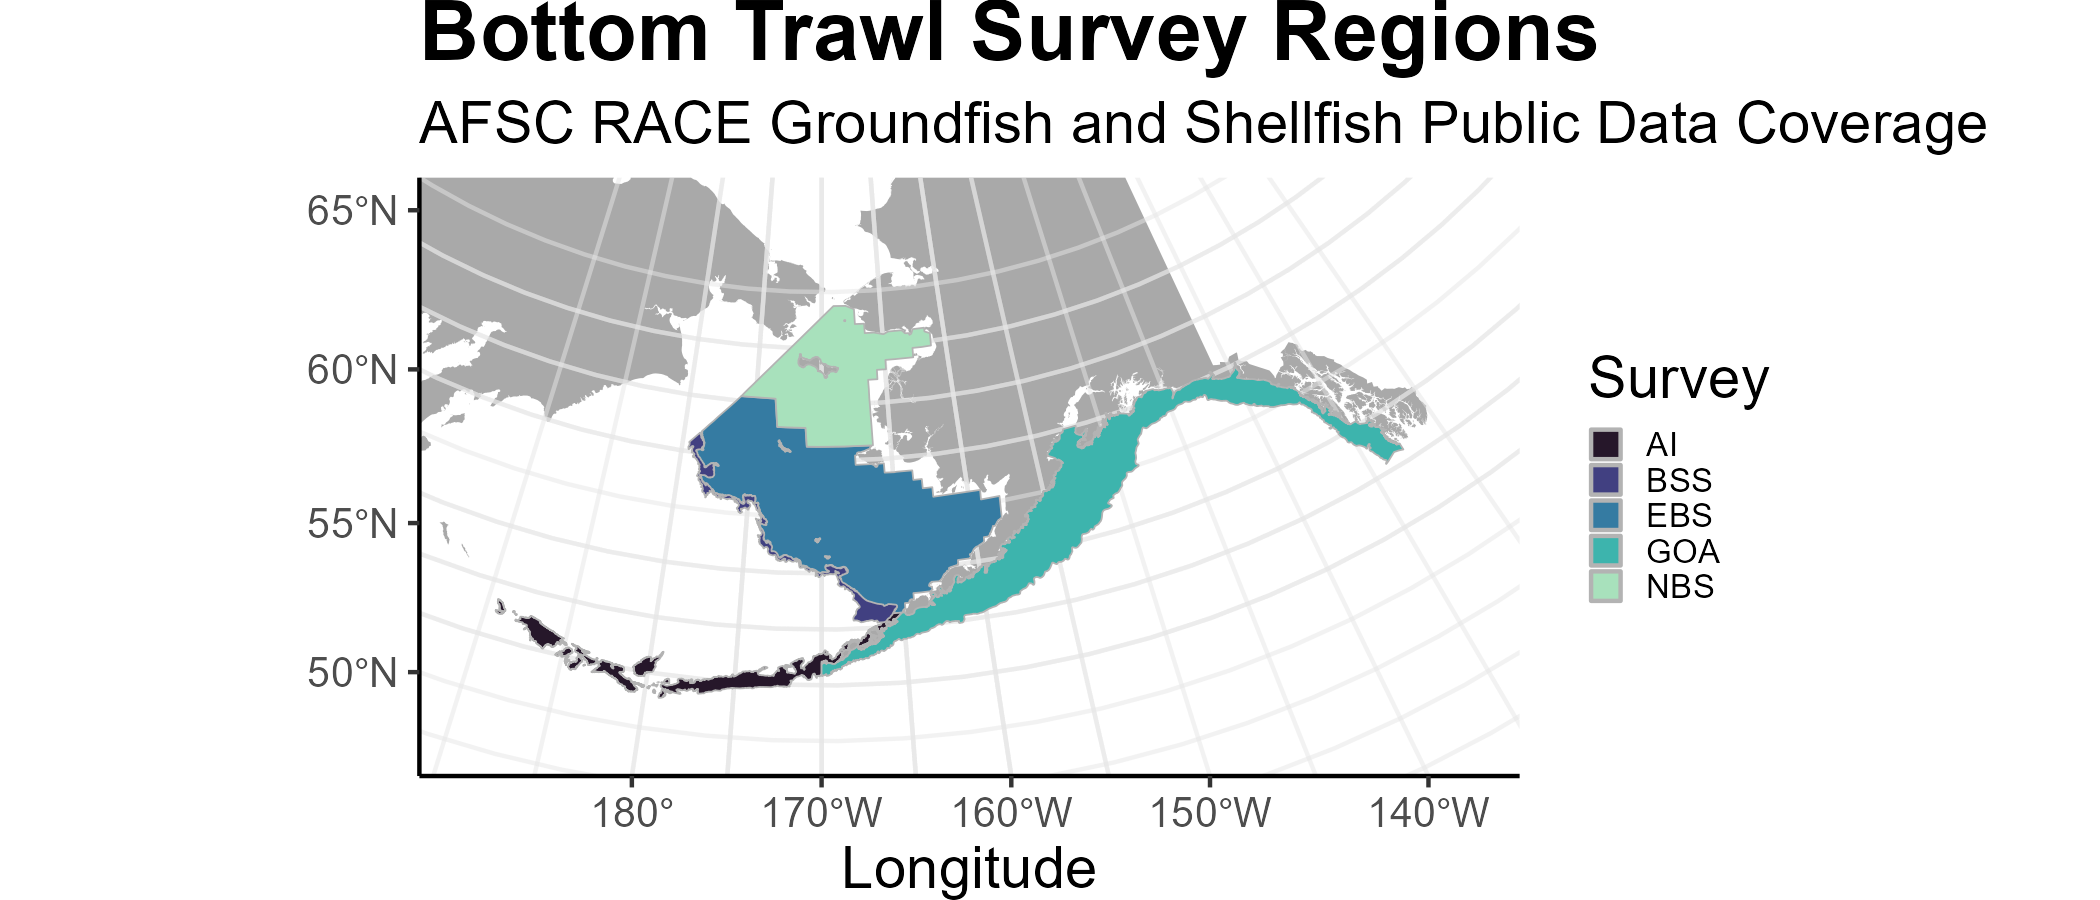
\includegraphics[width=7in,height=\textheight]{content/../img/survey_plot.png}

\begin{itemize}
\tightlist
\item
  \textbf{Aleutian Islands (AI)} (Von Szalay and Raring, 2020)

  \begin{itemize}
  \tightlist
  \item
    Triennial (1990s)/Biennial since 2000 in even years
  \item
    Modified Index-Stratified Random of Successful Stations Survey
    Design
  \end{itemize}
\item
  \textbf{Eastern Bering Sea Slope (BSS)} (Hoff, 2016)

  \begin{itemize}
  \tightlist
  \item
    Intermittent (funding dependent)
  \item
    Modified Index-Stratified Random of Successful Stations Survey
    Design
  \end{itemize}
\item
  \textbf{Eastern Bering Sea Shelf (EBS)} (Markowitz et al., 2023)

  \begin{itemize}
  \tightlist
  \item
    Annual
  \item
    Fixed stations at center of 20 x 20 nm grid
  \end{itemize}
\item
  \textbf{Gulf of Alaska (GOA)} (Von Szalay and Raring, 2018)

  \begin{itemize}
  \tightlist
  \item
    Triennial (1990s)/Biennial since 2001 in odd years
  \item
    Stratified Random Survey Design
  \end{itemize}
\item
  \textbf{Northern Bering Sea (NBS)} (Markowitz et al., 2023)

  \begin{itemize}
  \tightlist
  \item
    Biennial/Annual
  \item
    Fixed stations at center of 20 x 20 nm grid
  \end{itemize}
\end{itemize}

\global\setlength{\Oldarrayrulewidth}{\arrayrulewidth}

\global\setlength{\Oldtabcolsep}{\tabcolsep}

\setlength{\tabcolsep}{0pt}

\renewcommand*{\arraystretch}{1.5}



\providecommand{\ascline}[3]{\noalign{\global\arrayrulewidth #1}\arrayrulecolor[HTML]{#2}\cline{#3}}

\begin{longtable}[c]{|p{1.50in}|p{0.91in}|p{0.72in}|p{0.48in}|p{0.52in}|p{0.83in}|p{0.88in}}
\caption{Survey summary stats}\tabularnewline




\hhline{>{\arrayrulecolor[HTML]{000000}\global\arrayrulewidth=0pt}->{\arrayrulecolor[HTML]{000000}\global\arrayrulewidth=0pt}->{\arrayrulecolor[HTML]{000000}\global\arrayrulewidth=0pt}->{\arrayrulecolor[HTML]{000000}\global\arrayrulewidth=0pt}->{\arrayrulecolor[HTML]{000000}\global\arrayrulewidth=0pt}->{\arrayrulecolor[HTML]{000000}\global\arrayrulewidth=0pt}->{\arrayrulecolor[HTML]{000000}\global\arrayrulewidth=0pt}-}

\multicolumn{1}{>{\cellcolor[HTML]{CFCFCF}\raggedright}m{\dimexpr 1.5in+0\tabcolsep}}{\textcolor[HTML]{000000}{\fontsize{10}{10}\selectfont{\textbf{Survey}}}} & \multicolumn{1}{>{\cellcolor[HTML]{CFCFCF}\raggedleft}m{\dimexpr 0.91in+0\tabcolsep}}{\textcolor[HTML]{000000}{\fontsize{10}{10}\selectfont{\textbf{Survey\ Definition\ ID}}}} & \multicolumn{1}{>{\cellcolor[HTML]{CFCFCF}\raggedright}m{\dimexpr 0.72in+0\tabcolsep}}{\textcolor[HTML]{000000}{\fontsize{10}{10}\selectfont{\textbf{Years}}}} & \multicolumn{1}{>{\cellcolor[HTML]{CFCFCF}\raggedright}m{\dimexpr 0.48in+0\tabcolsep}}{\textcolor[HTML]{000000}{\fontsize{10}{10}\selectfont{\textbf{Depth\ (m)}}}} & \multicolumn{1}{>{\cellcolor[HTML]{CFCFCF}\raggedright}m{\dimexpr 0.52in+0\tabcolsep}}{\textcolor[HTML]{000000}{\fontsize{10}{10}\selectfont{\textbf{Area\ (km2)}}}} & \multicolumn{1}{>{\cellcolor[HTML]{CFCFCF}\raggedleft}m{\dimexpr 0.83in+0\tabcolsep}}{\textcolor[HTML]{000000}{\fontsize{10}{10}\selectfont{\textbf{\#\ Statistical\ Areas}}}} & \multicolumn{1}{>{\cellcolor[HTML]{CFCFCF}\raggedleft}m{\dimexpr 0.88in+0\tabcolsep}}{\textcolor[HTML]{000000}{\fontsize{10}{10}\selectfont{\textbf{\#\ Possible\ Stations}}}} \\

\noalign{\global\arrayrulewidth 0pt}\arrayrulecolor[HTML]{000000}

\endfirsthead 

\hhline{>{\arrayrulecolor[HTML]{000000}\global\arrayrulewidth=0pt}->{\arrayrulecolor[HTML]{000000}\global\arrayrulewidth=0pt}->{\arrayrulecolor[HTML]{000000}\global\arrayrulewidth=0pt}->{\arrayrulecolor[HTML]{000000}\global\arrayrulewidth=0pt}->{\arrayrulecolor[HTML]{000000}\global\arrayrulewidth=0pt}->{\arrayrulecolor[HTML]{000000}\global\arrayrulewidth=0pt}->{\arrayrulecolor[HTML]{000000}\global\arrayrulewidth=0pt}-}

\multicolumn{1}{>{\cellcolor[HTML]{CFCFCF}\raggedright}m{\dimexpr 1.5in+0\tabcolsep}}{\textcolor[HTML]{000000}{\fontsize{10}{10}\selectfont{\textbf{Survey}}}} & \multicolumn{1}{>{\cellcolor[HTML]{CFCFCF}\raggedleft}m{\dimexpr 0.91in+0\tabcolsep}}{\textcolor[HTML]{000000}{\fontsize{10}{10}\selectfont{\textbf{Survey\ Definition\ ID}}}} & \multicolumn{1}{>{\cellcolor[HTML]{CFCFCF}\raggedright}m{\dimexpr 0.72in+0\tabcolsep}}{\textcolor[HTML]{000000}{\fontsize{10}{10}\selectfont{\textbf{Years}}}} & \multicolumn{1}{>{\cellcolor[HTML]{CFCFCF}\raggedright}m{\dimexpr 0.48in+0\tabcolsep}}{\textcolor[HTML]{000000}{\fontsize{10}{10}\selectfont{\textbf{Depth\ (m)}}}} & \multicolumn{1}{>{\cellcolor[HTML]{CFCFCF}\raggedright}m{\dimexpr 0.52in+0\tabcolsep}}{\textcolor[HTML]{000000}{\fontsize{10}{10}\selectfont{\textbf{Area\ (km2)}}}} & \multicolumn{1}{>{\cellcolor[HTML]{CFCFCF}\raggedleft}m{\dimexpr 0.83in+0\tabcolsep}}{\textcolor[HTML]{000000}{\fontsize{10}{10}\selectfont{\textbf{\#\ Statistical\ Areas}}}} & \multicolumn{1}{>{\cellcolor[HTML]{CFCFCF}\raggedleft}m{\dimexpr 0.88in+0\tabcolsep}}{\textcolor[HTML]{000000}{\fontsize{10}{10}\selectfont{\textbf{\#\ Possible\ Stations}}}} \\

\noalign{\global\arrayrulewidth 0pt}\arrayrulecolor[HTML]{000000}

\endhead



\multicolumn{1}{>{\cellcolor[HTML]{EFEFEF}\raggedright}m{\dimexpr 1.5in+0\tabcolsep}}{\textcolor[HTML]{000000}{\fontsize{10}{10}\selectfont{Aleutian\ Islands\ Bottom\ Trawl\ Survey}}} & \multicolumn{1}{>{\cellcolor[HTML]{EFEFEF}\centering}m{\dimexpr 0.91in+0\tabcolsep}}{\textcolor[HTML]{000000}{\fontsize{10}{10}\selectfont{52}}} & \multicolumn{1}{>{\cellcolor[HTML]{EFEFEF}\raggedright}m{\dimexpr 0.72in+0\tabcolsep}}{\textcolor[HTML]{000000}{\fontsize{10}{10}\selectfont{2022\ -\ 1980\ (16)}}} & \multicolumn{1}{>{\cellcolor[HTML]{EFEFEF}\raggedright}m{\dimexpr 0.48in+0\tabcolsep}}{\textcolor[HTML]{000000}{\fontsize{10}{10}\selectfont{1\ -\ 500}}} & \multicolumn{1}{>{\cellcolor[HTML]{EFEFEF}\raggedright}m{\dimexpr 0.52in+0\tabcolsep}}{\textcolor[HTML]{000000}{\fontsize{10}{10}\selectfont{64,415.0}}} & \multicolumn{1}{>{\cellcolor[HTML]{EFEFEF}\raggedleft}m{\dimexpr 0.83in+0\tabcolsep}}{\textcolor[HTML]{000000}{\fontsize{10}{10}\selectfont{80}}} & \multicolumn{1}{>{\cellcolor[HTML]{EFEFEF}\raggedleft}m{\dimexpr 0.88in+0\tabcolsep}}{\textcolor[HTML]{000000}{\fontsize{10}{10}\selectfont{1,312}}} \\

\noalign{\global\arrayrulewidth 0pt}\arrayrulecolor[HTML]{000000}





\multicolumn{1}{>{\raggedright}m{\dimexpr 1.5in+0\tabcolsep}}{\textcolor[HTML]{000000}{\fontsize{10}{10}\selectfont{Eastern\ Bering\ Sea\ Slope\ Bottom\ Trawl\ Survey}}} & \multicolumn{1}{>{\centering}m{\dimexpr 0.91in+0\tabcolsep}}{\textcolor[HTML]{000000}{\fontsize{10}{10}\selectfont{78}}} & \multicolumn{1}{>{\raggedright}m{\dimexpr 0.72in+0\tabcolsep}}{\textcolor[HTML]{000000}{\fontsize{10}{10}\selectfont{2016\ -\ 2002\ (6)}}} & \multicolumn{1}{>{\raggedright}m{\dimexpr 0.48in+0\tabcolsep}}{\textcolor[HTML]{000000}{\fontsize{10}{10}\selectfont{201\ -\ 800}}} & \multicolumn{1}{>{\raggedright}m{\dimexpr 0.52in+0\tabcolsep}}{\textcolor[HTML]{000000}{\fontsize{10}{10}\selectfont{21,134.2}}} & \multicolumn{1}{>{\raggedleft}m{\dimexpr 0.83in+0\tabcolsep}}{\textcolor[HTML]{000000}{\fontsize{10}{10}\selectfont{4}}} & \multicolumn{1}{>{\raggedleft}m{\dimexpr 0.88in+0\tabcolsep}}{\textcolor[HTML]{000000}{\fontsize{10}{10}\selectfont{}}} \\

\noalign{\global\arrayrulewidth 0pt}\arrayrulecolor[HTML]{000000}





\multicolumn{1}{>{\cellcolor[HTML]{EFEFEF}\raggedright}m{\dimexpr 1.5in+0\tabcolsep}}{\textcolor[HTML]{000000}{\fontsize{10}{10}\selectfont{Eastern\ Bering\ Sea\ Crab/Groundfish\ Bottom\ Trawl\ Survey}}} & \multicolumn{1}{>{\cellcolor[HTML]{EFEFEF}\centering}m{\dimexpr 0.91in+0\tabcolsep}}{\textcolor[HTML]{000000}{\fontsize{10}{10}\selectfont{98}}} & \multicolumn{1}{>{\cellcolor[HTML]{EFEFEF}\raggedright}m{\dimexpr 0.72in+0\tabcolsep}}{\textcolor[HTML]{000000}{\fontsize{10}{10}\selectfont{2023\ -\ 1982\ (41)}}} & \multicolumn{1}{>{\cellcolor[HTML]{EFEFEF}\raggedright}m{\dimexpr 0.48in+0\tabcolsep}}{\textcolor[HTML]{000000}{\fontsize{10}{10}\selectfont{1\ -\ 200}}} & \multicolumn{1}{>{\cellcolor[HTML]{EFEFEF}\raggedright}m{\dimexpr 0.52in+0\tabcolsep}}{\textcolor[HTML]{000000}{\fontsize{10}{10}\selectfont{492,989.9}}} & \multicolumn{1}{>{\cellcolor[HTML]{EFEFEF}\raggedleft}m{\dimexpr 0.83in+0\tabcolsep}}{\textcolor[HTML]{000000}{\fontsize{10}{10}\selectfont{29}}} & \multicolumn{1}{>{\cellcolor[HTML]{EFEFEF}\raggedleft}m{\dimexpr 0.88in+0\tabcolsep}}{\textcolor[HTML]{000000}{\fontsize{10}{10}\selectfont{515}}} \\

\noalign{\global\arrayrulewidth 0pt}\arrayrulecolor[HTML]{000000}





\multicolumn{1}{>{\raggedright}m{\dimexpr 1.5in+0\tabcolsep}}{\textcolor[HTML]{000000}{\fontsize{10}{10}\selectfont{Gulf\ of\ Alaska\ Bottom\ Trawl\ Survey}}} & \multicolumn{1}{>{\centering}m{\dimexpr 0.91in+0\tabcolsep}}{\textcolor[HTML]{000000}{\fontsize{10}{10}\selectfont{47}}} & \multicolumn{1}{>{\raggedright}m{\dimexpr 0.72in+0\tabcolsep}}{\textcolor[HTML]{000000}{\fontsize{10}{10}\selectfont{2023\ -\ 1984\ (18)}}} & \multicolumn{1}{>{\raggedright}m{\dimexpr 0.48in+0\tabcolsep}}{\textcolor[HTML]{000000}{\fontsize{10}{10}\selectfont{1\ -\ 1,000}}} & \multicolumn{1}{>{\raggedright}m{\dimexpr 0.52in+0\tabcolsep}}{\textcolor[HTML]{000000}{\fontsize{10}{10}\selectfont{314,087.4}}} & \multicolumn{1}{>{\raggedleft}m{\dimexpr 0.83in+0\tabcolsep}}{\textcolor[HTML]{000000}{\fontsize{10}{10}\selectfont{39}}} & \multicolumn{1}{>{\raggedleft}m{\dimexpr 0.88in+0\tabcolsep}}{\textcolor[HTML]{000000}{\fontsize{10}{10}\selectfont{6,939}}} \\

\noalign{\global\arrayrulewidth 0pt}\arrayrulecolor[HTML]{000000}





\multicolumn{1}{>{\cellcolor[HTML]{EFEFEF}\raggedright}m{\dimexpr 1.5in+0\tabcolsep}}{\textcolor[HTML]{000000}{\fontsize{10}{10}\selectfont{Northern\ Bering\ Sea\ Crab/Groundfish\ Survey\ -\ Eastern\ Bering\ Sea\ Shelf\ Survey\ Extension}}} & \multicolumn{1}{>{\cellcolor[HTML]{EFEFEF}\centering}m{\dimexpr 0.91in+0\tabcolsep}}{\textcolor[HTML]{000000}{\fontsize{10}{10}\selectfont{143}}} & \multicolumn{1}{>{\cellcolor[HTML]{EFEFEF}\raggedright}m{\dimexpr 0.72in+0\tabcolsep}}{\textcolor[HTML]{000000}{\fontsize{10}{10}\selectfont{2022\ -\ 2010\ (5)}}} & \multicolumn{1}{>{\cellcolor[HTML]{EFEFEF}\raggedright}m{\dimexpr 0.48in+0\tabcolsep}}{\textcolor[HTML]{000000}{\fontsize{10}{10}\selectfont{1\ -\ 100}}} & \multicolumn{1}{>{\cellcolor[HTML]{EFEFEF}\raggedright}m{\dimexpr 0.52in+0\tabcolsep}}{\textcolor[HTML]{000000}{\fontsize{10}{10}\selectfont{198,866.8}}} & \multicolumn{1}{>{\cellcolor[HTML]{EFEFEF}\raggedleft}m{\dimexpr 0.83in+0\tabcolsep}}{\textcolor[HTML]{000000}{\fontsize{10}{10}\selectfont{4}}} & \multicolumn{1}{>{\cellcolor[HTML]{EFEFEF}\raggedleft}m{\dimexpr 0.88in+0\tabcolsep}}{\textcolor[HTML]{000000}{\fontsize{10}{10}\selectfont{144}}} \\

\noalign{\global\arrayrulewidth 0pt}\arrayrulecolor[HTML]{000000}





\end{longtable}



\arrayrulecolor[HTML]{000000}

\global\setlength{\arrayrulewidth}{\Oldarrayrulewidth}

\global\setlength{\tabcolsep}{\Oldtabcolsep}

\renewcommand*{\arraystretch}{1}

\hypertarget{survey-history}{%
\section{Survey History}\label{survey-history}}

\hypertarget{aleutian-islands-survey}{%
\subsection{Aleutian Islands Survey}\label{aleutian-islands-survey}}

\hypertarget{bering-sea-survey}{%
\subsection{Bering Sea Survey}\label{bering-sea-survey}}

\hypertarget{bering-sea-slope-survey}{%
\subsection{Bering Sea Slope Survey}\label{bering-sea-slope-survey}}

\hypertarget{gulf-of-alaska-survey}{%
\subsection{Gulf of Alaska Survey}\label{gulf-of-alaska-survey}}

\hypertarget{workflow}{%
\chapter{Workflow}\label{workflow}}

\textbf{Info incoming!}

\hypertarget{data-levels}{%
\section{Data levels}\label{data-levels}}

GAP produces numerous data products* that are subjected to different
levels of processing, ranging from raw to highly-derived. The
suitability of these data products for analysis varies and there is
ambiguity about which data products can be used for which purpose. This
ambiguity can create challenges in communicating about data products and
potentially lead to misunderstanding and misuse of data. One approach to
communicating about the level of processing applied to data products and
their suitability for analysis is to describe data products using a Data
Processing Level system. Data Processing Level systems are widely used
in earth system sciences to characterize the extent of processing that
has been applied to data products. For example, the NOAA National
Centers for Environmental Information (NCEI) Satellite Program uses a
Data Processing Level system to describe data on a scale of 0-4, where
Level 0 is raw data and Level 4 is model output or results from
analysis. Example of how
\href{https://ladsweb.modaps.eosdis.nasa.gov/search/}{NASA remote
sensing data products} are shared through a public data portal with
levels of data processing and documentation.

For more information, see
\href{https://docs.google.com/presentation/d/1rWSZpeghWJqzWMIa5oBc4BCoy-zy1Yue86RoTw58u6M/edit?usp=sharing}{Sean
Rohan's October 2022 SCRUGS presentation} on the topic.

\begin{itemize}
\tightlist
\item
  \textbf{Level 0}: Raw and unprocessed data. Ex: Data on the G drive,
  some tables in RACE\_DATA
\item
  \textbf{Level 1A}: Data products with QA/QC applied that may or may
  not be expanded to analysis units, but either not georeferenced or
  does not include full metadata. Ex: Some tables in RACE\_DATA and
  RACEBASE
\item
  \textbf{Level 2}: Analysis-ready data products that are derived for a
  standardized extent and account for zeros and missing/bad data. Ex:
  CPUE tables, some data products in public-facing archives and
  repositories
\item
  \textbf{Level 3}: Data products that are synthesized across a
  standardized extent, often inputs in a higher-level analytical
  product. Ex: Abundance indices, some data products in public-facing
  archives and repositories
\item
  \textbf{Level 4}: Analytically generated data products that are
  derived from lower-level data, often to inform management. Ex:
  Biological reference points from stock assessments, Essential Fish
  Habitat layers, indicators in Ecosystem Status Reports and Ecosystem
  and Socioeconomic Profiles
\end{itemize}

\hypertarget{news}{%
\chapter{News}\label{news}}

\hypertarget{early-2023}{%
\section{Early 2023}\label{early-2023}}

The main goal here to simplify the data management or to also
standardize the way stock assessors are using RACE data.

We have decided to undergo this organizational change to meet the
following best practices and long-term data goals. Let us know how we
can better meet these objectives and best work with IT:

\begin{itemize}
\tightlist
\item
  Minimize duplication (both in tables and in columns within tables)
\item
  Minimize schemata and Oracle objects to the extent possible
\item
  Streamlined integration of tables
\item
  Minimize work for data creators
\item
  Minimize confusion and obstacles for data users
\item
  Security and data management best practices
\end{itemize}

After the 2023 field season, we will deprecate the old AKFIN tables and
completely replace the current tables with new tables, outlined in this
document.

\part{GAP Production Data}

\hypertarget{data-description}{%
\section*{Data Description}\label{data-description}}
\addcontentsline{toc}{section}{Data Description}

\markright{Data Description}

The Resource Assessment and Conservation Engineering Division (RACE)
Groundfish Assessment Program (GAP) of the Alaska Fisheries Science
Center (AFSC) conducts fisheries-independent bottom trawl surveys to
monitor the condition of the demersal fish and crab stocks of Alaska.
These data are developed to describe the temporal distribution and
abundance of commercially and ecologically important groundfish species,
examine the changes in the species composition of the fauna over time
and space, and describe the physical environment of the groundfish
habitat.

Users must read and fully comprehend the metadata prior to use. Data
should not be used beyond the limits of the source scale.
Acknowledgement of NOAA, as the source from which these data were
obtained, in any publications and/or other representations of these
data, is suggested. These data are compiled and approved annually after
each summer survey season. The data from previous years are unlikely to
change substantially once published. Some survey data are excluded, such
as non-standard stations, surveys completed in earlier years using
different/non-standard gear, and special tows and non-standard data
collections.

\hypertarget{cite-this-data-1}{%
\section*{Cite this data}\label{cite-this-data-1}}
\addcontentsline{toc}{section}{Cite this data}

\markright{Cite this data}

Use the below
\href{https://github.com/afsc-gap-products/gap_products/blob/main/code/CITATION_GAPProducts.bib}{bibtext
citations}, as cited in our group's
\href{https://github.com/afsc-gap-products/citations/blob/main/cite/bibliography.bib}{citation
repository} for citing the data created and maintained in this repo
(NOAA Fisheries Alaska Fisheries Science Center, Goundfish Assessment
Program, 2023). Add ``note = \{Accessed: mm/dd/yyyy\}'' to append the
day this data was accessed.

\begin{verbatim}
@misc{GAPProducts,
  author = {{NOAA Fisheries Alaska Fisheries Science Center, Goundfish Assessment Program}},
  year = {2023}, 
  title = {AFSC Goundfish Assessment Program Design-Based Production Data},
  howpublished = {https://www.fisheries.noaa.gov/alaska/science-data/groundfish-assessment-program-bottom-trawl-surveys},
  publisher = {{U.S. Dep. Commer.}},
  copyright = {Public Domain} 
}
\end{verbatim}

\hypertarget{data-creation}{%
\section*{Data Creation}\label{data-creation}}
\addcontentsline{toc}{section}{Data Creation}

\markright{Data Creation}

These data are created using the
\href{https://github.com/afsc-gap-products/gapindex}{gapindex R
package}.

\hypertarget{data-description-1}{%
\chapter{Data description}\label{data-description-1}}

\hypertarget{data-created-in-this-repo}{%
\section{Data created in this repo}\label{data-created-in-this-repo}}

\hypertarget{agecomp}{%
\subsection{AGECOMP}\label{agecomp}}

Region-level age compositions by sex/length bin. This table was created
by the Resource Assessment and Conservation Engineering Division (RACE)
Groundfish Assessment Program (GAP) of the Alaska Fisheries Science
Center (AFSC). There are legal restrictions on access to the data. These
data are not intended for public dissemination and should not be shared
without the explicit written consent of the data managers and owners
(NOAA Fisheries). The GitHub repository for the scripts that created
this code can be found at
https://github.com/afsc-gap-products/gap\_products. For more information
about codes used in the tables, please refer to the survey code books
(https://www.fisheries.noaa.gov/resource/document/groundfish-survey-species-code-manual-and-data-codes-manual).
These data were last updated September 06, 2023.

Number of rows: 544301

Number of columns: 9

list(dataset = list(\texttt{Column\ name\ from\ data} = ``Column name
from data'', \texttt{Descriptive\ column\ Name} = ``Descriptive column
Name'', Units = ``Units'', \texttt{Oracle\ data\ type} = ``Oracle data
type'', \texttt{Column\ description} = ``Column description''), content
= list(content = list(data = list(list(txt = ``Column name from data'',
font.size = NA, italic = NA, bold = NA, underlined = NA, color = NA,
shading.color = NA, font.family = NA, hansi.family = NA, eastasia.family
= NA, cs.family = NA, vertical.align = NA, width = NA, height = NA, url
= NA, eq\_data = NA, word\_field\_data = NA, img\_data = list(NULL),
seq\_index = 1), list(txt = ``Descriptive column Name'', font.size = NA,
italic = NA, bold = NA, underlined = NA, color = NA, shading.color = NA,
font.family = NA, hansi.family = NA, eastasia.family = NA, cs.family =
NA, vertical.align = NA, width = NA, height = NA, url = NA, eq\_data =
NA, word\_field\_data = NA, img\_data = list(NULL), seq\_index = 1),
list(txt = ``Units'', font.size = NA, italic = NA, bold = NA, underlined
= NA, color = NA, shading.color = NA, font.family = NA, hansi.family =
NA, eastasia.family = NA, cs.family = NA, vertical.align = NA, width =
NA, height = NA, url = NA, eq\_data = NA, word\_field\_data = NA,
img\_data = list(NULL), seq\_index = 1), list(txt = ``Oracle data
type'', font.size = NA, italic = NA, bold = NA, underlined = NA, color =
NA, shading.color = NA, font.family = NA, hansi.family = NA,
eastasia.family = NA, cs.family = NA, vertical.align = NA, width = NA,
height = NA, url = NA, eq\_data = NA, word\_field\_data = NA, img\_data
= list(NULL), seq\_index = 1), list(txt = ``Column description'',
font.size = NA, italic = NA, bold = NA, underlined = NA, color = NA,
shading.color = NA, font.family = NA, hansi.family = NA, eastasia.family
= NA, cs.family = NA, vertical.align = NA, width = NA, height = NA, url
= NA, eq\_data = NA, word\_field\_data = NA, img\_data = list(NULL),
seq\_index = 1)), keys = c(``Column name from data'', ``Descriptive
column Name'', ``Units'', ``Oracle data type'', ``Column description''
), nrow = 1, ncol = 5, default = list(list(txt = ````, font.size = NA,
italic = NA, bold = NA, underlined = NA, color = NA, shading.color = NA,
font.family = NA, hansi.family = NA, eastasia.family = NA, cs.family =
NA, vertical.align = NA, width = NA, height = NA, url = NA, eq\_data =
NA, word\_field\_data = NA, img\_data = list(NULL), seq\_index = 1)))),
col\_keys = c(''Column name from data'', ``Descriptive column Name'',
``Units'', ``Oracle data type'', ``Column description''), colwidths =
c(0.75, 0.75, 0.75, 0.75, 0.75), rowheights = 0.25, hrule = ``auto'',
spans = list(rows = c(1, 1, 1, 1, 1), columns = c(1, 1, 1, 1, 1)),
styles = list(cells = list(vertical.align = list(data = c(``center'',
``center'', ``center'', ``center'', ``center''), keys = c(``Column name
from data'', ``Descriptive column Name'', ``Units'', ``Oracle data
type'', ``Column description''), nrow = 1, ncol = 5, default =
``center''), width = list(data = c(NA, NA, NA, NA, NA), keys =
c(``Column name from data'', ``Descriptive column Name'', ``Units'',
``Oracle data type'', ``Column description''), nrow = 1, ncol = 5,
default = NA), height = list(data = c(NA, NA, NA, NA, NA), keys =
c(``Column name from data'', ``Descriptive column Name'', ``Units'',
``Oracle data type'', ``Column description''), nrow = 1, ncol = 5,
default = NA), margin.bottom = list(data = c(0, 0, 0, 0, 0), keys =
c(``Column name from data'', ``Descriptive column Name'', ``Units'',
``Oracle data type'', ``Column description''), nrow = 1, ncol = 5,
default = 0), margin.top = list(data = c(0, 0, 0, 0, 0), keys =
c(``Column name from data'', ``Descriptive column Name'', ``Units'',
``Oracle data type'', ``Column description''), nrow = 1, ncol = 5,
default = 0), margin.left = list(data = c(0, 0, 0, 0, 0), keys =
c(``Column name from data'', ``Descriptive column Name'', ``Units'',
``Oracle data type'', ``Column description''), nrow = 1, ncol = 5,
default = 0), margin.right = list(data = c(0, 0, 0, 0, 0), keys =
c(``Column name from data'', ``Descriptive column Name'', ``Units'',
``Oracle data type'', ``Column description''), nrow = 1, ncol = 5,
default = 0), border.width.bottom = list( data = c(0, 0, 0, 0, 0), keys
= c(``Column name from data'', ``Descriptive column Name'', ``Units'',
``Oracle data type'', ``Column description''), nrow = 1, ncol = 5,
default = 0), border.width.top = list(data = c(0, 0, 0, 0, 0), keys =
c(``Column name from data'', ``Descriptive column Name'', ``Units'',
``Oracle data type'', ``Column description''), nrow = 1, ncol = 5,
default = 0), border.width.left = list(data = c(0, 0, 0, 0, 0), keys =
c(``Column name from data'', ``Descriptive column Name'', ``Units'',
``Oracle data type'', ``Column description''), nrow = 1, ncol = 5,
default = 0), border.width.right = list(data = c(0, 0, 0, 0, 0), keys =
c(``Column name from data'', ``Descriptive column Name'', ``Units'',
``Oracle data type'', ``Column description''), nrow = 1, ncol = 5,
default = 0), border.color.bottom = list(data = c(``black'', ``black'',
``black'', ``black'', ``black''), keys = c(``Column name from data'',
``Descriptive column Name'', ``Units'', ``Oracle data type'', ``Column
description''), nrow = 1, ncol = 5, default = ``transparent''),
border.color.top = list( data = c(``black'', ``black'', ``black'',
``black'', ``black''), keys = c(``Column name from data'', ``Descriptive
column Name'', ``Units'', ``Oracle data type'', ``Column description''),
nrow = 1, ncol = 5, default = ``transparent''), border.color.left =
list(data = c(``black'', ``black'', ``black'', ``black'', ``black''),
keys = c(``Column name from data'', ``Descriptive column Name'',
``Units'', ``Oracle data type'', ``Column description''), nrow = 1, ncol
= 5, default = ``transparent''), border.color.right = list(data =
c(``black'', ``black'', ``black'', ``black'', ``black''), keys =
c(``Column name from data'', ``Descriptive column Name'', ``Units'',
``Oracle data type'', ``Column description''), nrow = 1, ncol = 5,
default = ``transparent''), border.style.bottom = list(data =
c(``solid'', ``solid'', ``solid'', ``solid'', ``solid''), keys =
c(``Column name from data'', ``Descriptive column Name'', ``Units'',
``Oracle data type'', ``Column description''), nrow = 1, ncol = 5,
default = ``solid''), border.style.top = list(data = c(``solid'',
``solid'', ``solid'', ``solid'', ``solid'' ), keys = c(``Column name
from data'', ``Descriptive column Name'', ``Units'', ``Oracle data
type'', ``Column description''), nrow = 1, ncol = 5, default =
``solid''), border.style.left = list(data = c(``solid'', ``solid'',
``solid'', ``solid'', ``solid''), keys = c(``Column name from data'',
``Descriptive column Name'', ``Units'', ``Oracle data type'', ``Column
description''), nrow = 1, ncol = 5, default = ``solid''),
border.style.right = list(data = c(``solid'', ``solid'', ``solid'',
``solid'', ``solid''), keys = c(``Column name from data'', ``Descriptive
column Name'', ``Units'', ``Oracle data type'', ``Column description''),
nrow = 1, ncol = 5, default = ``solid''), text.direction = list(data =
c(``lrtb'', ``lrtb'', ``lrtb'', ``lrtb'', ``lrtb''), keys = c(``Column
name from data'', ``Descriptive column Name'', ``Units'', ``Oracle data
type'', ``Column description''), nrow = 1, ncol = 5, default =
``lrtb''), background.color = list(data = c(``\#CFCFCF'', ``\#CFCFCF'',
``\#CFCFCF'', ``\#CFCFCF'', ``\#CFCFCF''), keys = c(``Column name from
data'', ``Descriptive column Name'', ``Units'', ``Oracle data type'',
``Column description''), nrow = 1, ncol = 5, default = ``transparent''),
hrule = list(data = c(``auto'', ``auto'', ``auto'', ``auto'', ``auto''),
keys = c(``Column name from data'', ``Descriptive column Name'',
``Units'', ``Oracle data type'', ``Column description''), nrow = 1, ncol
= 5, default = ``auto'')), pars = list(text.align = list(data =
c(``left'', ``left'', ``left'', ``left'', ``left''), keys = c(``Column
name from data'', ``Descriptive column Name'', ``Units'', ``Oracle data
type'', ``Column description''), nrow = 1, ncol = 5, default =
``left''), padding.bottom = list(data = c(5, 5, 5, 5, 5), keys =
c(``Column name from data'', ``Descriptive column Name'', ``Units'',
``Oracle data type'', ``Column description''), nrow = 1, ncol = 5,
default = 5), padding.top = list(data = c(5, 5, 5, 5, 5), keys =
c(``Column name from data'', ``Descriptive column Name'', ``Units'',
``Oracle data type'', ``Column description''), nrow = 1, ncol = 5,
default = 5), padding.left = list(data = c(5, 5, 5, 5, 5), keys =
c(``Column name from data'', ``Descriptive column Name'', ``Units'',
``Oracle data type'', ``Column description''), nrow = 1, ncol = 5,
default = 5), padding.right = list(data = c(5, 5, 5, 5, 5), keys =
c(``Column name from data'', ``Descriptive column Name'', ``Units'',
``Oracle data type'', ``Column description''), nrow = 1, ncol = 5,
default = 5), line\_spacing = list(data = c(1, 1, 1, 1, 1), keys =
c(``Column name from data'', ``Descriptive column Name'', ``Units'',
``Oracle data type'', ``Column description''), nrow = 1, ncol = 5,
default = 1), border.width.bottom = list(data = c(0, 0, 0, 0, 0), keys =
c(``Column name from data'', ``Descriptive column Name'', ``Units'',
``Oracle data type'', ``Column description''), nrow = 1, ncol = 5,
default = 0), border.width.top = list(data = c(0, 0, 0, 0, 0), keys =
c(``Column name from data'', ``Descriptive column Name'', ``Units'',
``Oracle data type'', ``Column description''), nrow = 1, ncol = 5,
default = 0), border.width.left = list(data = c(0, 0, 0, 0, 0), keys =
c(``Column name from data'', ``Descriptive column Name'', ``Units'',
``Oracle data type'', ``Column description'' ), nrow = 1, ncol = 5,
default = 0), border.width.right = list(data = c(0, 0, 0, 0, 0), keys =
c(``Column name from data'', ``Descriptive column Name'', ``Units'',
``Oracle data type'', ``Column description''), nrow = 1, ncol = 5,
default = 0), border.color.bottom = list(data = c(``black'', ``black'',
``black'', ``black'', ``black''), keys = c(``Column name from data'',
``Descriptive column Name'', ``Units'', ``Oracle data type'', ``Column
description''), nrow = 1, ncol = 5, default = ``black''),
border.color.top = list(data = c(``black'', ``black'', ``black'',
``black'', ``black''), keys = c(``Column name from data'', ``Descriptive
column Name'', ``Units'', ``Oracle data type'', ``Column description''),
nrow = 1, ncol = 5, default = ``black''), border.color.left = list(data
= c(``black'', ``black'', ``black'', ``black'', ``black''), keys =
c(``Column name from data'', ``Descriptive column Name'', ``Units'',
``Oracle data type'', ``Column description''), nrow = 1, ncol = 5,
default = ``black''), border.color.right = list(data = c(``black'',
``black'', ``black'', ``black'', ``black'' ), keys = c(``Column name
from data'', ``Descriptive column Name'', ``Units'', ``Oracle data
type'', ``Column description''), nrow = 1, ncol = 5, default =
``black''), border.style.bottom = list(data = c(``solid'', ``solid'',
``solid'', ``solid'', ``solid''), keys = c(``Column name from data'',
``Descriptive column Name'', ``Units'', ``Oracle data type'', ``Column
description''), nrow = 1, ncol = 5, default = ``solid''),
border.style.top = list(data = c(``solid'', ``solid'', ``solid'',
``solid'', ``solid''), keys = c(``Column name from data'', ``Descriptive
column Name'', ``Units'', ``Oracle data type'', ``Column description''),
nrow = 1, ncol = 5, default = ``solid''), border.style.left = list(data
= c(``solid'', ``solid'', ``solid'', ``solid'', ``solid''), keys =
c(``Column name from data'', ``Descriptive column Name'', ``Units'',
``Oracle data type'', ``Column description''), nrow = 1, ncol = 5,
default = ``solid''), border.style.right = list(data = c(``solid'',
``solid'', ``solid'', ``solid'', ``solid''), keys = c(``Column name from
data'', ``Descriptive column Name'', ``Units'', ``Oracle data type'',
``Column description''), nrow = 1, ncol = 5, default = ``solid''),
shading.color = list(data = c(``transparent'', ``transparent'',
``transparent'', ``transparent'', ``transparent''), keys = c(``Column
name from data'', ``Descriptive column Name'', ``Units'', ``Oracle data
type'', ``Column description''), nrow = 1, ncol = 5, default =
``transparent''), keep\_with\_next = list(data = c(FALSE, FALSE, FALSE,
FALSE, FALSE), keys = c(``Column name from data'', ``Descriptive column
Name'', ``Units'', ``Oracle data type'', ``Column description''), nrow =
1, ncol = 5, default = FALSE)), text = list(color = list(data =
c(``black'', ``black'', ``black'', ``black'', ``black''), keys =
c(``Column name from data'', ``Descriptive column Name'', ``Units'',
``Oracle data type'', ``Column description''), nrow = 1, ncol = 5,
default = ``black''), font.size = list(data = c(11, 11, 11, 11, 11),
keys = c(``Column name from data'', ``Descriptive column Name'',
``Units'', ``Oracle data type'', ``Column description''), nrow = 1, ncol
= 5, default = 11), bold = list( data = c(TRUE, TRUE, TRUE, TRUE, TRUE),
keys = c(``Column name from data'', ``Descriptive column Name'',
``Units'', ``Oracle data type'', ``Column description''), nrow = 1, ncol
= 5, default = FALSE), italic = list(data = c(FALSE, FALSE, FALSE,
FALSE, FALSE), keys = c(``Column name from data'', ``Descriptive column
Name'', ``Units'', ``Oracle data type'', ``Column description''), nrow =
1, ncol = 5, default = FALSE), underlined = list(data = c(FALSE, FALSE,
FALSE, FALSE, FALSE), keys = c(``Column name from data'', ``Descriptive
column Name'', ``Units'', ``Oracle data type'', ``Column description''),
nrow = 1, ncol = 5, default = FALSE), font.family = list(data =
c(``Arial'', ``Arial'', ``Arial'', ``Arial'', ``Arial''), keys =
c(``Column name from data'', ``Descriptive column Name'', ``Units'',
``Oracle data type'', ``Column description''), nrow = 1, ncol = 5,
default = ``Arial''), hansi.family = list(data = c(``Arial'', ``Arial'',
``Arial'', ``Arial'', ``Arial''), keys = c(``Column name from data'',
``Descriptive column Name'', ``Units'', ``Oracle data type'', ``Column
description''), nrow = 1, ncol = 5, default = ``Arial''),
eastasia.family = list(data = c(``Arial'', ``Arial'', ``Arial'',
``Arial'', ``Arial''), keys = c(``Column name from data'', ``Descriptive
column Name'', ``Units'', ``Oracle data type'', ``Column description''),
nrow = 1, ncol = 5, default = ``Arial''), cs.family = list(data =
c(``Arial'', ``Arial'', ``Arial'', ``Arial'', ``Arial''), keys =
c(``Column name from data'', ``Descriptive column Name'', ``Units'',
``Oracle data type'', ``Column description''), nrow = 1, ncol = 5,
default = ``Arial''), vertical.align = list(data = c(``baseline'',
``baseline'', ``baseline'', ``baseline'', ``baseline''), keys =
c(``Column name from data'', ``Descriptive column Name'', ``Units'',
``Oracle data type'', ``Column description''), nrow = 1, ncol = 5,
default = ``baseline''), shading.color = list(data = c(``transparent'',
``transparent'', ``transparent'', ``transparent'', ``transparent''),
keys = c(``Column name from data'', ``Descriptive column Name'',
``Units'', ``Oracle data type'', ``Column description''), nrow = 1, ncol
= 5, default = ``transparent''))))

\hypertarget{area}{%
\subsection{AREA}\label{area}}

This reference table stores all metadata and estimates for all estimates
of stratum and subarea area estimates. Use this table with the
STRATUM\_GROUPS and SURVEY\_DESIGN tables. by the Resource Assessment
and Conservation Engineering Division (RACE) Groundfish Assessment
Program (GAP) of the Alaska Fisheries Science Center (AFSC). There are
legal restrictions on access to the data. These data are not intended
for public dissemination and should not be shared without the explicit
written consent of the data managers and owners (NOAA Fisheries). The
GitHub repository for the scripts that created this code can be found at
https://github.com/afsc-gap-products/gap\_products. For more information
about codes used in the tables, please refer to the survey code books
(https://www.fisheries.noaa.gov/resource/document/groundfish-survey-species-code-manual-and-data-codes-manual).
These data were last updated June 27, 2023.

Number of rows: 443

Number of columns: 10

list(dataset = list(\texttt{Column\ name\ from\ data} = ``Column name
from data'', \texttt{Descriptive\ column\ Name} = ``Descriptive column
Name'', Units = ``Units'', \texttt{Oracle\ data\ type} = ``Oracle data
type'', \texttt{Column\ description} = ``Column description''), content
= list(content = list(data = list(list(txt = ``Column name from data'',
font.size = NA, italic = NA, bold = NA, underlined = NA, color = NA,
shading.color = NA, font.family = NA, hansi.family = NA, eastasia.family
= NA, cs.family = NA, vertical.align = NA, width = NA, height = NA, url
= NA, eq\_data = NA, word\_field\_data = NA, img\_data = list(NULL),
seq\_index = 1), list(txt = ``Descriptive column Name'', font.size = NA,
italic = NA, bold = NA, underlined = NA, color = NA, shading.color = NA,
font.family = NA, hansi.family = NA, eastasia.family = NA, cs.family =
NA, vertical.align = NA, width = NA, height = NA, url = NA, eq\_data =
NA, word\_field\_data = NA, img\_data = list(NULL), seq\_index = 1),
list(txt = ``Units'', font.size = NA, italic = NA, bold = NA, underlined
= NA, color = NA, shading.color = NA, font.family = NA, hansi.family =
NA, eastasia.family = NA, cs.family = NA, vertical.align = NA, width =
NA, height = NA, url = NA, eq\_data = NA, word\_field\_data = NA,
img\_data = list(NULL), seq\_index = 1), list(txt = ``Oracle data
type'', font.size = NA, italic = NA, bold = NA, underlined = NA, color =
NA, shading.color = NA, font.family = NA, hansi.family = NA,
eastasia.family = NA, cs.family = NA, vertical.align = NA, width = NA,
height = NA, url = NA, eq\_data = NA, word\_field\_data = NA, img\_data
= list(NULL), seq\_index = 1), list(txt = ``Column description'',
font.size = NA, italic = NA, bold = NA, underlined = NA, color = NA,
shading.color = NA, font.family = NA, hansi.family = NA, eastasia.family
= NA, cs.family = NA, vertical.align = NA, width = NA, height = NA, url
= NA, eq\_data = NA, word\_field\_data = NA, img\_data = list(NULL),
seq\_index = 1)), keys = c(``Column name from data'', ``Descriptive
column Name'', ``Units'', ``Oracle data type'', ``Column description''
), nrow = 1, ncol = 5, default = list(list(txt = ````, font.size = NA,
italic = NA, bold = NA, underlined = NA, color = NA, shading.color = NA,
font.family = NA, hansi.family = NA, eastasia.family = NA, cs.family =
NA, vertical.align = NA, width = NA, height = NA, url = NA, eq\_data =
NA, word\_field\_data = NA, img\_data = list(NULL), seq\_index = 1)))),
col\_keys = c(''Column name from data'', ``Descriptive column Name'',
``Units'', ``Oracle data type'', ``Column description''), colwidths =
c(0.75, 0.75, 0.75, 0.75, 0.75), rowheights = 0.25, hrule = ``auto'',
spans = list(rows = c(1, 1, 1, 1, 1), columns = c(1, 1, 1, 1, 1)),
styles = list(cells = list(vertical.align = list(data = c(``center'',
``center'', ``center'', ``center'', ``center''), keys = c(``Column name
from data'', ``Descriptive column Name'', ``Units'', ``Oracle data
type'', ``Column description''), nrow = 1, ncol = 5, default =
``center''), width = list(data = c(NA, NA, NA, NA, NA), keys =
c(``Column name from data'', ``Descriptive column Name'', ``Units'',
``Oracle data type'', ``Column description''), nrow = 1, ncol = 5,
default = NA), height = list(data = c(NA, NA, NA, NA, NA), keys =
c(``Column name from data'', ``Descriptive column Name'', ``Units'',
``Oracle data type'', ``Column description''), nrow = 1, ncol = 5,
default = NA), margin.bottom = list(data = c(0, 0, 0, 0, 0), keys =
c(``Column name from data'', ``Descriptive column Name'', ``Units'',
``Oracle data type'', ``Column description''), nrow = 1, ncol = 5,
default = 0), margin.top = list(data = c(0, 0, 0, 0, 0), keys =
c(``Column name from data'', ``Descriptive column Name'', ``Units'',
``Oracle data type'', ``Column description''), nrow = 1, ncol = 5,
default = 0), margin.left = list(data = c(0, 0, 0, 0, 0), keys =
c(``Column name from data'', ``Descriptive column Name'', ``Units'',
``Oracle data type'', ``Column description''), nrow = 1, ncol = 5,
default = 0), margin.right = list(data = c(0, 0, 0, 0, 0), keys =
c(``Column name from data'', ``Descriptive column Name'', ``Units'',
``Oracle data type'', ``Column description''), nrow = 1, ncol = 5,
default = 0), border.width.bottom = list( data = c(0, 0, 0, 0, 0), keys
= c(``Column name from data'', ``Descriptive column Name'', ``Units'',
``Oracle data type'', ``Column description''), nrow = 1, ncol = 5,
default = 0), border.width.top = list(data = c(0, 0, 0, 0, 0), keys =
c(``Column name from data'', ``Descriptive column Name'', ``Units'',
``Oracle data type'', ``Column description''), nrow = 1, ncol = 5,
default = 0), border.width.left = list(data = c(0, 0, 0, 0, 0), keys =
c(``Column name from data'', ``Descriptive column Name'', ``Units'',
``Oracle data type'', ``Column description''), nrow = 1, ncol = 5,
default = 0), border.width.right = list(data = c(0, 0, 0, 0, 0), keys =
c(``Column name from data'', ``Descriptive column Name'', ``Units'',
``Oracle data type'', ``Column description''), nrow = 1, ncol = 5,
default = 0), border.color.bottom = list(data = c(``black'', ``black'',
``black'', ``black'', ``black''), keys = c(``Column name from data'',
``Descriptive column Name'', ``Units'', ``Oracle data type'', ``Column
description''), nrow = 1, ncol = 5, default = ``transparent''),
border.color.top = list( data = c(``black'', ``black'', ``black'',
``black'', ``black''), keys = c(``Column name from data'', ``Descriptive
column Name'', ``Units'', ``Oracle data type'', ``Column description''),
nrow = 1, ncol = 5, default = ``transparent''), border.color.left =
list(data = c(``black'', ``black'', ``black'', ``black'', ``black''),
keys = c(``Column name from data'', ``Descriptive column Name'',
``Units'', ``Oracle data type'', ``Column description''), nrow = 1, ncol
= 5, default = ``transparent''), border.color.right = list(data =
c(``black'', ``black'', ``black'', ``black'', ``black''), keys =
c(``Column name from data'', ``Descriptive column Name'', ``Units'',
``Oracle data type'', ``Column description''), nrow = 1, ncol = 5,
default = ``transparent''), border.style.bottom = list(data =
c(``solid'', ``solid'', ``solid'', ``solid'', ``solid''), keys =
c(``Column name from data'', ``Descriptive column Name'', ``Units'',
``Oracle data type'', ``Column description''), nrow = 1, ncol = 5,
default = ``solid''), border.style.top = list(data = c(``solid'',
``solid'', ``solid'', ``solid'', ``solid'' ), keys = c(``Column name
from data'', ``Descriptive column Name'', ``Units'', ``Oracle data
type'', ``Column description''), nrow = 1, ncol = 5, default =
``solid''), border.style.left = list(data = c(``solid'', ``solid'',
``solid'', ``solid'', ``solid''), keys = c(``Column name from data'',
``Descriptive column Name'', ``Units'', ``Oracle data type'', ``Column
description''), nrow = 1, ncol = 5, default = ``solid''),
border.style.right = list(data = c(``solid'', ``solid'', ``solid'',
``solid'', ``solid''), keys = c(``Column name from data'', ``Descriptive
column Name'', ``Units'', ``Oracle data type'', ``Column description''),
nrow = 1, ncol = 5, default = ``solid''), text.direction = list(data =
c(``lrtb'', ``lrtb'', ``lrtb'', ``lrtb'', ``lrtb''), keys = c(``Column
name from data'', ``Descriptive column Name'', ``Units'', ``Oracle data
type'', ``Column description''), nrow = 1, ncol = 5, default =
``lrtb''), background.color = list(data = c(``\#CFCFCF'', ``\#CFCFCF'',
``\#CFCFCF'', ``\#CFCFCF'', ``\#CFCFCF''), keys = c(``Column name from
data'', ``Descriptive column Name'', ``Units'', ``Oracle data type'',
``Column description''), nrow = 1, ncol = 5, default = ``transparent''),
hrule = list(data = c(``auto'', ``auto'', ``auto'', ``auto'', ``auto''),
keys = c(``Column name from data'', ``Descriptive column Name'',
``Units'', ``Oracle data type'', ``Column description''), nrow = 1, ncol
= 5, default = ``auto'')), pars = list(text.align = list(data =
c(``left'', ``left'', ``left'', ``left'', ``left''), keys = c(``Column
name from data'', ``Descriptive column Name'', ``Units'', ``Oracle data
type'', ``Column description''), nrow = 1, ncol = 5, default =
``left''), padding.bottom = list(data = c(5, 5, 5, 5, 5), keys =
c(``Column name from data'', ``Descriptive column Name'', ``Units'',
``Oracle data type'', ``Column description''), nrow = 1, ncol = 5,
default = 5), padding.top = list(data = c(5, 5, 5, 5, 5), keys =
c(``Column name from data'', ``Descriptive column Name'', ``Units'',
``Oracle data type'', ``Column description''), nrow = 1, ncol = 5,
default = 5), padding.left = list(data = c(5, 5, 5, 5, 5), keys =
c(``Column name from data'', ``Descriptive column Name'', ``Units'',
``Oracle data type'', ``Column description''), nrow = 1, ncol = 5,
default = 5), padding.right = list(data = c(5, 5, 5, 5, 5), keys =
c(``Column name from data'', ``Descriptive column Name'', ``Units'',
``Oracle data type'', ``Column description''), nrow = 1, ncol = 5,
default = 5), line\_spacing = list(data = c(1, 1, 1, 1, 1), keys =
c(``Column name from data'', ``Descriptive column Name'', ``Units'',
``Oracle data type'', ``Column description''), nrow = 1, ncol = 5,
default = 1), border.width.bottom = list(data = c(0, 0, 0, 0, 0), keys =
c(``Column name from data'', ``Descriptive column Name'', ``Units'',
``Oracle data type'', ``Column description''), nrow = 1, ncol = 5,
default = 0), border.width.top = list(data = c(0, 0, 0, 0, 0), keys =
c(``Column name from data'', ``Descriptive column Name'', ``Units'',
``Oracle data type'', ``Column description''), nrow = 1, ncol = 5,
default = 0), border.width.left = list(data = c(0, 0, 0, 0, 0), keys =
c(``Column name from data'', ``Descriptive column Name'', ``Units'',
``Oracle data type'', ``Column description'' ), nrow = 1, ncol = 5,
default = 0), border.width.right = list(data = c(0, 0, 0, 0, 0), keys =
c(``Column name from data'', ``Descriptive column Name'', ``Units'',
``Oracle data type'', ``Column description''), nrow = 1, ncol = 5,
default = 0), border.color.bottom = list(data = c(``black'', ``black'',
``black'', ``black'', ``black''), keys = c(``Column name from data'',
``Descriptive column Name'', ``Units'', ``Oracle data type'', ``Column
description''), nrow = 1, ncol = 5, default = ``black''),
border.color.top = list(data = c(``black'', ``black'', ``black'',
``black'', ``black''), keys = c(``Column name from data'', ``Descriptive
column Name'', ``Units'', ``Oracle data type'', ``Column description''),
nrow = 1, ncol = 5, default = ``black''), border.color.left = list(data
= c(``black'', ``black'', ``black'', ``black'', ``black''), keys =
c(``Column name from data'', ``Descriptive column Name'', ``Units'',
``Oracle data type'', ``Column description''), nrow = 1, ncol = 5,
default = ``black''), border.color.right = list(data = c(``black'',
``black'', ``black'', ``black'', ``black'' ), keys = c(``Column name
from data'', ``Descriptive column Name'', ``Units'', ``Oracle data
type'', ``Column description''), nrow = 1, ncol = 5, default =
``black''), border.style.bottom = list(data = c(``solid'', ``solid'',
``solid'', ``solid'', ``solid''), keys = c(``Column name from data'',
``Descriptive column Name'', ``Units'', ``Oracle data type'', ``Column
description''), nrow = 1, ncol = 5, default = ``solid''),
border.style.top = list(data = c(``solid'', ``solid'', ``solid'',
``solid'', ``solid''), keys = c(``Column name from data'', ``Descriptive
column Name'', ``Units'', ``Oracle data type'', ``Column description''),
nrow = 1, ncol = 5, default = ``solid''), border.style.left = list(data
= c(``solid'', ``solid'', ``solid'', ``solid'', ``solid''), keys =
c(``Column name from data'', ``Descriptive column Name'', ``Units'',
``Oracle data type'', ``Column description''), nrow = 1, ncol = 5,
default = ``solid''), border.style.right = list(data = c(``solid'',
``solid'', ``solid'', ``solid'', ``solid''), keys = c(``Column name from
data'', ``Descriptive column Name'', ``Units'', ``Oracle data type'',
``Column description''), nrow = 1, ncol = 5, default = ``solid''),
shading.color = list(data = c(``transparent'', ``transparent'',
``transparent'', ``transparent'', ``transparent''), keys = c(``Column
name from data'', ``Descriptive column Name'', ``Units'', ``Oracle data
type'', ``Column description''), nrow = 1, ncol = 5, default =
``transparent''), keep\_with\_next = list(data = c(FALSE, FALSE, FALSE,
FALSE, FALSE), keys = c(``Column name from data'', ``Descriptive column
Name'', ``Units'', ``Oracle data type'', ``Column description''), nrow =
1, ncol = 5, default = FALSE)), text = list(color = list(data =
c(``black'', ``black'', ``black'', ``black'', ``black''), keys =
c(``Column name from data'', ``Descriptive column Name'', ``Units'',
``Oracle data type'', ``Column description''), nrow = 1, ncol = 5,
default = ``black''), font.size = list(data = c(11, 11, 11, 11, 11),
keys = c(``Column name from data'', ``Descriptive column Name'',
``Units'', ``Oracle data type'', ``Column description''), nrow = 1, ncol
= 5, default = 11), bold = list( data = c(TRUE, TRUE, TRUE, TRUE, TRUE),
keys = c(``Column name from data'', ``Descriptive column Name'',
``Units'', ``Oracle data type'', ``Column description''), nrow = 1, ncol
= 5, default = FALSE), italic = list(data = c(FALSE, FALSE, FALSE,
FALSE, FALSE), keys = c(``Column name from data'', ``Descriptive column
Name'', ``Units'', ``Oracle data type'', ``Column description''), nrow =
1, ncol = 5, default = FALSE), underlined = list(data = c(FALSE, FALSE,
FALSE, FALSE, FALSE), keys = c(``Column name from data'', ``Descriptive
column Name'', ``Units'', ``Oracle data type'', ``Column description''),
nrow = 1, ncol = 5, default = FALSE), font.family = list(data =
c(``Arial'', ``Arial'', ``Arial'', ``Arial'', ``Arial''), keys =
c(``Column name from data'', ``Descriptive column Name'', ``Units'',
``Oracle data type'', ``Column description''), nrow = 1, ncol = 5,
default = ``Arial''), hansi.family = list(data = c(``Arial'', ``Arial'',
``Arial'', ``Arial'', ``Arial''), keys = c(``Column name from data'',
``Descriptive column Name'', ``Units'', ``Oracle data type'', ``Column
description''), nrow = 1, ncol = 5, default = ``Arial''),
eastasia.family = list(data = c(``Arial'', ``Arial'', ``Arial'',
``Arial'', ``Arial''), keys = c(``Column name from data'', ``Descriptive
column Name'', ``Units'', ``Oracle data type'', ``Column description''),
nrow = 1, ncol = 5, default = ``Arial''), cs.family = list(data =
c(``Arial'', ``Arial'', ``Arial'', ``Arial'', ``Arial''), keys =
c(``Column name from data'', ``Descriptive column Name'', ``Units'',
``Oracle data type'', ``Column description''), nrow = 1, ncol = 5,
default = ``Arial''), vertical.align = list(data = c(``baseline'',
``baseline'', ``baseline'', ``baseline'', ``baseline''), keys =
c(``Column name from data'', ``Descriptive column Name'', ``Units'',
``Oracle data type'', ``Column description''), nrow = 1, ncol = 5,
default = ``baseline''), shading.color = list(data = c(``transparent'',
``transparent'', ``transparent'', ``transparent'', ``transparent''),
keys = c(``Column name from data'', ``Descriptive column Name'',
``Units'', ``Oracle data type'', ``Column description''), nrow = 1, ncol
= 5, default = ``transparent''))))

\hypertarget{biomass}{%
\subsection{BIOMASS}\label{biomass}}

Stratum/subarea/region-level mean CPUE (weight and numbers), total
biomass, and total abundance with associated variances. This table was
created by the Resource Assessment and Conservation Engineering Division
(RACE) Groundfish Assessment Program (GAP) of the Alaska Fisheries
Science Center (AFSC). There are legal restrictions on access to the
data. These data are not intended for public dissemination and should
not be shared without the explicit written consent of the data managers
and owners (NOAA Fisheries). The GitHub repository for the scripts that
created this code can be found at
https://github.com/afsc-gap-products/gap\_products. For more information
about codes used in the tables, please refer to the survey code books
(https://www.fisheries.noaa.gov/resource/document/groundfish-survey-species-code-manual-and-data-codes-manual).
These data were last updated September 03, 2023.

Number of rows: 4582456

Number of columns: 16

list(dataset = list(\texttt{Column\ name\ from\ data} = ``Column name
from data'', \texttt{Descriptive\ column\ Name} = ``Descriptive column
Name'', Units = ``Units'', \texttt{Oracle\ data\ type} = ``Oracle data
type'', \texttt{Column\ description} = ``Column description''), content
= list(content = list(data = list(list(txt = ``Column name from data'',
font.size = NA, italic = NA, bold = NA, underlined = NA, color = NA,
shading.color = NA, font.family = NA, hansi.family = NA, eastasia.family
= NA, cs.family = NA, vertical.align = NA, width = NA, height = NA, url
= NA, eq\_data = NA, word\_field\_data = NA, img\_data = list(NULL),
seq\_index = 1), list(txt = ``Descriptive column Name'', font.size = NA,
italic = NA, bold = NA, underlined = NA, color = NA, shading.color = NA,
font.family = NA, hansi.family = NA, eastasia.family = NA, cs.family =
NA, vertical.align = NA, width = NA, height = NA, url = NA, eq\_data =
NA, word\_field\_data = NA, img\_data = list(NULL), seq\_index = 1),
list(txt = ``Units'', font.size = NA, italic = NA, bold = NA, underlined
= NA, color = NA, shading.color = NA, font.family = NA, hansi.family =
NA, eastasia.family = NA, cs.family = NA, vertical.align = NA, width =
NA, height = NA, url = NA, eq\_data = NA, word\_field\_data = NA,
img\_data = list(NULL), seq\_index = 1), list(txt = ``Oracle data
type'', font.size = NA, italic = NA, bold = NA, underlined = NA, color =
NA, shading.color = NA, font.family = NA, hansi.family = NA,
eastasia.family = NA, cs.family = NA, vertical.align = NA, width = NA,
height = NA, url = NA, eq\_data = NA, word\_field\_data = NA, img\_data
= list(NULL), seq\_index = 1), list(txt = ``Column description'',
font.size = NA, italic = NA, bold = NA, underlined = NA, color = NA,
shading.color = NA, font.family = NA, hansi.family = NA, eastasia.family
= NA, cs.family = NA, vertical.align = NA, width = NA, height = NA, url
= NA, eq\_data = NA, word\_field\_data = NA, img\_data = list(NULL),
seq\_index = 1)), keys = c(``Column name from data'', ``Descriptive
column Name'', ``Units'', ``Oracle data type'', ``Column description''
), nrow = 1, ncol = 5, default = list(list(txt = ````, font.size = NA,
italic = NA, bold = NA, underlined = NA, color = NA, shading.color = NA,
font.family = NA, hansi.family = NA, eastasia.family = NA, cs.family =
NA, vertical.align = NA, width = NA, height = NA, url = NA, eq\_data =
NA, word\_field\_data = NA, img\_data = list(NULL), seq\_index = 1)))),
col\_keys = c(''Column name from data'', ``Descriptive column Name'',
``Units'', ``Oracle data type'', ``Column description''), colwidths =
c(0.75, 0.75, 0.75, 0.75, 0.75), rowheights = 0.25, hrule = ``auto'',
spans = list(rows = c(1, 1, 1, 1, 1), columns = c(1, 1, 1, 1, 1)),
styles = list(cells = list(vertical.align = list(data = c(``center'',
``center'', ``center'', ``center'', ``center''), keys = c(``Column name
from data'', ``Descriptive column Name'', ``Units'', ``Oracle data
type'', ``Column description''), nrow = 1, ncol = 5, default =
``center''), width = list(data = c(NA, NA, NA, NA, NA), keys =
c(``Column name from data'', ``Descriptive column Name'', ``Units'',
``Oracle data type'', ``Column description''), nrow = 1, ncol = 5,
default = NA), height = list(data = c(NA, NA, NA, NA, NA), keys =
c(``Column name from data'', ``Descriptive column Name'', ``Units'',
``Oracle data type'', ``Column description''), nrow = 1, ncol = 5,
default = NA), margin.bottom = list(data = c(0, 0, 0, 0, 0), keys =
c(``Column name from data'', ``Descriptive column Name'', ``Units'',
``Oracle data type'', ``Column description''), nrow = 1, ncol = 5,
default = 0), margin.top = list(data = c(0, 0, 0, 0, 0), keys =
c(``Column name from data'', ``Descriptive column Name'', ``Units'',
``Oracle data type'', ``Column description''), nrow = 1, ncol = 5,
default = 0), margin.left = list(data = c(0, 0, 0, 0, 0), keys =
c(``Column name from data'', ``Descriptive column Name'', ``Units'',
``Oracle data type'', ``Column description''), nrow = 1, ncol = 5,
default = 0), margin.right = list(data = c(0, 0, 0, 0, 0), keys =
c(``Column name from data'', ``Descriptive column Name'', ``Units'',
``Oracle data type'', ``Column description''), nrow = 1, ncol = 5,
default = 0), border.width.bottom = list( data = c(0, 0, 0, 0, 0), keys
= c(``Column name from data'', ``Descriptive column Name'', ``Units'',
``Oracle data type'', ``Column description''), nrow = 1, ncol = 5,
default = 0), border.width.top = list(data = c(0, 0, 0, 0, 0), keys =
c(``Column name from data'', ``Descriptive column Name'', ``Units'',
``Oracle data type'', ``Column description''), nrow = 1, ncol = 5,
default = 0), border.width.left = list(data = c(0, 0, 0, 0, 0), keys =
c(``Column name from data'', ``Descriptive column Name'', ``Units'',
``Oracle data type'', ``Column description''), nrow = 1, ncol = 5,
default = 0), border.width.right = list(data = c(0, 0, 0, 0, 0), keys =
c(``Column name from data'', ``Descriptive column Name'', ``Units'',
``Oracle data type'', ``Column description''), nrow = 1, ncol = 5,
default = 0), border.color.bottom = list(data = c(``black'', ``black'',
``black'', ``black'', ``black''), keys = c(``Column name from data'',
``Descriptive column Name'', ``Units'', ``Oracle data type'', ``Column
description''), nrow = 1, ncol = 5, default = ``transparent''),
border.color.top = list( data = c(``black'', ``black'', ``black'',
``black'', ``black''), keys = c(``Column name from data'', ``Descriptive
column Name'', ``Units'', ``Oracle data type'', ``Column description''),
nrow = 1, ncol = 5, default = ``transparent''), border.color.left =
list(data = c(``black'', ``black'', ``black'', ``black'', ``black''),
keys = c(``Column name from data'', ``Descriptive column Name'',
``Units'', ``Oracle data type'', ``Column description''), nrow = 1, ncol
= 5, default = ``transparent''), border.color.right = list(data =
c(``black'', ``black'', ``black'', ``black'', ``black''), keys =
c(``Column name from data'', ``Descriptive column Name'', ``Units'',
``Oracle data type'', ``Column description''), nrow = 1, ncol = 5,
default = ``transparent''), border.style.bottom = list(data =
c(``solid'', ``solid'', ``solid'', ``solid'', ``solid''), keys =
c(``Column name from data'', ``Descriptive column Name'', ``Units'',
``Oracle data type'', ``Column description''), nrow = 1, ncol = 5,
default = ``solid''), border.style.top = list(data = c(``solid'',
``solid'', ``solid'', ``solid'', ``solid'' ), keys = c(``Column name
from data'', ``Descriptive column Name'', ``Units'', ``Oracle data
type'', ``Column description''), nrow = 1, ncol = 5, default =
``solid''), border.style.left = list(data = c(``solid'', ``solid'',
``solid'', ``solid'', ``solid''), keys = c(``Column name from data'',
``Descriptive column Name'', ``Units'', ``Oracle data type'', ``Column
description''), nrow = 1, ncol = 5, default = ``solid''),
border.style.right = list(data = c(``solid'', ``solid'', ``solid'',
``solid'', ``solid''), keys = c(``Column name from data'', ``Descriptive
column Name'', ``Units'', ``Oracle data type'', ``Column description''),
nrow = 1, ncol = 5, default = ``solid''), text.direction = list(data =
c(``lrtb'', ``lrtb'', ``lrtb'', ``lrtb'', ``lrtb''), keys = c(``Column
name from data'', ``Descriptive column Name'', ``Units'', ``Oracle data
type'', ``Column description''), nrow = 1, ncol = 5, default =
``lrtb''), background.color = list(data = c(``\#CFCFCF'', ``\#CFCFCF'',
``\#CFCFCF'', ``\#CFCFCF'', ``\#CFCFCF''), keys = c(``Column name from
data'', ``Descriptive column Name'', ``Units'', ``Oracle data type'',
``Column description''), nrow = 1, ncol = 5, default = ``transparent''),
hrule = list(data = c(``auto'', ``auto'', ``auto'', ``auto'', ``auto''),
keys = c(``Column name from data'', ``Descriptive column Name'',
``Units'', ``Oracle data type'', ``Column description''), nrow = 1, ncol
= 5, default = ``auto'')), pars = list(text.align = list(data =
c(``left'', ``left'', ``left'', ``left'', ``left''), keys = c(``Column
name from data'', ``Descriptive column Name'', ``Units'', ``Oracle data
type'', ``Column description''), nrow = 1, ncol = 5, default =
``left''), padding.bottom = list(data = c(5, 5, 5, 5, 5), keys =
c(``Column name from data'', ``Descriptive column Name'', ``Units'',
``Oracle data type'', ``Column description''), nrow = 1, ncol = 5,
default = 5), padding.top = list(data = c(5, 5, 5, 5, 5), keys =
c(``Column name from data'', ``Descriptive column Name'', ``Units'',
``Oracle data type'', ``Column description''), nrow = 1, ncol = 5,
default = 5), padding.left = list(data = c(5, 5, 5, 5, 5), keys =
c(``Column name from data'', ``Descriptive column Name'', ``Units'',
``Oracle data type'', ``Column description''), nrow = 1, ncol = 5,
default = 5), padding.right = list(data = c(5, 5, 5, 5, 5), keys =
c(``Column name from data'', ``Descriptive column Name'', ``Units'',
``Oracle data type'', ``Column description''), nrow = 1, ncol = 5,
default = 5), line\_spacing = list(data = c(1, 1, 1, 1, 1), keys =
c(``Column name from data'', ``Descriptive column Name'', ``Units'',
``Oracle data type'', ``Column description''), nrow = 1, ncol = 5,
default = 1), border.width.bottom = list(data = c(0, 0, 0, 0, 0), keys =
c(``Column name from data'', ``Descriptive column Name'', ``Units'',
``Oracle data type'', ``Column description''), nrow = 1, ncol = 5,
default = 0), border.width.top = list(data = c(0, 0, 0, 0, 0), keys =
c(``Column name from data'', ``Descriptive column Name'', ``Units'',
``Oracle data type'', ``Column description''), nrow = 1, ncol = 5,
default = 0), border.width.left = list(data = c(0, 0, 0, 0, 0), keys =
c(``Column name from data'', ``Descriptive column Name'', ``Units'',
``Oracle data type'', ``Column description'' ), nrow = 1, ncol = 5,
default = 0), border.width.right = list(data = c(0, 0, 0, 0, 0), keys =
c(``Column name from data'', ``Descriptive column Name'', ``Units'',
``Oracle data type'', ``Column description''), nrow = 1, ncol = 5,
default = 0), border.color.bottom = list(data = c(``black'', ``black'',
``black'', ``black'', ``black''), keys = c(``Column name from data'',
``Descriptive column Name'', ``Units'', ``Oracle data type'', ``Column
description''), nrow = 1, ncol = 5, default = ``black''),
border.color.top = list(data = c(``black'', ``black'', ``black'',
``black'', ``black''), keys = c(``Column name from data'', ``Descriptive
column Name'', ``Units'', ``Oracle data type'', ``Column description''),
nrow = 1, ncol = 5, default = ``black''), border.color.left = list(data
= c(``black'', ``black'', ``black'', ``black'', ``black''), keys =
c(``Column name from data'', ``Descriptive column Name'', ``Units'',
``Oracle data type'', ``Column description''), nrow = 1, ncol = 5,
default = ``black''), border.color.right = list(data = c(``black'',
``black'', ``black'', ``black'', ``black'' ), keys = c(``Column name
from data'', ``Descriptive column Name'', ``Units'', ``Oracle data
type'', ``Column description''), nrow = 1, ncol = 5, default =
``black''), border.style.bottom = list(data = c(``solid'', ``solid'',
``solid'', ``solid'', ``solid''), keys = c(``Column name from data'',
``Descriptive column Name'', ``Units'', ``Oracle data type'', ``Column
description''), nrow = 1, ncol = 5, default = ``solid''),
border.style.top = list(data = c(``solid'', ``solid'', ``solid'',
``solid'', ``solid''), keys = c(``Column name from data'', ``Descriptive
column Name'', ``Units'', ``Oracle data type'', ``Column description''),
nrow = 1, ncol = 5, default = ``solid''), border.style.left = list(data
= c(``solid'', ``solid'', ``solid'', ``solid'', ``solid''), keys =
c(``Column name from data'', ``Descriptive column Name'', ``Units'',
``Oracle data type'', ``Column description''), nrow = 1, ncol = 5,
default = ``solid''), border.style.right = list(data = c(``solid'',
``solid'', ``solid'', ``solid'', ``solid''), keys = c(``Column name from
data'', ``Descriptive column Name'', ``Units'', ``Oracle data type'',
``Column description''), nrow = 1, ncol = 5, default = ``solid''),
shading.color = list(data = c(``transparent'', ``transparent'',
``transparent'', ``transparent'', ``transparent''), keys = c(``Column
name from data'', ``Descriptive column Name'', ``Units'', ``Oracle data
type'', ``Column description''), nrow = 1, ncol = 5, default =
``transparent''), keep\_with\_next = list(data = c(FALSE, FALSE, FALSE,
FALSE, FALSE), keys = c(``Column name from data'', ``Descriptive column
Name'', ``Units'', ``Oracle data type'', ``Column description''), nrow =
1, ncol = 5, default = FALSE)), text = list(color = list(data =
c(``black'', ``black'', ``black'', ``black'', ``black''), keys =
c(``Column name from data'', ``Descriptive column Name'', ``Units'',
``Oracle data type'', ``Column description''), nrow = 1, ncol = 5,
default = ``black''), font.size = list(data = c(11, 11, 11, 11, 11),
keys = c(``Column name from data'', ``Descriptive column Name'',
``Units'', ``Oracle data type'', ``Column description''), nrow = 1, ncol
= 5, default = 11), bold = list( data = c(TRUE, TRUE, TRUE, TRUE, TRUE),
keys = c(``Column name from data'', ``Descriptive column Name'',
``Units'', ``Oracle data type'', ``Column description''), nrow = 1, ncol
= 5, default = FALSE), italic = list(data = c(FALSE, FALSE, FALSE,
FALSE, FALSE), keys = c(``Column name from data'', ``Descriptive column
Name'', ``Units'', ``Oracle data type'', ``Column description''), nrow =
1, ncol = 5, default = FALSE), underlined = list(data = c(FALSE, FALSE,
FALSE, FALSE, FALSE), keys = c(``Column name from data'', ``Descriptive
column Name'', ``Units'', ``Oracle data type'', ``Column description''),
nrow = 1, ncol = 5, default = FALSE), font.family = list(data =
c(``Arial'', ``Arial'', ``Arial'', ``Arial'', ``Arial''), keys =
c(``Column name from data'', ``Descriptive column Name'', ``Units'',
``Oracle data type'', ``Column description''), nrow = 1, ncol = 5,
default = ``Arial''), hansi.family = list(data = c(``Arial'', ``Arial'',
``Arial'', ``Arial'', ``Arial''), keys = c(``Column name from data'',
``Descriptive column Name'', ``Units'', ``Oracle data type'', ``Column
description''), nrow = 1, ncol = 5, default = ``Arial''),
eastasia.family = list(data = c(``Arial'', ``Arial'', ``Arial'',
``Arial'', ``Arial''), keys = c(``Column name from data'', ``Descriptive
column Name'', ``Units'', ``Oracle data type'', ``Column description''),
nrow = 1, ncol = 5, default = ``Arial''), cs.family = list(data =
c(``Arial'', ``Arial'', ``Arial'', ``Arial'', ``Arial''), keys =
c(``Column name from data'', ``Descriptive column Name'', ``Units'',
``Oracle data type'', ``Column description''), nrow = 1, ncol = 5,
default = ``Arial''), vertical.align = list(data = c(``baseline'',
``baseline'', ``baseline'', ``baseline'', ``baseline''), keys =
c(``Column name from data'', ``Descriptive column Name'', ``Units'',
``Oracle data type'', ``Column description''), nrow = 1, ncol = 5,
default = ``baseline''), shading.color = list(data = c(``transparent'',
``transparent'', ``transparent'', ``transparent'', ``transparent''),
keys = c(``Column name from data'', ``Descriptive column Name'',
``Units'', ``Oracle data type'', ``Column description''), nrow = 1, ncol
= 5, default = ``transparent''))))

\hypertarget{cpue}{%
\subsection{CPUE}\label{cpue}}

Haul-level zero-filled weight and numerical catch-per-unit-effort. This
table was created by the Resource Assessment and Conservation
Engineering Division (RACE) Groundfish Assessment Program (GAP) of the
Alaska Fisheries Science Center (AFSC). There are legal restrictions on
access to the data. These data are not intended for public dissemination
and should not be shared without the explicit written consent of the
data managers and owners (NOAA Fisheries). The GitHub repository for the
scripts that created this code can be found at
https://github.com/afsc-gap-products/gap\_products. For more information
about codes used in the tables, please refer to the survey code books
(https://www.fisheries.noaa.gov/resource/document/groundfish-survey-species-code-manual-and-data-codes-manual).
These data were last updated September 03, 2023.

Number of rows: 37655036

Number of columns: 39

list(dataset = list(\texttt{Column\ name\ from\ data} = ``Column name
from data'', \texttt{Descriptive\ column\ Name} = ``Descriptive column
Name'', Units = ``Units'', \texttt{Oracle\ data\ type} = ``Oracle data
type'', \texttt{Column\ description} = ``Column description''), content
= list(content = list(data = list(list(txt = ``Column name from data'',
font.size = NA, italic = NA, bold = NA, underlined = NA, color = NA,
shading.color = NA, font.family = NA, hansi.family = NA, eastasia.family
= NA, cs.family = NA, vertical.align = NA, width = NA, height = NA, url
= NA, eq\_data = NA, word\_field\_data = NA, img\_data = list(NULL),
seq\_index = 1), list(txt = ``Descriptive column Name'', font.size = NA,
italic = NA, bold = NA, underlined = NA, color = NA, shading.color = NA,
font.family = NA, hansi.family = NA, eastasia.family = NA, cs.family =
NA, vertical.align = NA, width = NA, height = NA, url = NA, eq\_data =
NA, word\_field\_data = NA, img\_data = list(NULL), seq\_index = 1),
list(txt = ``Units'', font.size = NA, italic = NA, bold = NA, underlined
= NA, color = NA, shading.color = NA, font.family = NA, hansi.family =
NA, eastasia.family = NA, cs.family = NA, vertical.align = NA, width =
NA, height = NA, url = NA, eq\_data = NA, word\_field\_data = NA,
img\_data = list(NULL), seq\_index = 1), list(txt = ``Oracle data
type'', font.size = NA, italic = NA, bold = NA, underlined = NA, color =
NA, shading.color = NA, font.family = NA, hansi.family = NA,
eastasia.family = NA, cs.family = NA, vertical.align = NA, width = NA,
height = NA, url = NA, eq\_data = NA, word\_field\_data = NA, img\_data
= list(NULL), seq\_index = 1), list(txt = ``Column description'',
font.size = NA, italic = NA, bold = NA, underlined = NA, color = NA,
shading.color = NA, font.family = NA, hansi.family = NA, eastasia.family
= NA, cs.family = NA, vertical.align = NA, width = NA, height = NA, url
= NA, eq\_data = NA, word\_field\_data = NA, img\_data = list(NULL),
seq\_index = 1)), keys = c(``Column name from data'', ``Descriptive
column Name'', ``Units'', ``Oracle data type'', ``Column description''
), nrow = 1, ncol = 5, default = list(list(txt = ````, font.size = NA,
italic = NA, bold = NA, underlined = NA, color = NA, shading.color = NA,
font.family = NA, hansi.family = NA, eastasia.family = NA, cs.family =
NA, vertical.align = NA, width = NA, height = NA, url = NA, eq\_data =
NA, word\_field\_data = NA, img\_data = list(NULL), seq\_index = 1)))),
col\_keys = c(''Column name from data'', ``Descriptive column Name'',
``Units'', ``Oracle data type'', ``Column description''), colwidths =
c(0.75, 0.75, 0.75, 0.75, 0.75), rowheights = 0.25, hrule = ``auto'',
spans = list(rows = c(1, 1, 1, 1, 1), columns = c(1, 1, 1, 1, 1)),
styles = list(cells = list(vertical.align = list(data = c(``center'',
``center'', ``center'', ``center'', ``center''), keys = c(``Column name
from data'', ``Descriptive column Name'', ``Units'', ``Oracle data
type'', ``Column description''), nrow = 1, ncol = 5, default =
``center''), width = list(data = c(NA, NA, NA, NA, NA), keys =
c(``Column name from data'', ``Descriptive column Name'', ``Units'',
``Oracle data type'', ``Column description''), nrow = 1, ncol = 5,
default = NA), height = list(data = c(NA, NA, NA, NA, NA), keys =
c(``Column name from data'', ``Descriptive column Name'', ``Units'',
``Oracle data type'', ``Column description''), nrow = 1, ncol = 5,
default = NA), margin.bottom = list(data = c(0, 0, 0, 0, 0), keys =
c(``Column name from data'', ``Descriptive column Name'', ``Units'',
``Oracle data type'', ``Column description''), nrow = 1, ncol = 5,
default = 0), margin.top = list(data = c(0, 0, 0, 0, 0), keys =
c(``Column name from data'', ``Descriptive column Name'', ``Units'',
``Oracle data type'', ``Column description''), nrow = 1, ncol = 5,
default = 0), margin.left = list(data = c(0, 0, 0, 0, 0), keys =
c(``Column name from data'', ``Descriptive column Name'', ``Units'',
``Oracle data type'', ``Column description''), nrow = 1, ncol = 5,
default = 0), margin.right = list(data = c(0, 0, 0, 0, 0), keys =
c(``Column name from data'', ``Descriptive column Name'', ``Units'',
``Oracle data type'', ``Column description''), nrow = 1, ncol = 5,
default = 0), border.width.bottom = list( data = c(0, 0, 0, 0, 0), keys
= c(``Column name from data'', ``Descriptive column Name'', ``Units'',
``Oracle data type'', ``Column description''), nrow = 1, ncol = 5,
default = 0), border.width.top = list(data = c(0, 0, 0, 0, 0), keys =
c(``Column name from data'', ``Descriptive column Name'', ``Units'',
``Oracle data type'', ``Column description''), nrow = 1, ncol = 5,
default = 0), border.width.left = list(data = c(0, 0, 0, 0, 0), keys =
c(``Column name from data'', ``Descriptive column Name'', ``Units'',
``Oracle data type'', ``Column description''), nrow = 1, ncol = 5,
default = 0), border.width.right = list(data = c(0, 0, 0, 0, 0), keys =
c(``Column name from data'', ``Descriptive column Name'', ``Units'',
``Oracle data type'', ``Column description''), nrow = 1, ncol = 5,
default = 0), border.color.bottom = list(data = c(``black'', ``black'',
``black'', ``black'', ``black''), keys = c(``Column name from data'',
``Descriptive column Name'', ``Units'', ``Oracle data type'', ``Column
description''), nrow = 1, ncol = 5, default = ``transparent''),
border.color.top = list( data = c(``black'', ``black'', ``black'',
``black'', ``black''), keys = c(``Column name from data'', ``Descriptive
column Name'', ``Units'', ``Oracle data type'', ``Column description''),
nrow = 1, ncol = 5, default = ``transparent''), border.color.left =
list(data = c(``black'', ``black'', ``black'', ``black'', ``black''),
keys = c(``Column name from data'', ``Descriptive column Name'',
``Units'', ``Oracle data type'', ``Column description''), nrow = 1, ncol
= 5, default = ``transparent''), border.color.right = list(data =
c(``black'', ``black'', ``black'', ``black'', ``black''), keys =
c(``Column name from data'', ``Descriptive column Name'', ``Units'',
``Oracle data type'', ``Column description''), nrow = 1, ncol = 5,
default = ``transparent''), border.style.bottom = list(data =
c(``solid'', ``solid'', ``solid'', ``solid'', ``solid''), keys =
c(``Column name from data'', ``Descriptive column Name'', ``Units'',
``Oracle data type'', ``Column description''), nrow = 1, ncol = 5,
default = ``solid''), border.style.top = list(data = c(``solid'',
``solid'', ``solid'', ``solid'', ``solid'' ), keys = c(``Column name
from data'', ``Descriptive column Name'', ``Units'', ``Oracle data
type'', ``Column description''), nrow = 1, ncol = 5, default =
``solid''), border.style.left = list(data = c(``solid'', ``solid'',
``solid'', ``solid'', ``solid''), keys = c(``Column name from data'',
``Descriptive column Name'', ``Units'', ``Oracle data type'', ``Column
description''), nrow = 1, ncol = 5, default = ``solid''),
border.style.right = list(data = c(``solid'', ``solid'', ``solid'',
``solid'', ``solid''), keys = c(``Column name from data'', ``Descriptive
column Name'', ``Units'', ``Oracle data type'', ``Column description''),
nrow = 1, ncol = 5, default = ``solid''), text.direction = list(data =
c(``lrtb'', ``lrtb'', ``lrtb'', ``lrtb'', ``lrtb''), keys = c(``Column
name from data'', ``Descriptive column Name'', ``Units'', ``Oracle data
type'', ``Column description''), nrow = 1, ncol = 5, default =
``lrtb''), background.color = list(data = c(``\#CFCFCF'', ``\#CFCFCF'',
``\#CFCFCF'', ``\#CFCFCF'', ``\#CFCFCF''), keys = c(``Column name from
data'', ``Descriptive column Name'', ``Units'', ``Oracle data type'',
``Column description''), nrow = 1, ncol = 5, default = ``transparent''),
hrule = list(data = c(``auto'', ``auto'', ``auto'', ``auto'', ``auto''),
keys = c(``Column name from data'', ``Descriptive column Name'',
``Units'', ``Oracle data type'', ``Column description''), nrow = 1, ncol
= 5, default = ``auto'')), pars = list(text.align = list(data =
c(``left'', ``left'', ``left'', ``left'', ``left''), keys = c(``Column
name from data'', ``Descriptive column Name'', ``Units'', ``Oracle data
type'', ``Column description''), nrow = 1, ncol = 5, default =
``left''), padding.bottom = list(data = c(5, 5, 5, 5, 5), keys =
c(``Column name from data'', ``Descriptive column Name'', ``Units'',
``Oracle data type'', ``Column description''), nrow = 1, ncol = 5,
default = 5), padding.top = list(data = c(5, 5, 5, 5, 5), keys =
c(``Column name from data'', ``Descriptive column Name'', ``Units'',
``Oracle data type'', ``Column description''), nrow = 1, ncol = 5,
default = 5), padding.left = list(data = c(5, 5, 5, 5, 5), keys =
c(``Column name from data'', ``Descriptive column Name'', ``Units'',
``Oracle data type'', ``Column description''), nrow = 1, ncol = 5,
default = 5), padding.right = list(data = c(5, 5, 5, 5, 5), keys =
c(``Column name from data'', ``Descriptive column Name'', ``Units'',
``Oracle data type'', ``Column description''), nrow = 1, ncol = 5,
default = 5), line\_spacing = list(data = c(1, 1, 1, 1, 1), keys =
c(``Column name from data'', ``Descriptive column Name'', ``Units'',
``Oracle data type'', ``Column description''), nrow = 1, ncol = 5,
default = 1), border.width.bottom = list(data = c(0, 0, 0, 0, 0), keys =
c(``Column name from data'', ``Descriptive column Name'', ``Units'',
``Oracle data type'', ``Column description''), nrow = 1, ncol = 5,
default = 0), border.width.top = list(data = c(0, 0, 0, 0, 0), keys =
c(``Column name from data'', ``Descriptive column Name'', ``Units'',
``Oracle data type'', ``Column description''), nrow = 1, ncol = 5,
default = 0), border.width.left = list(data = c(0, 0, 0, 0, 0), keys =
c(``Column name from data'', ``Descriptive column Name'', ``Units'',
``Oracle data type'', ``Column description'' ), nrow = 1, ncol = 5,
default = 0), border.width.right = list(data = c(0, 0, 0, 0, 0), keys =
c(``Column name from data'', ``Descriptive column Name'', ``Units'',
``Oracle data type'', ``Column description''), nrow = 1, ncol = 5,
default = 0), border.color.bottom = list(data = c(``black'', ``black'',
``black'', ``black'', ``black''), keys = c(``Column name from data'',
``Descriptive column Name'', ``Units'', ``Oracle data type'', ``Column
description''), nrow = 1, ncol = 5, default = ``black''),
border.color.top = list(data = c(``black'', ``black'', ``black'',
``black'', ``black''), keys = c(``Column name from data'', ``Descriptive
column Name'', ``Units'', ``Oracle data type'', ``Column description''),
nrow = 1, ncol = 5, default = ``black''), border.color.left = list(data
= c(``black'', ``black'', ``black'', ``black'', ``black''), keys =
c(``Column name from data'', ``Descriptive column Name'', ``Units'',
``Oracle data type'', ``Column description''), nrow = 1, ncol = 5,
default = ``black''), border.color.right = list(data = c(``black'',
``black'', ``black'', ``black'', ``black'' ), keys = c(``Column name
from data'', ``Descriptive column Name'', ``Units'', ``Oracle data
type'', ``Column description''), nrow = 1, ncol = 5, default =
``black''), border.style.bottom = list(data = c(``solid'', ``solid'',
``solid'', ``solid'', ``solid''), keys = c(``Column name from data'',
``Descriptive column Name'', ``Units'', ``Oracle data type'', ``Column
description''), nrow = 1, ncol = 5, default = ``solid''),
border.style.top = list(data = c(``solid'', ``solid'', ``solid'',
``solid'', ``solid''), keys = c(``Column name from data'', ``Descriptive
column Name'', ``Units'', ``Oracle data type'', ``Column description''),
nrow = 1, ncol = 5, default = ``solid''), border.style.left = list(data
= c(``solid'', ``solid'', ``solid'', ``solid'', ``solid''), keys =
c(``Column name from data'', ``Descriptive column Name'', ``Units'',
``Oracle data type'', ``Column description''), nrow = 1, ncol = 5,
default = ``solid''), border.style.right = list(data = c(``solid'',
``solid'', ``solid'', ``solid'', ``solid''), keys = c(``Column name from
data'', ``Descriptive column Name'', ``Units'', ``Oracle data type'',
``Column description''), nrow = 1, ncol = 5, default = ``solid''),
shading.color = list(data = c(``transparent'', ``transparent'',
``transparent'', ``transparent'', ``transparent''), keys = c(``Column
name from data'', ``Descriptive column Name'', ``Units'', ``Oracle data
type'', ``Column description''), nrow = 1, ncol = 5, default =
``transparent''), keep\_with\_next = list(data = c(FALSE, FALSE, FALSE,
FALSE, FALSE), keys = c(``Column name from data'', ``Descriptive column
Name'', ``Units'', ``Oracle data type'', ``Column description''), nrow =
1, ncol = 5, default = FALSE)), text = list(color = list(data =
c(``black'', ``black'', ``black'', ``black'', ``black''), keys =
c(``Column name from data'', ``Descriptive column Name'', ``Units'',
``Oracle data type'', ``Column description''), nrow = 1, ncol = 5,
default = ``black''), font.size = list(data = c(11, 11, 11, 11, 11),
keys = c(``Column name from data'', ``Descriptive column Name'',
``Units'', ``Oracle data type'', ``Column description''), nrow = 1, ncol
= 5, default = 11), bold = list( data = c(TRUE, TRUE, TRUE, TRUE, TRUE),
keys = c(``Column name from data'', ``Descriptive column Name'',
``Units'', ``Oracle data type'', ``Column description''), nrow = 1, ncol
= 5, default = FALSE), italic = list(data = c(FALSE, FALSE, FALSE,
FALSE, FALSE), keys = c(``Column name from data'', ``Descriptive column
Name'', ``Units'', ``Oracle data type'', ``Column description''), nrow =
1, ncol = 5, default = FALSE), underlined = list(data = c(FALSE, FALSE,
FALSE, FALSE, FALSE), keys = c(``Column name from data'', ``Descriptive
column Name'', ``Units'', ``Oracle data type'', ``Column description''),
nrow = 1, ncol = 5, default = FALSE), font.family = list(data =
c(``Arial'', ``Arial'', ``Arial'', ``Arial'', ``Arial''), keys =
c(``Column name from data'', ``Descriptive column Name'', ``Units'',
``Oracle data type'', ``Column description''), nrow = 1, ncol = 5,
default = ``Arial''), hansi.family = list(data = c(``Arial'', ``Arial'',
``Arial'', ``Arial'', ``Arial''), keys = c(``Column name from data'',
``Descriptive column Name'', ``Units'', ``Oracle data type'', ``Column
description''), nrow = 1, ncol = 5, default = ``Arial''),
eastasia.family = list(data = c(``Arial'', ``Arial'', ``Arial'',
``Arial'', ``Arial''), keys = c(``Column name from data'', ``Descriptive
column Name'', ``Units'', ``Oracle data type'', ``Column description''),
nrow = 1, ncol = 5, default = ``Arial''), cs.family = list(data =
c(``Arial'', ``Arial'', ``Arial'', ``Arial'', ``Arial''), keys =
c(``Column name from data'', ``Descriptive column Name'', ``Units'',
``Oracle data type'', ``Column description''), nrow = 1, ncol = 5,
default = ``Arial''), vertical.align = list(data = c(``baseline'',
``baseline'', ``baseline'', ``baseline'', ``baseline''), keys =
c(``Column name from data'', ``Descriptive column Name'', ``Units'',
``Oracle data type'', ``Column description''), nrow = 1, ncol = 5,
default = ``baseline''), shading.color = list(data = c(``transparent'',
``transparent'', ``transparent'', ``transparent'', ``transparent''),
keys = c(``Column name from data'', ``Descriptive column Name'',
``Units'', ``Oracle data type'', ``Column description''), nrow = 1, ncol
= 5, default = ``transparent''))))

\hypertarget{design_survey}{%
\subsection{DESIGN\_SURVEY}\label{design_survey}}

Number of rows: 42S02 942 {[}Oracle{]}{[}ODBC{]}{[}Ora{]}ORA-00942:
table or view does not exist

Number of columns: 0

list(dataset = list(\texttt{Column\ name\ from\ data} = ``Column name
from data'', \texttt{Descriptive\ column\ Name} = ``Descriptive column
Name'', Units = ``Units'', \texttt{Oracle\ data\ type} = ``Oracle data
type'', \texttt{Column\ description} = ``Column description''), content
= list(content = list(data = list(list(txt = ``Column name from data'',
font.size = NA, italic = NA, bold = NA, underlined = NA, color = NA,
shading.color = NA, font.family = NA, hansi.family = NA, eastasia.family
= NA, cs.family = NA, vertical.align = NA, width = NA, height = NA, url
= NA, eq\_data = NA, word\_field\_data = NA, img\_data = list(NULL),
seq\_index = 1), list(txt = ``Descriptive column Name'', font.size = NA,
italic = NA, bold = NA, underlined = NA, color = NA, shading.color = NA,
font.family = NA, hansi.family = NA, eastasia.family = NA, cs.family =
NA, vertical.align = NA, width = NA, height = NA, url = NA, eq\_data =
NA, word\_field\_data = NA, img\_data = list(NULL), seq\_index = 1),
list(txt = ``Units'', font.size = NA, italic = NA, bold = NA, underlined
= NA, color = NA, shading.color = NA, font.family = NA, hansi.family =
NA, eastasia.family = NA, cs.family = NA, vertical.align = NA, width =
NA, height = NA, url = NA, eq\_data = NA, word\_field\_data = NA,
img\_data = list(NULL), seq\_index = 1), list(txt = ``Oracle data
type'', font.size = NA, italic = NA, bold = NA, underlined = NA, color =
NA, shading.color = NA, font.family = NA, hansi.family = NA,
eastasia.family = NA, cs.family = NA, vertical.align = NA, width = NA,
height = NA, url = NA, eq\_data = NA, word\_field\_data = NA, img\_data
= list(NULL), seq\_index = 1), list(txt = ``Column description'',
font.size = NA, italic = NA, bold = NA, underlined = NA, color = NA,
shading.color = NA, font.family = NA, hansi.family = NA, eastasia.family
= NA, cs.family = NA, vertical.align = NA, width = NA, height = NA, url
= NA, eq\_data = NA, word\_field\_data = NA, img\_data = list(NULL),
seq\_index = 1)), keys = c(``Column name from data'', ``Descriptive
column Name'', ``Units'', ``Oracle data type'', ``Column description''
), nrow = 1, ncol = 5, default = list(list(txt = ````, font.size = NA,
italic = NA, bold = NA, underlined = NA, color = NA, shading.color = NA,
font.family = NA, hansi.family = NA, eastasia.family = NA, cs.family =
NA, vertical.align = NA, width = NA, height = NA, url = NA, eq\_data =
NA, word\_field\_data = NA, img\_data = list(NULL), seq\_index = 1)))),
col\_keys = c(''Column name from data'', ``Descriptive column Name'',
``Units'', ``Oracle data type'', ``Column description''), colwidths =
c(0.75, 0.75, 0.75, 0.75, 0.75), rowheights = 0.25, hrule = ``auto'',
spans = list(rows = c(1, 1, 1, 1, 1), columns = c(1, 1, 1, 1, 1)),
styles = list(cells = list(vertical.align = list(data = c(``center'',
``center'', ``center'', ``center'', ``center''), keys = c(``Column name
from data'', ``Descriptive column Name'', ``Units'', ``Oracle data
type'', ``Column description''), nrow = 1, ncol = 5, default =
``center''), width = list(data = c(NA, NA, NA, NA, NA), keys =
c(``Column name from data'', ``Descriptive column Name'', ``Units'',
``Oracle data type'', ``Column description''), nrow = 1, ncol = 5,
default = NA), height = list(data = c(NA, NA, NA, NA, NA), keys =
c(``Column name from data'', ``Descriptive column Name'', ``Units'',
``Oracle data type'', ``Column description''), nrow = 1, ncol = 5,
default = NA), margin.bottom = list(data = c(0, 0, 0, 0, 0), keys =
c(``Column name from data'', ``Descriptive column Name'', ``Units'',
``Oracle data type'', ``Column description''), nrow = 1, ncol = 5,
default = 0), margin.top = list(data = c(0, 0, 0, 0, 0), keys =
c(``Column name from data'', ``Descriptive column Name'', ``Units'',
``Oracle data type'', ``Column description''), nrow = 1, ncol = 5,
default = 0), margin.left = list(data = c(0, 0, 0, 0, 0), keys =
c(``Column name from data'', ``Descriptive column Name'', ``Units'',
``Oracle data type'', ``Column description''), nrow = 1, ncol = 5,
default = 0), margin.right = list(data = c(0, 0, 0, 0, 0), keys =
c(``Column name from data'', ``Descriptive column Name'', ``Units'',
``Oracle data type'', ``Column description''), nrow = 1, ncol = 5,
default = 0), border.width.bottom = list( data = c(0, 0, 0, 0, 0), keys
= c(``Column name from data'', ``Descriptive column Name'', ``Units'',
``Oracle data type'', ``Column description''), nrow = 1, ncol = 5,
default = 0), border.width.top = list(data = c(0, 0, 0, 0, 0), keys =
c(``Column name from data'', ``Descriptive column Name'', ``Units'',
``Oracle data type'', ``Column description''), nrow = 1, ncol = 5,
default = 0), border.width.left = list(data = c(0, 0, 0, 0, 0), keys =
c(``Column name from data'', ``Descriptive column Name'', ``Units'',
``Oracle data type'', ``Column description''), nrow = 1, ncol = 5,
default = 0), border.width.right = list(data = c(0, 0, 0, 0, 0), keys =
c(``Column name from data'', ``Descriptive column Name'', ``Units'',
``Oracle data type'', ``Column description''), nrow = 1, ncol = 5,
default = 0), border.color.bottom = list(data = c(``black'', ``black'',
``black'', ``black'', ``black''), keys = c(``Column name from data'',
``Descriptive column Name'', ``Units'', ``Oracle data type'', ``Column
description''), nrow = 1, ncol = 5, default = ``transparent''),
border.color.top = list( data = c(``black'', ``black'', ``black'',
``black'', ``black''), keys = c(``Column name from data'', ``Descriptive
column Name'', ``Units'', ``Oracle data type'', ``Column description''),
nrow = 1, ncol = 5, default = ``transparent''), border.color.left =
list(data = c(``black'', ``black'', ``black'', ``black'', ``black''),
keys = c(``Column name from data'', ``Descriptive column Name'',
``Units'', ``Oracle data type'', ``Column description''), nrow = 1, ncol
= 5, default = ``transparent''), border.color.right = list(data =
c(``black'', ``black'', ``black'', ``black'', ``black''), keys =
c(``Column name from data'', ``Descriptive column Name'', ``Units'',
``Oracle data type'', ``Column description''), nrow = 1, ncol = 5,
default = ``transparent''), border.style.bottom = list(data =
c(``solid'', ``solid'', ``solid'', ``solid'', ``solid''), keys =
c(``Column name from data'', ``Descriptive column Name'', ``Units'',
``Oracle data type'', ``Column description''), nrow = 1, ncol = 5,
default = ``solid''), border.style.top = list(data = c(``solid'',
``solid'', ``solid'', ``solid'', ``solid'' ), keys = c(``Column name
from data'', ``Descriptive column Name'', ``Units'', ``Oracle data
type'', ``Column description''), nrow = 1, ncol = 5, default =
``solid''), border.style.left = list(data = c(``solid'', ``solid'',
``solid'', ``solid'', ``solid''), keys = c(``Column name from data'',
``Descriptive column Name'', ``Units'', ``Oracle data type'', ``Column
description''), nrow = 1, ncol = 5, default = ``solid''),
border.style.right = list(data = c(``solid'', ``solid'', ``solid'',
``solid'', ``solid''), keys = c(``Column name from data'', ``Descriptive
column Name'', ``Units'', ``Oracle data type'', ``Column description''),
nrow = 1, ncol = 5, default = ``solid''), text.direction = list(data =
c(``lrtb'', ``lrtb'', ``lrtb'', ``lrtb'', ``lrtb''), keys = c(``Column
name from data'', ``Descriptive column Name'', ``Units'', ``Oracle data
type'', ``Column description''), nrow = 1, ncol = 5, default =
``lrtb''), background.color = list(data = c(``\#CFCFCF'', ``\#CFCFCF'',
``\#CFCFCF'', ``\#CFCFCF'', ``\#CFCFCF''), keys = c(``Column name from
data'', ``Descriptive column Name'', ``Units'', ``Oracle data type'',
``Column description''), nrow = 1, ncol = 5, default = ``transparent''),
hrule = list(data = c(``auto'', ``auto'', ``auto'', ``auto'', ``auto''),
keys = c(``Column name from data'', ``Descriptive column Name'',
``Units'', ``Oracle data type'', ``Column description''), nrow = 1, ncol
= 5, default = ``auto'')), pars = list(text.align = list(data =
c(``left'', ``left'', ``left'', ``left'', ``left''), keys = c(``Column
name from data'', ``Descriptive column Name'', ``Units'', ``Oracle data
type'', ``Column description''), nrow = 1, ncol = 5, default =
``left''), padding.bottom = list(data = c(5, 5, 5, 5, 5), keys =
c(``Column name from data'', ``Descriptive column Name'', ``Units'',
``Oracle data type'', ``Column description''), nrow = 1, ncol = 5,
default = 5), padding.top = list(data = c(5, 5, 5, 5, 5), keys =
c(``Column name from data'', ``Descriptive column Name'', ``Units'',
``Oracle data type'', ``Column description''), nrow = 1, ncol = 5,
default = 5), padding.left = list(data = c(5, 5, 5, 5, 5), keys =
c(``Column name from data'', ``Descriptive column Name'', ``Units'',
``Oracle data type'', ``Column description''), nrow = 1, ncol = 5,
default = 5), padding.right = list(data = c(5, 5, 5, 5, 5), keys =
c(``Column name from data'', ``Descriptive column Name'', ``Units'',
``Oracle data type'', ``Column description''), nrow = 1, ncol = 5,
default = 5), line\_spacing = list(data = c(1, 1, 1, 1, 1), keys =
c(``Column name from data'', ``Descriptive column Name'', ``Units'',
``Oracle data type'', ``Column description''), nrow = 1, ncol = 5,
default = 1), border.width.bottom = list(data = c(0, 0, 0, 0, 0), keys =
c(``Column name from data'', ``Descriptive column Name'', ``Units'',
``Oracle data type'', ``Column description''), nrow = 1, ncol = 5,
default = 0), border.width.top = list(data = c(0, 0, 0, 0, 0), keys =
c(``Column name from data'', ``Descriptive column Name'', ``Units'',
``Oracle data type'', ``Column description''), nrow = 1, ncol = 5,
default = 0), border.width.left = list(data = c(0, 0, 0, 0, 0), keys =
c(``Column name from data'', ``Descriptive column Name'', ``Units'',
``Oracle data type'', ``Column description'' ), nrow = 1, ncol = 5,
default = 0), border.width.right = list(data = c(0, 0, 0, 0, 0), keys =
c(``Column name from data'', ``Descriptive column Name'', ``Units'',
``Oracle data type'', ``Column description''), nrow = 1, ncol = 5,
default = 0), border.color.bottom = list(data = c(``black'', ``black'',
``black'', ``black'', ``black''), keys = c(``Column name from data'',
``Descriptive column Name'', ``Units'', ``Oracle data type'', ``Column
description''), nrow = 1, ncol = 5, default = ``black''),
border.color.top = list(data = c(``black'', ``black'', ``black'',
``black'', ``black''), keys = c(``Column name from data'', ``Descriptive
column Name'', ``Units'', ``Oracle data type'', ``Column description''),
nrow = 1, ncol = 5, default = ``black''), border.color.left = list(data
= c(``black'', ``black'', ``black'', ``black'', ``black''), keys =
c(``Column name from data'', ``Descriptive column Name'', ``Units'',
``Oracle data type'', ``Column description''), nrow = 1, ncol = 5,
default = ``black''), border.color.right = list(data = c(``black'',
``black'', ``black'', ``black'', ``black'' ), keys = c(``Column name
from data'', ``Descriptive column Name'', ``Units'', ``Oracle data
type'', ``Column description''), nrow = 1, ncol = 5, default =
``black''), border.style.bottom = list(data = c(``solid'', ``solid'',
``solid'', ``solid'', ``solid''), keys = c(``Column name from data'',
``Descriptive column Name'', ``Units'', ``Oracle data type'', ``Column
description''), nrow = 1, ncol = 5, default = ``solid''),
border.style.top = list(data = c(``solid'', ``solid'', ``solid'',
``solid'', ``solid''), keys = c(``Column name from data'', ``Descriptive
column Name'', ``Units'', ``Oracle data type'', ``Column description''),
nrow = 1, ncol = 5, default = ``solid''), border.style.left = list(data
= c(``solid'', ``solid'', ``solid'', ``solid'', ``solid''), keys =
c(``Column name from data'', ``Descriptive column Name'', ``Units'',
``Oracle data type'', ``Column description''), nrow = 1, ncol = 5,
default = ``solid''), border.style.right = list(data = c(``solid'',
``solid'', ``solid'', ``solid'', ``solid''), keys = c(``Column name from
data'', ``Descriptive column Name'', ``Units'', ``Oracle data type'',
``Column description''), nrow = 1, ncol = 5, default = ``solid''),
shading.color = list(data = c(``transparent'', ``transparent'',
``transparent'', ``transparent'', ``transparent''), keys = c(``Column
name from data'', ``Descriptive column Name'', ``Units'', ``Oracle data
type'', ``Column description''), nrow = 1, ncol = 5, default =
``transparent''), keep\_with\_next = list(data = c(FALSE, FALSE, FALSE,
FALSE, FALSE), keys = c(``Column name from data'', ``Descriptive column
Name'', ``Units'', ``Oracle data type'', ``Column description''), nrow =
1, ncol = 5, default = FALSE)), text = list(color = list(data =
c(``black'', ``black'', ``black'', ``black'', ``black''), keys =
c(``Column name from data'', ``Descriptive column Name'', ``Units'',
``Oracle data type'', ``Column description''), nrow = 1, ncol = 5,
default = ``black''), font.size = list(data = c(11, 11, 11, 11, 11),
keys = c(``Column name from data'', ``Descriptive column Name'',
``Units'', ``Oracle data type'', ``Column description''), nrow = 1, ncol
= 5, default = 11), bold = list( data = c(TRUE, TRUE, TRUE, TRUE, TRUE),
keys = c(``Column name from data'', ``Descriptive column Name'',
``Units'', ``Oracle data type'', ``Column description''), nrow = 1, ncol
= 5, default = FALSE), italic = list(data = c(FALSE, FALSE, FALSE,
FALSE, FALSE), keys = c(``Column name from data'', ``Descriptive column
Name'', ``Units'', ``Oracle data type'', ``Column description''), nrow =
1, ncol = 5, default = FALSE), underlined = list(data = c(FALSE, FALSE,
FALSE, FALSE, FALSE), keys = c(``Column name from data'', ``Descriptive
column Name'', ``Units'', ``Oracle data type'', ``Column description''),
nrow = 1, ncol = 5, default = FALSE), font.family = list(data =
c(``Arial'', ``Arial'', ``Arial'', ``Arial'', ``Arial''), keys =
c(``Column name from data'', ``Descriptive column Name'', ``Units'',
``Oracle data type'', ``Column description''), nrow = 1, ncol = 5,
default = ``Arial''), hansi.family = list(data = c(``Arial'', ``Arial'',
``Arial'', ``Arial'', ``Arial''), keys = c(``Column name from data'',
``Descriptive column Name'', ``Units'', ``Oracle data type'', ``Column
description''), nrow = 1, ncol = 5, default = ``Arial''),
eastasia.family = list(data = c(``Arial'', ``Arial'', ``Arial'',
``Arial'', ``Arial''), keys = c(``Column name from data'', ``Descriptive
column Name'', ``Units'', ``Oracle data type'', ``Column description''),
nrow = 1, ncol = 5, default = ``Arial''), cs.family = list(data =
c(``Arial'', ``Arial'', ``Arial'', ``Arial'', ``Arial''), keys =
c(``Column name from data'', ``Descriptive column Name'', ``Units'',
``Oracle data type'', ``Column description''), nrow = 1, ncol = 5,
default = ``Arial''), vertical.align = list(data = c(``baseline'',
``baseline'', ``baseline'', ``baseline'', ``baseline''), keys =
c(``Column name from data'', ``Descriptive column Name'', ``Units'',
``Oracle data type'', ``Column description''), nrow = 1, ncol = 5,
default = ``baseline''), shading.color = list(data = c(``transparent'',
``transparent'', ``transparent'', ``transparent'', ``transparent''),
keys = c(``Column name from data'', ``Descriptive column Name'',
``Units'', ``Oracle data type'', ``Column description''), nrow = 1, ncol
= 5, default = ``transparent''))))

\hypertarget{metadata_table}{%
\subsection{METADATA\_TABLE}\label{metadata_table}}

These columns provide the table metadata for all of the tables and views
in GAP\_PRODUCTS. These tables are created by the Resource Assessment
and Conservation Engineering Division (RACE) Groundfish Assessment
Program (GAP) of the Alaska Fisheries Science Center (AFSC). The GitHub
repository for the scripts that created this code can be found at
https://github.com/afsc-gap-products/gap\_products. These data were last
updated September 06, 2023. There are no legal restrictions on access to
the data. For more information about codes used in the tables, please
refer to the survey code books
(https://www.fisheries.noaa.gov/resource/document/groundfish-survey-species-code-manual-and-data-codes-manual).

Number of rows: 8

Number of columns: 3

list(dataset = list(\texttt{Column\ name\ from\ data} = ``Column name
from data'', \texttt{Descriptive\ column\ Name} = ``Descriptive column
Name'', Units = ``Units'', \texttt{Oracle\ data\ type} = ``Oracle data
type'', \texttt{Column\ description} = ``Column description''), content
= list(content = list(data = list(list(txt = ``Column name from data'',
font.size = NA, italic = NA, bold = NA, underlined = NA, color = NA,
shading.color = NA, font.family = NA, hansi.family = NA, eastasia.family
= NA, cs.family = NA, vertical.align = NA, width = NA, height = NA, url
= NA, eq\_data = NA, word\_field\_data = NA, img\_data = list(NULL),
seq\_index = 1), list(txt = ``Descriptive column Name'', font.size = NA,
italic = NA, bold = NA, underlined = NA, color = NA, shading.color = NA,
font.family = NA, hansi.family = NA, eastasia.family = NA, cs.family =
NA, vertical.align = NA, width = NA, height = NA, url = NA, eq\_data =
NA, word\_field\_data = NA, img\_data = list(NULL), seq\_index = 1),
list(txt = ``Units'', font.size = NA, italic = NA, bold = NA, underlined
= NA, color = NA, shading.color = NA, font.family = NA, hansi.family =
NA, eastasia.family = NA, cs.family = NA, vertical.align = NA, width =
NA, height = NA, url = NA, eq\_data = NA, word\_field\_data = NA,
img\_data = list(NULL), seq\_index = 1), list(txt = ``Oracle data
type'', font.size = NA, italic = NA, bold = NA, underlined = NA, color =
NA, shading.color = NA, font.family = NA, hansi.family = NA,
eastasia.family = NA, cs.family = NA, vertical.align = NA, width = NA,
height = NA, url = NA, eq\_data = NA, word\_field\_data = NA, img\_data
= list(NULL), seq\_index = 1), list(txt = ``Column description'',
font.size = NA, italic = NA, bold = NA, underlined = NA, color = NA,
shading.color = NA, font.family = NA, hansi.family = NA, eastasia.family
= NA, cs.family = NA, vertical.align = NA, width = NA, height = NA, url
= NA, eq\_data = NA, word\_field\_data = NA, img\_data = list(NULL),
seq\_index = 1)), keys = c(``Column name from data'', ``Descriptive
column Name'', ``Units'', ``Oracle data type'', ``Column description''
), nrow = 1, ncol = 5, default = list(list(txt = ````, font.size = NA,
italic = NA, bold = NA, underlined = NA, color = NA, shading.color = NA,
font.family = NA, hansi.family = NA, eastasia.family = NA, cs.family =
NA, vertical.align = NA, width = NA, height = NA, url = NA, eq\_data =
NA, word\_field\_data = NA, img\_data = list(NULL), seq\_index = 1)))),
col\_keys = c(''Column name from data'', ``Descriptive column Name'',
``Units'', ``Oracle data type'', ``Column description''), colwidths =
c(0.75, 0.75, 0.75, 0.75, 0.75), rowheights = 0.25, hrule = ``auto'',
spans = list(rows = c(1, 1, 1, 1, 1), columns = c(1, 1, 1, 1, 1)),
styles = list(cells = list(vertical.align = list(data = c(``center'',
``center'', ``center'', ``center'', ``center''), keys = c(``Column name
from data'', ``Descriptive column Name'', ``Units'', ``Oracle data
type'', ``Column description''), nrow = 1, ncol = 5, default =
``center''), width = list(data = c(NA, NA, NA, NA, NA), keys =
c(``Column name from data'', ``Descriptive column Name'', ``Units'',
``Oracle data type'', ``Column description''), nrow = 1, ncol = 5,
default = NA), height = list(data = c(NA, NA, NA, NA, NA), keys =
c(``Column name from data'', ``Descriptive column Name'', ``Units'',
``Oracle data type'', ``Column description''), nrow = 1, ncol = 5,
default = NA), margin.bottom = list(data = c(0, 0, 0, 0, 0), keys =
c(``Column name from data'', ``Descriptive column Name'', ``Units'',
``Oracle data type'', ``Column description''), nrow = 1, ncol = 5,
default = 0), margin.top = list(data = c(0, 0, 0, 0, 0), keys =
c(``Column name from data'', ``Descriptive column Name'', ``Units'',
``Oracle data type'', ``Column description''), nrow = 1, ncol = 5,
default = 0), margin.left = list(data = c(0, 0, 0, 0, 0), keys =
c(``Column name from data'', ``Descriptive column Name'', ``Units'',
``Oracle data type'', ``Column description''), nrow = 1, ncol = 5,
default = 0), margin.right = list(data = c(0, 0, 0, 0, 0), keys =
c(``Column name from data'', ``Descriptive column Name'', ``Units'',
``Oracle data type'', ``Column description''), nrow = 1, ncol = 5,
default = 0), border.width.bottom = list( data = c(0, 0, 0, 0, 0), keys
= c(``Column name from data'', ``Descriptive column Name'', ``Units'',
``Oracle data type'', ``Column description''), nrow = 1, ncol = 5,
default = 0), border.width.top = list(data = c(0, 0, 0, 0, 0), keys =
c(``Column name from data'', ``Descriptive column Name'', ``Units'',
``Oracle data type'', ``Column description''), nrow = 1, ncol = 5,
default = 0), border.width.left = list(data = c(0, 0, 0, 0, 0), keys =
c(``Column name from data'', ``Descriptive column Name'', ``Units'',
``Oracle data type'', ``Column description''), nrow = 1, ncol = 5,
default = 0), border.width.right = list(data = c(0, 0, 0, 0, 0), keys =
c(``Column name from data'', ``Descriptive column Name'', ``Units'',
``Oracle data type'', ``Column description''), nrow = 1, ncol = 5,
default = 0), border.color.bottom = list(data = c(``black'', ``black'',
``black'', ``black'', ``black''), keys = c(``Column name from data'',
``Descriptive column Name'', ``Units'', ``Oracle data type'', ``Column
description''), nrow = 1, ncol = 5, default = ``transparent''),
border.color.top = list( data = c(``black'', ``black'', ``black'',
``black'', ``black''), keys = c(``Column name from data'', ``Descriptive
column Name'', ``Units'', ``Oracle data type'', ``Column description''),
nrow = 1, ncol = 5, default = ``transparent''), border.color.left =
list(data = c(``black'', ``black'', ``black'', ``black'', ``black''),
keys = c(``Column name from data'', ``Descriptive column Name'',
``Units'', ``Oracle data type'', ``Column description''), nrow = 1, ncol
= 5, default = ``transparent''), border.color.right = list(data =
c(``black'', ``black'', ``black'', ``black'', ``black''), keys =
c(``Column name from data'', ``Descriptive column Name'', ``Units'',
``Oracle data type'', ``Column description''), nrow = 1, ncol = 5,
default = ``transparent''), border.style.bottom = list(data =
c(``solid'', ``solid'', ``solid'', ``solid'', ``solid''), keys =
c(``Column name from data'', ``Descriptive column Name'', ``Units'',
``Oracle data type'', ``Column description''), nrow = 1, ncol = 5,
default = ``solid''), border.style.top = list(data = c(``solid'',
``solid'', ``solid'', ``solid'', ``solid'' ), keys = c(``Column name
from data'', ``Descriptive column Name'', ``Units'', ``Oracle data
type'', ``Column description''), nrow = 1, ncol = 5, default =
``solid''), border.style.left = list(data = c(``solid'', ``solid'',
``solid'', ``solid'', ``solid''), keys = c(``Column name from data'',
``Descriptive column Name'', ``Units'', ``Oracle data type'', ``Column
description''), nrow = 1, ncol = 5, default = ``solid''),
border.style.right = list(data = c(``solid'', ``solid'', ``solid'',
``solid'', ``solid''), keys = c(``Column name from data'', ``Descriptive
column Name'', ``Units'', ``Oracle data type'', ``Column description''),
nrow = 1, ncol = 5, default = ``solid''), text.direction = list(data =
c(``lrtb'', ``lrtb'', ``lrtb'', ``lrtb'', ``lrtb''), keys = c(``Column
name from data'', ``Descriptive column Name'', ``Units'', ``Oracle data
type'', ``Column description''), nrow = 1, ncol = 5, default =
``lrtb''), background.color = list(data = c(``\#CFCFCF'', ``\#CFCFCF'',
``\#CFCFCF'', ``\#CFCFCF'', ``\#CFCFCF''), keys = c(``Column name from
data'', ``Descriptive column Name'', ``Units'', ``Oracle data type'',
``Column description''), nrow = 1, ncol = 5, default = ``transparent''),
hrule = list(data = c(``auto'', ``auto'', ``auto'', ``auto'', ``auto''),
keys = c(``Column name from data'', ``Descriptive column Name'',
``Units'', ``Oracle data type'', ``Column description''), nrow = 1, ncol
= 5, default = ``auto'')), pars = list(text.align = list(data =
c(``left'', ``left'', ``left'', ``left'', ``left''), keys = c(``Column
name from data'', ``Descriptive column Name'', ``Units'', ``Oracle data
type'', ``Column description''), nrow = 1, ncol = 5, default =
``left''), padding.bottom = list(data = c(5, 5, 5, 5, 5), keys =
c(``Column name from data'', ``Descriptive column Name'', ``Units'',
``Oracle data type'', ``Column description''), nrow = 1, ncol = 5,
default = 5), padding.top = list(data = c(5, 5, 5, 5, 5), keys =
c(``Column name from data'', ``Descriptive column Name'', ``Units'',
``Oracle data type'', ``Column description''), nrow = 1, ncol = 5,
default = 5), padding.left = list(data = c(5, 5, 5, 5, 5), keys =
c(``Column name from data'', ``Descriptive column Name'', ``Units'',
``Oracle data type'', ``Column description''), nrow = 1, ncol = 5,
default = 5), padding.right = list(data = c(5, 5, 5, 5, 5), keys =
c(``Column name from data'', ``Descriptive column Name'', ``Units'',
``Oracle data type'', ``Column description''), nrow = 1, ncol = 5,
default = 5), line\_spacing = list(data = c(1, 1, 1, 1, 1), keys =
c(``Column name from data'', ``Descriptive column Name'', ``Units'',
``Oracle data type'', ``Column description''), nrow = 1, ncol = 5,
default = 1), border.width.bottom = list(data = c(0, 0, 0, 0, 0), keys =
c(``Column name from data'', ``Descriptive column Name'', ``Units'',
``Oracle data type'', ``Column description''), nrow = 1, ncol = 5,
default = 0), border.width.top = list(data = c(0, 0, 0, 0, 0), keys =
c(``Column name from data'', ``Descriptive column Name'', ``Units'',
``Oracle data type'', ``Column description''), nrow = 1, ncol = 5,
default = 0), border.width.left = list(data = c(0, 0, 0, 0, 0), keys =
c(``Column name from data'', ``Descriptive column Name'', ``Units'',
``Oracle data type'', ``Column description'' ), nrow = 1, ncol = 5,
default = 0), border.width.right = list(data = c(0, 0, 0, 0, 0), keys =
c(``Column name from data'', ``Descriptive column Name'', ``Units'',
``Oracle data type'', ``Column description''), nrow = 1, ncol = 5,
default = 0), border.color.bottom = list(data = c(``black'', ``black'',
``black'', ``black'', ``black''), keys = c(``Column name from data'',
``Descriptive column Name'', ``Units'', ``Oracle data type'', ``Column
description''), nrow = 1, ncol = 5, default = ``black''),
border.color.top = list(data = c(``black'', ``black'', ``black'',
``black'', ``black''), keys = c(``Column name from data'', ``Descriptive
column Name'', ``Units'', ``Oracle data type'', ``Column description''),
nrow = 1, ncol = 5, default = ``black''), border.color.left = list(data
= c(``black'', ``black'', ``black'', ``black'', ``black''), keys =
c(``Column name from data'', ``Descriptive column Name'', ``Units'',
``Oracle data type'', ``Column description''), nrow = 1, ncol = 5,
default = ``black''), border.color.right = list(data = c(``black'',
``black'', ``black'', ``black'', ``black'' ), keys = c(``Column name
from data'', ``Descriptive column Name'', ``Units'', ``Oracle data
type'', ``Column description''), nrow = 1, ncol = 5, default =
``black''), border.style.bottom = list(data = c(``solid'', ``solid'',
``solid'', ``solid'', ``solid''), keys = c(``Column name from data'',
``Descriptive column Name'', ``Units'', ``Oracle data type'', ``Column
description''), nrow = 1, ncol = 5, default = ``solid''),
border.style.top = list(data = c(``solid'', ``solid'', ``solid'',
``solid'', ``solid''), keys = c(``Column name from data'', ``Descriptive
column Name'', ``Units'', ``Oracle data type'', ``Column description''),
nrow = 1, ncol = 5, default = ``solid''), border.style.left = list(data
= c(``solid'', ``solid'', ``solid'', ``solid'', ``solid''), keys =
c(``Column name from data'', ``Descriptive column Name'', ``Units'',
``Oracle data type'', ``Column description''), nrow = 1, ncol = 5,
default = ``solid''), border.style.right = list(data = c(``solid'',
``solid'', ``solid'', ``solid'', ``solid''), keys = c(``Column name from
data'', ``Descriptive column Name'', ``Units'', ``Oracle data type'',
``Column description''), nrow = 1, ncol = 5, default = ``solid''),
shading.color = list(data = c(``transparent'', ``transparent'',
``transparent'', ``transparent'', ``transparent''), keys = c(``Column
name from data'', ``Descriptive column Name'', ``Units'', ``Oracle data
type'', ``Column description''), nrow = 1, ncol = 5, default =
``transparent''), keep\_with\_next = list(data = c(FALSE, FALSE, FALSE,
FALSE, FALSE), keys = c(``Column name from data'', ``Descriptive column
Name'', ``Units'', ``Oracle data type'', ``Column description''), nrow =
1, ncol = 5, default = FALSE)), text = list(color = list(data =
c(``black'', ``black'', ``black'', ``black'', ``black''), keys =
c(``Column name from data'', ``Descriptive column Name'', ``Units'',
``Oracle data type'', ``Column description''), nrow = 1, ncol = 5,
default = ``black''), font.size = list(data = c(11, 11, 11, 11, 11),
keys = c(``Column name from data'', ``Descriptive column Name'',
``Units'', ``Oracle data type'', ``Column description''), nrow = 1, ncol
= 5, default = 11), bold = list( data = c(TRUE, TRUE, TRUE, TRUE, TRUE),
keys = c(``Column name from data'', ``Descriptive column Name'',
``Units'', ``Oracle data type'', ``Column description''), nrow = 1, ncol
= 5, default = FALSE), italic = list(data = c(FALSE, FALSE, FALSE,
FALSE, FALSE), keys = c(``Column name from data'', ``Descriptive column
Name'', ``Units'', ``Oracle data type'', ``Column description''), nrow =
1, ncol = 5, default = FALSE), underlined = list(data = c(FALSE, FALSE,
FALSE, FALSE, FALSE), keys = c(``Column name from data'', ``Descriptive
column Name'', ``Units'', ``Oracle data type'', ``Column description''),
nrow = 1, ncol = 5, default = FALSE), font.family = list(data =
c(``Arial'', ``Arial'', ``Arial'', ``Arial'', ``Arial''), keys =
c(``Column name from data'', ``Descriptive column Name'', ``Units'',
``Oracle data type'', ``Column description''), nrow = 1, ncol = 5,
default = ``Arial''), hansi.family = list(data = c(``Arial'', ``Arial'',
``Arial'', ``Arial'', ``Arial''), keys = c(``Column name from data'',
``Descriptive column Name'', ``Units'', ``Oracle data type'', ``Column
description''), nrow = 1, ncol = 5, default = ``Arial''),
eastasia.family = list(data = c(``Arial'', ``Arial'', ``Arial'',
``Arial'', ``Arial''), keys = c(``Column name from data'', ``Descriptive
column Name'', ``Units'', ``Oracle data type'', ``Column description''),
nrow = 1, ncol = 5, default = ``Arial''), cs.family = list(data =
c(``Arial'', ``Arial'', ``Arial'', ``Arial'', ``Arial''), keys =
c(``Column name from data'', ``Descriptive column Name'', ``Units'',
``Oracle data type'', ``Column description''), nrow = 1, ncol = 5,
default = ``Arial''), vertical.align = list(data = c(``baseline'',
``baseline'', ``baseline'', ``baseline'', ``baseline''), keys =
c(``Column name from data'', ``Descriptive column Name'', ``Units'',
``Oracle data type'', ``Column description''), nrow = 1, ncol = 5,
default = ``baseline''), shading.color = list(data = c(``transparent'',
``transparent'', ``transparent'', ``transparent'', ``transparent''),
keys = c(``Column name from data'', ``Descriptive column Name'',
``Units'', ``Oracle data type'', ``Column description''), nrow = 1, ncol
= 5, default = ``transparent''))))

\hypertarget{stratum_groups}{%
\subsection{STRATUM\_GROUPS}\label{stratum_groups}}

This is a table

Number of rows: 774

Number of columns: 4

list(dataset = list(\texttt{Column\ name\ from\ data} = ``Column name
from data'', \texttt{Descriptive\ column\ Name} = ``Descriptive column
Name'', Units = ``Units'', \texttt{Oracle\ data\ type} = ``Oracle data
type'', \texttt{Column\ description} = ``Column description''), content
= list(content = list(data = list(list(txt = ``Column name from data'',
font.size = NA, italic = NA, bold = NA, underlined = NA, color = NA,
shading.color = NA, font.family = NA, hansi.family = NA, eastasia.family
= NA, cs.family = NA, vertical.align = NA, width = NA, height = NA, url
= NA, eq\_data = NA, word\_field\_data = NA, img\_data = list(NULL),
seq\_index = 1), list(txt = ``Descriptive column Name'', font.size = NA,
italic = NA, bold = NA, underlined = NA, color = NA, shading.color = NA,
font.family = NA, hansi.family = NA, eastasia.family = NA, cs.family =
NA, vertical.align = NA, width = NA, height = NA, url = NA, eq\_data =
NA, word\_field\_data = NA, img\_data = list(NULL), seq\_index = 1),
list(txt = ``Units'', font.size = NA, italic = NA, bold = NA, underlined
= NA, color = NA, shading.color = NA, font.family = NA, hansi.family =
NA, eastasia.family = NA, cs.family = NA, vertical.align = NA, width =
NA, height = NA, url = NA, eq\_data = NA, word\_field\_data = NA,
img\_data = list(NULL), seq\_index = 1), list(txt = ``Oracle data
type'', font.size = NA, italic = NA, bold = NA, underlined = NA, color =
NA, shading.color = NA, font.family = NA, hansi.family = NA,
eastasia.family = NA, cs.family = NA, vertical.align = NA, width = NA,
height = NA, url = NA, eq\_data = NA, word\_field\_data = NA, img\_data
= list(NULL), seq\_index = 1), list(txt = ``Column description'',
font.size = NA, italic = NA, bold = NA, underlined = NA, color = NA,
shading.color = NA, font.family = NA, hansi.family = NA, eastasia.family
= NA, cs.family = NA, vertical.align = NA, width = NA, height = NA, url
= NA, eq\_data = NA, word\_field\_data = NA, img\_data = list(NULL),
seq\_index = 1)), keys = c(``Column name from data'', ``Descriptive
column Name'', ``Units'', ``Oracle data type'', ``Column description''
), nrow = 1, ncol = 5, default = list(list(txt = ````, font.size = NA,
italic = NA, bold = NA, underlined = NA, color = NA, shading.color = NA,
font.family = NA, hansi.family = NA, eastasia.family = NA, cs.family =
NA, vertical.align = NA, width = NA, height = NA, url = NA, eq\_data =
NA, word\_field\_data = NA, img\_data = list(NULL), seq\_index = 1)))),
col\_keys = c(''Column name from data'', ``Descriptive column Name'',
``Units'', ``Oracle data type'', ``Column description''), colwidths =
c(0.75, 0.75, 0.75, 0.75, 0.75), rowheights = 0.25, hrule = ``auto'',
spans = list(rows = c(1, 1, 1, 1, 1), columns = c(1, 1, 1, 1, 1)),
styles = list(cells = list(vertical.align = list(data = c(``center'',
``center'', ``center'', ``center'', ``center''), keys = c(``Column name
from data'', ``Descriptive column Name'', ``Units'', ``Oracle data
type'', ``Column description''), nrow = 1, ncol = 5, default =
``center''), width = list(data = c(NA, NA, NA, NA, NA), keys =
c(``Column name from data'', ``Descriptive column Name'', ``Units'',
``Oracle data type'', ``Column description''), nrow = 1, ncol = 5,
default = NA), height = list(data = c(NA, NA, NA, NA, NA), keys =
c(``Column name from data'', ``Descriptive column Name'', ``Units'',
``Oracle data type'', ``Column description''), nrow = 1, ncol = 5,
default = NA), margin.bottom = list(data = c(0, 0, 0, 0, 0), keys =
c(``Column name from data'', ``Descriptive column Name'', ``Units'',
``Oracle data type'', ``Column description''), nrow = 1, ncol = 5,
default = 0), margin.top = list(data = c(0, 0, 0, 0, 0), keys =
c(``Column name from data'', ``Descriptive column Name'', ``Units'',
``Oracle data type'', ``Column description''), nrow = 1, ncol = 5,
default = 0), margin.left = list(data = c(0, 0, 0, 0, 0), keys =
c(``Column name from data'', ``Descriptive column Name'', ``Units'',
``Oracle data type'', ``Column description''), nrow = 1, ncol = 5,
default = 0), margin.right = list(data = c(0, 0, 0, 0, 0), keys =
c(``Column name from data'', ``Descriptive column Name'', ``Units'',
``Oracle data type'', ``Column description''), nrow = 1, ncol = 5,
default = 0), border.width.bottom = list( data = c(0, 0, 0, 0, 0), keys
= c(``Column name from data'', ``Descriptive column Name'', ``Units'',
``Oracle data type'', ``Column description''), nrow = 1, ncol = 5,
default = 0), border.width.top = list(data = c(0, 0, 0, 0, 0), keys =
c(``Column name from data'', ``Descriptive column Name'', ``Units'',
``Oracle data type'', ``Column description''), nrow = 1, ncol = 5,
default = 0), border.width.left = list(data = c(0, 0, 0, 0, 0), keys =
c(``Column name from data'', ``Descriptive column Name'', ``Units'',
``Oracle data type'', ``Column description''), nrow = 1, ncol = 5,
default = 0), border.width.right = list(data = c(0, 0, 0, 0, 0), keys =
c(``Column name from data'', ``Descriptive column Name'', ``Units'',
``Oracle data type'', ``Column description''), nrow = 1, ncol = 5,
default = 0), border.color.bottom = list(data = c(``black'', ``black'',
``black'', ``black'', ``black''), keys = c(``Column name from data'',
``Descriptive column Name'', ``Units'', ``Oracle data type'', ``Column
description''), nrow = 1, ncol = 5, default = ``transparent''),
border.color.top = list( data = c(``black'', ``black'', ``black'',
``black'', ``black''), keys = c(``Column name from data'', ``Descriptive
column Name'', ``Units'', ``Oracle data type'', ``Column description''),
nrow = 1, ncol = 5, default = ``transparent''), border.color.left =
list(data = c(``black'', ``black'', ``black'', ``black'', ``black''),
keys = c(``Column name from data'', ``Descriptive column Name'',
``Units'', ``Oracle data type'', ``Column description''), nrow = 1, ncol
= 5, default = ``transparent''), border.color.right = list(data =
c(``black'', ``black'', ``black'', ``black'', ``black''), keys =
c(``Column name from data'', ``Descriptive column Name'', ``Units'',
``Oracle data type'', ``Column description''), nrow = 1, ncol = 5,
default = ``transparent''), border.style.bottom = list(data =
c(``solid'', ``solid'', ``solid'', ``solid'', ``solid''), keys =
c(``Column name from data'', ``Descriptive column Name'', ``Units'',
``Oracle data type'', ``Column description''), nrow = 1, ncol = 5,
default = ``solid''), border.style.top = list(data = c(``solid'',
``solid'', ``solid'', ``solid'', ``solid'' ), keys = c(``Column name
from data'', ``Descriptive column Name'', ``Units'', ``Oracle data
type'', ``Column description''), nrow = 1, ncol = 5, default =
``solid''), border.style.left = list(data = c(``solid'', ``solid'',
``solid'', ``solid'', ``solid''), keys = c(``Column name from data'',
``Descriptive column Name'', ``Units'', ``Oracle data type'', ``Column
description''), nrow = 1, ncol = 5, default = ``solid''),
border.style.right = list(data = c(``solid'', ``solid'', ``solid'',
``solid'', ``solid''), keys = c(``Column name from data'', ``Descriptive
column Name'', ``Units'', ``Oracle data type'', ``Column description''),
nrow = 1, ncol = 5, default = ``solid''), text.direction = list(data =
c(``lrtb'', ``lrtb'', ``lrtb'', ``lrtb'', ``lrtb''), keys = c(``Column
name from data'', ``Descriptive column Name'', ``Units'', ``Oracle data
type'', ``Column description''), nrow = 1, ncol = 5, default =
``lrtb''), background.color = list(data = c(``\#CFCFCF'', ``\#CFCFCF'',
``\#CFCFCF'', ``\#CFCFCF'', ``\#CFCFCF''), keys = c(``Column name from
data'', ``Descriptive column Name'', ``Units'', ``Oracle data type'',
``Column description''), nrow = 1, ncol = 5, default = ``transparent''),
hrule = list(data = c(``auto'', ``auto'', ``auto'', ``auto'', ``auto''),
keys = c(``Column name from data'', ``Descriptive column Name'',
``Units'', ``Oracle data type'', ``Column description''), nrow = 1, ncol
= 5, default = ``auto'')), pars = list(text.align = list(data =
c(``left'', ``left'', ``left'', ``left'', ``left''), keys = c(``Column
name from data'', ``Descriptive column Name'', ``Units'', ``Oracle data
type'', ``Column description''), nrow = 1, ncol = 5, default =
``left''), padding.bottom = list(data = c(5, 5, 5, 5, 5), keys =
c(``Column name from data'', ``Descriptive column Name'', ``Units'',
``Oracle data type'', ``Column description''), nrow = 1, ncol = 5,
default = 5), padding.top = list(data = c(5, 5, 5, 5, 5), keys =
c(``Column name from data'', ``Descriptive column Name'', ``Units'',
``Oracle data type'', ``Column description''), nrow = 1, ncol = 5,
default = 5), padding.left = list(data = c(5, 5, 5, 5, 5), keys =
c(``Column name from data'', ``Descriptive column Name'', ``Units'',
``Oracle data type'', ``Column description''), nrow = 1, ncol = 5,
default = 5), padding.right = list(data = c(5, 5, 5, 5, 5), keys =
c(``Column name from data'', ``Descriptive column Name'', ``Units'',
``Oracle data type'', ``Column description''), nrow = 1, ncol = 5,
default = 5), line\_spacing = list(data = c(1, 1, 1, 1, 1), keys =
c(``Column name from data'', ``Descriptive column Name'', ``Units'',
``Oracle data type'', ``Column description''), nrow = 1, ncol = 5,
default = 1), border.width.bottom = list(data = c(0, 0, 0, 0, 0), keys =
c(``Column name from data'', ``Descriptive column Name'', ``Units'',
``Oracle data type'', ``Column description''), nrow = 1, ncol = 5,
default = 0), border.width.top = list(data = c(0, 0, 0, 0, 0), keys =
c(``Column name from data'', ``Descriptive column Name'', ``Units'',
``Oracle data type'', ``Column description''), nrow = 1, ncol = 5,
default = 0), border.width.left = list(data = c(0, 0, 0, 0, 0), keys =
c(``Column name from data'', ``Descriptive column Name'', ``Units'',
``Oracle data type'', ``Column description'' ), nrow = 1, ncol = 5,
default = 0), border.width.right = list(data = c(0, 0, 0, 0, 0), keys =
c(``Column name from data'', ``Descriptive column Name'', ``Units'',
``Oracle data type'', ``Column description''), nrow = 1, ncol = 5,
default = 0), border.color.bottom = list(data = c(``black'', ``black'',
``black'', ``black'', ``black''), keys = c(``Column name from data'',
``Descriptive column Name'', ``Units'', ``Oracle data type'', ``Column
description''), nrow = 1, ncol = 5, default = ``black''),
border.color.top = list(data = c(``black'', ``black'', ``black'',
``black'', ``black''), keys = c(``Column name from data'', ``Descriptive
column Name'', ``Units'', ``Oracle data type'', ``Column description''),
nrow = 1, ncol = 5, default = ``black''), border.color.left = list(data
= c(``black'', ``black'', ``black'', ``black'', ``black''), keys =
c(``Column name from data'', ``Descriptive column Name'', ``Units'',
``Oracle data type'', ``Column description''), nrow = 1, ncol = 5,
default = ``black''), border.color.right = list(data = c(``black'',
``black'', ``black'', ``black'', ``black'' ), keys = c(``Column name
from data'', ``Descriptive column Name'', ``Units'', ``Oracle data
type'', ``Column description''), nrow = 1, ncol = 5, default =
``black''), border.style.bottom = list(data = c(``solid'', ``solid'',
``solid'', ``solid'', ``solid''), keys = c(``Column name from data'',
``Descriptive column Name'', ``Units'', ``Oracle data type'', ``Column
description''), nrow = 1, ncol = 5, default = ``solid''),
border.style.top = list(data = c(``solid'', ``solid'', ``solid'',
``solid'', ``solid''), keys = c(``Column name from data'', ``Descriptive
column Name'', ``Units'', ``Oracle data type'', ``Column description''),
nrow = 1, ncol = 5, default = ``solid''), border.style.left = list(data
= c(``solid'', ``solid'', ``solid'', ``solid'', ``solid''), keys =
c(``Column name from data'', ``Descriptive column Name'', ``Units'',
``Oracle data type'', ``Column description''), nrow = 1, ncol = 5,
default = ``solid''), border.style.right = list(data = c(``solid'',
``solid'', ``solid'', ``solid'', ``solid''), keys = c(``Column name from
data'', ``Descriptive column Name'', ``Units'', ``Oracle data type'',
``Column description''), nrow = 1, ncol = 5, default = ``solid''),
shading.color = list(data = c(``transparent'', ``transparent'',
``transparent'', ``transparent'', ``transparent''), keys = c(``Column
name from data'', ``Descriptive column Name'', ``Units'', ``Oracle data
type'', ``Column description''), nrow = 1, ncol = 5, default =
``transparent''), keep\_with\_next = list(data = c(FALSE, FALSE, FALSE,
FALSE, FALSE), keys = c(``Column name from data'', ``Descriptive column
Name'', ``Units'', ``Oracle data type'', ``Column description''), nrow =
1, ncol = 5, default = FALSE)), text = list(color = list(data =
c(``black'', ``black'', ``black'', ``black'', ``black''), keys =
c(``Column name from data'', ``Descriptive column Name'', ``Units'',
``Oracle data type'', ``Column description''), nrow = 1, ncol = 5,
default = ``black''), font.size = list(data = c(11, 11, 11, 11, 11),
keys = c(``Column name from data'', ``Descriptive column Name'',
``Units'', ``Oracle data type'', ``Column description''), nrow = 1, ncol
= 5, default = 11), bold = list( data = c(TRUE, TRUE, TRUE, TRUE, TRUE),
keys = c(``Column name from data'', ``Descriptive column Name'',
``Units'', ``Oracle data type'', ``Column description''), nrow = 1, ncol
= 5, default = FALSE), italic = list(data = c(FALSE, FALSE, FALSE,
FALSE, FALSE), keys = c(``Column name from data'', ``Descriptive column
Name'', ``Units'', ``Oracle data type'', ``Column description''), nrow =
1, ncol = 5, default = FALSE), underlined = list(data = c(FALSE, FALSE,
FALSE, FALSE, FALSE), keys = c(``Column name from data'', ``Descriptive
column Name'', ``Units'', ``Oracle data type'', ``Column description''),
nrow = 1, ncol = 5, default = FALSE), font.family = list(data =
c(``Arial'', ``Arial'', ``Arial'', ``Arial'', ``Arial''), keys =
c(``Column name from data'', ``Descriptive column Name'', ``Units'',
``Oracle data type'', ``Column description''), nrow = 1, ncol = 5,
default = ``Arial''), hansi.family = list(data = c(``Arial'', ``Arial'',
``Arial'', ``Arial'', ``Arial''), keys = c(``Column name from data'',
``Descriptive column Name'', ``Units'', ``Oracle data type'', ``Column
description''), nrow = 1, ncol = 5, default = ``Arial''),
eastasia.family = list(data = c(``Arial'', ``Arial'', ``Arial'',
``Arial'', ``Arial''), keys = c(``Column name from data'', ``Descriptive
column Name'', ``Units'', ``Oracle data type'', ``Column description''),
nrow = 1, ncol = 5, default = ``Arial''), cs.family = list(data =
c(``Arial'', ``Arial'', ``Arial'', ``Arial'', ``Arial''), keys =
c(``Column name from data'', ``Descriptive column Name'', ``Units'',
``Oracle data type'', ``Column description''), nrow = 1, ncol = 5,
default = ``Arial''), vertical.align = list(data = c(``baseline'',
``baseline'', ``baseline'', ``baseline'', ``baseline''), keys =
c(``Column name from data'', ``Descriptive column Name'', ``Units'',
``Oracle data type'', ``Column description''), nrow = 1, ncol = 5,
default = ``baseline''), shading.color = list(data = c(``transparent'',
``transparent'', ``transparent'', ``transparent'', ``transparent''),
keys = c(``Column name from data'', ``Descriptive column Name'',
``Units'', ``Oracle data type'', ``Column description''), nrow = 1, ncol
= 5, default = ``transparent''))))

\hypertarget{sizecomp}{%
\subsection{SIZECOMP}\label{sizecomp}}

Stratum/subarea/region-level size compositions by sex. This table was
created by the Resource Assessment and Conservation Engineering Division
(RACE) Groundfish Assessment Program (GAP) of the Alaska Fisheries
Science Center (AFSC). There are legal restrictions on access to the
data. These data are not intended for public dissemination and should
not be shared without the explicit written consent of the data managers
and owners (NOAA Fisheries). The GitHub repository for the scripts that
created this code can be found at
https://github.com/afsc-gap-products/gap\_products. For more information
about codes used in the tables, please refer to the survey code books
(https://www.fisheries.noaa.gov/resource/document/groundfish-survey-species-code-manual-and-data-codes-manual).
These data were last updated September 03, 2023.

Number of rows: 3113209

Number of columns: 7

list(dataset = list(\texttt{Column\ name\ from\ data} = ``Column name
from data'', \texttt{Descriptive\ column\ Name} = ``Descriptive column
Name'', Units = ``Units'', \texttt{Oracle\ data\ type} = ``Oracle data
type'', \texttt{Column\ description} = ``Column description''), content
= list(content = list(data = list(list(txt = ``Column name from data'',
font.size = NA, italic = NA, bold = NA, underlined = NA, color = NA,
shading.color = NA, font.family = NA, hansi.family = NA, eastasia.family
= NA, cs.family = NA, vertical.align = NA, width = NA, height = NA, url
= NA, eq\_data = NA, word\_field\_data = NA, img\_data = list(NULL),
seq\_index = 1), list(txt = ``Descriptive column Name'', font.size = NA,
italic = NA, bold = NA, underlined = NA, color = NA, shading.color = NA,
font.family = NA, hansi.family = NA, eastasia.family = NA, cs.family =
NA, vertical.align = NA, width = NA, height = NA, url = NA, eq\_data =
NA, word\_field\_data = NA, img\_data = list(NULL), seq\_index = 1),
list(txt = ``Units'', font.size = NA, italic = NA, bold = NA, underlined
= NA, color = NA, shading.color = NA, font.family = NA, hansi.family =
NA, eastasia.family = NA, cs.family = NA, vertical.align = NA, width =
NA, height = NA, url = NA, eq\_data = NA, word\_field\_data = NA,
img\_data = list(NULL), seq\_index = 1), list(txt = ``Oracle data
type'', font.size = NA, italic = NA, bold = NA, underlined = NA, color =
NA, shading.color = NA, font.family = NA, hansi.family = NA,
eastasia.family = NA, cs.family = NA, vertical.align = NA, width = NA,
height = NA, url = NA, eq\_data = NA, word\_field\_data = NA, img\_data
= list(NULL), seq\_index = 1), list(txt = ``Column description'',
font.size = NA, italic = NA, bold = NA, underlined = NA, color = NA,
shading.color = NA, font.family = NA, hansi.family = NA, eastasia.family
= NA, cs.family = NA, vertical.align = NA, width = NA, height = NA, url
= NA, eq\_data = NA, word\_field\_data = NA, img\_data = list(NULL),
seq\_index = 1)), keys = c(``Column name from data'', ``Descriptive
column Name'', ``Units'', ``Oracle data type'', ``Column description''
), nrow = 1, ncol = 5, default = list(list(txt = ````, font.size = NA,
italic = NA, bold = NA, underlined = NA, color = NA, shading.color = NA,
font.family = NA, hansi.family = NA, eastasia.family = NA, cs.family =
NA, vertical.align = NA, width = NA, height = NA, url = NA, eq\_data =
NA, word\_field\_data = NA, img\_data = list(NULL), seq\_index = 1)))),
col\_keys = c(''Column name from data'', ``Descriptive column Name'',
``Units'', ``Oracle data type'', ``Column description''), colwidths =
c(0.75, 0.75, 0.75, 0.75, 0.75), rowheights = 0.25, hrule = ``auto'',
spans = list(rows = c(1, 1, 1, 1, 1), columns = c(1, 1, 1, 1, 1)),
styles = list(cells = list(vertical.align = list(data = c(``center'',
``center'', ``center'', ``center'', ``center''), keys = c(``Column name
from data'', ``Descriptive column Name'', ``Units'', ``Oracle data
type'', ``Column description''), nrow = 1, ncol = 5, default =
``center''), width = list(data = c(NA, NA, NA, NA, NA), keys =
c(``Column name from data'', ``Descriptive column Name'', ``Units'',
``Oracle data type'', ``Column description''), nrow = 1, ncol = 5,
default = NA), height = list(data = c(NA, NA, NA, NA, NA), keys =
c(``Column name from data'', ``Descriptive column Name'', ``Units'',
``Oracle data type'', ``Column description''), nrow = 1, ncol = 5,
default = NA), margin.bottom = list(data = c(0, 0, 0, 0, 0), keys =
c(``Column name from data'', ``Descriptive column Name'', ``Units'',
``Oracle data type'', ``Column description''), nrow = 1, ncol = 5,
default = 0), margin.top = list(data = c(0, 0, 0, 0, 0), keys =
c(``Column name from data'', ``Descriptive column Name'', ``Units'',
``Oracle data type'', ``Column description''), nrow = 1, ncol = 5,
default = 0), margin.left = list(data = c(0, 0, 0, 0, 0), keys =
c(``Column name from data'', ``Descriptive column Name'', ``Units'',
``Oracle data type'', ``Column description''), nrow = 1, ncol = 5,
default = 0), margin.right = list(data = c(0, 0, 0, 0, 0), keys =
c(``Column name from data'', ``Descriptive column Name'', ``Units'',
``Oracle data type'', ``Column description''), nrow = 1, ncol = 5,
default = 0), border.width.bottom = list( data = c(0, 0, 0, 0, 0), keys
= c(``Column name from data'', ``Descriptive column Name'', ``Units'',
``Oracle data type'', ``Column description''), nrow = 1, ncol = 5,
default = 0), border.width.top = list(data = c(0, 0, 0, 0, 0), keys =
c(``Column name from data'', ``Descriptive column Name'', ``Units'',
``Oracle data type'', ``Column description''), nrow = 1, ncol = 5,
default = 0), border.width.left = list(data = c(0, 0, 0, 0, 0), keys =
c(``Column name from data'', ``Descriptive column Name'', ``Units'',
``Oracle data type'', ``Column description''), nrow = 1, ncol = 5,
default = 0), border.width.right = list(data = c(0, 0, 0, 0, 0), keys =
c(``Column name from data'', ``Descriptive column Name'', ``Units'',
``Oracle data type'', ``Column description''), nrow = 1, ncol = 5,
default = 0), border.color.bottom = list(data = c(``black'', ``black'',
``black'', ``black'', ``black''), keys = c(``Column name from data'',
``Descriptive column Name'', ``Units'', ``Oracle data type'', ``Column
description''), nrow = 1, ncol = 5, default = ``transparent''),
border.color.top = list( data = c(``black'', ``black'', ``black'',
``black'', ``black''), keys = c(``Column name from data'', ``Descriptive
column Name'', ``Units'', ``Oracle data type'', ``Column description''),
nrow = 1, ncol = 5, default = ``transparent''), border.color.left =
list(data = c(``black'', ``black'', ``black'', ``black'', ``black''),
keys = c(``Column name from data'', ``Descriptive column Name'',
``Units'', ``Oracle data type'', ``Column description''), nrow = 1, ncol
= 5, default = ``transparent''), border.color.right = list(data =
c(``black'', ``black'', ``black'', ``black'', ``black''), keys =
c(``Column name from data'', ``Descriptive column Name'', ``Units'',
``Oracle data type'', ``Column description''), nrow = 1, ncol = 5,
default = ``transparent''), border.style.bottom = list(data =
c(``solid'', ``solid'', ``solid'', ``solid'', ``solid''), keys =
c(``Column name from data'', ``Descriptive column Name'', ``Units'',
``Oracle data type'', ``Column description''), nrow = 1, ncol = 5,
default = ``solid''), border.style.top = list(data = c(``solid'',
``solid'', ``solid'', ``solid'', ``solid'' ), keys = c(``Column name
from data'', ``Descriptive column Name'', ``Units'', ``Oracle data
type'', ``Column description''), nrow = 1, ncol = 5, default =
``solid''), border.style.left = list(data = c(``solid'', ``solid'',
``solid'', ``solid'', ``solid''), keys = c(``Column name from data'',
``Descriptive column Name'', ``Units'', ``Oracle data type'', ``Column
description''), nrow = 1, ncol = 5, default = ``solid''),
border.style.right = list(data = c(``solid'', ``solid'', ``solid'',
``solid'', ``solid''), keys = c(``Column name from data'', ``Descriptive
column Name'', ``Units'', ``Oracle data type'', ``Column description''),
nrow = 1, ncol = 5, default = ``solid''), text.direction = list(data =
c(``lrtb'', ``lrtb'', ``lrtb'', ``lrtb'', ``lrtb''), keys = c(``Column
name from data'', ``Descriptive column Name'', ``Units'', ``Oracle data
type'', ``Column description''), nrow = 1, ncol = 5, default =
``lrtb''), background.color = list(data = c(``\#CFCFCF'', ``\#CFCFCF'',
``\#CFCFCF'', ``\#CFCFCF'', ``\#CFCFCF''), keys = c(``Column name from
data'', ``Descriptive column Name'', ``Units'', ``Oracle data type'',
``Column description''), nrow = 1, ncol = 5, default = ``transparent''),
hrule = list(data = c(``auto'', ``auto'', ``auto'', ``auto'', ``auto''),
keys = c(``Column name from data'', ``Descriptive column Name'',
``Units'', ``Oracle data type'', ``Column description''), nrow = 1, ncol
= 5, default = ``auto'')), pars = list(text.align = list(data =
c(``left'', ``left'', ``left'', ``left'', ``left''), keys = c(``Column
name from data'', ``Descriptive column Name'', ``Units'', ``Oracle data
type'', ``Column description''), nrow = 1, ncol = 5, default =
``left''), padding.bottom = list(data = c(5, 5, 5, 5, 5), keys =
c(``Column name from data'', ``Descriptive column Name'', ``Units'',
``Oracle data type'', ``Column description''), nrow = 1, ncol = 5,
default = 5), padding.top = list(data = c(5, 5, 5, 5, 5), keys =
c(``Column name from data'', ``Descriptive column Name'', ``Units'',
``Oracle data type'', ``Column description''), nrow = 1, ncol = 5,
default = 5), padding.left = list(data = c(5, 5, 5, 5, 5), keys =
c(``Column name from data'', ``Descriptive column Name'', ``Units'',
``Oracle data type'', ``Column description''), nrow = 1, ncol = 5,
default = 5), padding.right = list(data = c(5, 5, 5, 5, 5), keys =
c(``Column name from data'', ``Descriptive column Name'', ``Units'',
``Oracle data type'', ``Column description''), nrow = 1, ncol = 5,
default = 5), line\_spacing = list(data = c(1, 1, 1, 1, 1), keys =
c(``Column name from data'', ``Descriptive column Name'', ``Units'',
``Oracle data type'', ``Column description''), nrow = 1, ncol = 5,
default = 1), border.width.bottom = list(data = c(0, 0, 0, 0, 0), keys =
c(``Column name from data'', ``Descriptive column Name'', ``Units'',
``Oracle data type'', ``Column description''), nrow = 1, ncol = 5,
default = 0), border.width.top = list(data = c(0, 0, 0, 0, 0), keys =
c(``Column name from data'', ``Descriptive column Name'', ``Units'',
``Oracle data type'', ``Column description''), nrow = 1, ncol = 5,
default = 0), border.width.left = list(data = c(0, 0, 0, 0, 0), keys =
c(``Column name from data'', ``Descriptive column Name'', ``Units'',
``Oracle data type'', ``Column description'' ), nrow = 1, ncol = 5,
default = 0), border.width.right = list(data = c(0, 0, 0, 0, 0), keys =
c(``Column name from data'', ``Descriptive column Name'', ``Units'',
``Oracle data type'', ``Column description''), nrow = 1, ncol = 5,
default = 0), border.color.bottom = list(data = c(``black'', ``black'',
``black'', ``black'', ``black''), keys = c(``Column name from data'',
``Descriptive column Name'', ``Units'', ``Oracle data type'', ``Column
description''), nrow = 1, ncol = 5, default = ``black''),
border.color.top = list(data = c(``black'', ``black'', ``black'',
``black'', ``black''), keys = c(``Column name from data'', ``Descriptive
column Name'', ``Units'', ``Oracle data type'', ``Column description''),
nrow = 1, ncol = 5, default = ``black''), border.color.left = list(data
= c(``black'', ``black'', ``black'', ``black'', ``black''), keys =
c(``Column name from data'', ``Descriptive column Name'', ``Units'',
``Oracle data type'', ``Column description''), nrow = 1, ncol = 5,
default = ``black''), border.color.right = list(data = c(``black'',
``black'', ``black'', ``black'', ``black'' ), keys = c(``Column name
from data'', ``Descriptive column Name'', ``Units'', ``Oracle data
type'', ``Column description''), nrow = 1, ncol = 5, default =
``black''), border.style.bottom = list(data = c(``solid'', ``solid'',
``solid'', ``solid'', ``solid''), keys = c(``Column name from data'',
``Descriptive column Name'', ``Units'', ``Oracle data type'', ``Column
description''), nrow = 1, ncol = 5, default = ``solid''),
border.style.top = list(data = c(``solid'', ``solid'', ``solid'',
``solid'', ``solid''), keys = c(``Column name from data'', ``Descriptive
column Name'', ``Units'', ``Oracle data type'', ``Column description''),
nrow = 1, ncol = 5, default = ``solid''), border.style.left = list(data
= c(``solid'', ``solid'', ``solid'', ``solid'', ``solid''), keys =
c(``Column name from data'', ``Descriptive column Name'', ``Units'',
``Oracle data type'', ``Column description''), nrow = 1, ncol = 5,
default = ``solid''), border.style.right = list(data = c(``solid'',
``solid'', ``solid'', ``solid'', ``solid''), keys = c(``Column name from
data'', ``Descriptive column Name'', ``Units'', ``Oracle data type'',
``Column description''), nrow = 1, ncol = 5, default = ``solid''),
shading.color = list(data = c(``transparent'', ``transparent'',
``transparent'', ``transparent'', ``transparent''), keys = c(``Column
name from data'', ``Descriptive column Name'', ``Units'', ``Oracle data
type'', ``Column description''), nrow = 1, ncol = 5, default =
``transparent''), keep\_with\_next = list(data = c(FALSE, FALSE, FALSE,
FALSE, FALSE), keys = c(``Column name from data'', ``Descriptive column
Name'', ``Units'', ``Oracle data type'', ``Column description''), nrow =
1, ncol = 5, default = FALSE)), text = list(color = list(data =
c(``black'', ``black'', ``black'', ``black'', ``black''), keys =
c(``Column name from data'', ``Descriptive column Name'', ``Units'',
``Oracle data type'', ``Column description''), nrow = 1, ncol = 5,
default = ``black''), font.size = list(data = c(11, 11, 11, 11, 11),
keys = c(``Column name from data'', ``Descriptive column Name'',
``Units'', ``Oracle data type'', ``Column description''), nrow = 1, ncol
= 5, default = 11), bold = list( data = c(TRUE, TRUE, TRUE, TRUE, TRUE),
keys = c(``Column name from data'', ``Descriptive column Name'',
``Units'', ``Oracle data type'', ``Column description''), nrow = 1, ncol
= 5, default = FALSE), italic = list(data = c(FALSE, FALSE, FALSE,
FALSE, FALSE), keys = c(``Column name from data'', ``Descriptive column
Name'', ``Units'', ``Oracle data type'', ``Column description''), nrow =
1, ncol = 5, default = FALSE), underlined = list(data = c(FALSE, FALSE,
FALSE, FALSE, FALSE), keys = c(``Column name from data'', ``Descriptive
column Name'', ``Units'', ``Oracle data type'', ``Column description''),
nrow = 1, ncol = 5, default = FALSE), font.family = list(data =
c(``Arial'', ``Arial'', ``Arial'', ``Arial'', ``Arial''), keys =
c(``Column name from data'', ``Descriptive column Name'', ``Units'',
``Oracle data type'', ``Column description''), nrow = 1, ncol = 5,
default = ``Arial''), hansi.family = list(data = c(``Arial'', ``Arial'',
``Arial'', ``Arial'', ``Arial''), keys = c(``Column name from data'',
``Descriptive column Name'', ``Units'', ``Oracle data type'', ``Column
description''), nrow = 1, ncol = 5, default = ``Arial''),
eastasia.family = list(data = c(``Arial'', ``Arial'', ``Arial'',
``Arial'', ``Arial''), keys = c(``Column name from data'', ``Descriptive
column Name'', ``Units'', ``Oracle data type'', ``Column description''),
nrow = 1, ncol = 5, default = ``Arial''), cs.family = list(data =
c(``Arial'', ``Arial'', ``Arial'', ``Arial'', ``Arial''), keys =
c(``Column name from data'', ``Descriptive column Name'', ``Units'',
``Oracle data type'', ``Column description''), nrow = 1, ncol = 5,
default = ``Arial''), vertical.align = list(data = c(``baseline'',
``baseline'', ``baseline'', ``baseline'', ``baseline''), keys =
c(``Column name from data'', ``Descriptive column Name'', ``Units'',
``Oracle data type'', ``Column description''), nrow = 1, ncol = 5,
default = ``baseline''), shading.color = list(data = c(``transparent'',
``transparent'', ``transparent'', ``transparent'', ``transparent''),
keys = c(``Column name from data'', ``Descriptive column Name'',
``Units'', ``Oracle data type'', ``Column description''), nrow = 1, ncol
= 5, default = ``transparent''))))

, \#\#\# AGECOMP

Region-level age compositions by sex/length bin. This table was created
by the Resource Assessment and Conservation Engineering Division (RACE)
Groundfish Assessment Program (GAP) of the Alaska Fisheries Science
Center (AFSC). There are legal restrictions on access to the data. These
data are not intended for public dissemination and should not be shared
without the explicit written consent of the data managers and owners
(NOAA Fisheries). The GitHub repository for the scripts that created
this code can be found at
https://github.com/afsc-gap-products/gap\_products. For more information
about codes used in the tables, please refer to the survey code books
(https://www.fisheries.noaa.gov/resource/document/groundfish-survey-species-code-manual-and-data-codes-manual).
These data were last updated September 06, 2023.

Number of rows: 544301

Number of columns: 9

list(dataset = list(\texttt{Column\ name\ from\ data} = c(``AGE'',
``AREA\_ID'', ``LENGTH\_MM\_MEAN'', ``LENGTH\_MM\_SD'',
``POPULATION\_COUNT'', ``SEX'', ``SPECIES\_CODE'',
``SURVEY\_DEFINITION\_ID'', ``YEAR''),
\texttt{Descriptive\ column\ Name} = c(``Age bin of taxon'', ``Area ID
code'', ``Mean length at age weighted by numbers at length'', ``standard
deviation of length at age weighted by numbers at length'', ``Estimated
Population'', ``Sex of a specimen'', ``Taxon Code'', ``Survey ID'',
``Year''), Units = c(``year'', ``ID code'', ``numeric'', ``numeric'',
``numeric'', ``ID code'', ``ID code'', ``ID code'', ``year''),
\texttt{Oracle\ data\ type} = c(``NUMBER(38,0)'', ``NUMBER(38,0)'',
``NUMBER(38,3)'', ``NUMBER(38,3)'', ``NUMBER(38,6)'', ``NUMBER(38,0)'',
``NUMBER(38,0)'', ``NUMBER(38,0)'', ``NUMBER(10,0)''),
\texttt{Column\ description} = c(``Age bin of a taxon in years estimated
by the age comp estimate.'', ``Area ID code for each statistical area
used to produce production estimates (e.g., biomass, population, age
comps, length comps). Each area ID is unique within each survey.'',
``Mean length estimated in age comp estimate.'', ``Variance of mean
length estimated in age comp estimate.'', ``The estimated population
caught in the survey for a species, group, or total for a given
survey.'', ``Sex of a specimen where "1" = "Male", "2" = "Female", "3" =
Unsexed.'', ``The species code of the organism associated with the
`common\_name' and `scientific\_name' columns. For a complete species
list, review the
\href{https://www.fisheries.noaa.gov/resource/document/groundfish-survey-species-code-manual-and-data-codes-manual}{code
books}.'', ``This number uniquely identifies a survey. Name and
description of survey. The column `survey\_id' is associated with the
`srvy' and `survey' columns. For a complete list of surveys, review the
\href{https://www.fisheries.noaa.gov/resource/document/groundfish-survey-species-code-manual-and-data-codes-manual}{code
books}.'', ``Year the survey was conducted in.'')), content =
list(content = list(data = list(list(txt = ``AGE'', font.size = NA,
italic = NA, bold = NA, underlined = NA, color = NA, shading.color = NA,
font.family = NA, hansi.family = NA, eastasia.family = NA, cs.family =
NA, vertical.align = NA, width = NA, height = NA, url = NA, eq\_data =
NA, word\_field\_data = NA, img\_data = list(NULL), seq\_index = 1),
list(txt = ``AREA\_ID'', font.size = NA, italic = NA, bold = NA,
underlined = NA, color = NA, shading.color = NA, font.family = NA,
hansi.family = NA, eastasia.family = NA, cs.family = NA, vertical.align
= NA, width = NA, height = NA, url = NA, eq\_data = NA,
word\_field\_data = NA, img\_data = list( NULL), seq\_index = 1),
list(txt = ``LENGTH\_MM\_MEAN'', font.size = NA, italic = NA, bold = NA,
underlined = NA, color = NA, shading.color = NA, font.family = NA,
hansi.family = NA, eastasia.family = NA, cs.family = NA, vertical.align
= NA, width = NA, height = NA, url = NA, eq\_data = NA,
word\_field\_data = NA, img\_data = list(NULL), seq\_index = 1),
list(txt = ``LENGTH\_MM\_SD'', font.size = NA, italic = NA, bold = NA,
underlined = NA, color = NA, shading.color = NA, font.family = NA,
hansi.family = NA, eastasia.family = NA, cs.family = NA, vertical.align
= NA, width = NA, height = NA, url = NA, eq\_data = NA,
word\_field\_data = NA, img\_data = list(NULL), seq\_index = 1),
list(txt = ``POPULATION\_COUNT'', font.size = NA, italic = NA, bold =
NA, underlined = NA, color = NA, shading.color = NA, font.family = NA,
hansi.family = NA, eastasia.family = NA, cs.family = NA, vertical.align
= NA, width = NA, height = NA, url = NA, eq\_data = NA,
word\_field\_data = NA, img\_data = list(NULL), seq\_index = 1), list(
txt = ``SEX'', font.size = NA, italic = NA, bold = NA, underlined = NA,
color = NA, shading.color = NA, font.family = NA, hansi.family = NA,
eastasia.family = NA, cs.family = NA, vertical.align = NA, width = NA,
height = NA, url = NA, eq\_data = NA, word\_field\_data = NA, img\_data
= list(NULL), seq\_index = 1), list(txt = ``SPECIES\_CODE'', font.size =
NA, italic = NA, bold = NA, underlined = NA, color = NA, shading.color =
NA, font.family = NA, hansi.family = NA, eastasia.family = NA, cs.family
= NA, vertical.align = NA, width = NA, height = NA, url = NA, eq\_data =
NA, word\_field\_data = NA, img\_data = list(NULL), seq\_index = 1),
list(txt = ``SURVEY\_DEFINITION\_ID'', font.size = NA, italic = NA, bold
= NA, underlined = NA, color = NA, shading.color = NA, font.family = NA,
hansi.family = NA, eastasia.family = NA, cs.family = NA, vertical.align
= NA, width = NA, height = NA, url = NA, eq\_data = NA,
word\_field\_data = NA, img\_data = list(NULL), seq\_index = 1),
list(txt = ``YEAR'', font.size = NA, italic = NA, bold = NA, underlined
= NA, color = NA, shading.color = NA, font.family = NA, hansi.family =
NA, eastasia.family = NA, cs.family = NA, vertical.align = NA, width =
NA, height = NA, url = NA, eq\_data = NA, word\_field\_data = NA,
img\_data = list(NULL), seq\_index = 1), list(txt = ``Age bin of
taxon'', font.size = NA, italic = NA, bold = NA, underlined = NA, color
= NA, shading.color = NA, font.family = NA, hansi.family = NA,
eastasia.family = NA, cs.family = NA, vertical.align = NA, width = NA,
height = NA, url = NA, eq\_data = NA, word\_field\_data = NA, img\_data
= list(NULL), seq\_index = 1), list(txt = ``Area ID code'', font.size =
NA, italic = NA, bold = NA, underlined = NA, color = NA, shading.color =
NA, font.family = NA, hansi.family = NA, eastasia.family = NA, cs.family
= NA, vertical.align = NA, width = NA, height = NA, url = NA, eq\_data =
NA, word\_field\_data = NA, img\_data = list(NULL), seq\_index = 1),
list(txt = ``Mean length at age weighted by numbers at length'',
font.size = NA, italic = NA, bold = NA, underlined = NA, color = NA,
shading.color = NA, font.family = NA, hansi.family = NA, eastasia.family
= NA, cs.family = NA, vertical.align = NA, width = NA, height = NA, url
= NA, eq\_data = NA, word\_field\_data = NA, img\_data = list(NULL),
seq\_index = 1), list(txt = ``standard deviation of length at age
weighted by numbers at length'', font.size = NA, italic = NA, bold = NA,
underlined = NA, color = NA, shading.color = NA, font.family = NA,
hansi.family = NA, eastasia.family = NA, cs.family = NA, vertical.align
= NA, width = NA, height = NA, url = NA, eq\_data = NA,
word\_field\_data = NA, img\_data = list(NULL), seq\_index = 1),
list(txt = ``Estimated Population'', font.size = NA, italic = NA, bold =
NA, underlined = NA, color = NA, shading.color = NA, font.family = NA,
hansi.family = NA, eastasia.family = NA, cs.family = NA, vertical.align
= NA, width = NA, height = NA, url = NA, eq\_data = NA,
word\_field\_data = NA, img\_data = list(NULL), seq\_index = 1),
list(txt = ``Sex of a specimen'', font.size = NA, italic = NA, bold =
NA, underlined = NA, color = NA, shading.color = NA, font.family = NA,
hansi.family = NA, eastasia.family = NA, cs.family = NA, vertical.align
= NA, width = NA, height = NA, url = NA, eq\_data = NA,
word\_field\_data = NA, img\_data = list(NULL), seq\_index = 1),
list(txt = ``Taxon Code'', font.size = NA, italic = NA, bold = NA,
underlined = NA, color = NA, shading.color = NA, font.family = NA,
hansi.family = NA, eastasia.family = NA, cs.family = NA, vertical.align
= NA, width = NA, height = NA, url = NA, eq\_data = NA,
word\_field\_data = NA, img\_data = list(NULL), seq\_index = 1),
list(txt = ``Survey ID'', font.size = NA, italic = NA, bold = NA,
underlined = NA, color = NA, shading.color = NA, font.family = NA,
hansi.family = NA, eastasia.family = NA, cs.family = NA, vertical.align
= NA, width = NA, height = NA, url = NA, eq\_data = NA,
word\_field\_data = NA, img\_data = list(NULL), seq\_index = 1),
list(txt = ``Year'', font.size = NA, italic = NA, bold = NA, underlined
= NA, color = NA, shading.color = NA, font.family = NA, hansi.family =
NA, eastasia.family = NA, cs.family = NA, vertical.align = NA, width =
NA, height = NA, url = NA, eq\_data = NA, word\_field\_data = NA,
img\_data = list(NULL), seq\_index = 1), list(txt = ``year'', font.size
= NA, italic = NA, bold = NA, underlined = NA, color = NA, shading.color
= NA, font.family = NA, hansi.family = NA, eastasia.family = NA,
cs.family = NA, vertical.align = NA, width = NA, height = NA, url = NA,
eq\_data = NA, word\_field\_data = NA, img\_data = list(NULL),
seq\_index = 1), list(txt = ``ID code'', font.size = NA, italic = NA,
bold = NA, underlined = NA, color = NA, shading.color = NA, font.family
= NA, hansi.family = NA, eastasia.family = NA, cs.family = NA,
vertical.align = NA, width = NA, height = NA, url = NA, eq\_data = NA,
word\_field\_data = NA, img\_data = list(NULL), seq\_index = 1),
list(txt = ``numeric'', font.size = NA, italic = NA, bold = NA,
underlined = NA, color = NA, shading.color = NA, font.family = NA,
hansi.family = NA, eastasia.family = NA, cs.family = NA, vertical.align
= NA, width = NA, height = NA, url = NA, eq\_data = NA,
word\_field\_data = NA, img\_data = list(NULL), seq\_index = 1),
list(txt = ``numeric'', font.size = NA, italic = NA, bold = NA,
underlined = NA, color = NA, shading.color = NA, font.family = NA,
hansi.family = NA, eastasia.family = NA, cs.family = NA, vertical.align
= NA, width = NA, height = NA, url = NA, eq\_data = NA,
word\_field\_data = NA, img\_data = list(NULL), seq\_index = 1),
list(txt = ``numeric'', font.size = NA, italic = NA, bold = NA,
underlined = NA, color = NA, shading.color = NA, font.family = NA,
hansi.family = NA, eastasia.family = NA, cs.family = NA, vertical.align
= NA, width = NA, height = NA, url = NA, eq\_data = NA,
word\_field\_data = NA, img\_data = list(NULL), seq\_index = 1),
list(txt = ``ID code'', font.size = NA, italic = NA, bold = NA,
underlined = NA, color = NA, shading.color = NA, font.family = NA,
hansi.family = NA, eastasia.family = NA, cs.family = NA, vertical.align
= NA, width = NA, height = NA, url = NA, eq\_data = NA,
word\_field\_data = NA, img\_data = list(NULL), seq\_index = 1),
list(txt = ``ID code'', font.size = NA, italic = NA, bold = NA,
underlined = NA, color = NA, shading.color = NA, font.family = NA,
hansi.family = NA, eastasia.family = NA, cs.family = NA, vertical.align
= NA, width = NA, height = NA, url = NA, eq\_data = NA,
word\_field\_data = NA, img\_data = list(NULL), seq\_index = 1),
list(txt = ``ID code'', font.size = NA, italic = NA, bold = NA,
underlined = NA, color = NA, shading.color = NA, font.family = NA,
hansi.family = NA, eastasia.family = NA, cs.family = NA, vertical.align
= NA, width = NA, height = NA, url = NA, eq\_data = NA,
word\_field\_data = NA, img\_data = list(NULL), seq\_index = 1),
list(txt = ``year'', font.size = NA, italic = NA, bold = NA, underlined
= NA, color = NA, shading.color = NA, font.family = NA, hansi.family =
NA, eastasia.family = NA, cs.family = NA, vertical.align = NA, width =
NA, height = NA, url = NA, eq\_data = NA, word\_field\_data = NA,
img\_data = list(NULL), seq\_index = 1), list(txt = ``NUMBER(38,0)'',
font.size = NA, italic = NA, bold = NA, underlined = NA, color = NA,
shading.color = NA, font.family = NA, hansi.family = NA, eastasia.family
= NA, cs.family = NA, vertical.align = NA, width = NA, height = NA, url
= NA, eq\_data = NA, word\_field\_data = NA, img\_data = list(NULL),
seq\_index = 1), list(txt = ``NUMBER(38,0)'', font.size = NA, italic =
NA, bold = NA, underlined = NA, color = NA, shading.color = NA,
font.family = NA, hansi.family = NA, eastasia.family = NA, cs.family =
NA, vertical.align = NA, width = NA, height = NA, url = NA, eq\_data =
NA, word\_field\_data = NA, img\_data = list(NULL), seq\_index = 1),
list(txt = ``NUMBER(38,3)'', font.size = NA, italic = NA, bold = NA,
underlined = NA, color = NA, shading.color = NA, font.family = NA,
hansi.family = NA, eastasia.family = NA, cs.family = NA, vertical.align
= NA, width = NA, height = NA, url = NA, eq\_data = NA,
word\_field\_data = NA, img\_data = list(NULL), seq\_index = 1),
list(txt = ``NUMBER(38,3)'', font.size = NA, italic = NA, bold = NA,
underlined = NA, color = NA, shading.color = NA, font.family = NA,
hansi.family = NA, eastasia.family = NA, cs.family = NA, vertical.align
= NA, width = NA, height = NA, url = NA, eq\_data = NA,
word\_field\_data = NA, img\_data = list(NULL), seq\_index = 1),
list(txt = ``NUMBER(38,6)'', font.size = NA, italic = NA, bold = NA,
underlined = NA, color = NA, shading.color = NA, font.family = NA,
hansi.family = NA, eastasia.family = NA, cs.family = NA, vertical.align
= NA, width = NA, height = NA, url = NA, eq\_data = NA,
word\_field\_data = NA, img\_data = list(NULL), seq\_index = 1),
list(txt = ``NUMBER(38,0)'', font.size = NA, italic = NA, bold = NA,
underlined = NA, color = NA, shading.color = NA, font.family = NA,
hansi.family = NA, eastasia.family = NA, cs.family = NA, vertical.align
= NA, width = NA, height = NA, url = NA, eq\_data = NA,
word\_field\_data = NA, img\_data = list(NULL), seq\_index = 1),
list(txt = ``NUMBER(38,0)'', font.size = NA, italic = NA, bold = NA,
underlined = NA, color = NA, shading.color = NA, font.family = NA,
hansi.family = NA, eastasia.family = NA, cs.family = NA, vertical.align
= NA, width = NA, height = NA, url = NA, eq\_data = NA,
word\_field\_data = NA, img\_data = list(NULL), seq\_index = 1),
list(txt = ``NUMBER(38,0)'', font.size = NA, italic = NA, bold = NA,
underlined = NA, color = NA, shading.color = NA, font.family = NA,
hansi.family = NA, eastasia.family = NA, cs.family = NA, vertical.align
= NA, width = NA, height = NA, url = NA, eq\_data = NA,
word\_field\_data = NA, img\_data = list(NULL), seq\_index = 1),
list(txt = ``NUMBER(10,0)'', font.size = NA, italic = NA, bold = NA,
underlined = NA, color = NA, shading.color = NA, font.family = NA,
hansi.family = NA, eastasia.family = NA, cs.family = NA, vertical.align
= NA, width = NA, height = NA, url = NA, eq\_data = NA,
word\_field\_data = NA, img\_data = list(NULL), seq\_index = 1),
list(txt = ``Age bin of a taxon in years estimated by the age comp
estimate.'', font.size = NA, italic = NA, bold = NA, underlined = NA,
color = NA, shading.color = NA, font.family = NA, hansi.family = NA,
eastasia.family = NA, cs.family = NA, vertical.align = NA, width = NA,
height = NA, url = NA, eq\_data = NA, word\_field\_data = NA, img\_data
= list(NULL), seq\_index = 1), list(txt = ``Area ID code for each
statistical area used to produce production estimates (e.g., biomass,
population, age comps, length comps). Each area ID is unique within each
survey.'', font.size = NA, italic = NA, bold = NA, underlined = NA,
color = NA, shading.color = NA, font.family = NA, hansi.family = NA,
eastasia.family = NA, cs.family = NA, vertical.align = NA, width = NA,
height = NA, url = NA, eq\_data = NA, word\_field\_data = NA, img\_data
= list(NULL), seq\_index = 1), list(txt = ``Mean length estimated in age
comp estimate.'', font.size = NA, italic = NA, bold = NA, underlined =
NA, color = NA, shading.color = NA, font.family = NA, hansi.family = NA,
eastasia.family = NA, cs.family = NA, vertical.align = NA, width = NA,
height = NA, url = NA, eq\_data = NA, word\_field\_data = NA, img\_data
= list(NULL), seq\_index = 1), list(txt = ``Variance of mean length
estimated in age comp estimate.'', font.size = NA, italic = NA, bold =
NA, underlined = NA, color = NA, shading.color = NA, font.family = NA,
hansi.family = NA, eastasia.family = NA, cs.family = NA, vertical.align
= NA, width = NA, height = NA, url = NA, eq\_data = NA,
word\_field\_data = NA, img\_data = list(NULL), seq\_index = 1),
list(txt = ``The estimated population caught in the survey for a
species, group, or total for a given survey.'', font.size = NA, italic =
NA, bold = NA, underlined = NA, color = NA, shading.color = NA,
font.family = NA, hansi.family = NA, eastasia.family = NA, cs.family =
NA, vertical.align = NA, width = NA, height = NA, url = NA, eq\_data =
NA, word\_field\_data = NA, img\_data = list(NULL), seq\_index = 1),
list(txt = ``Sex of a specimen where "1" = "Male", "2" = "Female", "3" =
Unsexed.'', font.size = NA, italic = NA, bold = NA, underlined = NA,
color = NA, shading.color = NA, font.family = NA, hansi.family = NA,
eastasia.family = NA, cs.family = NA, vertical.align = NA, width = NA,
height = NA, url = NA, eq\_data = NA, word\_field\_data = NA, img\_data
= list(NULL), seq\_index = 1), list(txt = ``The species code of the
organism associated with the `common\_name' and `scientific\_name'
columns. For a complete species list, review the
\href{https://www.fisheries.noaa.gov/resource/document/groundfish-survey-species-code-manual-and-data-codes-manual}{code
books}.'', font.size = NA, italic = NA, bold = NA, underlined = NA,
color = NA, shading.color = NA, font.family = NA, hansi.family = NA,
eastasia.family = NA, cs.family = NA, vertical.align = NA, width = NA,
height = NA, url = NA, eq\_data = NA, word\_field\_data = NA, img\_data
= list(NULL), seq\_index = 1), list(txt = ``This number uniquely
identifies a survey. Name and description of survey. The column
`survey\_id' is associated with the `srvy' and `survey' columns. For a
complete list of surveys, review the
\href{https://www.fisheries.noaa.gov/resource/document/groundfish-survey-species-code-manual-and-data-codes-manual}{code
books}.'', font.size = NA, italic = NA, bold = NA, underlined = NA,
color = NA, shading.color = NA, font.family = NA, hansi.family = NA,
eastasia.family = NA, cs.family = NA, vertical.align = NA, width = NA,
height = NA, url = NA, eq\_data = NA, word\_field\_data = NA, img\_data
= list(NULL), seq\_index = 1), list(txt = ``Year the survey was
conducted in.'', font.size = NA, italic = NA, bold = NA, underlined =
NA, color = NA, shading.color = NA, font.family = NA, hansi.family = NA,
eastasia.family = NA, cs.family = NA, vertical.align = NA, width = NA,
height = NA, url = NA, eq\_data = NA, word\_field\_data = NA, img\_data
= list(NULL), seq\_index = 1)), keys = c(``Column name from data'',
``Descriptive column Name'', ``Units'', ``Oracle data type'', ``Column
description''), nrow = 9, ncol = 5, default = list(list(txt = ````,
font.size = NA, italic = NA, bold = NA, underlined = NA, color = NA,
shading.color = NA, font.family = NA, hansi.family = NA, eastasia.family
= NA, cs.family = NA, vertical.align = NA, width = NA, height = NA, url
= NA, eq\_data = NA, word\_field\_data = NA, img\_data = list(NULL),
seq\_index = 1)))), col\_keys = c(''Column name from data'',
``Descriptive column Name'', ``Units'', ``Oracle data type'', ``Column
description''), colwidths = c(0.75, 0.75, 0.75, 0.75, 0.75), rowheights
= c(0.25, 0.25, 0.25, 0.25, 0.25, 0.25, 0.25, 0.25, 0.25), hrule =
c(``auto'', ``auto'', ``auto'', ``auto'', ``auto'', ``auto'', ``auto'',
``auto'', ``auto''), spans = list(rows = c(1, 1, 1, 1, 1, 1, 1, 1, 1, 1,
1, 1, 1, 1, 1, 1, 1, 1, 1, 1, 1, 1, 1, 1, 1, 1, 1, 1, 1, 1, 1, 1, 1, 1,
1, 1, 1, 1, 1, 1, 1, 1, 1, 1, 1), columns = c(1, 1, 1, 1, 1, 1, 1, 1, 1,
1, 1, 1, 1, 1, 1, 1, 1, 1, 1, 1, 1, 1, 1, 1, 1, 1, 1, 1, 1, 1, 1, 1, 1,
1, 1, 1, 1, 1, 1, 1, 1, 1, 1, 1, 1)), styles = list(cells =
list(vertical.align = list(data = c(``center'', ``center'', ``center'',
``center'', ``center'', ``center'', ``center'', ``center'', ``center'',
``center'', ``center'', ``center'', ``center'', ``center'', ``center'',
``center'', ``center'', ``center'', ``center'', ``center'', ``center'',
``center'', ``center'', ``center'', ``center'', ``center'', ``center'',
``center'', ``center'', ``center'', ``center'', ``center'', ``center'',
``center'', ``center'', ``center'', ``center'', ``center'', ``center'',
``center'', ``center'', ``center'', ``center'', ``center'', ``center''),
keys = c(``Column name from data'', ``Descriptive column Name'',
``Units'', ``Oracle data type'', ``Column description''), nrow = 9, ncol
= 5, default = ``center''), width = list(data = c(NA, NA, NA, NA, NA,
NA, NA, NA, NA, NA, NA, NA, NA, NA, NA, NA, NA, NA, NA, NA, NA, NA, NA,
NA, NA, NA, NA, NA, NA, NA, NA, NA, NA, NA, NA, NA, NA, NA, NA, NA, NA,
NA, NA, NA, NA), keys = c(``Column name from data'', ``Descriptive
column Name'', ``Units'', ``Oracle data type'', ``Column description''),
nrow = 9, ncol = 5, default = NA), height = list(data = c(NA, NA, NA,
NA, NA, NA, NA, NA, NA, NA, NA, NA, NA, NA, NA, NA, NA, NA, NA, NA, NA,
NA, NA, NA, NA, NA, NA, NA, NA, NA, NA, NA, NA, NA, NA, NA, NA, NA, NA,
NA, NA, NA, NA, NA, NA), keys = c(``Column name from data'',
``Descriptive column Name'', ``Units'', ``Oracle data type'', ``Column
description''), nrow = 9, ncol = 5, default = NA), margin.bottom =
list(data = c(0, 0, 0, 0, 0, 0, 0, 0, 0, 0, 0, 0, 0, 0, 0, 0, 0, 0, 0,
0, 0, 0, 0, 0, 0, 0, 0, 0, 0, 0, 0, 0, 0, 0, 0, 0, 0, 0, 0, 0, 0, 0, 0,
0, 0), keys = c(``Column name from data'', ``Descriptive column Name'',
``Units'', ``Oracle data type'', ``Column description''), nrow = 9, ncol
= 5, default = 0), margin.top = list(data = c(0, 0, 0, 0, 0, 0, 0, 0, 0,
0, 0, 0, 0, 0, 0, 0, 0, 0, 0, 0, 0, 0, 0, 0, 0, 0, 0, 0, 0, 0, 0, 0, 0,
0, 0, 0, 0, 0, 0, 0, 0, 0, 0, 0, 0), keys = c(``Column name from data'',
``Descriptive column Name'', ``Units'', ``Oracle data type'', ``Column
description''), nrow = 9, ncol = 5, default = 0), margin.left =
list(data = c(0, 0, 0, 0, 0, 0, 0, 0, 0, 0, 0, 0, 0, 0, 0, 0, 0, 0, 0,
0, 0, 0, 0, 0, 0, 0, 0, 0, 0, 0, 0, 0, 0, 0, 0, 0, 0, 0, 0, 0, 0, 0, 0,
0, 0), keys = c(``Column name from data'', ``Descriptive column Name'',
``Units'', ``Oracle data type'', ``Column description''), nrow = 9, ncol
= 5, default = 0), margin.right = list( data = c(0, 0, 0, 0, 0, 0, 0, 0,
0, 0, 0, 0, 0, 0, 0, 0, 0, 0, 0, 0, 0, 0, 0, 0, 0, 0, 0, 0, 0, 0, 0, 0,
0, 0, 0, 0, 0, 0, 0, 0, 0, 0, 0, 0, 0), keys = c(``Column name from
data'', ``Descriptive column Name'', ``Units'', ``Oracle data type'',
``Column description''), nrow = 9, ncol = 5, default = 0),
border.width.bottom = list(data = c(0, 0, 0, 0, 0, 0, 0, 0, 0, 0, 0, 0,
0, 0, 0, 0, 0, 0, 0, 0, 0, 0, 0, 0, 0, 0, 0, 0, 0, 0, 0, 0, 0, 0, 0, 0,
0, 0, 0, 0, 0, 0, 0, 0, 0), keys = c(``Column name from data'',
``Descriptive column Name'', ``Units'', ``Oracle data type'', ``Column
description''), nrow = 9, ncol = 5, default = 0), border.width.top =
list(data = c(0, 0, 0, 0, 0, 0, 0, 0, 0, 0, 0, 0, 0, 0, 0, 0, 0, 0, 0,
0, 0, 0, 0, 0, 0, 0, 0, 0, 0, 0, 0, 0, 0, 0, 0, 0, 0, 0, 0, 0, 0, 0, 0,
0, 0), keys = c(``Column name from data'', ``Descriptive column Name'',
``Units'', ``Oracle data type'', ``Column description''), nrow = 9, ncol
= 5, default = 0), border.width.left = list(data = c(0, 0, 0, 0, 0, 0,
0, 0, 0, 0, 0, 0, 0, 0, 0, 0, 0, 0, 0, 0, 0, 0, 0, 0, 0, 0, 0, 0, 0, 0,
0, 0, 0, 0, 0, 0, 0, 0, 0, 0, 0, 0, 0, 0, 0), keys = c(``Column name
from data'', ``Descriptive column Name'', ``Units'', ``Oracle data
type'', ``Column description''), nrow = 9, ncol = 5, default = 0),
border.width.right = list(data = c(0, 0, 0, 0, 0, 0, 0, 0, 0, 0, 0, 0,
0, 0, 0, 0, 0, 0, 0, 0, 0, 0, 0, 0, 0, 0, 0, 0, 0, 0, 0, 0, 0, 0, 0, 0,
0, 0, 0, 0, 0, 0, 0, 0, 0), keys = c(``Column name from data'',
``Descriptive column Name'', ``Units'', ``Oracle data type'', ``Column
description''), nrow = 9, ncol = 5, default = 0), border.color.bottom =
list(data = c(``black'', ``black'', ``black'', ``black'', ``black'',
``black'', ``black'', ``black'', ``black'', ``black'', ``black'',
``black'', ``black'', ``black'', ``black'', ``black'', ``black'',
``black'', ``black'', ``black'', ``black'', ``black'', ``black'',
``black'', ``black'', ``black'', ``black'', ``black'', ``black'',
``black'', ``black'', ``black'', ``black'', ``black'', ``black'',
``black'', ``black'', ``black'', ``black'', ``black'', ``black'',
``black'', ``black'', ``black'', ``black''), keys = c(``Column name from
data'', ``Descriptive column Name'', ``Units'', ``Oracle data type'',
``Column description''), nrow = 9, ncol = 5, default = ``transparent''),
border.color.top = list(data = c(``black'', ``black'', ``black'',
``black'', ``black'', ``black'', ``black'', ``black'', ``black'',
``black'', ``black'', ``black'', ``black'', ``black'', ``black'',
``black'', ``black'', ``black'', ``black'', ``black'', ``black'',
``black'', ``black'', ``black'', ``black'', ``black'', ``black'',
``black'', ``black'', ``black'', ``black'', ``black'', ``black'',
``black'', ``black'', ``black'', ``black'', ``black'', ``black'',
``black'', ``black'', ``black'', ``black'', ``black'', ``black''), keys
= c(``Column name from data'', ``Descriptive column Name'', ``Units'',
``Oracle data type'', ``Column description''), nrow = 9, ncol = 5,
default = ``transparent''), border.color.left = list(data = c(``black'',
``black'', ``black'', ``black'', ``black'', ``black'', ``black'',
``black'', ``black'', ``black'', ``black'', ``black'', ``black'',
``black'', ``black'', ``black'', ``black'', ``black'', ``black'',
``black'', ``black'', ``black'', ``black'', ``black'', ``black'',
``black'', ``black'', ``black'', ``black'', ``black'', ``black'',
``black'', ``black'', ``black'', ``black'', ``black'', ``black'',
``black'', ``black'', ``black'', ``black'', ``black'', ``black'',
``black'', ``black''), keys = c(``Column name from data'', ``Descriptive
column Name'', ``Units'', ``Oracle data type'', ``Column description''),
nrow = 9, ncol = 5, default = ``transparent''), border.color.right =
list(data = c(``black'', ``black'', ``black'', ``black'', ``black'',
``black'', ``black'', ``black'', ``black'', ``black'', ``black'',
``black'', ``black'', ``black'', ``black'', ``black'', ``black'',
``black'', ``black'', ``black'', ``black'', ``black'', ``black'',
``black'', ``black'', ``black'', ``black'', ``black'', ``black'',
``black'', ``black'', ``black'', ``black'', ``black'', ``black'',
``black'', ``black'', ``black'', ``black'', ``black'', ``black'',
``black'', ``black'', ``black'', ``black''), keys = c(``Column name from
data'', ``Descriptive column Name'', ``Units'', ``Oracle data type'',
``Column description''), nrow = 9, ncol = 5, default = ``transparent''),
border.style.bottom = list(data = c(``solid'', ``solid'', ``solid'',
``solid'', ``solid'', ``solid'', ``solid'', ``solid'', ``solid'',
``solid'', ``solid'', ``solid'', ``solid'', ``solid'', ``solid'',
``solid'', ``solid'', ``solid'', ``solid'', ``solid'', ``solid'',
``solid'', ``solid'', ``solid'', ``solid'', ``solid'', ``solid'',
``solid'', ``solid'', ``solid'', ``solid'', ``solid'', ``solid'',
``solid'', ``solid'', ``solid'', ``solid'', ``solid'', ``solid'',
``solid'', ``solid'', ``solid'', ``solid'', ``solid'', ``solid''), keys
= c(``Column name from data'', ``Descriptive column Name'', ``Units'',
``Oracle data type'', ``Column description''), nrow = 9, ncol = 5,
default = ``solid''), border.style.top = list( data = c(``solid'',
``solid'', ``solid'', ``solid'', ``solid'', ``solid'', ``solid'',
``solid'', ``solid'', ``solid'', ``solid'', ``solid'', ``solid'',
``solid'', ``solid'', ``solid'', ``solid'', ``solid'', ``solid'',
``solid'', ``solid'', ``solid'', ``solid'', ``solid'', ``solid'',
``solid'', ``solid'', ``solid'', ``solid'', ``solid'', ``solid'',
``solid'', ``solid'', ``solid'', ``solid'', ``solid'', ``solid'',
``solid'', ``solid'', ``solid'', ``solid'', ``solid'', ``solid'',
``solid'', ``solid''), keys = c(``Column name from data'', ``Descriptive
column Name'', ``Units'', ``Oracle data type'', ``Column description''),
nrow = 9, ncol = 5, default = ``solid''), border.style.left = list(data
= c(``solid'', ``solid'', ``solid'', ``solid'', ``solid'', ``solid'',
``solid'', ``solid'', ``solid'', ``solid'', ``solid'', ``solid'',
``solid'', ``solid'', ``solid'', ``solid'', ``solid'', ``solid'',
``solid'', ``solid'', ``solid'', ``solid'', ``solid'', ``solid'',
``solid'', ``solid'', ``solid'', ``solid'', ``solid'', ``solid'',
``solid'', ``solid'', ``solid'', ``solid'', ``solid'', ``solid'',
``solid'', ``solid'', ``solid'', ``solid'', ``solid'', ``solid'',
``solid'', ``solid'', ``solid'' ), keys = c(``Column name from data'',
``Descriptive column Name'', ``Units'', ``Oracle data type'', ``Column
description''), nrow = 9, ncol = 5, default = ``solid''),
border.style.right = list(data = c(``solid'', ``solid'', ``solid'',
``solid'', ``solid'', ``solid'', ``solid'', ``solid'', ``solid'',
``solid'', ``solid'', ``solid'', ``solid'', ``solid'', ``solid'',
``solid'', ``solid'', ``solid'', ``solid'', ``solid'', ``solid'',
``solid'', ``solid'', ``solid'', ``solid'', ``solid'', ``solid'',
``solid'', ``solid'', ``solid'', ``solid'', ``solid'', ``solid'',
``solid'', ``solid'', ``solid'', ``solid'', ``solid'', ``solid'',
``solid'', ``solid'', ``solid'', ``solid'', ``solid'', ``solid''), keys
= c(``Column name from data'', ``Descriptive column Name'', ``Units'',
``Oracle data type'', ``Column description''), nrow = 9, ncol = 5,
default = ``solid''), text.direction = list(data = c(``lrtb'', ``lrtb'',
``lrtb'', ``lrtb'', ``lrtb'', ``lrtb'', ``lrtb'', ``lrtb'', ``lrtb'',
``lrtb'', ``lrtb'', ``lrtb'', ``lrtb'', ``lrtb'', ``lrtb'', ``lrtb'',
``lrtb'', ``lrtb'', ``lrtb'', ``lrtb'', ``lrtb'', ``lrtb'', ``lrtb'',
``lrtb'', ``lrtb'', ``lrtb'', ``lrtb'', ``lrtb'', ``lrtb'', ``lrtb'',
``lrtb'', ``lrtb'', ``lrtb'', ``lrtb'', ``lrtb'', ``lrtb'', ``lrtb'',
``lrtb'', ``lrtb'', ``lrtb'', ``lrtb'', ``lrtb'', ``lrtb'', ``lrtb'',
``lrtb''), keys = c(``Column name from data'', ``Descriptive column
Name'', ``Units'', ``Oracle data type'', ``Column description''), nrow =
9, ncol = 5, default = ``lrtb''), background.color = list(data =
c(``\#EFEFEF'', ``transparent'', ``\#EFEFEF'', ``transparent'',
``\#EFEFEF'', ``transparent'', ``\#EFEFEF'', ``transparent'',
``\#EFEFEF'', ``\#EFEFEF'', ``transparent'', ``\#EFEFEF'',
``transparent'', ``\#EFEFEF'', ``transparent'', ``\#EFEFEF'',
``transparent'', ``\#EFEFEF'', ``\#EFEFEF'', ``transparent'',
``\#EFEFEF'', ``transparent'', ``\#EFEFEF'', ``transparent'',
``\#EFEFEF'', ``transparent'', ``\#EFEFEF'', ``\#EFEFEF'',
``transparent'', ``\#EFEFEF'', ``transparent'', ``\#EFEFEF'',
``transparent'', ``\#EFEFEF'', ``transparent'', ``\#EFEFEF'',
``\#EFEFEF'', ``transparent'', ``\#EFEFEF'', ``transparent'',
``\#EFEFEF'', ``transparent'', ``\#EFEFEF'', ``transparent'',
``\#EFEFEF''), keys = c(``Column name from data'', ``Descriptive column
Name'', ``Units'', ``Oracle data type'', ``Column description''), nrow =
9, ncol = 5, default = ``transparent''), hrule = list(data = c(``auto'',
``auto'', ``auto'', ``auto'', ``auto'', ``auto'', ``auto'', ``auto'',
``auto'', ``auto'', ``auto'', ``auto'', ``auto'', ``auto'', ``auto'',
``auto'', ``auto'', ``auto'', ``auto'', ``auto'', ``auto'', ``auto'',
``auto'', ``auto'', ``auto'', ``auto'', ``auto'', ``auto'', ``auto'',
``auto'', ``auto'', ``auto'', ``auto'', ``auto'', ``auto'', ``auto'',
``auto'', ``auto'', ``auto'', ``auto'', ``auto'', ``auto'', ``auto'',
``auto'', ``auto''), keys = c(``Column name from data'', ``Descriptive
column Name'', ``Units'', ``Oracle data type'', ``Column description''),
nrow = 9, ncol = 5, default = ``auto'')), pars = list(text.align =
list(data = c(``left'', ``left'', ``left'', ``left'', ``left'',
``left'', ``left'', ``left'', ``left'', ``left'', ``left'', ``left'',
``left'', ``left'', ``left'', ``left'', ``left'', ``left'', ``left'',
``left'', ``left'', ``left'', ``left'', ``left'', ``left'', ``left'',
``left'', ``left'', ``left'', ``left'', ``left'', ``left'', ``left'',
``left'', ``left'', ``left'', ``left'', ``left'', ``left'', ``left'',
``left'', ``left'', ``left'', ``left'', ``left''), keys = c(``Column
name from data'', ``Descriptive column Name'', ``Units'', ``Oracle data
type'', ``Column description''), nrow = 9, ncol = 5, default =
``left''), padding.bottom = list(data = c(5, 5, 5, 5, 5, 5, 5, 5, 5, 5,
5, 5, 5, 5, 5, 5, 5, 5, 5, 5, 5, 5, 5, 5, 5, 5, 5, 5, 5, 5, 5, 5, 5, 5,
5, 5, 5, 5, 5, 5, 5, 5, 5, 5, 5), keys = c(``Column name from data'',
``Descriptive column Name'', ``Units'', ``Oracle data type'', ``Column
description''), nrow = 9, ncol = 5, default = 5), padding.top =
list(data = c(5, 5, 5, 5, 5, 5, 5, 5, 5, 5, 5, 5, 5, 5, 5, 5, 5, 5, 5,
5, 5, 5, 5, 5, 5, 5, 5, 5, 5, 5, 5, 5, 5, 5, 5, 5, 5, 5, 5, 5, 5, 5, 5,
5, 5), keys = c(``Column name from data'', ``Descriptive column Name'',
``Units'', ``Oracle data type'', ``Column description''), nrow = 9, ncol
= 5, default = 5), padding.left = list(data = c(5, 5, 5, 5, 5, 5, 5, 5,
5, 5, 5, 5, 5, 5, 5, 5, 5, 5, 5, 5, 5, 5, 5, 5, 5, 5, 5, 5, 5, 5, 5, 5,
5, 5, 5, 5, 5, 5, 5, 5, 5, 5, 5, 5, 5), keys = c(``Column name from
data'', ``Descriptive column Name'', ``Units'', ``Oracle data type'',
``Column description''), nrow = 9, ncol = 5, default = 5), padding.right
= list(data = c(5, 5, 5, 5, 5, 5, 5, 5, 5, 5, 5, 5, 5, 5, 5, 5, 5, 5, 5,
5, 5, 5, 5, 5, 5, 5, 5, 5, 5, 5, 5, 5, 5, 5, 5, 5, 5, 5, 5, 5, 5, 5, 5,
5, 5), keys = c(``Column name from data'', ``Descriptive column Name'',
``Units'', ``Oracle data type'', ``Column description''), nrow = 9, ncol
= 5, default = 5), line\_spacing = list(data = c(1, 1, 1, 1, 1, 1, 1, 1,
1, 1, 1, 1, 1, 1, 1, 1, 1, 1, 1, 1, 1, 1, 1, 1, 1, 1, 1, 1, 1, 1, 1, 1,
1, 1, 1, 1, 1, 1, 1, 1, 1, 1, 1, 1, 1), keys = c(``Column name from
data'', ``Descriptive column Name'', ``Units'', ``Oracle data type'',
``Column description''), nrow = 9, ncol = 5, default = 1),
border.width.bottom = list(data = c(0, 0, 0, 0, 0, 0, 0, 0, 0, 0, 0, 0,
0, 0, 0, 0, 0, 0, 0, 0, 0, 0, 0, 0, 0, 0, 0, 0, 0, 0, 0, 0, 0, 0, 0, 0,
0, 0, 0, 0, 0, 0, 0, 0, 0), keys = c(``Column name from data'',
``Descriptive column Name'', ``Units'', ``Oracle data type'', ``Column
description''), nrow = 9, ncol = 5, default = 0), border.width.top =
list(data = c(0, 0, 0, 0, 0, 0, 0, 0, 0, 0, 0, 0, 0, 0, 0, 0, 0, 0, 0,
0, 0, 0, 0, 0, 0, 0, 0, 0, 0, 0, 0, 0, 0, 0, 0, 0, 0, 0, 0, 0, 0, 0, 0,
0, 0), keys = c(``Column name from data'', ``Descriptive column Name'',
``Units'', ``Oracle data type'', ``Column description''), nrow = 9, ncol
= 5, default = 0), border.width.left = list(data = c(0, 0, 0, 0, 0, 0,
0, 0, 0, 0, 0, 0, 0, 0, 0, 0, 0, 0, 0, 0, 0, 0, 0, 0, 0, 0, 0, 0, 0, 0,
0, 0, 0, 0, 0, 0, 0, 0, 0, 0, 0, 0, 0, 0, 0), keys = c(``Column name
from data'', ``Descriptive column Name'', ``Units'', ``Oracle data
type'', ``Column description''), nrow = 9, ncol = 5, default = 0),
border.width.right = list(data = c(0, 0, 0, 0, 0, 0, 0, 0, 0, 0, 0, 0,
0, 0, 0, 0, 0, 0, 0, 0, 0, 0, 0, 0, 0, 0, 0, 0, 0, 0, 0, 0, 0, 0, 0, 0,
0, 0, 0, 0, 0, 0, 0, 0, 0), keys = c(``Column name from data'',
``Descriptive column Name'', ``Units'', ``Oracle data type'', ``Column
description''), nrow = 9, ncol = 5, default = 0), border.color.bottom =
list(data = c(``black'', ``black'', ``black'', ``black'', ``black'',
``black'', ``black'', ``black'', ``black'', ``black'', ``black'',
``black'', ``black'', ``black'', ``black'', ``black'', ``black'',
``black'', ``black'', ``black'', ``black'', ``black'', ``black'',
``black'', ``black'', ``black'', ``black'', ``black'', ``black'',
``black'', ``black'', ``black'', ``black'', ``black'', ``black'',
``black'', ``black'', ``black'', ``black'', ``black'', ``black'',
``black'', ``black'', ``black'', ``black''), keys = c(``Column name from
data'', ``Descriptive column Name'', ``Units'', ``Oracle data type'',
``Column description''), nrow = 9, ncol = 5, default = ``black''),
border.color.top = list( data = c(``black'', ``black'', ``black'',
``black'', ``black'', ``black'', ``black'', ``black'', ``black'',
``black'', ``black'', ``black'', ``black'', ``black'', ``black'',
``black'', ``black'', ``black'', ``black'', ``black'', ``black'',
``black'', ``black'', ``black'', ``black'', ``black'', ``black'',
``black'', ``black'', ``black'', ``black'', ``black'', ``black'',
``black'', ``black'', ``black'', ``black'', ``black'', ``black'',
``black'', ``black'', ``black'', ``black'', ``black'', ``black''), keys
= c(``Column name from data'', ``Descriptive column Name'', ``Units'',
``Oracle data type'', ``Column description''), nrow = 9, ncol = 5,
default = ``black''), border.color.left = list(data = c(``black'',
``black'', ``black'', ``black'', ``black'', ``black'', ``black'',
``black'', ``black'', ``black'', ``black'', ``black'', ``black'',
``black'', ``black'', ``black'', ``black'', ``black'', ``black'',
``black'', ``black'', ``black'', ``black'', ``black'', ``black'',
``black'', ``black'', ``black'', ``black'', ``black'', ``black'',
``black'', ``black'', ``black'', ``black'', ``black'', ``black'',
``black'', ``black'', ``black'', ``black'', ``black'', ``black'',
``black'', ``black'' ), keys = c(``Column name from data'',
``Descriptive column Name'', ``Units'', ``Oracle data type'', ``Column
description''), nrow = 9, ncol = 5, default = ``black''),
border.color.right = list(data = c(``black'', ``black'', ``black'',
``black'', ``black'', ``black'', ``black'', ``black'', ``black'',
``black'', ``black'', ``black'', ``black'', ``black'', ``black'',
``black'', ``black'', ``black'', ``black'', ``black'', ``black'',
``black'', ``black'', ``black'', ``black'', ``black'', ``black'',
``black'', ``black'', ``black'', ``black'', ``black'', ``black'',
``black'', ``black'', ``black'', ``black'', ``black'', ``black'',
``black'', ``black'', ``black'', ``black'', ``black'', ``black''), keys
= c(``Column name from data'', ``Descriptive column Name'', ``Units'',
``Oracle data type'', ``Column description''), nrow = 9, ncol = 5,
default = ``black''), border.style.bottom = list(data = c(``solid'',
``solid'', ``solid'', ``solid'', ``solid'', ``solid'', ``solid'',
``solid'', ``solid'', ``solid'', ``solid'', ``solid'', ``solid'',
``solid'', ``solid'', ``solid'', ``solid'', ``solid'', ``solid'',
``solid'', ``solid'', ``solid'', ``solid'', ``solid'', ``solid'',
``solid'', ``solid'', ``solid'', ``solid'', ``solid'', ``solid'',
``solid'', ``solid'', ``solid'', ``solid'', ``solid'', ``solid'',
``solid'', ``solid'', ``solid'', ``solid'', ``solid'', ``solid'',
``solid'', ``solid''), keys = c(``Column name from data'', ``Descriptive
column Name'', ``Units'', ``Oracle data type'', ``Column description''),
nrow = 9, ncol = 5, default = ``solid''), border.style.top = list(data =
c(``solid'', ``solid'', ``solid'', ``solid'', ``solid'', ``solid'',
``solid'', ``solid'', ``solid'', ``solid'', ``solid'', ``solid'',
``solid'', ``solid'', ``solid'', ``solid'', ``solid'', ``solid'',
``solid'', ``solid'', ``solid'', ``solid'', ``solid'', ``solid'',
``solid'', ``solid'', ``solid'', ``solid'', ``solid'', ``solid'',
``solid'', ``solid'', ``solid'', ``solid'', ``solid'', ``solid'',
``solid'', ``solid'', ``solid'', ``solid'', ``solid'', ``solid'',
``solid'', ``solid'', ``solid''), keys = c(``Column name from data'',
``Descriptive column Name'', ``Units'', ``Oracle data type'', ``Column
description''), nrow = 9, ncol = 5, default = ``solid''),
border.style.left = list(data = c(``solid'', ``solid'', ``solid'',
``solid'', ``solid'', ``solid'', ``solid'', ``solid'', ``solid'',
``solid'', ``solid'', ``solid'', ``solid'', ``solid'', ``solid'',
``solid'', ``solid'', ``solid'', ``solid'', ``solid'', ``solid'',
``solid'', ``solid'', ``solid'', ``solid'', ``solid'', ``solid'',
``solid'', ``solid'', ``solid'', ``solid'', ``solid'', ``solid'',
``solid'', ``solid'', ``solid'', ``solid'', ``solid'', ``solid'',
``solid'', ``solid'', ``solid'', ``solid'', ``solid'', ``solid''), keys
= c(``Column name from data'', ``Descriptive column Name'', ``Units'',
``Oracle data type'', ``Column description''), nrow = 9, ncol = 5,
default = ``solid''), border.style.right = list(data = c(``solid'',
``solid'', ``solid'', ``solid'', ``solid'', ``solid'', ``solid'',
``solid'', ``solid'', ``solid'', ``solid'', ``solid'', ``solid'',
``solid'', ``solid'', ``solid'', ``solid'', ``solid'', ``solid'',
``solid'', ``solid'', ``solid'', ``solid'', ``solid'', ``solid'',
``solid'', ``solid'', ``solid'', ``solid'', ``solid'', ``solid'',
``solid'', ``solid'', ``solid'', ``solid'', ``solid'', ``solid'',
``solid'', ``solid'', ``solid'', ``solid'', ``solid'', ``solid'',
``solid'', ``solid''), keys = c(``Column name from data'', ``Descriptive
column Name'', ``Units'', ``Oracle data type'', ``Column description''),
nrow = 9, ncol = 5, default = ``solid''), shading.color = list(data =
c(``transparent'', ``transparent'', ``transparent'', ``transparent'',
``transparent'', ``transparent'', ``transparent'', ``transparent'',
``transparent'', ``transparent'', ``transparent'', ``transparent'',
``transparent'', ``transparent'', ``transparent'', ``transparent'',
``transparent'', ``transparent'', ``transparent'', ``transparent'',
``transparent'', ``transparent'', ``transparent'', ``transparent'',
``transparent'', ``transparent'', ``transparent'', ``transparent'',
``transparent'', ``transparent'', ``transparent'', ``transparent'',
``transparent'', ``transparent'', ``transparent'', ``transparent'',
``transparent'', ``transparent'', ``transparent'', ``transparent'',
``transparent'', ``transparent'', ``transparent'', ``transparent'',
``transparent''), keys = c(``Column name from data'', ``Descriptive
column Name'', ``Units'', ``Oracle data type'', ``Column description''),
nrow = 9, ncol = 5, default = ``transparent''), keep\_with\_next =
list(data = c(FALSE, FALSE, FALSE, FALSE, FALSE, FALSE, FALSE, FALSE,
FALSE, FALSE, FALSE, FALSE, FALSE, FALSE, FALSE, FALSE, FALSE, FALSE,
FALSE, FALSE, FALSE, FALSE, FALSE, FALSE, FALSE, FALSE, FALSE, FALSE,
FALSE, FALSE, FALSE, FALSE, FALSE, FALSE, FALSE, FALSE, FALSE, FALSE,
FALSE, FALSE, FALSE, FALSE, FALSE, FALSE, FALSE), keys = c(``Column name
from data'', ``Descriptive column Name'', ``Units'', ``Oracle data
type'', ``Column description''), nrow = 9, ncol = 5, default = FALSE)),
text = list(color = list(data = c(``black'', ``black'', ``black'',
``black'', ``black'', ``black'', ``black'', ``black'', ``black'',
``black'', ``black'', ``black'', ``black'', ``black'', ``black'',
``black'', ``black'', ``black'', ``black'', ``black'', ``black'',
``black'', ``black'', ``black'', ``black'', ``black'', ``black'',
``black'', ``black'', ``black'', ``black'', ``black'', ``black'',
``black'', ``black'', ``black'', ``black'', ``black'', ``black'',
``black'', ``black'', ``black'', ``black'', ``black'', ``black''), keys
= c(``Column name from data'', ``Descriptive column Name'', ``Units'',
``Oracle data type'', ``Column description'' ), nrow = 9, ncol = 5,
default = ``black''), font.size = list(data = c(11, 11, 11, 11, 11, 11,
11, 11, 11, 11, 11, 11, 11, 11, 11, 11, 11, 11, 11, 11, 11, 11, 11, 11,
11, 11, 11, 11, 11, 11, 11, 11, 11, 11, 11, 11, 11, 11, 11, 11, 11, 11,
11, 11, 11), keys = c(``Column name from data'', ``Descriptive column
Name'', ``Units'', ``Oracle data type'', ``Column description''), nrow =
9, ncol = 5, default = 11), bold = list(data = c(FALSE, FALSE, FALSE,
FALSE, FALSE, FALSE, FALSE, FALSE, FALSE, FALSE, FALSE, FALSE, FALSE,
FALSE, FALSE, FALSE, FALSE, FALSE, FALSE, FALSE, FALSE, FALSE, FALSE,
FALSE, FALSE, FALSE, FALSE, FALSE, FALSE, FALSE, FALSE, FALSE, FALSE,
FALSE, FALSE, FALSE, FALSE, FALSE, FALSE, FALSE, FALSE, FALSE, FALSE,
FALSE, FALSE), keys = c(``Column name from data'', ``Descriptive column
Name'', ``Units'', ``Oracle data type'', ``Column description''), nrow =
9, ncol = 5, default = FALSE), italic = list(data = c(FALSE, FALSE,
FALSE, FALSE, FALSE, FALSE, FALSE, FALSE, FALSE, FALSE, FALSE, FALSE,
FALSE, FALSE, FALSE, FALSE, FALSE, FALSE, FALSE, FALSE, FALSE, FALSE,
FALSE, FALSE, FALSE, FALSE, FALSE, FALSE, FALSE, FALSE, FALSE, FALSE,
FALSE, FALSE, FALSE, FALSE, FALSE, FALSE, FALSE, FALSE, FALSE, FALSE,
FALSE, FALSE, FALSE), keys = c(``Column name from data'', ``Descriptive
column Name'', ``Units'', ``Oracle data type'', ``Column description''),
nrow = 9, ncol = 5, default = FALSE), underlined = list(data = c(FALSE,
FALSE, FALSE, FALSE, FALSE, FALSE, FALSE, FALSE, FALSE, FALSE, FALSE,
FALSE, FALSE, FALSE, FALSE, FALSE, FALSE, FALSE, FALSE, FALSE, FALSE,
FALSE, FALSE, FALSE, FALSE, FALSE, FALSE, FALSE, FALSE, FALSE, FALSE,
FALSE, FALSE, FALSE, FALSE, FALSE, FALSE, FALSE, FALSE, FALSE, FALSE,
FALSE, FALSE, FALSE, FALSE), keys = c(``Column name from data'',
``Descriptive column Name'', ``Units'', ``Oracle data type'', ``Column
description''), nrow = 9, ncol = 5, default = FALSE), font.family =
list(data = c(``Arial'', ``Arial'', ``Arial'', ``Arial'', ``Arial'',
``Arial'', ``Arial'', ``Arial'', ``Arial'', ``Arial'', ``Arial'',
``Arial'', ``Arial'', ``Arial'', ``Arial'', ``Arial'', ``Arial'',
``Arial'', ``Arial'', ``Arial'', ``Arial'', ``Arial'', ``Arial'',
``Arial'', ``Arial'', ``Arial'', ``Arial'', ``Arial'', ``Arial'',
``Arial'', ``Arial'', ``Arial'', ``Arial'', ``Arial'', ``Arial'',
``Arial'', ``Arial'', ``Arial'', ``Arial'', ``Arial'', ``Arial'',
``Arial'', ``Arial'', ``Arial'', ``Arial''), keys = c(``Column name from
data'', ``Descriptive column Name'', ``Units'', ``Oracle data type'',
``Column description''), nrow = 9, ncol = 5, default = ``Arial''),
hansi.family = list(data = c(``Arial'', ``Arial'', ``Arial'', ``Arial'',
``Arial'', ``Arial'', ``Arial'', ``Arial'', ``Arial'', ``Arial'',
``Arial'', ``Arial'', ``Arial'', ``Arial'', ``Arial'', ``Arial'',
``Arial'', ``Arial'', ``Arial'', ``Arial'', ``Arial'', ``Arial'',
``Arial'', ``Arial'', ``Arial'', ``Arial'', ``Arial'', ``Arial'',
``Arial'', ``Arial'', ``Arial'', ``Arial'', ``Arial'', ``Arial'',
``Arial'', ``Arial'', ``Arial'', ``Arial'', ``Arial'', ``Arial'',
``Arial'', ``Arial'', ``Arial'', ``Arial'', ``Arial''), keys =
c(``Column name from data'', ``Descriptive column Name'', ``Units'',
``Oracle data type'', ``Column description''), nrow = 9, ncol = 5,
default = ``Arial''), eastasia.family = list(data = c(``Arial'',
``Arial'', ``Arial'', ``Arial'', ``Arial'', ``Arial'', ``Arial'',
``Arial'', ``Arial'', ``Arial'', ``Arial'', ``Arial'', ``Arial'',
``Arial'', ``Arial'', ``Arial'', ``Arial'', ``Arial'', ``Arial'',
``Arial'', ``Arial'', ``Arial'', ``Arial'', ``Arial'', ``Arial'',
``Arial'', ``Arial'', ``Arial'', ``Arial'', ``Arial'', ``Arial'',
``Arial'', ``Arial'', ``Arial'', ``Arial'', ``Arial'', ``Arial'',
``Arial'', ``Arial'', ``Arial'', ``Arial'', ``Arial'', ``Arial'',
``Arial'', ``Arial''), keys = c(``Column name from data'', ``Descriptive
column Name'', ``Units'', ``Oracle data type'', ``Column description''),
nrow = 9, ncol = 5, default = ``Arial''), cs.family = list(data =
c(``Arial'', ``Arial'', ``Arial'', ``Arial'', ``Arial'', ``Arial'',
``Arial'', ``Arial'', ``Arial'', ``Arial'', ``Arial'', ``Arial'',
``Arial'', ``Arial'', ``Arial'', ``Arial'', ``Arial'', ``Arial'',
``Arial'', ``Arial'', ``Arial'', ``Arial'', ``Arial'', ``Arial'',
``Arial'', ``Arial'', ``Arial'', ``Arial'', ``Arial'', ``Arial'',
``Arial'', ``Arial'', ``Arial'', ``Arial'', ``Arial'', ``Arial'',
``Arial'', ``Arial'', ``Arial'', ``Arial'', ``Arial'', ``Arial'',
``Arial'', ``Arial'', ``Arial''), keys = c(``Column name from data'',
``Descriptive column Name'', ``Units'', ``Oracle data type'', ``Column
description''), nrow = 9, ncol = 5, default = ``Arial''), vertical.align
= list(data = c(``baseline'', ``baseline'', ``baseline'', ``baseline'',
``baseline'', ``baseline'', ``baseline'', ``baseline'', ``baseline'',
``baseline'', ``baseline'', ``baseline'', ``baseline'', ``baseline'',
``baseline'', ``baseline'', ``baseline'', ``baseline'', ``baseline'',
``baseline'', ``baseline'', ``baseline'', ``baseline'', ``baseline'',
``baseline'', ``baseline'', ``baseline'', ``baseline'', ``baseline'',
``baseline'', ``baseline'', ``baseline'', ``baseline'', ``baseline'',
``baseline'', ``baseline'', ``baseline'', ``baseline'', ``baseline'',
``baseline'', ``baseline'', ``baseline'', ``baseline'', ``baseline'',
``baseline''), keys = c(``Column name from data'', ``Descriptive column
Name'', ``Units'', ``Oracle data type'', ``Column description''), nrow =
9, ncol = 5, default = ``baseline''), shading.color = list(data =
c(``transparent'', ``transparent'', ``transparent'', ``transparent'',
``transparent'', ``transparent'', ``transparent'', ``transparent'',
``transparent'', ``transparent'', ``transparent'', ``transparent'',
``transparent'', ``transparent'', ``transparent'', ``transparent'',
``transparent'', ``transparent'', ``transparent'', ``transparent'',
``transparent'', ``transparent'', ``transparent'', ``transparent'',
``transparent'', ``transparent'', ``transparent'', ``transparent'',
``transparent'', ``transparent'', ``transparent'', ``transparent'',
``transparent'', ``transparent'', ``transparent'', ``transparent'',
``transparent'', ``transparent'', ``transparent'', ``transparent'',
``transparent'', ``transparent'', ``transparent'', ``transparent'',
``transparent''), keys = c(``Column name from data'', ``Descriptive
column Name'', ``Units'', ``Oracle data type'', ``Column description''),
nrow = 9, ncol = 5, default = ``transparent''))))

\hypertarget{area-1}{%
\subsection{AREA}\label{area-1}}

This reference table stores all metadata and estimates for all estimates
of stratum and subarea area estimates. Use this table with the
STRATUM\_GROUPS and SURVEY\_DESIGN tables. by the Resource Assessment
and Conservation Engineering Division (RACE) Groundfish Assessment
Program (GAP) of the Alaska Fisheries Science Center (AFSC). There are
legal restrictions on access to the data. These data are not intended
for public dissemination and should not be shared without the explicit
written consent of the data managers and owners (NOAA Fisheries). The
GitHub repository for the scripts that created this code can be found at
https://github.com/afsc-gap-products/gap\_products. For more information
about codes used in the tables, please refer to the survey code books
(https://www.fisheries.noaa.gov/resource/document/groundfish-survey-species-code-manual-and-data-codes-manual).
These data were last updated June 27, 2023.

Number of rows: 443

Number of columns: 10

list(dataset = list(\texttt{Column\ name\ from\ data} = c(``AREA\_ID'',
``AREA\_KM2'', ``AREA\_NAME'', ``DEPTH\_MAX\_M'', ``DEPTH\_MIN\_M'',
``DESCRIPTION'', ``DESIGN\_YEAR'', ``SURVEY\_DEFINITION\_ID'', ``TYPE'',
``crs''), \texttt{Descriptive\ column\ Name} = c(``Area ID code'',
``Area (km2)'', ``Area ID Name'', ``Area ID Maximum Depth (m)'', ``Area
ID Minimum Depth (m)'', ``Description'', ``Design year'', ``Survey ID'',
NA, NA), Units = c(``ID code'', ``kilometers squared'', ``text'',
``meters'', ``meters'', ``text'', ``year'', ``ID code'', NA, NA),
\texttt{Oracle\ data\ type} = c(``NUMBER(38,0)'', ``NUMBER(38,3)'',
``VARCHAR2(4000 BYTE)'', ``NUMBER(38,3)'', ``NUMBER(38,3)'',
``VARCHAR2(4000 BYTE)'', ``NUMBER(10,0)'', ``NUMBER(38,0)'', NA, NA),
\texttt{Column\ description} = c(``Area ID code for each statistical
area used to produce production estimates (e.g., biomass, population,
age comps, length comps). Each area ID is unique within each survey.'',
``Area in thousands of square kilometers.'', ``Descriptive name of each
AREA\_ID. These names often identify the region, depth ranges, or other
regional information for the area ID.'', ``Maximum depth (meters) of the
area covered by AREA\_ID.'', ``Minimum depth (meters) of the area
covered by AREA\_ID.'', ``Description of row observation.'', ``The year
the survey area stratum (e.g., statistical stratum, summary area,
region) was implimented in.'', ``This number uniquely identifies a
survey. Name and description of survey. The column `survey\_id' is
associated with the `srvy' and `survey' columns. For a complete list of
surveys, review the
\href{https://www.fisheries.noaa.gov/resource/document/groundfish-survey-species-code-manual-and-data-codes-manual}{code
books}.'', NA, NA)), content = list(content = list(data = list(list(txt
= ``AREA\_ID'', font.size = NA, italic = NA, bold = NA, underlined = NA,
color = NA, shading.color = NA, font.family = NA, hansi.family = NA,
eastasia.family = NA, cs.family = NA, vertical.align = NA, width = NA,
height = NA, url = NA, eq\_data = NA, word\_field\_data = NA, img\_data
= list(NULL), seq\_index = 1), list(txt = ``AREA\_KM2'', font.size = NA,
italic = NA, bold = NA, underlined = NA, color = NA, shading.color = NA,
font.family = NA, hansi.family = NA, eastasia.family = NA, cs.family =
NA, vertical.align = NA, width = NA, height = NA, url = NA, eq\_data =
NA, word\_field\_data = NA, img\_data = list(NULL), seq\_index = 1),
list(txt = ``AREA\_NAME'', font.size = NA, italic = NA, bold = NA,
underlined = NA, color = NA, shading.color = NA, font.family = NA,
hansi.family = NA, eastasia.family = NA, cs.family = NA, vertical.align
= NA, width = NA, height = NA, url = NA, eq\_data = NA,
word\_field\_data = NA, img\_data = list(NULL), seq\_index = 1),
list(txt = ``DEPTH\_MAX\_M'', font.size = NA, italic = NA, bold = NA,
underlined = NA, color = NA, shading.color = NA, font.family = NA,
hansi.family = NA, eastasia.family = NA, cs.family = NA, vertical.align
= NA, width = NA, height = NA, url = NA, eq\_data = NA,
word\_field\_data = NA, img\_data = list(NULL), seq\_index = 1),
list(txt = ``DEPTH\_MIN\_M'', font.size = NA, italic = NA, bold = NA,
underlined = NA, color = NA, shading.color = NA, font.family = NA,
hansi.family = NA, eastasia.family = NA, cs.family = NA, vertical.align
= NA, width = NA, height = NA, url = NA, eq\_data = NA,
word\_field\_data = NA, img\_data = list(NULL), seq\_index = 1),
list(txt = ``DESCRIPTION'', font.size = NA, italic = NA, bold = NA,
underlined = NA, color = NA, shading.color = NA, font.family = NA,
hansi.family = NA, eastasia.family = NA, cs.family = NA, vertical.align
= NA, width = NA, height = NA, url = NA, eq\_data = NA,
word\_field\_data = NA, img\_data = list(NULL), seq\_index = 1),
list(txt = ``DESIGN\_YEAR'', font.size = NA, italic = NA, bold = NA,
underlined = NA, color = NA, shading.color = NA, font.family = NA,
hansi.family = NA, eastasia.family = NA, cs.family = NA, vertical.align
= NA, width = NA, height = NA, url = NA, eq\_data = NA,
word\_field\_data = NA, img\_data = list(NULL), seq\_index = 1),
list(txt = ``SURVEY\_DEFINITION\_ID'', font.size = NA, italic = NA, bold
= NA, underlined = NA, color = NA, shading.color = NA, font.family = NA,
hansi.family = NA, eastasia.family = NA, cs.family = NA, vertical.align
= NA, width = NA, height = NA, url = NA, eq\_data = NA,
word\_field\_data = NA, img\_data = list(NULL), seq\_index = 1),
list(txt = ``TYPE'', font.size = NA, italic = NA, bold = NA, underlined
= NA, color = NA, shading.color = NA, font.family = NA, hansi.family =
NA, eastasia.family = NA, cs.family = NA, vertical.align = NA, width =
NA, height = NA, url = NA, eq\_data = NA, word\_field\_data = NA,
img\_data = list(NULL), seq\_index = 1), list(txt = ``crs'', font.size =
NA, italic = NA, bold = NA, underlined = NA, color = NA, shading.color =
NA, font.family = NA, hansi.family = NA, eastasia.family = NA, cs.family
= NA, vertical.align = NA, width = NA, height = NA, url = NA, eq\_data =
NA, word\_field\_data = NA, img\_data = list(NULL), seq\_index = 1),
list(txt = ``Area ID code'', font.size = NA, italic = NA, bold = NA,
underlined = NA, color = NA, shading.color = NA, font.family = NA,
hansi.family = NA, eastasia.family = NA, cs.family = NA, vertical.align
= NA, width = NA, height = NA, url = NA, eq\_data = NA,
word\_field\_data = NA, img\_data = list( NULL), seq\_index = 1),
list(txt = ``Area (km2)'', font.size = NA, italic = NA, bold = NA,
underlined = NA, color = NA, shading.color = NA, font.family = NA,
hansi.family = NA, eastasia.family = NA, cs.family = NA, vertical.align
= NA, width = NA, height = NA, url = NA, eq\_data = NA,
word\_field\_data = NA, img\_data = list(NULL), seq\_index = 1),
list(txt = ``Area ID Name'', font.size = NA, italic = NA, bold = NA,
underlined = NA, color = NA, shading.color = NA, font.family = NA,
hansi.family = NA, eastasia.family = NA, cs.family = NA, vertical.align
= NA, width = NA, height = NA, url = NA, eq\_data = NA,
word\_field\_data = NA, img\_data = list(NULL), seq\_index = 1),
list(txt = ``Area ID Maximum Depth (m)'', font.size = NA, italic = NA,
bold = NA, underlined = NA, color = NA, shading.color = NA, font.family
= NA, hansi.family = NA, eastasia.family = NA, cs.family = NA,
vertical.align = NA, width = NA, height = NA, url = NA, eq\_data = NA,
word\_field\_data = NA, img\_data = list(NULL), seq\_index = 1),
list(txt = ``Area ID Minimum Depth (m)'', font.size = NA, italic = NA,
bold = NA, underlined = NA, color = NA, shading.color = NA, font.family
= NA, hansi.family = NA, eastasia.family = NA, cs.family = NA,
vertical.align = NA, width = NA, height = NA, url = NA, eq\_data = NA,
word\_field\_data = NA, img\_data = list(NULL), seq\_index = 1),
list(txt = ``Description'', font.size = NA, italic = NA, bold = NA,
underlined = NA, color = NA, shading.color = NA, font.family = NA,
hansi.family = NA, eastasia.family = NA, cs.family = NA, vertical.align
= NA, width = NA, height = NA, url = NA, eq\_data = NA,
word\_field\_data = NA, img\_data = list(NULL), seq\_index = 1),
list(txt = ``Design year'', font.size = NA, italic = NA, bold = NA,
underlined = NA, color = NA, shading.color = NA, font.family = NA,
hansi.family = NA, eastasia.family = NA, cs.family = NA, vertical.align
= NA, width = NA, height = NA, url = NA, eq\_data = NA,
word\_field\_data = NA, img\_data = list(NULL), seq\_index = 1),
list(txt = ``Survey ID'', font.size = NA, italic = NA, bold = NA,
underlined = NA, color = NA, shading.color = NA, font.family = NA,
hansi.family = NA, eastasia.family = NA, cs.family = NA, vertical.align
= NA, width = NA, height = NA, url = NA, eq\_data = NA,
word\_field\_data = NA, img\_data = list(NULL), seq\_index = 1),
list(txt = ````, font.size = NA, italic = NA, bold = NA, underlined =
NA, color = NA, shading.color = NA, font.family = NA, hansi.family = NA,
eastasia.family = NA, cs.family = NA, vertical.align = NA, width = NA,
height = NA, url = NA, eq\_data = NA, word\_field\_data = NA, img\_data
= list(NULL), seq\_index = 1), list(txt =''``, font.size = NA, italic =
NA, bold = NA, underlined = NA, color = NA, shading.color = NA,
font.family = NA, hansi.family = NA, eastasia.family = NA, cs.family =
NA, vertical.align = NA, width = NA, height = NA, url = NA, eq\_data =
NA, word\_field\_data = NA, img\_data = list(NULL), seq\_index = 1),
list(txt =''ID code'', font.size = NA, italic = NA, bold = NA,
underlined = NA, color = NA, shading.color = NA, font.family = NA,
hansi.family = NA, eastasia.family = NA, cs.family = NA, vertical.align
= NA, width = NA, height = NA, url = NA, eq\_data = NA,
word\_field\_data = NA, img\_data = list(NULL), seq\_index = 1),
list(txt = ``kilometers squared'', font.size = NA, italic = NA, bold =
NA, underlined = NA, color = NA, shading.color = NA, font.family = NA,
hansi.family = NA, eastasia.family = NA, cs.family = NA, vertical.align
= NA, width = NA, height = NA, url = NA, eq\_data = NA,
word\_field\_data = NA, img\_data = list(NULL), seq\_index = 1),
list(txt = ``text'', font.size = NA, italic = NA, bold = NA, underlined
= NA, color = NA, shading.color = NA, font.family = NA, hansi.family =
NA, eastasia.family = NA, cs.family = NA, vertical.align = NA, width =
NA, height = NA, url = NA, eq\_data = NA, word\_field\_data = NA,
img\_data = list(NULL), seq\_index = 1), list(txt = ``meters'',
font.size = NA, italic = NA, bold = NA, underlined = NA, color = NA,
shading.color = NA, font.family = NA, hansi.family = NA, eastasia.family
= NA, cs.family = NA, vertical.align = NA, width = NA, height = NA, url
= NA, eq\_data = NA, word\_field\_data = NA, img\_data = list(NULL),
seq\_index = 1), list(txt = ``meters'', font.size = NA, italic = NA,
bold = NA, underlined = NA, color = NA, shading.color = NA, font.family
= NA, hansi.family = NA, eastasia.family = NA, cs.family = NA,
vertical.align = NA, width = NA, height = NA, url = NA, eq\_data = NA,
word\_field\_data = NA, img\_data = list(NULL), seq\_index = 1),
list(txt = ``text'', font.size = NA, italic = NA, bold = NA, underlined
= NA, color = NA, shading.color = NA, font.family = NA, hansi.family =
NA, eastasia.family = NA, cs.family = NA, vertical.align = NA, width =
NA, height = NA, url = NA, eq\_data = NA, word\_field\_data = NA,
img\_data = list(NULL), seq\_index = 1), list(txt = ``year'', font.size
= NA, italic = NA, bold = NA, underlined = NA, color = NA, shading.color
= NA, font.family = NA, hansi.family = NA, eastasia.family = NA,
cs.family = NA, vertical.align = NA, width = NA, height = NA, url = NA,
eq\_data = NA, word\_field\_data = NA, img\_data = list(NULL),
seq\_index = 1), list(txt = ``ID code'', font.size = NA, italic = NA,
bold = NA, underlined = NA, color = NA, shading.color = NA, font.family
= NA, hansi.family = NA, eastasia.family = NA, cs.family = NA,
vertical.align = NA, width = NA, height = NA, url = NA, eq\_data = NA,
word\_field\_data = NA, img\_data = list(NULL), seq\_index = 1),
list(txt = ````, font.size = NA, italic = NA, bold = NA, underlined =
NA, color = NA, shading.color = NA, font.family = NA, hansi.family = NA,
eastasia.family = NA, cs.family = NA, vertical.align = NA, width = NA,
height = NA, url = NA, eq\_data = NA, word\_field\_data = NA, img\_data
= list(NULL), seq\_index = 1), list(txt =''``, font.size = NA, italic =
NA, bold = NA, underlined = NA, color = NA, shading.color = NA,
font.family = NA, hansi.family = NA, eastasia.family = NA, cs.family =
NA, vertical.align = NA, width = NA, height = NA, url = NA, eq\_data =
NA, word\_field\_data = NA, img\_data = list(NULL), seq\_index = 1),
list(txt =''NUMBER(38,0)``, font.size = NA, italic = NA, bold = NA,
underlined = NA, color = NA, shading.color = NA, font.family = NA,
hansi.family = NA, eastasia.family = NA, cs.family = NA, vertical.align
= NA, width = NA, height = NA, url = NA, eq\_data = NA,
word\_field\_data = NA, img\_data = list(NULL), seq\_index = 1),
list(txt =''NUMBER(38,3)``, font.size = NA, italic = NA, bold = NA,
underlined = NA, color = NA, shading.color = NA, font.family = NA,
hansi.family = NA, eastasia.family = NA, cs.family = NA, vertical.align
= NA, width = NA, height = NA, url = NA, eq\_data = NA,
word\_field\_data = NA, img\_data = list(NULL), seq\_index = 1),
list(txt =''VARCHAR2(4000 BYTE)``, font.size = NA, italic = NA, bold =
NA, underlined = NA, color = NA, shading.color = NA, font.family = NA,
hansi.family = NA, eastasia.family = NA, cs.family = NA, vertical.align
= NA, width = NA, height = NA, url = NA, eq\_data = NA,
word\_field\_data = NA, img\_data = list( NULL), seq\_index = 1),
list(txt =''NUMBER(38,3)``, font.size = NA, italic = NA, bold = NA,
underlined = NA, color = NA, shading.color = NA, font.family = NA,
hansi.family = NA, eastasia.family = NA, cs.family = NA, vertical.align
= NA, width = NA, height = NA, url = NA, eq\_data = NA,
word\_field\_data = NA, img\_data = list(NULL), seq\_index = 1),
list(txt =''NUMBER(38,3)``, font.size = NA, italic = NA, bold = NA,
underlined = NA, color = NA, shading.color = NA, font.family = NA,
hansi.family = NA, eastasia.family = NA, cs.family = NA, vertical.align
= NA, width = NA, height = NA, url = NA, eq\_data = NA,
word\_field\_data = NA, img\_data = list(NULL), seq\_index = 1),
list(txt =''VARCHAR2(4000 BYTE)``, font.size = NA, italic = NA, bold =
NA, underlined = NA, color = NA, shading.color = NA, font.family = NA,
hansi.family = NA, eastasia.family = NA, cs.family = NA, vertical.align
= NA, width = NA, height = NA, url = NA, eq\_data = NA,
word\_field\_data = NA, img\_data = list(NULL), seq\_index = 1),
list(txt =''NUMBER(10,0)``, font.size = NA, italic = NA, bold = NA,
underlined = NA, color = NA, shading.color = NA, font.family = NA,
hansi.family = NA, eastasia.family = NA, cs.family = NA, vertical.align
= NA, width = NA, height = NA, url = NA, eq\_data = NA,
word\_field\_data = NA, img\_data = list(NULL), seq\_index = 1),
list(txt =''NUMBER(38,0)``, font.size = NA, italic = NA, bold = NA,
underlined = NA, color = NA, shading.color = NA, font.family = NA,
hansi.family = NA, eastasia.family = NA, cs.family = NA, vertical.align
= NA, width = NA, height = NA, url = NA, eq\_data = NA,
word\_field\_data = NA, img\_data = list(NULL), seq\_index = 1),
list(txt =''``, font.size = NA, italic = NA, bold = NA, underlined = NA,
color = NA, shading.color = NA, font.family = NA, hansi.family = NA,
eastasia.family = NA, cs.family = NA, vertical.align = NA, width = NA,
height = NA, url = NA, eq\_data = NA, word\_field\_data = NA, img\_data
= list(NULL), seq\_index = 1), list(txt =''``, font.size = NA, italic =
NA, bold = NA, underlined = NA, color = NA, shading.color = NA,
font.family = NA, hansi.family = NA, eastasia.family = NA, cs.family =
NA, vertical.align = NA, width = NA, height = NA, url = NA, eq\_data =
NA, word\_field\_data = NA, img\_data = list(NULL), seq\_index = 1),
list(txt =''Area ID code for each statistical area used to produce
production estimates (e.g., biomass, population, age comps, length
comps). Each area ID is unique within each survey.'', font.size = NA,
italic = NA, bold = NA, underlined = NA, color = NA, shading.color = NA,
font.family = NA, hansi.family = NA, eastasia.family = NA, cs.family =
NA, vertical.align = NA, width = NA, height = NA, url = NA, eq\_data =
NA, word\_field\_data = NA, img\_data = list(NULL), seq\_index = 1),
list(txt = ``Area in thousands of square kilometers.'', font.size = NA,
italic = NA, bold = NA, underlined = NA, color = NA, shading.color = NA,
font.family = NA, hansi.family = NA, eastasia.family = NA, cs.family =
NA, vertical.align = NA, width = NA, height = NA, url = NA, eq\_data =
NA, word\_field\_data = NA, img\_data = list(NULL), seq\_index = 1),
list(txt = ``Descriptive name of each AREA\_ID. These names often
identify the region, depth ranges, or other regional information for the
area ID.'', font.size = NA, italic = NA, bold = NA, underlined = NA,
color = NA, shading.color = NA, font.family = NA, hansi.family = NA,
eastasia.family = NA, cs.family = NA, vertical.align = NA, width = NA,
height = NA, url = NA, eq\_data = NA, word\_field\_data = NA, img\_data
= list(NULL), seq\_index = 1), list(txt = ``Maximum depth (meters) of
the area covered by AREA\_ID.'', font.size = NA, italic = NA, bold = NA,
underlined = NA, color = NA, shading.color = NA, font.family = NA,
hansi.family = NA, eastasia.family = NA, cs.family = NA, vertical.align
= NA, width = NA, height = NA, url = NA, eq\_data = NA,
word\_field\_data = NA, img\_data = list(NULL), seq\_index = 1),
list(txt = ``Minimum depth (meters) of the area covered by AREA\_ID.'',
font.size = NA, italic = NA, bold = NA, underlined = NA, color = NA,
shading.color = NA, font.family = NA, hansi.family = NA, eastasia.family
= NA, cs.family = NA, vertical.align = NA, width = NA, height = NA, url
= NA, eq\_data = NA, word\_field\_data = NA, img\_data = list(NULL),
seq\_index = 1), list(txt = ``Description of row observation.'',
font.size = NA, italic = NA, bold = NA, underlined = NA, color = NA,
shading.color = NA, font.family = NA, hansi.family = NA, eastasia.family
= NA, cs.family = NA, vertical.align = NA, width = NA, height = NA, url
= NA, eq\_data = NA, word\_field\_data = NA, img\_data = list(NULL),
seq\_index = 1), list(txt = ``The year the survey area stratum (e.g.,
statistical stratum, summary area, region) was implimented in.'',
font.size = NA, italic = NA, bold = NA, underlined = NA, color = NA,
shading.color = NA, font.family = NA, hansi.family = NA, eastasia.family
= NA, cs.family = NA, vertical.align = NA, width = NA, height = NA, url
= NA, eq\_data = NA, word\_field\_data = NA, img\_data = list( NULL),
seq\_index = 1), list(txt = ``This number uniquely identifies a survey.
Name and description of survey. The column `survey\_id' is associated
with the `srvy' and `survey' columns. For a complete list of surveys,
review the
\href{https://www.fisheries.noaa.gov/resource/document/groundfish-survey-species-code-manual-and-data-codes-manual}{code
books}.'', font.size = NA, italic = NA, bold = NA, underlined = NA,
color = NA, shading.color = NA, font.family = NA, hansi.family = NA,
eastasia.family = NA, cs.family = NA, vertical.align = NA, width = NA,
height = NA, url = NA, eq\_data = NA, word\_field\_data = NA, img\_data
= list(NULL), seq\_index = 1), list(txt = ````, font.size = NA, italic =
NA, bold = NA, underlined = NA, color = NA, shading.color = NA,
font.family = NA, hansi.family = NA, eastasia.family = NA, cs.family =
NA, vertical.align = NA, width = NA, height = NA, url = NA, eq\_data =
NA, word\_field\_data = NA, img\_data = list(NULL), seq\_index = 1),
list(txt =''``, font.size = NA, italic = NA, bold = NA, underlined = NA,
color = NA, shading.color = NA, font.family = NA, hansi.family = NA,
eastasia.family = NA, cs.family = NA, vertical.align = NA, width = NA,
height = NA, url = NA, eq\_data = NA, word\_field\_data = NA, img\_data
= list(NULL), seq\_index = 1)), keys = c(''Column name from data'',
``Descriptive column Name'', ``Units'', ``Oracle data type'', ``Column
description''), nrow = 10, ncol = 5, default = list(list(txt = ````,
font.size = NA, italic = NA, bold = NA, underlined = NA, color = NA,
shading.color = NA, font.family = NA, hansi.family = NA, eastasia.family
= NA, cs.family = NA, vertical.align = NA, width = NA, height = NA, url
= NA, eq\_data = NA, word\_field\_data = NA, img\_data = list(NULL),
seq\_index = 1)))), col\_keys = c(''Column name from data'',
``Descriptive column Name'', ``Units'', ``Oracle data type'', ``Column
description''), colwidths = c(0.75, 0.75, 0.75, 0.75, 0.75), rowheights
= c(0.25, 0.25, 0.25, 0.25, 0.25, 0.25, 0.25, 0.25, 0.25, 0.25), hrule =
c(``auto'', ``auto'', ``auto'', ``auto'', ``auto'', ``auto'', ``auto'',
``auto'', ``auto'', ``auto''), spans = list(rows = c(1, 1, 1, 1, 1, 1,
1, 1, 1, 1, 1, 1, 1, 1, 1, 1, 1, 1, 1, 1, 1, 1, 1, 1, 1, 1, 1, 1, 1, 1,
1, 1, 1, 1, 1, 1, 1, 1, 1, 1, 1, 1, 1, 1, 1, 1, 1, 1, 1, 1), columns =
c(1, 1, 1, 1, 1, 1, 1, 1, 1, 1, 1, 1, 1, 1, 1, 1, 1, 1, 1, 1, 1, 1, 1,
1, 1, 1, 1, 1, 1, 1, 1, 1, 1, 1, 1, 1, 1, 1, 1, 1, 1, 1, 1, 1, 1, 1, 1,
1, 1, 1)), styles = list(cells = list(vertical.align = list(data =
c(``center'', ``center'', ``center'', ``center'', ``center'',
``center'', ``center'', ``center'', ``center'', ``center'', ``center'',
``center'', ``center'', ``center'', ``center'', ``center'', ``center'',
``center'', ``center'', ``center'', ``center'', ``center'', ``center'',
``center'', ``center'', ``center'', ``center'', ``center'', ``center'',
``center'', ``center'', ``center'', ``center'', ``center'', ``center'',
``center'', ``center'', ``center'', ``center'', ``center'', ``center'',
``center'', ``center'', ``center'', ``center'', ``center'', ``center'',
``center'', ``center'', ``center''), keys = c(``Column name from data'',
``Descriptive column Name'', ``Units'', ``Oracle data type'', ``Column
description''), nrow = 10, ncol = 5, default = ``center''), width =
list(data = c(NA, NA, NA, NA, NA, NA, NA, NA, NA, NA, NA, NA, NA, NA,
NA, NA, NA, NA, NA, NA, NA, NA, NA, NA, NA, NA, NA, NA, NA, NA, NA, NA,
NA, NA, NA, NA, NA, NA, NA, NA, NA, NA, NA, NA, NA, NA, NA, NA, NA, NA),
keys = c(``Column name from data'', ``Descriptive column Name'',
``Units'', ``Oracle data type'', ``Column description''), nrow = 10,
ncol = 5, default = NA), height = list(data = c(NA, NA, NA, NA, NA, NA,
NA, NA, NA, NA, NA, NA, NA, NA, NA, NA, NA, NA, NA, NA, NA, NA, NA, NA,
NA, NA, NA, NA, NA, NA, NA, NA, NA, NA, NA, NA, NA, NA, NA, NA, NA, NA,
NA, NA, NA, NA, NA, NA, NA, NA), keys = c(``Column name from data'',
``Descriptive column Name'', ``Units'', ``Oracle data type'', ``Column
description''), nrow = 10, ncol = 5, default = NA), margin.bottom =
list(data = c(0, 0, 0, 0, 0, 0, 0, 0, 0, 0, 0, 0, 0, 0, 0, 0, 0, 0, 0,
0, 0, 0, 0, 0, 0, 0, 0, 0, 0, 0, 0, 0, 0, 0, 0, 0, 0, 0, 0, 0, 0, 0, 0,
0, 0, 0, 0, 0, 0, 0), keys = c(``Column name from data'', ``Descriptive
column Name'', ``Units'', ``Oracle data type'', ``Column description''),
nrow = 10, ncol = 5, default = 0), margin.top = list(data = c(0, 0, 0,
0, 0, 0, 0, 0, 0, 0, 0, 0, 0, 0, 0, 0, 0, 0, 0, 0, 0, 0, 0, 0, 0, 0, 0,
0, 0, 0, 0, 0, 0, 0, 0, 0, 0, 0, 0, 0, 0, 0, 0, 0, 0, 0, 0, 0, 0, 0),
keys = c(``Column name from data'', ``Descriptive column Name'',
``Units'', ``Oracle data type'', ``Column description''), nrow = 10,
ncol = 5, default = 0), margin.left = list( data = c(0, 0, 0, 0, 0, 0,
0, 0, 0, 0, 0, 0, 0, 0, 0, 0, 0, 0, 0, 0, 0, 0, 0, 0, 0, 0, 0, 0, 0, 0,
0, 0, 0, 0, 0, 0, 0, 0, 0, 0, 0, 0, 0, 0, 0, 0, 0, 0, 0, 0), keys =
c(``Column name from data'', ``Descriptive column Name'', ``Units'',
``Oracle data type'', ``Column description''), nrow = 10, ncol = 5,
default = 0), margin.right = list(data = c(0, 0, 0, 0, 0, 0, 0, 0, 0, 0,
0, 0, 0, 0, 0, 0, 0, 0, 0, 0, 0, 0, 0, 0, 0, 0, 0, 0, 0, 0, 0, 0, 0, 0,
0, 0, 0, 0, 0, 0, 0, 0, 0, 0, 0, 0, 0, 0, 0, 0), keys = c(``Column name
from data'', ``Descriptive column Name'', ``Units'', ``Oracle data
type'', ``Column description''), nrow = 10, ncol = 5, default = 0),
border.width.bottom = list(data = c(0, 0, 0, 0, 0, 0, 0, 0, 0, 0, 0, 0,
0, 0, 0, 0, 0, 0, 0, 0, 0, 0, 0, 0, 0, 0, 0, 0, 0, 0, 0, 0, 0, 0, 0, 0,
0, 0, 0, 0, 0, 0, 0, 0, 0, 0, 0, 0, 0, 0), keys = c(``Column name from
data'', ``Descriptive column Name'', ``Units'', ``Oracle data type'',
``Column description''), nrow = 10, ncol = 5, default = 0),
border.width.top = list(data = c(0, 0, 0, 0, 0, 0, 0, 0, 0, 0, 0, 0, 0,
0, 0, 0, 0, 0, 0, 0, 0, 0, 0, 0, 0, 0, 0, 0, 0, 0, 0, 0, 0, 0, 0, 0, 0,
0, 0, 0, 0, 0, 0, 0, 0, 0, 0, 0, 0, 0), keys = c(``Column name from
data'', ``Descriptive column Name'', ``Units'', ``Oracle data type'',
``Column description''), nrow = 10, ncol = 5, default = 0),
border.width.left = list(data = c(0, 0, 0, 0, 0, 0, 0, 0, 0, 0, 0, 0, 0,
0, 0, 0, 0, 0, 0, 0, 0, 0, 0, 0, 0, 0, 0, 0, 0, 0, 0, 0, 0, 0, 0, 0, 0,
0, 0, 0, 0, 0, 0, 0, 0, 0, 0, 0, 0, 0), keys = c(``Column name from
data'', ``Descriptive column Name'', ``Units'', ``Oracle data type'',
``Column description''), nrow = 10, ncol = 5, default = 0),
border.width.right = list(data = c(0, 0, 0, 0, 0, 0, 0, 0, 0, 0, 0, 0,
0, 0, 0, 0, 0, 0, 0, 0, 0, 0, 0, 0, 0, 0, 0, 0, 0, 0, 0, 0, 0, 0, 0, 0,
0, 0, 0, 0, 0, 0, 0, 0, 0, 0, 0, 0, 0, 0), keys = c(``Column name from
data'', ``Descriptive column Name'', ``Units'', ``Oracle data type'',
``Column description''), nrow = 10, ncol = 5, default = 0),
border.color.bottom = list(data = c(``black'', ``black'', ``black'',
``black'', ``black'', ``black'', ``black'', ``black'', ``black'',
``black'', ``black'', ``black'', ``black'', ``black'', ``black'',
``black'', ``black'', ``black'', ``black'', ``black'', ``black'',
``black'', ``black'', ``black'', ``black'', ``black'', ``black'',
``black'', ``black'', ``black'', ``black'', ``black'', ``black'',
``black'', ``black'', ``black'', ``black'', ``black'', ``black'',
``black'', ``black'', ``black'', ``black'', ``black'', ``black'',
``black'', ``black'', ``black'', ``black'', ``black''), keys =
c(``Column name from data'', ``Descriptive column Name'', ``Units'',
``Oracle data type'', ``Column description'' ), nrow = 10, ncol = 5,
default = ``transparent''), border.color.top = list(data = c(``black'',
``black'', ``black'', ``black'', ``black'', ``black'', ``black'',
``black'', ``black'', ``black'', ``black'', ``black'', ``black'',
``black'', ``black'', ``black'', ``black'', ``black'', ``black'',
``black'', ``black'', ``black'', ``black'', ``black'', ``black'',
``black'', ``black'', ``black'', ``black'', ``black'', ``black'',
``black'', ``black'', ``black'', ``black'', ``black'', ``black'',
``black'', ``black'', ``black'', ``black'', ``black'', ``black'',
``black'', ``black'', ``black'', ``black'', ``black'', ``black'',
``black''), keys = c(``Column name from data'', ``Descriptive column
Name'', ``Units'', ``Oracle data type'', ``Column description''), nrow =
10, ncol = 5, default = ``transparent''), border.color.left = list(data
= c(``black'', ``black'', ``black'', ``black'', ``black'', ``black'',
``black'', ``black'', ``black'', ``black'', ``black'', ``black'',
``black'', ``black'', ``black'', ``black'', ``black'', ``black'',
``black'', ``black'', ``black'', ``black'', ``black'', ``black'',
``black'', ``black'', ``black'', ``black'', ``black'', ``black'',
``black'', ``black'', ``black'', ``black'', ``black'', ``black'',
``black'', ``black'', ``black'', ``black'', ``black'', ``black'',
``black'', ``black'', ``black'', ``black'', ``black'', ``black'',
``black'', ``black''), keys = c(``Column name from data'', ``Descriptive
column Name'', ``Units'', ``Oracle data type'', ``Column description''),
nrow = 10, ncol = 5, default = ``transparent''), border.color.right =
list(data = c(``black'', ``black'', ``black'', ``black'', ``black'',
``black'', ``black'', ``black'', ``black'', ``black'', ``black'',
``black'', ``black'', ``black'', ``black'', ``black'', ``black'',
``black'', ``black'', ``black'', ``black'', ``black'', ``black'',
``black'', ``black'', ``black'', ``black'', ``black'', ``black'',
``black'', ``black'', ``black'', ``black'', ``black'', ``black'',
``black'', ``black'', ``black'', ``black'', ``black'', ``black'',
``black'', ``black'', ``black'', ``black'', ``black'', ``black'',
``black'', ``black'', ``black''), keys = c(``Column name from data'',
``Descriptive column Name'', ``Units'', ``Oracle data type'', ``Column
description''), nrow = 10, ncol = 5, default = ``transparent''),
border.style.bottom = list( data = c(``solid'', ``solid'', ``solid'',
``solid'', ``solid'', ``solid'', ``solid'', ``solid'', ``solid'',
``solid'', ``solid'', ``solid'', ``solid'', ``solid'', ``solid'',
``solid'', ``solid'', ``solid'', ``solid'', ``solid'', ``solid'',
``solid'', ``solid'', ``solid'', ``solid'', ``solid'', ``solid'',
``solid'', ``solid'', ``solid'', ``solid'', ``solid'', ``solid'',
``solid'', ``solid'', ``solid'', ``solid'', ``solid'', ``solid'',
``solid'', ``solid'', ``solid'', ``solid'', ``solid'', ``solid'',
``solid'', ``solid'', ``solid'', ``solid'', ``solid''), keys =
c(``Column name from data'', ``Descriptive column Name'', ``Units'',
``Oracle data type'', ``Column description''), nrow = 10, ncol = 5,
default = ``solid''), border.style.top = list(data = c(``solid'',
``solid'', ``solid'', ``solid'', ``solid'', ``solid'', ``solid'',
``solid'', ``solid'', ``solid'', ``solid'', ``solid'', ``solid'',
``solid'', ``solid'', ``solid'', ``solid'', ``solid'', ``solid'',
``solid'', ``solid'', ``solid'', ``solid'', ``solid'', ``solid'',
``solid'', ``solid'', ``solid'', ``solid'', ``solid'', ``solid'',
``solid'', ``solid'', ``solid'', ``solid'', ``solid'', ``solid'',
``solid'', ``solid'', ``solid'', ``solid'', ``solid'', ``solid'',
``solid'', ``solid'', ``solid'', ``solid'', ``solid'', ``solid'',
``solid''), keys = c(``Column name from data'', ``Descriptive column
Name'', ``Units'', ``Oracle data type'', ``Column description''), nrow =
10, ncol = 5, default = ``solid''), border.style.left = list(data =
c(``solid'', ``solid'', ``solid'', ``solid'', ``solid'', ``solid'',
``solid'', ``solid'', ``solid'', ``solid'', ``solid'', ``solid'',
``solid'', ``solid'', ``solid'', ``solid'', ``solid'', ``solid'',
``solid'', ``solid'', ``solid'', ``solid'', ``solid'', ``solid'',
``solid'', ``solid'', ``solid'', ``solid'', ``solid'', ``solid'',
``solid'', ``solid'', ``solid'', ``solid'', ``solid'', ``solid'',
``solid'', ``solid'', ``solid'', ``solid'', ``solid'', ``solid'',
``solid'', ``solid'', ``solid'', ``solid'', ``solid'', ``solid'',
``solid'', ``solid''), keys = c(``Column name from data'', ``Descriptive
column Name'', ``Units'', ``Oracle data type'', ``Column description''),
nrow = 10, ncol = 5, default = ``solid''), border.style.right =
list(data = c(``solid'', ``solid'', ``solid'', ``solid'', ``solid'',
``solid'', ``solid'', ``solid'', ``solid'', ``solid'', ``solid'',
``solid'', ``solid'', ``solid'', ``solid'', ``solid'', ``solid'',
``solid'', ``solid'', ``solid'', ``solid'', ``solid'', ``solid'',
``solid'', ``solid'', ``solid'', ``solid'', ``solid'', ``solid'',
``solid'', ``solid'', ``solid'', ``solid'', ``solid'', ``solid'',
``solid'', ``solid'', ``solid'', ``solid'', ``solid'', ``solid'',
``solid'', ``solid'', ``solid'', ``solid'', ``solid'', ``solid'',
``solid'', ``solid'', ``solid''), keys = c(``Column name from data'',
``Descriptive column Name'', ``Units'', ``Oracle data type'', ``Column
description''), nrow = 10, ncol = 5, default = ``solid''),
text.direction = list( data = c(``lrtb'', ``lrtb'', ``lrtb'', ``lrtb'',
``lrtb'', ``lrtb'', ``lrtb'', ``lrtb'', ``lrtb'', ``lrtb'', ``lrtb'',
``lrtb'', ``lrtb'', ``lrtb'', ``lrtb'', ``lrtb'', ``lrtb'', ``lrtb'',
``lrtb'', ``lrtb'', ``lrtb'', ``lrtb'', ``lrtb'', ``lrtb'', ``lrtb'',
``lrtb'', ``lrtb'', ``lrtb'', ``lrtb'', ``lrtb'', ``lrtb'', ``lrtb'',
``lrtb'', ``lrtb'', ``lrtb'', ``lrtb'', ``lrtb'', ``lrtb'', ``lrtb'',
``lrtb'', ``lrtb'', ``lrtb'', ``lrtb'', ``lrtb'', ``lrtb'', ``lrtb'',
``lrtb'', ``lrtb'', ``lrtb'', ``lrtb''), keys = c(``Column name from
data'', ``Descriptive column Name'', ``Units'', ``Oracle data type'',
``Column description''), nrow = 10, ncol = 5, default = ``lrtb''),
background.color = list(data = c(``\#EFEFEF'', ``transparent'',
``\#EFEFEF'', ``transparent'', ``\#EFEFEF'', ``transparent'',
``\#EFEFEF'', ``transparent'', ``\#EFEFEF'', ``transparent'',
``\#EFEFEF'', ``transparent'', ``\#EFEFEF'', ``transparent'',
``\#EFEFEF'', ``transparent'', ``\#EFEFEF'', ``transparent'',
``\#EFEFEF'', ``transparent'', ``\#EFEFEF'', ``transparent'',
``\#EFEFEF'', ``transparent'', ``\#EFEFEF'', ``transparent'',
``\#EFEFEF'', ``transparent'', ``\#EFEFEF'', ``transparent'',
``\#EFEFEF'', ``transparent'', ``\#EFEFEF'', ``transparent'',
``\#EFEFEF'', ``transparent'', ``\#EFEFEF'', ``transparent'',
``\#EFEFEF'', ``transparent'', ``\#EFEFEF'', ``transparent'',
``\#EFEFEF'', ``transparent'', ``\#EFEFEF'', ``transparent'',
``\#EFEFEF'', ``transparent'', ``\#EFEFEF'', ``transparent''), keys =
c(``Column name from data'', ``Descriptive column Name'', ``Units'',
``Oracle data type'', ``Column description''), nrow = 10, ncol = 5,
default = ``transparent''), hrule = list(data = c(``auto'', ``auto'',
``auto'', ``auto'', ``auto'', ``auto'', ``auto'', ``auto'', ``auto'',
``auto'', ``auto'', ``auto'', ``auto'', ``auto'', ``auto'', ``auto'',
``auto'', ``auto'', ``auto'', ``auto'', ``auto'', ``auto'', ``auto'',
``auto'', ``auto'', ``auto'', ``auto'', ``auto'', ``auto'', ``auto'',
``auto'', ``auto'', ``auto'', ``auto'', ``auto'', ``auto'', ``auto'',
``auto'', ``auto'', ``auto'', ``auto'', ``auto'', ``auto'', ``auto'',
``auto'', ``auto'', ``auto'', ``auto'', ``auto'', ``auto''), keys =
c(``Column name from data'', ``Descriptive column Name'', ``Units'',
``Oracle data type'', ``Column description''), nrow = 10, ncol = 5,
default = ``auto'')), pars = list(text.align = list( data = c(``left'',
``left'', ``left'', ``left'', ``left'', ``left'', ``left'', ``left'',
``left'', ``left'', ``left'', ``left'', ``left'', ``left'', ``left'',
``left'', ``left'', ``left'', ``left'', ``left'', ``left'', ``left'',
``left'', ``left'', ``left'', ``left'', ``left'', ``left'', ``left'',
``left'', ``left'', ``left'', ``left'', ``left'', ``left'', ``left'',
``left'', ``left'', ``left'', ``left'', ``left'', ``left'', ``left'',
``left'', ``left'', ``left'', ``left'', ``left'', ``left'', ``left''),
keys = c(``Column name from data'', ``Descriptive column Name'',
``Units'', ``Oracle data type'', ``Column description''), nrow = 10,
ncol = 5, default = ``left''), padding.bottom = list(data = c(5, 5, 5,
5, 5, 5, 5, 5, 5, 5, 5, 5, 5, 5, 5, 5, 5, 5, 5, 5, 5, 5, 5, 5, 5, 5, 5,
5, 5, 5, 5, 5, 5, 5, 5, 5, 5, 5, 5, 5, 5, 5, 5, 5, 5, 5, 5, 5, 5, 5),
keys = c(``Column name from data'', ``Descriptive column Name'',
``Units'', ``Oracle data type'', ``Column description''), nrow = 10,
ncol = 5, default = 5), padding.top = list(data = c(5, 5, 5, 5, 5, 5, 5,
5, 5, 5, 5, 5, 5, 5, 5, 5, 5, 5, 5, 5, 5, 5, 5, 5, 5, 5, 5, 5, 5, 5, 5,
5, 5, 5, 5, 5, 5, 5, 5, 5, 5, 5, 5, 5, 5, 5, 5, 5, 5, 5), keys =
c(``Column name from data'', ``Descriptive column Name'', ``Units'',
``Oracle data type'', ``Column description''), nrow = 10, ncol = 5,
default = 5), padding.left = list(data = c(5, 5, 5, 5, 5, 5, 5, 5, 5, 5,
5, 5, 5, 5, 5, 5, 5, 5, 5, 5, 5, 5, 5, 5, 5, 5, 5, 5, 5, 5, 5, 5, 5, 5,
5, 5, 5, 5, 5, 5, 5, 5, 5, 5, 5, 5, 5, 5, 5, 5), keys = c(``Column name
from data'', ``Descriptive column Name'', ``Units'', ``Oracle data
type'', ``Column description'' ), nrow = 10, ncol = 5, default = 5),
padding.right = list(data = c(5, 5, 5, 5, 5, 5, 5, 5, 5, 5, 5, 5, 5, 5,
5, 5, 5, 5, 5, 5, 5, 5, 5, 5, 5, 5, 5, 5, 5, 5, 5, 5, 5, 5, 5, 5, 5, 5,
5, 5, 5, 5, 5, 5, 5, 5, 5, 5, 5, 5), keys = c(``Column name from data'',
``Descriptive column Name'', ``Units'', ``Oracle data type'', ``Column
description''), nrow = 10, ncol = 5, default = 5), line\_spacing =
list(data = c(1, 1, 1, 1, 1, 1, 1, 1, 1, 1, 1, 1, 1, 1, 1, 1, 1, 1, 1,
1, 1, 1, 1, 1, 1, 1, 1, 1, 1, 1, 1, 1, 1, 1, 1, 1, 1, 1, 1, 1, 1, 1, 1,
1, 1, 1, 1, 1, 1, 1), keys = c(``Column name from data'', ``Descriptive
column Name'', ``Units'', ``Oracle data type'', ``Column description''),
nrow = 10, ncol = 5, default = 1), border.width.bottom = list(data =
c(0, 0, 0, 0, 0, 0, 0, 0, 0, 0, 0, 0, 0, 0, 0, 0, 0, 0, 0, 0, 0, 0, 0,
0, 0, 0, 0, 0, 0, 0, 0, 0, 0, 0, 0, 0, 0, 0, 0, 0, 0, 0, 0, 0, 0, 0, 0,
0, 0, 0), keys = c(``Column name from data'', ``Descriptive column
Name'', ``Units'', ``Oracle data type'', ``Column description''), nrow =
10, ncol = 5, default = 0), border.width.top = list(data = c(0, 0, 0, 0,
0, 0, 0, 0, 0, 0, 0, 0, 0, 0, 0, 0, 0, 0, 0, 0, 0, 0, 0, 0, 0, 0, 0, 0,
0, 0, 0, 0, 0, 0, 0, 0, 0, 0, 0, 0, 0, 0, 0, 0, 0, 0, 0, 0, 0, 0), keys
= c(``Column name from data'', ``Descriptive column Name'', ``Units'',
``Oracle data type'', ``Column description''), nrow = 10, ncol = 5,
default = 0), border.width.left = list(data = c(0, 0, 0, 0, 0, 0, 0, 0,
0, 0, 0, 0, 0, 0, 0, 0, 0, 0, 0, 0, 0, 0, 0, 0, 0, 0, 0, 0, 0, 0, 0, 0,
0, 0, 0, 0, 0, 0, 0, 0, 0, 0, 0, 0, 0, 0, 0, 0, 0, 0), keys = c(``Column
name from data'', ``Descriptive column Name'', ``Units'', ``Oracle data
type'', ``Column description''), nrow = 10, ncol = 5, default = 0),
border.width.right = list(data = c(0, 0, 0, 0, 0, 0, 0, 0, 0, 0, 0, 0,
0, 0, 0, 0, 0, 0, 0, 0, 0, 0, 0, 0, 0, 0, 0, 0, 0, 0, 0, 0, 0, 0, 0, 0,
0, 0, 0, 0, 0, 0, 0, 0, 0, 0, 0, 0, 0, 0), keys = c(``Column name from
data'', ``Descriptive column Name'', ``Units'', ``Oracle data type'',
``Column description''), nrow = 10, ncol = 5, default = 0),
border.color.bottom = list(data = c(``black'', ``black'', ``black'',
``black'', ``black'', ``black'', ``black'', ``black'', ``black'',
``black'', ``black'', ``black'', ``black'', ``black'', ``black'',
``black'', ``black'', ``black'', ``black'', ``black'', ``black'',
``black'', ``black'', ``black'', ``black'', ``black'', ``black'',
``black'', ``black'', ``black'', ``black'', ``black'', ``black'',
``black'', ``black'', ``black'', ``black'', ``black'', ``black'',
``black'', ``black'', ``black'', ``black'', ``black'', ``black'',
``black'', ``black'', ``black'', ``black'', ``black''), keys =
c(``Column name from data'', ``Descriptive column Name'', ``Units'',
``Oracle data type'', ``Column description''), nrow = 10, ncol = 5,
default = ``black''), border.color.top = list(data = c(``black'',
``black'', ``black'', ``black'', ``black'', ``black'', ``black'',
``black'', ``black'', ``black'', ``black'', ``black'', ``black'',
``black'', ``black'', ``black'', ``black'', ``black'', ``black'',
``black'', ``black'', ``black'', ``black'', ``black'', ``black'',
``black'', ``black'', ``black'', ``black'', ``black'', ``black'',
``black'', ``black'', ``black'', ``black'', ``black'', ``black'',
``black'', ``black'', ``black'', ``black'', ``black'', ``black'',
``black'', ``black'', ``black'', ``black'', ``black'', ``black'',
``black''), keys = c(``Column name from data'', ``Descriptive column
Name'', ``Units'', ``Oracle data type'', ``Column description''), nrow =
10, ncol = 5, default = ``black''), border.color.left = list(data =
c(``black'', ``black'', ``black'', ``black'', ``black'', ``black'',
``black'', ``black'', ``black'', ``black'', ``black'', ``black'',
``black'', ``black'', ``black'', ``black'', ``black'', ``black'',
``black'', ``black'', ``black'', ``black'', ``black'', ``black'',
``black'', ``black'', ``black'', ``black'', ``black'', ``black'',
``black'', ``black'', ``black'', ``black'', ``black'', ``black'',
``black'', ``black'', ``black'', ``black'', ``black'', ``black'',
``black'', ``black'', ``black'', ``black'', ``black'', ``black'',
``black'', ``black''), keys = c(``Column name from data'', ``Descriptive
column Name'', ``Units'', ``Oracle data type'', ``Column description''),
nrow = 10, ncol = 5, default = ``black''), border.color.right =
list(data = c(``black'', ``black'', ``black'', ``black'', ``black'',
``black'', ``black'', ``black'', ``black'', ``black'', ``black'',
``black'', ``black'', ``black'', ``black'', ``black'', ``black'',
``black'', ``black'', ``black'', ``black'', ``black'', ``black'',
``black'', ``black'', ``black'', ``black'', ``black'', ``black'',
``black'', ``black'', ``black'', ``black'', ``black'', ``black'',
``black'', ``black'', ``black'', ``black'', ``black'', ``black'',
``black'', ``black'', ``black'', ``black'', ``black'', ``black'',
``black'', ``black'', ``black''), keys = c(``Column name from data'',
``Descriptive column Name'', ``Units'', ``Oracle data type'', ``Column
description''), nrow = 10, ncol = 5, default = ``black''),
border.style.bottom = list(data = c(``solid'', ``solid'', ``solid'',
``solid'', ``solid'', ``solid'', ``solid'', ``solid'', ``solid'',
``solid'', ``solid'', ``solid'', ``solid'', ``solid'', ``solid'',
``solid'', ``solid'', ``solid'', ``solid'', ``solid'', ``solid'',
``solid'', ``solid'', ``solid'', ``solid'', ``solid'', ``solid'',
``solid'', ``solid'', ``solid'', ``solid'', ``solid'', ``solid'',
``solid'', ``solid'', ``solid'', ``solid'', ``solid'', ``solid'',
``solid'', ``solid'', ``solid'', ``solid'', ``solid'', ``solid'',
``solid'', ``solid'', ``solid'', ``solid'', ``solid''), keys =
c(``Column name from data'', ``Descriptive column Name'', ``Units'',
``Oracle data type'', ``Column description''), nrow = 10, ncol = 5,
default = ``solid''), border.style.top = list(data = c(``solid'',
``solid'', ``solid'', ``solid'', ``solid'', ``solid'', ``solid'',
``solid'', ``solid'', ``solid'', ``solid'', ``solid'', ``solid'',
``solid'', ``solid'', ``solid'', ``solid'', ``solid'', ``solid'',
``solid'', ``solid'', ``solid'', ``solid'', ``solid'', ``solid'',
``solid'', ``solid'', ``solid'', ``solid'', ``solid'', ``solid'',
``solid'', ``solid'', ``solid'', ``solid'', ``solid'', ``solid'',
``solid'', ``solid'', ``solid'', ``solid'', ``solid'', ``solid'',
``solid'', ``solid'', ``solid'', ``solid'', ``solid'', ``solid'',
``solid''), keys = c(``Column name from data'', ``Descriptive column
Name'', ``Units'', ``Oracle data type'', ``Column description''), nrow =
10, ncol = 5, default = ``solid''), border.style.left = list(data =
c(``solid'', ``solid'', ``solid'', ``solid'', ``solid'', ``solid'',
``solid'', ``solid'', ``solid'', ``solid'', ``solid'', ``solid'',
``solid'', ``solid'', ``solid'', ``solid'', ``solid'', ``solid'',
``solid'', ``solid'', ``solid'', ``solid'', ``solid'', ``solid'',
``solid'', ``solid'', ``solid'', ``solid'', ``solid'', ``solid'',
``solid'', ``solid'', ``solid'', ``solid'', ``solid'', ``solid'',
``solid'', ``solid'', ``solid'', ``solid'', ``solid'', ``solid'',
``solid'', ``solid'', ``solid'', ``solid'', ``solid'', ``solid'',
``solid'', ``solid''), keys = c(``Column name from data'', ``Descriptive
column Name'', ``Units'', ``Oracle data type'', ``Column description''),
nrow = 10, ncol = 5, default = ``solid''), border.style.right =
list(data = c(``solid'', ``solid'', ``solid'', ``solid'', ``solid'',
``solid'', ``solid'', ``solid'', ``solid'', ``solid'', ``solid'',
``solid'', ``solid'', ``solid'', ``solid'', ``solid'', ``solid'',
``solid'', ``solid'', ``solid'', ``solid'', ``solid'', ``solid'',
``solid'', ``solid'', ``solid'', ``solid'', ``solid'', ``solid'',
``solid'', ``solid'', ``solid'', ``solid'', ``solid'', ``solid'',
``solid'', ``solid'', ``solid'', ``solid'', ``solid'', ``solid'',
``solid'', ``solid'', ``solid'', ``solid'', ``solid'', ``solid'',
``solid'', ``solid'', ``solid''), keys = c(``Column name from data'',
``Descriptive column Name'', ``Units'', ``Oracle data type'', ``Column
description''), nrow = 10, ncol = 5, default = ``solid''), shading.color
= list(data = c(``transparent'', ``transparent'', ``transparent'',
``transparent'', ``transparent'', ``transparent'', ``transparent'',
``transparent'', ``transparent'', ``transparent'', ``transparent'',
``transparent'', ``transparent'', ``transparent'', ``transparent'',
``transparent'', ``transparent'', ``transparent'', ``transparent'',
``transparent'', ``transparent'', ``transparent'', ``transparent'',
``transparent'', ``transparent'', ``transparent'', ``transparent'',
``transparent'', ``transparent'', ``transparent'', ``transparent'',
``transparent'', ``transparent'', ``transparent'', ``transparent'',
``transparent'', ``transparent'', ``transparent'', ``transparent'',
``transparent'', ``transparent'', ``transparent'', ``transparent'',
``transparent'', ``transparent'', ``transparent'', ``transparent'',
``transparent'', ``transparent'', ``transparent''), keys = c(``Column
name from data'', ``Descriptive column Name'', ``Units'', ``Oracle data
type'', ``Column description''), nrow = 10, ncol = 5, default =
``transparent''), keep\_with\_next = list(data = c(FALSE, FALSE, FALSE,
FALSE, FALSE, FALSE, FALSE, FALSE, FALSE, FALSE, FALSE, FALSE, FALSE,
FALSE, FALSE, FALSE, FALSE, FALSE, FALSE, FALSE, FALSE, FALSE, FALSE,
FALSE, FALSE, FALSE, FALSE, FALSE, FALSE, FALSE, FALSE, FALSE, FALSE,
FALSE, FALSE, FALSE, FALSE, FALSE, FALSE, FALSE, FALSE, FALSE, FALSE,
FALSE, FALSE, FALSE, FALSE, FALSE, FALSE, FALSE), keys = c(``Column name
from data'', ``Descriptive column Name'', ``Units'', ``Oracle data
type'', ``Column description''), nrow = 10, ncol = 5, default = FALSE)),
text = list(color = list(data = c(``black'', ``black'', ``black'',
``black'', ``black'', ``black'', ``black'', ``black'', ``black'',
``black'', ``black'', ``black'', ``black'', ``black'', ``black'',
``black'', ``black'', ``black'', ``black'', ``black'', ``black'',
``black'', ``black'', ``black'', ``black'', ``black'', ``black'',
``black'', ``black'', ``black'', ``black'', ``black'', ``black'',
``black'', ``black'', ``black'', ``black'', ``black'', ``black'',
``black'', ``black'', ``black'', ``black'', ``black'', ``black'',
``black'', ``black'', ``black'', ``black'', ``black''), keys =
c(``Column name from data'', ``Descriptive column Name'', ``Units'',
``Oracle data type'', ``Column description''), nrow = 10, ncol = 5,
default = ``black''), font.size = list(data = c(11, 11, 11, 11, 11, 11,
11, 11, 11, 11, 11, 11, 11, 11, 11, 11, 11, 11, 11, 11, 11, 11, 11, 11,
11, 11, 11, 11, 11, 11, 11, 11, 11, 11, 11, 11, 11, 11, 11, 11, 11, 11,
11, 11, 11, 11, 11, 11, 11, 11), keys = c(``Column name from data'',
``Descriptive column Name'', ``Units'', ``Oracle data type'', ``Column
description'' ), nrow = 10, ncol = 5, default = 11), bold = list(data =
c(FALSE, FALSE, FALSE, FALSE, FALSE, FALSE, FALSE, FALSE, FALSE, FALSE,
FALSE, FALSE, FALSE, FALSE, FALSE, FALSE, FALSE, FALSE, FALSE, FALSE,
FALSE, FALSE, FALSE, FALSE, FALSE, FALSE, FALSE, FALSE, FALSE, FALSE,
FALSE, FALSE, FALSE, FALSE, FALSE, FALSE, FALSE, FALSE, FALSE, FALSE,
FALSE, FALSE, FALSE, FALSE, FALSE, FALSE, FALSE, FALSE, FALSE, FALSE),
keys = c(``Column name from data'', ``Descriptive column Name'',
``Units'', ``Oracle data type'', ``Column description''), nrow = 10,
ncol = 5, default = FALSE), italic = list(data = c(FALSE, FALSE, FALSE,
FALSE, FALSE, FALSE, FALSE, FALSE, FALSE, FALSE, FALSE, FALSE, FALSE,
FALSE, FALSE, FALSE, FALSE, FALSE, FALSE, FALSE, FALSE, FALSE, FALSE,
FALSE, FALSE, FALSE, FALSE, FALSE, FALSE, FALSE, FALSE, FALSE, FALSE,
FALSE, FALSE, FALSE, FALSE, FALSE, FALSE, FALSE, FALSE, FALSE, FALSE,
FALSE, FALSE, FALSE, FALSE, FALSE, FALSE, FALSE), keys = c(``Column name
from data'', ``Descriptive column Name'', ``Units'', ``Oracle data
type'', ``Column description''), nrow = 10, ncol = 5, default = FALSE),
underlined = list(data = c(FALSE, FALSE, FALSE, FALSE, FALSE, FALSE,
FALSE, FALSE, FALSE, FALSE, FALSE, FALSE, FALSE, FALSE, FALSE, FALSE,
FALSE, FALSE, FALSE, FALSE, FALSE, FALSE, FALSE, FALSE, FALSE, FALSE,
FALSE, FALSE, FALSE, FALSE, FALSE, FALSE, FALSE, FALSE, FALSE, FALSE,
FALSE, FALSE, FALSE, FALSE, FALSE, FALSE, FALSE, FALSE, FALSE, FALSE,
FALSE, FALSE, FALSE, FALSE), keys = c(``Column name from data'',
``Descriptive column Name'', ``Units'', ``Oracle data type'', ``Column
description''), nrow = 10, ncol = 5, default = FALSE), font.family =
list(data = c(``Arial'', ``Arial'', ``Arial'', ``Arial'', ``Arial'',
``Arial'', ``Arial'', ``Arial'', ``Arial'', ``Arial'', ``Arial'',
``Arial'', ``Arial'', ``Arial'', ``Arial'', ``Arial'', ``Arial'',
``Arial'', ``Arial'', ``Arial'', ``Arial'', ``Arial'', ``Arial'',
``Arial'', ``Arial'', ``Arial'', ``Arial'', ``Arial'', ``Arial'',
``Arial'', ``Arial'', ``Arial'', ``Arial'', ``Arial'', ``Arial'',
``Arial'', ``Arial'', ``Arial'', ``Arial'', ``Arial'', ``Arial'',
``Arial'', ``Arial'', ``Arial'', ``Arial'', ``Arial'', ``Arial'',
``Arial'', ``Arial'', ``Arial''), keys = c(``Column name from data'',
``Descriptive column Name'', ``Units'', ``Oracle data type'', ``Column
description''), nrow = 10, ncol = 5, default = ``Arial''), hansi.family
= list(data = c(``Arial'', ``Arial'', ``Arial'', ``Arial'', ``Arial'',
``Arial'', ``Arial'', ``Arial'', ``Arial'', ``Arial'', ``Arial'',
``Arial'', ``Arial'', ``Arial'', ``Arial'', ``Arial'', ``Arial'',
``Arial'', ``Arial'', ``Arial'', ``Arial'', ``Arial'', ``Arial'',
``Arial'', ``Arial'', ``Arial'', ``Arial'', ``Arial'', ``Arial'',
``Arial'', ``Arial'', ``Arial'', ``Arial'', ``Arial'', ``Arial'',
``Arial'', ``Arial'', ``Arial'', ``Arial'', ``Arial'', ``Arial'',
``Arial'', ``Arial'', ``Arial'', ``Arial'', ``Arial'', ``Arial'',
``Arial'', ``Arial'', ``Arial''), keys = c(``Column name from data'',
``Descriptive column Name'', ``Units'', ``Oracle data type'', ``Column
description''), nrow = 10, ncol = 5, default = ``Arial''),
eastasia.family = list(data = c(``Arial'', ``Arial'', ``Arial'',
``Arial'', ``Arial'', ``Arial'', ``Arial'', ``Arial'', ``Arial'',
``Arial'', ``Arial'', ``Arial'', ``Arial'', ``Arial'', ``Arial'',
``Arial'', ``Arial'', ``Arial'', ``Arial'', ``Arial'', ``Arial'',
``Arial'', ``Arial'', ``Arial'', ``Arial'', ``Arial'', ``Arial'',
``Arial'', ``Arial'', ``Arial'', ``Arial'', ``Arial'', ``Arial'',
``Arial'', ``Arial'', ``Arial'', ``Arial'', ``Arial'', ``Arial'',
``Arial'', ``Arial'', ``Arial'', ``Arial'', ``Arial'', ``Arial'',
``Arial'', ``Arial'', ``Arial'', ``Arial'', ``Arial''), keys =
c(``Column name from data'', ``Descriptive column Name'', ``Units'',
``Oracle data type'', ``Column description''), nrow = 10, ncol = 5,
default = ``Arial''), cs.family = list(data = c(``Arial'', ``Arial'',
``Arial'', ``Arial'', ``Arial'', ``Arial'', ``Arial'', ``Arial'',
``Arial'', ``Arial'', ``Arial'', ``Arial'', ``Arial'', ``Arial'',
``Arial'', ``Arial'', ``Arial'', ``Arial'', ``Arial'', ``Arial'',
``Arial'', ``Arial'', ``Arial'', ``Arial'', ``Arial'', ``Arial'',
``Arial'', ``Arial'', ``Arial'', ``Arial'', ``Arial'', ``Arial'',
``Arial'', ``Arial'', ``Arial'', ``Arial'', ``Arial'', ``Arial'',
``Arial'', ``Arial'', ``Arial'', ``Arial'', ``Arial'', ``Arial'',
``Arial'', ``Arial'', ``Arial'', ``Arial'', ``Arial'', ``Arial''), keys
= c(``Column name from data'', ``Descriptive column Name'', ``Units'',
``Oracle data type'', ``Column description''), nrow = 10, ncol = 5,
default = ``Arial''), vertical.align = list(data = c(``baseline'',
``baseline'', ``baseline'', ``baseline'', ``baseline'', ``baseline'',
``baseline'', ``baseline'', ``baseline'', ``baseline'', ``baseline'',
``baseline'', ``baseline'', ``baseline'', ``baseline'', ``baseline'',
``baseline'', ``baseline'', ``baseline'', ``baseline'', ``baseline'',
``baseline'', ``baseline'', ``baseline'', ``baseline'', ``baseline'',
``baseline'', ``baseline'', ``baseline'', ``baseline'', ``baseline'',
``baseline'', ``baseline'', ``baseline'', ``baseline'', ``baseline'',
``baseline'', ``baseline'', ``baseline'', ``baseline'', ``baseline'',
``baseline'', ``baseline'', ``baseline'', ``baseline'', ``baseline'',
``baseline'', ``baseline'', ``baseline'', ``baseline''), keys =
c(``Column name from data'', ``Descriptive column Name'', ``Units'',
``Oracle data type'', ``Column description''), nrow = 10, ncol = 5,
default = ``baseline''), shading.color = list(data = c(``transparent'',
``transparent'', ``transparent'', ``transparent'', ``transparent'',
``transparent'', ``transparent'', ``transparent'', ``transparent'',
``transparent'', ``transparent'', ``transparent'', ``transparent'',
``transparent'', ``transparent'', ``transparent'', ``transparent'',
``transparent'', ``transparent'', ``transparent'', ``transparent'',
``transparent'', ``transparent'', ``transparent'', ``transparent'',
``transparent'', ``transparent'', ``transparent'', ``transparent'',
``transparent'', ``transparent'', ``transparent'', ``transparent'',
``transparent'', ``transparent'', ``transparent'', ``transparent'',
``transparent'', ``transparent'', ``transparent'', ``transparent'',
``transparent'', ``transparent'', ``transparent'', ``transparent'',
``transparent'', ``transparent'', ``transparent'', ``transparent'',
``transparent''), keys = c(``Column name from data'', ``Descriptive
column Name'', ``Units'', ``Oracle data type'', ``Column description''),
nrow = 10, ncol = 5, default = ``transparent''))))

\hypertarget{biomass-1}{%
\subsection{BIOMASS}\label{biomass-1}}

Stratum/subarea/region-level mean CPUE (weight and numbers), total
biomass, and total abundance with associated variances. This table was
created by the Resource Assessment and Conservation Engineering Division
(RACE) Groundfish Assessment Program (GAP) of the Alaska Fisheries
Science Center (AFSC). There are legal restrictions on access to the
data. These data are not intended for public dissemination and should
not be shared without the explicit written consent of the data managers
and owners (NOAA Fisheries). The GitHub repository for the scripts that
created this code can be found at
https://github.com/afsc-gap-products/gap\_products. For more information
about codes used in the tables, please refer to the survey code books
(https://www.fisheries.noaa.gov/resource/document/groundfish-survey-species-code-manual-and-data-codes-manual).
These data were last updated September 03, 2023.

Number of rows: 4582456

Number of columns: 16

list(dataset = list(\texttt{Column\ name\ from\ data} = c(``AREA\_ID'',
``BIOMASS\_MT'', ``BIOMASS\_VAR'', ``CPUE\_KGKM2\_MEAN'',
``CPUE\_KGKM2\_VAR'', ``CPUE\_NOKM2\_MEAN'', ``CPUE\_NOKM2\_VAR'',
``N\_COUNT'', ``N\_HAUL'', ``N\_LENGTH'', ``N\_WEIGHT'',
``POPULATION\_COUNT'', ``POPULATION\_VAR'', ``SPECIES\_CODE'',
``SURVEY\_DEFINITION\_ID'', ``YEAR''),
\texttt{Descriptive\ column\ Name} = c(``Area ID code'', ``Estimated
Biomass'', ``Estimated Biomass Variance'', ``Mean Weight CPUE'',
``Variance of the Mean Weight CPUE'', ``Mean Numberic CPUE'', ``Variance
of the Mean Numeric CPUE'', ``Hauls with taxon counts'', ``Valid
hauls'', ``Hauls with taxon lengths'', ``Hauls with catch'', ``Estimated
Population'', ``Estimated Population Variance'', ``Taxon Code'',
``Survey ID'', ``Year''), Units = c(``ID code'', ``numeric'',
``numeric'', ``kilograms per kilometers squared'', ``kilograms per
kilometers squared'', ``count per kilometers squared'', ``count per
kilometers squared'', ``numeric'', ``numeric'', ``numeric'',
``numeric'', ``numeric'', ``numeric'', ``ID code'', ``ID code'',
``year''), \texttt{Oracle\ data\ type} = c(``NUMBER(38,0)'',
``NUMBER(38,6)'', ``NUMBER(38,6)'', ``NUMBER(38,6)'', ``NUMBER(38,6)'',
``NUMBER(38,6)'', ``NUMBER(38,6)'', ``NUMBER(38,0)'', ``NUMBER(38,0)'',
``NUMBER(38,0)'', ``NUMBER(38,0)'', ``NUMBER(38,6)'', ``NUMBER(38,6)'',
``NUMBER(38,0)'', ``NUMBER(38,0)'', ``NUMBER(10,0)''),
\texttt{Column\ description} = c(``Area ID code for each statistical
area used to produce production estimates (e.g., biomass, population,
age comps, length comps). Each area ID is unique within each survey.'',
``The estimated biomass caught in the survey for a species, group, or
total for a given survey.'', ``The estimated biomass variance caught in
the survey for a species, group, or total for a given survey.'', ``The
mean of catch weight (kilograms) divided by area (squared kilometers)
swept by the net used in design-based indicie calculation.'', ``The
variance of mean of catch weight (kilograms) divided by area (squared
kilometers) swept by the net used in design-based indicie
calculation.'', ``The mean of catch count (number) divided by area
(squared kilometers) swept by the net used in design-based indicie
calculation.'', ``The variance of mMean of catch count (number) divided
by area (squared kilometers) swept by the net used in design-based
indicie calculation.'', ``Total number of hauls with positive taxon
counts used in calculation.'', ``Total number of valid hauls used in
calculation.'', ``Total number of hauls with taxon length data used in
calculation.'', ``Total number of hauls with positive catch/weighed
taxon data used in calculation.'', ``The estimated population caught in
the survey for a species, group, or total for a given survey.'', ``The
estimated population variance caught in the survey for a species, group,
or total for a given survey.'', ``The species code of the organism
associated with the `common\_name' and `scientific\_name' columns. For a
complete species list, review the
\href{https://www.fisheries.noaa.gov/resource/document/groundfish-survey-species-code-manual-and-data-codes-manual}{code
books}.'', ``This number uniquely identifies a survey. Name and
description of survey. The column `survey\_id' is associated with the
`srvy' and `survey' columns. For a complete list of surveys, review the
\href{https://www.fisheries.noaa.gov/resource/document/groundfish-survey-species-code-manual-and-data-codes-manual}{code
books}.'', ``Year the survey was conducted in.'')), content =
list(content = list(data = list(list(txt = ``AREA\_ID'', font.size = NA,
italic = NA, bold = NA, underlined = NA, color = NA, shading.color = NA,
font.family = NA, hansi.family = NA, eastasia.family = NA, cs.family =
NA, vertical.align = NA, width = NA, height = NA, url = NA, eq\_data =
NA, word\_field\_data = NA, img\_data = list(NULL), seq\_index = 1),
list(txt = ``BIOMASS\_MT'', font.size = NA, italic = NA, bold = NA,
underlined = NA, color = NA, shading.color = NA, font.family = NA,
hansi.family = NA, eastasia.family = NA, cs.family = NA, vertical.align
= NA, width = NA, height = NA, url = NA, eq\_data = NA,
word\_field\_data = NA, img\_data = list(NULL), seq\_index = 1),
list(txt = ``BIOMASS\_VAR'', font.size = NA, italic = NA, bold = NA,
underlined = NA, color = NA, shading.color = NA, font.family = NA,
hansi.family = NA, eastasia.family = NA, cs.family = NA, vertical.align
= NA, width = NA, height = NA, url = NA, eq\_data = NA,
word\_field\_data = NA, img\_data = list( NULL), seq\_index = 1),
list(txt = ``CPUE\_KGKM2\_MEAN'', font.size = NA, italic = NA, bold =
NA, underlined = NA, color = NA, shading.color = NA, font.family = NA,
hansi.family = NA, eastasia.family = NA, cs.family = NA, vertical.align
= NA, width = NA, height = NA, url = NA, eq\_data = NA,
word\_field\_data = NA, img\_data = list(NULL), seq\_index = 1),
list(txt = ``CPUE\_KGKM2\_VAR'', font.size = NA, italic = NA, bold = NA,
underlined = NA, color = NA, shading.color = NA, font.family = NA,
hansi.family = NA, eastasia.family = NA, cs.family = NA, vertical.align
= NA, width = NA, height = NA, url = NA, eq\_data = NA,
word\_field\_data = NA, img\_data = list(NULL), seq\_index = 1),
list(txt = ``CPUE\_NOKM2\_MEAN'', font.size = NA, italic = NA, bold =
NA, underlined = NA, color = NA, shading.color = NA, font.family = NA,
hansi.family = NA, eastasia.family = NA, cs.family = NA, vertical.align
= NA, width = NA, height = NA, url = NA, eq\_data = NA,
word\_field\_data = NA, img\_data = list(NULL), seq\_index = 1), list(
txt = ``CPUE\_NOKM2\_VAR'', font.size = NA, italic = NA, bold = NA,
underlined = NA, color = NA, shading.color = NA, font.family = NA,
hansi.family = NA, eastasia.family = NA, cs.family = NA, vertical.align
= NA, width = NA, height = NA, url = NA, eq\_data = NA,
word\_field\_data = NA, img\_data = list(NULL), seq\_index = 1),
list(txt = ``N\_COUNT'', font.size = NA, italic = NA, bold = NA,
underlined = NA, color = NA, shading.color = NA, font.family = NA,
hansi.family = NA, eastasia.family = NA, cs.family = NA, vertical.align
= NA, width = NA, height = NA, url = NA, eq\_data = NA,
word\_field\_data = NA, img\_data = list(NULL), seq\_index = 1),
list(txt = ``N\_HAUL'', font.size = NA, italic = NA, bold = NA,
underlined = NA, color = NA, shading.color = NA, font.family = NA,
hansi.family = NA, eastasia.family = NA, cs.family = NA, vertical.align
= NA, width = NA, height = NA, url = NA, eq\_data = NA,
word\_field\_data = NA, img\_data = list(NULL), seq\_index = 1),
list(txt = ``N\_LENGTH'', font.size = NA, italic = NA, bold = NA,
underlined = NA, color = NA, shading.color = NA, font.family = NA,
hansi.family = NA, eastasia.family = NA, cs.family = NA, vertical.align
= NA, width = NA, height = NA, url = NA, eq\_data = NA,
word\_field\_data = NA, img\_data = list(NULL), seq\_index = 1),
list(txt = ``N\_WEIGHT'', font.size = NA, italic = NA, bold = NA,
underlined = NA, color = NA, shading.color = NA, font.family = NA,
hansi.family = NA, eastasia.family = NA, cs.family = NA, vertical.align
= NA, width = NA, height = NA, url = NA, eq\_data = NA,
word\_field\_data = NA, img\_data = list(NULL), seq\_index = 1),
list(txt = ``POPULATION\_COUNT'', font.size = NA, italic = NA, bold =
NA, underlined = NA, color = NA, shading.color = NA, font.family = NA,
hansi.family = NA, eastasia.family = NA, cs.family = NA, vertical.align
= NA, width = NA, height = NA, url = NA, eq\_data = NA,
word\_field\_data = NA, img\_data = list(NULL), seq\_index = 1),
list(txt = ``POPULATION\_VAR'', font.size = NA, italic = NA, bold = NA,
underlined = NA, color = NA, shading.color = NA, font.family = NA,
hansi.family = NA, eastasia.family = NA, cs.family = NA, vertical.align
= NA, width = NA, height = NA, url = NA, eq\_data = NA,
word\_field\_data = NA, img\_data = list(NULL), seq\_index = 1),
list(txt = ``SPECIES\_CODE'', font.size = NA, italic = NA, bold = NA,
underlined = NA, color = NA, shading.color = NA, font.family = NA,
hansi.family = NA, eastasia.family = NA, cs.family = NA, vertical.align
= NA, width = NA, height = NA, url = NA, eq\_data = NA,
word\_field\_data = NA, img\_data = list(NULL), seq\_index = 1),
list(txt = ``SURVEY\_DEFINITION\_ID'', font.size = NA, italic = NA, bold
= NA, underlined = NA, color = NA, shading.color = NA, font.family = NA,
hansi.family = NA, eastasia.family = NA, cs.family = NA, vertical.align
= NA, width = NA, height = NA, url = NA, eq\_data = NA,
word\_field\_data = NA, img\_data = list(NULL), seq\_index = 1),
list(txt = ``YEAR'', font.size = NA, italic = NA, bold = NA, underlined
= NA, color = NA, shading.color = NA, font.family = NA, hansi.family =
NA, eastasia.family = NA, cs.family = NA, vertical.align = NA, width =
NA, height = NA, url = NA, eq\_data = NA, word\_field\_data = NA,
img\_data = list(NULL), seq\_index = 1), list(txt = ``Area ID code'',
font.size = NA, italic = NA, bold = NA, underlined = NA, color = NA,
shading.color = NA, font.family = NA, hansi.family = NA, eastasia.family
= NA, cs.family = NA, vertical.align = NA, width = NA, height = NA, url
= NA, eq\_data = NA, word\_field\_data = NA, img\_data = list( NULL),
seq\_index = 1), list(txt = ``Estimated Biomass'', font.size = NA,
italic = NA, bold = NA, underlined = NA, color = NA, shading.color = NA,
font.family = NA, hansi.family = NA, eastasia.family = NA, cs.family =
NA, vertical.align = NA, width = NA, height = NA, url = NA, eq\_data =
NA, word\_field\_data = NA, img\_data = list(NULL), seq\_index = 1),
list(txt = ``Estimated Biomass Variance'', font.size = NA, italic = NA,
bold = NA, underlined = NA, color = NA, shading.color = NA, font.family
= NA, hansi.family = NA, eastasia.family = NA, cs.family = NA,
vertical.align = NA, width = NA, height = NA, url = NA, eq\_data = NA,
word\_field\_data = NA, img\_data = list(NULL), seq\_index = 1),
list(txt = ``Mean Weight CPUE'', font.size = NA, italic = NA, bold = NA,
underlined = NA, color = NA, shading.color = NA, font.family = NA,
hansi.family = NA, eastasia.family = NA, cs.family = NA, vertical.align
= NA, width = NA, height = NA, url = NA, eq\_data = NA,
word\_field\_data = NA, img\_data = list(NULL), seq\_index = 1),
list(txt = ``Variance of the Mean Weight CPUE'', font.size = NA, italic
= NA, bold = NA, underlined = NA, color = NA, shading.color = NA,
font.family = NA, hansi.family = NA, eastasia.family = NA, cs.family =
NA, vertical.align = NA, width = NA, height = NA, url = NA, eq\_data =
NA, word\_field\_data = NA, img\_data = list(NULL), seq\_index = 1),
list(txt = ``Mean Numberic CPUE'', font.size = NA, italic = NA, bold =
NA, underlined = NA, color = NA, shading.color = NA, font.family = NA,
hansi.family = NA, eastasia.family = NA, cs.family = NA, vertical.align
= NA, width = NA, height = NA, url = NA, eq\_data = NA,
word\_field\_data = NA, img\_data = list(NULL), seq\_index = 1),
list(txt = ``Variance of the Mean Numeric CPUE'', font.size = NA, italic
= NA, bold = NA, underlined = NA, color = NA, shading.color = NA,
font.family = NA, hansi.family = NA, eastasia.family = NA, cs.family =
NA, vertical.align = NA, width = NA, height = NA, url = NA, eq\_data =
NA, word\_field\_data = NA, img\_data = list( NULL), seq\_index = 1),
list(txt = ``Hauls with taxon counts'', font.size = NA, italic = NA,
bold = NA, underlined = NA, color = NA, shading.color = NA, font.family
= NA, hansi.family = NA, eastasia.family = NA, cs.family = NA,
vertical.align = NA, width = NA, height = NA, url = NA, eq\_data = NA,
word\_field\_data = NA, img\_data = list(NULL), seq\_index = 1),
list(txt = ``Valid hauls'', font.size = NA, italic = NA, bold = NA,
underlined = NA, color = NA, shading.color = NA, font.family = NA,
hansi.family = NA, eastasia.family = NA, cs.family = NA, vertical.align
= NA, width = NA, height = NA, url = NA, eq\_data = NA,
word\_field\_data = NA, img\_data = list(NULL), seq\_index = 1),
list(txt = ``Hauls with taxon lengths'', font.size = NA, italic = NA,
bold = NA, underlined = NA, color = NA, shading.color = NA, font.family
= NA, hansi.family = NA, eastasia.family = NA, cs.family = NA,
vertical.align = NA, width = NA, height = NA, url = NA, eq\_data = NA,
word\_field\_data = NA, img\_data = list(NULL), seq\_index = 1),
list(txt = ``Hauls with catch'', font.size = NA, italic = NA, bold = NA,
underlined = NA, color = NA, shading.color = NA, font.family = NA,
hansi.family = NA, eastasia.family = NA, cs.family = NA, vertical.align
= NA, width = NA, height = NA, url = NA, eq\_data = NA,
word\_field\_data = NA, img\_data = list(NULL), seq\_index = 1),
list(txt = ``Estimated Population'', font.size = NA, italic = NA, bold =
NA, underlined = NA, color = NA, shading.color = NA, font.family = NA,
hansi.family = NA, eastasia.family = NA, cs.family = NA, vertical.align
= NA, width = NA, height = NA, url = NA, eq\_data = NA,
word\_field\_data = NA, img\_data = list(NULL), seq\_index = 1),
list(txt = ``Estimated Population Variance'', font.size = NA, italic =
NA, bold = NA, underlined = NA, color = NA, shading.color = NA,
font.family = NA, hansi.family = NA, eastasia.family = NA, cs.family =
NA, vertical.align = NA, width = NA, height = NA, url = NA, eq\_data =
NA, word\_field\_data = NA, img\_data = list(NULL), seq\_index = 1),
list(txt = ``Taxon Code'', font.size = NA, italic = NA, bold = NA,
underlined = NA, color = NA, shading.color = NA, font.family = NA,
hansi.family = NA, eastasia.family = NA, cs.family = NA, vertical.align
= NA, width = NA, height = NA, url = NA, eq\_data = NA,
word\_field\_data = NA, img\_data = list(NULL), seq\_index = 1),
list(txt = ``Survey ID'', font.size = NA, italic = NA, bold = NA,
underlined = NA, color = NA, shading.color = NA, font.family = NA,
hansi.family = NA, eastasia.family = NA, cs.family = NA, vertical.align
= NA, width = NA, height = NA, url = NA, eq\_data = NA,
word\_field\_data = NA, img\_data = list(NULL), seq\_index = 1),
list(txt = ``Year'', font.size = NA, italic = NA, bold = NA, underlined
= NA, color = NA, shading.color = NA, font.family = NA, hansi.family =
NA, eastasia.family = NA, cs.family = NA, vertical.align = NA, width =
NA, height = NA, url = NA, eq\_data = NA, word\_field\_data = NA,
img\_data = list(NULL), seq\_index = 1), list(txt = ``ID code'',
font.size = NA, italic = NA, bold = NA, underlined = NA, color = NA,
shading.color = NA, font.family = NA, hansi.family = NA, eastasia.family
= NA, cs.family = NA, vertical.align = NA, width = NA, height = NA, url
= NA, eq\_data = NA, word\_field\_data = NA, img\_data = list(NULL),
seq\_index = 1), list(txt = ``numeric'', font.size = NA, italic = NA,
bold = NA, underlined = NA, color = NA, shading.color = NA, font.family
= NA, hansi.family = NA, eastasia.family = NA, cs.family = NA,
vertical.align = NA, width = NA, height = NA, url = NA, eq\_data = NA,
word\_field\_data = NA, img\_data = list(NULL), seq\_index = 1),
list(txt = ``numeric'', font.size = NA, italic = NA, bold = NA,
underlined = NA, color = NA, shading.color = NA, font.family = NA,
hansi.family = NA, eastasia.family = NA, cs.family = NA, vertical.align
= NA, width = NA, height = NA, url = NA, eq\_data = NA,
word\_field\_data = NA, img\_data = list(NULL), seq\_index = 1),
list(txt = ``kilograms per kilometers squared'', font.size = NA, italic
= NA, bold = NA, underlined = NA, color = NA, shading.color = NA,
font.family = NA, hansi.family = NA, eastasia.family = NA, cs.family =
NA, vertical.align = NA, width = NA, height = NA, url = NA, eq\_data =
NA, word\_field\_data = NA, img\_data = list(NULL), seq\_index = 1),
list(txt = ``kilograms per kilometers squared'', font.size = NA, italic
= NA, bold = NA, underlined = NA, color = NA, shading.color = NA,
font.family = NA, hansi.family = NA, eastasia.family = NA, cs.family =
NA, vertical.align = NA, width = NA, height = NA, url = NA, eq\_data =
NA, word\_field\_data = NA, img\_data = list(NULL), seq\_index = 1),
list(txt = ``count per kilometers squared'', font.size = NA, italic =
NA, bold = NA, underlined = NA, color = NA, shading.color = NA,
font.family = NA, hansi.family = NA, eastasia.family = NA, cs.family =
NA, vertical.align = NA, width = NA, height = NA, url = NA, eq\_data =
NA, word\_field\_data = NA, img\_data = list(NULL), seq\_index = 1),
list(txt = ``count per kilometers squared'', font.size = NA, italic =
NA, bold = NA, underlined = NA, color = NA, shading.color = NA,
font.family = NA, hansi.family = NA, eastasia.family = NA, cs.family =
NA, vertical.align = NA, width = NA, height = NA, url = NA, eq\_data =
NA, word\_field\_data = NA, img\_data = list(NULL), seq\_index = 1),
list(txt = ``numeric'', font.size = NA, italic = NA, bold = NA,
underlined = NA, color = NA, shading.color = NA, font.family = NA,
hansi.family = NA, eastasia.family = NA, cs.family = NA, vertical.align
= NA, width = NA, height = NA, url = NA, eq\_data = NA,
word\_field\_data = NA, img\_data = list(NULL), seq\_index = 1),
list(txt = ``numeric'', font.size = NA, italic = NA, bold = NA,
underlined = NA, color = NA, shading.color = NA, font.family = NA,
hansi.family = NA, eastasia.family = NA, cs.family = NA, vertical.align
= NA, width = NA, height = NA, url = NA, eq\_data = NA,
word\_field\_data = NA, img\_data = list(NULL), seq\_index = 1),
list(txt = ``numeric'', font.size = NA, italic = NA, bold = NA,
underlined = NA, color = NA, shading.color = NA, font.family = NA,
hansi.family = NA, eastasia.family = NA, cs.family = NA, vertical.align
= NA, width = NA, height = NA, url = NA, eq\_data = NA,
word\_field\_data = NA, img\_data = list(NULL), seq\_index = 1),
list(txt = ``numeric'', font.size = NA, italic = NA, bold = NA,
underlined = NA, color = NA, shading.color = NA, font.family = NA,
hansi.family = NA, eastasia.family = NA, cs.family = NA, vertical.align
= NA, width = NA, height = NA, url = NA, eq\_data = NA,
word\_field\_data = NA, img\_data = list( NULL), seq\_index = 1),
list(txt = ``numeric'', font.size = NA, italic = NA, bold = NA,
underlined = NA, color = NA, shading.color = NA, font.family = NA,
hansi.family = NA, eastasia.family = NA, cs.family = NA, vertical.align
= NA, width = NA, height = NA, url = NA, eq\_data = NA,
word\_field\_data = NA, img\_data = list(NULL), seq\_index = 1),
list(txt = ``numeric'', font.size = NA, italic = NA, bold = NA,
underlined = NA, color = NA, shading.color = NA, font.family = NA,
hansi.family = NA, eastasia.family = NA, cs.family = NA, vertical.align
= NA, width = NA, height = NA, url = NA, eq\_data = NA,
word\_field\_data = NA, img\_data = list(NULL), seq\_index = 1),
list(txt = ``ID code'', font.size = NA, italic = NA, bold = NA,
underlined = NA, color = NA, shading.color = NA, font.family = NA,
hansi.family = NA, eastasia.family = NA, cs.family = NA, vertical.align
= NA, width = NA, height = NA, url = NA, eq\_data = NA,
word\_field\_data = NA, img\_data = list(NULL), seq\_index = 1),
list(txt = ``ID code'', font.size = NA, italic = NA, bold = NA,
underlined = NA, color = NA, shading.color = NA, font.family = NA,
hansi.family = NA, eastasia.family = NA, cs.family = NA, vertical.align
= NA, width = NA, height = NA, url = NA, eq\_data = NA,
word\_field\_data = NA, img\_data = list(NULL), seq\_index = 1),
list(txt = ``year'', font.size = NA, italic = NA, bold = NA, underlined
= NA, color = NA, shading.color = NA, font.family = NA, hansi.family =
NA, eastasia.family = NA, cs.family = NA, vertical.align = NA, width =
NA, height = NA, url = NA, eq\_data = NA, word\_field\_data = NA,
img\_data = list(NULL), seq\_index = 1), list(txt = ``NUMBER(38,0)'',
font.size = NA, italic = NA, bold = NA, underlined = NA, color = NA,
shading.color = NA, font.family = NA, hansi.family = NA, eastasia.family
= NA, cs.family = NA, vertical.align = NA, width = NA, height = NA, url
= NA, eq\_data = NA, word\_field\_data = NA, img\_data = list(NULL),
seq\_index = 1), list(txt = ``NUMBER(38,6)'', font.size = NA, italic =
NA, bold = NA, underlined = NA, color = NA, shading.color = NA,
font.family = NA, hansi.family = NA, eastasia.family = NA, cs.family =
NA, vertical.align = NA, width = NA, height = NA, url = NA, eq\_data =
NA, word\_field\_data = NA, img\_data = list(NULL), seq\_index = 1),
list(txt = ``NUMBER(38,6)'', font.size = NA, italic = NA, bold = NA,
underlined = NA, color = NA, shading.color = NA, font.family = NA,
hansi.family = NA, eastasia.family = NA, cs.family = NA, vertical.align
= NA, width = NA, height = NA, url = NA, eq\_data = NA,
word\_field\_data = NA, img\_data = list(NULL), seq\_index = 1),
list(txt = ``NUMBER(38,6)'', font.size = NA, italic = NA, bold = NA,
underlined = NA, color = NA, shading.color = NA, font.family = NA,
hansi.family = NA, eastasia.family = NA, cs.family = NA, vertical.align
= NA, width = NA, height = NA, url = NA, eq\_data = NA,
word\_field\_data = NA, img\_data = list(NULL), seq\_index = 1),
list(txt = ``NUMBER(38,6)'', font.size = NA, italic = NA, bold = NA,
underlined = NA, color = NA, shading.color = NA, font.family = NA,
hansi.family = NA, eastasia.family = NA, cs.family = NA, vertical.align
= NA, width = NA, height = NA, url = NA, eq\_data = NA,
word\_field\_data = NA, img\_data = list(NULL), seq\_index = 1),
list(txt = ``NUMBER(38,6)'', font.size = NA, italic = NA, bold = NA,
underlined = NA, color = NA, shading.color = NA, font.family = NA,
hansi.family = NA, eastasia.family = NA, cs.family = NA, vertical.align
= NA, width = NA, height = NA, url = NA, eq\_data = NA,
word\_field\_data = NA, img\_data = list( NULL), seq\_index = 1),
list(txt = ``NUMBER(38,6)'', font.size = NA, italic = NA, bold = NA,
underlined = NA, color = NA, shading.color = NA, font.family = NA,
hansi.family = NA, eastasia.family = NA, cs.family = NA, vertical.align
= NA, width = NA, height = NA, url = NA, eq\_data = NA,
word\_field\_data = NA, img\_data = list(NULL), seq\_index = 1),
list(txt = ``NUMBER(38,0)'', font.size = NA, italic = NA, bold = NA,
underlined = NA, color = NA, shading.color = NA, font.family = NA,
hansi.family = NA, eastasia.family = NA, cs.family = NA, vertical.align
= NA, width = NA, height = NA, url = NA, eq\_data = NA,
word\_field\_data = NA, img\_data = list(NULL), seq\_index = 1),
list(txt = ``NUMBER(38,0)'', font.size = NA, italic = NA, bold = NA,
underlined = NA, color = NA, shading.color = NA, font.family = NA,
hansi.family = NA, eastasia.family = NA, cs.family = NA, vertical.align
= NA, width = NA, height = NA, url = NA, eq\_data = NA,
word\_field\_data = NA, img\_data = list(NULL), seq\_index = 1), list(
txt = ``NUMBER(38,0)'', font.size = NA, italic = NA, bold = NA,
underlined = NA, color = NA, shading.color = NA, font.family = NA,
hansi.family = NA, eastasia.family = NA, cs.family = NA, vertical.align
= NA, width = NA, height = NA, url = NA, eq\_data = NA,
word\_field\_data = NA, img\_data = list(NULL), seq\_index = 1),
list(txt = ``NUMBER(38,0)'', font.size = NA, italic = NA, bold = NA,
underlined = NA, color = NA, shading.color = NA, font.family = NA,
hansi.family = NA, eastasia.family = NA, cs.family = NA, vertical.align
= NA, width = NA, height = NA, url = NA, eq\_data = NA,
word\_field\_data = NA, img\_data = list(NULL), seq\_index = 1),
list(txt = ``NUMBER(38,6)'', font.size = NA, italic = NA, bold = NA,
underlined = NA, color = NA, shading.color = NA, font.family = NA,
hansi.family = NA, eastasia.family = NA, cs.family = NA, vertical.align
= NA, width = NA, height = NA, url = NA, eq\_data = NA,
word\_field\_data = NA, img\_data = list(NULL), seq\_index = 1),
list(txt = ``NUMBER(38,6)'', font.size = NA, italic = NA, bold = NA,
underlined = NA, color = NA, shading.color = NA, font.family = NA,
hansi.family = NA, eastasia.family = NA, cs.family = NA, vertical.align
= NA, width = NA, height = NA, url = NA, eq\_data = NA,
word\_field\_data = NA, img\_data = list(NULL), seq\_index = 1),
list(txt = ``NUMBER(38,0)'', font.size = NA, italic = NA, bold = NA,
underlined = NA, color = NA, shading.color = NA, font.family = NA,
hansi.family = NA, eastasia.family = NA, cs.family = NA, vertical.align
= NA, width = NA, height = NA, url = NA, eq\_data = NA,
word\_field\_data = NA, img\_data = list(NULL), seq\_index = 1),
list(txt = ``NUMBER(38,0)'', font.size = NA, italic = NA, bold = NA,
underlined = NA, color = NA, shading.color = NA, font.family = NA,
hansi.family = NA, eastasia.family = NA, cs.family = NA, vertical.align
= NA, width = NA, height = NA, url = NA, eq\_data = NA,
word\_field\_data = NA, img\_data = list(NULL), seq\_index = 1),
list(txt = ``NUMBER(10,0)'', font.size = NA, italic = NA, bold = NA,
underlined = NA, color = NA, shading.color = NA, font.family = NA,
hansi.family = NA, eastasia.family = NA, cs.family = NA, vertical.align
= NA, width = NA, height = NA, url = NA, eq\_data = NA,
word\_field\_data = NA, img\_data = list(NULL), seq\_index = 1),
list(txt = ``Area ID code for each statistical area used to produce
production estimates (e.g., biomass, population, age comps, length
comps). Each area ID is unique within each survey.'', font.size = NA,
italic = NA, bold = NA, underlined = NA, color = NA, shading.color = NA,
font.family = NA, hansi.family = NA, eastasia.family = NA, cs.family =
NA, vertical.align = NA, width = NA, height = NA, url = NA, eq\_data =
NA, word\_field\_data = NA, img\_data = list(NULL), seq\_index = 1),
list(txt = ``The estimated biomass caught in the survey for a species,
group, or total for a given survey.'', font.size = NA, italic = NA, bold
= NA, underlined = NA, color = NA, shading.color = NA, font.family = NA,
hansi.family = NA, eastasia.family = NA, cs.family = NA, vertical.align
= NA, width = NA, height = NA, url = NA, eq\_data = NA,
word\_field\_data = NA, img\_data = list(NULL), seq\_index = 1),
list(txt = ``The estimated biomass variance caught in the survey for a
species, group, or total for a given survey.'', font.size = NA, italic =
NA, bold = NA, underlined = NA, color = NA, shading.color = NA,
font.family = NA, hansi.family = NA, eastasia.family = NA, cs.family =
NA, vertical.align = NA, width = NA, height = NA, url = NA, eq\_data =
NA, word\_field\_data = NA, img\_data = list(NULL), seq\_index = 1),
list(txt = ``The mean of catch weight (kilograms) divided by area
(squared kilometers) swept by the net used in design-based indicie
calculation.'', font.size = NA, italic = NA, bold = NA, underlined = NA,
color = NA, shading.color = NA, font.family = NA, hansi.family = NA,
eastasia.family = NA, cs.family = NA, vertical.align = NA, width = NA,
height = NA, url = NA, eq\_data = NA, word\_field\_data = NA, img\_data
= list(NULL), seq\_index = 1), list(txt = ``The variance of mean of
catch weight (kilograms) divided by area (squared kilometers) swept by
the net used in design-based indicie calculation.'', font.size = NA,
italic = NA, bold = NA, underlined = NA, color = NA, shading.color = NA,
font.family = NA, hansi.family = NA, eastasia.family = NA, cs.family =
NA, vertical.align = NA, width = NA, height = NA, url = NA, eq\_data =
NA, word\_field\_data = NA, img\_data = list(NULL), seq\_index = 1),
list(txt = ``The mean of catch count (number) divided by area (squared
kilometers) swept by the net used in design-based indicie
calculation.'', font.size = NA, italic = NA, bold = NA, underlined = NA,
color = NA, shading.color = NA, font.family = NA, hansi.family = NA,
eastasia.family = NA, cs.family = NA, vertical.align = NA, width = NA,
height = NA, url = NA, eq\_data = NA, word\_field\_data = NA, img\_data
= list(NULL), seq\_index = 1), list(txt = ``The variance of mMean of
catch count (number) divided by area (squared kilometers) swept by the
net used in design-based indicie calculation.'', font.size = NA, italic
= NA, bold = NA, underlined = NA, color = NA, shading.color = NA,
font.family = NA, hansi.family = NA, eastasia.family = NA, cs.family =
NA, vertical.align = NA, width = NA, height = NA, url = NA, eq\_data =
NA, word\_field\_data = NA, img\_data = list(NULL), seq\_index = 1),
list(txt = ``Total number of hauls with positive taxon counts used in
calculation.'', font.size = NA, italic = NA, bold = NA, underlined = NA,
color = NA, shading.color = NA, font.family = NA, hansi.family = NA,
eastasia.family = NA, cs.family = NA, vertical.align = NA, width = NA,
height = NA, url = NA, eq\_data = NA, word\_field\_data = NA, img\_data
= list(NULL), seq\_index = 1), list(txt = ``Total number of valid hauls
used in calculation.'', font.size = NA, italic = NA, bold = NA,
underlined = NA, color = NA, shading.color = NA, font.family = NA,
hansi.family = NA, eastasia.family = NA, cs.family = NA, vertical.align
= NA, width = NA, height = NA, url = NA, eq\_data = NA,
word\_field\_data = NA, img\_data = list(NULL), seq\_index = 1),
list(txt = ``Total number of hauls with taxon length data used in
calculation.'', font.size = NA, italic = NA, bold = NA, underlined = NA,
color = NA, shading.color = NA, font.family = NA, hansi.family = NA,
eastasia.family = NA, cs.family = NA, vertical.align = NA, width = NA,
height = NA, url = NA, eq\_data = NA, word\_field\_data = NA, img\_data
= list(NULL), seq\_index = 1), list(txt = ``Total number of hauls with
positive catch/weighed taxon data used in calculation.'', font.size =
NA, italic = NA, bold = NA, underlined = NA, color = NA, shading.color =
NA, font.family = NA, hansi.family = NA, eastasia.family = NA, cs.family
= NA, vertical.align = NA, width = NA, height = NA, url = NA, eq\_data =
NA, word\_field\_data = NA, img\_data = list(NULL), seq\_index = 1),
list(txt = ``The estimated population caught in the survey for a
species, group, or total for a given survey.'', font.size = NA, italic =
NA, bold = NA, underlined = NA, color = NA, shading.color = NA,
font.family = NA, hansi.family = NA, eastasia.family = NA, cs.family =
NA, vertical.align = NA, width = NA, height = NA, url = NA, eq\_data =
NA, word\_field\_data = NA, img\_data = list(NULL), seq\_index = 1),
list(txt = ``The estimated population variance caught in the survey for
a species, group, or total for a given survey.'', font.size = NA, italic
= NA, bold = NA, underlined = NA, color = NA, shading.color = NA,
font.family = NA, hansi.family = NA, eastasia.family = NA, cs.family =
NA, vertical.align = NA, width = NA, height = NA, url = NA, eq\_data =
NA, word\_field\_data = NA, img\_data = list(NULL), seq\_index = 1),
list(txt = ``The species code of the organism associated with the
`common\_name' and `scientific\_name' columns. For a complete species
list, review the
\href{https://www.fisheries.noaa.gov/resource/document/groundfish-survey-species-code-manual-and-data-codes-manual}{code
books}.'', font.size = NA, italic = NA, bold = NA, underlined = NA,
color = NA, shading.color = NA, font.family = NA, hansi.family = NA,
eastasia.family = NA, cs.family = NA, vertical.align = NA, width = NA,
height = NA, url = NA, eq\_data = NA, word\_field\_data = NA, img\_data
= list(NULL), seq\_index = 1), list(txt = ``This number uniquely
identifies a survey. Name and description of survey. The column
`survey\_id' is associated with the `srvy' and `survey' columns. For a
complete list of surveys, review the
\href{https://www.fisheries.noaa.gov/resource/document/groundfish-survey-species-code-manual-and-data-codes-manual}{code
books}.'', font.size = NA, italic = NA, bold = NA, underlined = NA,
color = NA, shading.color = NA, font.family = NA, hansi.family = NA,
eastasia.family = NA, cs.family = NA, vertical.align = NA, width = NA,
height = NA, url = NA, eq\_data = NA, word\_field\_data = NA, img\_data
= list(NULL), seq\_index = 1), list(txt = ``Year the survey was
conducted in.'', font.size = NA, italic = NA, bold = NA, underlined =
NA, color = NA, shading.color = NA, font.family = NA, hansi.family = NA,
eastasia.family = NA, cs.family = NA, vertical.align = NA, width = NA,
height = NA, url = NA, eq\_data = NA, word\_field\_data = NA, img\_data
= list(NULL), seq\_index = 1)), keys = c(``Column name from data'',
``Descriptive column Name'', ``Units'', ``Oracle data type'', ``Column
description''), nrow = 16, ncol = 5, default = list(list(txt = ````,
font.size = NA, italic = NA, bold = NA, underlined = NA, color = NA,
shading.color = NA, font.family = NA, hansi.family = NA, eastasia.family
= NA, cs.family = NA, vertical.align = NA, width = NA, height = NA, url
= NA, eq\_data = NA, word\_field\_data = NA, img\_data = list(NULL),
seq\_index = 1)))), col\_keys = c(''Column name from data'',
``Descriptive column Name'', ``Units'', ``Oracle data type'', ``Column
description''), colwidths = c(0.75, 0.75, 0.75, 0.75, 0.75), rowheights
= c(0.25, 0.25, 0.25, 0.25, 0.25, 0.25, 0.25, 0.25, 0.25, 0.25, 0.25,
0.25, 0.25, 0.25, 0.25, 0.25), hrule = c(``auto'', ``auto'', ``auto'',
``auto'', ``auto'', ``auto'', ``auto'', ``auto'', ``auto'', ``auto'',
``auto'', ``auto'', ``auto'', ``auto'', ``auto'', ``auto''), spans =
list(rows = c(1, 1, 1, 1, 1, 1, 1, 1, 1, 1, 1, 1, 1, 1, 1, 1, 1, 1, 1,
1, 1, 1, 1, 1, 1, 1, 1, 1, 1, 1, 1, 1, 1, 1, 1, 1, 1, 1, 1, 1, 1, 1, 1,
1, 1, 1, 1, 1, 1, 1, 1, 1, 1, 1, 1, 1, 1, 1, 1, 1, 1, 1, 1, 1, 1, 1, 1,
1, 1, 1, 1, 1, 1, 1, 1, 1, 1, 1, 1, 1), columns = c(1, 1, 1, 1, 1, 1, 1,
1, 1, 1, 1, 1, 1, 1, 1, 1, 1, 1, 1, 1, 1, 1, 1, 1, 1, 1, 1, 1, 1, 1, 1,
1, 1, 1, 1, 1, 1, 1, 1, 1, 1, 1, 1, 1, 1, 1, 1, 1, 1, 1, 1, 1, 1, 1, 1,
1, 1, 1, 1, 1, 1, 1, 1, 1, 1, 1, 1, 1, 1, 1, 1, 1, 1, 1, 1, 1, 1, 1, 1,
1)), styles = list(cells = list(vertical.align = list(data =
c(``center'', ``center'', ``center'', ``center'', ``center'',
``center'', ``center'', ``center'', ``center'', ``center'', ``center'',
``center'', ``center'', ``center'', ``center'', ``center'', ``center'',
``center'', ``center'', ``center'', ``center'', ``center'', ``center'',
``center'', ``center'', ``center'', ``center'', ``center'', ``center'',
``center'', ``center'', ``center'', ``center'', ``center'', ``center'',
``center'', ``center'', ``center'', ``center'', ``center'', ``center'',
``center'', ``center'', ``center'', ``center'', ``center'', ``center'',
``center'', ``center'', ``center'', ``center'', ``center'', ``center'',
``center'', ``center'', ``center'', ``center'', ``center'', ``center'',
``center'', ``center'', ``center'', ``center'', ``center'', ``center'',
``center'', ``center'', ``center'', ``center'', ``center'', ``center'',
``center'', ``center'', ``center'', ``center'', ``center'', ``center'',
``center'', ``center'', ``center''), keys = c(``Column name from data'',
``Descriptive column Name'', ``Units'', ``Oracle data type'', ``Column
description''), nrow = 16, ncol = 5, default = ``center''), width =
list(data = c(NA, NA, NA, NA, NA, NA, NA, NA, NA, NA, NA, NA, NA, NA,
NA, NA, NA, NA, NA, NA, NA, NA, NA, NA, NA, NA, NA, NA, NA, NA, NA, NA,
NA, NA, NA, NA, NA, NA, NA, NA, NA, NA, NA, NA, NA, NA, NA, NA, NA, NA,
NA, NA, NA, NA, NA, NA, NA, NA, NA, NA, NA, NA, NA, NA, NA, NA, NA, NA,
NA, NA, NA, NA, NA, NA, NA, NA, NA, NA, NA, NA), keys = c(``Column name
from data'', ``Descriptive column Name'', ``Units'', ``Oracle data
type'', ``Column description''), nrow = 16, ncol = 5, default = NA),
height = list(data = c(NA, NA, NA, NA, NA, NA, NA, NA, NA, NA, NA, NA,
NA, NA, NA, NA, NA, NA, NA, NA, NA, NA, NA, NA, NA, NA, NA, NA, NA, NA,
NA, NA, NA, NA, NA, NA, NA, NA, NA, NA, NA, NA, NA, NA, NA, NA, NA, NA,
NA, NA, NA, NA, NA, NA, NA, NA, NA, NA, NA, NA, NA, NA, NA, NA, NA, NA,
NA, NA, NA, NA, NA, NA, NA, NA, NA, NA, NA, NA, NA, NA), keys =
c(``Column name from data'', ``Descriptive column Name'', ``Units'',
``Oracle data type'', ``Column description''), nrow = 16, ncol = 5,
default = NA), margin.bottom = list(data = c(0, 0, 0, 0, 0, 0, 0, 0, 0,
0, 0, 0, 0, 0, 0, 0, 0, 0, 0, 0, 0, 0, 0, 0, 0, 0, 0, 0, 0, 0, 0, 0, 0,
0, 0, 0, 0, 0, 0, 0, 0, 0, 0, 0, 0, 0, 0, 0, 0, 0, 0, 0, 0, 0, 0, 0, 0,
0, 0, 0, 0, 0, 0, 0, 0, 0, 0, 0, 0, 0, 0, 0, 0, 0, 0, 0, 0, 0, 0, 0),
keys = c(``Column name from data'', ``Descriptive column Name'',
``Units'', ``Oracle data type'', ``Column description''), nrow = 16,
ncol = 5, default = 0), margin.top = list(data = c(0, 0, 0, 0, 0, 0, 0,
0, 0, 0, 0, 0, 0, 0, 0, 0, 0, 0, 0, 0, 0, 0, 0, 0, 0, 0, 0, 0, 0, 0, 0,
0, 0, 0, 0, 0, 0, 0, 0, 0, 0, 0, 0, 0, 0, 0, 0, 0, 0, 0, 0, 0, 0, 0, 0,
0, 0, 0, 0, 0, 0, 0, 0, 0, 0, 0, 0, 0, 0, 0, 0, 0, 0, 0, 0, 0, 0, 0, 0,
0), keys = c(``Column name from data'', ``Descriptive column Name'',
``Units'', ``Oracle data type'', ``Column description''), nrow = 16,
ncol = 5, default = 0), margin.left = list(data = c(0, 0, 0, 0, 0, 0, 0,
0, 0, 0, 0, 0, 0, 0, 0, 0, 0, 0, 0, 0, 0, 0, 0, 0, 0, 0, 0, 0, 0, 0, 0,
0, 0, 0, 0, 0, 0, 0, 0, 0, 0, 0, 0, 0, 0, 0, 0, 0, 0, 0, 0, 0, 0, 0, 0,
0, 0, 0, 0, 0, 0, 0, 0, 0, 0, 0, 0, 0, 0, 0, 0, 0, 0, 0, 0, 0, 0, 0, 0,
0), keys = c(``Column name from data'', ``Descriptive column Name'',
``Units'', ``Oracle data type'', ``Column description''), nrow = 16,
ncol = 5, default = 0), margin.right = list(data = c(0, 0, 0, 0, 0, 0,
0, 0, 0, 0, 0, 0, 0, 0, 0, 0, 0, 0, 0, 0, 0, 0, 0, 0, 0, 0, 0, 0, 0, 0,
0, 0, 0, 0, 0, 0, 0, 0, 0, 0, 0, 0, 0, 0, 0, 0, 0, 0, 0, 0, 0, 0, 0, 0,
0, 0, 0, 0, 0, 0, 0, 0, 0, 0, 0, 0, 0, 0, 0, 0, 0, 0, 0, 0, 0, 0, 0, 0,
0, 0), keys = c(``Column name from data'', ``Descriptive column Name'',
``Units'', ``Oracle data type'', ``Column description''), nrow = 16,
ncol = 5, default = 0), border.width.bottom = list(data = c(0, 0, 0, 0,
0, 0, 0, 0, 0, 0, 0, 0, 0, 0, 0, 0, 0, 0, 0, 0, 0, 0, 0, 0, 0, 0, 0, 0,
0, 0, 0, 0, 0, 0, 0, 0, 0, 0, 0, 0, 0, 0, 0, 0, 0, 0, 0, 0, 0, 0, 0, 0,
0, 0, 0, 0, 0, 0, 0, 0, 0, 0, 0, 0, 0, 0, 0, 0, 0, 0, 0, 0, 0, 0, 0, 0,
0, 0, 0, 0), keys = c(``Column name from data'', ``Descriptive column
Name'', ``Units'', ``Oracle data type'', ``Column description'' ), nrow
= 16, ncol = 5, default = 0), border.width.top = list(data = c(0, 0, 0,
0, 0, 0, 0, 0, 0, 0, 0, 0, 0, 0, 0, 0, 0, 0, 0, 0, 0, 0, 0, 0, 0, 0, 0,
0, 0, 0, 0, 0, 0, 0, 0, 0, 0, 0, 0, 0, 0, 0, 0, 0, 0, 0, 0, 0, 0, 0, 0,
0, 0, 0, 0, 0, 0, 0, 0, 0, 0, 0, 0, 0, 0, 0, 0, 0, 0, 0, 0, 0, 0, 0, 0,
0, 0, 0, 0, 0), keys = c(``Column name from data'', ``Descriptive column
Name'', ``Units'', ``Oracle data type'', ``Column description''), nrow =
16, ncol = 5, default = 0), border.width.left = list(data = c(0, 0, 0,
0, 0, 0, 0, 0, 0, 0, 0, 0, 0, 0, 0, 0, 0, 0, 0, 0, 0, 0, 0, 0, 0, 0, 0,
0, 0, 0, 0, 0, 0, 0, 0, 0, 0, 0, 0, 0, 0, 0, 0, 0, 0, 0, 0, 0, 0, 0, 0,
0, 0, 0, 0, 0, 0, 0, 0, 0, 0, 0, 0, 0, 0, 0, 0, 0, 0, 0, 0, 0, 0, 0, 0,
0, 0, 0, 0, 0), keys = c(``Column name from data'', ``Descriptive column
Name'', ``Units'', ``Oracle data type'', ``Column description''), nrow =
16, ncol = 5, default = 0), border.width.right = list(data = c(0, 0, 0,
0, 0, 0, 0, 0, 0, 0, 0, 0, 0, 0, 0, 0, 0, 0, 0, 0, 0, 0, 0, 0, 0, 0, 0,
0, 0, 0, 0, 0, 0, 0, 0, 0, 0, 0, 0, 0, 0, 0, 0, 0, 0, 0, 0, 0, 0, 0, 0,
0, 0, 0, 0, 0, 0, 0, 0, 0, 0, 0, 0, 0, 0, 0, 0, 0, 0, 0, 0, 0, 0, 0, 0,
0, 0, 0, 0, 0), keys = c(``Column name from data'', ``Descriptive column
Name'', ``Units'', ``Oracle data type'', ``Column description''), nrow =
16, ncol = 5, default = 0), border.color.bottom = list(data =
c(``black'', ``black'', ``black'', ``black'', ``black'', ``black'',
``black'', ``black'', ``black'', ``black'', ``black'', ``black'',
``black'', ``black'', ``black'', ``black'', ``black'', ``black'',
``black'', ``black'', ``black'', ``black'', ``black'', ``black'',
``black'', ``black'', ``black'', ``black'', ``black'', ``black'',
``black'', ``black'', ``black'', ``black'', ``black'', ``black'',
``black'', ``black'', ``black'', ``black'', ``black'', ``black'',
``black'', ``black'', ``black'', ``black'', ``black'', ``black'',
``black'', ``black'', ``black'', ``black'', ``black'', ``black'',
``black'', ``black'', ``black'', ``black'', ``black'', ``black'',
``black'', ``black'', ``black'', ``black'', ``black'', ``black'',
``black'', ``black'', ``black'', ``black'', ``black'', ``black'',
``black'', ``black'', ``black'', ``black'', ``black'', ``black'',
``black'', ``black''), keys = c(``Column name from data'', ``Descriptive
column Name'', ``Units'', ``Oracle data type'', ``Column description''),
nrow = 16, ncol = 5, default = ``transparent''), border.color.top =
list(data = c(``black'', ``black'', ``black'', ``black'', ``black'',
``black'', ``black'', ``black'', ``black'', ``black'', ``black'',
``black'', ``black'', ``black'', ``black'', ``black'', ``black'',
``black'', ``black'', ``black'', ``black'', ``black'', ``black'',
``black'', ``black'', ``black'', ``black'', ``black'', ``black'',
``black'', ``black'', ``black'', ``black'', ``black'', ``black'',
``black'', ``black'', ``black'', ``black'', ``black'', ``black'',
``black'', ``black'', ``black'', ``black'', ``black'', ``black'',
``black'', ``black'', ``black'', ``black'', ``black'', ``black'',
``black'', ``black'', ``black'', ``black'', ``black'', ``black'',
``black'', ``black'', ``black'', ``black'', ``black'', ``black'',
``black'', ``black'', ``black'', ``black'', ``black'', ``black'',
``black'', ``black'', ``black'', ``black'', ``black'', ``black'',
``black'', ``black'', ``black''), keys = c(``Column name from data'',
``Descriptive column Name'', ``Units'', ``Oracle data type'', ``Column
description''), nrow = 16, ncol = 5, default = ``transparent''),
border.color.left = list(data = c(``black'', ``black'', ``black'',
``black'', ``black'', ``black'', ``black'', ``black'', ``black'',
``black'', ``black'', ``black'', ``black'', ``black'', ``black'',
``black'', ``black'', ``black'', ``black'', ``black'', ``black'',
``black'', ``black'', ``black'', ``black'', ``black'', ``black'',
``black'', ``black'', ``black'', ``black'', ``black'', ``black'',
``black'', ``black'', ``black'', ``black'', ``black'', ``black'',
``black'', ``black'', ``black'', ``black'', ``black'', ``black'',
``black'', ``black'', ``black'', ``black'', ``black'', ``black'',
``black'', ``black'', ``black'', ``black'', ``black'', ``black'',
``black'', ``black'', ``black'', ``black'', ``black'', ``black'',
``black'', ``black'', ``black'', ``black'', ``black'', ``black'',
``black'', ``black'', ``black'', ``black'', ``black'', ``black'',
``black'', ``black'', ``black'', ``black'', ``black''), keys =
c(``Column name from data'', ``Descriptive column Name'', ``Units'',
``Oracle data type'', ``Column description''), nrow = 16, ncol = 5,
default = ``transparent''), border.color.right = list(data =
c(``black'', ``black'', ``black'', ``black'', ``black'', ``black'',
``black'', ``black'', ``black'', ``black'', ``black'', ``black'',
``black'', ``black'', ``black'', ``black'', ``black'', ``black'',
``black'', ``black'', ``black'', ``black'', ``black'', ``black'',
``black'', ``black'', ``black'', ``black'', ``black'', ``black'',
``black'', ``black'', ``black'', ``black'', ``black'', ``black'',
``black'', ``black'', ``black'', ``black'', ``black'', ``black'',
``black'', ``black'', ``black'', ``black'', ``black'', ``black'',
``black'', ``black'', ``black'', ``black'', ``black'', ``black'',
``black'', ``black'', ``black'', ``black'', ``black'', ``black'',
``black'', ``black'', ``black'', ``black'', ``black'', ``black'',
``black'', ``black'', ``black'', ``black'', ``black'', ``black'',
``black'', ``black'', ``black'', ``black'', ``black'', ``black'',
``black'', ``black''), keys = c(``Column name from data'', ``Descriptive
column Name'', ``Units'', ``Oracle data type'', ``Column description''),
nrow = 16, ncol = 5, default = ``transparent''), border.style.bottom =
list(data = c(``solid'', ``solid'', ``solid'', ``solid'', ``solid'',
``solid'', ``solid'', ``solid'', ``solid'', ``solid'', ``solid'',
``solid'', ``solid'', ``solid'', ``solid'', ``solid'', ``solid'',
``solid'', ``solid'', ``solid'', ``solid'', ``solid'', ``solid'',
``solid'', ``solid'', ``solid'', ``solid'', ``solid'', ``solid'',
``solid'', ``solid'', ``solid'', ``solid'', ``solid'', ``solid'',
``solid'', ``solid'', ``solid'', ``solid'', ``solid'', ``solid'',
``solid'', ``solid'', ``solid'', ``solid'', ``solid'', ``solid'',
``solid'', ``solid'', ``solid'', ``solid'', ``solid'', ``solid'',
``solid'', ``solid'', ``solid'', ``solid'', ``solid'', ``solid'',
``solid'', ``solid'', ``solid'', ``solid'', ``solid'', ``solid'',
``solid'', ``solid'', ``solid'', ``solid'', ``solid'', ``solid'',
``solid'', ``solid'', ``solid'', ``solid'', ``solid'', ``solid'',
``solid'', ``solid'', ``solid''), keys = c(``Column name from data'',
``Descriptive column Name'', ``Units'', ``Oracle data type'', ``Column
description''), nrow = 16, ncol = 5, default = ``solid''),
border.style.top = list(data = c(``solid'', ``solid'', ``solid'',
``solid'', ``solid'', ``solid'', ``solid'', ``solid'', ``solid'',
``solid'', ``solid'', ``solid'', ``solid'', ``solid'', ``solid'',
``solid'', ``solid'', ``solid'', ``solid'', ``solid'', ``solid'',
``solid'', ``solid'', ``solid'', ``solid'', ``solid'', ``solid'',
``solid'', ``solid'', ``solid'', ``solid'', ``solid'', ``solid'',
``solid'', ``solid'', ``solid'', ``solid'', ``solid'', ``solid'',
``solid'', ``solid'', ``solid'', ``solid'', ``solid'', ``solid'',
``solid'', ``solid'', ``solid'', ``solid'', ``solid'', ``solid'',
``solid'', ``solid'', ``solid'', ``solid'', ``solid'', ``solid'',
``solid'', ``solid'', ``solid'', ``solid'', ``solid'', ``solid'',
``solid'', ``solid'', ``solid'', ``solid'', ``solid'', ``solid'',
``solid'', ``solid'', ``solid'', ``solid'', ``solid'', ``solid'',
``solid'', ``solid'', ``solid'', ``solid'', ``solid''), keys =
c(``Column name from data'', ``Descriptive column Name'', ``Units'',
``Oracle data type'', ``Column description''), nrow = 16, ncol = 5,
default = ``solid''), border.style.left = list(data = c(``solid'',
``solid'', ``solid'', ``solid'', ``solid'', ``solid'', ``solid'',
``solid'', ``solid'', ``solid'', ``solid'', ``solid'', ``solid'',
``solid'', ``solid'', ``solid'', ``solid'', ``solid'', ``solid'',
``solid'', ``solid'', ``solid'', ``solid'', ``solid'', ``solid'',
``solid'', ``solid'', ``solid'', ``solid'', ``solid'', ``solid'',
``solid'', ``solid'', ``solid'', ``solid'', ``solid'', ``solid'',
``solid'', ``solid'', ``solid'', ``solid'', ``solid'', ``solid'',
``solid'', ``solid'', ``solid'', ``solid'', ``solid'', ``solid'',
``solid'', ``solid'', ``solid'', ``solid'', ``solid'', ``solid'',
``solid'', ``solid'', ``solid'', ``solid'', ``solid'', ``solid'',
``solid'', ``solid'', ``solid'', ``solid'', ``solid'', ``solid'',
``solid'', ``solid'', ``solid'', ``solid'', ``solid'', ``solid'',
``solid'', ``solid'', ``solid'', ``solid'', ``solid'', ``solid'',
``solid''), keys = c(``Column name from data'', ``Descriptive column
Name'', ``Units'', ``Oracle data type'', ``Column description''), nrow =
16, ncol = 5, default = ``solid''), border.style.right = list(data =
c(``solid'', ``solid'', ``solid'', ``solid'', ``solid'', ``solid'',
``solid'', ``solid'', ``solid'', ``solid'', ``solid'', ``solid'',
``solid'', ``solid'', ``solid'', ``solid'', ``solid'', ``solid'',
``solid'', ``solid'', ``solid'', ``solid'', ``solid'', ``solid'',
``solid'', ``solid'', ``solid'', ``solid'', ``solid'', ``solid'',
``solid'', ``solid'', ``solid'', ``solid'', ``solid'', ``solid'',
``solid'', ``solid'', ``solid'', ``solid'', ``solid'', ``solid'',
``solid'', ``solid'', ``solid'', ``solid'', ``solid'', ``solid'',
``solid'', ``solid'', ``solid'', ``solid'', ``solid'', ``solid'',
``solid'', ``solid'', ``solid'', ``solid'', ``solid'', ``solid'',
``solid'', ``solid'', ``solid'', ``solid'', ``solid'', ``solid'',
``solid'', ``solid'', ``solid'', ``solid'', ``solid'', ``solid'',
``solid'', ``solid'', ``solid'', ``solid'', ``solid'', ``solid'',
``solid'', ``solid''), keys = c(``Column name from data'', ``Descriptive
column Name'', ``Units'', ``Oracle data type'', ``Column description''),
nrow = 16, ncol = 5, default = ``solid''), text.direction = list(data =
c(``lrtb'', ``lrtb'', ``lrtb'', ``lrtb'', ``lrtb'', ``lrtb'', ``lrtb'',
``lrtb'', ``lrtb'', ``lrtb'', ``lrtb'', ``lrtb'', ``lrtb'', ``lrtb'',
``lrtb'', ``lrtb'', ``lrtb'', ``lrtb'', ``lrtb'', ``lrtb'', ``lrtb'',
``lrtb'', ``lrtb'', ``lrtb'', ``lrtb'', ``lrtb'', ``lrtb'', ``lrtb'',
``lrtb'', ``lrtb'', ``lrtb'', ``lrtb'', ``lrtb'', ``lrtb'', ``lrtb'',
``lrtb'', ``lrtb'', ``lrtb'', ``lrtb'', ``lrtb'', ``lrtb'', ``lrtb'',
``lrtb'', ``lrtb'', ``lrtb'', ``lrtb'', ``lrtb'', ``lrtb'', ``lrtb'',
``lrtb'', ``lrtb'', ``lrtb'', ``lrtb'', ``lrtb'', ``lrtb'', ``lrtb'',
``lrtb'', ``lrtb'', ``lrtb'', ``lrtb'', ``lrtb'', ``lrtb'', ``lrtb'',
``lrtb'', ``lrtb'', ``lrtb'', ``lrtb'', ``lrtb'', ``lrtb'', ``lrtb'',
``lrtb'', ``lrtb'', ``lrtb'', ``lrtb'', ``lrtb'', ``lrtb'', ``lrtb'',
``lrtb'', ``lrtb'', ``lrtb''), keys = c(``Column name from data'',
``Descriptive column Name'', ``Units'', ``Oracle data type'', ``Column
description''), nrow = 16, ncol = 5, default = ``lrtb''),
background.color = list(data = c(``\#EFEFEF'', ``transparent'',
``\#EFEFEF'', ``transparent'', ``\#EFEFEF'', ``transparent'',
``\#EFEFEF'', ``transparent'', ``\#EFEFEF'', ``transparent'',
``\#EFEFEF'', ``transparent'', ``\#EFEFEF'', ``transparent'',
``\#EFEFEF'', ``transparent'', ``\#EFEFEF'', ``transparent'',
``\#EFEFEF'', ``transparent'', ``\#EFEFEF'', ``transparent'',
``\#EFEFEF'', ``transparent'', ``\#EFEFEF'', ``transparent'',
``\#EFEFEF'', ``transparent'', ``\#EFEFEF'', ``transparent'',
``\#EFEFEF'', ``transparent'', ``\#EFEFEF'', ``transparent'',
``\#EFEFEF'', ``transparent'', ``\#EFEFEF'', ``transparent'',
``\#EFEFEF'', ``transparent'', ``\#EFEFEF'', ``transparent'',
``\#EFEFEF'', ``transparent'', ``\#EFEFEF'', ``transparent'',
``\#EFEFEF'', ``transparent'', ``\#EFEFEF'', ``transparent'',
``\#EFEFEF'', ``transparent'', ``\#EFEFEF'', ``transparent'',
``\#EFEFEF'', ``transparent'', ``\#EFEFEF'', ``transparent'',
``\#EFEFEF'', ``transparent'', ``\#EFEFEF'', ``transparent'',
``\#EFEFEF'', ``transparent'', ``\#EFEFEF'', ``transparent'',
``\#EFEFEF'', ``transparent'', ``\#EFEFEF'', ``transparent'',
``\#EFEFEF'', ``transparent'', ``\#EFEFEF'', ``transparent'',
``\#EFEFEF'', ``transparent'', ``\#EFEFEF'', ``transparent'',
``\#EFEFEF'', ``transparent''), keys = c(``Column name from data'',
``Descriptive column Name'', ``Units'', ``Oracle data type'', ``Column
description''), nrow = 16, ncol = 5, default = ``transparent''), hrule =
list(data = c(``auto'', ``auto'', ``auto'', ``auto'', ``auto'',
``auto'', ``auto'', ``auto'', ``auto'', ``auto'', ``auto'', ``auto'',
``auto'', ``auto'', ``auto'', ``auto'', ``auto'', ``auto'', ``auto'',
``auto'', ``auto'', ``auto'', ``auto'', ``auto'', ``auto'', ``auto'',
``auto'', ``auto'', ``auto'', ``auto'', ``auto'', ``auto'', ``auto'',
``auto'', ``auto'', ``auto'', ``auto'', ``auto'', ``auto'', ``auto'',
``auto'', ``auto'', ``auto'', ``auto'', ``auto'', ``auto'', ``auto'',
``auto'', ``auto'', ``auto'', ``auto'', ``auto'', ``auto'', ``auto'',
``auto'', ``auto'', ``auto'', ``auto'', ``auto'', ``auto'', ``auto'',
``auto'', ``auto'', ``auto'', ``auto'', ``auto'', ``auto'', ``auto'',
``auto'', ``auto'', ``auto'', ``auto'', ``auto'', ``auto'', ``auto'',
``auto'', ``auto'', ``auto'', ``auto'', ``auto''), keys = c(``Column
name from data'', ``Descriptive column Name'', ``Units'', ``Oracle data
type'', ``Column description''), nrow = 16, ncol = 5, default =
``auto'')), pars = list(text.align = list(data = c(``left'', ``left'',
``left'', ``left'', ``left'', ``left'', ``left'', ``left'', ``left'',
``left'', ``left'', ``left'', ``left'', ``left'', ``left'', ``left'',
``left'', ``left'', ``left'', ``left'', ``left'', ``left'', ``left'',
``left'', ``left'', ``left'', ``left'', ``left'', ``left'', ``left'',
``left'', ``left'', ``left'', ``left'', ``left'', ``left'', ``left'',
``left'', ``left'', ``left'', ``left'', ``left'', ``left'', ``left'',
``left'', ``left'', ``left'', ``left'', ``left'', ``left'', ``left'',
``left'', ``left'', ``left'', ``left'', ``left'', ``left'', ``left'',
``left'', ``left'', ``left'', ``left'', ``left'', ``left'', ``left'',
``left'', ``left'', ``left'', ``left'', ``left'', ``left'', ``left'',
``left'', ``left'', ``left'', ``left'', ``left'', ``left'', ``left'',
``left''), keys = c(``Column name from data'', ``Descriptive column
Name'', ``Units'', ``Oracle data type'', ``Column description''), nrow =
16, ncol = 5, default = ``left''), padding.bottom = list(data = c(5, 5,
5, 5, 5, 5, 5, 5, 5, 5, 5, 5, 5, 5, 5, 5, 5, 5, 5, 5, 5, 5, 5, 5, 5, 5,
5, 5, 5, 5, 5, 5, 5, 5, 5, 5, 5, 5, 5, 5, 5, 5, 5, 5, 5, 5, 5, 5, 5, 5,
5, 5, 5, 5, 5, 5, 5, 5, 5, 5, 5, 5, 5, 5, 5, 5, 5, 5, 5, 5, 5, 5, 5, 5,
5, 5, 5, 5, 5, 5), keys = c(``Column name from data'', ``Descriptive
column Name'', ``Units'', ``Oracle data type'', ``Column description''),
nrow = 16, ncol = 5, default = 5), padding.top = list(data = c(5, 5, 5,
5, 5, 5, 5, 5, 5, 5, 5, 5, 5, 5, 5, 5, 5, 5, 5, 5, 5, 5, 5, 5, 5, 5, 5,
5, 5, 5, 5, 5, 5, 5, 5, 5, 5, 5, 5, 5, 5, 5, 5, 5, 5, 5, 5, 5, 5, 5, 5,
5, 5, 5, 5, 5, 5, 5, 5, 5, 5, 5, 5, 5, 5, 5, 5, 5, 5, 5, 5, 5, 5, 5, 5,
5, 5, 5, 5, 5), keys = c(``Column name from data'', ``Descriptive column
Name'', ``Units'', ``Oracle data type'', ``Column description''), nrow =
16, ncol = 5, default = 5), padding.left = list(data = c(5, 5, 5, 5, 5,
5, 5, 5, 5, 5, 5, 5, 5, 5, 5, 5, 5, 5, 5, 5, 5, 5, 5, 5, 5, 5, 5, 5, 5,
5, 5, 5, 5, 5, 5, 5, 5, 5, 5, 5, 5, 5, 5, 5, 5, 5, 5, 5, 5, 5, 5, 5, 5,
5, 5, 5, 5, 5, 5, 5, 5, 5, 5, 5, 5, 5, 5, 5, 5, 5, 5, 5, 5, 5, 5, 5, 5,
5, 5, 5), keys = c(``Column name from data'', ``Descriptive column
Name'', ``Units'', ``Oracle data type'', ``Column description''), nrow =
16, ncol = 5, default = 5), padding.right = list(data = c(5, 5, 5, 5, 5,
5, 5, 5, 5, 5, 5, 5, 5, 5, 5, 5, 5, 5, 5, 5, 5, 5, 5, 5, 5, 5, 5, 5, 5,
5, 5, 5, 5, 5, 5, 5, 5, 5, 5, 5, 5, 5, 5, 5, 5, 5, 5, 5, 5, 5, 5, 5, 5,
5, 5, 5, 5, 5, 5, 5, 5, 5, 5, 5, 5, 5, 5, 5, 5, 5, 5, 5, 5, 5, 5, 5, 5,
5, 5, 5), keys = c(``Column name from data'', ``Descriptive column
Name'', ``Units'', ``Oracle data type'', ``Column description''), nrow =
16, ncol = 5, default = 5), line\_spacing = list(data = c(1, 1, 1, 1, 1,
1, 1, 1, 1, 1, 1, 1, 1, 1, 1, 1, 1, 1, 1, 1, 1, 1, 1, 1, 1, 1, 1, 1, 1,
1, 1, 1, 1, 1, 1, 1, 1, 1, 1, 1, 1, 1, 1, 1, 1, 1, 1, 1, 1, 1, 1, 1, 1,
1, 1, 1, 1, 1, 1, 1, 1, 1, 1, 1, 1, 1, 1, 1, 1, 1, 1, 1, 1, 1, 1, 1, 1,
1, 1, 1), keys = c(``Column name from data'', ``Descriptive column
Name'', ``Units'', ``Oracle data type'', ``Column description''), nrow =
16, ncol = 5, default = 1), border.width.bottom = list(data = c(0, 0, 0,
0, 0, 0, 0, 0, 0, 0, 0, 0, 0, 0, 0, 0, 0, 0, 0, 0, 0, 0, 0, 0, 0, 0, 0,
0, 0, 0, 0, 0, 0, 0, 0, 0, 0, 0, 0, 0, 0, 0, 0, 0, 0, 0, 0, 0, 0, 0, 0,
0, 0, 0, 0, 0, 0, 0, 0, 0, 0, 0, 0, 0, 0, 0, 0, 0, 0, 0, 0, 0, 0, 0, 0,
0, 0, 0, 0, 0), keys = c(``Column name from data'', ``Descriptive column
Name'', ``Units'', ``Oracle data type'', ``Column description''), nrow =
16, ncol = 5, default = 0), border.width.top = list(data = c(0, 0, 0, 0,
0, 0, 0, 0, 0, 0, 0, 0, 0, 0, 0, 0, 0, 0, 0, 0, 0, 0, 0, 0, 0, 0, 0, 0,
0, 0, 0, 0, 0, 0, 0, 0, 0, 0, 0, 0, 0, 0, 0, 0, 0, 0, 0, 0, 0, 0, 0, 0,
0, 0, 0, 0, 0, 0, 0, 0, 0, 0, 0, 0, 0, 0, 0, 0, 0, 0, 0, 0, 0, 0, 0, 0,
0, 0, 0, 0), keys = c(``Column name from data'', ``Descriptive column
Name'', ``Units'', ``Oracle data type'', ``Column description''), nrow =
16, ncol = 5, default = 0), border.width.left = list(data = c(0, 0, 0,
0, 0, 0, 0, 0, 0, 0, 0, 0, 0, 0, 0, 0, 0, 0, 0, 0, 0, 0, 0, 0, 0, 0, 0,
0, 0, 0, 0, 0, 0, 0, 0, 0, 0, 0, 0, 0, 0, 0, 0, 0, 0, 0, 0, 0, 0, 0, 0,
0, 0, 0, 0, 0, 0, 0, 0, 0, 0, 0, 0, 0, 0, 0, 0, 0, 0, 0, 0, 0, 0, 0, 0,
0, 0, 0, 0, 0), keys = c(``Column name from data'', ``Descriptive column
Name'', ``Units'', ``Oracle data type'', ``Column description''), nrow =
16, ncol = 5, default = 0), border.width.right = list(data = c(0, 0, 0,
0, 0, 0, 0, 0, 0, 0, 0, 0, 0, 0, 0, 0, 0, 0, 0, 0, 0, 0, 0, 0, 0, 0, 0,
0, 0, 0, 0, 0, 0, 0, 0, 0, 0, 0, 0, 0, 0, 0, 0, 0, 0, 0, 0, 0, 0, 0, 0,
0, 0, 0, 0, 0, 0, 0, 0, 0, 0, 0, 0, 0, 0, 0, 0, 0, 0, 0, 0, 0, 0, 0, 0,
0, 0, 0, 0, 0), keys = c(``Column name from data'', ``Descriptive column
Name'', ``Units'', ``Oracle data type'', ``Column description'' ), nrow
= 16, ncol = 5, default = 0), border.color.bottom = list(data =
c(``black'', ``black'', ``black'', ``black'', ``black'', ``black'',
``black'', ``black'', ``black'', ``black'', ``black'', ``black'',
``black'', ``black'', ``black'', ``black'', ``black'', ``black'',
``black'', ``black'', ``black'', ``black'', ``black'', ``black'',
``black'', ``black'', ``black'', ``black'', ``black'', ``black'',
``black'', ``black'', ``black'', ``black'', ``black'', ``black'',
``black'', ``black'', ``black'', ``black'', ``black'', ``black'',
``black'', ``black'', ``black'', ``black'', ``black'', ``black'',
``black'', ``black'', ``black'', ``black'', ``black'', ``black'',
``black'', ``black'', ``black'', ``black'', ``black'', ``black'',
``black'', ``black'', ``black'', ``black'', ``black'', ``black'',
``black'', ``black'', ``black'', ``black'', ``black'', ``black'',
``black'', ``black'', ``black'', ``black'', ``black'', ``black'',
``black'', ``black''), keys = c(``Column name from data'', ``Descriptive
column Name'', ``Units'', ``Oracle data type'', ``Column description''),
nrow = 16, ncol = 5, default = ``black''), border.color.top = list(data
= c(``black'', ``black'', ``black'', ``black'', ``black'', ``black'',
``black'', ``black'', ``black'', ``black'', ``black'', ``black'',
``black'', ``black'', ``black'', ``black'', ``black'', ``black'',
``black'', ``black'', ``black'', ``black'', ``black'', ``black'',
``black'', ``black'', ``black'', ``black'', ``black'', ``black'',
``black'', ``black'', ``black'', ``black'', ``black'', ``black'',
``black'', ``black'', ``black'', ``black'', ``black'', ``black'',
``black'', ``black'', ``black'', ``black'', ``black'', ``black'',
``black'', ``black'', ``black'', ``black'', ``black'', ``black'',
``black'', ``black'', ``black'', ``black'', ``black'', ``black'',
``black'', ``black'', ``black'', ``black'', ``black'', ``black'',
``black'', ``black'', ``black'', ``black'', ``black'', ``black'',
``black'', ``black'', ``black'', ``black'', ``black'', ``black'',
``black'', ``black''), keys = c(``Column name from data'', ``Descriptive
column Name'', ``Units'', ``Oracle data type'', ``Column description''),
nrow = 16, ncol = 5, default = ``black''), border.color.left = list(data
= c(``black'', ``black'', ``black'', ``black'', ``black'', ``black'',
``black'', ``black'', ``black'', ``black'', ``black'', ``black'',
``black'', ``black'', ``black'', ``black'', ``black'', ``black'',
``black'', ``black'', ``black'', ``black'', ``black'', ``black'',
``black'', ``black'', ``black'', ``black'', ``black'', ``black'',
``black'', ``black'', ``black'', ``black'', ``black'', ``black'',
``black'', ``black'', ``black'', ``black'', ``black'', ``black'',
``black'', ``black'', ``black'', ``black'', ``black'', ``black'',
``black'', ``black'', ``black'', ``black'', ``black'', ``black'',
``black'', ``black'', ``black'', ``black'', ``black'', ``black'',
``black'', ``black'', ``black'', ``black'', ``black'', ``black'',
``black'', ``black'', ``black'', ``black'', ``black'', ``black'',
``black'', ``black'', ``black'', ``black'', ``black'', ``black'',
``black'', ``black''), keys = c(``Column name from data'', ``Descriptive
column Name'', ``Units'', ``Oracle data type'', ``Column description''),
nrow = 16, ncol = 5, default = ``black''), border.color.right =
list(data = c(``black'', ``black'', ``black'', ``black'', ``black'',
``black'', ``black'', ``black'', ``black'', ``black'', ``black'',
``black'', ``black'', ``black'', ``black'', ``black'', ``black'',
``black'', ``black'', ``black'', ``black'', ``black'', ``black'',
``black'', ``black'', ``black'', ``black'', ``black'', ``black'',
``black'', ``black'', ``black'', ``black'', ``black'', ``black'',
``black'', ``black'', ``black'', ``black'', ``black'', ``black'',
``black'', ``black'', ``black'', ``black'', ``black'', ``black'',
``black'', ``black'', ``black'', ``black'', ``black'', ``black'',
``black'', ``black'', ``black'', ``black'', ``black'', ``black'',
``black'', ``black'', ``black'', ``black'', ``black'', ``black'',
``black'', ``black'', ``black'', ``black'', ``black'', ``black'',
``black'', ``black'', ``black'', ``black'', ``black'', ``black'',
``black'', ``black'', ``black''), keys = c(``Column name from data'',
``Descriptive column Name'', ``Units'', ``Oracle data type'', ``Column
description''), nrow = 16, ncol = 5, default = ``black''),
border.style.bottom = list(data = c(``solid'', ``solid'', ``solid'',
``solid'', ``solid'', ``solid'', ``solid'', ``solid'', ``solid'',
``solid'', ``solid'', ``solid'', ``solid'', ``solid'', ``solid'',
``solid'', ``solid'', ``solid'', ``solid'', ``solid'', ``solid'',
``solid'', ``solid'', ``solid'', ``solid'', ``solid'', ``solid'',
``solid'', ``solid'', ``solid'', ``solid'', ``solid'', ``solid'',
``solid'', ``solid'', ``solid'', ``solid'', ``solid'', ``solid'',
``solid'', ``solid'', ``solid'', ``solid'', ``solid'', ``solid'',
``solid'', ``solid'', ``solid'', ``solid'', ``solid'', ``solid'',
``solid'', ``solid'', ``solid'', ``solid'', ``solid'', ``solid'',
``solid'', ``solid'', ``solid'', ``solid'', ``solid'', ``solid'',
``solid'', ``solid'', ``solid'', ``solid'', ``solid'', ``solid'',
``solid'', ``solid'', ``solid'', ``solid'', ``solid'', ``solid'',
``solid'', ``solid'', ``solid'', ``solid'', ``solid''), keys =
c(``Column name from data'', ``Descriptive column Name'', ``Units'',
``Oracle data type'', ``Column description''), nrow = 16, ncol = 5,
default = ``solid''), border.style.top = list(data = c(``solid'',
``solid'', ``solid'', ``solid'', ``solid'', ``solid'', ``solid'',
``solid'', ``solid'', ``solid'', ``solid'', ``solid'', ``solid'',
``solid'', ``solid'', ``solid'', ``solid'', ``solid'', ``solid'',
``solid'', ``solid'', ``solid'', ``solid'', ``solid'', ``solid'',
``solid'', ``solid'', ``solid'', ``solid'', ``solid'', ``solid'',
``solid'', ``solid'', ``solid'', ``solid'', ``solid'', ``solid'',
``solid'', ``solid'', ``solid'', ``solid'', ``solid'', ``solid'',
``solid'', ``solid'', ``solid'', ``solid'', ``solid'', ``solid'',
``solid'', ``solid'', ``solid'', ``solid'', ``solid'', ``solid'',
``solid'', ``solid'', ``solid'', ``solid'', ``solid'', ``solid'',
``solid'', ``solid'', ``solid'', ``solid'', ``solid'', ``solid'',
``solid'', ``solid'', ``solid'', ``solid'', ``solid'', ``solid'',
``solid'', ``solid'', ``solid'', ``solid'', ``solid'', ``solid'',
``solid''), keys = c(``Column name from data'', ``Descriptive column
Name'', ``Units'', ``Oracle data type'', ``Column description''), nrow =
16, ncol = 5, default = ``solid''), border.style.left = list(data =
c(``solid'', ``solid'', ``solid'', ``solid'', ``solid'', ``solid'',
``solid'', ``solid'', ``solid'', ``solid'', ``solid'', ``solid'',
``solid'', ``solid'', ``solid'', ``solid'', ``solid'', ``solid'',
``solid'', ``solid'', ``solid'', ``solid'', ``solid'', ``solid'',
``solid'', ``solid'', ``solid'', ``solid'', ``solid'', ``solid'',
``solid'', ``solid'', ``solid'', ``solid'', ``solid'', ``solid'',
``solid'', ``solid'', ``solid'', ``solid'', ``solid'', ``solid'',
``solid'', ``solid'', ``solid'', ``solid'', ``solid'', ``solid'',
``solid'', ``solid'', ``solid'', ``solid'', ``solid'', ``solid'',
``solid'', ``solid'', ``solid'', ``solid'', ``solid'', ``solid'',
``solid'', ``solid'', ``solid'', ``solid'', ``solid'', ``solid'',
``solid'', ``solid'', ``solid'', ``solid'', ``solid'', ``solid'',
``solid'', ``solid'', ``solid'', ``solid'', ``solid'', ``solid'',
``solid'', ``solid''), keys = c(``Column name from data'', ``Descriptive
column Name'', ``Units'', ``Oracle data type'', ``Column description''),
nrow = 16, ncol = 5, default = ``solid''), border.style.right =
list(data = c(``solid'', ``solid'', ``solid'', ``solid'', ``solid'',
``solid'', ``solid'', ``solid'', ``solid'', ``solid'', ``solid'',
``solid'', ``solid'', ``solid'', ``solid'', ``solid'', ``solid'',
``solid'', ``solid'', ``solid'', ``solid'', ``solid'', ``solid'',
``solid'', ``solid'', ``solid'', ``solid'', ``solid'', ``solid'',
``solid'', ``solid'', ``solid'', ``solid'', ``solid'', ``solid'',
``solid'', ``solid'', ``solid'', ``solid'', ``solid'', ``solid'',
``solid'', ``solid'', ``solid'', ``solid'', ``solid'', ``solid'',
``solid'', ``solid'', ``solid'', ``solid'', ``solid'', ``solid'',
``solid'', ``solid'', ``solid'', ``solid'', ``solid'', ``solid'',
``solid'', ``solid'', ``solid'', ``solid'', ``solid'', ``solid'',
``solid'', ``solid'', ``solid'', ``solid'', ``solid'', ``solid'',
``solid'', ``solid'', ``solid'', ``solid'', ``solid'', ``solid'',
``solid'', ``solid'', ``solid''), keys = c(``Column name from data'',
``Descriptive column Name'', ``Units'', ``Oracle data type'', ``Column
description''), nrow = 16, ncol = 5, default = ``solid''), shading.color
= list(data = c(``transparent'', ``transparent'', ``transparent'',
``transparent'', ``transparent'', ``transparent'', ``transparent'',
``transparent'', ``transparent'', ``transparent'', ``transparent'',
``transparent'', ``transparent'', ``transparent'', ``transparent'',
``transparent'', ``transparent'', ``transparent'', ``transparent'',
``transparent'', ``transparent'', ``transparent'', ``transparent'',
``transparent'', ``transparent'', ``transparent'', ``transparent'',
``transparent'', ``transparent'', ``transparent'', ``transparent'',
``transparent'', ``transparent'', ``transparent'', ``transparent'',
``transparent'', ``transparent'', ``transparent'', ``transparent'',
``transparent'', ``transparent'', ``transparent'', ``transparent'',
``transparent'', ``transparent'', ``transparent'', ``transparent'',
``transparent'', ``transparent'', ``transparent'', ``transparent'',
``transparent'', ``transparent'', ``transparent'', ``transparent'',
``transparent'', ``transparent'', ``transparent'', ``transparent'',
``transparent'', ``transparent'', ``transparent'', ``transparent'',
``transparent'', ``transparent'', ``transparent'', ``transparent'',
``transparent'', ``transparent'', ``transparent'', ``transparent'',
``transparent'', ``transparent'', ``transparent'', ``transparent'',
``transparent'', ``transparent'', ``transparent'', ``transparent'',
``transparent''), keys = c(``Column name from data'', ``Descriptive
column Name'', ``Units'', ``Oracle data type'', ``Column description''),
nrow = 16, ncol = 5, default = ``transparent''), keep\_with\_next =
list(data = c(FALSE, FALSE, FALSE, FALSE, FALSE, FALSE, FALSE, FALSE,
FALSE, FALSE, FALSE, FALSE, FALSE, FALSE, FALSE, FALSE, FALSE, FALSE,
FALSE, FALSE, FALSE, FALSE, FALSE, FALSE, FALSE, FALSE, FALSE, FALSE,
FALSE, FALSE, FALSE, FALSE, FALSE, FALSE, FALSE, FALSE, FALSE, FALSE,
FALSE, FALSE, FALSE, FALSE, FALSE, FALSE, FALSE, FALSE, FALSE, FALSE,
FALSE, FALSE, FALSE, FALSE, FALSE, FALSE, FALSE, FALSE, FALSE, FALSE,
FALSE, FALSE, FALSE, FALSE, FALSE, FALSE, FALSE, FALSE, FALSE, FALSE,
FALSE, FALSE, FALSE, FALSE, FALSE, FALSE, FALSE, FALSE, FALSE, FALSE,
FALSE, FALSE), keys = c(``Column name from data'', ``Descriptive column
Name'', ``Units'', ``Oracle data type'', ``Column description''), nrow =
16, ncol = 5, default = FALSE)), text = list(color = list(data =
c(``black'', ``black'', ``black'', ``black'', ``black'', ``black'',
``black'', ``black'', ``black'', ``black'', ``black'', ``black'',
``black'', ``black'', ``black'', ``black'', ``black'', ``black'',
``black'', ``black'', ``black'', ``black'', ``black'', ``black'',
``black'', ``black'', ``black'', ``black'', ``black'', ``black'',
``black'', ``black'', ``black'', ``black'', ``black'', ``black'',
``black'', ``black'', ``black'', ``black'', ``black'', ``black'',
``black'', ``black'', ``black'', ``black'', ``black'', ``black'',
``black'', ``black'', ``black'', ``black'', ``black'', ``black'',
``black'', ``black'', ``black'', ``black'', ``black'', ``black'',
``black'', ``black'', ``black'', ``black'', ``black'', ``black'',
``black'', ``black'', ``black'', ``black'', ``black'', ``black'',
``black'', ``black'', ``black'', ``black'', ``black'', ``black'',
``black'', ``black''), keys = c(``Column name from data'', ``Descriptive
column Name'', ``Units'', ``Oracle data type'', ``Column description''),
nrow = 16, ncol = 5, default = ``black''), font.size = list(data = c(11,
11, 11, 11, 11, 11, 11, 11, 11, 11, 11, 11, 11, 11, 11, 11, 11, 11, 11,
11, 11, 11, 11, 11, 11, 11, 11, 11, 11, 11, 11, 11, 11, 11, 11, 11, 11,
11, 11, 11, 11, 11, 11, 11, 11, 11, 11, 11, 11, 11, 11, 11, 11, 11, 11,
11, 11, 11, 11, 11, 11, 11, 11, 11, 11, 11, 11, 11, 11, 11, 11, 11, 11,
11, 11, 11, 11, 11, 11, 11), keys = c(``Column name from data'',
``Descriptive column Name'', ``Units'', ``Oracle data type'', ``Column
description''), nrow = 16, ncol = 5, default = 11), bold = list(data =
c(FALSE, FALSE, FALSE, FALSE, FALSE, FALSE, FALSE, FALSE, FALSE, FALSE,
FALSE, FALSE, FALSE, FALSE, FALSE, FALSE, FALSE, FALSE, FALSE, FALSE,
FALSE, FALSE, FALSE, FALSE, FALSE, FALSE, FALSE, FALSE, FALSE, FALSE,
FALSE, FALSE, FALSE, FALSE, FALSE, FALSE, FALSE, FALSE, FALSE, FALSE,
FALSE, FALSE, FALSE, FALSE, FALSE, FALSE, FALSE, FALSE, FALSE, FALSE,
FALSE, FALSE, FALSE, FALSE, FALSE, FALSE, FALSE, FALSE, FALSE, FALSE,
FALSE, FALSE, FALSE, FALSE, FALSE, FALSE, FALSE, FALSE, FALSE, FALSE,
FALSE, FALSE, FALSE, FALSE, FALSE, FALSE, FALSE, FALSE, FALSE, FALSE),
keys = c(``Column name from data'', ``Descriptive column Name'',
``Units'', ``Oracle data type'', ``Column description''), nrow = 16,
ncol = 5, default = FALSE), italic = list(data = c(FALSE, FALSE, FALSE,
FALSE, FALSE, FALSE, FALSE, FALSE, FALSE, FALSE, FALSE, FALSE, FALSE,
FALSE, FALSE, FALSE, FALSE, FALSE, FALSE, FALSE, FALSE, FALSE, FALSE,
FALSE, FALSE, FALSE, FALSE, FALSE, FALSE, FALSE, FALSE, FALSE, FALSE,
FALSE, FALSE, FALSE, FALSE, FALSE, FALSE, FALSE, FALSE, FALSE, FALSE,
FALSE, FALSE, FALSE, FALSE, FALSE, FALSE, FALSE, FALSE, FALSE, FALSE,
FALSE, FALSE, FALSE, FALSE, FALSE, FALSE, FALSE, FALSE, FALSE, FALSE,
FALSE, FALSE, FALSE, FALSE, FALSE, FALSE, FALSE, FALSE, FALSE, FALSE,
FALSE, FALSE, FALSE, FALSE, FALSE, FALSE, FALSE), keys = c(``Column name
from data'', ``Descriptive column Name'', ``Units'', ``Oracle data
type'', ``Column description''), nrow = 16, ncol = 5, default = FALSE),
underlined = list(data = c(FALSE, FALSE, FALSE, FALSE, FALSE, FALSE,
FALSE, FALSE, FALSE, FALSE, FALSE, FALSE, FALSE, FALSE, FALSE, FALSE,
FALSE, FALSE, FALSE, FALSE, FALSE, FALSE, FALSE, FALSE, FALSE, FALSE,
FALSE, FALSE, FALSE, FALSE, FALSE, FALSE, FALSE, FALSE, FALSE, FALSE,
FALSE, FALSE, FALSE, FALSE, FALSE, FALSE, FALSE, FALSE, FALSE, FALSE,
FALSE, FALSE, FALSE, FALSE, FALSE, FALSE, FALSE, FALSE, FALSE, FALSE,
FALSE, FALSE, FALSE, FALSE, FALSE, FALSE, FALSE, FALSE, FALSE, FALSE,
FALSE, FALSE, FALSE, FALSE, FALSE, FALSE, FALSE, FALSE, FALSE, FALSE,
FALSE, FALSE, FALSE, FALSE), keys = c(``Column name from data'',
``Descriptive column Name'', ``Units'', ``Oracle data type'', ``Column
description''), nrow = 16, ncol = 5, default = FALSE), font.family =
list(data = c(``Arial'', ``Arial'', ``Arial'', ``Arial'', ``Arial'',
``Arial'', ``Arial'', ``Arial'', ``Arial'', ``Arial'', ``Arial'',
``Arial'', ``Arial'', ``Arial'', ``Arial'', ``Arial'', ``Arial'',
``Arial'', ``Arial'', ``Arial'', ``Arial'', ``Arial'', ``Arial'',
``Arial'', ``Arial'', ``Arial'', ``Arial'', ``Arial'', ``Arial'',
``Arial'', ``Arial'', ``Arial'', ``Arial'', ``Arial'', ``Arial'',
``Arial'', ``Arial'', ``Arial'', ``Arial'', ``Arial'', ``Arial'',
``Arial'', ``Arial'', ``Arial'', ``Arial'', ``Arial'', ``Arial'',
``Arial'', ``Arial'', ``Arial'', ``Arial'', ``Arial'', ``Arial'',
``Arial'', ``Arial'', ``Arial'', ``Arial'', ``Arial'', ``Arial'',
``Arial'', ``Arial'', ``Arial'', ``Arial'', ``Arial'', ``Arial'',
``Arial'', ``Arial'', ``Arial'', ``Arial'', ``Arial'', ``Arial'',
``Arial'', ``Arial'', ``Arial'', ``Arial'', ``Arial'', ``Arial'',
``Arial'', ``Arial'', ``Arial''), keys = c(``Column name from data'',
``Descriptive column Name'', ``Units'', ``Oracle data type'', ``Column
description''), nrow = 16, ncol = 5, default = ``Arial''), hansi.family
= list(data = c(``Arial'', ``Arial'', ``Arial'', ``Arial'', ``Arial'',
``Arial'', ``Arial'', ``Arial'', ``Arial'', ``Arial'', ``Arial'',
``Arial'', ``Arial'', ``Arial'', ``Arial'', ``Arial'', ``Arial'',
``Arial'', ``Arial'', ``Arial'', ``Arial'', ``Arial'', ``Arial'',
``Arial'', ``Arial'', ``Arial'', ``Arial'', ``Arial'', ``Arial'',
``Arial'', ``Arial'', ``Arial'', ``Arial'', ``Arial'', ``Arial'',
``Arial'', ``Arial'', ``Arial'', ``Arial'', ``Arial'', ``Arial'',
``Arial'', ``Arial'', ``Arial'', ``Arial'', ``Arial'', ``Arial'',
``Arial'', ``Arial'', ``Arial'', ``Arial'', ``Arial'', ``Arial'',
``Arial'', ``Arial'', ``Arial'', ``Arial'', ``Arial'', ``Arial'',
``Arial'', ``Arial'', ``Arial'', ``Arial'', ``Arial'', ``Arial'',
``Arial'', ``Arial'', ``Arial'', ``Arial'', ``Arial'', ``Arial'',
``Arial'', ``Arial'', ``Arial'', ``Arial'', ``Arial'', ``Arial'',
``Arial'', ``Arial'', ``Arial''), keys = c(``Column name from data'',
``Descriptive column Name'', ``Units'', ``Oracle data type'', ``Column
description''), nrow = 16, ncol = 5, default = ``Arial''),
eastasia.family = list(data = c(``Arial'', ``Arial'', ``Arial'',
``Arial'', ``Arial'', ``Arial'', ``Arial'', ``Arial'', ``Arial'',
``Arial'', ``Arial'', ``Arial'', ``Arial'', ``Arial'', ``Arial'',
``Arial'', ``Arial'', ``Arial'', ``Arial'', ``Arial'', ``Arial'',
``Arial'', ``Arial'', ``Arial'', ``Arial'', ``Arial'', ``Arial'',
``Arial'', ``Arial'', ``Arial'', ``Arial'', ``Arial'', ``Arial'',
``Arial'', ``Arial'', ``Arial'', ``Arial'', ``Arial'', ``Arial'',
``Arial'', ``Arial'', ``Arial'', ``Arial'', ``Arial'', ``Arial'',
``Arial'', ``Arial'', ``Arial'', ``Arial'', ``Arial'', ``Arial'',
``Arial'', ``Arial'', ``Arial'', ``Arial'', ``Arial'', ``Arial'',
``Arial'', ``Arial'', ``Arial'', ``Arial'', ``Arial'', ``Arial'',
``Arial'', ``Arial'', ``Arial'', ``Arial'', ``Arial'', ``Arial'',
``Arial'', ``Arial'', ``Arial'', ``Arial'', ``Arial'', ``Arial'',
``Arial'', ``Arial'', ``Arial'', ``Arial'', ``Arial''), keys =
c(``Column name from data'', ``Descriptive column Name'', ``Units'',
``Oracle data type'', ``Column description''), nrow = 16, ncol = 5,
default = ``Arial''), cs.family = list(data = c(``Arial'', ``Arial'',
``Arial'', ``Arial'', ``Arial'', ``Arial'', ``Arial'', ``Arial'',
``Arial'', ``Arial'', ``Arial'', ``Arial'', ``Arial'', ``Arial'',
``Arial'', ``Arial'', ``Arial'', ``Arial'', ``Arial'', ``Arial'',
``Arial'', ``Arial'', ``Arial'', ``Arial'', ``Arial'', ``Arial'',
``Arial'', ``Arial'', ``Arial'', ``Arial'', ``Arial'', ``Arial'',
``Arial'', ``Arial'', ``Arial'', ``Arial'', ``Arial'', ``Arial'',
``Arial'', ``Arial'', ``Arial'', ``Arial'', ``Arial'', ``Arial'',
``Arial'', ``Arial'', ``Arial'', ``Arial'', ``Arial'', ``Arial'',
``Arial'', ``Arial'', ``Arial'', ``Arial'', ``Arial'', ``Arial'',
``Arial'', ``Arial'', ``Arial'', ``Arial'', ``Arial'', ``Arial'',
``Arial'', ``Arial'', ``Arial'', ``Arial'', ``Arial'', ``Arial'',
``Arial'', ``Arial'', ``Arial'', ``Arial'', ``Arial'', ``Arial'',
``Arial'', ``Arial'', ``Arial'', ``Arial'', ``Arial'', ``Arial''), keys
= c(``Column name from data'', ``Descriptive column Name'', ``Units'',
``Oracle data type'', ``Column description''), nrow = 16, ncol = 5,
default = ``Arial''), vertical.align = list(data = c(``baseline'',
``baseline'', ``baseline'', ``baseline'', ``baseline'', ``baseline'',
``baseline'', ``baseline'', ``baseline'', ``baseline'', ``baseline'',
``baseline'', ``baseline'', ``baseline'', ``baseline'', ``baseline'',
``baseline'', ``baseline'', ``baseline'', ``baseline'', ``baseline'',
``baseline'', ``baseline'', ``baseline'', ``baseline'', ``baseline'',
``baseline'', ``baseline'', ``baseline'', ``baseline'', ``baseline'',
``baseline'', ``baseline'', ``baseline'', ``baseline'', ``baseline'',
``baseline'', ``baseline'', ``baseline'', ``baseline'', ``baseline'',
``baseline'', ``baseline'', ``baseline'', ``baseline'', ``baseline'',
``baseline'', ``baseline'', ``baseline'', ``baseline'', ``baseline'',
``baseline'', ``baseline'', ``baseline'', ``baseline'', ``baseline'',
``baseline'', ``baseline'', ``baseline'', ``baseline'', ``baseline'',
``baseline'', ``baseline'', ``baseline'', ``baseline'', ``baseline'',
``baseline'', ``baseline'', ``baseline'', ``baseline'', ``baseline'',
``baseline'', ``baseline'', ``baseline'', ``baseline'', ``baseline'',
``baseline'', ``baseline'', ``baseline'', ``baseline''), keys =
c(``Column name from data'', ``Descriptive column Name'', ``Units'',
``Oracle data type'', ``Column description''), nrow = 16, ncol = 5,
default = ``baseline''), shading.color = list(data = c(``transparent'',
``transparent'', ``transparent'', ``transparent'', ``transparent'',
``transparent'', ``transparent'', ``transparent'', ``transparent'',
``transparent'', ``transparent'', ``transparent'', ``transparent'',
``transparent'', ``transparent'', ``transparent'', ``transparent'',
``transparent'', ``transparent'', ``transparent'', ``transparent'',
``transparent'', ``transparent'', ``transparent'', ``transparent'',
``transparent'', ``transparent'', ``transparent'', ``transparent'',
``transparent'', ``transparent'', ``transparent'', ``transparent'',
``transparent'', ``transparent'', ``transparent'', ``transparent'',
``transparent'', ``transparent'', ``transparent'', ``transparent'',
``transparent'', ``transparent'', ``transparent'', ``transparent'',
``transparent'', ``transparent'', ``transparent'', ``transparent'',
``transparent'', ``transparent'', ``transparent'', ``transparent'',
``transparent'', ``transparent'', ``transparent'', ``transparent'',
``transparent'', ``transparent'', ``transparent'', ``transparent'',
``transparent'', ``transparent'', ``transparent'', ``transparent'',
``transparent'', ``transparent'', ``transparent'', ``transparent'',
``transparent'', ``transparent'', ``transparent'', ``transparent'',
``transparent'', ``transparent'', ``transparent'', ``transparent'',
``transparent'', ``transparent'', ``transparent''), keys = c(``Column
name from data'', ``Descriptive column Name'', ``Units'', ``Oracle data
type'', ``Column description''), nrow = 16, ncol = 5, default =
``transparent''))))

\hypertarget{cpue-1}{%
\subsection{CPUE}\label{cpue-1}}

Haul-level zero-filled weight and numerical catch-per-unit-effort. This
table was created by the Resource Assessment and Conservation
Engineering Division (RACE) Groundfish Assessment Program (GAP) of the
Alaska Fisheries Science Center (AFSC). There are legal restrictions on
access to the data. These data are not intended for public dissemination
and should not be shared without the explicit written consent of the
data managers and owners (NOAA Fisheries). The GitHub repository for the
scripts that created this code can be found at
https://github.com/afsc-gap-products/gap\_products. For more information
about codes used in the tables, please refer to the survey code books
(https://www.fisheries.noaa.gov/resource/document/groundfish-survey-species-code-manual-and-data-codes-manual).
These data were last updated September 03, 2023.

Number of rows: 37655036

Number of columns: 39

list(dataset = list(\texttt{Column\ name\ from\ data} =
c(``AREA\_SWEPT\_KM2'', ``CATCHJOIN'', ``CATCHJOIN'', ``COUNT'',
``CPUE\_KGKM2'', ``CPUE\_NOKM2'', ``CRUISE'', ``CRUISE'',
``DISTANCE\_FISHED'', ``DISTANCE\_FISHED'', ``EFFORT'', ``EFFORT'',
``HAUL'', ``HAUL'', ``HAULJOIN'', ``HAULJOIN'', ``HAULJOIN'',
``NET\_WIDTH'', ``NET\_WIDTH'', ``NUMBER\_FISH'', ``NUMBER\_FISH'',
``NUMCPUE'', ``NUMCPUE'', ``SPECIES\_CODE'', ``SPECIES\_CODE'',
``SPECIES\_CODE'', ``STRATUM'', ``STRATUM'', ``SURVEY'', ``SURVEY'',
``VESSEL'', ``VESSEL'', ``WEIGHT'', ``WEIGHT'', ``WEIGHT\_KG'',
``WGTCPUE'', ``WGTCPUE'', ``YEAR'', ``YEAR''),
\texttt{Descriptive\ column\ Name} = c(``Area Swept (km)'', NA, NA,
``Taxon Count'', ``Weight CPUE (kg/km2)'', ``Number CPUE (no/km2)'',
``Cruise ID'', ``Cruise ID'', NA, NA, NA, NA, ``Haul Number'', ``Haul
Number'', ``Haul ID'', ``Haul ID'', ``Haul ID'', NA, NA, NA, NA, NA, NA,
``Taxon Code'', ``Taxon Code'', ``Taxon Code'', ``Stratum ID'',
``Stratum ID'', ``Survey Name'', ``Survey Name'', NA, NA, NA, NA,
``Taxon Weight (kg)'', NA, NA, ``Year'', ``Year''), Units =
c(``kilometers'', NA, NA, ``count, whole number resolution'',
``kilograms per kilometers squared'', ``count per kilometers squared'',
``ID code'', ``ID code'', NA, NA, NA, NA, ``ID code'', ``ID code'', ``ID
code'', ``ID code'', ``ID code'', NA, NA, NA, NA, NA, NA, ``ID code'',
``ID code'', ``ID code'', ``ID code'', ``ID code'', ``text'', ``text'',
NA, NA, NA, NA, ``kilograms'', NA, NA, ``year'', ``year''),
\texttt{Oracle\ data\ type} = c(``NUMBER(38,6)'', NA, NA,
``NUMBER(38,0)'', ``NUMBER(38,6)'', ``NUMBER(38,6)'', ``NUMBER(38,0)'',
``NUMBER(38,0)'', NA, NA, NA, NA, ``NUMBER(38,0)'', ``NUMBER(38,0)'',
``NUMBER(38,0)'', ``NUMBER(38,0)'', ``NUMBER(38,0)'', NA, NA, NA, NA,
NA, NA, ``NUMBER(38,0)'', ``NUMBER(38,0)'', ``NUMBER(38,0)'',
``NUMBER(10,0)'', ``NUMBER(10,0)'', ``VARCHAR2(255 BYTE)'',
``VARCHAR2(255 BYTE)'', NA, NA, NA, NA, ``NUMBER(38,3)'', NA, NA,
``NUMBER(10,0)'', ``NUMBER(10,0)''), \texttt{Column\ description} =
c(``The area the net covered while the net was fishing (kilometers
squared), defined as the distance fished times the net width.'', NA, NA,
``Total number of individuals caught in haul by taxon, represented in
whole numbers used in calculation.'', ``Catch weight (kilograms) divided
by area (squared kilometers) swept by the net.'', ``Catch number (in
number of organisms) per area (squared kilometers) swept by the net.'',
``This is a six-digit number identifying the cruise number of the form:
YYYY99 (where YYYY = year of the cruise; 99 = 2-digit number and is
sequential; 01 denotes the first cruise that vessel made in this year,
02 is the second, etc.).'', ``This is a six-digit number identifying the
cruise number of the form: YYYY99 (where YYYY = year of the cruise; 99 =
2-digit number and is sequential; 01 denotes the first cruise that
vessel made in this year, 02 is the second, etc.).'', NA, NA, NA, NA,
``This number uniquely identifies a sampling event (haul) within a
cruise. It is a sequential number, in chronological order of
occurrence.'', ``This number uniquely identifies a sampling event (haul)
within a cruise. It is a sequential number, in chronological order of
occurrence.'', ``This is a unique numeric identifier assigned to each
(vessel, cruise, and haul) combination.'', ``This is a unique numeric
identifier assigned to each (vessel, cruise, and haul) combination.'',
``This is a unique numeric identifier assigned to each (vessel, cruise,
and haul) combination.'', NA, NA, NA, NA, NA, NA, ``The species code of
the organism associated with the `common\_name' and `scientific\_name'
columns. For a complete species list, review the
\href{https://www.fisheries.noaa.gov/resource/document/groundfish-survey-species-code-manual-and-data-codes-manual}{code
books}.'', ``The species code of the organism associated with the
`common\_name' and `scientific\_name' columns. For a complete species
list, review the
\href{https://www.fisheries.noaa.gov/resource/document/groundfish-survey-species-code-manual-and-data-codes-manual}{code
books}.'', ``The species code of the organism associated with the
`common\_name' and `scientific\_name' columns. For a complete species
list, review the
\href{https://www.fisheries.noaa.gov/resource/document/groundfish-survey-species-code-manual-and-data-codes-manual}{code
books}.'', ``RACE database statistical area for analyzing data. Strata
were designed using bathymetry and other geographic and habitat-related
elements. The strata are unique to each survey series. Stratum of value
0 indicates experimental tows.'', ``RACE database statistical area for
analyzing data. Strata were designed using bathymetry and other
geographic and habitat-related elements. The strata are unique to each
survey series. Stratum of value 0 indicates experimental tows.'', ``Name
and description of survey. The column `survey' is associated with the
`srvy' and `survey\_id' columns.'', ``Name and description of survey.
The column `survey' is associated with the `srvy' and `survey\_id'
columns.'', NA, NA, NA, NA, ``Weight (thousandths of a kilogram) of
individuals in a haul by taxon.'', NA, NA, ``Year the survey was
conducted in.'', ``Year the survey was conducted in.'')), content =
list(content = list(data = list(list(txt = ``AREA\_SWEPT\_KM2'',
font.size = NA, italic = NA, bold = NA, underlined = NA, color = NA,
shading.color = NA, font.family = NA, hansi.family = NA, eastasia.family
= NA, cs.family = NA, vertical.align = NA, width = NA, height = NA, url
= NA, eq\_data = NA, word\_field\_data = NA, img\_data = list(NULL),
seq\_index = 1), list(txt = ``CATCHJOIN'', font.size = NA, italic = NA,
bold = NA, underlined = NA, color = NA, shading.color = NA, font.family
= NA, hansi.family = NA, eastasia.family = NA, cs.family = NA,
vertical.align = NA, width = NA, height = NA, url = NA, eq\_data = NA,
word\_field\_data = NA, img\_data = list(NULL), seq\_index = 1),
list(txt = ``CATCHJOIN'', font.size = NA, italic = NA, bold = NA,
underlined = NA, color = NA, shading.color = NA, font.family = NA,
hansi.family = NA, eastasia.family = NA, cs.family = NA, vertical.align
= NA, width = NA, height = NA, url = NA, eq\_data = NA,
word\_field\_data = NA, img\_data = list(NULL), seq\_index = 1),
list(txt = ``COUNT'', font.size = NA, italic = NA, bold = NA, underlined
= NA, color = NA, shading.color = NA, font.family = NA, hansi.family =
NA, eastasia.family = NA, cs.family = NA, vertical.align = NA, width =
NA, height = NA, url = NA, eq\_data = NA, word\_field\_data = NA,
img\_data = list(NULL), seq\_index = 1), list(txt = ``CPUE\_KGKM2'',
font.size = NA, italic = NA, bold = NA, underlined = NA, color = NA,
shading.color = NA, font.family = NA, hansi.family = NA, eastasia.family
= NA, cs.family = NA, vertical.align = NA, width = NA, height = NA, url
= NA, eq\_data = NA, word\_field\_data = NA, img\_data = list(NULL),
seq\_index = 1), list(txt = ``CPUE\_NOKM2'', font.size = NA, italic =
NA, bold = NA, underlined = NA, color = NA, shading.color = NA,
font.family = NA, hansi.family = NA, eastasia.family = NA, cs.family =
NA, vertical.align = NA, width = NA, height = NA, url = NA, eq\_data =
NA, word\_field\_data = NA, img\_data = list( NULL), seq\_index = 1),
list(txt = ``CRUISE'', font.size = NA, italic = NA, bold = NA,
underlined = NA, color = NA, shading.color = NA, font.family = NA,
hansi.family = NA, eastasia.family = NA, cs.family = NA, vertical.align
= NA, width = NA, height = NA, url = NA, eq\_data = NA,
word\_field\_data = NA, img\_data = list(NULL), seq\_index = 1),
list(txt = ``CRUISE'', font.size = NA, italic = NA, bold = NA,
underlined = NA, color = NA, shading.color = NA, font.family = NA,
hansi.family = NA, eastasia.family = NA, cs.family = NA, vertical.align
= NA, width = NA, height = NA, url = NA, eq\_data = NA,
word\_field\_data = NA, img\_data = list(NULL), seq\_index = 1),
list(txt = ``DISTANCE\_FISHED'', font.size = NA, italic = NA, bold = NA,
underlined = NA, color = NA, shading.color = NA, font.family = NA,
hansi.family = NA, eastasia.family = NA, cs.family = NA, vertical.align
= NA, width = NA, height = NA, url = NA, eq\_data = NA,
word\_field\_data = NA, img\_data = list(NULL), seq\_index = 1),
list(txt = ``DISTANCE\_FISHED'', font.size = NA, italic = NA, bold = NA,
underlined = NA, color = NA, shading.color = NA, font.family = NA,
hansi.family = NA, eastasia.family = NA, cs.family = NA, vertical.align
= NA, width = NA, height = NA, url = NA, eq\_data = NA,
word\_field\_data = NA, img\_data = list(NULL), seq\_index = 1),
list(txt = ``EFFORT'', font.size = NA, italic = NA, bold = NA,
underlined = NA, color = NA, shading.color = NA, font.family = NA,
hansi.family = NA, eastasia.family = NA, cs.family = NA, vertical.align
= NA, width = NA, height = NA, url = NA, eq\_data = NA,
word\_field\_data = NA, img\_data = list(NULL), seq\_index = 1),
list(txt = ``EFFORT'', font.size = NA, italic = NA, bold = NA,
underlined = NA, color = NA, shading.color = NA, font.family = NA,
hansi.family = NA, eastasia.family = NA, cs.family = NA, vertical.align
= NA, width = NA, height = NA, url = NA, eq\_data = NA,
word\_field\_data = NA, img\_data = list(NULL), seq\_index = 1),
list(txt = ``HAUL'', font.size = NA, italic = NA, bold = NA, underlined
= NA, color = NA, shading.color = NA, font.family = NA, hansi.family =
NA, eastasia.family = NA, cs.family = NA, vertical.align = NA, width =
NA, height = NA, url = NA, eq\_data = NA, word\_field\_data = NA,
img\_data = list(NULL), seq\_index = 1), list(txt = ``HAUL'', font.size
= NA, italic = NA, bold = NA, underlined = NA, color = NA, shading.color
= NA, font.family = NA, hansi.family = NA, eastasia.family = NA,
cs.family = NA, vertical.align = NA, width = NA, height = NA, url = NA,
eq\_data = NA, word\_field\_data = NA, img\_data = list(NULL),
seq\_index = 1), list(txt = ``HAULJOIN'', font.size = NA, italic = NA,
bold = NA, underlined = NA, color = NA, shading.color = NA, font.family
= NA, hansi.family = NA, eastasia.family = NA, cs.family = NA,
vertical.align = NA, width = NA, height = NA, url = NA, eq\_data = NA,
word\_field\_data = NA, img\_data = list(NULL), seq\_index = 1),
list(txt = ``HAULJOIN'', font.size = NA, italic = NA, bold = NA,
underlined = NA, color = NA, shading.color = NA, font.family = NA,
hansi.family = NA, eastasia.family = NA, cs.family = NA, vertical.align
= NA, width = NA, height = NA, url = NA, eq\_data = NA,
word\_field\_data = NA, img\_data = list(NULL), seq\_index = 1),
list(txt = ``HAULJOIN'', font.size = NA, italic = NA, bold = NA,
underlined = NA, color = NA, shading.color = NA, font.family = NA,
hansi.family = NA, eastasia.family = NA, cs.family = NA, vertical.align
= NA, width = NA, height = NA, url = NA, eq\_data = NA,
word\_field\_data = NA, img\_data = list(NULL), seq\_index = 1),
list(txt = ``NET\_WIDTH'', font.size = NA, italic = NA, bold = NA,
underlined = NA, color = NA, shading.color = NA, font.family = NA,
hansi.family = NA, eastasia.family = NA, cs.family = NA, vertical.align
= NA, width = NA, height = NA, url = NA, eq\_data = NA,
word\_field\_data = NA, img\_data = list(NULL), seq\_index = 1),
list(txt = ``NET\_WIDTH'', font.size = NA, italic = NA, bold = NA,
underlined = NA, color = NA, shading.color = NA, font.family = NA,
hansi.family = NA, eastasia.family = NA, cs.family = NA, vertical.align
= NA, width = NA, height = NA, url = NA, eq\_data = NA,
word\_field\_data = NA, img\_data = list(NULL), seq\_index = 1),
list(txt = ``NUMBER\_FISH'', font.size = NA, italic = NA, bold = NA,
underlined = NA, color = NA, shading.color = NA, font.family = NA,
hansi.family = NA, eastasia.family = NA, cs.family = NA, vertical.align
= NA, width = NA, height = NA, url = NA, eq\_data = NA,
word\_field\_data = NA, img\_data = list(NULL), seq\_index = 1),
list(txt = ``NUMBER\_FISH'', font.size = NA, italic = NA, bold = NA,
underlined = NA, color = NA, shading.color = NA, font.family = NA,
hansi.family = NA, eastasia.family = NA, cs.family = NA, vertical.align
= NA, width = NA, height = NA, url = NA, eq\_data = NA,
word\_field\_data = NA, img\_data = list(NULL), seq\_index = 1),
list(txt = ``NUMCPUE'', font.size = NA, italic = NA, bold = NA,
underlined = NA, color = NA, shading.color = NA, font.family = NA,
hansi.family = NA, eastasia.family = NA, cs.family = NA, vertical.align
= NA, width = NA, height = NA, url = NA, eq\_data = NA,
word\_field\_data = NA, img\_data = list(NULL), seq\_index = 1),
list(txt = ``NUMCPUE'', font.size = NA, italic = NA, bold = NA,
underlined = NA, color = NA, shading.color = NA, font.family = NA,
hansi.family = NA, eastasia.family = NA, cs.family = NA, vertical.align
= NA, width = NA, height = NA, url = NA, eq\_data = NA,
word\_field\_data = NA, img\_data = list(NULL), seq\_index = 1),
list(txt = ``SPECIES\_CODE'', font.size = NA, italic = NA, bold = NA,
underlined = NA, color = NA, shading.color = NA, font.family = NA,
hansi.family = NA, eastasia.family = NA, cs.family = NA, vertical.align
= NA, width = NA, height = NA, url = NA, eq\_data = NA,
word\_field\_data = NA, img\_data = list(NULL), seq\_index = 1),
list(txt = ``SPECIES\_CODE'', font.size = NA, italic = NA, bold = NA,
underlined = NA, color = NA, shading.color = NA, font.family = NA,
hansi.family = NA, eastasia.family = NA, cs.family = NA, vertical.align
= NA, width = NA, height = NA, url = NA, eq\_data = NA,
word\_field\_data = NA, img\_data = list( NULL), seq\_index = 1),
list(txt = ``SPECIES\_CODE'', font.size = NA, italic = NA, bold = NA,
underlined = NA, color = NA, shading.color = NA, font.family = NA,
hansi.family = NA, eastasia.family = NA, cs.family = NA, vertical.align
= NA, width = NA, height = NA, url = NA, eq\_data = NA,
word\_field\_data = NA, img\_data = list(NULL), seq\_index = 1),
list(txt = ``STRATUM'', font.size = NA, italic = NA, bold = NA,
underlined = NA, color = NA, shading.color = NA, font.family = NA,
hansi.family = NA, eastasia.family = NA, cs.family = NA, vertical.align
= NA, width = NA, height = NA, url = NA, eq\_data = NA,
word\_field\_data = NA, img\_data = list(NULL), seq\_index = 1),
list(txt = ``STRATUM'', font.size = NA, italic = NA, bold = NA,
underlined = NA, color = NA, shading.color = NA, font.family = NA,
hansi.family = NA, eastasia.family = NA, cs.family = NA, vertical.align
= NA, width = NA, height = NA, url = NA, eq\_data = NA,
word\_field\_data = NA, img\_data = list(NULL), seq\_index = 1),
list(txt = ``SURVEY'', font.size = NA, italic = NA, bold = NA,
underlined = NA, color = NA, shading.color = NA, font.family = NA,
hansi.family = NA, eastasia.family = NA, cs.family = NA, vertical.align
= NA, width = NA, height = NA, url = NA, eq\_data = NA,
word\_field\_data = NA, img\_data = list(NULL), seq\_index = 1),
list(txt = ``SURVEY'', font.size = NA, italic = NA, bold = NA,
underlined = NA, color = NA, shading.color = NA, font.family = NA,
hansi.family = NA, eastasia.family = NA, cs.family = NA, vertical.align
= NA, width = NA, height = NA, url = NA, eq\_data = NA,
word\_field\_data = NA, img\_data = list(NULL), seq\_index = 1),
list(txt = ``VESSEL'', font.size = NA, italic = NA, bold = NA,
underlined = NA, color = NA, shading.color = NA, font.family = NA,
hansi.family = NA, eastasia.family = NA, cs.family = NA, vertical.align
= NA, width = NA, height = NA, url = NA, eq\_data = NA,
word\_field\_data = NA, img\_data = list(NULL), seq\_index = 1),
list(txt = ``VESSEL'', font.size = NA, italic = NA, bold = NA,
underlined = NA, color = NA, shading.color = NA, font.family = NA,
hansi.family = NA, eastasia.family = NA, cs.family = NA, vertical.align
= NA, width = NA, height = NA, url = NA, eq\_data = NA,
word\_field\_data = NA, img\_data = list(NULL), seq\_index = 1),
list(txt = ``WEIGHT'', font.size = NA, italic = NA, bold = NA,
underlined = NA, color = NA, shading.color = NA, font.family = NA,
hansi.family = NA, eastasia.family = NA, cs.family = NA, vertical.align
= NA, width = NA, height = NA, url = NA, eq\_data = NA,
word\_field\_data = NA, img\_data = list(NULL), seq\_index = 1),
list(txt = ``WEIGHT'', font.size = NA, italic = NA, bold = NA,
underlined = NA, color = NA, shading.color = NA, font.family = NA,
hansi.family = NA, eastasia.family = NA, cs.family = NA, vertical.align
= NA, width = NA, height = NA, url = NA, eq\_data = NA,
word\_field\_data = NA, img\_data = list(NULL), seq\_index = 1),
list(txt = ``WEIGHT\_KG'', font.size = NA, italic = NA, bold = NA,
underlined = NA, color = NA, shading.color = NA, font.family = NA,
hansi.family = NA, eastasia.family = NA, cs.family = NA, vertical.align
= NA, width = NA, height = NA, url = NA, eq\_data = NA,
word\_field\_data = NA, img\_data = list(NULL), seq\_index = 1),
list(txt = ``WGTCPUE'', font.size = NA, italic = NA, bold = NA,
underlined = NA, color = NA, shading.color = NA, font.family = NA,
hansi.family = NA, eastasia.family = NA, cs.family = NA, vertical.align
= NA, width = NA, height = NA, url = NA, eq\_data = NA,
word\_field\_data = NA, img\_data = list(NULL), seq\_index = 1),
list(txt = ``WGTCPUE'', font.size = NA, italic = NA, bold = NA,
underlined = NA, color = NA, shading.color = NA, font.family = NA,
hansi.family = NA, eastasia.family = NA, cs.family = NA, vertical.align
= NA, width = NA, height = NA, url = NA, eq\_data = NA,
word\_field\_data = NA, img\_data = list(NULL), seq\_index = 1),
list(txt = ``YEAR'', font.size = NA, italic = NA, bold = NA, underlined
= NA, color = NA, shading.color = NA, font.family = NA, hansi.family =
NA, eastasia.family = NA, cs.family = NA, vertical.align = NA, width =
NA, height = NA, url = NA, eq\_data = NA, word\_field\_data = NA,
img\_data = list(NULL), seq\_index = 1), list(txt = ``YEAR'', font.size
= NA, italic = NA, bold = NA, underlined = NA, color = NA, shading.color
= NA, font.family = NA, hansi.family = NA, eastasia.family = NA,
cs.family = NA, vertical.align = NA, width = NA, height = NA, url = NA,
eq\_data = NA, word\_field\_data = NA, img\_data = list(NULL),
seq\_index = 1), list(txt = ``Area Swept (km)'', font.size = NA, italic
= NA, bold = NA, underlined = NA, color = NA, shading.color = NA,
font.family = NA, hansi.family = NA, eastasia.family = NA, cs.family =
NA, vertical.align = NA, width = NA, height = NA, url = NA, eq\_data =
NA, word\_field\_data = NA, img\_data = list(NULL), seq\_index = 1),
list(txt = ````, font.size = NA, italic = NA, bold = NA, underlined =
NA, color = NA, shading.color = NA, font.family = NA, hansi.family = NA,
eastasia.family = NA, cs.family = NA, vertical.align = NA, width = NA,
height = NA, url = NA, eq\_data = NA, word\_field\_data = NA, img\_data
= list(NULL), seq\_index = 1), list(txt =''``, font.size = NA, italic =
NA, bold = NA, underlined = NA, color = NA, shading.color = NA,
font.family = NA, hansi.family = NA, eastasia.family = NA, cs.family =
NA, vertical.align = NA, width = NA, height = NA, url = NA, eq\_data =
NA, word\_field\_data = NA, img\_data = list(NULL), seq\_index = 1),
list(txt =''Taxon Count'', font.size = NA, italic = NA, bold = NA,
underlined = NA, color = NA, shading.color = NA, font.family = NA,
hansi.family = NA, eastasia.family = NA, cs.family = NA, vertical.align
= NA, width = NA, height = NA, url = NA, eq\_data = NA,
word\_field\_data = NA, img\_data = list(NULL), seq\_index = 1),
list(txt = ``Weight CPUE (kg/km2)'', font.size = NA, italic = NA, bold =
NA, underlined = NA, color = NA, shading.color = NA, font.family = NA,
hansi.family = NA, eastasia.family = NA, cs.family = NA, vertical.align
= NA, width = NA, height = NA, url = NA, eq\_data = NA,
word\_field\_data = NA, img\_data = list(NULL), seq\_index = 1),
list(txt = ``Number CPUE (no/km2)'', font.size = NA, italic = NA, bold =
NA, underlined = NA, color = NA, shading.color = NA, font.family = NA,
hansi.family = NA, eastasia.family = NA, cs.family = NA, vertical.align
= NA, width = NA, height = NA, url = NA, eq\_data = NA,
word\_field\_data = NA, img\_data = list(NULL), seq\_index = 1),
list(txt = ``Cruise ID'', font.size = NA, italic = NA, bold = NA,
underlined = NA, color = NA, shading.color = NA, font.family = NA,
hansi.family = NA, eastasia.family = NA, cs.family = NA, vertical.align
= NA, width = NA, height = NA, url = NA, eq\_data = NA,
word\_field\_data = NA, img\_data = list(NULL), seq\_index = 1),
list(txt = ``Cruise ID'', font.size = NA, italic = NA, bold = NA,
underlined = NA, color = NA, shading.color = NA, font.family = NA,
hansi.family = NA, eastasia.family = NA, cs.family = NA, vertical.align
= NA, width = NA, height = NA, url = NA, eq\_data = NA,
word\_field\_data = NA, img\_data = list(NULL), seq\_index = 1),
list(txt = ````, font.size = NA, italic = NA, bold = NA, underlined =
NA, color = NA, shading.color = NA, font.family = NA, hansi.family = NA,
eastasia.family = NA, cs.family = NA, vertical.align = NA, width = NA,
height = NA, url = NA, eq\_data = NA, word\_field\_data = NA, img\_data
= list(NULL), seq\_index = 1), list(txt =''``, font.size = NA, italic =
NA, bold = NA, underlined = NA, color = NA, shading.color = NA,
font.family = NA, hansi.family = NA, eastasia.family = NA, cs.family =
NA, vertical.align = NA, width = NA, height = NA, url = NA, eq\_data =
NA, word\_field\_data = NA, img\_data = list(NULL), seq\_index = 1),
list(txt =''``, font.size = NA, italic = NA, bold = NA, underlined = NA,
color = NA, shading.color = NA, font.family = NA, hansi.family = NA,
eastasia.family = NA, cs.family = NA, vertical.align = NA, width = NA,
height = NA, url = NA, eq\_data = NA, word\_field\_data = NA, img\_data
= list(NULL), seq\_index = 1), list(txt =''``, font.size = NA, italic =
NA, bold = NA, underlined = NA, color = NA, shading.color = NA,
font.family = NA, hansi.family = NA, eastasia.family = NA, cs.family =
NA, vertical.align = NA, width = NA, height = NA, url = NA, eq\_data =
NA, word\_field\_data = NA, img\_data = list(NULL), seq\_index = 1),
list(txt =''Haul Number'', font.size = NA, italic = NA, bold = NA,
underlined = NA, color = NA, shading.color = NA, font.family = NA,
hansi.family = NA, eastasia.family = NA, cs.family = NA, vertical.align
= NA, width = NA, height = NA, url = NA, eq\_data = NA,
word\_field\_data = NA, img\_data = list( NULL), seq\_index = 1),
list(txt = ``Haul Number'', font.size = NA, italic = NA, bold = NA,
underlined = NA, color = NA, shading.color = NA, font.family = NA,
hansi.family = NA, eastasia.family = NA, cs.family = NA, vertical.align
= NA, width = NA, height = NA, url = NA, eq\_data = NA,
word\_field\_data = NA, img\_data = list(NULL), seq\_index = 1),
list(txt = ``Haul ID'', font.size = NA, italic = NA, bold = NA,
underlined = NA, color = NA, shading.color = NA, font.family = NA,
hansi.family = NA, eastasia.family = NA, cs.family = NA, vertical.align
= NA, width = NA, height = NA, url = NA, eq\_data = NA,
word\_field\_data = NA, img\_data = list(NULL), seq\_index = 1),
list(txt = ``Haul ID'', font.size = NA, italic = NA, bold = NA,
underlined = NA, color = NA, shading.color = NA, font.family = NA,
hansi.family = NA, eastasia.family = NA, cs.family = NA, vertical.align
= NA, width = NA, height = NA, url = NA, eq\_data = NA,
word\_field\_data = NA, img\_data = list(NULL), seq\_index = 1),
list(txt = ``Haul ID'', font.size = NA, italic = NA, bold = NA,
underlined = NA, color = NA, shading.color = NA, font.family = NA,
hansi.family = NA, eastasia.family = NA, cs.family = NA, vertical.align
= NA, width = NA, height = NA, url = NA, eq\_data = NA,
word\_field\_data = NA, img\_data = list(NULL), seq\_index = 1),
list(txt = ````, font.size = NA, italic = NA, bold = NA, underlined =
NA, color = NA, shading.color = NA, font.family = NA, hansi.family = NA,
eastasia.family = NA, cs.family = NA, vertical.align = NA, width = NA,
height = NA, url = NA, eq\_data = NA, word\_field\_data = NA, img\_data
= list(NULL), seq\_index = 1), list(txt =''``, font.size = NA, italic =
NA, bold = NA, underlined = NA, color = NA, shading.color = NA,
font.family = NA, hansi.family = NA, eastasia.family = NA, cs.family =
NA, vertical.align = NA, width = NA, height = NA, url = NA, eq\_data =
NA, word\_field\_data = NA, img\_data = list(NULL), seq\_index = 1),
list(txt =''``, font.size = NA, italic = NA, bold = NA, underlined = NA,
color = NA, shading.color = NA, font.family = NA, hansi.family = NA,
eastasia.family = NA, cs.family = NA, vertical.align = NA, width = NA,
height = NA, url = NA, eq\_data = NA, word\_field\_data = NA, img\_data
= list(NULL), seq\_index = 1), list(txt =''``, font.size = NA, italic =
NA, bold = NA, underlined = NA, color = NA, shading.color = NA,
font.family = NA, hansi.family = NA, eastasia.family = NA, cs.family =
NA, vertical.align = NA, width = NA, height = NA, url = NA, eq\_data =
NA, word\_field\_data = NA, img\_data = list( NULL), seq\_index = 1),
list(txt =''``, font.size = NA, italic = NA, bold = NA, underlined = NA,
color = NA, shading.color = NA, font.family = NA, hansi.family = NA,
eastasia.family = NA, cs.family = NA, vertical.align = NA, width = NA,
height = NA, url = NA, eq\_data = NA, word\_field\_data = NA, img\_data
= list(NULL), seq\_index = 1), list(txt =''``, font.size = NA, italic =
NA, bold = NA, underlined = NA, color = NA, shading.color = NA,
font.family = NA, hansi.family = NA, eastasia.family = NA, cs.family =
NA, vertical.align = NA, width = NA, height = NA, url = NA, eq\_data =
NA, word\_field\_data = NA, img\_data = list(NULL), seq\_index = 1),
list(txt =''Taxon Code'', font.size = NA, italic = NA, bold = NA,
underlined = NA, color = NA, shading.color = NA, font.family = NA,
hansi.family = NA, eastasia.family = NA, cs.family = NA, vertical.align
= NA, width = NA, height = NA, url = NA, eq\_data = NA,
word\_field\_data = NA, img\_data = list(NULL), seq\_index = 1),
list(txt = ``Taxon Code'', font.size = NA, italic = NA, bold = NA,
underlined = NA, color = NA, shading.color = NA, font.family = NA,
hansi.family = NA, eastasia.family = NA, cs.family = NA, vertical.align
= NA, width = NA, height = NA, url = NA, eq\_data = NA,
word\_field\_data = NA, img\_data = list(NULL), seq\_index = 1),
list(txt = ``Taxon Code'', font.size = NA, italic = NA, bold = NA,
underlined = NA, color = NA, shading.color = NA, font.family = NA,
hansi.family = NA, eastasia.family = NA, cs.family = NA, vertical.align
= NA, width = NA, height = NA, url = NA, eq\_data = NA,
word\_field\_data = NA, img\_data = list(NULL), seq\_index = 1),
list(txt = ``Stratum ID'', font.size = NA, italic = NA, bold = NA,
underlined = NA, color = NA, shading.color = NA, font.family = NA,
hansi.family = NA, eastasia.family = NA, cs.family = NA, vertical.align
= NA, width = NA, height = NA, url = NA, eq\_data = NA,
word\_field\_data = NA, img\_data = list(NULL), seq\_index = 1),
list(txt = ``Stratum ID'', font.size = NA, italic = NA, bold = NA,
underlined = NA, color = NA, shading.color = NA, font.family = NA,
hansi.family = NA, eastasia.family = NA, cs.family = NA, vertical.align
= NA, width = NA, height = NA, url = NA, eq\_data = NA,
word\_field\_data = NA, img\_data = list(NULL), seq\_index = 1),
list(txt = ``Survey Name'', font.size = NA, italic = NA, bold = NA,
underlined = NA, color = NA, shading.color = NA, font.family = NA,
hansi.family = NA, eastasia.family = NA, cs.family = NA, vertical.align
= NA, width = NA, height = NA, url = NA, eq\_data = NA,
word\_field\_data = NA, img\_data = list(NULL), seq\_index = 1),
list(txt = ``Survey Name'', font.size = NA, italic = NA, bold = NA,
underlined = NA, color = NA, shading.color = NA, font.family = NA,
hansi.family = NA, eastasia.family = NA, cs.family = NA, vertical.align
= NA, width = NA, height = NA, url = NA, eq\_data = NA,
word\_field\_data = NA, img\_data = list(NULL), seq\_index = 1),
list(txt = ````, font.size = NA, italic = NA, bold = NA, underlined =
NA, color = NA, shading.color = NA, font.family = NA, hansi.family = NA,
eastasia.family = NA, cs.family = NA, vertical.align = NA, width = NA,
height = NA, url = NA, eq\_data = NA, word\_field\_data = NA, img\_data
= list(NULL), seq\_index = 1), list(txt =''``, font.size = NA, italic =
NA, bold = NA, underlined = NA, color = NA, shading.color = NA,
font.family = NA, hansi.family = NA, eastasia.family = NA, cs.family =
NA, vertical.align = NA, width = NA, height = NA, url = NA, eq\_data =
NA, word\_field\_data = NA, img\_data = list(NULL), seq\_index = 1),
list(txt =''``, font.size = NA, italic = NA, bold = NA, underlined = NA,
color = NA, shading.color = NA, font.family = NA, hansi.family = NA,
eastasia.family = NA, cs.family = NA, vertical.align = NA, width = NA,
height = NA, url = NA, eq\_data = NA, word\_field\_data = NA, img\_data
= list(NULL), seq\_index = 1), list(txt =''``, font.size = NA, italic =
NA, bold = NA, underlined = NA, color = NA, shading.color = NA,
font.family = NA, hansi.family = NA, eastasia.family = NA, cs.family =
NA, vertical.align = NA, width = NA, height = NA, url = NA, eq\_data =
NA, word\_field\_data = NA, img\_data = list(NULL), seq\_index = 1),
list(txt =''Taxon Weight (kg)``, font.size = NA, italic = NA, bold = NA,
underlined = NA, color = NA, shading.color = NA, font.family = NA,
hansi.family = NA, eastasia.family = NA, cs.family = NA, vertical.align
= NA, width = NA, height = NA, url = NA, eq\_data = NA,
word\_field\_data = NA, img\_data = list(NULL), seq\_index = 1),
list(txt =''``, font.size = NA, italic = NA, bold = NA, underlined = NA,
color = NA, shading.color = NA, font.family = NA, hansi.family = NA,
eastasia.family = NA, cs.family = NA, vertical.align = NA, width = NA,
height = NA, url = NA, eq\_data = NA, word\_field\_data = NA, img\_data
= list(NULL), seq\_index = 1), list(txt =''``, font.size = NA, italic =
NA, bold = NA, underlined = NA, color = NA, shading.color = NA,
font.family = NA, hansi.family = NA, eastasia.family = NA, cs.family =
NA, vertical.align = NA, width = NA, height = NA, url = NA, eq\_data =
NA, word\_field\_data = NA, img\_data = list(NULL), seq\_index = 1),
list(txt =''Year'', font.size = NA, italic = NA, bold = NA, underlined =
NA, color = NA, shading.color = NA, font.family = NA, hansi.family = NA,
eastasia.family = NA, cs.family = NA, vertical.align = NA, width = NA,
height = NA, url = NA, eq\_data = NA, word\_field\_data = NA, img\_data
= list(NULL), seq\_index = 1), list(txt = ``Year'', font.size = NA,
italic = NA, bold = NA, underlined = NA, color = NA, shading.color = NA,
font.family = NA, hansi.family = NA, eastasia.family = NA, cs.family =
NA, vertical.align = NA, width = NA, height = NA, url = NA, eq\_data =
NA, word\_field\_data = NA, img\_data = list(NULL), seq\_index = 1),
list(txt = ``kilometers'', font.size = NA, italic = NA, bold = NA,
underlined = NA, color = NA, shading.color = NA, font.family = NA,
hansi.family = NA, eastasia.family = NA, cs.family = NA, vertical.align
= NA, width = NA, height = NA, url = NA, eq\_data = NA,
word\_field\_data = NA, img\_data = list(NULL), seq\_index = 1), list(
txt = ````, font.size = NA, italic = NA, bold = NA, underlined = NA,
color = NA, shading.color = NA, font.family = NA, hansi.family = NA,
eastasia.family = NA, cs.family = NA, vertical.align = NA, width = NA,
height = NA, url = NA, eq\_data = NA, word\_field\_data = NA, img\_data
= list(NULL), seq\_index = 1), list(txt =''``, font.size = NA, italic =
NA, bold = NA, underlined = NA, color = NA, shading.color = NA,
font.family = NA, hansi.family = NA, eastasia.family = NA, cs.family =
NA, vertical.align = NA, width = NA, height = NA, url = NA, eq\_data =
NA, word\_field\_data = NA, img\_data = list(NULL), seq\_index = 1),
list(txt =''count, whole number resolution'', font.size = NA, italic =
NA, bold = NA, underlined = NA, color = NA, shading.color = NA,
font.family = NA, hansi.family = NA, eastasia.family = NA, cs.family =
NA, vertical.align = NA, width = NA, height = NA, url = NA, eq\_data =
NA, word\_field\_data = NA, img\_data = list(NULL), seq\_index = 1),
list(txt = ``kilograms per kilometers squared'', font.size = NA, italic
= NA, bold = NA, underlined = NA, color = NA, shading.color = NA,
font.family = NA, hansi.family = NA, eastasia.family = NA, cs.family =
NA, vertical.align = NA, width = NA, height = NA, url = NA, eq\_data =
NA, word\_field\_data = NA, img\_data = list(NULL), seq\_index = 1),
list(txt = ``count per kilometers squared'', font.size = NA, italic =
NA, bold = NA, underlined = NA, color = NA, shading.color = NA,
font.family = NA, hansi.family = NA, eastasia.family = NA, cs.family =
NA, vertical.align = NA, width = NA, height = NA, url = NA, eq\_data =
NA, word\_field\_data = NA, img\_data = list(NULL), seq\_index = 1),
list(txt = ``ID code'', font.size = NA, italic = NA, bold = NA,
underlined = NA, color = NA, shading.color = NA, font.family = NA,
hansi.family = NA, eastasia.family = NA, cs.family = NA, vertical.align
= NA, width = NA, height = NA, url = NA, eq\_data = NA,
word\_field\_data = NA, img\_data = list(NULL), seq\_index = 1),
list(txt = ``ID code'', font.size = NA, italic = NA, bold = NA,
underlined = NA, color = NA, shading.color = NA, font.family = NA,
hansi.family = NA, eastasia.family = NA, cs.family = NA, vertical.align
= NA, width = NA, height = NA, url = NA, eq\_data = NA,
word\_field\_data = NA, img\_data = list(NULL), seq\_index = 1),
list(txt = ````, font.size = NA, italic = NA, bold = NA, underlined =
NA, color = NA, shading.color = NA, font.family = NA, hansi.family = NA,
eastasia.family = NA, cs.family = NA, vertical.align = NA, width = NA,
height = NA, url = NA, eq\_data = NA, word\_field\_data = NA, img\_data
= list(NULL), seq\_index = 1), list(txt =''``, font.size = NA, italic =
NA, bold = NA, underlined = NA, color = NA, shading.color = NA,
font.family = NA, hansi.family = NA, eastasia.family = NA, cs.family =
NA, vertical.align = NA, width = NA, height = NA, url = NA, eq\_data =
NA, word\_field\_data = NA, img\_data = list(NULL), seq\_index = 1),
list(txt =''``, font.size = NA, italic = NA, bold = NA, underlined = NA,
color = NA, shading.color = NA, font.family = NA, hansi.family = NA,
eastasia.family = NA, cs.family = NA, vertical.align = NA, width = NA,
height = NA, url = NA, eq\_data = NA, word\_field\_data = NA, img\_data
= list(NULL), seq\_index = 1), list(txt =''``, font.size = NA, italic =
NA, bold = NA, underlined = NA, color = NA, shading.color = NA,
font.family = NA, hansi.family = NA, eastasia.family = NA, cs.family =
NA, vertical.align = NA, width = NA, height = NA, url = NA, eq\_data =
NA, word\_field\_data = NA, img\_data = list(NULL), seq\_index = 1),
list(txt =''ID code'', font.size = NA, italic = NA, bold = NA,
underlined = NA, color = NA, shading.color = NA, font.family = NA,
hansi.family = NA, eastasia.family = NA, cs.family = NA, vertical.align
= NA, width = NA, height = NA, url = NA, eq\_data = NA,
word\_field\_data = NA, img\_data = list(NULL), seq\_index = 1),
list(txt = ``ID code'', font.size = NA, italic = NA, bold = NA,
underlined = NA, color = NA, shading.color = NA, font.family = NA,
hansi.family = NA, eastasia.family = NA, cs.family = NA, vertical.align
= NA, width = NA, height = NA, url = NA, eq\_data = NA,
word\_field\_data = NA, img\_data = list(NULL), seq\_index = 1),
list(txt = ``ID code'', font.size = NA, italic = NA, bold = NA,
underlined = NA, color = NA, shading.color = NA, font.family = NA,
hansi.family = NA, eastasia.family = NA, cs.family = NA, vertical.align
= NA, width = NA, height = NA, url = NA, eq\_data = NA,
word\_field\_data = NA, img\_data = list(NULL), seq\_index = 1),
list(txt = ``ID code'', font.size = NA, italic = NA, bold = NA,
underlined = NA, color = NA, shading.color = NA, font.family = NA,
hansi.family = NA, eastasia.family = NA, cs.family = NA, vertical.align
= NA, width = NA, height = NA, url = NA, eq\_data = NA,
word\_field\_data = NA, img\_data = list(NULL), seq\_index = 1),
list(txt = ``ID code'', font.size = NA, italic = NA, bold = NA,
underlined = NA, color = NA, shading.color = NA, font.family = NA,
hansi.family = NA, eastasia.family = NA, cs.family = NA, vertical.align
= NA, width = NA, height = NA, url = NA, eq\_data = NA,
word\_field\_data = NA, img\_data = list(NULL), seq\_index = 1),
list(txt = ````, font.size = NA, italic = NA, bold = NA, underlined =
NA, color = NA, shading.color = NA, font.family = NA, hansi.family = NA,
eastasia.family = NA, cs.family = NA, vertical.align = NA, width = NA,
height = NA, url = NA, eq\_data = NA, word\_field\_data = NA, img\_data
= list(NULL), seq\_index = 1), list(txt =''``, font.size = NA, italic =
NA, bold = NA, underlined = NA, color = NA, shading.color = NA,
font.family = NA, hansi.family = NA, eastasia.family = NA, cs.family =
NA, vertical.align = NA, width = NA, height = NA, url = NA, eq\_data =
NA, word\_field\_data = NA, img\_data = list(NULL), seq\_index = 1),
list(txt =''``, font.size = NA, italic = NA, bold = NA, underlined = NA,
color = NA, shading.color = NA, font.family = NA, hansi.family = NA,
eastasia.family = NA, cs.family = NA, vertical.align = NA, width = NA,
height = NA, url = NA, eq\_data = NA, word\_field\_data = NA, img\_data
= list( NULL), seq\_index = 1), list(txt =''``, font.size = NA, italic =
NA, bold = NA, underlined = NA, color = NA, shading.color = NA,
font.family = NA, hansi.family = NA, eastasia.family = NA, cs.family =
NA, vertical.align = NA, width = NA, height = NA, url = NA, eq\_data =
NA, word\_field\_data = NA, img\_data = list(NULL), seq\_index = 1),
list(txt =''``, font.size = NA, italic = NA, bold = NA, underlined = NA,
color = NA, shading.color = NA, font.family = NA, hansi.family = NA,
eastasia.family = NA, cs.family = NA, vertical.align = NA, width = NA,
height = NA, url = NA, eq\_data = NA, word\_field\_data = NA, img\_data
= list(NULL), seq\_index = 1), list(txt =''``, font.size = NA, italic =
NA, bold = NA, underlined = NA, color = NA, shading.color = NA,
font.family = NA, hansi.family = NA, eastasia.family = NA, cs.family =
NA, vertical.align = NA, width = NA, height = NA, url = NA, eq\_data =
NA, word\_field\_data = NA, img\_data = list(NULL), seq\_index = 1),
list(txt =''ID code'', font.size = NA, italic = NA, bold = NA,
underlined = NA, color = NA, shading.color = NA, font.family = NA,
hansi.family = NA, eastasia.family = NA, cs.family = NA, vertical.align
= NA, width = NA, height = NA, url = NA, eq\_data = NA,
word\_field\_data = NA, img\_data = list(NULL), seq\_index = 1),
list(txt = ``ID code'', font.size = NA, italic = NA, bold = NA,
underlined = NA, color = NA, shading.color = NA, font.family = NA,
hansi.family = NA, eastasia.family = NA, cs.family = NA, vertical.align
= NA, width = NA, height = NA, url = NA, eq\_data = NA,
word\_field\_data = NA, img\_data = list(NULL), seq\_index = 1),
list(txt = ``ID code'', font.size = NA, italic = NA, bold = NA,
underlined = NA, color = NA, shading.color = NA, font.family = NA,
hansi.family = NA, eastasia.family = NA, cs.family = NA, vertical.align
= NA, width = NA, height = NA, url = NA, eq\_data = NA,
word\_field\_data = NA, img\_data = list(NULL), seq\_index = 1),
list(txt = ``ID code'', font.size = NA, italic = NA, bold = NA,
underlined = NA, color = NA, shading.color = NA, font.family = NA,
hansi.family = NA, eastasia.family = NA, cs.family = NA, vertical.align
= NA, width = NA, height = NA, url = NA, eq\_data = NA,
word\_field\_data = NA, img\_data = list(NULL), seq\_index = 1),
list(txt = ``ID code'', font.size = NA, italic = NA, bold = NA,
underlined = NA, color = NA, shading.color = NA, font.family = NA,
hansi.family = NA, eastasia.family = NA, cs.family = NA, vertical.align
= NA, width = NA, height = NA, url = NA, eq\_data = NA,
word\_field\_data = NA, img\_data = list(NULL), seq\_index = 1),
list(txt = ``text'', font.size = NA, italic = NA, bold = NA, underlined
= NA, color = NA, shading.color = NA, font.family = NA, hansi.family =
NA, eastasia.family = NA, cs.family = NA, vertical.align = NA, width =
NA, height = NA, url = NA, eq\_data = NA, word\_field\_data = NA,
img\_data = list(NULL), seq\_index = 1), list(txt = ``text'', font.size
= NA, italic = NA, bold = NA, underlined = NA, color = NA, shading.color
= NA, font.family = NA, hansi.family = NA, eastasia.family = NA,
cs.family = NA, vertical.align = NA, width = NA, height = NA, url = NA,
eq\_data = NA, word\_field\_data = NA, img\_data = list(NULL),
seq\_index = 1), list(txt = ````, font.size = NA, italic = NA, bold =
NA, underlined = NA, color = NA, shading.color = NA, font.family = NA,
hansi.family = NA, eastasia.family = NA, cs.family = NA, vertical.align
= NA, width = NA, height = NA, url = NA, eq\_data = NA,
word\_field\_data = NA, img\_data = list(NULL), seq\_index = 1),
list(txt =''``, font.size = NA, italic = NA, bold = NA, underlined = NA,
color = NA, shading.color = NA, font.family = NA, hansi.family = NA,
eastasia.family = NA, cs.family = NA, vertical.align = NA, width = NA,
height = NA, url = NA, eq\_data = NA, word\_field\_data = NA, img\_data
= list(NULL), seq\_index = 1), list(txt =''``, font.size = NA, italic =
NA, bold = NA, underlined = NA, color = NA, shading.color = NA,
font.family = NA, hansi.family = NA, eastasia.family = NA, cs.family =
NA, vertical.align = NA, width = NA, height = NA, url = NA, eq\_data =
NA, word\_field\_data = NA, img\_data = list(NULL), seq\_index = 1),
list(txt =''``, font.size = NA, italic = NA, bold = NA, underlined = NA,
color = NA, shading.color = NA, font.family = NA, hansi.family = NA,
eastasia.family = NA, cs.family = NA, vertical.align = NA, width = NA,
height = NA, url = NA, eq\_data = NA, word\_field\_data = NA, img\_data
= list(NULL), seq\_index = 1), list(txt =''kilograms'', font.size = NA,
italic = NA, bold = NA, underlined = NA, color = NA, shading.color = NA,
font.family = NA, hansi.family = NA, eastasia.family = NA, cs.family =
NA, vertical.align = NA, width = NA, height = NA, url = NA, eq\_data =
NA, word\_field\_data = NA, img\_data = list(NULL), seq\_index = 1),
list(txt = ````, font.size = NA, italic = NA, bold = NA, underlined =
NA, color = NA, shading.color = NA, font.family = NA, hansi.family = NA,
eastasia.family = NA, cs.family = NA, vertical.align = NA, width = NA,
height = NA, url = NA, eq\_data = NA, word\_field\_data = NA, img\_data
= list(NULL), seq\_index = 1), list(txt =''``, font.size = NA, italic =
NA, bold = NA, underlined = NA, color = NA, shading.color = NA,
font.family = NA, hansi.family = NA, eastasia.family = NA, cs.family =
NA, vertical.align = NA, width = NA, height = NA, url = NA, eq\_data =
NA, word\_field\_data = NA, img\_data = list(NULL), seq\_index = 1),
list(txt =''year'', font.size = NA, italic = NA, bold = NA, underlined =
NA, color = NA, shading.color = NA, font.family = NA, hansi.family = NA,
eastasia.family = NA, cs.family = NA, vertical.align = NA, width = NA,
height = NA, url = NA, eq\_data = NA, word\_field\_data = NA, img\_data
= list(NULL), seq\_index = 1), list(txt = ``year'', font.size = NA,
italic = NA, bold = NA, underlined = NA, color = NA, shading.color = NA,
font.family = NA, hansi.family = NA, eastasia.family = NA, cs.family =
NA, vertical.align = NA, width = NA, height = NA, url = NA, eq\_data =
NA, word\_field\_data = NA, img\_data = list(NULL), seq\_index = 1),
list(txt = ``NUMBER(38,6)'', font.size = NA, italic = NA, bold = NA,
underlined = NA, color = NA, shading.color = NA, font.family = NA,
hansi.family = NA, eastasia.family = NA, cs.family = NA, vertical.align
= NA, width = NA, height = NA, url = NA, eq\_data = NA,
word\_field\_data = NA, img\_data = list(NULL), seq\_index = 1),
list(txt = ````, font.size = NA, italic = NA, bold = NA, underlined =
NA, color = NA, shading.color = NA, font.family = NA, hansi.family = NA,
eastasia.family = NA, cs.family = NA, vertical.align = NA, width = NA,
height = NA, url = NA, eq\_data = NA, word\_field\_data = NA, img\_data
= list(NULL), seq\_index = 1), list(txt =''``, font.size = NA, italic =
NA, bold = NA, underlined = NA, color = NA, shading.color = NA,
font.family = NA, hansi.family = NA, eastasia.family = NA, cs.family =
NA, vertical.align = NA, width = NA, height = NA, url = NA, eq\_data =
NA, word\_field\_data = NA, img\_data = list(NULL), seq\_index = 1),
list(txt =''NUMBER(38,0)``, font.size = NA, italic = NA, bold = NA,
underlined = NA, color = NA, shading.color = NA, font.family = NA,
hansi.family = NA, eastasia.family = NA, cs.family = NA, vertical.align
= NA, width = NA, height = NA, url = NA, eq\_data = NA,
word\_field\_data = NA, img\_data = list(NULL), seq\_index = 1),
list(txt =''NUMBER(38,6)``, font.size = NA, italic = NA, bold = NA,
underlined = NA, color = NA, shading.color = NA, font.family = NA,
hansi.family = NA, eastasia.family = NA, cs.family = NA, vertical.align
= NA, width = NA, height = NA, url = NA, eq\_data = NA,
word\_field\_data = NA, img\_data = list(NULL), seq\_index = 1),
list(txt =''NUMBER(38,6)``, font.size = NA, italic = NA, bold = NA,
underlined = NA, color = NA, shading.color = NA, font.family = NA,
hansi.family = NA, eastasia.family = NA, cs.family = NA, vertical.align
= NA, width = NA, height = NA, url = NA, eq\_data = NA,
word\_field\_data = NA, img\_data = list(NULL), seq\_index = 1),
list(txt =''NUMBER(38,0)``, font.size = NA, italic = NA, bold = NA,
underlined = NA, color = NA, shading.color = NA, font.family = NA,
hansi.family = NA, eastasia.family = NA, cs.family = NA, vertical.align
= NA, width = NA, height = NA, url = NA, eq\_data = NA,
word\_field\_data = NA, img\_data = list(NULL), seq\_index = 1),
list(txt =''NUMBER(38,0)``, font.size = NA, italic = NA, bold = NA,
underlined = NA, color = NA, shading.color = NA, font.family = NA,
hansi.family = NA, eastasia.family = NA, cs.family = NA, vertical.align
= NA, width = NA, height = NA, url = NA, eq\_data = NA,
word\_field\_data = NA, img\_data = list( NULL), seq\_index = 1),
list(txt =''``, font.size = NA, italic = NA, bold = NA, underlined = NA,
color = NA, shading.color = NA, font.family = NA, hansi.family = NA,
eastasia.family = NA, cs.family = NA, vertical.align = NA, width = NA,
height = NA, url = NA, eq\_data = NA, word\_field\_data = NA, img\_data
= list(NULL), seq\_index = 1), list(txt =''``, font.size = NA, italic =
NA, bold = NA, underlined = NA, color = NA, shading.color = NA,
font.family = NA, hansi.family = NA, eastasia.family = NA, cs.family =
NA, vertical.align = NA, width = NA, height = NA, url = NA, eq\_data =
NA, word\_field\_data = NA, img\_data = list(NULL), seq\_index = 1),
list(txt =''``, font.size = NA, italic = NA, bold = NA, underlined = NA,
color = NA, shading.color = NA, font.family = NA, hansi.family = NA,
eastasia.family = NA, cs.family = NA, vertical.align = NA, width = NA,
height = NA, url = NA, eq\_data = NA, word\_field\_data = NA, img\_data
= list(NULL), seq\_index = 1), list(txt =''``, font.size = NA, italic =
NA, bold = NA, underlined = NA, color = NA, shading.color = NA,
font.family = NA, hansi.family = NA, eastasia.family = NA, cs.family =
NA, vertical.align = NA, width = NA, height = NA, url = NA, eq\_data =
NA, word\_field\_data = NA, img\_data = list(NULL), seq\_index = 1),
list(txt =''NUMBER(38,0)``, font.size = NA, italic = NA, bold = NA,
underlined = NA, color = NA, shading.color = NA, font.family = NA,
hansi.family = NA, eastasia.family = NA, cs.family = NA, vertical.align
= NA, width = NA, height = NA, url = NA, eq\_data = NA,
word\_field\_data = NA, img\_data = list(NULL), seq\_index = 1),
list(txt =''NUMBER(38,0)``, font.size = NA, italic = NA, bold = NA,
underlined = NA, color = NA, shading.color = NA, font.family = NA,
hansi.family = NA, eastasia.family = NA, cs.family = NA, vertical.align
= NA, width = NA, height = NA, url = NA, eq\_data = NA,
word\_field\_data = NA, img\_data = list(NULL), seq\_index = 1),
list(txt =''NUMBER(38,0)``, font.size = NA, italic = NA, bold = NA,
underlined = NA, color = NA, shading.color = NA, font.family = NA,
hansi.family = NA, eastasia.family = NA, cs.family = NA, vertical.align
= NA, width = NA, height = NA, url = NA, eq\_data = NA,
word\_field\_data = NA, img\_data = list(NULL), seq\_index = 1),
list(txt =''NUMBER(38,0)``, font.size = NA, italic = NA, bold = NA,
underlined = NA, color = NA, shading.color = NA, font.family = NA,
hansi.family = NA, eastasia.family = NA, cs.family = NA, vertical.align
= NA, width = NA, height = NA, url = NA, eq\_data = NA,
word\_field\_data = NA, img\_data = list(NULL), seq\_index = 1),
list(txt =''NUMBER(38,0)``, font.size = NA, italic = NA, bold = NA,
underlined = NA, color = NA, shading.color = NA, font.family = NA,
hansi.family = NA, eastasia.family = NA, cs.family = NA, vertical.align
= NA, width = NA, height = NA, url = NA, eq\_data = NA,
word\_field\_data = NA, img\_data = list(NULL), seq\_index = 1),
list(txt =''``, font.size = NA, italic = NA, bold = NA, underlined = NA,
color = NA, shading.color = NA, font.family = NA, hansi.family = NA,
eastasia.family = NA, cs.family = NA, vertical.align = NA, width = NA,
height = NA, url = NA, eq\_data = NA, word\_field\_data = NA, img\_data
= list(NULL), seq\_index = 1), list(txt =''``, font.size = NA, italic =
NA, bold = NA, underlined = NA, color = NA, shading.color = NA,
font.family = NA, hansi.family = NA, eastasia.family = NA, cs.family =
NA, vertical.align = NA, width = NA, height = NA, url = NA, eq\_data =
NA, word\_field\_data = NA, img\_data = list(NULL), seq\_index = 1),
list(txt =''``, font.size = NA, italic = NA, bold = NA, underlined = NA,
color = NA, shading.color = NA, font.family = NA, hansi.family = NA,
eastasia.family = NA, cs.family = NA, vertical.align = NA, width = NA,
height = NA, url = NA, eq\_data = NA, word\_field\_data = NA, img\_data
= list(NULL), seq\_index = 1), list(txt =''``, font.size = NA, italic =
NA, bold = NA, underlined = NA, color = NA, shading.color = NA,
font.family = NA, hansi.family = NA, eastasia.family = NA, cs.family =
NA, vertical.align = NA, width = NA, height = NA, url = NA, eq\_data =
NA, word\_field\_data = NA, img\_data = list(NULL), seq\_index = 1),
list(txt =''``, font.size = NA, italic = NA, bold = NA, underlined = NA,
color = NA, shading.color = NA, font.family = NA, hansi.family = NA,
eastasia.family = NA, cs.family = NA, vertical.align = NA, width = NA,
height = NA, url = NA, eq\_data = NA, word\_field\_data = NA, img\_data
= list(NULL), seq\_index = 1), list(txt =''``, font.size = NA, italic =
NA, bold = NA, underlined = NA, color = NA, shading.color = NA,
font.family = NA, hansi.family = NA, eastasia.family = NA, cs.family =
NA, vertical.align = NA, width = NA, height = NA, url = NA, eq\_data =
NA, word\_field\_data = NA, img\_data = list(NULL), seq\_index = 1),
list(txt =''NUMBER(38,0)``, font.size = NA, italic = NA, bold = NA,
underlined = NA, color = NA, shading.color = NA, font.family = NA,
hansi.family = NA, eastasia.family = NA, cs.family = NA, vertical.align
= NA, width = NA, height = NA, url = NA, eq\_data = NA,
word\_field\_data = NA, img\_data = list(NULL), seq\_index = 1),
list(txt =''NUMBER(38,0)``, font.size = NA, italic = NA, bold = NA,
underlined = NA, color = NA, shading.color = NA, font.family = NA,
hansi.family = NA, eastasia.family = NA, cs.family = NA, vertical.align
= NA, width = NA, height = NA, url = NA, eq\_data = NA,
word\_field\_data = NA, img\_data = list(NULL), seq\_index = 1),
list(txt =''NUMBER(38,0)``, font.size = NA, italic = NA, bold = NA,
underlined = NA, color = NA, shading.color = NA, font.family = NA,
hansi.family = NA, eastasia.family = NA, cs.family = NA, vertical.align
= NA, width = NA, height = NA, url = NA, eq\_data = NA,
word\_field\_data = NA, img\_data = list(NULL), seq\_index = 1),
list(txt =''NUMBER(10,0)``, font.size = NA, italic = NA, bold = NA,
underlined = NA, color = NA, shading.color = NA, font.family = NA,
hansi.family = NA, eastasia.family = NA, cs.family = NA, vertical.align
= NA, width = NA, height = NA, url = NA, eq\_data = NA,
word\_field\_data = NA, img\_data = list(NULL), seq\_index = 1),
list(txt =''NUMBER(10,0)``, font.size = NA, italic = NA, bold = NA,
underlined = NA, color = NA, shading.color = NA, font.family = NA,
hansi.family = NA, eastasia.family = NA, cs.family = NA, vertical.align
= NA, width = NA, height = NA, url = NA, eq\_data = NA,
word\_field\_data = NA, img\_data = list(NULL), seq\_index = 1),
list(txt =''VARCHAR2(255 BYTE)``, font.size = NA, italic = NA, bold =
NA, underlined = NA, color = NA, shading.color = NA, font.family = NA,
hansi.family = NA, eastasia.family = NA, cs.family = NA, vertical.align
= NA, width = NA, height = NA, url = NA, eq\_data = NA,
word\_field\_data = NA, img\_data = list(NULL), seq\_index = 1),
list(txt =''VARCHAR2(255 BYTE)``, font.size = NA, italic = NA, bold =
NA, underlined = NA, color = NA, shading.color = NA, font.family = NA,
hansi.family = NA, eastasia.family = NA, cs.family = NA, vertical.align
= NA, width = NA, height = NA, url = NA, eq\_data = NA,
word\_field\_data = NA, img\_data = list(NULL), seq\_index = 1),
list(txt =''``, font.size = NA, italic = NA, bold = NA, underlined = NA,
color = NA, shading.color = NA, font.family = NA, hansi.family = NA,
eastasia.family = NA, cs.family = NA, vertical.align = NA, width = NA,
height = NA, url = NA, eq\_data = NA, word\_field\_data = NA, img\_data
= list(NULL), seq\_index = 1), list(txt =''``, font.size = NA, italic =
NA, bold = NA, underlined = NA, color = NA, shading.color = NA,
font.family = NA, hansi.family = NA, eastasia.family = NA, cs.family =
NA, vertical.align = NA, width = NA, height = NA, url = NA, eq\_data =
NA, word\_field\_data = NA, img\_data = list(NULL), seq\_index = 1),
list(txt =''``, font.size = NA, italic = NA, bold = NA, underlined = NA,
color = NA, shading.color = NA, font.family = NA, hansi.family = NA,
eastasia.family = NA, cs.family = NA, vertical.align = NA, width = NA,
height = NA, url = NA, eq\_data = NA, word\_field\_data = NA, img\_data
= list(NULL), seq\_index = 1), list(txt =''``, font.size = NA, italic =
NA, bold = NA, underlined = NA, color = NA, shading.color = NA,
font.family = NA, hansi.family = NA, eastasia.family = NA, cs.family =
NA, vertical.align = NA, width = NA, height = NA, url = NA, eq\_data =
NA, word\_field\_data = NA, img\_data = list(NULL), seq\_index = 1),
list(txt =''NUMBER(38,3)``, font.size = NA, italic = NA, bold = NA,
underlined = NA, color = NA, shading.color = NA, font.family = NA,
hansi.family = NA, eastasia.family = NA, cs.family = NA, vertical.align
= NA, width = NA, height = NA, url = NA, eq\_data = NA,
word\_field\_data = NA, img\_data = list(NULL), seq\_index = 1),
list(txt =''``, font.size = NA, italic = NA, bold = NA, underlined = NA,
color = NA, shading.color = NA, font.family = NA, hansi.family = NA,
eastasia.family = NA, cs.family = NA, vertical.align = NA, width = NA,
height = NA, url = NA, eq\_data = NA, word\_field\_data = NA, img\_data
= list(NULL), seq\_index = 1), list(txt =''``, font.size = NA, italic =
NA, bold = NA, underlined = NA, color = NA, shading.color = NA,
font.family = NA, hansi.family = NA, eastasia.family = NA, cs.family =
NA, vertical.align = NA, width = NA, height = NA, url = NA, eq\_data =
NA, word\_field\_data = NA, img\_data = list(NULL), seq\_index = 1),
list(txt =''NUMBER(10,0)``, font.size = NA, italic = NA, bold = NA,
underlined = NA, color = NA, shading.color = NA, font.family = NA,
hansi.family = NA, eastasia.family = NA, cs.family = NA, vertical.align
= NA, width = NA, height = NA, url = NA, eq\_data = NA,
word\_field\_data = NA, img\_data = list(NULL), seq\_index = 1),
list(txt =''NUMBER(10,0)``, font.size = NA, italic = NA, bold = NA,
underlined = NA, color = NA, shading.color = NA, font.family = NA,
hansi.family = NA, eastasia.family = NA, cs.family = NA, vertical.align
= NA, width = NA, height = NA, url = NA, eq\_data = NA,
word\_field\_data = NA, img\_data = list(NULL), seq\_index = 1),
list(txt =''The area the net covered while the net was fishing
(kilometers squared), defined as the distance fished times the net
width.'', font.size = NA, italic = NA, bold = NA, underlined = NA, color
= NA, shading.color = NA, font.family = NA, hansi.family = NA,
eastasia.family = NA, cs.family = NA, vertical.align = NA, width = NA,
height = NA, url = NA, eq\_data = NA, word\_field\_data = NA, img\_data
= list(NULL), seq\_index = 1), list(txt = ````, font.size = NA, italic =
NA, bold = NA, underlined = NA, color = NA, shading.color = NA,
font.family = NA, hansi.family = NA, eastasia.family = NA, cs.family =
NA, vertical.align = NA, width = NA, height = NA, url = NA, eq\_data =
NA, word\_field\_data = NA, img\_data = list(NULL), seq\_index = 1),
list(txt =''``, font.size = NA, italic = NA, bold = NA, underlined = NA,
color = NA, shading.color = NA, font.family = NA, hansi.family = NA,
eastasia.family = NA, cs.family = NA, vertical.align = NA, width = NA,
height = NA, url = NA, eq\_data = NA, word\_field\_data = NA, img\_data
= list(NULL), seq\_index = 1), list(txt =''Total number of individuals
caught in haul by taxon, represented in whole numbers used in
calculation.'', font.size = NA, italic = NA, bold = NA, underlined = NA,
color = NA, shading.color = NA, font.family = NA, hansi.family = NA,
eastasia.family = NA, cs.family = NA, vertical.align = NA, width = NA,
height = NA, url = NA, eq\_data = NA, word\_field\_data = NA, img\_data
= list(NULL), seq\_index = 1), list(txt = ``Catch weight (kilograms)
divided by area (squared kilometers) swept by the net.'', font.size =
NA, italic = NA, bold = NA, underlined = NA, color = NA, shading.color =
NA, font.family = NA, hansi.family = NA, eastasia.family = NA, cs.family
= NA, vertical.align = NA, width = NA, height = NA, url = NA, eq\_data =
NA, word\_field\_data = NA, img\_data = list(NULL), seq\_index = 1),
list(txt = ``Catch number (in number of organisms) per area (squared
kilometers) swept by the net.'', font.size = NA, italic = NA, bold = NA,
underlined = NA, color = NA, shading.color = NA, font.family = NA,
hansi.family = NA, eastasia.family = NA, cs.family = NA, vertical.align
= NA, width = NA, height = NA, url = NA, eq\_data = NA,
word\_field\_data = NA, img\_data = list(NULL), seq\_index = 1),
list(txt = ``This is a six-digit number identifying the cruise number of
the form: YYYY99 (where YYYY = year of the cruise; 99 = 2-digit number
and is sequential; 01 denotes the first cruise that vessel made in this
year, 02 is the second, etc.).'', font.size = NA, italic = NA, bold =
NA, underlined = NA, color = NA, shading.color = NA, font.family = NA,
hansi.family = NA, eastasia.family = NA, cs.family = NA, vertical.align
= NA, width = NA, height = NA, url = NA, eq\_data = NA,
word\_field\_data = NA, img\_data = list(NULL), seq\_index = 1),
list(txt = ``This is a six-digit number identifying the cruise number of
the form: YYYY99 (where YYYY = year of the cruise; 99 = 2-digit number
and is sequential; 01 denotes the first cruise that vessel made in this
year, 02 is the second, etc.).'', font.size = NA, italic = NA, bold =
NA, underlined = NA, color = NA, shading.color = NA, font.family = NA,
hansi.family = NA, eastasia.family = NA, cs.family = NA, vertical.align
= NA, width = NA, height = NA, url = NA, eq\_data = NA,
word\_field\_data = NA, img\_data = list(NULL), seq\_index = 1),
list(txt = ````, font.size = NA, italic = NA, bold = NA, underlined =
NA, color = NA, shading.color = NA, font.family = NA, hansi.family = NA,
eastasia.family = NA, cs.family = NA, vertical.align = NA, width = NA,
height = NA, url = NA, eq\_data = NA, word\_field\_data = NA, img\_data
= list(NULL), seq\_index = 1), list(txt =''``, font.size = NA, italic =
NA, bold = NA, underlined = NA, color = NA, shading.color = NA,
font.family = NA, hansi.family = NA, eastasia.family = NA, cs.family =
NA, vertical.align = NA, width = NA, height = NA, url = NA, eq\_data =
NA, word\_field\_data = NA, img\_data = list(NULL), seq\_index = 1),
list(txt =''``, font.size = NA, italic = NA, bold = NA, underlined = NA,
color = NA, shading.color = NA, font.family = NA, hansi.family = NA,
eastasia.family = NA, cs.family = NA, vertical.align = NA, width = NA,
height = NA, url = NA, eq\_data = NA, word\_field\_data = NA, img\_data
= list(NULL), seq\_index = 1), list(txt =''``, font.size = NA, italic =
NA, bold = NA, underlined = NA, color = NA, shading.color = NA,
font.family = NA, hansi.family = NA, eastasia.family = NA, cs.family =
NA, vertical.align = NA, width = NA, height = NA, url = NA, eq\_data =
NA, word\_field\_data = NA, img\_data = list(NULL), seq\_index = 1),
list(txt =''This number uniquely identifies a sampling event (haul)
within a cruise. It is a sequential number, in chronological order of
occurrence.'', font.size = NA, italic = NA, bold = NA, underlined = NA,
color = NA, shading.color = NA, font.family = NA, hansi.family = NA,
eastasia.family = NA, cs.family = NA, vertical.align = NA, width = NA,
height = NA, url = NA, eq\_data = NA, word\_field\_data = NA, img\_data
= list(NULL), seq\_index = 1), list(txt = ``This number uniquely
identifies a sampling event (haul) within a cruise. It is a sequential
number, in chronological order of occurrence.'', font.size = NA, italic
= NA, bold = NA, underlined = NA, color = NA, shading.color = NA,
font.family = NA, hansi.family = NA, eastasia.family = NA, cs.family =
NA, vertical.align = NA, width = NA, height = NA, url = NA, eq\_data =
NA, word\_field\_data = NA, img\_data = list(NULL), seq\_index = 1),
list(txt = ``This is a unique numeric identifier assigned to each
(vessel, cruise, and haul) combination.'', font.size = NA, italic = NA,
bold = NA, underlined = NA, color = NA, shading.color = NA, font.family
= NA, hansi.family = NA, eastasia.family = NA, cs.family = NA,
vertical.align = NA, width = NA, height = NA, url = NA, eq\_data = NA,
word\_field\_data = NA, img\_data = list(NULL), seq\_index = 1),
list(txt = ``This is a unique numeric identifier assigned to each
(vessel, cruise, and haul) combination.'', font.size = NA, italic = NA,
bold = NA, underlined = NA, color = NA, shading.color = NA, font.family
= NA, hansi.family = NA, eastasia.family = NA, cs.family = NA,
vertical.align = NA, width = NA, height = NA, url = NA, eq\_data = NA,
word\_field\_data = NA, img\_data = list(NULL), seq\_index = 1),
list(txt = ``This is a unique numeric identifier assigned to each
(vessel, cruise, and haul) combination.'', font.size = NA, italic = NA,
bold = NA, underlined = NA, color = NA, shading.color = NA, font.family
= NA, hansi.family = NA, eastasia.family = NA, cs.family = NA,
vertical.align = NA, width = NA, height = NA, url = NA, eq\_data = NA,
word\_field\_data = NA, img\_data = list(NULL), seq\_index = 1),
list(txt = ````, font.size = NA, italic = NA, bold = NA, underlined =
NA, color = NA, shading.color = NA, font.family = NA, hansi.family = NA,
eastasia.family = NA, cs.family = NA, vertical.align = NA, width = NA,
height = NA, url = NA, eq\_data = NA, word\_field\_data = NA, img\_data
= list(NULL), seq\_index = 1), list(txt =''``, font.size = NA, italic =
NA, bold = NA, underlined = NA, color = NA, shading.color = NA,
font.family = NA, hansi.family = NA, eastasia.family = NA, cs.family =
NA, vertical.align = NA, width = NA, height = NA, url = NA, eq\_data =
NA, word\_field\_data = NA, img\_data = list(NULL), seq\_index = 1),
list(txt =''``, font.size = NA, italic = NA, bold = NA, underlined = NA,
color = NA, shading.color = NA, font.family = NA, hansi.family = NA,
eastasia.family = NA, cs.family = NA, vertical.align = NA, width = NA,
height = NA, url = NA, eq\_data = NA, word\_field\_data = NA, img\_data
= list(NULL), seq\_index = 1), list(txt =''``, font.size = NA, italic =
NA, bold = NA, underlined = NA, color = NA, shading.color = NA,
font.family = NA, hansi.family = NA, eastasia.family = NA, cs.family =
NA, vertical.align = NA, width = NA, height = NA, url = NA, eq\_data =
NA, word\_field\_data = NA, img\_data = list(NULL), seq\_index = 1),
list(txt =''``, font.size = NA, italic = NA, bold = NA, underlined = NA,
color = NA, shading.color = NA, font.family = NA, hansi.family = NA,
eastasia.family = NA, cs.family = NA, vertical.align = NA, width = NA,
height = NA, url = NA, eq\_data = NA, word\_field\_data = NA, img\_data
= list(NULL), seq\_index = 1), list(txt =''``, font.size = NA, italic =
NA, bold = NA, underlined = NA, color = NA, shading.color = NA,
font.family = NA, hansi.family = NA, eastasia.family = NA, cs.family =
NA, vertical.align = NA, width = NA, height = NA, url = NA, eq\_data =
NA, word\_field\_data = NA, img\_data = list(NULL), seq\_index = 1),
list(txt =''The species code of the organism associated with the
`common\_name' and `scientific\_name' columns. For a complete species
list, review the
\href{https://www.fisheries.noaa.gov/resource/document/groundfish-survey-species-code-manual-and-data-codes-manual}{code
books}.'', font.size = NA, italic = NA, bold = NA, underlined = NA,
color = NA, shading.color = NA, font.family = NA, hansi.family = NA,
eastasia.family = NA, cs.family = NA, vertical.align = NA, width = NA,
height = NA, url = NA, eq\_data = NA, word\_field\_data = NA, img\_data
= list(NULL), seq\_index = 1), list(txt = ``The species code of the
organism associated with the `common\_name' and `scientific\_name'
columns. For a complete species list, review the
\href{https://www.fisheries.noaa.gov/resource/document/groundfish-survey-species-code-manual-and-data-codes-manual}{code
books}.'', font.size = NA, italic = NA, bold = NA, underlined = NA,
color = NA, shading.color = NA, font.family = NA, hansi.family = NA,
eastasia.family = NA, cs.family = NA, vertical.align = NA, width = NA,
height = NA, url = NA, eq\_data = NA, word\_field\_data = NA, img\_data
= list(NULL), seq\_index = 1), list(txt = ``The species code of the
organism associated with the `common\_name' and `scientific\_name'
columns. For a complete species list, review the
\href{https://www.fisheries.noaa.gov/resource/document/groundfish-survey-species-code-manual-and-data-codes-manual}{code
books}.'', font.size = NA, italic = NA, bold = NA, underlined = NA,
color = NA, shading.color = NA, font.family = NA, hansi.family = NA,
eastasia.family = NA, cs.family = NA, vertical.align = NA, width = NA,
height = NA, url = NA, eq\_data = NA, word\_field\_data = NA, img\_data
= list(NULL), seq\_index = 1), list(txt = ``RACE database statistical
area for analyzing data. Strata were designed using bathymetry and other
geographic and habitat-related elements. The strata are unique to each
survey series. Stratum of value 0 indicates experimental tows.'',
font.size = NA, italic = NA, bold = NA, underlined = NA, color = NA,
shading.color = NA, font.family = NA, hansi.family = NA, eastasia.family
= NA, cs.family = NA, vertical.align = NA, width = NA, height = NA, url
= NA, eq\_data = NA, word\_field\_data = NA, img\_data = list(NULL),
seq\_index = 1), list(txt = ``RACE database statistical area for
analyzing data. Strata were designed using bathymetry and other
geographic and habitat-related elements. The strata are unique to each
survey series. Stratum of value 0 indicates experimental tows.'',
font.size = NA, italic = NA, bold = NA, underlined = NA, color = NA,
shading.color = NA, font.family = NA, hansi.family = NA, eastasia.family
= NA, cs.family = NA, vertical.align = NA, width = NA, height = NA, url
= NA, eq\_data = NA, word\_field\_data = NA, img\_data = list(NULL),
seq\_index = 1), list(txt = ``Name and description of survey. The column
`survey' is associated with the `srvy' and `survey\_id' columns.'',
font.size = NA, italic = NA, bold = NA, underlined = NA, color = NA,
shading.color = NA, font.family = NA, hansi.family = NA, eastasia.family
= NA, cs.family = NA, vertical.align = NA, width = NA, height = NA, url
= NA, eq\_data = NA, word\_field\_data = NA, img\_data = list(NULL),
seq\_index = 1), list(txt = ``Name and description of survey. The column
`survey' is associated with the `srvy' and `survey\_id' columns.'',
font.size = NA, italic = NA, bold = NA, underlined = NA, color = NA,
shading.color = NA, font.family = NA, hansi.family = NA, eastasia.family
= NA, cs.family = NA, vertical.align = NA, width = NA, height = NA, url
= NA, eq\_data = NA, word\_field\_data = NA, img\_data = list(NULL),
seq\_index = 1), list(txt = ````, font.size = NA, italic = NA, bold =
NA, underlined = NA, color = NA, shading.color = NA, font.family = NA,
hansi.family = NA, eastasia.family = NA, cs.family = NA, vertical.align
= NA, width = NA, height = NA, url = NA, eq\_data = NA,
word\_field\_data = NA, img\_data = list(NULL), seq\_index = 1),
list(txt =''``, font.size = NA, italic = NA, bold = NA, underlined = NA,
color = NA, shading.color = NA, font.family = NA, hansi.family = NA,
eastasia.family = NA, cs.family = NA, vertical.align = NA, width = NA,
height = NA, url = NA, eq\_data = NA, word\_field\_data = NA, img\_data
= list(NULL), seq\_index = 1), list(txt =''``, font.size = NA, italic =
NA, bold = NA, underlined = NA, color = NA, shading.color = NA,
font.family = NA, hansi.family = NA, eastasia.family = NA, cs.family =
NA, vertical.align = NA, width = NA, height = NA, url = NA, eq\_data =
NA, word\_field\_data = NA, img\_data = list(NULL), seq\_index = 1),
list(txt =''``, font.size = NA, italic = NA, bold = NA, underlined = NA,
color = NA, shading.color = NA, font.family = NA, hansi.family = NA,
eastasia.family = NA, cs.family = NA, vertical.align = NA, width = NA,
height = NA, url = NA, eq\_data = NA, word\_field\_data = NA, img\_data
= list(NULL), seq\_index = 1), list(txt =''Weight (thousandths of a
kilogram) of individuals in a haul by taxon.'', font.size = NA, italic =
NA, bold = NA, underlined = NA, color = NA, shading.color = NA,
font.family = NA, hansi.family = NA, eastasia.family = NA, cs.family =
NA, vertical.align = NA, width = NA, height = NA, url = NA, eq\_data =
NA, word\_field\_data = NA, img\_data = list(NULL), seq\_index = 1),
list(txt = ````, font.size = NA, italic = NA, bold = NA, underlined =
NA, color = NA, shading.color = NA, font.family = NA, hansi.family = NA,
eastasia.family = NA, cs.family = NA, vertical.align = NA, width = NA,
height = NA, url = NA, eq\_data = NA, word\_field\_data = NA, img\_data
= list(NULL), seq\_index = 1), list(txt =''``, font.size = NA, italic =
NA, bold = NA, underlined = NA, color = NA, shading.color = NA,
font.family = NA, hansi.family = NA, eastasia.family = NA, cs.family =
NA, vertical.align = NA, width = NA, height = NA, url = NA, eq\_data =
NA, word\_field\_data = NA, img\_data = list(NULL), seq\_index = 1),
list(txt =''Year the survey was conducted in.'', font.size = NA, italic
= NA, bold = NA, underlined = NA, color = NA, shading.color = NA,
font.family = NA, hansi.family = NA, eastasia.family = NA, cs.family =
NA, vertical.align = NA, width = NA, height = NA, url = NA, eq\_data =
NA, word\_field\_data = NA, img\_data = list(NULL), seq\_index = 1),
list(txt = ``Year the survey was conducted in.'', font.size = NA, italic
= NA, bold = NA, underlined = NA, color = NA, shading.color = NA,
font.family = NA, hansi.family = NA, eastasia.family = NA, cs.family =
NA, vertical.align = NA, width = NA, height = NA, url = NA, eq\_data =
NA, word\_field\_data = NA, img\_data = list( NULL), seq\_index = 1)),
keys = c(``Column name from data'', ``Descriptive column Name'',
``Units'', ``Oracle data type'', ``Column description''), nrow = 39,
ncol = 5, default = list(list(txt = ````, font.size = NA, italic = NA,
bold = NA, underlined = NA, color = NA, shading.color = NA, font.family
= NA, hansi.family = NA, eastasia.family = NA, cs.family = NA,
vertical.align = NA, width = NA, height = NA, url = NA, eq\_data = NA,
word\_field\_data = NA, img\_data = list(NULL), seq\_index = 1)))),
col\_keys = c(''Column name from data'', ``Descriptive column Name'',
``Units'', ``Oracle data type'', ``Column description''), colwidths =
c(0.75, 0.75, 0.75, 0.75, 0.75), rowheights = c(0.25, 0.25, 0.25, 0.25,
0.25, 0.25, 0.25, 0.25, 0.25, 0.25, 0.25, 0.25, 0.25, 0.25, 0.25, 0.25,
0.25, 0.25, 0.25, 0.25, 0.25, 0.25, 0.25, 0.25, 0.25, 0.25, 0.25, 0.25,
0.25, 0.25, 0.25, 0.25, 0.25, 0.25, 0.25, 0.25, 0.25, 0.25, 0.25), hrule
= c(``auto'', ``auto'', ``auto'', ``auto'', ``auto'', ``auto'',
``auto'', ``auto'', ``auto'', ``auto'', ``auto'', ``auto'', ``auto'',
``auto'', ``auto'', ``auto'', ``auto'', ``auto'', ``auto'', ``auto'',
``auto'', ``auto'', ``auto'', ``auto'', ``auto'', ``auto'', ``auto'',
``auto'', ``auto'', ``auto'', ``auto'', ``auto'', ``auto'', ``auto'',
``auto'', ``auto'', ``auto'', ``auto'', ``auto''), spans = list(rows =
c(1, 1, 1, 1, 1, 1, 1, 1, 1, 1, 1, 1, 1, 1, 1, 1, 1, 1, 1, 1, 1, 1, 1,
1, 1, 1, 1, 1, 1, 1, 1, 1, 1, 1, 1, 1, 1, 1, 1, 1, 1, 1, 1, 1, 1, 1, 1,
1, 1, 1, 1, 1, 1, 1, 1, 1, 1, 1, 1, 1, 1, 1, 1, 1, 1, 1, 1, 1, 1, 1, 1,
1, 1, 1, 1, 1, 1, 1, 1, 1, 1, 1, 1, 1, 1, 1, 1, 1, 1, 1, 1, 1, 1, 1, 1,
1, 1, 1, 1, 1, 1, 1, 1, 1, 1, 1, 1, 1, 1, 1, 1, 1, 1, 1, 1, 1, 1, 1, 1,
1, 1, 1, 1, 1, 1, 1, 1, 1, 1, 1, 1, 1, 1, 1, 1, 1, 1, 1, 1, 1, 1, 1, 1,
1, 1, 1, 1, 1, 1, 1, 1, 1, 1, 1, 1, 1, 1, 1, 1, 1, 1, 1, 1, 1, 1, 1, 1,
1, 1, 1, 1, 1, 1, 1, 1, 1, 1, 1, 1, 1, 1, 1, 1, 1, 1, 1, 1, 1, 1, 1, 1,
1, 1, 1, 1), columns = c(1, 1, 1, 1, 1, 1, 1, 1, 1, 1, 1, 1, 1, 1, 1, 1,
1, 1, 1, 1, 1, 1, 1, 1, 1, 1, 1, 1, 1, 1, 1, 1, 1, 1, 1, 1, 1, 1, 1, 1,
1, 1, 1, 1, 1, 1, 1, 1, 1, 1, 1, 1, 1, 1, 1, 1, 1, 1, 1, 1, 1, 1, 1, 1,
1, 1, 1, 1, 1, 1, 1, 1, 1, 1, 1, 1, 1, 1, 1, 1, 1, 1, 1, 1, 1, 1, 1, 1,
1, 1, 1, 1, 1, 1, 1, 1, 1, 1, 1, 1, 1, 1, 1, 1, 1, 1, 1, 1, 1, 1, 1, 1,
1, 1, 1, 1, 1, 1, 1, 1, 1, 1, 1, 1, 1, 1, 1, 1, 1, 1, 1, 1, 1, 1, 1, 1,
1, 1, 1, 1, 1, 1, 1, 1, 1, 1, 1, 1, 1, 1, 1, 1, 1, 1, 1, 1, 1, 1, 1, 1,
1, 1, 1, 1, 1, 1, 1, 1, 1, 1, 1, 1, 1, 1, 1, 1, 1, 1, 1, 1, 1, 1, 1, 1,
1, 1, 1, 1, 1, 1, 1, 1, 1, 1, 1)), styles = list(cells =
list(vertical.align = list(data = c(``center'', ``center'', ``center'',
``center'', ``center'', ``center'', ``center'', ``center'', ``center'',
``center'', ``center'', ``center'', ``center'', ``center'', ``center'',
``center'', ``center'', ``center'', ``center'', ``center'', ``center'',
``center'', ``center'', ``center'', ``center'', ``center'', ``center'',
``center'', ``center'', ``center'', ``center'', ``center'', ``center'',
``center'', ``center'', ``center'', ``center'', ``center'', ``center'',
``center'', ``center'', ``center'', ``center'', ``center'', ``center'',
``center'', ``center'', ``center'', ``center'', ``center'', ``center'',
``center'', ``center'', ``center'', ``center'', ``center'', ``center'',
``center'', ``center'', ``center'', ``center'', ``center'', ``center'',
``center'', ``center'', ``center'', ``center'', ``center'', ``center'',
``center'', ``center'', ``center'', ``center'', ``center'', ``center'',
``center'', ``center'', ``center'', ``center'', ``center'', ``center'',
``center'', ``center'', ``center'', ``center'', ``center'', ``center'',
``center'', ``center'', ``center'', ``center'', ``center'', ``center'',
``center'', ``center'', ``center'', ``center'', ``center'', ``center'',
``center'', ``center'', ``center'', ``center'', ``center'', ``center'',
``center'', ``center'', ``center'', ``center'', ``center'', ``center'',
``center'', ``center'', ``center'', ``center'', ``center'', ``center'',
``center'', ``center'', ``center'', ``center'', ``center'', ``center'',
``center'', ``center'', ``center'', ``center'', ``center'', ``center'',
``center'', ``center'', ``center'', ``center'', ``center'', ``center'',
``center'', ``center'', ``center'', ``center'', ``center'', ``center'',
``center'', ``center'', ``center'', ``center'', ``center'', ``center'',
``center'', ``center'', ``center'', ``center'', ``center'', ``center'',
``center'', ``center'', ``center'', ``center'', ``center'', ``center'',
``center'', ``center'', ``center'', ``center'', ``center'', ``center'',
``center'', ``center'', ``center'', ``center'', ``center'', ``center'',
``center'', ``center'', ``center'', ``center'', ``center'', ``center'',
``center'', ``center'', ``center'', ``center'', ``center'', ``center'',
``center'', ``center'', ``center'', ``center'', ``center'', ``center'',
``center'', ``center'', ``center'', ``center'', ``center'', ``center''),
keys = c(``Column name from data'', ``Descriptive column Name'',
``Units'', ``Oracle data type'', ``Column description''), nrow = 39,
ncol = 5, default = ``center''), width = list(data = c(NA, NA, NA, NA,
NA, NA, NA, NA, NA, NA, NA, NA, NA, NA, NA, NA, NA, NA, NA, NA, NA, NA,
NA, NA, NA, NA, NA, NA, NA, NA, NA, NA, NA, NA, NA, NA, NA, NA, NA, NA,
NA, NA, NA, NA, NA, NA, NA, NA, NA, NA, NA, NA, NA, NA, NA, NA, NA, NA,
NA, NA, NA, NA, NA, NA, NA, NA, NA, NA, NA, NA, NA, NA, NA, NA, NA, NA,
NA, NA, NA, NA, NA, NA, NA, NA, NA, NA, NA, NA, NA, NA, NA, NA, NA, NA,
NA, NA, NA, NA, NA, NA, NA, NA, NA, NA, NA, NA, NA, NA, NA, NA, NA, NA,
NA, NA, NA, NA, NA, NA, NA, NA, NA, NA, NA, NA, NA, NA, NA, NA, NA, NA,
NA, NA, NA, NA, NA, NA, NA, NA, NA, NA, NA, NA, NA, NA, NA, NA, NA, NA,
NA, NA, NA, NA, NA, NA, NA, NA, NA, NA, NA, NA, NA, NA, NA, NA, NA, NA,
NA, NA, NA, NA, NA, NA, NA, NA, NA, NA, NA, NA, NA, NA, NA, NA, NA, NA,
NA, NA, NA, NA, NA, NA, NA, NA, NA, NA, NA), keys = c(``Column name from
data'', ``Descriptive column Name'', ``Units'', ``Oracle data type'',
``Column description''), nrow = 39, ncol = 5, default = NA), height =
list(data = c(NA, NA, NA, NA, NA, NA, NA, NA, NA, NA, NA, NA, NA, NA,
NA, NA, NA, NA, NA, NA, NA, NA, NA, NA, NA, NA, NA, NA, NA, NA, NA, NA,
NA, NA, NA, NA, NA, NA, NA, NA, NA, NA, NA, NA, NA, NA, NA, NA, NA, NA,
NA, NA, NA, NA, NA, NA, NA, NA, NA, NA, NA, NA, NA, NA, NA, NA, NA, NA,
NA, NA, NA, NA, NA, NA, NA, NA, NA, NA, NA, NA, NA, NA, NA, NA, NA, NA,
NA, NA, NA, NA, NA, NA, NA, NA, NA, NA, NA, NA, NA, NA, NA, NA, NA, NA,
NA, NA, NA, NA, NA, NA, NA, NA, NA, NA, NA, NA, NA, NA, NA, NA, NA, NA,
NA, NA, NA, NA, NA, NA, NA, NA, NA, NA, NA, NA, NA, NA, NA, NA, NA, NA,
NA, NA, NA, NA, NA, NA, NA, NA, NA, NA, NA, NA, NA, NA, NA, NA, NA, NA,
NA, NA, NA, NA, NA, NA, NA, NA, NA, NA, NA, NA, NA, NA, NA, NA, NA, NA,
NA, NA, NA, NA, NA, NA, NA, NA, NA, NA, NA, NA, NA, NA, NA, NA, NA, NA,
NA), keys = c(``Column name from data'', ``Descriptive column Name'',
``Units'', ``Oracle data type'', ``Column description''), nrow = 39,
ncol = 5, default = NA), margin.bottom = list(data = c(0, 0, 0, 0, 0, 0,
0, 0, 0, 0, 0, 0, 0, 0, 0, 0, 0, 0, 0, 0, 0, 0, 0, 0, 0, 0, 0, 0, 0, 0,
0, 0, 0, 0, 0, 0, 0, 0, 0, 0, 0, 0, 0, 0, 0, 0, 0, 0, 0, 0, 0, 0, 0, 0,
0, 0, 0, 0, 0, 0, 0, 0, 0, 0, 0, 0, 0, 0, 0, 0, 0, 0, 0, 0, 0, 0, 0, 0,
0, 0, 0, 0, 0, 0, 0, 0, 0, 0, 0, 0, 0, 0, 0, 0, 0, 0, 0, 0, 0, 0, 0, 0,
0, 0, 0, 0, 0, 0, 0, 0, 0, 0, 0, 0, 0, 0, 0, 0, 0, 0, 0, 0, 0, 0, 0, 0,
0, 0, 0, 0, 0, 0, 0, 0, 0, 0, 0, 0, 0, 0, 0, 0, 0, 0, 0, 0, 0, 0, 0, 0,
0, 0, 0, 0, 0, 0, 0, 0, 0, 0, 0, 0, 0, 0, 0, 0, 0, 0, 0, 0, 0, 0, 0, 0,
0, 0, 0, 0, 0, 0, 0, 0, 0, 0, 0, 0, 0, 0, 0, 0, 0, 0, 0, 0, 0), keys =
c(``Column name from data'', ``Descriptive column Name'', ``Units'',
``Oracle data type'', ``Column description''), nrow = 39, ncol = 5,
default = 0), margin.top = list(data = c(0, 0, 0, 0, 0, 0, 0, 0, 0, 0,
0, 0, 0, 0, 0, 0, 0, 0, 0, 0, 0, 0, 0, 0, 0, 0, 0, 0, 0, 0, 0, 0, 0, 0,
0, 0, 0, 0, 0, 0, 0, 0, 0, 0, 0, 0, 0, 0, 0, 0, 0, 0, 0, 0, 0, 0, 0, 0,
0, 0, 0, 0, 0, 0, 0, 0, 0, 0, 0, 0, 0, 0, 0, 0, 0, 0, 0, 0, 0, 0, 0, 0,
0, 0, 0, 0, 0, 0, 0, 0, 0, 0, 0, 0, 0, 0, 0, 0, 0, 0, 0, 0, 0, 0, 0, 0,
0, 0, 0, 0, 0, 0, 0, 0, 0, 0, 0, 0, 0, 0, 0, 0, 0, 0, 0, 0, 0, 0, 0, 0,
0, 0, 0, 0, 0, 0, 0, 0, 0, 0, 0, 0, 0, 0, 0, 0, 0, 0, 0, 0, 0, 0, 0, 0,
0, 0, 0, 0, 0, 0, 0, 0, 0, 0, 0, 0, 0, 0, 0, 0, 0, 0, 0, 0, 0, 0, 0, 0,
0, 0, 0, 0, 0, 0, 0, 0, 0, 0, 0, 0, 0, 0, 0, 0, 0), keys = c(``Column
name from data'', ``Descriptive column Name'', ``Units'', ``Oracle data
type'', ``Column description''), nrow = 39, ncol = 5, default = 0),
margin.left = list(data = c(0, 0, 0, 0, 0, 0, 0, 0, 0, 0, 0, 0, 0, 0, 0,
0, 0, 0, 0, 0, 0, 0, 0, 0, 0, 0, 0, 0, 0, 0, 0, 0, 0, 0, 0, 0, 0, 0, 0,
0, 0, 0, 0, 0, 0, 0, 0, 0, 0, 0, 0, 0, 0, 0, 0, 0, 0, 0, 0, 0, 0, 0, 0,
0, 0, 0, 0, 0, 0, 0, 0, 0, 0, 0, 0, 0, 0, 0, 0, 0, 0, 0, 0, 0, 0, 0, 0,
0, 0, 0, 0, 0, 0, 0, 0, 0, 0, 0, 0, 0, 0, 0, 0, 0, 0, 0, 0, 0, 0, 0, 0,
0, 0, 0, 0, 0, 0, 0, 0, 0, 0, 0, 0, 0, 0, 0, 0, 0, 0, 0, 0, 0, 0, 0, 0,
0, 0, 0, 0, 0, 0, 0, 0, 0, 0, 0, 0, 0, 0, 0, 0, 0, 0, 0, 0, 0, 0, 0, 0,
0, 0, 0, 0, 0, 0, 0, 0, 0, 0, 0, 0, 0, 0, 0, 0, 0, 0, 0, 0, 0, 0, 0, 0,
0, 0, 0, 0, 0, 0, 0, 0, 0, 0, 0, 0), keys = c(``Column name from data'',
``Descriptive column Name'', ``Units'', ``Oracle data type'', ``Column
description''), nrow = 39, ncol = 5, default = 0), margin.right =
list(data = c(0, 0, 0, 0, 0, 0, 0, 0, 0, 0, 0, 0, 0, 0, 0, 0, 0, 0, 0,
0, 0, 0, 0, 0, 0, 0, 0, 0, 0, 0, 0, 0, 0, 0, 0, 0, 0, 0, 0, 0, 0, 0, 0,
0, 0, 0, 0, 0, 0, 0, 0, 0, 0, 0, 0, 0, 0, 0, 0, 0, 0, 0, 0, 0, 0, 0, 0,
0, 0, 0, 0, 0, 0, 0, 0, 0, 0, 0, 0, 0, 0, 0, 0, 0, 0, 0, 0, 0, 0, 0, 0,
0, 0, 0, 0, 0, 0, 0, 0, 0, 0, 0, 0, 0, 0, 0, 0, 0, 0, 0, 0, 0, 0, 0, 0,
0, 0, 0, 0, 0, 0, 0, 0, 0, 0, 0, 0, 0, 0, 0, 0, 0, 0, 0, 0, 0, 0, 0, 0,
0, 0, 0, 0, 0, 0, 0, 0, 0, 0, 0, 0, 0, 0, 0, 0, 0, 0, 0, 0, 0, 0, 0, 0,
0, 0, 0, 0, 0, 0, 0, 0, 0, 0, 0, 0, 0, 0, 0, 0, 0, 0, 0, 0, 0, 0, 0, 0,
0, 0, 0, 0, 0, 0, 0, 0), keys = c(``Column name from data'',
``Descriptive column Name'', ``Units'', ``Oracle data type'', ``Column
description''), nrow = 39, ncol = 5, default = 0), border.width.bottom =
list(data = c(0, 0, 0, 0, 0, 0, 0, 0, 0, 0, 0, 0, 0, 0, 0, 0, 0, 0, 0,
0, 0, 0, 0, 0, 0, 0, 0, 0, 0, 0, 0, 0, 0, 0, 0, 0, 0, 0, 0, 0, 0, 0, 0,
0, 0, 0, 0, 0, 0, 0, 0, 0, 0, 0, 0, 0, 0, 0, 0, 0, 0, 0, 0, 0, 0, 0, 0,
0, 0, 0, 0, 0, 0, 0, 0, 0, 0, 0, 0, 0, 0, 0, 0, 0, 0, 0, 0, 0, 0, 0, 0,
0, 0, 0, 0, 0, 0, 0, 0, 0, 0, 0, 0, 0, 0, 0, 0, 0, 0, 0, 0, 0, 0, 0, 0,
0, 0, 0, 0, 0, 0, 0, 0, 0, 0, 0, 0, 0, 0, 0, 0, 0, 0, 0, 0, 0, 0, 0, 0,
0, 0, 0, 0, 0, 0, 0, 0, 0, 0, 0, 0, 0, 0, 0, 0, 0, 0, 0, 0, 0, 0, 0, 0,
0, 0, 0, 0, 0, 0, 0, 0, 0, 0, 0, 0, 0, 0, 0, 0, 0, 0, 0, 0, 0, 0, 0, 0,
0, 0, 0, 0, 0, 0, 0, 0), keys = c(``Column name from data'',
``Descriptive column Name'', ``Units'', ``Oracle data type'', ``Column
description''), nrow = 39, ncol = 5, default = 0), border.width.top =
list(data = c(0, 0, 0, 0, 0, 0, 0, 0, 0, 0, 0, 0, 0, 0, 0, 0, 0, 0, 0,
0, 0, 0, 0, 0, 0, 0, 0, 0, 0, 0, 0, 0, 0, 0, 0, 0, 0, 0, 0, 0, 0, 0, 0,
0, 0, 0, 0, 0, 0, 0, 0, 0, 0, 0, 0, 0, 0, 0, 0, 0, 0, 0, 0, 0, 0, 0, 0,
0, 0, 0, 0, 0, 0, 0, 0, 0, 0, 0, 0, 0, 0, 0, 0, 0, 0, 0, 0, 0, 0, 0, 0,
0, 0, 0, 0, 0, 0, 0, 0, 0, 0, 0, 0, 0, 0, 0, 0, 0, 0, 0, 0, 0, 0, 0, 0,
0, 0, 0, 0, 0, 0, 0, 0, 0, 0, 0, 0, 0, 0, 0, 0, 0, 0, 0, 0, 0, 0, 0, 0,
0, 0, 0, 0, 0, 0, 0, 0, 0, 0, 0, 0, 0, 0, 0, 0, 0, 0, 0, 0, 0, 0, 0, 0,
0, 0, 0, 0, 0, 0, 0, 0, 0, 0, 0, 0, 0, 0, 0, 0, 0, 0, 0, 0, 0, 0, 0, 0,
0, 0, 0, 0, 0, 0, 0, 0), keys = c(``Column name from data'',
``Descriptive column Name'', ``Units'', ``Oracle data type'', ``Column
description''), nrow = 39, ncol = 5, default = 0), border.width.left =
list( data = c(0, 0, 0, 0, 0, 0, 0, 0, 0, 0, 0, 0, 0, 0, 0, 0, 0, 0, 0,
0, 0, 0, 0, 0, 0, 0, 0, 0, 0, 0, 0, 0, 0, 0, 0, 0, 0, 0, 0, 0, 0, 0, 0,
0, 0, 0, 0, 0, 0, 0, 0, 0, 0, 0, 0, 0, 0, 0, 0, 0, 0, 0, 0, 0, 0, 0, 0,
0, 0, 0, 0, 0, 0, 0, 0, 0, 0, 0, 0, 0, 0, 0, 0, 0, 0, 0, 0, 0, 0, 0, 0,
0, 0, 0, 0, 0, 0, 0, 0, 0, 0, 0, 0, 0, 0, 0, 0, 0, 0, 0, 0, 0, 0, 0, 0,
0, 0, 0, 0, 0, 0, 0, 0, 0, 0, 0, 0, 0, 0, 0, 0, 0, 0, 0, 0, 0, 0, 0, 0,
0, 0, 0, 0, 0, 0, 0, 0, 0, 0, 0, 0, 0, 0, 0, 0, 0, 0, 0, 0, 0, 0, 0, 0,
0, 0, 0, 0, 0, 0, 0, 0, 0, 0, 0, 0, 0, 0, 0, 0, 0, 0, 0, 0, 0, 0, 0, 0,
0, 0, 0, 0, 0, 0, 0, 0), keys = c(``Column name from data'',
``Descriptive column Name'', ``Units'', ``Oracle data type'', ``Column
description''), nrow = 39, ncol = 5, default = 0), border.width.right =
list(data = c(0, 0, 0, 0, 0, 0, 0, 0, 0, 0, 0, 0, 0, 0, 0, 0, 0, 0, 0,
0, 0, 0, 0, 0, 0, 0, 0, 0, 0, 0, 0, 0, 0, 0, 0, 0, 0, 0, 0, 0, 0, 0, 0,
0, 0, 0, 0, 0, 0, 0, 0, 0, 0, 0, 0, 0, 0, 0, 0, 0, 0, 0, 0, 0, 0, 0, 0,
0, 0, 0, 0, 0, 0, 0, 0, 0, 0, 0, 0, 0, 0, 0, 0, 0, 0, 0, 0, 0, 0, 0, 0,
0, 0, 0, 0, 0, 0, 0, 0, 0, 0, 0, 0, 0, 0, 0, 0, 0, 0, 0, 0, 0, 0, 0, 0,
0, 0, 0, 0, 0, 0, 0, 0, 0, 0, 0, 0, 0, 0, 0, 0, 0, 0, 0, 0, 0, 0, 0, 0,
0, 0, 0, 0, 0, 0, 0, 0, 0, 0, 0, 0, 0, 0, 0, 0, 0, 0, 0, 0, 0, 0, 0, 0,
0, 0, 0, 0, 0, 0, 0, 0, 0, 0, 0, 0, 0, 0, 0, 0, 0, 0, 0, 0, 0, 0, 0, 0,
0, 0, 0, 0, 0, 0, 0, 0), keys = c(``Column name from data'',
``Descriptive column Name'', ``Units'', ``Oracle data type'', ``Column
description''), nrow = 39, ncol = 5, default = 0), border.color.bottom =
list(data = c(``black'', ``black'', ``black'', ``black'', ``black'',
``black'', ``black'', ``black'', ``black'', ``black'', ``black'',
``black'', ``black'', ``black'', ``black'', ``black'', ``black'',
``black'', ``black'', ``black'', ``black'', ``black'', ``black'',
``black'', ``black'', ``black'', ``black'', ``black'', ``black'',
``black'', ``black'', ``black'', ``black'', ``black'', ``black'',
``black'', ``black'', ``black'', ``black'', ``black'', ``black'',
``black'', ``black'', ``black'', ``black'', ``black'', ``black'',
``black'', ``black'', ``black'', ``black'', ``black'', ``black'',
``black'', ``black'', ``black'', ``black'', ``black'', ``black'',
``black'', ``black'', ``black'', ``black'', ``black'', ``black'',
``black'', ``black'', ``black'', ``black'', ``black'', ``black'',
``black'', ``black'', ``black'', ``black'', ``black'', ``black'',
``black'', ``black'', ``black'', ``black'', ``black'', ``black'',
``black'', ``black'', ``black'', ``black'', ``black'', ``black'',
``black'', ``black'', ``black'', ``black'', ``black'', ``black'',
``black'', ``black'', ``black'', ``black'', ``black'', ``black'',
``black'', ``black'', ``black'', ``black'', ``black'', ``black'',
``black'', ``black'', ``black'', ``black'', ``black'', ``black'',
``black'', ``black'', ``black'', ``black'', ``black'', ``black'',
``black'', ``black'', ``black'', ``black'', ``black'', ``black'',
``black'', ``black'', ``black'', ``black'', ``black'', ``black'',
``black'', ``black'', ``black'', ``black'', ``black'', ``black'',
``black'', ``black'', ``black'', ``black'', ``black'', ``black'',
``black'', ``black'', ``black'', ``black'', ``black'', ``black'',
``black'', ``black'', ``black'', ``black'', ``black'', ``black'',
``black'', ``black'', ``black'', ``black'', ``black'', ``black'',
``black'', ``black'', ``black'', ``black'', ``black'', ``black'',
``black'', ``black'', ``black'', ``black'', ``black'', ``black'',
``black'', ``black'', ``black'', ``black'', ``black'', ``black'',
``black'', ``black'', ``black'', ``black'', ``black'', ``black'',
``black'', ``black'', ``black'', ``black'', ``black'', ``black'',
``black'', ``black'', ``black'', ``black''), keys = c(``Column name from
data'', ``Descriptive column Name'', ``Units'', ``Oracle data type'',
``Column description''), nrow = 39, ncol = 5, default =
``transparent''), border.color.top = list(data = c(``black'', ``black'',
``black'', ``black'', ``black'', ``black'', ``black'', ``black'',
``black'', ``black'', ``black'', ``black'', ``black'', ``black'',
``black'', ``black'', ``black'', ``black'', ``black'', ``black'',
``black'', ``black'', ``black'', ``black'', ``black'', ``black'',
``black'', ``black'', ``black'', ``black'', ``black'', ``black'',
``black'', ``black'', ``black'', ``black'', ``black'', ``black'',
``black'', ``black'', ``black'', ``black'', ``black'', ``black'',
``black'', ``black'', ``black'', ``black'', ``black'', ``black'',
``black'', ``black'', ``black'', ``black'', ``black'', ``black'',
``black'', ``black'', ``black'', ``black'', ``black'', ``black'',
``black'', ``black'', ``black'', ``black'', ``black'', ``black'',
``black'', ``black'', ``black'', ``black'', ``black'', ``black'',
``black'', ``black'', ``black'', ``black'', ``black'', ``black'',
``black'', ``black'', ``black'', ``black'', ``black'', ``black'',
``black'', ``black'', ``black'', ``black'', ``black'', ``black'',
``black'', ``black'', ``black'', ``black'', ``black'', ``black'',
``black'', ``black'', ``black'', ``black'', ``black'', ``black'',
``black'', ``black'', ``black'', ``black'', ``black'', ``black'',
``black'', ``black'', ``black'', ``black'', ``black'', ``black'',
``black'', ``black'', ``black'', ``black'', ``black'', ``black'',
``black'', ``black'', ``black'', ``black'', ``black'', ``black'',
``black'', ``black'', ``black'', ``black'', ``black'', ``black'',
``black'', ``black'', ``black'', ``black'', ``black'', ``black'',
``black'', ``black'', ``black'', ``black'', ``black'', ``black'',
``black'', ``black'', ``black'', ``black'', ``black'', ``black'',
``black'', ``black'', ``black'', ``black'', ``black'', ``black'',
``black'', ``black'', ``black'', ``black'', ``black'', ``black'',
``black'', ``black'', ``black'', ``black'', ``black'', ``black'',
``black'', ``black'', ``black'', ``black'', ``black'', ``black'',
``black'', ``black'', ``black'', ``black'', ``black'', ``black'',
``black'', ``black'', ``black'', ``black'', ``black'', ``black'',
``black'', ``black'', ``black'', ``black'', ``black'', ``black'',
``black''), keys = c(``Column name from data'', ``Descriptive column
Name'', ``Units'', ``Oracle data type'', ``Column description''), nrow =
39, ncol = 5, default = ``transparent''), border.color.left = list(data
= c(``black'', ``black'', ``black'', ``black'', ``black'', ``black'',
``black'', ``black'', ``black'', ``black'', ``black'', ``black'',
``black'', ``black'', ``black'', ``black'', ``black'', ``black'',
``black'', ``black'', ``black'', ``black'', ``black'', ``black'',
``black'', ``black'', ``black'', ``black'', ``black'', ``black'',
``black'', ``black'', ``black'', ``black'', ``black'', ``black'',
``black'', ``black'', ``black'', ``black'', ``black'', ``black'',
``black'', ``black'', ``black'', ``black'', ``black'', ``black'',
``black'', ``black'', ``black'', ``black'', ``black'', ``black'',
``black'', ``black'', ``black'', ``black'', ``black'', ``black'',
``black'', ``black'', ``black'', ``black'', ``black'', ``black'',
``black'', ``black'', ``black'', ``black'', ``black'', ``black'',
``black'', ``black'', ``black'', ``black'', ``black'', ``black'',
``black'', ``black'', ``black'', ``black'', ``black'', ``black'',
``black'', ``black'', ``black'', ``black'', ``black'', ``black'',
``black'', ``black'', ``black'', ``black'', ``black'', ``black'',
``black'', ``black'', ``black'', ``black'', ``black'', ``black'',
``black'', ``black'', ``black'', ``black'', ``black'', ``black'',
``black'', ``black'', ``black'', ``black'', ``black'', ``black'',
``black'', ``black'', ``black'', ``black'', ``black'', ``black'',
``black'', ``black'', ``black'', ``black'', ``black'', ``black'',
``black'', ``black'', ``black'', ``black'', ``black'', ``black'',
``black'', ``black'', ``black'', ``black'', ``black'', ``black'',
``black'', ``black'', ``black'', ``black'', ``black'', ``black'',
``black'', ``black'', ``black'', ``black'', ``black'', ``black'',
``black'', ``black'', ``black'', ``black'', ``black'', ``black'',
``black'', ``black'', ``black'', ``black'', ``black'', ``black'',
``black'', ``black'', ``black'', ``black'', ``black'', ``black'',
``black'', ``black'', ``black'', ``black'', ``black'', ``black'',
``black'', ``black'', ``black'', ``black'', ``black'', ``black'',
``black'', ``black'', ``black'', ``black'', ``black'', ``black'',
``black'', ``black'', ``black'', ``black'', ``black'', ``black'',
``black'', ``black'', ``black''), keys = c(``Column name from data'',
``Descriptive column Name'', ``Units'', ``Oracle data type'', ``Column
description''), nrow = 39, ncol = 5, default = ``transparent''),
border.color.right = list(data = c(``black'', ``black'', ``black'',
``black'', ``black'', ``black'', ``black'', ``black'', ``black'',
``black'', ``black'', ``black'', ``black'', ``black'', ``black'',
``black'', ``black'', ``black'', ``black'', ``black'', ``black'',
``black'', ``black'', ``black'', ``black'', ``black'', ``black'',
``black'', ``black'', ``black'', ``black'', ``black'', ``black'',
``black'', ``black'', ``black'', ``black'', ``black'', ``black'',
``black'', ``black'', ``black'', ``black'', ``black'', ``black'',
``black'', ``black'', ``black'', ``black'', ``black'', ``black'',
``black'', ``black'', ``black'', ``black'', ``black'', ``black'',
``black'', ``black'', ``black'', ``black'', ``black'', ``black'',
``black'', ``black'', ``black'', ``black'', ``black'', ``black'',
``black'', ``black'', ``black'', ``black'', ``black'', ``black'',
``black'', ``black'', ``black'', ``black'', ``black'', ``black'',
``black'', ``black'', ``black'', ``black'', ``black'', ``black'',
``black'', ``black'', ``black'', ``black'', ``black'', ``black'',
``black'', ``black'', ``black'', ``black'', ``black'', ``black'',
``black'', ``black'', ``black'', ``black'', ``black'', ``black'',
``black'', ``black'', ``black'', ``black'', ``black'', ``black'',
``black'', ``black'', ``black'', ``black'', ``black'', ``black'',
``black'', ``black'', ``black'', ``black'', ``black'', ``black'',
``black'', ``black'', ``black'', ``black'', ``black'', ``black'',
``black'', ``black'', ``black'', ``black'', ``black'', ``black'',
``black'', ``black'', ``black'', ``black'', ``black'', ``black'',
``black'', ``black'', ``black'', ``black'', ``black'', ``black'',
``black'', ``black'', ``black'', ``black'', ``black'', ``black'',
``black'', ``black'', ``black'', ``black'', ``black'', ``black'',
``black'', ``black'', ``black'', ``black'', ``black'', ``black'',
``black'', ``black'', ``black'', ``black'', ``black'', ``black'',
``black'', ``black'', ``black'', ``black'', ``black'', ``black'',
``black'', ``black'', ``black'', ``black'', ``black'', ``black'',
``black'', ``black'', ``black'', ``black'', ``black'', ``black'',
``black'', ``black'', ``black'', ``black'', ``black'', ``black''), keys
= c(``Column name from data'', ``Descriptive column Name'', ``Units'',
``Oracle data type'', ``Column description''), nrow = 39, ncol = 5,
default = ``transparent''), border.style.bottom = list(data =
c(``solid'', ``solid'', ``solid'', ``solid'', ``solid'', ``solid'',
``solid'', ``solid'', ``solid'', ``solid'', ``solid'', ``solid'',
``solid'', ``solid'', ``solid'', ``solid'', ``solid'', ``solid'',
``solid'', ``solid'', ``solid'', ``solid'', ``solid'', ``solid'',
``solid'', ``solid'', ``solid'', ``solid'', ``solid'', ``solid'',
``solid'', ``solid'', ``solid'', ``solid'', ``solid'', ``solid'',
``solid'', ``solid'', ``solid'', ``solid'', ``solid'', ``solid'',
``solid'', ``solid'', ``solid'', ``solid'', ``solid'', ``solid'',
``solid'', ``solid'', ``solid'', ``solid'', ``solid'', ``solid'',
``solid'', ``solid'', ``solid'', ``solid'', ``solid'', ``solid'',
``solid'', ``solid'', ``solid'', ``solid'', ``solid'', ``solid'',
``solid'', ``solid'', ``solid'', ``solid'', ``solid'', ``solid'',
``solid'', ``solid'', ``solid'', ``solid'', ``solid'', ``solid'',
``solid'', ``solid'', ``solid'', ``solid'', ``solid'', ``solid'',
``solid'', ``solid'', ``solid'', ``solid'', ``solid'', ``solid'',
``solid'', ``solid'', ``solid'', ``solid'', ``solid'', ``solid'',
``solid'', ``solid'', ``solid'', ``solid'', ``solid'', ``solid'',
``solid'', ``solid'', ``solid'', ``solid'', ``solid'', ``solid'',
``solid'', ``solid'', ``solid'', ``solid'', ``solid'', ``solid'',
``solid'', ``solid'', ``solid'', ``solid'', ``solid'', ``solid'',
``solid'', ``solid'', ``solid'', ``solid'', ``solid'', ``solid'',
``solid'', ``solid'', ``solid'', ``solid'', ``solid'', ``solid'',
``solid'', ``solid'', ``solid'', ``solid'', ``solid'', ``solid'',
``solid'', ``solid'', ``solid'', ``solid'', ``solid'', ``solid'',
``solid'', ``solid'', ``solid'', ``solid'', ``solid'', ``solid'',
``solid'', ``solid'', ``solid'', ``solid'', ``solid'', ``solid'',
``solid'', ``solid'', ``solid'', ``solid'', ``solid'', ``solid'',
``solid'', ``solid'', ``solid'', ``solid'', ``solid'', ``solid'',
``solid'', ``solid'', ``solid'', ``solid'', ``solid'', ``solid'',
``solid'', ``solid'', ``solid'', ``solid'', ``solid'', ``solid'',
``solid'', ``solid'', ``solid'', ``solid'', ``solid'', ``solid'',
``solid'', ``solid'', ``solid'', ``solid'', ``solid'', ``solid'',
``solid'', ``solid'', ``solid''), keys = c(``Column name from data'',
``Descriptive column Name'', ``Units'', ``Oracle data type'', ``Column
description''), nrow = 39, ncol = 5, default = ``solid''),
border.style.top = list(data = c(``solid'', ``solid'', ``solid'',
``solid'', ``solid'', ``solid'', ``solid'', ``solid'', ``solid'',
``solid'', ``solid'', ``solid'', ``solid'', ``solid'', ``solid'',
``solid'', ``solid'', ``solid'', ``solid'', ``solid'', ``solid'',
``solid'', ``solid'', ``solid'', ``solid'', ``solid'', ``solid'',
``solid'', ``solid'', ``solid'', ``solid'', ``solid'', ``solid'',
``solid'', ``solid'', ``solid'', ``solid'', ``solid'', ``solid'',
``solid'', ``solid'', ``solid'', ``solid'', ``solid'', ``solid'',
``solid'', ``solid'', ``solid'', ``solid'', ``solid'', ``solid'',
``solid'', ``solid'', ``solid'', ``solid'', ``solid'', ``solid'',
``solid'', ``solid'', ``solid'', ``solid'', ``solid'', ``solid'',
``solid'', ``solid'', ``solid'', ``solid'', ``solid'', ``solid'',
``solid'', ``solid'', ``solid'', ``solid'', ``solid'', ``solid'',
``solid'', ``solid'', ``solid'', ``solid'', ``solid'', ``solid'',
``solid'', ``solid'', ``solid'', ``solid'', ``solid'', ``solid'',
``solid'', ``solid'', ``solid'', ``solid'', ``solid'', ``solid'',
``solid'', ``solid'', ``solid'', ``solid'', ``solid'', ``solid'',
``solid'', ``solid'', ``solid'', ``solid'', ``solid'', ``solid'',
``solid'', ``solid'', ``solid'', ``solid'', ``solid'', ``solid'',
``solid'', ``solid'', ``solid'', ``solid'', ``solid'', ``solid'',
``solid'', ``solid'', ``solid'', ``solid'', ``solid'', ``solid'',
``solid'', ``solid'', ``solid'', ``solid'', ``solid'', ``solid'',
``solid'', ``solid'', ``solid'', ``solid'', ``solid'', ``solid'',
``solid'', ``solid'', ``solid'', ``solid'', ``solid'', ``solid'',
``solid'', ``solid'', ``solid'', ``solid'', ``solid'', ``solid'',
``solid'', ``solid'', ``solid'', ``solid'', ``solid'', ``solid'',
``solid'', ``solid'', ``solid'', ``solid'', ``solid'', ``solid'',
``solid'', ``solid'', ``solid'', ``solid'', ``solid'', ``solid'',
``solid'', ``solid'', ``solid'', ``solid'', ``solid'', ``solid'',
``solid'', ``solid'', ``solid'', ``solid'', ``solid'', ``solid'',
``solid'', ``solid'', ``solid'', ``solid'', ``solid'', ``solid'',
``solid'', ``solid'', ``solid'', ``solid'', ``solid'', ``solid'',
``solid'', ``solid'', ``solid'', ``solid'', ``solid'', ``solid''), keys
= c(``Column name from data'', ``Descriptive column Name'', ``Units'',
``Oracle data type'', ``Column description''), nrow = 39, ncol = 5,
default = ``solid''), border.style.left = list(data = c(``solid'',
``solid'', ``solid'', ``solid'', ``solid'', ``solid'', ``solid'',
``solid'', ``solid'', ``solid'', ``solid'', ``solid'', ``solid'',
``solid'', ``solid'', ``solid'', ``solid'', ``solid'', ``solid'',
``solid'', ``solid'', ``solid'', ``solid'', ``solid'', ``solid'',
``solid'', ``solid'', ``solid'', ``solid'', ``solid'', ``solid'',
``solid'', ``solid'', ``solid'', ``solid'', ``solid'', ``solid'',
``solid'', ``solid'', ``solid'', ``solid'', ``solid'', ``solid'',
``solid'', ``solid'', ``solid'', ``solid'', ``solid'', ``solid'',
``solid'', ``solid'', ``solid'', ``solid'', ``solid'', ``solid'',
``solid'', ``solid'', ``solid'', ``solid'', ``solid'', ``solid'',
``solid'', ``solid'', ``solid'', ``solid'', ``solid'', ``solid'',
``solid'', ``solid'', ``solid'', ``solid'', ``solid'', ``solid'',
``solid'', ``solid'', ``solid'', ``solid'', ``solid'', ``solid'',
``solid'', ``solid'', ``solid'', ``solid'', ``solid'', ``solid'',
``solid'', ``solid'', ``solid'', ``solid'', ``solid'', ``solid'',
``solid'', ``solid'', ``solid'', ``solid'', ``solid'', ``solid'',
``solid'', ``solid'', ``solid'', ``solid'', ``solid'', ``solid'',
``solid'', ``solid'', ``solid'', ``solid'', ``solid'', ``solid'',
``solid'', ``solid'', ``solid'', ``solid'', ``solid'', ``solid'',
``solid'', ``solid'', ``solid'', ``solid'', ``solid'', ``solid'',
``solid'', ``solid'', ``solid'', ``solid'', ``solid'', ``solid'',
``solid'', ``solid'', ``solid'', ``solid'', ``solid'', ``solid'',
``solid'', ``solid'', ``solid'', ``solid'', ``solid'', ``solid'',
``solid'', ``solid'', ``solid'', ``solid'', ``solid'', ``solid'',
``solid'', ``solid'', ``solid'', ``solid'', ``solid'', ``solid'',
``solid'', ``solid'', ``solid'', ``solid'', ``solid'', ``solid'',
``solid'', ``solid'', ``solid'', ``solid'', ``solid'', ``solid'',
``solid'', ``solid'', ``solid'', ``solid'', ``solid'', ``solid'',
``solid'', ``solid'', ``solid'', ``solid'', ``solid'', ``solid'',
``solid'', ``solid'', ``solid'', ``solid'', ``solid'', ``solid'',
``solid'', ``solid'', ``solid'', ``solid'', ``solid'', ``solid'',
``solid'', ``solid'', ``solid'', ``solid'', ``solid'', ``solid'',
``solid'', ``solid''), keys = c(``Column name from data'', ``Descriptive
column Name'', ``Units'', ``Oracle data type'', ``Column description''
), nrow = 39, ncol = 5, default = ``solid''), border.style.right =
list(data = c(``solid'', ``solid'', ``solid'', ``solid'', ``solid'',
``solid'', ``solid'', ``solid'', ``solid'', ``solid'', ``solid'',
``solid'', ``solid'', ``solid'', ``solid'', ``solid'', ``solid'',
``solid'', ``solid'', ``solid'', ``solid'', ``solid'', ``solid'',
``solid'', ``solid'', ``solid'', ``solid'', ``solid'', ``solid'',
``solid'', ``solid'', ``solid'', ``solid'', ``solid'', ``solid'',
``solid'', ``solid'', ``solid'', ``solid'', ``solid'', ``solid'',
``solid'', ``solid'', ``solid'', ``solid'', ``solid'', ``solid'',
``solid'', ``solid'', ``solid'', ``solid'', ``solid'', ``solid'',
``solid'', ``solid'', ``solid'', ``solid'', ``solid'', ``solid'',
``solid'', ``solid'', ``solid'', ``solid'', ``solid'', ``solid'',
``solid'', ``solid'', ``solid'', ``solid'', ``solid'', ``solid'',
``solid'', ``solid'', ``solid'', ``solid'', ``solid'', ``solid'',
``solid'', ``solid'', ``solid'', ``solid'', ``solid'', ``solid'',
``solid'', ``solid'', ``solid'', ``solid'', ``solid'', ``solid'',
``solid'', ``solid'', ``solid'', ``solid'', ``solid'', ``solid'',
``solid'', ``solid'', ``solid'', ``solid'', ``solid'', ``solid'',
``solid'', ``solid'', ``solid'', ``solid'', ``solid'', ``solid'',
``solid'', ``solid'', ``solid'', ``solid'', ``solid'', ``solid'',
``solid'', ``solid'', ``solid'', ``solid'', ``solid'', ``solid'',
``solid'', ``solid'', ``solid'', ``solid'', ``solid'', ``solid'',
``solid'', ``solid'', ``solid'', ``solid'', ``solid'', ``solid'',
``solid'', ``solid'', ``solid'', ``solid'', ``solid'', ``solid'',
``solid'', ``solid'', ``solid'', ``solid'', ``solid'', ``solid'',
``solid'', ``solid'', ``solid'', ``solid'', ``solid'', ``solid'',
``solid'', ``solid'', ``solid'', ``solid'', ``solid'', ``solid'',
``solid'', ``solid'', ``solid'', ``solid'', ``solid'', ``solid'',
``solid'', ``solid'', ``solid'', ``solid'', ``solid'', ``solid'',
``solid'', ``solid'', ``solid'', ``solid'', ``solid'', ``solid'',
``solid'', ``solid'', ``solid'', ``solid'', ``solid'', ``solid'',
``solid'', ``solid'', ``solid'', ``solid'', ``solid'', ``solid'',
``solid'', ``solid'', ``solid'', ``solid'', ``solid'', ``solid'',
``solid'', ``solid'', ``solid'', ``solid''), keys = c(``Column name from
data'', ``Descriptive column Name'', ``Units'', ``Oracle data type'',
``Column description''), nrow = 39, ncol = 5, default = ``solid''),
text.direction = list( data = c(``lrtb'', ``lrtb'', ``lrtb'', ``lrtb'',
``lrtb'', ``lrtb'', ``lrtb'', ``lrtb'', ``lrtb'', ``lrtb'', ``lrtb'',
``lrtb'', ``lrtb'', ``lrtb'', ``lrtb'', ``lrtb'', ``lrtb'', ``lrtb'',
``lrtb'', ``lrtb'', ``lrtb'', ``lrtb'', ``lrtb'', ``lrtb'', ``lrtb'',
``lrtb'', ``lrtb'', ``lrtb'', ``lrtb'', ``lrtb'', ``lrtb'', ``lrtb'',
``lrtb'', ``lrtb'', ``lrtb'', ``lrtb'', ``lrtb'', ``lrtb'', ``lrtb'',
``lrtb'', ``lrtb'', ``lrtb'', ``lrtb'', ``lrtb'', ``lrtb'', ``lrtb'',
``lrtb'', ``lrtb'', ``lrtb'', ``lrtb'', ``lrtb'', ``lrtb'', ``lrtb'',
``lrtb'', ``lrtb'', ``lrtb'', ``lrtb'', ``lrtb'', ``lrtb'', ``lrtb'',
``lrtb'', ``lrtb'', ``lrtb'', ``lrtb'', ``lrtb'', ``lrtb'', ``lrtb'',
``lrtb'', ``lrtb'', ``lrtb'', ``lrtb'', ``lrtb'', ``lrtb'', ``lrtb'',
``lrtb'', ``lrtb'', ``lrtb'', ``lrtb'', ``lrtb'', ``lrtb'', ``lrtb'',
``lrtb'', ``lrtb'', ``lrtb'', ``lrtb'', ``lrtb'', ``lrtb'', ``lrtb'',
``lrtb'', ``lrtb'', ``lrtb'', ``lrtb'', ``lrtb'', ``lrtb'', ``lrtb'',
``lrtb'', ``lrtb'', ``lrtb'', ``lrtb'', ``lrtb'', ``lrtb'', ``lrtb'',
``lrtb'', ``lrtb'', ``lrtb'', ``lrtb'', ``lrtb'', ``lrtb'', ``lrtb'',
``lrtb'', ``lrtb'', ``lrtb'', ``lrtb'', ``lrtb'', ``lrtb'', ``lrtb'',
``lrtb'', ``lrtb'', ``lrtb'', ``lrtb'', ``lrtb'', ``lrtb'', ``lrtb'',
``lrtb'', ``lrtb'', ``lrtb'', ``lrtb'', ``lrtb'', ``lrtb'', ``lrtb'',
``lrtb'', ``lrtb'', ``lrtb'', ``lrtb'', ``lrtb'', ``lrtb'', ``lrtb'',
``lrtb'', ``lrtb'', ``lrtb'', ``lrtb'', ``lrtb'', ``lrtb'', ``lrtb'',
``lrtb'', ``lrtb'', ``lrtb'', ``lrtb'', ``lrtb'', ``lrtb'', ``lrtb'',
``lrtb'', ``lrtb'', ``lrtb'', ``lrtb'', ``lrtb'', ``lrtb'', ``lrtb'',
``lrtb'', ``lrtb'', ``lrtb'', ``lrtb'', ``lrtb'', ``lrtb'', ``lrtb'',
``lrtb'', ``lrtb'', ``lrtb'', ``lrtb'', ``lrtb'', ``lrtb'', ``lrtb'',
``lrtb'', ``lrtb'', ``lrtb'', ``lrtb'', ``lrtb'', ``lrtb'', ``lrtb'',
``lrtb'', ``lrtb'', ``lrtb'', ``lrtb'', ``lrtb'', ``lrtb'', ``lrtb'',
``lrtb'', ``lrtb'', ``lrtb'', ``lrtb'', ``lrtb'', ``lrtb'', ``lrtb'',
``lrtb'', ``lrtb''), keys = c(``Column name from data'', ``Descriptive
column Name'', ``Units'', ``Oracle data type'', ``Column description''),
nrow = 39, ncol = 5, default = ``lrtb''), background.color = list(data =
c(``\#EFEFEF'', ``transparent'', ``\#EFEFEF'', ``transparent'',
``\#EFEFEF'', ``transparent'', ``\#EFEFEF'', ``transparent'',
``\#EFEFEF'', ``transparent'', ``\#EFEFEF'', ``transparent'',
``\#EFEFEF'', ``transparent'', ``\#EFEFEF'', ``transparent'',
``\#EFEFEF'', ``transparent'', ``\#EFEFEF'', ``transparent'',
``\#EFEFEF'', ``transparent'', ``\#EFEFEF'', ``transparent'',
``\#EFEFEF'', ``transparent'', ``\#EFEFEF'', ``transparent'',
``\#EFEFEF'', ``transparent'', ``\#EFEFEF'', ``transparent'',
``\#EFEFEF'', ``transparent'', ``\#EFEFEF'', ``transparent'',
``\#EFEFEF'', ``transparent'', ``\#EFEFEF'', ``\#EFEFEF'',
``transparent'', ``\#EFEFEF'', ``transparent'', ``\#EFEFEF'',
``transparent'', ``\#EFEFEF'', ``transparent'', ``\#EFEFEF'',
``transparent'', ``\#EFEFEF'', ``transparent'', ``\#EFEFEF'',
``transparent'', ``\#EFEFEF'', ``transparent'', ``\#EFEFEF'',
``transparent'', ``\#EFEFEF'', ``transparent'', ``\#EFEFEF'',
``transparent'', ``\#EFEFEF'', ``transparent'', ``\#EFEFEF'',
``transparent'', ``\#EFEFEF'', ``transparent'', ``\#EFEFEF'',
``transparent'', ``\#EFEFEF'', ``transparent'', ``\#EFEFEF'',
``transparent'', ``\#EFEFEF'', ``transparent'', ``\#EFEFEF'',
``transparent'', ``\#EFEFEF'', ``\#EFEFEF'', ``transparent'',
``\#EFEFEF'', ``transparent'', ``\#EFEFEF'', ``transparent'',
``\#EFEFEF'', ``transparent'', ``\#EFEFEF'', ``transparent'',
``\#EFEFEF'', ``transparent'', ``\#EFEFEF'', ``transparent'',
``\#EFEFEF'', ``transparent'', ``\#EFEFEF'', ``transparent'',
``\#EFEFEF'', ``transparent'', ``\#EFEFEF'', ``transparent'',
``\#EFEFEF'', ``transparent'', ``\#EFEFEF'', ``transparent'',
``\#EFEFEF'', ``transparent'', ``\#EFEFEF'', ``transparent'',
``\#EFEFEF'', ``transparent'', ``\#EFEFEF'', ``transparent'',
``\#EFEFEF'', ``transparent'', ``\#EFEFEF'', ``transparent'',
``\#EFEFEF'', ``\#EFEFEF'', ``transparent'', ``\#EFEFEF'',
``transparent'', ``\#EFEFEF'', ``transparent'', ``\#EFEFEF'',
``transparent'', ``\#EFEFEF'', ``transparent'', ``\#EFEFEF'',
``transparent'', ``\#EFEFEF'', ``transparent'', ``\#EFEFEF'',
``transparent'', ``\#EFEFEF'', ``transparent'', ``\#EFEFEF'',
``transparent'', ``\#EFEFEF'', ``transparent'', ``\#EFEFEF'',
``transparent'', ``\#EFEFEF'', ``transparent'', ``\#EFEFEF'',
``transparent'', ``\#EFEFEF'', ``transparent'', ``\#EFEFEF'',
``transparent'', ``\#EFEFEF'', ``transparent'', ``\#EFEFEF'',
``transparent'', ``\#EFEFEF'', ``transparent'', ``\#EFEFEF'',
``\#EFEFEF'', ``transparent'', ``\#EFEFEF'', ``transparent'',
``\#EFEFEF'', ``transparent'', ``\#EFEFEF'', ``transparent'',
``\#EFEFEF'', ``transparent'', ``\#EFEFEF'', ``transparent'',
``\#EFEFEF'', ``transparent'', ``\#EFEFEF'', ``transparent'',
``\#EFEFEF'', ``transparent'', ``\#EFEFEF'', ``transparent'',
``\#EFEFEF'', ``transparent'', ``\#EFEFEF'', ``transparent'',
``\#EFEFEF'', ``transparent'', ``\#EFEFEF'', ``transparent'',
``\#EFEFEF'', ``transparent'', ``\#EFEFEF'', ``transparent'',
``\#EFEFEF'', ``transparent'', ``\#EFEFEF'', ``transparent'',
``\#EFEFEF'', ``transparent'', ``\#EFEFEF''), keys = c(``Column name
from data'', ``Descriptive column Name'', ``Units'', ``Oracle data
type'', ``Column description''), nrow = 39, ncol = 5, default =
``transparent''), hrule = list(data = c(``auto'', ``auto'', ``auto'',
``auto'', ``auto'', ``auto'', ``auto'', ``auto'', ``auto'', ``auto'',
``auto'', ``auto'', ``auto'', ``auto'', ``auto'', ``auto'', ``auto'',
``auto'', ``auto'', ``auto'', ``auto'', ``auto'', ``auto'', ``auto'',
``auto'', ``auto'', ``auto'', ``auto'', ``auto'', ``auto'', ``auto'',
``auto'', ``auto'', ``auto'', ``auto'', ``auto'', ``auto'', ``auto'',
``auto'', ``auto'', ``auto'', ``auto'', ``auto'', ``auto'', ``auto'',
``auto'', ``auto'', ``auto'', ``auto'', ``auto'', ``auto'', ``auto'',
``auto'', ``auto'', ``auto'', ``auto'', ``auto'', ``auto'', ``auto'',
``auto'', ``auto'', ``auto'', ``auto'', ``auto'', ``auto'', ``auto'',
``auto'', ``auto'', ``auto'', ``auto'', ``auto'', ``auto'', ``auto'',
``auto'', ``auto'', ``auto'', ``auto'', ``auto'', ``auto'', ``auto'',
``auto'', ``auto'', ``auto'', ``auto'', ``auto'', ``auto'', ``auto'',
``auto'', ``auto'', ``auto'', ``auto'', ``auto'', ``auto'', ``auto'',
``auto'', ``auto'', ``auto'', ``auto'', ``auto'', ``auto'', ``auto'',
``auto'', ``auto'', ``auto'', ``auto'', ``auto'', ``auto'', ``auto'',
``auto'', ``auto'', ``auto'', ``auto'', ``auto'', ``auto'', ``auto'',
``auto'', ``auto'', ``auto'', ``auto'', ``auto'', ``auto'', ``auto'',
``auto'', ``auto'', ``auto'', ``auto'', ``auto'', ``auto'', ``auto'',
``auto'', ``auto'', ``auto'', ``auto'', ``auto'', ``auto'', ``auto'',
``auto'', ``auto'', ``auto'', ``auto'', ``auto'', ``auto'', ``auto'',
``auto'', ``auto'', ``auto'', ``auto'', ``auto'', ``auto'', ``auto'',
``auto'', ``auto'', ``auto'', ``auto'', ``auto'', ``auto'', ``auto'',
``auto'', ``auto'', ``auto'', ``auto'', ``auto'', ``auto'', ``auto'',
``auto'', ``auto'', ``auto'', ``auto'', ``auto'', ``auto'', ``auto'',
``auto'', ``auto'', ``auto'', ``auto'', ``auto'', ``auto'', ``auto'',
``auto'', ``auto'', ``auto'', ``auto'', ``auto'', ``auto'', ``auto'',
``auto'', ``auto'', ``auto'', ``auto'', ``auto'', ``auto'', ``auto'',
``auto'', ``auto'', ``auto''), keys = c(``Column name from data'',
``Descriptive column Name'', ``Units'', ``Oracle data type'', ``Column
description''), nrow = 39, ncol = 5, default = ``auto'')), pars =
list(text.align = list(data = c(``left'', ``left'', ``left'', ``left'',
``left'', ``left'', ``left'', ``left'', ``left'', ``left'', ``left'',
``left'', ``left'', ``left'', ``left'', ``left'', ``left'', ``left'',
``left'', ``left'', ``left'', ``left'', ``left'', ``left'', ``left'',
``left'', ``left'', ``left'', ``left'', ``left'', ``left'', ``left'',
``left'', ``left'', ``left'', ``left'', ``left'', ``left'', ``left'',
``left'', ``left'', ``left'', ``left'', ``left'', ``left'', ``left'',
``left'', ``left'', ``left'', ``left'', ``left'', ``left'', ``left'',
``left'', ``left'', ``left'', ``left'', ``left'', ``left'', ``left'',
``left'', ``left'', ``left'', ``left'', ``left'', ``left'', ``left'',
``left'', ``left'', ``left'', ``left'', ``left'', ``left'', ``left'',
``left'', ``left'', ``left'', ``left'', ``left'', ``left'', ``left'',
``left'', ``left'', ``left'', ``left'', ``left'', ``left'', ``left'',
``left'', ``left'', ``left'', ``left'', ``left'', ``left'', ``left'',
``left'', ``left'', ``left'', ``left'', ``left'', ``left'', ``left'',
``left'', ``left'', ``left'', ``left'', ``left'', ``left'', ``left'',
``left'', ``left'', ``left'', ``left'', ``left'', ``left'', ``left'',
``left'', ``left'', ``left'', ``left'', ``left'', ``left'', ``left'',
``left'', ``left'', ``left'', ``left'', ``left'', ``left'', ``left'',
``left'', ``left'', ``left'', ``left'', ``left'', ``left'', ``left'',
``left'', ``left'', ``left'', ``left'', ``left'', ``left'', ``left'',
``left'', ``left'', ``left'', ``left'', ``left'', ``left'', ``left'',
``left'', ``left'', ``left'', ``left'', ``left'', ``left'', ``left'',
``left'', ``left'', ``left'', ``left'', ``left'', ``left'', ``left'',
``left'', ``left'', ``left'', ``left'', ``left'', ``left'', ``left'',
``left'', ``left'', ``left'', ``left'', ``left'', ``left'', ``left'',
``left'', ``left'', ``left'', ``left'', ``left'', ``left'', ``left'',
``left'', ``left'', ``left'', ``left'', ``left'', ``left'', ``left'',
``left'', ``left''), keys = c(``Column name from data'', ``Descriptive
column Name'', ``Units'', ``Oracle data type'', ``Column description''),
nrow = 39, ncol = 5, default = ``left''), padding.bottom = list(data =
c(5, 5, 5, 5, 5, 5, 5, 5, 5, 5, 5, 5, 5, 5, 5, 5, 5, 5, 5, 5, 5, 5, 5,
5, 5, 5, 5, 5, 5, 5, 5, 5, 5, 5, 5, 5, 5, 5, 5, 5, 5, 5, 5, 5, 5, 5, 5,
5, 5, 5, 5, 5, 5, 5, 5, 5, 5, 5, 5, 5, 5, 5, 5, 5, 5, 5, 5, 5, 5, 5, 5,
5, 5, 5, 5, 5, 5, 5, 5, 5, 5, 5, 5, 5, 5, 5, 5, 5, 5, 5, 5, 5, 5, 5, 5,
5, 5, 5, 5, 5, 5, 5, 5, 5, 5, 5, 5, 5, 5, 5, 5, 5, 5, 5, 5, 5, 5, 5, 5,
5, 5, 5, 5, 5, 5, 5, 5, 5, 5, 5, 5, 5, 5, 5, 5, 5, 5, 5, 5, 5, 5, 5, 5,
5, 5, 5, 5, 5, 5, 5, 5, 5, 5, 5, 5, 5, 5, 5, 5, 5, 5, 5, 5, 5, 5, 5, 5,
5, 5, 5, 5, 5, 5, 5, 5, 5, 5, 5, 5, 5, 5, 5, 5, 5, 5, 5, 5, 5, 5, 5, 5,
5, 5, 5, 5), keys = c(``Column name from data'', ``Descriptive column
Name'', ``Units'', ``Oracle data type'', ``Column description''), nrow =
39, ncol = 5, default = 5), padding.top = list(data = c(5, 5, 5, 5, 5,
5, 5, 5, 5, 5, 5, 5, 5, 5, 5, 5, 5, 5, 5, 5, 5, 5, 5, 5, 5, 5, 5, 5, 5,
5, 5, 5, 5, 5, 5, 5, 5, 5, 5, 5, 5, 5, 5, 5, 5, 5, 5, 5, 5, 5, 5, 5, 5,
5, 5, 5, 5, 5, 5, 5, 5, 5, 5, 5, 5, 5, 5, 5, 5, 5, 5, 5, 5, 5, 5, 5, 5,
5, 5, 5, 5, 5, 5, 5, 5, 5, 5, 5, 5, 5, 5, 5, 5, 5, 5, 5, 5, 5, 5, 5, 5,
5, 5, 5, 5, 5, 5, 5, 5, 5, 5, 5, 5, 5, 5, 5, 5, 5, 5, 5, 5, 5, 5, 5, 5,
5, 5, 5, 5, 5, 5, 5, 5, 5, 5, 5, 5, 5, 5, 5, 5, 5, 5, 5, 5, 5, 5, 5, 5,
5, 5, 5, 5, 5, 5, 5, 5, 5, 5, 5, 5, 5, 5, 5, 5, 5, 5, 5, 5, 5, 5, 5, 5,
5, 5, 5, 5, 5, 5, 5, 5, 5, 5, 5, 5, 5, 5, 5, 5, 5, 5, 5, 5, 5, 5), keys
= c(``Column name from data'', ``Descriptive column Name'', ``Units'',
``Oracle data type'', ``Column description''), nrow = 39, ncol = 5,
default = 5), padding.left = list(data = c(5, 5, 5, 5, 5, 5, 5, 5, 5, 5,
5, 5, 5, 5, 5, 5, 5, 5, 5, 5, 5, 5, 5, 5, 5, 5, 5, 5, 5, 5, 5, 5, 5, 5,
5, 5, 5, 5, 5, 5, 5, 5, 5, 5, 5, 5, 5, 5, 5, 5, 5, 5, 5, 5, 5, 5, 5, 5,
5, 5, 5, 5, 5, 5, 5, 5, 5, 5, 5, 5, 5, 5, 5, 5, 5, 5, 5, 5, 5, 5, 5, 5,
5, 5, 5, 5, 5, 5, 5, 5, 5, 5, 5, 5, 5, 5, 5, 5, 5, 5, 5, 5, 5, 5, 5, 5,
5, 5, 5, 5, 5, 5, 5, 5, 5, 5, 5, 5, 5, 5, 5, 5, 5, 5, 5, 5, 5, 5, 5, 5,
5, 5, 5, 5, 5, 5, 5, 5, 5, 5, 5, 5, 5, 5, 5, 5, 5, 5, 5, 5, 5, 5, 5, 5,
5, 5, 5, 5, 5, 5, 5, 5, 5, 5, 5, 5, 5, 5, 5, 5, 5, 5, 5, 5, 5, 5, 5, 5,
5, 5, 5, 5, 5, 5, 5, 5, 5, 5, 5, 5, 5, 5, 5, 5, 5), keys = c(``Column
name from data'', ``Descriptive column Name'', ``Units'', ``Oracle data
type'', ``Column description''), nrow = 39, ncol = 5, default = 5),
padding.right = list(data = c(5, 5, 5, 5, 5, 5, 5, 5, 5, 5, 5, 5, 5, 5,
5, 5, 5, 5, 5, 5, 5, 5, 5, 5, 5, 5, 5, 5, 5, 5, 5, 5, 5, 5, 5, 5, 5, 5,
5, 5, 5, 5, 5, 5, 5, 5, 5, 5, 5, 5, 5, 5, 5, 5, 5, 5, 5, 5, 5, 5, 5, 5,
5, 5, 5, 5, 5, 5, 5, 5, 5, 5, 5, 5, 5, 5, 5, 5, 5, 5, 5, 5, 5, 5, 5, 5,
5, 5, 5, 5, 5, 5, 5, 5, 5, 5, 5, 5, 5, 5, 5, 5, 5, 5, 5, 5, 5, 5, 5, 5,
5, 5, 5, 5, 5, 5, 5, 5, 5, 5, 5, 5, 5, 5, 5, 5, 5, 5, 5, 5, 5, 5, 5, 5,
5, 5, 5, 5, 5, 5, 5, 5, 5, 5, 5, 5, 5, 5, 5, 5, 5, 5, 5, 5, 5, 5, 5, 5,
5, 5, 5, 5, 5, 5, 5, 5, 5, 5, 5, 5, 5, 5, 5, 5, 5, 5, 5, 5, 5, 5, 5, 5,
5, 5, 5, 5, 5, 5, 5, 5, 5, 5, 5, 5, 5), keys = c(``Column name from
data'', ``Descriptive column Name'', ``Units'', ``Oracle data type'',
``Column description''), nrow = 39, ncol = 5, default = 5),
line\_spacing = list(data = c(1, 1, 1, 1, 1, 1, 1, 1, 1, 1, 1, 1, 1, 1,
1, 1, 1, 1, 1, 1, 1, 1, 1, 1, 1, 1, 1, 1, 1, 1, 1, 1, 1, 1, 1, 1, 1, 1,
1, 1, 1, 1, 1, 1, 1, 1, 1, 1, 1, 1, 1, 1, 1, 1, 1, 1, 1, 1, 1, 1, 1, 1,
1, 1, 1, 1, 1, 1, 1, 1, 1, 1, 1, 1, 1, 1, 1, 1, 1, 1, 1, 1, 1, 1, 1, 1,
1, 1, 1, 1, 1, 1, 1, 1, 1, 1, 1, 1, 1, 1, 1, 1, 1, 1, 1, 1, 1, 1, 1, 1,
1, 1, 1, 1, 1, 1, 1, 1, 1, 1, 1, 1, 1, 1, 1, 1, 1, 1, 1, 1, 1, 1, 1, 1,
1, 1, 1, 1, 1, 1, 1, 1, 1, 1, 1, 1, 1, 1, 1, 1, 1, 1, 1, 1, 1, 1, 1, 1,
1, 1, 1, 1, 1, 1, 1, 1, 1, 1, 1, 1, 1, 1, 1, 1, 1, 1, 1, 1, 1, 1, 1, 1,
1, 1, 1, 1, 1, 1, 1, 1, 1, 1, 1, 1, 1), keys = c(``Column name from
data'', ``Descriptive column Name'', ``Units'', ``Oracle data type'',
``Column description''), nrow = 39, ncol = 5, default = 1),
border.width.bottom = list(data = c(0, 0, 0, 0, 0, 0, 0, 0, 0, 0, 0, 0,
0, 0, 0, 0, 0, 0, 0, 0, 0, 0, 0, 0, 0, 0, 0, 0, 0, 0, 0, 0, 0, 0, 0, 0,
0, 0, 0, 0, 0, 0, 0, 0, 0, 0, 0, 0, 0, 0, 0, 0, 0, 0, 0, 0, 0, 0, 0, 0,
0, 0, 0, 0, 0, 0, 0, 0, 0, 0, 0, 0, 0, 0, 0, 0, 0, 0, 0, 0, 0, 0, 0, 0,
0, 0, 0, 0, 0, 0, 0, 0, 0, 0, 0, 0, 0, 0, 0, 0, 0, 0, 0, 0, 0, 0, 0, 0,
0, 0, 0, 0, 0, 0, 0, 0, 0, 0, 0, 0, 0, 0, 0, 0, 0, 0, 0, 0, 0, 0, 0, 0,
0, 0, 0, 0, 0, 0, 0, 0, 0, 0, 0, 0, 0, 0, 0, 0, 0, 0, 0, 0, 0, 0, 0, 0,
0, 0, 0, 0, 0, 0, 0, 0, 0, 0, 0, 0, 0, 0, 0, 0, 0, 0, 0, 0, 0, 0, 0, 0,
0, 0, 0, 0, 0, 0, 0, 0, 0, 0, 0, 0, 0, 0, 0), keys = c(``Column name
from data'', ``Descriptive column Name'', ``Units'', ``Oracle data
type'', ``Column description''), nrow = 39, ncol = 5, default = 0),
border.width.top = list(data = c(0, 0, 0, 0, 0, 0, 0, 0, 0, 0, 0, 0, 0,
0, 0, 0, 0, 0, 0, 0, 0, 0, 0, 0, 0, 0, 0, 0, 0, 0, 0, 0, 0, 0, 0, 0, 0,
0, 0, 0, 0, 0, 0, 0, 0, 0, 0, 0, 0, 0, 0, 0, 0, 0, 0, 0, 0, 0, 0, 0, 0,
0, 0, 0, 0, 0, 0, 0, 0, 0, 0, 0, 0, 0, 0, 0, 0, 0, 0, 0, 0, 0, 0, 0, 0,
0, 0, 0, 0, 0, 0, 0, 0, 0, 0, 0, 0, 0, 0, 0, 0, 0, 0, 0, 0, 0, 0, 0, 0,
0, 0, 0, 0, 0, 0, 0, 0, 0, 0, 0, 0, 0, 0, 0, 0, 0, 0, 0, 0, 0, 0, 0, 0,
0, 0, 0, 0, 0, 0, 0, 0, 0, 0, 0, 0, 0, 0, 0, 0, 0, 0, 0, 0, 0, 0, 0, 0,
0, 0, 0, 0, 0, 0, 0, 0, 0, 0, 0, 0, 0, 0, 0, 0, 0, 0, 0, 0, 0, 0, 0, 0,
0, 0, 0, 0, 0, 0, 0, 0, 0, 0, 0, 0, 0, 0), keys = c(``Column name from
data'', ``Descriptive column Name'', ``Units'', ``Oracle data type'',
``Column description''), nrow = 39, ncol = 5, default = 0),
border.width.left = list(data = c(0, 0, 0, 0, 0, 0, 0, 0, 0, 0, 0, 0, 0,
0, 0, 0, 0, 0, 0, 0, 0, 0, 0, 0, 0, 0, 0, 0, 0, 0, 0, 0, 0, 0, 0, 0, 0,
0, 0, 0, 0, 0, 0, 0, 0, 0, 0, 0, 0, 0, 0, 0, 0, 0, 0, 0, 0, 0, 0, 0, 0,
0, 0, 0, 0, 0, 0, 0, 0, 0, 0, 0, 0, 0, 0, 0, 0, 0, 0, 0, 0, 0, 0, 0, 0,
0, 0, 0, 0, 0, 0, 0, 0, 0, 0, 0, 0, 0, 0, 0, 0, 0, 0, 0, 0, 0, 0, 0, 0,
0, 0, 0, 0, 0, 0, 0, 0, 0, 0, 0, 0, 0, 0, 0, 0, 0, 0, 0, 0, 0, 0, 0, 0,
0, 0, 0, 0, 0, 0, 0, 0, 0, 0, 0, 0, 0, 0, 0, 0, 0, 0, 0, 0, 0, 0, 0, 0,
0, 0, 0, 0, 0, 0, 0, 0, 0, 0, 0, 0, 0, 0, 0, 0, 0, 0, 0, 0, 0, 0, 0, 0,
0, 0, 0, 0, 0, 0, 0, 0, 0, 0, 0, 0, 0, 0), keys = c(``Column name from
data'', ``Descriptive column Name'', ``Units'', ``Oracle data type'',
``Column description''), nrow = 39, ncol = 5, default = 0),
border.width.right = list(data = c(0, 0, 0, 0, 0, 0, 0, 0, 0, 0, 0, 0,
0, 0, 0, 0, 0, 0, 0, 0, 0, 0, 0, 0, 0, 0, 0, 0, 0, 0, 0, 0, 0, 0, 0, 0,
0, 0, 0, 0, 0, 0, 0, 0, 0, 0, 0, 0, 0, 0, 0, 0, 0, 0, 0, 0, 0, 0, 0, 0,
0, 0, 0, 0, 0, 0, 0, 0, 0, 0, 0, 0, 0, 0, 0, 0, 0, 0, 0, 0, 0, 0, 0, 0,
0, 0, 0, 0, 0, 0, 0, 0, 0, 0, 0, 0, 0, 0, 0, 0, 0, 0, 0, 0, 0, 0, 0, 0,
0, 0, 0, 0, 0, 0, 0, 0, 0, 0, 0, 0, 0, 0, 0, 0, 0, 0, 0, 0, 0, 0, 0, 0,
0, 0, 0, 0, 0, 0, 0, 0, 0, 0, 0, 0, 0, 0, 0, 0, 0, 0, 0, 0, 0, 0, 0, 0,
0, 0, 0, 0, 0, 0, 0, 0, 0, 0, 0, 0, 0, 0, 0, 0, 0, 0, 0, 0, 0, 0, 0, 0,
0, 0, 0, 0, 0, 0, 0, 0, 0, 0, 0, 0, 0, 0, 0), keys = c(``Column name
from data'', ``Descriptive column Name'', ``Units'', ``Oracle data
type'', ``Column description''), nrow = 39, ncol = 5, default = 0),
border.color.bottom = list(data = c(``black'', ``black'', ``black'',
``black'', ``black'', ``black'', ``black'', ``black'', ``black'',
``black'', ``black'', ``black'', ``black'', ``black'', ``black'',
``black'', ``black'', ``black'', ``black'', ``black'', ``black'',
``black'', ``black'', ``black'', ``black'', ``black'', ``black'',
``black'', ``black'', ``black'', ``black'', ``black'', ``black'',
``black'', ``black'', ``black'', ``black'', ``black'', ``black'',
``black'', ``black'', ``black'', ``black'', ``black'', ``black'',
``black'', ``black'', ``black'', ``black'', ``black'', ``black'',
``black'', ``black'', ``black'', ``black'', ``black'', ``black'',
``black'', ``black'', ``black'', ``black'', ``black'', ``black'',
``black'', ``black'', ``black'', ``black'', ``black'', ``black'',
``black'', ``black'', ``black'', ``black'', ``black'', ``black'',
``black'', ``black'', ``black'', ``black'', ``black'', ``black'',
``black'', ``black'', ``black'', ``black'', ``black'', ``black'',
``black'', ``black'', ``black'', ``black'', ``black'', ``black'',
``black'', ``black'', ``black'', ``black'', ``black'', ``black'',
``black'', ``black'', ``black'', ``black'', ``black'', ``black'',
``black'', ``black'', ``black'', ``black'', ``black'', ``black'',
``black'', ``black'', ``black'', ``black'', ``black'', ``black'',
``black'', ``black'', ``black'', ``black'', ``black'', ``black'',
``black'', ``black'', ``black'', ``black'', ``black'', ``black'',
``black'', ``black'', ``black'', ``black'', ``black'', ``black'',
``black'', ``black'', ``black'', ``black'', ``black'', ``black'',
``black'', ``black'', ``black'', ``black'', ``black'', ``black'',
``black'', ``black'', ``black'', ``black'', ``black'', ``black'',
``black'', ``black'', ``black'', ``black'', ``black'', ``black'',
``black'', ``black'', ``black'', ``black'', ``black'', ``black'',
``black'', ``black'', ``black'', ``black'', ``black'', ``black'',
``black'', ``black'', ``black'', ``black'', ``black'', ``black'',
``black'', ``black'', ``black'', ``black'', ``black'', ``black'',
``black'', ``black'', ``black'', ``black'', ``black'', ``black'',
``black'', ``black'', ``black'', ``black'', ``black'', ``black''), keys
= c(``Column name from data'', ``Descriptive column Name'', ``Units'',
``Oracle data type'', ``Column description'' ), nrow = 39, ncol = 5,
default = ``black''), border.color.top = list(data = c(``black'',
``black'', ``black'', ``black'', ``black'', ``black'', ``black'',
``black'', ``black'', ``black'', ``black'', ``black'', ``black'',
``black'', ``black'', ``black'', ``black'', ``black'', ``black'',
``black'', ``black'', ``black'', ``black'', ``black'', ``black'',
``black'', ``black'', ``black'', ``black'', ``black'', ``black'',
``black'', ``black'', ``black'', ``black'', ``black'', ``black'',
``black'', ``black'', ``black'', ``black'', ``black'', ``black'',
``black'', ``black'', ``black'', ``black'', ``black'', ``black'',
``black'', ``black'', ``black'', ``black'', ``black'', ``black'',
``black'', ``black'', ``black'', ``black'', ``black'', ``black'',
``black'', ``black'', ``black'', ``black'', ``black'', ``black'',
``black'', ``black'', ``black'', ``black'', ``black'', ``black'',
``black'', ``black'', ``black'', ``black'', ``black'', ``black'',
``black'', ``black'', ``black'', ``black'', ``black'', ``black'',
``black'', ``black'', ``black'', ``black'', ``black'', ``black'',
``black'', ``black'', ``black'', ``black'', ``black'', ``black'',
``black'', ``black'', ``black'', ``black'', ``black'', ``black'',
``black'', ``black'', ``black'', ``black'', ``black'', ``black'',
``black'', ``black'', ``black'', ``black'', ``black'', ``black'',
``black'', ``black'', ``black'', ``black'', ``black'', ``black'',
``black'', ``black'', ``black'', ``black'', ``black'', ``black'',
``black'', ``black'', ``black'', ``black'', ``black'', ``black'',
``black'', ``black'', ``black'', ``black'', ``black'', ``black'',
``black'', ``black'', ``black'', ``black'', ``black'', ``black'',
``black'', ``black'', ``black'', ``black'', ``black'', ``black'',
``black'', ``black'', ``black'', ``black'', ``black'', ``black'',
``black'', ``black'', ``black'', ``black'', ``black'', ``black'',
``black'', ``black'', ``black'', ``black'', ``black'', ``black'',
``black'', ``black'', ``black'', ``black'', ``black'', ``black'',
``black'', ``black'', ``black'', ``black'', ``black'', ``black'',
``black'', ``black'', ``black'', ``black'', ``black'', ``black'',
``black'', ``black'', ``black'', ``black'', ``black'', ``black'',
``black'', ``black''), keys = c(``Column name from data'', ``Descriptive
column Name'', ``Units'', ``Oracle data type'', ``Column description''),
nrow = 39, ncol = 5, default = ``black''), border.color.left = list(data
= c(``black'', ``black'', ``black'', ``black'', ``black'', ``black'',
``black'', ``black'', ``black'', ``black'', ``black'', ``black'',
``black'', ``black'', ``black'', ``black'', ``black'', ``black'',
``black'', ``black'', ``black'', ``black'', ``black'', ``black'',
``black'', ``black'', ``black'', ``black'', ``black'', ``black'',
``black'', ``black'', ``black'', ``black'', ``black'', ``black'',
``black'', ``black'', ``black'', ``black'', ``black'', ``black'',
``black'', ``black'', ``black'', ``black'', ``black'', ``black'',
``black'', ``black'', ``black'', ``black'', ``black'', ``black'',
``black'', ``black'', ``black'', ``black'', ``black'', ``black'',
``black'', ``black'', ``black'', ``black'', ``black'', ``black'',
``black'', ``black'', ``black'', ``black'', ``black'', ``black'',
``black'', ``black'', ``black'', ``black'', ``black'', ``black'',
``black'', ``black'', ``black'', ``black'', ``black'', ``black'',
``black'', ``black'', ``black'', ``black'', ``black'', ``black'',
``black'', ``black'', ``black'', ``black'', ``black'', ``black'',
``black'', ``black'', ``black'', ``black'', ``black'', ``black'',
``black'', ``black'', ``black'', ``black'', ``black'', ``black'',
``black'', ``black'', ``black'', ``black'', ``black'', ``black'',
``black'', ``black'', ``black'', ``black'', ``black'', ``black'',
``black'', ``black'', ``black'', ``black'', ``black'', ``black'',
``black'', ``black'', ``black'', ``black'', ``black'', ``black'',
``black'', ``black'', ``black'', ``black'', ``black'', ``black'',
``black'', ``black'', ``black'', ``black'', ``black'', ``black'',
``black'', ``black'', ``black'', ``black'', ``black'', ``black'',
``black'', ``black'', ``black'', ``black'', ``black'', ``black'',
``black'', ``black'', ``black'', ``black'', ``black'', ``black'',
``black'', ``black'', ``black'', ``black'', ``black'', ``black'',
``black'', ``black'', ``black'', ``black'', ``black'', ``black'',
``black'', ``black'', ``black'', ``black'', ``black'', ``black'',
``black'', ``black'', ``black'', ``black'', ``black'', ``black'',
``black'', ``black'', ``black'', ``black'', ``black'', ``black'',
``black'', ``black'', ``black''), keys = c(``Column name from data'',
``Descriptive column Name'', ``Units'', ``Oracle data type'', ``Column
description''), nrow = 39, ncol = 5, default = ``black''),
border.color.right = list(data = c(``black'', ``black'', ``black'',
``black'', ``black'', ``black'', ``black'', ``black'', ``black'',
``black'', ``black'', ``black'', ``black'', ``black'', ``black'',
``black'', ``black'', ``black'', ``black'', ``black'', ``black'',
``black'', ``black'', ``black'', ``black'', ``black'', ``black'',
``black'', ``black'', ``black'', ``black'', ``black'', ``black'',
``black'', ``black'', ``black'', ``black'', ``black'', ``black'',
``black'', ``black'', ``black'', ``black'', ``black'', ``black'',
``black'', ``black'', ``black'', ``black'', ``black'', ``black'',
``black'', ``black'', ``black'', ``black'', ``black'', ``black'',
``black'', ``black'', ``black'', ``black'', ``black'', ``black'',
``black'', ``black'', ``black'', ``black'', ``black'', ``black'',
``black'', ``black'', ``black'', ``black'', ``black'', ``black'',
``black'', ``black'', ``black'', ``black'', ``black'', ``black'',
``black'', ``black'', ``black'', ``black'', ``black'', ``black'',
``black'', ``black'', ``black'', ``black'', ``black'', ``black'',
``black'', ``black'', ``black'', ``black'', ``black'', ``black'',
``black'', ``black'', ``black'', ``black'', ``black'', ``black'',
``black'', ``black'', ``black'', ``black'', ``black'', ``black'',
``black'', ``black'', ``black'', ``black'', ``black'', ``black'',
``black'', ``black'', ``black'', ``black'', ``black'', ``black'',
``black'', ``black'', ``black'', ``black'', ``black'', ``black'',
``black'', ``black'', ``black'', ``black'', ``black'', ``black'',
``black'', ``black'', ``black'', ``black'', ``black'', ``black'',
``black'', ``black'', ``black'', ``black'', ``black'', ``black'',
``black'', ``black'', ``black'', ``black'', ``black'', ``black'',
``black'', ``black'', ``black'', ``black'', ``black'', ``black'',
``black'', ``black'', ``black'', ``black'', ``black'', ``black'',
``black'', ``black'', ``black'', ``black'', ``black'', ``black'',
``black'', ``black'', ``black'', ``black'', ``black'', ``black'',
``black'', ``black'', ``black'', ``black'', ``black'', ``black'',
``black'', ``black'', ``black'', ``black'', ``black'', ``black'',
``black'', ``black'', ``black'', ``black'', ``black'', ``black''), keys
= c(``Column name from data'', ``Descriptive column Name'', ``Units'',
``Oracle data type'', ``Column description''), nrow = 39, ncol = 5,
default = ``black''), border.style.bottom = list(data = c(``solid'',
``solid'', ``solid'', ``solid'', ``solid'', ``solid'', ``solid'',
``solid'', ``solid'', ``solid'', ``solid'', ``solid'', ``solid'',
``solid'', ``solid'', ``solid'', ``solid'', ``solid'', ``solid'',
``solid'', ``solid'', ``solid'', ``solid'', ``solid'', ``solid'',
``solid'', ``solid'', ``solid'', ``solid'', ``solid'', ``solid'',
``solid'', ``solid'', ``solid'', ``solid'', ``solid'', ``solid'',
``solid'', ``solid'', ``solid'', ``solid'', ``solid'', ``solid'',
``solid'', ``solid'', ``solid'', ``solid'', ``solid'', ``solid'',
``solid'', ``solid'', ``solid'', ``solid'', ``solid'', ``solid'',
``solid'', ``solid'', ``solid'', ``solid'', ``solid'', ``solid'',
``solid'', ``solid'', ``solid'', ``solid'', ``solid'', ``solid'',
``solid'', ``solid'', ``solid'', ``solid'', ``solid'', ``solid'',
``solid'', ``solid'', ``solid'', ``solid'', ``solid'', ``solid'',
``solid'', ``solid'', ``solid'', ``solid'', ``solid'', ``solid'',
``solid'', ``solid'', ``solid'', ``solid'', ``solid'', ``solid'',
``solid'', ``solid'', ``solid'', ``solid'', ``solid'', ``solid'',
``solid'', ``solid'', ``solid'', ``solid'', ``solid'', ``solid'',
``solid'', ``solid'', ``solid'', ``solid'', ``solid'', ``solid'',
``solid'', ``solid'', ``solid'', ``solid'', ``solid'', ``solid'',
``solid'', ``solid'', ``solid'', ``solid'', ``solid'', ``solid'',
``solid'', ``solid'', ``solid'', ``solid'', ``solid'', ``solid'',
``solid'', ``solid'', ``solid'', ``solid'', ``solid'', ``solid'',
``solid'', ``solid'', ``solid'', ``solid'', ``solid'', ``solid'',
``solid'', ``solid'', ``solid'', ``solid'', ``solid'', ``solid'',
``solid'', ``solid'', ``solid'', ``solid'', ``solid'', ``solid'',
``solid'', ``solid'', ``solid'', ``solid'', ``solid'', ``solid'',
``solid'', ``solid'', ``solid'', ``solid'', ``solid'', ``solid'',
``solid'', ``solid'', ``solid'', ``solid'', ``solid'', ``solid'',
``solid'', ``solid'', ``solid'', ``solid'', ``solid'', ``solid'',
``solid'', ``solid'', ``solid'', ``solid'', ``solid'', ``solid'',
``solid'', ``solid'', ``solid'', ``solid'', ``solid'', ``solid'',
``solid'', ``solid'', ``solid'', ``solid'', ``solid'', ``solid'',
``solid'', ``solid''), keys = c(``Column name from data'', ``Descriptive
column Name'', ``Units'', ``Oracle data type'', ``Column description''),
nrow = 39, ncol = 5, default = ``solid''), border.style.top = list(data
= c(``solid'', ``solid'', ``solid'', ``solid'', ``solid'', ``solid'',
``solid'', ``solid'', ``solid'', ``solid'', ``solid'', ``solid'',
``solid'', ``solid'', ``solid'', ``solid'', ``solid'', ``solid'',
``solid'', ``solid'', ``solid'', ``solid'', ``solid'', ``solid'',
``solid'', ``solid'', ``solid'', ``solid'', ``solid'', ``solid'',
``solid'', ``solid'', ``solid'', ``solid'', ``solid'', ``solid'',
``solid'', ``solid'', ``solid'', ``solid'', ``solid'', ``solid'',
``solid'', ``solid'', ``solid'', ``solid'', ``solid'', ``solid'',
``solid'', ``solid'', ``solid'', ``solid'', ``solid'', ``solid'',
``solid'', ``solid'', ``solid'', ``solid'', ``solid'', ``solid'',
``solid'', ``solid'', ``solid'', ``solid'', ``solid'', ``solid'',
``solid'', ``solid'', ``solid'', ``solid'', ``solid'', ``solid'',
``solid'', ``solid'', ``solid'', ``solid'', ``solid'', ``solid'',
``solid'', ``solid'', ``solid'', ``solid'', ``solid'', ``solid'',
``solid'', ``solid'', ``solid'', ``solid'', ``solid'', ``solid'',
``solid'', ``solid'', ``solid'', ``solid'', ``solid'', ``solid'',
``solid'', ``solid'', ``solid'', ``solid'', ``solid'', ``solid'',
``solid'', ``solid'', ``solid'', ``solid'', ``solid'', ``solid'',
``solid'', ``solid'', ``solid'', ``solid'', ``solid'', ``solid'',
``solid'', ``solid'', ``solid'', ``solid'', ``solid'', ``solid'',
``solid'', ``solid'', ``solid'', ``solid'', ``solid'', ``solid'',
``solid'', ``solid'', ``solid'', ``solid'', ``solid'', ``solid'',
``solid'', ``solid'', ``solid'', ``solid'', ``solid'', ``solid'',
``solid'', ``solid'', ``solid'', ``solid'', ``solid'', ``solid'',
``solid'', ``solid'', ``solid'', ``solid'', ``solid'', ``solid'',
``solid'', ``solid'', ``solid'', ``solid'', ``solid'', ``solid'',
``solid'', ``solid'', ``solid'', ``solid'', ``solid'', ``solid'',
``solid'', ``solid'', ``solid'', ``solid'', ``solid'', ``solid'',
``solid'', ``solid'', ``solid'', ``solid'', ``solid'', ``solid'',
``solid'', ``solid'', ``solid'', ``solid'', ``solid'', ``solid'',
``solid'', ``solid'', ``solid'', ``solid'', ``solid'', ``solid'',
``solid'', ``solid'', ``solid'', ``solid'', ``solid'', ``solid'',
``solid'', ``solid'', ``solid''), keys = c(``Column name from data'',
``Descriptive column Name'', ``Units'', ``Oracle data type'', ``Column
description''), nrow = 39, ncol = 5, default = ``solid''),
border.style.left = list(data = c(``solid'', ``solid'', ``solid'',
``solid'', ``solid'', ``solid'', ``solid'', ``solid'', ``solid'',
``solid'', ``solid'', ``solid'', ``solid'', ``solid'', ``solid'',
``solid'', ``solid'', ``solid'', ``solid'', ``solid'', ``solid'',
``solid'', ``solid'', ``solid'', ``solid'', ``solid'', ``solid'',
``solid'', ``solid'', ``solid'', ``solid'', ``solid'', ``solid'',
``solid'', ``solid'', ``solid'', ``solid'', ``solid'', ``solid'',
``solid'', ``solid'', ``solid'', ``solid'', ``solid'', ``solid'',
``solid'', ``solid'', ``solid'', ``solid'', ``solid'', ``solid'',
``solid'', ``solid'', ``solid'', ``solid'', ``solid'', ``solid'',
``solid'', ``solid'', ``solid'', ``solid'', ``solid'', ``solid'',
``solid'', ``solid'', ``solid'', ``solid'', ``solid'', ``solid'',
``solid'', ``solid'', ``solid'', ``solid'', ``solid'', ``solid'',
``solid'', ``solid'', ``solid'', ``solid'', ``solid'', ``solid'',
``solid'', ``solid'', ``solid'', ``solid'', ``solid'', ``solid'',
``solid'', ``solid'', ``solid'', ``solid'', ``solid'', ``solid'',
``solid'', ``solid'', ``solid'', ``solid'', ``solid'', ``solid'',
``solid'', ``solid'', ``solid'', ``solid'', ``solid'', ``solid'',
``solid'', ``solid'', ``solid'', ``solid'', ``solid'', ``solid'',
``solid'', ``solid'', ``solid'', ``solid'', ``solid'', ``solid'',
``solid'', ``solid'', ``solid'', ``solid'', ``solid'', ``solid'',
``solid'', ``solid'', ``solid'', ``solid'', ``solid'', ``solid'',
``solid'', ``solid'', ``solid'', ``solid'', ``solid'', ``solid'',
``solid'', ``solid'', ``solid'', ``solid'', ``solid'', ``solid'',
``solid'', ``solid'', ``solid'', ``solid'', ``solid'', ``solid'',
``solid'', ``solid'', ``solid'', ``solid'', ``solid'', ``solid'',
``solid'', ``solid'', ``solid'', ``solid'', ``solid'', ``solid'',
``solid'', ``solid'', ``solid'', ``solid'', ``solid'', ``solid'',
``solid'', ``solid'', ``solid'', ``solid'', ``solid'', ``solid'',
``solid'', ``solid'', ``solid'', ``solid'', ``solid'', ``solid'',
``solid'', ``solid'', ``solid'', ``solid'', ``solid'', ``solid'',
``solid'', ``solid'', ``solid'', ``solid'', ``solid'', ``solid'',
``solid'', ``solid'', ``solid'', ``solid'', ``solid'', ``solid''), keys
= c(``Column name from data'', ``Descriptive column Name'', ``Units'',
``Oracle data type'', ``Column description''), nrow = 39, ncol = 5,
default = ``solid''), border.style.right = list(data = c(``solid'',
``solid'', ``solid'', ``solid'', ``solid'', ``solid'', ``solid'',
``solid'', ``solid'', ``solid'', ``solid'', ``solid'', ``solid'',
``solid'', ``solid'', ``solid'', ``solid'', ``solid'', ``solid'',
``solid'', ``solid'', ``solid'', ``solid'', ``solid'', ``solid'',
``solid'', ``solid'', ``solid'', ``solid'', ``solid'', ``solid'',
``solid'', ``solid'', ``solid'', ``solid'', ``solid'', ``solid'',
``solid'', ``solid'', ``solid'', ``solid'', ``solid'', ``solid'',
``solid'', ``solid'', ``solid'', ``solid'', ``solid'', ``solid'',
``solid'', ``solid'', ``solid'', ``solid'', ``solid'', ``solid'',
``solid'', ``solid'', ``solid'', ``solid'', ``solid'', ``solid'',
``solid'', ``solid'', ``solid'', ``solid'', ``solid'', ``solid'',
``solid'', ``solid'', ``solid'', ``solid'', ``solid'', ``solid'',
``solid'', ``solid'', ``solid'', ``solid'', ``solid'', ``solid'',
``solid'', ``solid'', ``solid'', ``solid'', ``solid'', ``solid'',
``solid'', ``solid'', ``solid'', ``solid'', ``solid'', ``solid'',
``solid'', ``solid'', ``solid'', ``solid'', ``solid'', ``solid'',
``solid'', ``solid'', ``solid'', ``solid'', ``solid'', ``solid'',
``solid'', ``solid'', ``solid'', ``solid'', ``solid'', ``solid'',
``solid'', ``solid'', ``solid'', ``solid'', ``solid'', ``solid'',
``solid'', ``solid'', ``solid'', ``solid'', ``solid'', ``solid'',
``solid'', ``solid'', ``solid'', ``solid'', ``solid'', ``solid'',
``solid'', ``solid'', ``solid'', ``solid'', ``solid'', ``solid'',
``solid'', ``solid'', ``solid'', ``solid'', ``solid'', ``solid'',
``solid'', ``solid'', ``solid'', ``solid'', ``solid'', ``solid'',
``solid'', ``solid'', ``solid'', ``solid'', ``solid'', ``solid'',
``solid'', ``solid'', ``solid'', ``solid'', ``solid'', ``solid'',
``solid'', ``solid'', ``solid'', ``solid'', ``solid'', ``solid'',
``solid'', ``solid'', ``solid'', ``solid'', ``solid'', ``solid'',
``solid'', ``solid'', ``solid'', ``solid'', ``solid'', ``solid'',
``solid'', ``solid'', ``solid'', ``solid'', ``solid'', ``solid'',
``solid'', ``solid'', ``solid'', ``solid'', ``solid'', ``solid'',
``solid'', ``solid'', ``solid'', ``solid'', ``solid'', ``solid'',
``solid'', ``solid''), keys = c(``Column name from data'', ``Descriptive
column Name'', ``Units'', ``Oracle data type'', ``Column description''),
nrow = 39, ncol = 5, default = ``solid''), shading.color = list(data =
c(``transparent'', ``transparent'', ``transparent'', ``transparent'',
``transparent'', ``transparent'', ``transparent'', ``transparent'',
``transparent'', ``transparent'', ``transparent'', ``transparent'',
``transparent'', ``transparent'', ``transparent'', ``transparent'',
``transparent'', ``transparent'', ``transparent'', ``transparent'',
``transparent'', ``transparent'', ``transparent'', ``transparent'',
``transparent'', ``transparent'', ``transparent'', ``transparent'',
``transparent'', ``transparent'', ``transparent'', ``transparent'',
``transparent'', ``transparent'', ``transparent'', ``transparent'',
``transparent'', ``transparent'', ``transparent'', ``transparent'',
``transparent'', ``transparent'', ``transparent'', ``transparent'',
``transparent'', ``transparent'', ``transparent'', ``transparent'',
``transparent'', ``transparent'', ``transparent'', ``transparent'',
``transparent'', ``transparent'', ``transparent'', ``transparent'',
``transparent'', ``transparent'', ``transparent'', ``transparent'',
``transparent'', ``transparent'', ``transparent'', ``transparent'',
``transparent'', ``transparent'', ``transparent'', ``transparent'',
``transparent'', ``transparent'', ``transparent'', ``transparent'',
``transparent'', ``transparent'', ``transparent'', ``transparent'',
``transparent'', ``transparent'', ``transparent'', ``transparent'',
``transparent'', ``transparent'', ``transparent'', ``transparent'',
``transparent'', ``transparent'', ``transparent'', ``transparent'',
``transparent'', ``transparent'', ``transparent'', ``transparent'',
``transparent'', ``transparent'', ``transparent'', ``transparent'',
``transparent'', ``transparent'', ``transparent'', ``transparent'',
``transparent'', ``transparent'', ``transparent'', ``transparent'',
``transparent'', ``transparent'', ``transparent'', ``transparent'',
``transparent'', ``transparent'', ``transparent'', ``transparent'',
``transparent'', ``transparent'', ``transparent'', ``transparent'',
``transparent'', ``transparent'', ``transparent'', ``transparent'',
``transparent'', ``transparent'', ``transparent'', ``transparent'',
``transparent'', ``transparent'', ``transparent'', ``transparent'',
``transparent'', ``transparent'', ``transparent'', ``transparent'',
``transparent'', ``transparent'', ``transparent'', ``transparent'',
``transparent'', ``transparent'', ``transparent'', ``transparent'',
``transparent'', ``transparent'', ``transparent'', ``transparent'',
``transparent'', ``transparent'', ``transparent'', ``transparent'',
``transparent'', ``transparent'', ``transparent'', ``transparent'',
``transparent'', ``transparent'', ``transparent'', ``transparent'',
``transparent'', ``transparent'', ``transparent'', ``transparent'',
``transparent'', ``transparent'', ``transparent'', ``transparent'',
``transparent'', ``transparent'', ``transparent'', ``transparent'',
``transparent'', ``transparent'', ``transparent'', ``transparent'',
``transparent'', ``transparent'', ``transparent'', ``transparent'',
``transparent'', ``transparent'', ``transparent'', ``transparent'',
``transparent'', ``transparent'', ``transparent'', ``transparent'',
``transparent'', ``transparent'', ``transparent'', ``transparent'',
``transparent'', ``transparent'', ``transparent'', ``transparent'',
``transparent'', ``transparent'', ``transparent''), keys = c(``Column
name from data'', ``Descriptive column Name'', ``Units'', ``Oracle data
type'', ``Column description''), nrow = 39, ncol = 5, default =
``transparent''), keep\_with\_next = list(data = c(FALSE, FALSE, FALSE,
FALSE, FALSE, FALSE, FALSE, FALSE, FALSE, FALSE, FALSE, FALSE, FALSE,
FALSE, FALSE, FALSE, FALSE, FALSE, FALSE, FALSE, FALSE, FALSE, FALSE,
FALSE, FALSE, FALSE, FALSE, FALSE, FALSE, FALSE, FALSE, FALSE, FALSE,
FALSE, FALSE, FALSE, FALSE, FALSE, FALSE, FALSE, FALSE, FALSE, FALSE,
FALSE, FALSE, FALSE, FALSE, FALSE, FALSE, FALSE, FALSE, FALSE, FALSE,
FALSE, FALSE, FALSE, FALSE, FALSE, FALSE, FALSE, FALSE, FALSE, FALSE,
FALSE, FALSE, FALSE, FALSE, FALSE, FALSE, FALSE, FALSE, FALSE, FALSE,
FALSE, FALSE, FALSE, FALSE, FALSE, FALSE, FALSE, FALSE, FALSE, FALSE,
FALSE, FALSE, FALSE, FALSE, FALSE, FALSE, FALSE, FALSE, FALSE, FALSE,
FALSE, FALSE, FALSE, FALSE, FALSE, FALSE, FALSE, FALSE, FALSE, FALSE,
FALSE, FALSE, FALSE, FALSE, FALSE, FALSE, FALSE, FALSE, FALSE, FALSE,
FALSE, FALSE, FALSE, FALSE, FALSE, FALSE, FALSE, FALSE, FALSE, FALSE,
FALSE, FALSE, FALSE, FALSE, FALSE, FALSE, FALSE, FALSE, FALSE, FALSE,
FALSE, FALSE, FALSE, FALSE, FALSE, FALSE, FALSE, FALSE, FALSE, FALSE,
FALSE, FALSE, FALSE, FALSE, FALSE, FALSE, FALSE, FALSE, FALSE, FALSE,
FALSE, FALSE, FALSE, FALSE, FALSE, FALSE, FALSE, FALSE, FALSE, FALSE,
FALSE, FALSE, FALSE, FALSE, FALSE, FALSE, FALSE, FALSE, FALSE, FALSE,
FALSE, FALSE, FALSE, FALSE, FALSE, FALSE, FALSE, FALSE, FALSE, FALSE,
FALSE, FALSE, FALSE, FALSE, FALSE, FALSE, FALSE, FALSE, FALSE, FALSE,
FALSE, FALSE), keys = c(``Column name from data'', ``Descriptive column
Name'', ``Units'', ``Oracle data type'', ``Column description''), nrow =
39, ncol = 5, default = FALSE)), text = list(color = list(data =
c(``black'', ``black'', ``black'', ``black'', ``black'', ``black'',
``black'', ``black'', ``black'', ``black'', ``black'', ``black'',
``black'', ``black'', ``black'', ``black'', ``black'', ``black'',
``black'', ``black'', ``black'', ``black'', ``black'', ``black'',
``black'', ``black'', ``black'', ``black'', ``black'', ``black'',
``black'', ``black'', ``black'', ``black'', ``black'', ``black'',
``black'', ``black'', ``black'', ``black'', ``black'', ``black'',
``black'', ``black'', ``black'', ``black'', ``black'', ``black'',
``black'', ``black'', ``black'', ``black'', ``black'', ``black'',
``black'', ``black'', ``black'', ``black'', ``black'', ``black'',
``black'', ``black'', ``black'', ``black'', ``black'', ``black'',
``black'', ``black'', ``black'', ``black'', ``black'', ``black'',
``black'', ``black'', ``black'', ``black'', ``black'', ``black'',
``black'', ``black'', ``black'', ``black'', ``black'', ``black'',
``black'', ``black'', ``black'', ``black'', ``black'', ``black'',
``black'', ``black'', ``black'', ``black'', ``black'', ``black'',
``black'', ``black'', ``black'', ``black'', ``black'', ``black'',
``black'', ``black'', ``black'', ``black'', ``black'', ``black'',
``black'', ``black'', ``black'', ``black'', ``black'', ``black'',
``black'', ``black'', ``black'', ``black'', ``black'', ``black'',
``black'', ``black'', ``black'', ``black'', ``black'', ``black'',
``black'', ``black'', ``black'', ``black'', ``black'', ``black'',
``black'', ``black'', ``black'', ``black'', ``black'', ``black'',
``black'', ``black'', ``black'', ``black'', ``black'', ``black'',
``black'', ``black'', ``black'', ``black'', ``black'', ``black'',
``black'', ``black'', ``black'', ``black'', ``black'', ``black'',
``black'', ``black'', ``black'', ``black'', ``black'', ``black'',
``black'', ``black'', ``black'', ``black'', ``black'', ``black'',
``black'', ``black'', ``black'', ``black'', ``black'', ``black'',
``black'', ``black'', ``black'', ``black'', ``black'', ``black'',
``black'', ``black'', ``black'', ``black'', ``black'', ``black'',
``black'', ``black'', ``black'', ``black'', ``black'', ``black'',
``black'', ``black'', ``black''), keys = c(``Column name from data'',
``Descriptive column Name'', ``Units'', ``Oracle data type'', ``Column
description'' ), nrow = 39, ncol = 5, default = ``black''), font.size =
list(data = c(11, 11, 11, 11, 11, 11, 11, 11, 11, 11, 11, 11, 11, 11,
11, 11, 11, 11, 11, 11, 11, 11, 11, 11, 11, 11, 11, 11, 11, 11, 11, 11,
11, 11, 11, 11, 11, 11, 11, 11, 11, 11, 11, 11, 11, 11, 11, 11, 11, 11,
11, 11, 11, 11, 11, 11, 11, 11, 11, 11, 11, 11, 11, 11, 11, 11, 11, 11,
11, 11, 11, 11, 11, 11, 11, 11, 11, 11, 11, 11, 11, 11, 11, 11, 11, 11,
11, 11, 11, 11, 11, 11, 11, 11, 11, 11, 11, 11, 11, 11, 11, 11, 11, 11,
11, 11, 11, 11, 11, 11, 11, 11, 11, 11, 11, 11, 11, 11, 11, 11, 11, 11,
11, 11, 11, 11, 11, 11, 11, 11, 11, 11, 11, 11, 11, 11, 11, 11, 11, 11,
11, 11, 11, 11, 11, 11, 11, 11, 11, 11, 11, 11, 11, 11, 11, 11, 11, 11,
11, 11, 11, 11, 11, 11, 11, 11, 11, 11, 11, 11, 11, 11, 11, 11, 11, 11,
11, 11, 11, 11, 11, 11, 11, 11, 11, 11, 11, 11, 11, 11, 11, 11, 11, 11,
11), keys = c(``Column name from data'', ``Descriptive column Name'',
``Units'', ``Oracle data type'', ``Column description''), nrow = 39,
ncol = 5, default = 11), bold = list( data = c(FALSE, FALSE, FALSE,
FALSE, FALSE, FALSE, FALSE, FALSE, FALSE, FALSE, FALSE, FALSE, FALSE,
FALSE, FALSE, FALSE, FALSE, FALSE, FALSE, FALSE, FALSE, FALSE, FALSE,
FALSE, FALSE, FALSE, FALSE, FALSE, FALSE, FALSE, FALSE, FALSE, FALSE,
FALSE, FALSE, FALSE, FALSE, FALSE, FALSE, FALSE, FALSE, FALSE, FALSE,
FALSE, FALSE, FALSE, FALSE, FALSE, FALSE, FALSE, FALSE, FALSE, FALSE,
FALSE, FALSE, FALSE, FALSE, FALSE, FALSE, FALSE, FALSE, FALSE, FALSE,
FALSE, FALSE, FALSE, FALSE, FALSE, FALSE, FALSE, FALSE, FALSE, FALSE,
FALSE, FALSE, FALSE, FALSE, FALSE, FALSE, FALSE, FALSE, FALSE, FALSE,
FALSE, FALSE, FALSE, FALSE, FALSE, FALSE, FALSE, FALSE, FALSE, FALSE,
FALSE, FALSE, FALSE, FALSE, FALSE, FALSE, FALSE, FALSE, FALSE, FALSE,
FALSE, FALSE, FALSE, FALSE, FALSE, FALSE, FALSE, FALSE, FALSE, FALSE,
FALSE, FALSE, FALSE, FALSE, FALSE, FALSE, FALSE, FALSE, FALSE, FALSE,
FALSE, FALSE, FALSE, FALSE, FALSE, FALSE, FALSE, FALSE, FALSE, FALSE,
FALSE, FALSE, FALSE, FALSE, FALSE, FALSE, FALSE, FALSE, FALSE, FALSE,
FALSE, FALSE, FALSE, FALSE, FALSE, FALSE, FALSE, FALSE, FALSE, FALSE,
FALSE, FALSE, FALSE, FALSE, FALSE, FALSE, FALSE, FALSE, FALSE, FALSE,
FALSE, FALSE, FALSE, FALSE, FALSE, FALSE, FALSE, FALSE, FALSE, FALSE,
FALSE, FALSE, FALSE, FALSE, FALSE, FALSE, FALSE, FALSE, FALSE, FALSE,
FALSE, FALSE, FALSE, FALSE, FALSE, FALSE, FALSE, FALSE, FALSE, FALSE,
FALSE, FALSE), keys = c(``Column name from data'', ``Descriptive column
Name'', ``Units'', ``Oracle data type'', ``Column description''), nrow =
39, ncol = 5, default = FALSE), italic = list(data = c(FALSE, FALSE,
FALSE, FALSE, FALSE, FALSE, FALSE, FALSE, FALSE, FALSE, FALSE, FALSE,
FALSE, FALSE, FALSE, FALSE, FALSE, FALSE, FALSE, FALSE, FALSE, FALSE,
FALSE, FALSE, FALSE, FALSE, FALSE, FALSE, FALSE, FALSE, FALSE, FALSE,
FALSE, FALSE, FALSE, FALSE, FALSE, FALSE, FALSE, FALSE, FALSE, FALSE,
FALSE, FALSE, FALSE, FALSE, FALSE, FALSE, FALSE, FALSE, FALSE, FALSE,
FALSE, FALSE, FALSE, FALSE, FALSE, FALSE, FALSE, FALSE, FALSE, FALSE,
FALSE, FALSE, FALSE, FALSE, FALSE, FALSE, FALSE, FALSE, FALSE, FALSE,
FALSE, FALSE, FALSE, FALSE, FALSE, FALSE, FALSE, FALSE, FALSE, FALSE,
FALSE, FALSE, FALSE, FALSE, FALSE, FALSE, FALSE, FALSE, FALSE, FALSE,
FALSE, FALSE, FALSE, FALSE, FALSE, FALSE, FALSE, FALSE, FALSE, FALSE,
FALSE, FALSE, FALSE, FALSE, FALSE, FALSE, FALSE, FALSE, FALSE, FALSE,
FALSE, FALSE, FALSE, FALSE, FALSE, FALSE, FALSE, FALSE, FALSE, FALSE,
FALSE, FALSE, FALSE, FALSE, FALSE, FALSE, FALSE, FALSE, FALSE, FALSE,
FALSE, FALSE, FALSE, FALSE, FALSE, FALSE, FALSE, FALSE, FALSE, FALSE,
FALSE, FALSE, FALSE, FALSE, FALSE, FALSE, FALSE, FALSE, FALSE, FALSE,
FALSE, FALSE, FALSE, FALSE, FALSE, FALSE, FALSE, FALSE, FALSE, FALSE,
FALSE, FALSE, FALSE, FALSE, FALSE, FALSE, FALSE, FALSE, FALSE, FALSE,
FALSE, FALSE, FALSE, FALSE, FALSE, FALSE, FALSE, FALSE, FALSE, FALSE,
FALSE, FALSE, FALSE, FALSE, FALSE, FALSE, FALSE, FALSE, FALSE, FALSE,
FALSE, FALSE, FALSE), keys = c(``Column name from data'', ``Descriptive
column Name'', ``Units'', ``Oracle data type'', ``Column description''),
nrow = 39, ncol = 5, default = FALSE), underlined = list(data = c(FALSE,
FALSE, FALSE, FALSE, FALSE, FALSE, FALSE, FALSE, FALSE, FALSE, FALSE,
FALSE, FALSE, FALSE, FALSE, FALSE, FALSE, FALSE, FALSE, FALSE, FALSE,
FALSE, FALSE, FALSE, FALSE, FALSE, FALSE, FALSE, FALSE, FALSE, FALSE,
FALSE, FALSE, FALSE, FALSE, FALSE, FALSE, FALSE, FALSE, FALSE, FALSE,
FALSE, FALSE, FALSE, FALSE, FALSE, FALSE, FALSE, FALSE, FALSE, FALSE,
FALSE, FALSE, FALSE, FALSE, FALSE, FALSE, FALSE, FALSE, FALSE, FALSE,
FALSE, FALSE, FALSE, FALSE, FALSE, FALSE, FALSE, FALSE, FALSE, FALSE,
FALSE, FALSE, FALSE, FALSE, FALSE, FALSE, FALSE, FALSE, FALSE, FALSE,
FALSE, FALSE, FALSE, FALSE, FALSE, FALSE, FALSE, FALSE, FALSE, FALSE,
FALSE, FALSE, FALSE, FALSE, FALSE, FALSE, FALSE, FALSE, FALSE, FALSE,
FALSE, FALSE, FALSE, FALSE, FALSE, FALSE, FALSE, FALSE, FALSE, FALSE,
FALSE, FALSE, FALSE, FALSE, FALSE, FALSE, FALSE, FALSE, FALSE, FALSE,
FALSE, FALSE, FALSE, FALSE, FALSE, FALSE, FALSE, FALSE, FALSE, FALSE,
FALSE, FALSE, FALSE, FALSE, FALSE, FALSE, FALSE, FALSE, FALSE, FALSE,
FALSE, FALSE, FALSE, FALSE, FALSE, FALSE, FALSE, FALSE, FALSE, FALSE,
FALSE, FALSE, FALSE, FALSE, FALSE, FALSE, FALSE, FALSE, FALSE, FALSE,
FALSE, FALSE, FALSE, FALSE, FALSE, FALSE, FALSE, FALSE, FALSE, FALSE,
FALSE, FALSE, FALSE, FALSE, FALSE, FALSE, FALSE, FALSE, FALSE, FALSE,
FALSE, FALSE, FALSE, FALSE, FALSE, FALSE, FALSE, FALSE, FALSE, FALSE,
FALSE, FALSE, FALSE, FALSE), keys = c(``Column name from data'',
``Descriptive column Name'', ``Units'', ``Oracle data type'', ``Column
description''), nrow = 39, ncol = 5, default = FALSE), font.family =
list(data = c(``Arial'', ``Arial'', ``Arial'', ``Arial'', ``Arial'',
``Arial'', ``Arial'', ``Arial'', ``Arial'', ``Arial'', ``Arial'',
``Arial'', ``Arial'', ``Arial'', ``Arial'', ``Arial'', ``Arial'',
``Arial'', ``Arial'', ``Arial'', ``Arial'', ``Arial'', ``Arial'',
``Arial'', ``Arial'', ``Arial'', ``Arial'', ``Arial'', ``Arial'',
``Arial'', ``Arial'', ``Arial'', ``Arial'', ``Arial'', ``Arial'',
``Arial'', ``Arial'', ``Arial'', ``Arial'', ``Arial'', ``Arial'',
``Arial'', ``Arial'', ``Arial'', ``Arial'', ``Arial'', ``Arial'',
``Arial'', ``Arial'', ``Arial'', ``Arial'', ``Arial'', ``Arial'',
``Arial'', ``Arial'', ``Arial'', ``Arial'', ``Arial'', ``Arial'',
``Arial'', ``Arial'', ``Arial'', ``Arial'', ``Arial'', ``Arial'',
``Arial'', ``Arial'', ``Arial'', ``Arial'', ``Arial'', ``Arial'',
``Arial'', ``Arial'', ``Arial'', ``Arial'', ``Arial'', ``Arial'',
``Arial'', ``Arial'', ``Arial'', ``Arial'', ``Arial'', ``Arial'',
``Arial'', ``Arial'', ``Arial'', ``Arial'', ``Arial'', ``Arial'',
``Arial'', ``Arial'', ``Arial'', ``Arial'', ``Arial'', ``Arial'',
``Arial'', ``Arial'', ``Arial'', ``Arial'', ``Arial'', ``Arial'',
``Arial'', ``Arial'', ``Arial'', ``Arial'', ``Arial'', ``Arial'',
``Arial'', ``Arial'', ``Arial'', ``Arial'', ``Arial'', ``Arial'',
``Arial'', ``Arial'', ``Arial'', ``Arial'', ``Arial'', ``Arial'',
``Arial'', ``Arial'', ``Arial'', ``Arial'', ``Arial'', ``Arial'',
``Arial'', ``Arial'', ``Arial'', ``Arial'', ``Arial'', ``Arial'',
``Arial'', ``Arial'', ``Arial'', ``Arial'', ``Arial'', ``Arial'',
``Arial'', ``Arial'', ``Arial'', ``Arial'', ``Arial'', ``Arial'',
``Arial'', ``Arial'', ``Arial'', ``Arial'', ``Arial'', ``Arial'',
``Arial'', ``Arial'', ``Arial'', ``Arial'', ``Arial'', ``Arial'',
``Arial'', ``Arial'', ``Arial'', ``Arial'', ``Arial'', ``Arial'',
``Arial'', ``Arial'', ``Arial'', ``Arial'', ``Arial'', ``Arial'',
``Arial'', ``Arial'', ``Arial'', ``Arial'', ``Arial'', ``Arial'',
``Arial'', ``Arial'', ``Arial'', ``Arial'', ``Arial'', ``Arial'',
``Arial'', ``Arial'', ``Arial'', ``Arial'', ``Arial'', ``Arial'',
``Arial'', ``Arial'', ``Arial'', ``Arial'', ``Arial'', ``Arial'',
``Arial'', ``Arial'', ``Arial'', ``Arial''), keys = c(``Column name from
data'', ``Descriptive column Name'', ``Units'', ``Oracle data type'',
``Column description''), nrow = 39, ncol = 5, default = ``Arial''),
hansi.family = list(data = c(``Arial'', ``Arial'', ``Arial'', ``Arial'',
``Arial'', ``Arial'', ``Arial'', ``Arial'', ``Arial'', ``Arial'',
``Arial'', ``Arial'', ``Arial'', ``Arial'', ``Arial'', ``Arial'',
``Arial'', ``Arial'', ``Arial'', ``Arial'', ``Arial'', ``Arial'',
``Arial'', ``Arial'', ``Arial'', ``Arial'', ``Arial'', ``Arial'',
``Arial'', ``Arial'', ``Arial'', ``Arial'', ``Arial'', ``Arial'',
``Arial'', ``Arial'', ``Arial'', ``Arial'', ``Arial'', ``Arial'',
``Arial'', ``Arial'', ``Arial'', ``Arial'', ``Arial'', ``Arial'',
``Arial'', ``Arial'', ``Arial'', ``Arial'', ``Arial'', ``Arial'',
``Arial'', ``Arial'', ``Arial'', ``Arial'', ``Arial'', ``Arial'',
``Arial'', ``Arial'', ``Arial'', ``Arial'', ``Arial'', ``Arial'',
``Arial'', ``Arial'', ``Arial'', ``Arial'', ``Arial'', ``Arial'',
``Arial'', ``Arial'', ``Arial'', ``Arial'', ``Arial'', ``Arial'',
``Arial'', ``Arial'', ``Arial'', ``Arial'', ``Arial'', ``Arial'',
``Arial'', ``Arial'', ``Arial'', ``Arial'', ``Arial'', ``Arial'',
``Arial'', ``Arial'', ``Arial'', ``Arial'', ``Arial'', ``Arial'',
``Arial'', ``Arial'', ``Arial'', ``Arial'', ``Arial'', ``Arial'',
``Arial'', ``Arial'', ``Arial'', ``Arial'', ``Arial'', ``Arial'',
``Arial'', ``Arial'', ``Arial'', ``Arial'', ``Arial'', ``Arial'',
``Arial'', ``Arial'', ``Arial'', ``Arial'', ``Arial'', ``Arial'',
``Arial'', ``Arial'', ``Arial'', ``Arial'', ``Arial'', ``Arial'',
``Arial'', ``Arial'', ``Arial'', ``Arial'', ``Arial'', ``Arial'',
``Arial'', ``Arial'', ``Arial'', ``Arial'', ``Arial'', ``Arial'',
``Arial'', ``Arial'', ``Arial'', ``Arial'', ``Arial'', ``Arial'',
``Arial'', ``Arial'', ``Arial'', ``Arial'', ``Arial'', ``Arial'',
``Arial'', ``Arial'', ``Arial'', ``Arial'', ``Arial'', ``Arial'',
``Arial'', ``Arial'', ``Arial'', ``Arial'', ``Arial'', ``Arial'',
``Arial'', ``Arial'', ``Arial'', ``Arial'', ``Arial'', ``Arial'',
``Arial'', ``Arial'', ``Arial'', ``Arial'', ``Arial'', ``Arial'',
``Arial'', ``Arial'', ``Arial'', ``Arial'', ``Arial'', ``Arial'',
``Arial'', ``Arial'', ``Arial'', ``Arial'', ``Arial'', ``Arial'',
``Arial'', ``Arial'', ``Arial'', ``Arial'', ``Arial'', ``Arial'',
``Arial'', ``Arial'', ``Arial'', ``Arial'', ``Arial''), keys =
c(``Column name from data'', ``Descriptive column Name'', ``Units'',
``Oracle data type'', ``Column description''), nrow = 39, ncol = 5,
default = ``Arial''), eastasia.family = list(data = c(``Arial'',
``Arial'', ``Arial'', ``Arial'', ``Arial'', ``Arial'', ``Arial'',
``Arial'', ``Arial'', ``Arial'', ``Arial'', ``Arial'', ``Arial'',
``Arial'', ``Arial'', ``Arial'', ``Arial'', ``Arial'', ``Arial'',
``Arial'', ``Arial'', ``Arial'', ``Arial'', ``Arial'', ``Arial'',
``Arial'', ``Arial'', ``Arial'', ``Arial'', ``Arial'', ``Arial'',
``Arial'', ``Arial'', ``Arial'', ``Arial'', ``Arial'', ``Arial'',
``Arial'', ``Arial'', ``Arial'', ``Arial'', ``Arial'', ``Arial'',
``Arial'', ``Arial'', ``Arial'', ``Arial'', ``Arial'', ``Arial'',
``Arial'', ``Arial'', ``Arial'', ``Arial'', ``Arial'', ``Arial'',
``Arial'', ``Arial'', ``Arial'', ``Arial'', ``Arial'', ``Arial'',
``Arial'', ``Arial'', ``Arial'', ``Arial'', ``Arial'', ``Arial'',
``Arial'', ``Arial'', ``Arial'', ``Arial'', ``Arial'', ``Arial'',
``Arial'', ``Arial'', ``Arial'', ``Arial'', ``Arial'', ``Arial'',
``Arial'', ``Arial'', ``Arial'', ``Arial'', ``Arial'', ``Arial'',
``Arial'', ``Arial'', ``Arial'', ``Arial'', ``Arial'', ``Arial'',
``Arial'', ``Arial'', ``Arial'', ``Arial'', ``Arial'', ``Arial'',
``Arial'', ``Arial'', ``Arial'', ``Arial'', ``Arial'', ``Arial'',
``Arial'', ``Arial'', ``Arial'', ``Arial'', ``Arial'', ``Arial'',
``Arial'', ``Arial'', ``Arial'', ``Arial'', ``Arial'', ``Arial'',
``Arial'', ``Arial'', ``Arial'', ``Arial'', ``Arial'', ``Arial'',
``Arial'', ``Arial'', ``Arial'', ``Arial'', ``Arial'', ``Arial'',
``Arial'', ``Arial'', ``Arial'', ``Arial'', ``Arial'', ``Arial'',
``Arial'', ``Arial'', ``Arial'', ``Arial'', ``Arial'', ``Arial'',
``Arial'', ``Arial'', ``Arial'', ``Arial'', ``Arial'', ``Arial'',
``Arial'', ``Arial'', ``Arial'', ``Arial'', ``Arial'', ``Arial'',
``Arial'', ``Arial'', ``Arial'', ``Arial'', ``Arial'', ``Arial'',
``Arial'', ``Arial'', ``Arial'', ``Arial'', ``Arial'', ``Arial'',
``Arial'', ``Arial'', ``Arial'', ``Arial'', ``Arial'', ``Arial'',
``Arial'', ``Arial'', ``Arial'', ``Arial'', ``Arial'', ``Arial'',
``Arial'', ``Arial'', ``Arial'', ``Arial'', ``Arial'', ``Arial'',
``Arial'', ``Arial'', ``Arial'', ``Arial'', ``Arial'', ``Arial'',
``Arial'', ``Arial'', ``Arial'', ``Arial'', ``Arial'', ``Arial'',
``Arial'', ``Arial''), keys = c(``Column name from data'', ``Descriptive
column Name'', ``Units'', ``Oracle data type'', ``Column description''),
nrow = 39, ncol = 5, default = ``Arial''), cs.family = list(data =
c(``Arial'', ``Arial'', ``Arial'', ``Arial'', ``Arial'', ``Arial'',
``Arial'', ``Arial'', ``Arial'', ``Arial'', ``Arial'', ``Arial'',
``Arial'', ``Arial'', ``Arial'', ``Arial'', ``Arial'', ``Arial'',
``Arial'', ``Arial'', ``Arial'', ``Arial'', ``Arial'', ``Arial'',
``Arial'', ``Arial'', ``Arial'', ``Arial'', ``Arial'', ``Arial'',
``Arial'', ``Arial'', ``Arial'', ``Arial'', ``Arial'', ``Arial'',
``Arial'', ``Arial'', ``Arial'', ``Arial'', ``Arial'', ``Arial'',
``Arial'', ``Arial'', ``Arial'', ``Arial'', ``Arial'', ``Arial'',
``Arial'', ``Arial'', ``Arial'', ``Arial'', ``Arial'', ``Arial'',
``Arial'', ``Arial'', ``Arial'', ``Arial'', ``Arial'', ``Arial'',
``Arial'', ``Arial'', ``Arial'', ``Arial'', ``Arial'', ``Arial'',
``Arial'', ``Arial'', ``Arial'', ``Arial'', ``Arial'', ``Arial'',
``Arial'', ``Arial'', ``Arial'', ``Arial'', ``Arial'', ``Arial'',
``Arial'', ``Arial'', ``Arial'', ``Arial'', ``Arial'', ``Arial'',
``Arial'', ``Arial'', ``Arial'', ``Arial'', ``Arial'', ``Arial'',
``Arial'', ``Arial'', ``Arial'', ``Arial'', ``Arial'', ``Arial'',
``Arial'', ``Arial'', ``Arial'', ``Arial'', ``Arial'', ``Arial'',
``Arial'', ``Arial'', ``Arial'', ``Arial'', ``Arial'', ``Arial'',
``Arial'', ``Arial'', ``Arial'', ``Arial'', ``Arial'', ``Arial'',
``Arial'', ``Arial'', ``Arial'', ``Arial'', ``Arial'', ``Arial'',
``Arial'', ``Arial'', ``Arial'', ``Arial'', ``Arial'', ``Arial'',
``Arial'', ``Arial'', ``Arial'', ``Arial'', ``Arial'', ``Arial'',
``Arial'', ``Arial'', ``Arial'', ``Arial'', ``Arial'', ``Arial'',
``Arial'', ``Arial'', ``Arial'', ``Arial'', ``Arial'', ``Arial'',
``Arial'', ``Arial'', ``Arial'', ``Arial'', ``Arial'', ``Arial'',
``Arial'', ``Arial'', ``Arial'', ``Arial'', ``Arial'', ``Arial'',
``Arial'', ``Arial'', ``Arial'', ``Arial'', ``Arial'', ``Arial'',
``Arial'', ``Arial'', ``Arial'', ``Arial'', ``Arial'', ``Arial'',
``Arial'', ``Arial'', ``Arial'', ``Arial'', ``Arial'', ``Arial'',
``Arial'', ``Arial'', ``Arial'', ``Arial'', ``Arial'', ``Arial'',
``Arial'', ``Arial'', ``Arial'', ``Arial'', ``Arial'', ``Arial'',
``Arial'', ``Arial'', ``Arial'', ``Arial'', ``Arial'', ``Arial'',
``Arial'', ``Arial'', ``Arial''), keys = c(``Column name from data'',
``Descriptive column Name'', ``Units'', ``Oracle data type'', ``Column
description''), nrow = 39, ncol = 5, default = ``Arial''),
vertical.align = list(data = c(``baseline'', ``baseline'', ``baseline'',
``baseline'', ``baseline'', ``baseline'', ``baseline'', ``baseline'',
``baseline'', ``baseline'', ``baseline'', ``baseline'', ``baseline'',
``baseline'', ``baseline'', ``baseline'', ``baseline'', ``baseline'',
``baseline'', ``baseline'', ``baseline'', ``baseline'', ``baseline'',
``baseline'', ``baseline'', ``baseline'', ``baseline'', ``baseline'',
``baseline'', ``baseline'', ``baseline'', ``baseline'', ``baseline'',
``baseline'', ``baseline'', ``baseline'', ``baseline'', ``baseline'',
``baseline'', ``baseline'', ``baseline'', ``baseline'', ``baseline'',
``baseline'', ``baseline'', ``baseline'', ``baseline'', ``baseline'',
``baseline'', ``baseline'', ``baseline'', ``baseline'', ``baseline'',
``baseline'', ``baseline'', ``baseline'', ``baseline'', ``baseline'',
``baseline'', ``baseline'', ``baseline'', ``baseline'', ``baseline'',
``baseline'', ``baseline'', ``baseline'', ``baseline'', ``baseline'',
``baseline'', ``baseline'', ``baseline'', ``baseline'', ``baseline'',
``baseline'', ``baseline'', ``baseline'', ``baseline'', ``baseline'',
``baseline'', ``baseline'', ``baseline'', ``baseline'', ``baseline'',
``baseline'', ``baseline'', ``baseline'', ``baseline'', ``baseline'',
``baseline'', ``baseline'', ``baseline'', ``baseline'', ``baseline'',
``baseline'', ``baseline'', ``baseline'', ``baseline'', ``baseline'',
``baseline'', ``baseline'', ``baseline'', ``baseline'', ``baseline'',
``baseline'', ``baseline'', ``baseline'', ``baseline'', ``baseline'',
``baseline'', ``baseline'', ``baseline'', ``baseline'', ``baseline'',
``baseline'', ``baseline'', ``baseline'', ``baseline'', ``baseline'',
``baseline'', ``baseline'', ``baseline'', ``baseline'', ``baseline'',
``baseline'', ``baseline'', ``baseline'', ``baseline'', ``baseline'',
``baseline'', ``baseline'', ``baseline'', ``baseline'', ``baseline'',
``baseline'', ``baseline'', ``baseline'', ``baseline'', ``baseline'',
``baseline'', ``baseline'', ``baseline'', ``baseline'', ``baseline'',
``baseline'', ``baseline'', ``baseline'', ``baseline'', ``baseline'',
``baseline'', ``baseline'', ``baseline'', ``baseline'', ``baseline'',
``baseline'', ``baseline'', ``baseline'', ``baseline'', ``baseline'',
``baseline'', ``baseline'', ``baseline'', ``baseline'', ``baseline'',
``baseline'', ``baseline'', ``baseline'', ``baseline'', ``baseline'',
``baseline'', ``baseline'', ``baseline'', ``baseline'', ``baseline'',
``baseline'', ``baseline'', ``baseline'', ``baseline'', ``baseline'',
``baseline'', ``baseline'', ``baseline'', ``baseline'', ``baseline'',
``baseline'', ``baseline'', ``baseline'', ``baseline'', ``baseline'',
``baseline'', ``baseline'', ``baseline'', ``baseline'', ``baseline'',
``baseline'', ``baseline''), keys = c(``Column name from data'',
``Descriptive column Name'', ``Units'', ``Oracle data type'', ``Column
description''), nrow = 39, ncol = 5, default = ``baseline''),
shading.color = list(data = c(``transparent'', ``transparent'',
``transparent'', ``transparent'', ``transparent'', ``transparent'',
``transparent'', ``transparent'', ``transparent'', ``transparent'',
``transparent'', ``transparent'', ``transparent'', ``transparent'',
``transparent'', ``transparent'', ``transparent'', ``transparent'',
``transparent'', ``transparent'', ``transparent'', ``transparent'',
``transparent'', ``transparent'', ``transparent'', ``transparent'',
``transparent'', ``transparent'', ``transparent'', ``transparent'',
``transparent'', ``transparent'', ``transparent'', ``transparent'',
``transparent'', ``transparent'', ``transparent'', ``transparent'',
``transparent'', ``transparent'', ``transparent'', ``transparent'',
``transparent'', ``transparent'', ``transparent'', ``transparent'',
``transparent'', ``transparent'', ``transparent'', ``transparent'',
``transparent'', ``transparent'', ``transparent'', ``transparent'',
``transparent'', ``transparent'', ``transparent'', ``transparent'',
``transparent'', ``transparent'', ``transparent'', ``transparent'',
``transparent'', ``transparent'', ``transparent'', ``transparent'',
``transparent'', ``transparent'', ``transparent'', ``transparent'',
``transparent'', ``transparent'', ``transparent'', ``transparent'',
``transparent'', ``transparent'', ``transparent'', ``transparent'',
``transparent'', ``transparent'', ``transparent'', ``transparent'',
``transparent'', ``transparent'', ``transparent'', ``transparent'',
``transparent'', ``transparent'', ``transparent'', ``transparent'',
``transparent'', ``transparent'', ``transparent'', ``transparent'',
``transparent'', ``transparent'', ``transparent'', ``transparent'',
``transparent'', ``transparent'', ``transparent'', ``transparent'',
``transparent'', ``transparent'', ``transparent'', ``transparent'',
``transparent'', ``transparent'', ``transparent'', ``transparent'',
``transparent'', ``transparent'', ``transparent'', ``transparent'',
``transparent'', ``transparent'', ``transparent'', ``transparent'',
``transparent'', ``transparent'', ``transparent'', ``transparent'',
``transparent'', ``transparent'', ``transparent'', ``transparent'',
``transparent'', ``transparent'', ``transparent'', ``transparent'',
``transparent'', ``transparent'', ``transparent'', ``transparent'',
``transparent'', ``transparent'', ``transparent'', ``transparent'',
``transparent'', ``transparent'', ``transparent'', ``transparent'',
``transparent'', ``transparent'', ``transparent'', ``transparent'',
``transparent'', ``transparent'', ``transparent'', ``transparent'',
``transparent'', ``transparent'', ``transparent'', ``transparent'',
``transparent'', ``transparent'', ``transparent'', ``transparent'',
``transparent'', ``transparent'', ``transparent'', ``transparent'',
``transparent'', ``transparent'', ``transparent'', ``transparent'',
``transparent'', ``transparent'', ``transparent'', ``transparent'',
``transparent'', ``transparent'', ``transparent'', ``transparent'',
``transparent'', ``transparent'', ``transparent'', ``transparent'',
``transparent'', ``transparent'', ``transparent'', ``transparent'',
``transparent'', ``transparent'', ``transparent'', ``transparent'',
``transparent'', ``transparent'', ``transparent'', ``transparent'',
``transparent'', ``transparent'', ``transparent'', ``transparent'',
``transparent''), keys = c(``Column name from data'', ``Descriptive
column Name'', ``Units'', ``Oracle data type'', ``Column description''),
nrow = 39, ncol = 5, default = ``transparent''))))

\hypertarget{design_survey-1}{%
\subsection{DESIGN\_SURVEY}\label{design_survey-1}}

Number of rows: {[}RODBC{]} ERROR: Could not SQLExecDirect 'SELECT
COUNT(*) FROM GAP\_PRODUCTS.DESIGN\_SURVEY;'

Number of columns: 0

list(dataset = list(\texttt{Column\ name\ from\ data} = character(0),
\texttt{Descriptive\ column\ Name} = character(0), Units = character(0),
\texttt{Oracle\ data\ type} = character(0), \texttt{Column\ description}
= character(0)), content = list(content = list(data = list(), keys =
c(``Column name from data'', ``Descriptive column Name'', ``Units'',
``Oracle data type'', ``Column description''), nrow = 0, ncol = 5,
default = list(list(txt = ````, font.size = NA, italic = NA, bold = NA,
underlined = NA, color = NA, shading.color = NA, font.family = NA,
hansi.family = NA, eastasia.family = NA, cs.family = NA, vertical.align
= NA, width = NA, height = NA, url = NA, eq\_data = NA,
word\_field\_data = NA, img\_data = list(NULL), seq\_index = 1)))),
col\_keys = c(''Column name from data'', ``Descriptive column Name'',
``Units'', ``Oracle data type'', ``Column description''), colwidths =
c(0.75, 0.75, 0.75, 0.75, 0.75), rowheights = numeric(0), hrule =
character(0), spans = list(rows = integer(0), columns = integer(0)),
styles = list(cells = list(vertical.align = list( data = character(0),
keys = c(``Column name from data'', ``Descriptive column Name'',
``Units'', ``Oracle data type'', ``Column description''), nrow = 0, ncol
= 5, default = ``center''), width = list(data = numeric(0), keys =
c(``Column name from data'', ``Descriptive column Name'', ``Units'',
``Oracle data type'', ``Column description''), nrow = 0, ncol = 5,
default = NA), height = list(data = numeric(0), keys = c(``Column name
from data'', ``Descriptive column Name'', ``Units'', ``Oracle data
type'', ``Column description'' ), nrow = 0, ncol = 5, default = NA),
margin.bottom = list(data = integer(0), keys = c(``Column name from
data'', ``Descriptive column Name'', ``Units'', ``Oracle data type'',
``Column description''), nrow = 0, ncol = 5, default = 0), margin.top =
list(data = integer(0), keys = c(``Column name from data'',
``Descriptive column Name'', ``Units'', ``Oracle data type'', ``Column
description''), nrow = 0, ncol = 5, default = 0), margin.left =
list(data = integer(0), keys = c(``Column name from data'',
``Descriptive column Name'', ``Units'', ``Oracle data type'', ``Column
description''), nrow = 0, ncol = 5, default = 0), margin.right =
list(data = integer(0), keys = c(``Column name from data'',
``Descriptive column Name'', ``Units'', ``Oracle data type'', ``Column
description''), nrow = 0, ncol = 5, default = 0), border.width.bottom =
list(data = numeric(0), keys = c(``Column name from data'',
``Descriptive column Name'', ``Units'', ``Oracle data type'', ``Column
description''), nrow = 0, ncol = 5, default = 0), border.width.top =
list(data = numeric(0), keys = c(``Column name from data'',
``Descriptive column Name'', ``Units'', ``Oracle data type'', ``Column
description''), nrow = 0, ncol = 5, default = 0), border.width.left =
list(data = numeric(0), keys = c(``Column name from data'',
``Descriptive column Name'', ``Units'', ``Oracle data type'', ``Column
description''), nrow = 0, ncol = 5, default = 0), border.width.right =
list(data = numeric(0), keys = c(``Column name from data'',
``Descriptive column Name'', ``Units'', ``Oracle data type'', ``Column
description''), nrow = 0, ncol = 5, default = 0), border.color.bottom =
list(data = character(0), keys = c(``Column name from data'',
``Descriptive column Name'', ``Units'', ``Oracle data type'', ``Column
description''), nrow = 0, ncol = 5, default = ``transparent''),
border.color.top = list(data = character(0), keys = c(``Column name from
data'', ``Descriptive column Name'', ``Units'', ``Oracle data type'',
``Column description''), nrow = 0, ncol = 5, default = ``transparent''),
border.color.left = list(data = character(0), keys = c(``Column name
from data'', ``Descriptive column Name'', ``Units'', ``Oracle data
type'', ``Column description''), nrow = 0, ncol = 5, default =
``transparent''), border.color.right = list(data = character(0), keys =
c(``Column name from data'', ``Descriptive column Name'', ``Units'',
``Oracle data type'', ``Column description''), nrow = 0, ncol = 5,
default = ``transparent''), border.style.bottom = list(data =
character(0), keys = c(``Column name from data'', ``Descriptive column
Name'', ``Units'', ``Oracle data type'', ``Column description''), nrow =
0, ncol = 5, default = ``solid''), border.style.top = list(data =
character(0), keys = c(``Column name from data'', ``Descriptive column
Name'', ``Units'', ``Oracle data type'', ``Column description''), nrow =
0, ncol = 5, default = ``solid''), border.style.left = list(data =
character(0), keys = c(``Column name from data'', ``Descriptive column
Name'', ``Units'', ``Oracle data type'', ``Column description''), nrow =
0, ncol = 5, default = ``solid''), border.style.right = list(data =
character(0), keys = c(``Column name from data'', ``Descriptive column
Name'', ``Units'', ``Oracle data type'', ``Column description''), nrow =
0, ncol = 5, default = ``solid''), text.direction = list(data =
character(0), keys = c(``Column name from data'', ``Descriptive column
Name'', ``Units'', ``Oracle data type'', ``Column description''), nrow =
0, ncol = 5, default = ``lrtb''), background.color = list(data =
character(0), keys = c(``Column name from data'', ``Descriptive column
Name'', ``Units'', ``Oracle data type'', ``Column description''), nrow =
0, ncol = 5, default = ``transparent''), hrule = list(data =
character(0), keys = c(``Column name from data'', ``Descriptive column
Name'', ``Units'', ``Oracle data type'', ``Column description''), nrow =
0, ncol = 5, default = ``auto'')), pars = list(text.align = list(data =
character(0), keys = c(``Column name from data'', ``Descriptive column
Name'', ``Units'', ``Oracle data type'', ``Column description''), nrow =
0, ncol = 5, default = ``left''), padding.bottom = list(data =
integer(0), keys = c(``Column name from data'', ``Descriptive column
Name'', ``Units'', ``Oracle data type'', ``Column description''), nrow =
0, ncol = 5, default = 5), padding.top = list(data = integer(0), keys =
c(``Column name from data'', ``Descriptive column Name'', ``Units'',
``Oracle data type'', ``Column description''), nrow = 0, ncol = 5,
default = 5), padding.left = list(data = integer(0), keys = c(``Column
name from data'', ``Descriptive column Name'', ``Units'', ``Oracle data
type'', ``Column description''), nrow = 0, ncol = 5, default = 5),
padding.right = list(data = integer(0), keys = c(``Column name from
data'', ``Descriptive column Name'', ``Units'', ``Oracle data type'',
``Column description''), nrow = 0, ncol = 5, default = 5), line\_spacing
= list(data = numeric(0), keys = c(``Column name from data'',
``Descriptive column Name'', ``Units'', ``Oracle data type'', ``Column
description''), nrow = 0, ncol = 5, default = 1), border.width.bottom =
list(data = numeric(0), keys = c(``Column name from data'',
``Descriptive column Name'', ``Units'', ``Oracle data type'', ``Column
description''), nrow = 0, ncol = 5, default = 0), border.width.top =
list( data = numeric(0), keys = c(``Column name from data'',
``Descriptive column Name'', ``Units'', ``Oracle data type'', ``Column
description''), nrow = 0, ncol = 5, default = 0), border.width.left =
list(data = numeric(0), keys = c(``Column name from data'',
``Descriptive column Name'', ``Units'', ``Oracle data type'', ``Column
description''), nrow = 0, ncol = 5, default = 0), border.width.right =
list(data = numeric(0), keys = c(``Column name from data'',
``Descriptive column Name'', ``Units'', ``Oracle data type'', ``Column
description'' ), nrow = 0, ncol = 5, default = 0), border.color.bottom =
list(data = character(0), keys = c(``Column name from data'',
``Descriptive column Name'', ``Units'', ``Oracle data type'', ``Column
description''), nrow = 0, ncol = 5, default = ``black''),
border.color.top = list(data = character(0), keys = c(``Column name from
data'', ``Descriptive column Name'', ``Units'', ``Oracle data type'',
``Column description''), nrow = 0, ncol = 5, default = ``black''),
border.color.left = list(data = character(0), keys = c(``Column name
from data'', ``Descriptive column Name'', ``Units'', ``Oracle data
type'', ``Column description''), nrow = 0, ncol = 5, default =
``black''), border.color.right = list(data = character(0), keys =
c(``Column name from data'', ``Descriptive column Name'', ``Units'',
``Oracle data type'', ``Column description''), nrow = 0, ncol = 5,
default = ``black''), border.style.bottom = list(data = character(0),
keys = c(``Column name from data'', ``Descriptive column Name'',
``Units'', ``Oracle data type'', ``Column description''), nrow = 0, ncol
= 5, default = ``solid''), border.style.top = list(data = character(0),
keys = c(``Column name from data'', ``Descriptive column Name'',
``Units'', ``Oracle data type'', ``Column description''), nrow = 0, ncol
= 5, default = ``solid''), border.style.left = list(data = character(0),
keys = c(``Column name from data'', ``Descriptive column Name'',
``Units'', ``Oracle data type'', ``Column description''), nrow = 0, ncol
= 5, default = ``solid''), border.style.right = list(data =
character(0), keys = c(``Column name from data'', ``Descriptive column
Name'', ``Units'', ``Oracle data type'', ``Column description''), nrow =
0, ncol = 5, default = ``solid''), shading.color = list(data =
character(0), keys = c(``Column name from data'', ``Descriptive column
Name'', ``Units'', ``Oracle data type'', ``Column description''), nrow =
0, ncol = 5, default = ``transparent''), keep\_with\_next = list(data =
logical(0), keys = c(``Column name from data'', ``Descriptive column
Name'', ``Units'', ``Oracle data type'', ``Column description''), nrow =
0, ncol = 5, default = FALSE)), text = list( color = list(data =
character(0), keys = c(``Column name from data'', ``Descriptive column
Name'', ``Units'', ``Oracle data type'', ``Column description''), nrow =
0, ncol = 5, default = ``black''), font.size = list(data = numeric(0),
keys = c(``Column name from data'', ``Descriptive column Name'',
``Units'', ``Oracle data type'', ``Column description''), nrow = 0, ncol
= 5, default = 11), bold = list(data = logical(0), keys = c(``Column
name from data'', ``Descriptive column Name'', ``Units'', ``Oracle data
type'', ``Column description'' ), nrow = 0, ncol = 5, default = FALSE),
italic = list(data = logical(0), keys = c(``Column name from data'',
``Descriptive column Name'', ``Units'', ``Oracle data type'', ``Column
description''), nrow = 0, ncol = 5, default = FALSE), underlined =
list(data = logical(0), keys = c(``Column name from data'',
``Descriptive column Name'', ``Units'', ``Oracle data type'', ``Column
description''), nrow = 0, ncol = 5, default = FALSE), font.family =
list(data = character(0), keys = c(``Column name from data'',
``Descriptive column Name'', ``Units'', ``Oracle data type'', ``Column
description''), nrow = 0, ncol = 5, default = ``Arial''), hansi.family =
list(data = character(0), keys = c(``Column name from data'',
``Descriptive column Name'', ``Units'', ``Oracle data type'', ``Column
description''), nrow = 0, ncol = 5, default = ``Arial''),
eastasia.family = list(data = character(0), keys = c(``Column name from
data'', ``Descriptive column Name'', ``Units'', ``Oracle data type'',
``Column description''), nrow = 0, ncol = 5, default = ``Arial''),
cs.family = list( data = character(0), keys = c(``Column name from
data'', ``Descriptive column Name'', ``Units'', ``Oracle data type'',
``Column description''), nrow = 0, ncol = 5, default = ``Arial''),
vertical.align = list(data = character(0), keys = c(``Column name from
data'', ``Descriptive column Name'', ``Units'', ``Oracle data type'',
``Column description''), nrow = 0, ncol = 5, default = ``baseline''),
shading.color = list(data = character(0), keys = c(``Column name from
data'', ``Descriptive column Name'', ``Units'', ``Oracle data type'',
``Column description''), nrow = 0, ncol = 5, default =
``transparent''))))

\hypertarget{metadata_table-1}{%
\subsection{METADATA\_TABLE}\label{metadata_table-1}}

These columns provide the table metadata for all of the tables and views
in GAP\_PRODUCTS. These tables are created by the Resource Assessment
and Conservation Engineering Division (RACE) Groundfish Assessment
Program (GAP) of the Alaska Fisheries Science Center (AFSC). The GitHub
repository for the scripts that created this code can be found at
https://github.com/afsc-gap-products/gap\_products. These data were last
updated September 06, 2023. There are no legal restrictions on access to
the data. For more information about codes used in the tables, please
refer to the survey code books
(https://www.fisheries.noaa.gov/resource/document/groundfish-survey-species-code-manual-and-data-codes-manual).

Number of rows: 8

Number of columns: 3

list(dataset = list(\texttt{Column\ name\ from\ data} =
c(``METADATA\_SENTENCE'', ``METADATA\_SENTENCE\_NAME'',
``METADATA\_SENTENCE\_TYPE''), \texttt{Descriptive\ column\ Name} =
c(``Sentence'', ``Metadata sentence name'', ``Sentence type''), Units =
c(``text'', ``text'', ``text''), \texttt{Oracle\ data\ type} =
c(``VARCHAR2(255 BYTE)'', ``VARCHAR2(255 BYTE)'', ``VARCHAR2(255
BYTE)''), \texttt{Column\ description} = c(``Table metadata sentence.'',
``Name of table metadata sentence.'', ``Type of sentence to have in
table metadata.'')), content = list(content = list( data = list(list(txt
= ``METADATA\_SENTENCE'', font.size = NA, italic = NA, bold = NA,
underlined = NA, color = NA, shading.color = NA, font.family = NA,
hansi.family = NA, eastasia.family = NA, cs.family = NA, vertical.align
= NA, width = NA, height = NA, url = NA, eq\_data = NA,
word\_field\_data = NA, img\_data = list(NULL), seq\_index = 1),
list(txt = ``METADATA\_SENTENCE\_NAME'', font.size = NA, italic = NA,
bold = NA, underlined = NA, color = NA, shading.color = NA, font.family
= NA, hansi.family = NA, eastasia.family = NA, cs.family = NA,
vertical.align = NA, width = NA, height = NA, url = NA, eq\_data = NA,
word\_field\_data = NA, img\_data = list(NULL), seq\_index = 1),
list(txt = ``METADATA\_SENTENCE\_TYPE'', font.size = NA, italic = NA,
bold = NA, underlined = NA, color = NA, shading.color = NA, font.family
= NA, hansi.family = NA, eastasia.family = NA, cs.family = NA,
vertical.align = NA, width = NA, height = NA, url = NA, eq\_data = NA,
word\_field\_data = NA, img\_data = list(NULL), seq\_index = 1),
list(txt = ``Sentence'', font.size = NA, italic = NA, bold = NA,
underlined = NA, color = NA, shading.color = NA, font.family = NA,
hansi.family = NA, eastasia.family = NA, cs.family = NA, vertical.align
= NA, width = NA, height = NA, url = NA, eq\_data = NA,
word\_field\_data = NA, img\_data = list(NULL), seq\_index = 1),
list(txt = ``Metadata sentence name'', font.size = NA, italic = NA, bold
= NA, underlined = NA, color = NA, shading.color = NA, font.family = NA,
hansi.family = NA, eastasia.family = NA, cs.family = NA, vertical.align
= NA, width = NA, height = NA, url = NA, eq\_data = NA,
word\_field\_data = NA, img\_data = list(NULL), seq\_index = 1),
list(txt = ``Sentence type'', font.size = NA, italic = NA, bold = NA,
underlined = NA, color = NA, shading.color = NA, font.family = NA,
hansi.family = NA, eastasia.family = NA, cs.family = NA, vertical.align
= NA, width = NA, height = NA, url = NA, eq\_data = NA,
word\_field\_data = NA, img\_data = list(NULL), seq\_index = 1),
list(txt = ``text'', font.size = NA, italic = NA, bold = NA, underlined
= NA, color = NA, shading.color = NA, font.family = NA, hansi.family =
NA, eastasia.family = NA, cs.family = NA, vertical.align = NA, width =
NA, height = NA, url = NA, eq\_data = NA, word\_field\_data = NA,
img\_data = list(NULL), seq\_index = 1), list(txt = ``text'', font.size
= NA, italic = NA, bold = NA, underlined = NA, color = NA, shading.color
= NA, font.family = NA, hansi.family = NA, eastasia.family = NA,
cs.family = NA, vertical.align = NA, width = NA, height = NA, url = NA,
eq\_data = NA, word\_field\_data = NA, img\_data = list(NULL),
seq\_index = 1), list(txt = ``text'', font.size = NA, italic = NA, bold
= NA, underlined = NA, color = NA, shading.color = NA, font.family = NA,
hansi.family = NA, eastasia.family = NA, cs.family = NA, vertical.align
= NA, width = NA, height = NA, url = NA, eq\_data = NA,
word\_field\_data = NA, img\_data = list(NULL), seq\_index = 1),
list(txt = ``VARCHAR2(255 BYTE)'', font.size = NA, italic = NA, bold =
NA, underlined = NA, color = NA, shading.color = NA, font.family = NA,
hansi.family = NA, eastasia.family = NA, cs.family = NA, vertical.align
= NA, width = NA, height = NA, url = NA, eq\_data = NA,
word\_field\_data = NA, img\_data = list(NULL), seq\_index = 1),
list(txt = ``VARCHAR2(255 BYTE)'', font.size = NA, italic = NA, bold =
NA, underlined = NA, color = NA, shading.color = NA, font.family = NA,
hansi.family = NA, eastasia.family = NA, cs.family = NA, vertical.align
= NA, width = NA, height = NA, url = NA, eq\_data = NA,
word\_field\_data = NA, img\_data = list(NULL), seq\_index = 1),
list(txt = ``VARCHAR2(255 BYTE)'', font.size = NA, italic = NA, bold =
NA, underlined = NA, color = NA, shading.color = NA, font.family = NA,
hansi.family = NA, eastasia.family = NA, cs.family = NA, vertical.align
= NA, width = NA, height = NA, url = NA, eq\_data = NA,
word\_field\_data = NA, img\_data = list(NULL), seq\_index = 1),
list(txt = ``Table metadata sentence.'', font.size = NA, italic = NA,
bold = NA, underlined = NA, color = NA, shading.color = NA, font.family
= NA, hansi.family = NA, eastasia.family = NA, cs.family = NA,
vertical.align = NA, width = NA, height = NA, url = NA, eq\_data = NA,
word\_field\_data = NA, img\_data = list(NULL), seq\_index = 1),
list(txt = ``Name of table metadata sentence.'', font.size = NA, italic
= NA, bold = NA, underlined = NA, color = NA, shading.color = NA,
font.family = NA, hansi.family = NA, eastasia.family = NA, cs.family =
NA, vertical.align = NA, width = NA, height = NA, url = NA, eq\_data =
NA, word\_field\_data = NA, img\_data = list(NULL), seq\_index = 1),
list(txt = ``Type of sentence to have in table metadata.'', font.size =
NA, italic = NA, bold = NA, underlined = NA, color = NA, shading.color =
NA, font.family = NA, hansi.family = NA, eastasia.family = NA, cs.family
= NA, vertical.align = NA, width = NA, height = NA, url = NA, eq\_data =
NA, word\_field\_data = NA, img\_data = list(NULL), seq\_index = 1)),
keys = c(``Column name from data'', ``Descriptive column Name'',
``Units'', ``Oracle data type'', ``Column description''), nrow = 3, ncol
= 5, default = list(list(txt = ````, font.size = NA, italic = NA, bold =
NA, underlined = NA, color = NA, shading.color = NA, font.family = NA,
hansi.family = NA, eastasia.family = NA, cs.family = NA, vertical.align
= NA, width = NA, height = NA, url = NA, eq\_data = NA,
word\_field\_data = NA, img\_data = list(NULL), seq\_index = 1)))),
col\_keys = c(''Column name from data'', ``Descriptive column Name'',
``Units'', ``Oracle data type'', ``Column description'' ), colwidths =
c(0.75, 0.75, 0.75, 0.75, 0.75), rowheights = c(0.25, 0.25, 0.25), hrule
= c(``auto'', ``auto'', ``auto''), spans = list(rows = c(1, 1, 1, 1, 1,
1, 1, 1, 1, 1, 1, 1, 1, 1, 1), columns = c(1, 1, 1, 1, 1, 1, 1, 1, 1, 1,
1, 1, 1, 1, 1)), styles = list(cells = list(vertical.align = list(data =
c(``center'', ``center'', ``center'', ``center'', ``center'',
``center'', ``center'', ``center'', ``center'', ``center'', ``center'',
``center'', ``center'', ``center'', ``center''), keys = c(``Column name
from data'', ``Descriptive column Name'', ``Units'', ``Oracle data
type'', ``Column description''), nrow = 3, ncol = 5, default =
``center''), width = list(data = c(NA, NA, NA, NA, NA, NA, NA, NA, NA,
NA, NA, NA, NA, NA, NA), keys = c(``Column name from data'',
``Descriptive column Name'', ``Units'', ``Oracle data type'', ``Column
description''), nrow = 3, ncol = 5, default = NA), height = list(data =
c(NA, NA, NA, NA, NA, NA, NA, NA, NA, NA, NA, NA, NA, NA, NA), keys =
c(``Column name from data'', ``Descriptive column Name'', ``Units'',
``Oracle data type'', ``Column description'' ), nrow = 3, ncol = 5,
default = NA), margin.bottom = list(data = c(0, 0, 0, 0, 0, 0, 0, 0, 0,
0, 0, 0, 0, 0, 0), keys = c(``Column name from data'', ``Descriptive
column Name'', ``Units'', ``Oracle data type'', ``Column description''),
nrow = 3, ncol = 5, default = 0), margin.top = list(data = c(0, 0, 0, 0,
0, 0, 0, 0, 0, 0, 0, 0, 0, 0, 0), keys = c(``Column name from data'',
``Descriptive column Name'', ``Units'', ``Oracle data type'', ``Column
description''), nrow = 3, ncol = 5, default = 0), margin.left =
list(data = c(0, 0, 0, 0, 0, 0, 0, 0, 0, 0, 0, 0, 0, 0, 0), keys =
c(``Column name from data'', ``Descriptive column Name'', ``Units'',
``Oracle data type'', ``Column description''), nrow = 3, ncol = 5,
default = 0), margin.right = list(data = c(0, 0, 0, 0, 0, 0, 0, 0, 0, 0,
0, 0, 0, 0, 0), keys = c(``Column name from data'', ``Descriptive column
Name'', ``Units'', ``Oracle data type'', ``Column description''), nrow =
3, ncol = 5, default = 0), border.width.bottom = list(data = c(0, 0, 0,
0, 0, 0, 0, 0, 0, 0, 0, 0, 0, 0, 0), keys = c(``Column name from data'',
``Descriptive column Name'', ``Units'', ``Oracle data type'', ``Column
description''), nrow = 3, ncol = 5, default = 0), border.width.top =
list(data = c(0, 0, 0, 0, 0, 0, 0, 0, 0, 0, 0, 0, 0, 0, 0), keys =
c(``Column name from data'', ``Descriptive column Name'', ``Units'',
``Oracle data type'', ``Column description''), nrow = 3, ncol = 5,
default = 0), border.width.left = list(data = c(0, 0, 0, 0, 0, 0, 0, 0,
0, 0, 0, 0, 0, 0, 0), keys = c(``Column name from data'', ``Descriptive
column Name'', ``Units'', ``Oracle data type'', ``Column description''),
nrow = 3, ncol = 5, default = 0), border.width.right = list(data = c(0,
0, 0, 0, 0, 0, 0, 0, 0, 0, 0, 0, 0, 0, 0), keys = c(``Column name from
data'', ``Descriptive column Name'', ``Units'', ``Oracle data type'',
``Column description''), nrow = 3, ncol = 5, default = 0),
border.color.bottom = list(data = c(``black'', ``black'', ``black'',
``black'', ``black'', ``black'', ``black'', ``black'', ``black'',
``black'', ``black'', ``black'', ``black'', ``black'', ``black''), keys
= c(``Column name from data'', ``Descriptive column Name'', ``Units'',
``Oracle data type'', ``Column description''), nrow = 3, ncol = 5,
default = ``transparent''), border.color.top = list(data = c(``black'',
``black'', ``black'', ``black'', ``black'', ``black'', ``black'',
``black'', ``black'', ``black'', ``black'', ``black'', ``black'',
``black'', ``black''), keys = c(``Column name from data'', ``Descriptive
column Name'', ``Units'', ``Oracle data type'', ``Column description''),
nrow = 3, ncol = 5, default = ``transparent''), border.color.left =
list(data = c(``black'', ``black'', ``black'', ``black'', ``black'',
``black'', ``black'', ``black'', ``black'', ``black'', ``black'',
``black'', ``black'', ``black'', ``black''), keys = c(``Column name from
data'', ``Descriptive column Name'', ``Units'', ``Oracle data type'',
``Column description''), nrow = 3, ncol = 5, default = ``transparent''),
border.color.right = list(data = c(``black'', ``black'', ``black'',
``black'', ``black'', ``black'', ``black'', ``black'', ``black'',
``black'', ``black'', ``black'', ``black'', ``black'', ``black''), keys
= c(``Column name from data'', ``Descriptive column Name'', ``Units'',
``Oracle data type'', ``Column description''), nrow = 3, ncol = 5,
default = ``transparent''), border.style.bottom = list(data =
c(``solid'', ``solid'', ``solid'', ``solid'', ``solid'', ``solid'',
``solid'', ``solid'', ``solid'', ``solid'', ``solid'', ``solid'',
``solid'', ``solid'', ``solid''), keys = c(``Column name from data'',
``Descriptive column Name'', ``Units'', ``Oracle data type'', ``Column
description''), nrow = 3, ncol = 5, default = ``solid''),
border.style.top = list(data = c(``solid'', ``solid'', ``solid'',
``solid'', ``solid'', ``solid'', ``solid'', ``solid'', ``solid'',
``solid'', ``solid'', ``solid'', ``solid'', ``solid'', ``solid''), keys
= c(``Column name from data'', ``Descriptive column Name'', ``Units'',
``Oracle data type'', ``Column description''), nrow = 3, ncol = 5,
default = ``solid''), border.style.left = list(data = c(``solid'',
``solid'', ``solid'', ``solid'', ``solid'', ``solid'', ``solid'',
``solid'', ``solid'', ``solid'', ``solid'', ``solid'', ``solid'',
``solid'', ``solid''), keys = c(``Column name from data'', ``Descriptive
column Name'', ``Units'', ``Oracle data type'', ``Column description''),
nrow = 3, ncol = 5, default = ``solid''), border.style.right = list(data
= c(``solid'', ``solid'', ``solid'', ``solid'', ``solid'', ``solid'',
``solid'', ``solid'', ``solid'', ``solid'', ``solid'', ``solid'',
``solid'', ``solid'', ``solid''), keys = c(``Column name from data'',
``Descriptive column Name'', ``Units'', ``Oracle data type'', ``Column
description''), nrow = 3, ncol = 5, default = ``solid''), text.direction
= list(data = c(``lrtb'', ``lrtb'', ``lrtb'', ``lrtb'', ``lrtb'',
``lrtb'', ``lrtb'', ``lrtb'', ``lrtb'', ``lrtb'', ``lrtb'', ``lrtb'',
``lrtb'', ``lrtb'', ``lrtb''), keys = c(``Column name from data'',
``Descriptive column Name'', ``Units'', ``Oracle data type'', ``Column
description''), nrow = 3, ncol = 5, default = ``lrtb''),
background.color = list(data = c(``\#EFEFEF'', ``transparent'',
``\#EFEFEF'', ``\#EFEFEF'', ``transparent'', ``\#EFEFEF'', ``\#EFEFEF'',
``transparent'', ``\#EFEFEF'', ``\#EFEFEF'', ``transparent'',
``\#EFEFEF'', ``\#EFEFEF'', ``transparent'', ``\#EFEFEF''), keys =
c(``Column name from data'', ``Descriptive column Name'', ``Units'',
``Oracle data type'', ``Column description''), nrow = 3, ncol = 5,
default = ``transparent''), hrule = list(data = c(``auto'', ``auto'',
``auto'', ``auto'', ``auto'', ``auto'', ``auto'', ``auto'', ``auto'',
``auto'', ``auto'', ``auto'', ``auto'', ``auto'', ``auto''), keys =
c(``Column name from data'', ``Descriptive column Name'', ``Units'',
``Oracle data type'', ``Column description''), nrow = 3, ncol = 5,
default = ``auto'')), pars = list(text.align = list(data = c(``left'',
``left'', ``left'', ``left'', ``left'', ``left'', ``left'', ``left'',
``left'', ``left'', ``left'', ``left'', ``left'', ``left'', ``left''),
keys = c(``Column name from data'', ``Descriptive column Name'',
``Units'', ``Oracle data type'', ``Column description''), nrow = 3, ncol
= 5, default = ``left''), padding.bottom = list(data = c(5, 5, 5, 5, 5,
5, 5, 5, 5, 5, 5, 5, 5, 5, 5), keys = c(``Column name from data'',
``Descriptive column Name'', ``Units'', ``Oracle data type'', ``Column
description''), nrow = 3, ncol = 5, default = 5), padding.top =
list(data = c(5, 5, 5, 5, 5, 5, 5, 5, 5, 5, 5, 5, 5, 5, 5), keys =
c(``Column name from data'', ``Descriptive column Name'', ``Units'',
``Oracle data type'', ``Column description''), nrow = 3, ncol = 5,
default = 5), padding.left = list(data = c(5, 5, 5, 5, 5, 5, 5, 5, 5, 5,
5, 5, 5, 5, 5), keys = c(``Column name from data'', ``Descriptive column
Name'', ``Units'', ``Oracle data type'', ``Column description''), nrow =
3, ncol = 5, default = 5), padding.right = list(data = c(5, 5, 5, 5, 5,
5, 5, 5, 5, 5, 5, 5, 5, 5, 5), keys = c(``Column name from data'',
``Descriptive column Name'', ``Units'', ``Oracle data type'', ``Column
description''), nrow = 3, ncol = 5, default = 5), line\_spacing =
list(data = c(1, 1, 1, 1, 1, 1, 1, 1, 1, 1, 1, 1, 1, 1, 1), keys =
c(``Column name from data'', ``Descriptive column Name'', ``Units'',
``Oracle data type'', ``Column description''), nrow = 3, ncol = 5,
default = 1), border.width.bottom = list(data = c(0, 0, 0, 0, 0, 0, 0,
0, 0, 0, 0, 0, 0, 0, 0), keys = c(``Column name from data'',
``Descriptive column Name'', ``Units'', ``Oracle data type'', ``Column
description''), nrow = 3, ncol = 5, default = 0), border.width.top =
list(data = c(0, 0, 0, 0, 0, 0, 0, 0, 0, 0, 0, 0, 0, 0, 0), keys =
c(``Column name from data'', ``Descriptive column Name'', ``Units'',
``Oracle data type'', ``Column description''), nrow = 3, ncol = 5,
default = 0), border.width.left = list(data = c(0, 0, 0, 0, 0, 0, 0, 0,
0, 0, 0, 0, 0, 0, 0), keys = c(``Column name from data'', ``Descriptive
column Name'', ``Units'', ``Oracle data type'', ``Column description''),
nrow = 3, ncol = 5, default = 0), border.width.right = list(data = c(0,
0, 0, 0, 0, 0, 0, 0, 0, 0, 0, 0, 0, 0, 0), keys = c(``Column name from
data'', ``Descriptive column Name'', ``Units'', ``Oracle data type'',
``Column description''), nrow = 3, ncol = 5, default = 0),
border.color.bottom = list(data = c(``black'', ``black'', ``black'',
``black'', ``black'', ``black'', ``black'', ``black'', ``black'',
``black'', ``black'', ``black'', ``black'', ``black'', ``black''), keys
= c(``Column name from data'', ``Descriptive column Name'', ``Units'',
``Oracle data type'', ``Column description''), nrow = 3, ncol = 5,
default = ``black''), border.color.top = list(data = c(``black'',
``black'', ``black'', ``black'', ``black'', ``black'', ``black'',
``black'', ``black'', ``black'', ``black'', ``black'', ``black'',
``black'', ``black''), keys = c(``Column name from data'', ``Descriptive
column Name'', ``Units'', ``Oracle data type'', ``Column description''),
nrow = 3, ncol = 5, default = ``black''), border.color.left = list(data
= c(``black'', ``black'', ``black'', ``black'', ``black'', ``black'',
``black'', ``black'', ``black'', ``black'', ``black'', ``black'',
``black'', ``black'', ``black''), keys = c(``Column name from data'',
``Descriptive column Name'', ``Units'', ``Oracle data type'', ``Column
description''), nrow = 3, ncol = 5, default = ``black''),
border.color.right = list(data = c(``black'', ``black'', ``black'',
``black'', ``black'', ``black'', ``black'', ``black'', ``black'',
``black'', ``black'', ``black'', ``black'', ``black'', ``black''), keys
= c(``Column name from data'', ``Descriptive column Name'', ``Units'',
``Oracle data type'', ``Column description''), nrow = 3, ncol = 5,
default = ``black''), border.style.bottom = list(data = c(``solid'',
``solid'', ``solid'', ``solid'', ``solid'', ``solid'', ``solid'',
``solid'', ``solid'', ``solid'', ``solid'', ``solid'', ``solid'',
``solid'', ``solid''), keys = c(``Column name from data'', ``Descriptive
column Name'', ``Units'', ``Oracle data type'', ``Column description''),
nrow = 3, ncol = 5, default = ``solid''), border.style.top = list(data =
c(``solid'', ``solid'', ``solid'', ``solid'', ``solid'', ``solid'',
``solid'', ``solid'', ``solid'', ``solid'', ``solid'', ``solid'',
``solid'', ``solid'', ``solid''), keys = c(``Column name from data'',
``Descriptive column Name'', ``Units'', ``Oracle data type'', ``Column
description'' ), nrow = 3, ncol = 5, default = ``solid''),
border.style.left = list(data = c(``solid'', ``solid'', ``solid'',
``solid'', ``solid'', ``solid'', ``solid'', ``solid'', ``solid'',
``solid'', ``solid'', ``solid'', ``solid'', ``solid'', ``solid''), keys
= c(``Column name from data'', ``Descriptive column Name'', ``Units'',
``Oracle data type'', ``Column description''), nrow = 3, ncol = 5,
default = ``solid''), border.style.right = list(data = c(``solid'',
``solid'', ``solid'', ``solid'', ``solid'', ``solid'', ``solid'',
``solid'', ``solid'', ``solid'', ``solid'', ``solid'', ``solid'',
``solid'', ``solid''), keys = c(``Column name from data'', ``Descriptive
column Name'', ``Units'', ``Oracle data type'', ``Column description''),
nrow = 3, ncol = 5, default = ``solid''), shading.color = list(data =
c(``transparent'', ``transparent'', ``transparent'', ``transparent'',
``transparent'', ``transparent'', ``transparent'', ``transparent'',
``transparent'', ``transparent'', ``transparent'', ``transparent'',
``transparent'', ``transparent'', ``transparent''), keys = c(``Column
name from data'', ``Descriptive column Name'', ``Units'', ``Oracle data
type'', ``Column description''), nrow = 3, ncol = 5, default =
``transparent''), keep\_with\_next = list(data = c(FALSE, FALSE, FALSE,
FALSE, FALSE, FALSE, FALSE, FALSE, FALSE, FALSE, FALSE, FALSE, FALSE,
FALSE, FALSE), keys = c(``Column name from data'', ``Descriptive column
Name'', ``Units'', ``Oracle data type'', ``Column description''), nrow =
3, ncol = 5, default = FALSE)), text = list(color = list(data =
c(``black'', ``black'', ``black'', ``black'', ``black'', ``black'',
``black'', ``black'', ``black'', ``black'', ``black'', ``black'',
``black'', ``black'', ``black''), keys = c(``Column name from data'',
``Descriptive column Name'', ``Units'', ``Oracle data type'', ``Column
description''), nrow = 3, ncol = 5, default = ``black''), font.size =
list(data = c(11, 11, 11, 11, 11, 11, 11, 11, 11, 11, 11, 11, 11, 11,
11), keys = c(``Column name from data'', ``Descriptive column Name'',
``Units'', ``Oracle data type'', ``Column description''), nrow = 3, ncol
= 5, default = 11), bold = list(data = c(FALSE, FALSE, FALSE, FALSE,
FALSE, FALSE, FALSE, FALSE, FALSE, FALSE, FALSE, FALSE, FALSE, FALSE,
FALSE), keys = c(``Column name from data'', ``Descriptive column Name'',
``Units'', ``Oracle data type'', ``Column description''), nrow = 3, ncol
= 5, default = FALSE), italic = list(data = c(FALSE, FALSE, FALSE,
FALSE, FALSE, FALSE, FALSE, FALSE, FALSE, FALSE, FALSE, FALSE, FALSE,
FALSE, FALSE), keys = c(``Column name from data'', ``Descriptive column
Name'', ``Units'', ``Oracle data type'', ``Column description''), nrow =
3, ncol = 5, default = FALSE), underlined = list( data = c(FALSE, FALSE,
FALSE, FALSE, FALSE, FALSE, FALSE, FALSE, FALSE, FALSE, FALSE, FALSE,
FALSE, FALSE, FALSE), keys = c(``Column name from data'', ``Descriptive
column Name'', ``Units'', ``Oracle data type'', ``Column description''),
nrow = 3, ncol = 5, default = FALSE), font.family = list(data =
c(``Arial'', ``Arial'', ``Arial'', ``Arial'', ``Arial'', ``Arial'',
``Arial'', ``Arial'', ``Arial'', ``Arial'', ``Arial'', ``Arial'',
``Arial'', ``Arial'', ``Arial''), keys = c(``Column name from data'',
``Descriptive column Name'', ``Units'', ``Oracle data type'', ``Column
description''), nrow = 3, ncol = 5, default = ``Arial''), hansi.family =
list(data = c(``Arial'', ``Arial'', ``Arial'', ``Arial'', ``Arial'',
``Arial'', ``Arial'', ``Arial'', ``Arial'', ``Arial'', ``Arial'',
``Arial'', ``Arial'', ``Arial'', ``Arial''), keys = c(``Column name from
data'', ``Descriptive column Name'', ``Units'', ``Oracle data type'',
``Column description''), nrow = 3, ncol = 5, default = ``Arial''),
eastasia.family = list(data = c(``Arial'', ``Arial'', ``Arial'',
``Arial'', ``Arial'', ``Arial'', ``Arial'', ``Arial'', ``Arial'',
``Arial'', ``Arial'', ``Arial'', ``Arial'', ``Arial'', ``Arial''), keys
= c(``Column name from data'', ``Descriptive column Name'', ``Units'',
``Oracle data type'', ``Column description''), nrow = 3, ncol = 5,
default = ``Arial''), cs.family = list(data = c(``Arial'', ``Arial'',
``Arial'', ``Arial'', ``Arial'', ``Arial'', ``Arial'', ``Arial'',
``Arial'', ``Arial'', ``Arial'', ``Arial'', ``Arial'', ``Arial'',
``Arial''), keys = c(``Column name from data'', ``Descriptive column
Name'', ``Units'', ``Oracle data type'', ``Column description''), nrow =
3, ncol = 5, default = ``Arial''), vertical.align = list(data =
c(``baseline'', ``baseline'', ``baseline'', ``baseline'', ``baseline'',
``baseline'', ``baseline'', ``baseline'', ``baseline'', ``baseline'',
``baseline'', ``baseline'', ``baseline'', ``baseline'', ``baseline''),
keys = c(``Column name from data'', ``Descriptive column Name'',
``Units'', ``Oracle data type'', ``Column description''), nrow = 3, ncol
= 5, default = ``baseline''), shading.color = list(data =
c(``transparent'', ``transparent'', ``transparent'', ``transparent'',
``transparent'', ``transparent'', ``transparent'', ``transparent'',
``transparent'', ``transparent'', ``transparent'', ``transparent'',
``transparent'', ``transparent'', ``transparent''), keys = c(``Column
name from data'', ``Descriptive column Name'', ``Units'', ``Oracle data
type'', ``Column description''), nrow = 3, ncol = 5, default =
``transparent''))))

\hypertarget{stratum_groups-1}{%
\subsection{STRATUM\_GROUPS}\label{stratum_groups-1}}

This is a table

Number of rows: 774

Number of columns: 4

list(dataset = list(\texttt{Column\ name\ from\ data} = c(``AREA\_ID'',
``DESIGN\_YEAR'', ``STRATUM'', ``SURVEY\_DEFINITION\_ID''),
\texttt{Descriptive\ column\ Name} = c(``Area ID code'', ``Design
year'', ``Stratum ID'', ``Survey ID''), Units = c(``ID code'', ``year'',
``ID code'', ``ID code''), \texttt{Oracle\ data\ type} =
c(``NUMBER(38,0)'', ``NUMBER(10,0)'', ``NUMBER(10,0)'',
``NUMBER(38,0)''), \texttt{Column\ description} = c(``Area ID code for
each statistical area used to produce production estimates (e.g.,
biomass, population, age comps, length comps). Each area ID is unique
within each survey.'', ``The year the survey area stratum (e.g.,
statistical stratum, summary area, region) was implimented in.'', ``RACE
database statistical area for analyzing data. Strata were designed using
bathymetry and other geographic and habitat-related elements. The strata
are unique to each survey series. Stratum of value 0 indicates
experimental tows.'', ``This number uniquely identifies a survey. Name
and description of survey. The column `survey\_id' is associated with
the `srvy' and `survey' columns. For a complete list of surveys, review
the
\href{https://www.fisheries.noaa.gov/resource/document/groundfish-survey-species-code-manual-and-data-codes-manual}{code
books}.'' )), content = list(content = list(data = list(list(txt =
``AREA\_ID'', font.size = NA, italic = NA, bold = NA, underlined = NA,
color = NA, shading.color = NA, font.family = NA, hansi.family = NA,
eastasia.family = NA, cs.family = NA, vertical.align = NA, width = NA,
height = NA, url = NA, eq\_data = NA, word\_field\_data = NA, img\_data
= list(NULL), seq\_index = 1), list(txt = ``DESIGN\_YEAR'', font.size =
NA, italic = NA, bold = NA, underlined = NA, color = NA, shading.color =
NA, font.family = NA, hansi.family = NA, eastasia.family = NA, cs.family
= NA, vertical.align = NA, width = NA, height = NA, url = NA, eq\_data =
NA, word\_field\_data = NA, img\_data = list(NULL), seq\_index = 1),
list(txt = ``STRATUM'', font.size = NA, italic = NA, bold = NA,
underlined = NA, color = NA, shading.color = NA, font.family = NA,
hansi.family = NA, eastasia.family = NA, cs.family = NA, vertical.align
= NA, width = NA, height = NA, url = NA, eq\_data = NA,
word\_field\_data = NA, img\_data = list(NULL), seq\_index = 1),
list(txt = ``SURVEY\_DEFINITION\_ID'', font.size = NA, italic = NA, bold
= NA, underlined = NA, color = NA, shading.color = NA, font.family = NA,
hansi.family = NA, eastasia.family = NA, cs.family = NA, vertical.align
= NA, width = NA, height = NA, url = NA, eq\_data = NA,
word\_field\_data = NA, img\_data = list(NULL), seq\_index = 1),
list(txt = ``Area ID code'', font.size = NA, italic = NA, bold = NA,
underlined = NA, color = NA, shading.color = NA, font.family = NA,
hansi.family = NA, eastasia.family = NA, cs.family = NA, vertical.align
= NA, width = NA, height = NA, url = NA, eq\_data = NA,
word\_field\_data = NA, img\_data = list(NULL), seq\_index = 1),
list(txt = ``Design year'', font.size = NA, italic = NA, bold = NA,
underlined = NA, color = NA, shading.color = NA, font.family = NA,
hansi.family = NA, eastasia.family = NA, cs.family = NA, vertical.align
= NA, width = NA, height = NA, url = NA, eq\_data = NA,
word\_field\_data = NA, img\_data = list(NULL), seq\_index = 1),
list(txt = ``Stratum ID'', font.size = NA, italic = NA, bold = NA,
underlined = NA, color = NA, shading.color = NA, font.family = NA,
hansi.family = NA, eastasia.family = NA, cs.family = NA, vertical.align
= NA, width = NA, height = NA, url = NA, eq\_data = NA,
word\_field\_data = NA, img\_data = list(NULL), seq\_index = 1),
list(txt = ``Survey ID'', font.size = NA, italic = NA, bold = NA,
underlined = NA, color = NA, shading.color = NA, font.family = NA,
hansi.family = NA, eastasia.family = NA, cs.family = NA, vertical.align
= NA, width = NA, height = NA, url = NA, eq\_data = NA,
word\_field\_data = NA, img\_data = list(NULL), seq\_index = 1),
list(txt = ``ID code'', font.size = NA, italic = NA, bold = NA,
underlined = NA, color = NA, shading.color = NA, font.family = NA,
hansi.family = NA, eastasia.family = NA, cs.family = NA, vertical.align
= NA, width = NA, height = NA, url = NA, eq\_data = NA,
word\_field\_data = NA, img\_data = list(NULL), seq\_index = 1),
list(txt = ``year'', font.size = NA, italic = NA, bold = NA, underlined
= NA, color = NA, shading.color = NA, font.family = NA, hansi.family =
NA, eastasia.family = NA, cs.family = NA, vertical.align = NA, width =
NA, height = NA, url = NA, eq\_data = NA, word\_field\_data = NA,
img\_data = list(NULL), seq\_index = 1), list(txt = ``ID code'',
font.size = NA, italic = NA, bold = NA, underlined = NA, color = NA,
shading.color = NA, font.family = NA, hansi.family = NA, eastasia.family
= NA, cs.family = NA, vertical.align = NA, width = NA, height = NA, url
= NA, eq\_data = NA, word\_field\_data = NA, img\_data = list(NULL),
seq\_index = 1), list(txt = ``ID code'', font.size = NA, italic = NA,
bold = NA, underlined = NA, color = NA, shading.color = NA, font.family
= NA, hansi.family = NA, eastasia.family = NA, cs.family = NA,
vertical.align = NA, width = NA, height = NA, url = NA, eq\_data = NA,
word\_field\_data = NA, img\_data = list(NULL), seq\_index = 1),
list(txt = ``NUMBER(38,0)'', font.size = NA, italic = NA, bold = NA,
underlined = NA, color = NA, shading.color = NA, font.family = NA,
hansi.family = NA, eastasia.family = NA, cs.family = NA, vertical.align
= NA, width = NA, height = NA, url = NA, eq\_data = NA,
word\_field\_data = NA, img\_data = list(NULL), seq\_index = 1),
list(txt = ``NUMBER(10,0)'', font.size = NA, italic = NA, bold = NA,
underlined = NA, color = NA, shading.color = NA, font.family = NA,
hansi.family = NA, eastasia.family = NA, cs.family = NA, vertical.align
= NA, width = NA, height = NA, url = NA, eq\_data = NA,
word\_field\_data = NA, img\_data = list(NULL), seq\_index = 1),
list(txt = ``NUMBER(10,0)'', font.size = NA, italic = NA, bold = NA,
underlined = NA, color = NA, shading.color = NA, font.family = NA,
hansi.family = NA, eastasia.family = NA, cs.family = NA, vertical.align
= NA, width = NA, height = NA, url = NA, eq\_data = NA,
word\_field\_data = NA, img\_data = list(NULL), seq\_index = 1),
list(txt = ``NUMBER(38,0)'', font.size = NA, italic = NA, bold = NA,
underlined = NA, color = NA, shading.color = NA, font.family = NA,
hansi.family = NA, eastasia.family = NA, cs.family = NA, vertical.align
= NA, width = NA, height = NA, url = NA, eq\_data = NA,
word\_field\_data = NA, img\_data = list(NULL), seq\_index = 1),
list(txt = ``Area ID code for each statistical area used to produce
production estimates (e.g., biomass, population, age comps, length
comps). Each area ID is unique within each survey.'', font.size = NA,
italic = NA, bold = NA, underlined = NA, color = NA, shading.color = NA,
font.family = NA, hansi.family = NA, eastasia.family = NA, cs.family =
NA, vertical.align = NA, width = NA, height = NA, url = NA, eq\_data =
NA, word\_field\_data = NA, img\_data = list(NULL), seq\_index = 1),
list(txt = ``The year the survey area stratum (e.g., statistical
stratum, summary area, region) was implimented in.'', font.size = NA,
italic = NA, bold = NA, underlined = NA, color = NA, shading.color = NA,
font.family = NA, hansi.family = NA, eastasia.family = NA, cs.family =
NA, vertical.align = NA, width = NA, height = NA, url = NA, eq\_data =
NA, word\_field\_data = NA, img\_data = list(NULL), seq\_index = 1),
list(txt = ``RACE database statistical area for analyzing data. Strata
were designed using bathymetry and other geographic and habitat-related
elements. The strata are unique to each survey series. Stratum of value
0 indicates experimental tows.'', font.size = NA, italic = NA, bold =
NA, underlined = NA, color = NA, shading.color = NA, font.family = NA,
hansi.family = NA, eastasia.family = NA, cs.family = NA, vertical.align
= NA, width = NA, height = NA, url = NA, eq\_data = NA,
word\_field\_data = NA, img\_data = list(NULL), seq\_index = 1),
list(txt = ``This number uniquely identifies a survey. Name and
description of survey. The column `survey\_id' is associated with the
`srvy' and `survey' columns. For a complete list of surveys, review the
\href{https://www.fisheries.noaa.gov/resource/document/groundfish-survey-species-code-manual-and-data-codes-manual}{code
books}.'', font.size = NA, italic = NA, bold = NA, underlined = NA,
color = NA, shading.color = NA, font.family = NA, hansi.family = NA,
eastasia.family = NA, cs.family = NA, vertical.align = NA, width = NA,
height = NA, url = NA, eq\_data = NA, word\_field\_data = NA, img\_data
= list(NULL), seq\_index = 1)), keys = c(``Column name from data'',
``Descriptive column Name'', ``Units'', ``Oracle data type'', ``Column
description''), nrow = 4, ncol = 5, default = list(list(txt = ````,
font.size = NA, italic = NA, bold = NA, underlined = NA, color = NA,
shading.color = NA, font.family = NA, hansi.family = NA, eastasia.family
= NA, cs.family = NA, vertical.align = NA, width = NA, height = NA, url
= NA, eq\_data = NA, word\_field\_data = NA, img\_data = list(NULL),
seq\_index = 1)))), col\_keys = c(''Column name from data'',
``Descriptive column Name'', ``Units'', ``Oracle data type'', ``Column
description''), colwidths = c(0.75, 0.75, 0.75, 0.75, 0.75), rowheights
= c(0.25, 0.25, 0.25, 0.25), hrule = c(``auto'', ``auto'', ``auto'',
``auto'' ), spans = list(rows = c(1, 1, 1, 1, 1, 1, 1, 1, 1, 1, 1, 1, 1,
1, 1, 1, 1, 1, 1, 1), columns = c(1, 1, 1, 1, 1, 1, 1, 1, 1, 1, 1, 1, 1,
1, 1, 1, 1, 1, 1, 1)), styles = list(cells = list(vertical.align =
list(data = c(``center'', ``center'', ``center'', ``center'',
``center'', ``center'', ``center'', ``center'', ``center'', ``center'',
``center'', ``center'', ``center'', ``center'', ``center'', ``center'',
``center'', ``center'', ``center'', ``center''), keys = c(``Column name
from data'', ``Descriptive column Name'', ``Units'', ``Oracle data
type'', ``Column description''), nrow = 4, ncol = 5, default =
``center''), width = list(data = c(NA, NA, NA, NA, NA, NA, NA, NA, NA,
NA, NA, NA, NA, NA, NA, NA, NA, NA, NA, NA), keys = c(``Column name from
data'', ``Descriptive column Name'', ``Units'', ``Oracle data type'',
``Column description''), nrow = 4, ncol = 5, default = NA), height =
list(data = c(NA, NA, NA, NA, NA, NA, NA, NA, NA, NA, NA, NA, NA, NA,
NA, NA, NA, NA, NA, NA), keys = c(``Column name from data'',
``Descriptive column Name'', ``Units'', ``Oracle data type'', ``Column
description''), nrow = 4, ncol = 5, default = NA), margin.bottom =
list(data = c(0, 0, 0, 0, 0, 0, 0, 0, 0, 0, 0, 0, 0, 0, 0, 0, 0, 0, 0,
0), keys = c(``Column name from data'', ``Descriptive column Name'',
``Units'', ``Oracle data type'', ``Column description''), nrow = 4, ncol
= 5, default = 0), margin.top = list(data = c(0, 0, 0, 0, 0, 0, 0, 0, 0,
0, 0, 0, 0, 0, 0, 0, 0, 0, 0, 0), keys = c(``Column name from data'',
``Descriptive column Name'', ``Units'', ``Oracle data type'', ``Column
description''), nrow = 4, ncol = 5, default = 0), margin.left =
list(data = c(0, 0, 0, 0, 0, 0, 0, 0, 0, 0, 0, 0, 0, 0, 0, 0, 0, 0, 0,
0), keys = c(``Column name from data'', ``Descriptive column Name'',
``Units'', ``Oracle data type'', ``Column description''), nrow = 4, ncol
= 5, default = 0), margin.right = list(data = c(0, 0, 0, 0, 0, 0, 0, 0,
0, 0, 0, 0, 0, 0, 0, 0, 0, 0, 0, 0), keys = c(``Column name from data'',
``Descriptive column Name'', ``Units'', ``Oracle data type'', ``Column
description''), nrow = 4, ncol = 5, default = 0), border.width.bottom =
list(data = c(0, 0, 0, 0, 0, 0, 0, 0, 0, 0, 0, 0, 0, 0, 0, 0, 0, 0, 0,
0), keys = c(``Column name from data'', ``Descriptive column Name'',
``Units'', ``Oracle data type'', ``Column description''), nrow = 4, ncol
= 5, default = 0), border.width.top = list(data = c(0, 0, 0, 0, 0, 0, 0,
0, 0, 0, 0, 0, 0, 0, 0, 0, 0, 0, 0, 0), keys = c(``Column name from
data'', ``Descriptive column Name'', ``Units'', ``Oracle data type'',
``Column description''), nrow = 4, ncol = 5, default = 0),
border.width.left = list( data = c(0, 0, 0, 0, 0, 0, 0, 0, 0, 0, 0, 0,
0, 0, 0, 0, 0, 0, 0, 0), keys = c(``Column name from data'',
``Descriptive column Name'', ``Units'', ``Oracle data type'', ``Column
description''), nrow = 4, ncol = 5, default = 0), border.width.right =
list(data = c(0, 0, 0, 0, 0, 0, 0, 0, 0, 0, 0, 0, 0, 0, 0, 0, 0, 0, 0,
0), keys = c(``Column name from data'', ``Descriptive column Name'',
``Units'', ``Oracle data type'', ``Column description''), nrow = 4, ncol
= 5, default = 0), border.color.bottom = list(data = c(``black'',
``black'', ``black'', ``black'', ``black'', ``black'', ``black'',
``black'', ``black'', ``black'', ``black'', ``black'', ``black'',
``black'', ``black'', ``black'', ``black'', ``black'', ``black'',
``black''), keys = c(``Column name from data'', ``Descriptive column
Name'', ``Units'', ``Oracle data type'', ``Column description''), nrow =
4, ncol = 5, default = ``transparent''), border.color.top = list(data =
c(``black'', ``black'', ``black'', ``black'', ``black'', ``black'',
``black'', ``black'', ``black'', ``black'', ``black'', ``black'',
``black'', ``black'', ``black'', ``black'', ``black'', ``black'',
``black'', ``black''), keys = c(``Column name from data'', ``Descriptive
column Name'', ``Units'', ``Oracle data type'', ``Column description''),
nrow = 4, ncol = 5, default = ``transparent''), border.color.left =
list(data = c(``black'', ``black'', ``black'', ``black'', ``black'',
``black'', ``black'', ``black'', ``black'', ``black'', ``black'',
``black'', ``black'', ``black'', ``black'', ``black'', ``black'',
``black'', ``black'', ``black''), keys = c(``Column name from data'',
``Descriptive column Name'', ``Units'', ``Oracle data type'', ``Column
description''), nrow = 4, ncol = 5, default = ``transparent''),
border.color.right = list(data = c(``black'', ``black'', ``black'',
``black'', ``black'', ``black'', ``black'', ``black'', ``black'',
``black'', ``black'', ``black'', ``black'', ``black'', ``black'',
``black'', ``black'', ``black'', ``black'', ``black''), keys =
c(``Column name from data'', ``Descriptive column Name'', ``Units'',
``Oracle data type'', ``Column description''), nrow = 4, ncol = 5,
default = ``transparent''), border.style.bottom = list(data =
c(``solid'', ``solid'', ``solid'', ``solid'', ``solid'', ``solid'',
``solid'', ``solid'', ``solid'', ``solid'', ``solid'', ``solid'',
``solid'', ``solid'', ``solid'', ``solid'', ``solid'', ``solid'',
``solid'', ``solid''), keys = c(``Column name from data'', ``Descriptive
column Name'', ``Units'', ``Oracle data type'', ``Column description''),
nrow = 4, ncol = 5, default = ``solid''), border.style.top = list(data =
c(``solid'', ``solid'', ``solid'', ``solid'', ``solid'', ``solid'',
``solid'', ``solid'', ``solid'', ``solid'', ``solid'', ``solid'',
``solid'', ``solid'', ``solid'', ``solid'', ``solid'', ``solid'',
``solid'', ``solid''), keys = c(``Column name from data'', ``Descriptive
column Name'', ``Units'', ``Oracle data type'', ``Column description''),
nrow = 4, ncol = 5, default = ``solid''), border.style.left = list(data
= c(``solid'', ``solid'', ``solid'', ``solid'', ``solid'', ``solid'',
``solid'', ``solid'', ``solid'', ``solid'', ``solid'', ``solid'',
``solid'', ``solid'', ``solid'', ``solid'', ``solid'', ``solid'',
``solid'', ``solid''), keys = c(``Column name from data'', ``Descriptive
column Name'', ``Units'', ``Oracle data type'', ``Column description''
), nrow = 4, ncol = 5, default = ``solid''), border.style.right =
list(data = c(``solid'', ``solid'', ``solid'', ``solid'', ``solid'',
``solid'', ``solid'', ``solid'', ``solid'', ``solid'', ``solid'',
``solid'', ``solid'', ``solid'', ``solid'', ``solid'', ``solid'',
``solid'', ``solid'', ``solid''), keys = c(``Column name from data'',
``Descriptive column Name'', ``Units'', ``Oracle data type'', ``Column
description''), nrow = 4, ncol = 5, default = ``solid''), text.direction
= list(data = c(``lrtb'', ``lrtb'', ``lrtb'', ``lrtb'', ``lrtb'',
``lrtb'', ``lrtb'', ``lrtb'', ``lrtb'', ``lrtb'', ``lrtb'', ``lrtb'',
``lrtb'', ``lrtb'', ``lrtb'', ``lrtb'', ``lrtb'', ``lrtb'', ``lrtb'',
``lrtb''), keys = c(``Column name from data'', ``Descriptive column
Name'', ``Units'', ``Oracle data type'', ``Column description''), nrow =
4, ncol = 5, default = ``lrtb''), background.color = list(data =
c(``\#EFEFEF'', ``transparent'', ``\#EFEFEF'', ``transparent'',
``\#EFEFEF'', ``transparent'', ``\#EFEFEF'', ``transparent'',
``\#EFEFEF'', ``transparent'', ``\#EFEFEF'', ``transparent'',
``\#EFEFEF'', ``transparent'', ``\#EFEFEF'', ``transparent'',
``\#EFEFEF'', ``transparent'', ``\#EFEFEF'', ``transparent''), keys =
c(``Column name from data'', ``Descriptive column Name'', ``Units'',
``Oracle data type'', ``Column description''), nrow = 4, ncol = 5,
default = ``transparent''), hrule = list(data = c(``auto'', ``auto'',
``auto'', ``auto'', ``auto'', ``auto'', ``auto'', ``auto'', ``auto'',
``auto'', ``auto'', ``auto'', ``auto'', ``auto'', ``auto'', ``auto'',
``auto'', ``auto'', ``auto'', ``auto''), keys = c(``Column name from
data'', ``Descriptive column Name'', ``Units'', ``Oracle data type'',
``Column description'' ), nrow = 4, ncol = 5, default = ``auto'')), pars
= list(text.align = list(data = c(``left'', ``left'', ``left'',
``left'', ``left'', ``left'', ``left'', ``left'', ``left'', ``left'',
``left'', ``left'', ``left'', ``left'', ``left'', ``left'', ``left'',
``left'', ``left'', ``left''), keys = c(``Column name from data'',
``Descriptive column Name'', ``Units'', ``Oracle data type'', ``Column
description''), nrow = 4, ncol = 5, default = ``left''), padding.bottom
= list(data = c(5, 5, 5, 5, 5, 5, 5, 5, 5, 5, 5, 5, 5, 5, 5, 5, 5, 5, 5,
5), keys = c(``Column name from data'', ``Descriptive column Name'',
``Units'', ``Oracle data type'', ``Column description''), nrow = 4, ncol
= 5, default = 5), padding.top = list(data = c(5, 5, 5, 5, 5, 5, 5, 5,
5, 5, 5, 5, 5, 5, 5, 5, 5, 5, 5, 5), keys = c(``Column name from data'',
``Descriptive column Name'', ``Units'', ``Oracle data type'', ``Column
description''), nrow = 4, ncol = 5, default = 5), padding.left =
list(data = c(5, 5, 5, 5, 5, 5, 5, 5, 5, 5, 5, 5, 5, 5, 5, 5, 5, 5, 5,
5), keys = c(``Column name from data'', ``Descriptive column Name'',
``Units'', ``Oracle data type'', ``Column description''), nrow = 4, ncol
= 5, default = 5), padding.right = list(data = c(5, 5, 5, 5, 5, 5, 5, 5,
5, 5, 5, 5, 5, 5, 5, 5, 5, 5, 5, 5), keys = c(``Column name from data'',
``Descriptive column Name'', ``Units'', ``Oracle data type'', ``Column
description''), nrow = 4, ncol = 5, default = 5), line\_spacing =
list(data = c(1, 1, 1, 1, 1, 1, 1, 1, 1, 1, 1, 1, 1, 1, 1, 1, 1, 1, 1,
1), keys = c(``Column name from data'', ``Descriptive column Name'',
``Units'', ``Oracle data type'', ``Column description'' ), nrow = 4,
ncol = 5, default = 1), border.width.bottom = list(data = c(0, 0, 0, 0,
0, 0, 0, 0, 0, 0, 0, 0, 0, 0, 0, 0, 0, 0, 0, 0), keys = c(``Column name
from data'', ``Descriptive column Name'', ``Units'', ``Oracle data
type'', ``Column description''), nrow = 4, ncol = 5, default = 0),
border.width.top = list(data = c(0, 0, 0, 0, 0, 0, 0, 0, 0, 0, 0, 0, 0,
0, 0, 0, 0, 0, 0, 0), keys = c(``Column name from data'', ``Descriptive
column Name'', ``Units'', ``Oracle data type'', ``Column description''),
nrow = 4, ncol = 5, default = 0), border.width.left = list(data = c(0,
0, 0, 0, 0, 0, 0, 0, 0, 0, 0, 0, 0, 0, 0, 0, 0, 0, 0, 0), keys =
c(``Column name from data'', ``Descriptive column Name'', ``Units'',
``Oracle data type'', ``Column description''), nrow = 4, ncol = 5,
default = 0), border.width.right = list(data = c(0, 0, 0, 0, 0, 0, 0, 0,
0, 0, 0, 0, 0, 0, 0, 0, 0, 0, 0, 0), keys = c(``Column name from data'',
``Descriptive column Name'', ``Units'', ``Oracle data type'', ``Column
description''), nrow = 4, ncol = 5, default = 0), border.color.bottom =
list(data = c(``black'', ``black'', ``black'', ``black'', ``black'',
``black'', ``black'', ``black'', ``black'', ``black'', ``black'',
``black'', ``black'', ``black'', ``black'', ``black'', ``black'',
``black'', ``black'', ``black''), keys = c(``Column name from data'',
``Descriptive column Name'', ``Units'', ``Oracle data type'', ``Column
description''), nrow = 4, ncol = 5, default = ``black''),
border.color.top = list(data = c(``black'', ``black'', ``black'',
``black'', ``black'', ``black'', ``black'', ``black'', ``black'',
``black'', ``black'', ``black'', ``black'', ``black'', ``black'',
``black'', ``black'', ``black'', ``black'', ``black''), keys =
c(``Column name from data'', ``Descriptive column Name'', ``Units'',
``Oracle data type'', ``Column description''), nrow = 4, ncol = 5,
default = ``black''), border.color.left = list(data = c(``black'',
``black'', ``black'', ``black'', ``black'', ``black'', ``black'',
``black'', ``black'', ``black'', ``black'', ``black'', ``black'',
``black'', ``black'', ``black'', ``black'', ``black'', ``black'',
``black''), keys = c(``Column name from data'', ``Descriptive column
Name'', ``Units'', ``Oracle data type'', ``Column description''), nrow =
4, ncol = 5, default = ``black''), border.color.right = list(data =
c(``black'', ``black'', ``black'', ``black'', ``black'', ``black'',
``black'', ``black'', ``black'', ``black'', ``black'', ``black'',
``black'', ``black'', ``black'', ``black'', ``black'', ``black'',
``black'', ``black''), keys = c(``Column name from data'', ``Descriptive
column Name'', ``Units'', ``Oracle data type'', ``Column description''),
nrow = 4, ncol = 5, default = ``black''), border.style.bottom =
list(data = c(``solid'', ``solid'', ``solid'', ``solid'', ``solid'',
``solid'', ``solid'', ``solid'', ``solid'', ``solid'', ``solid'',
``solid'', ``solid'', ``solid'', ``solid'', ``solid'', ``solid'',
``solid'', ``solid'', ``solid''), keys = c(``Column name from data'',
``Descriptive column Name'', ``Units'', ``Oracle data type'', ``Column
description''), nrow = 4, ncol = 5, default = ``solid''),
border.style.top = list(data = c(``solid'', ``solid'', ``solid'',
``solid'', ``solid'', ``solid'', ``solid'', ``solid'', ``solid'',
``solid'', ``solid'', ``solid'', ``solid'', ``solid'', ``solid'',
``solid'', ``solid'', ``solid'', ``solid'', ``solid''), keys =
c(``Column name from data'', ``Descriptive column Name'', ``Units'',
``Oracle data type'', ``Column description''), nrow = 4, ncol = 5,
default = ``solid''), border.style.left = list(data = c(``solid'',
``solid'', ``solid'', ``solid'', ``solid'', ``solid'', ``solid'',
``solid'', ``solid'', ``solid'', ``solid'', ``solid'', ``solid'',
``solid'', ``solid'', ``solid'', ``solid'', ``solid'', ``solid'',
``solid''), keys = c(``Column name from data'', ``Descriptive column
Name'', ``Units'', ``Oracle data type'', ``Column description'' ), nrow
= 4, ncol = 5, default = ``solid''), border.style.right = list(data =
c(``solid'', ``solid'', ``solid'', ``solid'', ``solid'', ``solid'',
``solid'', ``solid'', ``solid'', ``solid'', ``solid'', ``solid'',
``solid'', ``solid'', ``solid'', ``solid'', ``solid'', ``solid'',
``solid'', ``solid''), keys = c(``Column name from data'', ``Descriptive
column Name'', ``Units'', ``Oracle data type'', ``Column description''),
nrow = 4, ncol = 5, default = ``solid''), shading.color = list(data =
c(``transparent'', ``transparent'', ``transparent'', ``transparent'',
``transparent'', ``transparent'', ``transparent'', ``transparent'',
``transparent'', ``transparent'', ``transparent'', ``transparent'',
``transparent'', ``transparent'', ``transparent'', ``transparent'',
``transparent'', ``transparent'', ``transparent'', ``transparent''),
keys = c(``Column name from data'', ``Descriptive column Name'',
``Units'', ``Oracle data type'', ``Column description''), nrow = 4, ncol
= 5, default = ``transparent''), keep\_with\_next = list(data = c(FALSE,
FALSE, FALSE, FALSE, FALSE, FALSE, FALSE, FALSE, FALSE, FALSE, FALSE,
FALSE, FALSE, FALSE, FALSE, FALSE, FALSE, FALSE, FALSE, FALSE), keys =
c(``Column name from data'', ``Descriptive column Name'', ``Units'',
``Oracle data type'', ``Column description''), nrow = 4, ncol = 5,
default = FALSE)), text = list(color = list(data = c(``black'',
``black'', ``black'', ``black'', ``black'', ``black'', ``black'',
``black'', ``black'', ``black'', ``black'', ``black'', ``black'',
``black'', ``black'', ``black'', ``black'', ``black'', ``black'',
``black''), keys = c(``Column name from data'', ``Descriptive column
Name'', ``Units'', ``Oracle data type'', ``Column description''), nrow =
4, ncol = 5, default = ``black''), font.size = list(data = c(11, 11, 11,
11, 11, 11, 11, 11, 11, 11, 11, 11, 11, 11, 11, 11, 11, 11, 11, 11),
keys = c(``Column name from data'', ``Descriptive column Name'',
``Units'', ``Oracle data type'', ``Column description''), nrow = 4, ncol
= 5, default = 11), bold = list(data = c(FALSE, FALSE, FALSE, FALSE,
FALSE, FALSE, FALSE, FALSE, FALSE, FALSE, FALSE, FALSE, FALSE, FALSE,
FALSE, FALSE, FALSE, FALSE, FALSE, FALSE), keys = c(``Column name from
data'', ``Descriptive column Name'', ``Units'', ``Oracle data type'',
``Column description''), nrow = 4, ncol = 5, default = FALSE), italic =
list(data = c(FALSE, FALSE, FALSE, FALSE, FALSE, FALSE, FALSE, FALSE,
FALSE, FALSE, FALSE, FALSE, FALSE, FALSE, FALSE, FALSE, FALSE, FALSE,
FALSE, FALSE), keys = c(``Column name from data'', ``Descriptive column
Name'', ``Units'', ``Oracle data type'', ``Column description''), nrow =
4, ncol = 5, default = FALSE), underlined = list(data = c(FALSE, FALSE,
FALSE, FALSE, FALSE, FALSE, FALSE, FALSE, FALSE, FALSE, FALSE, FALSE,
FALSE, FALSE, FALSE, FALSE, FALSE, FALSE, FALSE, FALSE), keys =
c(``Column name from data'', ``Descriptive column Name'', ``Units'',
``Oracle data type'', ``Column description''), nrow = 4, ncol = 5,
default = FALSE), font.family = list(data = c(``Arial'', ``Arial'',
``Arial'', ``Arial'', ``Arial'', ``Arial'', ``Arial'', ``Arial'',
``Arial'', ``Arial'', ``Arial'', ``Arial'', ``Arial'', ``Arial'',
``Arial'', ``Arial'', ``Arial'', ``Arial'', ``Arial'', ``Arial''), keys
= c(``Column name from data'', ``Descriptive column Name'', ``Units'',
``Oracle data type'', ``Column description''), nrow = 4, ncol = 5,
default = ``Arial''), hansi.family = list(data = c(``Arial'', ``Arial'',
``Arial'', ``Arial'', ``Arial'', ``Arial'', ``Arial'', ``Arial'',
``Arial'', ``Arial'', ``Arial'', ``Arial'', ``Arial'', ``Arial'',
``Arial'', ``Arial'', ``Arial'', ``Arial'', ``Arial'', ``Arial''), keys
= c(``Column name from data'', ``Descriptive column Name'', ``Units'',
``Oracle data type'', ``Column description''), nrow = 4, ncol = 5,
default = ``Arial''), eastasia.family = list( data = c(``Arial'',
``Arial'', ``Arial'', ``Arial'', ``Arial'', ``Arial'', ``Arial'',
``Arial'', ``Arial'', ``Arial'', ``Arial'', ``Arial'', ``Arial'',
``Arial'', ``Arial'', ``Arial'', ``Arial'', ``Arial'', ``Arial'',
``Arial''), keys = c(``Column name from data'', ``Descriptive column
Name'', ``Units'', ``Oracle data type'', ``Column description''), nrow =
4, ncol = 5, default = ``Arial''), cs.family = list(data = c(``Arial'',
``Arial'', ``Arial'', ``Arial'', ``Arial'', ``Arial'', ``Arial'',
``Arial'', ``Arial'', ``Arial'', ``Arial'', ``Arial'', ``Arial'',
``Arial'', ``Arial'', ``Arial'', ``Arial'', ``Arial'', ``Arial'',
``Arial''), keys = c(``Column name from data'', ``Descriptive column
Name'', ``Units'', ``Oracle data type'', ``Column description''), nrow =
4, ncol = 5, default = ``Arial''), vertical.align = list(data =
c(``baseline'', ``baseline'', ``baseline'', ``baseline'', ``baseline'',
``baseline'', ``baseline'', ``baseline'', ``baseline'', ``baseline'',
``baseline'', ``baseline'', ``baseline'', ``baseline'', ``baseline'',
``baseline'', ``baseline'', ``baseline'', ``baseline'', ``baseline''),
keys = c(``Column name from data'', ``Descriptive column Name'',
``Units'', ``Oracle data type'', ``Column description''), nrow = 4, ncol
= 5, default = ``baseline''), shading.color = list(data =
c(``transparent'', ``transparent'', ``transparent'', ``transparent'',
``transparent'', ``transparent'', ``transparent'', ``transparent'',
``transparent'', ``transparent'', ``transparent'', ``transparent'',
``transparent'', ``transparent'', ``transparent'', ``transparent'',
``transparent'', ``transparent'', ``transparent'', ``transparent''),
keys = c(``Column name from data'', ``Descriptive column Name'',
``Units'', ``Oracle data type'', ``Column description''), nrow = 4, ncol
= 5, default = ``transparent''))))

\hypertarget{sizecomp-1}{%
\subsection{SIZECOMP}\label{sizecomp-1}}

Stratum/subarea/region-level size compositions by sex. This table was
created by the Resource Assessment and Conservation Engineering Division
(RACE) Groundfish Assessment Program (GAP) of the Alaska Fisheries
Science Center (AFSC). There are legal restrictions on access to the
data. These data are not intended for public dissemination and should
not be shared without the explicit written consent of the data managers
and owners (NOAA Fisheries). The GitHub repository for the scripts that
created this code can be found at
https://github.com/afsc-gap-products/gap\_products. For more information
about codes used in the tables, please refer to the survey code books
(https://www.fisheries.noaa.gov/resource/document/groundfish-survey-species-code-manual-and-data-codes-manual).
These data were last updated September 03, 2023.

Number of rows: 3113209

Number of columns: 7

list(dataset = list(\texttt{Column\ name\ from\ data} = c(``AREA\_ID'',
``LENGTH\_MM'', ``POPULATION\_COUNT'', ``SEX'', ``SPECIES\_CODE'',
``SURVEY\_DEFINITION\_ID'', ``YEAR''),
\texttt{Descriptive\ column\ Name} = c(``Area ID code'', ``Length of a
specimen'', ``Estimated Population'', ``Sex of a specimen'', ``Taxon
Code'', ``Survey ID'', ``Year''), Units = c(``ID code'',
``millimeters'', ``numeric'', ``ID code'', ``ID code'', ``ID code'',
``year''), \texttt{Oracle\ data\ type} = c(``NUMBER(38,0)'',
``NUMBER(10,0)'', ``NUMBER(38,6)'', ``NUMBER(38,0)'', ``NUMBER(38,0)'',
``NUMBER(38,0)'', ``NUMBER(10,0)''), \texttt{Column\ description} =
c(``Area ID code for each statistical area used to produce production
estimates (e.g., biomass, population, age comps, length comps). Each
area ID is unique within each survey.'', ``Length of a specimen in
millimeters.'', ``The estimated population caught in the survey for a
species, group, or total for a given survey.'', ``Sex of a specimen
where "1" = "Male", "2" = "Female", "3" = Unsexed.'', ``The species code
of the organism associated with the `common\_name' and
`scientific\_name' columns. For a complete species list, review the
\href{https://www.fisheries.noaa.gov/resource/document/groundfish-survey-species-code-manual-and-data-codes-manual}{code
books}.'', ``This number uniquely identifies a survey. Name and
description of survey. The column `survey\_id' is associated with the
`srvy' and `survey' columns. For a complete list of surveys, review the
\href{https://www.fisheries.noaa.gov/resource/document/groundfish-survey-species-code-manual-and-data-codes-manual}{code
books}.'', ``Year the survey was conducted in.'')), content =
list(content = list(data = list(list(txt = ``AREA\_ID'', font.size = NA,
italic = NA, bold = NA, underlined = NA, color = NA, shading.color = NA,
font.family = NA, hansi.family = NA, eastasia.family = NA, cs.family =
NA, vertical.align = NA, width = NA, height = NA, url = NA, eq\_data =
NA, word\_field\_data = NA, img\_data = list(NULL), seq\_index = 1),
list(txt = ``LENGTH\_MM'', font.size = NA, italic = NA, bold = NA,
underlined = NA, color = NA, shading.color = NA, font.family = NA,
hansi.family = NA, eastasia.family = NA, cs.family = NA, vertical.align
= NA, width = NA, height = NA, url = NA, eq\_data = NA,
word\_field\_data = NA, img\_data = list( NULL), seq\_index = 1),
list(txt = ``POPULATION\_COUNT'', font.size = NA, italic = NA, bold =
NA, underlined = NA, color = NA, shading.color = NA, font.family = NA,
hansi.family = NA, eastasia.family = NA, cs.family = NA, vertical.align
= NA, width = NA, height = NA, url = NA, eq\_data = NA,
word\_field\_data = NA, img\_data = list(NULL), seq\_index = 1),
list(txt = ``SEX'', font.size = NA, italic = NA, bold = NA, underlined =
NA, color = NA, shading.color = NA, font.family = NA, hansi.family = NA,
eastasia.family = NA, cs.family = NA, vertical.align = NA, width = NA,
height = NA, url = NA, eq\_data = NA, word\_field\_data = NA, img\_data
= list(NULL), seq\_index = 1), list(txt = ``SPECIES\_CODE'', font.size =
NA, italic = NA, bold = NA, underlined = NA, color = NA, shading.color =
NA, font.family = NA, hansi.family = NA, eastasia.family = NA, cs.family
= NA, vertical.align = NA, width = NA, height = NA, url = NA, eq\_data =
NA, word\_field\_data = NA, img\_data = list(NULL), seq\_index = 1),
list(txt = ``SURVEY\_DEFINITION\_ID'', font.size = NA, italic = NA, bold
= NA, underlined = NA, color = NA, shading.color = NA, font.family = NA,
hansi.family = NA, eastasia.family = NA, cs.family = NA, vertical.align
= NA, width = NA, height = NA, url = NA, eq\_data = NA,
word\_field\_data = NA, img\_data = list(NULL), seq\_index = 1),
list(txt = ``YEAR'', font.size = NA, italic = NA, bold = NA, underlined
= NA, color = NA, shading.color = NA, font.family = NA, hansi.family =
NA, eastasia.family = NA, cs.family = NA, vertical.align = NA, width =
NA, height = NA, url = NA, eq\_data = NA, word\_field\_data = NA,
img\_data = list(NULL), seq\_index = 1), list(txt = ``Area ID code'',
font.size = NA, italic = NA, bold = NA, underlined = NA, color = NA,
shading.color = NA, font.family = NA, hansi.family = NA, eastasia.family
= NA, cs.family = NA, vertical.align = NA, width = NA, height = NA, url
= NA, eq\_data = NA, word\_field\_data = NA, img\_data = list(NULL),
seq\_index = 1), list(txt = ``Length of a specimen'', font.size = NA,
italic = NA, bold = NA, underlined = NA, color = NA, shading.color = NA,
font.family = NA, hansi.family = NA, eastasia.family = NA, cs.family =
NA, vertical.align = NA, width = NA, height = NA, url = NA, eq\_data =
NA, word\_field\_data = NA, img\_data = list(NULL), seq\_index = 1),
list(txt = ``Estimated Population'', font.size = NA, italic = NA, bold =
NA, underlined = NA, color = NA, shading.color = NA, font.family = NA,
hansi.family = NA, eastasia.family = NA, cs.family = NA, vertical.align
= NA, width = NA, height = NA, url = NA, eq\_data = NA,
word\_field\_data = NA, img\_data = list(NULL), seq\_index = 1),
list(txt = ``Sex of a specimen'', font.size = NA, italic = NA, bold =
NA, underlined = NA, color = NA, shading.color = NA, font.family = NA,
hansi.family = NA, eastasia.family = NA, cs.family = NA, vertical.align
= NA, width = NA, height = NA, url = NA, eq\_data = NA,
word\_field\_data = NA, img\_data = list(NULL), seq\_index = 1),
list(txt = ``Taxon Code'', font.size = NA, italic = NA, bold = NA,
underlined = NA, color = NA, shading.color = NA, font.family = NA,
hansi.family = NA, eastasia.family = NA, cs.family = NA, vertical.align
= NA, width = NA, height = NA, url = NA, eq\_data = NA,
word\_field\_data = NA, img\_data = list(NULL), seq\_index = 1),
list(txt = ``Survey ID'', font.size = NA, italic = NA, bold = NA,
underlined = NA, color = NA, shading.color = NA, font.family = NA,
hansi.family = NA, eastasia.family = NA, cs.family = NA, vertical.align
= NA, width = NA, height = NA, url = NA, eq\_data = NA,
word\_field\_data = NA, img\_data = list(NULL), seq\_index = 1),
list(txt = ``Year'', font.size = NA, italic = NA, bold = NA, underlined
= NA, color = NA, shading.color = NA, font.family = NA, hansi.family =
NA, eastasia.family = NA, cs.family = NA, vertical.align = NA, width =
NA, height = NA, url = NA, eq\_data = NA, word\_field\_data = NA,
img\_data = list(NULL), seq\_index = 1), list(txt = ``ID code'',
font.size = NA, italic = NA, bold = NA, underlined = NA, color = NA,
shading.color = NA, font.family = NA, hansi.family = NA, eastasia.family
= NA, cs.family = NA, vertical.align = NA, width = NA, height = NA, url
= NA, eq\_data = NA, word\_field\_data = NA, img\_data = list(NULL),
seq\_index = 1), list(txt = ``millimeters'', font.size = NA, italic =
NA, bold = NA, underlined = NA, color = NA, shading.color = NA,
font.family = NA, hansi.family = NA, eastasia.family = NA, cs.family =
NA, vertical.align = NA, width = NA, height = NA, url = NA, eq\_data =
NA, word\_field\_data = NA, img\_data = list(NULL), seq\_index = 1),
list(txt = ``numeric'', font.size = NA, italic = NA, bold = NA,
underlined = NA, color = NA, shading.color = NA, font.family = NA,
hansi.family = NA, eastasia.family = NA, cs.family = NA, vertical.align
= NA, width = NA, height = NA, url = NA, eq\_data = NA,
word\_field\_data = NA, img\_data = list(NULL), seq\_index = 1),
list(txt = ``ID code'', font.size = NA, italic = NA, bold = NA,
underlined = NA, color = NA, shading.color = NA, font.family = NA,
hansi.family = NA, eastasia.family = NA, cs.family = NA, vertical.align
= NA, width = NA, height = NA, url = NA, eq\_data = NA,
word\_field\_data = NA, img\_data = list(NULL), seq\_index = 1),
list(txt = ``ID code'', font.size = NA, italic = NA, bold = NA,
underlined = NA, color = NA, shading.color = NA, font.family = NA,
hansi.family = NA, eastasia.family = NA, cs.family = NA, vertical.align
= NA, width = NA, height = NA, url = NA, eq\_data = NA,
word\_field\_data = NA, img\_data = list(NULL), seq\_index = 1),
list(txt = ``ID code'', font.size = NA, italic = NA, bold = NA,
underlined = NA, color = NA, shading.color = NA, font.family = NA,
hansi.family = NA, eastasia.family = NA, cs.family = NA, vertical.align
= NA, width = NA, height = NA, url = NA, eq\_data = NA,
word\_field\_data = NA, img\_data = list(NULL), seq\_index = 1),
list(txt = ``year'', font.size = NA, italic = NA, bold = NA, underlined
= NA, color = NA, shading.color = NA, font.family = NA, hansi.family =
NA, eastasia.family = NA, cs.family = NA, vertical.align = NA, width =
NA, height = NA, url = NA, eq\_data = NA, word\_field\_data = NA,
img\_data = list(NULL), seq\_index = 1), list(txt = ``NUMBER(38,0)'',
font.size = NA, italic = NA, bold = NA, underlined = NA, color = NA,
shading.color = NA, font.family = NA, hansi.family = NA, eastasia.family
= NA, cs.family = NA, vertical.align = NA, width = NA, height = NA, url
= NA, eq\_data = NA, word\_field\_data = NA, img\_data = list(NULL),
seq\_index = 1), list(txt = ``NUMBER(10,0)'', font.size = NA, italic =
NA, bold = NA, underlined = NA, color = NA, shading.color = NA,
font.family = NA, hansi.family = NA, eastasia.family = NA, cs.family =
NA, vertical.align = NA, width = NA, height = NA, url = NA, eq\_data =
NA, word\_field\_data = NA, img\_data = list(NULL), seq\_index = 1),
list(txt = ``NUMBER(38,6)'', font.size = NA, italic = NA, bold = NA,
underlined = NA, color = NA, shading.color = NA, font.family = NA,
hansi.family = NA, eastasia.family = NA, cs.family = NA, vertical.align
= NA, width = NA, height = NA, url = NA, eq\_data = NA,
word\_field\_data = NA, img\_data = list(NULL), seq\_index = 1),
list(txt = ``NUMBER(38,0)'', font.size = NA, italic = NA, bold = NA,
underlined = NA, color = NA, shading.color = NA, font.family = NA,
hansi.family = NA, eastasia.family = NA, cs.family = NA, vertical.align
= NA, width = NA, height = NA, url = NA, eq\_data = NA,
word\_field\_data = NA, img\_data = list(NULL), seq\_index = 1),
list(txt = ``NUMBER(38,0)'', font.size = NA, italic = NA, bold = NA,
underlined = NA, color = NA, shading.color = NA, font.family = NA,
hansi.family = NA, eastasia.family = NA, cs.family = NA, vertical.align
= NA, width = NA, height = NA, url = NA, eq\_data = NA,
word\_field\_data = NA, img\_data = list(NULL), seq\_index = 1),
list(txt = ``NUMBER(38,0)'', font.size = NA, italic = NA, bold = NA,
underlined = NA, color = NA, shading.color = NA, font.family = NA,
hansi.family = NA, eastasia.family = NA, cs.family = NA, vertical.align
= NA, width = NA, height = NA, url = NA, eq\_data = NA,
word\_field\_data = NA, img\_data = list(NULL), seq\_index = 1),
list(txt = ``NUMBER(10,0)'', font.size = NA, italic = NA, bold = NA,
underlined = NA, color = NA, shading.color = NA, font.family = NA,
hansi.family = NA, eastasia.family = NA, cs.family = NA, vertical.align
= NA, width = NA, height = NA, url = NA, eq\_data = NA,
word\_field\_data = NA, img\_data = list(NULL), seq\_index = 1),
list(txt = ``Area ID code for each statistical area used to produce
production estimates (e.g., biomass, population, age comps, length
comps). Each area ID is unique within each survey.'', font.size = NA,
italic = NA, bold = NA, underlined = NA, color = NA, shading.color = NA,
font.family = NA, hansi.family = NA, eastasia.family = NA, cs.family =
NA, vertical.align = NA, width = NA, height = NA, url = NA, eq\_data =
NA, word\_field\_data = NA, img\_data = list(NULL), seq\_index = 1),
list(txt = ``Length of a specimen in millimeters.'', font.size = NA,
italic = NA, bold = NA, underlined = NA, color = NA, shading.color = NA,
font.family = NA, hansi.family = NA, eastasia.family = NA, cs.family =
NA, vertical.align = NA, width = NA, height = NA, url = NA, eq\_data =
NA, word\_field\_data = NA, img\_data = list(NULL), seq\_index = 1),
list(txt = ``The estimated population caught in the survey for a
species, group, or total for a given survey.'', font.size = NA, italic =
NA, bold = NA, underlined = NA, color = NA, shading.color = NA,
font.family = NA, hansi.family = NA, eastasia.family = NA, cs.family =
NA, vertical.align = NA, width = NA, height = NA, url = NA, eq\_data =
NA, word\_field\_data = NA, img\_data = list(NULL), seq\_index = 1),
list(txt = ``Sex of a specimen where "1" = "Male", "2" = "Female", "3" =
Unsexed.'', font.size = NA, italic = NA, bold = NA, underlined = NA,
color = NA, shading.color = NA, font.family = NA, hansi.family = NA,
eastasia.family = NA, cs.family = NA, vertical.align = NA, width = NA,
height = NA, url = NA, eq\_data = NA, word\_field\_data = NA, img\_data
= list(NULL), seq\_index = 1), list(txt = ``The species code of the
organism associated with the `common\_name' and `scientific\_name'
columns. For a complete species list, review the
\href{https://www.fisheries.noaa.gov/resource/document/groundfish-survey-species-code-manual-and-data-codes-manual}{code
books}.'', font.size = NA, italic = NA, bold = NA, underlined = NA,
color = NA, shading.color = NA, font.family = NA, hansi.family = NA,
eastasia.family = NA, cs.family = NA, vertical.align = NA, width = NA,
height = NA, url = NA, eq\_data = NA, word\_field\_data = NA, img\_data
= list(NULL), seq\_index = 1), list(txt = ``This number uniquely
identifies a survey. Name and description of survey. The column
`survey\_id' is associated with the `srvy' and `survey' columns. For a
complete list of surveys, review the
\href{https://www.fisheries.noaa.gov/resource/document/groundfish-survey-species-code-manual-and-data-codes-manual}{code
books}.'', font.size = NA, italic = NA, bold = NA, underlined = NA,
color = NA, shading.color = NA, font.family = NA, hansi.family = NA,
eastasia.family = NA, cs.family = NA, vertical.align = NA, width = NA,
height = NA, url = NA, eq\_data = NA, word\_field\_data = NA, img\_data
= list(NULL), seq\_index = 1), list(txt = ``Year the survey was
conducted in.'', font.size = NA, italic = NA, bold = NA, underlined =
NA, color = NA, shading.color = NA, font.family = NA, hansi.family = NA,
eastasia.family = NA, cs.family = NA, vertical.align = NA, width = NA,
height = NA, url = NA, eq\_data = NA, word\_field\_data = NA, img\_data
= list(NULL), seq\_index = 1)), keys = c(``Column name from data'',
``Descriptive column Name'', ``Units'', ``Oracle data type'', ``Column
description''), nrow = 7, ncol = 5, default = list(list(txt = ````,
font.size = NA, italic = NA, bold = NA, underlined = NA, color = NA,
shading.color = NA, font.family = NA, hansi.family = NA, eastasia.family
= NA, cs.family = NA, vertical.align = NA, width = NA, height = NA, url
= NA, eq\_data = NA, word\_field\_data = NA, img\_data = list(NULL),
seq\_index = 1)))), col\_keys = c(''Column name from data'',
``Descriptive column Name'', ``Units'', ``Oracle data type'', ``Column
description''), colwidths = c(0.75, 0.75, 0.75, 0.75, 0.75), rowheights
= c(0.25, 0.25, 0.25, 0.25, 0.25, 0.25, 0.25), hrule = c(``auto'',
``auto'', ``auto'', ``auto'', ``auto'', ``auto'', ``auto''), spans =
list(rows = c(1, 1, 1, 1, 1, 1, 1, 1, 1, 1, 1, 1, 1, 1, 1, 1, 1, 1, 1,
1, 1, 1, 1, 1, 1, 1, 1, 1, 1, 1, 1, 1, 1, 1, 1), columns = c(1, 1, 1, 1,
1, 1, 1, 1, 1, 1, 1, 1, 1, 1, 1, 1, 1, 1, 1, 1, 1, 1, 1, 1, 1, 1, 1, 1,
1, 1, 1, 1, 1, 1, 1)), styles = list(cells = list(vertical.align =
list(data = c(``center'', ``center'', ``center'', ``center'',
``center'', ``center'', ``center'', ``center'', ``center'', ``center'',
``center'', ``center'', ``center'', ``center'', ``center'', ``center'',
``center'', ``center'', ``center'', ``center'', ``center'', ``center'',
``center'', ``center'', ``center'', ``center'', ``center'', ``center'',
``center'', ``center'', ``center'', ``center'', ``center'', ``center'',
``center''), keys = c(``Column name from data'', ``Descriptive column
Name'', ``Units'', ``Oracle data type'', ``Column description''), nrow =
7, ncol = 5, default = ``center''), width = list(data = c(NA, NA, NA,
NA, NA, NA, NA, NA, NA, NA, NA, NA, NA, NA, NA, NA, NA, NA, NA, NA, NA,
NA, NA, NA, NA, NA, NA, NA, NA, NA, NA, NA, NA, NA, NA), keys =
c(``Column name from data'', ``Descriptive column Name'', ``Units'',
``Oracle data type'', ``Column description''), nrow = 7, ncol = 5,
default = NA), height = list( data = c(NA, NA, NA, NA, NA, NA, NA, NA,
NA, NA, NA, NA, NA, NA, NA, NA, NA, NA, NA, NA, NA, NA, NA, NA, NA, NA,
NA, NA, NA, NA, NA, NA, NA, NA, NA), keys = c(``Column name from data'',
``Descriptive column Name'', ``Units'', ``Oracle data type'', ``Column
description''), nrow = 7, ncol = 5, default = NA), margin.bottom =
list(data = c(0, 0, 0, 0, 0, 0, 0, 0, 0, 0, 0, 0, 0, 0, 0, 0, 0, 0, 0,
0, 0, 0, 0, 0, 0, 0, 0, 0, 0, 0, 0, 0, 0, 0, 0), keys = c(``Column name
from data'', ``Descriptive column Name'', ``Units'', ``Oracle data
type'', ``Column description''), nrow = 7, ncol = 5, default = 0),
margin.top = list(data = c(0, 0, 0, 0, 0, 0, 0, 0, 0, 0, 0, 0, 0, 0, 0,
0, 0, 0, 0, 0, 0, 0, 0, 0, 0, 0, 0, 0, 0, 0, 0, 0, 0, 0, 0), keys =
c(``Column name from data'', ``Descriptive column Name'', ``Units'',
``Oracle data type'', ``Column description''), nrow = 7, ncol = 5,
default = 0), margin.left = list(data = c(0, 0, 0, 0, 0, 0, 0, 0, 0, 0,
0, 0, 0, 0, 0, 0, 0, 0, 0, 0, 0, 0, 0, 0, 0, 0, 0, 0, 0, 0, 0, 0, 0, 0,
0), keys = c(``Column name from data'', ``Descriptive column Name'',
``Units'', ``Oracle data type'', ``Column description''), nrow = 7, ncol
= 5, default = 0), margin.right = list(data = c(0, 0, 0, 0, 0, 0, 0, 0,
0, 0, 0, 0, 0, 0, 0, 0, 0, 0, 0, 0, 0, 0, 0, 0, 0, 0, 0, 0, 0, 0, 0, 0,
0, 0, 0), keys = c(``Column name from data'', ``Descriptive column
Name'', ``Units'', ``Oracle data type'', ``Column description''), nrow =
7, ncol = 5, default = 0), border.width.bottom = list(data = c(0, 0, 0,
0, 0, 0, 0, 0, 0, 0, 0, 0, 0, 0, 0, 0, 0, 0, 0, 0, 0, 0, 0, 0, 0, 0, 0,
0, 0, 0, 0, 0, 0, 0, 0), keys = c(``Column name from data'',
``Descriptive column Name'', ``Units'', ``Oracle data type'', ``Column
description''), nrow = 7, ncol = 5, default = 0), border.width.top =
list(data = c(0, 0, 0, 0, 0, 0, 0, 0, 0, 0, 0, 0, 0, 0, 0, 0, 0, 0, 0,
0, 0, 0, 0, 0, 0, 0, 0, 0, 0, 0, 0, 0, 0, 0, 0), keys = c(``Column name
from data'', ``Descriptive column Name'', ``Units'', ``Oracle data
type'', ``Column description''), nrow = 7, ncol = 5, default = 0),
border.width.left = list(data = c(0, 0, 0, 0, 0, 0, 0, 0, 0, 0, 0, 0, 0,
0, 0, 0, 0, 0, 0, 0, 0, 0, 0, 0, 0, 0, 0, 0, 0, 0, 0, 0, 0, 0, 0), keys
= c(``Column name from data'', ``Descriptive column Name'', ``Units'',
``Oracle data type'', ``Column description''), nrow = 7, ncol = 5,
default = 0), border.width.right = list(data = c(0, 0, 0, 0, 0, 0, 0, 0,
0, 0, 0, 0, 0, 0, 0, 0, 0, 0, 0, 0, 0, 0, 0, 0, 0, 0, 0, 0, 0, 0, 0, 0,
0, 0, 0), keys = c(``Column name from data'', ``Descriptive column
Name'', ``Units'', ``Oracle data type'', ``Column description'' ), nrow
= 7, ncol = 5, default = 0), border.color.bottom = list(data =
c(``black'', ``black'', ``black'', ``black'', ``black'', ``black'',
``black'', ``black'', ``black'', ``black'', ``black'', ``black'',
``black'', ``black'', ``black'', ``black'', ``black'', ``black'',
``black'', ``black'', ``black'', ``black'', ``black'', ``black'',
``black'', ``black'', ``black'', ``black'', ``black'', ``black'',
``black'', ``black'', ``black'', ``black'', ``black''), keys =
c(``Column name from data'', ``Descriptive column Name'', ``Units'',
``Oracle data type'', ``Column description''), nrow = 7, ncol = 5,
default = ``transparent''), border.color.top = list(data = c(``black'',
``black'', ``black'', ``black'', ``black'', ``black'', ``black'',
``black'', ``black'', ``black'', ``black'', ``black'', ``black'',
``black'', ``black'', ``black'', ``black'', ``black'', ``black'',
``black'', ``black'', ``black'', ``black'', ``black'', ``black'',
``black'', ``black'', ``black'', ``black'', ``black'', ``black'',
``black'', ``black'', ``black'', ``black''), keys = c(``Column name from
data'', ``Descriptive column Name'', ``Units'', ``Oracle data type'',
``Column description'' ), nrow = 7, ncol = 5, default =
``transparent''), border.color.left = list(data = c(``black'',
``black'', ``black'', ``black'', ``black'', ``black'', ``black'',
``black'', ``black'', ``black'', ``black'', ``black'', ``black'',
``black'', ``black'', ``black'', ``black'', ``black'', ``black'',
``black'', ``black'', ``black'', ``black'', ``black'', ``black'',
``black'', ``black'', ``black'', ``black'', ``black'', ``black'',
``black'', ``black'', ``black'', ``black''), keys = c(``Column name from
data'', ``Descriptive column Name'', ``Units'', ``Oracle data type'',
``Column description'' ), nrow = 7, ncol = 5, default =
``transparent''), border.color.right = list(data = c(``black'',
``black'', ``black'', ``black'', ``black'', ``black'', ``black'',
``black'', ``black'', ``black'', ``black'', ``black'', ``black'',
``black'', ``black'', ``black'', ``black'', ``black'', ``black'',
``black'', ``black'', ``black'', ``black'', ``black'', ``black'',
``black'', ``black'', ``black'', ``black'', ``black'', ``black'',
``black'', ``black'', ``black'', ``black''), keys = c(``Column name from
data'', ``Descriptive column Name'', ``Units'', ``Oracle data type'',
``Column description'' ), nrow = 7, ncol = 5, default =
``transparent''), border.style.bottom = list(data = c(``solid'',
``solid'', ``solid'', ``solid'', ``solid'', ``solid'', ``solid'',
``solid'', ``solid'', ``solid'', ``solid'', ``solid'', ``solid'',
``solid'', ``solid'', ``solid'', ``solid'', ``solid'', ``solid'',
``solid'', ``solid'', ``solid'', ``solid'', ``solid'', ``solid'',
``solid'', ``solid'', ``solid'', ``solid'', ``solid'', ``solid'',
``solid'', ``solid'', ``solid'', ``solid''), keys = c(``Column name from
data'', ``Descriptive column Name'', ``Units'', ``Oracle data type'',
``Column description'' ), nrow = 7, ncol = 5, default = ``solid''),
border.style.top = list(data = c(``solid'', ``solid'', ``solid'',
``solid'', ``solid'', ``solid'', ``solid'', ``solid'', ``solid'',
``solid'', ``solid'', ``solid'', ``solid'', ``solid'', ``solid'',
``solid'', ``solid'', ``solid'', ``solid'', ``solid'', ``solid'',
``solid'', ``solid'', ``solid'', ``solid'', ``solid'', ``solid'',
``solid'', ``solid'', ``solid'', ``solid'', ``solid'', ``solid'',
``solid'', ``solid''), keys = c(``Column name from data'', ``Descriptive
column Name'', ``Units'', ``Oracle data type'', ``Column description''
), nrow = 7, ncol = 5, default = ``solid''), border.style.left =
list(data = c(``solid'', ``solid'', ``solid'', ``solid'', ``solid'',
``solid'', ``solid'', ``solid'', ``solid'', ``solid'', ``solid'',
``solid'', ``solid'', ``solid'', ``solid'', ``solid'', ``solid'',
``solid'', ``solid'', ``solid'', ``solid'', ``solid'', ``solid'',
``solid'', ``solid'', ``solid'', ``solid'', ``solid'', ``solid'',
``solid'', ``solid'', ``solid'', ``solid'', ``solid'', ``solid''), keys
= c(``Column name from data'', ``Descriptive column Name'', ``Units'',
``Oracle data type'', ``Column description'' ), nrow = 7, ncol = 5,
default = ``solid''), border.style.right = list(data = c(``solid'',
``solid'', ``solid'', ``solid'', ``solid'', ``solid'', ``solid'',
``solid'', ``solid'', ``solid'', ``solid'', ``solid'', ``solid'',
``solid'', ``solid'', ``solid'', ``solid'', ``solid'', ``solid'',
``solid'', ``solid'', ``solid'', ``solid'', ``solid'', ``solid'',
``solid'', ``solid'', ``solid'', ``solid'', ``solid'', ``solid'',
``solid'', ``solid'', ``solid'', ``solid''), keys = c(``Column name from
data'', ``Descriptive column Name'', ``Units'', ``Oracle data type'',
``Column description'' ), nrow = 7, ncol = 5, default = ``solid''),
text.direction = list(data = c(``lrtb'', ``lrtb'', ``lrtb'', ``lrtb'',
``lrtb'', ``lrtb'', ``lrtb'', ``lrtb'', ``lrtb'', ``lrtb'', ``lrtb'',
``lrtb'', ``lrtb'', ``lrtb'', ``lrtb'', ``lrtb'', ``lrtb'', ``lrtb'',
``lrtb'', ``lrtb'', ``lrtb'', ``lrtb'', ``lrtb'', ``lrtb'', ``lrtb'',
``lrtb'', ``lrtb'', ``lrtb'', ``lrtb'', ``lrtb'', ``lrtb'', ``lrtb'',
``lrtb'', ``lrtb'', ``lrtb''), keys = c(``Column name from data'',
``Descriptive column Name'', ``Units'', ``Oracle data type'', ``Column
description''), nrow = 7, ncol = 5, default = ``lrtb''),
background.color = list(data = c(``\#EFEFEF'', ``transparent'',
``\#EFEFEF'', ``transparent'', ``\#EFEFEF'', ``transparent'',
``\#EFEFEF'', ``\#EFEFEF'', ``transparent'', ``\#EFEFEF'',
``transparent'', ``\#EFEFEF'', ``transparent'', ``\#EFEFEF'',
``\#EFEFEF'', ``transparent'', ``\#EFEFEF'', ``transparent'',
``\#EFEFEF'', ``transparent'', ``\#EFEFEF'', ``\#EFEFEF'',
``transparent'', ``\#EFEFEF'', ``transparent'', ``\#EFEFEF'',
``transparent'', ``\#EFEFEF'', ``\#EFEFEF'', ``transparent'',
``\#EFEFEF'', ``transparent'', ``\#EFEFEF'', ``transparent'',
``\#EFEFEF''), keys = c(``Column name from data'', ``Descriptive column
Name'', ``Units'', ``Oracle data type'', ``Column description''), nrow =
7, ncol = 5, default = ``transparent''), hrule = list(data = c(``auto'',
``auto'', ``auto'', ``auto'', ``auto'', ``auto'', ``auto'', ``auto'',
``auto'', ``auto'', ``auto'', ``auto'', ``auto'', ``auto'', ``auto'',
``auto'', ``auto'', ``auto'', ``auto'', ``auto'', ``auto'', ``auto'',
``auto'', ``auto'', ``auto'', ``auto'', ``auto'', ``auto'', ``auto'',
``auto'', ``auto'', ``auto'', ``auto'', ``auto'', ``auto''), keys =
c(``Column name from data'', ``Descriptive column Name'', ``Units'',
``Oracle data type'', ``Column description''), nrow = 7, ncol = 5,
default = ``auto'')), pars = list(text.align = list(data = c(``left'',
``left'', ``left'', ``left'', ``left'', ``left'', ``left'', ``left'',
``left'', ``left'', ``left'', ``left'', ``left'', ``left'', ``left'',
``left'', ``left'', ``left'', ``left'', ``left'', ``left'', ``left'',
``left'', ``left'', ``left'', ``left'', ``left'', ``left'', ``left'',
``left'', ``left'', ``left'', ``left'', ``left'', ``left''), keys =
c(``Column name from data'', ``Descriptive column Name'', ``Units'',
``Oracle data type'', ``Column description'' ), nrow = 7, ncol = 5,
default = ``left''), padding.bottom = list(data = c(5, 5, 5, 5, 5, 5, 5,
5, 5, 5, 5, 5, 5, 5, 5, 5, 5, 5, 5, 5, 5, 5, 5, 5, 5, 5, 5, 5, 5, 5, 5,
5, 5, 5, 5), keys = c(``Column name from data'', ``Descriptive column
Name'', ``Units'', ``Oracle data type'', ``Column description''), nrow =
7, ncol = 5, default = 5), padding.top = list(data = c(5, 5, 5, 5, 5, 5,
5, 5, 5, 5, 5, 5, 5, 5, 5, 5, 5, 5, 5, 5, 5, 5, 5, 5, 5, 5, 5, 5, 5, 5,
5, 5, 5, 5, 5), keys = c(``Column name from data'', ``Descriptive column
Name'', ``Units'', ``Oracle data type'', ``Column description''), nrow =
7, ncol = 5, default = 5), padding.left = list(data = c(5, 5, 5, 5, 5,
5, 5, 5, 5, 5, 5, 5, 5, 5, 5, 5, 5, 5, 5, 5, 5, 5, 5, 5, 5, 5, 5, 5, 5,
5, 5, 5, 5, 5, 5), keys = c(``Column name from data'', ``Descriptive
column Name'', ``Units'', ``Oracle data type'', ``Column description''),
nrow = 7, ncol = 5, default = 5), padding.right = list(data = c(5, 5, 5,
5, 5, 5, 5, 5, 5, 5, 5, 5, 5, 5, 5, 5, 5, 5, 5, 5, 5, 5, 5, 5, 5, 5, 5,
5, 5, 5, 5, 5, 5, 5, 5 ), keys = c(``Column name from data'',
``Descriptive column Name'', ``Units'', ``Oracle data type'', ``Column
description''), nrow = 7, ncol = 5, default = 5), line\_spacing =
list(data = c(1, 1, 1, 1, 1, 1, 1, 1, 1, 1, 1, 1, 1, 1, 1, 1, 1, 1, 1,
1, 1, 1, 1, 1, 1, 1, 1, 1, 1, 1, 1, 1, 1, 1, 1), keys = c(``Column name
from data'', ``Descriptive column Name'', ``Units'', ``Oracle data
type'', ``Column description''), nrow = 7, ncol = 5, default = 1),
border.width.bottom = list(data = c(0, 0, 0, 0, 0, 0, 0, 0, 0, 0, 0, 0,
0, 0, 0, 0, 0, 0, 0, 0, 0, 0, 0, 0, 0, 0, 0, 0, 0, 0, 0, 0, 0, 0, 0),
keys = c(``Column name from data'', ``Descriptive column Name'',
``Units'', ``Oracle data type'', ``Column description''), nrow = 7, ncol
= 5, default = 0), border.width.top = list(data = c(0, 0, 0, 0, 0, 0, 0,
0, 0, 0, 0, 0, 0, 0, 0, 0, 0, 0, 0, 0, 0, 0, 0, 0, 0, 0, 0, 0, 0, 0, 0,
0, 0, 0, 0), keys = c(``Column name from data'', ``Descriptive column
Name'', ``Units'', ``Oracle data type'', ``Column description''), nrow =
7, ncol = 5, default = 0), border.width.left = list(data = c(0, 0, 0, 0,
0, 0, 0, 0, 0, 0, 0, 0, 0, 0, 0, 0, 0, 0, 0, 0, 0, 0, 0, 0, 0, 0, 0, 0,
0, 0, 0, 0, 0, 0, 0), keys = c(``Column name from data'', ``Descriptive
column Name'', ``Units'', ``Oracle data type'', ``Column description''),
nrow = 7, ncol = 5, default = 0), border.width.right = list(data = c(0,
0, 0, 0, 0, 0, 0, 0, 0, 0, 0, 0, 0, 0, 0, 0, 0, 0, 0, 0, 0, 0, 0, 0, 0,
0, 0, 0, 0, 0, 0, 0, 0, 0, 0), keys = c(``Column name from data'',
``Descriptive column Name'', ``Units'', ``Oracle data type'', ``Column
description''), nrow = 7, ncol = 5, default = 0), border.color.bottom =
list(data = c(``black'', ``black'', ``black'', ``black'', ``black'',
``black'', ``black'', ``black'', ``black'', ``black'', ``black'',
``black'', ``black'', ``black'', ``black'', ``black'', ``black'',
``black'', ``black'', ``black'', ``black'', ``black'', ``black'',
``black'', ``black'', ``black'', ``black'', ``black'', ``black'',
``black'', ``black'', ``black'', ``black'', ``black'', ``black''), keys
= c(``Column name from data'', ``Descriptive column Name'', ``Units'',
``Oracle data type'', ``Column description''), nrow = 7, ncol = 5,
default = ``black''), border.color.top = list(data = c(``black'',
``black'', ``black'', ``black'', ``black'', ``black'', ``black'',
``black'', ``black'', ``black'', ``black'', ``black'', ``black'',
``black'', ``black'', ``black'', ``black'', ``black'', ``black'',
``black'', ``black'', ``black'', ``black'', ``black'', ``black'',
``black'', ``black'', ``black'', ``black'', ``black'', ``black'',
``black'', ``black'', ``black'', ``black''), keys = c(``Column name from
data'', ``Descriptive column Name'', ``Units'', ``Oracle data type'',
``Column description''), nrow = 7, ncol = 5, default = ``black''),
border.color.left = list(data = c(``black'', ``black'', ``black'',
``black'', ``black'', ``black'', ``black'', ``black'', ``black'',
``black'', ``black'', ``black'', ``black'', ``black'', ``black'',
``black'', ``black'', ``black'', ``black'', ``black'', ``black'',
``black'', ``black'', ``black'', ``black'', ``black'', ``black'',
``black'', ``black'', ``black'', ``black'', ``black'', ``black'',
``black'', ``black''), keys = c(``Column name from data'', ``Descriptive
column Name'', ``Units'', ``Oracle data type'', ``Column description''),
nrow = 7, ncol = 5, default = ``black''), border.color.right = list(data
= c(``black'', ``black'', ``black'', ``black'', ``black'', ``black'',
``black'', ``black'', ``black'', ``black'', ``black'', ``black'',
``black'', ``black'', ``black'', ``black'', ``black'', ``black'',
``black'', ``black'', ``black'', ``black'', ``black'', ``black'',
``black'', ``black'', ``black'', ``black'', ``black'', ``black'',
``black'', ``black'', ``black'', ``black'', ``black''), keys =
c(``Column name from data'', ``Descriptive column Name'', ``Units'',
``Oracle data type'', ``Column description''), nrow = 7, ncol = 5,
default = ``black''), border.style.bottom = list(data = c(``solid'',
``solid'', ``solid'', ``solid'', ``solid'', ``solid'', ``solid'',
``solid'', ``solid'', ``solid'', ``solid'', ``solid'', ``solid'',
``solid'', ``solid'', ``solid'', ``solid'', ``solid'', ``solid'',
``solid'', ``solid'', ``solid'', ``solid'', ``solid'', ``solid'',
``solid'', ``solid'', ``solid'', ``solid'', ``solid'', ``solid'',
``solid'', ``solid'', ``solid'', ``solid''), keys = c(``Column name from
data'', ``Descriptive column Name'', ``Units'', ``Oracle data type'',
``Column description''), nrow = 7, ncol = 5, default = ``solid''),
border.style.top = list(data = c(``solid'', ``solid'', ``solid'',
``solid'', ``solid'', ``solid'', ``solid'', ``solid'', ``solid'',
``solid'', ``solid'', ``solid'', ``solid'', ``solid'', ``solid'',
``solid'', ``solid'', ``solid'', ``solid'', ``solid'', ``solid'',
``solid'', ``solid'', ``solid'', ``solid'', ``solid'', ``solid'',
``solid'', ``solid'', ``solid'', ``solid'', ``solid'', ``solid'',
``solid'', ``solid''), keys = c(``Column name from data'', ``Descriptive
column Name'', ``Units'', ``Oracle data type'', ``Column description''),
nrow = 7, ncol = 5, default = ``solid''), border.style.left = list(data
= c(``solid'', ``solid'', ``solid'', ``solid'', ``solid'', ``solid'',
``solid'', ``solid'', ``solid'', ``solid'', ``solid'', ``solid'',
``solid'', ``solid'', ``solid'', ``solid'', ``solid'', ``solid'',
``solid'', ``solid'', ``solid'', ``solid'', ``solid'', ``solid'',
``solid'', ``solid'', ``solid'', ``solid'', ``solid'', ``solid'',
``solid'', ``solid'', ``solid'', ``solid'', ``solid''), keys =
c(``Column name from data'', ``Descriptive column Name'', ``Units'',
``Oracle data type'', ``Column description''), nrow = 7, ncol = 5,
default = ``solid''), border.style.right = list(data = c(``solid'',
``solid'', ``solid'', ``solid'', ``solid'', ``solid'', ``solid'',
``solid'', ``solid'', ``solid'', ``solid'', ``solid'', ``solid'',
``solid'', ``solid'', ``solid'', ``solid'', ``solid'', ``solid'',
``solid'', ``solid'', ``solid'', ``solid'', ``solid'', ``solid'',
``solid'', ``solid'', ``solid'', ``solid'', ``solid'', ``solid'',
``solid'', ``solid'', ``solid'', ``solid''), keys = c(``Column name from
data'', ``Descriptive column Name'', ``Units'', ``Oracle data type'',
``Column description''), nrow = 7, ncol = 5, default = ``solid''),
shading.color = list(data = c(``transparent'', ``transparent'',
``transparent'', ``transparent'', ``transparent'', ``transparent'',
``transparent'', ``transparent'', ``transparent'', ``transparent'',
``transparent'', ``transparent'', ``transparent'', ``transparent'',
``transparent'', ``transparent'', ``transparent'', ``transparent'',
``transparent'', ``transparent'', ``transparent'', ``transparent'',
``transparent'', ``transparent'', ``transparent'', ``transparent'',
``transparent'', ``transparent'', ``transparent'', ``transparent'',
``transparent'', ``transparent'', ``transparent'', ``transparent'',
``transparent''), keys = c(``Column name from data'', ``Descriptive
column Name'', ``Units'', ``Oracle data type'', ``Column description''),
nrow = 7, ncol = 5, default = ``transparent''), keep\_with\_next =
list(data = c(FALSE, FALSE, FALSE, FALSE, FALSE, FALSE, FALSE, FALSE,
FALSE, FALSE, FALSE, FALSE, FALSE, FALSE, FALSE, FALSE, FALSE, FALSE,
FALSE, FALSE, FALSE, FALSE, FALSE, FALSE, FALSE, FALSE, FALSE, FALSE,
FALSE, FALSE, FALSE, FALSE, FALSE, FALSE, FALSE), keys = c(``Column name
from data'', ``Descriptive column Name'', ``Units'', ``Oracle data
type'', ``Column description''), nrow = 7, ncol = 5, default = FALSE)),
text = list(color = list(data = c(``black'', ``black'', ``black'',
``black'', ``black'', ``black'', ``black'', ``black'', ``black'',
``black'', ``black'', ``black'', ``black'', ``black'', ``black'',
``black'', ``black'', ``black'', ``black'', ``black'', ``black'',
``black'', ``black'', ``black'', ``black'', ``black'', ``black'',
``black'', ``black'', ``black'', ``black'', ``black'', ``black'',
``black'', ``black''), keys = c(``Column name from data'', ``Descriptive
column Name'', ``Units'', ``Oracle data type'', ``Column description''),
nrow = 7, ncol = 5, default = ``black''), font.size = list(data = c(11,
11, 11, 11, 11, 11, 11, 11, 11, 11, 11, 11, 11, 11, 11, 11, 11, 11, 11,
11, 11, 11, 11, 11, 11, 11, 11, 11, 11, 11, 11, 11, 11, 11, 11), keys =
c(``Column name from data'', ``Descriptive column Name'', ``Units'',
``Oracle data type'', ``Column description'' ), nrow = 7, ncol = 5,
default = 11), bold = list(data = c(FALSE, FALSE, FALSE, FALSE, FALSE,
FALSE, FALSE, FALSE, FALSE, FALSE, FALSE, FALSE, FALSE, FALSE, FALSE,
FALSE, FALSE, FALSE, FALSE, FALSE, FALSE, FALSE, FALSE, FALSE, FALSE,
FALSE, FALSE, FALSE, FALSE, FALSE, FALSE, FALSE, FALSE, FALSE, FALSE),
keys = c(``Column name from data'', ``Descriptive column Name'',
``Units'', ``Oracle data type'', ``Column description''), nrow = 7, ncol
= 5, default = FALSE), italic = list(data = c(FALSE, FALSE, FALSE,
FALSE, FALSE, FALSE, FALSE, FALSE, FALSE, FALSE, FALSE, FALSE, FALSE,
FALSE, FALSE, FALSE, FALSE, FALSE, FALSE, FALSE, FALSE, FALSE, FALSE,
FALSE, FALSE, FALSE, FALSE, FALSE, FALSE, FALSE, FALSE, FALSE, FALSE,
FALSE, FALSE), keys = c(``Column name from data'', ``Descriptive column
Name'', ``Units'', ``Oracle data type'', ``Column description''), nrow =
7, ncol = 5, default = FALSE), underlined = list(data = c(FALSE, FALSE,
FALSE, FALSE, FALSE, FALSE, FALSE, FALSE, FALSE, FALSE, FALSE, FALSE,
FALSE, FALSE, FALSE, FALSE, FALSE, FALSE, FALSE, FALSE, FALSE, FALSE,
FALSE, FALSE, FALSE, FALSE, FALSE, FALSE, FALSE, FALSE, FALSE, FALSE,
FALSE, FALSE, FALSE), keys = c(``Column name from data'', ``Descriptive
column Name'', ``Units'', ``Oracle data type'', ``Column description''),
nrow = 7, ncol = 5, default = FALSE), font.family = list(data =
c(``Arial'', ``Arial'', ``Arial'', ``Arial'', ``Arial'', ``Arial'',
``Arial'', ``Arial'', ``Arial'', ``Arial'', ``Arial'', ``Arial'',
``Arial'', ``Arial'', ``Arial'', ``Arial'', ``Arial'', ``Arial'',
``Arial'', ``Arial'', ``Arial'', ``Arial'', ``Arial'', ``Arial'',
``Arial'', ``Arial'', ``Arial'', ``Arial'', ``Arial'', ``Arial'',
``Arial'', ``Arial'', ``Arial'', ``Arial'', ``Arial''), keys =
c(``Column name from data'', ``Descriptive column Name'', ``Units'',
``Oracle data type'', ``Column description''), nrow = 7, ncol = 5,
default = ``Arial''), hansi.family = list(data = c(``Arial'', ``Arial'',
``Arial'', ``Arial'', ``Arial'', ``Arial'', ``Arial'', ``Arial'',
``Arial'', ``Arial'', ``Arial'', ``Arial'', ``Arial'', ``Arial'',
``Arial'', ``Arial'', ``Arial'', ``Arial'', ``Arial'', ``Arial'',
``Arial'', ``Arial'', ``Arial'', ``Arial'', ``Arial'', ``Arial'',
``Arial'', ``Arial'', ``Arial'', ``Arial'', ``Arial'', ``Arial'',
``Arial'', ``Arial'', ``Arial''), keys = c(``Column name from data'',
``Descriptive column Name'', ``Units'', ``Oracle data type'', ``Column
description''), nrow = 7, ncol = 5, default = ``Arial''),
eastasia.family = list(data = c(``Arial'', ``Arial'', ``Arial'',
``Arial'', ``Arial'', ``Arial'', ``Arial'', ``Arial'', ``Arial'',
``Arial'', ``Arial'', ``Arial'', ``Arial'', ``Arial'', ``Arial'',
``Arial'', ``Arial'', ``Arial'', ``Arial'', ``Arial'', ``Arial'',
``Arial'', ``Arial'', ``Arial'', ``Arial'', ``Arial'', ``Arial'',
``Arial'', ``Arial'', ``Arial'', ``Arial'', ``Arial'', ``Arial'',
``Arial'', ``Arial''), keys = c(``Column name from data'', ``Descriptive
column Name'', ``Units'', ``Oracle data type'', ``Column description''),
nrow = 7, ncol = 5, default = ``Arial''), cs.family = list(data =
c(``Arial'', ``Arial'', ``Arial'', ``Arial'', ``Arial'', ``Arial'',
``Arial'', ``Arial'', ``Arial'', ``Arial'', ``Arial'', ``Arial'',
``Arial'', ``Arial'', ``Arial'', ``Arial'', ``Arial'', ``Arial'',
``Arial'', ``Arial'', ``Arial'', ``Arial'', ``Arial'', ``Arial'',
``Arial'', ``Arial'', ``Arial'', ``Arial'', ``Arial'', ``Arial'',
``Arial'', ``Arial'', ``Arial'', ``Arial'', ``Arial''), keys =
c(``Column name from data'', ``Descriptive column Name'', ``Units'',
``Oracle data type'', ``Column description''), nrow = 7, ncol = 5,
default = ``Arial''), vertical.align = list(data = c(``baseline'',
``baseline'', ``baseline'', ``baseline'', ``baseline'', ``baseline'',
``baseline'', ``baseline'', ``baseline'', ``baseline'', ``baseline'',
``baseline'', ``baseline'', ``baseline'', ``baseline'', ``baseline'',
``baseline'', ``baseline'', ``baseline'', ``baseline'', ``baseline'',
``baseline'', ``baseline'', ``baseline'', ``baseline'', ``baseline'',
``baseline'', ``baseline'', ``baseline'', ``baseline'', ``baseline'',
``baseline'', ``baseline'', ``baseline'', ``baseline''), keys =
c(``Column name from data'', ``Descriptive column Name'', ``Units'',
``Oracle data type'', ``Column description''), nrow = 7, ncol = 5,
default = ``baseline''), shading.color = list(data = c(``transparent'',
``transparent'', ``transparent'', ``transparent'', ``transparent'',
``transparent'', ``transparent'', ``transparent'', ``transparent'',
``transparent'', ``transparent'', ``transparent'', ``transparent'',
``transparent'', ``transparent'', ``transparent'', ``transparent'',
``transparent'', ``transparent'', ``transparent'', ``transparent'',
``transparent'', ``transparent'', ``transparent'', ``transparent'',
``transparent'', ``transparent'', ``transparent'', ``transparent'',
``transparent'', ``transparent'', ``transparent'', ``transparent'',
``transparent'', ``transparent''), keys = c(``Column name from data'',
``Descriptive column Name'', ``Units'', ``Oracle data type'', ``Column
description'' ), nrow = 7, ncol = 5, default = ``transparent''))))

, \#\#\# AGECOMP

Region-level age compositions by sex/length bin. This table was created
by the Resource Assessment and Conservation Engineering Division (RACE)
Groundfish Assessment Program (GAP) of the Alaska Fisheries Science
Center (AFSC). There are legal restrictions on access to the data. These
data are not intended for public dissemination and should not be shared
without the explicit written consent of the data managers and owners
(NOAA Fisheries). The GitHub repository for the scripts that created
this code can be found at
https://github.com/afsc-gap-products/gap\_products. For more information
about codes used in the tables, please refer to the survey code books
(https://www.fisheries.noaa.gov/resource/document/groundfish-survey-species-code-manual-and-data-codes-manual).
These data were last updated September 06, 2023.

Number of rows: 544301

Number of columns: 9

list(dataset = list(\texttt{Column\ name\ from\ data} = character(0),
\texttt{Descriptive\ column\ Name} = character(0), Units = character(0),
\texttt{Oracle\ data\ type} = character(0), \texttt{Column\ description}
= character(0)), content = list(content = list(data = list(), keys =
c(``Column name from data'', ``Descriptive column Name'', ``Units'',
``Oracle data type'', ``Column description''), nrow = 0, ncol = 5,
default = list(list(txt = ````, font.size = NA, italic = NA, bold = NA,
underlined = NA, color = NA, shading.color = NA, font.family = NA,
hansi.family = NA, eastasia.family = NA, cs.family = NA, vertical.align
= NA, width = NA, height = NA, url = NA, eq\_data = NA,
word\_field\_data = NA, img\_data = list(NULL), seq\_index = 1)))),
col\_keys = c(''Column name from data'', ``Descriptive column Name'',
``Units'', ``Oracle data type'', ``Column description''), colwidths =
c(0.75, 0.75, 0.75, 0.75, 0.75), rowheights = numeric(0), hrule =
character(0), spans = list(rows = integer(0), columns = integer(0)),
styles = list(cells = list(vertical.align = list( data = character(0),
keys = c(``Column name from data'', ``Descriptive column Name'',
``Units'', ``Oracle data type'', ``Column description''), nrow = 0, ncol
= 5, default = ``center''), width = list(data = numeric(0), keys =
c(``Column name from data'', ``Descriptive column Name'', ``Units'',
``Oracle data type'', ``Column description''), nrow = 0, ncol = 5,
default = NA), height = list(data = numeric(0), keys = c(``Column name
from data'', ``Descriptive column Name'', ``Units'', ``Oracle data
type'', ``Column description'' ), nrow = 0, ncol = 5, default = NA),
margin.bottom = list(data = integer(0), keys = c(``Column name from
data'', ``Descriptive column Name'', ``Units'', ``Oracle data type'',
``Column description''), nrow = 0, ncol = 5, default = 0), margin.top =
list(data = integer(0), keys = c(``Column name from data'',
``Descriptive column Name'', ``Units'', ``Oracle data type'', ``Column
description''), nrow = 0, ncol = 5, default = 0), margin.left =
list(data = integer(0), keys = c(``Column name from data'',
``Descriptive column Name'', ``Units'', ``Oracle data type'', ``Column
description''), nrow = 0, ncol = 5, default = 0), margin.right =
list(data = integer(0), keys = c(``Column name from data'',
``Descriptive column Name'', ``Units'', ``Oracle data type'', ``Column
description''), nrow = 0, ncol = 5, default = 0), border.width.bottom =
list(data = numeric(0), keys = c(``Column name from data'',
``Descriptive column Name'', ``Units'', ``Oracle data type'', ``Column
description''), nrow = 0, ncol = 5, default = 0), border.width.top =
list(data = numeric(0), keys = c(``Column name from data'',
``Descriptive column Name'', ``Units'', ``Oracle data type'', ``Column
description''), nrow = 0, ncol = 5, default = 0), border.width.left =
list(data = numeric(0), keys = c(``Column name from data'',
``Descriptive column Name'', ``Units'', ``Oracle data type'', ``Column
description''), nrow = 0, ncol = 5, default = 0), border.width.right =
list(data = numeric(0), keys = c(``Column name from data'',
``Descriptive column Name'', ``Units'', ``Oracle data type'', ``Column
description''), nrow = 0, ncol = 5, default = 0), border.color.bottom =
list(data = character(0), keys = c(``Column name from data'',
``Descriptive column Name'', ``Units'', ``Oracle data type'', ``Column
description''), nrow = 0, ncol = 5, default = ``transparent''),
border.color.top = list(data = character(0), keys = c(``Column name from
data'', ``Descriptive column Name'', ``Units'', ``Oracle data type'',
``Column description''), nrow = 0, ncol = 5, default = ``transparent''),
border.color.left = list(data = character(0), keys = c(``Column name
from data'', ``Descriptive column Name'', ``Units'', ``Oracle data
type'', ``Column description''), nrow = 0, ncol = 5, default =
``transparent''), border.color.right = list(data = character(0), keys =
c(``Column name from data'', ``Descriptive column Name'', ``Units'',
``Oracle data type'', ``Column description''), nrow = 0, ncol = 5,
default = ``transparent''), border.style.bottom = list(data =
character(0), keys = c(``Column name from data'', ``Descriptive column
Name'', ``Units'', ``Oracle data type'', ``Column description''), nrow =
0, ncol = 5, default = ``solid''), border.style.top = list(data =
character(0), keys = c(``Column name from data'', ``Descriptive column
Name'', ``Units'', ``Oracle data type'', ``Column description''), nrow =
0, ncol = 5, default = ``solid''), border.style.left = list(data =
character(0), keys = c(``Column name from data'', ``Descriptive column
Name'', ``Units'', ``Oracle data type'', ``Column description''), nrow =
0, ncol = 5, default = ``solid''), border.style.right = list(data =
character(0), keys = c(``Column name from data'', ``Descriptive column
Name'', ``Units'', ``Oracle data type'', ``Column description''), nrow =
0, ncol = 5, default = ``solid''), text.direction = list(data =
character(0), keys = c(``Column name from data'', ``Descriptive column
Name'', ``Units'', ``Oracle data type'', ``Column description''), nrow =
0, ncol = 5, default = ``lrtb''), background.color = list(data =
character(0), keys = c(``Column name from data'', ``Descriptive column
Name'', ``Units'', ``Oracle data type'', ``Column description''), nrow =
0, ncol = 5, default = ``transparent''), hrule = list(data =
character(0), keys = c(``Column name from data'', ``Descriptive column
Name'', ``Units'', ``Oracle data type'', ``Column description''), nrow =
0, ncol = 5, default = ``auto'')), pars = list(text.align = list(data =
character(0), keys = c(``Column name from data'', ``Descriptive column
Name'', ``Units'', ``Oracle data type'', ``Column description''), nrow =
0, ncol = 5, default = ``left''), padding.bottom = list(data =
integer(0), keys = c(``Column name from data'', ``Descriptive column
Name'', ``Units'', ``Oracle data type'', ``Column description''), nrow =
0, ncol = 5, default = 5), padding.top = list(data = integer(0), keys =
c(``Column name from data'', ``Descriptive column Name'', ``Units'',
``Oracle data type'', ``Column description''), nrow = 0, ncol = 5,
default = 5), padding.left = list(data = integer(0), keys = c(``Column
name from data'', ``Descriptive column Name'', ``Units'', ``Oracle data
type'', ``Column description''), nrow = 0, ncol = 5, default = 5),
padding.right = list(data = integer(0), keys = c(``Column name from
data'', ``Descriptive column Name'', ``Units'', ``Oracle data type'',
``Column description''), nrow = 0, ncol = 5, default = 5), line\_spacing
= list(data = numeric(0), keys = c(``Column name from data'',
``Descriptive column Name'', ``Units'', ``Oracle data type'', ``Column
description''), nrow = 0, ncol = 5, default = 1), border.width.bottom =
list(data = numeric(0), keys = c(``Column name from data'',
``Descriptive column Name'', ``Units'', ``Oracle data type'', ``Column
description''), nrow = 0, ncol = 5, default = 0), border.width.top =
list( data = numeric(0), keys = c(``Column name from data'',
``Descriptive column Name'', ``Units'', ``Oracle data type'', ``Column
description''), nrow = 0, ncol = 5, default = 0), border.width.left =
list(data = numeric(0), keys = c(``Column name from data'',
``Descriptive column Name'', ``Units'', ``Oracle data type'', ``Column
description''), nrow = 0, ncol = 5, default = 0), border.width.right =
list(data = numeric(0), keys = c(``Column name from data'',
``Descriptive column Name'', ``Units'', ``Oracle data type'', ``Column
description'' ), nrow = 0, ncol = 5, default = 0), border.color.bottom =
list(data = character(0), keys = c(``Column name from data'',
``Descriptive column Name'', ``Units'', ``Oracle data type'', ``Column
description''), nrow = 0, ncol = 5, default = ``black''),
border.color.top = list(data = character(0), keys = c(``Column name from
data'', ``Descriptive column Name'', ``Units'', ``Oracle data type'',
``Column description''), nrow = 0, ncol = 5, default = ``black''),
border.color.left = list(data = character(0), keys = c(``Column name
from data'', ``Descriptive column Name'', ``Units'', ``Oracle data
type'', ``Column description''), nrow = 0, ncol = 5, default =
``black''), border.color.right = list(data = character(0), keys =
c(``Column name from data'', ``Descriptive column Name'', ``Units'',
``Oracle data type'', ``Column description''), nrow = 0, ncol = 5,
default = ``black''), border.style.bottom = list(data = character(0),
keys = c(``Column name from data'', ``Descriptive column Name'',
``Units'', ``Oracle data type'', ``Column description''), nrow = 0, ncol
= 5, default = ``solid''), border.style.top = list(data = character(0),
keys = c(``Column name from data'', ``Descriptive column Name'',
``Units'', ``Oracle data type'', ``Column description''), nrow = 0, ncol
= 5, default = ``solid''), border.style.left = list(data = character(0),
keys = c(``Column name from data'', ``Descriptive column Name'',
``Units'', ``Oracle data type'', ``Column description''), nrow = 0, ncol
= 5, default = ``solid''), border.style.right = list(data =
character(0), keys = c(``Column name from data'', ``Descriptive column
Name'', ``Units'', ``Oracle data type'', ``Column description''), nrow =
0, ncol = 5, default = ``solid''), shading.color = list(data =
character(0), keys = c(``Column name from data'', ``Descriptive column
Name'', ``Units'', ``Oracle data type'', ``Column description''), nrow =
0, ncol = 5, default = ``transparent''), keep\_with\_next = list(data =
logical(0), keys = c(``Column name from data'', ``Descriptive column
Name'', ``Units'', ``Oracle data type'', ``Column description''), nrow =
0, ncol = 5, default = FALSE)), text = list( color = list(data =
character(0), keys = c(``Column name from data'', ``Descriptive column
Name'', ``Units'', ``Oracle data type'', ``Column description''), nrow =
0, ncol = 5, default = ``black''), font.size = list(data = numeric(0),
keys = c(``Column name from data'', ``Descriptive column Name'',
``Units'', ``Oracle data type'', ``Column description''), nrow = 0, ncol
= 5, default = 11), bold = list(data = logical(0), keys = c(``Column
name from data'', ``Descriptive column Name'', ``Units'', ``Oracle data
type'', ``Column description'' ), nrow = 0, ncol = 5, default = FALSE),
italic = list(data = logical(0), keys = c(``Column name from data'',
``Descriptive column Name'', ``Units'', ``Oracle data type'', ``Column
description''), nrow = 0, ncol = 5, default = FALSE), underlined =
list(data = logical(0), keys = c(``Column name from data'',
``Descriptive column Name'', ``Units'', ``Oracle data type'', ``Column
description''), nrow = 0, ncol = 5, default = FALSE), font.family =
list(data = character(0), keys = c(``Column name from data'',
``Descriptive column Name'', ``Units'', ``Oracle data type'', ``Column
description''), nrow = 0, ncol = 5, default = ``Arial''), hansi.family =
list(data = character(0), keys = c(``Column name from data'',
``Descriptive column Name'', ``Units'', ``Oracle data type'', ``Column
description''), nrow = 0, ncol = 5, default = ``Arial''),
eastasia.family = list(data = character(0), keys = c(``Column name from
data'', ``Descriptive column Name'', ``Units'', ``Oracle data type'',
``Column description''), nrow = 0, ncol = 5, default = ``Arial''),
cs.family = list( data = character(0), keys = c(``Column name from
data'', ``Descriptive column Name'', ``Units'', ``Oracle data type'',
``Column description''), nrow = 0, ncol = 5, default = ``Arial''),
vertical.align = list(data = character(0), keys = c(``Column name from
data'', ``Descriptive column Name'', ``Units'', ``Oracle data type'',
``Column description''), nrow = 0, ncol = 5, default = ``baseline''),
shading.color = list(data = character(0), keys = c(``Column name from
data'', ``Descriptive column Name'', ``Units'', ``Oracle data type'',
``Column description''), nrow = 0, ncol = 5, default =
``transparent''))))

\hypertarget{area-2}{%
\subsection{AREA}\label{area-2}}

This reference table stores all metadata and estimates for all estimates
of stratum and subarea area estimates. Use this table with the
STRATUM\_GROUPS and SURVEY\_DESIGN tables. by the Resource Assessment
and Conservation Engineering Division (RACE) Groundfish Assessment
Program (GAP) of the Alaska Fisheries Science Center (AFSC). There are
legal restrictions on access to the data. These data are not intended
for public dissemination and should not be shared without the explicit
written consent of the data managers and owners (NOAA Fisheries). The
GitHub repository for the scripts that created this code can be found at
https://github.com/afsc-gap-products/gap\_products. For more information
about codes used in the tables, please refer to the survey code books
(https://www.fisheries.noaa.gov/resource/document/groundfish-survey-species-code-manual-and-data-codes-manual).
These data were last updated June 27, 2023.

Number of rows: 443

Number of columns: 10

list(dataset = list(\texttt{Column\ name\ from\ data} = character(0),
\texttt{Descriptive\ column\ Name} = character(0), Units = character(0),
\texttt{Oracle\ data\ type} = character(0), \texttt{Column\ description}
= character(0)), content = list(content = list(data = list(), keys =
c(``Column name from data'', ``Descriptive column Name'', ``Units'',
``Oracle data type'', ``Column description''), nrow = 0, ncol = 5,
default = list(list(txt = ````, font.size = NA, italic = NA, bold = NA,
underlined = NA, color = NA, shading.color = NA, font.family = NA,
hansi.family = NA, eastasia.family = NA, cs.family = NA, vertical.align
= NA, width = NA, height = NA, url = NA, eq\_data = NA,
word\_field\_data = NA, img\_data = list(NULL), seq\_index = 1)))),
col\_keys = c(''Column name from data'', ``Descriptive column Name'',
``Units'', ``Oracle data type'', ``Column description''), colwidths =
c(0.75, 0.75, 0.75, 0.75, 0.75), rowheights = numeric(0), hrule =
character(0), spans = list(rows = integer(0), columns = integer(0)),
styles = list(cells = list(vertical.align = list( data = character(0),
keys = c(``Column name from data'', ``Descriptive column Name'',
``Units'', ``Oracle data type'', ``Column description''), nrow = 0, ncol
= 5, default = ``center''), width = list(data = numeric(0), keys =
c(``Column name from data'', ``Descriptive column Name'', ``Units'',
``Oracle data type'', ``Column description''), nrow = 0, ncol = 5,
default = NA), height = list(data = numeric(0), keys = c(``Column name
from data'', ``Descriptive column Name'', ``Units'', ``Oracle data
type'', ``Column description'' ), nrow = 0, ncol = 5, default = NA),
margin.bottom = list(data = integer(0), keys = c(``Column name from
data'', ``Descriptive column Name'', ``Units'', ``Oracle data type'',
``Column description''), nrow = 0, ncol = 5, default = 0), margin.top =
list(data = integer(0), keys = c(``Column name from data'',
``Descriptive column Name'', ``Units'', ``Oracle data type'', ``Column
description''), nrow = 0, ncol = 5, default = 0), margin.left =
list(data = integer(0), keys = c(``Column name from data'',
``Descriptive column Name'', ``Units'', ``Oracle data type'', ``Column
description''), nrow = 0, ncol = 5, default = 0), margin.right =
list(data = integer(0), keys = c(``Column name from data'',
``Descriptive column Name'', ``Units'', ``Oracle data type'', ``Column
description''), nrow = 0, ncol = 5, default = 0), border.width.bottom =
list(data = numeric(0), keys = c(``Column name from data'',
``Descriptive column Name'', ``Units'', ``Oracle data type'', ``Column
description''), nrow = 0, ncol = 5, default = 0), border.width.top =
list(data = numeric(0), keys = c(``Column name from data'',
``Descriptive column Name'', ``Units'', ``Oracle data type'', ``Column
description''), nrow = 0, ncol = 5, default = 0), border.width.left =
list(data = numeric(0), keys = c(``Column name from data'',
``Descriptive column Name'', ``Units'', ``Oracle data type'', ``Column
description''), nrow = 0, ncol = 5, default = 0), border.width.right =
list(data = numeric(0), keys = c(``Column name from data'',
``Descriptive column Name'', ``Units'', ``Oracle data type'', ``Column
description''), nrow = 0, ncol = 5, default = 0), border.color.bottom =
list(data = character(0), keys = c(``Column name from data'',
``Descriptive column Name'', ``Units'', ``Oracle data type'', ``Column
description''), nrow = 0, ncol = 5, default = ``transparent''),
border.color.top = list(data = character(0), keys = c(``Column name from
data'', ``Descriptive column Name'', ``Units'', ``Oracle data type'',
``Column description''), nrow = 0, ncol = 5, default = ``transparent''),
border.color.left = list(data = character(0), keys = c(``Column name
from data'', ``Descriptive column Name'', ``Units'', ``Oracle data
type'', ``Column description''), nrow = 0, ncol = 5, default =
``transparent''), border.color.right = list(data = character(0), keys =
c(``Column name from data'', ``Descriptive column Name'', ``Units'',
``Oracle data type'', ``Column description''), nrow = 0, ncol = 5,
default = ``transparent''), border.style.bottom = list(data =
character(0), keys = c(``Column name from data'', ``Descriptive column
Name'', ``Units'', ``Oracle data type'', ``Column description''), nrow =
0, ncol = 5, default = ``solid''), border.style.top = list(data =
character(0), keys = c(``Column name from data'', ``Descriptive column
Name'', ``Units'', ``Oracle data type'', ``Column description''), nrow =
0, ncol = 5, default = ``solid''), border.style.left = list(data =
character(0), keys = c(``Column name from data'', ``Descriptive column
Name'', ``Units'', ``Oracle data type'', ``Column description''), nrow =
0, ncol = 5, default = ``solid''), border.style.right = list(data =
character(0), keys = c(``Column name from data'', ``Descriptive column
Name'', ``Units'', ``Oracle data type'', ``Column description''), nrow =
0, ncol = 5, default = ``solid''), text.direction = list(data =
character(0), keys = c(``Column name from data'', ``Descriptive column
Name'', ``Units'', ``Oracle data type'', ``Column description''), nrow =
0, ncol = 5, default = ``lrtb''), background.color = list(data =
character(0), keys = c(``Column name from data'', ``Descriptive column
Name'', ``Units'', ``Oracle data type'', ``Column description''), nrow =
0, ncol = 5, default = ``transparent''), hrule = list(data =
character(0), keys = c(``Column name from data'', ``Descriptive column
Name'', ``Units'', ``Oracle data type'', ``Column description''), nrow =
0, ncol = 5, default = ``auto'')), pars = list(text.align = list(data =
character(0), keys = c(``Column name from data'', ``Descriptive column
Name'', ``Units'', ``Oracle data type'', ``Column description''), nrow =
0, ncol = 5, default = ``left''), padding.bottom = list(data =
integer(0), keys = c(``Column name from data'', ``Descriptive column
Name'', ``Units'', ``Oracle data type'', ``Column description''), nrow =
0, ncol = 5, default = 5), padding.top = list(data = integer(0), keys =
c(``Column name from data'', ``Descriptive column Name'', ``Units'',
``Oracle data type'', ``Column description''), nrow = 0, ncol = 5,
default = 5), padding.left = list(data = integer(0), keys = c(``Column
name from data'', ``Descriptive column Name'', ``Units'', ``Oracle data
type'', ``Column description''), nrow = 0, ncol = 5, default = 5),
padding.right = list(data = integer(0), keys = c(``Column name from
data'', ``Descriptive column Name'', ``Units'', ``Oracle data type'',
``Column description''), nrow = 0, ncol = 5, default = 5), line\_spacing
= list(data = numeric(0), keys = c(``Column name from data'',
``Descriptive column Name'', ``Units'', ``Oracle data type'', ``Column
description''), nrow = 0, ncol = 5, default = 1), border.width.bottom =
list(data = numeric(0), keys = c(``Column name from data'',
``Descriptive column Name'', ``Units'', ``Oracle data type'', ``Column
description''), nrow = 0, ncol = 5, default = 0), border.width.top =
list( data = numeric(0), keys = c(``Column name from data'',
``Descriptive column Name'', ``Units'', ``Oracle data type'', ``Column
description''), nrow = 0, ncol = 5, default = 0), border.width.left =
list(data = numeric(0), keys = c(``Column name from data'',
``Descriptive column Name'', ``Units'', ``Oracle data type'', ``Column
description''), nrow = 0, ncol = 5, default = 0), border.width.right =
list(data = numeric(0), keys = c(``Column name from data'',
``Descriptive column Name'', ``Units'', ``Oracle data type'', ``Column
description'' ), nrow = 0, ncol = 5, default = 0), border.color.bottom =
list(data = character(0), keys = c(``Column name from data'',
``Descriptive column Name'', ``Units'', ``Oracle data type'', ``Column
description''), nrow = 0, ncol = 5, default = ``black''),
border.color.top = list(data = character(0), keys = c(``Column name from
data'', ``Descriptive column Name'', ``Units'', ``Oracle data type'',
``Column description''), nrow = 0, ncol = 5, default = ``black''),
border.color.left = list(data = character(0), keys = c(``Column name
from data'', ``Descriptive column Name'', ``Units'', ``Oracle data
type'', ``Column description''), nrow = 0, ncol = 5, default =
``black''), border.color.right = list(data = character(0), keys =
c(``Column name from data'', ``Descriptive column Name'', ``Units'',
``Oracle data type'', ``Column description''), nrow = 0, ncol = 5,
default = ``black''), border.style.bottom = list(data = character(0),
keys = c(``Column name from data'', ``Descriptive column Name'',
``Units'', ``Oracle data type'', ``Column description''), nrow = 0, ncol
= 5, default = ``solid''), border.style.top = list(data = character(0),
keys = c(``Column name from data'', ``Descriptive column Name'',
``Units'', ``Oracle data type'', ``Column description''), nrow = 0, ncol
= 5, default = ``solid''), border.style.left = list(data = character(0),
keys = c(``Column name from data'', ``Descriptive column Name'',
``Units'', ``Oracle data type'', ``Column description''), nrow = 0, ncol
= 5, default = ``solid''), border.style.right = list(data =
character(0), keys = c(``Column name from data'', ``Descriptive column
Name'', ``Units'', ``Oracle data type'', ``Column description''), nrow =
0, ncol = 5, default = ``solid''), shading.color = list(data =
character(0), keys = c(``Column name from data'', ``Descriptive column
Name'', ``Units'', ``Oracle data type'', ``Column description''), nrow =
0, ncol = 5, default = ``transparent''), keep\_with\_next = list(data =
logical(0), keys = c(``Column name from data'', ``Descriptive column
Name'', ``Units'', ``Oracle data type'', ``Column description''), nrow =
0, ncol = 5, default = FALSE)), text = list( color = list(data =
character(0), keys = c(``Column name from data'', ``Descriptive column
Name'', ``Units'', ``Oracle data type'', ``Column description''), nrow =
0, ncol = 5, default = ``black''), font.size = list(data = numeric(0),
keys = c(``Column name from data'', ``Descriptive column Name'',
``Units'', ``Oracle data type'', ``Column description''), nrow = 0, ncol
= 5, default = 11), bold = list(data = logical(0), keys = c(``Column
name from data'', ``Descriptive column Name'', ``Units'', ``Oracle data
type'', ``Column description'' ), nrow = 0, ncol = 5, default = FALSE),
italic = list(data = logical(0), keys = c(``Column name from data'',
``Descriptive column Name'', ``Units'', ``Oracle data type'', ``Column
description''), nrow = 0, ncol = 5, default = FALSE), underlined =
list(data = logical(0), keys = c(``Column name from data'',
``Descriptive column Name'', ``Units'', ``Oracle data type'', ``Column
description''), nrow = 0, ncol = 5, default = FALSE), font.family =
list(data = character(0), keys = c(``Column name from data'',
``Descriptive column Name'', ``Units'', ``Oracle data type'', ``Column
description''), nrow = 0, ncol = 5, default = ``Arial''), hansi.family =
list(data = character(0), keys = c(``Column name from data'',
``Descriptive column Name'', ``Units'', ``Oracle data type'', ``Column
description''), nrow = 0, ncol = 5, default = ``Arial''),
eastasia.family = list(data = character(0), keys = c(``Column name from
data'', ``Descriptive column Name'', ``Units'', ``Oracle data type'',
``Column description''), nrow = 0, ncol = 5, default = ``Arial''),
cs.family = list( data = character(0), keys = c(``Column name from
data'', ``Descriptive column Name'', ``Units'', ``Oracle data type'',
``Column description''), nrow = 0, ncol = 5, default = ``Arial''),
vertical.align = list(data = character(0), keys = c(``Column name from
data'', ``Descriptive column Name'', ``Units'', ``Oracle data type'',
``Column description''), nrow = 0, ncol = 5, default = ``baseline''),
shading.color = list(data = character(0), keys = c(``Column name from
data'', ``Descriptive column Name'', ``Units'', ``Oracle data type'',
``Column description''), nrow = 0, ncol = 5, default =
``transparent''))))

\hypertarget{biomass-2}{%
\subsection{BIOMASS}\label{biomass-2}}

Stratum/subarea/region-level mean CPUE (weight and numbers), total
biomass, and total abundance with associated variances. This table was
created by the Resource Assessment and Conservation Engineering Division
(RACE) Groundfish Assessment Program (GAP) of the Alaska Fisheries
Science Center (AFSC). There are legal restrictions on access to the
data. These data are not intended for public dissemination and should
not be shared without the explicit written consent of the data managers
and owners (NOAA Fisheries). The GitHub repository for the scripts that
created this code can be found at
https://github.com/afsc-gap-products/gap\_products. For more information
about codes used in the tables, please refer to the survey code books
(https://www.fisheries.noaa.gov/resource/document/groundfish-survey-species-code-manual-and-data-codes-manual).
These data were last updated September 03, 2023.

Number of rows: 4582456

Number of columns: 16

list(dataset = list(\texttt{Column\ name\ from\ data} = character(0),
\texttt{Descriptive\ column\ Name} = character(0), Units = character(0),
\texttt{Oracle\ data\ type} = character(0), \texttt{Column\ description}
= character(0)), content = list(content = list(data = list(), keys =
c(``Column name from data'', ``Descriptive column Name'', ``Units'',
``Oracle data type'', ``Column description''), nrow = 0, ncol = 5,
default = list(list(txt = ````, font.size = NA, italic = NA, bold = NA,
underlined = NA, color = NA, shading.color = NA, font.family = NA,
hansi.family = NA, eastasia.family = NA, cs.family = NA, vertical.align
= NA, width = NA, height = NA, url = NA, eq\_data = NA,
word\_field\_data = NA, img\_data = list(NULL), seq\_index = 1)))),
col\_keys = c(''Column name from data'', ``Descriptive column Name'',
``Units'', ``Oracle data type'', ``Column description''), colwidths =
c(0.75, 0.75, 0.75, 0.75, 0.75), rowheights = numeric(0), hrule =
character(0), spans = list(rows = integer(0), columns = integer(0)),
styles = list(cells = list(vertical.align = list( data = character(0),
keys = c(``Column name from data'', ``Descriptive column Name'',
``Units'', ``Oracle data type'', ``Column description''), nrow = 0, ncol
= 5, default = ``center''), width = list(data = numeric(0), keys =
c(``Column name from data'', ``Descriptive column Name'', ``Units'',
``Oracle data type'', ``Column description''), nrow = 0, ncol = 5,
default = NA), height = list(data = numeric(0), keys = c(``Column name
from data'', ``Descriptive column Name'', ``Units'', ``Oracle data
type'', ``Column description'' ), nrow = 0, ncol = 5, default = NA),
margin.bottom = list(data = integer(0), keys = c(``Column name from
data'', ``Descriptive column Name'', ``Units'', ``Oracle data type'',
``Column description''), nrow = 0, ncol = 5, default = 0), margin.top =
list(data = integer(0), keys = c(``Column name from data'',
``Descriptive column Name'', ``Units'', ``Oracle data type'', ``Column
description''), nrow = 0, ncol = 5, default = 0), margin.left =
list(data = integer(0), keys = c(``Column name from data'',
``Descriptive column Name'', ``Units'', ``Oracle data type'', ``Column
description''), nrow = 0, ncol = 5, default = 0), margin.right =
list(data = integer(0), keys = c(``Column name from data'',
``Descriptive column Name'', ``Units'', ``Oracle data type'', ``Column
description''), nrow = 0, ncol = 5, default = 0), border.width.bottom =
list(data = numeric(0), keys = c(``Column name from data'',
``Descriptive column Name'', ``Units'', ``Oracle data type'', ``Column
description''), nrow = 0, ncol = 5, default = 0), border.width.top =
list(data = numeric(0), keys = c(``Column name from data'',
``Descriptive column Name'', ``Units'', ``Oracle data type'', ``Column
description''), nrow = 0, ncol = 5, default = 0), border.width.left =
list(data = numeric(0), keys = c(``Column name from data'',
``Descriptive column Name'', ``Units'', ``Oracle data type'', ``Column
description''), nrow = 0, ncol = 5, default = 0), border.width.right =
list(data = numeric(0), keys = c(``Column name from data'',
``Descriptive column Name'', ``Units'', ``Oracle data type'', ``Column
description''), nrow = 0, ncol = 5, default = 0), border.color.bottom =
list(data = character(0), keys = c(``Column name from data'',
``Descriptive column Name'', ``Units'', ``Oracle data type'', ``Column
description''), nrow = 0, ncol = 5, default = ``transparent''),
border.color.top = list(data = character(0), keys = c(``Column name from
data'', ``Descriptive column Name'', ``Units'', ``Oracle data type'',
``Column description''), nrow = 0, ncol = 5, default = ``transparent''),
border.color.left = list(data = character(0), keys = c(``Column name
from data'', ``Descriptive column Name'', ``Units'', ``Oracle data
type'', ``Column description''), nrow = 0, ncol = 5, default =
``transparent''), border.color.right = list(data = character(0), keys =
c(``Column name from data'', ``Descriptive column Name'', ``Units'',
``Oracle data type'', ``Column description''), nrow = 0, ncol = 5,
default = ``transparent''), border.style.bottom = list(data =
character(0), keys = c(``Column name from data'', ``Descriptive column
Name'', ``Units'', ``Oracle data type'', ``Column description''), nrow =
0, ncol = 5, default = ``solid''), border.style.top = list(data =
character(0), keys = c(``Column name from data'', ``Descriptive column
Name'', ``Units'', ``Oracle data type'', ``Column description''), nrow =
0, ncol = 5, default = ``solid''), border.style.left = list(data =
character(0), keys = c(``Column name from data'', ``Descriptive column
Name'', ``Units'', ``Oracle data type'', ``Column description''), nrow =
0, ncol = 5, default = ``solid''), border.style.right = list(data =
character(0), keys = c(``Column name from data'', ``Descriptive column
Name'', ``Units'', ``Oracle data type'', ``Column description''), nrow =
0, ncol = 5, default = ``solid''), text.direction = list(data =
character(0), keys = c(``Column name from data'', ``Descriptive column
Name'', ``Units'', ``Oracle data type'', ``Column description''), nrow =
0, ncol = 5, default = ``lrtb''), background.color = list(data =
character(0), keys = c(``Column name from data'', ``Descriptive column
Name'', ``Units'', ``Oracle data type'', ``Column description''), nrow =
0, ncol = 5, default = ``transparent''), hrule = list(data =
character(0), keys = c(``Column name from data'', ``Descriptive column
Name'', ``Units'', ``Oracle data type'', ``Column description''), nrow =
0, ncol = 5, default = ``auto'')), pars = list(text.align = list(data =
character(0), keys = c(``Column name from data'', ``Descriptive column
Name'', ``Units'', ``Oracle data type'', ``Column description''), nrow =
0, ncol = 5, default = ``left''), padding.bottom = list(data =
integer(0), keys = c(``Column name from data'', ``Descriptive column
Name'', ``Units'', ``Oracle data type'', ``Column description''), nrow =
0, ncol = 5, default = 5), padding.top = list(data = integer(0), keys =
c(``Column name from data'', ``Descriptive column Name'', ``Units'',
``Oracle data type'', ``Column description''), nrow = 0, ncol = 5,
default = 5), padding.left = list(data = integer(0), keys = c(``Column
name from data'', ``Descriptive column Name'', ``Units'', ``Oracle data
type'', ``Column description''), nrow = 0, ncol = 5, default = 5),
padding.right = list(data = integer(0), keys = c(``Column name from
data'', ``Descriptive column Name'', ``Units'', ``Oracle data type'',
``Column description''), nrow = 0, ncol = 5, default = 5), line\_spacing
= list(data = numeric(0), keys = c(``Column name from data'',
``Descriptive column Name'', ``Units'', ``Oracle data type'', ``Column
description''), nrow = 0, ncol = 5, default = 1), border.width.bottom =
list(data = numeric(0), keys = c(``Column name from data'',
``Descriptive column Name'', ``Units'', ``Oracle data type'', ``Column
description''), nrow = 0, ncol = 5, default = 0), border.width.top =
list( data = numeric(0), keys = c(``Column name from data'',
``Descriptive column Name'', ``Units'', ``Oracle data type'', ``Column
description''), nrow = 0, ncol = 5, default = 0), border.width.left =
list(data = numeric(0), keys = c(``Column name from data'',
``Descriptive column Name'', ``Units'', ``Oracle data type'', ``Column
description''), nrow = 0, ncol = 5, default = 0), border.width.right =
list(data = numeric(0), keys = c(``Column name from data'',
``Descriptive column Name'', ``Units'', ``Oracle data type'', ``Column
description'' ), nrow = 0, ncol = 5, default = 0), border.color.bottom =
list(data = character(0), keys = c(``Column name from data'',
``Descriptive column Name'', ``Units'', ``Oracle data type'', ``Column
description''), nrow = 0, ncol = 5, default = ``black''),
border.color.top = list(data = character(0), keys = c(``Column name from
data'', ``Descriptive column Name'', ``Units'', ``Oracle data type'',
``Column description''), nrow = 0, ncol = 5, default = ``black''),
border.color.left = list(data = character(0), keys = c(``Column name
from data'', ``Descriptive column Name'', ``Units'', ``Oracle data
type'', ``Column description''), nrow = 0, ncol = 5, default =
``black''), border.color.right = list(data = character(0), keys =
c(``Column name from data'', ``Descriptive column Name'', ``Units'',
``Oracle data type'', ``Column description''), nrow = 0, ncol = 5,
default = ``black''), border.style.bottom = list(data = character(0),
keys = c(``Column name from data'', ``Descriptive column Name'',
``Units'', ``Oracle data type'', ``Column description''), nrow = 0, ncol
= 5, default = ``solid''), border.style.top = list(data = character(0),
keys = c(``Column name from data'', ``Descriptive column Name'',
``Units'', ``Oracle data type'', ``Column description''), nrow = 0, ncol
= 5, default = ``solid''), border.style.left = list(data = character(0),
keys = c(``Column name from data'', ``Descriptive column Name'',
``Units'', ``Oracle data type'', ``Column description''), nrow = 0, ncol
= 5, default = ``solid''), border.style.right = list(data =
character(0), keys = c(``Column name from data'', ``Descriptive column
Name'', ``Units'', ``Oracle data type'', ``Column description''), nrow =
0, ncol = 5, default = ``solid''), shading.color = list(data =
character(0), keys = c(``Column name from data'', ``Descriptive column
Name'', ``Units'', ``Oracle data type'', ``Column description''), nrow =
0, ncol = 5, default = ``transparent''), keep\_with\_next = list(data =
logical(0), keys = c(``Column name from data'', ``Descriptive column
Name'', ``Units'', ``Oracle data type'', ``Column description''), nrow =
0, ncol = 5, default = FALSE)), text = list( color = list(data =
character(0), keys = c(``Column name from data'', ``Descriptive column
Name'', ``Units'', ``Oracle data type'', ``Column description''), nrow =
0, ncol = 5, default = ``black''), font.size = list(data = numeric(0),
keys = c(``Column name from data'', ``Descriptive column Name'',
``Units'', ``Oracle data type'', ``Column description''), nrow = 0, ncol
= 5, default = 11), bold = list(data = logical(0), keys = c(``Column
name from data'', ``Descriptive column Name'', ``Units'', ``Oracle data
type'', ``Column description'' ), nrow = 0, ncol = 5, default = FALSE),
italic = list(data = logical(0), keys = c(``Column name from data'',
``Descriptive column Name'', ``Units'', ``Oracle data type'', ``Column
description''), nrow = 0, ncol = 5, default = FALSE), underlined =
list(data = logical(0), keys = c(``Column name from data'',
``Descriptive column Name'', ``Units'', ``Oracle data type'', ``Column
description''), nrow = 0, ncol = 5, default = FALSE), font.family =
list(data = character(0), keys = c(``Column name from data'',
``Descriptive column Name'', ``Units'', ``Oracle data type'', ``Column
description''), nrow = 0, ncol = 5, default = ``Arial''), hansi.family =
list(data = character(0), keys = c(``Column name from data'',
``Descriptive column Name'', ``Units'', ``Oracle data type'', ``Column
description''), nrow = 0, ncol = 5, default = ``Arial''),
eastasia.family = list(data = character(0), keys = c(``Column name from
data'', ``Descriptive column Name'', ``Units'', ``Oracle data type'',
``Column description''), nrow = 0, ncol = 5, default = ``Arial''),
cs.family = list( data = character(0), keys = c(``Column name from
data'', ``Descriptive column Name'', ``Units'', ``Oracle data type'',
``Column description''), nrow = 0, ncol = 5, default = ``Arial''),
vertical.align = list(data = character(0), keys = c(``Column name from
data'', ``Descriptive column Name'', ``Units'', ``Oracle data type'',
``Column description''), nrow = 0, ncol = 5, default = ``baseline''),
shading.color = list(data = character(0), keys = c(``Column name from
data'', ``Descriptive column Name'', ``Units'', ``Oracle data type'',
``Column description''), nrow = 0, ncol = 5, default =
``transparent''))))

\hypertarget{cpue-2}{%
\subsection{CPUE}\label{cpue-2}}

Haul-level zero-filled weight and numerical catch-per-unit-effort. This
table was created by the Resource Assessment and Conservation
Engineering Division (RACE) Groundfish Assessment Program (GAP) of the
Alaska Fisheries Science Center (AFSC). There are legal restrictions on
access to the data. These data are not intended for public dissemination
and should not be shared without the explicit written consent of the
data managers and owners (NOAA Fisheries). The GitHub repository for the
scripts that created this code can be found at
https://github.com/afsc-gap-products/gap\_products. For more information
about codes used in the tables, please refer to the survey code books
(https://www.fisheries.noaa.gov/resource/document/groundfish-survey-species-code-manual-and-data-codes-manual).
These data were last updated September 03, 2023.

Number of rows: 37655036

Number of columns: 39

list(dataset = list(\texttt{Column\ name\ from\ data} = character(0),
\texttt{Descriptive\ column\ Name} = character(0), Units = character(0),
\texttt{Oracle\ data\ type} = character(0), \texttt{Column\ description}
= character(0)), content = list(content = list(data = list(), keys =
c(``Column name from data'', ``Descriptive column Name'', ``Units'',
``Oracle data type'', ``Column description''), nrow = 0, ncol = 5,
default = list(list(txt = ````, font.size = NA, italic = NA, bold = NA,
underlined = NA, color = NA, shading.color = NA, font.family = NA,
hansi.family = NA, eastasia.family = NA, cs.family = NA, vertical.align
= NA, width = NA, height = NA, url = NA, eq\_data = NA,
word\_field\_data = NA, img\_data = list(NULL), seq\_index = 1)))),
col\_keys = c(''Column name from data'', ``Descriptive column Name'',
``Units'', ``Oracle data type'', ``Column description''), colwidths =
c(0.75, 0.75, 0.75, 0.75, 0.75), rowheights = numeric(0), hrule =
character(0), spans = list(rows = integer(0), columns = integer(0)),
styles = list(cells = list(vertical.align = list( data = character(0),
keys = c(``Column name from data'', ``Descriptive column Name'',
``Units'', ``Oracle data type'', ``Column description''), nrow = 0, ncol
= 5, default = ``center''), width = list(data = numeric(0), keys =
c(``Column name from data'', ``Descriptive column Name'', ``Units'',
``Oracle data type'', ``Column description''), nrow = 0, ncol = 5,
default = NA), height = list(data = numeric(0), keys = c(``Column name
from data'', ``Descriptive column Name'', ``Units'', ``Oracle data
type'', ``Column description'' ), nrow = 0, ncol = 5, default = NA),
margin.bottom = list(data = integer(0), keys = c(``Column name from
data'', ``Descriptive column Name'', ``Units'', ``Oracle data type'',
``Column description''), nrow = 0, ncol = 5, default = 0), margin.top =
list(data = integer(0), keys = c(``Column name from data'',
``Descriptive column Name'', ``Units'', ``Oracle data type'', ``Column
description''), nrow = 0, ncol = 5, default = 0), margin.left =
list(data = integer(0), keys = c(``Column name from data'',
``Descriptive column Name'', ``Units'', ``Oracle data type'', ``Column
description''), nrow = 0, ncol = 5, default = 0), margin.right =
list(data = integer(0), keys = c(``Column name from data'',
``Descriptive column Name'', ``Units'', ``Oracle data type'', ``Column
description''), nrow = 0, ncol = 5, default = 0), border.width.bottom =
list(data = numeric(0), keys = c(``Column name from data'',
``Descriptive column Name'', ``Units'', ``Oracle data type'', ``Column
description''), nrow = 0, ncol = 5, default = 0), border.width.top =
list(data = numeric(0), keys = c(``Column name from data'',
``Descriptive column Name'', ``Units'', ``Oracle data type'', ``Column
description''), nrow = 0, ncol = 5, default = 0), border.width.left =
list(data = numeric(0), keys = c(``Column name from data'',
``Descriptive column Name'', ``Units'', ``Oracle data type'', ``Column
description''), nrow = 0, ncol = 5, default = 0), border.width.right =
list(data = numeric(0), keys = c(``Column name from data'',
``Descriptive column Name'', ``Units'', ``Oracle data type'', ``Column
description''), nrow = 0, ncol = 5, default = 0), border.color.bottom =
list(data = character(0), keys = c(``Column name from data'',
``Descriptive column Name'', ``Units'', ``Oracle data type'', ``Column
description''), nrow = 0, ncol = 5, default = ``transparent''),
border.color.top = list(data = character(0), keys = c(``Column name from
data'', ``Descriptive column Name'', ``Units'', ``Oracle data type'',
``Column description''), nrow = 0, ncol = 5, default = ``transparent''),
border.color.left = list(data = character(0), keys = c(``Column name
from data'', ``Descriptive column Name'', ``Units'', ``Oracle data
type'', ``Column description''), nrow = 0, ncol = 5, default =
``transparent''), border.color.right = list(data = character(0), keys =
c(``Column name from data'', ``Descriptive column Name'', ``Units'',
``Oracle data type'', ``Column description''), nrow = 0, ncol = 5,
default = ``transparent''), border.style.bottom = list(data =
character(0), keys = c(``Column name from data'', ``Descriptive column
Name'', ``Units'', ``Oracle data type'', ``Column description''), nrow =
0, ncol = 5, default = ``solid''), border.style.top = list(data =
character(0), keys = c(``Column name from data'', ``Descriptive column
Name'', ``Units'', ``Oracle data type'', ``Column description''), nrow =
0, ncol = 5, default = ``solid''), border.style.left = list(data =
character(0), keys = c(``Column name from data'', ``Descriptive column
Name'', ``Units'', ``Oracle data type'', ``Column description''), nrow =
0, ncol = 5, default = ``solid''), border.style.right = list(data =
character(0), keys = c(``Column name from data'', ``Descriptive column
Name'', ``Units'', ``Oracle data type'', ``Column description''), nrow =
0, ncol = 5, default = ``solid''), text.direction = list(data =
character(0), keys = c(``Column name from data'', ``Descriptive column
Name'', ``Units'', ``Oracle data type'', ``Column description''), nrow =
0, ncol = 5, default = ``lrtb''), background.color = list(data =
character(0), keys = c(``Column name from data'', ``Descriptive column
Name'', ``Units'', ``Oracle data type'', ``Column description''), nrow =
0, ncol = 5, default = ``transparent''), hrule = list(data =
character(0), keys = c(``Column name from data'', ``Descriptive column
Name'', ``Units'', ``Oracle data type'', ``Column description''), nrow =
0, ncol = 5, default = ``auto'')), pars = list(text.align = list(data =
character(0), keys = c(``Column name from data'', ``Descriptive column
Name'', ``Units'', ``Oracle data type'', ``Column description''), nrow =
0, ncol = 5, default = ``left''), padding.bottom = list(data =
integer(0), keys = c(``Column name from data'', ``Descriptive column
Name'', ``Units'', ``Oracle data type'', ``Column description''), nrow =
0, ncol = 5, default = 5), padding.top = list(data = integer(0), keys =
c(``Column name from data'', ``Descriptive column Name'', ``Units'',
``Oracle data type'', ``Column description''), nrow = 0, ncol = 5,
default = 5), padding.left = list(data = integer(0), keys = c(``Column
name from data'', ``Descriptive column Name'', ``Units'', ``Oracle data
type'', ``Column description''), nrow = 0, ncol = 5, default = 5),
padding.right = list(data = integer(0), keys = c(``Column name from
data'', ``Descriptive column Name'', ``Units'', ``Oracle data type'',
``Column description''), nrow = 0, ncol = 5, default = 5), line\_spacing
= list(data = numeric(0), keys = c(``Column name from data'',
``Descriptive column Name'', ``Units'', ``Oracle data type'', ``Column
description''), nrow = 0, ncol = 5, default = 1), border.width.bottom =
list(data = numeric(0), keys = c(``Column name from data'',
``Descriptive column Name'', ``Units'', ``Oracle data type'', ``Column
description''), nrow = 0, ncol = 5, default = 0), border.width.top =
list( data = numeric(0), keys = c(``Column name from data'',
``Descriptive column Name'', ``Units'', ``Oracle data type'', ``Column
description''), nrow = 0, ncol = 5, default = 0), border.width.left =
list(data = numeric(0), keys = c(``Column name from data'',
``Descriptive column Name'', ``Units'', ``Oracle data type'', ``Column
description''), nrow = 0, ncol = 5, default = 0), border.width.right =
list(data = numeric(0), keys = c(``Column name from data'',
``Descriptive column Name'', ``Units'', ``Oracle data type'', ``Column
description'' ), nrow = 0, ncol = 5, default = 0), border.color.bottom =
list(data = character(0), keys = c(``Column name from data'',
``Descriptive column Name'', ``Units'', ``Oracle data type'', ``Column
description''), nrow = 0, ncol = 5, default = ``black''),
border.color.top = list(data = character(0), keys = c(``Column name from
data'', ``Descriptive column Name'', ``Units'', ``Oracle data type'',
``Column description''), nrow = 0, ncol = 5, default = ``black''),
border.color.left = list(data = character(0), keys = c(``Column name
from data'', ``Descriptive column Name'', ``Units'', ``Oracle data
type'', ``Column description''), nrow = 0, ncol = 5, default =
``black''), border.color.right = list(data = character(0), keys =
c(``Column name from data'', ``Descriptive column Name'', ``Units'',
``Oracle data type'', ``Column description''), nrow = 0, ncol = 5,
default = ``black''), border.style.bottom = list(data = character(0),
keys = c(``Column name from data'', ``Descriptive column Name'',
``Units'', ``Oracle data type'', ``Column description''), nrow = 0, ncol
= 5, default = ``solid''), border.style.top = list(data = character(0),
keys = c(``Column name from data'', ``Descriptive column Name'',
``Units'', ``Oracle data type'', ``Column description''), nrow = 0, ncol
= 5, default = ``solid''), border.style.left = list(data = character(0),
keys = c(``Column name from data'', ``Descriptive column Name'',
``Units'', ``Oracle data type'', ``Column description''), nrow = 0, ncol
= 5, default = ``solid''), border.style.right = list(data =
character(0), keys = c(``Column name from data'', ``Descriptive column
Name'', ``Units'', ``Oracle data type'', ``Column description''), nrow =
0, ncol = 5, default = ``solid''), shading.color = list(data =
character(0), keys = c(``Column name from data'', ``Descriptive column
Name'', ``Units'', ``Oracle data type'', ``Column description''), nrow =
0, ncol = 5, default = ``transparent''), keep\_with\_next = list(data =
logical(0), keys = c(``Column name from data'', ``Descriptive column
Name'', ``Units'', ``Oracle data type'', ``Column description''), nrow =
0, ncol = 5, default = FALSE)), text = list( color = list(data =
character(0), keys = c(``Column name from data'', ``Descriptive column
Name'', ``Units'', ``Oracle data type'', ``Column description''), nrow =
0, ncol = 5, default = ``black''), font.size = list(data = numeric(0),
keys = c(``Column name from data'', ``Descriptive column Name'',
``Units'', ``Oracle data type'', ``Column description''), nrow = 0, ncol
= 5, default = 11), bold = list(data = logical(0), keys = c(``Column
name from data'', ``Descriptive column Name'', ``Units'', ``Oracle data
type'', ``Column description'' ), nrow = 0, ncol = 5, default = FALSE),
italic = list(data = logical(0), keys = c(``Column name from data'',
``Descriptive column Name'', ``Units'', ``Oracle data type'', ``Column
description''), nrow = 0, ncol = 5, default = FALSE), underlined =
list(data = logical(0), keys = c(``Column name from data'',
``Descriptive column Name'', ``Units'', ``Oracle data type'', ``Column
description''), nrow = 0, ncol = 5, default = FALSE), font.family =
list(data = character(0), keys = c(``Column name from data'',
``Descriptive column Name'', ``Units'', ``Oracle data type'', ``Column
description''), nrow = 0, ncol = 5, default = ``Arial''), hansi.family =
list(data = character(0), keys = c(``Column name from data'',
``Descriptive column Name'', ``Units'', ``Oracle data type'', ``Column
description''), nrow = 0, ncol = 5, default = ``Arial''),
eastasia.family = list(data = character(0), keys = c(``Column name from
data'', ``Descriptive column Name'', ``Units'', ``Oracle data type'',
``Column description''), nrow = 0, ncol = 5, default = ``Arial''),
cs.family = list( data = character(0), keys = c(``Column name from
data'', ``Descriptive column Name'', ``Units'', ``Oracle data type'',
``Column description''), nrow = 0, ncol = 5, default = ``Arial''),
vertical.align = list(data = character(0), keys = c(``Column name from
data'', ``Descriptive column Name'', ``Units'', ``Oracle data type'',
``Column description''), nrow = 0, ncol = 5, default = ``baseline''),
shading.color = list(data = character(0), keys = c(``Column name from
data'', ``Descriptive column Name'', ``Units'', ``Oracle data type'',
``Column description''), nrow = 0, ncol = 5, default =
``transparent''))))

\hypertarget{design_survey-2}{%
\subsection{DESIGN\_SURVEY}\label{design_survey-2}}

Number of rows: 42S02 942 {[}Oracle{]}{[}ODBC{]}{[}Ora{]}ORA-00942:
table or view does not exist

Number of columns: 0

list(dataset = list(\texttt{Column\ name\ from\ data} = character(0),
\texttt{Descriptive\ column\ Name} = character(0), Units = character(0),
\texttt{Oracle\ data\ type} = character(0), \texttt{Column\ description}
= character(0)), content = list(content = list(data = list(), keys =
c(``Column name from data'', ``Descriptive column Name'', ``Units'',
``Oracle data type'', ``Column description''), nrow = 0, ncol = 5,
default = list(list(txt = ````, font.size = NA, italic = NA, bold = NA,
underlined = NA, color = NA, shading.color = NA, font.family = NA,
hansi.family = NA, eastasia.family = NA, cs.family = NA, vertical.align
= NA, width = NA, height = NA, url = NA, eq\_data = NA,
word\_field\_data = NA, img\_data = list(NULL), seq\_index = 1)))),
col\_keys = c(''Column name from data'', ``Descriptive column Name'',
``Units'', ``Oracle data type'', ``Column description''), colwidths =
c(0.75, 0.75, 0.75, 0.75, 0.75), rowheights = numeric(0), hrule =
character(0), spans = list(rows = integer(0), columns = integer(0)),
styles = list(cells = list(vertical.align = list( data = character(0),
keys = c(``Column name from data'', ``Descriptive column Name'',
``Units'', ``Oracle data type'', ``Column description''), nrow = 0, ncol
= 5, default = ``center''), width = list(data = numeric(0), keys =
c(``Column name from data'', ``Descriptive column Name'', ``Units'',
``Oracle data type'', ``Column description''), nrow = 0, ncol = 5,
default = NA), height = list(data = numeric(0), keys = c(``Column name
from data'', ``Descriptive column Name'', ``Units'', ``Oracle data
type'', ``Column description'' ), nrow = 0, ncol = 5, default = NA),
margin.bottom = list(data = integer(0), keys = c(``Column name from
data'', ``Descriptive column Name'', ``Units'', ``Oracle data type'',
``Column description''), nrow = 0, ncol = 5, default = 0), margin.top =
list(data = integer(0), keys = c(``Column name from data'',
``Descriptive column Name'', ``Units'', ``Oracle data type'', ``Column
description''), nrow = 0, ncol = 5, default = 0), margin.left =
list(data = integer(0), keys = c(``Column name from data'',
``Descriptive column Name'', ``Units'', ``Oracle data type'', ``Column
description''), nrow = 0, ncol = 5, default = 0), margin.right =
list(data = integer(0), keys = c(``Column name from data'',
``Descriptive column Name'', ``Units'', ``Oracle data type'', ``Column
description''), nrow = 0, ncol = 5, default = 0), border.width.bottom =
list(data = numeric(0), keys = c(``Column name from data'',
``Descriptive column Name'', ``Units'', ``Oracle data type'', ``Column
description''), nrow = 0, ncol = 5, default = 0), border.width.top =
list(data = numeric(0), keys = c(``Column name from data'',
``Descriptive column Name'', ``Units'', ``Oracle data type'', ``Column
description''), nrow = 0, ncol = 5, default = 0), border.width.left =
list(data = numeric(0), keys = c(``Column name from data'',
``Descriptive column Name'', ``Units'', ``Oracle data type'', ``Column
description''), nrow = 0, ncol = 5, default = 0), border.width.right =
list(data = numeric(0), keys = c(``Column name from data'',
``Descriptive column Name'', ``Units'', ``Oracle data type'', ``Column
description''), nrow = 0, ncol = 5, default = 0), border.color.bottom =
list(data = character(0), keys = c(``Column name from data'',
``Descriptive column Name'', ``Units'', ``Oracle data type'', ``Column
description''), nrow = 0, ncol = 5, default = ``transparent''),
border.color.top = list(data = character(0), keys = c(``Column name from
data'', ``Descriptive column Name'', ``Units'', ``Oracle data type'',
``Column description''), nrow = 0, ncol = 5, default = ``transparent''),
border.color.left = list(data = character(0), keys = c(``Column name
from data'', ``Descriptive column Name'', ``Units'', ``Oracle data
type'', ``Column description''), nrow = 0, ncol = 5, default =
``transparent''), border.color.right = list(data = character(0), keys =
c(``Column name from data'', ``Descriptive column Name'', ``Units'',
``Oracle data type'', ``Column description''), nrow = 0, ncol = 5,
default = ``transparent''), border.style.bottom = list(data =
character(0), keys = c(``Column name from data'', ``Descriptive column
Name'', ``Units'', ``Oracle data type'', ``Column description''), nrow =
0, ncol = 5, default = ``solid''), border.style.top = list(data =
character(0), keys = c(``Column name from data'', ``Descriptive column
Name'', ``Units'', ``Oracle data type'', ``Column description''), nrow =
0, ncol = 5, default = ``solid''), border.style.left = list(data =
character(0), keys = c(``Column name from data'', ``Descriptive column
Name'', ``Units'', ``Oracle data type'', ``Column description''), nrow =
0, ncol = 5, default = ``solid''), border.style.right = list(data =
character(0), keys = c(``Column name from data'', ``Descriptive column
Name'', ``Units'', ``Oracle data type'', ``Column description''), nrow =
0, ncol = 5, default = ``solid''), text.direction = list(data =
character(0), keys = c(``Column name from data'', ``Descriptive column
Name'', ``Units'', ``Oracle data type'', ``Column description''), nrow =
0, ncol = 5, default = ``lrtb''), background.color = list(data =
character(0), keys = c(``Column name from data'', ``Descriptive column
Name'', ``Units'', ``Oracle data type'', ``Column description''), nrow =
0, ncol = 5, default = ``transparent''), hrule = list(data =
character(0), keys = c(``Column name from data'', ``Descriptive column
Name'', ``Units'', ``Oracle data type'', ``Column description''), nrow =
0, ncol = 5, default = ``auto'')), pars = list(text.align = list(data =
character(0), keys = c(``Column name from data'', ``Descriptive column
Name'', ``Units'', ``Oracle data type'', ``Column description''), nrow =
0, ncol = 5, default = ``left''), padding.bottom = list(data =
integer(0), keys = c(``Column name from data'', ``Descriptive column
Name'', ``Units'', ``Oracle data type'', ``Column description''), nrow =
0, ncol = 5, default = 5), padding.top = list(data = integer(0), keys =
c(``Column name from data'', ``Descriptive column Name'', ``Units'',
``Oracle data type'', ``Column description''), nrow = 0, ncol = 5,
default = 5), padding.left = list(data = integer(0), keys = c(``Column
name from data'', ``Descriptive column Name'', ``Units'', ``Oracle data
type'', ``Column description''), nrow = 0, ncol = 5, default = 5),
padding.right = list(data = integer(0), keys = c(``Column name from
data'', ``Descriptive column Name'', ``Units'', ``Oracle data type'',
``Column description''), nrow = 0, ncol = 5, default = 5), line\_spacing
= list(data = numeric(0), keys = c(``Column name from data'',
``Descriptive column Name'', ``Units'', ``Oracle data type'', ``Column
description''), nrow = 0, ncol = 5, default = 1), border.width.bottom =
list(data = numeric(0), keys = c(``Column name from data'',
``Descriptive column Name'', ``Units'', ``Oracle data type'', ``Column
description''), nrow = 0, ncol = 5, default = 0), border.width.top =
list( data = numeric(0), keys = c(``Column name from data'',
``Descriptive column Name'', ``Units'', ``Oracle data type'', ``Column
description''), nrow = 0, ncol = 5, default = 0), border.width.left =
list(data = numeric(0), keys = c(``Column name from data'',
``Descriptive column Name'', ``Units'', ``Oracle data type'', ``Column
description''), nrow = 0, ncol = 5, default = 0), border.width.right =
list(data = numeric(0), keys = c(``Column name from data'',
``Descriptive column Name'', ``Units'', ``Oracle data type'', ``Column
description'' ), nrow = 0, ncol = 5, default = 0), border.color.bottom =
list(data = character(0), keys = c(``Column name from data'',
``Descriptive column Name'', ``Units'', ``Oracle data type'', ``Column
description''), nrow = 0, ncol = 5, default = ``black''),
border.color.top = list(data = character(0), keys = c(``Column name from
data'', ``Descriptive column Name'', ``Units'', ``Oracle data type'',
``Column description''), nrow = 0, ncol = 5, default = ``black''),
border.color.left = list(data = character(0), keys = c(``Column name
from data'', ``Descriptive column Name'', ``Units'', ``Oracle data
type'', ``Column description''), nrow = 0, ncol = 5, default =
``black''), border.color.right = list(data = character(0), keys =
c(``Column name from data'', ``Descriptive column Name'', ``Units'',
``Oracle data type'', ``Column description''), nrow = 0, ncol = 5,
default = ``black''), border.style.bottom = list(data = character(0),
keys = c(``Column name from data'', ``Descriptive column Name'',
``Units'', ``Oracle data type'', ``Column description''), nrow = 0, ncol
= 5, default = ``solid''), border.style.top = list(data = character(0),
keys = c(``Column name from data'', ``Descriptive column Name'',
``Units'', ``Oracle data type'', ``Column description''), nrow = 0, ncol
= 5, default = ``solid''), border.style.left = list(data = character(0),
keys = c(``Column name from data'', ``Descriptive column Name'',
``Units'', ``Oracle data type'', ``Column description''), nrow = 0, ncol
= 5, default = ``solid''), border.style.right = list(data =
character(0), keys = c(``Column name from data'', ``Descriptive column
Name'', ``Units'', ``Oracle data type'', ``Column description''), nrow =
0, ncol = 5, default = ``solid''), shading.color = list(data =
character(0), keys = c(``Column name from data'', ``Descriptive column
Name'', ``Units'', ``Oracle data type'', ``Column description''), nrow =
0, ncol = 5, default = ``transparent''), keep\_with\_next = list(data =
logical(0), keys = c(``Column name from data'', ``Descriptive column
Name'', ``Units'', ``Oracle data type'', ``Column description''), nrow =
0, ncol = 5, default = FALSE)), text = list( color = list(data =
character(0), keys = c(``Column name from data'', ``Descriptive column
Name'', ``Units'', ``Oracle data type'', ``Column description''), nrow =
0, ncol = 5, default = ``black''), font.size = list(data = numeric(0),
keys = c(``Column name from data'', ``Descriptive column Name'',
``Units'', ``Oracle data type'', ``Column description''), nrow = 0, ncol
= 5, default = 11), bold = list(data = logical(0), keys = c(``Column
name from data'', ``Descriptive column Name'', ``Units'', ``Oracle data
type'', ``Column description'' ), nrow = 0, ncol = 5, default = FALSE),
italic = list(data = logical(0), keys = c(``Column name from data'',
``Descriptive column Name'', ``Units'', ``Oracle data type'', ``Column
description''), nrow = 0, ncol = 5, default = FALSE), underlined =
list(data = logical(0), keys = c(``Column name from data'',
``Descriptive column Name'', ``Units'', ``Oracle data type'', ``Column
description''), nrow = 0, ncol = 5, default = FALSE), font.family =
list(data = character(0), keys = c(``Column name from data'',
``Descriptive column Name'', ``Units'', ``Oracle data type'', ``Column
description''), nrow = 0, ncol = 5, default = ``Arial''), hansi.family =
list(data = character(0), keys = c(``Column name from data'',
``Descriptive column Name'', ``Units'', ``Oracle data type'', ``Column
description''), nrow = 0, ncol = 5, default = ``Arial''),
eastasia.family = list(data = character(0), keys = c(``Column name from
data'', ``Descriptive column Name'', ``Units'', ``Oracle data type'',
``Column description''), nrow = 0, ncol = 5, default = ``Arial''),
cs.family = list( data = character(0), keys = c(``Column name from
data'', ``Descriptive column Name'', ``Units'', ``Oracle data type'',
``Column description''), nrow = 0, ncol = 5, default = ``Arial''),
vertical.align = list(data = character(0), keys = c(``Column name from
data'', ``Descriptive column Name'', ``Units'', ``Oracle data type'',
``Column description''), nrow = 0, ncol = 5, default = ``baseline''),
shading.color = list(data = character(0), keys = c(``Column name from
data'', ``Descriptive column Name'', ``Units'', ``Oracle data type'',
``Column description''), nrow = 0, ncol = 5, default =
``transparent''))))

\hypertarget{metadata_table-2}{%
\subsection{METADATA\_TABLE}\label{metadata_table-2}}

These columns provide the table metadata for all of the tables and views
in GAP\_PRODUCTS. These tables are created by the Resource Assessment
and Conservation Engineering Division (RACE) Groundfish Assessment
Program (GAP) of the Alaska Fisheries Science Center (AFSC). The GitHub
repository for the scripts that created this code can be found at
https://github.com/afsc-gap-products/gap\_products. These data were last
updated September 06, 2023. There are no legal restrictions on access to
the data. For more information about codes used in the tables, please
refer to the survey code books
(https://www.fisheries.noaa.gov/resource/document/groundfish-survey-species-code-manual-and-data-codes-manual).

Number of rows: 8

Number of columns: 3

list(dataset = list(\texttt{Column\ name\ from\ data} = character(0),
\texttt{Descriptive\ column\ Name} = character(0), Units = character(0),
\texttt{Oracle\ data\ type} = character(0), \texttt{Column\ description}
= character(0)), content = list(content = list(data = list(), keys =
c(``Column name from data'', ``Descriptive column Name'', ``Units'',
``Oracle data type'', ``Column description''), nrow = 0, ncol = 5,
default = list(list(txt = ````, font.size = NA, italic = NA, bold = NA,
underlined = NA, color = NA, shading.color = NA, font.family = NA,
hansi.family = NA, eastasia.family = NA, cs.family = NA, vertical.align
= NA, width = NA, height = NA, url = NA, eq\_data = NA,
word\_field\_data = NA, img\_data = list(NULL), seq\_index = 1)))),
col\_keys = c(''Column name from data'', ``Descriptive column Name'',
``Units'', ``Oracle data type'', ``Column description''), colwidths =
c(0.75, 0.75, 0.75, 0.75, 0.75), rowheights = numeric(0), hrule =
character(0), spans = list(rows = integer(0), columns = integer(0)),
styles = list(cells = list(vertical.align = list( data = character(0),
keys = c(``Column name from data'', ``Descriptive column Name'',
``Units'', ``Oracle data type'', ``Column description''), nrow = 0, ncol
= 5, default = ``center''), width = list(data = numeric(0), keys =
c(``Column name from data'', ``Descriptive column Name'', ``Units'',
``Oracle data type'', ``Column description''), nrow = 0, ncol = 5,
default = NA), height = list(data = numeric(0), keys = c(``Column name
from data'', ``Descriptive column Name'', ``Units'', ``Oracle data
type'', ``Column description'' ), nrow = 0, ncol = 5, default = NA),
margin.bottom = list(data = integer(0), keys = c(``Column name from
data'', ``Descriptive column Name'', ``Units'', ``Oracle data type'',
``Column description''), nrow = 0, ncol = 5, default = 0), margin.top =
list(data = integer(0), keys = c(``Column name from data'',
``Descriptive column Name'', ``Units'', ``Oracle data type'', ``Column
description''), nrow = 0, ncol = 5, default = 0), margin.left =
list(data = integer(0), keys = c(``Column name from data'',
``Descriptive column Name'', ``Units'', ``Oracle data type'', ``Column
description''), nrow = 0, ncol = 5, default = 0), margin.right =
list(data = integer(0), keys = c(``Column name from data'',
``Descriptive column Name'', ``Units'', ``Oracle data type'', ``Column
description''), nrow = 0, ncol = 5, default = 0), border.width.bottom =
list(data = numeric(0), keys = c(``Column name from data'',
``Descriptive column Name'', ``Units'', ``Oracle data type'', ``Column
description''), nrow = 0, ncol = 5, default = 0), border.width.top =
list(data = numeric(0), keys = c(``Column name from data'',
``Descriptive column Name'', ``Units'', ``Oracle data type'', ``Column
description''), nrow = 0, ncol = 5, default = 0), border.width.left =
list(data = numeric(0), keys = c(``Column name from data'',
``Descriptive column Name'', ``Units'', ``Oracle data type'', ``Column
description''), nrow = 0, ncol = 5, default = 0), border.width.right =
list(data = numeric(0), keys = c(``Column name from data'',
``Descriptive column Name'', ``Units'', ``Oracle data type'', ``Column
description''), nrow = 0, ncol = 5, default = 0), border.color.bottom =
list(data = character(0), keys = c(``Column name from data'',
``Descriptive column Name'', ``Units'', ``Oracle data type'', ``Column
description''), nrow = 0, ncol = 5, default = ``transparent''),
border.color.top = list(data = character(0), keys = c(``Column name from
data'', ``Descriptive column Name'', ``Units'', ``Oracle data type'',
``Column description''), nrow = 0, ncol = 5, default = ``transparent''),
border.color.left = list(data = character(0), keys = c(``Column name
from data'', ``Descriptive column Name'', ``Units'', ``Oracle data
type'', ``Column description''), nrow = 0, ncol = 5, default =
``transparent''), border.color.right = list(data = character(0), keys =
c(``Column name from data'', ``Descriptive column Name'', ``Units'',
``Oracle data type'', ``Column description''), nrow = 0, ncol = 5,
default = ``transparent''), border.style.bottom = list(data =
character(0), keys = c(``Column name from data'', ``Descriptive column
Name'', ``Units'', ``Oracle data type'', ``Column description''), nrow =
0, ncol = 5, default = ``solid''), border.style.top = list(data =
character(0), keys = c(``Column name from data'', ``Descriptive column
Name'', ``Units'', ``Oracle data type'', ``Column description''), nrow =
0, ncol = 5, default = ``solid''), border.style.left = list(data =
character(0), keys = c(``Column name from data'', ``Descriptive column
Name'', ``Units'', ``Oracle data type'', ``Column description''), nrow =
0, ncol = 5, default = ``solid''), border.style.right = list(data =
character(0), keys = c(``Column name from data'', ``Descriptive column
Name'', ``Units'', ``Oracle data type'', ``Column description''), nrow =
0, ncol = 5, default = ``solid''), text.direction = list(data =
character(0), keys = c(``Column name from data'', ``Descriptive column
Name'', ``Units'', ``Oracle data type'', ``Column description''), nrow =
0, ncol = 5, default = ``lrtb''), background.color = list(data =
character(0), keys = c(``Column name from data'', ``Descriptive column
Name'', ``Units'', ``Oracle data type'', ``Column description''), nrow =
0, ncol = 5, default = ``transparent''), hrule = list(data =
character(0), keys = c(``Column name from data'', ``Descriptive column
Name'', ``Units'', ``Oracle data type'', ``Column description''), nrow =
0, ncol = 5, default = ``auto'')), pars = list(text.align = list(data =
character(0), keys = c(``Column name from data'', ``Descriptive column
Name'', ``Units'', ``Oracle data type'', ``Column description''), nrow =
0, ncol = 5, default = ``left''), padding.bottom = list(data =
integer(0), keys = c(``Column name from data'', ``Descriptive column
Name'', ``Units'', ``Oracle data type'', ``Column description''), nrow =
0, ncol = 5, default = 5), padding.top = list(data = integer(0), keys =
c(``Column name from data'', ``Descriptive column Name'', ``Units'',
``Oracle data type'', ``Column description''), nrow = 0, ncol = 5,
default = 5), padding.left = list(data = integer(0), keys = c(``Column
name from data'', ``Descriptive column Name'', ``Units'', ``Oracle data
type'', ``Column description''), nrow = 0, ncol = 5, default = 5),
padding.right = list(data = integer(0), keys = c(``Column name from
data'', ``Descriptive column Name'', ``Units'', ``Oracle data type'',
``Column description''), nrow = 0, ncol = 5, default = 5), line\_spacing
= list(data = numeric(0), keys = c(``Column name from data'',
``Descriptive column Name'', ``Units'', ``Oracle data type'', ``Column
description''), nrow = 0, ncol = 5, default = 1), border.width.bottom =
list(data = numeric(0), keys = c(``Column name from data'',
``Descriptive column Name'', ``Units'', ``Oracle data type'', ``Column
description''), nrow = 0, ncol = 5, default = 0), border.width.top =
list( data = numeric(0), keys = c(``Column name from data'',
``Descriptive column Name'', ``Units'', ``Oracle data type'', ``Column
description''), nrow = 0, ncol = 5, default = 0), border.width.left =
list(data = numeric(0), keys = c(``Column name from data'',
``Descriptive column Name'', ``Units'', ``Oracle data type'', ``Column
description''), nrow = 0, ncol = 5, default = 0), border.width.right =
list(data = numeric(0), keys = c(``Column name from data'',
``Descriptive column Name'', ``Units'', ``Oracle data type'', ``Column
description'' ), nrow = 0, ncol = 5, default = 0), border.color.bottom =
list(data = character(0), keys = c(``Column name from data'',
``Descriptive column Name'', ``Units'', ``Oracle data type'', ``Column
description''), nrow = 0, ncol = 5, default = ``black''),
border.color.top = list(data = character(0), keys = c(``Column name from
data'', ``Descriptive column Name'', ``Units'', ``Oracle data type'',
``Column description''), nrow = 0, ncol = 5, default = ``black''),
border.color.left = list(data = character(0), keys = c(``Column name
from data'', ``Descriptive column Name'', ``Units'', ``Oracle data
type'', ``Column description''), nrow = 0, ncol = 5, default =
``black''), border.color.right = list(data = character(0), keys =
c(``Column name from data'', ``Descriptive column Name'', ``Units'',
``Oracle data type'', ``Column description''), nrow = 0, ncol = 5,
default = ``black''), border.style.bottom = list(data = character(0),
keys = c(``Column name from data'', ``Descriptive column Name'',
``Units'', ``Oracle data type'', ``Column description''), nrow = 0, ncol
= 5, default = ``solid''), border.style.top = list(data = character(0),
keys = c(``Column name from data'', ``Descriptive column Name'',
``Units'', ``Oracle data type'', ``Column description''), nrow = 0, ncol
= 5, default = ``solid''), border.style.left = list(data = character(0),
keys = c(``Column name from data'', ``Descriptive column Name'',
``Units'', ``Oracle data type'', ``Column description''), nrow = 0, ncol
= 5, default = ``solid''), border.style.right = list(data =
character(0), keys = c(``Column name from data'', ``Descriptive column
Name'', ``Units'', ``Oracle data type'', ``Column description''), nrow =
0, ncol = 5, default = ``solid''), shading.color = list(data =
character(0), keys = c(``Column name from data'', ``Descriptive column
Name'', ``Units'', ``Oracle data type'', ``Column description''), nrow =
0, ncol = 5, default = ``transparent''), keep\_with\_next = list(data =
logical(0), keys = c(``Column name from data'', ``Descriptive column
Name'', ``Units'', ``Oracle data type'', ``Column description''), nrow =
0, ncol = 5, default = FALSE)), text = list( color = list(data =
character(0), keys = c(``Column name from data'', ``Descriptive column
Name'', ``Units'', ``Oracle data type'', ``Column description''), nrow =
0, ncol = 5, default = ``black''), font.size = list(data = numeric(0),
keys = c(``Column name from data'', ``Descriptive column Name'',
``Units'', ``Oracle data type'', ``Column description''), nrow = 0, ncol
= 5, default = 11), bold = list(data = logical(0), keys = c(``Column
name from data'', ``Descriptive column Name'', ``Units'', ``Oracle data
type'', ``Column description'' ), nrow = 0, ncol = 5, default = FALSE),
italic = list(data = logical(0), keys = c(``Column name from data'',
``Descriptive column Name'', ``Units'', ``Oracle data type'', ``Column
description''), nrow = 0, ncol = 5, default = FALSE), underlined =
list(data = logical(0), keys = c(``Column name from data'',
``Descriptive column Name'', ``Units'', ``Oracle data type'', ``Column
description''), nrow = 0, ncol = 5, default = FALSE), font.family =
list(data = character(0), keys = c(``Column name from data'',
``Descriptive column Name'', ``Units'', ``Oracle data type'', ``Column
description''), nrow = 0, ncol = 5, default = ``Arial''), hansi.family =
list(data = character(0), keys = c(``Column name from data'',
``Descriptive column Name'', ``Units'', ``Oracle data type'', ``Column
description''), nrow = 0, ncol = 5, default = ``Arial''),
eastasia.family = list(data = character(0), keys = c(``Column name from
data'', ``Descriptive column Name'', ``Units'', ``Oracle data type'',
``Column description''), nrow = 0, ncol = 5, default = ``Arial''),
cs.family = list( data = character(0), keys = c(``Column name from
data'', ``Descriptive column Name'', ``Units'', ``Oracle data type'',
``Column description''), nrow = 0, ncol = 5, default = ``Arial''),
vertical.align = list(data = character(0), keys = c(``Column name from
data'', ``Descriptive column Name'', ``Units'', ``Oracle data type'',
``Column description''), nrow = 0, ncol = 5, default = ``baseline''),
shading.color = list(data = character(0), keys = c(``Column name from
data'', ``Descriptive column Name'', ``Units'', ``Oracle data type'',
``Column description''), nrow = 0, ncol = 5, default =
``transparent''))))

\hypertarget{stratum_groups-2}{%
\subsection{STRATUM\_GROUPS}\label{stratum_groups-2}}

This is a table

Number of rows: 774

Number of columns: 4

list(dataset = list(\texttt{Column\ name\ from\ data} = character(0),
\texttt{Descriptive\ column\ Name} = character(0), Units = character(0),
\texttt{Oracle\ data\ type} = character(0), \texttt{Column\ description}
= character(0)), content = list(content = list(data = list(), keys =
c(``Column name from data'', ``Descriptive column Name'', ``Units'',
``Oracle data type'', ``Column description''), nrow = 0, ncol = 5,
default = list(list(txt = ````, font.size = NA, italic = NA, bold = NA,
underlined = NA, color = NA, shading.color = NA, font.family = NA,
hansi.family = NA, eastasia.family = NA, cs.family = NA, vertical.align
= NA, width = NA, height = NA, url = NA, eq\_data = NA,
word\_field\_data = NA, img\_data = list(NULL), seq\_index = 1)))),
col\_keys = c(''Column name from data'', ``Descriptive column Name'',
``Units'', ``Oracle data type'', ``Column description''), colwidths =
c(0.75, 0.75, 0.75, 0.75, 0.75), rowheights = numeric(0), hrule =
character(0), spans = list(rows = integer(0), columns = integer(0)),
styles = list(cells = list(vertical.align = list( data = character(0),
keys = c(``Column name from data'', ``Descriptive column Name'',
``Units'', ``Oracle data type'', ``Column description''), nrow = 0, ncol
= 5, default = ``center''), width = list(data = numeric(0), keys =
c(``Column name from data'', ``Descriptive column Name'', ``Units'',
``Oracle data type'', ``Column description''), nrow = 0, ncol = 5,
default = NA), height = list(data = numeric(0), keys = c(``Column name
from data'', ``Descriptive column Name'', ``Units'', ``Oracle data
type'', ``Column description'' ), nrow = 0, ncol = 5, default = NA),
margin.bottom = list(data = integer(0), keys = c(``Column name from
data'', ``Descriptive column Name'', ``Units'', ``Oracle data type'',
``Column description''), nrow = 0, ncol = 5, default = 0), margin.top =
list(data = integer(0), keys = c(``Column name from data'',
``Descriptive column Name'', ``Units'', ``Oracle data type'', ``Column
description''), nrow = 0, ncol = 5, default = 0), margin.left =
list(data = integer(0), keys = c(``Column name from data'',
``Descriptive column Name'', ``Units'', ``Oracle data type'', ``Column
description''), nrow = 0, ncol = 5, default = 0), margin.right =
list(data = integer(0), keys = c(``Column name from data'',
``Descriptive column Name'', ``Units'', ``Oracle data type'', ``Column
description''), nrow = 0, ncol = 5, default = 0), border.width.bottom =
list(data = numeric(0), keys = c(``Column name from data'',
``Descriptive column Name'', ``Units'', ``Oracle data type'', ``Column
description''), nrow = 0, ncol = 5, default = 0), border.width.top =
list(data = numeric(0), keys = c(``Column name from data'',
``Descriptive column Name'', ``Units'', ``Oracle data type'', ``Column
description''), nrow = 0, ncol = 5, default = 0), border.width.left =
list(data = numeric(0), keys = c(``Column name from data'',
``Descriptive column Name'', ``Units'', ``Oracle data type'', ``Column
description''), nrow = 0, ncol = 5, default = 0), border.width.right =
list(data = numeric(0), keys = c(``Column name from data'',
``Descriptive column Name'', ``Units'', ``Oracle data type'', ``Column
description''), nrow = 0, ncol = 5, default = 0), border.color.bottom =
list(data = character(0), keys = c(``Column name from data'',
``Descriptive column Name'', ``Units'', ``Oracle data type'', ``Column
description''), nrow = 0, ncol = 5, default = ``transparent''),
border.color.top = list(data = character(0), keys = c(``Column name from
data'', ``Descriptive column Name'', ``Units'', ``Oracle data type'',
``Column description''), nrow = 0, ncol = 5, default = ``transparent''),
border.color.left = list(data = character(0), keys = c(``Column name
from data'', ``Descriptive column Name'', ``Units'', ``Oracle data
type'', ``Column description''), nrow = 0, ncol = 5, default =
``transparent''), border.color.right = list(data = character(0), keys =
c(``Column name from data'', ``Descriptive column Name'', ``Units'',
``Oracle data type'', ``Column description''), nrow = 0, ncol = 5,
default = ``transparent''), border.style.bottom = list(data =
character(0), keys = c(``Column name from data'', ``Descriptive column
Name'', ``Units'', ``Oracle data type'', ``Column description''), nrow =
0, ncol = 5, default = ``solid''), border.style.top = list(data =
character(0), keys = c(``Column name from data'', ``Descriptive column
Name'', ``Units'', ``Oracle data type'', ``Column description''), nrow =
0, ncol = 5, default = ``solid''), border.style.left = list(data =
character(0), keys = c(``Column name from data'', ``Descriptive column
Name'', ``Units'', ``Oracle data type'', ``Column description''), nrow =
0, ncol = 5, default = ``solid''), border.style.right = list(data =
character(0), keys = c(``Column name from data'', ``Descriptive column
Name'', ``Units'', ``Oracle data type'', ``Column description''), nrow =
0, ncol = 5, default = ``solid''), text.direction = list(data =
character(0), keys = c(``Column name from data'', ``Descriptive column
Name'', ``Units'', ``Oracle data type'', ``Column description''), nrow =
0, ncol = 5, default = ``lrtb''), background.color = list(data =
character(0), keys = c(``Column name from data'', ``Descriptive column
Name'', ``Units'', ``Oracle data type'', ``Column description''), nrow =
0, ncol = 5, default = ``transparent''), hrule = list(data =
character(0), keys = c(``Column name from data'', ``Descriptive column
Name'', ``Units'', ``Oracle data type'', ``Column description''), nrow =
0, ncol = 5, default = ``auto'')), pars = list(text.align = list(data =
character(0), keys = c(``Column name from data'', ``Descriptive column
Name'', ``Units'', ``Oracle data type'', ``Column description''), nrow =
0, ncol = 5, default = ``left''), padding.bottom = list(data =
integer(0), keys = c(``Column name from data'', ``Descriptive column
Name'', ``Units'', ``Oracle data type'', ``Column description''), nrow =
0, ncol = 5, default = 5), padding.top = list(data = integer(0), keys =
c(``Column name from data'', ``Descriptive column Name'', ``Units'',
``Oracle data type'', ``Column description''), nrow = 0, ncol = 5,
default = 5), padding.left = list(data = integer(0), keys = c(``Column
name from data'', ``Descriptive column Name'', ``Units'', ``Oracle data
type'', ``Column description''), nrow = 0, ncol = 5, default = 5),
padding.right = list(data = integer(0), keys = c(``Column name from
data'', ``Descriptive column Name'', ``Units'', ``Oracle data type'',
``Column description''), nrow = 0, ncol = 5, default = 5), line\_spacing
= list(data = numeric(0), keys = c(``Column name from data'',
``Descriptive column Name'', ``Units'', ``Oracle data type'', ``Column
description''), nrow = 0, ncol = 5, default = 1), border.width.bottom =
list(data = numeric(0), keys = c(``Column name from data'',
``Descriptive column Name'', ``Units'', ``Oracle data type'', ``Column
description''), nrow = 0, ncol = 5, default = 0), border.width.top =
list( data = numeric(0), keys = c(``Column name from data'',
``Descriptive column Name'', ``Units'', ``Oracle data type'', ``Column
description''), nrow = 0, ncol = 5, default = 0), border.width.left =
list(data = numeric(0), keys = c(``Column name from data'',
``Descriptive column Name'', ``Units'', ``Oracle data type'', ``Column
description''), nrow = 0, ncol = 5, default = 0), border.width.right =
list(data = numeric(0), keys = c(``Column name from data'',
``Descriptive column Name'', ``Units'', ``Oracle data type'', ``Column
description'' ), nrow = 0, ncol = 5, default = 0), border.color.bottom =
list(data = character(0), keys = c(``Column name from data'',
``Descriptive column Name'', ``Units'', ``Oracle data type'', ``Column
description''), nrow = 0, ncol = 5, default = ``black''),
border.color.top = list(data = character(0), keys = c(``Column name from
data'', ``Descriptive column Name'', ``Units'', ``Oracle data type'',
``Column description''), nrow = 0, ncol = 5, default = ``black''),
border.color.left = list(data = character(0), keys = c(``Column name
from data'', ``Descriptive column Name'', ``Units'', ``Oracle data
type'', ``Column description''), nrow = 0, ncol = 5, default =
``black''), border.color.right = list(data = character(0), keys =
c(``Column name from data'', ``Descriptive column Name'', ``Units'',
``Oracle data type'', ``Column description''), nrow = 0, ncol = 5,
default = ``black''), border.style.bottom = list(data = character(0),
keys = c(``Column name from data'', ``Descriptive column Name'',
``Units'', ``Oracle data type'', ``Column description''), nrow = 0, ncol
= 5, default = ``solid''), border.style.top = list(data = character(0),
keys = c(``Column name from data'', ``Descriptive column Name'',
``Units'', ``Oracle data type'', ``Column description''), nrow = 0, ncol
= 5, default = ``solid''), border.style.left = list(data = character(0),
keys = c(``Column name from data'', ``Descriptive column Name'',
``Units'', ``Oracle data type'', ``Column description''), nrow = 0, ncol
= 5, default = ``solid''), border.style.right = list(data =
character(0), keys = c(``Column name from data'', ``Descriptive column
Name'', ``Units'', ``Oracle data type'', ``Column description''), nrow =
0, ncol = 5, default = ``solid''), shading.color = list(data =
character(0), keys = c(``Column name from data'', ``Descriptive column
Name'', ``Units'', ``Oracle data type'', ``Column description''), nrow =
0, ncol = 5, default = ``transparent''), keep\_with\_next = list(data =
logical(0), keys = c(``Column name from data'', ``Descriptive column
Name'', ``Units'', ``Oracle data type'', ``Column description''), nrow =
0, ncol = 5, default = FALSE)), text = list( color = list(data =
character(0), keys = c(``Column name from data'', ``Descriptive column
Name'', ``Units'', ``Oracle data type'', ``Column description''), nrow =
0, ncol = 5, default = ``black''), font.size = list(data = numeric(0),
keys = c(``Column name from data'', ``Descriptive column Name'',
``Units'', ``Oracle data type'', ``Column description''), nrow = 0, ncol
= 5, default = 11), bold = list(data = logical(0), keys = c(``Column
name from data'', ``Descriptive column Name'', ``Units'', ``Oracle data
type'', ``Column description'' ), nrow = 0, ncol = 5, default = FALSE),
italic = list(data = logical(0), keys = c(``Column name from data'',
``Descriptive column Name'', ``Units'', ``Oracle data type'', ``Column
description''), nrow = 0, ncol = 5, default = FALSE), underlined =
list(data = logical(0), keys = c(``Column name from data'',
``Descriptive column Name'', ``Units'', ``Oracle data type'', ``Column
description''), nrow = 0, ncol = 5, default = FALSE), font.family =
list(data = character(0), keys = c(``Column name from data'',
``Descriptive column Name'', ``Units'', ``Oracle data type'', ``Column
description''), nrow = 0, ncol = 5, default = ``Arial''), hansi.family =
list(data = character(0), keys = c(``Column name from data'',
``Descriptive column Name'', ``Units'', ``Oracle data type'', ``Column
description''), nrow = 0, ncol = 5, default = ``Arial''),
eastasia.family = list(data = character(0), keys = c(``Column name from
data'', ``Descriptive column Name'', ``Units'', ``Oracle data type'',
``Column description''), nrow = 0, ncol = 5, default = ``Arial''),
cs.family = list( data = character(0), keys = c(``Column name from
data'', ``Descriptive column Name'', ``Units'', ``Oracle data type'',
``Column description''), nrow = 0, ncol = 5, default = ``Arial''),
vertical.align = list(data = character(0), keys = c(``Column name from
data'', ``Descriptive column Name'', ``Units'', ``Oracle data type'',
``Column description''), nrow = 0, ncol = 5, default = ``baseline''),
shading.color = list(data = character(0), keys = c(``Column name from
data'', ``Descriptive column Name'', ``Units'', ``Oracle data type'',
``Column description''), nrow = 0, ncol = 5, default =
``transparent''))))

\hypertarget{sizecomp-2}{%
\subsection{SIZECOMP}\label{sizecomp-2}}

Stratum/subarea/region-level size compositions by sex. This table was
created by the Resource Assessment and Conservation Engineering Division
(RACE) Groundfish Assessment Program (GAP) of the Alaska Fisheries
Science Center (AFSC). There are legal restrictions on access to the
data. These data are not intended for public dissemination and should
not be shared without the explicit written consent of the data managers
and owners (NOAA Fisheries). The GitHub repository for the scripts that
created this code can be found at
https://github.com/afsc-gap-products/gap\_products. For more information
about codes used in the tables, please refer to the survey code books
(https://www.fisheries.noaa.gov/resource/document/groundfish-survey-species-code-manual-and-data-codes-manual).
These data were last updated September 03, 2023.

Number of rows: 3113209

Number of columns: 7

list(dataset = list(\texttt{Column\ name\ from\ data} = character(0),
\texttt{Descriptive\ column\ Name} = character(0), Units = character(0),
\texttt{Oracle\ data\ type} = character(0), \texttt{Column\ description}
= character(0)), content = list(content = list(data = list(), keys =
c(``Column name from data'', ``Descriptive column Name'', ``Units'',
``Oracle data type'', ``Column description''), nrow = 0, ncol = 5,
default = list(list(txt = ````, font.size = NA, italic = NA, bold = NA,
underlined = NA, color = NA, shading.color = NA, font.family = NA,
hansi.family = NA, eastasia.family = NA, cs.family = NA, vertical.align
= NA, width = NA, height = NA, url = NA, eq\_data = NA,
word\_field\_data = NA, img\_data = list(NULL), seq\_index = 1)))),
col\_keys = c(''Column name from data'', ``Descriptive column Name'',
``Units'', ``Oracle data type'', ``Column description''), colwidths =
c(0.75, 0.75, 0.75, 0.75, 0.75), rowheights = numeric(0), hrule =
character(0), spans = list(rows = integer(0), columns = integer(0)),
styles = list(cells = list(vertical.align = list( data = character(0),
keys = c(``Column name from data'', ``Descriptive column Name'',
``Units'', ``Oracle data type'', ``Column description''), nrow = 0, ncol
= 5, default = ``center''), width = list(data = numeric(0), keys =
c(``Column name from data'', ``Descriptive column Name'', ``Units'',
``Oracle data type'', ``Column description''), nrow = 0, ncol = 5,
default = NA), height = list(data = numeric(0), keys = c(``Column name
from data'', ``Descriptive column Name'', ``Units'', ``Oracle data
type'', ``Column description'' ), nrow = 0, ncol = 5, default = NA),
margin.bottom = list(data = integer(0), keys = c(``Column name from
data'', ``Descriptive column Name'', ``Units'', ``Oracle data type'',
``Column description''), nrow = 0, ncol = 5, default = 0), margin.top =
list(data = integer(0), keys = c(``Column name from data'',
``Descriptive column Name'', ``Units'', ``Oracle data type'', ``Column
description''), nrow = 0, ncol = 5, default = 0), margin.left =
list(data = integer(0), keys = c(``Column name from data'',
``Descriptive column Name'', ``Units'', ``Oracle data type'', ``Column
description''), nrow = 0, ncol = 5, default = 0), margin.right =
list(data = integer(0), keys = c(``Column name from data'',
``Descriptive column Name'', ``Units'', ``Oracle data type'', ``Column
description''), nrow = 0, ncol = 5, default = 0), border.width.bottom =
list(data = numeric(0), keys = c(``Column name from data'',
``Descriptive column Name'', ``Units'', ``Oracle data type'', ``Column
description''), nrow = 0, ncol = 5, default = 0), border.width.top =
list(data = numeric(0), keys = c(``Column name from data'',
``Descriptive column Name'', ``Units'', ``Oracle data type'', ``Column
description''), nrow = 0, ncol = 5, default = 0), border.width.left =
list(data = numeric(0), keys = c(``Column name from data'',
``Descriptive column Name'', ``Units'', ``Oracle data type'', ``Column
description''), nrow = 0, ncol = 5, default = 0), border.width.right =
list(data = numeric(0), keys = c(``Column name from data'',
``Descriptive column Name'', ``Units'', ``Oracle data type'', ``Column
description''), nrow = 0, ncol = 5, default = 0), border.color.bottom =
list(data = character(0), keys = c(``Column name from data'',
``Descriptive column Name'', ``Units'', ``Oracle data type'', ``Column
description''), nrow = 0, ncol = 5, default = ``transparent''),
border.color.top = list(data = character(0), keys = c(``Column name from
data'', ``Descriptive column Name'', ``Units'', ``Oracle data type'',
``Column description''), nrow = 0, ncol = 5, default = ``transparent''),
border.color.left = list(data = character(0), keys = c(``Column name
from data'', ``Descriptive column Name'', ``Units'', ``Oracle data
type'', ``Column description''), nrow = 0, ncol = 5, default =
``transparent''), border.color.right = list(data = character(0), keys =
c(``Column name from data'', ``Descriptive column Name'', ``Units'',
``Oracle data type'', ``Column description''), nrow = 0, ncol = 5,
default = ``transparent''), border.style.bottom = list(data =
character(0), keys = c(``Column name from data'', ``Descriptive column
Name'', ``Units'', ``Oracle data type'', ``Column description''), nrow =
0, ncol = 5, default = ``solid''), border.style.top = list(data =
character(0), keys = c(``Column name from data'', ``Descriptive column
Name'', ``Units'', ``Oracle data type'', ``Column description''), nrow =
0, ncol = 5, default = ``solid''), border.style.left = list(data =
character(0), keys = c(``Column name from data'', ``Descriptive column
Name'', ``Units'', ``Oracle data type'', ``Column description''), nrow =
0, ncol = 5, default = ``solid''), border.style.right = list(data =
character(0), keys = c(``Column name from data'', ``Descriptive column
Name'', ``Units'', ``Oracle data type'', ``Column description''), nrow =
0, ncol = 5, default = ``solid''), text.direction = list(data =
character(0), keys = c(``Column name from data'', ``Descriptive column
Name'', ``Units'', ``Oracle data type'', ``Column description''), nrow =
0, ncol = 5, default = ``lrtb''), background.color = list(data =
character(0), keys = c(``Column name from data'', ``Descriptive column
Name'', ``Units'', ``Oracle data type'', ``Column description''), nrow =
0, ncol = 5, default = ``transparent''), hrule = list(data =
character(0), keys = c(``Column name from data'', ``Descriptive column
Name'', ``Units'', ``Oracle data type'', ``Column description''), nrow =
0, ncol = 5, default = ``auto'')), pars = list(text.align = list(data =
character(0), keys = c(``Column name from data'', ``Descriptive column
Name'', ``Units'', ``Oracle data type'', ``Column description''), nrow =
0, ncol = 5, default = ``left''), padding.bottom = list(data =
integer(0), keys = c(``Column name from data'', ``Descriptive column
Name'', ``Units'', ``Oracle data type'', ``Column description''), nrow =
0, ncol = 5, default = 5), padding.top = list(data = integer(0), keys =
c(``Column name from data'', ``Descriptive column Name'', ``Units'',
``Oracle data type'', ``Column description''), nrow = 0, ncol = 5,
default = 5), padding.left = list(data = integer(0), keys = c(``Column
name from data'', ``Descriptive column Name'', ``Units'', ``Oracle data
type'', ``Column description''), nrow = 0, ncol = 5, default = 5),
padding.right = list(data = integer(0), keys = c(``Column name from
data'', ``Descriptive column Name'', ``Units'', ``Oracle data type'',
``Column description''), nrow = 0, ncol = 5, default = 5), line\_spacing
= list(data = numeric(0), keys = c(``Column name from data'',
``Descriptive column Name'', ``Units'', ``Oracle data type'', ``Column
description''), nrow = 0, ncol = 5, default = 1), border.width.bottom =
list(data = numeric(0), keys = c(``Column name from data'',
``Descriptive column Name'', ``Units'', ``Oracle data type'', ``Column
description''), nrow = 0, ncol = 5, default = 0), border.width.top =
list( data = numeric(0), keys = c(``Column name from data'',
``Descriptive column Name'', ``Units'', ``Oracle data type'', ``Column
description''), nrow = 0, ncol = 5, default = 0), border.width.left =
list(data = numeric(0), keys = c(``Column name from data'',
``Descriptive column Name'', ``Units'', ``Oracle data type'', ``Column
description''), nrow = 0, ncol = 5, default = 0), border.width.right =
list(data = numeric(0), keys = c(``Column name from data'',
``Descriptive column Name'', ``Units'', ``Oracle data type'', ``Column
description'' ), nrow = 0, ncol = 5, default = 0), border.color.bottom =
list(data = character(0), keys = c(``Column name from data'',
``Descriptive column Name'', ``Units'', ``Oracle data type'', ``Column
description''), nrow = 0, ncol = 5, default = ``black''),
border.color.top = list(data = character(0), keys = c(``Column name from
data'', ``Descriptive column Name'', ``Units'', ``Oracle data type'',
``Column description''), nrow = 0, ncol = 5, default = ``black''),
border.color.left = list(data = character(0), keys = c(``Column name
from data'', ``Descriptive column Name'', ``Units'', ``Oracle data
type'', ``Column description''), nrow = 0, ncol = 5, default =
``black''), border.color.right = list(data = character(0), keys =
c(``Column name from data'', ``Descriptive column Name'', ``Units'',
``Oracle data type'', ``Column description''), nrow = 0, ncol = 5,
default = ``black''), border.style.bottom = list(data = character(0),
keys = c(``Column name from data'', ``Descriptive column Name'',
``Units'', ``Oracle data type'', ``Column description''), nrow = 0, ncol
= 5, default = ``solid''), border.style.top = list(data = character(0),
keys = c(``Column name from data'', ``Descriptive column Name'',
``Units'', ``Oracle data type'', ``Column description''), nrow = 0, ncol
= 5, default = ``solid''), border.style.left = list(data = character(0),
keys = c(``Column name from data'', ``Descriptive column Name'',
``Units'', ``Oracle data type'', ``Column description''), nrow = 0, ncol
= 5, default = ``solid''), border.style.right = list(data =
character(0), keys = c(``Column name from data'', ``Descriptive column
Name'', ``Units'', ``Oracle data type'', ``Column description''), nrow =
0, ncol = 5, default = ``solid''), shading.color = list(data =
character(0), keys = c(``Column name from data'', ``Descriptive column
Name'', ``Units'', ``Oracle data type'', ``Column description''), nrow =
0, ncol = 5, default = ``transparent''), keep\_with\_next = list(data =
logical(0), keys = c(``Column name from data'', ``Descriptive column
Name'', ``Units'', ``Oracle data type'', ``Column description''), nrow =
0, ncol = 5, default = FALSE)), text = list( color = list(data =
character(0), keys = c(``Column name from data'', ``Descriptive column
Name'', ``Units'', ``Oracle data type'', ``Column description''), nrow =
0, ncol = 5, default = ``black''), font.size = list(data = numeric(0),
keys = c(``Column name from data'', ``Descriptive column Name'',
``Units'', ``Oracle data type'', ``Column description''), nrow = 0, ncol
= 5, default = 11), bold = list(data = logical(0), keys = c(``Column
name from data'', ``Descriptive column Name'', ``Units'', ``Oracle data
type'', ``Column description'' ), nrow = 0, ncol = 5, default = FALSE),
italic = list(data = logical(0), keys = c(``Column name from data'',
``Descriptive column Name'', ``Units'', ``Oracle data type'', ``Column
description''), nrow = 0, ncol = 5, default = FALSE), underlined =
list(data = logical(0), keys = c(``Column name from data'',
``Descriptive column Name'', ``Units'', ``Oracle data type'', ``Column
description''), nrow = 0, ncol = 5, default = FALSE), font.family =
list(data = character(0), keys = c(``Column name from data'',
``Descriptive column Name'', ``Units'', ``Oracle data type'', ``Column
description''), nrow = 0, ncol = 5, default = ``Arial''), hansi.family =
list(data = character(0), keys = c(``Column name from data'',
``Descriptive column Name'', ``Units'', ``Oracle data type'', ``Column
description''), nrow = 0, ncol = 5, default = ``Arial''),
eastasia.family = list(data = character(0), keys = c(``Column name from
data'', ``Descriptive column Name'', ``Units'', ``Oracle data type'',
``Column description''), nrow = 0, ncol = 5, default = ``Arial''),
cs.family = list( data = character(0), keys = c(``Column name from
data'', ``Descriptive column Name'', ``Units'', ``Oracle data type'',
``Column description''), nrow = 0, ncol = 5, default = ``Arial''),
vertical.align = list(data = character(0), keys = c(``Column name from
data'', ``Descriptive column Name'', ``Units'', ``Oracle data type'',
``Column description''), nrow = 0, ncol = 5, default = ``baseline''),
shading.color = list(data = character(0), keys = c(``Column name from
data'', ``Descriptive column Name'', ``Units'', ``Oracle data type'',
``Column description''), nrow = 0, ncol = 5, default =
``transparent''))))

, \#\#\# AGECOMP

Region-level age compositions by sex/length bin. This table was created
by the Resource Assessment and Conservation Engineering Division (RACE)
Groundfish Assessment Program (GAP) of the Alaska Fisheries Science
Center (AFSC). There are legal restrictions on access to the data. These
data are not intended for public dissemination and should not be shared
without the explicit written consent of the data managers and owners
(NOAA Fisheries). The GitHub repository for the scripts that created
this code can be found at
https://github.com/afsc-gap-products/gap\_products. For more information
about codes used in the tables, please refer to the survey code books
(https://www.fisheries.noaa.gov/resource/document/groundfish-survey-species-code-manual-and-data-codes-manual).
These data were last updated September 06, 2023.

Number of rows: 544301

Number of columns: 9

c(``Column name from data'', ``Descriptive column Name'', ``Units'',
``Oracle data type'', ``Column description'')

\hypertarget{area-3}{%
\subsection{AREA}\label{area-3}}

This reference table stores all metadata and estimates for all estimates
of stratum and subarea area estimates. Use this table with the
STRATUM\_GROUPS and SURVEY\_DESIGN tables. by the Resource Assessment
and Conservation Engineering Division (RACE) Groundfish Assessment
Program (GAP) of the Alaska Fisheries Science Center (AFSC). There are
legal restrictions on access to the data. These data are not intended
for public dissemination and should not be shared without the explicit
written consent of the data managers and owners (NOAA Fisheries). The
GitHub repository for the scripts that created this code can be found at
https://github.com/afsc-gap-products/gap\_products. For more information
about codes used in the tables, please refer to the survey code books
(https://www.fisheries.noaa.gov/resource/document/groundfish-survey-species-code-manual-and-data-codes-manual).
These data were last updated June 27, 2023.

Number of rows: 443

Number of columns: 10

c(``Column name from data'', ``Descriptive column Name'', ``Units'',
``Oracle data type'', ``Column description'')

\hypertarget{biomass-3}{%
\subsection{BIOMASS}\label{biomass-3}}

Stratum/subarea/region-level mean CPUE (weight and numbers), total
biomass, and total abundance with associated variances. This table was
created by the Resource Assessment and Conservation Engineering Division
(RACE) Groundfish Assessment Program (GAP) of the Alaska Fisheries
Science Center (AFSC). There are legal restrictions on access to the
data. These data are not intended for public dissemination and should
not be shared without the explicit written consent of the data managers
and owners (NOAA Fisheries). The GitHub repository for the scripts that
created this code can be found at
https://github.com/afsc-gap-products/gap\_products. For more information
about codes used in the tables, please refer to the survey code books
(https://www.fisheries.noaa.gov/resource/document/groundfish-survey-species-code-manual-and-data-codes-manual).
These data were last updated September 03, 2023.

Number of rows: 4582456

Number of columns: 16

c(``Column name from data'', ``Descriptive column Name'', ``Units'',
``Oracle data type'', ``Column description'')

\hypertarget{cpue-3}{%
\subsection{CPUE}\label{cpue-3}}

Haul-level zero-filled weight and numerical catch-per-unit-effort. This
table was created by the Resource Assessment and Conservation
Engineering Division (RACE) Groundfish Assessment Program (GAP) of the
Alaska Fisheries Science Center (AFSC). There are legal restrictions on
access to the data. These data are not intended for public dissemination
and should not be shared without the explicit written consent of the
data managers and owners (NOAA Fisheries). The GitHub repository for the
scripts that created this code can be found at
https://github.com/afsc-gap-products/gap\_products. For more information
about codes used in the tables, please refer to the survey code books
(https://www.fisheries.noaa.gov/resource/document/groundfish-survey-species-code-manual-and-data-codes-manual).
These data were last updated September 03, 2023.

Number of rows: 37655036

Number of columns: 39

c(``Column name from data'', ``Descriptive column Name'', ``Units'',
``Oracle data type'', ``Column description'')

\hypertarget{design_survey-3}{%
\subsection{DESIGN\_SURVEY}\label{design_survey-3}}

Number of rows: {[}RODBC{]} ERROR: Could not SQLExecDirect 'SELECT
COUNT(*) FROM GAP\_PRODUCTS.DESIGN\_SURVEY;'

Number of columns: 0

c(``Column name from data'', ``Descriptive column Name'', ``Units'',
``Oracle data type'', ``Column description'')

\hypertarget{metadata_table-3}{%
\subsection{METADATA\_TABLE}\label{metadata_table-3}}

These columns provide the table metadata for all of the tables and views
in GAP\_PRODUCTS. These tables are created by the Resource Assessment
and Conservation Engineering Division (RACE) Groundfish Assessment
Program (GAP) of the Alaska Fisheries Science Center (AFSC). The GitHub
repository for the scripts that created this code can be found at
https://github.com/afsc-gap-products/gap\_products. These data were last
updated September 06, 2023. There are no legal restrictions on access to
the data. For more information about codes used in the tables, please
refer to the survey code books
(https://www.fisheries.noaa.gov/resource/document/groundfish-survey-species-code-manual-and-data-codes-manual).

Number of rows: 8

Number of columns: 3

c(``Column name from data'', ``Descriptive column Name'', ``Units'',
``Oracle data type'', ``Column description'')

\hypertarget{stratum_groups-3}{%
\subsection{STRATUM\_GROUPS}\label{stratum_groups-3}}

This is a table

Number of rows: 774

Number of columns: 4

c(``Column name from data'', ``Descriptive column Name'', ``Units'',
``Oracle data type'', ``Column description'')

\hypertarget{sizecomp-3}{%
\subsection{SIZECOMP}\label{sizecomp-3}}

Stratum/subarea/region-level size compositions by sex. This table was
created by the Resource Assessment and Conservation Engineering Division
(RACE) Groundfish Assessment Program (GAP) of the Alaska Fisheries
Science Center (AFSC). There are legal restrictions on access to the
data. These data are not intended for public dissemination and should
not be shared without the explicit written consent of the data managers
and owners (NOAA Fisheries). The GitHub repository for the scripts that
created this code can be found at
https://github.com/afsc-gap-products/gap\_products. For more information
about codes used in the tables, please refer to the survey code books
(https://www.fisheries.noaa.gov/resource/document/groundfish-survey-species-code-manual-and-data-codes-manual).
These data were last updated September 03, 2023.

Number of rows: 3113209

Number of columns: 7

c(``Column name from data'', ``Descriptive column Name'', ``Units'',
``Oracle data type'', ``Column description'')

, \#\#\# AGECOMP

Region-level age compositions by sex/length bin. This table was created
by the Resource Assessment and Conservation Engineering Division (RACE)
Groundfish Assessment Program (GAP) of the Alaska Fisheries Science
Center (AFSC). There are legal restrictions on access to the data. These
data are not intended for public dissemination and should not be shared
without the explicit written consent of the data managers and owners
(NOAA Fisheries). The GitHub repository for the scripts that created
this code can be found at
https://github.com/afsc-gap-products/gap\_products. For more information
about codes used in the tables, please refer to the survey code books
(https://www.fisheries.noaa.gov/resource/document/groundfish-survey-species-code-manual-and-data-codes-manual).
These data were last updated September 06, 2023.

Number of rows: 544301

Number of columns: 9

list(value = NULL)

\hypertarget{area-4}{%
\subsection{AREA}\label{area-4}}

This reference table stores all metadata and estimates for all estimates
of stratum and subarea area estimates. Use this table with the
STRATUM\_GROUPS and SURVEY\_DESIGN tables. by the Resource Assessment
and Conservation Engineering Division (RACE) Groundfish Assessment
Program (GAP) of the Alaska Fisheries Science Center (AFSC). There are
legal restrictions on access to the data. These data are not intended
for public dissemination and should not be shared without the explicit
written consent of the data managers and owners (NOAA Fisheries). The
GitHub repository for the scripts that created this code can be found at
https://github.com/afsc-gap-products/gap\_products. For more information
about codes used in the tables, please refer to the survey code books
(https://www.fisheries.noaa.gov/resource/document/groundfish-survey-species-code-manual-and-data-codes-manual).
These data were last updated June 27, 2023.

Number of rows: 443

Number of columns: 10

list(value = NULL)

\hypertarget{biomass-4}{%
\subsection{BIOMASS}\label{biomass-4}}

Stratum/subarea/region-level mean CPUE (weight and numbers), total
biomass, and total abundance with associated variances. This table was
created by the Resource Assessment and Conservation Engineering Division
(RACE) Groundfish Assessment Program (GAP) of the Alaska Fisheries
Science Center (AFSC). There are legal restrictions on access to the
data. These data are not intended for public dissemination and should
not be shared without the explicit written consent of the data managers
and owners (NOAA Fisheries). The GitHub repository for the scripts that
created this code can be found at
https://github.com/afsc-gap-products/gap\_products. For more information
about codes used in the tables, please refer to the survey code books
(https://www.fisheries.noaa.gov/resource/document/groundfish-survey-species-code-manual-and-data-codes-manual).
These data were last updated September 03, 2023.

Number of rows: 4582456

Number of columns: 16

list(value = NULL)

\hypertarget{cpue-4}{%
\subsection{CPUE}\label{cpue-4}}

Haul-level zero-filled weight and numerical catch-per-unit-effort. This
table was created by the Resource Assessment and Conservation
Engineering Division (RACE) Groundfish Assessment Program (GAP) of the
Alaska Fisheries Science Center (AFSC). There are legal restrictions on
access to the data. These data are not intended for public dissemination
and should not be shared without the explicit written consent of the
data managers and owners (NOAA Fisheries). The GitHub repository for the
scripts that created this code can be found at
https://github.com/afsc-gap-products/gap\_products. For more information
about codes used in the tables, please refer to the survey code books
(https://www.fisheries.noaa.gov/resource/document/groundfish-survey-species-code-manual-and-data-codes-manual).
These data were last updated September 03, 2023.

Number of rows: 37655036

Number of columns: 39

list(value = NULL)

\hypertarget{design_survey-4}{%
\subsection{DESIGN\_SURVEY}\label{design_survey-4}}

Number of rows: 42S02 942 {[}Oracle{]}{[}ODBC{]}{[}Ora{]}ORA-00942:
table or view does not exist

Number of columns: 0

list(value = NULL)

\hypertarget{metadata_table-4}{%
\subsection{METADATA\_TABLE}\label{metadata_table-4}}

These columns provide the table metadata for all of the tables and views
in GAP\_PRODUCTS. These tables are created by the Resource Assessment
and Conservation Engineering Division (RACE) Groundfish Assessment
Program (GAP) of the Alaska Fisheries Science Center (AFSC). The GitHub
repository for the scripts that created this code can be found at
https://github.com/afsc-gap-products/gap\_products. These data were last
updated September 06, 2023. There are no legal restrictions on access to
the data. For more information about codes used in the tables, please
refer to the survey code books
(https://www.fisheries.noaa.gov/resource/document/groundfish-survey-species-code-manual-and-data-codes-manual).

Number of rows: 8

Number of columns: 3

list(value = NULL)

\hypertarget{stratum_groups-4}{%
\subsection{STRATUM\_GROUPS}\label{stratum_groups-4}}

This is a table

Number of rows: 774

Number of columns: 4

list(value = NULL)

\hypertarget{sizecomp-4}{%
\subsection{SIZECOMP}\label{sizecomp-4}}

Stratum/subarea/region-level size compositions by sex. This table was
created by the Resource Assessment and Conservation Engineering Division
(RACE) Groundfish Assessment Program (GAP) of the Alaska Fisheries
Science Center (AFSC). There are legal restrictions on access to the
data. These data are not intended for public dissemination and should
not be shared without the explicit written consent of the data managers
and owners (NOAA Fisheries). The GitHub repository for the scripts that
created this code can be found at
https://github.com/afsc-gap-products/gap\_products. For more information
about codes used in the tables, please refer to the survey code books
(https://www.fisheries.noaa.gov/resource/document/groundfish-survey-species-code-manual-and-data-codes-manual).
These data were last updated September 03, 2023.

Number of rows: 3113209

Number of columns: 7

list(value = NULL)

, \#\#\# AGECOMP

Region-level age compositions by sex/length bin. This table was created
by the Resource Assessment and Conservation Engineering Division (RACE)
Groundfish Assessment Program (GAP) of the Alaska Fisheries Science
Center (AFSC). There are legal restrictions on access to the data. These
data are not intended for public dissemination and should not be shared
without the explicit written consent of the data managers and owners
(NOAA Fisheries). The GitHub repository for the scripts that created
this code can be found at
https://github.com/afsc-gap-products/gap\_products. For more information
about codes used in the tables, please refer to the survey code books
(https://www.fisheries.noaa.gov/resource/document/groundfish-survey-species-code-manual-and-data-codes-manual).
These data were last updated September 06, 2023.

Number of rows: 544301

Number of columns: 9

character(0)

\hypertarget{area-5}{%
\subsection{AREA}\label{area-5}}

This reference table stores all metadata and estimates for all estimates
of stratum and subarea area estimates. Use this table with the
STRATUM\_GROUPS and SURVEY\_DESIGN tables. by the Resource Assessment
and Conservation Engineering Division (RACE) Groundfish Assessment
Program (GAP) of the Alaska Fisheries Science Center (AFSC). There are
legal restrictions on access to the data. These data are not intended
for public dissemination and should not be shared without the explicit
written consent of the data managers and owners (NOAA Fisheries). The
GitHub repository for the scripts that created this code can be found at
https://github.com/afsc-gap-products/gap\_products. For more information
about codes used in the tables, please refer to the survey code books
(https://www.fisheries.noaa.gov/resource/document/groundfish-survey-species-code-manual-and-data-codes-manual).
These data were last updated June 27, 2023.

Number of rows: 443

Number of columns: 10

character(0)

\hypertarget{biomass-5}{%
\subsection{BIOMASS}\label{biomass-5}}

Stratum/subarea/region-level mean CPUE (weight and numbers), total
biomass, and total abundance with associated variances. This table was
created by the Resource Assessment and Conservation Engineering Division
(RACE) Groundfish Assessment Program (GAP) of the Alaska Fisheries
Science Center (AFSC). There are legal restrictions on access to the
data. These data are not intended for public dissemination and should
not be shared without the explicit written consent of the data managers
and owners (NOAA Fisheries). The GitHub repository for the scripts that
created this code can be found at
https://github.com/afsc-gap-products/gap\_products. For more information
about codes used in the tables, please refer to the survey code books
(https://www.fisheries.noaa.gov/resource/document/groundfish-survey-species-code-manual-and-data-codes-manual).
These data were last updated September 03, 2023.

Number of rows: 4582456

Number of columns: 16

character(0)

\hypertarget{cpue-5}{%
\subsection{CPUE}\label{cpue-5}}

Haul-level zero-filled weight and numerical catch-per-unit-effort. This
table was created by the Resource Assessment and Conservation
Engineering Division (RACE) Groundfish Assessment Program (GAP) of the
Alaska Fisheries Science Center (AFSC). There are legal restrictions on
access to the data. These data are not intended for public dissemination
and should not be shared without the explicit written consent of the
data managers and owners (NOAA Fisheries). The GitHub repository for the
scripts that created this code can be found at
https://github.com/afsc-gap-products/gap\_products. For more information
about codes used in the tables, please refer to the survey code books
(https://www.fisheries.noaa.gov/resource/document/groundfish-survey-species-code-manual-and-data-codes-manual).
These data were last updated September 03, 2023.

Number of rows: 37655036

Number of columns: 39

character(0)

\hypertarget{design_survey-5}{%
\subsection{DESIGN\_SURVEY}\label{design_survey-5}}

Number of rows: {[}RODBC{]} ERROR: Could not SQLExecDirect 'SELECT
COUNT(*) FROM GAP\_PRODUCTS.DESIGN\_SURVEY;'

Number of columns: 0

character(0)

\hypertarget{metadata_table-5}{%
\subsection{METADATA\_TABLE}\label{metadata_table-5}}

These columns provide the table metadata for all of the tables and views
in GAP\_PRODUCTS. These tables are created by the Resource Assessment
and Conservation Engineering Division (RACE) Groundfish Assessment
Program (GAP) of the Alaska Fisheries Science Center (AFSC). The GitHub
repository for the scripts that created this code can be found at
https://github.com/afsc-gap-products/gap\_products. These data were last
updated September 06, 2023. There are no legal restrictions on access to
the data. For more information about codes used in the tables, please
refer to the survey code books
(https://www.fisheries.noaa.gov/resource/document/groundfish-survey-species-code-manual-and-data-codes-manual).

Number of rows: 8

Number of columns: 3

character(0)

\hypertarget{stratum_groups-5}{%
\subsection{STRATUM\_GROUPS}\label{stratum_groups-5}}

This is a table

Number of rows: 774

Number of columns: 4

character(0)

\hypertarget{sizecomp-5}{%
\subsection{SIZECOMP}\label{sizecomp-5}}

Stratum/subarea/region-level size compositions by sex. This table was
created by the Resource Assessment and Conservation Engineering Division
(RACE) Groundfish Assessment Program (GAP) of the Alaska Fisheries
Science Center (AFSC). There are legal restrictions on access to the
data. These data are not intended for public dissemination and should
not be shared without the explicit written consent of the data managers
and owners (NOAA Fisheries). The GitHub repository for the scripts that
created this code can be found at
https://github.com/afsc-gap-products/gap\_products. For more information
about codes used in the tables, please refer to the survey code books
(https://www.fisheries.noaa.gov/resource/document/groundfish-survey-species-code-manual-and-data-codes-manual).
These data were last updated September 03, 2023.

Number of rows: 3113209

Number of columns: 7

character(0)

, \#\#\# AGECOMP

Region-level age compositions by sex/length bin. This table was created
by the Resource Assessment and Conservation Engineering Division (RACE)
Groundfish Assessment Program (GAP) of the Alaska Fisheries Science
Center (AFSC). There are legal restrictions on access to the data. These
data are not intended for public dissemination and should not be shared
without the explicit written consent of the data managers and owners
(NOAA Fisheries). The GitHub repository for the scripts that created
this code can be found at
https://github.com/afsc-gap-products/gap\_products. For more information
about codes used in the tables, please refer to the survey code books
(https://www.fisheries.noaa.gov/resource/document/groundfish-survey-species-code-manual-and-data-codes-manual).
These data were last updated September 06, 2023.

Number of rows: 544301

Number of columns: 9

list(layout = ``fixed'', width = 0, align = ``center'', opts\_html =
list(extra\_css = ````, scroll = NULL), opts\_word = list(split = TRUE,
keep\_with\_next = FALSE), opts\_pdf = list(tabcolsep = 0, arraystretch
= 1.5, float =''none'', default\_line\_color = ``black'', fonts\_ignore
= FALSE), word\_title = NULL, word\_description = NULL)

\hypertarget{area-6}{%
\subsection{AREA}\label{area-6}}

This reference table stores all metadata and estimates for all estimates
of stratum and subarea area estimates. Use this table with the
STRATUM\_GROUPS and SURVEY\_DESIGN tables. by the Resource Assessment
and Conservation Engineering Division (RACE) Groundfish Assessment
Program (GAP) of the Alaska Fisheries Science Center (AFSC). There are
legal restrictions on access to the data. These data are not intended
for public dissemination and should not be shared without the explicit
written consent of the data managers and owners (NOAA Fisheries). The
GitHub repository for the scripts that created this code can be found at
https://github.com/afsc-gap-products/gap\_products. For more information
about codes used in the tables, please refer to the survey code books
(https://www.fisheries.noaa.gov/resource/document/groundfish-survey-species-code-manual-and-data-codes-manual).
These data were last updated June 27, 2023.

Number of rows: 443

Number of columns: 10

list(layout = ``fixed'', width = 0, align = ``center'', opts\_html =
list(extra\_css = ````, scroll = NULL), opts\_word = list(split = TRUE,
keep\_with\_next = FALSE), opts\_pdf = list(tabcolsep = 0, arraystretch
= 1.5, float =''none'', default\_line\_color = ``black'', fonts\_ignore
= FALSE), word\_title = NULL, word\_description = NULL)

\hypertarget{biomass-6}{%
\subsection{BIOMASS}\label{biomass-6}}

Stratum/subarea/region-level mean CPUE (weight and numbers), total
biomass, and total abundance with associated variances. This table was
created by the Resource Assessment and Conservation Engineering Division
(RACE) Groundfish Assessment Program (GAP) of the Alaska Fisheries
Science Center (AFSC). There are legal restrictions on access to the
data. These data are not intended for public dissemination and should
not be shared without the explicit written consent of the data managers
and owners (NOAA Fisheries). The GitHub repository for the scripts that
created this code can be found at
https://github.com/afsc-gap-products/gap\_products. For more information
about codes used in the tables, please refer to the survey code books
(https://www.fisheries.noaa.gov/resource/document/groundfish-survey-species-code-manual-and-data-codes-manual).
These data were last updated September 03, 2023.

Number of rows: 4582456

Number of columns: 16

list(layout = ``fixed'', width = 0, align = ``center'', opts\_html =
list(extra\_css = ````, scroll = NULL), opts\_word = list(split = TRUE,
keep\_with\_next = FALSE), opts\_pdf = list(tabcolsep = 0, arraystretch
= 1.5, float =''none'', default\_line\_color = ``black'', fonts\_ignore
= FALSE), word\_title = NULL, word\_description = NULL)

\hypertarget{cpue-6}{%
\subsection{CPUE}\label{cpue-6}}

Haul-level zero-filled weight and numerical catch-per-unit-effort. This
table was created by the Resource Assessment and Conservation
Engineering Division (RACE) Groundfish Assessment Program (GAP) of the
Alaska Fisheries Science Center (AFSC). There are legal restrictions on
access to the data. These data are not intended for public dissemination
and should not be shared without the explicit written consent of the
data managers and owners (NOAA Fisheries). The GitHub repository for the
scripts that created this code can be found at
https://github.com/afsc-gap-products/gap\_products. For more information
about codes used in the tables, please refer to the survey code books
(https://www.fisheries.noaa.gov/resource/document/groundfish-survey-species-code-manual-and-data-codes-manual).
These data were last updated September 03, 2023.

Number of rows: 37655036

Number of columns: 39

list(layout = ``fixed'', width = 0, align = ``center'', opts\_html =
list(extra\_css = ````, scroll = NULL), opts\_word = list(split = TRUE,
keep\_with\_next = FALSE), opts\_pdf = list(tabcolsep = 0, arraystretch
= 1.5, float =''none'', default\_line\_color = ``black'', fonts\_ignore
= FALSE), word\_title = NULL, word\_description = NULL)

\hypertarget{design_survey-6}{%
\subsection{DESIGN\_SURVEY}\label{design_survey-6}}

Number of rows: 42S02 942 {[}Oracle{]}{[}ODBC{]}{[}Ora{]}ORA-00942:
table or view does not exist

Number of columns: 0

list(layout = ``fixed'', width = 0, align = ``center'', opts\_html =
list(extra\_css = ````, scroll = NULL), opts\_word = list(split = TRUE,
keep\_with\_next = FALSE), opts\_pdf = list(tabcolsep = 0, arraystretch
= 1.5, float =''none'', default\_line\_color = ``black'', fonts\_ignore
= FALSE), word\_title = NULL, word\_description = NULL)

\hypertarget{metadata_table-6}{%
\subsection{METADATA\_TABLE}\label{metadata_table-6}}

These columns provide the table metadata for all of the tables and views
in GAP\_PRODUCTS. These tables are created by the Resource Assessment
and Conservation Engineering Division (RACE) Groundfish Assessment
Program (GAP) of the Alaska Fisheries Science Center (AFSC). The GitHub
repository for the scripts that created this code can be found at
https://github.com/afsc-gap-products/gap\_products. These data were last
updated September 06, 2023. There are no legal restrictions on access to
the data. For more information about codes used in the tables, please
refer to the survey code books
(https://www.fisheries.noaa.gov/resource/document/groundfish-survey-species-code-manual-and-data-codes-manual).

Number of rows: 8

Number of columns: 3

list(layout = ``fixed'', width = 0, align = ``center'', opts\_html =
list(extra\_css = ````, scroll = NULL), opts\_word = list(split = TRUE,
keep\_with\_next = FALSE), opts\_pdf = list(tabcolsep = 0, arraystretch
= 1.5, float =''none'', default\_line\_color = ``black'', fonts\_ignore
= FALSE), word\_title = NULL, word\_description = NULL)

\hypertarget{stratum_groups-6}{%
\subsection{STRATUM\_GROUPS}\label{stratum_groups-6}}

This is a table

Number of rows: 774

Number of columns: 4

list(layout = ``fixed'', width = 0, align = ``center'', opts\_html =
list(extra\_css = ````, scroll = NULL), opts\_word = list(split = TRUE,
keep\_with\_next = FALSE), opts\_pdf = list(tabcolsep = 0, arraystretch
= 1.5, float =''none'', default\_line\_color = ``black'', fonts\_ignore
= FALSE), word\_title = NULL, word\_description = NULL)

\hypertarget{sizecomp-6}{%
\subsection{SIZECOMP}\label{sizecomp-6}}

Stratum/subarea/region-level size compositions by sex. This table was
created by the Resource Assessment and Conservation Engineering Division
(RACE) Groundfish Assessment Program (GAP) of the Alaska Fisheries
Science Center (AFSC). There are legal restrictions on access to the
data. These data are not intended for public dissemination and should
not be shared without the explicit written consent of the data managers
and owners (NOAA Fisheries). The GitHub repository for the scripts that
created this code can be found at
https://github.com/afsc-gap-products/gap\_products. For more information
about codes used in the tables, please refer to the survey code books
(https://www.fisheries.noaa.gov/resource/document/groundfish-survey-species-code-manual-and-data-codes-manual).
These data were last updated September 03, 2023.

Number of rows: 3113209

Number of columns: 7

list(layout = ``fixed'', width = 0, align = ``center'', opts\_html =
list(extra\_css = ````, scroll = NULL), opts\_word = list(split = TRUE,
keep\_with\_next = FALSE), opts\_pdf = list(tabcolsep = 0, arraystretch
= 1.5, float =''none'', default\_line\_color = ``black'', fonts\_ignore
= FALSE), word\_title = NULL, word\_description = NULL)

\hypertarget{data-usage-examples}{%
\chapter{Data usage examples}\label{data-usage-examples}}

Our production data is created using the \{gapindex\} R package.
{[}Insert info and examples from \{gapindex\}{]}

\part{AKFIN}

These data are used directly by stock assessors and are provided to The
{[}Alaska Fisheries Information Network (AKFIN){]}.

\hypertarget{the-alaska-fisheries-information-network}{%
\section*{The Alaska Fisheries Information
Network}\label{the-alaska-fisheries-information-network}}
\addcontentsline{toc}{section}{The Alaska Fisheries Information Network}

\markright{The Alaska Fisheries Information Network}

The
\href{https://www.psmfc.org/program/alaska-fisheries-information-network-akfin}{Alaska
Fisheries Information Network (AKFIN)} is a regional program that
consolidates and supports the collection, processing, analysis, and
reporting of fisheries statistics for North Pacific and Alaskan
fisheries. AKFIN integrates this information into a single data
management system using consistent methods and standardized formats. The
Network then reports this information on its website, in various
publications, and to researchers. The resulting data enables fishery
managers, scientists, and associated agencies to supervise fisheries
resources more effectively and efficiently.

If you are an AFSC employee with access to data through our internal
database Oracle server, use this
\href{https://afsc-gap-products.github.io/gap_products/content/akfin-oracle-sql-r.html}{guide}
to access our data. If not, reach out to AKFIN for a user account.

\hypertarget{cite-this-data-2}{%
\section*{Cite this data}\label{cite-this-data-2}}
\addcontentsline{toc}{section}{Cite this data}

\markright{Cite this data}

Use the below
\href{https://github.com/afsc-gap-products/gap_products/blob/main/code/CITATION_GAPakfin.bib}{bibtext
citations}, as cited in our group's
\href{https://github.com/afsc-gap-products/citations/blob/main/cite/bibliography.bib}{citation
repository} for citing the data created and maintained in this repo
(Alaska Fisheries Information Network (AKFIN), 2023). Add ``note =
\{Accessed: mm/dd/yyyy\}'' to append the day this data was accessed.

\begin{verbatim}
@misc{GAPakfin,
  author = {{Alaska Fisheries Information Network (AKFIN)}}, 
  institution = {{NOAA Fisheries Alaska Fisheries Science Center, Goundfish Assessment Program}},
  year = {2023}, 
  title = {AFSC Goundfish Assessment Program Design-Based Production Data},
  howpublished = {https://www.psmfc.org/program/alaska-fisheries-information-network-akfin},
  publisher = {{U.S. Dep. Commer.}},
  copyright = {Public Domain} 
}
\end{verbatim}

\hypertarget{data-description-2}{%
\chapter{Data description}\label{data-description-2}}

\hypertarget{data-description-3}{%
\section{Data Description}\label{data-description-3}}

\emph{In development}

\hypertarget{data-tables}{%
\section{Data Tables}\label{data-tables}}

\hypertarget{na}{%
\subsection{NA}\label{na}}

{[}There is currently no description for this table.{]}

Number of rows: 42S02 942 {[}Oracle{]}{[}ODBC{]}{[}Ora{]}ORA-00942:
table or view does not exist

Number of columns:

\begin{tabular}{l}
\hline
x\\
\hline
42S02 942 [Oracle][ODBC][Ora]ORA-00942: table or view does not exist\\
\hline
[RODBC] ERROR: Could not SQLExecDirect 'SELECT *
    FROM NA
    FETCH FIRST 3 ROWS ONLY;'\\
\hline
\end{tabular}

\hypertarget{section}{%
\subsection{}\label{section}}

Number of rows: 42S02 903 {[}Oracle{]}{[}ODBC{]}{[}Ora{]}ORA-00903:
invalid table name

Number of columns:

\begin{tabular}{l}
\hline
x\\
\hline
HY000 933 [Oracle][ODBC][Ora]ORA-00933: SQL command not properly ended\\
\hline
[RODBC] ERROR: Could not SQLExecDirect 'SELECT *
    FROM 
    FETCH FIRST 3 ROWS ONLY;'\\
\hline
\end{tabular}

, \#\#\# NA

{[}There is currently no description for this table.{]}

Number of rows: {[}RODBC{]} ERROR: Could not SQLExecDirect 'SELECT
COUNT(*) FROM NA;'

Number of columns:

\begin{tabular}{l}
\hline
x\\
\hline
42S02 942 [Oracle][ODBC][Ora]ORA-00942: table or view does not exist\\
\hline
[RODBC] ERROR: Could not SQLExecDirect 'SELECT *
    FROM NA
    FETCH FIRST 3 ROWS ONLY;'\\
\hline
\end{tabular}

\hypertarget{section-1}{%
\subsection{}\label{section-1}}

Number of rows: {[}RODBC{]} ERROR: Could not SQLExecDirect 'SELECT
COUNT(*) FROM ;'

Number of columns:

\begin{tabular}{l}
\hline
x\\
\hline
HY000 933 [Oracle][ODBC][Ora]ORA-00933: SQL command not properly ended\\
\hline
[RODBC] ERROR: Could not SQLExecDirect 'SELECT *
    FROM 
    FETCH FIRST 3 ROWS ONLY;'\\
\hline
\end{tabular}

, \#\#\# NA

{[}There is currently no description for this table.{]}

Number of rows: 42S02 942 {[}Oracle{]}{[}ODBC{]}{[}Ora{]}ORA-00942:
table or view does not exist

Number of columns:

\begin{tabular}{l}
\hline
x\\
\hline
42S02 942 [Oracle][ODBC][Ora]ORA-00942: table or view does not exist\\
\hline
[RODBC] ERROR: Could not SQLExecDirect 'SELECT *
    FROM NA
    FETCH FIRST 3 ROWS ONLY;'\\
\hline
\end{tabular}

\hypertarget{section-2}{%
\subsection{}\label{section-2}}

Number of rows: 42S02 903 {[}Oracle{]}{[}ODBC{]}{[}Ora{]}ORA-00903:
invalid table name

Number of columns:

\begin{tabular}{l}
\hline
x\\
\hline
HY000 933 [Oracle][ODBC][Ora]ORA-00933: SQL command not properly ended\\
\hline
[RODBC] ERROR: Could not SQLExecDirect 'SELECT *
    FROM 
    FETCH FIRST 3 ROWS ONLY;'\\
\hline
\end{tabular}

, \#\#\# NA

{[}There is currently no description for this table.{]}

Number of rows: {[}RODBC{]} ERROR: Could not SQLExecDirect 'SELECT
COUNT(*) FROM NA;'

Number of columns:

\begin{tabular}{l}
\hline
x\\
\hline
42S02 942 [Oracle][ODBC][Ora]ORA-00942: table or view does not exist\\
\hline
[RODBC] ERROR: Could not SQLExecDirect 'SELECT *
    FROM NA
    FETCH FIRST 3 ROWS ONLY;'\\
\hline
\end{tabular}

\hypertarget{section-3}{%
\subsection{}\label{section-3}}

Number of rows: {[}RODBC{]} ERROR: Could not SQLExecDirect 'SELECT
COUNT(*) FROM ;'

Number of columns:

\begin{tabular}{l}
\hline
x\\
\hline
HY000 933 [Oracle][ODBC][Ora]ORA-00933: SQL command not properly ended\\
\hline
[RODBC] ERROR: Could not SQLExecDirect 'SELECT *
    FROM 
    FETCH FIRST 3 ROWS ONLY;'\\
\hline
\end{tabular}

, \#\#\# NA

{[}There is currently no description for this table.{]}

Number of rows: 42S02 942 {[}Oracle{]}{[}ODBC{]}{[}Ora{]}ORA-00942:
table or view does not exist

Number of columns:

\begin{tabular}{l}
\hline
x\\
\hline
42S02 942 [Oracle][ODBC][Ora]ORA-00942: table or view does not exist\\
\hline
[RODBC] ERROR: Could not SQLExecDirect 'SELECT *
    FROM NA
    FETCH FIRST 3 ROWS ONLY;'\\
\hline
\end{tabular}

\hypertarget{section-4}{%
\subsection{}\label{section-4}}

Number of rows: 42S02 903 {[}Oracle{]}{[}ODBC{]}{[}Ora{]}ORA-00903:
invalid table name

Number of columns:

\begin{tabular}{l}
\hline
x\\
\hline
HY000 933 [Oracle][ODBC][Ora]ORA-00933: SQL command not properly ended\\
\hline
[RODBC] ERROR: Could not SQLExecDirect 'SELECT *
    FROM 
    FETCH FIRST 3 ROWS ONLY;'\\
\hline
\end{tabular}

, \#\#\# NA

{[}There is currently no description for this table.{]}

Number of rows: {[}RODBC{]} ERROR: Could not SQLExecDirect 'SELECT
COUNT(*) FROM NA;'

Number of columns:

\begin{tabular}{l}
\hline
x\\
\hline
42S02 942 [Oracle][ODBC][Ora]ORA-00942: table or view does not exist\\
\hline
[RODBC] ERROR: Could not SQLExecDirect 'SELECT *
    FROM NA
    FETCH FIRST 3 ROWS ONLY;'\\
\hline
\end{tabular}

\hypertarget{section-5}{%
\subsection{}\label{section-5}}

Number of rows: {[}RODBC{]} ERROR: Could not SQLExecDirect 'SELECT
COUNT(*) FROM ;'

Number of columns:

\begin{tabular}{l}
\hline
x\\
\hline
HY000 933 [Oracle][ODBC][Ora]ORA-00933: SQL command not properly ended\\
\hline
[RODBC] ERROR: Could not SQLExecDirect 'SELECT *
    FROM 
    FETCH FIRST 3 ROWS ONLY;'\\
\hline
\end{tabular}

, \#\#\# NA

{[}There is currently no description for this table.{]}

Number of rows: 42S02 942 {[}Oracle{]}{[}ODBC{]}{[}Ora{]}ORA-00942:
table or view does not exist

Number of columns:

\begin{tabular}{l}
\hline
x\\
\hline
42S02 942 [Oracle][ODBC][Ora]ORA-00942: table or view does not exist\\
\hline
[RODBC] ERROR: Could not SQLExecDirect 'SELECT *
    FROM NA
    FETCH FIRST 3 ROWS ONLY;'\\
\hline
\end{tabular}

\hypertarget{section-6}{%
\subsection{}\label{section-6}}

Number of rows: 42S02 903 {[}Oracle{]}{[}ODBC{]}{[}Ora{]}ORA-00903:
invalid table name

Number of columns:

\begin{tabular}{l}
\hline
x\\
\hline
HY000 933 [Oracle][ODBC][Ora]ORA-00933: SQL command not properly ended\\
\hline
[RODBC] ERROR: Could not SQLExecDirect 'SELECT *
    FROM 
    FETCH FIRST 3 ROWS ONLY;'\\
\hline
\end{tabular}

, \#\#\# NA

{[}There is currently no description for this table.{]}

Number of rows: {[}RODBC{]} ERROR: Could not SQLExecDirect 'SELECT
COUNT(*) FROM NA;'

Number of columns:

\begin{tabular}{l}
\hline
x\\
\hline
42S02 942 [Oracle][ODBC][Ora]ORA-00942: table or view does not exist\\
\hline
[RODBC] ERROR: Could not SQLExecDirect 'SELECT *
    FROM NA
    FETCH FIRST 3 ROWS ONLY;'\\
\hline
\end{tabular}

\hypertarget{section-7}{%
\subsection{}\label{section-7}}

Number of rows: {[}RODBC{]} ERROR: Could not SQLExecDirect 'SELECT
COUNT(*) FROM ;'

Number of columns:

\begin{tabular}{l}
\hline
x\\
\hline
HY000 933 [Oracle][ODBC][Ora]ORA-00933: SQL command not properly ended\\
\hline
[RODBC] ERROR: Could not SQLExecDirect 'SELECT *
    FROM 
    FETCH FIRST 3 ROWS ONLY;'\\
\hline
\end{tabular}

, \#\#\# NA

{[}There is currently no description for this table.{]}

Number of rows: 42S02 942 {[}Oracle{]}{[}ODBC{]}{[}Ora{]}ORA-00942:
table or view does not exist

Number of columns:

\begin{tabular}{l}
\hline
x\\
\hline
42S02 942 [Oracle][ODBC][Ora]ORA-00942: table or view does not exist\\
\hline
[RODBC] ERROR: Could not SQLExecDirect 'SELECT *
    FROM NA
    FETCH FIRST 3 ROWS ONLY;'\\
\hline
\end{tabular}

\hypertarget{section-8}{%
\subsection{}\label{section-8}}

Number of rows: 42S02 903 {[}Oracle{]}{[}ODBC{]}{[}Ora{]}ORA-00903:
invalid table name

Number of columns:

\begin{tabular}{l}
\hline
x\\
\hline
HY000 933 [Oracle][ODBC][Ora]ORA-00933: SQL command not properly ended\\
\hline
[RODBC] ERROR: Could not SQLExecDirect 'SELECT *
    FROM 
    FETCH FIRST 3 ROWS ONLY;'\\
\hline
\end{tabular}

, \#\#\# NA

{[}There is currently no description for this table.{]}

Number of rows: {[}RODBC{]} ERROR: Could not SQLExecDirect 'SELECT
COUNT(*) FROM NA;'

Number of columns:

\begin{tabular}{l}
\hline
x\\
\hline
42S02 942 [Oracle][ODBC][Ora]ORA-00942: table or view does not exist\\
\hline
[RODBC] ERROR: Could not SQLExecDirect 'SELECT *
    FROM NA
    FETCH FIRST 3 ROWS ONLY;'\\
\hline
\end{tabular}

\hypertarget{section-9}{%
\subsection{}\label{section-9}}

Number of rows: {[}RODBC{]} ERROR: Could not SQLExecDirect 'SELECT
COUNT(*) FROM ;'

Number of columns:

\begin{tabular}{l}
\hline
x\\
\hline
HY000 933 [Oracle][ODBC][Ora]ORA-00933: SQL command not properly ended\\
\hline
[RODBC] ERROR: Could not SQLExecDirect 'SELECT *
    FROM 
    FETCH FIRST 3 ROWS ONLY;'\\
\hline
\end{tabular}

, \#\#\# NA

{[}There is currently no description for this table.{]}

Number of rows: 42S02 942 {[}Oracle{]}{[}ODBC{]}{[}Ora{]}ORA-00942:
table or view does not exist

Number of columns:

\begin{tabular}{l}
\hline
x\\
\hline
42S02 942 [Oracle][ODBC][Ora]ORA-00942: table or view does not exist\\
\hline
[RODBC] ERROR: Could not SQLExecDirect 'SELECT *
    FROM NA
    FETCH FIRST 3 ROWS ONLY;'\\
\hline
\end{tabular}

\hypertarget{section-10}{%
\subsection{}\label{section-10}}

Number of rows: 42S02 903 {[}Oracle{]}{[}ODBC{]}{[}Ora{]}ORA-00903:
invalid table name

Number of columns:

\begin{tabular}{l}
\hline
x\\
\hline
HY000 933 [Oracle][ODBC][Ora]ORA-00933: SQL command not properly ended\\
\hline
[RODBC] ERROR: Could not SQLExecDirect 'SELECT *
    FROM 
    FETCH FIRST 3 ROWS ONLY;'\\
\hline
\end{tabular}

, \#\#\# NA

{[}There is currently no description for this table.{]}

Number of rows: {[}RODBC{]} ERROR: Could not SQLExecDirect 'SELECT
COUNT(*) FROM NA;'

Number of columns:

\begin{tabular}{l}
\hline
x\\
\hline
42S02 942 [Oracle][ODBC][Ora]ORA-00942: table or view does not exist\\
\hline
[RODBC] ERROR: Could not SQLExecDirect 'SELECT *
    FROM NA
    FETCH FIRST 3 ROWS ONLY;'\\
\hline
\end{tabular}

\hypertarget{section-11}{%
\subsection{}\label{section-11}}

Number of rows: {[}RODBC{]} ERROR: Could not SQLExecDirect 'SELECT
COUNT(*) FROM ;'

Number of columns:

\begin{tabular}{l}
\hline
x\\
\hline
HY000 933 [Oracle][ODBC][Ora]ORA-00933: SQL command not properly ended\\
\hline
[RODBC] ERROR: Could not SQLExecDirect 'SELECT *
    FROM 
    FETCH FIRST 3 ROWS ONLY;'\\
\hline
\end{tabular}

, \#\#\# NA

{[}There is currently no description for this table.{]}

Number of rows: 42S02 942 {[}Oracle{]}{[}ODBC{]}{[}Ora{]}ORA-00942:
table or view does not exist

Number of columns:

\begin{tabular}{l}
\hline
x\\
\hline
42S02 942 [Oracle][ODBC][Ora]ORA-00942: table or view does not exist\\
\hline
[RODBC] ERROR: Could not SQLExecDirect 'SELECT *
    FROM NA
    FETCH FIRST 3 ROWS ONLY;'\\
\hline
\end{tabular}

\hypertarget{section-12}{%
\subsection{}\label{section-12}}

Number of rows: 42S02 903 {[}Oracle{]}{[}ODBC{]}{[}Ora{]}ORA-00903:
invalid table name

Number of columns:

\begin{tabular}{l}
\hline
x\\
\hline
HY000 933 [Oracle][ODBC][Ora]ORA-00933: SQL command not properly ended\\
\hline
[RODBC] ERROR: Could not SQLExecDirect 'SELECT *
    FROM 
    FETCH FIRST 3 ROWS ONLY;'\\
\hline
\end{tabular}

, \#\#\# NA

{[}There is currently no description for this table.{]}

Number of rows: {[}RODBC{]} ERROR: Could not SQLExecDirect 'SELECT
COUNT(*) FROM NA;'

Number of columns:

\begin{tabular}{l}
\hline
x\\
\hline
42S02 942 [Oracle][ODBC][Ora]ORA-00942: table or view does not exist\\
\hline
[RODBC] ERROR: Could not SQLExecDirect 'SELECT *
    FROM NA
    FETCH FIRST 3 ROWS ONLY;'\\
\hline
\end{tabular}

\hypertarget{section-13}{%
\subsection{}\label{section-13}}

Number of rows: {[}RODBC{]} ERROR: Could not SQLExecDirect 'SELECT
COUNT(*) FROM ;'

Number of columns:

\begin{tabular}{l}
\hline
x\\
\hline
HY000 933 [Oracle][ODBC][Ora]ORA-00933: SQL command not properly ended\\
\hline
[RODBC] ERROR: Could not SQLExecDirect 'SELECT *
    FROM 
    FETCH FIRST 3 ROWS ONLY;'\\
\hline
\end{tabular}

, \#\#\# NA

{[}There is currently no description for this table.{]}

Number of rows: 42S02 942 {[}Oracle{]}{[}ODBC{]}{[}Ora{]}ORA-00942:
table or view does not exist

Number of columns:

\begin{tabular}{l}
\hline
x\\
\hline
42S02 942 [Oracle][ODBC][Ora]ORA-00942: table or view does not exist\\
\hline
[RODBC] ERROR: Could not SQLExecDirect 'SELECT *
    FROM NA
    FETCH FIRST 3 ROWS ONLY;'\\
\hline
\end{tabular}

\hypertarget{section-14}{%
\subsection{}\label{section-14}}

Number of rows: 42S02 903 {[}Oracle{]}{[}ODBC{]}{[}Ora{]}ORA-00903:
invalid table name

Number of columns:

\begin{tabular}{l}
\hline
x\\
\hline
HY000 933 [Oracle][ODBC][Ora]ORA-00933: SQL command not properly ended\\
\hline
[RODBC] ERROR: Could not SQLExecDirect 'SELECT *
    FROM 
    FETCH FIRST 3 ROWS ONLY;'\\
\hline
\end{tabular}

, \#\#\# NA

{[}There is currently no description for this table.{]}

Number of rows: {[}RODBC{]} ERROR: Could not SQLExecDirect 'SELECT
COUNT(*) FROM NA;'

Number of columns:

\begin{tabular}{l}
\hline
x\\
\hline
42S02 942 [Oracle][ODBC][Ora]ORA-00942: table or view does not exist\\
\hline
[RODBC] ERROR: Could not SQLExecDirect 'SELECT *
    FROM NA
    FETCH FIRST 3 ROWS ONLY;'\\
\hline
\end{tabular}

\hypertarget{section-15}{%
\subsection{}\label{section-15}}

Number of rows: {[}RODBC{]} ERROR: Could not SQLExecDirect 'SELECT
COUNT(*) FROM ;'

Number of columns:

\begin{tabular}{l}
\hline
x\\
\hline
HY000 933 [Oracle][ODBC][Ora]ORA-00933: SQL command not properly ended\\
\hline
[RODBC] ERROR: Could not SQLExecDirect 'SELECT *
    FROM 
    FETCH FIRST 3 ROWS ONLY;'\\
\hline
\end{tabular}

, \#\#\# NA

{[}There is currently no description for this table.{]}

Number of rows: 42S02 942 {[}Oracle{]}{[}ODBC{]}{[}Ora{]}ORA-00942:
table or view does not exist

Number of columns:

\begin{tabular}{l}
\hline
x\\
\hline
42S02 942 [Oracle][ODBC][Ora]ORA-00942: table or view does not exist\\
\hline
[RODBC] ERROR: Could not SQLExecDirect 'SELECT *
    FROM NA
    FETCH FIRST 3 ROWS ONLY;'\\
\hline
\end{tabular}

\hypertarget{section-16}{%
\subsection{}\label{section-16}}

Number of rows: 42S02 903 {[}Oracle{]}{[}ODBC{]}{[}Ora{]}ORA-00903:
invalid table name

Number of columns:

\begin{tabular}{l}
\hline
x\\
\hline
HY000 933 [Oracle][ODBC][Ora]ORA-00933: SQL command not properly ended\\
\hline
[RODBC] ERROR: Could not SQLExecDirect 'SELECT *
    FROM 
    FETCH FIRST 3 ROWS ONLY;'\\
\hline
\end{tabular}

, \#\#\# NA

{[}There is currently no description for this table.{]}

Number of rows: {[}RODBC{]} ERROR: Could not SQLExecDirect 'SELECT
COUNT(*) FROM NA;'

Number of columns:

\begin{tabular}{l}
\hline
x\\
\hline
42S02 942 [Oracle][ODBC][Ora]ORA-00942: table or view does not exist\\
\hline
[RODBC] ERROR: Could not SQLExecDirect 'SELECT *
    FROM NA
    FETCH FIRST 3 ROWS ONLY;'\\
\hline
\end{tabular}

\hypertarget{section-17}{%
\subsection{}\label{section-17}}

Number of rows: {[}RODBC{]} ERROR: Could not SQLExecDirect 'SELECT
COUNT(*) FROM ;'

Number of columns:

\begin{tabular}{l}
\hline
x\\
\hline
HY000 933 [Oracle][ODBC][Ora]ORA-00933: SQL command not properly ended\\
\hline
[RODBC] ERROR: Could not SQLExecDirect 'SELECT *
    FROM 
    FETCH FIRST 3 ROWS ONLY;'\\
\hline
\end{tabular}

, \#\#\# NA

{[}There is currently no description for this table.{]}

Number of rows: 42S02 942 {[}Oracle{]}{[}ODBC{]}{[}Ora{]}ORA-00942:
table or view does not exist

Number of columns:

\begin{tabular}{l}
\hline
x\\
\hline
42S02 942 [Oracle][ODBC][Ora]ORA-00942: table or view does not exist\\
\hline
[RODBC] ERROR: Could not SQLExecDirect 'SELECT *
    FROM NA
    FETCH FIRST 3 ROWS ONLY;'\\
\hline
\end{tabular}

\hypertarget{section-18}{%
\subsection{}\label{section-18}}

Number of rows: 42S02 903 {[}Oracle{]}{[}ODBC{]}{[}Ora{]}ORA-00903:
invalid table name

Number of columns:

\begin{tabular}{l}
\hline
x\\
\hline
HY000 933 [Oracle][ODBC][Ora]ORA-00933: SQL command not properly ended\\
\hline
[RODBC] ERROR: Could not SQLExecDirect 'SELECT *
    FROM 
    FETCH FIRST 3 ROWS ONLY;'\\
\hline
\end{tabular}

, \#\#\# NA

{[}There is currently no description for this table.{]}

Number of rows: {[}RODBC{]} ERROR: Could not SQLExecDirect 'SELECT
COUNT(*) FROM NA;'

Number of columns:

\begin{tabular}{l}
\hline
x\\
\hline
42S02 942 [Oracle][ODBC][Ora]ORA-00942: table or view does not exist\\
\hline
[RODBC] ERROR: Could not SQLExecDirect 'SELECT *
    FROM NA
    FETCH FIRST 3 ROWS ONLY;'\\
\hline
\end{tabular}

\hypertarget{section-19}{%
\subsection{}\label{section-19}}

Number of rows: {[}RODBC{]} ERROR: Could not SQLExecDirect 'SELECT
COUNT(*) FROM ;'

Number of columns:

\begin{tabular}{l}
\hline
x\\
\hline
HY000 933 [Oracle][ODBC][Ora]ORA-00933: SQL command not properly ended\\
\hline
[RODBC] ERROR: Could not SQLExecDirect 'SELECT *
    FROM 
    FETCH FIRST 3 ROWS ONLY;'\\
\hline
\end{tabular}

, \#\#\# NA

{[}There is currently no description for this table.{]}

Number of rows: 42S02 942 {[}Oracle{]}{[}ODBC{]}{[}Ora{]}ORA-00942:
table or view does not exist

Number of columns:

\begin{tabular}{l}
\hline
x\\
\hline
42S02 942 [Oracle][ODBC][Ora]ORA-00942: table or view does not exist\\
\hline
[RODBC] ERROR: Could not SQLExecDirect 'SELECT *
    FROM NA
    FETCH FIRST 3 ROWS ONLY;'\\
\hline
\end{tabular}

\hypertarget{section-20}{%
\subsection{}\label{section-20}}

Number of rows: 42S02 903 {[}Oracle{]}{[}ODBC{]}{[}Ora{]}ORA-00903:
invalid table name

Number of columns:

\begin{tabular}{l}
\hline
x\\
\hline
HY000 933 [Oracle][ODBC][Ora]ORA-00933: SQL command not properly ended\\
\hline
[RODBC] ERROR: Could not SQLExecDirect 'SELECT *
    FROM 
    FETCH FIRST 3 ROWS ONLY;'\\
\hline
\end{tabular}

, \#\#\# NA

{[}There is currently no description for this table.{]}

Number of rows: {[}RODBC{]} ERROR: Could not SQLExecDirect 'SELECT
COUNT(*) FROM NA;'

Number of columns:

\begin{tabular}{l}
\hline
x\\
\hline
42S02 942 [Oracle][ODBC][Ora]ORA-00942: table or view does not exist\\
\hline
[RODBC] ERROR: Could not SQLExecDirect 'SELECT *
    FROM NA
    FETCH FIRST 3 ROWS ONLY;'\\
\hline
\end{tabular}

\hypertarget{section-21}{%
\subsection{}\label{section-21}}

Number of rows: {[}RODBC{]} ERROR: Could not SQLExecDirect 'SELECT
COUNT(*) FROM ;'

Number of columns:

\begin{tabular}{l}
\hline
x\\
\hline
HY000 933 [Oracle][ODBC][Ora]ORA-00933: SQL command not properly ended\\
\hline
[RODBC] ERROR: Could not SQLExecDirect 'SELECT *
    FROM 
    FETCH FIRST 3 ROWS ONLY;'\\
\hline
\end{tabular}

, \#\#\# NA

{[}There is currently no description for this table.{]}

Number of rows: 42S02 942 {[}Oracle{]}{[}ODBC{]}{[}Ora{]}ORA-00942:
table or view does not exist

Number of columns:

\begin{tabular}{l}
\hline
x\\
\hline
42S02 942 [Oracle][ODBC][Ora]ORA-00942: table or view does not exist\\
\hline
[RODBC] ERROR: Could not SQLExecDirect 'SELECT *
    FROM NA
    FETCH FIRST 3 ROWS ONLY;'\\
\hline
\end{tabular}

\hypertarget{section-22}{%
\subsection{}\label{section-22}}

Number of rows: 42S02 903 {[}Oracle{]}{[}ODBC{]}{[}Ora{]}ORA-00903:
invalid table name

Number of columns:

\begin{tabular}{l}
\hline
x\\
\hline
HY000 933 [Oracle][ODBC][Ora]ORA-00933: SQL command not properly ended\\
\hline
[RODBC] ERROR: Could not SQLExecDirect 'SELECT *
    FROM 
    FETCH FIRST 3 ROWS ONLY;'\\
\hline
\end{tabular}

, \#\#\# NA

{[}There is currently no description for this table.{]}

Number of rows: {[}RODBC{]} ERROR: Could not SQLExecDirect 'SELECT
COUNT(*) FROM NA;'

Number of columns:

\begin{tabular}{l}
\hline
x\\
\hline
42S02 942 [Oracle][ODBC][Ora]ORA-00942: table or view does not exist\\
\hline
[RODBC] ERROR: Could not SQLExecDirect 'SELECT *
    FROM NA
    FETCH FIRST 3 ROWS ONLY;'\\
\hline
\end{tabular}

\hypertarget{section-23}{%
\subsection{}\label{section-23}}

Number of rows: {[}RODBC{]} ERROR: Could not SQLExecDirect 'SELECT
COUNT(*) FROM ;'

Number of columns:

\begin{tabular}{l}
\hline
x\\
\hline
HY000 933 [Oracle][ODBC][Ora]ORA-00933: SQL command not properly ended\\
\hline
[RODBC] ERROR: Could not SQLExecDirect 'SELECT *
    FROM 
    FETCH FIRST 3 ROWS ONLY;'\\
\hline
\end{tabular}

, \#\#\# NA

{[}There is currently no description for this table.{]}

Number of rows: 42S02 942 {[}Oracle{]}{[}ODBC{]}{[}Ora{]}ORA-00942:
table or view does not exist

Number of columns:

\begin{tabular}{l}
\hline
x\\
\hline
42S02 942 [Oracle][ODBC][Ora]ORA-00942: table or view does not exist\\
\hline
[RODBC] ERROR: Could not SQLExecDirect 'SELECT *
    FROM NA
    FETCH FIRST 3 ROWS ONLY;'\\
\hline
\end{tabular}

\hypertarget{section-24}{%
\subsection{}\label{section-24}}

Number of rows: 42S02 903 {[}Oracle{]}{[}ODBC{]}{[}Ora{]}ORA-00903:
invalid table name

Number of columns:

\begin{tabular}{l}
\hline
x\\
\hline
HY000 933 [Oracle][ODBC][Ora]ORA-00933: SQL command not properly ended\\
\hline
[RODBC] ERROR: Could not SQLExecDirect 'SELECT *
    FROM 
    FETCH FIRST 3 ROWS ONLY;'\\
\hline
\end{tabular}

, \#\#\# NA

{[}There is currently no description for this table.{]}

Number of rows: {[}RODBC{]} ERROR: Could not SQLExecDirect 'SELECT
COUNT(*) FROM NA;'

Number of columns:

\begin{tabular}{l}
\hline
x\\
\hline
42S02 942 [Oracle][ODBC][Ora]ORA-00942: table or view does not exist\\
\hline
[RODBC] ERROR: Could not SQLExecDirect 'SELECT *
    FROM NA
    FETCH FIRST 3 ROWS ONLY;'\\
\hline
\end{tabular}

\hypertarget{section-25}{%
\subsection{}\label{section-25}}

Number of rows: {[}RODBC{]} ERROR: Could not SQLExecDirect 'SELECT
COUNT(*) FROM ;'

Number of columns:

\begin{tabular}{l}
\hline
x\\
\hline
HY000 933 [Oracle][ODBC][Ora]ORA-00933: SQL command not properly ended\\
\hline
[RODBC] ERROR: Could not SQLExecDirect 'SELECT *
    FROM 
    FETCH FIRST 3 ROWS ONLY;'\\
\hline
\end{tabular}

, \#\#\# NA

{[}There is currently no description for this table.{]}

Number of rows: 42S02 942 {[}Oracle{]}{[}ODBC{]}{[}Ora{]}ORA-00942:
table or view does not exist

Number of columns:

\begin{tabular}{l}
\hline
x\\
\hline
42S02 942 [Oracle][ODBC][Ora]ORA-00942: table or view does not exist\\
\hline
[RODBC] ERROR: Could not SQLExecDirect 'SELECT *
    FROM NA
    FETCH FIRST 3 ROWS ONLY;'\\
\hline
\end{tabular}

\hypertarget{section-26}{%
\subsection{}\label{section-26}}

Number of rows: 42S02 903 {[}Oracle{]}{[}ODBC{]}{[}Ora{]}ORA-00903:
invalid table name

Number of columns:

\begin{tabular}{l}
\hline
x\\
\hline
HY000 933 [Oracle][ODBC][Ora]ORA-00933: SQL command not properly ended\\
\hline
[RODBC] ERROR: Could not SQLExecDirect 'SELECT *
    FROM 
    FETCH FIRST 3 ROWS ONLY;'\\
\hline
\end{tabular}

, \#\#\# NA

{[}There is currently no description for this table.{]}

Number of rows: {[}RODBC{]} ERROR: Could not SQLExecDirect 'SELECT
COUNT(*) FROM NA;'

Number of columns:

\begin{tabular}{l}
\hline
x\\
\hline
42S02 942 [Oracle][ODBC][Ora]ORA-00942: table or view does not exist\\
\hline
[RODBC] ERROR: Could not SQLExecDirect 'SELECT *
    FROM NA
    FETCH FIRST 3 ROWS ONLY;'\\
\hline
\end{tabular}

\hypertarget{section-27}{%
\subsection{}\label{section-27}}

Number of rows: {[}RODBC{]} ERROR: Could not SQLExecDirect 'SELECT
COUNT(*) FROM ;'

Number of columns:

\begin{tabular}{l}
\hline
x\\
\hline
HY000 933 [Oracle][ODBC][Ora]ORA-00933: SQL command not properly ended\\
\hline
[RODBC] ERROR: Could not SQLExecDirect 'SELECT *
    FROM 
    FETCH FIRST 3 ROWS ONLY;'\\
\hline
\end{tabular}

, \#\#\# NA

{[}There is currently no description for this table.{]}

Number of rows: 42S02 942 {[}Oracle{]}{[}ODBC{]}{[}Ora{]}ORA-00942:
table or view does not exist

Number of columns:

\begin{tabular}{l}
\hline
x\\
\hline
42S02 942 [Oracle][ODBC][Ora]ORA-00942: table or view does not exist\\
\hline
[RODBC] ERROR: Could not SQLExecDirect 'SELECT *
    FROM NA
    FETCH FIRST 3 ROWS ONLY;'\\
\hline
\end{tabular}

\hypertarget{section-28}{%
\subsection{}\label{section-28}}

Number of rows: 42S02 903 {[}Oracle{]}{[}ODBC{]}{[}Ora{]}ORA-00903:
invalid table name

Number of columns:

\begin{tabular}{l}
\hline
x\\
\hline
HY000 933 [Oracle][ODBC][Ora]ORA-00933: SQL command not properly ended\\
\hline
[RODBC] ERROR: Could not SQLExecDirect 'SELECT *
    FROM 
    FETCH FIRST 3 ROWS ONLY;'\\
\hline
\end{tabular}

, \#\#\# NA

{[}There is currently no description for this table.{]}

Number of rows: {[}RODBC{]} ERROR: Could not SQLExecDirect 'SELECT
COUNT(*) FROM NA;'

Number of columns:

\begin{tabular}{l}
\hline
x\\
\hline
42S02 942 [Oracle][ODBC][Ora]ORA-00942: table or view does not exist\\
\hline
[RODBC] ERROR: Could not SQLExecDirect 'SELECT *
    FROM NA
    FETCH FIRST 3 ROWS ONLY;'\\
\hline
\end{tabular}

\hypertarget{section-29}{%
\subsection{}\label{section-29}}

Number of rows: {[}RODBC{]} ERROR: Could not SQLExecDirect 'SELECT
COUNT(*) FROM ;'

Number of columns:

\begin{tabular}{l}
\hline
x\\
\hline
HY000 933 [Oracle][ODBC][Ora]ORA-00933: SQL command not properly ended\\
\hline
[RODBC] ERROR: Could not SQLExecDirect 'SELECT *
    FROM 
    FETCH FIRST 3 ROWS ONLY;'\\
\hline
\end{tabular}

, \#\#\# NA

{[}There is currently no description for this table.{]}

Number of rows: 42S02 942 {[}Oracle{]}{[}ODBC{]}{[}Ora{]}ORA-00942:
table or view does not exist

Number of columns:

\begin{tabular}{l}
\hline
x\\
\hline
42S02 942 [Oracle][ODBC][Ora]ORA-00942: table or view does not exist\\
\hline
[RODBC] ERROR: Could not SQLExecDirect 'SELECT *
    FROM NA
    FETCH FIRST 3 ROWS ONLY;'\\
\hline
\end{tabular}

\hypertarget{section-30}{%
\subsection{}\label{section-30}}

Number of rows: 42S02 903 {[}Oracle{]}{[}ODBC{]}{[}Ora{]}ORA-00903:
invalid table name

Number of columns:

\begin{tabular}{l}
\hline
x\\
\hline
HY000 933 [Oracle][ODBC][Ora]ORA-00933: SQL command not properly ended\\
\hline
[RODBC] ERROR: Could not SQLExecDirect 'SELECT *
    FROM 
    FETCH FIRST 3 ROWS ONLY;'\\
\hline
\end{tabular}

, \#\#\# NA

{[}There is currently no description for this table.{]}

Number of rows: {[}RODBC{]} ERROR: Could not SQLExecDirect 'SELECT
COUNT(*) FROM NA;'

Number of columns:

\begin{tabular}{l}
\hline
x\\
\hline
42S02 942 [Oracle][ODBC][Ora]ORA-00942: table or view does not exist\\
\hline
[RODBC] ERROR: Could not SQLExecDirect 'SELECT *
    FROM NA
    FETCH FIRST 3 ROWS ONLY;'\\
\hline
\end{tabular}

\hypertarget{section-31}{%
\subsection{}\label{section-31}}

Number of rows: {[}RODBC{]} ERROR: Could not SQLExecDirect 'SELECT
COUNT(*) FROM ;'

Number of columns:

\begin{tabular}{l}
\hline
x\\
\hline
HY000 933 [Oracle][ODBC][Ora]ORA-00933: SQL command not properly ended\\
\hline
[RODBC] ERROR: Could not SQLExecDirect 'SELECT *
    FROM 
    FETCH FIRST 3 ROWS ONLY;'\\
\hline
\end{tabular}

, \#\#\# NA

{[}There is currently no description for this table.{]}

Number of rows: 42S02 942 {[}Oracle{]}{[}ODBC{]}{[}Ora{]}ORA-00942:
table or view does not exist

Number of columns:

\begin{tabular}{l}
\hline
x\\
\hline
42S02 942 [Oracle][ODBC][Ora]ORA-00942: table or view does not exist\\
\hline
[RODBC] ERROR: Could not SQLExecDirect 'SELECT *
    FROM NA
    FETCH FIRST 3 ROWS ONLY;'\\
\hline
\end{tabular}

\hypertarget{section-32}{%
\subsection{}\label{section-32}}

Number of rows: 42S02 903 {[}Oracle{]}{[}ODBC{]}{[}Ora{]}ORA-00903:
invalid table name

Number of columns:

\begin{tabular}{l}
\hline
x\\
\hline
HY000 933 [Oracle][ODBC][Ora]ORA-00933: SQL command not properly ended\\
\hline
[RODBC] ERROR: Could not SQLExecDirect 'SELECT *
    FROM 
    FETCH FIRST 3 ROWS ONLY;'\\
\hline
\end{tabular}

, \#\#\# NA

{[}There is currently no description for this table.{]}

Number of rows: {[}RODBC{]} ERROR: Could not SQLExecDirect 'SELECT
COUNT(*) FROM NA;'

Number of columns:

\begin{tabular}{l}
\hline
x\\
\hline
42S02 942 [Oracle][ODBC][Ora]ORA-00942: table or view does not exist\\
\hline
[RODBC] ERROR: Could not SQLExecDirect 'SELECT *
    FROM NA
    FETCH FIRST 3 ROWS ONLY;'\\
\hline
\end{tabular}

\hypertarget{section-33}{%
\subsection{}\label{section-33}}

Number of rows: {[}RODBC{]} ERROR: Could not SQLExecDirect 'SELECT
COUNT(*) FROM ;'

Number of columns:

\begin{tabular}{l}
\hline
x\\
\hline
HY000 933 [Oracle][ODBC][Ora]ORA-00933: SQL command not properly ended\\
\hline
[RODBC] ERROR: Could not SQLExecDirect 'SELECT *
    FROM 
    FETCH FIRST 3 ROWS ONLY;'\\
\hline
\end{tabular}

, \#\#\# NA

{[}There is currently no description for this table.{]}

Number of rows: 42S02 942 {[}Oracle{]}{[}ODBC{]}{[}Ora{]}ORA-00942:
table or view does not exist

Number of columns:

\begin{tabular}{l}
\hline
x\\
\hline
42S02 942 [Oracle][ODBC][Ora]ORA-00942: table or view does not exist\\
\hline
[RODBC] ERROR: Could not SQLExecDirect 'SELECT *
    FROM NA
    FETCH FIRST 3 ROWS ONLY;'\\
\hline
\end{tabular}

\hypertarget{section-34}{%
\subsection{}\label{section-34}}

Number of rows: 42S02 903 {[}Oracle{]}{[}ODBC{]}{[}Ora{]}ORA-00903:
invalid table name

Number of columns:

\begin{tabular}{l}
\hline
x\\
\hline
HY000 933 [Oracle][ODBC][Ora]ORA-00933: SQL command not properly ended\\
\hline
[RODBC] ERROR: Could not SQLExecDirect 'SELECT *
    FROM 
    FETCH FIRST 3 ROWS ONLY;'\\
\hline
\end{tabular}

, \#\#\# NA

{[}There is currently no description for this table.{]}

Number of rows: {[}RODBC{]} ERROR: Could not SQLExecDirect 'SELECT
COUNT(*) FROM NA;'

Number of columns:

\begin{tabular}{l}
\hline
x\\
\hline
42S02 942 [Oracle][ODBC][Ora]ORA-00942: table or view does not exist\\
\hline
[RODBC] ERROR: Could not SQLExecDirect 'SELECT *
    FROM NA
    FETCH FIRST 3 ROWS ONLY;'\\
\hline
\end{tabular}

\hypertarget{section-35}{%
\subsection{}\label{section-35}}

Number of rows: {[}RODBC{]} ERROR: Could not SQLExecDirect 'SELECT
COUNT(*) FROM ;'

Number of columns:

\begin{tabular}{l}
\hline
x\\
\hline
HY000 933 [Oracle][ODBC][Ora]ORA-00933: SQL command not properly ended\\
\hline
[RODBC] ERROR: Could not SQLExecDirect 'SELECT *
    FROM 
    FETCH FIRST 3 ROWS ONLY;'\\
\hline
\end{tabular}

, \#\#\# NA

{[}There is currently no description for this table.{]}

Number of rows: 42S02 942 {[}Oracle{]}{[}ODBC{]}{[}Ora{]}ORA-00942:
table or view does not exist

Number of columns:

\begin{tabular}{l}
\hline
x\\
\hline
42S02 942 [Oracle][ODBC][Ora]ORA-00942: table or view does not exist\\
\hline
[RODBC] ERROR: Could not SQLExecDirect 'SELECT *
    FROM NA
    FETCH FIRST 3 ROWS ONLY;'\\
\hline
\end{tabular}

\hypertarget{section-36}{%
\subsection{}\label{section-36}}

Number of rows: 42S02 903 {[}Oracle{]}{[}ODBC{]}{[}Ora{]}ORA-00903:
invalid table name

Number of columns:

\begin{tabular}{l}
\hline
x\\
\hline
HY000 933 [Oracle][ODBC][Ora]ORA-00933: SQL command not properly ended\\
\hline
[RODBC] ERROR: Could not SQLExecDirect 'SELECT *
    FROM 
    FETCH FIRST 3 ROWS ONLY;'\\
\hline
\end{tabular}

, \#\#\# NA

{[}There is currently no description for this table.{]}

Number of rows: {[}RODBC{]} ERROR: Could not SQLExecDirect 'SELECT
COUNT(*) FROM NA;'

Number of columns:

\begin{tabular}{l}
\hline
x\\
\hline
42S02 942 [Oracle][ODBC][Ora]ORA-00942: table or view does not exist\\
\hline
[RODBC] ERROR: Could not SQLExecDirect 'SELECT *
    FROM NA
    FETCH FIRST 3 ROWS ONLY;'\\
\hline
\end{tabular}

\hypertarget{section-37}{%
\subsection{}\label{section-37}}

Number of rows: {[}RODBC{]} ERROR: Could not SQLExecDirect 'SELECT
COUNT(*) FROM ;'

Number of columns:

\begin{tabular}{l}
\hline
x\\
\hline
HY000 933 [Oracle][ODBC][Ora]ORA-00933: SQL command not properly ended\\
\hline
[RODBC] ERROR: Could not SQLExecDirect 'SELECT *
    FROM 
    FETCH FIRST 3 ROWS ONLY;'\\
\hline
\end{tabular}

, \#\#\# NA

{[}There is currently no description for this table.{]}

Number of rows: 42S02 942 {[}Oracle{]}{[}ODBC{]}{[}Ora{]}ORA-00942:
table or view does not exist

Number of columns:

\begin{tabular}{l}
\hline
x\\
\hline
42S02 942 [Oracle][ODBC][Ora]ORA-00942: table or view does not exist\\
\hline
[RODBC] ERROR: Could not SQLExecDirect 'SELECT *
    FROM NA
    FETCH FIRST 3 ROWS ONLY;'\\
\hline
\end{tabular}

\hypertarget{section-38}{%
\subsection{}\label{section-38}}

Number of rows: 42S02 903 {[}Oracle{]}{[}ODBC{]}{[}Ora{]}ORA-00903:
invalid table name

Number of columns:

\begin{tabular}{l}
\hline
x\\
\hline
HY000 933 [Oracle][ODBC][Ora]ORA-00933: SQL command not properly ended\\
\hline
[RODBC] ERROR: Could not SQLExecDirect 'SELECT *
    FROM 
    FETCH FIRST 3 ROWS ONLY;'\\
\hline
\end{tabular}

, \#\#\# NA

{[}There is currently no description for this table.{]}

Number of rows: {[}RODBC{]} ERROR: Could not SQLExecDirect 'SELECT
COUNT(*) FROM NA;'

Number of columns:

\begin{tabular}{l}
\hline
x\\
\hline
42S02 942 [Oracle][ODBC][Ora]ORA-00942: table or view does not exist\\
\hline
[RODBC] ERROR: Could not SQLExecDirect 'SELECT *
    FROM NA
    FETCH FIRST 3 ROWS ONLY;'\\
\hline
\end{tabular}

\hypertarget{section-39}{%
\subsection{}\label{section-39}}

Number of rows: {[}RODBC{]} ERROR: Could not SQLExecDirect 'SELECT
COUNT(*) FROM ;'

Number of columns:

\begin{tabular}{l}
\hline
x\\
\hline
HY000 933 [Oracle][ODBC][Ora]ORA-00933: SQL command not properly ended\\
\hline
[RODBC] ERROR: Could not SQLExecDirect 'SELECT *
    FROM 
    FETCH FIRST 3 ROWS ONLY;'\\
\hline
\end{tabular}

, \#\#\# NA

{[}There is currently no description for this table.{]}

Number of rows: 42S02 942 {[}Oracle{]}{[}ODBC{]}{[}Ora{]}ORA-00942:
table or view does not exist

Number of columns:

\begin{tabular}{l}
\hline
x\\
\hline
42S02 942 [Oracle][ODBC][Ora]ORA-00942: table or view does not exist\\
\hline
[RODBC] ERROR: Could not SQLExecDirect 'SELECT *
    FROM NA
    FETCH FIRST 3 ROWS ONLY;'\\
\hline
\end{tabular}

\hypertarget{section-40}{%
\subsection{}\label{section-40}}

Number of rows: 42S02 903 {[}Oracle{]}{[}ODBC{]}{[}Ora{]}ORA-00903:
invalid table name

Number of columns:

\begin{tabular}{l}
\hline
x\\
\hline
HY000 933 [Oracle][ODBC][Ora]ORA-00933: SQL command not properly ended\\
\hline
[RODBC] ERROR: Could not SQLExecDirect 'SELECT *
    FROM 
    FETCH FIRST 3 ROWS ONLY;'\\
\hline
\end{tabular}

, \#\#\# NA

{[}There is currently no description for this table.{]}

Number of rows: {[}RODBC{]} ERROR: Could not SQLExecDirect 'SELECT
COUNT(*) FROM NA;'

Number of columns:

\begin{tabular}{l}
\hline
x\\
\hline
42S02 942 [Oracle][ODBC][Ora]ORA-00942: table or view does not exist\\
\hline
[RODBC] ERROR: Could not SQLExecDirect 'SELECT *
    FROM NA
    FETCH FIRST 3 ROWS ONLY;'\\
\hline
\end{tabular}

\hypertarget{section-41}{%
\subsection{}\label{section-41}}

Number of rows: {[}RODBC{]} ERROR: Could not SQLExecDirect 'SELECT
COUNT(*) FROM ;'

Number of columns:

\begin{tabular}{l}
\hline
x\\
\hline
HY000 933 [Oracle][ODBC][Ora]ORA-00933: SQL command not properly ended\\
\hline
[RODBC] ERROR: Could not SQLExecDirect 'SELECT *
    FROM 
    FETCH FIRST 3 ROWS ONLY;'\\
\hline
\end{tabular}

, \#\#\# NA

{[}There is currently no description for this table.{]}

Number of rows: 42S02 942 {[}Oracle{]}{[}ODBC{]}{[}Ora{]}ORA-00942:
table or view does not exist

Number of columns:

\begin{tabular}{l}
\hline
x\\
\hline
42S02 942 [Oracle][ODBC][Ora]ORA-00942: table or view does not exist\\
\hline
[RODBC] ERROR: Could not SQLExecDirect 'SELECT *
    FROM NA
    FETCH FIRST 3 ROWS ONLY;'\\
\hline
\end{tabular}

\hypertarget{section-42}{%
\subsection{}\label{section-42}}

Number of rows: 42S02 903 {[}Oracle{]}{[}ODBC{]}{[}Ora{]}ORA-00903:
invalid table name

Number of columns:

\begin{tabular}{l}
\hline
x\\
\hline
HY000 933 [Oracle][ODBC][Ora]ORA-00933: SQL command not properly ended\\
\hline
[RODBC] ERROR: Could not SQLExecDirect 'SELECT *
    FROM 
    FETCH FIRST 3 ROWS ONLY;'\\
\hline
\end{tabular}

, \#\#\# NA

{[}There is currently no description for this table.{]}

Number of rows: {[}RODBC{]} ERROR: Could not SQLExecDirect 'SELECT
COUNT(*) FROM NA;'

Number of columns:

\begin{tabular}{l}
\hline
x\\
\hline
42S02 942 [Oracle][ODBC][Ora]ORA-00942: table or view does not exist\\
\hline
[RODBC] ERROR: Could not SQLExecDirect 'SELECT *
    FROM NA
    FETCH FIRST 3 ROWS ONLY;'\\
\hline
\end{tabular}

\hypertarget{section-43}{%
\subsection{}\label{section-43}}

Number of rows: {[}RODBC{]} ERROR: Could not SQLExecDirect 'SELECT
COUNT(*) FROM ;'

Number of columns:

\begin{tabular}{l}
\hline
x\\
\hline
HY000 933 [Oracle][ODBC][Ora]ORA-00933: SQL command not properly ended\\
\hline
[RODBC] ERROR: Could not SQLExecDirect 'SELECT *
    FROM 
    FETCH FIRST 3 ROWS ONLY;'\\
\hline
\end{tabular}

, \#\#\# NA

{[}There is currently no description for this table.{]}

Number of rows: 42S02 942 {[}Oracle{]}{[}ODBC{]}{[}Ora{]}ORA-00942:
table or view does not exist

Number of columns:

\begin{tabular}{l}
\hline
x\\
\hline
42S02 942 [Oracle][ODBC][Ora]ORA-00942: table or view does not exist\\
\hline
[RODBC] ERROR: Could not SQLExecDirect 'SELECT *
    FROM NA
    FETCH FIRST 3 ROWS ONLY;'\\
\hline
\end{tabular}

\hypertarget{section-44}{%
\subsection{}\label{section-44}}

Number of rows: 42S02 903 {[}Oracle{]}{[}ODBC{]}{[}Ora{]}ORA-00903:
invalid table name

Number of columns:

\begin{tabular}{l}
\hline
x\\
\hline
HY000 933 [Oracle][ODBC][Ora]ORA-00933: SQL command not properly ended\\
\hline
[RODBC] ERROR: Could not SQLExecDirect 'SELECT *
    FROM 
    FETCH FIRST 3 ROWS ONLY;'\\
\hline
\end{tabular}

, \#\#\# NA

{[}There is currently no description for this table.{]}

Number of rows: {[}RODBC{]} ERROR: Could not SQLExecDirect 'SELECT
COUNT(*) FROM NA;'

Number of columns:

\begin{tabular}{l}
\hline
x\\
\hline
42S02 942 [Oracle][ODBC][Ora]ORA-00942: table or view does not exist\\
\hline
[RODBC] ERROR: Could not SQLExecDirect 'SELECT *
    FROM NA
    FETCH FIRST 3 ROWS ONLY;'\\
\hline
\end{tabular}

\hypertarget{section-45}{%
\subsection{}\label{section-45}}

Number of rows: {[}RODBC{]} ERROR: Could not SQLExecDirect 'SELECT
COUNT(*) FROM ;'

Number of columns:

\begin{tabular}{l}
\hline
x\\
\hline
HY000 933 [Oracle][ODBC][Ora]ORA-00933: SQL command not properly ended\\
\hline
[RODBC] ERROR: Could not SQLExecDirect 'SELECT *
    FROM 
    FETCH FIRST 3 ROWS ONLY;'\\
\hline
\end{tabular}

, \#\#\# NA

{[}There is currently no description for this table.{]}

Number of rows: 42S02 942 {[}Oracle{]}{[}ODBC{]}{[}Ora{]}ORA-00942:
table or view does not exist

Number of columns:

\begin{tabular}{l}
\hline
x\\
\hline
42S02 942 [Oracle][ODBC][Ora]ORA-00942: table or view does not exist\\
\hline
[RODBC] ERROR: Could not SQLExecDirect 'SELECT *
    FROM NA
    FETCH FIRST 3 ROWS ONLY;'\\
\hline
\end{tabular}

\hypertarget{section-46}{%
\subsection{}\label{section-46}}

Number of rows: 42S02 903 {[}Oracle{]}{[}ODBC{]}{[}Ora{]}ORA-00903:
invalid table name

Number of columns:

\begin{tabular}{l}
\hline
x\\
\hline
HY000 933 [Oracle][ODBC][Ora]ORA-00933: SQL command not properly ended\\
\hline
[RODBC] ERROR: Could not SQLExecDirect 'SELECT *
    FROM 
    FETCH FIRST 3 ROWS ONLY;'\\
\hline
\end{tabular}

, \#\#\# NA

{[}There is currently no description for this table.{]}

Number of rows: {[}RODBC{]} ERROR: Could not SQLExecDirect 'SELECT
COUNT(*) FROM NA;'

Number of columns:

\begin{tabular}{l}
\hline
x\\
\hline
42S02 942 [Oracle][ODBC][Ora]ORA-00942: table or view does not exist\\
\hline
[RODBC] ERROR: Could not SQLExecDirect 'SELECT *
    FROM NA
    FETCH FIRST 3 ROWS ONLY;'\\
\hline
\end{tabular}

\hypertarget{section-47}{%
\subsection{}\label{section-47}}

Number of rows: {[}RODBC{]} ERROR: Could not SQLExecDirect 'SELECT
COUNT(*) FROM ;'

Number of columns:

\begin{tabular}{l}
\hline
x\\
\hline
HY000 933 [Oracle][ODBC][Ora]ORA-00933: SQL command not properly ended\\
\hline
[RODBC] ERROR: Could not SQLExecDirect 'SELECT *
    FROM 
    FETCH FIRST 3 ROWS ONLY;'\\
\hline
\end{tabular}

, \#\#\# NA

{[}There is currently no description for this table.{]}

Number of rows: 42S02 942 {[}Oracle{]}{[}ODBC{]}{[}Ora{]}ORA-00942:
table or view does not exist

Number of columns:

\begin{tabular}{l}
\hline
x\\
\hline
42S02 942 [Oracle][ODBC][Ora]ORA-00942: table or view does not exist\\
\hline
[RODBC] ERROR: Could not SQLExecDirect 'SELECT *
    FROM NA
    FETCH FIRST 3 ROWS ONLY;'\\
\hline
\end{tabular}

\hypertarget{section-48}{%
\subsection{}\label{section-48}}

Number of rows: 42S02 903 {[}Oracle{]}{[}ODBC{]}{[}Ora{]}ORA-00903:
invalid table name

Number of columns:

\begin{tabular}{l}
\hline
x\\
\hline
HY000 933 [Oracle][ODBC][Ora]ORA-00933: SQL command not properly ended\\
\hline
[RODBC] ERROR: Could not SQLExecDirect 'SELECT *
    FROM 
    FETCH FIRST 3 ROWS ONLY;'\\
\hline
\end{tabular}

, \#\#\# NA

{[}There is currently no description for this table.{]}

Number of rows: {[}RODBC{]} ERROR: Could not SQLExecDirect 'SELECT
COUNT(*) FROM NA;'

Number of columns:

\begin{tabular}{l}
\hline
x\\
\hline
42S02 942 [Oracle][ODBC][Ora]ORA-00942: table or view does not exist\\
\hline
[RODBC] ERROR: Could not SQLExecDirect 'SELECT *
    FROM NA
    FETCH FIRST 3 ROWS ONLY;'\\
\hline
\end{tabular}

\hypertarget{section-49}{%
\subsection{}\label{section-49}}

Number of rows: {[}RODBC{]} ERROR: Could not SQLExecDirect 'SELECT
COUNT(*) FROM ;'

Number of columns:

\begin{tabular}{l}
\hline
x\\
\hline
HY000 933 [Oracle][ODBC][Ora]ORA-00933: SQL command not properly ended\\
\hline
[RODBC] ERROR: Could not SQLExecDirect 'SELECT *
    FROM 
    FETCH FIRST 3 ROWS ONLY;'\\
\hline
\end{tabular}

, \#\#\# NA

{[}There is currently no description for this table.{]}

Number of rows: 42S02 942 {[}Oracle{]}{[}ODBC{]}{[}Ora{]}ORA-00942:
table or view does not exist

Number of columns:

\begin{tabular}{l}
\hline
x\\
\hline
42S02 942 [Oracle][ODBC][Ora]ORA-00942: table or view does not exist\\
\hline
[RODBC] ERROR: Could not SQLExecDirect 'SELECT *
    FROM NA
    FETCH FIRST 3 ROWS ONLY;'\\
\hline
\end{tabular}

\hypertarget{section-50}{%
\subsection{}\label{section-50}}

Number of rows: 42S02 903 {[}Oracle{]}{[}ODBC{]}{[}Ora{]}ORA-00903:
invalid table name

Number of columns:

\begin{tabular}{l}
\hline
x\\
\hline
HY000 933 [Oracle][ODBC][Ora]ORA-00933: SQL command not properly ended\\
\hline
[RODBC] ERROR: Could not SQLExecDirect 'SELECT *
    FROM 
    FETCH FIRST 3 ROWS ONLY;'\\
\hline
\end{tabular}

, \#\#\# NA

{[}There is currently no description for this table.{]}

Number of rows: {[}RODBC{]} ERROR: Could not SQLExecDirect 'SELECT
COUNT(*) FROM NA;'

Number of columns:

\begin{tabular}{l}
\hline
x\\
\hline
42S02 942 [Oracle][ODBC][Ora]ORA-00942: table or view does not exist\\
\hline
[RODBC] ERROR: Could not SQLExecDirect 'SELECT *
    FROM NA
    FETCH FIRST 3 ROWS ONLY;'\\
\hline
\end{tabular}

\hypertarget{section-51}{%
\subsection{}\label{section-51}}

Number of rows: {[}RODBC{]} ERROR: Could not SQLExecDirect 'SELECT
COUNT(*) FROM ;'

Number of columns:

\begin{tabular}{l}
\hline
x\\
\hline
HY000 933 [Oracle][ODBC][Ora]ORA-00933: SQL command not properly ended\\
\hline
[RODBC] ERROR: Could not SQLExecDirect 'SELECT *
    FROM 
    FETCH FIRST 3 ROWS ONLY;'\\
\hline
\end{tabular}

, \#\#\# NA

{[}There is currently no description for this table.{]}

Number of rows: 42S02 942 {[}Oracle{]}{[}ODBC{]}{[}Ora{]}ORA-00942:
table or view does not exist

Number of columns:

\begin{tabular}{l}
\hline
x\\
\hline
42S02 942 [Oracle][ODBC][Ora]ORA-00942: table or view does not exist\\
\hline
[RODBC] ERROR: Could not SQLExecDirect 'SELECT *
    FROM NA
    FETCH FIRST 3 ROWS ONLY;'\\
\hline
\end{tabular}

\hypertarget{section-52}{%
\subsection{}\label{section-52}}

Number of rows: 42S02 903 {[}Oracle{]}{[}ODBC{]}{[}Ora{]}ORA-00903:
invalid table name

Number of columns:

\begin{tabular}{l}
\hline
x\\
\hline
HY000 933 [Oracle][ODBC][Ora]ORA-00933: SQL command not properly ended\\
\hline
[RODBC] ERROR: Could not SQLExecDirect 'SELECT *
    FROM 
    FETCH FIRST 3 ROWS ONLY;'\\
\hline
\end{tabular}

, \#\#\# NA

{[}There is currently no description for this table.{]}

Number of rows: {[}RODBC{]} ERROR: Could not SQLExecDirect 'SELECT
COUNT(*) FROM NA;'

Number of columns:

\begin{tabular}{l}
\hline
x\\
\hline
42S02 942 [Oracle][ODBC][Ora]ORA-00942: table or view does not exist\\
\hline
[RODBC] ERROR: Could not SQLExecDirect 'SELECT *
    FROM NA
    FETCH FIRST 3 ROWS ONLY;'\\
\hline
\end{tabular}

\hypertarget{section-53}{%
\subsection{}\label{section-53}}

Number of rows: {[}RODBC{]} ERROR: Could not SQLExecDirect 'SELECT
COUNT(*) FROM ;'

Number of columns:

\begin{tabular}{l}
\hline
x\\
\hline
HY000 933 [Oracle][ODBC][Ora]ORA-00933: SQL command not properly ended\\
\hline
[RODBC] ERROR: Could not SQLExecDirect 'SELECT *
    FROM 
    FETCH FIRST 3 ROWS ONLY;'\\
\hline
\end{tabular}

, \#\#\# NA

{[}There is currently no description for this table.{]}

Number of rows: 42S02 942 {[}Oracle{]}{[}ODBC{]}{[}Ora{]}ORA-00942:
table or view does not exist

Number of columns:

\begin{tabular}{l}
\hline
x\\
\hline
42S02 942 [Oracle][ODBC][Ora]ORA-00942: table or view does not exist\\
\hline
[RODBC] ERROR: Could not SQLExecDirect 'SELECT *
    FROM NA
    FETCH FIRST 3 ROWS ONLY;'\\
\hline
\end{tabular}

\hypertarget{section-54}{%
\subsection{}\label{section-54}}

Number of rows: 42S02 903 {[}Oracle{]}{[}ODBC{]}{[}Ora{]}ORA-00903:
invalid table name

Number of columns:

\begin{tabular}{l}
\hline
x\\
\hline
HY000 933 [Oracle][ODBC][Ora]ORA-00933: SQL command not properly ended\\
\hline
[RODBC] ERROR: Could not SQLExecDirect 'SELECT *
    FROM 
    FETCH FIRST 3 ROWS ONLY;'\\
\hline
\end{tabular}

, \#\#\# NA

{[}There is currently no description for this table.{]}

Number of rows: {[}RODBC{]} ERROR: Could not SQLExecDirect 'SELECT
COUNT(*) FROM NA;'

Number of columns:

\begin{tabular}{l}
\hline
x\\
\hline
42S02 942 [Oracle][ODBC][Ora]ORA-00942: table or view does not exist\\
\hline
[RODBC] ERROR: Could not SQLExecDirect 'SELECT *
    FROM NA
    FETCH FIRST 3 ROWS ONLY;'\\
\hline
\end{tabular}

\hypertarget{section-55}{%
\subsection{}\label{section-55}}

Number of rows: {[}RODBC{]} ERROR: Could not SQLExecDirect 'SELECT
COUNT(*) FROM ;'

Number of columns:

\begin{tabular}{l}
\hline
x\\
\hline
HY000 933 [Oracle][ODBC][Ora]ORA-00933: SQL command not properly ended\\
\hline
[RODBC] ERROR: Could not SQLExecDirect 'SELECT *
    FROM 
    FETCH FIRST 3 ROWS ONLY;'\\
\hline
\end{tabular}

, \#\#\# NA

{[}There is currently no description for this table.{]}

Number of rows: 42S02 942 {[}Oracle{]}{[}ODBC{]}{[}Ora{]}ORA-00942:
table or view does not exist

Number of columns:

\begin{tabular}{l}
\hline
x\\
\hline
42S02 942 [Oracle][ODBC][Ora]ORA-00942: table or view does not exist\\
\hline
[RODBC] ERROR: Could not SQLExecDirect 'SELECT *
    FROM NA
    FETCH FIRST 3 ROWS ONLY;'\\
\hline
\end{tabular}

\hypertarget{section-56}{%
\subsection{}\label{section-56}}

Number of rows: 42S02 903 {[}Oracle{]}{[}ODBC{]}{[}Ora{]}ORA-00903:
invalid table name

Number of columns:

\begin{tabular}{l}
\hline
x\\
\hline
HY000 933 [Oracle][ODBC][Ora]ORA-00933: SQL command not properly ended\\
\hline
[RODBC] ERROR: Could not SQLExecDirect 'SELECT *
    FROM 
    FETCH FIRST 3 ROWS ONLY;'\\
\hline
\end{tabular}

, \#\#\# NA

{[}There is currently no description for this table.{]}

Number of rows: {[}RODBC{]} ERROR: Could not SQLExecDirect 'SELECT
COUNT(*) FROM NA;'

Number of columns:

\begin{tabular}{l}
\hline
x\\
\hline
42S02 942 [Oracle][ODBC][Ora]ORA-00942: table or view does not exist\\
\hline
[RODBC] ERROR: Could not SQLExecDirect 'SELECT *
    FROM NA
    FETCH FIRST 3 ROWS ONLY;'\\
\hline
\end{tabular}

\hypertarget{section-57}{%
\subsection{}\label{section-57}}

Number of rows: {[}RODBC{]} ERROR: Could not SQLExecDirect 'SELECT
COUNT(*) FROM ;'

Number of columns:

\begin{tabular}{l}
\hline
x\\
\hline
HY000 933 [Oracle][ODBC][Ora]ORA-00933: SQL command not properly ended\\
\hline
[RODBC] ERROR: Could not SQLExecDirect 'SELECT *
    FROM 
    FETCH FIRST 3 ROWS ONLY;'\\
\hline
\end{tabular}

, \#\#\# NA

{[}There is currently no description for this table.{]}

Number of rows: 42S02 942 {[}Oracle{]}{[}ODBC{]}{[}Ora{]}ORA-00942:
table or view does not exist

Number of columns:

\begin{tabular}{l}
\hline
x\\
\hline
42S02 942 [Oracle][ODBC][Ora]ORA-00942: table or view does not exist\\
\hline
[RODBC] ERROR: Could not SQLExecDirect 'SELECT *
    FROM NA
    FETCH FIRST 3 ROWS ONLY;'\\
\hline
\end{tabular}

\hypertarget{section-58}{%
\subsection{}\label{section-58}}

Number of rows: 42S02 903 {[}Oracle{]}{[}ODBC{]}{[}Ora{]}ORA-00903:
invalid table name

Number of columns:

\begin{tabular}{l}
\hline
x\\
\hline
HY000 933 [Oracle][ODBC][Ora]ORA-00933: SQL command not properly ended\\
\hline
[RODBC] ERROR: Could not SQLExecDirect 'SELECT *
    FROM 
    FETCH FIRST 3 ROWS ONLY;'\\
\hline
\end{tabular}

, \#\#\# NA

{[}There is currently no description for this table.{]}

Number of rows: {[}RODBC{]} ERROR: Could not SQLExecDirect 'SELECT
COUNT(*) FROM NA;'

Number of columns:

\begin{tabular}{l}
\hline
x\\
\hline
42S02 942 [Oracle][ODBC][Ora]ORA-00942: table or view does not exist\\
\hline
[RODBC] ERROR: Could not SQLExecDirect 'SELECT *
    FROM NA
    FETCH FIRST 3 ROWS ONLY;'\\
\hline
\end{tabular}

\hypertarget{section-59}{%
\subsection{}\label{section-59}}

Number of rows: {[}RODBC{]} ERROR: Could not SQLExecDirect 'SELECT
COUNT(*) FROM ;'

Number of columns:

\begin{tabular}{l}
\hline
x\\
\hline
HY000 933 [Oracle][ODBC][Ora]ORA-00933: SQL command not properly ended\\
\hline
[RODBC] ERROR: Could not SQLExecDirect 'SELECT *
    FROM 
    FETCH FIRST 3 ROWS ONLY;'\\
\hline
\end{tabular}

, \#\#\# NA

{[}There is currently no description for this table.{]}

Number of rows: 42S02 942 {[}Oracle{]}{[}ODBC{]}{[}Ora{]}ORA-00942:
table or view does not exist

Number of columns:

\begin{tabular}{l}
\hline
x\\
\hline
42S02 942 [Oracle][ODBC][Ora]ORA-00942: table or view does not exist\\
\hline
[RODBC] ERROR: Could not SQLExecDirect 'SELECT *
    FROM NA
    FETCH FIRST 3 ROWS ONLY;'\\
\hline
\end{tabular}

\hypertarget{section-60}{%
\subsection{}\label{section-60}}

Number of rows: 42S02 903 {[}Oracle{]}{[}ODBC{]}{[}Ora{]}ORA-00903:
invalid table name

Number of columns:

\begin{tabular}{l}
\hline
x\\
\hline
HY000 933 [Oracle][ODBC][Ora]ORA-00933: SQL command not properly ended\\
\hline
[RODBC] ERROR: Could not SQLExecDirect 'SELECT *
    FROM 
    FETCH FIRST 3 ROWS ONLY;'\\
\hline
\end{tabular}

, \#\#\# NA

{[}There is currently no description for this table.{]}

Number of rows: {[}RODBC{]} ERROR: Could not SQLExecDirect 'SELECT
COUNT(*) FROM NA;'

Number of columns:

\begin{tabular}{l}
\hline
x\\
\hline
42S02 942 [Oracle][ODBC][Ora]ORA-00942: table or view does not exist\\
\hline
[RODBC] ERROR: Could not SQLExecDirect 'SELECT *
    FROM NA
    FETCH FIRST 3 ROWS ONLY;'\\
\hline
\end{tabular}

\hypertarget{section-61}{%
\subsection{}\label{section-61}}

Number of rows: {[}RODBC{]} ERROR: Could not SQLExecDirect 'SELECT
COUNT(*) FROM ;'

Number of columns:

\begin{tabular}{l}
\hline
x\\
\hline
HY000 933 [Oracle][ODBC][Ora]ORA-00933: SQL command not properly ended\\
\hline
[RODBC] ERROR: Could not SQLExecDirect 'SELECT *
    FROM 
    FETCH FIRST 3 ROWS ONLY;'\\
\hline
\end{tabular}

, \#\#\# NA

{[}There is currently no description for this table.{]}

Number of rows: 42S02 942 {[}Oracle{]}{[}ODBC{]}{[}Ora{]}ORA-00942:
table or view does not exist

Number of columns:

\begin{tabular}{l}
\hline
x\\
\hline
42S02 942 [Oracle][ODBC][Ora]ORA-00942: table or view does not exist\\
\hline
[RODBC] ERROR: Could not SQLExecDirect 'SELECT *
    FROM NA
    FETCH FIRST 3 ROWS ONLY;'\\
\hline
\end{tabular}

\hypertarget{section-62}{%
\subsection{}\label{section-62}}

Number of rows: 42S02 903 {[}Oracle{]}{[}ODBC{]}{[}Ora{]}ORA-00903:
invalid table name

Number of columns:

\begin{tabular}{l}
\hline
x\\
\hline
HY000 933 [Oracle][ODBC][Ora]ORA-00933: SQL command not properly ended\\
\hline
[RODBC] ERROR: Could not SQLExecDirect 'SELECT *
    FROM 
    FETCH FIRST 3 ROWS ONLY;'\\
\hline
\end{tabular}

, \#\#\# NA

{[}There is currently no description for this table.{]}

Number of rows: {[}RODBC{]} ERROR: Could not SQLExecDirect 'SELECT
COUNT(*) FROM NA;'

Number of columns:

\begin{tabular}{l}
\hline
x\\
\hline
42S02 942 [Oracle][ODBC][Ora]ORA-00942: table or view does not exist\\
\hline
[RODBC] ERROR: Could not SQLExecDirect 'SELECT *
    FROM NA
    FETCH FIRST 3 ROWS ONLY;'\\
\hline
\end{tabular}

\hypertarget{section-63}{%
\subsection{}\label{section-63}}

Number of rows: {[}RODBC{]} ERROR: Could not SQLExecDirect 'SELECT
COUNT(*) FROM ;'

Number of columns:

\begin{tabular}{l}
\hline
x\\
\hline
HY000 933 [Oracle][ODBC][Ora]ORA-00933: SQL command not properly ended\\
\hline
[RODBC] ERROR: Could not SQLExecDirect 'SELECT *
    FROM 
    FETCH FIRST 3 ROWS ONLY;'\\
\hline
\end{tabular}

, \#\#\# NA

{[}There is currently no description for this table.{]}

Number of rows: 42S02 942 {[}Oracle{]}{[}ODBC{]}{[}Ora{]}ORA-00942:
table or view does not exist

Number of columns:

\begin{tabular}{l}
\hline
x\\
\hline
42S02 942 [Oracle][ODBC][Ora]ORA-00942: table or view does not exist\\
\hline
[RODBC] ERROR: Could not SQLExecDirect 'SELECT *
    FROM NA
    FETCH FIRST 3 ROWS ONLY;'\\
\hline
\end{tabular}

\hypertarget{section-64}{%
\subsection{}\label{section-64}}

Number of rows: 42S02 903 {[}Oracle{]}{[}ODBC{]}{[}Ora{]}ORA-00903:
invalid table name

Number of columns:

\begin{tabular}{l}
\hline
x\\
\hline
HY000 933 [Oracle][ODBC][Ora]ORA-00933: SQL command not properly ended\\
\hline
[RODBC] ERROR: Could not SQLExecDirect 'SELECT *
    FROM 
    FETCH FIRST 3 ROWS ONLY;'\\
\hline
\end{tabular}

, \#\#\# NA

{[}There is currently no description for this table.{]}

Number of rows: {[}RODBC{]} ERROR: Could not SQLExecDirect 'SELECT
COUNT(*) FROM NA;'

Number of columns:

\begin{tabular}{l}
\hline
x\\
\hline
42S02 942 [Oracle][ODBC][Ora]ORA-00942: table or view does not exist\\
\hline
[RODBC] ERROR: Could not SQLExecDirect 'SELECT *
    FROM NA
    FETCH FIRST 3 ROWS ONLY;'\\
\hline
\end{tabular}

\hypertarget{section-65}{%
\subsection{}\label{section-65}}

Number of rows: {[}RODBC{]} ERROR: Could not SQLExecDirect 'SELECT
COUNT(*) FROM ;'

Number of columns:

\begin{tabular}{l}
\hline
x\\
\hline
HY000 933 [Oracle][ODBC][Ora]ORA-00933: SQL command not properly ended\\
\hline
[RODBC] ERROR: Could not SQLExecDirect 'SELECT *
    FROM 
    FETCH FIRST 3 ROWS ONLY;'\\
\hline
\end{tabular}

, \#\#\# NA

{[}There is currently no description for this table.{]}

Number of rows: 42S02 942 {[}Oracle{]}{[}ODBC{]}{[}Ora{]}ORA-00942:
table or view does not exist

Number of columns:

\begin{tabular}{l}
\hline
x\\
\hline
42S02 942 [Oracle][ODBC][Ora]ORA-00942: table or view does not exist\\
\hline
[RODBC] ERROR: Could not SQLExecDirect 'SELECT *
    FROM NA
    FETCH FIRST 3 ROWS ONLY;'\\
\hline
\end{tabular}

\hypertarget{section-66}{%
\subsection{}\label{section-66}}

Number of rows: 42S02 903 {[}Oracle{]}{[}ODBC{]}{[}Ora{]}ORA-00903:
invalid table name

Number of columns:

\begin{tabular}{l}
\hline
x\\
\hline
HY000 933 [Oracle][ODBC][Ora]ORA-00933: SQL command not properly ended\\
\hline
[RODBC] ERROR: Could not SQLExecDirect 'SELECT *
    FROM 
    FETCH FIRST 3 ROWS ONLY;'\\
\hline
\end{tabular}

, \#\#\# NA

{[}There is currently no description for this table.{]}

Number of rows: {[}RODBC{]} ERROR: Could not SQLExecDirect 'SELECT
COUNT(*) FROM NA;'

Number of columns:

\begin{tabular}{l}
\hline
x\\
\hline
42S02 942 [Oracle][ODBC][Ora]ORA-00942: table or view does not exist\\
\hline
[RODBC] ERROR: Could not SQLExecDirect 'SELECT *
    FROM NA
    FETCH FIRST 3 ROWS ONLY;'\\
\hline
\end{tabular}

\hypertarget{section-67}{%
\subsection{}\label{section-67}}

Number of rows: {[}RODBC{]} ERROR: Could not SQLExecDirect 'SELECT
COUNT(*) FROM ;'

Number of columns:

\begin{tabular}{l}
\hline
x\\
\hline
HY000 933 [Oracle][ODBC][Ora]ORA-00933: SQL command not properly ended\\
\hline
[RODBC] ERROR: Could not SQLExecDirect 'SELECT *
    FROM 
    FETCH FIRST 3 ROWS ONLY;'\\
\hline
\end{tabular}

, \#\#\# NA

{[}There is currently no description for this table.{]}

Number of rows: 42S02 942 {[}Oracle{]}{[}ODBC{]}{[}Ora{]}ORA-00942:
table or view does not exist

Number of columns:

\begin{tabular}{l}
\hline
x\\
\hline
42S02 942 [Oracle][ODBC][Ora]ORA-00942: table or view does not exist\\
\hline
[RODBC] ERROR: Could not SQLExecDirect 'SELECT *
    FROM NA
    FETCH FIRST 3 ROWS ONLY;'\\
\hline
\end{tabular}

\hypertarget{section-68}{%
\subsection{}\label{section-68}}

Number of rows: 42S02 903 {[}Oracle{]}{[}ODBC{]}{[}Ora{]}ORA-00903:
invalid table name

Number of columns:

\begin{tabular}{l}
\hline
x\\
\hline
HY000 933 [Oracle][ODBC][Ora]ORA-00933: SQL command not properly ended\\
\hline
[RODBC] ERROR: Could not SQLExecDirect 'SELECT *
    FROM 
    FETCH FIRST 3 ROWS ONLY;'\\
\hline
\end{tabular}

, \#\#\# NA

{[}There is currently no description for this table.{]}

Number of rows: {[}RODBC{]} ERROR: Could not SQLExecDirect 'SELECT
COUNT(*) FROM NA;'

Number of columns:

\begin{tabular}{l}
\hline
x\\
\hline
42S02 942 [Oracle][ODBC][Ora]ORA-00942: table or view does not exist\\
\hline
[RODBC] ERROR: Could not SQLExecDirect 'SELECT *
    FROM NA
    FETCH FIRST 3 ROWS ONLY;'\\
\hline
\end{tabular}

\hypertarget{section-69}{%
\subsection{}\label{section-69}}

Number of rows: {[}RODBC{]} ERROR: Could not SQLExecDirect 'SELECT
COUNT(*) FROM ;'

Number of columns:

\begin{tabular}{l}
\hline
x\\
\hline
HY000 933 [Oracle][ODBC][Ora]ORA-00933: SQL command not properly ended\\
\hline
[RODBC] ERROR: Could not SQLExecDirect 'SELECT *
    FROM 
    FETCH FIRST 3 ROWS ONLY;'\\
\hline
\end{tabular}

, \#\#\# NA

{[}There is currently no description for this table.{]}

Number of rows: 42S02 942 {[}Oracle{]}{[}ODBC{]}{[}Ora{]}ORA-00942:
table or view does not exist

Number of columns:

\begin{tabular}{l}
\hline
x\\
\hline
42S02 942 [Oracle][ODBC][Ora]ORA-00942: table or view does not exist\\
\hline
[RODBC] ERROR: Could not SQLExecDirect 'SELECT *
    FROM NA
    FETCH FIRST 3 ROWS ONLY;'\\
\hline
\end{tabular}

\hypertarget{section-70}{%
\subsection{}\label{section-70}}

Number of rows: 42S02 903 {[}Oracle{]}{[}ODBC{]}{[}Ora{]}ORA-00903:
invalid table name

Number of columns:

\begin{tabular}{l}
\hline
x\\
\hline
HY000 933 [Oracle][ODBC][Ora]ORA-00933: SQL command not properly ended\\
\hline
[RODBC] ERROR: Could not SQLExecDirect 'SELECT *
    FROM 
    FETCH FIRST 3 ROWS ONLY;'\\
\hline
\end{tabular}

, \#\#\# NA

{[}There is currently no description for this table.{]}

Number of rows: {[}RODBC{]} ERROR: Could not SQLExecDirect 'SELECT
COUNT(*) FROM NA;'

Number of columns:

\begin{tabular}{l}
\hline
x\\
\hline
42S02 942 [Oracle][ODBC][Ora]ORA-00942: table or view does not exist\\
\hline
[RODBC] ERROR: Could not SQLExecDirect 'SELECT *
    FROM NA
    FETCH FIRST 3 ROWS ONLY;'\\
\hline
\end{tabular}

\hypertarget{section-71}{%
\subsection{}\label{section-71}}

Number of rows: {[}RODBC{]} ERROR: Could not SQLExecDirect 'SELECT
COUNT(*) FROM ;'

Number of columns:

\begin{tabular}{l}
\hline
x\\
\hline
HY000 933 [Oracle][ODBC][Ora]ORA-00933: SQL command not properly ended\\
\hline
[RODBC] ERROR: Could not SQLExecDirect 'SELECT *
    FROM 
    FETCH FIRST 3 ROWS ONLY;'\\
\hline
\end{tabular}

, \#\#\# NA

{[}There is currently no description for this table.{]}

Number of rows: 42S02 942 {[}Oracle{]}{[}ODBC{]}{[}Ora{]}ORA-00942:
table or view does not exist

Number of columns:

\begin{tabular}{l}
\hline
x\\
\hline
42S02 942 [Oracle][ODBC][Ora]ORA-00942: table or view does not exist\\
\hline
[RODBC] ERROR: Could not SQLExecDirect 'SELECT *
    FROM NA
    FETCH FIRST 3 ROWS ONLY;'\\
\hline
\end{tabular}

\hypertarget{section-72}{%
\subsection{}\label{section-72}}

Number of rows: 42S02 903 {[}Oracle{]}{[}ODBC{]}{[}Ora{]}ORA-00903:
invalid table name

Number of columns:

\begin{tabular}{l}
\hline
x\\
\hline
HY000 933 [Oracle][ODBC][Ora]ORA-00933: SQL command not properly ended\\
\hline
[RODBC] ERROR: Could not SQLExecDirect 'SELECT *
    FROM 
    FETCH FIRST 3 ROWS ONLY;'\\
\hline
\end{tabular}

, \#\#\# NA

{[}There is currently no description for this table.{]}

Number of rows: {[}RODBC{]} ERROR: Could not SQLExecDirect 'SELECT
COUNT(*) FROM NA;'

Number of columns:

\begin{tabular}{l}
\hline
x\\
\hline
42S02 942 [Oracle][ODBC][Ora]ORA-00942: table or view does not exist\\
\hline
[RODBC] ERROR: Could not SQLExecDirect 'SELECT *
    FROM NA
    FETCH FIRST 3 ROWS ONLY;'\\
\hline
\end{tabular}

\hypertarget{section-73}{%
\subsection{}\label{section-73}}

Number of rows: {[}RODBC{]} ERROR: Could not SQLExecDirect 'SELECT
COUNT(*) FROM ;'

Number of columns:

\begin{tabular}{l}
\hline
x\\
\hline
HY000 933 [Oracle][ODBC][Ora]ORA-00933: SQL command not properly ended\\
\hline
[RODBC] ERROR: Could not SQLExecDirect 'SELECT *
    FROM 
    FETCH FIRST 3 ROWS ONLY;'\\
\hline
\end{tabular}

, \#\#\# NA

{[}There is currently no description for this table.{]}

Number of rows: 42S02 942 {[}Oracle{]}{[}ODBC{]}{[}Ora{]}ORA-00942:
table or view does not exist

Number of columns:

\begin{tabular}{l}
\hline
x\\
\hline
42S02 942 [Oracle][ODBC][Ora]ORA-00942: table or view does not exist\\
\hline
[RODBC] ERROR: Could not SQLExecDirect 'SELECT *
    FROM NA
    FETCH FIRST 3 ROWS ONLY;'\\
\hline
\end{tabular}

\hypertarget{section-74}{%
\subsection{}\label{section-74}}

Number of rows: 42S02 903 {[}Oracle{]}{[}ODBC{]}{[}Ora{]}ORA-00903:
invalid table name

Number of columns:

\begin{tabular}{l}
\hline
x\\
\hline
HY000 933 [Oracle][ODBC][Ora]ORA-00933: SQL command not properly ended\\
\hline
[RODBC] ERROR: Could not SQLExecDirect 'SELECT *
    FROM 
    FETCH FIRST 3 ROWS ONLY;'\\
\hline
\end{tabular}

, \#\#\# NA

{[}There is currently no description for this table.{]}

Number of rows: {[}RODBC{]} ERROR: Could not SQLExecDirect 'SELECT
COUNT(*) FROM NA;'

Number of columns:

\begin{tabular}{l}
\hline
x\\
\hline
42S02 942 [Oracle][ODBC][Ora]ORA-00942: table or view does not exist\\
\hline
[RODBC] ERROR: Could not SQLExecDirect 'SELECT *
    FROM NA
    FETCH FIRST 3 ROWS ONLY;'\\
\hline
\end{tabular}

\hypertarget{section-75}{%
\subsection{}\label{section-75}}

Number of rows: {[}RODBC{]} ERROR: Could not SQLExecDirect 'SELECT
COUNT(*) FROM ;'

Number of columns:

\begin{tabular}{l}
\hline
x\\
\hline
HY000 933 [Oracle][ODBC][Ora]ORA-00933: SQL command not properly ended\\
\hline
[RODBC] ERROR: Could not SQLExecDirect 'SELECT *
    FROM 
    FETCH FIRST 3 ROWS ONLY;'\\
\hline
\end{tabular}

, \#\#\# NA

{[}There is currently no description for this table.{]}

Number of rows: 42S02 942 {[}Oracle{]}{[}ODBC{]}{[}Ora{]}ORA-00942:
table or view does not exist

Number of columns:

\begin{tabular}{l}
\hline
x\\
\hline
42S02 942 [Oracle][ODBC][Ora]ORA-00942: table or view does not exist\\
\hline
[RODBC] ERROR: Could not SQLExecDirect 'SELECT *
    FROM NA
    FETCH FIRST 3 ROWS ONLY;'\\
\hline
\end{tabular}

\hypertarget{section-76}{%
\subsection{}\label{section-76}}

Number of rows: 42S02 903 {[}Oracle{]}{[}ODBC{]}{[}Ora{]}ORA-00903:
invalid table name

Number of columns:

\begin{tabular}{l}
\hline
x\\
\hline
HY000 933 [Oracle][ODBC][Ora]ORA-00933: SQL command not properly ended\\
\hline
[RODBC] ERROR: Could not SQLExecDirect 'SELECT *
    FROM 
    FETCH FIRST 3 ROWS ONLY;'\\
\hline
\end{tabular}

, \#\#\# NA

{[}There is currently no description for this table.{]}

Number of rows: {[}RODBC{]} ERROR: Could not SQLExecDirect 'SELECT
COUNT(*) FROM NA;'

Number of columns:

\begin{tabular}{l}
\hline
x\\
\hline
42S02 942 [Oracle][ODBC][Ora]ORA-00942: table or view does not exist\\
\hline
[RODBC] ERROR: Could not SQLExecDirect 'SELECT *
    FROM NA
    FETCH FIRST 3 ROWS ONLY;'\\
\hline
\end{tabular}

\hypertarget{section-77}{%
\subsection{}\label{section-77}}

Number of rows: {[}RODBC{]} ERROR: Could not SQLExecDirect 'SELECT
COUNT(*) FROM ;'

Number of columns:

\begin{tabular}{l}
\hline
x\\
\hline
HY000 933 [Oracle][ODBC][Ora]ORA-00933: SQL command not properly ended\\
\hline
[RODBC] ERROR: Could not SQLExecDirect 'SELECT *
    FROM 
    FETCH FIRST 3 ROWS ONLY;'\\
\hline
\end{tabular}

, \#\#\# NA

{[}There is currently no description for this table.{]}

Number of rows: 42S02 942 {[}Oracle{]}{[}ODBC{]}{[}Ora{]}ORA-00942:
table or view does not exist

Number of columns:

\begin{tabular}{l}
\hline
x\\
\hline
42S02 942 [Oracle][ODBC][Ora]ORA-00942: table or view does not exist\\
\hline
[RODBC] ERROR: Could not SQLExecDirect 'SELECT *
    FROM NA
    FETCH FIRST 3 ROWS ONLY;'\\
\hline
\end{tabular}

\hypertarget{section-78}{%
\subsection{}\label{section-78}}

Number of rows: 42S02 903 {[}Oracle{]}{[}ODBC{]}{[}Ora{]}ORA-00903:
invalid table name

Number of columns:

\begin{tabular}{l}
\hline
x\\
\hline
HY000 933 [Oracle][ODBC][Ora]ORA-00933: SQL command not properly ended\\
\hline
[RODBC] ERROR: Could not SQLExecDirect 'SELECT *
    FROM 
    FETCH FIRST 3 ROWS ONLY;'\\
\hline
\end{tabular}

, \#\#\# NA

{[}There is currently no description for this table.{]}

Number of rows: {[}RODBC{]} ERROR: Could not SQLExecDirect 'SELECT
COUNT(*) FROM NA;'

Number of columns:

\begin{tabular}{l}
\hline
x\\
\hline
42S02 942 [Oracle][ODBC][Ora]ORA-00942: table or view does not exist\\
\hline
[RODBC] ERROR: Could not SQLExecDirect 'SELECT *
    FROM NA
    FETCH FIRST 3 ROWS ONLY;'\\
\hline
\end{tabular}

\hypertarget{section-79}{%
\subsection{}\label{section-79}}

Number of rows: {[}RODBC{]} ERROR: Could not SQLExecDirect 'SELECT
COUNT(*) FROM ;'

Number of columns:

\begin{tabular}{l}
\hline
x\\
\hline
HY000 933 [Oracle][ODBC][Ora]ORA-00933: SQL command not properly ended\\
\hline
[RODBC] ERROR: Could not SQLExecDirect 'SELECT *
    FROM 
    FETCH FIRST 3 ROWS ONLY;'\\
\hline
\end{tabular}

, \#\#\# NA

{[}There is currently no description for this table.{]}

Number of rows: 42S02 942 {[}Oracle{]}{[}ODBC{]}{[}Ora{]}ORA-00942:
table or view does not exist

Number of columns:

\begin{tabular}{l}
\hline
x\\
\hline
42S02 942 [Oracle][ODBC][Ora]ORA-00942: table or view does not exist\\
\hline
[RODBC] ERROR: Could not SQLExecDirect 'SELECT *
    FROM NA
    FETCH FIRST 3 ROWS ONLY;'\\
\hline
\end{tabular}

\hypertarget{section-80}{%
\subsection{}\label{section-80}}

Number of rows: 42S02 903 {[}Oracle{]}{[}ODBC{]}{[}Ora{]}ORA-00903:
invalid table name

Number of columns:

\begin{tabular}{l}
\hline
x\\
\hline
HY000 933 [Oracle][ODBC][Ora]ORA-00933: SQL command not properly ended\\
\hline
[RODBC] ERROR: Could not SQLExecDirect 'SELECT *
    FROM 
    FETCH FIRST 3 ROWS ONLY;'\\
\hline
\end{tabular}

, \#\#\# NA

{[}There is currently no description for this table.{]}

Number of rows: {[}RODBC{]} ERROR: Could not SQLExecDirect 'SELECT
COUNT(*) FROM NA;'

Number of columns:

\begin{tabular}{l}
\hline
x\\
\hline
42S02 942 [Oracle][ODBC][Ora]ORA-00942: table or view does not exist\\
\hline
[RODBC] ERROR: Could not SQLExecDirect 'SELECT *
    FROM NA
    FETCH FIRST 3 ROWS ONLY;'\\
\hline
\end{tabular}

\hypertarget{section-81}{%
\subsection{}\label{section-81}}

Number of rows: {[}RODBC{]} ERROR: Could not SQLExecDirect 'SELECT
COUNT(*) FROM ;'

Number of columns:

\begin{tabular}{l}
\hline
x\\
\hline
HY000 933 [Oracle][ODBC][Ora]ORA-00933: SQL command not properly ended\\
\hline
[RODBC] ERROR: Could not SQLExecDirect 'SELECT *
    FROM 
    FETCH FIRST 3 ROWS ONLY;'\\
\hline
\end{tabular}

, \#\#\# NA

{[}There is currently no description for this table.{]}

Number of rows: 42S02 942 {[}Oracle{]}{[}ODBC{]}{[}Ora{]}ORA-00942:
table or view does not exist

Number of columns:

\begin{tabular}{l}
\hline
x\\
\hline
42S02 942 [Oracle][ODBC][Ora]ORA-00942: table or view does not exist\\
\hline
[RODBC] ERROR: Could not SQLExecDirect 'SELECT *
    FROM NA
    FETCH FIRST 3 ROWS ONLY;'\\
\hline
\end{tabular}

\hypertarget{section-82}{%
\subsection{}\label{section-82}}

Number of rows: 42S02 903 {[}Oracle{]}{[}ODBC{]}{[}Ora{]}ORA-00903:
invalid table name

Number of columns:

\begin{tabular}{l}
\hline
x\\
\hline
HY000 933 [Oracle][ODBC][Ora]ORA-00933: SQL command not properly ended\\
\hline
[RODBC] ERROR: Could not SQLExecDirect 'SELECT *
    FROM 
    FETCH FIRST 3 ROWS ONLY;'\\
\hline
\end{tabular}

, \#\#\# NA

{[}There is currently no description for this table.{]}

Number of rows: {[}RODBC{]} ERROR: Could not SQLExecDirect 'SELECT
COUNT(*) FROM NA;'

Number of columns:

\begin{tabular}{l}
\hline
x\\
\hline
42S02 942 [Oracle][ODBC][Ora]ORA-00942: table or view does not exist\\
\hline
[RODBC] ERROR: Could not SQLExecDirect 'SELECT *
    FROM NA
    FETCH FIRST 3 ROWS ONLY;'\\
\hline
\end{tabular}

\hypertarget{section-83}{%
\subsection{}\label{section-83}}

Number of rows: {[}RODBC{]} ERROR: Could not SQLExecDirect 'SELECT
COUNT(*) FROM ;'

Number of columns:

\begin{tabular}{l}
\hline
x\\
\hline
HY000 933 [Oracle][ODBC][Ora]ORA-00933: SQL command not properly ended\\
\hline
[RODBC] ERROR: Could not SQLExecDirect 'SELECT *
    FROM 
    FETCH FIRST 3 ROWS ONLY;'\\
\hline
\end{tabular}

, \#\#\# NA

{[}There is currently no description for this table.{]}

Number of rows: 42S02 942 {[}Oracle{]}{[}ODBC{]}{[}Ora{]}ORA-00942:
table or view does not exist

Number of columns:

\begin{tabular}{l}
\hline
x\\
\hline
42S02 942 [Oracle][ODBC][Ora]ORA-00942: table or view does not exist\\
\hline
[RODBC] ERROR: Could not SQLExecDirect 'SELECT *
    FROM NA
    FETCH FIRST 3 ROWS ONLY;'\\
\hline
\end{tabular}

\hypertarget{section-84}{%
\subsection{}\label{section-84}}

Number of rows: 42S02 903 {[}Oracle{]}{[}ODBC{]}{[}Ora{]}ORA-00903:
invalid table name

Number of columns:

\begin{tabular}{l}
\hline
x\\
\hline
HY000 933 [Oracle][ODBC][Ora]ORA-00933: SQL command not properly ended\\
\hline
[RODBC] ERROR: Could not SQLExecDirect 'SELECT *
    FROM 
    FETCH FIRST 3 ROWS ONLY;'\\
\hline
\end{tabular}

, \#\#\# NA

{[}There is currently no description for this table.{]}

Number of rows: {[}RODBC{]} ERROR: Could not SQLExecDirect 'SELECT
COUNT(*) FROM NA;'

Number of columns:

\begin{tabular}{l}
\hline
x\\
\hline
42S02 942 [Oracle][ODBC][Ora]ORA-00942: table or view does not exist\\
\hline
[RODBC] ERROR: Could not SQLExecDirect 'SELECT *
    FROM NA
    FETCH FIRST 3 ROWS ONLY;'\\
\hline
\end{tabular}

\hypertarget{section-85}{%
\subsection{}\label{section-85}}

Number of rows: {[}RODBC{]} ERROR: Could not SQLExecDirect 'SELECT
COUNT(*) FROM ;'

Number of columns:

\begin{tabular}{l}
\hline
x\\
\hline
HY000 933 [Oracle][ODBC][Ora]ORA-00933: SQL command not properly ended\\
\hline
[RODBC] ERROR: Could not SQLExecDirect 'SELECT *
    FROM 
    FETCH FIRST 3 ROWS ONLY;'\\
\hline
\end{tabular}

, \#\#\# NA

{[}There is currently no description for this table.{]}

Number of rows: 42S02 942 {[}Oracle{]}{[}ODBC{]}{[}Ora{]}ORA-00942:
table or view does not exist

Number of columns:

\begin{tabular}{l}
\hline
x\\
\hline
42S02 942 [Oracle][ODBC][Ora]ORA-00942: table or view does not exist\\
\hline
[RODBC] ERROR: Could not SQLExecDirect 'SELECT *
    FROM NA
    FETCH FIRST 3 ROWS ONLY;'\\
\hline
\end{tabular}

\hypertarget{section-86}{%
\subsection{}\label{section-86}}

Number of rows: 42S02 903 {[}Oracle{]}{[}ODBC{]}{[}Ora{]}ORA-00903:
invalid table name

Number of columns:

\begin{tabular}{l}
\hline
x\\
\hline
HY000 933 [Oracle][ODBC][Ora]ORA-00933: SQL command not properly ended\\
\hline
[RODBC] ERROR: Could not SQLExecDirect 'SELECT *
    FROM 
    FETCH FIRST 3 ROWS ONLY;'\\
\hline
\end{tabular}

, \#\#\# NA

{[}There is currently no description for this table.{]}

Number of rows: {[}RODBC{]} ERROR: Could not SQLExecDirect 'SELECT
COUNT(*) FROM NA;'

Number of columns:

\begin{tabular}{l}
\hline
x\\
\hline
42S02 942 [Oracle][ODBC][Ora]ORA-00942: table or view does not exist\\
\hline
[RODBC] ERROR: Could not SQLExecDirect 'SELECT *
    FROM NA
    FETCH FIRST 3 ROWS ONLY;'\\
\hline
\end{tabular}

\hypertarget{section-87}{%
\subsection{}\label{section-87}}

Number of rows: {[}RODBC{]} ERROR: Could not SQLExecDirect 'SELECT
COUNT(*) FROM ;'

Number of columns:

\begin{tabular}{l}
\hline
x\\
\hline
HY000 933 [Oracle][ODBC][Ora]ORA-00933: SQL command not properly ended\\
\hline
[RODBC] ERROR: Could not SQLExecDirect 'SELECT *
    FROM 
    FETCH FIRST 3 ROWS ONLY;'\\
\hline
\end{tabular}

, \#\#\# NA

{[}There is currently no description for this table.{]}

Number of rows: 42S02 942 {[}Oracle{]}{[}ODBC{]}{[}Ora{]}ORA-00942:
table or view does not exist

Number of columns:

\begin{tabular}{l}
\hline
x\\
\hline
42S02 942 [Oracle][ODBC][Ora]ORA-00942: table or view does not exist\\
\hline
[RODBC] ERROR: Could not SQLExecDirect 'SELECT *
    FROM NA
    FETCH FIRST 3 ROWS ONLY;'\\
\hline
\end{tabular}

\hypertarget{section-88}{%
\subsection{}\label{section-88}}

Number of rows: 42S02 903 {[}Oracle{]}{[}ODBC{]}{[}Ora{]}ORA-00903:
invalid table name

Number of columns:

\begin{tabular}{l}
\hline
x\\
\hline
HY000 933 [Oracle][ODBC][Ora]ORA-00933: SQL command not properly ended\\
\hline
[RODBC] ERROR: Could not SQLExecDirect 'SELECT *
    FROM 
    FETCH FIRST 3 ROWS ONLY;'\\
\hline
\end{tabular}

, \#\#\# NA

{[}There is currently no description for this table.{]}

Number of rows: {[}RODBC{]} ERROR: Could not SQLExecDirect 'SELECT
COUNT(*) FROM NA;'

Number of columns:

\begin{tabular}{l}
\hline
x\\
\hline
42S02 942 [Oracle][ODBC][Ora]ORA-00942: table or view does not exist\\
\hline
[RODBC] ERROR: Could not SQLExecDirect 'SELECT *
    FROM NA
    FETCH FIRST 3 ROWS ONLY;'\\
\hline
\end{tabular}

\hypertarget{section-89}{%
\subsection{}\label{section-89}}

Number of rows: {[}RODBC{]} ERROR: Could not SQLExecDirect 'SELECT
COUNT(*) FROM ;'

Number of columns:

\begin{tabular}{l}
\hline
x\\
\hline
HY000 933 [Oracle][ODBC][Ora]ORA-00933: SQL command not properly ended\\
\hline
[RODBC] ERROR: Could not SQLExecDirect 'SELECT *
    FROM 
    FETCH FIRST 3 ROWS ONLY;'\\
\hline
\end{tabular}

, \#\#\# NA

{[}There is currently no description for this table.{]}

Number of rows: 42S02 942 {[}Oracle{]}{[}ODBC{]}{[}Ora{]}ORA-00942:
table or view does not exist

Number of columns:

\begin{tabular}{l}
\hline
x\\
\hline
42S02 942 [Oracle][ODBC][Ora]ORA-00942: table or view does not exist\\
\hline
[RODBC] ERROR: Could not SQLExecDirect 'SELECT *
    FROM NA
    FETCH FIRST 3 ROWS ONLY;'\\
\hline
\end{tabular}

\hypertarget{section-90}{%
\subsection{}\label{section-90}}

Number of rows: 42S02 903 {[}Oracle{]}{[}ODBC{]}{[}Ora{]}ORA-00903:
invalid table name

Number of columns:

\begin{tabular}{l}
\hline
x\\
\hline
HY000 933 [Oracle][ODBC][Ora]ORA-00933: SQL command not properly ended\\
\hline
[RODBC] ERROR: Could not SQLExecDirect 'SELECT *
    FROM 
    FETCH FIRST 3 ROWS ONLY;'\\
\hline
\end{tabular}

, \#\#\# NA

{[}There is currently no description for this table.{]}

Number of rows: {[}RODBC{]} ERROR: Could not SQLExecDirect 'SELECT
COUNT(*) FROM NA;'

Number of columns:

\begin{tabular}{l}
\hline
x\\
\hline
42S02 942 [Oracle][ODBC][Ora]ORA-00942: table or view does not exist\\
\hline
[RODBC] ERROR: Could not SQLExecDirect 'SELECT *
    FROM NA
    FETCH FIRST 3 ROWS ONLY;'\\
\hline
\end{tabular}

\hypertarget{section-91}{%
\subsection{}\label{section-91}}

Number of rows: {[}RODBC{]} ERROR: Could not SQLExecDirect 'SELECT
COUNT(*) FROM ;'

Number of columns:

\begin{tabular}{l}
\hline
x\\
\hline
HY000 933 [Oracle][ODBC][Ora]ORA-00933: SQL command not properly ended\\
\hline
[RODBC] ERROR: Could not SQLExecDirect 'SELECT *
    FROM 
    FETCH FIRST 3 ROWS ONLY;'\\
\hline
\end{tabular}

, \#\#\# NA

{[}There is currently no description for this table.{]}

Number of rows: 42S02 942 {[}Oracle{]}{[}ODBC{]}{[}Ora{]}ORA-00942:
table or view does not exist

Number of columns:

\begin{tabular}{l}
\hline
x\\
\hline
42S02 942 [Oracle][ODBC][Ora]ORA-00942: table or view does not exist\\
\hline
[RODBC] ERROR: Could not SQLExecDirect 'SELECT *
    FROM NA
    FETCH FIRST 3 ROWS ONLY;'\\
\hline
\end{tabular}

\hypertarget{section-92}{%
\subsection{}\label{section-92}}

Number of rows: 42S02 903 {[}Oracle{]}{[}ODBC{]}{[}Ora{]}ORA-00903:
invalid table name

Number of columns:

\begin{tabular}{l}
\hline
x\\
\hline
HY000 933 [Oracle][ODBC][Ora]ORA-00933: SQL command not properly ended\\
\hline
[RODBC] ERROR: Could not SQLExecDirect 'SELECT *
    FROM 
    FETCH FIRST 3 ROWS ONLY;'\\
\hline
\end{tabular}

, \#\#\# NA

{[}There is currently no description for this table.{]}

Number of rows: {[}RODBC{]} ERROR: Could not SQLExecDirect 'SELECT
COUNT(*) FROM NA;'

Number of columns:

\begin{tabular}{l}
\hline
x\\
\hline
42S02 942 [Oracle][ODBC][Ora]ORA-00942: table or view does not exist\\
\hline
[RODBC] ERROR: Could not SQLExecDirect 'SELECT *
    FROM NA
    FETCH FIRST 3 ROWS ONLY;'\\
\hline
\end{tabular}

\hypertarget{section-93}{%
\subsection{}\label{section-93}}

Number of rows: {[}RODBC{]} ERROR: Could not SQLExecDirect 'SELECT
COUNT(*) FROM ;'

Number of columns:

\begin{tabular}{l}
\hline
x\\
\hline
HY000 933 [Oracle][ODBC][Ora]ORA-00933: SQL command not properly ended\\
\hline
[RODBC] ERROR: Could not SQLExecDirect 'SELECT *
    FROM 
    FETCH FIRST 3 ROWS ONLY;'\\
\hline
\end{tabular}

, \#\#\# NA

{[}There is currently no description for this table.{]}

Number of rows: 42S02 942 {[}Oracle{]}{[}ODBC{]}{[}Ora{]}ORA-00942:
table or view does not exist

Number of columns:

\begin{tabular}{l}
\hline
x\\
\hline
42S02 942 [Oracle][ODBC][Ora]ORA-00942: table or view does not exist\\
\hline
[RODBC] ERROR: Could not SQLExecDirect 'SELECT *
    FROM NA
    FETCH FIRST 3 ROWS ONLY;'\\
\hline
\end{tabular}

\hypertarget{section-94}{%
\subsection{}\label{section-94}}

Number of rows: 42S02 903 {[}Oracle{]}{[}ODBC{]}{[}Ora{]}ORA-00903:
invalid table name

Number of columns:

\begin{tabular}{l}
\hline
x\\
\hline
HY000 933 [Oracle][ODBC][Ora]ORA-00933: SQL command not properly ended\\
\hline
[RODBC] ERROR: Could not SQLExecDirect 'SELECT *
    FROM 
    FETCH FIRST 3 ROWS ONLY;'\\
\hline
\end{tabular}

, \#\#\# NA

{[}There is currently no description for this table.{]}

Number of rows: {[}RODBC{]} ERROR: Could not SQLExecDirect 'SELECT
COUNT(*) FROM NA;'

Number of columns:

\begin{tabular}{l}
\hline
x\\
\hline
42S02 942 [Oracle][ODBC][Ora]ORA-00942: table or view does not exist\\
\hline
[RODBC] ERROR: Could not SQLExecDirect 'SELECT *
    FROM NA
    FETCH FIRST 3 ROWS ONLY;'\\
\hline
\end{tabular}

\hypertarget{section-95}{%
\subsection{}\label{section-95}}

Number of rows: {[}RODBC{]} ERROR: Could not SQLExecDirect 'SELECT
COUNT(*) FROM ;'

Number of columns:

\begin{tabular}{l}
\hline
x\\
\hline
HY000 933 [Oracle][ODBC][Ora]ORA-00933: SQL command not properly ended\\
\hline
[RODBC] ERROR: Could not SQLExecDirect 'SELECT *
    FROM 
    FETCH FIRST 3 ROWS ONLY;'\\
\hline
\end{tabular}

, \#\#\# NA

{[}There is currently no description for this table.{]}

Number of rows: 42S02 942 {[}Oracle{]}{[}ODBC{]}{[}Ora{]}ORA-00942:
table or view does not exist

Number of columns:

\begin{tabular}{l}
\hline
x\\
\hline
42S02 942 [Oracle][ODBC][Ora]ORA-00942: table or view does not exist\\
\hline
[RODBC] ERROR: Could not SQLExecDirect 'SELECT *
    FROM NA
    FETCH FIRST 3 ROWS ONLY;'\\
\hline
\end{tabular}

\hypertarget{section-96}{%
\subsection{}\label{section-96}}

Number of rows: 42S02 903 {[}Oracle{]}{[}ODBC{]}{[}Ora{]}ORA-00903:
invalid table name

Number of columns:

\begin{tabular}{l}
\hline
x\\
\hline
HY000 933 [Oracle][ODBC][Ora]ORA-00933: SQL command not properly ended\\
\hline
[RODBC] ERROR: Could not SQLExecDirect 'SELECT *
    FROM 
    FETCH FIRST 3 ROWS ONLY;'\\
\hline
\end{tabular}

, \#\#\# NA

{[}There is currently no description for this table.{]}

Number of rows: {[}RODBC{]} ERROR: Could not SQLExecDirect 'SELECT
COUNT(*) FROM NA;'

Number of columns:

\begin{tabular}{l}
\hline
x\\
\hline
42S02 942 [Oracle][ODBC][Ora]ORA-00942: table or view does not exist\\
\hline
[RODBC] ERROR: Could not SQLExecDirect 'SELECT *
    FROM NA
    FETCH FIRST 3 ROWS ONLY;'\\
\hline
\end{tabular}

\hypertarget{section-97}{%
\subsection{}\label{section-97}}

Number of rows: {[}RODBC{]} ERROR: Could not SQLExecDirect 'SELECT
COUNT(*) FROM ;'

Number of columns:

\begin{tabular}{l}
\hline
x\\
\hline
HY000 933 [Oracle][ODBC][Ora]ORA-00933: SQL command not properly ended\\
\hline
[RODBC] ERROR: Could not SQLExecDirect 'SELECT *
    FROM 
    FETCH FIRST 3 ROWS ONLY;'\\
\hline
\end{tabular}

, \#\#\# NA

{[}There is currently no description for this table.{]}

Number of rows: 42S02 942 {[}Oracle{]}{[}ODBC{]}{[}Ora{]}ORA-00942:
table or view does not exist

Number of columns:

\begin{tabular}{l}
\hline
x\\
\hline
42S02 942 [Oracle][ODBC][Ora]ORA-00942: table or view does not exist\\
\hline
[RODBC] ERROR: Could not SQLExecDirect 'SELECT *
    FROM NA
    FETCH FIRST 3 ROWS ONLY;'\\
\hline
\end{tabular}

\hypertarget{section-98}{%
\subsection{}\label{section-98}}

Number of rows: 42S02 903 {[}Oracle{]}{[}ODBC{]}{[}Ora{]}ORA-00903:
invalid table name

Number of columns:

\begin{tabular}{l}
\hline
x\\
\hline
HY000 933 [Oracle][ODBC][Ora]ORA-00933: SQL command not properly ended\\
\hline
[RODBC] ERROR: Could not SQLExecDirect 'SELECT *
    FROM 
    FETCH FIRST 3 ROWS ONLY;'\\
\hline
\end{tabular}

, \#\#\# NA

{[}There is currently no description for this table.{]}

Number of rows: {[}RODBC{]} ERROR: Could not SQLExecDirect 'SELECT
COUNT(*) FROM NA;'

Number of columns:

\begin{tabular}{l}
\hline
x\\
\hline
42S02 942 [Oracle][ODBC][Ora]ORA-00942: table or view does not exist\\
\hline
[RODBC] ERROR: Could not SQLExecDirect 'SELECT *
    FROM NA
    FETCH FIRST 3 ROWS ONLY;'\\
\hline
\end{tabular}

\hypertarget{section-99}{%
\subsection{}\label{section-99}}

Number of rows: {[}RODBC{]} ERROR: Could not SQLExecDirect 'SELECT
COUNT(*) FROM ;'

Number of columns:

\begin{tabular}{l}
\hline
x\\
\hline
HY000 933 [Oracle][ODBC][Ora]ORA-00933: SQL command not properly ended\\
\hline
[RODBC] ERROR: Could not SQLExecDirect 'SELECT *
    FROM 
    FETCH FIRST 3 ROWS ONLY;'\\
\hline
\end{tabular}

, \#\#\# NA

{[}There is currently no description for this table.{]}

Number of rows: 42S02 942 {[}Oracle{]}{[}ODBC{]}{[}Ora{]}ORA-00942:
table or view does not exist

Number of columns:

\begin{tabular}{l}
\hline
x\\
\hline
42S02 942 [Oracle][ODBC][Ora]ORA-00942: table or view does not exist\\
\hline
[RODBC] ERROR: Could not SQLExecDirect 'SELECT *
    FROM NA
    FETCH FIRST 3 ROWS ONLY;'\\
\hline
\end{tabular}

\hypertarget{section-100}{%
\subsection{}\label{section-100}}

Number of rows: 42S02 903 {[}Oracle{]}{[}ODBC{]}{[}Ora{]}ORA-00903:
invalid table name

Number of columns:

\begin{tabular}{l}
\hline
x\\
\hline
HY000 933 [Oracle][ODBC][Ora]ORA-00933: SQL command not properly ended\\
\hline
[RODBC] ERROR: Could not SQLExecDirect 'SELECT *
    FROM 
    FETCH FIRST 3 ROWS ONLY;'\\
\hline
\end{tabular}

, \#\#\# NA

{[}There is currently no description for this table.{]}

Number of rows: {[}RODBC{]} ERROR: Could not SQLExecDirect 'SELECT
COUNT(*) FROM NA;'

Number of columns:

\begin{tabular}{l}
\hline
x\\
\hline
42S02 942 [Oracle][ODBC][Ora]ORA-00942: table or view does not exist\\
\hline
[RODBC] ERROR: Could not SQLExecDirect 'SELECT *
    FROM NA
    FETCH FIRST 3 ROWS ONLY;'\\
\hline
\end{tabular}

\hypertarget{section-101}{%
\subsection{}\label{section-101}}

Number of rows: {[}RODBC{]} ERROR: Could not SQLExecDirect 'SELECT
COUNT(*) FROM ;'

Number of columns:

\begin{tabular}{l}
\hline
x\\
\hline
HY000 933 [Oracle][ODBC][Ora]ORA-00933: SQL command not properly ended\\
\hline
[RODBC] ERROR: Could not SQLExecDirect 'SELECT *
    FROM 
    FETCH FIRST 3 ROWS ONLY;'\\
\hline
\end{tabular}

, \#\#\# NA

{[}There is currently no description for this table.{]}

Number of rows: 42S02 942 {[}Oracle{]}{[}ODBC{]}{[}Ora{]}ORA-00942:
table or view does not exist

Number of columns:

\begin{tabular}{l}
\hline
x\\
\hline
42S02 942 [Oracle][ODBC][Ora]ORA-00942: table or view does not exist\\
\hline
[RODBC] ERROR: Could not SQLExecDirect 'SELECT *
    FROM NA
    FETCH FIRST 3 ROWS ONLY;'\\
\hline
\end{tabular}

\hypertarget{section-102}{%
\subsection{}\label{section-102}}

Number of rows: 42S02 903 {[}Oracle{]}{[}ODBC{]}{[}Ora{]}ORA-00903:
invalid table name

Number of columns:

\begin{tabular}{l}
\hline
x\\
\hline
HY000 933 [Oracle][ODBC][Ora]ORA-00933: SQL command not properly ended\\
\hline
[RODBC] ERROR: Could not SQLExecDirect 'SELECT *
    FROM 
    FETCH FIRST 3 ROWS ONLY;'\\
\hline
\end{tabular}

, \#\#\# NA

{[}There is currently no description for this table.{]}

Number of rows: {[}RODBC{]} ERROR: Could not SQLExecDirect 'SELECT
COUNT(*) FROM NA;'

Number of columns:

\begin{tabular}{l}
\hline
x\\
\hline
42S02 942 [Oracle][ODBC][Ora]ORA-00942: table or view does not exist\\
\hline
[RODBC] ERROR: Could not SQLExecDirect 'SELECT *
    FROM NA
    FETCH FIRST 3 ROWS ONLY;'\\
\hline
\end{tabular}

\hypertarget{section-103}{%
\subsection{}\label{section-103}}

Number of rows: {[}RODBC{]} ERROR: Could not SQLExecDirect 'SELECT
COUNT(*) FROM ;'

Number of columns:

\begin{tabular}{l}
\hline
x\\
\hline
HY000 933 [Oracle][ODBC][Ora]ORA-00933: SQL command not properly ended\\
\hline
[RODBC] ERROR: Could not SQLExecDirect 'SELECT *
    FROM 
    FETCH FIRST 3 ROWS ONLY;'\\
\hline
\end{tabular}

, \#\#\# NA

{[}There is currently no description for this table.{]}

Number of rows: 42S02 942 {[}Oracle{]}{[}ODBC{]}{[}Ora{]}ORA-00942:
table or view does not exist

Number of columns:

\begin{tabular}{l}
\hline
x\\
\hline
42S02 942 [Oracle][ODBC][Ora]ORA-00942: table or view does not exist\\
\hline
[RODBC] ERROR: Could not SQLExecDirect 'SELECT *
    FROM NA
    FETCH FIRST 3 ROWS ONLY;'\\
\hline
\end{tabular}

\hypertarget{section-104}{%
\subsection{}\label{section-104}}

Number of rows: 42S02 903 {[}Oracle{]}{[}ODBC{]}{[}Ora{]}ORA-00903:
invalid table name

Number of columns:

\begin{tabular}{l}
\hline
x\\
\hline
HY000 933 [Oracle][ODBC][Ora]ORA-00933: SQL command not properly ended\\
\hline
[RODBC] ERROR: Could not SQLExecDirect 'SELECT *
    FROM 
    FETCH FIRST 3 ROWS ONLY;'\\
\hline
\end{tabular}

, \#\#\# NA

{[}There is currently no description for this table.{]}

Number of rows: {[}RODBC{]} ERROR: Could not SQLExecDirect 'SELECT
COUNT(*) FROM NA;'

Number of columns:

\begin{tabular}{l}
\hline
x\\
\hline
42S02 942 [Oracle][ODBC][Ora]ORA-00942: table or view does not exist\\
\hline
[RODBC] ERROR: Could not SQLExecDirect 'SELECT *
    FROM NA
    FETCH FIRST 3 ROWS ONLY;'\\
\hline
\end{tabular}

\hypertarget{section-105}{%
\subsection{}\label{section-105}}

Number of rows: {[}RODBC{]} ERROR: Could not SQLExecDirect 'SELECT
COUNT(*) FROM ;'

Number of columns:

\begin{tabular}{l}
\hline
x\\
\hline
HY000 933 [Oracle][ODBC][Ora]ORA-00933: SQL command not properly ended\\
\hline
[RODBC] ERROR: Could not SQLExecDirect 'SELECT *
    FROM 
    FETCH FIRST 3 ROWS ONLY;'\\
\hline
\end{tabular}

, \#\#\# NA

{[}There is currently no description for this table.{]}

Number of rows: 42S02 942 {[}Oracle{]}{[}ODBC{]}{[}Ora{]}ORA-00942:
table or view does not exist

Number of columns:

\begin{tabular}{l}
\hline
x\\
\hline
42S02 942 [Oracle][ODBC][Ora]ORA-00942: table or view does not exist\\
\hline
[RODBC] ERROR: Could not SQLExecDirect 'SELECT *
    FROM NA
    FETCH FIRST 3 ROWS ONLY;'\\
\hline
\end{tabular}

\hypertarget{section-106}{%
\subsection{}\label{section-106}}

Number of rows: 42S02 903 {[}Oracle{]}{[}ODBC{]}{[}Ora{]}ORA-00903:
invalid table name

Number of columns:

\begin{tabular}{l}
\hline
x\\
\hline
HY000 933 [Oracle][ODBC][Ora]ORA-00933: SQL command not properly ended\\
\hline
[RODBC] ERROR: Could not SQLExecDirect 'SELECT *
    FROM 
    FETCH FIRST 3 ROWS ONLY;'\\
\hline
\end{tabular}

, \#\#\# NA

{[}There is currently no description for this table.{]}

Number of rows: {[}RODBC{]} ERROR: Could not SQLExecDirect 'SELECT
COUNT(*) FROM NA;'

Number of columns:

\begin{tabular}{l}
\hline
x\\
\hline
42S02 942 [Oracle][ODBC][Ora]ORA-00942: table or view does not exist\\
\hline
[RODBC] ERROR: Could not SQLExecDirect 'SELECT *
    FROM NA
    FETCH FIRST 3 ROWS ONLY;'\\
\hline
\end{tabular}

\hypertarget{section-107}{%
\subsection{}\label{section-107}}

Number of rows: {[}RODBC{]} ERROR: Could not SQLExecDirect 'SELECT
COUNT(*) FROM ;'

Number of columns:

\begin{tabular}{l}
\hline
x\\
\hline
HY000 933 [Oracle][ODBC][Ora]ORA-00933: SQL command not properly ended\\
\hline
[RODBC] ERROR: Could not SQLExecDirect 'SELECT *
    FROM 
    FETCH FIRST 3 ROWS ONLY;'\\
\hline
\end{tabular}

, \#\#\# NA

{[}There is currently no description for this table.{]}

Number of rows: 42S02 942 {[}Oracle{]}{[}ODBC{]}{[}Ora{]}ORA-00942:
table or view does not exist

Number of columns:

\begin{tabular}{l}
\hline
x\\
\hline
42S02 942 [Oracle][ODBC][Ora]ORA-00942: table or view does not exist\\
\hline
[RODBC] ERROR: Could not SQLExecDirect 'SELECT *
    FROM NA
    FETCH FIRST 3 ROWS ONLY;'\\
\hline
\end{tabular}

\hypertarget{section-108}{%
\subsection{}\label{section-108}}

Number of rows: 42S02 903 {[}Oracle{]}{[}ODBC{]}{[}Ora{]}ORA-00903:
invalid table name

Number of columns:

\begin{tabular}{l}
\hline
x\\
\hline
HY000 933 [Oracle][ODBC][Ora]ORA-00933: SQL command not properly ended\\
\hline
[RODBC] ERROR: Could not SQLExecDirect 'SELECT *
    FROM 
    FETCH FIRST 3 ROWS ONLY;'\\
\hline
\end{tabular}

, \#\#\# NA

{[}There is currently no description for this table.{]}

Number of rows: {[}RODBC{]} ERROR: Could not SQLExecDirect 'SELECT
COUNT(*) FROM NA;'

Number of columns:

\begin{tabular}{l}
\hline
x\\
\hline
42S02 942 [Oracle][ODBC][Ora]ORA-00942: table or view does not exist\\
\hline
[RODBC] ERROR: Could not SQLExecDirect 'SELECT *
    FROM NA
    FETCH FIRST 3 ROWS ONLY;'\\
\hline
\end{tabular}

\hypertarget{section-109}{%
\subsection{}\label{section-109}}

Number of rows: {[}RODBC{]} ERROR: Could not SQLExecDirect 'SELECT
COUNT(*) FROM ;'

Number of columns:

\begin{tabular}{l}
\hline
x\\
\hline
HY000 933 [Oracle][ODBC][Ora]ORA-00933: SQL command not properly ended\\
\hline
[RODBC] ERROR: Could not SQLExecDirect 'SELECT *
    FROM 
    FETCH FIRST 3 ROWS ONLY;'\\
\hline
\end{tabular}

, \#\#\# NA

{[}There is currently no description for this table.{]}

Number of rows: 42S02 942 {[}Oracle{]}{[}ODBC{]}{[}Ora{]}ORA-00942:
table or view does not exist

Number of columns:

\begin{tabular}{l}
\hline
x\\
\hline
42S02 942 [Oracle][ODBC][Ora]ORA-00942: table or view does not exist\\
\hline
[RODBC] ERROR: Could not SQLExecDirect 'SELECT *
    FROM NA
    FETCH FIRST 3 ROWS ONLY;'\\
\hline
\end{tabular}

\hypertarget{section-110}{%
\subsection{}\label{section-110}}

Number of rows: 42S02 903 {[}Oracle{]}{[}ODBC{]}{[}Ora{]}ORA-00903:
invalid table name

Number of columns:

\begin{tabular}{l}
\hline
x\\
\hline
HY000 933 [Oracle][ODBC][Ora]ORA-00933: SQL command not properly ended\\
\hline
[RODBC] ERROR: Could not SQLExecDirect 'SELECT *
    FROM 
    FETCH FIRST 3 ROWS ONLY;'\\
\hline
\end{tabular}

, \#\#\# NA

{[}There is currently no description for this table.{]}

Number of rows: {[}RODBC{]} ERROR: Could not SQLExecDirect 'SELECT
COUNT(*) FROM NA;'

Number of columns:

\begin{tabular}{l}
\hline
x\\
\hline
42S02 942 [Oracle][ODBC][Ora]ORA-00942: table or view does not exist\\
\hline
[RODBC] ERROR: Could not SQLExecDirect 'SELECT *
    FROM NA
    FETCH FIRST 3 ROWS ONLY;'\\
\hline
\end{tabular}

\hypertarget{section-111}{%
\subsection{}\label{section-111}}

Number of rows: {[}RODBC{]} ERROR: Could not SQLExecDirect 'SELECT
COUNT(*) FROM ;'

Number of columns:

\begin{tabular}{l}
\hline
x\\
\hline
HY000 933 [Oracle][ODBC][Ora]ORA-00933: SQL command not properly ended\\
\hline
[RODBC] ERROR: Could not SQLExecDirect 'SELECT *
    FROM 
    FETCH FIRST 3 ROWS ONLY;'\\
\hline
\end{tabular}

, \#\#\# NA

{[}There is currently no description for this table.{]}

Number of rows: 42S02 942 {[}Oracle{]}{[}ODBC{]}{[}Ora{]}ORA-00942:
table or view does not exist

Number of columns:

\begin{tabular}{l}
\hline
x\\
\hline
42S02 942 [Oracle][ODBC][Ora]ORA-00942: table or view does not exist\\
\hline
[RODBC] ERROR: Could not SQLExecDirect 'SELECT *
    FROM NA
    FETCH FIRST 3 ROWS ONLY;'\\
\hline
\end{tabular}

\hypertarget{section-112}{%
\subsection{}\label{section-112}}

Number of rows: 42S02 903 {[}Oracle{]}{[}ODBC{]}{[}Ora{]}ORA-00903:
invalid table name

Number of columns:

\begin{tabular}{l}
\hline
x\\
\hline
HY000 933 [Oracle][ODBC][Ora]ORA-00933: SQL command not properly ended\\
\hline
[RODBC] ERROR: Could not SQLExecDirect 'SELECT *
    FROM 
    FETCH FIRST 3 ROWS ONLY;'\\
\hline
\end{tabular}

, \#\#\# NA

{[}There is currently no description for this table.{]}

Number of rows: {[}RODBC{]} ERROR: Could not SQLExecDirect 'SELECT
COUNT(*) FROM NA;'

Number of columns:

\begin{tabular}{l}
\hline
x\\
\hline
42S02 942 [Oracle][ODBC][Ora]ORA-00942: table or view does not exist\\
\hline
[RODBC] ERROR: Could not SQLExecDirect 'SELECT *
    FROM NA
    FETCH FIRST 3 ROWS ONLY;'\\
\hline
\end{tabular}

\hypertarget{section-113}{%
\subsection{}\label{section-113}}

Number of rows: {[}RODBC{]} ERROR: Could not SQLExecDirect 'SELECT
COUNT(*) FROM ;'

Number of columns:

\begin{tabular}{l}
\hline
x\\
\hline
HY000 933 [Oracle][ODBC][Ora]ORA-00933: SQL command not properly ended\\
\hline
[RODBC] ERROR: Could not SQLExecDirect 'SELECT *
    FROM 
    FETCH FIRST 3 ROWS ONLY;'\\
\hline
\end{tabular}

, \#\#\# NA

{[}There is currently no description for this table.{]}

Number of rows: 42S02 942 {[}Oracle{]}{[}ODBC{]}{[}Ora{]}ORA-00942:
table or view does not exist

Number of columns:

\begin{tabular}{l}
\hline
x\\
\hline
42S02 942 [Oracle][ODBC][Ora]ORA-00942: table or view does not exist\\
\hline
[RODBC] ERROR: Could not SQLExecDirect 'SELECT *
    FROM NA
    FETCH FIRST 3 ROWS ONLY;'\\
\hline
\end{tabular}

\hypertarget{section-114}{%
\subsection{}\label{section-114}}

Number of rows: 42S02 903 {[}Oracle{]}{[}ODBC{]}{[}Ora{]}ORA-00903:
invalid table name

Number of columns:

\begin{tabular}{l}
\hline
x\\
\hline
HY000 933 [Oracle][ODBC][Ora]ORA-00933: SQL command not properly ended\\
\hline
[RODBC] ERROR: Could not SQLExecDirect 'SELECT *
    FROM 
    FETCH FIRST 3 ROWS ONLY;'\\
\hline
\end{tabular}

, \#\#\# NA

{[}There is currently no description for this table.{]}

Number of rows: {[}RODBC{]} ERROR: Could not SQLExecDirect 'SELECT
COUNT(*) FROM NA;'

Number of columns:

\begin{tabular}{l}
\hline
x\\
\hline
42S02 942 [Oracle][ODBC][Ora]ORA-00942: table or view does not exist\\
\hline
[RODBC] ERROR: Could not SQLExecDirect 'SELECT *
    FROM NA
    FETCH FIRST 3 ROWS ONLY;'\\
\hline
\end{tabular}

\hypertarget{section-115}{%
\subsection{}\label{section-115}}

Number of rows: {[}RODBC{]} ERROR: Could not SQLExecDirect 'SELECT
COUNT(*) FROM ;'

Number of columns:

\begin{tabular}{l}
\hline
x\\
\hline
HY000 933 [Oracle][ODBC][Ora]ORA-00933: SQL command not properly ended\\
\hline
[RODBC] ERROR: Could not SQLExecDirect 'SELECT *
    FROM 
    FETCH FIRST 3 ROWS ONLY;'\\
\hline
\end{tabular}

, \#\#\# NA

{[}There is currently no description for this table.{]}

Number of rows: 42S02 942 {[}Oracle{]}{[}ODBC{]}{[}Ora{]}ORA-00942:
table or view does not exist

Number of columns:

\begin{tabular}{l}
\hline
x\\
\hline
42S02 942 [Oracle][ODBC][Ora]ORA-00942: table or view does not exist\\
\hline
[RODBC] ERROR: Could not SQLExecDirect 'SELECT *
    FROM NA
    FETCH FIRST 3 ROWS ONLY;'\\
\hline
\end{tabular}

\hypertarget{section-116}{%
\subsection{}\label{section-116}}

Number of rows: 42S02 903 {[}Oracle{]}{[}ODBC{]}{[}Ora{]}ORA-00903:
invalid table name

Number of columns:

\begin{tabular}{l}
\hline
x\\
\hline
HY000 933 [Oracle][ODBC][Ora]ORA-00933: SQL command not properly ended\\
\hline
[RODBC] ERROR: Could not SQLExecDirect 'SELECT *
    FROM 
    FETCH FIRST 3 ROWS ONLY;'\\
\hline
\end{tabular}

, \#\#\# NA

{[}There is currently no description for this table.{]}

Number of rows: {[}RODBC{]} ERROR: Could not SQLExecDirect 'SELECT
COUNT(*) FROM NA;'

Number of columns:

\begin{tabular}{l}
\hline
x\\
\hline
42S02 942 [Oracle][ODBC][Ora]ORA-00942: table or view does not exist\\
\hline
[RODBC] ERROR: Could not SQLExecDirect 'SELECT *
    FROM NA
    FETCH FIRST 3 ROWS ONLY;'\\
\hline
\end{tabular}

\hypertarget{section-117}{%
\subsection{}\label{section-117}}

Number of rows: {[}RODBC{]} ERROR: Could not SQLExecDirect 'SELECT
COUNT(*) FROM ;'

Number of columns:

\begin{tabular}{l}
\hline
x\\
\hline
HY000 933 [Oracle][ODBC][Ora]ORA-00933: SQL command not properly ended\\
\hline
[RODBC] ERROR: Could not SQLExecDirect 'SELECT *
    FROM 
    FETCH FIRST 3 ROWS ONLY;'\\
\hline
\end{tabular}

, \#\#\# NA

{[}There is currently no description for this table.{]}

Number of rows: 42S02 942 {[}Oracle{]}{[}ODBC{]}{[}Ora{]}ORA-00942:
table or view does not exist

Number of columns:

\begin{tabular}{l}
\hline
x\\
\hline
42S02 942 [Oracle][ODBC][Ora]ORA-00942: table or view does not exist\\
\hline
[RODBC] ERROR: Could not SQLExecDirect 'SELECT *
    FROM NA
    FETCH FIRST 3 ROWS ONLY;'\\
\hline
\end{tabular}

\hypertarget{section-118}{%
\subsection{}\label{section-118}}

Number of rows: 42S02 903 {[}Oracle{]}{[}ODBC{]}{[}Ora{]}ORA-00903:
invalid table name

Number of columns:

\begin{tabular}{l}
\hline
x\\
\hline
HY000 933 [Oracle][ODBC][Ora]ORA-00933: SQL command not properly ended\\
\hline
[RODBC] ERROR: Could not SQLExecDirect 'SELECT *
    FROM 
    FETCH FIRST 3 ROWS ONLY;'\\
\hline
\end{tabular}

, \#\#\# NA

{[}There is currently no description for this table.{]}

Number of rows: {[}RODBC{]} ERROR: Could not SQLExecDirect 'SELECT
COUNT(*) FROM NA;'

Number of columns:

\begin{tabular}{l}
\hline
x\\
\hline
42S02 942 [Oracle][ODBC][Ora]ORA-00942: table or view does not exist\\
\hline
[RODBC] ERROR: Could not SQLExecDirect 'SELECT *
    FROM NA
    FETCH FIRST 3 ROWS ONLY;'\\
\hline
\end{tabular}

\hypertarget{section-119}{%
\subsection{}\label{section-119}}

Number of rows: {[}RODBC{]} ERROR: Could not SQLExecDirect 'SELECT
COUNT(*) FROM ;'

Number of columns:

\begin{tabular}{l}
\hline
x\\
\hline
HY000 933 [Oracle][ODBC][Ora]ORA-00933: SQL command not properly ended\\
\hline
[RODBC] ERROR: Could not SQLExecDirect 'SELECT *
    FROM 
    FETCH FIRST 3 ROWS ONLY;'\\
\hline
\end{tabular}

, \#\#\# NA

{[}There is currently no description for this table.{]}

Number of rows: 42S02 942 {[}Oracle{]}{[}ODBC{]}{[}Ora{]}ORA-00942:
table or view does not exist

Number of columns:

\begin{tabular}{l}
\hline
x\\
\hline
42S02 942 [Oracle][ODBC][Ora]ORA-00942: table or view does not exist\\
\hline
[RODBC] ERROR: Could not SQLExecDirect 'SELECT *
    FROM NA
    FETCH FIRST 3 ROWS ONLY;'\\
\hline
\end{tabular}

\hypertarget{section-120}{%
\subsection{}\label{section-120}}

Number of rows: 42S02 903 {[}Oracle{]}{[}ODBC{]}{[}Ora{]}ORA-00903:
invalid table name

Number of columns:

\begin{tabular}{l}
\hline
x\\
\hline
HY000 933 [Oracle][ODBC][Ora]ORA-00933: SQL command not properly ended\\
\hline
[RODBC] ERROR: Could not SQLExecDirect 'SELECT *
    FROM 
    FETCH FIRST 3 ROWS ONLY;'\\
\hline
\end{tabular}

, \#\#\# NA

{[}There is currently no description for this table.{]}

Number of rows: {[}RODBC{]} ERROR: Could not SQLExecDirect 'SELECT
COUNT(*) FROM NA;'

Number of columns:

\begin{tabular}{l}
\hline
x\\
\hline
42S02 942 [Oracle][ODBC][Ora]ORA-00942: table or view does not exist\\
\hline
[RODBC] ERROR: Could not SQLExecDirect 'SELECT *
    FROM NA
    FETCH FIRST 3 ROWS ONLY;'\\
\hline
\end{tabular}

\hypertarget{section-121}{%
\subsection{}\label{section-121}}

Number of rows: {[}RODBC{]} ERROR: Could not SQLExecDirect 'SELECT
COUNT(*) FROM ;'

Number of columns:

\begin{tabular}{l}
\hline
x\\
\hline
HY000 933 [Oracle][ODBC][Ora]ORA-00933: SQL command not properly ended\\
\hline
[RODBC] ERROR: Could not SQLExecDirect 'SELECT *
    FROM 
    FETCH FIRST 3 ROWS ONLY;'\\
\hline
\end{tabular}

, \#\#\# NA

{[}There is currently no description for this table.{]}

Number of rows: 42S02 942 {[}Oracle{]}{[}ODBC{]}{[}Ora{]}ORA-00942:
table or view does not exist

Number of columns:

\begin{tabular}{l}
\hline
x\\
\hline
42S02 942 [Oracle][ODBC][Ora]ORA-00942: table or view does not exist\\
\hline
[RODBC] ERROR: Could not SQLExecDirect 'SELECT *
    FROM NA
    FETCH FIRST 3 ROWS ONLY;'\\
\hline
\end{tabular}

\hypertarget{section-122}{%
\subsection{}\label{section-122}}

Number of rows: 42S02 903 {[}Oracle{]}{[}ODBC{]}{[}Ora{]}ORA-00903:
invalid table name

Number of columns:

\begin{tabular}{l}
\hline
x\\
\hline
HY000 933 [Oracle][ODBC][Ora]ORA-00933: SQL command not properly ended\\
\hline
[RODBC] ERROR: Could not SQLExecDirect 'SELECT *
    FROM 
    FETCH FIRST 3 ROWS ONLY;'\\
\hline
\end{tabular}

, \#\#\# NA

{[}There is currently no description for this table.{]}

Number of rows: {[}RODBC{]} ERROR: Could not SQLExecDirect 'SELECT
COUNT(*) FROM NA;'

Number of columns:

\begin{tabular}{l}
\hline
x\\
\hline
42S02 942 [Oracle][ODBC][Ora]ORA-00942: table or view does not exist\\
\hline
[RODBC] ERROR: Could not SQLExecDirect 'SELECT *
    FROM NA
    FETCH FIRST 3 ROWS ONLY;'\\
\hline
\end{tabular}

\hypertarget{section-123}{%
\subsection{}\label{section-123}}

Number of rows: {[}RODBC{]} ERROR: Could not SQLExecDirect 'SELECT
COUNT(*) FROM ;'

Number of columns:

\begin{tabular}{l}
\hline
x\\
\hline
HY000 933 [Oracle][ODBC][Ora]ORA-00933: SQL command not properly ended\\
\hline
[RODBC] ERROR: Could not SQLExecDirect 'SELECT *
    FROM 
    FETCH FIRST 3 ROWS ONLY;'\\
\hline
\end{tabular}

, \#\#\# NA

{[}There is currently no description for this table.{]}

Number of rows: 42S02 942 {[}Oracle{]}{[}ODBC{]}{[}Ora{]}ORA-00942:
table or view does not exist

Number of columns:

\begin{tabular}{l}
\hline
x\\
\hline
42S02 942 [Oracle][ODBC][Ora]ORA-00942: table or view does not exist\\
\hline
[RODBC] ERROR: Could not SQLExecDirect 'SELECT *
    FROM NA
    FETCH FIRST 3 ROWS ONLY;'\\
\hline
\end{tabular}

\hypertarget{section-124}{%
\subsection{}\label{section-124}}

Number of rows: 42S02 903 {[}Oracle{]}{[}ODBC{]}{[}Ora{]}ORA-00903:
invalid table name

Number of columns:

\begin{tabular}{l}
\hline
x\\
\hline
HY000 933 [Oracle][ODBC][Ora]ORA-00933: SQL command not properly ended\\
\hline
[RODBC] ERROR: Could not SQLExecDirect 'SELECT *
    FROM 
    FETCH FIRST 3 ROWS ONLY;'\\
\hline
\end{tabular}

, \#\#\# NA

{[}There is currently no description for this table.{]}

Number of rows: {[}RODBC{]} ERROR: Could not SQLExecDirect 'SELECT
COUNT(*) FROM NA;'

Number of columns:

\begin{tabular}{l}
\hline
x\\
\hline
42S02 942 [Oracle][ODBC][Ora]ORA-00942: table or view does not exist\\
\hline
[RODBC] ERROR: Could not SQLExecDirect 'SELECT *
    FROM NA
    FETCH FIRST 3 ROWS ONLY;'\\
\hline
\end{tabular}

\hypertarget{section-125}{%
\subsection{}\label{section-125}}

Number of rows: {[}RODBC{]} ERROR: Could not SQLExecDirect 'SELECT
COUNT(*) FROM ;'

Number of columns:

\begin{tabular}{l}
\hline
x\\
\hline
HY000 933 [Oracle][ODBC][Ora]ORA-00933: SQL command not properly ended\\
\hline
[RODBC] ERROR: Could not SQLExecDirect 'SELECT *
    FROM 
    FETCH FIRST 3 ROWS ONLY;'\\
\hline
\end{tabular}

, \#\#\# NA

{[}There is currently no description for this table.{]}

Number of rows: 42S02 942 {[}Oracle{]}{[}ODBC{]}{[}Ora{]}ORA-00942:
table or view does not exist

Number of columns:

\begin{tabular}{l}
\hline
x\\
\hline
42S02 942 [Oracle][ODBC][Ora]ORA-00942: table or view does not exist\\
\hline
[RODBC] ERROR: Could not SQLExecDirect 'SELECT *
    FROM NA
    FETCH FIRST 3 ROWS ONLY;'\\
\hline
\end{tabular}

\hypertarget{section-126}{%
\subsection{}\label{section-126}}

Number of rows: 42S02 903 {[}Oracle{]}{[}ODBC{]}{[}Ora{]}ORA-00903:
invalid table name

Number of columns:

\begin{tabular}{l}
\hline
x\\
\hline
HY000 933 [Oracle][ODBC][Ora]ORA-00933: SQL command not properly ended\\
\hline
[RODBC] ERROR: Could not SQLExecDirect 'SELECT *
    FROM 
    FETCH FIRST 3 ROWS ONLY;'\\
\hline
\end{tabular}

, \#\#\# NA

{[}There is currently no description for this table.{]}

Number of rows: {[}RODBC{]} ERROR: Could not SQLExecDirect 'SELECT
COUNT(*) FROM NA;'

Number of columns:

\begin{tabular}{l}
\hline
x\\
\hline
42S02 942 [Oracle][ODBC][Ora]ORA-00942: table or view does not exist\\
\hline
[RODBC] ERROR: Could not SQLExecDirect 'SELECT *
    FROM NA
    FETCH FIRST 3 ROWS ONLY;'\\
\hline
\end{tabular}

\hypertarget{section-127}{%
\subsection{}\label{section-127}}

Number of rows: {[}RODBC{]} ERROR: Could not SQLExecDirect 'SELECT
COUNT(*) FROM ;'

Number of columns:

\begin{tabular}{l}
\hline
x\\
\hline
HY000 933 [Oracle][ODBC][Ora]ORA-00933: SQL command not properly ended\\
\hline
[RODBC] ERROR: Could not SQLExecDirect 'SELECT *
    FROM 
    FETCH FIRST 3 ROWS ONLY;'\\
\hline
\end{tabular}

, \#\#\# NA

{[}There is currently no description for this table.{]}

Number of rows: 42S02 942 {[}Oracle{]}{[}ODBC{]}{[}Ora{]}ORA-00942:
table or view does not exist

Number of columns:

\begin{tabular}{l}
\hline
x\\
\hline
42S02 942 [Oracle][ODBC][Ora]ORA-00942: table or view does not exist\\
\hline
[RODBC] ERROR: Could not SQLExecDirect 'SELECT *
    FROM NA
    FETCH FIRST 3 ROWS ONLY;'\\
\hline
\end{tabular}

\hypertarget{section-128}{%
\subsection{}\label{section-128}}

Number of rows: 42S02 903 {[}Oracle{]}{[}ODBC{]}{[}Ora{]}ORA-00903:
invalid table name

Number of columns:

\begin{tabular}{l}
\hline
x\\
\hline
HY000 933 [Oracle][ODBC][Ora]ORA-00933: SQL command not properly ended\\
\hline
[RODBC] ERROR: Could not SQLExecDirect 'SELECT *
    FROM 
    FETCH FIRST 3 ROWS ONLY;'\\
\hline
\end{tabular}

, \#\#\# NA

{[}There is currently no description for this table.{]}

Number of rows: {[}RODBC{]} ERROR: Could not SQLExecDirect 'SELECT
COUNT(*) FROM NA;'

Number of columns:

\begin{tabular}{l}
\hline
x\\
\hline
42S02 942 [Oracle][ODBC][Ora]ORA-00942: table or view does not exist\\
\hline
[RODBC] ERROR: Could not SQLExecDirect 'SELECT *
    FROM NA
    FETCH FIRST 3 ROWS ONLY;'\\
\hline
\end{tabular}

\hypertarget{section-129}{%
\subsection{}\label{section-129}}

Number of rows: {[}RODBC{]} ERROR: Could not SQLExecDirect 'SELECT
COUNT(*) FROM ;'

Number of columns:

\begin{tabular}{l}
\hline
x\\
\hline
HY000 933 [Oracle][ODBC][Ora]ORA-00933: SQL command not properly ended\\
\hline
[RODBC] ERROR: Could not SQLExecDirect 'SELECT *
    FROM 
    FETCH FIRST 3 ROWS ONLY;'\\
\hline
\end{tabular}

, \#\#\# NA

{[}There is currently no description for this table.{]}

Number of rows: 42S02 942 {[}Oracle{]}{[}ODBC{]}{[}Ora{]}ORA-00942:
table or view does not exist

Number of columns:

\begin{tabular}{l}
\hline
x\\
\hline
42S02 942 [Oracle][ODBC][Ora]ORA-00942: table or view does not exist\\
\hline
[RODBC] ERROR: Could not SQLExecDirect 'SELECT *
    FROM NA
    FETCH FIRST 3 ROWS ONLY;'\\
\hline
\end{tabular}

\hypertarget{section-130}{%
\subsection{}\label{section-130}}

Number of rows: 42S02 903 {[}Oracle{]}{[}ODBC{]}{[}Ora{]}ORA-00903:
invalid table name

Number of columns:

\begin{tabular}{l}
\hline
x\\
\hline
HY000 933 [Oracle][ODBC][Ora]ORA-00933: SQL command not properly ended\\
\hline
[RODBC] ERROR: Could not SQLExecDirect 'SELECT *
    FROM 
    FETCH FIRST 3 ROWS ONLY;'\\
\hline
\end{tabular}

, \#\#\# NA

{[}There is currently no description for this table.{]}

Number of rows: {[}RODBC{]} ERROR: Could not SQLExecDirect 'SELECT
COUNT(*) FROM NA;'

Number of columns:

\begin{tabular}{l}
\hline
x\\
\hline
42S02 942 [Oracle][ODBC][Ora]ORA-00942: table or view does not exist\\
\hline
[RODBC] ERROR: Could not SQLExecDirect 'SELECT *
    FROM NA
    FETCH FIRST 3 ROWS ONLY;'\\
\hline
\end{tabular}

\hypertarget{section-131}{%
\subsection{}\label{section-131}}

Number of rows: {[}RODBC{]} ERROR: Could not SQLExecDirect 'SELECT
COUNT(*) FROM ;'

Number of columns:

\begin{tabular}{l}
\hline
x\\
\hline
HY000 933 [Oracle][ODBC][Ora]ORA-00933: SQL command not properly ended\\
\hline
[RODBC] ERROR: Could not SQLExecDirect 'SELECT *
    FROM 
    FETCH FIRST 3 ROWS ONLY;'\\
\hline
\end{tabular}

, \#\#\# NA

{[}There is currently no description for this table.{]}

Number of rows: 42S02 942 {[}Oracle{]}{[}ODBC{]}{[}Ora{]}ORA-00942:
table or view does not exist

Number of columns:

\begin{tabular}{l}
\hline
x\\
\hline
42S02 942 [Oracle][ODBC][Ora]ORA-00942: table or view does not exist\\
\hline
[RODBC] ERROR: Could not SQLExecDirect 'SELECT *
    FROM NA
    FETCH FIRST 3 ROWS ONLY;'\\
\hline
\end{tabular}

\hypertarget{section-132}{%
\subsection{}\label{section-132}}

Number of rows: 42S02 903 {[}Oracle{]}{[}ODBC{]}{[}Ora{]}ORA-00903:
invalid table name

Number of columns:

\begin{tabular}{l}
\hline
x\\
\hline
HY000 933 [Oracle][ODBC][Ora]ORA-00933: SQL command not properly ended\\
\hline
[RODBC] ERROR: Could not SQLExecDirect 'SELECT *
    FROM 
    FETCH FIRST 3 ROWS ONLY;'\\
\hline
\end{tabular}

, \#\#\# NA

{[}There is currently no description for this table.{]}

Number of rows: {[}RODBC{]} ERROR: Could not SQLExecDirect 'SELECT
COUNT(*) FROM NA;'

Number of columns:

\begin{tabular}{l}
\hline
x\\
\hline
42S02 942 [Oracle][ODBC][Ora]ORA-00942: table or view does not exist\\
\hline
[RODBC] ERROR: Could not SQLExecDirect 'SELECT *
    FROM NA
    FETCH FIRST 3 ROWS ONLY;'\\
\hline
\end{tabular}

\hypertarget{section-133}{%
\subsection{}\label{section-133}}

Number of rows: {[}RODBC{]} ERROR: Could not SQLExecDirect 'SELECT
COUNT(*) FROM ;'

Number of columns:

\begin{tabular}{l}
\hline
x\\
\hline
HY000 933 [Oracle][ODBC][Ora]ORA-00933: SQL command not properly ended\\
\hline
[RODBC] ERROR: Could not SQLExecDirect 'SELECT *
    FROM 
    FETCH FIRST 3 ROWS ONLY;'\\
\hline
\end{tabular}

, \#\#\# NA

{[}There is currently no description for this table.{]}

Number of rows: 42S02 942 {[}Oracle{]}{[}ODBC{]}{[}Ora{]}ORA-00942:
table or view does not exist

Number of columns:

\begin{tabular}{l}
\hline
x\\
\hline
42S02 942 [Oracle][ODBC][Ora]ORA-00942: table or view does not exist\\
\hline
[RODBC] ERROR: Could not SQLExecDirect 'SELECT *
    FROM NA
    FETCH FIRST 3 ROWS ONLY;'\\
\hline
\end{tabular}

\hypertarget{section-134}{%
\subsection{}\label{section-134}}

Number of rows: 42S02 903 {[}Oracle{]}{[}ODBC{]}{[}Ora{]}ORA-00903:
invalid table name

Number of columns:

\begin{tabular}{l}
\hline
x\\
\hline
HY000 933 [Oracle][ODBC][Ora]ORA-00933: SQL command not properly ended\\
\hline
[RODBC] ERROR: Could not SQLExecDirect 'SELECT *
    FROM 
    FETCH FIRST 3 ROWS ONLY;'\\
\hline
\end{tabular}

, \#\#\# NA

{[}There is currently no description for this table.{]}

Number of rows: {[}RODBC{]} ERROR: Could not SQLExecDirect 'SELECT
COUNT(*) FROM NA;'

Number of columns:

\begin{tabular}{l}
\hline
x\\
\hline
42S02 942 [Oracle][ODBC][Ora]ORA-00942: table or view does not exist\\
\hline
[RODBC] ERROR: Could not SQLExecDirect 'SELECT *
    FROM NA
    FETCH FIRST 3 ROWS ONLY;'\\
\hline
\end{tabular}

\hypertarget{section-135}{%
\subsection{}\label{section-135}}

Number of rows: {[}RODBC{]} ERROR: Could not SQLExecDirect 'SELECT
COUNT(*) FROM ;'

Number of columns:

\begin{tabular}{l}
\hline
x\\
\hline
HY000 933 [Oracle][ODBC][Ora]ORA-00933: SQL command not properly ended\\
\hline
[RODBC] ERROR: Could not SQLExecDirect 'SELECT *
    FROM 
    FETCH FIRST 3 ROWS ONLY;'\\
\hline
\end{tabular}

, \#\#\# NA

{[}There is currently no description for this table.{]}

Number of rows: 42S02 942 {[}Oracle{]}{[}ODBC{]}{[}Ora{]}ORA-00942:
table or view does not exist

Number of columns:

\begin{tabular}{l}
\hline
x\\
\hline
42S02 942 [Oracle][ODBC][Ora]ORA-00942: table or view does not exist\\
\hline
[RODBC] ERROR: Could not SQLExecDirect 'SELECT *
    FROM NA
    FETCH FIRST 3 ROWS ONLY;'\\
\hline
\end{tabular}

\hypertarget{section-136}{%
\subsection{}\label{section-136}}

Number of rows: 42S02 903 {[}Oracle{]}{[}ODBC{]}{[}Ora{]}ORA-00903:
invalid table name

Number of columns:

\begin{tabular}{l}
\hline
x\\
\hline
HY000 933 [Oracle][ODBC][Ora]ORA-00933: SQL command not properly ended\\
\hline
[RODBC] ERROR: Could not SQLExecDirect 'SELECT *
    FROM 
    FETCH FIRST 3 ROWS ONLY;'\\
\hline
\end{tabular}

, \#\#\# NA

{[}There is currently no description for this table.{]}

Number of rows: {[}RODBC{]} ERROR: Could not SQLExecDirect 'SELECT
COUNT(*) FROM NA;'

Number of columns:

\begin{tabular}{l}
\hline
x\\
\hline
42S02 942 [Oracle][ODBC][Ora]ORA-00942: table or view does not exist\\
\hline
[RODBC] ERROR: Could not SQLExecDirect 'SELECT *
    FROM NA
    FETCH FIRST 3 ROWS ONLY;'\\
\hline
\end{tabular}

\hypertarget{section-137}{%
\subsection{}\label{section-137}}

Number of rows: {[}RODBC{]} ERROR: Could not SQLExecDirect 'SELECT
COUNT(*) FROM ;'

Number of columns:

\begin{tabular}{l}
\hline
x\\
\hline
HY000 933 [Oracle][ODBC][Ora]ORA-00933: SQL command not properly ended\\
\hline
[RODBC] ERROR: Could not SQLExecDirect 'SELECT *
    FROM 
    FETCH FIRST 3 ROWS ONLY;'\\
\hline
\end{tabular}

, \#\#\# NA

{[}There is currently no description for this table.{]}

Number of rows: 42S02 942 {[}Oracle{]}{[}ODBC{]}{[}Ora{]}ORA-00942:
table or view does not exist

Number of columns:

\begin{tabular}{l}
\hline
x\\
\hline
42S02 942 [Oracle][ODBC][Ora]ORA-00942: table or view does not exist\\
\hline
[RODBC] ERROR: Could not SQLExecDirect 'SELECT *
    FROM NA
    FETCH FIRST 3 ROWS ONLY;'\\
\hline
\end{tabular}

\hypertarget{section-138}{%
\subsection{}\label{section-138}}

Number of rows: 42S02 903 {[}Oracle{]}{[}ODBC{]}{[}Ora{]}ORA-00903:
invalid table name

Number of columns:

\begin{tabular}{l}
\hline
x\\
\hline
HY000 933 [Oracle][ODBC][Ora]ORA-00933: SQL command not properly ended\\
\hline
[RODBC] ERROR: Could not SQLExecDirect 'SELECT *
    FROM 
    FETCH FIRST 3 ROWS ONLY;'\\
\hline
\end{tabular}

, \#\#\# NA

{[}There is currently no description for this table.{]}

Number of rows: {[}RODBC{]} ERROR: Could not SQLExecDirect 'SELECT
COUNT(*) FROM NA;'

Number of columns:

\begin{tabular}{l}
\hline
x\\
\hline
42S02 942 [Oracle][ODBC][Ora]ORA-00942: table or view does not exist\\
\hline
[RODBC] ERROR: Could not SQLExecDirect 'SELECT *
    FROM NA
    FETCH FIRST 3 ROWS ONLY;'\\
\hline
\end{tabular}

\hypertarget{section-139}{%
\subsection{}\label{section-139}}

Number of rows: {[}RODBC{]} ERROR: Could not SQLExecDirect 'SELECT
COUNT(*) FROM ;'

Number of columns:

\begin{tabular}{l}
\hline
x\\
\hline
HY000 933 [Oracle][ODBC][Ora]ORA-00933: SQL command not properly ended\\
\hline
[RODBC] ERROR: Could not SQLExecDirect 'SELECT *
    FROM 
    FETCH FIRST 3 ROWS ONLY;'\\
\hline
\end{tabular}

, \#\#\# NA

{[}There is currently no description for this table.{]}

Number of rows: 42S02 942 {[}Oracle{]}{[}ODBC{]}{[}Ora{]}ORA-00942:
table or view does not exist

Number of columns:

\begin{tabular}{l}
\hline
x\\
\hline
42S02 942 [Oracle][ODBC][Ora]ORA-00942: table or view does not exist\\
\hline
[RODBC] ERROR: Could not SQLExecDirect 'SELECT *
    FROM NA
    FETCH FIRST 3 ROWS ONLY;'\\
\hline
\end{tabular}

\hypertarget{section-140}{%
\subsection{}\label{section-140}}

Number of rows: 42S02 903 {[}Oracle{]}{[}ODBC{]}{[}Ora{]}ORA-00903:
invalid table name

Number of columns:

\begin{tabular}{l}
\hline
x\\
\hline
HY000 933 [Oracle][ODBC][Ora]ORA-00933: SQL command not properly ended\\
\hline
[RODBC] ERROR: Could not SQLExecDirect 'SELECT *
    FROM 
    FETCH FIRST 3 ROWS ONLY;'\\
\hline
\end{tabular}

, \#\#\# NA

{[}There is currently no description for this table.{]}

Number of rows: {[}RODBC{]} ERROR: Could not SQLExecDirect 'SELECT
COUNT(*) FROM NA;'

Number of columns:

\begin{tabular}{l}
\hline
x\\
\hline
42S02 942 [Oracle][ODBC][Ora]ORA-00942: table or view does not exist\\
\hline
[RODBC] ERROR: Could not SQLExecDirect 'SELECT *
    FROM NA
    FETCH FIRST 3 ROWS ONLY;'\\
\hline
\end{tabular}

\hypertarget{section-141}{%
\subsection{}\label{section-141}}

Number of rows: {[}RODBC{]} ERROR: Could not SQLExecDirect 'SELECT
COUNT(*) FROM ;'

Number of columns:

\begin{tabular}{l}
\hline
x\\
\hline
HY000 933 [Oracle][ODBC][Ora]ORA-00933: SQL command not properly ended\\
\hline
[RODBC] ERROR: Could not SQLExecDirect 'SELECT *
    FROM 
    FETCH FIRST 3 ROWS ONLY;'\\
\hline
\end{tabular}

, \#\#\# NA

{[}There is currently no description for this table.{]}

Number of rows: 42S02 942 {[}Oracle{]}{[}ODBC{]}{[}Ora{]}ORA-00942:
table or view does not exist

Number of columns:

\begin{tabular}{l}
\hline
x\\
\hline
42S02 942 [Oracle][ODBC][Ora]ORA-00942: table or view does not exist\\
\hline
[RODBC] ERROR: Could not SQLExecDirect 'SELECT *
    FROM NA
    FETCH FIRST 3 ROWS ONLY;'\\
\hline
\end{tabular}

\hypertarget{section-142}{%
\subsection{}\label{section-142}}

Number of rows: 42S02 903 {[}Oracle{]}{[}ODBC{]}{[}Ora{]}ORA-00903:
invalid table name

Number of columns:

\begin{tabular}{l}
\hline
x\\
\hline
HY000 933 [Oracle][ODBC][Ora]ORA-00933: SQL command not properly ended\\
\hline
[RODBC] ERROR: Could not SQLExecDirect 'SELECT *
    FROM 
    FETCH FIRST 3 ROWS ONLY;'\\
\hline
\end{tabular}

, \#\#\# NA

{[}There is currently no description for this table.{]}

Number of rows: {[}RODBC{]} ERROR: Could not SQLExecDirect 'SELECT
COUNT(*) FROM NA;'

Number of columns:

\begin{tabular}{l}
\hline
x\\
\hline
42S02 942 [Oracle][ODBC][Ora]ORA-00942: table or view does not exist\\
\hline
[RODBC] ERROR: Could not SQLExecDirect 'SELECT *
    FROM NA
    FETCH FIRST 3 ROWS ONLY;'\\
\hline
\end{tabular}

\hypertarget{section-143}{%
\subsection{}\label{section-143}}

Number of rows: {[}RODBC{]} ERROR: Could not SQLExecDirect 'SELECT
COUNT(*) FROM ;'

Number of columns:

\begin{tabular}{l}
\hline
x\\
\hline
HY000 933 [Oracle][ODBC][Ora]ORA-00933: SQL command not properly ended\\
\hline
[RODBC] ERROR: Could not SQLExecDirect 'SELECT *
    FROM 
    FETCH FIRST 3 ROWS ONLY;'\\
\hline
\end{tabular}

, \#\#\# NA

{[}There is currently no description for this table.{]}

Number of rows: 42S02 942 {[}Oracle{]}{[}ODBC{]}{[}Ora{]}ORA-00942:
table or view does not exist

Number of columns:

\begin{tabular}{l}
\hline
x\\
\hline
42S02 942 [Oracle][ODBC][Ora]ORA-00942: table or view does not exist\\
\hline
[RODBC] ERROR: Could not SQLExecDirect 'SELECT *
    FROM NA
    FETCH FIRST 3 ROWS ONLY;'\\
\hline
\end{tabular}

\hypertarget{section-144}{%
\subsection{}\label{section-144}}

Number of rows: 42S02 903 {[}Oracle{]}{[}ODBC{]}{[}Ora{]}ORA-00903:
invalid table name

Number of columns:

\begin{tabular}{l}
\hline
x\\
\hline
HY000 933 [Oracle][ODBC][Ora]ORA-00933: SQL command not properly ended\\
\hline
[RODBC] ERROR: Could not SQLExecDirect 'SELECT *
    FROM 
    FETCH FIRST 3 ROWS ONLY;'\\
\hline
\end{tabular}

, \#\#\# NA

{[}There is currently no description for this table.{]}

Number of rows: {[}RODBC{]} ERROR: Could not SQLExecDirect 'SELECT
COUNT(*) FROM NA;'

Number of columns:

\begin{tabular}{l}
\hline
x\\
\hline
42S02 942 [Oracle][ODBC][Ora]ORA-00942: table or view does not exist\\
\hline
[RODBC] ERROR: Could not SQLExecDirect 'SELECT *
    FROM NA
    FETCH FIRST 3 ROWS ONLY;'\\
\hline
\end{tabular}

\hypertarget{section-145}{%
\subsection{}\label{section-145}}

Number of rows: {[}RODBC{]} ERROR: Could not SQLExecDirect 'SELECT
COUNT(*) FROM ;'

Number of columns:

\begin{tabular}{l}
\hline
x\\
\hline
HY000 933 [Oracle][ODBC][Ora]ORA-00933: SQL command not properly ended\\
\hline
[RODBC] ERROR: Could not SQLExecDirect 'SELECT *
    FROM 
    FETCH FIRST 3 ROWS ONLY;'\\
\hline
\end{tabular}

, \#\#\# NA

{[}There is currently no description for this table.{]}

Number of rows: 42S02 942 {[}Oracle{]}{[}ODBC{]}{[}Ora{]}ORA-00942:
table or view does not exist

Number of columns:

\begin{tabular}{l}
\hline
x\\
\hline
42S02 942 [Oracle][ODBC][Ora]ORA-00942: table or view does not exist\\
\hline
[RODBC] ERROR: Could not SQLExecDirect 'SELECT *
    FROM NA
    FETCH FIRST 3 ROWS ONLY;'\\
\hline
\end{tabular}

\hypertarget{section-146}{%
\subsection{}\label{section-146}}

Number of rows: 42S02 903 {[}Oracle{]}{[}ODBC{]}{[}Ora{]}ORA-00903:
invalid table name

Number of columns:

\begin{tabular}{l}
\hline
x\\
\hline
HY000 933 [Oracle][ODBC][Ora]ORA-00933: SQL command not properly ended\\
\hline
[RODBC] ERROR: Could not SQLExecDirect 'SELECT *
    FROM 
    FETCH FIRST 3 ROWS ONLY;'\\
\hline
\end{tabular}

, \#\#\# NA

{[}There is currently no description for this table.{]}

Number of rows: {[}RODBC{]} ERROR: Could not SQLExecDirect 'SELECT
COUNT(*) FROM NA;'

Number of columns:

\begin{tabular}{l}
\hline
x\\
\hline
42S02 942 [Oracle][ODBC][Ora]ORA-00942: table or view does not exist\\
\hline
[RODBC] ERROR: Could not SQLExecDirect 'SELECT *
    FROM NA
    FETCH FIRST 3 ROWS ONLY;'\\
\hline
\end{tabular}

\hypertarget{section-147}{%
\subsection{}\label{section-147}}

Number of rows: {[}RODBC{]} ERROR: Could not SQLExecDirect 'SELECT
COUNT(*) FROM ;'

Number of columns:

\begin{tabular}{l}
\hline
x\\
\hline
HY000 933 [Oracle][ODBC][Ora]ORA-00933: SQL command not properly ended\\
\hline
[RODBC] ERROR: Could not SQLExecDirect 'SELECT *
    FROM 
    FETCH FIRST 3 ROWS ONLY;'\\
\hline
\end{tabular}

, \#\#\# NA

{[}There is currently no description for this table.{]}

Number of rows: 42S02 942 {[}Oracle{]}{[}ODBC{]}{[}Ora{]}ORA-00942:
table or view does not exist

Number of columns:

\begin{tabular}{l}
\hline
x\\
\hline
42S02 942 [Oracle][ODBC][Ora]ORA-00942: table or view does not exist\\
\hline
[RODBC] ERROR: Could not SQLExecDirect 'SELECT *
    FROM NA
    FETCH FIRST 3 ROWS ONLY;'\\
\hline
\end{tabular}

\hypertarget{section-148}{%
\subsection{}\label{section-148}}

Number of rows: 42S02 903 {[}Oracle{]}{[}ODBC{]}{[}Ora{]}ORA-00903:
invalid table name

Number of columns:

\begin{tabular}{l}
\hline
x\\
\hline
HY000 933 [Oracle][ODBC][Ora]ORA-00933: SQL command not properly ended\\
\hline
[RODBC] ERROR: Could not SQLExecDirect 'SELECT *
    FROM 
    FETCH FIRST 3 ROWS ONLY;'\\
\hline
\end{tabular}

, \#\#\# NA

{[}There is currently no description for this table.{]}

Number of rows: {[}RODBC{]} ERROR: Could not SQLExecDirect 'SELECT
COUNT(*) FROM NA;'

Number of columns:

\begin{tabular}{l}
\hline
x\\
\hline
42S02 942 [Oracle][ODBC][Ora]ORA-00942: table or view does not exist\\
\hline
[RODBC] ERROR: Could not SQLExecDirect 'SELECT *
    FROM NA
    FETCH FIRST 3 ROWS ONLY;'\\
\hline
\end{tabular}

\hypertarget{section-149}{%
\subsection{}\label{section-149}}

Number of rows: {[}RODBC{]} ERROR: Could not SQLExecDirect 'SELECT
COUNT(*) FROM ;'

Number of columns:

\begin{tabular}{l}
\hline
x\\
\hline
HY000 933 [Oracle][ODBC][Ora]ORA-00933: SQL command not properly ended\\
\hline
[RODBC] ERROR: Could not SQLExecDirect 'SELECT *
    FROM 
    FETCH FIRST 3 ROWS ONLY;'\\
\hline
\end{tabular}

, \#\#\# NA

{[}There is currently no description for this table.{]}

Number of rows: 42S02 942 {[}Oracle{]}{[}ODBC{]}{[}Ora{]}ORA-00942:
table or view does not exist

Number of columns:

\begin{tabular}{l}
\hline
x\\
\hline
42S02 942 [Oracle][ODBC][Ora]ORA-00942: table or view does not exist\\
\hline
[RODBC] ERROR: Could not SQLExecDirect 'SELECT *
    FROM NA
    FETCH FIRST 3 ROWS ONLY;'\\
\hline
\end{tabular}

\hypertarget{section-150}{%
\subsection{}\label{section-150}}

Number of rows: 42S02 903 {[}Oracle{]}{[}ODBC{]}{[}Ora{]}ORA-00903:
invalid table name

Number of columns:

\begin{tabular}{l}
\hline
x\\
\hline
HY000 933 [Oracle][ODBC][Ora]ORA-00933: SQL command not properly ended\\
\hline
[RODBC] ERROR: Could not SQLExecDirect 'SELECT *
    FROM 
    FETCH FIRST 3 ROWS ONLY;'\\
\hline
\end{tabular}

, \#\#\# NA

{[}There is currently no description for this table.{]}

Number of rows: {[}RODBC{]} ERROR: Could not SQLExecDirect 'SELECT
COUNT(*) FROM NA;'

Number of columns:

\begin{tabular}{l}
\hline
x\\
\hline
42S02 942 [Oracle][ODBC][Ora]ORA-00942: table or view does not exist\\
\hline
[RODBC] ERROR: Could not SQLExecDirect 'SELECT *
    FROM NA
    FETCH FIRST 3 ROWS ONLY;'\\
\hline
\end{tabular}

\hypertarget{section-151}{%
\subsection{}\label{section-151}}

Number of rows: {[}RODBC{]} ERROR: Could not SQLExecDirect 'SELECT
COUNT(*) FROM ;'

Number of columns:

\begin{tabular}{l}
\hline
x\\
\hline
HY000 933 [Oracle][ODBC][Ora]ORA-00933: SQL command not properly ended\\
\hline
[RODBC] ERROR: Could not SQLExecDirect 'SELECT *
    FROM 
    FETCH FIRST 3 ROWS ONLY;'\\
\hline
\end{tabular}

, \#\#\# NA

{[}There is currently no description for this table.{]}

Number of rows: 42S02 942 {[}Oracle{]}{[}ODBC{]}{[}Ora{]}ORA-00942:
table or view does not exist

Number of columns:

\begin{tabular}{l}
\hline
x\\
\hline
42S02 942 [Oracle][ODBC][Ora]ORA-00942: table or view does not exist\\
\hline
[RODBC] ERROR: Could not SQLExecDirect 'SELECT *
    FROM NA
    FETCH FIRST 3 ROWS ONLY;'\\
\hline
\end{tabular}

\hypertarget{section-152}{%
\subsection{}\label{section-152}}

Number of rows: 42S02 903 {[}Oracle{]}{[}ODBC{]}{[}Ora{]}ORA-00903:
invalid table name

Number of columns:

\begin{tabular}{l}
\hline
x\\
\hline
HY000 933 [Oracle][ODBC][Ora]ORA-00933: SQL command not properly ended\\
\hline
[RODBC] ERROR: Could not SQLExecDirect 'SELECT *
    FROM 
    FETCH FIRST 3 ROWS ONLY;'\\
\hline
\end{tabular}

, \#\#\# NA

{[}There is currently no description for this table.{]}

Number of rows: {[}RODBC{]} ERROR: Could not SQLExecDirect 'SELECT
COUNT(*) FROM NA;'

Number of columns:

\begin{tabular}{l}
\hline
x\\
\hline
42S02 942 [Oracle][ODBC][Ora]ORA-00942: table or view does not exist\\
\hline
[RODBC] ERROR: Could not SQLExecDirect 'SELECT *
    FROM NA
    FETCH FIRST 3 ROWS ONLY;'\\
\hline
\end{tabular}

\hypertarget{section-153}{%
\subsection{}\label{section-153}}

Number of rows: {[}RODBC{]} ERROR: Could not SQLExecDirect 'SELECT
COUNT(*) FROM ;'

Number of columns:

\begin{tabular}{l}
\hline
x\\
\hline
HY000 933 [Oracle][ODBC][Ora]ORA-00933: SQL command not properly ended\\
\hline
[RODBC] ERROR: Could not SQLExecDirect 'SELECT *
    FROM 
    FETCH FIRST 3 ROWS ONLY;'\\
\hline
\end{tabular}

, \#\#\# NA

{[}There is currently no description for this table.{]}

Number of rows: 42S02 942 {[}Oracle{]}{[}ODBC{]}{[}Ora{]}ORA-00942:
table or view does not exist

Number of columns:

\begin{tabular}{l}
\hline
x\\
\hline
42S02 942 [Oracle][ODBC][Ora]ORA-00942: table or view does not exist\\
\hline
[RODBC] ERROR: Could not SQLExecDirect 'SELECT *
    FROM NA
    FETCH FIRST 3 ROWS ONLY;'\\
\hline
\end{tabular}

\hypertarget{section-154}{%
\subsection{}\label{section-154}}

Number of rows: 42S02 903 {[}Oracle{]}{[}ODBC{]}{[}Ora{]}ORA-00903:
invalid table name

Number of columns:

\begin{tabular}{l}
\hline
x\\
\hline
HY000 933 [Oracle][ODBC][Ora]ORA-00933: SQL command not properly ended\\
\hline
[RODBC] ERROR: Could not SQLExecDirect 'SELECT *
    FROM 
    FETCH FIRST 3 ROWS ONLY;'\\
\hline
\end{tabular}

, \#\#\# NA

{[}There is currently no description for this table.{]}

Number of rows: {[}RODBC{]} ERROR: Could not SQLExecDirect 'SELECT
COUNT(*) FROM NA;'

Number of columns:

\begin{tabular}{l}
\hline
x\\
\hline
42S02 942 [Oracle][ODBC][Ora]ORA-00942: table or view does not exist\\
\hline
[RODBC] ERROR: Could not SQLExecDirect 'SELECT *
    FROM NA
    FETCH FIRST 3 ROWS ONLY;'\\
\hline
\end{tabular}

\hypertarget{section-155}{%
\subsection{}\label{section-155}}

Number of rows: {[}RODBC{]} ERROR: Could not SQLExecDirect 'SELECT
COUNT(*) FROM ;'

Number of columns:

\begin{tabular}{l}
\hline
x\\
\hline
HY000 933 [Oracle][ODBC][Ora]ORA-00933: SQL command not properly ended\\
\hline
[RODBC] ERROR: Could not SQLExecDirect 'SELECT *
    FROM 
    FETCH FIRST 3 ROWS ONLY;'\\
\hline
\end{tabular}

, \#\#\# NA

{[}There is currently no description for this table.{]}

Number of rows: 42S02 942 {[}Oracle{]}{[}ODBC{]}{[}Ora{]}ORA-00942:
table or view does not exist

Number of columns:

\begin{tabular}{l}
\hline
x\\
\hline
42S02 942 [Oracle][ODBC][Ora]ORA-00942: table or view does not exist\\
\hline
[RODBC] ERROR: Could not SQLExecDirect 'SELECT *
    FROM NA
    FETCH FIRST 3 ROWS ONLY;'\\
\hline
\end{tabular}

\hypertarget{section-156}{%
\subsection{}\label{section-156}}

Number of rows: 42S02 903 {[}Oracle{]}{[}ODBC{]}{[}Ora{]}ORA-00903:
invalid table name

Number of columns:

\begin{tabular}{l}
\hline
x\\
\hline
HY000 933 [Oracle][ODBC][Ora]ORA-00933: SQL command not properly ended\\
\hline
[RODBC] ERROR: Could not SQLExecDirect 'SELECT *
    FROM 
    FETCH FIRST 3 ROWS ONLY;'\\
\hline
\end{tabular}

, \#\#\# NA

{[}There is currently no description for this table.{]}

Number of rows: {[}RODBC{]} ERROR: Could not SQLExecDirect 'SELECT
COUNT(*) FROM NA;'

Number of columns:

\begin{tabular}{l}
\hline
x\\
\hline
42S02 942 [Oracle][ODBC][Ora]ORA-00942: table or view does not exist\\
\hline
[RODBC] ERROR: Could not SQLExecDirect 'SELECT *
    FROM NA
    FETCH FIRST 3 ROWS ONLY;'\\
\hline
\end{tabular}

\hypertarget{section-157}{%
\subsection{}\label{section-157}}

Number of rows: {[}RODBC{]} ERROR: Could not SQLExecDirect 'SELECT
COUNT(*) FROM ;'

Number of columns:

\begin{tabular}{l}
\hline
x\\
\hline
HY000 933 [Oracle][ODBC][Ora]ORA-00933: SQL command not properly ended\\
\hline
[RODBC] ERROR: Could not SQLExecDirect 'SELECT *
    FROM 
    FETCH FIRST 3 ROWS ONLY;'\\
\hline
\end{tabular}

, \#\#\# NA

{[}There is currently no description for this table.{]}

Number of rows: 42S02 942 {[}Oracle{]}{[}ODBC{]}{[}Ora{]}ORA-00942:
table or view does not exist

Number of columns:

\begin{tabular}{l}
\hline
x\\
\hline
42S02 942 [Oracle][ODBC][Ora]ORA-00942: table or view does not exist\\
\hline
[RODBC] ERROR: Could not SQLExecDirect 'SELECT *
    FROM NA
    FETCH FIRST 3 ROWS ONLY;'\\
\hline
\end{tabular}

\hypertarget{section-158}{%
\subsection{}\label{section-158}}

Number of rows: 42S02 903 {[}Oracle{]}{[}ODBC{]}{[}Ora{]}ORA-00903:
invalid table name

Number of columns:

\begin{tabular}{l}
\hline
x\\
\hline
HY000 933 [Oracle][ODBC][Ora]ORA-00933: SQL command not properly ended\\
\hline
[RODBC] ERROR: Could not SQLExecDirect 'SELECT *
    FROM 
    FETCH FIRST 3 ROWS ONLY;'\\
\hline
\end{tabular}

, \#\#\# NA

{[}There is currently no description for this table.{]}

Number of rows: {[}RODBC{]} ERROR: Could not SQLExecDirect 'SELECT
COUNT(*) FROM NA;'

Number of columns:

\begin{tabular}{l}
\hline
x\\
\hline
42S02 942 [Oracle][ODBC][Ora]ORA-00942: table or view does not exist\\
\hline
[RODBC] ERROR: Could not SQLExecDirect 'SELECT *
    FROM NA
    FETCH FIRST 3 ROWS ONLY;'\\
\hline
\end{tabular}

\hypertarget{section-159}{%
\subsection{}\label{section-159}}

Number of rows: {[}RODBC{]} ERROR: Could not SQLExecDirect 'SELECT
COUNT(*) FROM ;'

Number of columns:

\begin{tabular}{l}
\hline
x\\
\hline
HY000 933 [Oracle][ODBC][Ora]ORA-00933: SQL command not properly ended\\
\hline
[RODBC] ERROR: Could not SQLExecDirect 'SELECT *
    FROM 
    FETCH FIRST 3 ROWS ONLY;'\\
\hline
\end{tabular}

, \#\#\# NA

{[}There is currently no description for this table.{]}

Number of rows: 42S02 942 {[}Oracle{]}{[}ODBC{]}{[}Ora{]}ORA-00942:
table or view does not exist

Number of columns:

\begin{tabular}{l}
\hline
x\\
\hline
42S02 942 [Oracle][ODBC][Ora]ORA-00942: table or view does not exist\\
\hline
[RODBC] ERROR: Could not SQLExecDirect 'SELECT *
    FROM NA
    FETCH FIRST 3 ROWS ONLY;'\\
\hline
\end{tabular}

\hypertarget{section-160}{%
\subsection{}\label{section-160}}

Number of rows: 42S02 903 {[}Oracle{]}{[}ODBC{]}{[}Ora{]}ORA-00903:
invalid table name

Number of columns:

\begin{tabular}{l}
\hline
x\\
\hline
HY000 933 [Oracle][ODBC][Ora]ORA-00933: SQL command not properly ended\\
\hline
[RODBC] ERROR: Could not SQLExecDirect 'SELECT *
    FROM 
    FETCH FIRST 3 ROWS ONLY;'\\
\hline
\end{tabular}

, \#\#\# NA

{[}There is currently no description for this table.{]}

Number of rows: {[}RODBC{]} ERROR: Could not SQLExecDirect 'SELECT
COUNT(*) FROM NA;'

Number of columns:

\begin{tabular}{l}
\hline
x\\
\hline
42S02 942 [Oracle][ODBC][Ora]ORA-00942: table or view does not exist\\
\hline
[RODBC] ERROR: Could not SQLExecDirect 'SELECT *
    FROM NA
    FETCH FIRST 3 ROWS ONLY;'\\
\hline
\end{tabular}

\hypertarget{section-161}{%
\subsection{}\label{section-161}}

Number of rows: {[}RODBC{]} ERROR: Could not SQLExecDirect 'SELECT
COUNT(*) FROM ;'

Number of columns:

\begin{tabular}{l}
\hline
x\\
\hline
HY000 933 [Oracle][ODBC][Ora]ORA-00933: SQL command not properly ended\\
\hline
[RODBC] ERROR: Could not SQLExecDirect 'SELECT *
    FROM 
    FETCH FIRST 3 ROWS ONLY;'\\
\hline
\end{tabular}

, \#\#\# NA

{[}There is currently no description for this table.{]}

Number of rows: 42S02 942 {[}Oracle{]}{[}ODBC{]}{[}Ora{]}ORA-00942:
table or view does not exist

Number of columns:

\begin{tabular}{l}
\hline
x\\
\hline
42S02 942 [Oracle][ODBC][Ora]ORA-00942: table or view does not exist\\
\hline
[RODBC] ERROR: Could not SQLExecDirect 'SELECT *
    FROM NA
    FETCH FIRST 3 ROWS ONLY;'\\
\hline
\end{tabular}

\hypertarget{section-162}{%
\subsection{}\label{section-162}}

Number of rows: 42S02 903 {[}Oracle{]}{[}ODBC{]}{[}Ora{]}ORA-00903:
invalid table name

Number of columns:

\begin{tabular}{l}
\hline
x\\
\hline
HY000 933 [Oracle][ODBC][Ora]ORA-00933: SQL command not properly ended\\
\hline
[RODBC] ERROR: Could not SQLExecDirect 'SELECT *
    FROM 
    FETCH FIRST 3 ROWS ONLY;'\\
\hline
\end{tabular}

, \#\#\# NA

{[}There is currently no description for this table.{]}

Number of rows: {[}RODBC{]} ERROR: Could not SQLExecDirect 'SELECT
COUNT(*) FROM NA;'

Number of columns:

\begin{tabular}{l}
\hline
x\\
\hline
42S02 942 [Oracle][ODBC][Ora]ORA-00942: table or view does not exist\\
\hline
[RODBC] ERROR: Could not SQLExecDirect 'SELECT *
    FROM NA
    FETCH FIRST 3 ROWS ONLY;'\\
\hline
\end{tabular}

\hypertarget{section-163}{%
\subsection{}\label{section-163}}

Number of rows: {[}RODBC{]} ERROR: Could not SQLExecDirect 'SELECT
COUNT(*) FROM ;'

Number of columns:

\begin{tabular}{l}
\hline
x\\
\hline
HY000 933 [Oracle][ODBC][Ora]ORA-00933: SQL command not properly ended\\
\hline
[RODBC] ERROR: Could not SQLExecDirect 'SELECT *
    FROM 
    FETCH FIRST 3 ROWS ONLY;'\\
\hline
\end{tabular}

, \#\#\# NA

{[}There is currently no description for this table.{]}

Number of rows: 42S02 942 {[}Oracle{]}{[}ODBC{]}{[}Ora{]}ORA-00942:
table or view does not exist

Number of columns:

\begin{tabular}{l}
\hline
x\\
\hline
42S02 942 [Oracle][ODBC][Ora]ORA-00942: table or view does not exist\\
\hline
[RODBC] ERROR: Could not SQLExecDirect 'SELECT *
    FROM NA
    FETCH FIRST 3 ROWS ONLY;'\\
\hline
\end{tabular}

\hypertarget{section-164}{%
\subsection{}\label{section-164}}

Number of rows: 42S02 903 {[}Oracle{]}{[}ODBC{]}{[}Ora{]}ORA-00903:
invalid table name

Number of columns:

\begin{tabular}{l}
\hline
x\\
\hline
HY000 933 [Oracle][ODBC][Ora]ORA-00933: SQL command not properly ended\\
\hline
[RODBC] ERROR: Could not SQLExecDirect 'SELECT *
    FROM 
    FETCH FIRST 3 ROWS ONLY;'\\
\hline
\end{tabular}

, \#\#\# NA

{[}There is currently no description for this table.{]}

Number of rows: {[}RODBC{]} ERROR: Could not SQLExecDirect 'SELECT
COUNT(*) FROM NA;'

Number of columns:

\begin{tabular}{l}
\hline
x\\
\hline
42S02 942 [Oracle][ODBC][Ora]ORA-00942: table or view does not exist\\
\hline
[RODBC] ERROR: Could not SQLExecDirect 'SELECT *
    FROM NA
    FETCH FIRST 3 ROWS ONLY;'\\
\hline
\end{tabular}

\hypertarget{section-165}{%
\subsection{}\label{section-165}}

Number of rows: {[}RODBC{]} ERROR: Could not SQLExecDirect 'SELECT
COUNT(*) FROM ;'

Number of columns:

\begin{tabular}{l}
\hline
x\\
\hline
HY000 933 [Oracle][ODBC][Ora]ORA-00933: SQL command not properly ended\\
\hline
[RODBC] ERROR: Could not SQLExecDirect 'SELECT *
    FROM 
    FETCH FIRST 3 ROWS ONLY;'\\
\hline
\end{tabular}

, \#\#\# NA

{[}There is currently no description for this table.{]}

Number of rows: 42S02 942 {[}Oracle{]}{[}ODBC{]}{[}Ora{]}ORA-00942:
table or view does not exist

Number of columns:

\begin{tabular}{l}
\hline
x\\
\hline
42S02 942 [Oracle][ODBC][Ora]ORA-00942: table or view does not exist\\
\hline
[RODBC] ERROR: Could not SQLExecDirect 'SELECT *
    FROM NA
    FETCH FIRST 3 ROWS ONLY;'\\
\hline
\end{tabular}

\hypertarget{section-166}{%
\subsection{}\label{section-166}}

Number of rows: 42S02 903 {[}Oracle{]}{[}ODBC{]}{[}Ora{]}ORA-00903:
invalid table name

Number of columns:

\begin{tabular}{l}
\hline
x\\
\hline
HY000 933 [Oracle][ODBC][Ora]ORA-00933: SQL command not properly ended\\
\hline
[RODBC] ERROR: Could not SQLExecDirect 'SELECT *
    FROM 
    FETCH FIRST 3 ROWS ONLY;'\\
\hline
\end{tabular}

, \#\#\# NA

{[}There is currently no description for this table.{]}

Number of rows: {[}RODBC{]} ERROR: Could not SQLExecDirect 'SELECT
COUNT(*) FROM NA;'

Number of columns:

\begin{tabular}{l}
\hline
x\\
\hline
42S02 942 [Oracle][ODBC][Ora]ORA-00942: table or view does not exist\\
\hline
[RODBC] ERROR: Could not SQLExecDirect 'SELECT *
    FROM NA
    FETCH FIRST 3 ROWS ONLY;'\\
\hline
\end{tabular}

\hypertarget{section-167}{%
\subsection{}\label{section-167}}

Number of rows: {[}RODBC{]} ERROR: Could not SQLExecDirect 'SELECT
COUNT(*) FROM ;'

Number of columns:

\begin{tabular}{l}
\hline
x\\
\hline
HY000 933 [Oracle][ODBC][Ora]ORA-00933: SQL command not properly ended\\
\hline
[RODBC] ERROR: Could not SQLExecDirect 'SELECT *
    FROM 
    FETCH FIRST 3 ROWS ONLY;'\\
\hline
\end{tabular}

, \#\#\# NA

{[}There is currently no description for this table.{]}

Number of rows: 42S02 942 {[}Oracle{]}{[}ODBC{]}{[}Ora{]}ORA-00942:
table or view does not exist

Number of columns:

\begin{tabular}{l}
\hline
x\\
\hline
42S02 942 [Oracle][ODBC][Ora]ORA-00942: table or view does not exist\\
\hline
[RODBC] ERROR: Could not SQLExecDirect 'SELECT *
    FROM NA
    FETCH FIRST 3 ROWS ONLY;'\\
\hline
\end{tabular}

\hypertarget{section-168}{%
\subsection{}\label{section-168}}

Number of rows: 42S02 903 {[}Oracle{]}{[}ODBC{]}{[}Ora{]}ORA-00903:
invalid table name

Number of columns:

\begin{tabular}{l}
\hline
x\\
\hline
HY000 933 [Oracle][ODBC][Ora]ORA-00933: SQL command not properly ended\\
\hline
[RODBC] ERROR: Could not SQLExecDirect 'SELECT *
    FROM 
    FETCH FIRST 3 ROWS ONLY;'\\
\hline
\end{tabular}

, \#\#\# NA

{[}There is currently no description for this table.{]}

Number of rows: {[}RODBC{]} ERROR: Could not SQLExecDirect 'SELECT
COUNT(*) FROM NA;'

Number of columns:

\begin{tabular}{l}
\hline
x\\
\hline
42S02 942 [Oracle][ODBC][Ora]ORA-00942: table or view does not exist\\
\hline
[RODBC] ERROR: Could not SQLExecDirect 'SELECT *
    FROM NA
    FETCH FIRST 3 ROWS ONLY;'\\
\hline
\end{tabular}

\hypertarget{section-169}{%
\subsection{}\label{section-169}}

Number of rows: {[}RODBC{]} ERROR: Could not SQLExecDirect 'SELECT
COUNT(*) FROM ;'

Number of columns:

\begin{tabular}{l}
\hline
x\\
\hline
HY000 933 [Oracle][ODBC][Ora]ORA-00933: SQL command not properly ended\\
\hline
[RODBC] ERROR: Could not SQLExecDirect 'SELECT *
    FROM 
    FETCH FIRST 3 ROWS ONLY;'\\
\hline
\end{tabular}

, \#\#\# NA

{[}There is currently no description for this table.{]}

Number of rows: 42S02 942 {[}Oracle{]}{[}ODBC{]}{[}Ora{]}ORA-00942:
table or view does not exist

Number of columns:

\begin{tabular}{l}
\hline
x\\
\hline
42S02 942 [Oracle][ODBC][Ora]ORA-00942: table or view does not exist\\
\hline
[RODBC] ERROR: Could not SQLExecDirect 'SELECT *
    FROM NA
    FETCH FIRST 3 ROWS ONLY;'\\
\hline
\end{tabular}

\hypertarget{section-170}{%
\subsection{}\label{section-170}}

Number of rows: 42S02 903 {[}Oracle{]}{[}ODBC{]}{[}Ora{]}ORA-00903:
invalid table name

Number of columns:

\begin{tabular}{l}
\hline
x\\
\hline
HY000 933 [Oracle][ODBC][Ora]ORA-00933: SQL command not properly ended\\
\hline
[RODBC] ERROR: Could not SQLExecDirect 'SELECT *
    FROM 
    FETCH FIRST 3 ROWS ONLY;'\\
\hline
\end{tabular}

, \#\#\# NA

{[}There is currently no description for this table.{]}

Number of rows: {[}RODBC{]} ERROR: Could not SQLExecDirect 'SELECT
COUNT(*) FROM NA;'

Number of columns:

\begin{tabular}{l}
\hline
x\\
\hline
42S02 942 [Oracle][ODBC][Ora]ORA-00942: table or view does not exist\\
\hline
[RODBC] ERROR: Could not SQLExecDirect 'SELECT *
    FROM NA
    FETCH FIRST 3 ROWS ONLY;'\\
\hline
\end{tabular}

\hypertarget{section-171}{%
\subsection{}\label{section-171}}

Number of rows: {[}RODBC{]} ERROR: Could not SQLExecDirect 'SELECT
COUNT(*) FROM ;'

Number of columns:

\begin{tabular}{l}
\hline
x\\
\hline
HY000 933 [Oracle][ODBC][Ora]ORA-00933: SQL command not properly ended\\
\hline
[RODBC] ERROR: Could not SQLExecDirect 'SELECT *
    FROM 
    FETCH FIRST 3 ROWS ONLY;'\\
\hline
\end{tabular}

, \#\#\# NA

{[}There is currently no description for this table.{]}

Number of rows: 42S02 942 {[}Oracle{]}{[}ODBC{]}{[}Ora{]}ORA-00942:
table or view does not exist

Number of columns:

\begin{tabular}{l}
\hline
x\\
\hline
42S02 942 [Oracle][ODBC][Ora]ORA-00942: table or view does not exist\\
\hline
[RODBC] ERROR: Could not SQLExecDirect 'SELECT *
    FROM NA
    FETCH FIRST 3 ROWS ONLY;'\\
\hline
\end{tabular}

\hypertarget{section-172}{%
\subsection{}\label{section-172}}

Number of rows: 42S02 903 {[}Oracle{]}{[}ODBC{]}{[}Ora{]}ORA-00903:
invalid table name

Number of columns:

\begin{tabular}{l}
\hline
x\\
\hline
HY000 933 [Oracle][ODBC][Ora]ORA-00933: SQL command not properly ended\\
\hline
[RODBC] ERROR: Could not SQLExecDirect 'SELECT *
    FROM 
    FETCH FIRST 3 ROWS ONLY;'\\
\hline
\end{tabular}

, \#\#\# NA

{[}There is currently no description for this table.{]}

Number of rows: {[}RODBC{]} ERROR: Could not SQLExecDirect 'SELECT
COUNT(*) FROM NA;'

Number of columns:

\begin{tabular}{l}
\hline
x\\
\hline
42S02 942 [Oracle][ODBC][Ora]ORA-00942: table or view does not exist\\
\hline
[RODBC] ERROR: Could not SQLExecDirect 'SELECT *
    FROM NA
    FETCH FIRST 3 ROWS ONLY;'\\
\hline
\end{tabular}

\hypertarget{section-173}{%
\subsection{}\label{section-173}}

Number of rows: {[}RODBC{]} ERROR: Could not SQLExecDirect 'SELECT
COUNT(*) FROM ;'

Number of columns:

\begin{tabular}{l}
\hline
x\\
\hline
HY000 933 [Oracle][ODBC][Ora]ORA-00933: SQL command not properly ended\\
\hline
[RODBC] ERROR: Could not SQLExecDirect 'SELECT *
    FROM 
    FETCH FIRST 3 ROWS ONLY;'\\
\hline
\end{tabular}

, \#\#\# NA

{[}There is currently no description for this table.{]}

Number of rows: 42S02 942 {[}Oracle{]}{[}ODBC{]}{[}Ora{]}ORA-00942:
table or view does not exist

Number of columns:

\begin{tabular}{l}
\hline
x\\
\hline
42S02 942 [Oracle][ODBC][Ora]ORA-00942: table or view does not exist\\
\hline
[RODBC] ERROR: Could not SQLExecDirect 'SELECT *
    FROM NA
    FETCH FIRST 3 ROWS ONLY;'\\
\hline
\end{tabular}

\hypertarget{section-174}{%
\subsection{}\label{section-174}}

Number of rows: 42S02 903 {[}Oracle{]}{[}ODBC{]}{[}Ora{]}ORA-00903:
invalid table name

Number of columns:

\begin{tabular}{l}
\hline
x\\
\hline
HY000 933 [Oracle][ODBC][Ora]ORA-00933: SQL command not properly ended\\
\hline
[RODBC] ERROR: Could not SQLExecDirect 'SELECT *
    FROM 
    FETCH FIRST 3 ROWS ONLY;'\\
\hline
\end{tabular}

, \#\#\# NA

{[}There is currently no description for this table.{]}

Number of rows: {[}RODBC{]} ERROR: Could not SQLExecDirect 'SELECT
COUNT(*) FROM NA;'

Number of columns:

\begin{tabular}{l}
\hline
x\\
\hline
42S02 942 [Oracle][ODBC][Ora]ORA-00942: table or view does not exist\\
\hline
[RODBC] ERROR: Could not SQLExecDirect 'SELECT *
    FROM NA
    FETCH FIRST 3 ROWS ONLY;'\\
\hline
\end{tabular}

\hypertarget{section-175}{%
\subsection{}\label{section-175}}

Number of rows: {[}RODBC{]} ERROR: Could not SQLExecDirect 'SELECT
COUNT(*) FROM ;'

Number of columns:

\begin{tabular}{l}
\hline
x\\
\hline
HY000 933 [Oracle][ODBC][Ora]ORA-00933: SQL command not properly ended\\
\hline
[RODBC] ERROR: Could not SQLExecDirect 'SELECT *
    FROM 
    FETCH FIRST 3 ROWS ONLY;'\\
\hline
\end{tabular}

, \#\#\# NA

{[}There is currently no description for this table.{]}

Number of rows: 42S02 942 {[}Oracle{]}{[}ODBC{]}{[}Ora{]}ORA-00942:
table or view does not exist

Number of columns:

\begin{tabular}{l}
\hline
x\\
\hline
42S02 942 [Oracle][ODBC][Ora]ORA-00942: table or view does not exist\\
\hline
[RODBC] ERROR: Could not SQLExecDirect 'SELECT *
    FROM NA
    FETCH FIRST 3 ROWS ONLY;'\\
\hline
\end{tabular}

\hypertarget{section-176}{%
\subsection{}\label{section-176}}

Number of rows: 42S02 903 {[}Oracle{]}{[}ODBC{]}{[}Ora{]}ORA-00903:
invalid table name

Number of columns:

\begin{tabular}{l}
\hline
x\\
\hline
HY000 933 [Oracle][ODBC][Ora]ORA-00933: SQL command not properly ended\\
\hline
[RODBC] ERROR: Could not SQLExecDirect 'SELECT *
    FROM 
    FETCH FIRST 3 ROWS ONLY;'\\
\hline
\end{tabular}

, \#\#\# NA

{[}There is currently no description for this table.{]}

Number of rows: {[}RODBC{]} ERROR: Could not SQLExecDirect 'SELECT
COUNT(*) FROM NA;'

Number of columns:

\begin{tabular}{l}
\hline
x\\
\hline
42S02 942 [Oracle][ODBC][Ora]ORA-00942: table or view does not exist\\
\hline
[RODBC] ERROR: Could not SQLExecDirect 'SELECT *
    FROM NA
    FETCH FIRST 3 ROWS ONLY;'\\
\hline
\end{tabular}

\hypertarget{section-177}{%
\subsection{}\label{section-177}}

Number of rows: {[}RODBC{]} ERROR: Could not SQLExecDirect 'SELECT
COUNT(*) FROM ;'

Number of columns:

\begin{tabular}{l}
\hline
x\\
\hline
HY000 933 [Oracle][ODBC][Ora]ORA-00933: SQL command not properly ended\\
\hline
[RODBC] ERROR: Could not SQLExecDirect 'SELECT *
    FROM 
    FETCH FIRST 3 ROWS ONLY;'\\
\hline
\end{tabular}

, \#\#\# NA

{[}There is currently no description for this table.{]}

Number of rows: 42S02 942 {[}Oracle{]}{[}ODBC{]}{[}Ora{]}ORA-00942:
table or view does not exist

Number of columns:

\begin{tabular}{l}
\hline
x\\
\hline
42S02 942 [Oracle][ODBC][Ora]ORA-00942: table or view does not exist\\
\hline
[RODBC] ERROR: Could not SQLExecDirect 'SELECT *
    FROM NA
    FETCH FIRST 3 ROWS ONLY;'\\
\hline
\end{tabular}

\hypertarget{section-178}{%
\subsection{}\label{section-178}}

Number of rows: 42S02 903 {[}Oracle{]}{[}ODBC{]}{[}Ora{]}ORA-00903:
invalid table name

Number of columns:

\begin{tabular}{l}
\hline
x\\
\hline
HY000 933 [Oracle][ODBC][Ora]ORA-00933: SQL command not properly ended\\
\hline
[RODBC] ERROR: Could not SQLExecDirect 'SELECT *
    FROM 
    FETCH FIRST 3 ROWS ONLY;'\\
\hline
\end{tabular}

, \#\#\# NA

{[}There is currently no description for this table.{]}

Number of rows: {[}RODBC{]} ERROR: Could not SQLExecDirect 'SELECT
COUNT(*) FROM NA;'

Number of columns:

\begin{tabular}{l}
\hline
x\\
\hline
42S02 942 [Oracle][ODBC][Ora]ORA-00942: table or view does not exist\\
\hline
[RODBC] ERROR: Could not SQLExecDirect 'SELECT *
    FROM NA
    FETCH FIRST 3 ROWS ONLY;'\\
\hline
\end{tabular}

\hypertarget{section-179}{%
\subsection{}\label{section-179}}

Number of rows: {[}RODBC{]} ERROR: Could not SQLExecDirect 'SELECT
COUNT(*) FROM ;'

Number of columns:

\begin{tabular}{l}
\hline
x\\
\hline
HY000 933 [Oracle][ODBC][Ora]ORA-00933: SQL command not properly ended\\
\hline
[RODBC] ERROR: Could not SQLExecDirect 'SELECT *
    FROM 
    FETCH FIRST 3 ROWS ONLY;'\\
\hline
\end{tabular}

, \#\#\# NA

{[}There is currently no description for this table.{]}

Number of rows: 42S02 942 {[}Oracle{]}{[}ODBC{]}{[}Ora{]}ORA-00942:
table or view does not exist

Number of columns:

\begin{tabular}{l}
\hline
x\\
\hline
42S02 942 [Oracle][ODBC][Ora]ORA-00942: table or view does not exist\\
\hline
[RODBC] ERROR: Could not SQLExecDirect 'SELECT *
    FROM NA
    FETCH FIRST 3 ROWS ONLY;'\\
\hline
\end{tabular}

\hypertarget{section-180}{%
\subsection{}\label{section-180}}

Number of rows: 42S02 903 {[}Oracle{]}{[}ODBC{]}{[}Ora{]}ORA-00903:
invalid table name

Number of columns:

\begin{tabular}{l}
\hline
x\\
\hline
HY000 933 [Oracle][ODBC][Ora]ORA-00933: SQL command not properly ended\\
\hline
[RODBC] ERROR: Could not SQLExecDirect 'SELECT *
    FROM 
    FETCH FIRST 3 ROWS ONLY;'\\
\hline
\end{tabular}

, \#\#\# NA

{[}There is currently no description for this table.{]}

Number of rows: {[}RODBC{]} ERROR: Could not SQLExecDirect 'SELECT
COUNT(*) FROM NA;'

Number of columns:

\begin{tabular}{l}
\hline
x\\
\hline
42S02 942 [Oracle][ODBC][Ora]ORA-00942: table or view does not exist\\
\hline
[RODBC] ERROR: Could not SQLExecDirect 'SELECT *
    FROM NA
    FETCH FIRST 3 ROWS ONLY;'\\
\hline
\end{tabular}

\hypertarget{section-181}{%
\subsection{}\label{section-181}}

Number of rows: {[}RODBC{]} ERROR: Could not SQLExecDirect 'SELECT
COUNT(*) FROM ;'

Number of columns:

\begin{tabular}{l}
\hline
x\\
\hline
HY000 933 [Oracle][ODBC][Ora]ORA-00933: SQL command not properly ended\\
\hline
[RODBC] ERROR: Could not SQLExecDirect 'SELECT *
    FROM 
    FETCH FIRST 3 ROWS ONLY;'\\
\hline
\end{tabular}

, \#\#\# NA

{[}There is currently no description for this table.{]}

Number of rows: 42S02 942 {[}Oracle{]}{[}ODBC{]}{[}Ora{]}ORA-00942:
table or view does not exist

Number of columns:

\begin{tabular}{l}
\hline
x\\
\hline
42S02 942 [Oracle][ODBC][Ora]ORA-00942: table or view does not exist\\
\hline
[RODBC] ERROR: Could not SQLExecDirect 'SELECT *
    FROM NA
    FETCH FIRST 3 ROWS ONLY;'\\
\hline
\end{tabular}

\hypertarget{section-182}{%
\subsection{}\label{section-182}}

Number of rows: 42S02 903 {[}Oracle{]}{[}ODBC{]}{[}Ora{]}ORA-00903:
invalid table name

Number of columns:

\begin{tabular}{l}
\hline
x\\
\hline
HY000 933 [Oracle][ODBC][Ora]ORA-00933: SQL command not properly ended\\
\hline
[RODBC] ERROR: Could not SQLExecDirect 'SELECT *
    FROM 
    FETCH FIRST 3 ROWS ONLY;'\\
\hline
\end{tabular}

, \#\#\# NA

{[}There is currently no description for this table.{]}

Number of rows: {[}RODBC{]} ERROR: Could not SQLExecDirect 'SELECT
COUNT(*) FROM NA;'

Number of columns:

\begin{tabular}{l}
\hline
x\\
\hline
42S02 942 [Oracle][ODBC][Ora]ORA-00942: table or view does not exist\\
\hline
[RODBC] ERROR: Could not SQLExecDirect 'SELECT *
    FROM NA
    FETCH FIRST 3 ROWS ONLY;'\\
\hline
\end{tabular}

\hypertarget{section-183}{%
\subsection{}\label{section-183}}

Number of rows: {[}RODBC{]} ERROR: Could not SQLExecDirect 'SELECT
COUNT(*) FROM ;'

Number of columns:

\begin{tabular}{l}
\hline
x\\
\hline
HY000 933 [Oracle][ODBC][Ora]ORA-00933: SQL command not properly ended\\
\hline
[RODBC] ERROR: Could not SQLExecDirect 'SELECT *
    FROM 
    FETCH FIRST 3 ROWS ONLY;'\\
\hline
\end{tabular}

, \#\#\# NA

{[}There is currently no description for this table.{]}

Number of rows: 42S02 942 {[}Oracle{]}{[}ODBC{]}{[}Ora{]}ORA-00942:
table or view does not exist

Number of columns:

\begin{tabular}{l}
\hline
x\\
\hline
42S02 942 [Oracle][ODBC][Ora]ORA-00942: table or view does not exist\\
\hline
[RODBC] ERROR: Could not SQLExecDirect 'SELECT *
    FROM NA
    FETCH FIRST 3 ROWS ONLY;'\\
\hline
\end{tabular}

\hypertarget{section-184}{%
\subsection{}\label{section-184}}

Number of rows: 42S02 903 {[}Oracle{]}{[}ODBC{]}{[}Ora{]}ORA-00903:
invalid table name

Number of columns:

\begin{tabular}{l}
\hline
x\\
\hline
HY000 933 [Oracle][ODBC][Ora]ORA-00933: SQL command not properly ended\\
\hline
[RODBC] ERROR: Could not SQLExecDirect 'SELECT *
    FROM 
    FETCH FIRST 3 ROWS ONLY;'\\
\hline
\end{tabular}

, \#\#\# NA

{[}There is currently no description for this table.{]}

Number of rows: {[}RODBC{]} ERROR: Could not SQLExecDirect 'SELECT
COUNT(*) FROM NA;'

Number of columns:

\begin{tabular}{l}
\hline
x\\
\hline
42S02 942 [Oracle][ODBC][Ora]ORA-00942: table or view does not exist\\
\hline
[RODBC] ERROR: Could not SQLExecDirect 'SELECT *
    FROM NA
    FETCH FIRST 3 ROWS ONLY;'\\
\hline
\end{tabular}

\hypertarget{section-185}{%
\subsection{}\label{section-185}}

Number of rows: {[}RODBC{]} ERROR: Could not SQLExecDirect 'SELECT
COUNT(*) FROM ;'

Number of columns:

\begin{tabular}{l}
\hline
x\\
\hline
HY000 933 [Oracle][ODBC][Ora]ORA-00933: SQL command not properly ended\\
\hline
[RODBC] ERROR: Could not SQLExecDirect 'SELECT *
    FROM 
    FETCH FIRST 3 ROWS ONLY;'\\
\hline
\end{tabular}

, \#\#\# NA

{[}There is currently no description for this table.{]}

Number of rows: 42S02 942 {[}Oracle{]}{[}ODBC{]}{[}Ora{]}ORA-00942:
table or view does not exist

Number of columns:

\begin{tabular}{l}
\hline
x\\
\hline
42S02 942 [Oracle][ODBC][Ora]ORA-00942: table or view does not exist\\
\hline
[RODBC] ERROR: Could not SQLExecDirect 'SELECT *
    FROM NA
    FETCH FIRST 3 ROWS ONLY;'\\
\hline
\end{tabular}

\hypertarget{section-186}{%
\subsection{}\label{section-186}}

Number of rows: 42S02 903 {[}Oracle{]}{[}ODBC{]}{[}Ora{]}ORA-00903:
invalid table name

Number of columns:

\begin{tabular}{l}
\hline
x\\
\hline
HY000 933 [Oracle][ODBC][Ora]ORA-00933: SQL command not properly ended\\
\hline
[RODBC] ERROR: Could not SQLExecDirect 'SELECT *
    FROM 
    FETCH FIRST 3 ROWS ONLY;'\\
\hline
\end{tabular}

, \#\#\# NA

{[}There is currently no description for this table.{]}

Number of rows: {[}RODBC{]} ERROR: Could not SQLExecDirect 'SELECT
COUNT(*) FROM NA;'

Number of columns:

\begin{tabular}{l}
\hline
x\\
\hline
42S02 942 [Oracle][ODBC][Ora]ORA-00942: table or view does not exist\\
\hline
[RODBC] ERROR: Could not SQLExecDirect 'SELECT *
    FROM NA
    FETCH FIRST 3 ROWS ONLY;'\\
\hline
\end{tabular}

\hypertarget{section-187}{%
\subsection{}\label{section-187}}

Number of rows: {[}RODBC{]} ERROR: Could not SQLExecDirect 'SELECT
COUNT(*) FROM ;'

Number of columns:

\begin{tabular}{l}
\hline
x\\
\hline
HY000 933 [Oracle][ODBC][Ora]ORA-00933: SQL command not properly ended\\
\hline
[RODBC] ERROR: Could not SQLExecDirect 'SELECT *
    FROM 
    FETCH FIRST 3 ROWS ONLY;'\\
\hline
\end{tabular}

, \#\#\# NA

{[}There is currently no description for this table.{]}

Number of rows: 42S02 942 {[}Oracle{]}{[}ODBC{]}{[}Ora{]}ORA-00942:
table or view does not exist

Number of columns:

\begin{tabular}{l}
\hline
x\\
\hline
42S02 942 [Oracle][ODBC][Ora]ORA-00942: table or view does not exist\\
\hline
[RODBC] ERROR: Could not SQLExecDirect 'SELECT *
    FROM NA
    FETCH FIRST 3 ROWS ONLY;'\\
\hline
\end{tabular}

\hypertarget{section-188}{%
\subsection{}\label{section-188}}

Number of rows: 42S02 903 {[}Oracle{]}{[}ODBC{]}{[}Ora{]}ORA-00903:
invalid table name

Number of columns:

\begin{tabular}{l}
\hline
x\\
\hline
HY000 933 [Oracle][ODBC][Ora]ORA-00933: SQL command not properly ended\\
\hline
[RODBC] ERROR: Could not SQLExecDirect 'SELECT *
    FROM 
    FETCH FIRST 3 ROWS ONLY;'\\
\hline
\end{tabular}

, \#\#\# NA

{[}There is currently no description for this table.{]}

Number of rows: {[}RODBC{]} ERROR: Could not SQLExecDirect 'SELECT
COUNT(*) FROM NA;'

Number of columns:

\begin{tabular}{l}
\hline
x\\
\hline
42S02 942 [Oracle][ODBC][Ora]ORA-00942: table or view does not exist\\
\hline
[RODBC] ERROR: Could not SQLExecDirect 'SELECT *
    FROM NA
    FETCH FIRST 3 ROWS ONLY;'\\
\hline
\end{tabular}

\hypertarget{section-189}{%
\subsection{}\label{section-189}}

Number of rows: {[}RODBC{]} ERROR: Could not SQLExecDirect 'SELECT
COUNT(*) FROM ;'

Number of columns:

\begin{tabular}{l}
\hline
x\\
\hline
HY000 933 [Oracle][ODBC][Ora]ORA-00933: SQL command not properly ended\\
\hline
[RODBC] ERROR: Could not SQLExecDirect 'SELECT *
    FROM 
    FETCH FIRST 3 ROWS ONLY;'\\
\hline
\end{tabular}

, \#\#\# NA

{[}There is currently no description for this table.{]}

Number of rows: 42S02 942 {[}Oracle{]}{[}ODBC{]}{[}Ora{]}ORA-00942:
table or view does not exist

Number of columns:

\begin{tabular}{l}
\hline
x\\
\hline
42S02 942 [Oracle][ODBC][Ora]ORA-00942: table or view does not exist\\
\hline
[RODBC] ERROR: Could not SQLExecDirect 'SELECT *
    FROM NA
    FETCH FIRST 3 ROWS ONLY;'\\
\hline
\end{tabular}

\hypertarget{section-190}{%
\subsection{}\label{section-190}}

Number of rows: 42S02 903 {[}Oracle{]}{[}ODBC{]}{[}Ora{]}ORA-00903:
invalid table name

Number of columns:

\begin{tabular}{l}
\hline
x\\
\hline
HY000 933 [Oracle][ODBC][Ora]ORA-00933: SQL command not properly ended\\
\hline
[RODBC] ERROR: Could not SQLExecDirect 'SELECT *
    FROM 
    FETCH FIRST 3 ROWS ONLY;'\\
\hline
\end{tabular}

, \#\#\# NA

{[}There is currently no description for this table.{]}

Number of rows: {[}RODBC{]} ERROR: Could not SQLExecDirect 'SELECT
COUNT(*) FROM NA;'

Number of columns:

\begin{tabular}{l}
\hline
x\\
\hline
42S02 942 [Oracle][ODBC][Ora]ORA-00942: table or view does not exist\\
\hline
[RODBC] ERROR: Could not SQLExecDirect 'SELECT *
    FROM NA
    FETCH FIRST 3 ROWS ONLY;'\\
\hline
\end{tabular}

\hypertarget{section-191}{%
\subsection{}\label{section-191}}

Number of rows: {[}RODBC{]} ERROR: Could not SQLExecDirect 'SELECT
COUNT(*) FROM ;'

Number of columns:

\begin{tabular}{l}
\hline
x\\
\hline
HY000 933 [Oracle][ODBC][Ora]ORA-00933: SQL command not properly ended\\
\hline
[RODBC] ERROR: Could not SQLExecDirect 'SELECT *
    FROM 
    FETCH FIRST 3 ROWS ONLY;'\\
\hline
\end{tabular}

, \#\#\# NA

{[}There is currently no description for this table.{]}

Number of rows: 42S02 942 {[}Oracle{]}{[}ODBC{]}{[}Ora{]}ORA-00942:
table or view does not exist

Number of columns:

\begin{tabular}{l}
\hline
x\\
\hline
42S02 942 [Oracle][ODBC][Ora]ORA-00942: table or view does not exist\\
\hline
[RODBC] ERROR: Could not SQLExecDirect 'SELECT *
    FROM NA
    FETCH FIRST 3 ROWS ONLY;'\\
\hline
\end{tabular}

\hypertarget{section-192}{%
\subsection{}\label{section-192}}

Number of rows: 42S02 903 {[}Oracle{]}{[}ODBC{]}{[}Ora{]}ORA-00903:
invalid table name

Number of columns:

\begin{tabular}{l}
\hline
x\\
\hline
HY000 933 [Oracle][ODBC][Ora]ORA-00933: SQL command not properly ended\\
\hline
[RODBC] ERROR: Could not SQLExecDirect 'SELECT *
    FROM 
    FETCH FIRST 3 ROWS ONLY;'\\
\hline
\end{tabular}

, \#\#\# NA

{[}There is currently no description for this table.{]}

Number of rows: {[}RODBC{]} ERROR: Could not SQLExecDirect 'SELECT
COUNT(*) FROM NA;'

Number of columns:

\begin{tabular}{l}
\hline
x\\
\hline
42S02 942 [Oracle][ODBC][Ora]ORA-00942: table or view does not exist\\
\hline
[RODBC] ERROR: Could not SQLExecDirect 'SELECT *
    FROM NA
    FETCH FIRST 3 ROWS ONLY;'\\
\hline
\end{tabular}

\hypertarget{section-193}{%
\subsection{}\label{section-193}}

Number of rows: {[}RODBC{]} ERROR: Could not SQLExecDirect 'SELECT
COUNT(*) FROM ;'

Number of columns:

\begin{tabular}{l}
\hline
x\\
\hline
HY000 933 [Oracle][ODBC][Ora]ORA-00933: SQL command not properly ended\\
\hline
[RODBC] ERROR: Could not SQLExecDirect 'SELECT *
    FROM 
    FETCH FIRST 3 ROWS ONLY;'\\
\hline
\end{tabular}

, \#\#\# NA

{[}There is currently no description for this table.{]}

Number of rows: 42S02 942 {[}Oracle{]}{[}ODBC{]}{[}Ora{]}ORA-00942:
table or view does not exist

Number of columns:

\begin{tabular}{l}
\hline
x\\
\hline
42S02 942 [Oracle][ODBC][Ora]ORA-00942: table or view does not exist\\
\hline
[RODBC] ERROR: Could not SQLExecDirect 'SELECT *
    FROM NA
    FETCH FIRST 3 ROWS ONLY;'\\
\hline
\end{tabular}

\hypertarget{section-194}{%
\subsection{}\label{section-194}}

Number of rows: 42S02 903 {[}Oracle{]}{[}ODBC{]}{[}Ora{]}ORA-00903:
invalid table name

Number of columns:

\begin{tabular}{l}
\hline
x\\
\hline
HY000 933 [Oracle][ODBC][Ora]ORA-00933: SQL command not properly ended\\
\hline
[RODBC] ERROR: Could not SQLExecDirect 'SELECT *
    FROM 
    FETCH FIRST 3 ROWS ONLY;'\\
\hline
\end{tabular}

, \#\#\# NA

{[}There is currently no description for this table.{]}

Number of rows: {[}RODBC{]} ERROR: Could not SQLExecDirect 'SELECT
COUNT(*) FROM NA;'

Number of columns:

\begin{tabular}{l}
\hline
x\\
\hline
42S02 942 [Oracle][ODBC][Ora]ORA-00942: table or view does not exist\\
\hline
[RODBC] ERROR: Could not SQLExecDirect 'SELECT *
    FROM NA
    FETCH FIRST 3 ROWS ONLY;'\\
\hline
\end{tabular}

\hypertarget{section-195}{%
\subsection{}\label{section-195}}

Number of rows: {[}RODBC{]} ERROR: Could not SQLExecDirect 'SELECT
COUNT(*) FROM ;'

Number of columns:

\begin{tabular}{l}
\hline
x\\
\hline
HY000 933 [Oracle][ODBC][Ora]ORA-00933: SQL command not properly ended\\
\hline
[RODBC] ERROR: Could not SQLExecDirect 'SELECT *
    FROM 
    FETCH FIRST 3 ROWS ONLY;'\\
\hline
\end{tabular}

, \#\#\# NA

{[}There is currently no description for this table.{]}

Number of rows: 42S02 942 {[}Oracle{]}{[}ODBC{]}{[}Ora{]}ORA-00942:
table or view does not exist

Number of columns:

\begin{tabular}{l}
\hline
x\\
\hline
42S02 942 [Oracle][ODBC][Ora]ORA-00942: table or view does not exist\\
\hline
[RODBC] ERROR: Could not SQLExecDirect 'SELECT *
    FROM NA
    FETCH FIRST 3 ROWS ONLY;'\\
\hline
\end{tabular}

\hypertarget{section-196}{%
\subsection{}\label{section-196}}

Number of rows: 42S02 903 {[}Oracle{]}{[}ODBC{]}{[}Ora{]}ORA-00903:
invalid table name

Number of columns:

\begin{tabular}{l}
\hline
x\\
\hline
HY000 933 [Oracle][ODBC][Ora]ORA-00933: SQL command not properly ended\\
\hline
[RODBC] ERROR: Could not SQLExecDirect 'SELECT *
    FROM 
    FETCH FIRST 3 ROWS ONLY;'\\
\hline
\end{tabular}

, \#\#\# NA

{[}There is currently no description for this table.{]}

Number of rows: {[}RODBC{]} ERROR: Could not SQLExecDirect 'SELECT
COUNT(*) FROM NA;'

Number of columns:

\begin{tabular}{l}
\hline
x\\
\hline
42S02 942 [Oracle][ODBC][Ora]ORA-00942: table or view does not exist\\
\hline
[RODBC] ERROR: Could not SQLExecDirect 'SELECT *
    FROM NA
    FETCH FIRST 3 ROWS ONLY;'\\
\hline
\end{tabular}

\hypertarget{section-197}{%
\subsection{}\label{section-197}}

Number of rows: {[}RODBC{]} ERROR: Could not SQLExecDirect 'SELECT
COUNT(*) FROM ;'

Number of columns:

\begin{tabular}{l}
\hline
x\\
\hline
HY000 933 [Oracle][ODBC][Ora]ORA-00933: SQL command not properly ended\\
\hline
[RODBC] ERROR: Could not SQLExecDirect 'SELECT *
    FROM 
    FETCH FIRST 3 ROWS ONLY;'\\
\hline
\end{tabular}

, \#\#\# NA

{[}There is currently no description for this table.{]}

Number of rows: 42S02 942 {[}Oracle{]}{[}ODBC{]}{[}Ora{]}ORA-00942:
table or view does not exist

Number of columns:

\begin{tabular}{l}
\hline
x\\
\hline
42S02 942 [Oracle][ODBC][Ora]ORA-00942: table or view does not exist\\
\hline
[RODBC] ERROR: Could not SQLExecDirect 'SELECT *
    FROM NA
    FETCH FIRST 3 ROWS ONLY;'\\
\hline
\end{tabular}

\hypertarget{section-198}{%
\subsection{}\label{section-198}}

Number of rows: 42S02 903 {[}Oracle{]}{[}ODBC{]}{[}Ora{]}ORA-00903:
invalid table name

Number of columns:

\begin{tabular}{l}
\hline
x\\
\hline
HY000 933 [Oracle][ODBC][Ora]ORA-00933: SQL command not properly ended\\
\hline
[RODBC] ERROR: Could not SQLExecDirect 'SELECT *
    FROM 
    FETCH FIRST 3 ROWS ONLY;'\\
\hline
\end{tabular}

, \#\#\# NA

{[}There is currently no description for this table.{]}

Number of rows: {[}RODBC{]} ERROR: Could not SQLExecDirect 'SELECT
COUNT(*) FROM NA;'

Number of columns:

\begin{tabular}{l}
\hline
x\\
\hline
42S02 942 [Oracle][ODBC][Ora]ORA-00942: table or view does not exist\\
\hline
[RODBC] ERROR: Could not SQLExecDirect 'SELECT *
    FROM NA
    FETCH FIRST 3 ROWS ONLY;'\\
\hline
\end{tabular}

\hypertarget{section-199}{%
\subsection{}\label{section-199}}

Number of rows: {[}RODBC{]} ERROR: Could not SQLExecDirect 'SELECT
COUNT(*) FROM ;'

Number of columns:

\begin{tabular}{l}
\hline
x\\
\hline
HY000 933 [Oracle][ODBC][Ora]ORA-00933: SQL command not properly ended\\
\hline
[RODBC] ERROR: Could not SQLExecDirect 'SELECT *
    FROM 
    FETCH FIRST 3 ROWS ONLY;'\\
\hline
\end{tabular}

, \#\#\# NA

{[}There is currently no description for this table.{]}

Number of rows: 42S02 942 {[}Oracle{]}{[}ODBC{]}{[}Ora{]}ORA-00942:
table or view does not exist

Number of columns:

\begin{tabular}{l}
\hline
x\\
\hline
42S02 942 [Oracle][ODBC][Ora]ORA-00942: table or view does not exist\\
\hline
[RODBC] ERROR: Could not SQLExecDirect 'SELECT *
    FROM NA
    FETCH FIRST 3 ROWS ONLY;'\\
\hline
\end{tabular}

\hypertarget{section-200}{%
\subsection{}\label{section-200}}

Number of rows: 42S02 903 {[}Oracle{]}{[}ODBC{]}{[}Ora{]}ORA-00903:
invalid table name

Number of columns:

\begin{tabular}{l}
\hline
x\\
\hline
HY000 933 [Oracle][ODBC][Ora]ORA-00933: SQL command not properly ended\\
\hline
[RODBC] ERROR: Could not SQLExecDirect 'SELECT *
    FROM 
    FETCH FIRST 3 ROWS ONLY;'\\
\hline
\end{tabular}

, \#\#\# NA

{[}There is currently no description for this table.{]}

Number of rows: {[}RODBC{]} ERROR: Could not SQLExecDirect 'SELECT
COUNT(*) FROM NA;'

Number of columns:

\begin{tabular}{l}
\hline
x\\
\hline
42S02 942 [Oracle][ODBC][Ora]ORA-00942: table or view does not exist\\
\hline
[RODBC] ERROR: Could not SQLExecDirect 'SELECT *
    FROM NA
    FETCH FIRST 3 ROWS ONLY;'\\
\hline
\end{tabular}

\hypertarget{section-201}{%
\subsection{}\label{section-201}}

Number of rows: {[}RODBC{]} ERROR: Could not SQLExecDirect 'SELECT
COUNT(*) FROM ;'

Number of columns:

\begin{tabular}{l}
\hline
x\\
\hline
HY000 933 [Oracle][ODBC][Ora]ORA-00933: SQL command not properly ended\\
\hline
[RODBC] ERROR: Could not SQLExecDirect 'SELECT *
    FROM 
    FETCH FIRST 3 ROWS ONLY;'\\
\hline
\end{tabular}

, \#\#\# NA

{[}There is currently no description for this table.{]}

Number of rows: 42S02 942 {[}Oracle{]}{[}ODBC{]}{[}Ora{]}ORA-00942:
table or view does not exist

Number of columns:

\begin{tabular}{l}
\hline
x\\
\hline
42S02 942 [Oracle][ODBC][Ora]ORA-00942: table or view does not exist\\
\hline
[RODBC] ERROR: Could not SQLExecDirect 'SELECT *
    FROM NA
    FETCH FIRST 3 ROWS ONLY;'\\
\hline
\end{tabular}

\hypertarget{section-202}{%
\subsection{}\label{section-202}}

Number of rows: 42S02 903 {[}Oracle{]}{[}ODBC{]}{[}Ora{]}ORA-00903:
invalid table name

Number of columns:

\begin{tabular}{l}
\hline
x\\
\hline
HY000 933 [Oracle][ODBC][Ora]ORA-00933: SQL command not properly ended\\
\hline
[RODBC] ERROR: Could not SQLExecDirect 'SELECT *
    FROM 
    FETCH FIRST 3 ROWS ONLY;'\\
\hline
\end{tabular}

, \#\#\# NA

{[}There is currently no description for this table.{]}

Number of rows: {[}RODBC{]} ERROR: Could not SQLExecDirect 'SELECT
COUNT(*) FROM NA;'

Number of columns:

\begin{tabular}{l}
\hline
x\\
\hline
42S02 942 [Oracle][ODBC][Ora]ORA-00942: table or view does not exist\\
\hline
[RODBC] ERROR: Could not SQLExecDirect 'SELECT *
    FROM NA
    FETCH FIRST 3 ROWS ONLY;'\\
\hline
\end{tabular}

\hypertarget{section-203}{%
\subsection{}\label{section-203}}

Number of rows: {[}RODBC{]} ERROR: Could not SQLExecDirect 'SELECT
COUNT(*) FROM ;'

Number of columns:

\begin{tabular}{l}
\hline
x\\
\hline
HY000 933 [Oracle][ODBC][Ora]ORA-00933: SQL command not properly ended\\
\hline
[RODBC] ERROR: Could not SQLExecDirect 'SELECT *
    FROM 
    FETCH FIRST 3 ROWS ONLY;'\\
\hline
\end{tabular}

, \#\#\# NA

{[}There is currently no description for this table.{]}

Number of rows: 42S02 942 {[}Oracle{]}{[}ODBC{]}{[}Ora{]}ORA-00942:
table or view does not exist

Number of columns:

\begin{tabular}{l}
\hline
x\\
\hline
42S02 942 [Oracle][ODBC][Ora]ORA-00942: table or view does not exist\\
\hline
[RODBC] ERROR: Could not SQLExecDirect 'SELECT *
    FROM NA
    FETCH FIRST 3 ROWS ONLY;'\\
\hline
\end{tabular}

\hypertarget{section-204}{%
\subsection{}\label{section-204}}

Number of rows: 42S02 903 {[}Oracle{]}{[}ODBC{]}{[}Ora{]}ORA-00903:
invalid table name

Number of columns:

\begin{tabular}{l}
\hline
x\\
\hline
HY000 933 [Oracle][ODBC][Ora]ORA-00933: SQL command not properly ended\\
\hline
[RODBC] ERROR: Could not SQLExecDirect 'SELECT *
    FROM 
    FETCH FIRST 3 ROWS ONLY;'\\
\hline
\end{tabular}

, \#\#\# NA

{[}There is currently no description for this table.{]}

Number of rows: {[}RODBC{]} ERROR: Could not SQLExecDirect 'SELECT
COUNT(*) FROM NA;'

Number of columns:

\begin{tabular}{l}
\hline
x\\
\hline
42S02 942 [Oracle][ODBC][Ora]ORA-00942: table or view does not exist\\
\hline
[RODBC] ERROR: Could not SQLExecDirect 'SELECT *
    FROM NA
    FETCH FIRST 3 ROWS ONLY;'\\
\hline
\end{tabular}

\hypertarget{section-205}{%
\subsection{}\label{section-205}}

Number of rows: {[}RODBC{]} ERROR: Could not SQLExecDirect 'SELECT
COUNT(*) FROM ;'

Number of columns:

\begin{tabular}{l}
\hline
x\\
\hline
HY000 933 [Oracle][ODBC][Ora]ORA-00933: SQL command not properly ended\\
\hline
[RODBC] ERROR: Could not SQLExecDirect 'SELECT *
    FROM 
    FETCH FIRST 3 ROWS ONLY;'\\
\hline
\end{tabular}

, \#\#\# NA

{[}There is currently no description for this table.{]}

Number of rows: 42S02 942 {[}Oracle{]}{[}ODBC{]}{[}Ora{]}ORA-00942:
table or view does not exist

Number of columns:

\begin{tabular}{l}
\hline
x\\
\hline
42S02 942 [Oracle][ODBC][Ora]ORA-00942: table or view does not exist\\
\hline
[RODBC] ERROR: Could not SQLExecDirect 'SELECT *
    FROM NA
    FETCH FIRST 3 ROWS ONLY;'\\
\hline
\end{tabular}

\hypertarget{section-206}{%
\subsection{}\label{section-206}}

Number of rows: 42S02 903 {[}Oracle{]}{[}ODBC{]}{[}Ora{]}ORA-00903:
invalid table name

Number of columns:

\begin{tabular}{l}
\hline
x\\
\hline
HY000 933 [Oracle][ODBC][Ora]ORA-00933: SQL command not properly ended\\
\hline
[RODBC] ERROR: Could not SQLExecDirect 'SELECT *
    FROM 
    FETCH FIRST 3 ROWS ONLY;'\\
\hline
\end{tabular}

, \#\#\# NA

{[}There is currently no description for this table.{]}

Number of rows: {[}RODBC{]} ERROR: Could not SQLExecDirect 'SELECT
COUNT(*) FROM NA;'

Number of columns:

\begin{tabular}{l}
\hline
x\\
\hline
42S02 942 [Oracle][ODBC][Ora]ORA-00942: table or view does not exist\\
\hline
[RODBC] ERROR: Could not SQLExecDirect 'SELECT *
    FROM NA
    FETCH FIRST 3 ROWS ONLY;'\\
\hline
\end{tabular}

\hypertarget{section-207}{%
\subsection{}\label{section-207}}

Number of rows: {[}RODBC{]} ERROR: Could not SQLExecDirect 'SELECT
COUNT(*) FROM ;'

Number of columns:

\begin{tabular}{l}
\hline
x\\
\hline
HY000 933 [Oracle][ODBC][Ora]ORA-00933: SQL command not properly ended\\
\hline
[RODBC] ERROR: Could not SQLExecDirect 'SELECT *
    FROM 
    FETCH FIRST 3 ROWS ONLY;'\\
\hline
\end{tabular}

, \#\#\# NA

{[}There is currently no description for this table.{]}

Number of rows: 42S02 942 {[}Oracle{]}{[}ODBC{]}{[}Ora{]}ORA-00942:
table or view does not exist

Number of columns:

\begin{tabular}{l}
\hline
x\\
\hline
42S02 942 [Oracle][ODBC][Ora]ORA-00942: table or view does not exist\\
\hline
[RODBC] ERROR: Could not SQLExecDirect 'SELECT *
    FROM NA
    FETCH FIRST 3 ROWS ONLY;'\\
\hline
\end{tabular}

\hypertarget{section-208}{%
\subsection{}\label{section-208}}

Number of rows: 42S02 903 {[}Oracle{]}{[}ODBC{]}{[}Ora{]}ORA-00903:
invalid table name

Number of columns:

\begin{tabular}{l}
\hline
x\\
\hline
HY000 933 [Oracle][ODBC][Ora]ORA-00933: SQL command not properly ended\\
\hline
[RODBC] ERROR: Could not SQLExecDirect 'SELECT *
    FROM 
    FETCH FIRST 3 ROWS ONLY;'\\
\hline
\end{tabular}

, \#\#\# NA

{[}There is currently no description for this table.{]}

Number of rows: {[}RODBC{]} ERROR: Could not SQLExecDirect 'SELECT
COUNT(*) FROM NA;'

Number of columns:

\begin{tabular}{l}
\hline
x\\
\hline
42S02 942 [Oracle][ODBC][Ora]ORA-00942: table or view does not exist\\
\hline
[RODBC] ERROR: Could not SQLExecDirect 'SELECT *
    FROM NA
    FETCH FIRST 3 ROWS ONLY;'\\
\hline
\end{tabular}

\hypertarget{section-209}{%
\subsection{}\label{section-209}}

Number of rows: {[}RODBC{]} ERROR: Could not SQLExecDirect 'SELECT
COUNT(*) FROM ;'

Number of columns:

\begin{tabular}{l}
\hline
x\\
\hline
HY000 933 [Oracle][ODBC][Ora]ORA-00933: SQL command not properly ended\\
\hline
[RODBC] ERROR: Could not SQLExecDirect 'SELECT *
    FROM 
    FETCH FIRST 3 ROWS ONLY;'\\
\hline
\end{tabular}

, \#\#\# NA

{[}There is currently no description for this table.{]}

Number of rows: 42S02 942 {[}Oracle{]}{[}ODBC{]}{[}Ora{]}ORA-00942:
table or view does not exist

Number of columns:

\begin{tabular}{l}
\hline
x\\
\hline
42S02 942 [Oracle][ODBC][Ora]ORA-00942: table or view does not exist\\
\hline
[RODBC] ERROR: Could not SQLExecDirect 'SELECT *
    FROM NA
    FETCH FIRST 3 ROWS ONLY;'\\
\hline
\end{tabular}

\hypertarget{section-210}{%
\subsection{}\label{section-210}}

Number of rows: 42S02 903 {[}Oracle{]}{[}ODBC{]}{[}Ora{]}ORA-00903:
invalid table name

Number of columns:

\begin{tabular}{l}
\hline
x\\
\hline
HY000 933 [Oracle][ODBC][Ora]ORA-00933: SQL command not properly ended\\
\hline
[RODBC] ERROR: Could not SQLExecDirect 'SELECT *
    FROM 
    FETCH FIRST 3 ROWS ONLY;'\\
\hline
\end{tabular}

, \#\#\# NA

{[}There is currently no description for this table.{]}

Number of rows: {[}RODBC{]} ERROR: Could not SQLExecDirect 'SELECT
COUNT(*) FROM NA;'

Number of columns:

\begin{tabular}{l}
\hline
x\\
\hline
42S02 942 [Oracle][ODBC][Ora]ORA-00942: table or view does not exist\\
\hline
[RODBC] ERROR: Could not SQLExecDirect 'SELECT *
    FROM NA
    FETCH FIRST 3 ROWS ONLY;'\\
\hline
\end{tabular}

\hypertarget{section-211}{%
\subsection{}\label{section-211}}

Number of rows: {[}RODBC{]} ERROR: Could not SQLExecDirect 'SELECT
COUNT(*) FROM ;'

Number of columns:

\begin{tabular}{l}
\hline
x\\
\hline
HY000 933 [Oracle][ODBC][Ora]ORA-00933: SQL command not properly ended\\
\hline
[RODBC] ERROR: Could not SQLExecDirect 'SELECT *
    FROM 
    FETCH FIRST 3 ROWS ONLY;'\\
\hline
\end{tabular}

, \#\#\# NA

{[}There is currently no description for this table.{]}

Number of rows: 42S02 942 {[}Oracle{]}{[}ODBC{]}{[}Ora{]}ORA-00942:
table or view does not exist

Number of columns:

\begin{tabular}{l}
\hline
x\\
\hline
42S02 942 [Oracle][ODBC][Ora]ORA-00942: table or view does not exist\\
\hline
[RODBC] ERROR: Could not SQLExecDirect 'SELECT *
    FROM NA
    FETCH FIRST 3 ROWS ONLY;'\\
\hline
\end{tabular}

\hypertarget{section-212}{%
\subsection{}\label{section-212}}

Number of rows: 42S02 903 {[}Oracle{]}{[}ODBC{]}{[}Ora{]}ORA-00903:
invalid table name

Number of columns:

\begin{tabular}{l}
\hline
x\\
\hline
HY000 933 [Oracle][ODBC][Ora]ORA-00933: SQL command not properly ended\\
\hline
[RODBC] ERROR: Could not SQLExecDirect 'SELECT *
    FROM 
    FETCH FIRST 3 ROWS ONLY;'\\
\hline
\end{tabular}

, \#\#\# NA

{[}There is currently no description for this table.{]}

Number of rows: {[}RODBC{]} ERROR: Could not SQLExecDirect 'SELECT
COUNT(*) FROM NA;'

Number of columns:

\begin{tabular}{l}
\hline
x\\
\hline
42S02 942 [Oracle][ODBC][Ora]ORA-00942: table or view does not exist\\
\hline
[RODBC] ERROR: Could not SQLExecDirect 'SELECT *
    FROM NA
    FETCH FIRST 3 ROWS ONLY;'\\
\hline
\end{tabular}

\hypertarget{section-213}{%
\subsection{}\label{section-213}}

Number of rows: {[}RODBC{]} ERROR: Could not SQLExecDirect 'SELECT
COUNT(*) FROM ;'

Number of columns:

\begin{tabular}{l}
\hline
x\\
\hline
HY000 933 [Oracle][ODBC][Ora]ORA-00933: SQL command not properly ended\\
\hline
[RODBC] ERROR: Could not SQLExecDirect 'SELECT *
    FROM 
    FETCH FIRST 3 ROWS ONLY;'\\
\hline
\end{tabular}

, \#\#\# NA

{[}There is currently no description for this table.{]}

Number of rows: 42S02 942 {[}Oracle{]}{[}ODBC{]}{[}Ora{]}ORA-00942:
table or view does not exist

Number of columns:

\begin{tabular}{l}
\hline
x\\
\hline
42S02 942 [Oracle][ODBC][Ora]ORA-00942: table or view does not exist\\
\hline
[RODBC] ERROR: Could not SQLExecDirect 'SELECT *
    FROM NA
    FETCH FIRST 3 ROWS ONLY;'\\
\hline
\end{tabular}

\hypertarget{section-214}{%
\subsection{}\label{section-214}}

Number of rows: 42S02 903 {[}Oracle{]}{[}ODBC{]}{[}Ora{]}ORA-00903:
invalid table name

Number of columns:

\begin{tabular}{l}
\hline
x\\
\hline
HY000 933 [Oracle][ODBC][Ora]ORA-00933: SQL command not properly ended\\
\hline
[RODBC] ERROR: Could not SQLExecDirect 'SELECT *
    FROM 
    FETCH FIRST 3 ROWS ONLY;'\\
\hline
\end{tabular}

, \#\#\# NA

{[}There is currently no description for this table.{]}

Number of rows: {[}RODBC{]} ERROR: Could not SQLExecDirect 'SELECT
COUNT(*) FROM NA;'

Number of columns:

\begin{tabular}{l}
\hline
x\\
\hline
42S02 942 [Oracle][ODBC][Ora]ORA-00942: table or view does not exist\\
\hline
[RODBC] ERROR: Could not SQLExecDirect 'SELECT *
    FROM NA
    FETCH FIRST 3 ROWS ONLY;'\\
\hline
\end{tabular}

\hypertarget{section-215}{%
\subsection{}\label{section-215}}

Number of rows: {[}RODBC{]} ERROR: Could not SQLExecDirect 'SELECT
COUNT(*) FROM ;'

Number of columns:

\begin{tabular}{l}
\hline
x\\
\hline
HY000 933 [Oracle][ODBC][Ora]ORA-00933: SQL command not properly ended\\
\hline
[RODBC] ERROR: Could not SQLExecDirect 'SELECT *
    FROM 
    FETCH FIRST 3 ROWS ONLY;'\\
\hline
\end{tabular}

, \#\#\# NA

{[}There is currently no description for this table.{]}

Number of rows: 42S02 942 {[}Oracle{]}{[}ODBC{]}{[}Ora{]}ORA-00942:
table or view does not exist

Number of columns:

\begin{tabular}{l}
\hline
x\\
\hline
42S02 942 [Oracle][ODBC][Ora]ORA-00942: table or view does not exist\\
\hline
[RODBC] ERROR: Could not SQLExecDirect 'SELECT *
    FROM NA
    FETCH FIRST 3 ROWS ONLY;'\\
\hline
\end{tabular}

\hypertarget{section-216}{%
\subsection{}\label{section-216}}

Number of rows: 42S02 903 {[}Oracle{]}{[}ODBC{]}{[}Ora{]}ORA-00903:
invalid table name

Number of columns:

\begin{tabular}{l}
\hline
x\\
\hline
HY000 933 [Oracle][ODBC][Ora]ORA-00933: SQL command not properly ended\\
\hline
[RODBC] ERROR: Could not SQLExecDirect 'SELECT *
    FROM 
    FETCH FIRST 3 ROWS ONLY;'\\
\hline
\end{tabular}

, \#\#\# NA

{[}There is currently no description for this table.{]}

Number of rows: {[}RODBC{]} ERROR: Could not SQLExecDirect 'SELECT
COUNT(*) FROM NA;'

Number of columns:

\begin{tabular}{l}
\hline
x\\
\hline
42S02 942 [Oracle][ODBC][Ora]ORA-00942: table or view does not exist\\
\hline
[RODBC] ERROR: Could not SQLExecDirect 'SELECT *
    FROM NA
    FETCH FIRST 3 ROWS ONLY;'\\
\hline
\end{tabular}

\hypertarget{section-217}{%
\subsection{}\label{section-217}}

Number of rows: {[}RODBC{]} ERROR: Could not SQLExecDirect 'SELECT
COUNT(*) FROM ;'

Number of columns:

\begin{tabular}{l}
\hline
x\\
\hline
HY000 933 [Oracle][ODBC][Ora]ORA-00933: SQL command not properly ended\\
\hline
[RODBC] ERROR: Could not SQLExecDirect 'SELECT *
    FROM 
    FETCH FIRST 3 ROWS ONLY;'\\
\hline
\end{tabular}

, \#\#\# NA

{[}There is currently no description for this table.{]}

Number of rows: 42S02 942 {[}Oracle{]}{[}ODBC{]}{[}Ora{]}ORA-00942:
table or view does not exist

Number of columns:

\begin{tabular}{l}
\hline
x\\
\hline
42S02 942 [Oracle][ODBC][Ora]ORA-00942: table or view does not exist\\
\hline
[RODBC] ERROR: Could not SQLExecDirect 'SELECT *
    FROM NA
    FETCH FIRST 3 ROWS ONLY;'\\
\hline
\end{tabular}

\hypertarget{section-218}{%
\subsection{}\label{section-218}}

Number of rows: 42S02 903 {[}Oracle{]}{[}ODBC{]}{[}Ora{]}ORA-00903:
invalid table name

Number of columns:

\begin{tabular}{l}
\hline
x\\
\hline
HY000 933 [Oracle][ODBC][Ora]ORA-00933: SQL command not properly ended\\
\hline
[RODBC] ERROR: Could not SQLExecDirect 'SELECT *
    FROM 
    FETCH FIRST 3 ROWS ONLY;'\\
\hline
\end{tabular}

, \#\#\# NA

{[}There is currently no description for this table.{]}

Number of rows: {[}RODBC{]} ERROR: Could not SQLExecDirect 'SELECT
COUNT(*) FROM NA;'

Number of columns:

\begin{tabular}{l}
\hline
x\\
\hline
42S02 942 [Oracle][ODBC][Ora]ORA-00942: table or view does not exist\\
\hline
[RODBC] ERROR: Could not SQLExecDirect 'SELECT *
    FROM NA
    FETCH FIRST 3 ROWS ONLY;'\\
\hline
\end{tabular}

\hypertarget{section-219}{%
\subsection{}\label{section-219}}

Number of rows: {[}RODBC{]} ERROR: Could not SQLExecDirect 'SELECT
COUNT(*) FROM ;'

Number of columns:

\begin{tabular}{l}
\hline
x\\
\hline
HY000 933 [Oracle][ODBC][Ora]ORA-00933: SQL command not properly ended\\
\hline
[RODBC] ERROR: Could not SQLExecDirect 'SELECT *
    FROM 
    FETCH FIRST 3 ROWS ONLY;'\\
\hline
\end{tabular}

, \#\#\# NA

{[}There is currently no description for this table.{]}

Number of rows: 42S02 942 {[}Oracle{]}{[}ODBC{]}{[}Ora{]}ORA-00942:
table or view does not exist

Number of columns:

\begin{tabular}{l}
\hline
x\\
\hline
42S02 942 [Oracle][ODBC][Ora]ORA-00942: table or view does not exist\\
\hline
[RODBC] ERROR: Could not SQLExecDirect 'SELECT *
    FROM NA
    FETCH FIRST 3 ROWS ONLY;'\\
\hline
\end{tabular}

\hypertarget{section-220}{%
\subsection{}\label{section-220}}

Number of rows: 42S02 903 {[}Oracle{]}{[}ODBC{]}{[}Ora{]}ORA-00903:
invalid table name

Number of columns:

\begin{tabular}{l}
\hline
x\\
\hline
HY000 933 [Oracle][ODBC][Ora]ORA-00933: SQL command not properly ended\\
\hline
[RODBC] ERROR: Could not SQLExecDirect 'SELECT *
    FROM 
    FETCH FIRST 3 ROWS ONLY;'\\
\hline
\end{tabular}

, \#\#\# NA

{[}There is currently no description for this table.{]}

Number of rows: {[}RODBC{]} ERROR: Could not SQLExecDirect 'SELECT
COUNT(*) FROM NA;'

Number of columns:

\begin{tabular}{l}
\hline
x\\
\hline
42S02 942 [Oracle][ODBC][Ora]ORA-00942: table or view does not exist\\
\hline
[RODBC] ERROR: Could not SQLExecDirect 'SELECT *
    FROM NA
    FETCH FIRST 3 ROWS ONLY;'\\
\hline
\end{tabular}

\hypertarget{section-221}{%
\subsection{}\label{section-221}}

Number of rows: {[}RODBC{]} ERROR: Could not SQLExecDirect 'SELECT
COUNT(*) FROM ;'

Number of columns:

\begin{tabular}{l}
\hline
x\\
\hline
HY000 933 [Oracle][ODBC][Ora]ORA-00933: SQL command not properly ended\\
\hline
[RODBC] ERROR: Could not SQLExecDirect 'SELECT *
    FROM 
    FETCH FIRST 3 ROWS ONLY;'\\
\hline
\end{tabular}

, \#\#\# NA

{[}There is currently no description for this table.{]}

Number of rows: 42S02 942 {[}Oracle{]}{[}ODBC{]}{[}Ora{]}ORA-00942:
table or view does not exist

Number of columns:

\begin{tabular}{l}
\hline
x\\
\hline
42S02 942 [Oracle][ODBC][Ora]ORA-00942: table or view does not exist\\
\hline
[RODBC] ERROR: Could not SQLExecDirect 'SELECT *
    FROM NA
    FETCH FIRST 3 ROWS ONLY;'\\
\hline
\end{tabular}

\hypertarget{section-222}{%
\subsection{}\label{section-222}}

Number of rows: 42S02 903 {[}Oracle{]}{[}ODBC{]}{[}Ora{]}ORA-00903:
invalid table name

Number of columns:

\begin{tabular}{l}
\hline
x\\
\hline
HY000 933 [Oracle][ODBC][Ora]ORA-00933: SQL command not properly ended\\
\hline
[RODBC] ERROR: Could not SQLExecDirect 'SELECT *
    FROM 
    FETCH FIRST 3 ROWS ONLY;'\\
\hline
\end{tabular}

, \#\#\# NA

{[}There is currently no description for this table.{]}

Number of rows: {[}RODBC{]} ERROR: Could not SQLExecDirect 'SELECT
COUNT(*) FROM NA;'

Number of columns:

\begin{tabular}{l}
\hline
x\\
\hline
42S02 942 [Oracle][ODBC][Ora]ORA-00942: table or view does not exist\\
\hline
[RODBC] ERROR: Could not SQLExecDirect 'SELECT *
    FROM NA
    FETCH FIRST 3 ROWS ONLY;'\\
\hline
\end{tabular}

\hypertarget{section-223}{%
\subsection{}\label{section-223}}

Number of rows: {[}RODBC{]} ERROR: Could not SQLExecDirect 'SELECT
COUNT(*) FROM ;'

Number of columns:

\begin{tabular}{l}
\hline
x\\
\hline
HY000 933 [Oracle][ODBC][Ora]ORA-00933: SQL command not properly ended\\
\hline
[RODBC] ERROR: Could not SQLExecDirect 'SELECT *
    FROM 
    FETCH FIRST 3 ROWS ONLY;'\\
\hline
\end{tabular}

, \#\#\# NA

{[}There is currently no description for this table.{]}

Number of rows: 42S02 942 {[}Oracle{]}{[}ODBC{]}{[}Ora{]}ORA-00942:
table or view does not exist

Number of columns:

\begin{tabular}{l}
\hline
x\\
\hline
42S02 942 [Oracle][ODBC][Ora]ORA-00942: table or view does not exist\\
\hline
[RODBC] ERROR: Could not SQLExecDirect 'SELECT *
    FROM NA
    FETCH FIRST 3 ROWS ONLY;'\\
\hline
\end{tabular}

\hypertarget{section-224}{%
\subsection{}\label{section-224}}

Number of rows: 42S02 903 {[}Oracle{]}{[}ODBC{]}{[}Ora{]}ORA-00903:
invalid table name

Number of columns:

\begin{tabular}{l}
\hline
x\\
\hline
HY000 933 [Oracle][ODBC][Ora]ORA-00933: SQL command not properly ended\\
\hline
[RODBC] ERROR: Could not SQLExecDirect 'SELECT *
    FROM 
    FETCH FIRST 3 ROWS ONLY;'\\
\hline
\end{tabular}

, \#\#\# NA

{[}There is currently no description for this table.{]}

Number of rows: {[}RODBC{]} ERROR: Could not SQLExecDirect 'SELECT
COUNT(*) FROM NA;'

Number of columns:

\begin{tabular}{l}
\hline
x\\
\hline
42S02 942 [Oracle][ODBC][Ora]ORA-00942: table or view does not exist\\
\hline
[RODBC] ERROR: Could not SQLExecDirect 'SELECT *
    FROM NA
    FETCH FIRST 3 ROWS ONLY;'\\
\hline
\end{tabular}

\hypertarget{section-225}{%
\subsection{}\label{section-225}}

Number of rows: {[}RODBC{]} ERROR: Could not SQLExecDirect 'SELECT
COUNT(*) FROM ;'

Number of columns:

\begin{tabular}{l}
\hline
x\\
\hline
HY000 933 [Oracle][ODBC][Ora]ORA-00933: SQL command not properly ended\\
\hline
[RODBC] ERROR: Could not SQLExecDirect 'SELECT *
    FROM 
    FETCH FIRST 3 ROWS ONLY;'\\
\hline
\end{tabular}

, \#\#\# NA

{[}There is currently no description for this table.{]}

Number of rows: 42S02 942 {[}Oracle{]}{[}ODBC{]}{[}Ora{]}ORA-00942:
table or view does not exist

Number of columns:

\begin{tabular}{l}
\hline
x\\
\hline
42S02 942 [Oracle][ODBC][Ora]ORA-00942: table or view does not exist\\
\hline
[RODBC] ERROR: Could not SQLExecDirect 'SELECT *
    FROM NA
    FETCH FIRST 3 ROWS ONLY;'\\
\hline
\end{tabular}

\hypertarget{section-226}{%
\subsection{}\label{section-226}}

Number of rows: 42S02 903 {[}Oracle{]}{[}ODBC{]}{[}Ora{]}ORA-00903:
invalid table name

Number of columns:

\begin{tabular}{l}
\hline
x\\
\hline
HY000 933 [Oracle][ODBC][Ora]ORA-00933: SQL command not properly ended\\
\hline
[RODBC] ERROR: Could not SQLExecDirect 'SELECT *
    FROM 
    FETCH FIRST 3 ROWS ONLY;'\\
\hline
\end{tabular}

, \#\#\# NA

{[}There is currently no description for this table.{]}

Number of rows: {[}RODBC{]} ERROR: Could not SQLExecDirect 'SELECT
COUNT(*) FROM NA;'

Number of columns:

\begin{tabular}{l}
\hline
x\\
\hline
42S02 942 [Oracle][ODBC][Ora]ORA-00942: table or view does not exist\\
\hline
[RODBC] ERROR: Could not SQLExecDirect 'SELECT *
    FROM NA
    FETCH FIRST 3 ROWS ONLY;'\\
\hline
\end{tabular}

\hypertarget{section-227}{%
\subsection{}\label{section-227}}

Number of rows: {[}RODBC{]} ERROR: Could not SQLExecDirect 'SELECT
COUNT(*) FROM ;'

Number of columns:

\begin{tabular}{l}
\hline
x\\
\hline
HY000 933 [Oracle][ODBC][Ora]ORA-00933: SQL command not properly ended\\
\hline
[RODBC] ERROR: Could not SQLExecDirect 'SELECT *
    FROM 
    FETCH FIRST 3 ROWS ONLY;'\\
\hline
\end{tabular}

, \#\#\# NA

{[}There is currently no description for this table.{]}

Number of rows: 42S02 942 {[}Oracle{]}{[}ODBC{]}{[}Ora{]}ORA-00942:
table or view does not exist

Number of columns:

\begin{tabular}{l}
\hline
x\\
\hline
42S02 942 [Oracle][ODBC][Ora]ORA-00942: table or view does not exist\\
\hline
[RODBC] ERROR: Could not SQLExecDirect 'SELECT *
    FROM NA
    FETCH FIRST 3 ROWS ONLY;'\\
\hline
\end{tabular}

\hypertarget{section-228}{%
\subsection{}\label{section-228}}

Number of rows: 42S02 903 {[}Oracle{]}{[}ODBC{]}{[}Ora{]}ORA-00903:
invalid table name

Number of columns:

\begin{tabular}{l}
\hline
x\\
\hline
HY000 933 [Oracle][ODBC][Ora]ORA-00933: SQL command not properly ended\\
\hline
[RODBC] ERROR: Could not SQLExecDirect 'SELECT *
    FROM 
    FETCH FIRST 3 ROWS ONLY;'\\
\hline
\end{tabular}

, \#\#\# NA

{[}There is currently no description for this table.{]}

Number of rows: {[}RODBC{]} ERROR: Could not SQLExecDirect 'SELECT
COUNT(*) FROM NA;'

Number of columns:

\begin{tabular}{l}
\hline
x\\
\hline
42S02 942 [Oracle][ODBC][Ora]ORA-00942: table or view does not exist\\
\hline
[RODBC] ERROR: Could not SQLExecDirect 'SELECT *
    FROM NA
    FETCH FIRST 3 ROWS ONLY;'\\
\hline
\end{tabular}

\hypertarget{section-229}{%
\subsection{}\label{section-229}}

Number of rows: {[}RODBC{]} ERROR: Could not SQLExecDirect 'SELECT
COUNT(*) FROM ;'

Number of columns:

\begin{tabular}{l}
\hline
x\\
\hline
HY000 933 [Oracle][ODBC][Ora]ORA-00933: SQL command not properly ended\\
\hline
[RODBC] ERROR: Could not SQLExecDirect 'SELECT *
    FROM 
    FETCH FIRST 3 ROWS ONLY;'\\
\hline
\end{tabular}

, \#\#\# NA

{[}There is currently no description for this table.{]}

Number of rows: 42S02 942 {[}Oracle{]}{[}ODBC{]}{[}Ora{]}ORA-00942:
table or view does not exist

Number of columns:

\begin{tabular}{l}
\hline
x\\
\hline
42S02 942 [Oracle][ODBC][Ora]ORA-00942: table or view does not exist\\
\hline
[RODBC] ERROR: Could not SQLExecDirect 'SELECT *
    FROM NA
    FETCH FIRST 3 ROWS ONLY;'\\
\hline
\end{tabular}

\hypertarget{section-230}{%
\subsection{}\label{section-230}}

Number of rows: 42S02 903 {[}Oracle{]}{[}ODBC{]}{[}Ora{]}ORA-00903:
invalid table name

Number of columns:

\begin{tabular}{l}
\hline
x\\
\hline
HY000 933 [Oracle][ODBC][Ora]ORA-00933: SQL command not properly ended\\
\hline
[RODBC] ERROR: Could not SQLExecDirect 'SELECT *
    FROM 
    FETCH FIRST 3 ROWS ONLY;'\\
\hline
\end{tabular}

, \#\#\# NA

{[}There is currently no description for this table.{]}

Number of rows: {[}RODBC{]} ERROR: Could not SQLExecDirect 'SELECT
COUNT(*) FROM NA;'

Number of columns:

\begin{tabular}{l}
\hline
x\\
\hline
42S02 942 [Oracle][ODBC][Ora]ORA-00942: table or view does not exist\\
\hline
[RODBC] ERROR: Could not SQLExecDirect 'SELECT *
    FROM NA
    FETCH FIRST 3 ROWS ONLY;'\\
\hline
\end{tabular}

\hypertarget{section-231}{%
\subsection{}\label{section-231}}

Number of rows: {[}RODBC{]} ERROR: Could not SQLExecDirect 'SELECT
COUNT(*) FROM ;'

Number of columns:

\begin{tabular}{l}
\hline
x\\
\hline
HY000 933 [Oracle][ODBC][Ora]ORA-00933: SQL command not properly ended\\
\hline
[RODBC] ERROR: Could not SQLExecDirect 'SELECT *
    FROM 
    FETCH FIRST 3 ROWS ONLY;'\\
\hline
\end{tabular}

, \#\#\# NA

{[}There is currently no description for this table.{]}

Number of rows: 42S02 942 {[}Oracle{]}{[}ODBC{]}{[}Ora{]}ORA-00942:
table or view does not exist

Number of columns:

\begin{tabular}{l}
\hline
x\\
\hline
42S02 942 [Oracle][ODBC][Ora]ORA-00942: table or view does not exist\\
\hline
[RODBC] ERROR: Could not SQLExecDirect 'SELECT *
    FROM NA
    FETCH FIRST 3 ROWS ONLY;'\\
\hline
\end{tabular}

\hypertarget{section-232}{%
\subsection{}\label{section-232}}

Number of rows: 42S02 903 {[}Oracle{]}{[}ODBC{]}{[}Ora{]}ORA-00903:
invalid table name

Number of columns:

\begin{tabular}{l}
\hline
x\\
\hline
HY000 933 [Oracle][ODBC][Ora]ORA-00933: SQL command not properly ended\\
\hline
[RODBC] ERROR: Could not SQLExecDirect 'SELECT *
    FROM 
    FETCH FIRST 3 ROWS ONLY;'\\
\hline
\end{tabular}

, \#\#\# NA

{[}There is currently no description for this table.{]}

Number of rows: {[}RODBC{]} ERROR: Could not SQLExecDirect 'SELECT
COUNT(*) FROM NA;'

Number of columns:

\begin{tabular}{l}
\hline
x\\
\hline
42S02 942 [Oracle][ODBC][Ora]ORA-00942: table or view does not exist\\
\hline
[RODBC] ERROR: Could not SQLExecDirect 'SELECT *
    FROM NA
    FETCH FIRST 3 ROWS ONLY;'\\
\hline
\end{tabular}

\hypertarget{section-233}{%
\subsection{}\label{section-233}}

Number of rows: {[}RODBC{]} ERROR: Could not SQLExecDirect 'SELECT
COUNT(*) FROM ;'

Number of columns:

\begin{tabular}{l}
\hline
x\\
\hline
HY000 933 [Oracle][ODBC][Ora]ORA-00933: SQL command not properly ended\\
\hline
[RODBC] ERROR: Could not SQLExecDirect 'SELECT *
    FROM 
    FETCH FIRST 3 ROWS ONLY;'\\
\hline
\end{tabular}

, \#\#\# NA

{[}There is currently no description for this table.{]}

Number of rows: 42S02 942 {[}Oracle{]}{[}ODBC{]}{[}Ora{]}ORA-00942:
table or view does not exist

Number of columns:

\begin{tabular}{l}
\hline
x\\
\hline
42S02 942 [Oracle][ODBC][Ora]ORA-00942: table or view does not exist\\
\hline
[RODBC] ERROR: Could not SQLExecDirect 'SELECT *
    FROM NA
    FETCH FIRST 3 ROWS ONLY;'\\
\hline
\end{tabular}

\hypertarget{section-234}{%
\subsection{}\label{section-234}}

Number of rows: 42S02 903 {[}Oracle{]}{[}ODBC{]}{[}Ora{]}ORA-00903:
invalid table name

Number of columns:

\begin{tabular}{l}
\hline
x\\
\hline
HY000 933 [Oracle][ODBC][Ora]ORA-00933: SQL command not properly ended\\
\hline
[RODBC] ERROR: Could not SQLExecDirect 'SELECT *
    FROM 
    FETCH FIRST 3 ROWS ONLY;'\\
\hline
\end{tabular}

, \#\#\# NA

{[}There is currently no description for this table.{]}

Number of rows: {[}RODBC{]} ERROR: Could not SQLExecDirect 'SELECT
COUNT(*) FROM NA;'

Number of columns:

\begin{tabular}{l}
\hline
x\\
\hline
42S02 942 [Oracle][ODBC][Ora]ORA-00942: table or view does not exist\\
\hline
[RODBC] ERROR: Could not SQLExecDirect 'SELECT *
    FROM NA
    FETCH FIRST 3 ROWS ONLY;'\\
\hline
\end{tabular}

\hypertarget{section-235}{%
\subsection{}\label{section-235}}

Number of rows: {[}RODBC{]} ERROR: Could not SQLExecDirect 'SELECT
COUNT(*) FROM ;'

Number of columns:

\begin{tabular}{l}
\hline
x\\
\hline
HY000 933 [Oracle][ODBC][Ora]ORA-00933: SQL command not properly ended\\
\hline
[RODBC] ERROR: Could not SQLExecDirect 'SELECT *
    FROM 
    FETCH FIRST 3 ROWS ONLY;'\\
\hline
\end{tabular}

, \#\#\# NA

{[}There is currently no description for this table.{]}

Number of rows: 42S02 942 {[}Oracle{]}{[}ODBC{]}{[}Ora{]}ORA-00942:
table or view does not exist

Number of columns:

\begin{tabular}{l}
\hline
x\\
\hline
42S02 942 [Oracle][ODBC][Ora]ORA-00942: table or view does not exist\\
\hline
[RODBC] ERROR: Could not SQLExecDirect 'SELECT *
    FROM NA
    FETCH FIRST 3 ROWS ONLY;'\\
\hline
\end{tabular}

\hypertarget{section-236}{%
\subsection{}\label{section-236}}

Number of rows: 42S02 903 {[}Oracle{]}{[}ODBC{]}{[}Ora{]}ORA-00903:
invalid table name

Number of columns:

\begin{tabular}{l}
\hline
x\\
\hline
HY000 933 [Oracle][ODBC][Ora]ORA-00933: SQL command not properly ended\\
\hline
[RODBC] ERROR: Could not SQLExecDirect 'SELECT *
    FROM 
    FETCH FIRST 3 ROWS ONLY;'\\
\hline
\end{tabular}

, \#\#\# NA

{[}There is currently no description for this table.{]}

Number of rows: {[}RODBC{]} ERROR: Could not SQLExecDirect 'SELECT
COUNT(*) FROM NA;'

Number of columns:

\begin{tabular}{l}
\hline
x\\
\hline
42S02 942 [Oracle][ODBC][Ora]ORA-00942: table or view does not exist\\
\hline
[RODBC] ERROR: Could not SQLExecDirect 'SELECT *
    FROM NA
    FETCH FIRST 3 ROWS ONLY;'\\
\hline
\end{tabular}

\hypertarget{section-237}{%
\subsection{}\label{section-237}}

Number of rows: {[}RODBC{]} ERROR: Could not SQLExecDirect 'SELECT
COUNT(*) FROM ;'

Number of columns:

\begin{tabular}{l}
\hline
x\\
\hline
HY000 933 [Oracle][ODBC][Ora]ORA-00933: SQL command not properly ended\\
\hline
[RODBC] ERROR: Could not SQLExecDirect 'SELECT *
    FROM 
    FETCH FIRST 3 ROWS ONLY;'\\
\hline
\end{tabular}

, \#\#\# NA

{[}There is currently no description for this table.{]}

Number of rows: 42S02 942 {[}Oracle{]}{[}ODBC{]}{[}Ora{]}ORA-00942:
table or view does not exist

Number of columns:

\begin{tabular}{l}
\hline
x\\
\hline
42S02 942 [Oracle][ODBC][Ora]ORA-00942: table or view does not exist\\
\hline
[RODBC] ERROR: Could not SQLExecDirect 'SELECT *
    FROM NA
    FETCH FIRST 3 ROWS ONLY;'\\
\hline
\end{tabular}

\hypertarget{section-238}{%
\subsection{}\label{section-238}}

Number of rows: 42S02 903 {[}Oracle{]}{[}ODBC{]}{[}Ora{]}ORA-00903:
invalid table name

Number of columns:

\begin{tabular}{l}
\hline
x\\
\hline
HY000 933 [Oracle][ODBC][Ora]ORA-00933: SQL command not properly ended\\
\hline
[RODBC] ERROR: Could not SQLExecDirect 'SELECT *
    FROM 
    FETCH FIRST 3 ROWS ONLY;'\\
\hline
\end{tabular}

, \#\#\# NA

{[}There is currently no description for this table.{]}

Number of rows: {[}RODBC{]} ERROR: Could not SQLExecDirect 'SELECT
COUNT(*) FROM NA;'

Number of columns:

\begin{tabular}{l}
\hline
x\\
\hline
42S02 942 [Oracle][ODBC][Ora]ORA-00942: table or view does not exist\\
\hline
[RODBC] ERROR: Could not SQLExecDirect 'SELECT *
    FROM NA
    FETCH FIRST 3 ROWS ONLY;'\\
\hline
\end{tabular}

\hypertarget{section-239}{%
\subsection{}\label{section-239}}

Number of rows: {[}RODBC{]} ERROR: Could not SQLExecDirect 'SELECT
COUNT(*) FROM ;'

Number of columns:

\begin{tabular}{l}
\hline
x\\
\hline
HY000 933 [Oracle][ODBC][Ora]ORA-00933: SQL command not properly ended\\
\hline
[RODBC] ERROR: Could not SQLExecDirect 'SELECT *
    FROM 
    FETCH FIRST 3 ROWS ONLY;'\\
\hline
\end{tabular}

, \#\#\# NA

{[}There is currently no description for this table.{]}

Number of rows: 42S02 942 {[}Oracle{]}{[}ODBC{]}{[}Ora{]}ORA-00942:
table or view does not exist

Number of columns:

\begin{tabular}{l}
\hline
x\\
\hline
42S02 942 [Oracle][ODBC][Ora]ORA-00942: table or view does not exist\\
\hline
[RODBC] ERROR: Could not SQLExecDirect 'SELECT *
    FROM NA
    FETCH FIRST 3 ROWS ONLY;'\\
\hline
\end{tabular}

\hypertarget{section-240}{%
\subsection{}\label{section-240}}

Number of rows: 42S02 903 {[}Oracle{]}{[}ODBC{]}{[}Ora{]}ORA-00903:
invalid table name

Number of columns:

\begin{tabular}{l}
\hline
x\\
\hline
HY000 933 [Oracle][ODBC][Ora]ORA-00933: SQL command not properly ended\\
\hline
[RODBC] ERROR: Could not SQLExecDirect 'SELECT *
    FROM 
    FETCH FIRST 3 ROWS ONLY;'\\
\hline
\end{tabular}

, \#\#\# NA

{[}There is currently no description for this table.{]}

Number of rows: {[}RODBC{]} ERROR: Could not SQLExecDirect 'SELECT
COUNT(*) FROM NA;'

Number of columns:

\begin{tabular}{l}
\hline
x\\
\hline
42S02 942 [Oracle][ODBC][Ora]ORA-00942: table or view does not exist\\
\hline
[RODBC] ERROR: Could not SQLExecDirect 'SELECT *
    FROM NA
    FETCH FIRST 3 ROWS ONLY;'\\
\hline
\end{tabular}

\hypertarget{section-241}{%
\subsection{}\label{section-241}}

Number of rows: {[}RODBC{]} ERROR: Could not SQLExecDirect 'SELECT
COUNT(*) FROM ;'

Number of columns:

\begin{tabular}{l}
\hline
x\\
\hline
HY000 933 [Oracle][ODBC][Ora]ORA-00933: SQL command not properly ended\\
\hline
[RODBC] ERROR: Could not SQLExecDirect 'SELECT *
    FROM 
    FETCH FIRST 3 ROWS ONLY;'\\
\hline
\end{tabular}

, \#\#\# NA

{[}There is currently no description for this table.{]}

Number of rows: 42S02 942 {[}Oracle{]}{[}ODBC{]}{[}Ora{]}ORA-00942:
table or view does not exist

Number of columns:

\begin{tabular}{l}
\hline
x\\
\hline
42S02 942 [Oracle][ODBC][Ora]ORA-00942: table or view does not exist\\
\hline
[RODBC] ERROR: Could not SQLExecDirect 'SELECT *
    FROM NA
    FETCH FIRST 3 ROWS ONLY;'\\
\hline
\end{tabular}

\hypertarget{section-242}{%
\subsection{}\label{section-242}}

Number of rows: 42S02 903 {[}Oracle{]}{[}ODBC{]}{[}Ora{]}ORA-00903:
invalid table name

Number of columns:

\begin{tabular}{l}
\hline
x\\
\hline
HY000 933 [Oracle][ODBC][Ora]ORA-00933: SQL command not properly ended\\
\hline
[RODBC] ERROR: Could not SQLExecDirect 'SELECT *
    FROM 
    FETCH FIRST 3 ROWS ONLY;'\\
\hline
\end{tabular}

, \#\#\# NA

{[}There is currently no description for this table.{]}

Number of rows: {[}RODBC{]} ERROR: Could not SQLExecDirect 'SELECT
COUNT(*) FROM NA;'

Number of columns:

\begin{tabular}{l}
\hline
x\\
\hline
42S02 942 [Oracle][ODBC][Ora]ORA-00942: table or view does not exist\\
\hline
[RODBC] ERROR: Could not SQLExecDirect 'SELECT *
    FROM NA
    FETCH FIRST 3 ROWS ONLY;'\\
\hline
\end{tabular}

\hypertarget{section-243}{%
\subsection{}\label{section-243}}

Number of rows: {[}RODBC{]} ERROR: Could not SQLExecDirect 'SELECT
COUNT(*) FROM ;'

Number of columns:

\begin{tabular}{l}
\hline
x\\
\hline
HY000 933 [Oracle][ODBC][Ora]ORA-00933: SQL command not properly ended\\
\hline
[RODBC] ERROR: Could not SQLExecDirect 'SELECT *
    FROM 
    FETCH FIRST 3 ROWS ONLY;'\\
\hline
\end{tabular}

, \#\#\# NA

{[}There is currently no description for this table.{]}

Number of rows: 42S02 942 {[}Oracle{]}{[}ODBC{]}{[}Ora{]}ORA-00942:
table or view does not exist

Number of columns:

\begin{tabular}{l}
\hline
x\\
\hline
42S02 942 [Oracle][ODBC][Ora]ORA-00942: table or view does not exist\\
\hline
[RODBC] ERROR: Could not SQLExecDirect 'SELECT *
    FROM NA
    FETCH FIRST 3 ROWS ONLY;'\\
\hline
\end{tabular}

\hypertarget{section-244}{%
\subsection{}\label{section-244}}

Number of rows: 42S02 903 {[}Oracle{]}{[}ODBC{]}{[}Ora{]}ORA-00903:
invalid table name

Number of columns:

\begin{tabular}{l}
\hline
x\\
\hline
HY000 933 [Oracle][ODBC][Ora]ORA-00933: SQL command not properly ended\\
\hline
[RODBC] ERROR: Could not SQLExecDirect 'SELECT *
    FROM 
    FETCH FIRST 3 ROWS ONLY;'\\
\hline
\end{tabular}

, \#\#\# NA

{[}There is currently no description for this table.{]}

Number of rows: {[}RODBC{]} ERROR: Could not SQLExecDirect 'SELECT
COUNT(*) FROM NA;'

Number of columns:

\begin{tabular}{l}
\hline
x\\
\hline
42S02 942 [Oracle][ODBC][Ora]ORA-00942: table or view does not exist\\
\hline
[RODBC] ERROR: Could not SQLExecDirect 'SELECT *
    FROM NA
    FETCH FIRST 3 ROWS ONLY;'\\
\hline
\end{tabular}

\hypertarget{section-245}{%
\subsection{}\label{section-245}}

Number of rows: {[}RODBC{]} ERROR: Could not SQLExecDirect 'SELECT
COUNT(*) FROM ;'

Number of columns:

\begin{tabular}{l}
\hline
x\\
\hline
HY000 933 [Oracle][ODBC][Ora]ORA-00933: SQL command not properly ended\\
\hline
[RODBC] ERROR: Could not SQLExecDirect 'SELECT *
    FROM 
    FETCH FIRST 3 ROWS ONLY;'\\
\hline
\end{tabular}

, \#\#\# NA

{[}There is currently no description for this table.{]}

Number of rows: 42S02 942 {[}Oracle{]}{[}ODBC{]}{[}Ora{]}ORA-00942:
table or view does not exist

Number of columns:

\begin{tabular}{l}
\hline
x\\
\hline
42S02 942 [Oracle][ODBC][Ora]ORA-00942: table or view does not exist\\
\hline
[RODBC] ERROR: Could not SQLExecDirect 'SELECT *
    FROM NA
    FETCH FIRST 3 ROWS ONLY;'\\
\hline
\end{tabular}

\hypertarget{section-246}{%
\subsection{}\label{section-246}}

Number of rows: 42S02 903 {[}Oracle{]}{[}ODBC{]}{[}Ora{]}ORA-00903:
invalid table name

Number of columns:

\begin{tabular}{l}
\hline
x\\
\hline
HY000 933 [Oracle][ODBC][Ora]ORA-00933: SQL command not properly ended\\
\hline
[RODBC] ERROR: Could not SQLExecDirect 'SELECT *
    FROM 
    FETCH FIRST 3 ROWS ONLY;'\\
\hline
\end{tabular}

, \#\#\# NA

{[}There is currently no description for this table.{]}

Number of rows: {[}RODBC{]} ERROR: Could not SQLExecDirect 'SELECT
COUNT(*) FROM NA;'

Number of columns:

\begin{tabular}{l}
\hline
x\\
\hline
42S02 942 [Oracle][ODBC][Ora]ORA-00942: table or view does not exist\\
\hline
[RODBC] ERROR: Could not SQLExecDirect 'SELECT *
    FROM NA
    FETCH FIRST 3 ROWS ONLY;'\\
\hline
\end{tabular}

\hypertarget{section-247}{%
\subsection{}\label{section-247}}

Number of rows: {[}RODBC{]} ERROR: Could not SQLExecDirect 'SELECT
COUNT(*) FROM ;'

Number of columns:

\begin{tabular}{l}
\hline
x\\
\hline
HY000 933 [Oracle][ODBC][Ora]ORA-00933: SQL command not properly ended\\
\hline
[RODBC] ERROR: Could not SQLExecDirect 'SELECT *
    FROM 
    FETCH FIRST 3 ROWS ONLY;'\\
\hline
\end{tabular}

, \#\#\# NA

{[}There is currently no description for this table.{]}

Number of rows: 42S02 942 {[}Oracle{]}{[}ODBC{]}{[}Ora{]}ORA-00942:
table or view does not exist

Number of columns:

\begin{tabular}{l}
\hline
x\\
\hline
42S02 942 [Oracle][ODBC][Ora]ORA-00942: table or view does not exist\\
\hline
[RODBC] ERROR: Could not SQLExecDirect 'SELECT *
    FROM NA
    FETCH FIRST 3 ROWS ONLY;'\\
\hline
\end{tabular}

\hypertarget{section-248}{%
\subsection{}\label{section-248}}

Number of rows: 42S02 903 {[}Oracle{]}{[}ODBC{]}{[}Ora{]}ORA-00903:
invalid table name

Number of columns:

\begin{tabular}{l}
\hline
x\\
\hline
HY000 933 [Oracle][ODBC][Ora]ORA-00933: SQL command not properly ended\\
\hline
[RODBC] ERROR: Could not SQLExecDirect 'SELECT *
    FROM 
    FETCH FIRST 3 ROWS ONLY;'\\
\hline
\end{tabular}

, \#\#\# NA

{[}There is currently no description for this table.{]}

Number of rows: {[}RODBC{]} ERROR: Could not SQLExecDirect 'SELECT
COUNT(*) FROM NA;'

Number of columns:

\begin{tabular}{l}
\hline
x\\
\hline
42S02 942 [Oracle][ODBC][Ora]ORA-00942: table or view does not exist\\
\hline
[RODBC] ERROR: Could not SQLExecDirect 'SELECT *
    FROM NA
    FETCH FIRST 3 ROWS ONLY;'\\
\hline
\end{tabular}

\hypertarget{section-249}{%
\subsection{}\label{section-249}}

Number of rows: {[}RODBC{]} ERROR: Could not SQLExecDirect 'SELECT
COUNT(*) FROM ;'

Number of columns:

\begin{tabular}{l}
\hline
x\\
\hline
HY000 933 [Oracle][ODBC][Ora]ORA-00933: SQL command not properly ended\\
\hline
[RODBC] ERROR: Could not SQLExecDirect 'SELECT *
    FROM 
    FETCH FIRST 3 ROWS ONLY;'\\
\hline
\end{tabular}

, \#\#\# NA

{[}There is currently no description for this table.{]}

Number of rows: 42S02 942 {[}Oracle{]}{[}ODBC{]}{[}Ora{]}ORA-00942:
table or view does not exist

Number of columns:

\begin{tabular}{l}
\hline
x\\
\hline
42S02 942 [Oracle][ODBC][Ora]ORA-00942: table or view does not exist\\
\hline
[RODBC] ERROR: Could not SQLExecDirect 'SELECT *
    FROM NA
    FETCH FIRST 3 ROWS ONLY;'\\
\hline
\end{tabular}

\hypertarget{section-250}{%
\subsection{}\label{section-250}}

Number of rows: 42S02 903 {[}Oracle{]}{[}ODBC{]}{[}Ora{]}ORA-00903:
invalid table name

Number of columns:

\begin{tabular}{l}
\hline
x\\
\hline
HY000 933 [Oracle][ODBC][Ora]ORA-00933: SQL command not properly ended\\
\hline
[RODBC] ERROR: Could not SQLExecDirect 'SELECT *
    FROM 
    FETCH FIRST 3 ROWS ONLY;'\\
\hline
\end{tabular}

, \#\#\# NA

{[}There is currently no description for this table.{]}

Number of rows: {[}RODBC{]} ERROR: Could not SQLExecDirect 'SELECT
COUNT(*) FROM NA;'

Number of columns:

\begin{tabular}{l}
\hline
x\\
\hline
42S02 942 [Oracle][ODBC][Ora]ORA-00942: table or view does not exist\\
\hline
[RODBC] ERROR: Could not SQLExecDirect 'SELECT *
    FROM NA
    FETCH FIRST 3 ROWS ONLY;'\\
\hline
\end{tabular}

\hypertarget{section-251}{%
\subsection{}\label{section-251}}

Number of rows: {[}RODBC{]} ERROR: Could not SQLExecDirect 'SELECT
COUNT(*) FROM ;'

Number of columns:

\begin{tabular}{l}
\hline
x\\
\hline
HY000 933 [Oracle][ODBC][Ora]ORA-00933: SQL command not properly ended\\
\hline
[RODBC] ERROR: Could not SQLExecDirect 'SELECT *
    FROM 
    FETCH FIRST 3 ROWS ONLY;'\\
\hline
\end{tabular}

, \#\#\# NA

{[}There is currently no description for this table.{]}

Number of rows: 42S02 942 {[}Oracle{]}{[}ODBC{]}{[}Ora{]}ORA-00942:
table or view does not exist

Number of columns:

\begin{tabular}{l}
\hline
x\\
\hline
42S02 942 [Oracle][ODBC][Ora]ORA-00942: table or view does not exist\\
\hline
[RODBC] ERROR: Could not SQLExecDirect 'SELECT *
    FROM NA
    FETCH FIRST 3 ROWS ONLY;'\\
\hline
\end{tabular}

\hypertarget{section-252}{%
\subsection{}\label{section-252}}

Number of rows: 42S02 903 {[}Oracle{]}{[}ODBC{]}{[}Ora{]}ORA-00903:
invalid table name

Number of columns:

\begin{tabular}{l}
\hline
x\\
\hline
HY000 933 [Oracle][ODBC][Ora]ORA-00933: SQL command not properly ended\\
\hline
[RODBC] ERROR: Could not SQLExecDirect 'SELECT *
    FROM 
    FETCH FIRST 3 ROWS ONLY;'\\
\hline
\end{tabular}

, \#\#\# NA

{[}There is currently no description for this table.{]}

Number of rows: {[}RODBC{]} ERROR: Could not SQLExecDirect 'SELECT
COUNT(*) FROM NA;'

Number of columns:

\begin{tabular}{l}
\hline
x\\
\hline
42S02 942 [Oracle][ODBC][Ora]ORA-00942: table or view does not exist\\
\hline
[RODBC] ERROR: Could not SQLExecDirect 'SELECT *
    FROM NA
    FETCH FIRST 3 ROWS ONLY;'\\
\hline
\end{tabular}

\hypertarget{section-253}{%
\subsection{}\label{section-253}}

Number of rows: {[}RODBC{]} ERROR: Could not SQLExecDirect 'SELECT
COUNT(*) FROM ;'

Number of columns:

\begin{tabular}{l}
\hline
x\\
\hline
HY000 933 [Oracle][ODBC][Ora]ORA-00933: SQL command not properly ended\\
\hline
[RODBC] ERROR: Could not SQLExecDirect 'SELECT *
    FROM 
    FETCH FIRST 3 ROWS ONLY;'\\
\hline
\end{tabular}

, \#\#\# NA

{[}There is currently no description for this table.{]}

Number of rows: 42S02 942 {[}Oracle{]}{[}ODBC{]}{[}Ora{]}ORA-00942:
table or view does not exist

Number of columns:

\begin{tabular}{l}
\hline
x\\
\hline
42S02 942 [Oracle][ODBC][Ora]ORA-00942: table or view does not exist\\
\hline
[RODBC] ERROR: Could not SQLExecDirect 'SELECT *
    FROM NA
    FETCH FIRST 3 ROWS ONLY;'\\
\hline
\end{tabular}

\hypertarget{section-254}{%
\subsection{}\label{section-254}}

Number of rows: 42S02 903 {[}Oracle{]}{[}ODBC{]}{[}Ora{]}ORA-00903:
invalid table name

Number of columns:

\begin{tabular}{l}
\hline
x\\
\hline
HY000 933 [Oracle][ODBC][Ora]ORA-00933: SQL command not properly ended\\
\hline
[RODBC] ERROR: Could not SQLExecDirect 'SELECT *
    FROM 
    FETCH FIRST 3 ROWS ONLY;'\\
\hline
\end{tabular}

, \#\#\# NA

{[}There is currently no description for this table.{]}

Number of rows: {[}RODBC{]} ERROR: Could not SQLExecDirect 'SELECT
COUNT(*) FROM NA;'

Number of columns:

\begin{tabular}{l}
\hline
x\\
\hline
42S02 942 [Oracle][ODBC][Ora]ORA-00942: table or view does not exist\\
\hline
[RODBC] ERROR: Could not SQLExecDirect 'SELECT *
    FROM NA
    FETCH FIRST 3 ROWS ONLY;'\\
\hline
\end{tabular}

\hypertarget{section-255}{%
\subsection{}\label{section-255}}

Number of rows: {[}RODBC{]} ERROR: Could not SQLExecDirect 'SELECT
COUNT(*) FROM ;'

Number of columns:

\begin{tabular}{l}
\hline
x\\
\hline
HY000 933 [Oracle][ODBC][Ora]ORA-00933: SQL command not properly ended\\
\hline
[RODBC] ERROR: Could not SQLExecDirect 'SELECT *
    FROM 
    FETCH FIRST 3 ROWS ONLY;'\\
\hline
\end{tabular}

, \#\#\# NA

{[}There is currently no description for this table.{]}

Number of rows: 42S02 942 {[}Oracle{]}{[}ODBC{]}{[}Ora{]}ORA-00942:
table or view does not exist

Number of columns:

\begin{tabular}{l}
\hline
x\\
\hline
42S02 942 [Oracle][ODBC][Ora]ORA-00942: table or view does not exist\\
\hline
[RODBC] ERROR: Could not SQLExecDirect 'SELECT *
    FROM NA
    FETCH FIRST 3 ROWS ONLY;'\\
\hline
\end{tabular}

\hypertarget{section-256}{%
\subsection{}\label{section-256}}

Number of rows: 42S02 903 {[}Oracle{]}{[}ODBC{]}{[}Ora{]}ORA-00903:
invalid table name

Number of columns:

\begin{tabular}{l}
\hline
x\\
\hline
HY000 933 [Oracle][ODBC][Ora]ORA-00933: SQL command not properly ended\\
\hline
[RODBC] ERROR: Could not SQLExecDirect 'SELECT *
    FROM 
    FETCH FIRST 3 ROWS ONLY;'\\
\hline
\end{tabular}

, \#\#\# NA

{[}There is currently no description for this table.{]}

Number of rows: {[}RODBC{]} ERROR: Could not SQLExecDirect 'SELECT
COUNT(*) FROM NA;'

Number of columns:

\begin{tabular}{l}
\hline
x\\
\hline
42S02 942 [Oracle][ODBC][Ora]ORA-00942: table or view does not exist\\
\hline
[RODBC] ERROR: Could not SQLExecDirect 'SELECT *
    FROM NA
    FETCH FIRST 3 ROWS ONLY;'\\
\hline
\end{tabular}

\hypertarget{section-257}{%
\subsection{}\label{section-257}}

Number of rows: {[}RODBC{]} ERROR: Could not SQLExecDirect 'SELECT
COUNT(*) FROM ;'

Number of columns:

\begin{tabular}{l}
\hline
x\\
\hline
HY000 933 [Oracle][ODBC][Ora]ORA-00933: SQL command not properly ended\\
\hline
[RODBC] ERROR: Could not SQLExecDirect 'SELECT *
    FROM 
    FETCH FIRST 3 ROWS ONLY;'\\
\hline
\end{tabular}

, \#\#\# NA

{[}There is currently no description for this table.{]}

Number of rows: 42S02 942 {[}Oracle{]}{[}ODBC{]}{[}Ora{]}ORA-00942:
table or view does not exist

Number of columns:

\begin{tabular}{l}
\hline
x\\
\hline
42S02 942 [Oracle][ODBC][Ora]ORA-00942: table or view does not exist\\
\hline
[RODBC] ERROR: Could not SQLExecDirect 'SELECT *
    FROM NA
    FETCH FIRST 3 ROWS ONLY;'\\
\hline
\end{tabular}

\hypertarget{section-258}{%
\subsection{}\label{section-258}}

Number of rows: 42S02 903 {[}Oracle{]}{[}ODBC{]}{[}Ora{]}ORA-00903:
invalid table name

Number of columns:

\begin{tabular}{l}
\hline
x\\
\hline
HY000 933 [Oracle][ODBC][Ora]ORA-00933: SQL command not properly ended\\
\hline
[RODBC] ERROR: Could not SQLExecDirect 'SELECT *
    FROM 
    FETCH FIRST 3 ROWS ONLY;'\\
\hline
\end{tabular}

, \#\#\# NA

{[}There is currently no description for this table.{]}

Number of rows: {[}RODBC{]} ERROR: Could not SQLExecDirect 'SELECT
COUNT(*) FROM NA;'

Number of columns:

\begin{tabular}{l}
\hline
x\\
\hline
42S02 942 [Oracle][ODBC][Ora]ORA-00942: table or view does not exist\\
\hline
[RODBC] ERROR: Could not SQLExecDirect 'SELECT *
    FROM NA
    FETCH FIRST 3 ROWS ONLY;'\\
\hline
\end{tabular}

\hypertarget{section-259}{%
\subsection{}\label{section-259}}

Number of rows: {[}RODBC{]} ERROR: Could not SQLExecDirect 'SELECT
COUNT(*) FROM ;'

Number of columns:

\begin{tabular}{l}
\hline
x\\
\hline
HY000 933 [Oracle][ODBC][Ora]ORA-00933: SQL command not properly ended\\
\hline
[RODBC] ERROR: Could not SQLExecDirect 'SELECT *
    FROM 
    FETCH FIRST 3 ROWS ONLY;'\\
\hline
\end{tabular}

, \#\#\# NA

{[}There is currently no description for this table.{]}

Number of rows: 42S02 942 {[}Oracle{]}{[}ODBC{]}{[}Ora{]}ORA-00942:
table or view does not exist

Number of columns:

\begin{tabular}{l}
\hline
x\\
\hline
42S02 942 [Oracle][ODBC][Ora]ORA-00942: table or view does not exist\\
\hline
[RODBC] ERROR: Could not SQLExecDirect 'SELECT *
    FROM NA
    FETCH FIRST 3 ROWS ONLY;'\\
\hline
\end{tabular}

\hypertarget{section-260}{%
\subsection{}\label{section-260}}

Number of rows: 42S02 903 {[}Oracle{]}{[}ODBC{]}{[}Ora{]}ORA-00903:
invalid table name

Number of columns:

\begin{tabular}{l}
\hline
x\\
\hline
HY000 933 [Oracle][ODBC][Ora]ORA-00933: SQL command not properly ended\\
\hline
[RODBC] ERROR: Could not SQLExecDirect 'SELECT *
    FROM 
    FETCH FIRST 3 ROWS ONLY;'\\
\hline
\end{tabular}

, \#\#\# NA

{[}There is currently no description for this table.{]}

Number of rows: {[}RODBC{]} ERROR: Could not SQLExecDirect 'SELECT
COUNT(*) FROM NA;'

Number of columns:

\begin{tabular}{l}
\hline
x\\
\hline
42S02 942 [Oracle][ODBC][Ora]ORA-00942: table or view does not exist\\
\hline
[RODBC] ERROR: Could not SQLExecDirect 'SELECT *
    FROM NA
    FETCH FIRST 3 ROWS ONLY;'\\
\hline
\end{tabular}

\hypertarget{section-261}{%
\subsection{}\label{section-261}}

Number of rows: {[}RODBC{]} ERROR: Could not SQLExecDirect 'SELECT
COUNT(*) FROM ;'

Number of columns:

\begin{tabular}{l}
\hline
x\\
\hline
HY000 933 [Oracle][ODBC][Ora]ORA-00933: SQL command not properly ended\\
\hline
[RODBC] ERROR: Could not SQLExecDirect 'SELECT *
    FROM 
    FETCH FIRST 3 ROWS ONLY;'\\
\hline
\end{tabular}

, \#\#\# NA

{[}There is currently no description for this table.{]}

Number of rows: 42S02 942 {[}Oracle{]}{[}ODBC{]}{[}Ora{]}ORA-00942:
table or view does not exist

Number of columns:

\begin{tabular}{l}
\hline
x\\
\hline
42S02 942 [Oracle][ODBC][Ora]ORA-00942: table or view does not exist\\
\hline
[RODBC] ERROR: Could not SQLExecDirect 'SELECT *
    FROM NA
    FETCH FIRST 3 ROWS ONLY;'\\
\hline
\end{tabular}

\hypertarget{section-262}{%
\subsection{}\label{section-262}}

Number of rows: 42S02 903 {[}Oracle{]}{[}ODBC{]}{[}Ora{]}ORA-00903:
invalid table name

Number of columns:

\begin{tabular}{l}
\hline
x\\
\hline
HY000 933 [Oracle][ODBC][Ora]ORA-00933: SQL command not properly ended\\
\hline
[RODBC] ERROR: Could not SQLExecDirect 'SELECT *
    FROM 
    FETCH FIRST 3 ROWS ONLY;'\\
\hline
\end{tabular}

, \#\#\# NA

{[}There is currently no description for this table.{]}

Number of rows: {[}RODBC{]} ERROR: Could not SQLExecDirect 'SELECT
COUNT(*) FROM NA;'

Number of columns:

\begin{tabular}{l}
\hline
x\\
\hline
42S02 942 [Oracle][ODBC][Ora]ORA-00942: table or view does not exist\\
\hline
[RODBC] ERROR: Could not SQLExecDirect 'SELECT *
    FROM NA
    FETCH FIRST 3 ROWS ONLY;'\\
\hline
\end{tabular}

\hypertarget{section-263}{%
\subsection{}\label{section-263}}

Number of rows: {[}RODBC{]} ERROR: Could not SQLExecDirect 'SELECT
COUNT(*) FROM ;'

Number of columns:

\begin{tabular}{l}
\hline
x\\
\hline
HY000 933 [Oracle][ODBC][Ora]ORA-00933: SQL command not properly ended\\
\hline
[RODBC] ERROR: Could not SQLExecDirect 'SELECT *
    FROM 
    FETCH FIRST 3 ROWS ONLY;'\\
\hline
\end{tabular}

, \#\#\# NA

{[}There is currently no description for this table.{]}

Number of rows: 42S02 942 {[}Oracle{]}{[}ODBC{]}{[}Ora{]}ORA-00942:
table or view does not exist

Number of columns:

\begin{tabular}{l}
\hline
x\\
\hline
42S02 942 [Oracle][ODBC][Ora]ORA-00942: table or view does not exist\\
\hline
[RODBC] ERROR: Could not SQLExecDirect 'SELECT *
    FROM NA
    FETCH FIRST 3 ROWS ONLY;'\\
\hline
\end{tabular}

\hypertarget{section-264}{%
\subsection{}\label{section-264}}

Number of rows: 42S02 903 {[}Oracle{]}{[}ODBC{]}{[}Ora{]}ORA-00903:
invalid table name

Number of columns:

\begin{tabular}{l}
\hline
x\\
\hline
HY000 933 [Oracle][ODBC][Ora]ORA-00933: SQL command not properly ended\\
\hline
[RODBC] ERROR: Could not SQLExecDirect 'SELECT *
    FROM 
    FETCH FIRST 3 ROWS ONLY;'\\
\hline
\end{tabular}

, \#\#\# NA

{[}There is currently no description for this table.{]}

Number of rows: {[}RODBC{]} ERROR: Could not SQLExecDirect 'SELECT
COUNT(*) FROM NA;'

Number of columns:

\begin{tabular}{l}
\hline
x\\
\hline
42S02 942 [Oracle][ODBC][Ora]ORA-00942: table or view does not exist\\
\hline
[RODBC] ERROR: Could not SQLExecDirect 'SELECT *
    FROM NA
    FETCH FIRST 3 ROWS ONLY;'\\
\hline
\end{tabular}

\hypertarget{section-265}{%
\subsection{}\label{section-265}}

Number of rows: {[}RODBC{]} ERROR: Could not SQLExecDirect 'SELECT
COUNT(*) FROM ;'

Number of columns:

\begin{tabular}{l}
\hline
x\\
\hline
HY000 933 [Oracle][ODBC][Ora]ORA-00933: SQL command not properly ended\\
\hline
[RODBC] ERROR: Could not SQLExecDirect 'SELECT *
    FROM 
    FETCH FIRST 3 ROWS ONLY;'\\
\hline
\end{tabular}

, \#\#\# NA

{[}There is currently no description for this table.{]}

Number of rows: 42S02 942 {[}Oracle{]}{[}ODBC{]}{[}Ora{]}ORA-00942:
table or view does not exist

Number of columns:

\begin{tabular}{l}
\hline
x\\
\hline
42S02 942 [Oracle][ODBC][Ora]ORA-00942: table or view does not exist\\
\hline
[RODBC] ERROR: Could not SQLExecDirect 'SELECT *
    FROM NA
    FETCH FIRST 3 ROWS ONLY;'\\
\hline
\end{tabular}

\hypertarget{section-266}{%
\subsection{}\label{section-266}}

Number of rows: 42S02 903 {[}Oracle{]}{[}ODBC{]}{[}Ora{]}ORA-00903:
invalid table name

Number of columns:

\begin{tabular}{l}
\hline
x\\
\hline
HY000 933 [Oracle][ODBC][Ora]ORA-00933: SQL command not properly ended\\
\hline
[RODBC] ERROR: Could not SQLExecDirect 'SELECT *
    FROM 
    FETCH FIRST 3 ROWS ONLY;'\\
\hline
\end{tabular}

, \#\#\# NA

{[}There is currently no description for this table.{]}

Number of rows: {[}RODBC{]} ERROR: Could not SQLExecDirect 'SELECT
COUNT(*) FROM NA;'

Number of columns:

\begin{tabular}{l}
\hline
x\\
\hline
42S02 942 [Oracle][ODBC][Ora]ORA-00942: table or view does not exist\\
\hline
[RODBC] ERROR: Could not SQLExecDirect 'SELECT *
    FROM NA
    FETCH FIRST 3 ROWS ONLY;'\\
\hline
\end{tabular}

\hypertarget{section-267}{%
\subsection{}\label{section-267}}

Number of rows: {[}RODBC{]} ERROR: Could not SQLExecDirect 'SELECT
COUNT(*) FROM ;'

Number of columns:

\begin{tabular}{l}
\hline
x\\
\hline
HY000 933 [Oracle][ODBC][Ora]ORA-00933: SQL command not properly ended\\
\hline
[RODBC] ERROR: Could not SQLExecDirect 'SELECT *
    FROM 
    FETCH FIRST 3 ROWS ONLY;'\\
\hline
\end{tabular}

, \#\#\# NA

{[}There is currently no description for this table.{]}

Number of rows: 42S02 942 {[}Oracle{]}{[}ODBC{]}{[}Ora{]}ORA-00942:
table or view does not exist

Number of columns:

\begin{tabular}{l}
\hline
x\\
\hline
42S02 942 [Oracle][ODBC][Ora]ORA-00942: table or view does not exist\\
\hline
[RODBC] ERROR: Could not SQLExecDirect 'SELECT *
    FROM NA
    FETCH FIRST 3 ROWS ONLY;'\\
\hline
\end{tabular}

\hypertarget{section-268}{%
\subsection{}\label{section-268}}

Number of rows: 42S02 903 {[}Oracle{]}{[}ODBC{]}{[}Ora{]}ORA-00903:
invalid table name

Number of columns:

\begin{tabular}{l}
\hline
x\\
\hline
HY000 933 [Oracle][ODBC][Ora]ORA-00933: SQL command not properly ended\\
\hline
[RODBC] ERROR: Could not SQLExecDirect 'SELECT *
    FROM 
    FETCH FIRST 3 ROWS ONLY;'\\
\hline
\end{tabular}

, \#\#\# NA

{[}There is currently no description for this table.{]}

Number of rows: {[}RODBC{]} ERROR: Could not SQLExecDirect 'SELECT
COUNT(*) FROM NA;'

Number of columns:

\begin{tabular}{l}
\hline
x\\
\hline
42S02 942 [Oracle][ODBC][Ora]ORA-00942: table or view does not exist\\
\hline
[RODBC] ERROR: Could not SQLExecDirect 'SELECT *
    FROM NA
    FETCH FIRST 3 ROWS ONLY;'\\
\hline
\end{tabular}

\hypertarget{section-269}{%
\subsection{}\label{section-269}}

Number of rows: {[}RODBC{]} ERROR: Could not SQLExecDirect 'SELECT
COUNT(*) FROM ;'

Number of columns:

\begin{tabular}{l}
\hline
x\\
\hline
HY000 933 [Oracle][ODBC][Ora]ORA-00933: SQL command not properly ended\\
\hline
[RODBC] ERROR: Could not SQLExecDirect 'SELECT *
    FROM 
    FETCH FIRST 3 ROWS ONLY;'\\
\hline
\end{tabular}

, \#\#\# NA

{[}There is currently no description for this table.{]}

Number of rows: 42S02 942 {[}Oracle{]}{[}ODBC{]}{[}Ora{]}ORA-00942:
table or view does not exist

Number of columns:

\begin{tabular}{l}
\hline
x\\
\hline
42S02 942 [Oracle][ODBC][Ora]ORA-00942: table or view does not exist\\
\hline
[RODBC] ERROR: Could not SQLExecDirect 'SELECT *
    FROM NA
    FETCH FIRST 3 ROWS ONLY;'\\
\hline
\end{tabular}

\hypertarget{section-270}{%
\subsection{}\label{section-270}}

Number of rows: 42S02 903 {[}Oracle{]}{[}ODBC{]}{[}Ora{]}ORA-00903:
invalid table name

Number of columns:

\begin{tabular}{l}
\hline
x\\
\hline
HY000 933 [Oracle][ODBC][Ora]ORA-00933: SQL command not properly ended\\
\hline
[RODBC] ERROR: Could not SQLExecDirect 'SELECT *
    FROM 
    FETCH FIRST 3 ROWS ONLY;'\\
\hline
\end{tabular}

, \#\#\# NA

{[}There is currently no description for this table.{]}

Number of rows: {[}RODBC{]} ERROR: Could not SQLExecDirect 'SELECT
COUNT(*) FROM NA;'

Number of columns:

\begin{tabular}{l}
\hline
x\\
\hline
42S02 942 [Oracle][ODBC][Ora]ORA-00942: table or view does not exist\\
\hline
[RODBC] ERROR: Could not SQLExecDirect 'SELECT *
    FROM NA
    FETCH FIRST 3 ROWS ONLY;'\\
\hline
\end{tabular}

\hypertarget{section-271}{%
\subsection{}\label{section-271}}

Number of rows: {[}RODBC{]} ERROR: Could not SQLExecDirect 'SELECT
COUNT(*) FROM ;'

Number of columns:

\begin{tabular}{l}
\hline
x\\
\hline
HY000 933 [Oracle][ODBC][Ora]ORA-00933: SQL command not properly ended\\
\hline
[RODBC] ERROR: Could not SQLExecDirect 'SELECT *
    FROM 
    FETCH FIRST 3 ROWS ONLY;'\\
\hline
\end{tabular}

, \#\#\# NA

{[}There is currently no description for this table.{]}

Number of rows: 42S02 942 {[}Oracle{]}{[}ODBC{]}{[}Ora{]}ORA-00942:
table or view does not exist

Number of columns:

\begin{tabular}{l}
\hline
x\\
\hline
42S02 942 [Oracle][ODBC][Ora]ORA-00942: table or view does not exist\\
\hline
[RODBC] ERROR: Could not SQLExecDirect 'SELECT *
    FROM NA
    FETCH FIRST 3 ROWS ONLY;'\\
\hline
\end{tabular}

\hypertarget{section-272}{%
\subsection{}\label{section-272}}

Number of rows: 42S02 903 {[}Oracle{]}{[}ODBC{]}{[}Ora{]}ORA-00903:
invalid table name

Number of columns:

\begin{tabular}{l}
\hline
x\\
\hline
HY000 933 [Oracle][ODBC][Ora]ORA-00933: SQL command not properly ended\\
\hline
[RODBC] ERROR: Could not SQLExecDirect 'SELECT *
    FROM 
    FETCH FIRST 3 ROWS ONLY;'\\
\hline
\end{tabular}

, \#\#\# NA

{[}There is currently no description for this table.{]}

Number of rows: {[}RODBC{]} ERROR: Could not SQLExecDirect 'SELECT
COUNT(*) FROM NA;'

Number of columns:

\begin{tabular}{l}
\hline
x\\
\hline
42S02 942 [Oracle][ODBC][Ora]ORA-00942: table or view does not exist\\
\hline
[RODBC] ERROR: Could not SQLExecDirect 'SELECT *
    FROM NA
    FETCH FIRST 3 ROWS ONLY;'\\
\hline
\end{tabular}

\hypertarget{section-273}{%
\subsection{}\label{section-273}}

Number of rows: {[}RODBC{]} ERROR: Could not SQLExecDirect 'SELECT
COUNT(*) FROM ;'

Number of columns:

\begin{tabular}{l}
\hline
x\\
\hline
HY000 933 [Oracle][ODBC][Ora]ORA-00933: SQL command not properly ended\\
\hline
[RODBC] ERROR: Could not SQLExecDirect 'SELECT *
    FROM 
    FETCH FIRST 3 ROWS ONLY;'\\
\hline
\end{tabular}

, \#\#\# NA

{[}There is currently no description for this table.{]}

Number of rows: 42S02 942 {[}Oracle{]}{[}ODBC{]}{[}Ora{]}ORA-00942:
table or view does not exist

Number of columns:

\begin{tabular}{l}
\hline
x\\
\hline
42S02 942 [Oracle][ODBC][Ora]ORA-00942: table or view does not exist\\
\hline
[RODBC] ERROR: Could not SQLExecDirect 'SELECT *
    FROM NA
    FETCH FIRST 3 ROWS ONLY;'\\
\hline
\end{tabular}

\hypertarget{section-274}{%
\subsection{}\label{section-274}}

Number of rows: 42S02 903 {[}Oracle{]}{[}ODBC{]}{[}Ora{]}ORA-00903:
invalid table name

Number of columns:

\begin{tabular}{l}
\hline
x\\
\hline
HY000 933 [Oracle][ODBC][Ora]ORA-00933: SQL command not properly ended\\
\hline
[RODBC] ERROR: Could not SQLExecDirect 'SELECT *
    FROM 
    FETCH FIRST 3 ROWS ONLY;'\\
\hline
\end{tabular}

, \#\#\# NA

{[}There is currently no description for this table.{]}

Number of rows: {[}RODBC{]} ERROR: Could not SQLExecDirect 'SELECT
COUNT(*) FROM NA;'

Number of columns:

\begin{tabular}{l}
\hline
x\\
\hline
42S02 942 [Oracle][ODBC][Ora]ORA-00942: table or view does not exist\\
\hline
[RODBC] ERROR: Could not SQLExecDirect 'SELECT *
    FROM NA
    FETCH FIRST 3 ROWS ONLY;'\\
\hline
\end{tabular}

\hypertarget{section-275}{%
\subsection{}\label{section-275}}

Number of rows: {[}RODBC{]} ERROR: Could not SQLExecDirect 'SELECT
COUNT(*) FROM ;'

Number of columns:

\begin{tabular}{l}
\hline
x\\
\hline
HY000 933 [Oracle][ODBC][Ora]ORA-00933: SQL command not properly ended\\
\hline
[RODBC] ERROR: Could not SQLExecDirect 'SELECT *
    FROM 
    FETCH FIRST 3 ROWS ONLY;'\\
\hline
\end{tabular}

, \#\#\# NA

{[}There is currently no description for this table.{]}

Number of rows: 42S02 942 {[}Oracle{]}{[}ODBC{]}{[}Ora{]}ORA-00942:
table or view does not exist

Number of columns:

\begin{tabular}{l}
\hline
x\\
\hline
42S02 942 [Oracle][ODBC][Ora]ORA-00942: table or view does not exist\\
\hline
[RODBC] ERROR: Could not SQLExecDirect 'SELECT *
    FROM NA
    FETCH FIRST 3 ROWS ONLY;'\\
\hline
\end{tabular}

\hypertarget{section-276}{%
\subsection{}\label{section-276}}

Number of rows: 42S02 903 {[}Oracle{]}{[}ODBC{]}{[}Ora{]}ORA-00903:
invalid table name

Number of columns:

\begin{tabular}{l}
\hline
x\\
\hline
HY000 933 [Oracle][ODBC][Ora]ORA-00933: SQL command not properly ended\\
\hline
[RODBC] ERROR: Could not SQLExecDirect 'SELECT *
    FROM 
    FETCH FIRST 3 ROWS ONLY;'\\
\hline
\end{tabular}

, \#\#\# NA

{[}There is currently no description for this table.{]}

Number of rows: {[}RODBC{]} ERROR: Could not SQLExecDirect 'SELECT
COUNT(*) FROM NA;'

Number of columns:

\begin{tabular}{l}
\hline
x\\
\hline
42S02 942 [Oracle][ODBC][Ora]ORA-00942: table or view does not exist\\
\hline
[RODBC] ERROR: Could not SQLExecDirect 'SELECT *
    FROM NA
    FETCH FIRST 3 ROWS ONLY;'\\
\hline
\end{tabular}

\hypertarget{section-277}{%
\subsection{}\label{section-277}}

Number of rows: {[}RODBC{]} ERROR: Could not SQLExecDirect 'SELECT
COUNT(*) FROM ;'

Number of columns:

\begin{tabular}{l}
\hline
x\\
\hline
HY000 933 [Oracle][ODBC][Ora]ORA-00933: SQL command not properly ended\\
\hline
[RODBC] ERROR: Could not SQLExecDirect 'SELECT *
    FROM 
    FETCH FIRST 3 ROWS ONLY;'\\
\hline
\end{tabular}

, \#\#\# NA

{[}There is currently no description for this table.{]}

Number of rows: 42S02 942 {[}Oracle{]}{[}ODBC{]}{[}Ora{]}ORA-00942:
table or view does not exist

Number of columns:

\begin{tabular}{l}
\hline
x\\
\hline
42S02 942 [Oracle][ODBC][Ora]ORA-00942: table or view does not exist\\
\hline
[RODBC] ERROR: Could not SQLExecDirect 'SELECT *
    FROM NA
    FETCH FIRST 3 ROWS ONLY;'\\
\hline
\end{tabular}

\hypertarget{section-278}{%
\subsection{}\label{section-278}}

Number of rows: 42S02 903 {[}Oracle{]}{[}ODBC{]}{[}Ora{]}ORA-00903:
invalid table name

Number of columns:

\begin{tabular}{l}
\hline
x\\
\hline
HY000 933 [Oracle][ODBC][Ora]ORA-00933: SQL command not properly ended\\
\hline
[RODBC] ERROR: Could not SQLExecDirect 'SELECT *
    FROM 
    FETCH FIRST 3 ROWS ONLY;'\\
\hline
\end{tabular}

, \#\#\# NA

{[}There is currently no description for this table.{]}

Number of rows: {[}RODBC{]} ERROR: Could not SQLExecDirect 'SELECT
COUNT(*) FROM NA;'

Number of columns:

\begin{tabular}{l}
\hline
x\\
\hline
42S02 942 [Oracle][ODBC][Ora]ORA-00942: table or view does not exist\\
\hline
[RODBC] ERROR: Could not SQLExecDirect 'SELECT *
    FROM NA
    FETCH FIRST 3 ROWS ONLY;'\\
\hline
\end{tabular}

\hypertarget{section-279}{%
\subsection{}\label{section-279}}

Number of rows: {[}RODBC{]} ERROR: Could not SQLExecDirect 'SELECT
COUNT(*) FROM ;'

Number of columns:

\begin{tabular}{l}
\hline
x\\
\hline
HY000 933 [Oracle][ODBC][Ora]ORA-00933: SQL command not properly ended\\
\hline
[RODBC] ERROR: Could not SQLExecDirect 'SELECT *
    FROM 
    FETCH FIRST 3 ROWS ONLY;'\\
\hline
\end{tabular}

, \#\#\# NA

{[}There is currently no description for this table.{]}

Number of rows: 42S02 942 {[}Oracle{]}{[}ODBC{]}{[}Ora{]}ORA-00942:
table or view does not exist

Number of columns:

\begin{tabular}{l}
\hline
x\\
\hline
42S02 942 [Oracle][ODBC][Ora]ORA-00942: table or view does not exist\\
\hline
[RODBC] ERROR: Could not SQLExecDirect 'SELECT *
    FROM NA
    FETCH FIRST 3 ROWS ONLY;'\\
\hline
\end{tabular}

\hypertarget{section-280}{%
\subsection{}\label{section-280}}

Number of rows: 42S02 903 {[}Oracle{]}{[}ODBC{]}{[}Ora{]}ORA-00903:
invalid table name

Number of columns:

\begin{tabular}{l}
\hline
x\\
\hline
HY000 933 [Oracle][ODBC][Ora]ORA-00933: SQL command not properly ended\\
\hline
[RODBC] ERROR: Could not SQLExecDirect 'SELECT *
    FROM 
    FETCH FIRST 3 ROWS ONLY;'\\
\hline
\end{tabular}

, \#\#\# NA

{[}There is currently no description for this table.{]}

Number of rows: {[}RODBC{]} ERROR: Could not SQLExecDirect 'SELECT
COUNT(*) FROM NA;'

Number of columns:

\begin{tabular}{l}
\hline
x\\
\hline
42S02 942 [Oracle][ODBC][Ora]ORA-00942: table or view does not exist\\
\hline
[RODBC] ERROR: Could not SQLExecDirect 'SELECT *
    FROM NA
    FETCH FIRST 3 ROWS ONLY;'\\
\hline
\end{tabular}

\hypertarget{section-281}{%
\subsection{}\label{section-281}}

Number of rows: {[}RODBC{]} ERROR: Could not SQLExecDirect 'SELECT
COUNT(*) FROM ;'

Number of columns:

\begin{tabular}{l}
\hline
x\\
\hline
HY000 933 [Oracle][ODBC][Ora]ORA-00933: SQL command not properly ended\\
\hline
[RODBC] ERROR: Could not SQLExecDirect 'SELECT *
    FROM 
    FETCH FIRST 3 ROWS ONLY;'\\
\hline
\end{tabular}

, \#\#\# NA

{[}There is currently no description for this table.{]}

Number of rows: 42S02 942 {[}Oracle{]}{[}ODBC{]}{[}Ora{]}ORA-00942:
table or view does not exist

Number of columns:

\begin{tabular}{l}
\hline
x\\
\hline
42S02 942 [Oracle][ODBC][Ora]ORA-00942: table or view does not exist\\
\hline
[RODBC] ERROR: Could not SQLExecDirect 'SELECT *
    FROM NA
    FETCH FIRST 3 ROWS ONLY;'\\
\hline
\end{tabular}

\hypertarget{section-282}{%
\subsection{}\label{section-282}}

Number of rows: 42S02 903 {[}Oracle{]}{[}ODBC{]}{[}Ora{]}ORA-00903:
invalid table name

Number of columns:

\begin{tabular}{l}
\hline
x\\
\hline
HY000 933 [Oracle][ODBC][Ora]ORA-00933: SQL command not properly ended\\
\hline
[RODBC] ERROR: Could not SQLExecDirect 'SELECT *
    FROM 
    FETCH FIRST 3 ROWS ONLY;'\\
\hline
\end{tabular}

, \#\#\# NA

{[}There is currently no description for this table.{]}

Number of rows: {[}RODBC{]} ERROR: Could not SQLExecDirect 'SELECT
COUNT(*) FROM NA;'

Number of columns:

\begin{tabular}{l}
\hline
x\\
\hline
42S02 942 [Oracle][ODBC][Ora]ORA-00942: table or view does not exist\\
\hline
[RODBC] ERROR: Could not SQLExecDirect 'SELECT *
    FROM NA
    FETCH FIRST 3 ROWS ONLY;'\\
\hline
\end{tabular}

\hypertarget{section-283}{%
\subsection{}\label{section-283}}

Number of rows: {[}RODBC{]} ERROR: Could not SQLExecDirect 'SELECT
COUNT(*) FROM ;'

Number of columns:

\begin{tabular}{l}
\hline
x\\
\hline
HY000 933 [Oracle][ODBC][Ora]ORA-00933: SQL command not properly ended\\
\hline
[RODBC] ERROR: Could not SQLExecDirect 'SELECT *
    FROM 
    FETCH FIRST 3 ROWS ONLY;'\\
\hline
\end{tabular}

, \#\#\# NA

{[}There is currently no description for this table.{]}

Number of rows: 42S02 942 {[}Oracle{]}{[}ODBC{]}{[}Ora{]}ORA-00942:
table or view does not exist

Number of columns:

\begin{tabular}{l}
\hline
x\\
\hline
42S02 942 [Oracle][ODBC][Ora]ORA-00942: table or view does not exist\\
\hline
[RODBC] ERROR: Could not SQLExecDirect 'SELECT *
    FROM NA
    FETCH FIRST 3 ROWS ONLY;'\\
\hline
\end{tabular}

\hypertarget{section-284}{%
\subsection{}\label{section-284}}

Number of rows: 42S02 903 {[}Oracle{]}{[}ODBC{]}{[}Ora{]}ORA-00903:
invalid table name

Number of columns:

\begin{tabular}{l}
\hline
x\\
\hline
HY000 933 [Oracle][ODBC][Ora]ORA-00933: SQL command not properly ended\\
\hline
[RODBC] ERROR: Could not SQLExecDirect 'SELECT *
    FROM 
    FETCH FIRST 3 ROWS ONLY;'\\
\hline
\end{tabular}

, \#\#\# NA

{[}There is currently no description for this table.{]}

Number of rows: {[}RODBC{]} ERROR: Could not SQLExecDirect 'SELECT
COUNT(*) FROM NA;'

Number of columns:

\begin{tabular}{l}
\hline
x\\
\hline
42S02 942 [Oracle][ODBC][Ora]ORA-00942: table or view does not exist\\
\hline
[RODBC] ERROR: Could not SQLExecDirect 'SELECT *
    FROM NA
    FETCH FIRST 3 ROWS ONLY;'\\
\hline
\end{tabular}

\hypertarget{section-285}{%
\subsection{}\label{section-285}}

Number of rows: {[}RODBC{]} ERROR: Could not SQLExecDirect 'SELECT
COUNT(*) FROM ;'

Number of columns:

\begin{tabular}{l}
\hline
x\\
\hline
HY000 933 [Oracle][ODBC][Ora]ORA-00933: SQL command not properly ended\\
\hline
[RODBC] ERROR: Could not SQLExecDirect 'SELECT *
    FROM 
    FETCH FIRST 3 ROWS ONLY;'\\
\hline
\end{tabular}

, \#\#\# NA

{[}There is currently no description for this table.{]}

Number of rows: 42S02 942 {[}Oracle{]}{[}ODBC{]}{[}Ora{]}ORA-00942:
table or view does not exist

Number of columns:

\begin{tabular}{l}
\hline
x\\
\hline
42S02 942 [Oracle][ODBC][Ora]ORA-00942: table or view does not exist\\
\hline
[RODBC] ERROR: Could not SQLExecDirect 'SELECT *
    FROM NA
    FETCH FIRST 3 ROWS ONLY;'\\
\hline
\end{tabular}

\hypertarget{section-286}{%
\subsection{}\label{section-286}}

Number of rows: 42S02 903 {[}Oracle{]}{[}ODBC{]}{[}Ora{]}ORA-00903:
invalid table name

Number of columns:

\begin{tabular}{l}
\hline
x\\
\hline
HY000 933 [Oracle][ODBC][Ora]ORA-00933: SQL command not properly ended\\
\hline
[RODBC] ERROR: Could not SQLExecDirect 'SELECT *
    FROM 
    FETCH FIRST 3 ROWS ONLY;'\\
\hline
\end{tabular}

, \#\#\# NA

{[}There is currently no description for this table.{]}

Number of rows: {[}RODBC{]} ERROR: Could not SQLExecDirect 'SELECT
COUNT(*) FROM NA;'

Number of columns:

\begin{tabular}{l}
\hline
x\\
\hline
42S02 942 [Oracle][ODBC][Ora]ORA-00942: table or view does not exist\\
\hline
[RODBC] ERROR: Could not SQLExecDirect 'SELECT *
    FROM NA
    FETCH FIRST 3 ROWS ONLY;'\\
\hline
\end{tabular}

\hypertarget{section-287}{%
\subsection{}\label{section-287}}

Number of rows: {[}RODBC{]} ERROR: Could not SQLExecDirect 'SELECT
COUNT(*) FROM ;'

Number of columns:

\begin{tabular}{l}
\hline
x\\
\hline
HY000 933 [Oracle][ODBC][Ora]ORA-00933: SQL command not properly ended\\
\hline
[RODBC] ERROR: Could not SQLExecDirect 'SELECT *
    FROM 
    FETCH FIRST 3 ROWS ONLY;'\\
\hline
\end{tabular}

, \#\#\# NA

{[}There is currently no description for this table.{]}

Number of rows: 42S02 942 {[}Oracle{]}{[}ODBC{]}{[}Ora{]}ORA-00942:
table or view does not exist

Number of columns:

\begin{tabular}{l}
\hline
x\\
\hline
42S02 942 [Oracle][ODBC][Ora]ORA-00942: table or view does not exist\\
\hline
[RODBC] ERROR: Could not SQLExecDirect 'SELECT *
    FROM NA
    FETCH FIRST 3 ROWS ONLY;'\\
\hline
\end{tabular}

\hypertarget{section-288}{%
\subsection{}\label{section-288}}

Number of rows: 42S02 903 {[}Oracle{]}{[}ODBC{]}{[}Ora{]}ORA-00903:
invalid table name

Number of columns:

\begin{tabular}{l}
\hline
x\\
\hline
HY000 933 [Oracle][ODBC][Ora]ORA-00933: SQL command not properly ended\\
\hline
[RODBC] ERROR: Could not SQLExecDirect 'SELECT *
    FROM 
    FETCH FIRST 3 ROWS ONLY;'\\
\hline
\end{tabular}

, \#\#\# NA

{[}There is currently no description for this table.{]}

Number of rows: {[}RODBC{]} ERROR: Could not SQLExecDirect 'SELECT
COUNT(*) FROM NA;'

Number of columns:

\begin{tabular}{l}
\hline
x\\
\hline
42S02 942 [Oracle][ODBC][Ora]ORA-00942: table or view does not exist\\
\hline
[RODBC] ERROR: Could not SQLExecDirect 'SELECT *
    FROM NA
    FETCH FIRST 3 ROWS ONLY;'\\
\hline
\end{tabular}

\hypertarget{section-289}{%
\subsection{}\label{section-289}}

Number of rows: {[}RODBC{]} ERROR: Could not SQLExecDirect 'SELECT
COUNT(*) FROM ;'

Number of columns:

\begin{tabular}{l}
\hline
x\\
\hline
HY000 933 [Oracle][ODBC][Ora]ORA-00933: SQL command not properly ended\\
\hline
[RODBC] ERROR: Could not SQLExecDirect 'SELECT *
    FROM 
    FETCH FIRST 3 ROWS ONLY;'\\
\hline
\end{tabular}

, \#\#\# NA

{[}There is currently no description for this table.{]}

Number of rows: 42S02 942 {[}Oracle{]}{[}ODBC{]}{[}Ora{]}ORA-00942:
table or view does not exist

Number of columns:

\begin{tabular}{l}
\hline
x\\
\hline
42S02 942 [Oracle][ODBC][Ora]ORA-00942: table or view does not exist\\
\hline
[RODBC] ERROR: Could not SQLExecDirect 'SELECT *
    FROM NA
    FETCH FIRST 3 ROWS ONLY;'\\
\hline
\end{tabular}

\hypertarget{section-290}{%
\subsection{}\label{section-290}}

Number of rows: 42S02 903 {[}Oracle{]}{[}ODBC{]}{[}Ora{]}ORA-00903:
invalid table name

Number of columns:

\begin{tabular}{l}
\hline
x\\
\hline
HY000 933 [Oracle][ODBC][Ora]ORA-00933: SQL command not properly ended\\
\hline
[RODBC] ERROR: Could not SQLExecDirect 'SELECT *
    FROM 
    FETCH FIRST 3 ROWS ONLY;'\\
\hline
\end{tabular}

, \#\#\# NA

{[}There is currently no description for this table.{]}

Number of rows: {[}RODBC{]} ERROR: Could not SQLExecDirect 'SELECT
COUNT(*) FROM NA;'

Number of columns:

\begin{tabular}{l}
\hline
x\\
\hline
42S02 942 [Oracle][ODBC][Ora]ORA-00942: table or view does not exist\\
\hline
[RODBC] ERROR: Could not SQLExecDirect 'SELECT *
    FROM NA
    FETCH FIRST 3 ROWS ONLY;'\\
\hline
\end{tabular}

\hypertarget{section-291}{%
\subsection{}\label{section-291}}

Number of rows: {[}RODBC{]} ERROR: Could not SQLExecDirect 'SELECT
COUNT(*) FROM ;'

Number of columns:

\begin{tabular}{l}
\hline
x\\
\hline
HY000 933 [Oracle][ODBC][Ora]ORA-00933: SQL command not properly ended\\
\hline
[RODBC] ERROR: Could not SQLExecDirect 'SELECT *
    FROM 
    FETCH FIRST 3 ROWS ONLY;'\\
\hline
\end{tabular}

, \#\#\# NA

{[}There is currently no description for this table.{]}

Number of rows: 42S02 942 {[}Oracle{]}{[}ODBC{]}{[}Ora{]}ORA-00942:
table or view does not exist

Number of columns:

\begin{tabular}{l}
\hline
x\\
\hline
42S02 942 [Oracle][ODBC][Ora]ORA-00942: table or view does not exist\\
\hline
[RODBC] ERROR: Could not SQLExecDirect 'SELECT *
    FROM NA
    FETCH FIRST 3 ROWS ONLY;'\\
\hline
\end{tabular}

\hypertarget{section-292}{%
\subsection{}\label{section-292}}

Number of rows: 42S02 903 {[}Oracle{]}{[}ODBC{]}{[}Ora{]}ORA-00903:
invalid table name

Number of columns:

\begin{tabular}{l}
\hline
x\\
\hline
HY000 933 [Oracle][ODBC][Ora]ORA-00933: SQL command not properly ended\\
\hline
[RODBC] ERROR: Could not SQLExecDirect 'SELECT *
    FROM 
    FETCH FIRST 3 ROWS ONLY;'\\
\hline
\end{tabular}

, \#\#\# NA

{[}There is currently no description for this table.{]}

Number of rows: {[}RODBC{]} ERROR: Could not SQLExecDirect 'SELECT
COUNT(*) FROM NA;'

Number of columns:

\begin{tabular}{l}
\hline
x\\
\hline
42S02 942 [Oracle][ODBC][Ora]ORA-00942: table or view does not exist\\
\hline
[RODBC] ERROR: Could not SQLExecDirect 'SELECT *
    FROM NA
    FETCH FIRST 3 ROWS ONLY;'\\
\hline
\end{tabular}

\hypertarget{section-293}{%
\subsection{}\label{section-293}}

Number of rows: {[}RODBC{]} ERROR: Could not SQLExecDirect 'SELECT
COUNT(*) FROM ;'

Number of columns:

\begin{tabular}{l}
\hline
x\\
\hline
HY000 933 [Oracle][ODBC][Ora]ORA-00933: SQL command not properly ended\\
\hline
[RODBC] ERROR: Could not SQLExecDirect 'SELECT *
    FROM 
    FETCH FIRST 3 ROWS ONLY;'\\
\hline
\end{tabular}

, \#\#\# NA

{[}There is currently no description for this table.{]}

Number of rows: 42S02 942 {[}Oracle{]}{[}ODBC{]}{[}Ora{]}ORA-00942:
table or view does not exist

Number of columns:

\begin{tabular}{l}
\hline
x\\
\hline
42S02 942 [Oracle][ODBC][Ora]ORA-00942: table or view does not exist\\
\hline
[RODBC] ERROR: Could not SQLExecDirect 'SELECT *
    FROM NA
    FETCH FIRST 3 ROWS ONLY;'\\
\hline
\end{tabular}

\hypertarget{section-294}{%
\subsection{}\label{section-294}}

Number of rows: 42S02 903 {[}Oracle{]}{[}ODBC{]}{[}Ora{]}ORA-00903:
invalid table name

Number of columns:

\begin{tabular}{l}
\hline
x\\
\hline
HY000 933 [Oracle][ODBC][Ora]ORA-00933: SQL command not properly ended\\
\hline
[RODBC] ERROR: Could not SQLExecDirect 'SELECT *
    FROM 
    FETCH FIRST 3 ROWS ONLY;'\\
\hline
\end{tabular}

, \#\#\# NA

{[}There is currently no description for this table.{]}

Number of rows: {[}RODBC{]} ERROR: Could not SQLExecDirect 'SELECT
COUNT(*) FROM NA;'

Number of columns:

\begin{tabular}{l}
\hline
x\\
\hline
42S02 942 [Oracle][ODBC][Ora]ORA-00942: table or view does not exist\\
\hline
[RODBC] ERROR: Could not SQLExecDirect 'SELECT *
    FROM NA
    FETCH FIRST 3 ROWS ONLY;'\\
\hline
\end{tabular}

\hypertarget{section-295}{%
\subsection{}\label{section-295}}

Number of rows: {[}RODBC{]} ERROR: Could not SQLExecDirect 'SELECT
COUNT(*) FROM ;'

Number of columns:

\begin{tabular}{l}
\hline
x\\
\hline
HY000 933 [Oracle][ODBC][Ora]ORA-00933: SQL command not properly ended\\
\hline
[RODBC] ERROR: Could not SQLExecDirect 'SELECT *
    FROM 
    FETCH FIRST 3 ROWS ONLY;'\\
\hline
\end{tabular}

, \#\#\# NA

{[}There is currently no description for this table.{]}

Number of rows: 42S02 942 {[}Oracle{]}{[}ODBC{]}{[}Ora{]}ORA-00942:
table or view does not exist

Number of columns:

\begin{tabular}{l}
\hline
x\\
\hline
42S02 942 [Oracle][ODBC][Ora]ORA-00942: table or view does not exist\\
\hline
[RODBC] ERROR: Could not SQLExecDirect 'SELECT *
    FROM NA
    FETCH FIRST 3 ROWS ONLY;'\\
\hline
\end{tabular}

\hypertarget{section-296}{%
\subsection{}\label{section-296}}

Number of rows: 42S02 903 {[}Oracle{]}{[}ODBC{]}{[}Ora{]}ORA-00903:
invalid table name

Number of columns:

\begin{tabular}{l}
\hline
x\\
\hline
HY000 933 [Oracle][ODBC][Ora]ORA-00933: SQL command not properly ended\\
\hline
[RODBC] ERROR: Could not SQLExecDirect 'SELECT *
    FROM 
    FETCH FIRST 3 ROWS ONLY;'\\
\hline
\end{tabular}

, \#\#\# NA

{[}There is currently no description for this table.{]}

Number of rows: {[}RODBC{]} ERROR: Could not SQLExecDirect 'SELECT
COUNT(*) FROM NA;'

Number of columns:

\begin{tabular}{l}
\hline
x\\
\hline
42S02 942 [Oracle][ODBC][Ora]ORA-00942: table or view does not exist\\
\hline
[RODBC] ERROR: Could not SQLExecDirect 'SELECT *
    FROM NA
    FETCH FIRST 3 ROWS ONLY;'\\
\hline
\end{tabular}

\hypertarget{section-297}{%
\subsection{}\label{section-297}}

Number of rows: {[}RODBC{]} ERROR: Could not SQLExecDirect 'SELECT
COUNT(*) FROM ;'

Number of columns:

\begin{tabular}{l}
\hline
x\\
\hline
HY000 933 [Oracle][ODBC][Ora]ORA-00933: SQL command not properly ended\\
\hline
[RODBC] ERROR: Could not SQLExecDirect 'SELECT *
    FROM 
    FETCH FIRST 3 ROWS ONLY;'\\
\hline
\end{tabular}

, \#\#\# NA

{[}There is currently no description for this table.{]}

Number of rows: 42S02 942 {[}Oracle{]}{[}ODBC{]}{[}Ora{]}ORA-00942:
table or view does not exist

Number of columns:

\begin{tabular}{l}
\hline
x\\
\hline
42S02 942 [Oracle][ODBC][Ora]ORA-00942: table or view does not exist\\
\hline
[RODBC] ERROR: Could not SQLExecDirect 'SELECT *
    FROM NA
    FETCH FIRST 3 ROWS ONLY;'\\
\hline
\end{tabular}

\hypertarget{section-298}{%
\subsection{}\label{section-298}}

Number of rows: 42S02 903 {[}Oracle{]}{[}ODBC{]}{[}Ora{]}ORA-00903:
invalid table name

Number of columns:

\begin{tabular}{l}
\hline
x\\
\hline
HY000 933 [Oracle][ODBC][Ora]ORA-00933: SQL command not properly ended\\
\hline
[RODBC] ERROR: Could not SQLExecDirect 'SELECT *
    FROM 
    FETCH FIRST 3 ROWS ONLY;'\\
\hline
\end{tabular}

, \#\#\# NA

{[}There is currently no description for this table.{]}

Number of rows: {[}RODBC{]} ERROR: Could not SQLExecDirect 'SELECT
COUNT(*) FROM NA;'

Number of columns:

\begin{tabular}{l}
\hline
x\\
\hline
42S02 942 [Oracle][ODBC][Ora]ORA-00942: table or view does not exist\\
\hline
[RODBC] ERROR: Could not SQLExecDirect 'SELECT *
    FROM NA
    FETCH FIRST 3 ROWS ONLY;'\\
\hline
\end{tabular}

\hypertarget{section-299}{%
\subsection{}\label{section-299}}

Number of rows: {[}RODBC{]} ERROR: Could not SQLExecDirect 'SELECT
COUNT(*) FROM ;'

Number of columns:

\begin{tabular}{l}
\hline
x\\
\hline
HY000 933 [Oracle][ODBC][Ora]ORA-00933: SQL command not properly ended\\
\hline
[RODBC] ERROR: Could not SQLExecDirect 'SELECT *
    FROM 
    FETCH FIRST 3 ROWS ONLY;'\\
\hline
\end{tabular}

, \#\#\# NA

{[}There is currently no description for this table.{]}

Number of rows: 42S02 942 {[}Oracle{]}{[}ODBC{]}{[}Ora{]}ORA-00942:
table or view does not exist

Number of columns:

\begin{tabular}{l}
\hline
x\\
\hline
42S02 942 [Oracle][ODBC][Ora]ORA-00942: table or view does not exist\\
\hline
[RODBC] ERROR: Could not SQLExecDirect 'SELECT *
    FROM NA
    FETCH FIRST 3 ROWS ONLY;'\\
\hline
\end{tabular}

\hypertarget{section-300}{%
\subsection{}\label{section-300}}

Number of rows: 42S02 903 {[}Oracle{]}{[}ODBC{]}{[}Ora{]}ORA-00903:
invalid table name

Number of columns:

\begin{tabular}{l}
\hline
x\\
\hline
HY000 933 [Oracle][ODBC][Ora]ORA-00933: SQL command not properly ended\\
\hline
[RODBC] ERROR: Could not SQLExecDirect 'SELECT *
    FROM 
    FETCH FIRST 3 ROWS ONLY;'\\
\hline
\end{tabular}

, \#\#\# NA

{[}There is currently no description for this table.{]}

Number of rows: {[}RODBC{]} ERROR: Could not SQLExecDirect 'SELECT
COUNT(*) FROM NA;'

Number of columns:

\begin{tabular}{l}
\hline
x\\
\hline
42S02 942 [Oracle][ODBC][Ora]ORA-00942: table or view does not exist\\
\hline
[RODBC] ERROR: Could not SQLExecDirect 'SELECT *
    FROM NA
    FETCH FIRST 3 ROWS ONLY;'\\
\hline
\end{tabular}

\hypertarget{section-301}{%
\subsection{}\label{section-301}}

Number of rows: {[}RODBC{]} ERROR: Could not SQLExecDirect 'SELECT
COUNT(*) FROM ;'

Number of columns:

\begin{tabular}{l}
\hline
x\\
\hline
HY000 933 [Oracle][ODBC][Ora]ORA-00933: SQL command not properly ended\\
\hline
[RODBC] ERROR: Could not SQLExecDirect 'SELECT *
    FROM 
    FETCH FIRST 3 ROWS ONLY;'\\
\hline
\end{tabular}

, \#\#\# NA

{[}There is currently no description for this table.{]}

Number of rows: 42S02 942 {[}Oracle{]}{[}ODBC{]}{[}Ora{]}ORA-00942:
table or view does not exist

Number of columns:

\begin{tabular}{l}
\hline
x\\
\hline
42S02 942 [Oracle][ODBC][Ora]ORA-00942: table or view does not exist\\
\hline
[RODBC] ERROR: Could not SQLExecDirect 'SELECT *
    FROM NA
    FETCH FIRST 3 ROWS ONLY;'\\
\hline
\end{tabular}

\hypertarget{section-302}{%
\subsection{}\label{section-302}}

Number of rows: 42S02 903 {[}Oracle{]}{[}ODBC{]}{[}Ora{]}ORA-00903:
invalid table name

Number of columns:

\begin{tabular}{l}
\hline
x\\
\hline
HY000 933 [Oracle][ODBC][Ora]ORA-00933: SQL command not properly ended\\
\hline
[RODBC] ERROR: Could not SQLExecDirect 'SELECT *
    FROM 
    FETCH FIRST 3 ROWS ONLY;'\\
\hline
\end{tabular}

, \#\#\# NA

{[}There is currently no description for this table.{]}

Number of rows: {[}RODBC{]} ERROR: Could not SQLExecDirect 'SELECT
COUNT(*) FROM NA;'

Number of columns:

\begin{tabular}{l}
\hline
x\\
\hline
42S02 942 [Oracle][ODBC][Ora]ORA-00942: table or view does not exist\\
\hline
[RODBC] ERROR: Could not SQLExecDirect 'SELECT *
    FROM NA
    FETCH FIRST 3 ROWS ONLY;'\\
\hline
\end{tabular}

\hypertarget{section-303}{%
\subsection{}\label{section-303}}

Number of rows: {[}RODBC{]} ERROR: Could not SQLExecDirect 'SELECT
COUNT(*) FROM ;'

Number of columns:

\begin{tabular}{l}
\hline
x\\
\hline
HY000 933 [Oracle][ODBC][Ora]ORA-00933: SQL command not properly ended\\
\hline
[RODBC] ERROR: Could not SQLExecDirect 'SELECT *
    FROM 
    FETCH FIRST 3 ROWS ONLY;'\\
\hline
\end{tabular}

, \#\#\# NA

{[}There is currently no description for this table.{]}

Number of rows: 42S02 942 {[}Oracle{]}{[}ODBC{]}{[}Ora{]}ORA-00942:
table or view does not exist

Number of columns:

\begin{tabular}{l}
\hline
x\\
\hline
42S02 942 [Oracle][ODBC][Ora]ORA-00942: table or view does not exist\\
\hline
[RODBC] ERROR: Could not SQLExecDirect 'SELECT *
    FROM NA
    FETCH FIRST 3 ROWS ONLY;'\\
\hline
\end{tabular}

\hypertarget{section-304}{%
\subsection{}\label{section-304}}

Number of rows: 42S02 903 {[}Oracle{]}{[}ODBC{]}{[}Ora{]}ORA-00903:
invalid table name

Number of columns:

\begin{tabular}{l}
\hline
x\\
\hline
HY000 933 [Oracle][ODBC][Ora]ORA-00933: SQL command not properly ended\\
\hline
[RODBC] ERROR: Could not SQLExecDirect 'SELECT *
    FROM 
    FETCH FIRST 3 ROWS ONLY;'\\
\hline
\end{tabular}

, \#\#\# NA

{[}There is currently no description for this table.{]}

Number of rows: {[}RODBC{]} ERROR: Could not SQLExecDirect 'SELECT
COUNT(*) FROM NA;'

Number of columns:

\begin{tabular}{l}
\hline
x\\
\hline
42S02 942 [Oracle][ODBC][Ora]ORA-00942: table or view does not exist\\
\hline
[RODBC] ERROR: Could not SQLExecDirect 'SELECT *
    FROM NA
    FETCH FIRST 3 ROWS ONLY;'\\
\hline
\end{tabular}

\hypertarget{section-305}{%
\subsection{}\label{section-305}}

Number of rows: {[}RODBC{]} ERROR: Could not SQLExecDirect 'SELECT
COUNT(*) FROM ;'

Number of columns:

\begin{tabular}{l}
\hline
x\\
\hline
HY000 933 [Oracle][ODBC][Ora]ORA-00933: SQL command not properly ended\\
\hline
[RODBC] ERROR: Could not SQLExecDirect 'SELECT *
    FROM 
    FETCH FIRST 3 ROWS ONLY;'\\
\hline
\end{tabular}

\hypertarget{accessing-data}{%
\chapter{Accessing Data}\label{accessing-data}}

\hypertarget{access-data-via-oracle-afsc-only}{%
\section{Access data via Oracle (AFSC
only)}\label{access-data-via-oracle-afsc-only}}

AFSC \texttt{Oracle} users can access the database via
\texttt{SQL\ developer} to view and pull the production data directly
from the \texttt{GAP\_PRODUCTS} \texttt{Oracle} schema. The user can
also use \texttt{SQL\ developer} to view and pull the GAP Products data
directly from the \texttt{GAP\_PRODUCTS} \texttt{Oracle} schema.

\hypertarget{connect-to-oracle-from-r}{%
\subsection{Connect to Oracle from R}\label{connect-to-oracle-from-r}}

Many users will want to access the data from \texttt{Oracle} using
\texttt{R}. The user will need to install the \texttt{RODBC} \texttt{R}
package and ask OFIS (IT) connect \texttt{R} to \texttt{Oracle}. Then,
use the following code in \texttt{R} to establish a connection from
\texttt{R} to \texttt{Oracle}:

Here, the user can establish the oracle connection by entering their
username and password in the
\texttt{channel\ \textless{}-\ gapindex::oracle\_connect()} function.
Never save usernames or passwords in scripts that may be intentionally
or unintentionally shared with others. If no username and password is
entered in the function, pop-ups will appear on the screen asking for
the username and password.

\hypertarget{data-sql-query-examples}{%
\section{Data SQL Query Examples:}\label{data-sql-query-examples}}

\hypertarget{ex.-0-select-all-data-from-a-table}{%
\subsection{Ex. 0: Select all data from a
table}\label{ex.-0-select-all-data-from-a-table}}

You can download all of the tables locally using a variation of the code
below. Once connected, pull and save the tables of interest into the
\texttt{R} environment.

\begin{Shaded}
\begin{Highlighting}[]
\NormalTok{locations }\OtherTok{\textless{}{-}} \FunctionTok{c}\NormalTok{(}
  \StringTok{"GAP\_PRODUCTS.AKFIN\_AGECOMP"}\NormalTok{, }
  \StringTok{"GAP\_PRODUCTS.AKFIN\_AREA"}\NormalTok{, }
  \StringTok{"GAP\_PRODUCTS.AKFIN\_BIOMASS"}\NormalTok{, }
  \StringTok{"GAP\_PRODUCTS.AKFIN\_CATCH"}\NormalTok{, }
  \StringTok{"GAP\_PRODUCTS.AKFIN\_CPUE"}\NormalTok{, }
  \StringTok{"GAP\_PRODUCTS.AKFIN\_CRUISE"}\NormalTok{, }
  \StringTok{"GAP\_PRODUCTS.AKFIN\_HAUL"}\NormalTok{, }
  \StringTok{"GAP\_PRODUCTS.AKFIN\_LENGTH"}\NormalTok{, }
  \StringTok{"GAP\_PRODUCTS.AKFIN\_METADATA\_COLUMN"}\NormalTok{, }
  \StringTok{"GAP\_PRODUCTS.AKFIN\_SIZECOMP"}\NormalTok{, }
  \StringTok{"GAP\_PRODUCTS.AKFIN\_SPECIMEN"}\NormalTok{, }
  \StringTok{"GAP\_PRODUCTS.AKFIN\_STRATUM\_GROUPS"}\NormalTok{, }
  \StringTok{"GAP\_PRODUCTS.AKFIN\_SURVEY\_DESIGN"}\NormalTok{, }
  \StringTok{"GAP\_PRODUCTS.AKFIN\_TAXONOMICS\_WORMS"} 
\NormalTok{)}

\ControlFlowTok{for}\NormalTok{ (i }\ControlFlowTok{in} \DecValTok{1}\SpecialCharTok{:}\FunctionTok{length}\NormalTok{(locations)) \{}
  \FunctionTok{print}\NormalTok{(locations[i])}
\NormalTok{  a }\OtherTok{\textless{}{-}}\NormalTok{ RODBC}\SpecialCharTok{::}\FunctionTok{sqlQuery}\NormalTok{(channel, }\FunctionTok{paste0}\NormalTok{(}\StringTok{"SELECT * FROM "}\NormalTok{, locations[i]))}
  \FunctionTok{write.csv}\NormalTok{(}\AttributeTok{x =}\NormalTok{ a, }\AttributeTok{file =}\NormalTok{ here}\SpecialCharTok{::}\FunctionTok{here}\NormalTok{(}\StringTok{"data"}\NormalTok{, }\FunctionTok{paste0}\NormalTok{(locations[i], }\StringTok{".csv"}\NormalTok{)))}
\NormalTok{\}}
\end{Highlighting}
\end{Shaded}

\hypertarget{ex.-1-goa-pacific-ocean-perch-biomass-and-abundance}{%
\subsection{Ex. 1: GOA Pacific Ocean perch biomass and
abundance}\label{ex.-1-goa-pacific-ocean-perch-biomass-and-abundance}}

Biomass and abundance for Pacific Ocean perch from 1990 -- 2023 for the
western/central/eastern GOA management areas as well as for the entire
region.

\begin{Shaded}
\begin{Highlighting}[]
\NormalTok{dat }\OtherTok{\textless{}{-}}\NormalTok{ RODBC}\SpecialCharTok{::}\FunctionTok{sqlQuery}\NormalTok{(}\AttributeTok{channel =}\NormalTok{ channel, }
                       \AttributeTok{query =} 
\StringTok{"WITH FILTERED\_STRATA AS (}
\StringTok{SELECT AREA\_ID, DESCRIPTION FROM GAP\_PRODUCTS.AKFIN\_AREA}
\StringTok{WHERE TYPE in (\textquotesingle{}REGULATORY\_AREA\textquotesingle{}, \textquotesingle{}REGION\textquotesingle{}) }
\StringTok{AND SURVEY\_DEFINITION\_ID = 47)}
\StringTok{SELECT }
\StringTok{BIOMASS\_MT,}
\StringTok{POPULATION\_COUNT, }
\StringTok{YEAR, }
\StringTok{DESCRIPTION}
\StringTok{FROM GAP\_PRODUCTS.AKFIN\_BIOMASS BIOMASS}
\StringTok{JOIN FILTERED\_STRATA STRATA }
\StringTok{ON STRATA.AREA\_ID = BIOMASS.AREA\_ID}
\StringTok{WHERE BIOMASS.SURVEY\_DEFINITION\_ID IN 47 }
\StringTok{AND BIOMASS.SPECIES\_CODE = 30060"}\NormalTok{)}
\end{Highlighting}
\end{Shaded}

\begin{Shaded}
\begin{Highlighting}[]
\NormalTok{dat0 }\OtherTok{\textless{}{-}}\NormalTok{ dat }\SpecialCharTok{\%\textgreater{}\%} 
\NormalTok{  janitor}\SpecialCharTok{::}\FunctionTok{clean\_names}\NormalTok{() }\SpecialCharTok{\%\textgreater{}\%} 
\NormalTok{  dplyr}\SpecialCharTok{::}\FunctionTok{select}\NormalTok{(biomass\_mt, population\_count, year, }\AttributeTok{area =}\NormalTok{ description) }\SpecialCharTok{\%\textgreater{}\%}
  \FunctionTok{pivot\_longer}\NormalTok{(}\AttributeTok{cols =} \FunctionTok{c}\NormalTok{(}\StringTok{"biomass\_mt"}\NormalTok{, }\StringTok{"population\_count"}\NormalTok{), }
               \AttributeTok{names\_to =} \StringTok{"var"}\NormalTok{, }
               \AttributeTok{values\_to =} \StringTok{"val"}\NormalTok{) }\SpecialCharTok{\%\textgreater{}\%} 
\NormalTok{  dplyr}\SpecialCharTok{::}\FunctionTok{mutate}\NormalTok{(}
    \AttributeTok{val =} \FunctionTok{ifelse}\NormalTok{(var }\SpecialCharTok{==} \StringTok{"biomass\_mt"}\NormalTok{, val}\SpecialCharTok{/}\FloatTok{1e6}\NormalTok{, val}\SpecialCharTok{/}\FloatTok{1e9}\NormalTok{), }
    \AttributeTok{var =} \FunctionTok{ifelse}\NormalTok{(var }\SpecialCharTok{==} \StringTok{"biomass\_mt"}\NormalTok{, }\StringTok{"Biomass (Mmt)"}\NormalTok{, }\StringTok{"Population (B)"}\NormalTok{), }
    \AttributeTok{area =} \FunctionTok{gsub}\NormalTok{(}\AttributeTok{x =}\NormalTok{ area, }\AttributeTok{pattern =} \StringTok{" {-} "}\NormalTok{, }\AttributeTok{replacement =} \StringTok{"}\SpecialCharTok{\textbackslash{}n}\StringTok{"}\NormalTok{), }
    \AttributeTok{area =} \FunctionTok{gsub}\NormalTok{(}\AttributeTok{x =}\NormalTok{ area, }\AttributeTok{pattern =} \StringTok{": "}\NormalTok{, }\AttributeTok{replacement =} \StringTok{"}\SpecialCharTok{\textbackslash{}n}\StringTok{"}\NormalTok{), }
    \AttributeTok{type =} \FunctionTok{sapply}\NormalTok{(}\AttributeTok{X =} \FunctionTok{strsplit}\NormalTok{(}\AttributeTok{x =}\NormalTok{ area, }\AttributeTok{split =} \StringTok{"}\SpecialCharTok{\textbackslash{}n}\StringTok{"}\NormalTok{, }\AttributeTok{fixed =} \ConstantTok{TRUE}\NormalTok{), }\StringTok{\textasciigrave{}}\AttributeTok{[[}\StringTok{\textasciigrave{}}\NormalTok{, }\DecValTok{2}\NormalTok{))  }\SpecialCharTok{\%\textgreater{}\%} 
\NormalTok{  dplyr}\SpecialCharTok{::}\FunctionTok{arrange}\NormalTok{(type) }\SpecialCharTok{\%\textgreater{}\%} 
\NormalTok{  dplyr}\SpecialCharTok{::}\FunctionTok{mutate}\NormalTok{(}
    \AttributeTok{area =} \FunctionTok{factor}\NormalTok{(area, }\AttributeTok{levels =} \FunctionTok{unique}\NormalTok{(area), }\AttributeTok{labels =} \FunctionTok{unique}\NormalTok{(area), }\AttributeTok{ordered =} \ConstantTok{TRUE}\NormalTok{))}

\NormalTok{flextable}\SpecialCharTok{::}\FunctionTok{flextable}\NormalTok{(}\FunctionTok{head}\NormalTok{(dat)) }\SpecialCharTok{\%\textgreater{}\%} 
  \FunctionTok{theme\_zebra}\NormalTok{() }\SpecialCharTok{\%\textgreater{}\%}
\NormalTok{  flextable}\SpecialCharTok{::}\FunctionTok{colformat\_num}\NormalTok{(}\AttributeTok{x =}\NormalTok{ ., }\AttributeTok{j =} \StringTok{"YEAR"}\NormalTok{, }\AttributeTok{big.mark =} \StringTok{""}\NormalTok{)}
\end{Highlighting}
\end{Shaded}

\global\setlength{\Oldarrayrulewidth}{\arrayrulewidth}

\global\setlength{\Oldtabcolsep}{\tabcolsep}

\setlength{\tabcolsep}{0pt}

\renewcommand*{\arraystretch}{1.5}



\providecommand{\ascline}[3]{\noalign{\global\arrayrulewidth #1}\arrayrulecolor[HTML]{#2}\cline{#3}}

\begin{longtable}[c]{|p{0.75in}|p{0.75in}|p{0.75in}|p{0.75in}}

\caption{Ex. 1: GOA Pacific Ocean perch biomass and abundance.} \\ 


\hhline{>{\arrayrulecolor[HTML]{000000}\global\arrayrulewidth=0pt}->{\arrayrulecolor[HTML]{000000}\global\arrayrulewidth=0pt}->{\arrayrulecolor[HTML]{000000}\global\arrayrulewidth=0pt}->{\arrayrulecolor[HTML]{000000}\global\arrayrulewidth=0pt}-}

\multicolumn{1}{>{\cellcolor[HTML]{CFCFCF}\raggedleft}m{\dimexpr 0.75in+0\tabcolsep}}{\textcolor[HTML]{000000}{\fontsize{11}{11}\selectfont{\textbf{BIOMASS\_MT}}}} & \multicolumn{1}{>{\cellcolor[HTML]{CFCFCF}\raggedleft}m{\dimexpr 0.75in+0\tabcolsep}}{\textcolor[HTML]{000000}{\fontsize{11}{11}\selectfont{\textbf{POPULATION\_COUNT}}}} & \multicolumn{1}{>{\cellcolor[HTML]{CFCFCF}\raggedleft}m{\dimexpr 0.75in+0\tabcolsep}}{\textcolor[HTML]{000000}{\fontsize{11}{11}\selectfont{\textbf{YEAR}}}} & \multicolumn{1}{>{\cellcolor[HTML]{CFCFCF}\raggedright}m{\dimexpr 0.75in+0\tabcolsep}}{\textcolor[HTML]{000000}{\fontsize{11}{11}\selectfont{\textbf{DESCRIPTION}}}} \\

\noalign{\global\arrayrulewidth 0pt}\arrayrulecolor[HTML]{000000}

\endhead



\multicolumn{1}{>{\cellcolor[HTML]{EFEFEF}\raggedleft}m{\dimexpr 0.75in+0\tabcolsep}}{\textcolor[HTML]{000000}{\fontsize{11}{11}\selectfont{483,622.6}}} & \multicolumn{1}{>{\cellcolor[HTML]{EFEFEF}\raggedleft}m{\dimexpr 0.75in+0\tabcolsep}}{\textcolor[HTML]{000000}{\fontsize{11}{11}\selectfont{833,902,161}}} & \multicolumn{1}{>{\cellcolor[HTML]{EFEFEF}\raggedleft}m{\dimexpr 0.75in+0\tabcolsep}}{\textcolor[HTML]{000000}{\fontsize{11}{11}\selectfont{1993}}} & \multicolumn{1}{>{\cellcolor[HTML]{EFEFEF}\raggedright}m{\dimexpr 0.75in+0\tabcolsep}}{\textcolor[HTML]{000000}{\fontsize{11}{11}\selectfont{GOA\ Region:\ All\ Strata}}} \\

\noalign{\global\arrayrulewidth 0pt}\arrayrulecolor[HTML]{000000}





\multicolumn{1}{>{\raggedleft}m{\dimexpr 0.75in+0\tabcolsep}}{\textcolor[HTML]{000000}{\fontsize{11}{11}\selectfont{771,412.8}}} & \multicolumn{1}{>{\raggedleft}m{\dimexpr 0.75in+0\tabcolsep}}{\textcolor[HTML]{000000}{\fontsize{11}{11}\selectfont{1,252,616,603}}} & \multicolumn{1}{>{\raggedleft}m{\dimexpr 0.75in+0\tabcolsep}}{\textcolor[HTML]{000000}{\fontsize{11}{11}\selectfont{1996}}} & \multicolumn{1}{>{\raggedright}m{\dimexpr 0.75in+0\tabcolsep}}{\textcolor[HTML]{000000}{\fontsize{11}{11}\selectfont{GOA\ Region:\ All\ Strata}}} \\

\noalign{\global\arrayrulewidth 0pt}\arrayrulecolor[HTML]{000000}





\multicolumn{1}{>{\cellcolor[HTML]{EFEFEF}\raggedleft}m{\dimexpr 0.75in+0\tabcolsep}}{\textcolor[HTML]{000000}{\fontsize{11}{11}\selectfont{727,063.5}}} & \multicolumn{1}{>{\cellcolor[HTML]{EFEFEF}\raggedleft}m{\dimexpr 0.75in+0\tabcolsep}}{\textcolor[HTML]{000000}{\fontsize{11}{11}\selectfont{1,212,034,913}}} & \multicolumn{1}{>{\cellcolor[HTML]{EFEFEF}\raggedleft}m{\dimexpr 0.75in+0\tabcolsep}}{\textcolor[HTML]{000000}{\fontsize{11}{11}\selectfont{1999}}} & \multicolumn{1}{>{\cellcolor[HTML]{EFEFEF}\raggedright}m{\dimexpr 0.75in+0\tabcolsep}}{\textcolor[HTML]{000000}{\fontsize{11}{11}\selectfont{GOA\ Region:\ All\ Strata}}} \\

\noalign{\global\arrayrulewidth 0pt}\arrayrulecolor[HTML]{000000}





\multicolumn{1}{>{\raggedleft}m{\dimexpr 0.75in+0\tabcolsep}}{\textcolor[HTML]{000000}{\fontsize{11}{11}\selectfont{673,155.1}}} & \multicolumn{1}{>{\raggedleft}m{\dimexpr 0.75in+0\tabcolsep}}{\textcolor[HTML]{000000}{\fontsize{11}{11}\selectfont{1,189,370,120}}} & \multicolumn{1}{>{\raggedleft}m{\dimexpr 0.75in+0\tabcolsep}}{\textcolor[HTML]{000000}{\fontsize{11}{11}\selectfont{2001}}} & \multicolumn{1}{>{\raggedright}m{\dimexpr 0.75in+0\tabcolsep}}{\textcolor[HTML]{000000}{\fontsize{11}{11}\selectfont{GOA\ Region:\ All\ Strata}}} \\

\noalign{\global\arrayrulewidth 0pt}\arrayrulecolor[HTML]{000000}





\multicolumn{1}{>{\cellcolor[HTML]{EFEFEF}\raggedleft}m{\dimexpr 0.75in+0\tabcolsep}}{\textcolor[HTML]{000000}{\fontsize{11}{11}\selectfont{457,421.6}}} & \multicolumn{1}{>{\cellcolor[HTML]{EFEFEF}\raggedleft}m{\dimexpr 0.75in+0\tabcolsep}}{\textcolor[HTML]{000000}{\fontsize{11}{11}\selectfont{781,034,228}}} & \multicolumn{1}{>{\cellcolor[HTML]{EFEFEF}\raggedleft}m{\dimexpr 0.75in+0\tabcolsep}}{\textcolor[HTML]{000000}{\fontsize{11}{11}\selectfont{2003}}} & \multicolumn{1}{>{\cellcolor[HTML]{EFEFEF}\raggedright}m{\dimexpr 0.75in+0\tabcolsep}}{\textcolor[HTML]{000000}{\fontsize{11}{11}\selectfont{GOA\ Region:\ All\ Strata}}} \\

\noalign{\global\arrayrulewidth 0pt}\arrayrulecolor[HTML]{000000}





\multicolumn{1}{>{\raggedleft}m{\dimexpr 0.75in+0\tabcolsep}}{\textcolor[HTML]{000000}{\fontsize{11}{11}\selectfont{764,901.4}}} & \multicolumn{1}{>{\raggedleft}m{\dimexpr 0.75in+0\tabcolsep}}{\textcolor[HTML]{000000}{\fontsize{11}{11}\selectfont{1,343,536,275}}} & \multicolumn{1}{>{\raggedleft}m{\dimexpr 0.75in+0\tabcolsep}}{\textcolor[HTML]{000000}{\fontsize{11}{11}\selectfont{2005}}} & \multicolumn{1}{>{\raggedright}m{\dimexpr 0.75in+0\tabcolsep}}{\textcolor[HTML]{000000}{\fontsize{11}{11}\selectfont{GOA\ Region:\ All\ Strata}}} \\

\noalign{\global\arrayrulewidth 0pt}\arrayrulecolor[HTML]{000000}





\end{longtable}



\arrayrulecolor[HTML]{000000}

\global\setlength{\arrayrulewidth}{\Oldarrayrulewidth}

\global\setlength{\tabcolsep}{\Oldtabcolsep}

\renewcommand*{\arraystretch}{1}

\begin{Shaded}
\begin{Highlighting}[]
\CommentTok{\# install.packages("scales")}
\FunctionTok{library}\NormalTok{(scales)}
\NormalTok{figure }\OtherTok{\textless{}{-}}\NormalTok{ ggplot2}\SpecialCharTok{::}\FunctionTok{ggplot}\NormalTok{(}
  \AttributeTok{dat =}\NormalTok{ dat0, }
  \AttributeTok{mapping =} \FunctionTok{aes}\NormalTok{(}\AttributeTok{x =}\NormalTok{ year, }\AttributeTok{y =}\NormalTok{ val, }\AttributeTok{color =}\NormalTok{ type)) }\SpecialCharTok{+}
\NormalTok{  ggplot2}\SpecialCharTok{::}\FunctionTok{geom\_point}\NormalTok{(}\AttributeTok{size =} \DecValTok{3}\NormalTok{) }\SpecialCharTok{+} 
\NormalTok{  ggplot2}\SpecialCharTok{::}\FunctionTok{facet\_grid}\NormalTok{(}\AttributeTok{cols =} \FunctionTok{vars}\NormalTok{(area), }\AttributeTok{rows =} \FunctionTok{vars}\NormalTok{(var), }\AttributeTok{scales =} \StringTok{"free\_y"}\NormalTok{) }\SpecialCharTok{+} 
\NormalTok{  ggplot2}\SpecialCharTok{::}\FunctionTok{scale\_x\_continuous}\NormalTok{(}\AttributeTok{name =} \StringTok{"Year"}\NormalTok{, }\AttributeTok{n.breaks =} \DecValTok{3}\NormalTok{) }\SpecialCharTok{+}
\NormalTok{  ggplot2}\SpecialCharTok{::}\FunctionTok{scale\_y\_continuous}\NormalTok{(}\AttributeTok{name =} \StringTok{"Estimate"}\NormalTok{, }\AttributeTok{labels =}\NormalTok{ comma) }\SpecialCharTok{+}
\NormalTok{  ggplot2}\SpecialCharTok{::}\FunctionTok{labs}\NormalTok{(}\AttributeTok{title =} \StringTok{\textquotesingle{}GOA Pacific Ocean perch biomass and abundance 1990 – 2023\textquotesingle{}}\NormalTok{)  }\SpecialCharTok{+} 
\NormalTok{  ggplot2}\SpecialCharTok{::}\FunctionTok{guides}\NormalTok{(}\AttributeTok{color=}\FunctionTok{guide\_legend}\NormalTok{(}\AttributeTok{title =} \StringTok{"Region Type"}\NormalTok{))}\SpecialCharTok{+}
\NormalTok{  ggplot2}\SpecialCharTok{::}\FunctionTok{scale\_color\_grey}\NormalTok{() }\SpecialCharTok{+}
\NormalTok{  ggplot2}\SpecialCharTok{::}\FunctionTok{theme\_bw}\NormalTok{() }\SpecialCharTok{+}
\NormalTok{  ggplot2}\SpecialCharTok{::}\FunctionTok{theme}\NormalTok{(}\AttributeTok{legend.direction =} \StringTok{"horizontal"}\NormalTok{, }
                 \AttributeTok{legend.position =} \StringTok{"bottom"}\NormalTok{)}

\NormalTok{figure}
\end{Highlighting}
\end{Shaded}

\begin{figure}[H]

{\centering 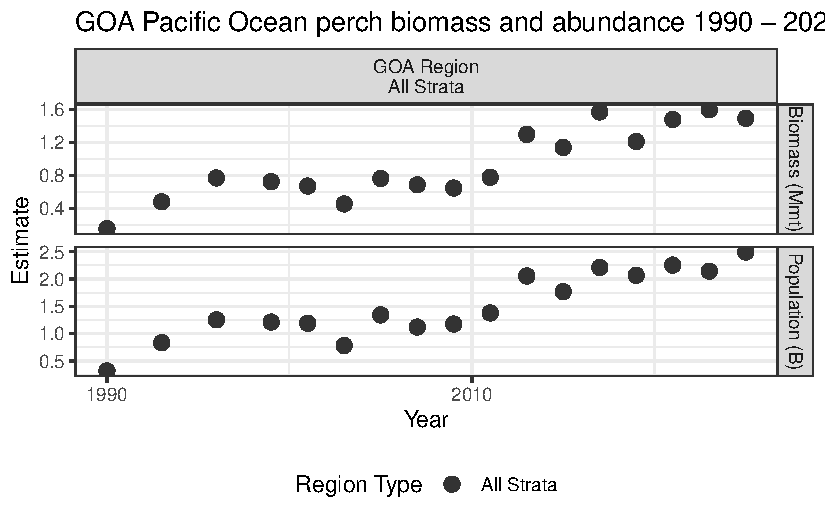
\includegraphics{content/akfin-oracle-sql-r_files/figure-pdf/test-1-plot-1.pdf}

}

\caption{Ex. 1: GOA Pacific Ocean perch biomass and abundance.}

\end{figure}

\hypertarget{ex.-2-ai-rock-sole-size-compositions-and-ridge-plot}{%
\subsection{Ex. 2: AI Rock sole size compositions and ridge
plot}\label{ex.-2-ai-rock-sole-size-compositions-and-ridge-plot}}

Northern and Southern rock sole size composition data from 1991 -- 2022
for the Aleutian Islands, with Ridge plot from
\href{https://cran.r-project.org/web/packages/ggridges/vignettes/introduction.html}{\texttt{ggridges}}.

\begin{Shaded}
\begin{Highlighting}[]
\NormalTok{dat }\OtherTok{\textless{}{-}}\NormalTok{ RODBC}\SpecialCharTok{::}\FunctionTok{sqlQuery}\NormalTok{(}\AttributeTok{channel =}\NormalTok{ channel, }
                       \AttributeTok{query =} 
\StringTok{"WITH FILTERED\_STRATA AS (}
\StringTok{SELECT }
\StringTok{AREA\_ID, }
\StringTok{DESCRIPTION }
\StringTok{FROM GAP\_PRODUCTS.AKFIN\_AREA}
\StringTok{WHERE TYPE = \textquotesingle{}REGION\textquotesingle{} }
\StringTok{AND SURVEY\_DEFINITION\_ID = 52)}
\StringTok{SELECT }
\StringTok{LENGTH\_MM, }
\StringTok{YEAR}
\StringTok{FROM GAP\_PRODUCTS.AKFIN\_SIZECOMP SIZECOMP}
\StringTok{JOIN FILTERED\_STRATA STRATA }
\StringTok{ON STRATA.AREA\_ID = SIZECOMP.AREA\_ID}
\StringTok{WHERE SIZECOMP.SURVEY\_DEFINITION\_ID IN 52 }
\StringTok{AND SIZECOMP.SPECIES\_CODE IN (10261, 10262)"}\NormalTok{)}
\end{Highlighting}
\end{Shaded}

\begin{Shaded}
\begin{Highlighting}[]
\NormalTok{dat0 }\OtherTok{\textless{}{-}}\NormalTok{ dat }\SpecialCharTok{\%\textgreater{}\%} 
\NormalTok{  janitor}\SpecialCharTok{::}\FunctionTok{clean\_names}\NormalTok{() }\SpecialCharTok{\%\textgreater{}\%} 
\NormalTok{  dplyr}\SpecialCharTok{::}\FunctionTok{mutate}\NormalTok{(}\AttributeTok{length\_cm =}\NormalTok{ length\_mm}\SpecialCharTok{/}\DecValTok{10}\NormalTok{)}
\NormalTok{flextable}\SpecialCharTok{::}\FunctionTok{flextable}\NormalTok{(}\FunctionTok{head}\NormalTok{(dat)) }\SpecialCharTok{\%\textgreater{}\%} 
  \FunctionTok{theme\_zebra}\NormalTok{() }\SpecialCharTok{\%\textgreater{}\%}
\NormalTok{    flextable}\SpecialCharTok{::}\FunctionTok{colformat\_num}\NormalTok{(}\AttributeTok{x =}\NormalTok{ ., }\AttributeTok{j =} \StringTok{"YEAR"}\NormalTok{, }\AttributeTok{big.mark =} \StringTok{""}\NormalTok{)}
\end{Highlighting}
\end{Shaded}

\global\setlength{\Oldarrayrulewidth}{\arrayrulewidth}

\global\setlength{\Oldtabcolsep}{\tabcolsep}

\setlength{\tabcolsep}{0pt}

\renewcommand*{\arraystretch}{1.5}



\providecommand{\ascline}[3]{\noalign{\global\arrayrulewidth #1}\arrayrulecolor[HTML]{#2}\cline{#3}}

\begin{longtable}[c]{|p{0.75in}|p{0.75in}}

\caption{Ex. 2: AI Rock sole size compositions and ridge plot.} \\ 


\hhline{>{\arrayrulecolor[HTML]{000000}\global\arrayrulewidth=0pt}->{\arrayrulecolor[HTML]{000000}\global\arrayrulewidth=0pt}-}

\multicolumn{1}{>{\cellcolor[HTML]{CFCFCF}\raggedleft}m{\dimexpr 0.75in+0\tabcolsep}}{\textcolor[HTML]{000000}{\fontsize{11}{11}\selectfont{\textbf{LENGTH\_MM}}}} & \multicolumn{1}{>{\cellcolor[HTML]{CFCFCF}\raggedleft}m{\dimexpr 0.75in+0\tabcolsep}}{\textcolor[HTML]{000000}{\fontsize{11}{11}\selectfont{\textbf{YEAR}}}} \\

\noalign{\global\arrayrulewidth 0pt}\arrayrulecolor[HTML]{000000}

\endhead



\multicolumn{1}{>{\cellcolor[HTML]{EFEFEF}\raggedleft}m{\dimexpr 0.75in+0\tabcolsep}}{\textcolor[HTML]{000000}{\fontsize{11}{11}\selectfont{110}}} & \multicolumn{1}{>{\cellcolor[HTML]{EFEFEF}\raggedleft}m{\dimexpr 0.75in+0\tabcolsep}}{\textcolor[HTML]{000000}{\fontsize{11}{11}\selectfont{1997}}} \\

\noalign{\global\arrayrulewidth 0pt}\arrayrulecolor[HTML]{000000}





\multicolumn{1}{>{\raggedleft}m{\dimexpr 0.75in+0\tabcolsep}}{\textcolor[HTML]{000000}{\fontsize{11}{11}\selectfont{130}}} & \multicolumn{1}{>{\raggedleft}m{\dimexpr 0.75in+0\tabcolsep}}{\textcolor[HTML]{000000}{\fontsize{11}{11}\selectfont{1997}}} \\

\noalign{\global\arrayrulewidth 0pt}\arrayrulecolor[HTML]{000000}





\multicolumn{1}{>{\cellcolor[HTML]{EFEFEF}\raggedleft}m{\dimexpr 0.75in+0\tabcolsep}}{\textcolor[HTML]{000000}{\fontsize{11}{11}\selectfont{140}}} & \multicolumn{1}{>{\cellcolor[HTML]{EFEFEF}\raggedleft}m{\dimexpr 0.75in+0\tabcolsep}}{\textcolor[HTML]{000000}{\fontsize{11}{11}\selectfont{1997}}} \\

\noalign{\global\arrayrulewidth 0pt}\arrayrulecolor[HTML]{000000}





\multicolumn{1}{>{\raggedleft}m{\dimexpr 0.75in+0\tabcolsep}}{\textcolor[HTML]{000000}{\fontsize{11}{11}\selectfont{150}}} & \multicolumn{1}{>{\raggedleft}m{\dimexpr 0.75in+0\tabcolsep}}{\textcolor[HTML]{000000}{\fontsize{11}{11}\selectfont{1997}}} \\

\noalign{\global\arrayrulewidth 0pt}\arrayrulecolor[HTML]{000000}





\multicolumn{1}{>{\cellcolor[HTML]{EFEFEF}\raggedleft}m{\dimexpr 0.75in+0\tabcolsep}}{\textcolor[HTML]{000000}{\fontsize{11}{11}\selectfont{160}}} & \multicolumn{1}{>{\cellcolor[HTML]{EFEFEF}\raggedleft}m{\dimexpr 0.75in+0\tabcolsep}}{\textcolor[HTML]{000000}{\fontsize{11}{11}\selectfont{1997}}} \\

\noalign{\global\arrayrulewidth 0pt}\arrayrulecolor[HTML]{000000}





\multicolumn{1}{>{\raggedleft}m{\dimexpr 0.75in+0\tabcolsep}}{\textcolor[HTML]{000000}{\fontsize{11}{11}\selectfont{170}}} & \multicolumn{1}{>{\raggedleft}m{\dimexpr 0.75in+0\tabcolsep}}{\textcolor[HTML]{000000}{\fontsize{11}{11}\selectfont{1997}}} \\

\noalign{\global\arrayrulewidth 0pt}\arrayrulecolor[HTML]{000000}





\end{longtable}



\arrayrulecolor[HTML]{000000}

\global\setlength{\arrayrulewidth}{\Oldarrayrulewidth}

\global\setlength{\tabcolsep}{\Oldtabcolsep}

\renewcommand*{\arraystretch}{1}

\begin{Shaded}
\begin{Highlighting}[]
\CommentTok{\# install.packages("ggridges")}
\FunctionTok{library}\NormalTok{(ggridges)}
\NormalTok{figure }\OtherTok{\textless{}{-}} 
\NormalTok{  ggplot2}\SpecialCharTok{::}\FunctionTok{ggplot}\NormalTok{(}
    \AttributeTok{data =}\NormalTok{ dat0, }
    \AttributeTok{mapping =} \FunctionTok{aes}\NormalTok{(}\AttributeTok{x =}\NormalTok{ length\_cm, }\AttributeTok{y =} \FunctionTok{as.factor}\NormalTok{(year), }\AttributeTok{fill =} \FunctionTok{stat}\NormalTok{(x))) }\SpecialCharTok{+}
\NormalTok{  ggridges}\SpecialCharTok{::}\FunctionTok{theme\_ridges}\NormalTok{(}\AttributeTok{center\_axis\_labels =} \ConstantTok{TRUE}\NormalTok{) }\SpecialCharTok{+} 
\NormalTok{  ggridges}\SpecialCharTok{::}\FunctionTok{geom\_density\_ridges\_gradient}\NormalTok{(}\AttributeTok{scale =} \DecValTok{4}\NormalTok{, }\AttributeTok{show.legend =} \ConstantTok{FALSE}\NormalTok{) }\SpecialCharTok{+} 
\NormalTok{  ggplot2}\SpecialCharTok{::}\FunctionTok{scale\_y\_discrete}\NormalTok{(}\AttributeTok{name =} \StringTok{"Year"}\NormalTok{, }\AttributeTok{expand =} \FunctionTok{c}\NormalTok{(}\FloatTok{0.01}\NormalTok{, }\DecValTok{0}\NormalTok{)) }\SpecialCharTok{+}
\NormalTok{  ggplot2}\SpecialCharTok{::}\FunctionTok{scale\_x\_continuous}\NormalTok{(}\AttributeTok{name =} \StringTok{"Length (cm)"}\NormalTok{, }\AttributeTok{expand =} \FunctionTok{c}\NormalTok{(}\FloatTok{0.01}\NormalTok{, }\DecValTok{0}\NormalTok{)) }\SpecialCharTok{+}
  \CommentTok{\# ggplot2::scale\_fill\_grey() +}
\NormalTok{  ggplot2}\SpecialCharTok{::}\FunctionTok{labs}\NormalTok{(}\AttributeTok{title =} \StringTok{\textquotesingle{}AI Rock sole Size Compositions 1991 – 2022\textquotesingle{}}\NormalTok{) }

\NormalTok{figure}
\end{Highlighting}
\end{Shaded}

\begin{figure}[H]

{\centering 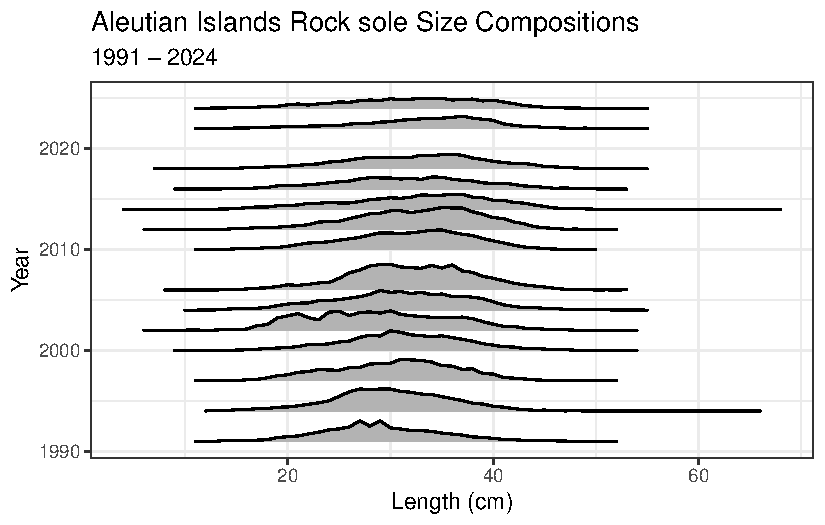
\includegraphics{content/akfin-oracle-sql-r_files/figure-pdf/test-2-plot-1.pdf}

}

\caption{Ex. 2: AI Rock sole size compositions and ridge plot.}

\end{figure}

\hypertarget{ex.-3-ebs-walleye-pollock-age-compositions-and-age-pyramid}{%
\subsection{Ex. 3: EBS Walleye Pollock Age Compositions and Age
Pyramid}\label{ex.-3-ebs-walleye-pollock-age-compositions-and-age-pyramid}}

Walleye pollock age composition for the EBS Standard Area from 1982 --
2022 and the EBS + NW Area from 1987 -- 2022, with age pyramid plot.

\begin{Shaded}
\begin{Highlighting}[]
\NormalTok{dat }\OtherTok{\textless{}{-}}\NormalTok{ RODBC}\SpecialCharTok{::}\FunctionTok{sqlQuery}\NormalTok{(}\AttributeTok{channel =}\NormalTok{ channel, }
                       \AttributeTok{query =} 
\StringTok{"WITH FILTERED\_STRATA AS (}
\StringTok{SELECT }
\StringTok{AREA\_ID, }
\StringTok{DESCRIPTION }
\StringTok{FROM GAP\_PRODUCTS.AKFIN\_AREA}
\StringTok{WHERE TYPE = \textquotesingle{}REGION\textquotesingle{} AND }
\StringTok{SURVEY\_DEFINITION\_ID = 98)}
\StringTok{SELECT }
\StringTok{AGECOMP.AGE, }
\StringTok{AGECOMP.POPULATION\_COUNT, }
\StringTok{AGECOMP.SEX}
\StringTok{FROM GAP\_PRODUCTS.AKFIN\_AGECOMP AGECOMP}
\StringTok{JOIN FILTERED\_STRATA STRATA }
\StringTok{ON STRATA.AREA\_ID = AGECOMP.AREA\_ID}
\StringTok{WHERE SURVEY\_DEFINITION\_ID = 98 }
\StringTok{AND SPECIES\_CODE = 21740}
\StringTok{AND AGE \textgreater{}= 0"}\NormalTok{)}
\end{Highlighting}
\end{Shaded}

\begin{Shaded}
\begin{Highlighting}[]
\NormalTok{dat0 }\OtherTok{\textless{}{-}}\NormalTok{ dat }\SpecialCharTok{\%\textgreater{}\%} 
\NormalTok{  janitor}\SpecialCharTok{::}\FunctionTok{clean\_names}\NormalTok{() }\SpecialCharTok{\%\textgreater{}\%} 
\NormalTok{  dplyr}\SpecialCharTok{::}\FunctionTok{filter}\NormalTok{(sex }\SpecialCharTok{\%in\%} \FunctionTok{c}\NormalTok{(}\DecValTok{1}\NormalTok{,}\DecValTok{2}\NormalTok{)) }\SpecialCharTok{\%\textgreater{}\%}
\NormalTok{  dplyr}\SpecialCharTok{::}\FunctionTok{mutate}\NormalTok{(}
    \AttributeTok{sex =} \FunctionTok{ifelse}\NormalTok{(sex }\SpecialCharTok{==} \DecValTok{1}\NormalTok{, }\StringTok{"M"}\NormalTok{, }\StringTok{"F"}\NormalTok{),}
    \AttributeTok{population\_count =} \CommentTok{\# change male population to negative}
      \FunctionTok{ifelse}\NormalTok{(sex}\SpecialCharTok{==}\StringTok{"M"}\NormalTok{, population\_count}\SpecialCharTok{*}\NormalTok{(}\SpecialCharTok{{-}}\DecValTok{1}\NormalTok{), population\_count}\SpecialCharTok{*}\DecValTok{1}\NormalTok{)}\SpecialCharTok{/}\FloatTok{1e9}\NormalTok{) }

\NormalTok{flextable}\SpecialCharTok{::}\FunctionTok{flextable}\NormalTok{(}\FunctionTok{head}\NormalTok{(dat)) }\SpecialCharTok{\%\textgreater{}\%} \FunctionTok{theme\_zebra}\NormalTok{()}
\end{Highlighting}
\end{Shaded}

\global\setlength{\Oldarrayrulewidth}{\arrayrulewidth}

\global\setlength{\Oldtabcolsep}{\tabcolsep}

\setlength{\tabcolsep}{0pt}

\renewcommand*{\arraystretch}{1.5}



\providecommand{\ascline}[3]{\noalign{\global\arrayrulewidth #1}\arrayrulecolor[HTML]{#2}\cline{#3}}

\begin{longtable}[c]{|p{0.75in}|p{0.75in}|p{0.75in}}

\caption{Ex. 3: EBS Walleye Pollock Age Compositions and Age Pyramid.} \\ 


\hhline{>{\arrayrulecolor[HTML]{000000}\global\arrayrulewidth=0pt}->{\arrayrulecolor[HTML]{000000}\global\arrayrulewidth=0pt}->{\arrayrulecolor[HTML]{000000}\global\arrayrulewidth=0pt}-}

\multicolumn{1}{>{\cellcolor[HTML]{CFCFCF}\raggedleft}m{\dimexpr 0.75in+0\tabcolsep}}{\textcolor[HTML]{000000}{\fontsize{11}{11}\selectfont{\textbf{AGE}}}} & \multicolumn{1}{>{\cellcolor[HTML]{CFCFCF}\raggedleft}m{\dimexpr 0.75in+0\tabcolsep}}{\textcolor[HTML]{000000}{\fontsize{11}{11}\selectfont{\textbf{POPULATION\_COUNT}}}} & \multicolumn{1}{>{\cellcolor[HTML]{CFCFCF}\raggedleft}m{\dimexpr 0.75in+0\tabcolsep}}{\textcolor[HTML]{000000}{\fontsize{11}{11}\selectfont{\textbf{SEX}}}} \\

\noalign{\global\arrayrulewidth 0pt}\arrayrulecolor[HTML]{000000}

\endhead



\multicolumn{1}{>{\cellcolor[HTML]{EFEFEF}\raggedleft}m{\dimexpr 0.75in+0\tabcolsep}}{\textcolor[HTML]{000000}{\fontsize{11}{11}\selectfont{1}}} & \multicolumn{1}{>{\cellcolor[HTML]{EFEFEF}\raggedleft}m{\dimexpr 0.75in+0\tabcolsep}}{\textcolor[HTML]{000000}{\fontsize{11}{11}\selectfont{33,930,956}}} & \multicolumn{1}{>{\cellcolor[HTML]{EFEFEF}\raggedleft}m{\dimexpr 0.75in+0\tabcolsep}}{\textcolor[HTML]{000000}{\fontsize{11}{11}\selectfont{1}}} \\

\noalign{\global\arrayrulewidth 0pt}\arrayrulecolor[HTML]{000000}





\multicolumn{1}{>{\raggedleft}m{\dimexpr 0.75in+0\tabcolsep}}{\textcolor[HTML]{000000}{\fontsize{11}{11}\selectfont{2}}} & \multicolumn{1}{>{\raggedleft}m{\dimexpr 0.75in+0\tabcolsep}}{\textcolor[HTML]{000000}{\fontsize{11}{11}\selectfont{314,043,443}}} & \multicolumn{1}{>{\raggedleft}m{\dimexpr 0.75in+0\tabcolsep}}{\textcolor[HTML]{000000}{\fontsize{11}{11}\selectfont{1}}} \\

\noalign{\global\arrayrulewidth 0pt}\arrayrulecolor[HTML]{000000}





\multicolumn{1}{>{\cellcolor[HTML]{EFEFEF}\raggedleft}m{\dimexpr 0.75in+0\tabcolsep}}{\textcolor[HTML]{000000}{\fontsize{11}{11}\selectfont{3}}} & \multicolumn{1}{>{\cellcolor[HTML]{EFEFEF}\raggedleft}m{\dimexpr 0.75in+0\tabcolsep}}{\textcolor[HTML]{000000}{\fontsize{11}{11}\selectfont{103,452,658}}} & \multicolumn{1}{>{\cellcolor[HTML]{EFEFEF}\raggedleft}m{\dimexpr 0.75in+0\tabcolsep}}{\textcolor[HTML]{000000}{\fontsize{11}{11}\selectfont{1}}} \\

\noalign{\global\arrayrulewidth 0pt}\arrayrulecolor[HTML]{000000}





\multicolumn{1}{>{\raggedleft}m{\dimexpr 0.75in+0\tabcolsep}}{\textcolor[HTML]{000000}{\fontsize{11}{11}\selectfont{4}}} & \multicolumn{1}{>{\raggedleft}m{\dimexpr 0.75in+0\tabcolsep}}{\textcolor[HTML]{000000}{\fontsize{11}{11}\selectfont{47,525,134}}} & \multicolumn{1}{>{\raggedleft}m{\dimexpr 0.75in+0\tabcolsep}}{\textcolor[HTML]{000000}{\fontsize{11}{11}\selectfont{1}}} \\

\noalign{\global\arrayrulewidth 0pt}\arrayrulecolor[HTML]{000000}





\multicolumn{1}{>{\cellcolor[HTML]{EFEFEF}\raggedleft}m{\dimexpr 0.75in+0\tabcolsep}}{\textcolor[HTML]{000000}{\fontsize{11}{11}\selectfont{5}}} & \multicolumn{1}{>{\cellcolor[HTML]{EFEFEF}\raggedleft}m{\dimexpr 0.75in+0\tabcolsep}}{\textcolor[HTML]{000000}{\fontsize{11}{11}\selectfont{203,340,101}}} & \multicolumn{1}{>{\cellcolor[HTML]{EFEFEF}\raggedleft}m{\dimexpr 0.75in+0\tabcolsep}}{\textcolor[HTML]{000000}{\fontsize{11}{11}\selectfont{1}}} \\

\noalign{\global\arrayrulewidth 0pt}\arrayrulecolor[HTML]{000000}





\multicolumn{1}{>{\raggedleft}m{\dimexpr 0.75in+0\tabcolsep}}{\textcolor[HTML]{000000}{\fontsize{11}{11}\selectfont{6}}} & \multicolumn{1}{>{\raggedleft}m{\dimexpr 0.75in+0\tabcolsep}}{\textcolor[HTML]{000000}{\fontsize{11}{11}\selectfont{246,665,076}}} & \multicolumn{1}{>{\raggedleft}m{\dimexpr 0.75in+0\tabcolsep}}{\textcolor[HTML]{000000}{\fontsize{11}{11}\selectfont{1}}} \\

\noalign{\global\arrayrulewidth 0pt}\arrayrulecolor[HTML]{000000}





\end{longtable}



\arrayrulecolor[HTML]{000000}

\global\setlength{\arrayrulewidth}{\Oldarrayrulewidth}

\global\setlength{\tabcolsep}{\Oldtabcolsep}

\renewcommand*{\arraystretch}{1}

\begin{Shaded}
\begin{Highlighting}[]
\NormalTok{figure }\OtherTok{\textless{}{-}}\NormalTok{ ggplot2}\SpecialCharTok{::}\FunctionTok{ggplot}\NormalTok{(}
  \AttributeTok{data =}\NormalTok{ dat0, }
  \AttributeTok{mapping =} 
                 \FunctionTok{aes}\NormalTok{(}\AttributeTok{x =}\NormalTok{ age,}
                     \AttributeTok{y =}\NormalTok{ population\_count, }
                     \AttributeTok{fill =}\NormalTok{ sex)) }\SpecialCharTok{+}
\NormalTok{  ggplot2}\SpecialCharTok{::}\FunctionTok{scale\_fill\_grey}\NormalTok{() }\SpecialCharTok{+}
\NormalTok{  ggplot2}\SpecialCharTok{::}\FunctionTok{geom\_bar}\NormalTok{(}\AttributeTok{stat =} \StringTok{"identity"}\NormalTok{) }\SpecialCharTok{+}
\NormalTok{  ggplot2}\SpecialCharTok{::}\FunctionTok{coord\_flip}\NormalTok{() }\SpecialCharTok{+}
\NormalTok{  ggplot2}\SpecialCharTok{::}\FunctionTok{scale\_x\_continuous}\NormalTok{(}\AttributeTok{name =} \StringTok{"Age"}\NormalTok{) }\SpecialCharTok{+}
\NormalTok{  ggplot2}\SpecialCharTok{::}\FunctionTok{scale\_y\_continuous}\NormalTok{(}\AttributeTok{name =} \StringTok{"Population (billions)"}\NormalTok{, }\AttributeTok{labels =}\NormalTok{ abs) }\SpecialCharTok{+}
\NormalTok{  ggplot2}\SpecialCharTok{::}\FunctionTok{ggtitle}\NormalTok{(}\AttributeTok{label =} \StringTok{"EBS Walleye Pollock Age Compositions 1982 – 2022"}\NormalTok{)  }\SpecialCharTok{+} 
\NormalTok{  ggplot2}\SpecialCharTok{::}\FunctionTok{guides}\NormalTok{(}\AttributeTok{fill =} \FunctionTok{guide\_legend}\NormalTok{(}\AttributeTok{title =} \StringTok{"Sex"}\NormalTok{))}\SpecialCharTok{+}
\NormalTok{  ggplot2}\SpecialCharTok{::}\FunctionTok{theme\_bw}\NormalTok{()}

\NormalTok{figure}
\end{Highlighting}
\end{Shaded}

\begin{figure}[H]

{\centering 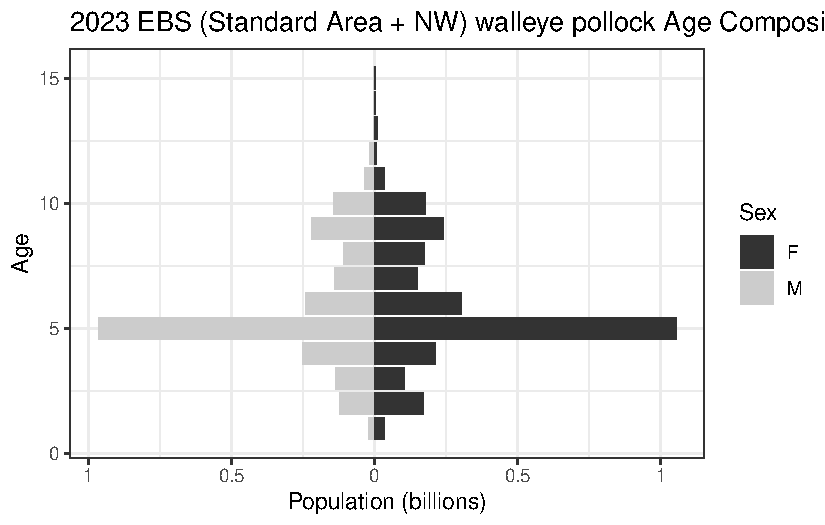
\includegraphics{content/akfin-oracle-sql-r_files/figure-pdf/test-3-plot-1.pdf}

}

\caption{Ex. 3: EBS Walleye Pollock Age Compositions and Age Pyramid.}

\end{figure}

\hypertarget{ex.-4-nbs-pacific-cod-biomass-and-abundance}{%
\subsection{Ex. 4: NBS Pacific cod biomass and
abundance}\label{ex.-4-nbs-pacific-cod-biomass-and-abundance}}

Pacific cod biomass and abundance data for the NBS by stratum.

\begin{Shaded}
\begin{Highlighting}[]
\NormalTok{dat }\OtherTok{\textless{}{-}}\NormalTok{ RODBC}\SpecialCharTok{::}\FunctionTok{sqlQuery}\NormalTok{(}\AttributeTok{channel =}\NormalTok{ channel, }
                       \AttributeTok{query =} 
\StringTok{"WITH FILTERED\_STRATA AS (}
\StringTok{SELECT }
\StringTok{AREA\_ID, }
\StringTok{AREA\_NAME, }
\StringTok{DESCRIPTION }
\StringTok{FROM GAP\_PRODUCTS.AKFIN\_AREA}
\StringTok{WHERE TYPE in (\textquotesingle{}STRATUM\textquotesingle{}) AND }
\StringTok{SURVEY\_DEFINITION\_ID = 143) }
\StringTok{SELECT }
\StringTok{BIOMASS.BIOMASS\_MT, }
\StringTok{BIOMASS.POPULATION\_COUNT, }
\StringTok{BIOMASS.YEAR, }
\StringTok{STRATA.AREA\_NAME}
\StringTok{FROM GAP\_PRODUCTS.AKFIN\_BIOMASS BIOMASS }
\StringTok{JOIN FILTERED\_STRATA STRATA }
\StringTok{ON STRATA.AREA\_ID = BIOMASS.AREA\_ID}
\StringTok{WHERE BIOMASS.SURVEY\_DEFINITION\_ID IN 143 }
\StringTok{AND BIOMASS.SPECIES\_CODE = 21720"}\NormalTok{)}
\end{Highlighting}
\end{Shaded}

\begin{Shaded}
\begin{Highlighting}[]
\NormalTok{dat0 }\OtherTok{\textless{}{-}}\NormalTok{ dat }\SpecialCharTok{\%\textgreater{}\%} 
\NormalTok{  janitor}\SpecialCharTok{::}\FunctionTok{clean\_names}\NormalTok{() }\SpecialCharTok{\%\textgreater{}\%} 
\NormalTok{  dplyr}\SpecialCharTok{::}\FunctionTok{select}\NormalTok{(biomass\_mt, population\_count, year, }\AttributeTok{area =}\NormalTok{ area\_name) }\SpecialCharTok{\%\textgreater{}\%}
  \FunctionTok{pivot\_longer}\NormalTok{(}\AttributeTok{cols =} \FunctionTok{c}\NormalTok{(}\StringTok{"biomass\_mt"}\NormalTok{, }\StringTok{"population\_count"}\NormalTok{), }
               \AttributeTok{names\_to =} \StringTok{"var"}\NormalTok{, }
               \AttributeTok{values\_to =} \StringTok{"val"}\NormalTok{) }\SpecialCharTok{\%\textgreater{}\%} 
\NormalTok{  dplyr}\SpecialCharTok{::}\FunctionTok{mutate}\NormalTok{(}
    \AttributeTok{val =} \FunctionTok{ifelse}\NormalTok{(var }\SpecialCharTok{==} \StringTok{"biomass\_mt"}\NormalTok{, val}\SpecialCharTok{/}\FloatTok{1e6}\NormalTok{, val}\SpecialCharTok{/}\FloatTok{1e9}\NormalTok{), }
    \AttributeTok{var =} \FunctionTok{ifelse}\NormalTok{(var }\SpecialCharTok{==} \StringTok{"biomass\_mt"}\NormalTok{, }\StringTok{"Biomass (Mmt)"}\NormalTok{, }\StringTok{"Population (B)"}\NormalTok{), }
    \AttributeTok{area =} \FunctionTok{factor}\NormalTok{(area, }\AttributeTok{levels =} \FunctionTok{unique}\NormalTok{(area), }\AttributeTok{labels =} \FunctionTok{unique}\NormalTok{(area), }\AttributeTok{ordered =} \ConstantTok{TRUE}\NormalTok{))}
\NormalTok{flextable}\SpecialCharTok{::}\FunctionTok{flextable}\NormalTok{(}\FunctionTok{head}\NormalTok{(dat)) }\SpecialCharTok{\%\textgreater{}\%} 
  \FunctionTok{theme\_zebra}\NormalTok{() }\SpecialCharTok{\%\textgreater{}\%}
\NormalTok{  flextable}\SpecialCharTok{::}\FunctionTok{colformat\_num}\NormalTok{(}\AttributeTok{x =}\NormalTok{ ., }\AttributeTok{j =} \StringTok{"YEAR"}\NormalTok{, }\AttributeTok{big.mark =} \StringTok{""}\NormalTok{)}
\end{Highlighting}
\end{Shaded}

\global\setlength{\Oldarrayrulewidth}{\arrayrulewidth}

\global\setlength{\Oldtabcolsep}{\tabcolsep}

\setlength{\tabcolsep}{0pt}

\renewcommand*{\arraystretch}{1.5}



\providecommand{\ascline}[3]{\noalign{\global\arrayrulewidth #1}\arrayrulecolor[HTML]{#2}\cline{#3}}

\begin{longtable}[c]{|p{0.75in}|p{0.75in}|p{0.75in}|p{0.75in}}

\caption{Ex. 4: NBS Pacific cod biomass and abundance.} \\ 


\hhline{>{\arrayrulecolor[HTML]{000000}\global\arrayrulewidth=0pt}->{\arrayrulecolor[HTML]{000000}\global\arrayrulewidth=0pt}->{\arrayrulecolor[HTML]{000000}\global\arrayrulewidth=0pt}->{\arrayrulecolor[HTML]{000000}\global\arrayrulewidth=0pt}-}

\multicolumn{1}{>{\cellcolor[HTML]{CFCFCF}\raggedleft}m{\dimexpr 0.75in+0\tabcolsep}}{\textcolor[HTML]{000000}{\fontsize{11}{11}\selectfont{\textbf{BIOMASS\_MT}}}} & \multicolumn{1}{>{\cellcolor[HTML]{CFCFCF}\raggedleft}m{\dimexpr 0.75in+0\tabcolsep}}{\textcolor[HTML]{000000}{\fontsize{11}{11}\selectfont{\textbf{POPULATION\_COUNT}}}} & \multicolumn{1}{>{\cellcolor[HTML]{CFCFCF}\raggedleft}m{\dimexpr 0.75in+0\tabcolsep}}{\textcolor[HTML]{000000}{\fontsize{11}{11}\selectfont{\textbf{YEAR}}}} & \multicolumn{1}{>{\cellcolor[HTML]{CFCFCF}\raggedright}m{\dimexpr 0.75in+0\tabcolsep}}{\textcolor[HTML]{000000}{\fontsize{11}{11}\selectfont{\textbf{AREA\_NAME}}}} \\

\noalign{\global\arrayrulewidth 0pt}\arrayrulecolor[HTML]{000000}

\endhead



\multicolumn{1}{>{\cellcolor[HTML]{EFEFEF}\raggedleft}m{\dimexpr 0.75in+0\tabcolsep}}{\textcolor[HTML]{000000}{\fontsize{11}{11}\selectfont{7,462.559}}} & \multicolumn{1}{>{\cellcolor[HTML]{EFEFEF}\raggedleft}m{\dimexpr 0.75in+0\tabcolsep}}{\textcolor[HTML]{000000}{\fontsize{11}{11}\selectfont{4,724,153}}} & \multicolumn{1}{>{\cellcolor[HTML]{EFEFEF}\raggedleft}m{\dimexpr 0.75in+0\tabcolsep}}{\textcolor[HTML]{000000}{\fontsize{11}{11}\selectfont{2010}}} & \multicolumn{1}{>{\cellcolor[HTML]{EFEFEF}\raggedright}m{\dimexpr 0.75in+0\tabcolsep}}{\textcolor[HTML]{000000}{\fontsize{11}{11}\selectfont{Inner\ Domain}}} \\

\noalign{\global\arrayrulewidth 0pt}\arrayrulecolor[HTML]{000000}





\multicolumn{1}{>{\raggedleft}m{\dimexpr 0.75in+0\tabcolsep}}{\textcolor[HTML]{000000}{\fontsize{11}{11}\selectfont{95,849.983}}} & \multicolumn{1}{>{\raggedleft}m{\dimexpr 0.75in+0\tabcolsep}}{\textcolor[HTML]{000000}{\fontsize{11}{11}\selectfont{68,767,498}}} & \multicolumn{1}{>{\raggedleft}m{\dimexpr 0.75in+0\tabcolsep}}{\textcolor[HTML]{000000}{\fontsize{11}{11}\selectfont{2021}}} & \multicolumn{1}{>{\raggedright}m{\dimexpr 0.75in+0\tabcolsep}}{\textcolor[HTML]{000000}{\fontsize{11}{11}\selectfont{Inner\ Domain}}} \\

\noalign{\global\arrayrulewidth 0pt}\arrayrulecolor[HTML]{000000}





\multicolumn{1}{>{\cellcolor[HTML]{EFEFEF}\raggedleft}m{\dimexpr 0.75in+0\tabcolsep}}{\textcolor[HTML]{000000}{\fontsize{11}{11}\selectfont{107,096.730}}} & \multicolumn{1}{>{\cellcolor[HTML]{EFEFEF}\raggedleft}m{\dimexpr 0.75in+0\tabcolsep}}{\textcolor[HTML]{000000}{\fontsize{11}{11}\selectfont{102,734,142}}} & \multicolumn{1}{>{\cellcolor[HTML]{EFEFEF}\raggedleft}m{\dimexpr 0.75in+0\tabcolsep}}{\textcolor[HTML]{000000}{\fontsize{11}{11}\selectfont{2019}}} & \multicolumn{1}{>{\cellcolor[HTML]{EFEFEF}\raggedright}m{\dimexpr 0.75in+0\tabcolsep}}{\textcolor[HTML]{000000}{\fontsize{11}{11}\selectfont{Inner\ Domain}}} \\

\noalign{\global\arrayrulewidth 0pt}\arrayrulecolor[HTML]{000000}





\multicolumn{1}{>{\raggedleft}m{\dimexpr 0.75in+0\tabcolsep}}{\textcolor[HTML]{000000}{\fontsize{11}{11}\selectfont{132,490.152}}} & \multicolumn{1}{>{\raggedleft}m{\dimexpr 0.75in+0\tabcolsep}}{\textcolor[HTML]{000000}{\fontsize{11}{11}\selectfont{66,187,245}}} & \multicolumn{1}{>{\raggedleft}m{\dimexpr 0.75in+0\tabcolsep}}{\textcolor[HTML]{000000}{\fontsize{11}{11}\selectfont{2017}}} & \multicolumn{1}{>{\raggedright}m{\dimexpr 0.75in+0\tabcolsep}}{\textcolor[HTML]{000000}{\fontsize{11}{11}\selectfont{Inner\ Domain}}} \\

\noalign{\global\arrayrulewidth 0pt}\arrayrulecolor[HTML]{000000}





\multicolumn{1}{>{\cellcolor[HTML]{EFEFEF}\raggedleft}m{\dimexpr 0.75in+0\tabcolsep}}{\textcolor[HTML]{000000}{\fontsize{11}{11}\selectfont{96,500.697}}} & \multicolumn{1}{>{\cellcolor[HTML]{EFEFEF}\raggedleft}m{\dimexpr 0.75in+0\tabcolsep}}{\textcolor[HTML]{000000}{\fontsize{11}{11}\selectfont{60,433,135}}} & \multicolumn{1}{>{\cellcolor[HTML]{EFEFEF}\raggedleft}m{\dimexpr 0.75in+0\tabcolsep}}{\textcolor[HTML]{000000}{\fontsize{11}{11}\selectfont{2022}}} & \multicolumn{1}{>{\cellcolor[HTML]{EFEFEF}\raggedright}m{\dimexpr 0.75in+0\tabcolsep}}{\textcolor[HTML]{000000}{\fontsize{11}{11}\selectfont{Inner\ Domain}}} \\

\noalign{\global\arrayrulewidth 0pt}\arrayrulecolor[HTML]{000000}





\multicolumn{1}{>{\raggedleft}m{\dimexpr 0.75in+0\tabcolsep}}{\textcolor[HTML]{000000}{\fontsize{11}{11}\selectfont{147,971.454}}} & \multicolumn{1}{>{\raggedleft}m{\dimexpr 0.75in+0\tabcolsep}}{\textcolor[HTML]{000000}{\fontsize{11}{11}\selectfont{65,078,489}}} & \multicolumn{1}{>{\raggedleft}m{\dimexpr 0.75in+0\tabcolsep}}{\textcolor[HTML]{000000}{\fontsize{11}{11}\selectfont{2017}}} & \multicolumn{1}{>{\raggedright}m{\dimexpr 0.75in+0\tabcolsep}}{\textcolor[HTML]{000000}{\fontsize{11}{11}\selectfont{Inner\ Domain}}} \\

\noalign{\global\arrayrulewidth 0pt}\arrayrulecolor[HTML]{000000}





\end{longtable}



\arrayrulecolor[HTML]{000000}

\global\setlength{\arrayrulewidth}{\Oldarrayrulewidth}

\global\setlength{\tabcolsep}{\Oldtabcolsep}

\renewcommand*{\arraystretch}{1}

\begin{Shaded}
\begin{Highlighting}[]
\NormalTok{figure }\OtherTok{\textless{}{-}}\NormalTok{ ggplot2}\SpecialCharTok{::}\FunctionTok{ggplot}\NormalTok{(}
  \AttributeTok{dat =}\NormalTok{ dat0, }
  \AttributeTok{mapping =} \FunctionTok{aes}\NormalTok{(}\AttributeTok{y =}\NormalTok{ val, }\AttributeTok{x =}\NormalTok{ year, }\AttributeTok{fill =}\NormalTok{ area))  }\SpecialCharTok{+} 
\NormalTok{  ggplot2}\SpecialCharTok{::}\FunctionTok{geom\_bar}\NormalTok{(}\AttributeTok{position=}\StringTok{"stack"}\NormalTok{, }\AttributeTok{stat=}\StringTok{"identity"}\NormalTok{) }\SpecialCharTok{+}  
\NormalTok{  ggplot2}\SpecialCharTok{::}\FunctionTok{facet\_grid}\NormalTok{(}\AttributeTok{rows =} \FunctionTok{vars}\NormalTok{(var), }\AttributeTok{scales =} \StringTok{"free\_y"}\NormalTok{) }\SpecialCharTok{+}
\NormalTok{  ggplot2}\SpecialCharTok{::}\FunctionTok{scale\_y\_continuous}\NormalTok{(}\AttributeTok{name =} \StringTok{"Estimate"}\NormalTok{, }\AttributeTok{labels =}\NormalTok{ comma) }\SpecialCharTok{+}
\NormalTok{  ggplot2}\SpecialCharTok{::}\FunctionTok{scale\_x\_continuous}\NormalTok{(}\AttributeTok{name =} \StringTok{"Year"}\NormalTok{, }\AttributeTok{breaks =} \FunctionTok{unique}\NormalTok{(dat0}\SpecialCharTok{$}\NormalTok{year)) }\SpecialCharTok{+}
\NormalTok{  ggplot2}\SpecialCharTok{::}\FunctionTok{labs}\NormalTok{(}\AttributeTok{title =} \StringTok{\textquotesingle{}NBS Pacific cod biomass and abundance by stratum\textquotesingle{}}\NormalTok{)  }\SpecialCharTok{+} 
\NormalTok{  ggplot2}\SpecialCharTok{::}\FunctionTok{guides}\NormalTok{(}\AttributeTok{fill=}\FunctionTok{guide\_legend}\NormalTok{(}\AttributeTok{title =} \StringTok{"Region Type"}\NormalTok{))}\SpecialCharTok{+}
\NormalTok{  ggplot2}\SpecialCharTok{::}\FunctionTok{scale\_fill\_grey}\NormalTok{() }\SpecialCharTok{+}
\NormalTok{  ggplot2}\SpecialCharTok{::}\FunctionTok{theme\_bw}\NormalTok{() }\SpecialCharTok{+}
\NormalTok{  ggplot2}\SpecialCharTok{::}\FunctionTok{theme}\NormalTok{(}\AttributeTok{legend.direction =} \StringTok{"horizontal"}\NormalTok{, }
                 \AttributeTok{legend.position =} \StringTok{"bottom"}\NormalTok{)}

\NormalTok{figure}
\end{Highlighting}
\end{Shaded}

\begin{figure}[H]

{\centering 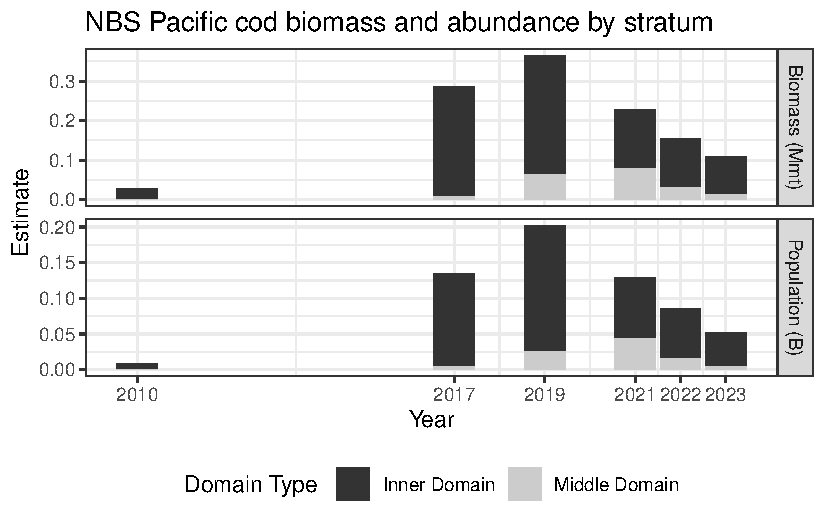
\includegraphics{content/akfin-oracle-sql-r_files/figure-pdf/test-4-fig-1.pdf}

}

\caption{Ex. 4: NBS Pacific cod biomass and abundance.}

\end{figure}

\hypertarget{ex.-5-goa-pacific-ocean-perch-biomass-and-line-plot}{%
\subsection{Ex. 5: GOA Pacific Ocean perch biomass and line
plot}\label{ex.-5-goa-pacific-ocean-perch-biomass-and-line-plot}}

Pacific Ocean perch biomass totals for GOA between 1984-2021 from
\texttt{GAP\_PRODUCTS.AKFIN\_BIOMASS}

\begin{Shaded}
\begin{Highlighting}[]
\NormalTok{dat }\OtherTok{\textless{}{-}}\NormalTok{ RODBC}\SpecialCharTok{::}\FunctionTok{sqlQuery}\NormalTok{(}\AttributeTok{channel =}\NormalTok{ channel, }
                       \AttributeTok{query =} 
\StringTok{"SELECT }
\StringTok{SURVEY\_DEFINITION\_ID, }
\StringTok{BIOMASS\_MT, }
\StringTok{YEAR}
\StringTok{FROM GAP\_PRODUCTS.AKFIN\_BIOMASS}
\StringTok{WHERE SPECIES\_CODE = 30060 }
\StringTok{AND SURVEY\_DEFINITION\_ID = 47 }
\StringTok{AND AREA\_ID = 99903 }
\StringTok{AND YEAR BETWEEN 1984 AND 2021;"}\NormalTok{) }\SpecialCharTok{\%\textgreater{}\%} 
\NormalTok{  janitor}\SpecialCharTok{::}\FunctionTok{clean\_names}\NormalTok{() }\SpecialCharTok{\%\textgreater{}\%} 
\NormalTok{  dplyr}\SpecialCharTok{::}\FunctionTok{mutate}\NormalTok{(}\AttributeTok{biomass\_mt =}\NormalTok{ biomass\_mt}\SpecialCharTok{/}\DecValTok{1000}\NormalTok{)}
\end{Highlighting}
\end{Shaded}

\begin{Shaded}
\begin{Highlighting}[]
\NormalTok{a\_mean }\OtherTok{\textless{}{-}}\NormalTok{ dat }\SpecialCharTok{\%\textgreater{}\%} 
\NormalTok{  dplyr}\SpecialCharTok{::}\FunctionTok{group\_by}\NormalTok{(survey\_definition\_id) }\SpecialCharTok{\%\textgreater{}\%} 
\NormalTok{  dplyr}\SpecialCharTok{::}\FunctionTok{summarise}\NormalTok{(}\AttributeTok{biomass\_mt =} \FunctionTok{mean}\NormalTok{(biomass\_mt, }\AttributeTok{na.rm =} \ConstantTok{TRUE}\NormalTok{), }
                   \AttributeTok{minyr =} \FunctionTok{min}\NormalTok{(year, }\AttributeTok{na.rm =} \ConstantTok{TRUE}\NormalTok{), }
                   \AttributeTok{maxyr =} \FunctionTok{max}\NormalTok{(year, }\AttributeTok{na.rm =} \ConstantTok{TRUE}\NormalTok{)) }
\NormalTok{flextable}\SpecialCharTok{::}\FunctionTok{flextable}\NormalTok{(}\FunctionTok{head}\NormalTok{(dat)) }\SpecialCharTok{\%\textgreater{}\%}
  \FunctionTok{theme\_zebra}\NormalTok{() }\SpecialCharTok{\%\textgreater{}\%}
\NormalTok{  flextable}\SpecialCharTok{::}\FunctionTok{colformat\_num}\NormalTok{(}\AttributeTok{x =}\NormalTok{ ., }\AttributeTok{j =} \StringTok{"year"}\NormalTok{, }\AttributeTok{big.mark =} \StringTok{""}\NormalTok{)}
\end{Highlighting}
\end{Shaded}

\global\setlength{\Oldarrayrulewidth}{\arrayrulewidth}

\global\setlength{\Oldtabcolsep}{\tabcolsep}

\setlength{\tabcolsep}{0pt}

\renewcommand*{\arraystretch}{1.5}



\providecommand{\ascline}[3]{\noalign{\global\arrayrulewidth #1}\arrayrulecolor[HTML]{#2}\cline{#3}}

\begin{longtable}[c]{|p{0.75in}|p{0.75in}|p{0.75in}}

\caption{Ex. 5: GOA Pacific Ocean perch biomass and line plot.} \\ 


\hhline{>{\arrayrulecolor[HTML]{000000}\global\arrayrulewidth=0pt}->{\arrayrulecolor[HTML]{000000}\global\arrayrulewidth=0pt}->{\arrayrulecolor[HTML]{000000}\global\arrayrulewidth=0pt}-}

\multicolumn{1}{>{\cellcolor[HTML]{CFCFCF}\raggedleft}m{\dimexpr 0.75in+0\tabcolsep}}{\textcolor[HTML]{000000}{\fontsize{11}{11}\selectfont{\textbf{survey\_definition\_id}}}} & \multicolumn{1}{>{\cellcolor[HTML]{CFCFCF}\raggedleft}m{\dimexpr 0.75in+0\tabcolsep}}{\textcolor[HTML]{000000}{\fontsize{11}{11}\selectfont{\textbf{biomass\_mt}}}} & \multicolumn{1}{>{\cellcolor[HTML]{CFCFCF}\raggedleft}m{\dimexpr 0.75in+0\tabcolsep}}{\textcolor[HTML]{000000}{\fontsize{11}{11}\selectfont{\textbf{year}}}} \\

\noalign{\global\arrayrulewidth 0pt}\arrayrulecolor[HTML]{000000}

\endhead



\multicolumn{1}{>{\cellcolor[HTML]{EFEFEF}\raggedleft}m{\dimexpr 0.75in+0\tabcolsep}}{\textcolor[HTML]{000000}{\fontsize{11}{11}\selectfont{47}}} & \multicolumn{1}{>{\cellcolor[HTML]{EFEFEF}\raggedleft}m{\dimexpr 0.75in+0\tabcolsep}}{\textcolor[HTML]{000000}{\fontsize{11}{11}\selectfont{483.6226}}} & \multicolumn{1}{>{\cellcolor[HTML]{EFEFEF}\raggedleft}m{\dimexpr 0.75in+0\tabcolsep}}{\textcolor[HTML]{000000}{\fontsize{11}{11}\selectfont{1993}}} \\

\noalign{\global\arrayrulewidth 0pt}\arrayrulecolor[HTML]{000000}





\multicolumn{1}{>{\raggedleft}m{\dimexpr 0.75in+0\tabcolsep}}{\textcolor[HTML]{000000}{\fontsize{11}{11}\selectfont{47}}} & \multicolumn{1}{>{\raggedleft}m{\dimexpr 0.75in+0\tabcolsep}}{\textcolor[HTML]{000000}{\fontsize{11}{11}\selectfont{771.4128}}} & \multicolumn{1}{>{\raggedleft}m{\dimexpr 0.75in+0\tabcolsep}}{\textcolor[HTML]{000000}{\fontsize{11}{11}\selectfont{1996}}} \\

\noalign{\global\arrayrulewidth 0pt}\arrayrulecolor[HTML]{000000}





\multicolumn{1}{>{\cellcolor[HTML]{EFEFEF}\raggedleft}m{\dimexpr 0.75in+0\tabcolsep}}{\textcolor[HTML]{000000}{\fontsize{11}{11}\selectfont{47}}} & \multicolumn{1}{>{\cellcolor[HTML]{EFEFEF}\raggedleft}m{\dimexpr 0.75in+0\tabcolsep}}{\textcolor[HTML]{000000}{\fontsize{11}{11}\selectfont{727.0635}}} & \multicolumn{1}{>{\cellcolor[HTML]{EFEFEF}\raggedleft}m{\dimexpr 0.75in+0\tabcolsep}}{\textcolor[HTML]{000000}{\fontsize{11}{11}\selectfont{1999}}} \\

\noalign{\global\arrayrulewidth 0pt}\arrayrulecolor[HTML]{000000}





\multicolumn{1}{>{\raggedleft}m{\dimexpr 0.75in+0\tabcolsep}}{\textcolor[HTML]{000000}{\fontsize{11}{11}\selectfont{47}}} & \multicolumn{1}{>{\raggedleft}m{\dimexpr 0.75in+0\tabcolsep}}{\textcolor[HTML]{000000}{\fontsize{11}{11}\selectfont{673.1551}}} & \multicolumn{1}{>{\raggedleft}m{\dimexpr 0.75in+0\tabcolsep}}{\textcolor[HTML]{000000}{\fontsize{11}{11}\selectfont{2001}}} \\

\noalign{\global\arrayrulewidth 0pt}\arrayrulecolor[HTML]{000000}





\multicolumn{1}{>{\cellcolor[HTML]{EFEFEF}\raggedleft}m{\dimexpr 0.75in+0\tabcolsep}}{\textcolor[HTML]{000000}{\fontsize{11}{11}\selectfont{47}}} & \multicolumn{1}{>{\cellcolor[HTML]{EFEFEF}\raggedleft}m{\dimexpr 0.75in+0\tabcolsep}}{\textcolor[HTML]{000000}{\fontsize{11}{11}\selectfont{457.4216}}} & \multicolumn{1}{>{\cellcolor[HTML]{EFEFEF}\raggedleft}m{\dimexpr 0.75in+0\tabcolsep}}{\textcolor[HTML]{000000}{\fontsize{11}{11}\selectfont{2003}}} \\

\noalign{\global\arrayrulewidth 0pt}\arrayrulecolor[HTML]{000000}





\multicolumn{1}{>{\raggedleft}m{\dimexpr 0.75in+0\tabcolsep}}{\textcolor[HTML]{000000}{\fontsize{11}{11}\selectfont{47}}} & \multicolumn{1}{>{\raggedleft}m{\dimexpr 0.75in+0\tabcolsep}}{\textcolor[HTML]{000000}{\fontsize{11}{11}\selectfont{764.9014}}} & \multicolumn{1}{>{\raggedleft}m{\dimexpr 0.75in+0\tabcolsep}}{\textcolor[HTML]{000000}{\fontsize{11}{11}\selectfont{2005}}} \\

\noalign{\global\arrayrulewidth 0pt}\arrayrulecolor[HTML]{000000}





\end{longtable}



\arrayrulecolor[HTML]{000000}

\global\setlength{\arrayrulewidth}{\Oldarrayrulewidth}

\global\setlength{\tabcolsep}{\Oldtabcolsep}

\renewcommand*{\arraystretch}{1}

\begin{Shaded}
\begin{Highlighting}[]
\NormalTok{figure }\OtherTok{\textless{}{-}}
  \FunctionTok{ggplot}\NormalTok{(}\AttributeTok{data =}\NormalTok{ dat, }
         \AttributeTok{mapping =} \FunctionTok{aes}\NormalTok{(}\AttributeTok{x =}\NormalTok{ year, }
                       \AttributeTok{y =}\NormalTok{ biomass\_mt)) }\SpecialCharTok{+}
\NormalTok{  ggplot2}\SpecialCharTok{::}\FunctionTok{geom\_point}\NormalTok{(}\AttributeTok{size =} \FloatTok{2.5}\NormalTok{, }\AttributeTok{color =} \StringTok{"grey40"}\NormalTok{) }\SpecialCharTok{+} 
\NormalTok{  ggplot2}\SpecialCharTok{::}\FunctionTok{scale\_x\_continuous}\NormalTok{(}
    \AttributeTok{name =} \StringTok{"Year"}\NormalTok{, }
    \AttributeTok{labels =}\NormalTok{ scales}\SpecialCharTok{::}\FunctionTok{label\_number}\NormalTok{(}
      \AttributeTok{accuracy =} \DecValTok{1}\NormalTok{, }
      \AttributeTok{big.mark =} \StringTok{""}\NormalTok{))   }\SpecialCharTok{+}
\NormalTok{  ggplot2}\SpecialCharTok{::}\FunctionTok{scale\_y\_continuous}\NormalTok{(}
    \AttributeTok{name =} \StringTok{"Biomass (Kmt)"}\NormalTok{, }
    \AttributeTok{labels =}\NormalTok{ comma) }\SpecialCharTok{+}
\NormalTok{  ggplot2}\SpecialCharTok{::}\FunctionTok{geom\_segment}\NormalTok{(}
    \AttributeTok{data =}\NormalTok{ a\_mean,}
    \AttributeTok{mapping =} \FunctionTok{aes}\NormalTok{(}\AttributeTok{x =}\NormalTok{ minyr, }
                  \AttributeTok{xend =}\NormalTok{ maxyr, }
                  \AttributeTok{y =}\NormalTok{ biomass\_mt, }
                  \AttributeTok{yend =}\NormalTok{ biomass\_mt),}
    \AttributeTok{linetype =} \StringTok{"dashed"}\NormalTok{, }
    \AttributeTok{linewidth =} \DecValTok{2}\NormalTok{) }\SpecialCharTok{+}
\NormalTok{  ggplot2}\SpecialCharTok{::}\FunctionTok{ggtitle}\NormalTok{(}
    \AttributeTok{label =} \StringTok{"GOA Pacific Ocean Perch Biomass 1984{-}2021"}\NormalTok{, }
    \AttributeTok{subtitle =} \FunctionTok{paste0}\NormalTok{(}\StringTok{"Mean = "}\NormalTok{, }
                      \FunctionTok{formatC}\NormalTok{(}\AttributeTok{x =}\NormalTok{ a\_mean}\SpecialCharTok{$}\NormalTok{biomass\_mt, }
                              \AttributeTok{digits =} \DecValTok{2}\NormalTok{, }
                              \AttributeTok{big.mark =} \StringTok{","}\NormalTok{, }
                              \AttributeTok{format =} \StringTok{"f"}\NormalTok{), }
                      \StringTok{" Kmt"}\NormalTok{)) }\SpecialCharTok{+}
\NormalTok{  ggplot2}\SpecialCharTok{::}\FunctionTok{theme\_bw}\NormalTok{()}

\NormalTok{figure}
\end{Highlighting}
\end{Shaded}

\begin{figure}[H]

{\centering 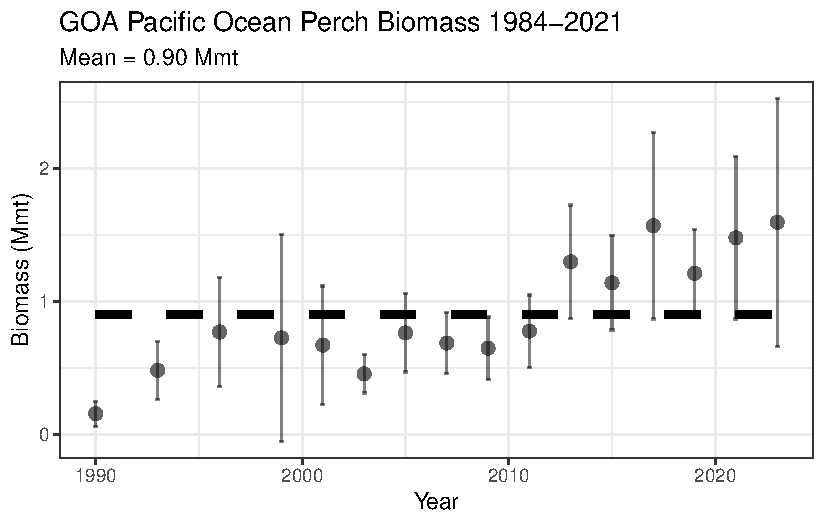
\includegraphics{content/akfin-oracle-sql-r_files/figure-pdf/test-5-fig-1.pdf}

}

\caption{Ex. 5: GOA Pacific Ocean perch biomass and line plot.}

\end{figure}

\hypertarget{ex.-6-ebs-pacific-ocean-perch-cpue-and-akgfmaps-map}{%
\subsection{\texorpdfstring{Ex. 6: EBS Pacific Ocean perch CPUE and
\href{https://github.com/afsc-gap-products/akgfmaps}{\texttt{akgfmaps}}
map}{Ex. 6: EBS Pacific Ocean perch CPUE and akgfmaps map}}\label{ex.-6-ebs-pacific-ocean-perch-cpue-and-akgfmaps-map}}

Pacific Ocean perch catch-per-unit-effort estimates for EBS in 2021 from
\texttt{GAP\_PRODUCTS.AKFIN\_CPUE} and map constructed using
\href{https://github.com/afsc-gap-products/akgfmaps}{\texttt{akgfmaps}}.
Here, we'll use AKFIN HAUL and CRUISES data also included in this repo,
for convenience, though they are very similar to their \texttt{RACEBASE}
analogs.

\begin{Shaded}
\begin{Highlighting}[]
\NormalTok{dat }\OtherTok{\textless{}{-}}\NormalTok{ RODBC}\SpecialCharTok{::}\FunctionTok{sqlQuery}\NormalTok{(}\AttributeTok{channel =}\NormalTok{ channel, }
                       \AttributeTok{query =} 
\StringTok{"SELECT }
\StringTok{(cp.CPUE\_KGKM2/100) CPUE\_KGHA, {-}{-} akgfmaps is expecting hectares}
\StringTok{hh.LATITUDE\_DD\_START LATITUDE,}
\StringTok{hh.LONGITUDE\_DD\_START LONGITUDE}

\StringTok{FROM GAP\_PRODUCTS.AKFIN\_CPUE cp}

\StringTok{{-}{-} Use HAUL data to obtain LATITUDE \& LONGITUDE and connect to cruisejoin}
\StringTok{LEFT JOIN GAP\_PRODUCTS.AKFIN\_HAUL hh}
\StringTok{ON cp.HAULJOIN = hh.HAULJOIN}

\StringTok{{-}{-} Use CRUISES data to obtain YEAR and SURVEY\_DEFINITION\_ID}
\StringTok{LEFT JOIN GAP\_PRODUCTS.AKFIN\_CRUISE cc}
\StringTok{ON hh.CRUISEJOIN = cc.CRUISEJOIN}

\StringTok{WHERE cp.SPECIES\_CODE = 30060 }
\StringTok{AND cc.SURVEY\_DEFINITION\_ID = 98 }
\StringTok{AND cc.YEAR = 2021;"}\NormalTok{)}
\end{Highlighting}
\end{Shaded}

\begin{Shaded}
\begin{Highlighting}[]
\NormalTok{flextable}\SpecialCharTok{::}\FunctionTok{flextable}\NormalTok{(}\FunctionTok{head}\NormalTok{(dat)) }\SpecialCharTok{\%\textgreater{}\%} \FunctionTok{theme\_zebra}\NormalTok{()}
\end{Highlighting}
\end{Shaded}

\global\setlength{\Oldarrayrulewidth}{\arrayrulewidth}

\global\setlength{\Oldtabcolsep}{\tabcolsep}

\setlength{\tabcolsep}{0pt}

\renewcommand*{\arraystretch}{1.5}



\providecommand{\ascline}[3]{\noalign{\global\arrayrulewidth #1}\arrayrulecolor[HTML]{#2}\cline{#3}}

\begin{longtable}[c]{|p{0.75in}|p{0.75in}|p{0.75in}}

\caption{Ex. 6: EBS Pacific Ocean perch CPUE and
\href{https://github.com/afsc-gap-products/akgfmaps}{\texttt{akgfmaps}}
map.} \\ 


\hhline{>{\arrayrulecolor[HTML]{000000}\global\arrayrulewidth=0pt}->{\arrayrulecolor[HTML]{000000}\global\arrayrulewidth=0pt}->{\arrayrulecolor[HTML]{000000}\global\arrayrulewidth=0pt}-}

\multicolumn{1}{>{\cellcolor[HTML]{CFCFCF}\raggedleft}m{\dimexpr 0.75in+0\tabcolsep}}{\textcolor[HTML]{000000}{\fontsize{11}{11}\selectfont{\textbf{CPUE\_KGHA}}}} & \multicolumn{1}{>{\cellcolor[HTML]{CFCFCF}\raggedleft}m{\dimexpr 0.75in+0\tabcolsep}}{\textcolor[HTML]{000000}{\fontsize{11}{11}\selectfont{\textbf{LATITUDE}}}} & \multicolumn{1}{>{\cellcolor[HTML]{CFCFCF}\raggedleft}m{\dimexpr 0.75in+0\tabcolsep}}{\textcolor[HTML]{000000}{\fontsize{11}{11}\selectfont{\textbf{LONGITUDE}}}} \\

\noalign{\global\arrayrulewidth 0pt}\arrayrulecolor[HTML]{000000}

\endhead



\multicolumn{1}{>{\cellcolor[HTML]{EFEFEF}\raggedleft}m{\dimexpr 0.75in+0\tabcolsep}}{\textcolor[HTML]{000000}{\fontsize{11}{11}\selectfont{0.00000000}}} & \multicolumn{1}{>{\cellcolor[HTML]{EFEFEF}\raggedleft}m{\dimexpr 0.75in+0\tabcolsep}}{\textcolor[HTML]{000000}{\fontsize{11}{11}\selectfont{58.66802}}} & \multicolumn{1}{>{\cellcolor[HTML]{EFEFEF}\raggedleft}m{\dimexpr 0.75in+0\tabcolsep}}{\textcolor[HTML]{000000}{\fontsize{11}{11}\selectfont{-176.1673}}} \\

\noalign{\global\arrayrulewidth 0pt}\arrayrulecolor[HTML]{000000}





\multicolumn{1}{>{\raggedleft}m{\dimexpr 0.75in+0\tabcolsep}}{\textcolor[HTML]{000000}{\fontsize{11}{11}\selectfont{0.00000000}}} & \multicolumn{1}{>{\raggedleft}m{\dimexpr 0.75in+0\tabcolsep}}{\textcolor[HTML]{000000}{\fontsize{11}{11}\selectfont{60.69381}}} & \multicolumn{1}{>{\raggedleft}m{\dimexpr 0.75in+0\tabcolsep}}{\textcolor[HTML]{000000}{\fontsize{11}{11}\selectfont{-175.4619}}} \\

\noalign{\global\arrayrulewidth 0pt}\arrayrulecolor[HTML]{000000}





\multicolumn{1}{>{\cellcolor[HTML]{EFEFEF}\raggedleft}m{\dimexpr 0.75in+0\tabcolsep}}{\textcolor[HTML]{000000}{\fontsize{11}{11}\selectfont{0.00000000}}} & \multicolumn{1}{>{\cellcolor[HTML]{EFEFEF}\raggedleft}m{\dimexpr 0.75in+0\tabcolsep}}{\textcolor[HTML]{000000}{\fontsize{11}{11}\selectfont{58.97738}}} & \multicolumn{1}{>{\cellcolor[HTML]{EFEFEF}\raggedleft}m{\dimexpr 0.75in+0\tabcolsep}}{\textcolor[HTML]{000000}{\fontsize{11}{11}\selectfont{-173.0898}}} \\

\noalign{\global\arrayrulewidth 0pt}\arrayrulecolor[HTML]{000000}





\multicolumn{1}{>{\raggedleft}m{\dimexpr 0.75in+0\tabcolsep}}{\textcolor[HTML]{000000}{\fontsize{11}{11}\selectfont{0.00000000}}} & \multicolumn{1}{>{\raggedleft}m{\dimexpr 0.75in+0\tabcolsep}}{\textcolor[HTML]{000000}{\fontsize{11}{11}\selectfont{61.68338}}} & \multicolumn{1}{>{\raggedleft}m{\dimexpr 0.75in+0\tabcolsep}}{\textcolor[HTML]{000000}{\fontsize{11}{11}\selectfont{-173.6652}}} \\

\noalign{\global\arrayrulewidth 0pt}\arrayrulecolor[HTML]{000000}





\multicolumn{1}{>{\cellcolor[HTML]{EFEFEF}\raggedleft}m{\dimexpr 0.75in+0\tabcolsep}}{\textcolor[HTML]{000000}{\fontsize{11}{11}\selectfont{0.00000000}}} & \multicolumn{1}{>{\cellcolor[HTML]{EFEFEF}\raggedleft}m{\dimexpr 0.75in+0\tabcolsep}}{\textcolor[HTML]{000000}{\fontsize{11}{11}\selectfont{60.65295}}} & \multicolumn{1}{>{\cellcolor[HTML]{EFEFEF}\raggedleft}m{\dimexpr 0.75in+0\tabcolsep}}{\textcolor[HTML]{000000}{\fontsize{11}{11}\selectfont{-176.2033}}} \\

\noalign{\global\arrayrulewidth 0pt}\arrayrulecolor[HTML]{000000}





\multicolumn{1}{>{\raggedleft}m{\dimexpr 0.75in+0\tabcolsep}}{\textcolor[HTML]{000000}{\fontsize{11}{11}\selectfont{0.03091028}}} & \multicolumn{1}{>{\raggedleft}m{\dimexpr 0.75in+0\tabcolsep}}{\textcolor[HTML]{000000}{\fontsize{11}{11}\selectfont{59.97384}}} & \multicolumn{1}{>{\raggedleft}m{\dimexpr 0.75in+0\tabcolsep}}{\textcolor[HTML]{000000}{\fontsize{11}{11}\selectfont{-176.7033}}} \\

\noalign{\global\arrayrulewidth 0pt}\arrayrulecolor[HTML]{000000}





\end{longtable}



\arrayrulecolor[HTML]{000000}

\global\setlength{\arrayrulewidth}{\Oldarrayrulewidth}

\global\setlength{\tabcolsep}{\Oldtabcolsep}

\renewcommand*{\arraystretch}{1}

\begin{Shaded}
\begin{Highlighting}[]
\CommentTok{\# devtools::install\_github("afsc{-}gap{-}products/akgfmaps", build\_vignettes = TRUE)}
\FunctionTok{library}\NormalTok{(akgfmaps)}

\NormalTok{figure }\OtherTok{\textless{}{-}}\NormalTok{ akgfmaps}\SpecialCharTok{::}\FunctionTok{make\_idw\_map}\NormalTok{(}
  \AttributeTok{x =}\NormalTok{ dat, }\CommentTok{\# Pass data as a data frame}
  \AttributeTok{region =} \StringTok{"bs.south"}\NormalTok{, }\CommentTok{\# Predefined EBS area}
  \AttributeTok{set.breaks =} \StringTok{"jenks"}\NormalTok{, }\CommentTok{\# Gets Jenks breaks from classint::classIntervals()}
  \AttributeTok{in.crs =} \StringTok{"+proj=longlat"}\NormalTok{, }\CommentTok{\# Set input coordinate reference system}
  \AttributeTok{out.crs =} \StringTok{"EPSG:3338"}\NormalTok{, }\CommentTok{\# Set output coordinate reference system}
  \AttributeTok{grid.cell =} \FunctionTok{c}\NormalTok{(}\DecValTok{20000}\NormalTok{, }\DecValTok{20000}\NormalTok{), }\CommentTok{\# 20x20km grid}
  \AttributeTok{key.title =} \StringTok{"Pacific Ocean perch"}\NormalTok{) }\CommentTok{\# Include in the legend title}
\end{Highlighting}
\end{Shaded}

\begin{verbatim}
[inverse distance weighted interpolation]
[inverse distance weighted interpolation]
\end{verbatim}

\begin{Shaded}
\begin{Highlighting}[]
\NormalTok{figure}\SpecialCharTok{$}\NormalTok{plot }\SpecialCharTok{+} 
\NormalTok{  ggplot2}\SpecialCharTok{::}\FunctionTok{guides}\NormalTok{(}\AttributeTok{fill=}\FunctionTok{guide\_legend}\NormalTok{(}\AttributeTok{title =} \StringTok{"Pacific Ocean perch}\SpecialCharTok{\textbackslash{}n}\StringTok{CPUE (kg/km2)"}\NormalTok{))  }\SpecialCharTok{|\textgreater{}}   
  \FunctionTok{change\_fill\_color}\NormalTok{(}\AttributeTok{new.scheme =} \StringTok{"grey"}\NormalTok{, }\AttributeTok{show.plot =} \ConstantTok{FALSE}\NormalTok{)}
\end{Highlighting}
\end{Shaded}

\begin{figure}[H]

{\centering 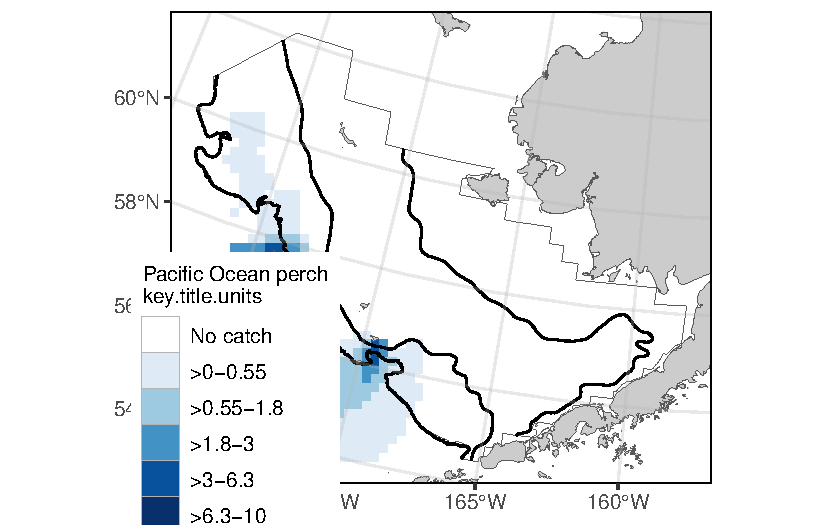
\includegraphics{content/akfin-oracle-sql-r_files/figure-pdf/test-6-fig-1.pdf}

}

\caption{Ex. 6: EBS Pacific Ocean perch CPUE and
\href{https://github.com/afsc-gap-products/akgfmaps}{\texttt{akgfmaps}}
map.}

\end{figure}

\part{Public Data (FOSS)}

This data contains all of the catch, environmental, and haul data from
the fisheries-independent Groundfish and Shellfish Assessment Program
surveys in the Bering Sea, Aleutian Islands, and Gulf of Alaska. This
data is sought after by the general public, private entities, and NOAA
partners alike, including tribal organizations, K-12 classrooms,
academic institutions, for-profit groups, and non-profit groups. This
data is compiled and approved once a year after each summer survey
season and is available for open access.

\part{Collaborators and data users}

Below are a few packages and products currently using this data. If you
have developed a product, performed an analysis, or exhibited this data
in any way, reach out so we can showcase your hard work.

\begin{itemize}
\item
  \textbf{\href{https://apps-st.fisheries.noaa.gov/dismap}{NOAA
  Fisheries Distribution Mapping and Analysis Portal}};
  \emph{\href{https://www.fisheries.noaa.gov/contact/office-science-and-technology}{NOAA
  Fisheries Office of Science and Technology}}
\item
  \textbf{\href{https://pyafscgap.org/}{Pull data with python} and
  explore the
  \href{https://app.pyafscgap.org/\textquotesingle{}}{in-browser
  visualization tool}. Reference their
  \href{https://mybinder.org/v2/gh/SchmidtDSE/afscgap/main?urlpath=/tree/index.ipynb}{example
  Python notebook}}; \emph{\href{https://dse.berkeley.edu/}{The Eric and
  Wendy Schmidt Center for Data Science and the Environment at UC
  Berkeley}, including sam.pottinger@berkeley.edu,
  ccmartinez@berkeley.edu, gzarpellon@berkeley.edu, and
  kkoy@berkeley.edu.}
\end{itemize}

\hypertarget{cite-this-data-3}{%
\section*{Cite this data}\label{cite-this-data-3}}
\addcontentsline{toc}{section}{Cite this data}

\markright{Cite this data}

Use the below
\href{https://github.com/afsc-gap-products/gap_products/blob/main/code/CITATION_FOSSAFSCData.bib}{bibtext
citations}, as cited in our group's
\href{https://github.com/afsc-gap-products/citations/blob/main/cite/bibliography.bib}{citation
repository} for citing the data created and maintained in this repo
(NOAA Fisheries Alaska Fisheries Science Center, 2023). Add ``note =
\{Accessed: mm/dd/yyyy\}'' to append the day this data was accessed.

\begin{verbatim}
@misc{FOSSAFSCData,
  author = {{NOAA Fisheries Alaska Fisheries Science Center}},
  year = {2023}, 
  title = {Fisheries One Stop Shop Public Data: RACE Division Bottom Trawl Survey Data Query},
  howpublished = {https://www.fisheries.noaa.gov/foss},
  publisher = {{U.S. Dep. Commer.}},
  copyright = {Public Domain} 
}
\end{verbatim}

\hypertarget{data-description-4}{%
\chapter{Data description}\label{data-description-4}}

The Resource Assessment and Conservation Engineering Division (RACE)
Groundfish Assessment Program (GAP) of the Alaska Fisheries Science
Center (AFSC) conducts fisheries-independent bottom trawl surveys to
monitor the condition of the demersal fish and crab stocks of Alaska.
These data are developed to describe the temporal distribution and
abundance of commercially and ecologically important groundfish species,
examine the changes in the species composition of the fauna over time
and space, and describe the physical environment of the groundfish
habitat.

There are no legal restrictions on access to the data. They reside in
the public domain and can be freely distributed. Users must read and
fully comprehend the metadata prior to use. Data should not be used
beyond the limits of the source scale. Acknowledgement of NOAA, as the
source from which these data were obtained, in any publications and/or
other representations of these data, is suggested. These data are
compiled and approved annually after each summer survey season. The data
from previous years are unlikely to change substantially once published.

These data are zero-filled (presence and absence) observations from
surveys conducted on fishing vessels. These surveys monitor trends in
distribution and abundance of groundfish, crab, and bottom-dwelling
species in Alaska's marine ecosystems. These data include estimates of
catch-per-unit-effort (CPUE) for all identified species for index
stations. Some survey data are excluded, such as non-standard stations,
surveys completed in earlier years using different/non-standard gear,
and special tows and non-standard data collections.

Though not included in the public data, these surveys also collect
oceanographic and environmental data, and biological data such as
length, weight, stomach contents (to learn more about diet), otoliths
(fish ear bones to learn about age), and tissue samples for genetic
analysis, all of which can be shared upon special request. Also not
included in the public data are estimated biomass (average total weight
of all fish and crabs sampled) of crabs and groundfish that support the
creation of annual stock assessments.

\hypertarget{data-tables-1}{%
\section{Data tables}\label{data-tables-1}}

\hypertarget{na-1}{%
\subsection{NA}\label{na-1}}

{[}There is currently no description for this table.{]}

Number of rows: 42S02 942 {[}Oracle{]}{[}ODBC{]}{[}Ora{]}ORA-00942:
table or view does not exist

Number of columns:

\begin{tabular}{l}
\hline
x\\
\hline
42S02 942 [Oracle][ODBC][Ora]ORA-00942: table or view does not exist\\
\hline
[RODBC] ERROR: Could not SQLExecDirect 'SELECT *
    FROM NA
    FETCH FIRST 3 ROWS ONLY;'\\
\hline
\end{tabular}

\hypertarget{section-306}{%
\subsection{}\label{section-306}}

Number of rows: 42S02 903 {[}Oracle{]}{[}ODBC{]}{[}Ora{]}ORA-00903:
invalid table name

Number of columns:

\begin{tabular}{l}
\hline
x\\
\hline
HY000 933 [Oracle][ODBC][Ora]ORA-00933: SQL command not properly ended\\
\hline
[RODBC] ERROR: Could not SQLExecDirect 'SELECT *
    FROM 
    FETCH FIRST 3 ROWS ONLY;'\\
\hline
\end{tabular}

, \#\#\# NA

{[}There is currently no description for this table.{]}

Number of rows: {[}RODBC{]} ERROR: Could not SQLExecDirect 'SELECT
COUNT(*) FROM NA;'

Number of columns:

\begin{tabular}{l}
\hline
x\\
\hline
42S02 942 [Oracle][ODBC][Ora]ORA-00942: table or view does not exist\\
\hline
[RODBC] ERROR: Could not SQLExecDirect 'SELECT *
    FROM NA
    FETCH FIRST 3 ROWS ONLY;'\\
\hline
\end{tabular}

\hypertarget{section-307}{%
\subsection{}\label{section-307}}

Number of rows: {[}RODBC{]} ERROR: Could not SQLExecDirect 'SELECT
COUNT(*) FROM ;'

Number of columns:

\begin{tabular}{l}
\hline
x\\
\hline
HY000 933 [Oracle][ODBC][Ora]ORA-00933: SQL command not properly ended\\
\hline
[RODBC] ERROR: Could not SQLExecDirect 'SELECT *
    FROM 
    FETCH FIRST 3 ROWS ONLY;'\\
\hline
\end{tabular}

, \#\#\# NA

{[}There is currently no description for this table.{]}

Number of rows: 42S02 942 {[}Oracle{]}{[}ODBC{]}{[}Ora{]}ORA-00942:
table or view does not exist

Number of columns:

\begin{tabular}{l}
\hline
x\\
\hline
42S02 942 [Oracle][ODBC][Ora]ORA-00942: table or view does not exist\\
\hline
[RODBC] ERROR: Could not SQLExecDirect 'SELECT *
    FROM NA
    FETCH FIRST 3 ROWS ONLY;'\\
\hline
\end{tabular}

\hypertarget{section-308}{%
\subsection{}\label{section-308}}

Number of rows: 42S02 903 {[}Oracle{]}{[}ODBC{]}{[}Ora{]}ORA-00903:
invalid table name

Number of columns:

\begin{tabular}{l}
\hline
x\\
\hline
HY000 933 [Oracle][ODBC][Ora]ORA-00933: SQL command not properly ended\\
\hline
[RODBC] ERROR: Could not SQLExecDirect 'SELECT *
    FROM 
    FETCH FIRST 3 ROWS ONLY;'\\
\hline
\end{tabular}

, \#\#\# NA

{[}There is currently no description for this table.{]}

Number of rows: {[}RODBC{]} ERROR: Could not SQLExecDirect 'SELECT
COUNT(*) FROM NA;'

Number of columns:

\begin{tabular}{l}
\hline
x\\
\hline
42S02 942 [Oracle][ODBC][Ora]ORA-00942: table or view does not exist\\
\hline
[RODBC] ERROR: Could not SQLExecDirect 'SELECT *
    FROM NA
    FETCH FIRST 3 ROWS ONLY;'\\
\hline
\end{tabular}

\hypertarget{section-309}{%
\subsection{}\label{section-309}}

Number of rows: {[}RODBC{]} ERROR: Could not SQLExecDirect 'SELECT
COUNT(*) FROM ;'

Number of columns:

\begin{tabular}{l}
\hline
x\\
\hline
HY000 933 [Oracle][ODBC][Ora]ORA-00933: SQL command not properly ended\\
\hline
[RODBC] ERROR: Could not SQLExecDirect 'SELECT *
    FROM 
    FETCH FIRST 3 ROWS ONLY;'\\
\hline
\end{tabular}

, \#\#\# NA

{[}There is currently no description for this table.{]}

Number of rows: 42S02 942 {[}Oracle{]}{[}ODBC{]}{[}Ora{]}ORA-00942:
table or view does not exist

Number of columns:

\begin{tabular}{l}
\hline
x\\
\hline
42S02 942 [Oracle][ODBC][Ora]ORA-00942: table or view does not exist\\
\hline
[RODBC] ERROR: Could not SQLExecDirect 'SELECT *
    FROM NA
    FETCH FIRST 3 ROWS ONLY;'\\
\hline
\end{tabular}

\hypertarget{section-310}{%
\subsection{}\label{section-310}}

Number of rows: 42S02 903 {[}Oracle{]}{[}ODBC{]}{[}Ora{]}ORA-00903:
invalid table name

Number of columns:

\begin{tabular}{l}
\hline
x\\
\hline
HY000 933 [Oracle][ODBC][Ora]ORA-00933: SQL command not properly ended\\
\hline
[RODBC] ERROR: Could not SQLExecDirect 'SELECT *
    FROM 
    FETCH FIRST 3 ROWS ONLY;'\\
\hline
\end{tabular}

, \#\#\# NA

{[}There is currently no description for this table.{]}

Number of rows: {[}RODBC{]} ERROR: Could not SQLExecDirect 'SELECT
COUNT(*) FROM NA;'

Number of columns:

\begin{tabular}{l}
\hline
x\\
\hline
42S02 942 [Oracle][ODBC][Ora]ORA-00942: table or view does not exist\\
\hline
[RODBC] ERROR: Could not SQLExecDirect 'SELECT *
    FROM NA
    FETCH FIRST 3 ROWS ONLY;'\\
\hline
\end{tabular}

\hypertarget{section-311}{%
\subsection{}\label{section-311}}

Number of rows: {[}RODBC{]} ERROR: Could not SQLExecDirect 'SELECT
COUNT(*) FROM ;'

Number of columns:

\begin{tabular}{l}
\hline
x\\
\hline
HY000 933 [Oracle][ODBC][Ora]ORA-00933: SQL command not properly ended\\
\hline
[RODBC] ERROR: Could not SQLExecDirect 'SELECT *
    FROM 
    FETCH FIRST 3 ROWS ONLY;'\\
\hline
\end{tabular}

, \#\#\# NA

{[}There is currently no description for this table.{]}

Number of rows: 42S02 942 {[}Oracle{]}{[}ODBC{]}{[}Ora{]}ORA-00942:
table or view does not exist

Number of columns:

\begin{tabular}{l}
\hline
x\\
\hline
42S02 942 [Oracle][ODBC][Ora]ORA-00942: table or view does not exist\\
\hline
[RODBC] ERROR: Could not SQLExecDirect 'SELECT *
    FROM NA
    FETCH FIRST 3 ROWS ONLY;'\\
\hline
\end{tabular}

\hypertarget{section-312}{%
\subsection{}\label{section-312}}

Number of rows: 42S02 903 {[}Oracle{]}{[}ODBC{]}{[}Ora{]}ORA-00903:
invalid table name

Number of columns:

\begin{tabular}{l}
\hline
x\\
\hline
HY000 933 [Oracle][ODBC][Ora]ORA-00933: SQL command not properly ended\\
\hline
[RODBC] ERROR: Could not SQLExecDirect 'SELECT *
    FROM 
    FETCH FIRST 3 ROWS ONLY;'\\
\hline
\end{tabular}

, \#\#\# NA

{[}There is currently no description for this table.{]}

Number of rows: {[}RODBC{]} ERROR: Could not SQLExecDirect 'SELECT
COUNT(*) FROM NA;'

Number of columns:

\begin{tabular}{l}
\hline
x\\
\hline
42S02 942 [Oracle][ODBC][Ora]ORA-00942: table or view does not exist\\
\hline
[RODBC] ERROR: Could not SQLExecDirect 'SELECT *
    FROM NA
    FETCH FIRST 3 ROWS ONLY;'\\
\hline
\end{tabular}

\hypertarget{section-313}{%
\subsection{}\label{section-313}}

Number of rows: {[}RODBC{]} ERROR: Could not SQLExecDirect 'SELECT
COUNT(*) FROM ;'

Number of columns:

\begin{tabular}{l}
\hline
x\\
\hline
HY000 933 [Oracle][ODBC][Ora]ORA-00933: SQL command not properly ended\\
\hline
[RODBC] ERROR: Could not SQLExecDirect 'SELECT *
    FROM 
    FETCH FIRST 3 ROWS ONLY;'\\
\hline
\end{tabular}

, \#\#\# NA

{[}There is currently no description for this table.{]}

Number of rows: 42S02 942 {[}Oracle{]}{[}ODBC{]}{[}Ora{]}ORA-00942:
table or view does not exist

Number of columns:

\begin{tabular}{l}
\hline
x\\
\hline
42S02 942 [Oracle][ODBC][Ora]ORA-00942: table or view does not exist\\
\hline
[RODBC] ERROR: Could not SQLExecDirect 'SELECT *
    FROM NA
    FETCH FIRST 3 ROWS ONLY;'\\
\hline
\end{tabular}

\hypertarget{section-314}{%
\subsection{}\label{section-314}}

Number of rows: 42S02 903 {[}Oracle{]}{[}ODBC{]}{[}Ora{]}ORA-00903:
invalid table name

Number of columns:

\begin{tabular}{l}
\hline
x\\
\hline
HY000 933 [Oracle][ODBC][Ora]ORA-00933: SQL command not properly ended\\
\hline
[RODBC] ERROR: Could not SQLExecDirect 'SELECT *
    FROM 
    FETCH FIRST 3 ROWS ONLY;'\\
\hline
\end{tabular}

, \#\#\# NA

{[}There is currently no description for this table.{]}

Number of rows: {[}RODBC{]} ERROR: Could not SQLExecDirect 'SELECT
COUNT(*) FROM NA;'

Number of columns:

\begin{tabular}{l}
\hline
x\\
\hline
42S02 942 [Oracle][ODBC][Ora]ORA-00942: table or view does not exist\\
\hline
[RODBC] ERROR: Could not SQLExecDirect 'SELECT *
    FROM NA
    FETCH FIRST 3 ROWS ONLY;'\\
\hline
\end{tabular}

\hypertarget{section-315}{%
\subsection{}\label{section-315}}

Number of rows: {[}RODBC{]} ERROR: Could not SQLExecDirect 'SELECT
COUNT(*) FROM ;'

Number of columns:

\begin{tabular}{l}
\hline
x\\
\hline
HY000 933 [Oracle][ODBC][Ora]ORA-00933: SQL command not properly ended\\
\hline
[RODBC] ERROR: Could not SQLExecDirect 'SELECT *
    FROM 
    FETCH FIRST 3 ROWS ONLY;'\\
\hline
\end{tabular}

, \#\#\# NA

{[}There is currently no description for this table.{]}

Number of rows: 42S02 942 {[}Oracle{]}{[}ODBC{]}{[}Ora{]}ORA-00942:
table or view does not exist

Number of columns:

\begin{tabular}{l}
\hline
x\\
\hline
42S02 942 [Oracle][ODBC][Ora]ORA-00942: table or view does not exist\\
\hline
[RODBC] ERROR: Could not SQLExecDirect 'SELECT *
    FROM NA
    FETCH FIRST 3 ROWS ONLY;'\\
\hline
\end{tabular}

\hypertarget{section-316}{%
\subsection{}\label{section-316}}

Number of rows: 42S02 903 {[}Oracle{]}{[}ODBC{]}{[}Ora{]}ORA-00903:
invalid table name

Number of columns:

\begin{tabular}{l}
\hline
x\\
\hline
HY000 933 [Oracle][ODBC][Ora]ORA-00933: SQL command not properly ended\\
\hline
[RODBC] ERROR: Could not SQLExecDirect 'SELECT *
    FROM 
    FETCH FIRST 3 ROWS ONLY;'\\
\hline
\end{tabular}

, \#\#\# NA

{[}There is currently no description for this table.{]}

Number of rows: {[}RODBC{]} ERROR: Could not SQLExecDirect 'SELECT
COUNT(*) FROM NA;'

Number of columns:

\begin{tabular}{l}
\hline
x\\
\hline
42S02 942 [Oracle][ODBC][Ora]ORA-00942: table or view does not exist\\
\hline
[RODBC] ERROR: Could not SQLExecDirect 'SELECT *
    FROM NA
    FETCH FIRST 3 ROWS ONLY;'\\
\hline
\end{tabular}

\hypertarget{section-317}{%
\subsection{}\label{section-317}}

Number of rows: {[}RODBC{]} ERROR: Could not SQLExecDirect 'SELECT
COUNT(*) FROM ;'

Number of columns:

\begin{tabular}{l}
\hline
x\\
\hline
HY000 933 [Oracle][ODBC][Ora]ORA-00933: SQL command not properly ended\\
\hline
[RODBC] ERROR: Could not SQLExecDirect 'SELECT *
    FROM 
    FETCH FIRST 3 ROWS ONLY;'\\
\hline
\end{tabular}

, \#\#\# NA

{[}There is currently no description for this table.{]}

Number of rows: 42S02 942 {[}Oracle{]}{[}ODBC{]}{[}Ora{]}ORA-00942:
table or view does not exist

Number of columns:

\begin{tabular}{l}
\hline
x\\
\hline
42S02 942 [Oracle][ODBC][Ora]ORA-00942: table or view does not exist\\
\hline
[RODBC] ERROR: Could not SQLExecDirect 'SELECT *
    FROM NA
    FETCH FIRST 3 ROWS ONLY;'\\
\hline
\end{tabular}

\hypertarget{section-318}{%
\subsection{}\label{section-318}}

Number of rows: 42S02 903 {[}Oracle{]}{[}ODBC{]}{[}Ora{]}ORA-00903:
invalid table name

Number of columns:

\begin{tabular}{l}
\hline
x\\
\hline
HY000 933 [Oracle][ODBC][Ora]ORA-00933: SQL command not properly ended\\
\hline
[RODBC] ERROR: Could not SQLExecDirect 'SELECT *
    FROM 
    FETCH FIRST 3 ROWS ONLY;'\\
\hline
\end{tabular}

, \#\#\# NA

{[}There is currently no description for this table.{]}

Number of rows: {[}RODBC{]} ERROR: Could not SQLExecDirect 'SELECT
COUNT(*) FROM NA;'

Number of columns:

\begin{tabular}{l}
\hline
x\\
\hline
42S02 942 [Oracle][ODBC][Ora]ORA-00942: table or view does not exist\\
\hline
[RODBC] ERROR: Could not SQLExecDirect 'SELECT *
    FROM NA
    FETCH FIRST 3 ROWS ONLY;'\\
\hline
\end{tabular}

\hypertarget{section-319}{%
\subsection{}\label{section-319}}

Number of rows: {[}RODBC{]} ERROR: Could not SQLExecDirect 'SELECT
COUNT(*) FROM ;'

Number of columns:

\begin{tabular}{l}
\hline
x\\
\hline
HY000 933 [Oracle][ODBC][Ora]ORA-00933: SQL command not properly ended\\
\hline
[RODBC] ERROR: Could not SQLExecDirect 'SELECT *
    FROM 
    FETCH FIRST 3 ROWS ONLY;'\\
\hline
\end{tabular}

, \#\#\# NA

{[}There is currently no description for this table.{]}

Number of rows: 42S02 942 {[}Oracle{]}{[}ODBC{]}{[}Ora{]}ORA-00942:
table or view does not exist

Number of columns:

\begin{tabular}{l}
\hline
x\\
\hline
42S02 942 [Oracle][ODBC][Ora]ORA-00942: table or view does not exist\\
\hline
[RODBC] ERROR: Could not SQLExecDirect 'SELECT *
    FROM NA
    FETCH FIRST 3 ROWS ONLY;'\\
\hline
\end{tabular}

\hypertarget{section-320}{%
\subsection{}\label{section-320}}

Number of rows: 42S02 903 {[}Oracle{]}{[}ODBC{]}{[}Ora{]}ORA-00903:
invalid table name

Number of columns:

\begin{tabular}{l}
\hline
x\\
\hline
HY000 933 [Oracle][ODBC][Ora]ORA-00933: SQL command not properly ended\\
\hline
[RODBC] ERROR: Could not SQLExecDirect 'SELECT *
    FROM 
    FETCH FIRST 3 ROWS ONLY;'\\
\hline
\end{tabular}

, \#\#\# NA

{[}There is currently no description for this table.{]}

Number of rows: {[}RODBC{]} ERROR: Could not SQLExecDirect 'SELECT
COUNT(*) FROM NA;'

Number of columns:

\begin{tabular}{l}
\hline
x\\
\hline
42S02 942 [Oracle][ODBC][Ora]ORA-00942: table or view does not exist\\
\hline
[RODBC] ERROR: Could not SQLExecDirect 'SELECT *
    FROM NA
    FETCH FIRST 3 ROWS ONLY;'\\
\hline
\end{tabular}

\hypertarget{section-321}{%
\subsection{}\label{section-321}}

Number of rows: {[}RODBC{]} ERROR: Could not SQLExecDirect 'SELECT
COUNT(*) FROM ;'

Number of columns:

\begin{tabular}{l}
\hline
x\\
\hline
HY000 933 [Oracle][ODBC][Ora]ORA-00933: SQL command not properly ended\\
\hline
[RODBC] ERROR: Could not SQLExecDirect 'SELECT *
    FROM 
    FETCH FIRST 3 ROWS ONLY;'\\
\hline
\end{tabular}

, \#\#\# NA

{[}There is currently no description for this table.{]}

Number of rows: 42S02 942 {[}Oracle{]}{[}ODBC{]}{[}Ora{]}ORA-00942:
table or view does not exist

Number of columns:

\begin{tabular}{l}
\hline
x\\
\hline
42S02 942 [Oracle][ODBC][Ora]ORA-00942: table or view does not exist\\
\hline
[RODBC] ERROR: Could not SQLExecDirect 'SELECT *
    FROM NA
    FETCH FIRST 3 ROWS ONLY;'\\
\hline
\end{tabular}

\hypertarget{section-322}{%
\subsection{}\label{section-322}}

Number of rows: 42S02 903 {[}Oracle{]}{[}ODBC{]}{[}Ora{]}ORA-00903:
invalid table name

Number of columns:

\begin{tabular}{l}
\hline
x\\
\hline
HY000 933 [Oracle][ODBC][Ora]ORA-00933: SQL command not properly ended\\
\hline
[RODBC] ERROR: Could not SQLExecDirect 'SELECT *
    FROM 
    FETCH FIRST 3 ROWS ONLY;'\\
\hline
\end{tabular}

, \#\#\# NA

{[}There is currently no description for this table.{]}

Number of rows: {[}RODBC{]} ERROR: Could not SQLExecDirect 'SELECT
COUNT(*) FROM NA;'

Number of columns:

\begin{tabular}{l}
\hline
x\\
\hline
42S02 942 [Oracle][ODBC][Ora]ORA-00942: table or view does not exist\\
\hline
[RODBC] ERROR: Could not SQLExecDirect 'SELECT *
    FROM NA
    FETCH FIRST 3 ROWS ONLY;'\\
\hline
\end{tabular}

\hypertarget{section-323}{%
\subsection{}\label{section-323}}

Number of rows: {[}RODBC{]} ERROR: Could not SQLExecDirect 'SELECT
COUNT(*) FROM ;'

Number of columns:

\begin{tabular}{l}
\hline
x\\
\hline
HY000 933 [Oracle][ODBC][Ora]ORA-00933: SQL command not properly ended\\
\hline
[RODBC] ERROR: Could not SQLExecDirect 'SELECT *
    FROM 
    FETCH FIRST 3 ROWS ONLY;'\\
\hline
\end{tabular}

, \#\#\# NA

{[}There is currently no description for this table.{]}

Number of rows: 42S02 942 {[}Oracle{]}{[}ODBC{]}{[}Ora{]}ORA-00942:
table or view does not exist

Number of columns:

\begin{tabular}{l}
\hline
x\\
\hline
42S02 942 [Oracle][ODBC][Ora]ORA-00942: table or view does not exist\\
\hline
[RODBC] ERROR: Could not SQLExecDirect 'SELECT *
    FROM NA
    FETCH FIRST 3 ROWS ONLY;'\\
\hline
\end{tabular}

\hypertarget{section-324}{%
\subsection{}\label{section-324}}

Number of rows: 42S02 903 {[}Oracle{]}{[}ODBC{]}{[}Ora{]}ORA-00903:
invalid table name

Number of columns:

\begin{tabular}{l}
\hline
x\\
\hline
HY000 933 [Oracle][ODBC][Ora]ORA-00933: SQL command not properly ended\\
\hline
[RODBC] ERROR: Could not SQLExecDirect 'SELECT *
    FROM 
    FETCH FIRST 3 ROWS ONLY;'\\
\hline
\end{tabular}

, \#\#\# NA

{[}There is currently no description for this table.{]}

Number of rows: {[}RODBC{]} ERROR: Could not SQLExecDirect 'SELECT
COUNT(*) FROM NA;'

Number of columns:

\begin{tabular}{l}
\hline
x\\
\hline
42S02 942 [Oracle][ODBC][Ora]ORA-00942: table or view does not exist\\
\hline
[RODBC] ERROR: Could not SQLExecDirect 'SELECT *
    FROM NA
    FETCH FIRST 3 ROWS ONLY;'\\
\hline
\end{tabular}

\hypertarget{section-325}{%
\subsection{}\label{section-325}}

Number of rows: {[}RODBC{]} ERROR: Could not SQLExecDirect 'SELECT
COUNT(*) FROM ;'

Number of columns:

\begin{tabular}{l}
\hline
x\\
\hline
HY000 933 [Oracle][ODBC][Ora]ORA-00933: SQL command not properly ended\\
\hline
[RODBC] ERROR: Could not SQLExecDirect 'SELECT *
    FROM 
    FETCH FIRST 3 ROWS ONLY;'\\
\hline
\end{tabular}

, \#\#\# NA

{[}There is currently no description for this table.{]}

Number of rows: 42S02 942 {[}Oracle{]}{[}ODBC{]}{[}Ora{]}ORA-00942:
table or view does not exist

Number of columns:

\begin{tabular}{l}
\hline
x\\
\hline
42S02 942 [Oracle][ODBC][Ora]ORA-00942: table or view does not exist\\
\hline
[RODBC] ERROR: Could not SQLExecDirect 'SELECT *
    FROM NA
    FETCH FIRST 3 ROWS ONLY;'\\
\hline
\end{tabular}

\hypertarget{section-326}{%
\subsection{}\label{section-326}}

Number of rows: 42S02 903 {[}Oracle{]}{[}ODBC{]}{[}Ora{]}ORA-00903:
invalid table name

Number of columns:

\begin{tabular}{l}
\hline
x\\
\hline
HY000 933 [Oracle][ODBC][Ora]ORA-00933: SQL command not properly ended\\
\hline
[RODBC] ERROR: Could not SQLExecDirect 'SELECT *
    FROM 
    FETCH FIRST 3 ROWS ONLY;'\\
\hline
\end{tabular}

, \#\#\# NA

{[}There is currently no description for this table.{]}

Number of rows: {[}RODBC{]} ERROR: Could not SQLExecDirect 'SELECT
COUNT(*) FROM NA;'

Number of columns:

\begin{tabular}{l}
\hline
x\\
\hline
42S02 942 [Oracle][ODBC][Ora]ORA-00942: table or view does not exist\\
\hline
[RODBC] ERROR: Could not SQLExecDirect 'SELECT *
    FROM NA
    FETCH FIRST 3 ROWS ONLY;'\\
\hline
\end{tabular}

\hypertarget{section-327}{%
\subsection{}\label{section-327}}

Number of rows: {[}RODBC{]} ERROR: Could not SQLExecDirect 'SELECT
COUNT(*) FROM ;'

Number of columns:

\begin{tabular}{l}
\hline
x\\
\hline
HY000 933 [Oracle][ODBC][Ora]ORA-00933: SQL command not properly ended\\
\hline
[RODBC] ERROR: Could not SQLExecDirect 'SELECT *
    FROM 
    FETCH FIRST 3 ROWS ONLY;'\\
\hline
\end{tabular}

, \#\#\# NA

{[}There is currently no description for this table.{]}

Number of rows: 42S02 942 {[}Oracle{]}{[}ODBC{]}{[}Ora{]}ORA-00942:
table or view does not exist

Number of columns:

\begin{tabular}{l}
\hline
x\\
\hline
42S02 942 [Oracle][ODBC][Ora]ORA-00942: table or view does not exist\\
\hline
[RODBC] ERROR: Could not SQLExecDirect 'SELECT *
    FROM NA
    FETCH FIRST 3 ROWS ONLY;'\\
\hline
\end{tabular}

\hypertarget{section-328}{%
\subsection{}\label{section-328}}

Number of rows: 42S02 903 {[}Oracle{]}{[}ODBC{]}{[}Ora{]}ORA-00903:
invalid table name

Number of columns:

\begin{tabular}{l}
\hline
x\\
\hline
HY000 933 [Oracle][ODBC][Ora]ORA-00933: SQL command not properly ended\\
\hline
[RODBC] ERROR: Could not SQLExecDirect 'SELECT *
    FROM 
    FETCH FIRST 3 ROWS ONLY;'\\
\hline
\end{tabular}

, \#\#\# NA

{[}There is currently no description for this table.{]}

Number of rows: {[}RODBC{]} ERROR: Could not SQLExecDirect 'SELECT
COUNT(*) FROM NA;'

Number of columns:

\begin{tabular}{l}
\hline
x\\
\hline
42S02 942 [Oracle][ODBC][Ora]ORA-00942: table or view does not exist\\
\hline
[RODBC] ERROR: Could not SQLExecDirect 'SELECT *
    FROM NA
    FETCH FIRST 3 ROWS ONLY;'\\
\hline
\end{tabular}

\hypertarget{section-329}{%
\subsection{}\label{section-329}}

Number of rows: {[}RODBC{]} ERROR: Could not SQLExecDirect 'SELECT
COUNT(*) FROM ;'

Number of columns:

\begin{tabular}{l}
\hline
x\\
\hline
HY000 933 [Oracle][ODBC][Ora]ORA-00933: SQL command not properly ended\\
\hline
[RODBC] ERROR: Could not SQLExecDirect 'SELECT *
    FROM 
    FETCH FIRST 3 ROWS ONLY;'\\
\hline
\end{tabular}

, \#\#\# NA

{[}There is currently no description for this table.{]}

Number of rows: 42S02 942 {[}Oracle{]}{[}ODBC{]}{[}Ora{]}ORA-00942:
table or view does not exist

Number of columns:

\begin{tabular}{l}
\hline
x\\
\hline
42S02 942 [Oracle][ODBC][Ora]ORA-00942: table or view does not exist\\
\hline
[RODBC] ERROR: Could not SQLExecDirect 'SELECT *
    FROM NA
    FETCH FIRST 3 ROWS ONLY;'\\
\hline
\end{tabular}

\hypertarget{section-330}{%
\subsection{}\label{section-330}}

Number of rows: 42S02 903 {[}Oracle{]}{[}ODBC{]}{[}Ora{]}ORA-00903:
invalid table name

Number of columns:

\begin{tabular}{l}
\hline
x\\
\hline
HY000 933 [Oracle][ODBC][Ora]ORA-00933: SQL command not properly ended\\
\hline
[RODBC] ERROR: Could not SQLExecDirect 'SELECT *
    FROM 
    FETCH FIRST 3 ROWS ONLY;'\\
\hline
\end{tabular}

, \#\#\# NA

{[}There is currently no description for this table.{]}

Number of rows: {[}RODBC{]} ERROR: Could not SQLExecDirect 'SELECT
COUNT(*) FROM NA;'

Number of columns:

\begin{tabular}{l}
\hline
x\\
\hline
42S02 942 [Oracle][ODBC][Ora]ORA-00942: table or view does not exist\\
\hline
[RODBC] ERROR: Could not SQLExecDirect 'SELECT *
    FROM NA
    FETCH FIRST 3 ROWS ONLY;'\\
\hline
\end{tabular}

\hypertarget{section-331}{%
\subsection{}\label{section-331}}

Number of rows: {[}RODBC{]} ERROR: Could not SQLExecDirect 'SELECT
COUNT(*) FROM ;'

Number of columns:

\begin{tabular}{l}
\hline
x\\
\hline
HY000 933 [Oracle][ODBC][Ora]ORA-00933: SQL command not properly ended\\
\hline
[RODBC] ERROR: Could not SQLExecDirect 'SELECT *
    FROM 
    FETCH FIRST 3 ROWS ONLY;'\\
\hline
\end{tabular}

, \#\#\# NA

{[}There is currently no description for this table.{]}

Number of rows: 42S02 942 {[}Oracle{]}{[}ODBC{]}{[}Ora{]}ORA-00942:
table or view does not exist

Number of columns:

\begin{tabular}{l}
\hline
x\\
\hline
42S02 942 [Oracle][ODBC][Ora]ORA-00942: table or view does not exist\\
\hline
[RODBC] ERROR: Could not SQLExecDirect 'SELECT *
    FROM NA
    FETCH FIRST 3 ROWS ONLY;'\\
\hline
\end{tabular}

\hypertarget{section-332}{%
\subsection{}\label{section-332}}

Number of rows: 42S02 903 {[}Oracle{]}{[}ODBC{]}{[}Ora{]}ORA-00903:
invalid table name

Number of columns:

\begin{tabular}{l}
\hline
x\\
\hline
HY000 933 [Oracle][ODBC][Ora]ORA-00933: SQL command not properly ended\\
\hline
[RODBC] ERROR: Could not SQLExecDirect 'SELECT *
    FROM 
    FETCH FIRST 3 ROWS ONLY;'\\
\hline
\end{tabular}

, \#\#\# NA

{[}There is currently no description for this table.{]}

Number of rows: {[}RODBC{]} ERROR: Could not SQLExecDirect 'SELECT
COUNT(*) FROM NA;'

Number of columns:

\begin{tabular}{l}
\hline
x\\
\hline
42S02 942 [Oracle][ODBC][Ora]ORA-00942: table or view does not exist\\
\hline
[RODBC] ERROR: Could not SQLExecDirect 'SELECT *
    FROM NA
    FETCH FIRST 3 ROWS ONLY;'\\
\hline
\end{tabular}

\hypertarget{section-333}{%
\subsection{}\label{section-333}}

Number of rows: {[}RODBC{]} ERROR: Could not SQLExecDirect 'SELECT
COUNT(*) FROM ;'

Number of columns:

\begin{tabular}{l}
\hline
x\\
\hline
HY000 933 [Oracle][ODBC][Ora]ORA-00933: SQL command not properly ended\\
\hline
[RODBC] ERROR: Could not SQLExecDirect 'SELECT *
    FROM 
    FETCH FIRST 3 ROWS ONLY;'\\
\hline
\end{tabular}

, \#\#\# NA

{[}There is currently no description for this table.{]}

Number of rows: 42S02 942 {[}Oracle{]}{[}ODBC{]}{[}Ora{]}ORA-00942:
table or view does not exist

Number of columns:

\begin{tabular}{l}
\hline
x\\
\hline
42S02 942 [Oracle][ODBC][Ora]ORA-00942: table or view does not exist\\
\hline
[RODBC] ERROR: Could not SQLExecDirect 'SELECT *
    FROM NA
    FETCH FIRST 3 ROWS ONLY;'\\
\hline
\end{tabular}

\hypertarget{section-334}{%
\subsection{}\label{section-334}}

Number of rows: 42S02 903 {[}Oracle{]}{[}ODBC{]}{[}Ora{]}ORA-00903:
invalid table name

Number of columns:

\begin{tabular}{l}
\hline
x\\
\hline
HY000 933 [Oracle][ODBC][Ora]ORA-00933: SQL command not properly ended\\
\hline
[RODBC] ERROR: Could not SQLExecDirect 'SELECT *
    FROM 
    FETCH FIRST 3 ROWS ONLY;'\\
\hline
\end{tabular}

, \#\#\# NA

{[}There is currently no description for this table.{]}

Number of rows: {[}RODBC{]} ERROR: Could not SQLExecDirect 'SELECT
COUNT(*) FROM NA;'

Number of columns:

\begin{tabular}{l}
\hline
x\\
\hline
42S02 942 [Oracle][ODBC][Ora]ORA-00942: table or view does not exist\\
\hline
[RODBC] ERROR: Could not SQLExecDirect 'SELECT *
    FROM NA
    FETCH FIRST 3 ROWS ONLY;'\\
\hline
\end{tabular}

\hypertarget{section-335}{%
\subsection{}\label{section-335}}

Number of rows: {[}RODBC{]} ERROR: Could not SQLExecDirect 'SELECT
COUNT(*) FROM ;'

Number of columns:

\begin{tabular}{l}
\hline
x\\
\hline
HY000 933 [Oracle][ODBC][Ora]ORA-00933: SQL command not properly ended\\
\hline
[RODBC] ERROR: Could not SQLExecDirect 'SELECT *
    FROM 
    FETCH FIRST 3 ROWS ONLY;'\\
\hline
\end{tabular}

, \#\#\# NA

{[}There is currently no description for this table.{]}

Number of rows: 42S02 942 {[}Oracle{]}{[}ODBC{]}{[}Ora{]}ORA-00942:
table or view does not exist

Number of columns:

\begin{tabular}{l}
\hline
x\\
\hline
42S02 942 [Oracle][ODBC][Ora]ORA-00942: table or view does not exist\\
\hline
[RODBC] ERROR: Could not SQLExecDirect 'SELECT *
    FROM NA
    FETCH FIRST 3 ROWS ONLY;'\\
\hline
\end{tabular}

\hypertarget{section-336}{%
\subsection{}\label{section-336}}

Number of rows: 42S02 903 {[}Oracle{]}{[}ODBC{]}{[}Ora{]}ORA-00903:
invalid table name

Number of columns:

\begin{tabular}{l}
\hline
x\\
\hline
HY000 933 [Oracle][ODBC][Ora]ORA-00933: SQL command not properly ended\\
\hline
[RODBC] ERROR: Could not SQLExecDirect 'SELECT *
    FROM 
    FETCH FIRST 3 ROWS ONLY;'\\
\hline
\end{tabular}

, \#\#\# NA

{[}There is currently no description for this table.{]}

Number of rows: {[}RODBC{]} ERROR: Could not SQLExecDirect 'SELECT
COUNT(*) FROM NA;'

Number of columns:

\begin{tabular}{l}
\hline
x\\
\hline
42S02 942 [Oracle][ODBC][Ora]ORA-00942: table or view does not exist\\
\hline
[RODBC] ERROR: Could not SQLExecDirect 'SELECT *
    FROM NA
    FETCH FIRST 3 ROWS ONLY;'\\
\hline
\end{tabular}

\hypertarget{section-337}{%
\subsection{}\label{section-337}}

Number of rows: {[}RODBC{]} ERROR: Could not SQLExecDirect 'SELECT
COUNT(*) FROM ;'

Number of columns:

\begin{tabular}{l}
\hline
x\\
\hline
HY000 933 [Oracle][ODBC][Ora]ORA-00933: SQL command not properly ended\\
\hline
[RODBC] ERROR: Could not SQLExecDirect 'SELECT *
    FROM 
    FETCH FIRST 3 ROWS ONLY;'\\
\hline
\end{tabular}

, \#\#\# NA

{[}There is currently no description for this table.{]}

Number of rows: 42S02 942 {[}Oracle{]}{[}ODBC{]}{[}Ora{]}ORA-00942:
table or view does not exist

Number of columns:

\begin{tabular}{l}
\hline
x\\
\hline
42S02 942 [Oracle][ODBC][Ora]ORA-00942: table or view does not exist\\
\hline
[RODBC] ERROR: Could not SQLExecDirect 'SELECT *
    FROM NA
    FETCH FIRST 3 ROWS ONLY;'\\
\hline
\end{tabular}

\hypertarget{section-338}{%
\subsection{}\label{section-338}}

Number of rows: 42S02 903 {[}Oracle{]}{[}ODBC{]}{[}Ora{]}ORA-00903:
invalid table name

Number of columns:

\begin{tabular}{l}
\hline
x\\
\hline
HY000 933 [Oracle][ODBC][Ora]ORA-00933: SQL command not properly ended\\
\hline
[RODBC] ERROR: Could not SQLExecDirect 'SELECT *
    FROM 
    FETCH FIRST 3 ROWS ONLY;'\\
\hline
\end{tabular}

, \#\#\# NA

{[}There is currently no description for this table.{]}

Number of rows: {[}RODBC{]} ERROR: Could not SQLExecDirect 'SELECT
COUNT(*) FROM NA;'

Number of columns:

\begin{tabular}{l}
\hline
x\\
\hline
42S02 942 [Oracle][ODBC][Ora]ORA-00942: table or view does not exist\\
\hline
[RODBC] ERROR: Could not SQLExecDirect 'SELECT *
    FROM NA
    FETCH FIRST 3 ROWS ONLY;'\\
\hline
\end{tabular}

\hypertarget{section-339}{%
\subsection{}\label{section-339}}

Number of rows: {[}RODBC{]} ERROR: Could not SQLExecDirect 'SELECT
COUNT(*) FROM ;'

Number of columns:

\begin{tabular}{l}
\hline
x\\
\hline
HY000 933 [Oracle][ODBC][Ora]ORA-00933: SQL command not properly ended\\
\hline
[RODBC] ERROR: Could not SQLExecDirect 'SELECT *
    FROM 
    FETCH FIRST 3 ROWS ONLY;'\\
\hline
\end{tabular}

, \#\#\# NA

{[}There is currently no description for this table.{]}

Number of rows: 42S02 942 {[}Oracle{]}{[}ODBC{]}{[}Ora{]}ORA-00942:
table or view does not exist

Number of columns:

\begin{tabular}{l}
\hline
x\\
\hline
42S02 942 [Oracle][ODBC][Ora]ORA-00942: table or view does not exist\\
\hline
[RODBC] ERROR: Could not SQLExecDirect 'SELECT *
    FROM NA
    FETCH FIRST 3 ROWS ONLY;'\\
\hline
\end{tabular}

\hypertarget{section-340}{%
\subsection{}\label{section-340}}

Number of rows: 42S02 903 {[}Oracle{]}{[}ODBC{]}{[}Ora{]}ORA-00903:
invalid table name

Number of columns:

\begin{tabular}{l}
\hline
x\\
\hline
HY000 933 [Oracle][ODBC][Ora]ORA-00933: SQL command not properly ended\\
\hline
[RODBC] ERROR: Could not SQLExecDirect 'SELECT *
    FROM 
    FETCH FIRST 3 ROWS ONLY;'\\
\hline
\end{tabular}

, \#\#\# NA

{[}There is currently no description for this table.{]}

Number of rows: {[}RODBC{]} ERROR: Could not SQLExecDirect 'SELECT
COUNT(*) FROM NA;'

Number of columns:

\begin{tabular}{l}
\hline
x\\
\hline
42S02 942 [Oracle][ODBC][Ora]ORA-00942: table or view does not exist\\
\hline
[RODBC] ERROR: Could not SQLExecDirect 'SELECT *
    FROM NA
    FETCH FIRST 3 ROWS ONLY;'\\
\hline
\end{tabular}

\hypertarget{section-341}{%
\subsection{}\label{section-341}}

Number of rows: {[}RODBC{]} ERROR: Could not SQLExecDirect 'SELECT
COUNT(*) FROM ;'

Number of columns:

\begin{tabular}{l}
\hline
x\\
\hline
HY000 933 [Oracle][ODBC][Ora]ORA-00933: SQL command not properly ended\\
\hline
[RODBC] ERROR: Could not SQLExecDirect 'SELECT *
    FROM 
    FETCH FIRST 3 ROWS ONLY;'\\
\hline
\end{tabular}

, \#\#\# NA

{[}There is currently no description for this table.{]}

Number of rows: 42S02 942 {[}Oracle{]}{[}ODBC{]}{[}Ora{]}ORA-00942:
table or view does not exist

Number of columns:

\begin{tabular}{l}
\hline
x\\
\hline
42S02 942 [Oracle][ODBC][Ora]ORA-00942: table or view does not exist\\
\hline
[RODBC] ERROR: Could not SQLExecDirect 'SELECT *
    FROM NA
    FETCH FIRST 3 ROWS ONLY;'\\
\hline
\end{tabular}

\hypertarget{section-342}{%
\subsection{}\label{section-342}}

Number of rows: 42S02 903 {[}Oracle{]}{[}ODBC{]}{[}Ora{]}ORA-00903:
invalid table name

Number of columns:

\begin{tabular}{l}
\hline
x\\
\hline
HY000 933 [Oracle][ODBC][Ora]ORA-00933: SQL command not properly ended\\
\hline
[RODBC] ERROR: Could not SQLExecDirect 'SELECT *
    FROM 
    FETCH FIRST 3 ROWS ONLY;'\\
\hline
\end{tabular}

, \#\#\# NA

{[}There is currently no description for this table.{]}

Number of rows: {[}RODBC{]} ERROR: Could not SQLExecDirect 'SELECT
COUNT(*) FROM NA;'

Number of columns:

\begin{tabular}{l}
\hline
x\\
\hline
42S02 942 [Oracle][ODBC][Ora]ORA-00942: table or view does not exist\\
\hline
[RODBC] ERROR: Could not SQLExecDirect 'SELECT *
    FROM NA
    FETCH FIRST 3 ROWS ONLY;'\\
\hline
\end{tabular}

\hypertarget{section-343}{%
\subsection{}\label{section-343}}

Number of rows: {[}RODBC{]} ERROR: Could not SQLExecDirect 'SELECT
COUNT(*) FROM ;'

Number of columns:

\begin{tabular}{l}
\hline
x\\
\hline
HY000 933 [Oracle][ODBC][Ora]ORA-00933: SQL command not properly ended\\
\hline
[RODBC] ERROR: Could not SQLExecDirect 'SELECT *
    FROM 
    FETCH FIRST 3 ROWS ONLY;'\\
\hline
\end{tabular}

, \#\#\# NA

{[}There is currently no description for this table.{]}

Number of rows: 42S02 942 {[}Oracle{]}{[}ODBC{]}{[}Ora{]}ORA-00942:
table or view does not exist

Number of columns:

\begin{tabular}{l}
\hline
x\\
\hline
42S02 942 [Oracle][ODBC][Ora]ORA-00942: table or view does not exist\\
\hline
[RODBC] ERROR: Could not SQLExecDirect 'SELECT *
    FROM NA
    FETCH FIRST 3 ROWS ONLY;'\\
\hline
\end{tabular}

\hypertarget{section-344}{%
\subsection{}\label{section-344}}

Number of rows: 42S02 903 {[}Oracle{]}{[}ODBC{]}{[}Ora{]}ORA-00903:
invalid table name

Number of columns:

\begin{tabular}{l}
\hline
x\\
\hline
HY000 933 [Oracle][ODBC][Ora]ORA-00933: SQL command not properly ended\\
\hline
[RODBC] ERROR: Could not SQLExecDirect 'SELECT *
    FROM 
    FETCH FIRST 3 ROWS ONLY;'\\
\hline
\end{tabular}

, \#\#\# NA

{[}There is currently no description for this table.{]}

Number of rows: {[}RODBC{]} ERROR: Could not SQLExecDirect 'SELECT
COUNT(*) FROM NA;'

Number of columns:

\begin{tabular}{l}
\hline
x\\
\hline
42S02 942 [Oracle][ODBC][Ora]ORA-00942: table or view does not exist\\
\hline
[RODBC] ERROR: Could not SQLExecDirect 'SELECT *
    FROM NA
    FETCH FIRST 3 ROWS ONLY;'\\
\hline
\end{tabular}

\hypertarget{section-345}{%
\subsection{}\label{section-345}}

Number of rows: {[}RODBC{]} ERROR: Could not SQLExecDirect 'SELECT
COUNT(*) FROM ;'

Number of columns:

\begin{tabular}{l}
\hline
x\\
\hline
HY000 933 [Oracle][ODBC][Ora]ORA-00933: SQL command not properly ended\\
\hline
[RODBC] ERROR: Could not SQLExecDirect 'SELECT *
    FROM 
    FETCH FIRST 3 ROWS ONLY;'\\
\hline
\end{tabular}

, \#\#\# NA

{[}There is currently no description for this table.{]}

Number of rows: 42S02 942 {[}Oracle{]}{[}ODBC{]}{[}Ora{]}ORA-00942:
table or view does not exist

Number of columns:

\begin{tabular}{l}
\hline
x\\
\hline
42S02 942 [Oracle][ODBC][Ora]ORA-00942: table or view does not exist\\
\hline
[RODBC] ERROR: Could not SQLExecDirect 'SELECT *
    FROM NA
    FETCH FIRST 3 ROWS ONLY;'\\
\hline
\end{tabular}

\hypertarget{section-346}{%
\subsection{}\label{section-346}}

Number of rows: 42S02 903 {[}Oracle{]}{[}ODBC{]}{[}Ora{]}ORA-00903:
invalid table name

Number of columns:

\begin{tabular}{l}
\hline
x\\
\hline
HY000 933 [Oracle][ODBC][Ora]ORA-00933: SQL command not properly ended\\
\hline
[RODBC] ERROR: Could not SQLExecDirect 'SELECT *
    FROM 
    FETCH FIRST 3 ROWS ONLY;'\\
\hline
\end{tabular}

, \#\#\# NA

{[}There is currently no description for this table.{]}

Number of rows: {[}RODBC{]} ERROR: Could not SQLExecDirect 'SELECT
COUNT(*) FROM NA;'

Number of columns:

\begin{tabular}{l}
\hline
x\\
\hline
42S02 942 [Oracle][ODBC][Ora]ORA-00942: table or view does not exist\\
\hline
[RODBC] ERROR: Could not SQLExecDirect 'SELECT *
    FROM NA
    FETCH FIRST 3 ROWS ONLY;'\\
\hline
\end{tabular}

\hypertarget{section-347}{%
\subsection{}\label{section-347}}

Number of rows: {[}RODBC{]} ERROR: Could not SQLExecDirect 'SELECT
COUNT(*) FROM ;'

Number of columns:

\begin{tabular}{l}
\hline
x\\
\hline
HY000 933 [Oracle][ODBC][Ora]ORA-00933: SQL command not properly ended\\
\hline
[RODBC] ERROR: Could not SQLExecDirect 'SELECT *
    FROM 
    FETCH FIRST 3 ROWS ONLY;'\\
\hline
\end{tabular}

, \#\#\# NA

{[}There is currently no description for this table.{]}

Number of rows: 42S02 942 {[}Oracle{]}{[}ODBC{]}{[}Ora{]}ORA-00942:
table or view does not exist

Number of columns:

\begin{tabular}{l}
\hline
x\\
\hline
42S02 942 [Oracle][ODBC][Ora]ORA-00942: table or view does not exist\\
\hline
[RODBC] ERROR: Could not SQLExecDirect 'SELECT *
    FROM NA
    FETCH FIRST 3 ROWS ONLY;'\\
\hline
\end{tabular}

\hypertarget{section-348}{%
\subsection{}\label{section-348}}

Number of rows: 42S02 903 {[}Oracle{]}{[}ODBC{]}{[}Ora{]}ORA-00903:
invalid table name

Number of columns:

\begin{tabular}{l}
\hline
x\\
\hline
HY000 933 [Oracle][ODBC][Ora]ORA-00933: SQL command not properly ended\\
\hline
[RODBC] ERROR: Could not SQLExecDirect 'SELECT *
    FROM 
    FETCH FIRST 3 ROWS ONLY;'\\
\hline
\end{tabular}

, \#\#\# NA

{[}There is currently no description for this table.{]}

Number of rows: {[}RODBC{]} ERROR: Could not SQLExecDirect 'SELECT
COUNT(*) FROM NA;'

Number of columns:

\begin{tabular}{l}
\hline
x\\
\hline
42S02 942 [Oracle][ODBC][Ora]ORA-00942: table or view does not exist\\
\hline
[RODBC] ERROR: Could not SQLExecDirect 'SELECT *
    FROM NA
    FETCH FIRST 3 ROWS ONLY;'\\
\hline
\end{tabular}

\hypertarget{section-349}{%
\subsection{}\label{section-349}}

Number of rows: {[}RODBC{]} ERROR: Could not SQLExecDirect 'SELECT
COUNT(*) FROM ;'

Number of columns:

\begin{tabular}{l}
\hline
x\\
\hline
HY000 933 [Oracle][ODBC][Ora]ORA-00933: SQL command not properly ended\\
\hline
[RODBC] ERROR: Could not SQLExecDirect 'SELECT *
    FROM 
    FETCH FIRST 3 ROWS ONLY;'\\
\hline
\end{tabular}

, \#\#\# NA

{[}There is currently no description for this table.{]}

Number of rows: 42S02 942 {[}Oracle{]}{[}ODBC{]}{[}Ora{]}ORA-00942:
table or view does not exist

Number of columns:

\begin{tabular}{l}
\hline
x\\
\hline
42S02 942 [Oracle][ODBC][Ora]ORA-00942: table or view does not exist\\
\hline
[RODBC] ERROR: Could not SQLExecDirect 'SELECT *
    FROM NA
    FETCH FIRST 3 ROWS ONLY;'\\
\hline
\end{tabular}

\hypertarget{section-350}{%
\subsection{}\label{section-350}}

Number of rows: 42S02 903 {[}Oracle{]}{[}ODBC{]}{[}Ora{]}ORA-00903:
invalid table name

Number of columns:

\begin{tabular}{l}
\hline
x\\
\hline
HY000 933 [Oracle][ODBC][Ora]ORA-00933: SQL command not properly ended\\
\hline
[RODBC] ERROR: Could not SQLExecDirect 'SELECT *
    FROM 
    FETCH FIRST 3 ROWS ONLY;'\\
\hline
\end{tabular}

, \#\#\# NA

{[}There is currently no description for this table.{]}

Number of rows: {[}RODBC{]} ERROR: Could not SQLExecDirect 'SELECT
COUNT(*) FROM NA;'

Number of columns:

\begin{tabular}{l}
\hline
x\\
\hline
42S02 942 [Oracle][ODBC][Ora]ORA-00942: table or view does not exist\\
\hline
[RODBC] ERROR: Could not SQLExecDirect 'SELECT *
    FROM NA
    FETCH FIRST 3 ROWS ONLY;'\\
\hline
\end{tabular}

\hypertarget{section-351}{%
\subsection{}\label{section-351}}

Number of rows: {[}RODBC{]} ERROR: Could not SQLExecDirect 'SELECT
COUNT(*) FROM ;'

Number of columns:

\begin{tabular}{l}
\hline
x\\
\hline
HY000 933 [Oracle][ODBC][Ora]ORA-00933: SQL command not properly ended\\
\hline
[RODBC] ERROR: Could not SQLExecDirect 'SELECT *
    FROM 
    FETCH FIRST 3 ROWS ONLY;'\\
\hline
\end{tabular}

, \#\#\# NA

{[}There is currently no description for this table.{]}

Number of rows: 42S02 942 {[}Oracle{]}{[}ODBC{]}{[}Ora{]}ORA-00942:
table or view does not exist

Number of columns:

\begin{tabular}{l}
\hline
x\\
\hline
42S02 942 [Oracle][ODBC][Ora]ORA-00942: table or view does not exist\\
\hline
[RODBC] ERROR: Could not SQLExecDirect 'SELECT *
    FROM NA
    FETCH FIRST 3 ROWS ONLY;'\\
\hline
\end{tabular}

\hypertarget{section-352}{%
\subsection{}\label{section-352}}

Number of rows: 42S02 903 {[}Oracle{]}{[}ODBC{]}{[}Ora{]}ORA-00903:
invalid table name

Number of columns:

\begin{tabular}{l}
\hline
x\\
\hline
HY000 933 [Oracle][ODBC][Ora]ORA-00933: SQL command not properly ended\\
\hline
[RODBC] ERROR: Could not SQLExecDirect 'SELECT *
    FROM 
    FETCH FIRST 3 ROWS ONLY;'\\
\hline
\end{tabular}

, \#\#\# NA

{[}There is currently no description for this table.{]}

Number of rows: {[}RODBC{]} ERROR: Could not SQLExecDirect 'SELECT
COUNT(*) FROM NA;'

Number of columns:

\begin{tabular}{l}
\hline
x\\
\hline
42S02 942 [Oracle][ODBC][Ora]ORA-00942: table or view does not exist\\
\hline
[RODBC] ERROR: Could not SQLExecDirect 'SELECT *
    FROM NA
    FETCH FIRST 3 ROWS ONLY;'\\
\hline
\end{tabular}

\hypertarget{section-353}{%
\subsection{}\label{section-353}}

Number of rows: {[}RODBC{]} ERROR: Could not SQLExecDirect 'SELECT
COUNT(*) FROM ;'

Number of columns:

\begin{tabular}{l}
\hline
x\\
\hline
HY000 933 [Oracle][ODBC][Ora]ORA-00933: SQL command not properly ended\\
\hline
[RODBC] ERROR: Could not SQLExecDirect 'SELECT *
    FROM 
    FETCH FIRST 3 ROWS ONLY;'\\
\hline
\end{tabular}

, \#\#\# NA

{[}There is currently no description for this table.{]}

Number of rows: 42S02 942 {[}Oracle{]}{[}ODBC{]}{[}Ora{]}ORA-00942:
table or view does not exist

Number of columns:

\begin{tabular}{l}
\hline
x\\
\hline
42S02 942 [Oracle][ODBC][Ora]ORA-00942: table or view does not exist\\
\hline
[RODBC] ERROR: Could not SQLExecDirect 'SELECT *
    FROM NA
    FETCH FIRST 3 ROWS ONLY;'\\
\hline
\end{tabular}

\hypertarget{section-354}{%
\subsection{}\label{section-354}}

Number of rows: 42S02 903 {[}Oracle{]}{[}ODBC{]}{[}Ora{]}ORA-00903:
invalid table name

Number of columns:

\begin{tabular}{l}
\hline
x\\
\hline
HY000 933 [Oracle][ODBC][Ora]ORA-00933: SQL command not properly ended\\
\hline
[RODBC] ERROR: Could not SQLExecDirect 'SELECT *
    FROM 
    FETCH FIRST 3 ROWS ONLY;'\\
\hline
\end{tabular}

, \#\#\# NA

{[}There is currently no description for this table.{]}

Number of rows: {[}RODBC{]} ERROR: Could not SQLExecDirect 'SELECT
COUNT(*) FROM NA;'

Number of columns:

\begin{tabular}{l}
\hline
x\\
\hline
42S02 942 [Oracle][ODBC][Ora]ORA-00942: table or view does not exist\\
\hline
[RODBC] ERROR: Could not SQLExecDirect 'SELECT *
    FROM NA
    FETCH FIRST 3 ROWS ONLY;'\\
\hline
\end{tabular}

\hypertarget{section-355}{%
\subsection{}\label{section-355}}

Number of rows: {[}RODBC{]} ERROR: Could not SQLExecDirect 'SELECT
COUNT(*) FROM ;'

Number of columns:

\begin{tabular}{l}
\hline
x\\
\hline
HY000 933 [Oracle][ODBC][Ora]ORA-00933: SQL command not properly ended\\
\hline
[RODBC] ERROR: Could not SQLExecDirect 'SELECT *
    FROM 
    FETCH FIRST 3 ROWS ONLY;'\\
\hline
\end{tabular}

, \#\#\# NA

{[}There is currently no description for this table.{]}

Number of rows: 42S02 942 {[}Oracle{]}{[}ODBC{]}{[}Ora{]}ORA-00942:
table or view does not exist

Number of columns:

\begin{tabular}{l}
\hline
x\\
\hline
42S02 942 [Oracle][ODBC][Ora]ORA-00942: table or view does not exist\\
\hline
[RODBC] ERROR: Could not SQLExecDirect 'SELECT *
    FROM NA
    FETCH FIRST 3 ROWS ONLY;'\\
\hline
\end{tabular}

\hypertarget{section-356}{%
\subsection{}\label{section-356}}

Number of rows: 42S02 903 {[}Oracle{]}{[}ODBC{]}{[}Ora{]}ORA-00903:
invalid table name

Number of columns:

\begin{tabular}{l}
\hline
x\\
\hline
HY000 933 [Oracle][ODBC][Ora]ORA-00933: SQL command not properly ended\\
\hline
[RODBC] ERROR: Could not SQLExecDirect 'SELECT *
    FROM 
    FETCH FIRST 3 ROWS ONLY;'\\
\hline
\end{tabular}

, \#\#\# NA

{[}There is currently no description for this table.{]}

Number of rows: {[}RODBC{]} ERROR: Could not SQLExecDirect 'SELECT
COUNT(*) FROM NA;'

Number of columns:

\begin{tabular}{l}
\hline
x\\
\hline
42S02 942 [Oracle][ODBC][Ora]ORA-00942: table or view does not exist\\
\hline
[RODBC] ERROR: Could not SQLExecDirect 'SELECT *
    FROM NA
    FETCH FIRST 3 ROWS ONLY;'\\
\hline
\end{tabular}

\hypertarget{section-357}{%
\subsection{}\label{section-357}}

Number of rows: {[}RODBC{]} ERROR: Could not SQLExecDirect 'SELECT
COUNT(*) FROM ;'

Number of columns:

\begin{tabular}{l}
\hline
x\\
\hline
HY000 933 [Oracle][ODBC][Ora]ORA-00933: SQL command not properly ended\\
\hline
[RODBC] ERROR: Could not SQLExecDirect 'SELECT *
    FROM 
    FETCH FIRST 3 ROWS ONLY;'\\
\hline
\end{tabular}

, \#\#\# NA

{[}There is currently no description for this table.{]}

Number of rows: 42S02 942 {[}Oracle{]}{[}ODBC{]}{[}Ora{]}ORA-00942:
table or view does not exist

Number of columns:

\begin{tabular}{l}
\hline
x\\
\hline
42S02 942 [Oracle][ODBC][Ora]ORA-00942: table or view does not exist\\
\hline
[RODBC] ERROR: Could not SQLExecDirect 'SELECT *
    FROM NA
    FETCH FIRST 3 ROWS ONLY;'\\
\hline
\end{tabular}

\hypertarget{section-358}{%
\subsection{}\label{section-358}}

Number of rows: 42S02 903 {[}Oracle{]}{[}ODBC{]}{[}Ora{]}ORA-00903:
invalid table name

Number of columns:

\begin{tabular}{l}
\hline
x\\
\hline
HY000 933 [Oracle][ODBC][Ora]ORA-00933: SQL command not properly ended\\
\hline
[RODBC] ERROR: Could not SQLExecDirect 'SELECT *
    FROM 
    FETCH FIRST 3 ROWS ONLY;'\\
\hline
\end{tabular}

, \#\#\# NA

{[}There is currently no description for this table.{]}

Number of rows: {[}RODBC{]} ERROR: Could not SQLExecDirect 'SELECT
COUNT(*) FROM NA;'

Number of columns:

\begin{tabular}{l}
\hline
x\\
\hline
42S02 942 [Oracle][ODBC][Ora]ORA-00942: table or view does not exist\\
\hline
[RODBC] ERROR: Could not SQLExecDirect 'SELECT *
    FROM NA
    FETCH FIRST 3 ROWS ONLY;'\\
\hline
\end{tabular}

\hypertarget{section-359}{%
\subsection{}\label{section-359}}

Number of rows: {[}RODBC{]} ERROR: Could not SQLExecDirect 'SELECT
COUNT(*) FROM ;'

Number of columns:

\begin{tabular}{l}
\hline
x\\
\hline
HY000 933 [Oracle][ODBC][Ora]ORA-00933: SQL command not properly ended\\
\hline
[RODBC] ERROR: Could not SQLExecDirect 'SELECT *
    FROM 
    FETCH FIRST 3 ROWS ONLY;'\\
\hline
\end{tabular}

, \#\#\# NA

{[}There is currently no description for this table.{]}

Number of rows: 42S02 942 {[}Oracle{]}{[}ODBC{]}{[}Ora{]}ORA-00942:
table or view does not exist

Number of columns:

\begin{tabular}{l}
\hline
x\\
\hline
42S02 942 [Oracle][ODBC][Ora]ORA-00942: table or view does not exist\\
\hline
[RODBC] ERROR: Could not SQLExecDirect 'SELECT *
    FROM NA
    FETCH FIRST 3 ROWS ONLY;'\\
\hline
\end{tabular}

\hypertarget{section-360}{%
\subsection{}\label{section-360}}

Number of rows: 42S02 903 {[}Oracle{]}{[}ODBC{]}{[}Ora{]}ORA-00903:
invalid table name

Number of columns:

\begin{tabular}{l}
\hline
x\\
\hline
HY000 933 [Oracle][ODBC][Ora]ORA-00933: SQL command not properly ended\\
\hline
[RODBC] ERROR: Could not SQLExecDirect 'SELECT *
    FROM 
    FETCH FIRST 3 ROWS ONLY;'\\
\hline
\end{tabular}

, \#\#\# NA

{[}There is currently no description for this table.{]}

Number of rows: {[}RODBC{]} ERROR: Could not SQLExecDirect 'SELECT
COUNT(*) FROM NA;'

Number of columns:

\begin{tabular}{l}
\hline
x\\
\hline
42S02 942 [Oracle][ODBC][Ora]ORA-00942: table or view does not exist\\
\hline
[RODBC] ERROR: Could not SQLExecDirect 'SELECT *
    FROM NA
    FETCH FIRST 3 ROWS ONLY;'\\
\hline
\end{tabular}

\hypertarget{section-361}{%
\subsection{}\label{section-361}}

Number of rows: {[}RODBC{]} ERROR: Could not SQLExecDirect 'SELECT
COUNT(*) FROM ;'

Number of columns:

\begin{tabular}{l}
\hline
x\\
\hline
HY000 933 [Oracle][ODBC][Ora]ORA-00933: SQL command not properly ended\\
\hline
[RODBC] ERROR: Could not SQLExecDirect 'SELECT *
    FROM 
    FETCH FIRST 3 ROWS ONLY;'\\
\hline
\end{tabular}

, \#\#\# NA

{[}There is currently no description for this table.{]}

Number of rows: 42S02 942 {[}Oracle{]}{[}ODBC{]}{[}Ora{]}ORA-00942:
table or view does not exist

Number of columns:

\begin{tabular}{l}
\hline
x\\
\hline
42S02 942 [Oracle][ODBC][Ora]ORA-00942: table or view does not exist\\
\hline
[RODBC] ERROR: Could not SQLExecDirect 'SELECT *
    FROM NA
    FETCH FIRST 3 ROWS ONLY;'\\
\hline
\end{tabular}

\hypertarget{section-362}{%
\subsection{}\label{section-362}}

Number of rows: 42S02 903 {[}Oracle{]}{[}ODBC{]}{[}Ora{]}ORA-00903:
invalid table name

Number of columns:

\begin{tabular}{l}
\hline
x\\
\hline
HY000 933 [Oracle][ODBC][Ora]ORA-00933: SQL command not properly ended\\
\hline
[RODBC] ERROR: Could not SQLExecDirect 'SELECT *
    FROM 
    FETCH FIRST 3 ROWS ONLY;'\\
\hline
\end{tabular}

, \#\#\# NA

{[}There is currently no description for this table.{]}

Number of rows: {[}RODBC{]} ERROR: Could not SQLExecDirect 'SELECT
COUNT(*) FROM NA;'

Number of columns:

\begin{tabular}{l}
\hline
x\\
\hline
42S02 942 [Oracle][ODBC][Ora]ORA-00942: table or view does not exist\\
\hline
[RODBC] ERROR: Could not SQLExecDirect 'SELECT *
    FROM NA
    FETCH FIRST 3 ROWS ONLY;'\\
\hline
\end{tabular}

\hypertarget{section-363}{%
\subsection{}\label{section-363}}

Number of rows: {[}RODBC{]} ERROR: Could not SQLExecDirect 'SELECT
COUNT(*) FROM ;'

Number of columns:

\begin{tabular}{l}
\hline
x\\
\hline
HY000 933 [Oracle][ODBC][Ora]ORA-00933: SQL command not properly ended\\
\hline
[RODBC] ERROR: Could not SQLExecDirect 'SELECT *
    FROM 
    FETCH FIRST 3 ROWS ONLY;'\\
\hline
\end{tabular}

, \#\#\# NA

{[}There is currently no description for this table.{]}

Number of rows: 42S02 942 {[}Oracle{]}{[}ODBC{]}{[}Ora{]}ORA-00942:
table or view does not exist

Number of columns:

\begin{tabular}{l}
\hline
x\\
\hline
42S02 942 [Oracle][ODBC][Ora]ORA-00942: table or view does not exist\\
\hline
[RODBC] ERROR: Could not SQLExecDirect 'SELECT *
    FROM NA
    FETCH FIRST 3 ROWS ONLY;'\\
\hline
\end{tabular}

\hypertarget{section-364}{%
\subsection{}\label{section-364}}

Number of rows: 42S02 903 {[}Oracle{]}{[}ODBC{]}{[}Ora{]}ORA-00903:
invalid table name

Number of columns:

\begin{tabular}{l}
\hline
x\\
\hline
HY000 933 [Oracle][ODBC][Ora]ORA-00933: SQL command not properly ended\\
\hline
[RODBC] ERROR: Could not SQLExecDirect 'SELECT *
    FROM 
    FETCH FIRST 3 ROWS ONLY;'\\
\hline
\end{tabular}

, \#\#\# NA

{[}There is currently no description for this table.{]}

Number of rows: {[}RODBC{]} ERROR: Could not SQLExecDirect 'SELECT
COUNT(*) FROM NA;'

Number of columns:

\begin{tabular}{l}
\hline
x\\
\hline
42S02 942 [Oracle][ODBC][Ora]ORA-00942: table or view does not exist\\
\hline
[RODBC] ERROR: Could not SQLExecDirect 'SELECT *
    FROM NA
    FETCH FIRST 3 ROWS ONLY;'\\
\hline
\end{tabular}

\hypertarget{section-365}{%
\subsection{}\label{section-365}}

Number of rows: {[}RODBC{]} ERROR: Could not SQLExecDirect 'SELECT
COUNT(*) FROM ;'

Number of columns:

\begin{tabular}{l}
\hline
x\\
\hline
HY000 933 [Oracle][ODBC][Ora]ORA-00933: SQL command not properly ended\\
\hline
[RODBC] ERROR: Could not SQLExecDirect 'SELECT *
    FROM 
    FETCH FIRST 3 ROWS ONLY;'\\
\hline
\end{tabular}

, \#\#\# NA

{[}There is currently no description for this table.{]}

Number of rows: 42S02 942 {[}Oracle{]}{[}ODBC{]}{[}Ora{]}ORA-00942:
table or view does not exist

Number of columns:

\begin{tabular}{l}
\hline
x\\
\hline
42S02 942 [Oracle][ODBC][Ora]ORA-00942: table or view does not exist\\
\hline
[RODBC] ERROR: Could not SQLExecDirect 'SELECT *
    FROM NA
    FETCH FIRST 3 ROWS ONLY;'\\
\hline
\end{tabular}

\hypertarget{section-366}{%
\subsection{}\label{section-366}}

Number of rows: 42S02 903 {[}Oracle{]}{[}ODBC{]}{[}Ora{]}ORA-00903:
invalid table name

Number of columns:

\begin{tabular}{l}
\hline
x\\
\hline
HY000 933 [Oracle][ODBC][Ora]ORA-00933: SQL command not properly ended\\
\hline
[RODBC] ERROR: Could not SQLExecDirect 'SELECT *
    FROM 
    FETCH FIRST 3 ROWS ONLY;'\\
\hline
\end{tabular}

, \#\#\# NA

{[}There is currently no description for this table.{]}

Number of rows: {[}RODBC{]} ERROR: Could not SQLExecDirect 'SELECT
COUNT(*) FROM NA;'

Number of columns:

\begin{tabular}{l}
\hline
x\\
\hline
42S02 942 [Oracle][ODBC][Ora]ORA-00942: table or view does not exist\\
\hline
[RODBC] ERROR: Could not SQLExecDirect 'SELECT *
    FROM NA
    FETCH FIRST 3 ROWS ONLY;'\\
\hline
\end{tabular}

\hypertarget{section-367}{%
\subsection{}\label{section-367}}

Number of rows: {[}RODBC{]} ERROR: Could not SQLExecDirect 'SELECT
COUNT(*) FROM ;'

Number of columns:

\begin{tabular}{l}
\hline
x\\
\hline
HY000 933 [Oracle][ODBC][Ora]ORA-00933: SQL command not properly ended\\
\hline
[RODBC] ERROR: Could not SQLExecDirect 'SELECT *
    FROM 
    FETCH FIRST 3 ROWS ONLY;'\\
\hline
\end{tabular}

, \#\#\# NA

{[}There is currently no description for this table.{]}

Number of rows: 42S02 942 {[}Oracle{]}{[}ODBC{]}{[}Ora{]}ORA-00942:
table or view does not exist

Number of columns:

\begin{tabular}{l}
\hline
x\\
\hline
42S02 942 [Oracle][ODBC][Ora]ORA-00942: table or view does not exist\\
\hline
[RODBC] ERROR: Could not SQLExecDirect 'SELECT *
    FROM NA
    FETCH FIRST 3 ROWS ONLY;'\\
\hline
\end{tabular}

\hypertarget{section-368}{%
\subsection{}\label{section-368}}

Number of rows: 42S02 903 {[}Oracle{]}{[}ODBC{]}{[}Ora{]}ORA-00903:
invalid table name

Number of columns:

\begin{tabular}{l}
\hline
x\\
\hline
HY000 933 [Oracle][ODBC][Ora]ORA-00933: SQL command not properly ended\\
\hline
[RODBC] ERROR: Could not SQLExecDirect 'SELECT *
    FROM 
    FETCH FIRST 3 ROWS ONLY;'\\
\hline
\end{tabular}

, \#\#\# NA

{[}There is currently no description for this table.{]}

Number of rows: {[}RODBC{]} ERROR: Could not SQLExecDirect 'SELECT
COUNT(*) FROM NA;'

Number of columns:

\begin{tabular}{l}
\hline
x\\
\hline
42S02 942 [Oracle][ODBC][Ora]ORA-00942: table or view does not exist\\
\hline
[RODBC] ERROR: Could not SQLExecDirect 'SELECT *
    FROM NA
    FETCH FIRST 3 ROWS ONLY;'\\
\hline
\end{tabular}

\hypertarget{section-369}{%
\subsection{}\label{section-369}}

Number of rows: {[}RODBC{]} ERROR: Could not SQLExecDirect 'SELECT
COUNT(*) FROM ;'

Number of columns:

\begin{tabular}{l}
\hline
x\\
\hline
HY000 933 [Oracle][ODBC][Ora]ORA-00933: SQL command not properly ended\\
\hline
[RODBC] ERROR: Could not SQLExecDirect 'SELECT *
    FROM 
    FETCH FIRST 3 ROWS ONLY;'\\
\hline
\end{tabular}

, \#\#\# NA

{[}There is currently no description for this table.{]}

Number of rows: 42S02 942 {[}Oracle{]}{[}ODBC{]}{[}Ora{]}ORA-00942:
table or view does not exist

Number of columns:

\begin{tabular}{l}
\hline
x\\
\hline
42S02 942 [Oracle][ODBC][Ora]ORA-00942: table or view does not exist\\
\hline
[RODBC] ERROR: Could not SQLExecDirect 'SELECT *
    FROM NA
    FETCH FIRST 3 ROWS ONLY;'\\
\hline
\end{tabular}

\hypertarget{section-370}{%
\subsection{}\label{section-370}}

Number of rows: 42S02 903 {[}Oracle{]}{[}ODBC{]}{[}Ora{]}ORA-00903:
invalid table name

Number of columns:

\begin{tabular}{l}
\hline
x\\
\hline
HY000 933 [Oracle][ODBC][Ora]ORA-00933: SQL command not properly ended\\
\hline
[RODBC] ERROR: Could not SQLExecDirect 'SELECT *
    FROM 
    FETCH FIRST 3 ROWS ONLY;'\\
\hline
\end{tabular}

, \#\#\# NA

{[}There is currently no description for this table.{]}

Number of rows: {[}RODBC{]} ERROR: Could not SQLExecDirect 'SELECT
COUNT(*) FROM NA;'

Number of columns:

\begin{tabular}{l}
\hline
x\\
\hline
42S02 942 [Oracle][ODBC][Ora]ORA-00942: table or view does not exist\\
\hline
[RODBC] ERROR: Could not SQLExecDirect 'SELECT *
    FROM NA
    FETCH FIRST 3 ROWS ONLY;'\\
\hline
\end{tabular}

\hypertarget{section-371}{%
\subsection{}\label{section-371}}

Number of rows: {[}RODBC{]} ERROR: Could not SQLExecDirect 'SELECT
COUNT(*) FROM ;'

Number of columns:

\begin{tabular}{l}
\hline
x\\
\hline
HY000 933 [Oracle][ODBC][Ora]ORA-00933: SQL command not properly ended\\
\hline
[RODBC] ERROR: Could not SQLExecDirect 'SELECT *
    FROM 
    FETCH FIRST 3 ROWS ONLY;'\\
\hline
\end{tabular}

, \#\#\# NA

{[}There is currently no description for this table.{]}

Number of rows: 42S02 942 {[}Oracle{]}{[}ODBC{]}{[}Ora{]}ORA-00942:
table or view does not exist

Number of columns:

\begin{tabular}{l}
\hline
x\\
\hline
42S02 942 [Oracle][ODBC][Ora]ORA-00942: table or view does not exist\\
\hline
[RODBC] ERROR: Could not SQLExecDirect 'SELECT *
    FROM NA
    FETCH FIRST 3 ROWS ONLY;'\\
\hline
\end{tabular}

\hypertarget{section-372}{%
\subsection{}\label{section-372}}

Number of rows: 42S02 903 {[}Oracle{]}{[}ODBC{]}{[}Ora{]}ORA-00903:
invalid table name

Number of columns:

\begin{tabular}{l}
\hline
x\\
\hline
HY000 933 [Oracle][ODBC][Ora]ORA-00933: SQL command not properly ended\\
\hline
[RODBC] ERROR: Could not SQLExecDirect 'SELECT *
    FROM 
    FETCH FIRST 3 ROWS ONLY;'\\
\hline
\end{tabular}

, \#\#\# NA

{[}There is currently no description for this table.{]}

Number of rows: {[}RODBC{]} ERROR: Could not SQLExecDirect 'SELECT
COUNT(*) FROM NA;'

Number of columns:

\begin{tabular}{l}
\hline
x\\
\hline
42S02 942 [Oracle][ODBC][Ora]ORA-00942: table or view does not exist\\
\hline
[RODBC] ERROR: Could not SQLExecDirect 'SELECT *
    FROM NA
    FETCH FIRST 3 ROWS ONLY;'\\
\hline
\end{tabular}

\hypertarget{section-373}{%
\subsection{}\label{section-373}}

Number of rows: {[}RODBC{]} ERROR: Could not SQLExecDirect 'SELECT
COUNT(*) FROM ;'

Number of columns:

\begin{tabular}{l}
\hline
x\\
\hline
HY000 933 [Oracle][ODBC][Ora]ORA-00933: SQL command not properly ended\\
\hline
[RODBC] ERROR: Could not SQLExecDirect 'SELECT *
    FROM 
    FETCH FIRST 3 ROWS ONLY;'\\
\hline
\end{tabular}

, \#\#\# NA

{[}There is currently no description for this table.{]}

Number of rows: 42S02 942 {[}Oracle{]}{[}ODBC{]}{[}Ora{]}ORA-00942:
table or view does not exist

Number of columns:

\begin{tabular}{l}
\hline
x\\
\hline
42S02 942 [Oracle][ODBC][Ora]ORA-00942: table or view does not exist\\
\hline
[RODBC] ERROR: Could not SQLExecDirect 'SELECT *
    FROM NA
    FETCH FIRST 3 ROWS ONLY;'\\
\hline
\end{tabular}

\hypertarget{section-374}{%
\subsection{}\label{section-374}}

Number of rows: 42S02 903 {[}Oracle{]}{[}ODBC{]}{[}Ora{]}ORA-00903:
invalid table name

Number of columns:

\begin{tabular}{l}
\hline
x\\
\hline
HY000 933 [Oracle][ODBC][Ora]ORA-00933: SQL command not properly ended\\
\hline
[RODBC] ERROR: Could not SQLExecDirect 'SELECT *
    FROM 
    FETCH FIRST 3 ROWS ONLY;'\\
\hline
\end{tabular}

, \#\#\# NA

{[}There is currently no description for this table.{]}

Number of rows: {[}RODBC{]} ERROR: Could not SQLExecDirect 'SELECT
COUNT(*) FROM NA;'

Number of columns:

\begin{tabular}{l}
\hline
x\\
\hline
42S02 942 [Oracle][ODBC][Ora]ORA-00942: table or view does not exist\\
\hline
[RODBC] ERROR: Could not SQLExecDirect 'SELECT *
    FROM NA
    FETCH FIRST 3 ROWS ONLY;'\\
\hline
\end{tabular}

\hypertarget{section-375}{%
\subsection{}\label{section-375}}

Number of rows: {[}RODBC{]} ERROR: Could not SQLExecDirect 'SELECT
COUNT(*) FROM ;'

Number of columns:

\begin{tabular}{l}
\hline
x\\
\hline
HY000 933 [Oracle][ODBC][Ora]ORA-00933: SQL command not properly ended\\
\hline
[RODBC] ERROR: Could not SQLExecDirect 'SELECT *
    FROM 
    FETCH FIRST 3 ROWS ONLY;'\\
\hline
\end{tabular}

, \#\#\# NA

{[}There is currently no description for this table.{]}

Number of rows: 42S02 942 {[}Oracle{]}{[}ODBC{]}{[}Ora{]}ORA-00942:
table or view does not exist

Number of columns:

\begin{tabular}{l}
\hline
x\\
\hline
42S02 942 [Oracle][ODBC][Ora]ORA-00942: table or view does not exist\\
\hline
[RODBC] ERROR: Could not SQLExecDirect 'SELECT *
    FROM NA
    FETCH FIRST 3 ROWS ONLY;'\\
\hline
\end{tabular}

\hypertarget{section-376}{%
\subsection{}\label{section-376}}

Number of rows: 42S02 903 {[}Oracle{]}{[}ODBC{]}{[}Ora{]}ORA-00903:
invalid table name

Number of columns:

\begin{tabular}{l}
\hline
x\\
\hline
HY000 933 [Oracle][ODBC][Ora]ORA-00933: SQL command not properly ended\\
\hline
[RODBC] ERROR: Could not SQLExecDirect 'SELECT *
    FROM 
    FETCH FIRST 3 ROWS ONLY;'\\
\hline
\end{tabular}

, \#\#\# NA

{[}There is currently no description for this table.{]}

Number of rows: {[}RODBC{]} ERROR: Could not SQLExecDirect 'SELECT
COUNT(*) FROM NA;'

Number of columns:

\begin{tabular}{l}
\hline
x\\
\hline
42S02 942 [Oracle][ODBC][Ora]ORA-00942: table or view does not exist\\
\hline
[RODBC] ERROR: Could not SQLExecDirect 'SELECT *
    FROM NA
    FETCH FIRST 3 ROWS ONLY;'\\
\hline
\end{tabular}

\hypertarget{section-377}{%
\subsection{}\label{section-377}}

Number of rows: {[}RODBC{]} ERROR: Could not SQLExecDirect 'SELECT
COUNT(*) FROM ;'

Number of columns:

\begin{tabular}{l}
\hline
x\\
\hline
HY000 933 [Oracle][ODBC][Ora]ORA-00933: SQL command not properly ended\\
\hline
[RODBC] ERROR: Could not SQLExecDirect 'SELECT *
    FROM 
    FETCH FIRST 3 ROWS ONLY;'\\
\hline
\end{tabular}

, \#\#\# NA

{[}There is currently no description for this table.{]}

Number of rows: 42S02 942 {[}Oracle{]}{[}ODBC{]}{[}Ora{]}ORA-00942:
table or view does not exist

Number of columns:

\begin{tabular}{l}
\hline
x\\
\hline
42S02 942 [Oracle][ODBC][Ora]ORA-00942: table or view does not exist\\
\hline
[RODBC] ERROR: Could not SQLExecDirect 'SELECT *
    FROM NA
    FETCH FIRST 3 ROWS ONLY;'\\
\hline
\end{tabular}

\hypertarget{section-378}{%
\subsection{}\label{section-378}}

Number of rows: 42S02 903 {[}Oracle{]}{[}ODBC{]}{[}Ora{]}ORA-00903:
invalid table name

Number of columns:

\begin{tabular}{l}
\hline
x\\
\hline
HY000 933 [Oracle][ODBC][Ora]ORA-00933: SQL command not properly ended\\
\hline
[RODBC] ERROR: Could not SQLExecDirect 'SELECT *
    FROM 
    FETCH FIRST 3 ROWS ONLY;'\\
\hline
\end{tabular}

, \#\#\# NA

{[}There is currently no description for this table.{]}

Number of rows: {[}RODBC{]} ERROR: Could not SQLExecDirect 'SELECT
COUNT(*) FROM NA;'

Number of columns:

\begin{tabular}{l}
\hline
x\\
\hline
42S02 942 [Oracle][ODBC][Ora]ORA-00942: table or view does not exist\\
\hline
[RODBC] ERROR: Could not SQLExecDirect 'SELECT *
    FROM NA
    FETCH FIRST 3 ROWS ONLY;'\\
\hline
\end{tabular}

\hypertarget{section-379}{%
\subsection{}\label{section-379}}

Number of rows: {[}RODBC{]} ERROR: Could not SQLExecDirect 'SELECT
COUNT(*) FROM ;'

Number of columns:

\begin{tabular}{l}
\hline
x\\
\hline
HY000 933 [Oracle][ODBC][Ora]ORA-00933: SQL command not properly ended\\
\hline
[RODBC] ERROR: Could not SQLExecDirect 'SELECT *
    FROM 
    FETCH FIRST 3 ROWS ONLY;'\\
\hline
\end{tabular}

, \#\#\# NA

{[}There is currently no description for this table.{]}

Number of rows: 42S02 942 {[}Oracle{]}{[}ODBC{]}{[}Ora{]}ORA-00942:
table or view does not exist

Number of columns:

\begin{tabular}{l}
\hline
x\\
\hline
42S02 942 [Oracle][ODBC][Ora]ORA-00942: table or view does not exist\\
\hline
[RODBC] ERROR: Could not SQLExecDirect 'SELECT *
    FROM NA
    FETCH FIRST 3 ROWS ONLY;'\\
\hline
\end{tabular}

\hypertarget{section-380}{%
\subsection{}\label{section-380}}

Number of rows: 42S02 903 {[}Oracle{]}{[}ODBC{]}{[}Ora{]}ORA-00903:
invalid table name

Number of columns:

\begin{tabular}{l}
\hline
x\\
\hline
HY000 933 [Oracle][ODBC][Ora]ORA-00933: SQL command not properly ended\\
\hline
[RODBC] ERROR: Could not SQLExecDirect 'SELECT *
    FROM 
    FETCH FIRST 3 ROWS ONLY;'\\
\hline
\end{tabular}

, \#\#\# NA

{[}There is currently no description for this table.{]}

Number of rows: {[}RODBC{]} ERROR: Could not SQLExecDirect 'SELECT
COUNT(*) FROM NA;'

Number of columns:

\begin{tabular}{l}
\hline
x\\
\hline
42S02 942 [Oracle][ODBC][Ora]ORA-00942: table or view does not exist\\
\hline
[RODBC] ERROR: Could not SQLExecDirect 'SELECT *
    FROM NA
    FETCH FIRST 3 ROWS ONLY;'\\
\hline
\end{tabular}

\hypertarget{section-381}{%
\subsection{}\label{section-381}}

Number of rows: {[}RODBC{]} ERROR: Could not SQLExecDirect 'SELECT
COUNT(*) FROM ;'

Number of columns:

\begin{tabular}{l}
\hline
x\\
\hline
HY000 933 [Oracle][ODBC][Ora]ORA-00933: SQL command not properly ended\\
\hline
[RODBC] ERROR: Could not SQLExecDirect 'SELECT *
    FROM 
    FETCH FIRST 3 ROWS ONLY;'\\
\hline
\end{tabular}

, \#\#\# NA

{[}There is currently no description for this table.{]}

Number of rows: 42S02 942 {[}Oracle{]}{[}ODBC{]}{[}Ora{]}ORA-00942:
table or view does not exist

Number of columns:

\begin{tabular}{l}
\hline
x\\
\hline
42S02 942 [Oracle][ODBC][Ora]ORA-00942: table or view does not exist\\
\hline
[RODBC] ERROR: Could not SQLExecDirect 'SELECT *
    FROM NA
    FETCH FIRST 3 ROWS ONLY;'\\
\hline
\end{tabular}

\hypertarget{section-382}{%
\subsection{}\label{section-382}}

Number of rows: 42S02 903 {[}Oracle{]}{[}ODBC{]}{[}Ora{]}ORA-00903:
invalid table name

Number of columns:

\begin{tabular}{l}
\hline
x\\
\hline
HY000 933 [Oracle][ODBC][Ora]ORA-00933: SQL command not properly ended\\
\hline
[RODBC] ERROR: Could not SQLExecDirect 'SELECT *
    FROM 
    FETCH FIRST 3 ROWS ONLY;'\\
\hline
\end{tabular}

, \#\#\# NA

{[}There is currently no description for this table.{]}

Number of rows: {[}RODBC{]} ERROR: Could not SQLExecDirect 'SELECT
COUNT(*) FROM NA;'

Number of columns:

\begin{tabular}{l}
\hline
x\\
\hline
42S02 942 [Oracle][ODBC][Ora]ORA-00942: table or view does not exist\\
\hline
[RODBC] ERROR: Could not SQLExecDirect 'SELECT *
    FROM NA
    FETCH FIRST 3 ROWS ONLY;'\\
\hline
\end{tabular}

\hypertarget{section-383}{%
\subsection{}\label{section-383}}

Number of rows: {[}RODBC{]} ERROR: Could not SQLExecDirect 'SELECT
COUNT(*) FROM ;'

Number of columns:

\begin{tabular}{l}
\hline
x\\
\hline
HY000 933 [Oracle][ODBC][Ora]ORA-00933: SQL command not properly ended\\
\hline
[RODBC] ERROR: Could not SQLExecDirect 'SELECT *
    FROM 
    FETCH FIRST 3 ROWS ONLY;'\\
\hline
\end{tabular}

, \#\#\# NA

{[}There is currently no description for this table.{]}

Number of rows: 42S02 942 {[}Oracle{]}{[}ODBC{]}{[}Ora{]}ORA-00942:
table or view does not exist

Number of columns:

\begin{tabular}{l}
\hline
x\\
\hline
42S02 942 [Oracle][ODBC][Ora]ORA-00942: table or view does not exist\\
\hline
[RODBC] ERROR: Could not SQLExecDirect 'SELECT *
    FROM NA
    FETCH FIRST 3 ROWS ONLY;'\\
\hline
\end{tabular}

\hypertarget{section-384}{%
\subsection{}\label{section-384}}

Number of rows: 42S02 903 {[}Oracle{]}{[}ODBC{]}{[}Ora{]}ORA-00903:
invalid table name

Number of columns:

\begin{tabular}{l}
\hline
x\\
\hline
HY000 933 [Oracle][ODBC][Ora]ORA-00933: SQL command not properly ended\\
\hline
[RODBC] ERROR: Could not SQLExecDirect 'SELECT *
    FROM 
    FETCH FIRST 3 ROWS ONLY;'\\
\hline
\end{tabular}

, \#\#\# NA

{[}There is currently no description for this table.{]}

Number of rows: {[}RODBC{]} ERROR: Could not SQLExecDirect 'SELECT
COUNT(*) FROM NA;'

Number of columns:

\begin{tabular}{l}
\hline
x\\
\hline
42S02 942 [Oracle][ODBC][Ora]ORA-00942: table or view does not exist\\
\hline
[RODBC] ERROR: Could not SQLExecDirect 'SELECT *
    FROM NA
    FETCH FIRST 3 ROWS ONLY;'\\
\hline
\end{tabular}

\hypertarget{section-385}{%
\subsection{}\label{section-385}}

Number of rows: {[}RODBC{]} ERROR: Could not SQLExecDirect 'SELECT
COUNT(*) FROM ;'

Number of columns:

\begin{tabular}{l}
\hline
x\\
\hline
HY000 933 [Oracle][ODBC][Ora]ORA-00933: SQL command not properly ended\\
\hline
[RODBC] ERROR: Could not SQLExecDirect 'SELECT *
    FROM 
    FETCH FIRST 3 ROWS ONLY;'\\
\hline
\end{tabular}

, \#\#\# NA

{[}There is currently no description for this table.{]}

Number of rows: 42S02 942 {[}Oracle{]}{[}ODBC{]}{[}Ora{]}ORA-00942:
table or view does not exist

Number of columns:

\begin{tabular}{l}
\hline
x\\
\hline
42S02 942 [Oracle][ODBC][Ora]ORA-00942: table or view does not exist\\
\hline
[RODBC] ERROR: Could not SQLExecDirect 'SELECT *
    FROM NA
    FETCH FIRST 3 ROWS ONLY;'\\
\hline
\end{tabular}

\hypertarget{section-386}{%
\subsection{}\label{section-386}}

Number of rows: 42S02 903 {[}Oracle{]}{[}ODBC{]}{[}Ora{]}ORA-00903:
invalid table name

Number of columns:

\begin{tabular}{l}
\hline
x\\
\hline
HY000 933 [Oracle][ODBC][Ora]ORA-00933: SQL command not properly ended\\
\hline
[RODBC] ERROR: Could not SQLExecDirect 'SELECT *
    FROM 
    FETCH FIRST 3 ROWS ONLY;'\\
\hline
\end{tabular}

, \#\#\# NA

{[}There is currently no description for this table.{]}

Number of rows: {[}RODBC{]} ERROR: Could not SQLExecDirect 'SELECT
COUNT(*) FROM NA;'

Number of columns:

\begin{tabular}{l}
\hline
x\\
\hline
42S02 942 [Oracle][ODBC][Ora]ORA-00942: table or view does not exist\\
\hline
[RODBC] ERROR: Could not SQLExecDirect 'SELECT *
    FROM NA
    FETCH FIRST 3 ROWS ONLY;'\\
\hline
\end{tabular}

\hypertarget{section-387}{%
\subsection{}\label{section-387}}

Number of rows: {[}RODBC{]} ERROR: Could not SQLExecDirect 'SELECT
COUNT(*) FROM ;'

Number of columns:

\begin{tabular}{l}
\hline
x\\
\hline
HY000 933 [Oracle][ODBC][Ora]ORA-00933: SQL command not properly ended\\
\hline
[RODBC] ERROR: Could not SQLExecDirect 'SELECT *
    FROM 
    FETCH FIRST 3 ROWS ONLY;'\\
\hline
\end{tabular}

, \#\#\# NA

{[}There is currently no description for this table.{]}

Number of rows: 42S02 942 {[}Oracle{]}{[}ODBC{]}{[}Ora{]}ORA-00942:
table or view does not exist

Number of columns:

\begin{tabular}{l}
\hline
x\\
\hline
42S02 942 [Oracle][ODBC][Ora]ORA-00942: table or view does not exist\\
\hline
[RODBC] ERROR: Could not SQLExecDirect 'SELECT *
    FROM NA
    FETCH FIRST 3 ROWS ONLY;'\\
\hline
\end{tabular}

\hypertarget{section-388}{%
\subsection{}\label{section-388}}

Number of rows: 42S02 903 {[}Oracle{]}{[}ODBC{]}{[}Ora{]}ORA-00903:
invalid table name

Number of columns:

\begin{tabular}{l}
\hline
x\\
\hline
HY000 933 [Oracle][ODBC][Ora]ORA-00933: SQL command not properly ended\\
\hline
[RODBC] ERROR: Could not SQLExecDirect 'SELECT *
    FROM 
    FETCH FIRST 3 ROWS ONLY;'\\
\hline
\end{tabular}

, \#\#\# NA

{[}There is currently no description for this table.{]}

Number of rows: {[}RODBC{]} ERROR: Could not SQLExecDirect 'SELECT
COUNT(*) FROM NA;'

Number of columns:

\begin{tabular}{l}
\hline
x\\
\hline
42S02 942 [Oracle][ODBC][Ora]ORA-00942: table or view does not exist\\
\hline
[RODBC] ERROR: Could not SQLExecDirect 'SELECT *
    FROM NA
    FETCH FIRST 3 ROWS ONLY;'\\
\hline
\end{tabular}

\hypertarget{section-389}{%
\subsection{}\label{section-389}}

Number of rows: {[}RODBC{]} ERROR: Could not SQLExecDirect 'SELECT
COUNT(*) FROM ;'

Number of columns:

\begin{tabular}{l}
\hline
x\\
\hline
HY000 933 [Oracle][ODBC][Ora]ORA-00933: SQL command not properly ended\\
\hline
[RODBC] ERROR: Could not SQLExecDirect 'SELECT *
    FROM 
    FETCH FIRST 3 ROWS ONLY;'\\
\hline
\end{tabular}

, \#\#\# NA

{[}There is currently no description for this table.{]}

Number of rows: 42S02 942 {[}Oracle{]}{[}ODBC{]}{[}Ora{]}ORA-00942:
table or view does not exist

Number of columns:

\begin{tabular}{l}
\hline
x\\
\hline
42S02 942 [Oracle][ODBC][Ora]ORA-00942: table or view does not exist\\
\hline
[RODBC] ERROR: Could not SQLExecDirect 'SELECT *
    FROM NA
    FETCH FIRST 3 ROWS ONLY;'\\
\hline
\end{tabular}

\hypertarget{section-390}{%
\subsection{}\label{section-390}}

Number of rows: 42S02 903 {[}Oracle{]}{[}ODBC{]}{[}Ora{]}ORA-00903:
invalid table name

Number of columns:

\begin{tabular}{l}
\hline
x\\
\hline
HY000 933 [Oracle][ODBC][Ora]ORA-00933: SQL command not properly ended\\
\hline
[RODBC] ERROR: Could not SQLExecDirect 'SELECT *
    FROM 
    FETCH FIRST 3 ROWS ONLY;'\\
\hline
\end{tabular}

, \#\#\# NA

{[}There is currently no description for this table.{]}

Number of rows: {[}RODBC{]} ERROR: Could not SQLExecDirect 'SELECT
COUNT(*) FROM NA;'

Number of columns:

\begin{tabular}{l}
\hline
x\\
\hline
42S02 942 [Oracle][ODBC][Ora]ORA-00942: table or view does not exist\\
\hline
[RODBC] ERROR: Could not SQLExecDirect 'SELECT *
    FROM NA
    FETCH FIRST 3 ROWS ONLY;'\\
\hline
\end{tabular}

\hypertarget{section-391}{%
\subsection{}\label{section-391}}

Number of rows: {[}RODBC{]} ERROR: Could not SQLExecDirect 'SELECT
COUNT(*) FROM ;'

Number of columns:

\begin{tabular}{l}
\hline
x\\
\hline
HY000 933 [Oracle][ODBC][Ora]ORA-00933: SQL command not properly ended\\
\hline
[RODBC] ERROR: Could not SQLExecDirect 'SELECT *
    FROM 
    FETCH FIRST 3 ROWS ONLY;'\\
\hline
\end{tabular}

, \#\#\# NA

{[}There is currently no description for this table.{]}

Number of rows: 42S02 942 {[}Oracle{]}{[}ODBC{]}{[}Ora{]}ORA-00942:
table or view does not exist

Number of columns:

\begin{tabular}{l}
\hline
x\\
\hline
42S02 942 [Oracle][ODBC][Ora]ORA-00942: table or view does not exist\\
\hline
[RODBC] ERROR: Could not SQLExecDirect 'SELECT *
    FROM NA
    FETCH FIRST 3 ROWS ONLY;'\\
\hline
\end{tabular}

\hypertarget{section-392}{%
\subsection{}\label{section-392}}

Number of rows: 42S02 903 {[}Oracle{]}{[}ODBC{]}{[}Ora{]}ORA-00903:
invalid table name

Number of columns:

\begin{tabular}{l}
\hline
x\\
\hline
HY000 933 [Oracle][ODBC][Ora]ORA-00933: SQL command not properly ended\\
\hline
[RODBC] ERROR: Could not SQLExecDirect 'SELECT *
    FROM 
    FETCH FIRST 3 ROWS ONLY;'\\
\hline
\end{tabular}

, \#\#\# NA

{[}There is currently no description for this table.{]}

Number of rows: {[}RODBC{]} ERROR: Could not SQLExecDirect 'SELECT
COUNT(*) FROM NA;'

Number of columns:

\begin{tabular}{l}
\hline
x\\
\hline
42S02 942 [Oracle][ODBC][Ora]ORA-00942: table or view does not exist\\
\hline
[RODBC] ERROR: Could not SQLExecDirect 'SELECT *
    FROM NA
    FETCH FIRST 3 ROWS ONLY;'\\
\hline
\end{tabular}

\hypertarget{section-393}{%
\subsection{}\label{section-393}}

Number of rows: {[}RODBC{]} ERROR: Could not SQLExecDirect 'SELECT
COUNT(*) FROM ;'

Number of columns:

\begin{tabular}{l}
\hline
x\\
\hline
HY000 933 [Oracle][ODBC][Ora]ORA-00933: SQL command not properly ended\\
\hline
[RODBC] ERROR: Could not SQLExecDirect 'SELECT *
    FROM 
    FETCH FIRST 3 ROWS ONLY;'\\
\hline
\end{tabular}

, \#\#\# NA

{[}There is currently no description for this table.{]}

Number of rows: 42S02 942 {[}Oracle{]}{[}ODBC{]}{[}Ora{]}ORA-00942:
table or view does not exist

Number of columns:

\begin{tabular}{l}
\hline
x\\
\hline
42S02 942 [Oracle][ODBC][Ora]ORA-00942: table or view does not exist\\
\hline
[RODBC] ERROR: Could not SQLExecDirect 'SELECT *
    FROM NA
    FETCH FIRST 3 ROWS ONLY;'\\
\hline
\end{tabular}

\hypertarget{section-394}{%
\subsection{}\label{section-394}}

Number of rows: 42S02 903 {[}Oracle{]}{[}ODBC{]}{[}Ora{]}ORA-00903:
invalid table name

Number of columns:

\begin{tabular}{l}
\hline
x\\
\hline
HY000 933 [Oracle][ODBC][Ora]ORA-00933: SQL command not properly ended\\
\hline
[RODBC] ERROR: Could not SQLExecDirect 'SELECT *
    FROM 
    FETCH FIRST 3 ROWS ONLY;'\\
\hline
\end{tabular}

, \#\#\# NA

{[}There is currently no description for this table.{]}

Number of rows: {[}RODBC{]} ERROR: Could not SQLExecDirect 'SELECT
COUNT(*) FROM NA;'

Number of columns:

\begin{tabular}{l}
\hline
x\\
\hline
42S02 942 [Oracle][ODBC][Ora]ORA-00942: table or view does not exist\\
\hline
[RODBC] ERROR: Could not SQLExecDirect 'SELECT *
    FROM NA
    FETCH FIRST 3 ROWS ONLY;'\\
\hline
\end{tabular}

\hypertarget{section-395}{%
\subsection{}\label{section-395}}

Number of rows: {[}RODBC{]} ERROR: Could not SQLExecDirect 'SELECT
COUNT(*) FROM ;'

Number of columns:

\begin{tabular}{l}
\hline
x\\
\hline
HY000 933 [Oracle][ODBC][Ora]ORA-00933: SQL command not properly ended\\
\hline
[RODBC] ERROR: Could not SQLExecDirect 'SELECT *
    FROM 
    FETCH FIRST 3 ROWS ONLY;'\\
\hline
\end{tabular}

, \#\#\# NA

{[}There is currently no description for this table.{]}

Number of rows: 42S02 942 {[}Oracle{]}{[}ODBC{]}{[}Ora{]}ORA-00942:
table or view does not exist

Number of columns:

\begin{tabular}{l}
\hline
x\\
\hline
42S02 942 [Oracle][ODBC][Ora]ORA-00942: table or view does not exist\\
\hline
[RODBC] ERROR: Could not SQLExecDirect 'SELECT *
    FROM NA
    FETCH FIRST 3 ROWS ONLY;'\\
\hline
\end{tabular}

\hypertarget{section-396}{%
\subsection{}\label{section-396}}

Number of rows: 42S02 903 {[}Oracle{]}{[}ODBC{]}{[}Ora{]}ORA-00903:
invalid table name

Number of columns:

\begin{tabular}{l}
\hline
x\\
\hline
HY000 933 [Oracle][ODBC][Ora]ORA-00933: SQL command not properly ended\\
\hline
[RODBC] ERROR: Could not SQLExecDirect 'SELECT *
    FROM 
    FETCH FIRST 3 ROWS ONLY;'\\
\hline
\end{tabular}

, \#\#\# NA

{[}There is currently no description for this table.{]}

Number of rows: {[}RODBC{]} ERROR: Could not SQLExecDirect 'SELECT
COUNT(*) FROM NA;'

Number of columns:

\begin{tabular}{l}
\hline
x\\
\hline
42S02 942 [Oracle][ODBC][Ora]ORA-00942: table or view does not exist\\
\hline
[RODBC] ERROR: Could not SQLExecDirect 'SELECT *
    FROM NA
    FETCH FIRST 3 ROWS ONLY;'\\
\hline
\end{tabular}

\hypertarget{section-397}{%
\subsection{}\label{section-397}}

Number of rows: {[}RODBC{]} ERROR: Could not SQLExecDirect 'SELECT
COUNT(*) FROM ;'

Number of columns:

\begin{tabular}{l}
\hline
x\\
\hline
HY000 933 [Oracle][ODBC][Ora]ORA-00933: SQL command not properly ended\\
\hline
[RODBC] ERROR: Could not SQLExecDirect 'SELECT *
    FROM 
    FETCH FIRST 3 ROWS ONLY;'\\
\hline
\end{tabular}

, \#\#\# NA

{[}There is currently no description for this table.{]}

Number of rows: 42S02 942 {[}Oracle{]}{[}ODBC{]}{[}Ora{]}ORA-00942:
table or view does not exist

Number of columns:

\begin{tabular}{l}
\hline
x\\
\hline
42S02 942 [Oracle][ODBC][Ora]ORA-00942: table or view does not exist\\
\hline
[RODBC] ERROR: Could not SQLExecDirect 'SELECT *
    FROM NA
    FETCH FIRST 3 ROWS ONLY;'\\
\hline
\end{tabular}

\hypertarget{section-398}{%
\subsection{}\label{section-398}}

Number of rows: 42S02 903 {[}Oracle{]}{[}ODBC{]}{[}Ora{]}ORA-00903:
invalid table name

Number of columns:

\begin{tabular}{l}
\hline
x\\
\hline
HY000 933 [Oracle][ODBC][Ora]ORA-00933: SQL command not properly ended\\
\hline
[RODBC] ERROR: Could not SQLExecDirect 'SELECT *
    FROM 
    FETCH FIRST 3 ROWS ONLY;'\\
\hline
\end{tabular}

, \#\#\# NA

{[}There is currently no description for this table.{]}

Number of rows: {[}RODBC{]} ERROR: Could not SQLExecDirect 'SELECT
COUNT(*) FROM NA;'

Number of columns:

\begin{tabular}{l}
\hline
x\\
\hline
42S02 942 [Oracle][ODBC][Ora]ORA-00942: table or view does not exist\\
\hline
[RODBC] ERROR: Could not SQLExecDirect 'SELECT *
    FROM NA
    FETCH FIRST 3 ROWS ONLY;'\\
\hline
\end{tabular}

\hypertarget{section-399}{%
\subsection{}\label{section-399}}

Number of rows: {[}RODBC{]} ERROR: Could not SQLExecDirect 'SELECT
COUNT(*) FROM ;'

Number of columns:

\begin{tabular}{l}
\hline
x\\
\hline
HY000 933 [Oracle][ODBC][Ora]ORA-00933: SQL command not properly ended\\
\hline
[RODBC] ERROR: Could not SQLExecDirect 'SELECT *
    FROM 
    FETCH FIRST 3 ROWS ONLY;'\\
\hline
\end{tabular}

, \#\#\# NA

{[}There is currently no description for this table.{]}

Number of rows: 42S02 942 {[}Oracle{]}{[}ODBC{]}{[}Ora{]}ORA-00942:
table or view does not exist

Number of columns:

\begin{tabular}{l}
\hline
x\\
\hline
42S02 942 [Oracle][ODBC][Ora]ORA-00942: table or view does not exist\\
\hline
[RODBC] ERROR: Could not SQLExecDirect 'SELECT *
    FROM NA
    FETCH FIRST 3 ROWS ONLY;'\\
\hline
\end{tabular}

\hypertarget{section-400}{%
\subsection{}\label{section-400}}

Number of rows: 42S02 903 {[}Oracle{]}{[}ODBC{]}{[}Ora{]}ORA-00903:
invalid table name

Number of columns:

\begin{tabular}{l}
\hline
x\\
\hline
HY000 933 [Oracle][ODBC][Ora]ORA-00933: SQL command not properly ended\\
\hline
[RODBC] ERROR: Could not SQLExecDirect 'SELECT *
    FROM 
    FETCH FIRST 3 ROWS ONLY;'\\
\hline
\end{tabular}

, \#\#\# NA

{[}There is currently no description for this table.{]}

Number of rows: {[}RODBC{]} ERROR: Could not SQLExecDirect 'SELECT
COUNT(*) FROM NA;'

Number of columns:

\begin{tabular}{l}
\hline
x\\
\hline
42S02 942 [Oracle][ODBC][Ora]ORA-00942: table or view does not exist\\
\hline
[RODBC] ERROR: Could not SQLExecDirect 'SELECT *
    FROM NA
    FETCH FIRST 3 ROWS ONLY;'\\
\hline
\end{tabular}

\hypertarget{section-401}{%
\subsection{}\label{section-401}}

Number of rows: {[}RODBC{]} ERROR: Could not SQLExecDirect 'SELECT
COUNT(*) FROM ;'

Number of columns:

\begin{tabular}{l}
\hline
x\\
\hline
HY000 933 [Oracle][ODBC][Ora]ORA-00933: SQL command not properly ended\\
\hline
[RODBC] ERROR: Could not SQLExecDirect 'SELECT *
    FROM 
    FETCH FIRST 3 ROWS ONLY;'\\
\hline
\end{tabular}

, \#\#\# NA

{[}There is currently no description for this table.{]}

Number of rows: 42S02 942 {[}Oracle{]}{[}ODBC{]}{[}Ora{]}ORA-00942:
table or view does not exist

Number of columns:

\begin{tabular}{l}
\hline
x\\
\hline
42S02 942 [Oracle][ODBC][Ora]ORA-00942: table or view does not exist\\
\hline
[RODBC] ERROR: Could not SQLExecDirect 'SELECT *
    FROM NA
    FETCH FIRST 3 ROWS ONLY;'\\
\hline
\end{tabular}

\hypertarget{section-402}{%
\subsection{}\label{section-402}}

Number of rows: 42S02 903 {[}Oracle{]}{[}ODBC{]}{[}Ora{]}ORA-00903:
invalid table name

Number of columns:

\begin{tabular}{l}
\hline
x\\
\hline
HY000 933 [Oracle][ODBC][Ora]ORA-00933: SQL command not properly ended\\
\hline
[RODBC] ERROR: Could not SQLExecDirect 'SELECT *
    FROM 
    FETCH FIRST 3 ROWS ONLY;'\\
\hline
\end{tabular}

, \#\#\# NA

{[}There is currently no description for this table.{]}

Number of rows: {[}RODBC{]} ERROR: Could not SQLExecDirect 'SELECT
COUNT(*) FROM NA;'

Number of columns:

\begin{tabular}{l}
\hline
x\\
\hline
42S02 942 [Oracle][ODBC][Ora]ORA-00942: table or view does not exist\\
\hline
[RODBC] ERROR: Could not SQLExecDirect 'SELECT *
    FROM NA
    FETCH FIRST 3 ROWS ONLY;'\\
\hline
\end{tabular}

\hypertarget{section-403}{%
\subsection{}\label{section-403}}

Number of rows: {[}RODBC{]} ERROR: Could not SQLExecDirect 'SELECT
COUNT(*) FROM ;'

Number of columns:

\begin{tabular}{l}
\hline
x\\
\hline
HY000 933 [Oracle][ODBC][Ora]ORA-00933: SQL command not properly ended\\
\hline
[RODBC] ERROR: Could not SQLExecDirect 'SELECT *
    FROM 
    FETCH FIRST 3 ROWS ONLY;'\\
\hline
\end{tabular}

, \#\#\# NA

{[}There is currently no description for this table.{]}

Number of rows: 42S02 942 {[}Oracle{]}{[}ODBC{]}{[}Ora{]}ORA-00942:
table or view does not exist

Number of columns:

\begin{tabular}{l}
\hline
x\\
\hline
42S02 942 [Oracle][ODBC][Ora]ORA-00942: table or view does not exist\\
\hline
[RODBC] ERROR: Could not SQLExecDirect 'SELECT *
    FROM NA
    FETCH FIRST 3 ROWS ONLY;'\\
\hline
\end{tabular}

\hypertarget{section-404}{%
\subsection{}\label{section-404}}

Number of rows: 42S02 903 {[}Oracle{]}{[}ODBC{]}{[}Ora{]}ORA-00903:
invalid table name

Number of columns:

\begin{tabular}{l}
\hline
x\\
\hline
HY000 933 [Oracle][ODBC][Ora]ORA-00933: SQL command not properly ended\\
\hline
[RODBC] ERROR: Could not SQLExecDirect 'SELECT *
    FROM 
    FETCH FIRST 3 ROWS ONLY;'\\
\hline
\end{tabular}

, \#\#\# NA

{[}There is currently no description for this table.{]}

Number of rows: {[}RODBC{]} ERROR: Could not SQLExecDirect 'SELECT
COUNT(*) FROM NA;'

Number of columns:

\begin{tabular}{l}
\hline
x\\
\hline
42S02 942 [Oracle][ODBC][Ora]ORA-00942: table or view does not exist\\
\hline
[RODBC] ERROR: Could not SQLExecDirect 'SELECT *
    FROM NA
    FETCH FIRST 3 ROWS ONLY;'\\
\hline
\end{tabular}

\hypertarget{section-405}{%
\subsection{}\label{section-405}}

Number of rows: {[}RODBC{]} ERROR: Could not SQLExecDirect 'SELECT
COUNT(*) FROM ;'

Number of columns:

\begin{tabular}{l}
\hline
x\\
\hline
HY000 933 [Oracle][ODBC][Ora]ORA-00933: SQL command not properly ended\\
\hline
[RODBC] ERROR: Could not SQLExecDirect 'SELECT *
    FROM 
    FETCH FIRST 3 ROWS ONLY;'\\
\hline
\end{tabular}

, \#\#\# NA

{[}There is currently no description for this table.{]}

Number of rows: 42S02 942 {[}Oracle{]}{[}ODBC{]}{[}Ora{]}ORA-00942:
table or view does not exist

Number of columns:

\begin{tabular}{l}
\hline
x\\
\hline
42S02 942 [Oracle][ODBC][Ora]ORA-00942: table or view does not exist\\
\hline
[RODBC] ERROR: Could not SQLExecDirect 'SELECT *
    FROM NA
    FETCH FIRST 3 ROWS ONLY;'\\
\hline
\end{tabular}

\hypertarget{section-406}{%
\subsection{}\label{section-406}}

Number of rows: 42S02 903 {[}Oracle{]}{[}ODBC{]}{[}Ora{]}ORA-00903:
invalid table name

Number of columns:

\begin{tabular}{l}
\hline
x\\
\hline
HY000 933 [Oracle][ODBC][Ora]ORA-00933: SQL command not properly ended\\
\hline
[RODBC] ERROR: Could not SQLExecDirect 'SELECT *
    FROM 
    FETCH FIRST 3 ROWS ONLY;'\\
\hline
\end{tabular}

, \#\#\# NA

{[}There is currently no description for this table.{]}

Number of rows: {[}RODBC{]} ERROR: Could not SQLExecDirect 'SELECT
COUNT(*) FROM NA;'

Number of columns:

\begin{tabular}{l}
\hline
x\\
\hline
42S02 942 [Oracle][ODBC][Ora]ORA-00942: table or view does not exist\\
\hline
[RODBC] ERROR: Could not SQLExecDirect 'SELECT *
    FROM NA
    FETCH FIRST 3 ROWS ONLY;'\\
\hline
\end{tabular}

\hypertarget{section-407}{%
\subsection{}\label{section-407}}

Number of rows: {[}RODBC{]} ERROR: Could not SQLExecDirect 'SELECT
COUNT(*) FROM ;'

Number of columns:

\begin{tabular}{l}
\hline
x\\
\hline
HY000 933 [Oracle][ODBC][Ora]ORA-00933: SQL command not properly ended\\
\hline
[RODBC] ERROR: Could not SQLExecDirect 'SELECT *
    FROM 
    FETCH FIRST 3 ROWS ONLY;'\\
\hline
\end{tabular}

, \#\#\# NA

{[}There is currently no description for this table.{]}

Number of rows: 42S02 942 {[}Oracle{]}{[}ODBC{]}{[}Ora{]}ORA-00942:
table or view does not exist

Number of columns:

\begin{tabular}{l}
\hline
x\\
\hline
42S02 942 [Oracle][ODBC][Ora]ORA-00942: table or view does not exist\\
\hline
[RODBC] ERROR: Could not SQLExecDirect 'SELECT *
    FROM NA
    FETCH FIRST 3 ROWS ONLY;'\\
\hline
\end{tabular}

\hypertarget{section-408}{%
\subsection{}\label{section-408}}

Number of rows: 42S02 903 {[}Oracle{]}{[}ODBC{]}{[}Ora{]}ORA-00903:
invalid table name

Number of columns:

\begin{tabular}{l}
\hline
x\\
\hline
HY000 933 [Oracle][ODBC][Ora]ORA-00933: SQL command not properly ended\\
\hline
[RODBC] ERROR: Could not SQLExecDirect 'SELECT *
    FROM 
    FETCH FIRST 3 ROWS ONLY;'\\
\hline
\end{tabular}

, \#\#\# NA

{[}There is currently no description for this table.{]}

Number of rows: {[}RODBC{]} ERROR: Could not SQLExecDirect 'SELECT
COUNT(*) FROM NA;'

Number of columns:

\begin{tabular}{l}
\hline
x\\
\hline
42S02 942 [Oracle][ODBC][Ora]ORA-00942: table or view does not exist\\
\hline
[RODBC] ERROR: Could not SQLExecDirect 'SELECT *
    FROM NA
    FETCH FIRST 3 ROWS ONLY;'\\
\hline
\end{tabular}

\hypertarget{section-409}{%
\subsection{}\label{section-409}}

Number of rows: {[}RODBC{]} ERROR: Could not SQLExecDirect 'SELECT
COUNT(*) FROM ;'

Number of columns:

\begin{tabular}{l}
\hline
x\\
\hline
HY000 933 [Oracle][ODBC][Ora]ORA-00933: SQL command not properly ended\\
\hline
[RODBC] ERROR: Could not SQLExecDirect 'SELECT *
    FROM 
    FETCH FIRST 3 ROWS ONLY;'\\
\hline
\end{tabular}

, \#\#\# NA

{[}There is currently no description for this table.{]}

Number of rows: 42S02 942 {[}Oracle{]}{[}ODBC{]}{[}Ora{]}ORA-00942:
table or view does not exist

Number of columns:

\begin{tabular}{l}
\hline
x\\
\hline
42S02 942 [Oracle][ODBC][Ora]ORA-00942: table or view does not exist\\
\hline
[RODBC] ERROR: Could not SQLExecDirect 'SELECT *
    FROM NA
    FETCH FIRST 3 ROWS ONLY;'\\
\hline
\end{tabular}

\hypertarget{section-410}{%
\subsection{}\label{section-410}}

Number of rows: 42S02 903 {[}Oracle{]}{[}ODBC{]}{[}Ora{]}ORA-00903:
invalid table name

Number of columns:

\begin{tabular}{l}
\hline
x\\
\hline
HY000 933 [Oracle][ODBC][Ora]ORA-00933: SQL command not properly ended\\
\hline
[RODBC] ERROR: Could not SQLExecDirect 'SELECT *
    FROM 
    FETCH FIRST 3 ROWS ONLY;'\\
\hline
\end{tabular}

, \#\#\# NA

{[}There is currently no description for this table.{]}

Number of rows: {[}RODBC{]} ERROR: Could not SQLExecDirect 'SELECT
COUNT(*) FROM NA;'

Number of columns:

\begin{tabular}{l}
\hline
x\\
\hline
42S02 942 [Oracle][ODBC][Ora]ORA-00942: table or view does not exist\\
\hline
[RODBC] ERROR: Could not SQLExecDirect 'SELECT *
    FROM NA
    FETCH FIRST 3 ROWS ONLY;'\\
\hline
\end{tabular}

\hypertarget{section-411}{%
\subsection{}\label{section-411}}

Number of rows: {[}RODBC{]} ERROR: Could not SQLExecDirect 'SELECT
COUNT(*) FROM ;'

Number of columns:

\begin{tabular}{l}
\hline
x\\
\hline
HY000 933 [Oracle][ODBC][Ora]ORA-00933: SQL command not properly ended\\
\hline
[RODBC] ERROR: Could not SQLExecDirect 'SELECT *
    FROM 
    FETCH FIRST 3 ROWS ONLY;'\\
\hline
\end{tabular}

, \#\#\# NA

{[}There is currently no description for this table.{]}

Number of rows: 42S02 942 {[}Oracle{]}{[}ODBC{]}{[}Ora{]}ORA-00942:
table or view does not exist

Number of columns:

\begin{tabular}{l}
\hline
x\\
\hline
42S02 942 [Oracle][ODBC][Ora]ORA-00942: table or view does not exist\\
\hline
[RODBC] ERROR: Could not SQLExecDirect 'SELECT *
    FROM NA
    FETCH FIRST 3 ROWS ONLY;'\\
\hline
\end{tabular}

\hypertarget{section-412}{%
\subsection{}\label{section-412}}

Number of rows: 42S02 903 {[}Oracle{]}{[}ODBC{]}{[}Ora{]}ORA-00903:
invalid table name

Number of columns:

\begin{tabular}{l}
\hline
x\\
\hline
HY000 933 [Oracle][ODBC][Ora]ORA-00933: SQL command not properly ended\\
\hline
[RODBC] ERROR: Could not SQLExecDirect 'SELECT *
    FROM 
    FETCH FIRST 3 ROWS ONLY;'\\
\hline
\end{tabular}

, \#\#\# NA

{[}There is currently no description for this table.{]}

Number of rows: {[}RODBC{]} ERROR: Could not SQLExecDirect 'SELECT
COUNT(*) FROM NA;'

Number of columns:

\begin{tabular}{l}
\hline
x\\
\hline
42S02 942 [Oracle][ODBC][Ora]ORA-00942: table or view does not exist\\
\hline
[RODBC] ERROR: Could not SQLExecDirect 'SELECT *
    FROM NA
    FETCH FIRST 3 ROWS ONLY;'\\
\hline
\end{tabular}

\hypertarget{section-413}{%
\subsection{}\label{section-413}}

Number of rows: {[}RODBC{]} ERROR: Could not SQLExecDirect 'SELECT
COUNT(*) FROM ;'

Number of columns:

\begin{tabular}{l}
\hline
x\\
\hline
HY000 933 [Oracle][ODBC][Ora]ORA-00933: SQL command not properly ended\\
\hline
[RODBC] ERROR: Could not SQLExecDirect 'SELECT *
    FROM 
    FETCH FIRST 3 ROWS ONLY;'\\
\hline
\end{tabular}

, \#\#\# NA

{[}There is currently no description for this table.{]}

Number of rows: 42S02 942 {[}Oracle{]}{[}ODBC{]}{[}Ora{]}ORA-00942:
table or view does not exist

Number of columns:

\begin{tabular}{l}
\hline
x\\
\hline
42S02 942 [Oracle][ODBC][Ora]ORA-00942: table or view does not exist\\
\hline
[RODBC] ERROR: Could not SQLExecDirect 'SELECT *
    FROM NA
    FETCH FIRST 3 ROWS ONLY;'\\
\hline
\end{tabular}

\hypertarget{section-414}{%
\subsection{}\label{section-414}}

Number of rows: 42S02 903 {[}Oracle{]}{[}ODBC{]}{[}Ora{]}ORA-00903:
invalid table name

Number of columns:

\begin{tabular}{l}
\hline
x\\
\hline
HY000 933 [Oracle][ODBC][Ora]ORA-00933: SQL command not properly ended\\
\hline
[RODBC] ERROR: Could not SQLExecDirect 'SELECT *
    FROM 
    FETCH FIRST 3 ROWS ONLY;'\\
\hline
\end{tabular}

, \#\#\# NA

{[}There is currently no description for this table.{]}

Number of rows: {[}RODBC{]} ERROR: Could not SQLExecDirect 'SELECT
COUNT(*) FROM NA;'

Number of columns:

\begin{tabular}{l}
\hline
x\\
\hline
42S02 942 [Oracle][ODBC][Ora]ORA-00942: table or view does not exist\\
\hline
[RODBC] ERROR: Could not SQLExecDirect 'SELECT *
    FROM NA
    FETCH FIRST 3 ROWS ONLY;'\\
\hline
\end{tabular}

\hypertarget{section-415}{%
\subsection{}\label{section-415}}

Number of rows: {[}RODBC{]} ERROR: Could not SQLExecDirect 'SELECT
COUNT(*) FROM ;'

Number of columns:

\begin{tabular}{l}
\hline
x\\
\hline
HY000 933 [Oracle][ODBC][Ora]ORA-00933: SQL command not properly ended\\
\hline
[RODBC] ERROR: Could not SQLExecDirect 'SELECT *
    FROM 
    FETCH FIRST 3 ROWS ONLY;'\\
\hline
\end{tabular}

, \#\#\# NA

{[}There is currently no description for this table.{]}

Number of rows: 42S02 942 {[}Oracle{]}{[}ODBC{]}{[}Ora{]}ORA-00942:
table or view does not exist

Number of columns:

\begin{tabular}{l}
\hline
x\\
\hline
42S02 942 [Oracle][ODBC][Ora]ORA-00942: table or view does not exist\\
\hline
[RODBC] ERROR: Could not SQLExecDirect 'SELECT *
    FROM NA
    FETCH FIRST 3 ROWS ONLY;'\\
\hline
\end{tabular}

\hypertarget{section-416}{%
\subsection{}\label{section-416}}

Number of rows: 42S02 903 {[}Oracle{]}{[}ODBC{]}{[}Ora{]}ORA-00903:
invalid table name

Number of columns:

\begin{tabular}{l}
\hline
x\\
\hline
HY000 933 [Oracle][ODBC][Ora]ORA-00933: SQL command not properly ended\\
\hline
[RODBC] ERROR: Could not SQLExecDirect 'SELECT *
    FROM 
    FETCH FIRST 3 ROWS ONLY;'\\
\hline
\end{tabular}

, \#\#\# NA

{[}There is currently no description for this table.{]}

Number of rows: {[}RODBC{]} ERROR: Could not SQLExecDirect 'SELECT
COUNT(*) FROM NA;'

Number of columns:

\begin{tabular}{l}
\hline
x\\
\hline
42S02 942 [Oracle][ODBC][Ora]ORA-00942: table or view does not exist\\
\hline
[RODBC] ERROR: Could not SQLExecDirect 'SELECT *
    FROM NA
    FETCH FIRST 3 ROWS ONLY;'\\
\hline
\end{tabular}

\hypertarget{section-417}{%
\subsection{}\label{section-417}}

Number of rows: {[}RODBC{]} ERROR: Could not SQLExecDirect 'SELECT
COUNT(*) FROM ;'

Number of columns:

\begin{tabular}{l}
\hline
x\\
\hline
HY000 933 [Oracle][ODBC][Ora]ORA-00933: SQL command not properly ended\\
\hline
[RODBC] ERROR: Could not SQLExecDirect 'SELECT *
    FROM 
    FETCH FIRST 3 ROWS ONLY;'\\
\hline
\end{tabular}

, \#\#\# NA

{[}There is currently no description for this table.{]}

Number of rows: 42S02 942 {[}Oracle{]}{[}ODBC{]}{[}Ora{]}ORA-00942:
table or view does not exist

Number of columns:

\begin{tabular}{l}
\hline
x\\
\hline
42S02 942 [Oracle][ODBC][Ora]ORA-00942: table or view does not exist\\
\hline
[RODBC] ERROR: Could not SQLExecDirect 'SELECT *
    FROM NA
    FETCH FIRST 3 ROWS ONLY;'\\
\hline
\end{tabular}

\hypertarget{section-418}{%
\subsection{}\label{section-418}}

Number of rows: 42S02 903 {[}Oracle{]}{[}ODBC{]}{[}Ora{]}ORA-00903:
invalid table name

Number of columns:

\begin{tabular}{l}
\hline
x\\
\hline
HY000 933 [Oracle][ODBC][Ora]ORA-00933: SQL command not properly ended\\
\hline
[RODBC] ERROR: Could not SQLExecDirect 'SELECT *
    FROM 
    FETCH FIRST 3 ROWS ONLY;'\\
\hline
\end{tabular}

, \#\#\# NA

{[}There is currently no description for this table.{]}

Number of rows: {[}RODBC{]} ERROR: Could not SQLExecDirect 'SELECT
COUNT(*) FROM NA;'

Number of columns:

\begin{tabular}{l}
\hline
x\\
\hline
42S02 942 [Oracle][ODBC][Ora]ORA-00942: table or view does not exist\\
\hline
[RODBC] ERROR: Could not SQLExecDirect 'SELECT *
    FROM NA
    FETCH FIRST 3 ROWS ONLY;'\\
\hline
\end{tabular}

\hypertarget{section-419}{%
\subsection{}\label{section-419}}

Number of rows: {[}RODBC{]} ERROR: Could not SQLExecDirect 'SELECT
COUNT(*) FROM ;'

Number of columns:

\begin{tabular}{l}
\hline
x\\
\hline
HY000 933 [Oracle][ODBC][Ora]ORA-00933: SQL command not properly ended\\
\hline
[RODBC] ERROR: Could not SQLExecDirect 'SELECT *
    FROM 
    FETCH FIRST 3 ROWS ONLY;'\\
\hline
\end{tabular}

, \#\#\# NA

{[}There is currently no description for this table.{]}

Number of rows: 42S02 942 {[}Oracle{]}{[}ODBC{]}{[}Ora{]}ORA-00942:
table or view does not exist

Number of columns:

\begin{tabular}{l}
\hline
x\\
\hline
42S02 942 [Oracle][ODBC][Ora]ORA-00942: table or view does not exist\\
\hline
[RODBC] ERROR: Could not SQLExecDirect 'SELECT *
    FROM NA
    FETCH FIRST 3 ROWS ONLY;'\\
\hline
\end{tabular}

\hypertarget{section-420}{%
\subsection{}\label{section-420}}

Number of rows: 42S02 903 {[}Oracle{]}{[}ODBC{]}{[}Ora{]}ORA-00903:
invalid table name

Number of columns:

\begin{tabular}{l}
\hline
x\\
\hline
HY000 933 [Oracle][ODBC][Ora]ORA-00933: SQL command not properly ended\\
\hline
[RODBC] ERROR: Could not SQLExecDirect 'SELECT *
    FROM 
    FETCH FIRST 3 ROWS ONLY;'\\
\hline
\end{tabular}

, \#\#\# NA

{[}There is currently no description for this table.{]}

Number of rows: {[}RODBC{]} ERROR: Could not SQLExecDirect 'SELECT
COUNT(*) FROM NA;'

Number of columns:

\begin{tabular}{l}
\hline
x\\
\hline
42S02 942 [Oracle][ODBC][Ora]ORA-00942: table or view does not exist\\
\hline
[RODBC] ERROR: Could not SQLExecDirect 'SELECT *
    FROM NA
    FETCH FIRST 3 ROWS ONLY;'\\
\hline
\end{tabular}

\hypertarget{section-421}{%
\subsection{}\label{section-421}}

Number of rows: {[}RODBC{]} ERROR: Could not SQLExecDirect 'SELECT
COUNT(*) FROM ;'

Number of columns:

\begin{tabular}{l}
\hline
x\\
\hline
HY000 933 [Oracle][ODBC][Ora]ORA-00933: SQL command not properly ended\\
\hline
[RODBC] ERROR: Could not SQLExecDirect 'SELECT *
    FROM 
    FETCH FIRST 3 ROWS ONLY;'\\
\hline
\end{tabular}

, \#\#\# NA

{[}There is currently no description for this table.{]}

Number of rows: 42S02 942 {[}Oracle{]}{[}ODBC{]}{[}Ora{]}ORA-00942:
table or view does not exist

Number of columns:

\begin{tabular}{l}
\hline
x\\
\hline
42S02 942 [Oracle][ODBC][Ora]ORA-00942: table or view does not exist\\
\hline
[RODBC] ERROR: Could not SQLExecDirect 'SELECT *
    FROM NA
    FETCH FIRST 3 ROWS ONLY;'\\
\hline
\end{tabular}

\hypertarget{section-422}{%
\subsection{}\label{section-422}}

Number of rows: 42S02 903 {[}Oracle{]}{[}ODBC{]}{[}Ora{]}ORA-00903:
invalid table name

Number of columns:

\begin{tabular}{l}
\hline
x\\
\hline
HY000 933 [Oracle][ODBC][Ora]ORA-00933: SQL command not properly ended\\
\hline
[RODBC] ERROR: Could not SQLExecDirect 'SELECT *
    FROM 
    FETCH FIRST 3 ROWS ONLY;'\\
\hline
\end{tabular}

, \#\#\# NA

{[}There is currently no description for this table.{]}

Number of rows: {[}RODBC{]} ERROR: Could not SQLExecDirect 'SELECT
COUNT(*) FROM NA;'

Number of columns:

\begin{tabular}{l}
\hline
x\\
\hline
42S02 942 [Oracle][ODBC][Ora]ORA-00942: table or view does not exist\\
\hline
[RODBC] ERROR: Could not SQLExecDirect 'SELECT *
    FROM NA
    FETCH FIRST 3 ROWS ONLY;'\\
\hline
\end{tabular}

\hypertarget{section-423}{%
\subsection{}\label{section-423}}

Number of rows: {[}RODBC{]} ERROR: Could not SQLExecDirect 'SELECT
COUNT(*) FROM ;'

Number of columns:

\begin{tabular}{l}
\hline
x\\
\hline
HY000 933 [Oracle][ODBC][Ora]ORA-00933: SQL command not properly ended\\
\hline
[RODBC] ERROR: Could not SQLExecDirect 'SELECT *
    FROM 
    FETCH FIRST 3 ROWS ONLY;'\\
\hline
\end{tabular}

, \#\#\# NA

{[}There is currently no description for this table.{]}

Number of rows: 42S02 942 {[}Oracle{]}{[}ODBC{]}{[}Ora{]}ORA-00942:
table or view does not exist

Number of columns:

\begin{tabular}{l}
\hline
x\\
\hline
42S02 942 [Oracle][ODBC][Ora]ORA-00942: table or view does not exist\\
\hline
[RODBC] ERROR: Could not SQLExecDirect 'SELECT *
    FROM NA
    FETCH FIRST 3 ROWS ONLY;'\\
\hline
\end{tabular}

\hypertarget{section-424}{%
\subsection{}\label{section-424}}

Number of rows: 42S02 903 {[}Oracle{]}{[}ODBC{]}{[}Ora{]}ORA-00903:
invalid table name

Number of columns:

\begin{tabular}{l}
\hline
x\\
\hline
HY000 933 [Oracle][ODBC][Ora]ORA-00933: SQL command not properly ended\\
\hline
[RODBC] ERROR: Could not SQLExecDirect 'SELECT *
    FROM 
    FETCH FIRST 3 ROWS ONLY;'\\
\hline
\end{tabular}

, \#\#\# NA

{[}There is currently no description for this table.{]}

Number of rows: {[}RODBC{]} ERROR: Could not SQLExecDirect 'SELECT
COUNT(*) FROM NA;'

Number of columns:

\begin{tabular}{l}
\hline
x\\
\hline
42S02 942 [Oracle][ODBC][Ora]ORA-00942: table or view does not exist\\
\hline
[RODBC] ERROR: Could not SQLExecDirect 'SELECT *
    FROM NA
    FETCH FIRST 3 ROWS ONLY;'\\
\hline
\end{tabular}

\hypertarget{section-425}{%
\subsection{}\label{section-425}}

Number of rows: {[}RODBC{]} ERROR: Could not SQLExecDirect 'SELECT
COUNT(*) FROM ;'

Number of columns:

\begin{tabular}{l}
\hline
x\\
\hline
HY000 933 [Oracle][ODBC][Ora]ORA-00933: SQL command not properly ended\\
\hline
[RODBC] ERROR: Could not SQLExecDirect 'SELECT *
    FROM 
    FETCH FIRST 3 ROWS ONLY;'\\
\hline
\end{tabular}

, \#\#\# NA

{[}There is currently no description for this table.{]}

Number of rows: 42S02 942 {[}Oracle{]}{[}ODBC{]}{[}Ora{]}ORA-00942:
table or view does not exist

Number of columns:

\begin{tabular}{l}
\hline
x\\
\hline
42S02 942 [Oracle][ODBC][Ora]ORA-00942: table or view does not exist\\
\hline
[RODBC] ERROR: Could not SQLExecDirect 'SELECT *
    FROM NA
    FETCH FIRST 3 ROWS ONLY;'\\
\hline
\end{tabular}

\hypertarget{section-426}{%
\subsection{}\label{section-426}}

Number of rows: 42S02 903 {[}Oracle{]}{[}ODBC{]}{[}Ora{]}ORA-00903:
invalid table name

Number of columns:

\begin{tabular}{l}
\hline
x\\
\hline
HY000 933 [Oracle][ODBC][Ora]ORA-00933: SQL command not properly ended\\
\hline
[RODBC] ERROR: Could not SQLExecDirect 'SELECT *
    FROM 
    FETCH FIRST 3 ROWS ONLY;'\\
\hline
\end{tabular}

, \#\#\# NA

{[}There is currently no description for this table.{]}

Number of rows: {[}RODBC{]} ERROR: Could not SQLExecDirect 'SELECT
COUNT(*) FROM NA;'

Number of columns:

\begin{tabular}{l}
\hline
x\\
\hline
42S02 942 [Oracle][ODBC][Ora]ORA-00942: table or view does not exist\\
\hline
[RODBC] ERROR: Could not SQLExecDirect 'SELECT *
    FROM NA
    FETCH FIRST 3 ROWS ONLY;'\\
\hline
\end{tabular}

\hypertarget{section-427}{%
\subsection{}\label{section-427}}

Number of rows: {[}RODBC{]} ERROR: Could not SQLExecDirect 'SELECT
COUNT(*) FROM ;'

Number of columns:

\begin{tabular}{l}
\hline
x\\
\hline
HY000 933 [Oracle][ODBC][Ora]ORA-00933: SQL command not properly ended\\
\hline
[RODBC] ERROR: Could not SQLExecDirect 'SELECT *
    FROM 
    FETCH FIRST 3 ROWS ONLY;'\\
\hline
\end{tabular}

, \#\#\# NA

{[}There is currently no description for this table.{]}

Number of rows: 42S02 942 {[}Oracle{]}{[}ODBC{]}{[}Ora{]}ORA-00942:
table or view does not exist

Number of columns:

\begin{tabular}{l}
\hline
x\\
\hline
42S02 942 [Oracle][ODBC][Ora]ORA-00942: table or view does not exist\\
\hline
[RODBC] ERROR: Could not SQLExecDirect 'SELECT *
    FROM NA
    FETCH FIRST 3 ROWS ONLY;'\\
\hline
\end{tabular}

\hypertarget{section-428}{%
\subsection{}\label{section-428}}

Number of rows: 42S02 903 {[}Oracle{]}{[}ODBC{]}{[}Ora{]}ORA-00903:
invalid table name

Number of columns:

\begin{tabular}{l}
\hline
x\\
\hline
HY000 933 [Oracle][ODBC][Ora]ORA-00933: SQL command not properly ended\\
\hline
[RODBC] ERROR: Could not SQLExecDirect 'SELECT *
    FROM 
    FETCH FIRST 3 ROWS ONLY;'\\
\hline
\end{tabular}

, \#\#\# NA

{[}There is currently no description for this table.{]}

Number of rows: {[}RODBC{]} ERROR: Could not SQLExecDirect 'SELECT
COUNT(*) FROM NA;'

Number of columns:

\begin{tabular}{l}
\hline
x\\
\hline
42S02 942 [Oracle][ODBC][Ora]ORA-00942: table or view does not exist\\
\hline
[RODBC] ERROR: Could not SQLExecDirect 'SELECT *
    FROM NA
    FETCH FIRST 3 ROWS ONLY;'\\
\hline
\end{tabular}

\hypertarget{section-429}{%
\subsection{}\label{section-429}}

Number of rows: {[}RODBC{]} ERROR: Could not SQLExecDirect 'SELECT
COUNT(*) FROM ;'

Number of columns:

\begin{tabular}{l}
\hline
x\\
\hline
HY000 933 [Oracle][ODBC][Ora]ORA-00933: SQL command not properly ended\\
\hline
[RODBC] ERROR: Could not SQLExecDirect 'SELECT *
    FROM 
    FETCH FIRST 3 ROWS ONLY;'\\
\hline
\end{tabular}

, \#\#\# NA

{[}There is currently no description for this table.{]}

Number of rows: 42S02 942 {[}Oracle{]}{[}ODBC{]}{[}Ora{]}ORA-00942:
table or view does not exist

Number of columns:

\begin{tabular}{l}
\hline
x\\
\hline
42S02 942 [Oracle][ODBC][Ora]ORA-00942: table or view does not exist\\
\hline
[RODBC] ERROR: Could not SQLExecDirect 'SELECT *
    FROM NA
    FETCH FIRST 3 ROWS ONLY;'\\
\hline
\end{tabular}

\hypertarget{section-430}{%
\subsection{}\label{section-430}}

Number of rows: 42S02 903 {[}Oracle{]}{[}ODBC{]}{[}Ora{]}ORA-00903:
invalid table name

Number of columns:

\begin{tabular}{l}
\hline
x\\
\hline
HY000 933 [Oracle][ODBC][Ora]ORA-00933: SQL command not properly ended\\
\hline
[RODBC] ERROR: Could not SQLExecDirect 'SELECT *
    FROM 
    FETCH FIRST 3 ROWS ONLY;'\\
\hline
\end{tabular}

, \#\#\# NA

{[}There is currently no description for this table.{]}

Number of rows: {[}RODBC{]} ERROR: Could not SQLExecDirect 'SELECT
COUNT(*) FROM NA;'

Number of columns:

\begin{tabular}{l}
\hline
x\\
\hline
42S02 942 [Oracle][ODBC][Ora]ORA-00942: table or view does not exist\\
\hline
[RODBC] ERROR: Could not SQLExecDirect 'SELECT *
    FROM NA
    FETCH FIRST 3 ROWS ONLY;'\\
\hline
\end{tabular}

\hypertarget{section-431}{%
\subsection{}\label{section-431}}

Number of rows: {[}RODBC{]} ERROR: Could not SQLExecDirect 'SELECT
COUNT(*) FROM ;'

Number of columns:

\begin{tabular}{l}
\hline
x\\
\hline
HY000 933 [Oracle][ODBC][Ora]ORA-00933: SQL command not properly ended\\
\hline
[RODBC] ERROR: Could not SQLExecDirect 'SELECT *
    FROM 
    FETCH FIRST 3 ROWS ONLY;'\\
\hline
\end{tabular}

, \#\#\# NA

{[}There is currently no description for this table.{]}

Number of rows: 42S02 942 {[}Oracle{]}{[}ODBC{]}{[}Ora{]}ORA-00942:
table or view does not exist

Number of columns:

\begin{tabular}{l}
\hline
x\\
\hline
42S02 942 [Oracle][ODBC][Ora]ORA-00942: table or view does not exist\\
\hline
[RODBC] ERROR: Could not SQLExecDirect 'SELECT *
    FROM NA
    FETCH FIRST 3 ROWS ONLY;'\\
\hline
\end{tabular}

\hypertarget{section-432}{%
\subsection{}\label{section-432}}

Number of rows: 42S02 903 {[}Oracle{]}{[}ODBC{]}{[}Ora{]}ORA-00903:
invalid table name

Number of columns:

\begin{tabular}{l}
\hline
x\\
\hline
HY000 933 [Oracle][ODBC][Ora]ORA-00933: SQL command not properly ended\\
\hline
[RODBC] ERROR: Could not SQLExecDirect 'SELECT *
    FROM 
    FETCH FIRST 3 ROWS ONLY;'\\
\hline
\end{tabular}

, \#\#\# NA

{[}There is currently no description for this table.{]}

Number of rows: {[}RODBC{]} ERROR: Could not SQLExecDirect 'SELECT
COUNT(*) FROM NA;'

Number of columns:

\begin{tabular}{l}
\hline
x\\
\hline
42S02 942 [Oracle][ODBC][Ora]ORA-00942: table or view does not exist\\
\hline
[RODBC] ERROR: Could not SQLExecDirect 'SELECT *
    FROM NA
    FETCH FIRST 3 ROWS ONLY;'\\
\hline
\end{tabular}

\hypertarget{section-433}{%
\subsection{}\label{section-433}}

Number of rows: {[}RODBC{]} ERROR: Could not SQLExecDirect 'SELECT
COUNT(*) FROM ;'

Number of columns:

\begin{tabular}{l}
\hline
x\\
\hline
HY000 933 [Oracle][ODBC][Ora]ORA-00933: SQL command not properly ended\\
\hline
[RODBC] ERROR: Could not SQLExecDirect 'SELECT *
    FROM 
    FETCH FIRST 3 ROWS ONLY;'\\
\hline
\end{tabular}

, \#\#\# NA

{[}There is currently no description for this table.{]}

Number of rows: 42S02 942 {[}Oracle{]}{[}ODBC{]}{[}Ora{]}ORA-00942:
table or view does not exist

Number of columns:

\begin{tabular}{l}
\hline
x\\
\hline
42S02 942 [Oracle][ODBC][Ora]ORA-00942: table or view does not exist\\
\hline
[RODBC] ERROR: Could not SQLExecDirect 'SELECT *
    FROM NA
    FETCH FIRST 3 ROWS ONLY;'\\
\hline
\end{tabular}

\hypertarget{section-434}{%
\subsection{}\label{section-434}}

Number of rows: 42S02 903 {[}Oracle{]}{[}ODBC{]}{[}Ora{]}ORA-00903:
invalid table name

Number of columns:

\begin{tabular}{l}
\hline
x\\
\hline
HY000 933 [Oracle][ODBC][Ora]ORA-00933: SQL command not properly ended\\
\hline
[RODBC] ERROR: Could not SQLExecDirect 'SELECT *
    FROM 
    FETCH FIRST 3 ROWS ONLY;'\\
\hline
\end{tabular}

, \#\#\# NA

{[}There is currently no description for this table.{]}

Number of rows: {[}RODBC{]} ERROR: Could not SQLExecDirect 'SELECT
COUNT(*) FROM NA;'

Number of columns:

\begin{tabular}{l}
\hline
x\\
\hline
42S02 942 [Oracle][ODBC][Ora]ORA-00942: table or view does not exist\\
\hline
[RODBC] ERROR: Could not SQLExecDirect 'SELECT *
    FROM NA
    FETCH FIRST 3 ROWS ONLY;'\\
\hline
\end{tabular}

\hypertarget{section-435}{%
\subsection{}\label{section-435}}

Number of rows: {[}RODBC{]} ERROR: Could not SQLExecDirect 'SELECT
COUNT(*) FROM ;'

Number of columns:

\begin{tabular}{l}
\hline
x\\
\hline
HY000 933 [Oracle][ODBC][Ora]ORA-00933: SQL command not properly ended\\
\hline
[RODBC] ERROR: Could not SQLExecDirect 'SELECT *
    FROM 
    FETCH FIRST 3 ROWS ONLY;'\\
\hline
\end{tabular}

, \#\#\# NA

{[}There is currently no description for this table.{]}

Number of rows: 42S02 942 {[}Oracle{]}{[}ODBC{]}{[}Ora{]}ORA-00942:
table or view does not exist

Number of columns:

\begin{tabular}{l}
\hline
x\\
\hline
42S02 942 [Oracle][ODBC][Ora]ORA-00942: table or view does not exist\\
\hline
[RODBC] ERROR: Could not SQLExecDirect 'SELECT *
    FROM NA
    FETCH FIRST 3 ROWS ONLY;'\\
\hline
\end{tabular}

\hypertarget{section-436}{%
\subsection{}\label{section-436}}

Number of rows: 42S02 903 {[}Oracle{]}{[}ODBC{]}{[}Ora{]}ORA-00903:
invalid table name

Number of columns:

\begin{tabular}{l}
\hline
x\\
\hline
HY000 933 [Oracle][ODBC][Ora]ORA-00933: SQL command not properly ended\\
\hline
[RODBC] ERROR: Could not SQLExecDirect 'SELECT *
    FROM 
    FETCH FIRST 3 ROWS ONLY;'\\
\hline
\end{tabular}

, \#\#\# NA

{[}There is currently no description for this table.{]}

Number of rows: {[}RODBC{]} ERROR: Could not SQLExecDirect 'SELECT
COUNT(*) FROM NA;'

Number of columns:

\begin{tabular}{l}
\hline
x\\
\hline
42S02 942 [Oracle][ODBC][Ora]ORA-00942: table or view does not exist\\
\hline
[RODBC] ERROR: Could not SQLExecDirect 'SELECT *
    FROM NA
    FETCH FIRST 3 ROWS ONLY;'\\
\hline
\end{tabular}

\hypertarget{section-437}{%
\subsection{}\label{section-437}}

Number of rows: {[}RODBC{]} ERROR: Could not SQLExecDirect 'SELECT
COUNT(*) FROM ;'

Number of columns:

\begin{tabular}{l}
\hline
x\\
\hline
HY000 933 [Oracle][ODBC][Ora]ORA-00933: SQL command not properly ended\\
\hline
[RODBC] ERROR: Could not SQLExecDirect 'SELECT *
    FROM 
    FETCH FIRST 3 ROWS ONLY;'\\
\hline
\end{tabular}

, \#\#\# NA

{[}There is currently no description for this table.{]}

Number of rows: 42S02 942 {[}Oracle{]}{[}ODBC{]}{[}Ora{]}ORA-00942:
table or view does not exist

Number of columns:

\begin{tabular}{l}
\hline
x\\
\hline
42S02 942 [Oracle][ODBC][Ora]ORA-00942: table or view does not exist\\
\hline
[RODBC] ERROR: Could not SQLExecDirect 'SELECT *
    FROM NA
    FETCH FIRST 3 ROWS ONLY;'\\
\hline
\end{tabular}

\hypertarget{section-438}{%
\subsection{}\label{section-438}}

Number of rows: 42S02 903 {[}Oracle{]}{[}ODBC{]}{[}Ora{]}ORA-00903:
invalid table name

Number of columns:

\begin{tabular}{l}
\hline
x\\
\hline
HY000 933 [Oracle][ODBC][Ora]ORA-00933: SQL command not properly ended\\
\hline
[RODBC] ERROR: Could not SQLExecDirect 'SELECT *
    FROM 
    FETCH FIRST 3 ROWS ONLY;'\\
\hline
\end{tabular}

, \#\#\# NA

{[}There is currently no description for this table.{]}

Number of rows: {[}RODBC{]} ERROR: Could not SQLExecDirect 'SELECT
COUNT(*) FROM NA;'

Number of columns:

\begin{tabular}{l}
\hline
x\\
\hline
42S02 942 [Oracle][ODBC][Ora]ORA-00942: table or view does not exist\\
\hline
[RODBC] ERROR: Could not SQLExecDirect 'SELECT *
    FROM NA
    FETCH FIRST 3 ROWS ONLY;'\\
\hline
\end{tabular}

\hypertarget{section-439}{%
\subsection{}\label{section-439}}

Number of rows: {[}RODBC{]} ERROR: Could not SQLExecDirect 'SELECT
COUNT(*) FROM ;'

Number of columns:

\begin{tabular}{l}
\hline
x\\
\hline
HY000 933 [Oracle][ODBC][Ora]ORA-00933: SQL command not properly ended\\
\hline
[RODBC] ERROR: Could not SQLExecDirect 'SELECT *
    FROM 
    FETCH FIRST 3 ROWS ONLY;'\\
\hline
\end{tabular}

, \#\#\# NA

{[}There is currently no description for this table.{]}

Number of rows: 42S02 942 {[}Oracle{]}{[}ODBC{]}{[}Ora{]}ORA-00942:
table or view does not exist

Number of columns:

\begin{tabular}{l}
\hline
x\\
\hline
42S02 942 [Oracle][ODBC][Ora]ORA-00942: table or view does not exist\\
\hline
[RODBC] ERROR: Could not SQLExecDirect 'SELECT *
    FROM NA
    FETCH FIRST 3 ROWS ONLY;'\\
\hline
\end{tabular}

\hypertarget{section-440}{%
\subsection{}\label{section-440}}

Number of rows: 42S02 903 {[}Oracle{]}{[}ODBC{]}{[}Ora{]}ORA-00903:
invalid table name

Number of columns:

\begin{tabular}{l}
\hline
x\\
\hline
HY000 933 [Oracle][ODBC][Ora]ORA-00933: SQL command not properly ended\\
\hline
[RODBC] ERROR: Could not SQLExecDirect 'SELECT *
    FROM 
    FETCH FIRST 3 ROWS ONLY;'\\
\hline
\end{tabular}

, \#\#\# NA

{[}There is currently no description for this table.{]}

Number of rows: {[}RODBC{]} ERROR: Could not SQLExecDirect 'SELECT
COUNT(*) FROM NA;'

Number of columns:

\begin{tabular}{l}
\hline
x\\
\hline
42S02 942 [Oracle][ODBC][Ora]ORA-00942: table or view does not exist\\
\hline
[RODBC] ERROR: Could not SQLExecDirect 'SELECT *
    FROM NA
    FETCH FIRST 3 ROWS ONLY;'\\
\hline
\end{tabular}

\hypertarget{section-441}{%
\subsection{}\label{section-441}}

Number of rows: {[}RODBC{]} ERROR: Could not SQLExecDirect 'SELECT
COUNT(*) FROM ;'

Number of columns:

\begin{tabular}{l}
\hline
x\\
\hline
HY000 933 [Oracle][ODBC][Ora]ORA-00933: SQL command not properly ended\\
\hline
[RODBC] ERROR: Could not SQLExecDirect 'SELECT *
    FROM 
    FETCH FIRST 3 ROWS ONLY;'\\
\hline
\end{tabular}

, \#\#\# NA

{[}There is currently no description for this table.{]}

Number of rows: 42S02 942 {[}Oracle{]}{[}ODBC{]}{[}Ora{]}ORA-00942:
table or view does not exist

Number of columns:

\begin{tabular}{l}
\hline
x\\
\hline
42S02 942 [Oracle][ODBC][Ora]ORA-00942: table or view does not exist\\
\hline
[RODBC] ERROR: Could not SQLExecDirect 'SELECT *
    FROM NA
    FETCH FIRST 3 ROWS ONLY;'\\
\hline
\end{tabular}

\hypertarget{section-442}{%
\subsection{}\label{section-442}}

Number of rows: 42S02 903 {[}Oracle{]}{[}ODBC{]}{[}Ora{]}ORA-00903:
invalid table name

Number of columns:

\begin{tabular}{l}
\hline
x\\
\hline
HY000 933 [Oracle][ODBC][Ora]ORA-00933: SQL command not properly ended\\
\hline
[RODBC] ERROR: Could not SQLExecDirect 'SELECT *
    FROM 
    FETCH FIRST 3 ROWS ONLY;'\\
\hline
\end{tabular}

, \#\#\# NA

{[}There is currently no description for this table.{]}

Number of rows: {[}RODBC{]} ERROR: Could not SQLExecDirect 'SELECT
COUNT(*) FROM NA;'

Number of columns:

\begin{tabular}{l}
\hline
x\\
\hline
42S02 942 [Oracle][ODBC][Ora]ORA-00942: table or view does not exist\\
\hline
[RODBC] ERROR: Could not SQLExecDirect 'SELECT *
    FROM NA
    FETCH FIRST 3 ROWS ONLY;'\\
\hline
\end{tabular}

\hypertarget{section-443}{%
\subsection{}\label{section-443}}

Number of rows: {[}RODBC{]} ERROR: Could not SQLExecDirect 'SELECT
COUNT(*) FROM ;'

Number of columns:

\begin{tabular}{l}
\hline
x\\
\hline
HY000 933 [Oracle][ODBC][Ora]ORA-00933: SQL command not properly ended\\
\hline
[RODBC] ERROR: Could not SQLExecDirect 'SELECT *
    FROM 
    FETCH FIRST 3 ROWS ONLY;'\\
\hline
\end{tabular}

, \#\#\# NA

{[}There is currently no description for this table.{]}

Number of rows: 42S02 942 {[}Oracle{]}{[}ODBC{]}{[}Ora{]}ORA-00942:
table or view does not exist

Number of columns:

\begin{tabular}{l}
\hline
x\\
\hline
42S02 942 [Oracle][ODBC][Ora]ORA-00942: table or view does not exist\\
\hline
[RODBC] ERROR: Could not SQLExecDirect 'SELECT *
    FROM NA
    FETCH FIRST 3 ROWS ONLY;'\\
\hline
\end{tabular}

\hypertarget{section-444}{%
\subsection{}\label{section-444}}

Number of rows: 42S02 903 {[}Oracle{]}{[}ODBC{]}{[}Ora{]}ORA-00903:
invalid table name

Number of columns:

\begin{tabular}{l}
\hline
x\\
\hline
HY000 933 [Oracle][ODBC][Ora]ORA-00933: SQL command not properly ended\\
\hline
[RODBC] ERROR: Could not SQLExecDirect 'SELECT *
    FROM 
    FETCH FIRST 3 ROWS ONLY;'\\
\hline
\end{tabular}

, \#\#\# NA

{[}There is currently no description for this table.{]}

Number of rows: {[}RODBC{]} ERROR: Could not SQLExecDirect 'SELECT
COUNT(*) FROM NA;'

Number of columns:

\begin{tabular}{l}
\hline
x\\
\hline
42S02 942 [Oracle][ODBC][Ora]ORA-00942: table or view does not exist\\
\hline
[RODBC] ERROR: Could not SQLExecDirect 'SELECT *
    FROM NA
    FETCH FIRST 3 ROWS ONLY;'\\
\hline
\end{tabular}

\hypertarget{section-445}{%
\subsection{}\label{section-445}}

Number of rows: {[}RODBC{]} ERROR: Could not SQLExecDirect 'SELECT
COUNT(*) FROM ;'

Number of columns:

\begin{tabular}{l}
\hline
x\\
\hline
HY000 933 [Oracle][ODBC][Ora]ORA-00933: SQL command not properly ended\\
\hline
[RODBC] ERROR: Could not SQLExecDirect 'SELECT *
    FROM 
    FETCH FIRST 3 ROWS ONLY;'\\
\hline
\end{tabular}

, \#\#\# NA

{[}There is currently no description for this table.{]}

Number of rows: 42S02 942 {[}Oracle{]}{[}ODBC{]}{[}Ora{]}ORA-00942:
table or view does not exist

Number of columns:

\begin{tabular}{l}
\hline
x\\
\hline
42S02 942 [Oracle][ODBC][Ora]ORA-00942: table or view does not exist\\
\hline
[RODBC] ERROR: Could not SQLExecDirect 'SELECT *
    FROM NA
    FETCH FIRST 3 ROWS ONLY;'\\
\hline
\end{tabular}

\hypertarget{section-446}{%
\subsection{}\label{section-446}}

Number of rows: 42S02 903 {[}Oracle{]}{[}ODBC{]}{[}Ora{]}ORA-00903:
invalid table name

Number of columns:

\begin{tabular}{l}
\hline
x\\
\hline
HY000 933 [Oracle][ODBC][Ora]ORA-00933: SQL command not properly ended\\
\hline
[RODBC] ERROR: Could not SQLExecDirect 'SELECT *
    FROM 
    FETCH FIRST 3 ROWS ONLY;'\\
\hline
\end{tabular}

, \#\#\# NA

{[}There is currently no description for this table.{]}

Number of rows: {[}RODBC{]} ERROR: Could not SQLExecDirect 'SELECT
COUNT(*) FROM NA;'

Number of columns:

\begin{tabular}{l}
\hline
x\\
\hline
42S02 942 [Oracle][ODBC][Ora]ORA-00942: table or view does not exist\\
\hline
[RODBC] ERROR: Could not SQLExecDirect 'SELECT *
    FROM NA
    FETCH FIRST 3 ROWS ONLY;'\\
\hline
\end{tabular}

\hypertarget{section-447}{%
\subsection{}\label{section-447}}

Number of rows: {[}RODBC{]} ERROR: Could not SQLExecDirect 'SELECT
COUNT(*) FROM ;'

Number of columns:

\begin{tabular}{l}
\hline
x\\
\hline
HY000 933 [Oracle][ODBC][Ora]ORA-00933: SQL command not properly ended\\
\hline
[RODBC] ERROR: Could not SQLExecDirect 'SELECT *
    FROM 
    FETCH FIRST 3 ROWS ONLY;'\\
\hline
\end{tabular}

, \#\#\# NA

{[}There is currently no description for this table.{]}

Number of rows: 42S02 942 {[}Oracle{]}{[}ODBC{]}{[}Ora{]}ORA-00942:
table or view does not exist

Number of columns:

\begin{tabular}{l}
\hline
x\\
\hline
42S02 942 [Oracle][ODBC][Ora]ORA-00942: table or view does not exist\\
\hline
[RODBC] ERROR: Could not SQLExecDirect 'SELECT *
    FROM NA
    FETCH FIRST 3 ROWS ONLY;'\\
\hline
\end{tabular}

\hypertarget{section-448}{%
\subsection{}\label{section-448}}

Number of rows: 42S02 903 {[}Oracle{]}{[}ODBC{]}{[}Ora{]}ORA-00903:
invalid table name

Number of columns:

\begin{tabular}{l}
\hline
x\\
\hline
HY000 933 [Oracle][ODBC][Ora]ORA-00933: SQL command not properly ended\\
\hline
[RODBC] ERROR: Could not SQLExecDirect 'SELECT *
    FROM 
    FETCH FIRST 3 ROWS ONLY;'\\
\hline
\end{tabular}

, \#\#\# NA

{[}There is currently no description for this table.{]}

Number of rows: {[}RODBC{]} ERROR: Could not SQLExecDirect 'SELECT
COUNT(*) FROM NA;'

Number of columns:

\begin{tabular}{l}
\hline
x\\
\hline
42S02 942 [Oracle][ODBC][Ora]ORA-00942: table or view does not exist\\
\hline
[RODBC] ERROR: Could not SQLExecDirect 'SELECT *
    FROM NA
    FETCH FIRST 3 ROWS ONLY;'\\
\hline
\end{tabular}

\hypertarget{section-449}{%
\subsection{}\label{section-449}}

Number of rows: {[}RODBC{]} ERROR: Could not SQLExecDirect 'SELECT
COUNT(*) FROM ;'

Number of columns:

\begin{tabular}{l}
\hline
x\\
\hline
HY000 933 [Oracle][ODBC][Ora]ORA-00933: SQL command not properly ended\\
\hline
[RODBC] ERROR: Could not SQLExecDirect 'SELECT *
    FROM 
    FETCH FIRST 3 ROWS ONLY;'\\
\hline
\end{tabular}

, \#\#\# NA

{[}There is currently no description for this table.{]}

Number of rows: 42S02 942 {[}Oracle{]}{[}ODBC{]}{[}Ora{]}ORA-00942:
table or view does not exist

Number of columns:

\begin{tabular}{l}
\hline
x\\
\hline
42S02 942 [Oracle][ODBC][Ora]ORA-00942: table or view does not exist\\
\hline
[RODBC] ERROR: Could not SQLExecDirect 'SELECT *
    FROM NA
    FETCH FIRST 3 ROWS ONLY;'\\
\hline
\end{tabular}

\hypertarget{section-450}{%
\subsection{}\label{section-450}}

Number of rows: 42S02 903 {[}Oracle{]}{[}ODBC{]}{[}Ora{]}ORA-00903:
invalid table name

Number of columns:

\begin{tabular}{l}
\hline
x\\
\hline
HY000 933 [Oracle][ODBC][Ora]ORA-00933: SQL command not properly ended\\
\hline
[RODBC] ERROR: Could not SQLExecDirect 'SELECT *
    FROM 
    FETCH FIRST 3 ROWS ONLY;'\\
\hline
\end{tabular}

, \#\#\# NA

{[}There is currently no description for this table.{]}

Number of rows: {[}RODBC{]} ERROR: Could not SQLExecDirect 'SELECT
COUNT(*) FROM NA;'

Number of columns:

\begin{tabular}{l}
\hline
x\\
\hline
42S02 942 [Oracle][ODBC][Ora]ORA-00942: table or view does not exist\\
\hline
[RODBC] ERROR: Could not SQLExecDirect 'SELECT *
    FROM NA
    FETCH FIRST 3 ROWS ONLY;'\\
\hline
\end{tabular}

\hypertarget{section-451}{%
\subsection{}\label{section-451}}

Number of rows: {[}RODBC{]} ERROR: Could not SQLExecDirect 'SELECT
COUNT(*) FROM ;'

Number of columns:

\begin{tabular}{l}
\hline
x\\
\hline
HY000 933 [Oracle][ODBC][Ora]ORA-00933: SQL command not properly ended\\
\hline
[RODBC] ERROR: Could not SQLExecDirect 'SELECT *
    FROM 
    FETCH FIRST 3 ROWS ONLY;'\\
\hline
\end{tabular}

, \#\#\# NA

{[}There is currently no description for this table.{]}

Number of rows: 42S02 942 {[}Oracle{]}{[}ODBC{]}{[}Ora{]}ORA-00942:
table or view does not exist

Number of columns:

\begin{tabular}{l}
\hline
x\\
\hline
42S02 942 [Oracle][ODBC][Ora]ORA-00942: table or view does not exist\\
\hline
[RODBC] ERROR: Could not SQLExecDirect 'SELECT *
    FROM NA
    FETCH FIRST 3 ROWS ONLY;'\\
\hline
\end{tabular}

\hypertarget{section-452}{%
\subsection{}\label{section-452}}

Number of rows: 42S02 903 {[}Oracle{]}{[}ODBC{]}{[}Ora{]}ORA-00903:
invalid table name

Number of columns:

\begin{tabular}{l}
\hline
x\\
\hline
HY000 933 [Oracle][ODBC][Ora]ORA-00933: SQL command not properly ended\\
\hline
[RODBC] ERROR: Could not SQLExecDirect 'SELECT *
    FROM 
    FETCH FIRST 3 ROWS ONLY;'\\
\hline
\end{tabular}

, \#\#\# NA

{[}There is currently no description for this table.{]}

Number of rows: {[}RODBC{]} ERROR: Could not SQLExecDirect 'SELECT
COUNT(*) FROM NA;'

Number of columns:

\begin{tabular}{l}
\hline
x\\
\hline
42S02 942 [Oracle][ODBC][Ora]ORA-00942: table or view does not exist\\
\hline
[RODBC] ERROR: Could not SQLExecDirect 'SELECT *
    FROM NA
    FETCH FIRST 3 ROWS ONLY;'\\
\hline
\end{tabular}

\hypertarget{section-453}{%
\subsection{}\label{section-453}}

Number of rows: {[}RODBC{]} ERROR: Could not SQLExecDirect 'SELECT
COUNT(*) FROM ;'

Number of columns:

\begin{tabular}{l}
\hline
x\\
\hline
HY000 933 [Oracle][ODBC][Ora]ORA-00933: SQL command not properly ended\\
\hline
[RODBC] ERROR: Could not SQLExecDirect 'SELECT *
    FROM 
    FETCH FIRST 3 ROWS ONLY;'\\
\hline
\end{tabular}

, \#\#\# NA

{[}There is currently no description for this table.{]}

Number of rows: 42S02 942 {[}Oracle{]}{[}ODBC{]}{[}Ora{]}ORA-00942:
table or view does not exist

Number of columns:

\begin{tabular}{l}
\hline
x\\
\hline
42S02 942 [Oracle][ODBC][Ora]ORA-00942: table or view does not exist\\
\hline
[RODBC] ERROR: Could not SQLExecDirect 'SELECT *
    FROM NA
    FETCH FIRST 3 ROWS ONLY;'\\
\hline
\end{tabular}

\hypertarget{section-454}{%
\subsection{}\label{section-454}}

Number of rows: 42S02 903 {[}Oracle{]}{[}ODBC{]}{[}Ora{]}ORA-00903:
invalid table name

Number of columns:

\begin{tabular}{l}
\hline
x\\
\hline
HY000 933 [Oracle][ODBC][Ora]ORA-00933: SQL command not properly ended\\
\hline
[RODBC] ERROR: Could not SQLExecDirect 'SELECT *
    FROM 
    FETCH FIRST 3 ROWS ONLY;'\\
\hline
\end{tabular}

, \#\#\# NA

{[}There is currently no description for this table.{]}

Number of rows: {[}RODBC{]} ERROR: Could not SQLExecDirect 'SELECT
COUNT(*) FROM NA;'

Number of columns:

\begin{tabular}{l}
\hline
x\\
\hline
42S02 942 [Oracle][ODBC][Ora]ORA-00942: table or view does not exist\\
\hline
[RODBC] ERROR: Could not SQLExecDirect 'SELECT *
    FROM NA
    FETCH FIRST 3 ROWS ONLY;'\\
\hline
\end{tabular}

\hypertarget{section-455}{%
\subsection{}\label{section-455}}

Number of rows: {[}RODBC{]} ERROR: Could not SQLExecDirect 'SELECT
COUNT(*) FROM ;'

Number of columns:

\begin{tabular}{l}
\hline
x\\
\hline
HY000 933 [Oracle][ODBC][Ora]ORA-00933: SQL command not properly ended\\
\hline
[RODBC] ERROR: Could not SQLExecDirect 'SELECT *
    FROM 
    FETCH FIRST 3 ROWS ONLY;'\\
\hline
\end{tabular}

, \#\#\# NA

{[}There is currently no description for this table.{]}

Number of rows: 42S02 942 {[}Oracle{]}{[}ODBC{]}{[}Ora{]}ORA-00942:
table or view does not exist

Number of columns:

\begin{tabular}{l}
\hline
x\\
\hline
42S02 942 [Oracle][ODBC][Ora]ORA-00942: table or view does not exist\\
\hline
[RODBC] ERROR: Could not SQLExecDirect 'SELECT *
    FROM NA
    FETCH FIRST 3 ROWS ONLY;'\\
\hline
\end{tabular}

\hypertarget{section-456}{%
\subsection{}\label{section-456}}

Number of rows: 42S02 903 {[}Oracle{]}{[}ODBC{]}{[}Ora{]}ORA-00903:
invalid table name

Number of columns:

\begin{tabular}{l}
\hline
x\\
\hline
HY000 933 [Oracle][ODBC][Ora]ORA-00933: SQL command not properly ended\\
\hline
[RODBC] ERROR: Could not SQLExecDirect 'SELECT *
    FROM 
    FETCH FIRST 3 ROWS ONLY;'\\
\hline
\end{tabular}

, \#\#\# NA

{[}There is currently no description for this table.{]}

Number of rows: {[}RODBC{]} ERROR: Could not SQLExecDirect 'SELECT
COUNT(*) FROM NA;'

Number of columns:

\begin{tabular}{l}
\hline
x\\
\hline
42S02 942 [Oracle][ODBC][Ora]ORA-00942: table or view does not exist\\
\hline
[RODBC] ERROR: Could not SQLExecDirect 'SELECT *
    FROM NA
    FETCH FIRST 3 ROWS ONLY;'\\
\hline
\end{tabular}

\hypertarget{section-457}{%
\subsection{}\label{section-457}}

Number of rows: {[}RODBC{]} ERROR: Could not SQLExecDirect 'SELECT
COUNT(*) FROM ;'

Number of columns:

\begin{tabular}{l}
\hline
x\\
\hline
HY000 933 [Oracle][ODBC][Ora]ORA-00933: SQL command not properly ended\\
\hline
[RODBC] ERROR: Could not SQLExecDirect 'SELECT *
    FROM 
    FETCH FIRST 3 ROWS ONLY;'\\
\hline
\end{tabular}

, \#\#\# NA

{[}There is currently no description for this table.{]}

Number of rows: 42S02 942 {[}Oracle{]}{[}ODBC{]}{[}Ora{]}ORA-00942:
table or view does not exist

Number of columns:

\begin{tabular}{l}
\hline
x\\
\hline
42S02 942 [Oracle][ODBC][Ora]ORA-00942: table or view does not exist\\
\hline
[RODBC] ERROR: Could not SQLExecDirect 'SELECT *
    FROM NA
    FETCH FIRST 3 ROWS ONLY;'\\
\hline
\end{tabular}

\hypertarget{section-458}{%
\subsection{}\label{section-458}}

Number of rows: 42S02 903 {[}Oracle{]}{[}ODBC{]}{[}Ora{]}ORA-00903:
invalid table name

Number of columns:

\begin{tabular}{l}
\hline
x\\
\hline
HY000 933 [Oracle][ODBC][Ora]ORA-00933: SQL command not properly ended\\
\hline
[RODBC] ERROR: Could not SQLExecDirect 'SELECT *
    FROM 
    FETCH FIRST 3 ROWS ONLY;'\\
\hline
\end{tabular}

, \#\#\# NA

{[}There is currently no description for this table.{]}

Number of rows: {[}RODBC{]} ERROR: Could not SQLExecDirect 'SELECT
COUNT(*) FROM NA;'

Number of columns:

\begin{tabular}{l}
\hline
x\\
\hline
42S02 942 [Oracle][ODBC][Ora]ORA-00942: table or view does not exist\\
\hline
[RODBC] ERROR: Could not SQLExecDirect 'SELECT *
    FROM NA
    FETCH FIRST 3 ROWS ONLY;'\\
\hline
\end{tabular}

\hypertarget{section-459}{%
\subsection{}\label{section-459}}

Number of rows: {[}RODBC{]} ERROR: Could not SQLExecDirect 'SELECT
COUNT(*) FROM ;'

Number of columns:

\begin{tabular}{l}
\hline
x\\
\hline
HY000 933 [Oracle][ODBC][Ora]ORA-00933: SQL command not properly ended\\
\hline
[RODBC] ERROR: Could not SQLExecDirect 'SELECT *
    FROM 
    FETCH FIRST 3 ROWS ONLY;'\\
\hline
\end{tabular}

, \#\#\# NA

{[}There is currently no description for this table.{]}

Number of rows: 42S02 942 {[}Oracle{]}{[}ODBC{]}{[}Ora{]}ORA-00942:
table or view does not exist

Number of columns:

\begin{tabular}{l}
\hline
x\\
\hline
42S02 942 [Oracle][ODBC][Ora]ORA-00942: table or view does not exist\\
\hline
[RODBC] ERROR: Could not SQLExecDirect 'SELECT *
    FROM NA
    FETCH FIRST 3 ROWS ONLY;'\\
\hline
\end{tabular}

\hypertarget{section-460}{%
\subsection{}\label{section-460}}

Number of rows: 42S02 903 {[}Oracle{]}{[}ODBC{]}{[}Ora{]}ORA-00903:
invalid table name

Number of columns:

\begin{tabular}{l}
\hline
x\\
\hline
HY000 933 [Oracle][ODBC][Ora]ORA-00933: SQL command not properly ended\\
\hline
[RODBC] ERROR: Could not SQLExecDirect 'SELECT *
    FROM 
    FETCH FIRST 3 ROWS ONLY;'\\
\hline
\end{tabular}

, \#\#\# NA

{[}There is currently no description for this table.{]}

Number of rows: {[}RODBC{]} ERROR: Could not SQLExecDirect 'SELECT
COUNT(*) FROM NA;'

Number of columns:

\begin{tabular}{l}
\hline
x\\
\hline
42S02 942 [Oracle][ODBC][Ora]ORA-00942: table or view does not exist\\
\hline
[RODBC] ERROR: Could not SQLExecDirect 'SELECT *
    FROM NA
    FETCH FIRST 3 ROWS ONLY;'\\
\hline
\end{tabular}

\hypertarget{section-461}{%
\subsection{}\label{section-461}}

Number of rows: {[}RODBC{]} ERROR: Could not SQLExecDirect 'SELECT
COUNT(*) FROM ;'

Number of columns:

\begin{tabular}{l}
\hline
x\\
\hline
HY000 933 [Oracle][ODBC][Ora]ORA-00933: SQL command not properly ended\\
\hline
[RODBC] ERROR: Could not SQLExecDirect 'SELECT *
    FROM 
    FETCH FIRST 3 ROWS ONLY;'\\
\hline
\end{tabular}

, \#\#\# NA

{[}There is currently no description for this table.{]}

Number of rows: 42S02 942 {[}Oracle{]}{[}ODBC{]}{[}Ora{]}ORA-00942:
table or view does not exist

Number of columns:

\begin{tabular}{l}
\hline
x\\
\hline
42S02 942 [Oracle][ODBC][Ora]ORA-00942: table or view does not exist\\
\hline
[RODBC] ERROR: Could not SQLExecDirect 'SELECT *
    FROM NA
    FETCH FIRST 3 ROWS ONLY;'\\
\hline
\end{tabular}

\hypertarget{section-462}{%
\subsection{}\label{section-462}}

Number of rows: 42S02 903 {[}Oracle{]}{[}ODBC{]}{[}Ora{]}ORA-00903:
invalid table name

Number of columns:

\begin{tabular}{l}
\hline
x\\
\hline
HY000 933 [Oracle][ODBC][Ora]ORA-00933: SQL command not properly ended\\
\hline
[RODBC] ERROR: Could not SQLExecDirect 'SELECT *
    FROM 
    FETCH FIRST 3 ROWS ONLY;'\\
\hline
\end{tabular}

, \#\#\# NA

{[}There is currently no description for this table.{]}

Number of rows: {[}RODBC{]} ERROR: Could not SQLExecDirect 'SELECT
COUNT(*) FROM NA;'

Number of columns:

\begin{tabular}{l}
\hline
x\\
\hline
42S02 942 [Oracle][ODBC][Ora]ORA-00942: table or view does not exist\\
\hline
[RODBC] ERROR: Could not SQLExecDirect 'SELECT *
    FROM NA
    FETCH FIRST 3 ROWS ONLY;'\\
\hline
\end{tabular}

\hypertarget{section-463}{%
\subsection{}\label{section-463}}

Number of rows: {[}RODBC{]} ERROR: Could not SQLExecDirect 'SELECT
COUNT(*) FROM ;'

Number of columns:

\begin{tabular}{l}
\hline
x\\
\hline
HY000 933 [Oracle][ODBC][Ora]ORA-00933: SQL command not properly ended\\
\hline
[RODBC] ERROR: Could not SQLExecDirect 'SELECT *
    FROM 
    FETCH FIRST 3 ROWS ONLY;'\\
\hline
\end{tabular}

, \#\#\# NA

{[}There is currently no description for this table.{]}

Number of rows: 42S02 942 {[}Oracle{]}{[}ODBC{]}{[}Ora{]}ORA-00942:
table or view does not exist

Number of columns:

\begin{tabular}{l}
\hline
x\\
\hline
42S02 942 [Oracle][ODBC][Ora]ORA-00942: table or view does not exist\\
\hline
[RODBC] ERROR: Could not SQLExecDirect 'SELECT *
    FROM NA
    FETCH FIRST 3 ROWS ONLY;'\\
\hline
\end{tabular}

\hypertarget{section-464}{%
\subsection{}\label{section-464}}

Number of rows: 42S02 903 {[}Oracle{]}{[}ODBC{]}{[}Ora{]}ORA-00903:
invalid table name

Number of columns:

\begin{tabular}{l}
\hline
x\\
\hline
HY000 933 [Oracle][ODBC][Ora]ORA-00933: SQL command not properly ended\\
\hline
[RODBC] ERROR: Could not SQLExecDirect 'SELECT *
    FROM 
    FETCH FIRST 3 ROWS ONLY;'\\
\hline
\end{tabular}

, \#\#\# NA

{[}There is currently no description for this table.{]}

Number of rows: {[}RODBC{]} ERROR: Could not SQLExecDirect 'SELECT
COUNT(*) FROM NA;'

Number of columns:

\begin{tabular}{l}
\hline
x\\
\hline
42S02 942 [Oracle][ODBC][Ora]ORA-00942: table or view does not exist\\
\hline
[RODBC] ERROR: Could not SQLExecDirect 'SELECT *
    FROM NA
    FETCH FIRST 3 ROWS ONLY;'\\
\hline
\end{tabular}

\hypertarget{section-465}{%
\subsection{}\label{section-465}}

Number of rows: {[}RODBC{]} ERROR: Could not SQLExecDirect 'SELECT
COUNT(*) FROM ;'

Number of columns:

\begin{tabular}{l}
\hline
x\\
\hline
HY000 933 [Oracle][ODBC][Ora]ORA-00933: SQL command not properly ended\\
\hline
[RODBC] ERROR: Could not SQLExecDirect 'SELECT *
    FROM 
    FETCH FIRST 3 ROWS ONLY;'\\
\hline
\end{tabular}

, \#\#\# NA

{[}There is currently no description for this table.{]}

Number of rows: 42S02 942 {[}Oracle{]}{[}ODBC{]}{[}Ora{]}ORA-00942:
table or view does not exist

Number of columns:

\begin{tabular}{l}
\hline
x\\
\hline
42S02 942 [Oracle][ODBC][Ora]ORA-00942: table or view does not exist\\
\hline
[RODBC] ERROR: Could not SQLExecDirect 'SELECT *
    FROM NA
    FETCH FIRST 3 ROWS ONLY;'\\
\hline
\end{tabular}

\hypertarget{section-466}{%
\subsection{}\label{section-466}}

Number of rows: 42S02 903 {[}Oracle{]}{[}ODBC{]}{[}Ora{]}ORA-00903:
invalid table name

Number of columns:

\begin{tabular}{l}
\hline
x\\
\hline
HY000 933 [Oracle][ODBC][Ora]ORA-00933: SQL command not properly ended\\
\hline
[RODBC] ERROR: Could not SQLExecDirect 'SELECT *
    FROM 
    FETCH FIRST 3 ROWS ONLY;'\\
\hline
\end{tabular}

, \#\#\# NA

{[}There is currently no description for this table.{]}

Number of rows: {[}RODBC{]} ERROR: Could not SQLExecDirect 'SELECT
COUNT(*) FROM NA;'

Number of columns:

\begin{tabular}{l}
\hline
x\\
\hline
42S02 942 [Oracle][ODBC][Ora]ORA-00942: table or view does not exist\\
\hline
[RODBC] ERROR: Could not SQLExecDirect 'SELECT *
    FROM NA
    FETCH FIRST 3 ROWS ONLY;'\\
\hline
\end{tabular}

\hypertarget{section-467}{%
\subsection{}\label{section-467}}

Number of rows: {[}RODBC{]} ERROR: Could not SQLExecDirect 'SELECT
COUNT(*) FROM ;'

Number of columns:

\begin{tabular}{l}
\hline
x\\
\hline
HY000 933 [Oracle][ODBC][Ora]ORA-00933: SQL command not properly ended\\
\hline
[RODBC] ERROR: Could not SQLExecDirect 'SELECT *
    FROM 
    FETCH FIRST 3 ROWS ONLY;'\\
\hline
\end{tabular}

, \#\#\# NA

{[}There is currently no description for this table.{]}

Number of rows: 42S02 942 {[}Oracle{]}{[}ODBC{]}{[}Ora{]}ORA-00942:
table or view does not exist

Number of columns:

\begin{tabular}{l}
\hline
x\\
\hline
42S02 942 [Oracle][ODBC][Ora]ORA-00942: table or view does not exist\\
\hline
[RODBC] ERROR: Could not SQLExecDirect 'SELECT *
    FROM NA
    FETCH FIRST 3 ROWS ONLY;'\\
\hline
\end{tabular}

\hypertarget{section-468}{%
\subsection{}\label{section-468}}

Number of rows: 42S02 903 {[}Oracle{]}{[}ODBC{]}{[}Ora{]}ORA-00903:
invalid table name

Number of columns:

\begin{tabular}{l}
\hline
x\\
\hline
HY000 933 [Oracle][ODBC][Ora]ORA-00933: SQL command not properly ended\\
\hline
[RODBC] ERROR: Could not SQLExecDirect 'SELECT *
    FROM 
    FETCH FIRST 3 ROWS ONLY;'\\
\hline
\end{tabular}

, \#\#\# NA

{[}There is currently no description for this table.{]}

Number of rows: {[}RODBC{]} ERROR: Could not SQLExecDirect 'SELECT
COUNT(*) FROM NA;'

Number of columns:

\begin{tabular}{l}
\hline
x\\
\hline
42S02 942 [Oracle][ODBC][Ora]ORA-00942: table or view does not exist\\
\hline
[RODBC] ERROR: Could not SQLExecDirect 'SELECT *
    FROM NA
    FETCH FIRST 3 ROWS ONLY;'\\
\hline
\end{tabular}

\hypertarget{section-469}{%
\subsection{}\label{section-469}}

Number of rows: {[}RODBC{]} ERROR: Could not SQLExecDirect 'SELECT
COUNT(*) FROM ;'

Number of columns:

\begin{tabular}{l}
\hline
x\\
\hline
HY000 933 [Oracle][ODBC][Ora]ORA-00933: SQL command not properly ended\\
\hline
[RODBC] ERROR: Could not SQLExecDirect 'SELECT *
    FROM 
    FETCH FIRST 3 ROWS ONLY;'\\
\hline
\end{tabular}

, \#\#\# NA

{[}There is currently no description for this table.{]}

Number of rows: 42S02 942 {[}Oracle{]}{[}ODBC{]}{[}Ora{]}ORA-00942:
table or view does not exist

Number of columns:

\begin{tabular}{l}
\hline
x\\
\hline
42S02 942 [Oracle][ODBC][Ora]ORA-00942: table or view does not exist\\
\hline
[RODBC] ERROR: Could not SQLExecDirect 'SELECT *
    FROM NA
    FETCH FIRST 3 ROWS ONLY;'\\
\hline
\end{tabular}

\hypertarget{section-470}{%
\subsection{}\label{section-470}}

Number of rows: 42S02 903 {[}Oracle{]}{[}ODBC{]}{[}Ora{]}ORA-00903:
invalid table name

Number of columns:

\begin{tabular}{l}
\hline
x\\
\hline
HY000 933 [Oracle][ODBC][Ora]ORA-00933: SQL command not properly ended\\
\hline
[RODBC] ERROR: Could not SQLExecDirect 'SELECT *
    FROM 
    FETCH FIRST 3 ROWS ONLY;'\\
\hline
\end{tabular}

, \#\#\# NA

{[}There is currently no description for this table.{]}

Number of rows: {[}RODBC{]} ERROR: Could not SQLExecDirect 'SELECT
COUNT(*) FROM NA;'

Number of columns:

\begin{tabular}{l}
\hline
x\\
\hline
42S02 942 [Oracle][ODBC][Ora]ORA-00942: table or view does not exist\\
\hline
[RODBC] ERROR: Could not SQLExecDirect 'SELECT *
    FROM NA
    FETCH FIRST 3 ROWS ONLY;'\\
\hline
\end{tabular}

\hypertarget{section-471}{%
\subsection{}\label{section-471}}

Number of rows: {[}RODBC{]} ERROR: Could not SQLExecDirect 'SELECT
COUNT(*) FROM ;'

Number of columns:

\begin{tabular}{l}
\hline
x\\
\hline
HY000 933 [Oracle][ODBC][Ora]ORA-00933: SQL command not properly ended\\
\hline
[RODBC] ERROR: Could not SQLExecDirect 'SELECT *
    FROM 
    FETCH FIRST 3 ROWS ONLY;'\\
\hline
\end{tabular}

, \#\#\# NA

{[}There is currently no description for this table.{]}

Number of rows: 42S02 942 {[}Oracle{]}{[}ODBC{]}{[}Ora{]}ORA-00942:
table or view does not exist

Number of columns:

\begin{tabular}{l}
\hline
x\\
\hline
42S02 942 [Oracle][ODBC][Ora]ORA-00942: table or view does not exist\\
\hline
[RODBC] ERROR: Could not SQLExecDirect 'SELECT *
    FROM NA
    FETCH FIRST 3 ROWS ONLY;'\\
\hline
\end{tabular}

\hypertarget{section-472}{%
\subsection{}\label{section-472}}

Number of rows: 42S02 903 {[}Oracle{]}{[}ODBC{]}{[}Ora{]}ORA-00903:
invalid table name

Number of columns:

\begin{tabular}{l}
\hline
x\\
\hline
HY000 933 [Oracle][ODBC][Ora]ORA-00933: SQL command not properly ended\\
\hline
[RODBC] ERROR: Could not SQLExecDirect 'SELECT *
    FROM 
    FETCH FIRST 3 ROWS ONLY;'\\
\hline
\end{tabular}

, \#\#\# NA

{[}There is currently no description for this table.{]}

Number of rows: {[}RODBC{]} ERROR: Could not SQLExecDirect 'SELECT
COUNT(*) FROM NA;'

Number of columns:

\begin{tabular}{l}
\hline
x\\
\hline
42S02 942 [Oracle][ODBC][Ora]ORA-00942: table or view does not exist\\
\hline
[RODBC] ERROR: Could not SQLExecDirect 'SELECT *
    FROM NA
    FETCH FIRST 3 ROWS ONLY;'\\
\hline
\end{tabular}

\hypertarget{section-473}{%
\subsection{}\label{section-473}}

Number of rows: {[}RODBC{]} ERROR: Could not SQLExecDirect 'SELECT
COUNT(*) FROM ;'

Number of columns:

\begin{tabular}{l}
\hline
x\\
\hline
HY000 933 [Oracle][ODBC][Ora]ORA-00933: SQL command not properly ended\\
\hline
[RODBC] ERROR: Could not SQLExecDirect 'SELECT *
    FROM 
    FETCH FIRST 3 ROWS ONLY;'\\
\hline
\end{tabular}

, \#\#\# NA

{[}There is currently no description for this table.{]}

Number of rows: 42S02 942 {[}Oracle{]}{[}ODBC{]}{[}Ora{]}ORA-00942:
table or view does not exist

Number of columns:

\begin{tabular}{l}
\hline
x\\
\hline
42S02 942 [Oracle][ODBC][Ora]ORA-00942: table or view does not exist\\
\hline
[RODBC] ERROR: Could not SQLExecDirect 'SELECT *
    FROM NA
    FETCH FIRST 3 ROWS ONLY;'\\
\hline
\end{tabular}

\hypertarget{section-474}{%
\subsection{}\label{section-474}}

Number of rows: 42S02 903 {[}Oracle{]}{[}ODBC{]}{[}Ora{]}ORA-00903:
invalid table name

Number of columns:

\begin{tabular}{l}
\hline
x\\
\hline
HY000 933 [Oracle][ODBC][Ora]ORA-00933: SQL command not properly ended\\
\hline
[RODBC] ERROR: Could not SQLExecDirect 'SELECT *
    FROM 
    FETCH FIRST 3 ROWS ONLY;'\\
\hline
\end{tabular}

, \#\#\# NA

{[}There is currently no description for this table.{]}

Number of rows: {[}RODBC{]} ERROR: Could not SQLExecDirect 'SELECT
COUNT(*) FROM NA;'

Number of columns:

\begin{tabular}{l}
\hline
x\\
\hline
42S02 942 [Oracle][ODBC][Ora]ORA-00942: table or view does not exist\\
\hline
[RODBC] ERROR: Could not SQLExecDirect 'SELECT *
    FROM NA
    FETCH FIRST 3 ROWS ONLY;'\\
\hline
\end{tabular}

\hypertarget{section-475}{%
\subsection{}\label{section-475}}

Number of rows: {[}RODBC{]} ERROR: Could not SQLExecDirect 'SELECT
COUNT(*) FROM ;'

Number of columns:

\begin{tabular}{l}
\hline
x\\
\hline
HY000 933 [Oracle][ODBC][Ora]ORA-00933: SQL command not properly ended\\
\hline
[RODBC] ERROR: Could not SQLExecDirect 'SELECT *
    FROM 
    FETCH FIRST 3 ROWS ONLY;'\\
\hline
\end{tabular}

, \#\#\# NA

{[}There is currently no description for this table.{]}

Number of rows: 42S02 942 {[}Oracle{]}{[}ODBC{]}{[}Ora{]}ORA-00942:
table or view does not exist

Number of columns:

\begin{tabular}{l}
\hline
x\\
\hline
42S02 942 [Oracle][ODBC][Ora]ORA-00942: table or view does not exist\\
\hline
[RODBC] ERROR: Could not SQLExecDirect 'SELECT *
    FROM NA
    FETCH FIRST 3 ROWS ONLY;'\\
\hline
\end{tabular}

\hypertarget{section-476}{%
\subsection{}\label{section-476}}

Number of rows: 42S02 903 {[}Oracle{]}{[}ODBC{]}{[}Ora{]}ORA-00903:
invalid table name

Number of columns:

\begin{tabular}{l}
\hline
x\\
\hline
HY000 933 [Oracle][ODBC][Ora]ORA-00933: SQL command not properly ended\\
\hline
[RODBC] ERROR: Could not SQLExecDirect 'SELECT *
    FROM 
    FETCH FIRST 3 ROWS ONLY;'\\
\hline
\end{tabular}

, \#\#\# NA

{[}There is currently no description for this table.{]}

Number of rows: {[}RODBC{]} ERROR: Could not SQLExecDirect 'SELECT
COUNT(*) FROM NA;'

Number of columns:

\begin{tabular}{l}
\hline
x\\
\hline
42S02 942 [Oracle][ODBC][Ora]ORA-00942: table or view does not exist\\
\hline
[RODBC] ERROR: Could not SQLExecDirect 'SELECT *
    FROM NA
    FETCH FIRST 3 ROWS ONLY;'\\
\hline
\end{tabular}

\hypertarget{section-477}{%
\subsection{}\label{section-477}}

Number of rows: {[}RODBC{]} ERROR: Could not SQLExecDirect 'SELECT
COUNT(*) FROM ;'

Number of columns:

\begin{tabular}{l}
\hline
x\\
\hline
HY000 933 [Oracle][ODBC][Ora]ORA-00933: SQL command not properly ended\\
\hline
[RODBC] ERROR: Could not SQLExecDirect 'SELECT *
    FROM 
    FETCH FIRST 3 ROWS ONLY;'\\
\hline
\end{tabular}

, \#\#\# NA

{[}There is currently no description for this table.{]}

Number of rows: 42S02 942 {[}Oracle{]}{[}ODBC{]}{[}Ora{]}ORA-00942:
table or view does not exist

Number of columns:

\begin{tabular}{l}
\hline
x\\
\hline
42S02 942 [Oracle][ODBC][Ora]ORA-00942: table or view does not exist\\
\hline
[RODBC] ERROR: Could not SQLExecDirect 'SELECT *
    FROM NA
    FETCH FIRST 3 ROWS ONLY;'\\
\hline
\end{tabular}

\hypertarget{section-478}{%
\subsection{}\label{section-478}}

Number of rows: 42S02 903 {[}Oracle{]}{[}ODBC{]}{[}Ora{]}ORA-00903:
invalid table name

Number of columns:

\begin{tabular}{l}
\hline
x\\
\hline
HY000 933 [Oracle][ODBC][Ora]ORA-00933: SQL command not properly ended\\
\hline
[RODBC] ERROR: Could not SQLExecDirect 'SELECT *
    FROM 
    FETCH FIRST 3 ROWS ONLY;'\\
\hline
\end{tabular}

, \#\#\# NA

{[}There is currently no description for this table.{]}

Number of rows: {[}RODBC{]} ERROR: Could not SQLExecDirect 'SELECT
COUNT(*) FROM NA;'

Number of columns:

\begin{tabular}{l}
\hline
x\\
\hline
42S02 942 [Oracle][ODBC][Ora]ORA-00942: table or view does not exist\\
\hline
[RODBC] ERROR: Could not SQLExecDirect 'SELECT *
    FROM NA
    FETCH FIRST 3 ROWS ONLY;'\\
\hline
\end{tabular}

\hypertarget{section-479}{%
\subsection{}\label{section-479}}

Number of rows: {[}RODBC{]} ERROR: Could not SQLExecDirect 'SELECT
COUNT(*) FROM ;'

Number of columns:

\begin{tabular}{l}
\hline
x\\
\hline
HY000 933 [Oracle][ODBC][Ora]ORA-00933: SQL command not properly ended\\
\hline
[RODBC] ERROR: Could not SQLExecDirect 'SELECT *
    FROM 
    FETCH FIRST 3 ROWS ONLY;'\\
\hline
\end{tabular}

, \#\#\# NA

{[}There is currently no description for this table.{]}

Number of rows: 42S02 942 {[}Oracle{]}{[}ODBC{]}{[}Ora{]}ORA-00942:
table or view does not exist

Number of columns:

\begin{tabular}{l}
\hline
x\\
\hline
42S02 942 [Oracle][ODBC][Ora]ORA-00942: table or view does not exist\\
\hline
[RODBC] ERROR: Could not SQLExecDirect 'SELECT *
    FROM NA
    FETCH FIRST 3 ROWS ONLY;'\\
\hline
\end{tabular}

\hypertarget{section-480}{%
\subsection{}\label{section-480}}

Number of rows: 42S02 903 {[}Oracle{]}{[}ODBC{]}{[}Ora{]}ORA-00903:
invalid table name

Number of columns:

\begin{tabular}{l}
\hline
x\\
\hline
HY000 933 [Oracle][ODBC][Ora]ORA-00933: SQL command not properly ended\\
\hline
[RODBC] ERROR: Could not SQLExecDirect 'SELECT *
    FROM 
    FETCH FIRST 3 ROWS ONLY;'\\
\hline
\end{tabular}

, \#\#\# NA

{[}There is currently no description for this table.{]}

Number of rows: {[}RODBC{]} ERROR: Could not SQLExecDirect 'SELECT
COUNT(*) FROM NA;'

Number of columns:

\begin{tabular}{l}
\hline
x\\
\hline
42S02 942 [Oracle][ODBC][Ora]ORA-00942: table or view does not exist\\
\hline
[RODBC] ERROR: Could not SQLExecDirect 'SELECT *
    FROM NA
    FETCH FIRST 3 ROWS ONLY;'\\
\hline
\end{tabular}

\hypertarget{section-481}{%
\subsection{}\label{section-481}}

Number of rows: {[}RODBC{]} ERROR: Could not SQLExecDirect 'SELECT
COUNT(*) FROM ;'

Number of columns:

\begin{tabular}{l}
\hline
x\\
\hline
HY000 933 [Oracle][ODBC][Ora]ORA-00933: SQL command not properly ended\\
\hline
[RODBC] ERROR: Could not SQLExecDirect 'SELECT *
    FROM 
    FETCH FIRST 3 ROWS ONLY;'\\
\hline
\end{tabular}

, \#\#\# NA

{[}There is currently no description for this table.{]}

Number of rows: 42S02 942 {[}Oracle{]}{[}ODBC{]}{[}Ora{]}ORA-00942:
table or view does not exist

Number of columns:

\begin{tabular}{l}
\hline
x\\
\hline
42S02 942 [Oracle][ODBC][Ora]ORA-00942: table or view does not exist\\
\hline
[RODBC] ERROR: Could not SQLExecDirect 'SELECT *
    FROM NA
    FETCH FIRST 3 ROWS ONLY;'\\
\hline
\end{tabular}

\hypertarget{section-482}{%
\subsection{}\label{section-482}}

Number of rows: 42S02 903 {[}Oracle{]}{[}ODBC{]}{[}Ora{]}ORA-00903:
invalid table name

Number of columns:

\begin{tabular}{l}
\hline
x\\
\hline
HY000 933 [Oracle][ODBC][Ora]ORA-00933: SQL command not properly ended\\
\hline
[RODBC] ERROR: Could not SQLExecDirect 'SELECT *
    FROM 
    FETCH FIRST 3 ROWS ONLY;'\\
\hline
\end{tabular}

, \#\#\# NA

{[}There is currently no description for this table.{]}

Number of rows: {[}RODBC{]} ERROR: Could not SQLExecDirect 'SELECT
COUNT(*) FROM NA;'

Number of columns:

\begin{tabular}{l}
\hline
x\\
\hline
42S02 942 [Oracle][ODBC][Ora]ORA-00942: table or view does not exist\\
\hline
[RODBC] ERROR: Could not SQLExecDirect 'SELECT *
    FROM NA
    FETCH FIRST 3 ROWS ONLY;'\\
\hline
\end{tabular}

\hypertarget{section-483}{%
\subsection{}\label{section-483}}

Number of rows: {[}RODBC{]} ERROR: Could not SQLExecDirect 'SELECT
COUNT(*) FROM ;'

Number of columns:

\begin{tabular}{l}
\hline
x\\
\hline
HY000 933 [Oracle][ODBC][Ora]ORA-00933: SQL command not properly ended\\
\hline
[RODBC] ERROR: Could not SQLExecDirect 'SELECT *
    FROM 
    FETCH FIRST 3 ROWS ONLY;'\\
\hline
\end{tabular}

, \#\#\# NA

{[}There is currently no description for this table.{]}

Number of rows: 42S02 942 {[}Oracle{]}{[}ODBC{]}{[}Ora{]}ORA-00942:
table or view does not exist

Number of columns:

\begin{tabular}{l}
\hline
x\\
\hline
42S02 942 [Oracle][ODBC][Ora]ORA-00942: table or view does not exist\\
\hline
[RODBC] ERROR: Could not SQLExecDirect 'SELECT *
    FROM NA
    FETCH FIRST 3 ROWS ONLY;'\\
\hline
\end{tabular}

\hypertarget{section-484}{%
\subsection{}\label{section-484}}

Number of rows: 42S02 903 {[}Oracle{]}{[}ODBC{]}{[}Ora{]}ORA-00903:
invalid table name

Number of columns:

\begin{tabular}{l}
\hline
x\\
\hline
HY000 933 [Oracle][ODBC][Ora]ORA-00933: SQL command not properly ended\\
\hline
[RODBC] ERROR: Could not SQLExecDirect 'SELECT *
    FROM 
    FETCH FIRST 3 ROWS ONLY;'\\
\hline
\end{tabular}

, \#\#\# NA

{[}There is currently no description for this table.{]}

Number of rows: {[}RODBC{]} ERROR: Could not SQLExecDirect 'SELECT
COUNT(*) FROM NA;'

Number of columns:

\begin{tabular}{l}
\hline
x\\
\hline
42S02 942 [Oracle][ODBC][Ora]ORA-00942: table or view does not exist\\
\hline
[RODBC] ERROR: Could not SQLExecDirect 'SELECT *
    FROM NA
    FETCH FIRST 3 ROWS ONLY;'\\
\hline
\end{tabular}

\hypertarget{section-485}{%
\subsection{}\label{section-485}}

Number of rows: {[}RODBC{]} ERROR: Could not SQLExecDirect 'SELECT
COUNT(*) FROM ;'

Number of columns:

\begin{tabular}{l}
\hline
x\\
\hline
HY000 933 [Oracle][ODBC][Ora]ORA-00933: SQL command not properly ended\\
\hline
[RODBC] ERROR: Could not SQLExecDirect 'SELECT *
    FROM 
    FETCH FIRST 3 ROWS ONLY;'\\
\hline
\end{tabular}

, \#\#\# NA

{[}There is currently no description for this table.{]}

Number of rows: 42S02 942 {[}Oracle{]}{[}ODBC{]}{[}Ora{]}ORA-00942:
table or view does not exist

Number of columns:

\begin{tabular}{l}
\hline
x\\
\hline
42S02 942 [Oracle][ODBC][Ora]ORA-00942: table or view does not exist\\
\hline
[RODBC] ERROR: Could not SQLExecDirect 'SELECT *
    FROM NA
    FETCH FIRST 3 ROWS ONLY;'\\
\hline
\end{tabular}

\hypertarget{section-486}{%
\subsection{}\label{section-486}}

Number of rows: 42S02 903 {[}Oracle{]}{[}ODBC{]}{[}Ora{]}ORA-00903:
invalid table name

Number of columns:

\begin{tabular}{l}
\hline
x\\
\hline
HY000 933 [Oracle][ODBC][Ora]ORA-00933: SQL command not properly ended\\
\hline
[RODBC] ERROR: Could not SQLExecDirect 'SELECT *
    FROM 
    FETCH FIRST 3 ROWS ONLY;'\\
\hline
\end{tabular}

, \#\#\# NA

{[}There is currently no description for this table.{]}

Number of rows: {[}RODBC{]} ERROR: Could not SQLExecDirect 'SELECT
COUNT(*) FROM NA;'

Number of columns:

\begin{tabular}{l}
\hline
x\\
\hline
42S02 942 [Oracle][ODBC][Ora]ORA-00942: table or view does not exist\\
\hline
[RODBC] ERROR: Could not SQLExecDirect 'SELECT *
    FROM NA
    FETCH FIRST 3 ROWS ONLY;'\\
\hline
\end{tabular}

\hypertarget{section-487}{%
\subsection{}\label{section-487}}

Number of rows: {[}RODBC{]} ERROR: Could not SQLExecDirect 'SELECT
COUNT(*) FROM ;'

Number of columns:

\begin{tabular}{l}
\hline
x\\
\hline
HY000 933 [Oracle][ODBC][Ora]ORA-00933: SQL command not properly ended\\
\hline
[RODBC] ERROR: Could not SQLExecDirect 'SELECT *
    FROM 
    FETCH FIRST 3 ROWS ONLY;'\\
\hline
\end{tabular}

, \#\#\# NA

{[}There is currently no description for this table.{]}

Number of rows: 42S02 942 {[}Oracle{]}{[}ODBC{]}{[}Ora{]}ORA-00942:
table or view does not exist

Number of columns:

\begin{tabular}{l}
\hline
x\\
\hline
42S02 942 [Oracle][ODBC][Ora]ORA-00942: table or view does not exist\\
\hline
[RODBC] ERROR: Could not SQLExecDirect 'SELECT *
    FROM NA
    FETCH FIRST 3 ROWS ONLY;'\\
\hline
\end{tabular}

\hypertarget{section-488}{%
\subsection{}\label{section-488}}

Number of rows: 42S02 903 {[}Oracle{]}{[}ODBC{]}{[}Ora{]}ORA-00903:
invalid table name

Number of columns:

\begin{tabular}{l}
\hline
x\\
\hline
HY000 933 [Oracle][ODBC][Ora]ORA-00933: SQL command not properly ended\\
\hline
[RODBC] ERROR: Could not SQLExecDirect 'SELECT *
    FROM 
    FETCH FIRST 3 ROWS ONLY;'\\
\hline
\end{tabular}

, \#\#\# NA

{[}There is currently no description for this table.{]}

Number of rows: {[}RODBC{]} ERROR: Could not SQLExecDirect 'SELECT
COUNT(*) FROM NA;'

Number of columns:

\begin{tabular}{l}
\hline
x\\
\hline
42S02 942 [Oracle][ODBC][Ora]ORA-00942: table or view does not exist\\
\hline
[RODBC] ERROR: Could not SQLExecDirect 'SELECT *
    FROM NA
    FETCH FIRST 3 ROWS ONLY;'\\
\hline
\end{tabular}

\hypertarget{section-489}{%
\subsection{}\label{section-489}}

Number of rows: {[}RODBC{]} ERROR: Could not SQLExecDirect 'SELECT
COUNT(*) FROM ;'

Number of columns:

\begin{tabular}{l}
\hline
x\\
\hline
HY000 933 [Oracle][ODBC][Ora]ORA-00933: SQL command not properly ended\\
\hline
[RODBC] ERROR: Could not SQLExecDirect 'SELECT *
    FROM 
    FETCH FIRST 3 ROWS ONLY;'\\
\hline
\end{tabular}

, \#\#\# NA

{[}There is currently no description for this table.{]}

Number of rows: 42S02 942 {[}Oracle{]}{[}ODBC{]}{[}Ora{]}ORA-00942:
table or view does not exist

Number of columns:

\begin{tabular}{l}
\hline
x\\
\hline
42S02 942 [Oracle][ODBC][Ora]ORA-00942: table or view does not exist\\
\hline
[RODBC] ERROR: Could not SQLExecDirect 'SELECT *
    FROM NA
    FETCH FIRST 3 ROWS ONLY;'\\
\hline
\end{tabular}

\hypertarget{section-490}{%
\subsection{}\label{section-490}}

Number of rows: 42S02 903 {[}Oracle{]}{[}ODBC{]}{[}Ora{]}ORA-00903:
invalid table name

Number of columns:

\begin{tabular}{l}
\hline
x\\
\hline
HY000 933 [Oracle][ODBC][Ora]ORA-00933: SQL command not properly ended\\
\hline
[RODBC] ERROR: Could not SQLExecDirect 'SELECT *
    FROM 
    FETCH FIRST 3 ROWS ONLY;'\\
\hline
\end{tabular}

, \#\#\# NA

{[}There is currently no description for this table.{]}

Number of rows: {[}RODBC{]} ERROR: Could not SQLExecDirect 'SELECT
COUNT(*) FROM NA;'

Number of columns:

\begin{tabular}{l}
\hline
x\\
\hline
42S02 942 [Oracle][ODBC][Ora]ORA-00942: table or view does not exist\\
\hline
[RODBC] ERROR: Could not SQLExecDirect 'SELECT *
    FROM NA
    FETCH FIRST 3 ROWS ONLY;'\\
\hline
\end{tabular}

\hypertarget{section-491}{%
\subsection{}\label{section-491}}

Number of rows: {[}RODBC{]} ERROR: Could not SQLExecDirect 'SELECT
COUNT(*) FROM ;'

Number of columns:

\begin{tabular}{l}
\hline
x\\
\hline
HY000 933 [Oracle][ODBC][Ora]ORA-00933: SQL command not properly ended\\
\hline
[RODBC] ERROR: Could not SQLExecDirect 'SELECT *
    FROM 
    FETCH FIRST 3 ROWS ONLY;'\\
\hline
\end{tabular}

, \#\#\# NA

{[}There is currently no description for this table.{]}

Number of rows: 42S02 942 {[}Oracle{]}{[}ODBC{]}{[}Ora{]}ORA-00942:
table or view does not exist

Number of columns:

\begin{tabular}{l}
\hline
x\\
\hline
42S02 942 [Oracle][ODBC][Ora]ORA-00942: table or view does not exist\\
\hline
[RODBC] ERROR: Could not SQLExecDirect 'SELECT *
    FROM NA
    FETCH FIRST 3 ROWS ONLY;'\\
\hline
\end{tabular}

\hypertarget{section-492}{%
\subsection{}\label{section-492}}

Number of rows: 42S02 903 {[}Oracle{]}{[}ODBC{]}{[}Ora{]}ORA-00903:
invalid table name

Number of columns:

\begin{tabular}{l}
\hline
x\\
\hline
HY000 933 [Oracle][ODBC][Ora]ORA-00933: SQL command not properly ended\\
\hline
[RODBC] ERROR: Could not SQLExecDirect 'SELECT *
    FROM 
    FETCH FIRST 3 ROWS ONLY;'\\
\hline
\end{tabular}

, \#\#\# NA

{[}There is currently no description for this table.{]}

Number of rows: {[}RODBC{]} ERROR: Could not SQLExecDirect 'SELECT
COUNT(*) FROM NA;'

Number of columns:

\begin{tabular}{l}
\hline
x\\
\hline
42S02 942 [Oracle][ODBC][Ora]ORA-00942: table or view does not exist\\
\hline
[RODBC] ERROR: Could not SQLExecDirect 'SELECT *
    FROM NA
    FETCH FIRST 3 ROWS ONLY;'\\
\hline
\end{tabular}

\hypertarget{section-493}{%
\subsection{}\label{section-493}}

Number of rows: {[}RODBC{]} ERROR: Could not SQLExecDirect 'SELECT
COUNT(*) FROM ;'

Number of columns:

\begin{tabular}{l}
\hline
x\\
\hline
HY000 933 [Oracle][ODBC][Ora]ORA-00933: SQL command not properly ended\\
\hline
[RODBC] ERROR: Could not SQLExecDirect 'SELECT *
    FROM 
    FETCH FIRST 3 ROWS ONLY;'\\
\hline
\end{tabular}

, \#\#\# NA

{[}There is currently no description for this table.{]}

Number of rows: 42S02 942 {[}Oracle{]}{[}ODBC{]}{[}Ora{]}ORA-00942:
table or view does not exist

Number of columns:

\begin{tabular}{l}
\hline
x\\
\hline
42S02 942 [Oracle][ODBC][Ora]ORA-00942: table or view does not exist\\
\hline
[RODBC] ERROR: Could not SQLExecDirect 'SELECT *
    FROM NA
    FETCH FIRST 3 ROWS ONLY;'\\
\hline
\end{tabular}

\hypertarget{section-494}{%
\subsection{}\label{section-494}}

Number of rows: 42S02 903 {[}Oracle{]}{[}ODBC{]}{[}Ora{]}ORA-00903:
invalid table name

Number of columns:

\begin{tabular}{l}
\hline
x\\
\hline
HY000 933 [Oracle][ODBC][Ora]ORA-00933: SQL command not properly ended\\
\hline
[RODBC] ERROR: Could not SQLExecDirect 'SELECT *
    FROM 
    FETCH FIRST 3 ROWS ONLY;'\\
\hline
\end{tabular}

, \#\#\# NA

{[}There is currently no description for this table.{]}

Number of rows: {[}RODBC{]} ERROR: Could not SQLExecDirect 'SELECT
COUNT(*) FROM NA;'

Number of columns:

\begin{tabular}{l}
\hline
x\\
\hline
42S02 942 [Oracle][ODBC][Ora]ORA-00942: table or view does not exist\\
\hline
[RODBC] ERROR: Could not SQLExecDirect 'SELECT *
    FROM NA
    FETCH FIRST 3 ROWS ONLY;'\\
\hline
\end{tabular}

\hypertarget{section-495}{%
\subsection{}\label{section-495}}

Number of rows: {[}RODBC{]} ERROR: Could not SQLExecDirect 'SELECT
COUNT(*) FROM ;'

Number of columns:

\begin{tabular}{l}
\hline
x\\
\hline
HY000 933 [Oracle][ODBC][Ora]ORA-00933: SQL command not properly ended\\
\hline
[RODBC] ERROR: Could not SQLExecDirect 'SELECT *
    FROM 
    FETCH FIRST 3 ROWS ONLY;'\\
\hline
\end{tabular}

, \#\#\# NA

{[}There is currently no description for this table.{]}

Number of rows: 42S02 942 {[}Oracle{]}{[}ODBC{]}{[}Ora{]}ORA-00942:
table or view does not exist

Number of columns:

\begin{tabular}{l}
\hline
x\\
\hline
42S02 942 [Oracle][ODBC][Ora]ORA-00942: table or view does not exist\\
\hline
[RODBC] ERROR: Could not SQLExecDirect 'SELECT *
    FROM NA
    FETCH FIRST 3 ROWS ONLY;'\\
\hline
\end{tabular}

\hypertarget{section-496}{%
\subsection{}\label{section-496}}

Number of rows: 42S02 903 {[}Oracle{]}{[}ODBC{]}{[}Ora{]}ORA-00903:
invalid table name

Number of columns:

\begin{tabular}{l}
\hline
x\\
\hline
HY000 933 [Oracle][ODBC][Ora]ORA-00933: SQL command not properly ended\\
\hline
[RODBC] ERROR: Could not SQLExecDirect 'SELECT *
    FROM 
    FETCH FIRST 3 ROWS ONLY;'\\
\hline
\end{tabular}

, \#\#\# NA

{[}There is currently no description for this table.{]}

Number of rows: {[}RODBC{]} ERROR: Could not SQLExecDirect 'SELECT
COUNT(*) FROM NA;'

Number of columns:

\begin{tabular}{l}
\hline
x\\
\hline
42S02 942 [Oracle][ODBC][Ora]ORA-00942: table or view does not exist\\
\hline
[RODBC] ERROR: Could not SQLExecDirect 'SELECT *
    FROM NA
    FETCH FIRST 3 ROWS ONLY;'\\
\hline
\end{tabular}

\hypertarget{section-497}{%
\subsection{}\label{section-497}}

Number of rows: {[}RODBC{]} ERROR: Could not SQLExecDirect 'SELECT
COUNT(*) FROM ;'

Number of columns:

\begin{tabular}{l}
\hline
x\\
\hline
HY000 933 [Oracle][ODBC][Ora]ORA-00933: SQL command not properly ended\\
\hline
[RODBC] ERROR: Could not SQLExecDirect 'SELECT *
    FROM 
    FETCH FIRST 3 ROWS ONLY;'\\
\hline
\end{tabular}

, \#\#\# NA

{[}There is currently no description for this table.{]}

Number of rows: 42S02 942 {[}Oracle{]}{[}ODBC{]}{[}Ora{]}ORA-00942:
table or view does not exist

Number of columns:

\begin{tabular}{l}
\hline
x\\
\hline
42S02 942 [Oracle][ODBC][Ora]ORA-00942: table or view does not exist\\
\hline
[RODBC] ERROR: Could not SQLExecDirect 'SELECT *
    FROM NA
    FETCH FIRST 3 ROWS ONLY;'\\
\hline
\end{tabular}

\hypertarget{section-498}{%
\subsection{}\label{section-498}}

Number of rows: 42S02 903 {[}Oracle{]}{[}ODBC{]}{[}Ora{]}ORA-00903:
invalid table name

Number of columns:

\begin{tabular}{l}
\hline
x\\
\hline
HY000 933 [Oracle][ODBC][Ora]ORA-00933: SQL command not properly ended\\
\hline
[RODBC] ERROR: Could not SQLExecDirect 'SELECT *
    FROM 
    FETCH FIRST 3 ROWS ONLY;'\\
\hline
\end{tabular}

, \#\#\# NA

{[}There is currently no description for this table.{]}

Number of rows: {[}RODBC{]} ERROR: Could not SQLExecDirect 'SELECT
COUNT(*) FROM NA;'

Number of columns:

\begin{tabular}{l}
\hline
x\\
\hline
42S02 942 [Oracle][ODBC][Ora]ORA-00942: table or view does not exist\\
\hline
[RODBC] ERROR: Could not SQLExecDirect 'SELECT *
    FROM NA
    FETCH FIRST 3 ROWS ONLY;'\\
\hline
\end{tabular}

\hypertarget{section-499}{%
\subsection{}\label{section-499}}

Number of rows: {[}RODBC{]} ERROR: Could not SQLExecDirect 'SELECT
COUNT(*) FROM ;'

Number of columns:

\begin{tabular}{l}
\hline
x\\
\hline
HY000 933 [Oracle][ODBC][Ora]ORA-00933: SQL command not properly ended\\
\hline
[RODBC] ERROR: Could not SQLExecDirect 'SELECT *
    FROM 
    FETCH FIRST 3 ROWS ONLY;'\\
\hline
\end{tabular}

, \#\#\# NA

{[}There is currently no description for this table.{]}

Number of rows: 42S02 942 {[}Oracle{]}{[}ODBC{]}{[}Ora{]}ORA-00942:
table or view does not exist

Number of columns:

\begin{tabular}{l}
\hline
x\\
\hline
42S02 942 [Oracle][ODBC][Ora]ORA-00942: table or view does not exist\\
\hline
[RODBC] ERROR: Could not SQLExecDirect 'SELECT *
    FROM NA
    FETCH FIRST 3 ROWS ONLY;'\\
\hline
\end{tabular}

\hypertarget{section-500}{%
\subsection{}\label{section-500}}

Number of rows: 42S02 903 {[}Oracle{]}{[}ODBC{]}{[}Ora{]}ORA-00903:
invalid table name

Number of columns:

\begin{tabular}{l}
\hline
x\\
\hline
HY000 933 [Oracle][ODBC][Ora]ORA-00933: SQL command not properly ended\\
\hline
[RODBC] ERROR: Could not SQLExecDirect 'SELECT *
    FROM 
    FETCH FIRST 3 ROWS ONLY;'\\
\hline
\end{tabular}

, \#\#\# NA

{[}There is currently no description for this table.{]}

Number of rows: {[}RODBC{]} ERROR: Could not SQLExecDirect 'SELECT
COUNT(*) FROM NA;'

Number of columns:

\begin{tabular}{l}
\hline
x\\
\hline
42S02 942 [Oracle][ODBC][Ora]ORA-00942: table or view does not exist\\
\hline
[RODBC] ERROR: Could not SQLExecDirect 'SELECT *
    FROM NA
    FETCH FIRST 3 ROWS ONLY;'\\
\hline
\end{tabular}

\hypertarget{section-501}{%
\subsection{}\label{section-501}}

Number of rows: {[}RODBC{]} ERROR: Could not SQLExecDirect 'SELECT
COUNT(*) FROM ;'

Number of columns:

\begin{tabular}{l}
\hline
x\\
\hline
HY000 933 [Oracle][ODBC][Ora]ORA-00933: SQL command not properly ended\\
\hline
[RODBC] ERROR: Could not SQLExecDirect 'SELECT *
    FROM 
    FETCH FIRST 3 ROWS ONLY;'\\
\hline
\end{tabular}

, \#\#\# NA

{[}There is currently no description for this table.{]}

Number of rows: 42S02 942 {[}Oracle{]}{[}ODBC{]}{[}Ora{]}ORA-00942:
table or view does not exist

Number of columns:

\begin{tabular}{l}
\hline
x\\
\hline
42S02 942 [Oracle][ODBC][Ora]ORA-00942: table or view does not exist\\
\hline
[RODBC] ERROR: Could not SQLExecDirect 'SELECT *
    FROM NA
    FETCH FIRST 3 ROWS ONLY;'\\
\hline
\end{tabular}

\hypertarget{section-502}{%
\subsection{}\label{section-502}}

Number of rows: 42S02 903 {[}Oracle{]}{[}ODBC{]}{[}Ora{]}ORA-00903:
invalid table name

Number of columns:

\begin{tabular}{l}
\hline
x\\
\hline
HY000 933 [Oracle][ODBC][Ora]ORA-00933: SQL command not properly ended\\
\hline
[RODBC] ERROR: Could not SQLExecDirect 'SELECT *
    FROM 
    FETCH FIRST 3 ROWS ONLY;'\\
\hline
\end{tabular}

, \#\#\# NA

{[}There is currently no description for this table.{]}

Number of rows: {[}RODBC{]} ERROR: Could not SQLExecDirect 'SELECT
COUNT(*) FROM NA;'

Number of columns:

\begin{tabular}{l}
\hline
x\\
\hline
42S02 942 [Oracle][ODBC][Ora]ORA-00942: table or view does not exist\\
\hline
[RODBC] ERROR: Could not SQLExecDirect 'SELECT *
    FROM NA
    FETCH FIRST 3 ROWS ONLY;'\\
\hline
\end{tabular}

\hypertarget{section-503}{%
\subsection{}\label{section-503}}

Number of rows: {[}RODBC{]} ERROR: Could not SQLExecDirect 'SELECT
COUNT(*) FROM ;'

Number of columns:

\begin{tabular}{l}
\hline
x\\
\hline
HY000 933 [Oracle][ODBC][Ora]ORA-00933: SQL command not properly ended\\
\hline
[RODBC] ERROR: Could not SQLExecDirect 'SELECT *
    FROM 
    FETCH FIRST 3 ROWS ONLY;'\\
\hline
\end{tabular}

, \#\#\# NA

{[}There is currently no description for this table.{]}

Number of rows: 42S02 942 {[}Oracle{]}{[}ODBC{]}{[}Ora{]}ORA-00942:
table or view does not exist

Number of columns:

\begin{tabular}{l}
\hline
x\\
\hline
42S02 942 [Oracle][ODBC][Ora]ORA-00942: table or view does not exist\\
\hline
[RODBC] ERROR: Could not SQLExecDirect 'SELECT *
    FROM NA
    FETCH FIRST 3 ROWS ONLY;'\\
\hline
\end{tabular}

\hypertarget{section-504}{%
\subsection{}\label{section-504}}

Number of rows: 42S02 903 {[}Oracle{]}{[}ODBC{]}{[}Ora{]}ORA-00903:
invalid table name

Number of columns:

\begin{tabular}{l}
\hline
x\\
\hline
HY000 933 [Oracle][ODBC][Ora]ORA-00933: SQL command not properly ended\\
\hline
[RODBC] ERROR: Could not SQLExecDirect 'SELECT *
    FROM 
    FETCH FIRST 3 ROWS ONLY;'\\
\hline
\end{tabular}

, \#\#\# NA

{[}There is currently no description for this table.{]}

Number of rows: {[}RODBC{]} ERROR: Could not SQLExecDirect 'SELECT
COUNT(*) FROM NA;'

Number of columns:

\begin{tabular}{l}
\hline
x\\
\hline
42S02 942 [Oracle][ODBC][Ora]ORA-00942: table or view does not exist\\
\hline
[RODBC] ERROR: Could not SQLExecDirect 'SELECT *
    FROM NA
    FETCH FIRST 3 ROWS ONLY;'\\
\hline
\end{tabular}

\hypertarget{section-505}{%
\subsection{}\label{section-505}}

Number of rows: {[}RODBC{]} ERROR: Could not SQLExecDirect 'SELECT
COUNT(*) FROM ;'

Number of columns:

\begin{tabular}{l}
\hline
x\\
\hline
HY000 933 [Oracle][ODBC][Ora]ORA-00933: SQL command not properly ended\\
\hline
[RODBC] ERROR: Could not SQLExecDirect 'SELECT *
    FROM 
    FETCH FIRST 3 ROWS ONLY;'\\
\hline
\end{tabular}

, \#\#\# NA

{[}There is currently no description for this table.{]}

Number of rows: 42S02 942 {[}Oracle{]}{[}ODBC{]}{[}Ora{]}ORA-00942:
table or view does not exist

Number of columns:

\begin{tabular}{l}
\hline
x\\
\hline
42S02 942 [Oracle][ODBC][Ora]ORA-00942: table or view does not exist\\
\hline
[RODBC] ERROR: Could not SQLExecDirect 'SELECT *
    FROM NA
    FETCH FIRST 3 ROWS ONLY;'\\
\hline
\end{tabular}

\hypertarget{section-506}{%
\subsection{}\label{section-506}}

Number of rows: 42S02 903 {[}Oracle{]}{[}ODBC{]}{[}Ora{]}ORA-00903:
invalid table name

Number of columns:

\begin{tabular}{l}
\hline
x\\
\hline
HY000 933 [Oracle][ODBC][Ora]ORA-00933: SQL command not properly ended\\
\hline
[RODBC] ERROR: Could not SQLExecDirect 'SELECT *
    FROM 
    FETCH FIRST 3 ROWS ONLY;'\\
\hline
\end{tabular}

, \#\#\# NA

{[}There is currently no description for this table.{]}

Number of rows: {[}RODBC{]} ERROR: Could not SQLExecDirect 'SELECT
COUNT(*) FROM NA;'

Number of columns:

\begin{tabular}{l}
\hline
x\\
\hline
42S02 942 [Oracle][ODBC][Ora]ORA-00942: table or view does not exist\\
\hline
[RODBC] ERROR: Could not SQLExecDirect 'SELECT *
    FROM NA
    FETCH FIRST 3 ROWS ONLY;'\\
\hline
\end{tabular}

\hypertarget{section-507}{%
\subsection{}\label{section-507}}

Number of rows: {[}RODBC{]} ERROR: Could not SQLExecDirect 'SELECT
COUNT(*) FROM ;'

Number of columns:

\begin{tabular}{l}
\hline
x\\
\hline
HY000 933 [Oracle][ODBC][Ora]ORA-00933: SQL command not properly ended\\
\hline
[RODBC] ERROR: Could not SQLExecDirect 'SELECT *
    FROM 
    FETCH FIRST 3 ROWS ONLY;'\\
\hline
\end{tabular}

, \#\#\# NA

{[}There is currently no description for this table.{]}

Number of rows: 42S02 942 {[}Oracle{]}{[}ODBC{]}{[}Ora{]}ORA-00942:
table or view does not exist

Number of columns:

\begin{tabular}{l}
\hline
x\\
\hline
42S02 942 [Oracle][ODBC][Ora]ORA-00942: table or view does not exist\\
\hline
[RODBC] ERROR: Could not SQLExecDirect 'SELECT *
    FROM NA
    FETCH FIRST 3 ROWS ONLY;'\\
\hline
\end{tabular}

\hypertarget{section-508}{%
\subsection{}\label{section-508}}

Number of rows: 42S02 903 {[}Oracle{]}{[}ODBC{]}{[}Ora{]}ORA-00903:
invalid table name

Number of columns:

\begin{tabular}{l}
\hline
x\\
\hline
HY000 933 [Oracle][ODBC][Ora]ORA-00933: SQL command not properly ended\\
\hline
[RODBC] ERROR: Could not SQLExecDirect 'SELECT *
    FROM 
    FETCH FIRST 3 ROWS ONLY;'\\
\hline
\end{tabular}

, \#\#\# NA

{[}There is currently no description for this table.{]}

Number of rows: {[}RODBC{]} ERROR: Could not SQLExecDirect 'SELECT
COUNT(*) FROM NA;'

Number of columns:

\begin{tabular}{l}
\hline
x\\
\hline
42S02 942 [Oracle][ODBC][Ora]ORA-00942: table or view does not exist\\
\hline
[RODBC] ERROR: Could not SQLExecDirect 'SELECT *
    FROM NA
    FETCH FIRST 3 ROWS ONLY;'\\
\hline
\end{tabular}

\hypertarget{section-509}{%
\subsection{}\label{section-509}}

Number of rows: {[}RODBC{]} ERROR: Could not SQLExecDirect 'SELECT
COUNT(*) FROM ;'

Number of columns:

\begin{tabular}{l}
\hline
x\\
\hline
HY000 933 [Oracle][ODBC][Ora]ORA-00933: SQL command not properly ended\\
\hline
[RODBC] ERROR: Could not SQLExecDirect 'SELECT *
    FROM 
    FETCH FIRST 3 ROWS ONLY;'\\
\hline
\end{tabular}

, \#\#\# NA

{[}There is currently no description for this table.{]}

Number of rows: 42S02 942 {[}Oracle{]}{[}ODBC{]}{[}Ora{]}ORA-00942:
table or view does not exist

Number of columns:

\begin{tabular}{l}
\hline
x\\
\hline
42S02 942 [Oracle][ODBC][Ora]ORA-00942: table or view does not exist\\
\hline
[RODBC] ERROR: Could not SQLExecDirect 'SELECT *
    FROM NA
    FETCH FIRST 3 ROWS ONLY;'\\
\hline
\end{tabular}

\hypertarget{section-510}{%
\subsection{}\label{section-510}}

Number of rows: 42S02 903 {[}Oracle{]}{[}ODBC{]}{[}Ora{]}ORA-00903:
invalid table name

Number of columns:

\begin{tabular}{l}
\hline
x\\
\hline
HY000 933 [Oracle][ODBC][Ora]ORA-00933: SQL command not properly ended\\
\hline
[RODBC] ERROR: Could not SQLExecDirect 'SELECT *
    FROM 
    FETCH FIRST 3 ROWS ONLY;'\\
\hline
\end{tabular}

, \#\#\# NA

{[}There is currently no description for this table.{]}

Number of rows: {[}RODBC{]} ERROR: Could not SQLExecDirect 'SELECT
COUNT(*) FROM NA;'

Number of columns:

\begin{tabular}{l}
\hline
x\\
\hline
42S02 942 [Oracle][ODBC][Ora]ORA-00942: table or view does not exist\\
\hline
[RODBC] ERROR: Could not SQLExecDirect 'SELECT *
    FROM NA
    FETCH FIRST 3 ROWS ONLY;'\\
\hline
\end{tabular}

\hypertarget{section-511}{%
\subsection{}\label{section-511}}

Number of rows: {[}RODBC{]} ERROR: Could not SQLExecDirect 'SELECT
COUNT(*) FROM ;'

Number of columns:

\begin{tabular}{l}
\hline
x\\
\hline
HY000 933 [Oracle][ODBC][Ora]ORA-00933: SQL command not properly ended\\
\hline
[RODBC] ERROR: Could not SQLExecDirect 'SELECT *
    FROM 
    FETCH FIRST 3 ROWS ONLY;'\\
\hline
\end{tabular}

, \#\#\# NA

{[}There is currently no description for this table.{]}

Number of rows: 42S02 942 {[}Oracle{]}{[}ODBC{]}{[}Ora{]}ORA-00942:
table or view does not exist

Number of columns:

\begin{tabular}{l}
\hline
x\\
\hline
42S02 942 [Oracle][ODBC][Ora]ORA-00942: table or view does not exist\\
\hline
[RODBC] ERROR: Could not SQLExecDirect 'SELECT *
    FROM NA
    FETCH FIRST 3 ROWS ONLY;'\\
\hline
\end{tabular}

\hypertarget{section-512}{%
\subsection{}\label{section-512}}

Number of rows: 42S02 903 {[}Oracle{]}{[}ODBC{]}{[}Ora{]}ORA-00903:
invalid table name

Number of columns:

\begin{tabular}{l}
\hline
x\\
\hline
HY000 933 [Oracle][ODBC][Ora]ORA-00933: SQL command not properly ended\\
\hline
[RODBC] ERROR: Could not SQLExecDirect 'SELECT *
    FROM 
    FETCH FIRST 3 ROWS ONLY;'\\
\hline
\end{tabular}

, \#\#\# NA

{[}There is currently no description for this table.{]}

Number of rows: {[}RODBC{]} ERROR: Could not SQLExecDirect 'SELECT
COUNT(*) FROM NA;'

Number of columns:

\begin{tabular}{l}
\hline
x\\
\hline
42S02 942 [Oracle][ODBC][Ora]ORA-00942: table or view does not exist\\
\hline
[RODBC] ERROR: Could not SQLExecDirect 'SELECT *
    FROM NA
    FETCH FIRST 3 ROWS ONLY;'\\
\hline
\end{tabular}

\hypertarget{section-513}{%
\subsection{}\label{section-513}}

Number of rows: {[}RODBC{]} ERROR: Could not SQLExecDirect 'SELECT
COUNT(*) FROM ;'

Number of columns:

\begin{tabular}{l}
\hline
x\\
\hline
HY000 933 [Oracle][ODBC][Ora]ORA-00933: SQL command not properly ended\\
\hline
[RODBC] ERROR: Could not SQLExecDirect 'SELECT *
    FROM 
    FETCH FIRST 3 ROWS ONLY;'\\
\hline
\end{tabular}

, \#\#\# NA

{[}There is currently no description for this table.{]}

Number of rows: 42S02 942 {[}Oracle{]}{[}ODBC{]}{[}Ora{]}ORA-00942:
table or view does not exist

Number of columns:

\begin{tabular}{l}
\hline
x\\
\hline
42S02 942 [Oracle][ODBC][Ora]ORA-00942: table or view does not exist\\
\hline
[RODBC] ERROR: Could not SQLExecDirect 'SELECT *
    FROM NA
    FETCH FIRST 3 ROWS ONLY;'\\
\hline
\end{tabular}

\hypertarget{section-514}{%
\subsection{}\label{section-514}}

Number of rows: 42S02 903 {[}Oracle{]}{[}ODBC{]}{[}Ora{]}ORA-00903:
invalid table name

Number of columns:

\begin{tabular}{l}
\hline
x\\
\hline
HY000 933 [Oracle][ODBC][Ora]ORA-00933: SQL command not properly ended\\
\hline
[RODBC] ERROR: Could not SQLExecDirect 'SELECT *
    FROM 
    FETCH FIRST 3 ROWS ONLY;'\\
\hline
\end{tabular}

, \#\#\# NA

{[}There is currently no description for this table.{]}

Number of rows: {[}RODBC{]} ERROR: Could not SQLExecDirect 'SELECT
COUNT(*) FROM NA;'

Number of columns:

\begin{tabular}{l}
\hline
x\\
\hline
42S02 942 [Oracle][ODBC][Ora]ORA-00942: table or view does not exist\\
\hline
[RODBC] ERROR: Could not SQLExecDirect 'SELECT *
    FROM NA
    FETCH FIRST 3 ROWS ONLY;'\\
\hline
\end{tabular}

\hypertarget{section-515}{%
\subsection{}\label{section-515}}

Number of rows: {[}RODBC{]} ERROR: Could not SQLExecDirect 'SELECT
COUNT(*) FROM ;'

Number of columns:

\begin{tabular}{l}
\hline
x\\
\hline
HY000 933 [Oracle][ODBC][Ora]ORA-00933: SQL command not properly ended\\
\hline
[RODBC] ERROR: Could not SQLExecDirect 'SELECT *
    FROM 
    FETCH FIRST 3 ROWS ONLY;'\\
\hline
\end{tabular}

, \#\#\# NA

{[}There is currently no description for this table.{]}

Number of rows: 42S02 942 {[}Oracle{]}{[}ODBC{]}{[}Ora{]}ORA-00942:
table or view does not exist

Number of columns:

\begin{tabular}{l}
\hline
x\\
\hline
42S02 942 [Oracle][ODBC][Ora]ORA-00942: table or view does not exist\\
\hline
[RODBC] ERROR: Could not SQLExecDirect 'SELECT *
    FROM NA
    FETCH FIRST 3 ROWS ONLY;'\\
\hline
\end{tabular}

\hypertarget{section-516}{%
\subsection{}\label{section-516}}

Number of rows: 42S02 903 {[}Oracle{]}{[}ODBC{]}{[}Ora{]}ORA-00903:
invalid table name

Number of columns:

\begin{tabular}{l}
\hline
x\\
\hline
HY000 933 [Oracle][ODBC][Ora]ORA-00933: SQL command not properly ended\\
\hline
[RODBC] ERROR: Could not SQLExecDirect 'SELECT *
    FROM 
    FETCH FIRST 3 ROWS ONLY;'\\
\hline
\end{tabular}

, \#\#\# NA

{[}There is currently no description for this table.{]}

Number of rows: {[}RODBC{]} ERROR: Could not SQLExecDirect 'SELECT
COUNT(*) FROM NA;'

Number of columns:

\begin{tabular}{l}
\hline
x\\
\hline
42S02 942 [Oracle][ODBC][Ora]ORA-00942: table or view does not exist\\
\hline
[RODBC] ERROR: Could not SQLExecDirect 'SELECT *
    FROM NA
    FETCH FIRST 3 ROWS ONLY;'\\
\hline
\end{tabular}

\hypertarget{section-517}{%
\subsection{}\label{section-517}}

Number of rows: {[}RODBC{]} ERROR: Could not SQLExecDirect 'SELECT
COUNT(*) FROM ;'

Number of columns:

\begin{tabular}{l}
\hline
x\\
\hline
HY000 933 [Oracle][ODBC][Ora]ORA-00933: SQL command not properly ended\\
\hline
[RODBC] ERROR: Could not SQLExecDirect 'SELECT *
    FROM 
    FETCH FIRST 3 ROWS ONLY;'\\
\hline
\end{tabular}

, \#\#\# NA

{[}There is currently no description for this table.{]}

Number of rows: 42S02 942 {[}Oracle{]}{[}ODBC{]}{[}Ora{]}ORA-00942:
table or view does not exist

Number of columns:

\begin{tabular}{l}
\hline
x\\
\hline
42S02 942 [Oracle][ODBC][Ora]ORA-00942: table or view does not exist\\
\hline
[RODBC] ERROR: Could not SQLExecDirect 'SELECT *
    FROM NA
    FETCH FIRST 3 ROWS ONLY;'\\
\hline
\end{tabular}

\hypertarget{section-518}{%
\subsection{}\label{section-518}}

Number of rows: 42S02 903 {[}Oracle{]}{[}ODBC{]}{[}Ora{]}ORA-00903:
invalid table name

Number of columns:

\begin{tabular}{l}
\hline
x\\
\hline
HY000 933 [Oracle][ODBC][Ora]ORA-00933: SQL command not properly ended\\
\hline
[RODBC] ERROR: Could not SQLExecDirect 'SELECT *
    FROM 
    FETCH FIRST 3 ROWS ONLY;'\\
\hline
\end{tabular}

, \#\#\# NA

{[}There is currently no description for this table.{]}

Number of rows: {[}RODBC{]} ERROR: Could not SQLExecDirect 'SELECT
COUNT(*) FROM NA;'

Number of columns:

\begin{tabular}{l}
\hline
x\\
\hline
42S02 942 [Oracle][ODBC][Ora]ORA-00942: table or view does not exist\\
\hline
[RODBC] ERROR: Could not SQLExecDirect 'SELECT *
    FROM NA
    FETCH FIRST 3 ROWS ONLY;'\\
\hline
\end{tabular}

\hypertarget{section-519}{%
\subsection{}\label{section-519}}

Number of rows: {[}RODBC{]} ERROR: Could not SQLExecDirect 'SELECT
COUNT(*) FROM ;'

Number of columns:

\begin{tabular}{l}
\hline
x\\
\hline
HY000 933 [Oracle][ODBC][Ora]ORA-00933: SQL command not properly ended\\
\hline
[RODBC] ERROR: Could not SQLExecDirect 'SELECT *
    FROM 
    FETCH FIRST 3 ROWS ONLY;'\\
\hline
\end{tabular}

, \#\#\# NA

{[}There is currently no description for this table.{]}

Number of rows: 42S02 942 {[}Oracle{]}{[}ODBC{]}{[}Ora{]}ORA-00942:
table or view does not exist

Number of columns:

\begin{tabular}{l}
\hline
x\\
\hline
42S02 942 [Oracle][ODBC][Ora]ORA-00942: table or view does not exist\\
\hline
[RODBC] ERROR: Could not SQLExecDirect 'SELECT *
    FROM NA
    FETCH FIRST 3 ROWS ONLY;'\\
\hline
\end{tabular}

\hypertarget{section-520}{%
\subsection{}\label{section-520}}

Number of rows: 42S02 903 {[}Oracle{]}{[}ODBC{]}{[}Ora{]}ORA-00903:
invalid table name

Number of columns:

\begin{tabular}{l}
\hline
x\\
\hline
HY000 933 [Oracle][ODBC][Ora]ORA-00933: SQL command not properly ended\\
\hline
[RODBC] ERROR: Could not SQLExecDirect 'SELECT *
    FROM 
    FETCH FIRST 3 ROWS ONLY;'\\
\hline
\end{tabular}

, \#\#\# NA

{[}There is currently no description for this table.{]}

Number of rows: {[}RODBC{]} ERROR: Could not SQLExecDirect 'SELECT
COUNT(*) FROM NA;'

Number of columns:

\begin{tabular}{l}
\hline
x\\
\hline
42S02 942 [Oracle][ODBC][Ora]ORA-00942: table or view does not exist\\
\hline
[RODBC] ERROR: Could not SQLExecDirect 'SELECT *
    FROM NA
    FETCH FIRST 3 ROWS ONLY;'\\
\hline
\end{tabular}

\hypertarget{section-521}{%
\subsection{}\label{section-521}}

Number of rows: {[}RODBC{]} ERROR: Could not SQLExecDirect 'SELECT
COUNT(*) FROM ;'

Number of columns:

\begin{tabular}{l}
\hline
x\\
\hline
HY000 933 [Oracle][ODBC][Ora]ORA-00933: SQL command not properly ended\\
\hline
[RODBC] ERROR: Could not SQLExecDirect 'SELECT *
    FROM 
    FETCH FIRST 3 ROWS ONLY;'\\
\hline
\end{tabular}

, \#\#\# NA

{[}There is currently no description for this table.{]}

Number of rows: 42S02 942 {[}Oracle{]}{[}ODBC{]}{[}Ora{]}ORA-00942:
table or view does not exist

Number of columns:

\begin{tabular}{l}
\hline
x\\
\hline
42S02 942 [Oracle][ODBC][Ora]ORA-00942: table or view does not exist\\
\hline
[RODBC] ERROR: Could not SQLExecDirect 'SELECT *
    FROM NA
    FETCH FIRST 3 ROWS ONLY;'\\
\hline
\end{tabular}

\hypertarget{section-522}{%
\subsection{}\label{section-522}}

Number of rows: 42S02 903 {[}Oracle{]}{[}ODBC{]}{[}Ora{]}ORA-00903:
invalid table name

Number of columns:

\begin{tabular}{l}
\hline
x\\
\hline
HY000 933 [Oracle][ODBC][Ora]ORA-00933: SQL command not properly ended\\
\hline
[RODBC] ERROR: Could not SQLExecDirect 'SELECT *
    FROM 
    FETCH FIRST 3 ROWS ONLY;'\\
\hline
\end{tabular}

, \#\#\# NA

{[}There is currently no description for this table.{]}

Number of rows: {[}RODBC{]} ERROR: Could not SQLExecDirect 'SELECT
COUNT(*) FROM NA;'

Number of columns:

\begin{tabular}{l}
\hline
x\\
\hline
42S02 942 [Oracle][ODBC][Ora]ORA-00942: table or view does not exist\\
\hline
[RODBC] ERROR: Could not SQLExecDirect 'SELECT *
    FROM NA
    FETCH FIRST 3 ROWS ONLY;'\\
\hline
\end{tabular}

\hypertarget{section-523}{%
\subsection{}\label{section-523}}

Number of rows: {[}RODBC{]} ERROR: Could not SQLExecDirect 'SELECT
COUNT(*) FROM ;'

Number of columns:

\begin{tabular}{l}
\hline
x\\
\hline
HY000 933 [Oracle][ODBC][Ora]ORA-00933: SQL command not properly ended\\
\hline
[RODBC] ERROR: Could not SQLExecDirect 'SELECT *
    FROM 
    FETCH FIRST 3 ROWS ONLY;'\\
\hline
\end{tabular}

, \#\#\# NA

{[}There is currently no description for this table.{]}

Number of rows: 42S02 942 {[}Oracle{]}{[}ODBC{]}{[}Ora{]}ORA-00942:
table or view does not exist

Number of columns:

\begin{tabular}{l}
\hline
x\\
\hline
42S02 942 [Oracle][ODBC][Ora]ORA-00942: table or view does not exist\\
\hline
[RODBC] ERROR: Could not SQLExecDirect 'SELECT *
    FROM NA
    FETCH FIRST 3 ROWS ONLY;'\\
\hline
\end{tabular}

\hypertarget{section-524}{%
\subsection{}\label{section-524}}

Number of rows: 42S02 903 {[}Oracle{]}{[}ODBC{]}{[}Ora{]}ORA-00903:
invalid table name

Number of columns:

\begin{tabular}{l}
\hline
x\\
\hline
HY000 933 [Oracle][ODBC][Ora]ORA-00933: SQL command not properly ended\\
\hline
[RODBC] ERROR: Could not SQLExecDirect 'SELECT *
    FROM 
    FETCH FIRST 3 ROWS ONLY;'\\
\hline
\end{tabular}

, \#\#\# NA

{[}There is currently no description for this table.{]}

Number of rows: {[}RODBC{]} ERROR: Could not SQLExecDirect 'SELECT
COUNT(*) FROM NA;'

Number of columns:

\begin{tabular}{l}
\hline
x\\
\hline
42S02 942 [Oracle][ODBC][Ora]ORA-00942: table or view does not exist\\
\hline
[RODBC] ERROR: Could not SQLExecDirect 'SELECT *
    FROM NA
    FETCH FIRST 3 ROWS ONLY;'\\
\hline
\end{tabular}

\hypertarget{section-525}{%
\subsection{}\label{section-525}}

Number of rows: {[}RODBC{]} ERROR: Could not SQLExecDirect 'SELECT
COUNT(*) FROM ;'

Number of columns:

\begin{tabular}{l}
\hline
x\\
\hline
HY000 933 [Oracle][ODBC][Ora]ORA-00933: SQL command not properly ended\\
\hline
[RODBC] ERROR: Could not SQLExecDirect 'SELECT *
    FROM 
    FETCH FIRST 3 ROWS ONLY;'\\
\hline
\end{tabular}

, \#\#\# NA

{[}There is currently no description for this table.{]}

Number of rows: 42S02 942 {[}Oracle{]}{[}ODBC{]}{[}Ora{]}ORA-00942:
table or view does not exist

Number of columns:

\begin{tabular}{l}
\hline
x\\
\hline
42S02 942 [Oracle][ODBC][Ora]ORA-00942: table or view does not exist\\
\hline
[RODBC] ERROR: Could not SQLExecDirect 'SELECT *
    FROM NA
    FETCH FIRST 3 ROWS ONLY;'\\
\hline
\end{tabular}

\hypertarget{section-526}{%
\subsection{}\label{section-526}}

Number of rows: 42S02 903 {[}Oracle{]}{[}ODBC{]}{[}Ora{]}ORA-00903:
invalid table name

Number of columns:

\begin{tabular}{l}
\hline
x\\
\hline
HY000 933 [Oracle][ODBC][Ora]ORA-00933: SQL command not properly ended\\
\hline
[RODBC] ERROR: Could not SQLExecDirect 'SELECT *
    FROM 
    FETCH FIRST 3 ROWS ONLY;'\\
\hline
\end{tabular}

, \#\#\# NA

{[}There is currently no description for this table.{]}

Number of rows: {[}RODBC{]} ERROR: Could not SQLExecDirect 'SELECT
COUNT(*) FROM NA;'

Number of columns:

\begin{tabular}{l}
\hline
x\\
\hline
42S02 942 [Oracle][ODBC][Ora]ORA-00942: table or view does not exist\\
\hline
[RODBC] ERROR: Could not SQLExecDirect 'SELECT *
    FROM NA
    FETCH FIRST 3 ROWS ONLY;'\\
\hline
\end{tabular}

\hypertarget{section-527}{%
\subsection{}\label{section-527}}

Number of rows: {[}RODBC{]} ERROR: Could not SQLExecDirect 'SELECT
COUNT(*) FROM ;'

Number of columns:

\begin{tabular}{l}
\hline
x\\
\hline
HY000 933 [Oracle][ODBC][Ora]ORA-00933: SQL command not properly ended\\
\hline
[RODBC] ERROR: Could not SQLExecDirect 'SELECT *
    FROM 
    FETCH FIRST 3 ROWS ONLY;'\\
\hline
\end{tabular}

, \#\#\# NA

{[}There is currently no description for this table.{]}

Number of rows: 42S02 942 {[}Oracle{]}{[}ODBC{]}{[}Ora{]}ORA-00942:
table or view does not exist

Number of columns:

\begin{tabular}{l}
\hline
x\\
\hline
42S02 942 [Oracle][ODBC][Ora]ORA-00942: table or view does not exist\\
\hline
[RODBC] ERROR: Could not SQLExecDirect 'SELECT *
    FROM NA
    FETCH FIRST 3 ROWS ONLY;'\\
\hline
\end{tabular}

\hypertarget{section-528}{%
\subsection{}\label{section-528}}

Number of rows: 42S02 903 {[}Oracle{]}{[}ODBC{]}{[}Ora{]}ORA-00903:
invalid table name

Number of columns:

\begin{tabular}{l}
\hline
x\\
\hline
HY000 933 [Oracle][ODBC][Ora]ORA-00933: SQL command not properly ended\\
\hline
[RODBC] ERROR: Could not SQLExecDirect 'SELECT *
    FROM 
    FETCH FIRST 3 ROWS ONLY;'\\
\hline
\end{tabular}

, \#\#\# NA

{[}There is currently no description for this table.{]}

Number of rows: {[}RODBC{]} ERROR: Could not SQLExecDirect 'SELECT
COUNT(*) FROM NA;'

Number of columns:

\begin{tabular}{l}
\hline
x\\
\hline
42S02 942 [Oracle][ODBC][Ora]ORA-00942: table or view does not exist\\
\hline
[RODBC] ERROR: Could not SQLExecDirect 'SELECT *
    FROM NA
    FETCH FIRST 3 ROWS ONLY;'\\
\hline
\end{tabular}

\hypertarget{section-529}{%
\subsection{}\label{section-529}}

Number of rows: {[}RODBC{]} ERROR: Could not SQLExecDirect 'SELECT
COUNT(*) FROM ;'

Number of columns:

\begin{tabular}{l}
\hline
x\\
\hline
HY000 933 [Oracle][ODBC][Ora]ORA-00933: SQL command not properly ended\\
\hline
[RODBC] ERROR: Could not SQLExecDirect 'SELECT *
    FROM 
    FETCH FIRST 3 ROWS ONLY;'\\
\hline
\end{tabular}

, \#\#\# NA

{[}There is currently no description for this table.{]}

Number of rows: 42S02 942 {[}Oracle{]}{[}ODBC{]}{[}Ora{]}ORA-00942:
table or view does not exist

Number of columns:

\begin{tabular}{l}
\hline
x\\
\hline
42S02 942 [Oracle][ODBC][Ora]ORA-00942: table or view does not exist\\
\hline
[RODBC] ERROR: Could not SQLExecDirect 'SELECT *
    FROM NA
    FETCH FIRST 3 ROWS ONLY;'\\
\hline
\end{tabular}

\hypertarget{section-530}{%
\subsection{}\label{section-530}}

Number of rows: 42S02 903 {[}Oracle{]}{[}ODBC{]}{[}Ora{]}ORA-00903:
invalid table name

Number of columns:

\begin{tabular}{l}
\hline
x\\
\hline
HY000 933 [Oracle][ODBC][Ora]ORA-00933: SQL command not properly ended\\
\hline
[RODBC] ERROR: Could not SQLExecDirect 'SELECT *
    FROM 
    FETCH FIRST 3 ROWS ONLY;'\\
\hline
\end{tabular}

, \#\#\# NA

{[}There is currently no description for this table.{]}

Number of rows: {[}RODBC{]} ERROR: Could not SQLExecDirect 'SELECT
COUNT(*) FROM NA;'

Number of columns:

\begin{tabular}{l}
\hline
x\\
\hline
42S02 942 [Oracle][ODBC][Ora]ORA-00942: table or view does not exist\\
\hline
[RODBC] ERROR: Could not SQLExecDirect 'SELECT *
    FROM NA
    FETCH FIRST 3 ROWS ONLY;'\\
\hline
\end{tabular}

\hypertarget{section-531}{%
\subsection{}\label{section-531}}

Number of rows: {[}RODBC{]} ERROR: Could not SQLExecDirect 'SELECT
COUNT(*) FROM ;'

Number of columns:

\begin{tabular}{l}
\hline
x\\
\hline
HY000 933 [Oracle][ODBC][Ora]ORA-00933: SQL command not properly ended\\
\hline
[RODBC] ERROR: Could not SQLExecDirect 'SELECT *
    FROM 
    FETCH FIRST 3 ROWS ONLY;'\\
\hline
\end{tabular}

, \#\#\# NA

{[}There is currently no description for this table.{]}

Number of rows: 42S02 942 {[}Oracle{]}{[}ODBC{]}{[}Ora{]}ORA-00942:
table or view does not exist

Number of columns:

\begin{tabular}{l}
\hline
x\\
\hline
42S02 942 [Oracle][ODBC][Ora]ORA-00942: table or view does not exist\\
\hline
[RODBC] ERROR: Could not SQLExecDirect 'SELECT *
    FROM NA
    FETCH FIRST 3 ROWS ONLY;'\\
\hline
\end{tabular}

\hypertarget{section-532}{%
\subsection{}\label{section-532}}

Number of rows: 42S02 903 {[}Oracle{]}{[}ODBC{]}{[}Ora{]}ORA-00903:
invalid table name

Number of columns:

\begin{tabular}{l}
\hline
x\\
\hline
HY000 933 [Oracle][ODBC][Ora]ORA-00933: SQL command not properly ended\\
\hline
[RODBC] ERROR: Could not SQLExecDirect 'SELECT *
    FROM 
    FETCH FIRST 3 ROWS ONLY;'\\
\hline
\end{tabular}

, \#\#\# NA

{[}There is currently no description for this table.{]}

Number of rows: {[}RODBC{]} ERROR: Could not SQLExecDirect 'SELECT
COUNT(*) FROM NA;'

Number of columns:

\begin{tabular}{l}
\hline
x\\
\hline
42S02 942 [Oracle][ODBC][Ora]ORA-00942: table or view does not exist\\
\hline
[RODBC] ERROR: Could not SQLExecDirect 'SELECT *
    FROM NA
    FETCH FIRST 3 ROWS ONLY;'\\
\hline
\end{tabular}

\hypertarget{section-533}{%
\subsection{}\label{section-533}}

Number of rows: {[}RODBC{]} ERROR: Could not SQLExecDirect 'SELECT
COUNT(*) FROM ;'

Number of columns:

\begin{tabular}{l}
\hline
x\\
\hline
HY000 933 [Oracle][ODBC][Ora]ORA-00933: SQL command not properly ended\\
\hline
[RODBC] ERROR: Could not SQLExecDirect 'SELECT *
    FROM 
    FETCH FIRST 3 ROWS ONLY;'\\
\hline
\end{tabular}

, \#\#\# NA

{[}There is currently no description for this table.{]}

Number of rows: 42S02 942 {[}Oracle{]}{[}ODBC{]}{[}Ora{]}ORA-00942:
table or view does not exist

Number of columns:

\begin{tabular}{l}
\hline
x\\
\hline
42S02 942 [Oracle][ODBC][Ora]ORA-00942: table or view does not exist\\
\hline
[RODBC] ERROR: Could not SQLExecDirect 'SELECT *
    FROM NA
    FETCH FIRST 3 ROWS ONLY;'\\
\hline
\end{tabular}

\hypertarget{section-534}{%
\subsection{}\label{section-534}}

Number of rows: 42S02 903 {[}Oracle{]}{[}ODBC{]}{[}Ora{]}ORA-00903:
invalid table name

Number of columns:

\begin{tabular}{l}
\hline
x\\
\hline
HY000 933 [Oracle][ODBC][Ora]ORA-00933: SQL command not properly ended\\
\hline
[RODBC] ERROR: Could not SQLExecDirect 'SELECT *
    FROM 
    FETCH FIRST 3 ROWS ONLY;'\\
\hline
\end{tabular}

, \#\#\# NA

{[}There is currently no description for this table.{]}

Number of rows: {[}RODBC{]} ERROR: Could not SQLExecDirect 'SELECT
COUNT(*) FROM NA;'

Number of columns:

\begin{tabular}{l}
\hline
x\\
\hline
42S02 942 [Oracle][ODBC][Ora]ORA-00942: table or view does not exist\\
\hline
[RODBC] ERROR: Could not SQLExecDirect 'SELECT *
    FROM NA
    FETCH FIRST 3 ROWS ONLY;'\\
\hline
\end{tabular}

\hypertarget{section-535}{%
\subsection{}\label{section-535}}

Number of rows: {[}RODBC{]} ERROR: Could not SQLExecDirect 'SELECT
COUNT(*) FROM ;'

Number of columns:

\begin{tabular}{l}
\hline
x\\
\hline
HY000 933 [Oracle][ODBC][Ora]ORA-00933: SQL command not properly ended\\
\hline
[RODBC] ERROR: Could not SQLExecDirect 'SELECT *
    FROM 
    FETCH FIRST 3 ROWS ONLY;'\\
\hline
\end{tabular}

, \#\#\# NA

{[}There is currently no description for this table.{]}

Number of rows: 42S02 942 {[}Oracle{]}{[}ODBC{]}{[}Ora{]}ORA-00942:
table or view does not exist

Number of columns:

\begin{tabular}{l}
\hline
x\\
\hline
42S02 942 [Oracle][ODBC][Ora]ORA-00942: table or view does not exist\\
\hline
[RODBC] ERROR: Could not SQLExecDirect 'SELECT *
    FROM NA
    FETCH FIRST 3 ROWS ONLY;'\\
\hline
\end{tabular}

\hypertarget{section-536}{%
\subsection{}\label{section-536}}

Number of rows: 42S02 903 {[}Oracle{]}{[}ODBC{]}{[}Ora{]}ORA-00903:
invalid table name

Number of columns:

\begin{tabular}{l}
\hline
x\\
\hline
HY000 933 [Oracle][ODBC][Ora]ORA-00933: SQL command not properly ended\\
\hline
[RODBC] ERROR: Could not SQLExecDirect 'SELECT *
    FROM 
    FETCH FIRST 3 ROWS ONLY;'\\
\hline
\end{tabular}

, \#\#\# NA

{[}There is currently no description for this table.{]}

Number of rows: {[}RODBC{]} ERROR: Could not SQLExecDirect 'SELECT
COUNT(*) FROM NA;'

Number of columns:

\begin{tabular}{l}
\hline
x\\
\hline
42S02 942 [Oracle][ODBC][Ora]ORA-00942: table or view does not exist\\
\hline
[RODBC] ERROR: Could not SQLExecDirect 'SELECT *
    FROM NA
    FETCH FIRST 3 ROWS ONLY;'\\
\hline
\end{tabular}

\hypertarget{section-537}{%
\subsection{}\label{section-537}}

Number of rows: {[}RODBC{]} ERROR: Could not SQLExecDirect 'SELECT
COUNT(*) FROM ;'

Number of columns:

\begin{tabular}{l}
\hline
x\\
\hline
HY000 933 [Oracle][ODBC][Ora]ORA-00933: SQL command not properly ended\\
\hline
[RODBC] ERROR: Could not SQLExecDirect 'SELECT *
    FROM 
    FETCH FIRST 3 ROWS ONLY;'\\
\hline
\end{tabular}

, \#\#\# NA

{[}There is currently no description for this table.{]}

Number of rows: 42S02 942 {[}Oracle{]}{[}ODBC{]}{[}Ora{]}ORA-00942:
table or view does not exist

Number of columns:

\begin{tabular}{l}
\hline
x\\
\hline
42S02 942 [Oracle][ODBC][Ora]ORA-00942: table or view does not exist\\
\hline
[RODBC] ERROR: Could not SQLExecDirect 'SELECT *
    FROM NA
    FETCH FIRST 3 ROWS ONLY;'\\
\hline
\end{tabular}

\hypertarget{section-538}{%
\subsection{}\label{section-538}}

Number of rows: 42S02 903 {[}Oracle{]}{[}ODBC{]}{[}Ora{]}ORA-00903:
invalid table name

Number of columns:

\begin{tabular}{l}
\hline
x\\
\hline
HY000 933 [Oracle][ODBC][Ora]ORA-00933: SQL command not properly ended\\
\hline
[RODBC] ERROR: Could not SQLExecDirect 'SELECT *
    FROM 
    FETCH FIRST 3 ROWS ONLY;'\\
\hline
\end{tabular}

, \#\#\# NA

{[}There is currently no description for this table.{]}

Number of rows: {[}RODBC{]} ERROR: Could not SQLExecDirect 'SELECT
COUNT(*) FROM NA;'

Number of columns:

\begin{tabular}{l}
\hline
x\\
\hline
42S02 942 [Oracle][ODBC][Ora]ORA-00942: table or view does not exist\\
\hline
[RODBC] ERROR: Could not SQLExecDirect 'SELECT *
    FROM NA
    FETCH FIRST 3 ROWS ONLY;'\\
\hline
\end{tabular}

\hypertarget{section-539}{%
\subsection{}\label{section-539}}

Number of rows: {[}RODBC{]} ERROR: Could not SQLExecDirect 'SELECT
COUNT(*) FROM ;'

Number of columns:

\begin{tabular}{l}
\hline
x\\
\hline
HY000 933 [Oracle][ODBC][Ora]ORA-00933: SQL command not properly ended\\
\hline
[RODBC] ERROR: Could not SQLExecDirect 'SELECT *
    FROM 
    FETCH FIRST 3 ROWS ONLY;'\\
\hline
\end{tabular}

, \#\#\# NA

{[}There is currently no description for this table.{]}

Number of rows: 42S02 942 {[}Oracle{]}{[}ODBC{]}{[}Ora{]}ORA-00942:
table or view does not exist

Number of columns:

\begin{tabular}{l}
\hline
x\\
\hline
42S02 942 [Oracle][ODBC][Ora]ORA-00942: table or view does not exist\\
\hline
[RODBC] ERROR: Could not SQLExecDirect 'SELECT *
    FROM NA
    FETCH FIRST 3 ROWS ONLY;'\\
\hline
\end{tabular}

\hypertarget{section-540}{%
\subsection{}\label{section-540}}

Number of rows: 42S02 903 {[}Oracle{]}{[}ODBC{]}{[}Ora{]}ORA-00903:
invalid table name

Number of columns:

\begin{tabular}{l}
\hline
x\\
\hline
HY000 933 [Oracle][ODBC][Ora]ORA-00933: SQL command not properly ended\\
\hline
[RODBC] ERROR: Could not SQLExecDirect 'SELECT *
    FROM 
    FETCH FIRST 3 ROWS ONLY;'\\
\hline
\end{tabular}

, \#\#\# NA

{[}There is currently no description for this table.{]}

Number of rows: {[}RODBC{]} ERROR: Could not SQLExecDirect 'SELECT
COUNT(*) FROM NA;'

Number of columns:

\begin{tabular}{l}
\hline
x\\
\hline
42S02 942 [Oracle][ODBC][Ora]ORA-00942: table or view does not exist\\
\hline
[RODBC] ERROR: Could not SQLExecDirect 'SELECT *
    FROM NA
    FETCH FIRST 3 ROWS ONLY;'\\
\hline
\end{tabular}

\hypertarget{section-541}{%
\subsection{}\label{section-541}}

Number of rows: {[}RODBC{]} ERROR: Could not SQLExecDirect 'SELECT
COUNT(*) FROM ;'

Number of columns:

\begin{tabular}{l}
\hline
x\\
\hline
HY000 933 [Oracle][ODBC][Ora]ORA-00933: SQL command not properly ended\\
\hline
[RODBC] ERROR: Could not SQLExecDirect 'SELECT *
    FROM 
    FETCH FIRST 3 ROWS ONLY;'\\
\hline
\end{tabular}

, \#\#\# NA

{[}There is currently no description for this table.{]}

Number of rows: 42S02 942 {[}Oracle{]}{[}ODBC{]}{[}Ora{]}ORA-00942:
table or view does not exist

Number of columns:

\begin{tabular}{l}
\hline
x\\
\hline
42S02 942 [Oracle][ODBC][Ora]ORA-00942: table or view does not exist\\
\hline
[RODBC] ERROR: Could not SQLExecDirect 'SELECT *
    FROM NA
    FETCH FIRST 3 ROWS ONLY;'\\
\hline
\end{tabular}

\hypertarget{section-542}{%
\subsection{}\label{section-542}}

Number of rows: 42S02 903 {[}Oracle{]}{[}ODBC{]}{[}Ora{]}ORA-00903:
invalid table name

Number of columns:

\begin{tabular}{l}
\hline
x\\
\hline
HY000 933 [Oracle][ODBC][Ora]ORA-00933: SQL command not properly ended\\
\hline
[RODBC] ERROR: Could not SQLExecDirect 'SELECT *
    FROM 
    FETCH FIRST 3 ROWS ONLY;'\\
\hline
\end{tabular}

, \#\#\# NA

{[}There is currently no description for this table.{]}

Number of rows: {[}RODBC{]} ERROR: Could not SQLExecDirect 'SELECT
COUNT(*) FROM NA;'

Number of columns:

\begin{tabular}{l}
\hline
x\\
\hline
42S02 942 [Oracle][ODBC][Ora]ORA-00942: table or view does not exist\\
\hline
[RODBC] ERROR: Could not SQLExecDirect 'SELECT *
    FROM NA
    FETCH FIRST 3 ROWS ONLY;'\\
\hline
\end{tabular}

\hypertarget{section-543}{%
\subsection{}\label{section-543}}

Number of rows: {[}RODBC{]} ERROR: Could not SQLExecDirect 'SELECT
COUNT(*) FROM ;'

Number of columns:

\begin{tabular}{l}
\hline
x\\
\hline
HY000 933 [Oracle][ODBC][Ora]ORA-00933: SQL command not properly ended\\
\hline
[RODBC] ERROR: Could not SQLExecDirect 'SELECT *
    FROM 
    FETCH FIRST 3 ROWS ONLY;'\\
\hline
\end{tabular}

, \#\#\# NA

{[}There is currently no description for this table.{]}

Number of rows: 42S02 942 {[}Oracle{]}{[}ODBC{]}{[}Ora{]}ORA-00942:
table or view does not exist

Number of columns:

\begin{tabular}{l}
\hline
x\\
\hline
42S02 942 [Oracle][ODBC][Ora]ORA-00942: table or view does not exist\\
\hline
[RODBC] ERROR: Could not SQLExecDirect 'SELECT *
    FROM NA
    FETCH FIRST 3 ROWS ONLY;'\\
\hline
\end{tabular}

\hypertarget{section-544}{%
\subsection{}\label{section-544}}

Number of rows: 42S02 903 {[}Oracle{]}{[}ODBC{]}{[}Ora{]}ORA-00903:
invalid table name

Number of columns:

\begin{tabular}{l}
\hline
x\\
\hline
HY000 933 [Oracle][ODBC][Ora]ORA-00933: SQL command not properly ended\\
\hline
[RODBC] ERROR: Could not SQLExecDirect 'SELECT *
    FROM 
    FETCH FIRST 3 ROWS ONLY;'\\
\hline
\end{tabular}

, \#\#\# NA

{[}There is currently no description for this table.{]}

Number of rows: {[}RODBC{]} ERROR: Could not SQLExecDirect 'SELECT
COUNT(*) FROM NA;'

Number of columns:

\begin{tabular}{l}
\hline
x\\
\hline
42S02 942 [Oracle][ODBC][Ora]ORA-00942: table or view does not exist\\
\hline
[RODBC] ERROR: Could not SQLExecDirect 'SELECT *
    FROM NA
    FETCH FIRST 3 ROWS ONLY;'\\
\hline
\end{tabular}

\hypertarget{section-545}{%
\subsection{}\label{section-545}}

Number of rows: {[}RODBC{]} ERROR: Could not SQLExecDirect 'SELECT
COUNT(*) FROM ;'

Number of columns:

\begin{tabular}{l}
\hline
x\\
\hline
HY000 933 [Oracle][ODBC][Ora]ORA-00933: SQL command not properly ended\\
\hline
[RODBC] ERROR: Could not SQLExecDirect 'SELECT *
    FROM 
    FETCH FIRST 3 ROWS ONLY;'\\
\hline
\end{tabular}

, \#\#\# NA

{[}There is currently no description for this table.{]}

Number of rows: 42S02 942 {[}Oracle{]}{[}ODBC{]}{[}Ora{]}ORA-00942:
table or view does not exist

Number of columns:

\begin{tabular}{l}
\hline
x\\
\hline
42S02 942 [Oracle][ODBC][Ora]ORA-00942: table or view does not exist\\
\hline
[RODBC] ERROR: Could not SQLExecDirect 'SELECT *
    FROM NA
    FETCH FIRST 3 ROWS ONLY;'\\
\hline
\end{tabular}

\hypertarget{section-546}{%
\subsection{}\label{section-546}}

Number of rows: 42S02 903 {[}Oracle{]}{[}ODBC{]}{[}Ora{]}ORA-00903:
invalid table name

Number of columns:

\begin{tabular}{l}
\hline
x\\
\hline
HY000 933 [Oracle][ODBC][Ora]ORA-00933: SQL command not properly ended\\
\hline
[RODBC] ERROR: Could not SQLExecDirect 'SELECT *
    FROM 
    FETCH FIRST 3 ROWS ONLY;'\\
\hline
\end{tabular}

, \#\#\# NA

{[}There is currently no description for this table.{]}

Number of rows: {[}RODBC{]} ERROR: Could not SQLExecDirect 'SELECT
COUNT(*) FROM NA;'

Number of columns:

\begin{tabular}{l}
\hline
x\\
\hline
42S02 942 [Oracle][ODBC][Ora]ORA-00942: table or view does not exist\\
\hline
[RODBC] ERROR: Could not SQLExecDirect 'SELECT *
    FROM NA
    FETCH FIRST 3 ROWS ONLY;'\\
\hline
\end{tabular}

\hypertarget{section-547}{%
\subsection{}\label{section-547}}

Number of rows: {[}RODBC{]} ERROR: Could not SQLExecDirect 'SELECT
COUNT(*) FROM ;'

Number of columns:

\begin{tabular}{l}
\hline
x\\
\hline
HY000 933 [Oracle][ODBC][Ora]ORA-00933: SQL command not properly ended\\
\hline
[RODBC] ERROR: Could not SQLExecDirect 'SELECT *
    FROM 
    FETCH FIRST 3 ROWS ONLY;'\\
\hline
\end{tabular}

, \#\#\# NA

{[}There is currently no description for this table.{]}

Number of rows: 42S02 942 {[}Oracle{]}{[}ODBC{]}{[}Ora{]}ORA-00942:
table or view does not exist

Number of columns:

\begin{tabular}{l}
\hline
x\\
\hline
42S02 942 [Oracle][ODBC][Ora]ORA-00942: table or view does not exist\\
\hline
[RODBC] ERROR: Could not SQLExecDirect 'SELECT *
    FROM NA
    FETCH FIRST 3 ROWS ONLY;'\\
\hline
\end{tabular}

\hypertarget{section-548}{%
\subsection{}\label{section-548}}

Number of rows: 42S02 903 {[}Oracle{]}{[}ODBC{]}{[}Ora{]}ORA-00903:
invalid table name

Number of columns:

\begin{tabular}{l}
\hline
x\\
\hline
HY000 933 [Oracle][ODBC][Ora]ORA-00933: SQL command not properly ended\\
\hline
[RODBC] ERROR: Could not SQLExecDirect 'SELECT *
    FROM 
    FETCH FIRST 3 ROWS ONLY;'\\
\hline
\end{tabular}

, \#\#\# NA

{[}There is currently no description for this table.{]}

Number of rows: {[}RODBC{]} ERROR: Could not SQLExecDirect 'SELECT
COUNT(*) FROM NA;'

Number of columns:

\begin{tabular}{l}
\hline
x\\
\hline
42S02 942 [Oracle][ODBC][Ora]ORA-00942: table or view does not exist\\
\hline
[RODBC] ERROR: Could not SQLExecDirect 'SELECT *
    FROM NA
    FETCH FIRST 3 ROWS ONLY;'\\
\hline
\end{tabular}

\hypertarget{section-549}{%
\subsection{}\label{section-549}}

Number of rows: {[}RODBC{]} ERROR: Could not SQLExecDirect 'SELECT
COUNT(*) FROM ;'

Number of columns:

\begin{tabular}{l}
\hline
x\\
\hline
HY000 933 [Oracle][ODBC][Ora]ORA-00933: SQL command not properly ended\\
\hline
[RODBC] ERROR: Could not SQLExecDirect 'SELECT *
    FROM 
    FETCH FIRST 3 ROWS ONLY;'\\
\hline
\end{tabular}

, \#\#\# NA

{[}There is currently no description for this table.{]}

Number of rows: 42S02 942 {[}Oracle{]}{[}ODBC{]}{[}Ora{]}ORA-00942:
table or view does not exist

Number of columns:

\begin{tabular}{l}
\hline
x\\
\hline
42S02 942 [Oracle][ODBC][Ora]ORA-00942: table or view does not exist\\
\hline
[RODBC] ERROR: Could not SQLExecDirect 'SELECT *
    FROM NA
    FETCH FIRST 3 ROWS ONLY;'\\
\hline
\end{tabular}

\hypertarget{section-550}{%
\subsection{}\label{section-550}}

Number of rows: 42S02 903 {[}Oracle{]}{[}ODBC{]}{[}Ora{]}ORA-00903:
invalid table name

Number of columns:

\begin{tabular}{l}
\hline
x\\
\hline
HY000 933 [Oracle][ODBC][Ora]ORA-00933: SQL command not properly ended\\
\hline
[RODBC] ERROR: Could not SQLExecDirect 'SELECT *
    FROM 
    FETCH FIRST 3 ROWS ONLY;'\\
\hline
\end{tabular}

, \#\#\# NA

{[}There is currently no description for this table.{]}

Number of rows: {[}RODBC{]} ERROR: Could not SQLExecDirect 'SELECT
COUNT(*) FROM NA;'

Number of columns:

\begin{tabular}{l}
\hline
x\\
\hline
42S02 942 [Oracle][ODBC][Ora]ORA-00942: table or view does not exist\\
\hline
[RODBC] ERROR: Could not SQLExecDirect 'SELECT *
    FROM NA
    FETCH FIRST 3 ROWS ONLY;'\\
\hline
\end{tabular}

\hypertarget{section-551}{%
\subsection{}\label{section-551}}

Number of rows: {[}RODBC{]} ERROR: Could not SQLExecDirect 'SELECT
COUNT(*) FROM ;'

Number of columns:

\begin{tabular}{l}
\hline
x\\
\hline
HY000 933 [Oracle][ODBC][Ora]ORA-00933: SQL command not properly ended\\
\hline
[RODBC] ERROR: Could not SQLExecDirect 'SELECT *
    FROM 
    FETCH FIRST 3 ROWS ONLY;'\\
\hline
\end{tabular}

, \#\#\# NA

{[}There is currently no description for this table.{]}

Number of rows: 42S02 942 {[}Oracle{]}{[}ODBC{]}{[}Ora{]}ORA-00942:
table or view does not exist

Number of columns:

\begin{tabular}{l}
\hline
x\\
\hline
42S02 942 [Oracle][ODBC][Ora]ORA-00942: table or view does not exist\\
\hline
[RODBC] ERROR: Could not SQLExecDirect 'SELECT *
    FROM NA
    FETCH FIRST 3 ROWS ONLY;'\\
\hline
\end{tabular}

\hypertarget{section-552}{%
\subsection{}\label{section-552}}

Number of rows: 42S02 903 {[}Oracle{]}{[}ODBC{]}{[}Ora{]}ORA-00903:
invalid table name

Number of columns:

\begin{tabular}{l}
\hline
x\\
\hline
HY000 933 [Oracle][ODBC][Ora]ORA-00933: SQL command not properly ended\\
\hline
[RODBC] ERROR: Could not SQLExecDirect 'SELECT *
    FROM 
    FETCH FIRST 3 ROWS ONLY;'\\
\hline
\end{tabular}

, \#\#\# NA

{[}There is currently no description for this table.{]}

Number of rows: {[}RODBC{]} ERROR: Could not SQLExecDirect 'SELECT
COUNT(*) FROM NA;'

Number of columns:

\begin{tabular}{l}
\hline
x\\
\hline
42S02 942 [Oracle][ODBC][Ora]ORA-00942: table or view does not exist\\
\hline
[RODBC] ERROR: Could not SQLExecDirect 'SELECT *
    FROM NA
    FETCH FIRST 3 ROWS ONLY;'\\
\hline
\end{tabular}

\hypertarget{section-553}{%
\subsection{}\label{section-553}}

Number of rows: {[}RODBC{]} ERROR: Could not SQLExecDirect 'SELECT
COUNT(*) FROM ;'

Number of columns:

\begin{tabular}{l}
\hline
x\\
\hline
HY000 933 [Oracle][ODBC][Ora]ORA-00933: SQL command not properly ended\\
\hline
[RODBC] ERROR: Could not SQLExecDirect 'SELECT *
    FROM 
    FETCH FIRST 3 ROWS ONLY;'\\
\hline
\end{tabular}

, \#\#\# NA

{[}There is currently no description for this table.{]}

Number of rows: 42S02 942 {[}Oracle{]}{[}ODBC{]}{[}Ora{]}ORA-00942:
table or view does not exist

Number of columns:

\begin{tabular}{l}
\hline
x\\
\hline
42S02 942 [Oracle][ODBC][Ora]ORA-00942: table or view does not exist\\
\hline
[RODBC] ERROR: Could not SQLExecDirect 'SELECT *
    FROM NA
    FETCH FIRST 3 ROWS ONLY;'\\
\hline
\end{tabular}

\hypertarget{section-554}{%
\subsection{}\label{section-554}}

Number of rows: 42S02 903 {[}Oracle{]}{[}ODBC{]}{[}Ora{]}ORA-00903:
invalid table name

Number of columns:

\begin{tabular}{l}
\hline
x\\
\hline
HY000 933 [Oracle][ODBC][Ora]ORA-00933: SQL command not properly ended\\
\hline
[RODBC] ERROR: Could not SQLExecDirect 'SELECT *
    FROM 
    FETCH FIRST 3 ROWS ONLY;'\\
\hline
\end{tabular}

, \#\#\# NA

{[}There is currently no description for this table.{]}

Number of rows: {[}RODBC{]} ERROR: Could not SQLExecDirect 'SELECT
COUNT(*) FROM NA;'

Number of columns:

\begin{tabular}{l}
\hline
x\\
\hline
42S02 942 [Oracle][ODBC][Ora]ORA-00942: table or view does not exist\\
\hline
[RODBC] ERROR: Could not SQLExecDirect 'SELECT *
    FROM NA
    FETCH FIRST 3 ROWS ONLY;'\\
\hline
\end{tabular}

\hypertarget{section-555}{%
\subsection{}\label{section-555}}

Number of rows: {[}RODBC{]} ERROR: Could not SQLExecDirect 'SELECT
COUNT(*) FROM ;'

Number of columns:

\begin{tabular}{l}
\hline
x\\
\hline
HY000 933 [Oracle][ODBC][Ora]ORA-00933: SQL command not properly ended\\
\hline
[RODBC] ERROR: Could not SQLExecDirect 'SELECT *
    FROM 
    FETCH FIRST 3 ROWS ONLY;'\\
\hline
\end{tabular}

, \#\#\# NA

{[}There is currently no description for this table.{]}

Number of rows: 42S02 942 {[}Oracle{]}{[}ODBC{]}{[}Ora{]}ORA-00942:
table or view does not exist

Number of columns:

\begin{tabular}{l}
\hline
x\\
\hline
42S02 942 [Oracle][ODBC][Ora]ORA-00942: table or view does not exist\\
\hline
[RODBC] ERROR: Could not SQLExecDirect 'SELECT *
    FROM NA
    FETCH FIRST 3 ROWS ONLY;'\\
\hline
\end{tabular}

\hypertarget{section-556}{%
\subsection{}\label{section-556}}

Number of rows: 42S02 903 {[}Oracle{]}{[}ODBC{]}{[}Ora{]}ORA-00903:
invalid table name

Number of columns:

\begin{tabular}{l}
\hline
x\\
\hline
HY000 933 [Oracle][ODBC][Ora]ORA-00933: SQL command not properly ended\\
\hline
[RODBC] ERROR: Could not SQLExecDirect 'SELECT *
    FROM 
    FETCH FIRST 3 ROWS ONLY;'\\
\hline
\end{tabular}

, \#\#\# NA

{[}There is currently no description for this table.{]}

Number of rows: {[}RODBC{]} ERROR: Could not SQLExecDirect 'SELECT
COUNT(*) FROM NA;'

Number of columns:

\begin{tabular}{l}
\hline
x\\
\hline
42S02 942 [Oracle][ODBC][Ora]ORA-00942: table or view does not exist\\
\hline
[RODBC] ERROR: Could not SQLExecDirect 'SELECT *
    FROM NA
    FETCH FIRST 3 ROWS ONLY;'\\
\hline
\end{tabular}

\hypertarget{section-557}{%
\subsection{}\label{section-557}}

Number of rows: {[}RODBC{]} ERROR: Could not SQLExecDirect 'SELECT
COUNT(*) FROM ;'

Number of columns:

\begin{tabular}{l}
\hline
x\\
\hline
HY000 933 [Oracle][ODBC][Ora]ORA-00933: SQL command not properly ended\\
\hline
[RODBC] ERROR: Could not SQLExecDirect 'SELECT *
    FROM 
    FETCH FIRST 3 ROWS ONLY;'\\
\hline
\end{tabular}

, \#\#\# NA

{[}There is currently no description for this table.{]}

Number of rows: 42S02 942 {[}Oracle{]}{[}ODBC{]}{[}Ora{]}ORA-00942:
table or view does not exist

Number of columns:

\begin{tabular}{l}
\hline
x\\
\hline
42S02 942 [Oracle][ODBC][Ora]ORA-00942: table or view does not exist\\
\hline
[RODBC] ERROR: Could not SQLExecDirect 'SELECT *
    FROM NA
    FETCH FIRST 3 ROWS ONLY;'\\
\hline
\end{tabular}

\hypertarget{section-558}{%
\subsection{}\label{section-558}}

Number of rows: 42S02 903 {[}Oracle{]}{[}ODBC{]}{[}Ora{]}ORA-00903:
invalid table name

Number of columns:

\begin{tabular}{l}
\hline
x\\
\hline
HY000 933 [Oracle][ODBC][Ora]ORA-00933: SQL command not properly ended\\
\hline
[RODBC] ERROR: Could not SQLExecDirect 'SELECT *
    FROM 
    FETCH FIRST 3 ROWS ONLY;'\\
\hline
\end{tabular}

, \#\#\# NA

{[}There is currently no description for this table.{]}

Number of rows: {[}RODBC{]} ERROR: Could not SQLExecDirect 'SELECT
COUNT(*) FROM NA;'

Number of columns:

\begin{tabular}{l}
\hline
x\\
\hline
42S02 942 [Oracle][ODBC][Ora]ORA-00942: table or view does not exist\\
\hline
[RODBC] ERROR: Could not SQLExecDirect 'SELECT *
    FROM NA
    FETCH FIRST 3 ROWS ONLY;'\\
\hline
\end{tabular}

\hypertarget{section-559}{%
\subsection{}\label{section-559}}

Number of rows: {[}RODBC{]} ERROR: Could not SQLExecDirect 'SELECT
COUNT(*) FROM ;'

Number of columns:

\begin{tabular}{l}
\hline
x\\
\hline
HY000 933 [Oracle][ODBC][Ora]ORA-00933: SQL command not properly ended\\
\hline
[RODBC] ERROR: Could not SQLExecDirect 'SELECT *
    FROM 
    FETCH FIRST 3 ROWS ONLY;'\\
\hline
\end{tabular}

, \#\#\# NA

{[}There is currently no description for this table.{]}

Number of rows: 42S02 942 {[}Oracle{]}{[}ODBC{]}{[}Ora{]}ORA-00942:
table or view does not exist

Number of columns:

\begin{tabular}{l}
\hline
x\\
\hline
42S02 942 [Oracle][ODBC][Ora]ORA-00942: table or view does not exist\\
\hline
[RODBC] ERROR: Could not SQLExecDirect 'SELECT *
    FROM NA
    FETCH FIRST 3 ROWS ONLY;'\\
\hline
\end{tabular}

\hypertarget{section-560}{%
\subsection{}\label{section-560}}

Number of rows: 42S02 903 {[}Oracle{]}{[}ODBC{]}{[}Ora{]}ORA-00903:
invalid table name

Number of columns:

\begin{tabular}{l}
\hline
x\\
\hline
HY000 933 [Oracle][ODBC][Ora]ORA-00933: SQL command not properly ended\\
\hline
[RODBC] ERROR: Could not SQLExecDirect 'SELECT *
    FROM 
    FETCH FIRST 3 ROWS ONLY;'\\
\hline
\end{tabular}

, \#\#\# NA

{[}There is currently no description for this table.{]}

Number of rows: {[}RODBC{]} ERROR: Could not SQLExecDirect 'SELECT
COUNT(*) FROM NA;'

Number of columns:

\begin{tabular}{l}
\hline
x\\
\hline
42S02 942 [Oracle][ODBC][Ora]ORA-00942: table or view does not exist\\
\hline
[RODBC] ERROR: Could not SQLExecDirect 'SELECT *
    FROM NA
    FETCH FIRST 3 ROWS ONLY;'\\
\hline
\end{tabular}

\hypertarget{section-561}{%
\subsection{}\label{section-561}}

Number of rows: {[}RODBC{]} ERROR: Could not SQLExecDirect 'SELECT
COUNT(*) FROM ;'

Number of columns:

\begin{tabular}{l}
\hline
x\\
\hline
HY000 933 [Oracle][ODBC][Ora]ORA-00933: SQL command not properly ended\\
\hline
[RODBC] ERROR: Could not SQLExecDirect 'SELECT *
    FROM 
    FETCH FIRST 3 ROWS ONLY;'\\
\hline
\end{tabular}

, \#\#\# NA

{[}There is currently no description for this table.{]}

Number of rows: 42S02 942 {[}Oracle{]}{[}ODBC{]}{[}Ora{]}ORA-00942:
table or view does not exist

Number of columns:

\begin{tabular}{l}
\hline
x\\
\hline
42S02 942 [Oracle][ODBC][Ora]ORA-00942: table or view does not exist\\
\hline
[RODBC] ERROR: Could not SQLExecDirect 'SELECT *
    FROM NA
    FETCH FIRST 3 ROWS ONLY;'\\
\hline
\end{tabular}

\hypertarget{section-562}{%
\subsection{}\label{section-562}}

Number of rows: 42S02 903 {[}Oracle{]}{[}ODBC{]}{[}Ora{]}ORA-00903:
invalid table name

Number of columns:

\begin{tabular}{l}
\hline
x\\
\hline
HY000 933 [Oracle][ODBC][Ora]ORA-00933: SQL command not properly ended\\
\hline
[RODBC] ERROR: Could not SQLExecDirect 'SELECT *
    FROM 
    FETCH FIRST 3 ROWS ONLY;'\\
\hline
\end{tabular}

, \#\#\# NA

{[}There is currently no description for this table.{]}

Number of rows: {[}RODBC{]} ERROR: Could not SQLExecDirect 'SELECT
COUNT(*) FROM NA;'

Number of columns:

\begin{tabular}{l}
\hline
x\\
\hline
42S02 942 [Oracle][ODBC][Ora]ORA-00942: table or view does not exist\\
\hline
[RODBC] ERROR: Could not SQLExecDirect 'SELECT *
    FROM NA
    FETCH FIRST 3 ROWS ONLY;'\\
\hline
\end{tabular}

\hypertarget{section-563}{%
\subsection{}\label{section-563}}

Number of rows: {[}RODBC{]} ERROR: Could not SQLExecDirect 'SELECT
COUNT(*) FROM ;'

Number of columns:

\begin{tabular}{l}
\hline
x\\
\hline
HY000 933 [Oracle][ODBC][Ora]ORA-00933: SQL command not properly ended\\
\hline
[RODBC] ERROR: Could not SQLExecDirect 'SELECT *
    FROM 
    FETCH FIRST 3 ROWS ONLY;'\\
\hline
\end{tabular}

, \#\#\# NA

{[}There is currently no description for this table.{]}

Number of rows: 42S02 942 {[}Oracle{]}{[}ODBC{]}{[}Ora{]}ORA-00942:
table or view does not exist

Number of columns:

\begin{tabular}{l}
\hline
x\\
\hline
42S02 942 [Oracle][ODBC][Ora]ORA-00942: table or view does not exist\\
\hline
[RODBC] ERROR: Could not SQLExecDirect 'SELECT *
    FROM NA
    FETCH FIRST 3 ROWS ONLY;'\\
\hline
\end{tabular}

\hypertarget{section-564}{%
\subsection{}\label{section-564}}

Number of rows: 42S02 903 {[}Oracle{]}{[}ODBC{]}{[}Ora{]}ORA-00903:
invalid table name

Number of columns:

\begin{tabular}{l}
\hline
x\\
\hline
HY000 933 [Oracle][ODBC][Ora]ORA-00933: SQL command not properly ended\\
\hline
[RODBC] ERROR: Could not SQLExecDirect 'SELECT *
    FROM 
    FETCH FIRST 3 ROWS ONLY;'\\
\hline
\end{tabular}

, \#\#\# NA

{[}There is currently no description for this table.{]}

Number of rows: {[}RODBC{]} ERROR: Could not SQLExecDirect 'SELECT
COUNT(*) FROM NA;'

Number of columns:

\begin{tabular}{l}
\hline
x\\
\hline
42S02 942 [Oracle][ODBC][Ora]ORA-00942: table or view does not exist\\
\hline
[RODBC] ERROR: Could not SQLExecDirect 'SELECT *
    FROM NA
    FETCH FIRST 3 ROWS ONLY;'\\
\hline
\end{tabular}

\hypertarget{section-565}{%
\subsection{}\label{section-565}}

Number of rows: {[}RODBC{]} ERROR: Could not SQLExecDirect 'SELECT
COUNT(*) FROM ;'

Number of columns:

\begin{tabular}{l}
\hline
x\\
\hline
HY000 933 [Oracle][ODBC][Ora]ORA-00933: SQL command not properly ended\\
\hline
[RODBC] ERROR: Could not SQLExecDirect 'SELECT *
    FROM 
    FETCH FIRST 3 ROWS ONLY;'\\
\hline
\end{tabular}

, \#\#\# NA

{[}There is currently no description for this table.{]}

Number of rows: 42S02 942 {[}Oracle{]}{[}ODBC{]}{[}Ora{]}ORA-00942:
table or view does not exist

Number of columns:

\begin{tabular}{l}
\hline
x\\
\hline
42S02 942 [Oracle][ODBC][Ora]ORA-00942: table or view does not exist\\
\hline
[RODBC] ERROR: Could not SQLExecDirect 'SELECT *
    FROM NA
    FETCH FIRST 3 ROWS ONLY;'\\
\hline
\end{tabular}

\hypertarget{section-566}{%
\subsection{}\label{section-566}}

Number of rows: 42S02 903 {[}Oracle{]}{[}ODBC{]}{[}Ora{]}ORA-00903:
invalid table name

Number of columns:

\begin{tabular}{l}
\hline
x\\
\hline
HY000 933 [Oracle][ODBC][Ora]ORA-00933: SQL command not properly ended\\
\hline
[RODBC] ERROR: Could not SQLExecDirect 'SELECT *
    FROM 
    FETCH FIRST 3 ROWS ONLY;'\\
\hline
\end{tabular}

, \#\#\# NA

{[}There is currently no description for this table.{]}

Number of rows: {[}RODBC{]} ERROR: Could not SQLExecDirect 'SELECT
COUNT(*) FROM NA;'

Number of columns:

\begin{tabular}{l}
\hline
x\\
\hline
42S02 942 [Oracle][ODBC][Ora]ORA-00942: table or view does not exist\\
\hline
[RODBC] ERROR: Could not SQLExecDirect 'SELECT *
    FROM NA
    FETCH FIRST 3 ROWS ONLY;'\\
\hline
\end{tabular}

\hypertarget{section-567}{%
\subsection{}\label{section-567}}

Number of rows: {[}RODBC{]} ERROR: Could not SQLExecDirect 'SELECT
COUNT(*) FROM ;'

Number of columns:

\begin{tabular}{l}
\hline
x\\
\hline
HY000 933 [Oracle][ODBC][Ora]ORA-00933: SQL command not properly ended\\
\hline
[RODBC] ERROR: Could not SQLExecDirect 'SELECT *
    FROM 
    FETCH FIRST 3 ROWS ONLY;'\\
\hline
\end{tabular}

, \#\#\# NA

{[}There is currently no description for this table.{]}

Number of rows: 42S02 942 {[}Oracle{]}{[}ODBC{]}{[}Ora{]}ORA-00942:
table or view does not exist

Number of columns:

\begin{tabular}{l}
\hline
x\\
\hline
42S02 942 [Oracle][ODBC][Ora]ORA-00942: table or view does not exist\\
\hline
[RODBC] ERROR: Could not SQLExecDirect 'SELECT *
    FROM NA
    FETCH FIRST 3 ROWS ONLY;'\\
\hline
\end{tabular}

\hypertarget{section-568}{%
\subsection{}\label{section-568}}

Number of rows: 42S02 903 {[}Oracle{]}{[}ODBC{]}{[}Ora{]}ORA-00903:
invalid table name

Number of columns:

\begin{tabular}{l}
\hline
x\\
\hline
HY000 933 [Oracle][ODBC][Ora]ORA-00933: SQL command not properly ended\\
\hline
[RODBC] ERROR: Could not SQLExecDirect 'SELECT *
    FROM 
    FETCH FIRST 3 ROWS ONLY;'\\
\hline
\end{tabular}

, \#\#\# NA

{[}There is currently no description for this table.{]}

Number of rows: {[}RODBC{]} ERROR: Could not SQLExecDirect 'SELECT
COUNT(*) FROM NA;'

Number of columns:

\begin{tabular}{l}
\hline
x\\
\hline
42S02 942 [Oracle][ODBC][Ora]ORA-00942: table or view does not exist\\
\hline
[RODBC] ERROR: Could not SQLExecDirect 'SELECT *
    FROM NA
    FETCH FIRST 3 ROWS ONLY;'\\
\hline
\end{tabular}

\hypertarget{section-569}{%
\subsection{}\label{section-569}}

Number of rows: {[}RODBC{]} ERROR: Could not SQLExecDirect 'SELECT
COUNT(*) FROM ;'

Number of columns:

\begin{tabular}{l}
\hline
x\\
\hline
HY000 933 [Oracle][ODBC][Ora]ORA-00933: SQL command not properly ended\\
\hline
[RODBC] ERROR: Could not SQLExecDirect 'SELECT *
    FROM 
    FETCH FIRST 3 ROWS ONLY;'\\
\hline
\end{tabular}

, \#\#\# NA

{[}There is currently no description for this table.{]}

Number of rows: 42S02 942 {[}Oracle{]}{[}ODBC{]}{[}Ora{]}ORA-00942:
table or view does not exist

Number of columns:

\begin{tabular}{l}
\hline
x\\
\hline
42S02 942 [Oracle][ODBC][Ora]ORA-00942: table or view does not exist\\
\hline
[RODBC] ERROR: Could not SQLExecDirect 'SELECT *
    FROM NA
    FETCH FIRST 3 ROWS ONLY;'\\
\hline
\end{tabular}

\hypertarget{section-570}{%
\subsection{}\label{section-570}}

Number of rows: 42S02 903 {[}Oracle{]}{[}ODBC{]}{[}Ora{]}ORA-00903:
invalid table name

Number of columns:

\begin{tabular}{l}
\hline
x\\
\hline
HY000 933 [Oracle][ODBC][Ora]ORA-00933: SQL command not properly ended\\
\hline
[RODBC] ERROR: Could not SQLExecDirect 'SELECT *
    FROM 
    FETCH FIRST 3 ROWS ONLY;'\\
\hline
\end{tabular}

, \#\#\# NA

{[}There is currently no description for this table.{]}

Number of rows: {[}RODBC{]} ERROR: Could not SQLExecDirect 'SELECT
COUNT(*) FROM NA;'

Number of columns:

\begin{tabular}{l}
\hline
x\\
\hline
42S02 942 [Oracle][ODBC][Ora]ORA-00942: table or view does not exist\\
\hline
[RODBC] ERROR: Could not SQLExecDirect 'SELECT *
    FROM NA
    FETCH FIRST 3 ROWS ONLY;'\\
\hline
\end{tabular}

\hypertarget{section-571}{%
\subsection{}\label{section-571}}

Number of rows: {[}RODBC{]} ERROR: Could not SQLExecDirect 'SELECT
COUNT(*) FROM ;'

Number of columns:

\begin{tabular}{l}
\hline
x\\
\hline
HY000 933 [Oracle][ODBC][Ora]ORA-00933: SQL command not properly ended\\
\hline
[RODBC] ERROR: Could not SQLExecDirect 'SELECT *
    FROM 
    FETCH FIRST 3 ROWS ONLY;'\\
\hline
\end{tabular}

, \#\#\# NA

{[}There is currently no description for this table.{]}

Number of rows: 42S02 942 {[}Oracle{]}{[}ODBC{]}{[}Ora{]}ORA-00942:
table or view does not exist

Number of columns:

\begin{tabular}{l}
\hline
x\\
\hline
42S02 942 [Oracle][ODBC][Ora]ORA-00942: table or view does not exist\\
\hline
[RODBC] ERROR: Could not SQLExecDirect 'SELECT *
    FROM NA
    FETCH FIRST 3 ROWS ONLY;'\\
\hline
\end{tabular}

\hypertarget{section-572}{%
\subsection{}\label{section-572}}

Number of rows: 42S02 903 {[}Oracle{]}{[}ODBC{]}{[}Ora{]}ORA-00903:
invalid table name

Number of columns:

\begin{tabular}{l}
\hline
x\\
\hline
HY000 933 [Oracle][ODBC][Ora]ORA-00933: SQL command not properly ended\\
\hline
[RODBC] ERROR: Could not SQLExecDirect 'SELECT *
    FROM 
    FETCH FIRST 3 ROWS ONLY;'\\
\hline
\end{tabular}

, \#\#\# NA

{[}There is currently no description for this table.{]}

Number of rows: {[}RODBC{]} ERROR: Could not SQLExecDirect 'SELECT
COUNT(*) FROM NA;'

Number of columns:

\begin{tabular}{l}
\hline
x\\
\hline
42S02 942 [Oracle][ODBC][Ora]ORA-00942: table or view does not exist\\
\hline
[RODBC] ERROR: Could not SQLExecDirect 'SELECT *
    FROM NA
    FETCH FIRST 3 ROWS ONLY;'\\
\hline
\end{tabular}

\hypertarget{section-573}{%
\subsection{}\label{section-573}}

Number of rows: {[}RODBC{]} ERROR: Could not SQLExecDirect 'SELECT
COUNT(*) FROM ;'

Number of columns:

\begin{tabular}{l}
\hline
x\\
\hline
HY000 933 [Oracle][ODBC][Ora]ORA-00933: SQL command not properly ended\\
\hline
[RODBC] ERROR: Could not SQLExecDirect 'SELECT *
    FROM 
    FETCH FIRST 3 ROWS ONLY;'\\
\hline
\end{tabular}

, \#\#\# NA

{[}There is currently no description for this table.{]}

Number of rows: 42S02 942 {[}Oracle{]}{[}ODBC{]}{[}Ora{]}ORA-00942:
table or view does not exist

Number of columns:

\begin{tabular}{l}
\hline
x\\
\hline
42S02 942 [Oracle][ODBC][Ora]ORA-00942: table or view does not exist\\
\hline
[RODBC] ERROR: Could not SQLExecDirect 'SELECT *
    FROM NA
    FETCH FIRST 3 ROWS ONLY;'\\
\hline
\end{tabular}

\hypertarget{section-574}{%
\subsection{}\label{section-574}}

Number of rows: 42S02 903 {[}Oracle{]}{[}ODBC{]}{[}Ora{]}ORA-00903:
invalid table name

Number of columns:

\begin{tabular}{l}
\hline
x\\
\hline
HY000 933 [Oracle][ODBC][Ora]ORA-00933: SQL command not properly ended\\
\hline
[RODBC] ERROR: Could not SQLExecDirect 'SELECT *
    FROM 
    FETCH FIRST 3 ROWS ONLY;'\\
\hline
\end{tabular}

, \#\#\# NA

{[}There is currently no description for this table.{]}

Number of rows: {[}RODBC{]} ERROR: Could not SQLExecDirect 'SELECT
COUNT(*) FROM NA;'

Number of columns:

\begin{tabular}{l}
\hline
x\\
\hline
42S02 942 [Oracle][ODBC][Ora]ORA-00942: table or view does not exist\\
\hline
[RODBC] ERROR: Could not SQLExecDirect 'SELECT *
    FROM NA
    FETCH FIRST 3 ROWS ONLY;'\\
\hline
\end{tabular}

\hypertarget{section-575}{%
\subsection{}\label{section-575}}

Number of rows: {[}RODBC{]} ERROR: Could not SQLExecDirect 'SELECT
COUNT(*) FROM ;'

Number of columns:

\begin{tabular}{l}
\hline
x\\
\hline
HY000 933 [Oracle][ODBC][Ora]ORA-00933: SQL command not properly ended\\
\hline
[RODBC] ERROR: Could not SQLExecDirect 'SELECT *
    FROM 
    FETCH FIRST 3 ROWS ONLY;'\\
\hline
\end{tabular}

, \#\#\# NA

{[}There is currently no description for this table.{]}

Number of rows: 42S02 942 {[}Oracle{]}{[}ODBC{]}{[}Ora{]}ORA-00942:
table or view does not exist

Number of columns:

\begin{tabular}{l}
\hline
x\\
\hline
42S02 942 [Oracle][ODBC][Ora]ORA-00942: table or view does not exist\\
\hline
[RODBC] ERROR: Could not SQLExecDirect 'SELECT *
    FROM NA
    FETCH FIRST 3 ROWS ONLY;'\\
\hline
\end{tabular}

\hypertarget{section-576}{%
\subsection{}\label{section-576}}

Number of rows: 42S02 903 {[}Oracle{]}{[}ODBC{]}{[}Ora{]}ORA-00903:
invalid table name

Number of columns:

\begin{tabular}{l}
\hline
x\\
\hline
HY000 933 [Oracle][ODBC][Ora]ORA-00933: SQL command not properly ended\\
\hline
[RODBC] ERROR: Could not SQLExecDirect 'SELECT *
    FROM 
    FETCH FIRST 3 ROWS ONLY;'\\
\hline
\end{tabular}

, \#\#\# NA

{[}There is currently no description for this table.{]}

Number of rows: {[}RODBC{]} ERROR: Could not SQLExecDirect 'SELECT
COUNT(*) FROM NA;'

Number of columns:

\begin{tabular}{l}
\hline
x\\
\hline
42S02 942 [Oracle][ODBC][Ora]ORA-00942: table or view does not exist\\
\hline
[RODBC] ERROR: Could not SQLExecDirect 'SELECT *
    FROM NA
    FETCH FIRST 3 ROWS ONLY;'\\
\hline
\end{tabular}

\hypertarget{section-577}{%
\subsection{}\label{section-577}}

Number of rows: {[}RODBC{]} ERROR: Could not SQLExecDirect 'SELECT
COUNT(*) FROM ;'

Number of columns:

\begin{tabular}{l}
\hline
x\\
\hline
HY000 933 [Oracle][ODBC][Ora]ORA-00933: SQL command not properly ended\\
\hline
[RODBC] ERROR: Could not SQLExecDirect 'SELECT *
    FROM 
    FETCH FIRST 3 ROWS ONLY;'\\
\hline
\end{tabular}

, \#\#\# NA

{[}There is currently no description for this table.{]}

Number of rows: 42S02 942 {[}Oracle{]}{[}ODBC{]}{[}Ora{]}ORA-00942:
table or view does not exist

Number of columns:

\begin{tabular}{l}
\hline
x\\
\hline
42S02 942 [Oracle][ODBC][Ora]ORA-00942: table or view does not exist\\
\hline
[RODBC] ERROR: Could not SQLExecDirect 'SELECT *
    FROM NA
    FETCH FIRST 3 ROWS ONLY;'\\
\hline
\end{tabular}

\hypertarget{section-578}{%
\subsection{}\label{section-578}}

Number of rows: 42S02 903 {[}Oracle{]}{[}ODBC{]}{[}Ora{]}ORA-00903:
invalid table name

Number of columns:

\begin{tabular}{l}
\hline
x\\
\hline
HY000 933 [Oracle][ODBC][Ora]ORA-00933: SQL command not properly ended\\
\hline
[RODBC] ERROR: Could not SQLExecDirect 'SELECT *
    FROM 
    FETCH FIRST 3 ROWS ONLY;'\\
\hline
\end{tabular}

, \#\#\# NA

{[}There is currently no description for this table.{]}

Number of rows: {[}RODBC{]} ERROR: Could not SQLExecDirect 'SELECT
COUNT(*) FROM NA;'

Number of columns:

\begin{tabular}{l}
\hline
x\\
\hline
42S02 942 [Oracle][ODBC][Ora]ORA-00942: table or view does not exist\\
\hline
[RODBC] ERROR: Could not SQLExecDirect 'SELECT *
    FROM NA
    FETCH FIRST 3 ROWS ONLY;'\\
\hline
\end{tabular}

\hypertarget{section-579}{%
\subsection{}\label{section-579}}

Number of rows: {[}RODBC{]} ERROR: Could not SQLExecDirect 'SELECT
COUNT(*) FROM ;'

Number of columns:

\begin{tabular}{l}
\hline
x\\
\hline
HY000 933 [Oracle][ODBC][Ora]ORA-00933: SQL command not properly ended\\
\hline
[RODBC] ERROR: Could not SQLExecDirect 'SELECT *
    FROM 
    FETCH FIRST 3 ROWS ONLY;'\\
\hline
\end{tabular}

, \#\#\# NA

{[}There is currently no description for this table.{]}

Number of rows: 42S02 942 {[}Oracle{]}{[}ODBC{]}{[}Ora{]}ORA-00942:
table or view does not exist

Number of columns:

\begin{tabular}{l}
\hline
x\\
\hline
42S02 942 [Oracle][ODBC][Ora]ORA-00942: table or view does not exist\\
\hline
[RODBC] ERROR: Could not SQLExecDirect 'SELECT *
    FROM NA
    FETCH FIRST 3 ROWS ONLY;'\\
\hline
\end{tabular}

\hypertarget{section-580}{%
\subsection{}\label{section-580}}

Number of rows: 42S02 903 {[}Oracle{]}{[}ODBC{]}{[}Ora{]}ORA-00903:
invalid table name

Number of columns:

\begin{tabular}{l}
\hline
x\\
\hline
HY000 933 [Oracle][ODBC][Ora]ORA-00933: SQL command not properly ended\\
\hline
[RODBC] ERROR: Could not SQLExecDirect 'SELECT *
    FROM 
    FETCH FIRST 3 ROWS ONLY;'\\
\hline
\end{tabular}

, \#\#\# NA

{[}There is currently no description for this table.{]}

Number of rows: {[}RODBC{]} ERROR: Could not SQLExecDirect 'SELECT
COUNT(*) FROM NA;'

Number of columns:

\begin{tabular}{l}
\hline
x\\
\hline
42S02 942 [Oracle][ODBC][Ora]ORA-00942: table or view does not exist\\
\hline
[RODBC] ERROR: Could not SQLExecDirect 'SELECT *
    FROM NA
    FETCH FIRST 3 ROWS ONLY;'\\
\hline
\end{tabular}

\hypertarget{section-581}{%
\subsection{}\label{section-581}}

Number of rows: {[}RODBC{]} ERROR: Could not SQLExecDirect 'SELECT
COUNT(*) FROM ;'

Number of columns:

\begin{tabular}{l}
\hline
x\\
\hline
HY000 933 [Oracle][ODBC][Ora]ORA-00933: SQL command not properly ended\\
\hline
[RODBC] ERROR: Could not SQLExecDirect 'SELECT *
    FROM 
    FETCH FIRST 3 ROWS ONLY;'\\
\hline
\end{tabular}

, \#\#\# NA

{[}There is currently no description for this table.{]}

Number of rows: 42S02 942 {[}Oracle{]}{[}ODBC{]}{[}Ora{]}ORA-00942:
table or view does not exist

Number of columns:

\begin{tabular}{l}
\hline
x\\
\hline
42S02 942 [Oracle][ODBC][Ora]ORA-00942: table or view does not exist\\
\hline
[RODBC] ERROR: Could not SQLExecDirect 'SELECT *
    FROM NA
    FETCH FIRST 3 ROWS ONLY;'\\
\hline
\end{tabular}

\hypertarget{section-582}{%
\subsection{}\label{section-582}}

Number of rows: 42S02 903 {[}Oracle{]}{[}ODBC{]}{[}Ora{]}ORA-00903:
invalid table name

Number of columns:

\begin{tabular}{l}
\hline
x\\
\hline
HY000 933 [Oracle][ODBC][Ora]ORA-00933: SQL command not properly ended\\
\hline
[RODBC] ERROR: Could not SQLExecDirect 'SELECT *
    FROM 
    FETCH FIRST 3 ROWS ONLY;'\\
\hline
\end{tabular}

, \#\#\# NA

{[}There is currently no description for this table.{]}

Number of rows: {[}RODBC{]} ERROR: Could not SQLExecDirect 'SELECT
COUNT(*) FROM NA;'

Number of columns:

\begin{tabular}{l}
\hline
x\\
\hline
42S02 942 [Oracle][ODBC][Ora]ORA-00942: table or view does not exist\\
\hline
[RODBC] ERROR: Could not SQLExecDirect 'SELECT *
    FROM NA
    FETCH FIRST 3 ROWS ONLY;'\\
\hline
\end{tabular}

\hypertarget{section-583}{%
\subsection{}\label{section-583}}

Number of rows: {[}RODBC{]} ERROR: Could not SQLExecDirect 'SELECT
COUNT(*) FROM ;'

Number of columns:

\begin{tabular}{l}
\hline
x\\
\hline
HY000 933 [Oracle][ODBC][Ora]ORA-00933: SQL command not properly ended\\
\hline
[RODBC] ERROR: Could not SQLExecDirect 'SELECT *
    FROM 
    FETCH FIRST 3 ROWS ONLY;'\\
\hline
\end{tabular}

, \#\#\# NA

{[}There is currently no description for this table.{]}

Number of rows: 42S02 942 {[}Oracle{]}{[}ODBC{]}{[}Ora{]}ORA-00942:
table or view does not exist

Number of columns:

\begin{tabular}{l}
\hline
x\\
\hline
42S02 942 [Oracle][ODBC][Ora]ORA-00942: table or view does not exist\\
\hline
[RODBC] ERROR: Could not SQLExecDirect 'SELECT *
    FROM NA
    FETCH FIRST 3 ROWS ONLY;'\\
\hline
\end{tabular}

\hypertarget{section-584}{%
\subsection{}\label{section-584}}

Number of rows: 42S02 903 {[}Oracle{]}{[}ODBC{]}{[}Ora{]}ORA-00903:
invalid table name

Number of columns:

\begin{tabular}{l}
\hline
x\\
\hline
HY000 933 [Oracle][ODBC][Ora]ORA-00933: SQL command not properly ended\\
\hline
[RODBC] ERROR: Could not SQLExecDirect 'SELECT *
    FROM 
    FETCH FIRST 3 ROWS ONLY;'\\
\hline
\end{tabular}

, \#\#\# NA

{[}There is currently no description for this table.{]}

Number of rows: {[}RODBC{]} ERROR: Could not SQLExecDirect 'SELECT
COUNT(*) FROM NA;'

Number of columns:

\begin{tabular}{l}
\hline
x\\
\hline
42S02 942 [Oracle][ODBC][Ora]ORA-00942: table or view does not exist\\
\hline
[RODBC] ERROR: Could not SQLExecDirect 'SELECT *
    FROM NA
    FETCH FIRST 3 ROWS ONLY;'\\
\hline
\end{tabular}

\hypertarget{section-585}{%
\subsection{}\label{section-585}}

Number of rows: {[}RODBC{]} ERROR: Could not SQLExecDirect 'SELECT
COUNT(*) FROM ;'

Number of columns:

\begin{tabular}{l}
\hline
x\\
\hline
HY000 933 [Oracle][ODBC][Ora]ORA-00933: SQL command not properly ended\\
\hline
[RODBC] ERROR: Could not SQLExecDirect 'SELECT *
    FROM 
    FETCH FIRST 3 ROWS ONLY;'\\
\hline
\end{tabular}

, \#\#\# NA

{[}There is currently no description for this table.{]}

Number of rows: 42S02 942 {[}Oracle{]}{[}ODBC{]}{[}Ora{]}ORA-00942:
table or view does not exist

Number of columns:

\begin{tabular}{l}
\hline
x\\
\hline
42S02 942 [Oracle][ODBC][Ora]ORA-00942: table or view does not exist\\
\hline
[RODBC] ERROR: Could not SQLExecDirect 'SELECT *
    FROM NA
    FETCH FIRST 3 ROWS ONLY;'\\
\hline
\end{tabular}

\hypertarget{section-586}{%
\subsection{}\label{section-586}}

Number of rows: 42S02 903 {[}Oracle{]}{[}ODBC{]}{[}Ora{]}ORA-00903:
invalid table name

Number of columns:

\begin{tabular}{l}
\hline
x\\
\hline
HY000 933 [Oracle][ODBC][Ora]ORA-00933: SQL command not properly ended\\
\hline
[RODBC] ERROR: Could not SQLExecDirect 'SELECT *
    FROM 
    FETCH FIRST 3 ROWS ONLY;'\\
\hline
\end{tabular}

, \#\#\# NA

{[}There is currently no description for this table.{]}

Number of rows: {[}RODBC{]} ERROR: Could not SQLExecDirect 'SELECT
COUNT(*) FROM NA;'

Number of columns:

\begin{tabular}{l}
\hline
x\\
\hline
42S02 942 [Oracle][ODBC][Ora]ORA-00942: table or view does not exist\\
\hline
[RODBC] ERROR: Could not SQLExecDirect 'SELECT *
    FROM NA
    FETCH FIRST 3 ROWS ONLY;'\\
\hline
\end{tabular}

\hypertarget{section-587}{%
\subsection{}\label{section-587}}

Number of rows: {[}RODBC{]} ERROR: Could not SQLExecDirect 'SELECT
COUNT(*) FROM ;'

Number of columns:

\begin{tabular}{l}
\hline
x\\
\hline
HY000 933 [Oracle][ODBC][Ora]ORA-00933: SQL command not properly ended\\
\hline
[RODBC] ERROR: Could not SQLExecDirect 'SELECT *
    FROM 
    FETCH FIRST 3 ROWS ONLY;'\\
\hline
\end{tabular}

, \#\#\# NA

{[}There is currently no description for this table.{]}

Number of rows: 42S02 942 {[}Oracle{]}{[}ODBC{]}{[}Ora{]}ORA-00942:
table or view does not exist

Number of columns:

\begin{tabular}{l}
\hline
x\\
\hline
42S02 942 [Oracle][ODBC][Ora]ORA-00942: table or view does not exist\\
\hline
[RODBC] ERROR: Could not SQLExecDirect 'SELECT *
    FROM NA
    FETCH FIRST 3 ROWS ONLY;'\\
\hline
\end{tabular}

\hypertarget{section-588}{%
\subsection{}\label{section-588}}

Number of rows: 42S02 903 {[}Oracle{]}{[}ODBC{]}{[}Ora{]}ORA-00903:
invalid table name

Number of columns:

\begin{tabular}{l}
\hline
x\\
\hline
HY000 933 [Oracle][ODBC][Ora]ORA-00933: SQL command not properly ended\\
\hline
[RODBC] ERROR: Could not SQLExecDirect 'SELECT *
    FROM 
    FETCH FIRST 3 ROWS ONLY;'\\
\hline
\end{tabular}

, \#\#\# NA

{[}There is currently no description for this table.{]}

Number of rows: {[}RODBC{]} ERROR: Could not SQLExecDirect 'SELECT
COUNT(*) FROM NA;'

Number of columns:

\begin{tabular}{l}
\hline
x\\
\hline
42S02 942 [Oracle][ODBC][Ora]ORA-00942: table or view does not exist\\
\hline
[RODBC] ERROR: Could not SQLExecDirect 'SELECT *
    FROM NA
    FETCH FIRST 3 ROWS ONLY;'\\
\hline
\end{tabular}

\hypertarget{section-589}{%
\subsection{}\label{section-589}}

Number of rows: {[}RODBC{]} ERROR: Could not SQLExecDirect 'SELECT
COUNT(*) FROM ;'

Number of columns:

\begin{tabular}{l}
\hline
x\\
\hline
HY000 933 [Oracle][ODBC][Ora]ORA-00933: SQL command not properly ended\\
\hline
[RODBC] ERROR: Could not SQLExecDirect 'SELECT *
    FROM 
    FETCH FIRST 3 ROWS ONLY;'\\
\hline
\end{tabular}

, \#\#\# NA

{[}There is currently no description for this table.{]}

Number of rows: 42S02 942 {[}Oracle{]}{[}ODBC{]}{[}Ora{]}ORA-00942:
table or view does not exist

Number of columns:

\begin{tabular}{l}
\hline
x\\
\hline
42S02 942 [Oracle][ODBC][Ora]ORA-00942: table or view does not exist\\
\hline
[RODBC] ERROR: Could not SQLExecDirect 'SELECT *
    FROM NA
    FETCH FIRST 3 ROWS ONLY;'\\
\hline
\end{tabular}

\hypertarget{section-590}{%
\subsection{}\label{section-590}}

Number of rows: 42S02 903 {[}Oracle{]}{[}ODBC{]}{[}Ora{]}ORA-00903:
invalid table name

Number of columns:

\begin{tabular}{l}
\hline
x\\
\hline
HY000 933 [Oracle][ODBC][Ora]ORA-00933: SQL command not properly ended\\
\hline
[RODBC] ERROR: Could not SQLExecDirect 'SELECT *
    FROM 
    FETCH FIRST 3 ROWS ONLY;'\\
\hline
\end{tabular}

, \#\#\# NA

{[}There is currently no description for this table.{]}

Number of rows: {[}RODBC{]} ERROR: Could not SQLExecDirect 'SELECT
COUNT(*) FROM NA;'

Number of columns:

\begin{tabular}{l}
\hline
x\\
\hline
42S02 942 [Oracle][ODBC][Ora]ORA-00942: table or view does not exist\\
\hline
[RODBC] ERROR: Could not SQLExecDirect 'SELECT *
    FROM NA
    FETCH FIRST 3 ROWS ONLY;'\\
\hline
\end{tabular}

\hypertarget{section-591}{%
\subsection{}\label{section-591}}

Number of rows: {[}RODBC{]} ERROR: Could not SQLExecDirect 'SELECT
COUNT(*) FROM ;'

Number of columns:

\begin{tabular}{l}
\hline
x\\
\hline
HY000 933 [Oracle][ODBC][Ora]ORA-00933: SQL command not properly ended\\
\hline
[RODBC] ERROR: Could not SQLExecDirect 'SELECT *
    FROM 
    FETCH FIRST 3 ROWS ONLY;'\\
\hline
\end{tabular}

, \#\#\# NA

{[}There is currently no description for this table.{]}

Number of rows: 42S02 942 {[}Oracle{]}{[}ODBC{]}{[}Ora{]}ORA-00942:
table or view does not exist

Number of columns:

\begin{tabular}{l}
\hline
x\\
\hline
42S02 942 [Oracle][ODBC][Ora]ORA-00942: table or view does not exist\\
\hline
[RODBC] ERROR: Could not SQLExecDirect 'SELECT *
    FROM NA
    FETCH FIRST 3 ROWS ONLY;'\\
\hline
\end{tabular}

\hypertarget{section-592}{%
\subsection{}\label{section-592}}

Number of rows: 42S02 903 {[}Oracle{]}{[}ODBC{]}{[}Ora{]}ORA-00903:
invalid table name

Number of columns:

\begin{tabular}{l}
\hline
x\\
\hline
HY000 933 [Oracle][ODBC][Ora]ORA-00933: SQL command not properly ended\\
\hline
[RODBC] ERROR: Could not SQLExecDirect 'SELECT *
    FROM 
    FETCH FIRST 3 ROWS ONLY;'\\
\hline
\end{tabular}

, \#\#\# NA

{[}There is currently no description for this table.{]}

Number of rows: {[}RODBC{]} ERROR: Could not SQLExecDirect 'SELECT
COUNT(*) FROM NA;'

Number of columns:

\begin{tabular}{l}
\hline
x\\
\hline
42S02 942 [Oracle][ODBC][Ora]ORA-00942: table or view does not exist\\
\hline
[RODBC] ERROR: Could not SQLExecDirect 'SELECT *
    FROM NA
    FETCH FIRST 3 ROWS ONLY;'\\
\hline
\end{tabular}

\hypertarget{section-593}{%
\subsection{}\label{section-593}}

Number of rows: {[}RODBC{]} ERROR: Could not SQLExecDirect 'SELECT
COUNT(*) FROM ;'

Number of columns:

\begin{tabular}{l}
\hline
x\\
\hline
HY000 933 [Oracle][ODBC][Ora]ORA-00933: SQL command not properly ended\\
\hline
[RODBC] ERROR: Could not SQLExecDirect 'SELECT *
    FROM 
    FETCH FIRST 3 ROWS ONLY;'\\
\hline
\end{tabular}

, \#\#\# NA

{[}There is currently no description for this table.{]}

Number of rows: 42S02 942 {[}Oracle{]}{[}ODBC{]}{[}Ora{]}ORA-00942:
table or view does not exist

Number of columns:

\begin{tabular}{l}
\hline
x\\
\hline
42S02 942 [Oracle][ODBC][Ora]ORA-00942: table or view does not exist\\
\hline
[RODBC] ERROR: Could not SQLExecDirect 'SELECT *
    FROM NA
    FETCH FIRST 3 ROWS ONLY;'\\
\hline
\end{tabular}

\hypertarget{section-594}{%
\subsection{}\label{section-594}}

Number of rows: 42S02 903 {[}Oracle{]}{[}ODBC{]}{[}Ora{]}ORA-00903:
invalid table name

Number of columns:

\begin{tabular}{l}
\hline
x\\
\hline
HY000 933 [Oracle][ODBC][Ora]ORA-00933: SQL command not properly ended\\
\hline
[RODBC] ERROR: Could not SQLExecDirect 'SELECT *
    FROM 
    FETCH FIRST 3 ROWS ONLY;'\\
\hline
\end{tabular}

, \#\#\# NA

{[}There is currently no description for this table.{]}

Number of rows: {[}RODBC{]} ERROR: Could not SQLExecDirect 'SELECT
COUNT(*) FROM NA;'

Number of columns:

\begin{tabular}{l}
\hline
x\\
\hline
42S02 942 [Oracle][ODBC][Ora]ORA-00942: table or view does not exist\\
\hline
[RODBC] ERROR: Could not SQLExecDirect 'SELECT *
    FROM NA
    FETCH FIRST 3 ROWS ONLY;'\\
\hline
\end{tabular}

\hypertarget{section-595}{%
\subsection{}\label{section-595}}

Number of rows: {[}RODBC{]} ERROR: Could not SQLExecDirect 'SELECT
COUNT(*) FROM ;'

Number of columns:

\begin{tabular}{l}
\hline
x\\
\hline
HY000 933 [Oracle][ODBC][Ora]ORA-00933: SQL command not properly ended\\
\hline
[RODBC] ERROR: Could not SQLExecDirect 'SELECT *
    FROM 
    FETCH FIRST 3 ROWS ONLY;'\\
\hline
\end{tabular}

, \#\#\# NA

{[}There is currently no description for this table.{]}

Number of rows: 42S02 942 {[}Oracle{]}{[}ODBC{]}{[}Ora{]}ORA-00942:
table or view does not exist

Number of columns:

\begin{tabular}{l}
\hline
x\\
\hline
42S02 942 [Oracle][ODBC][Ora]ORA-00942: table or view does not exist\\
\hline
[RODBC] ERROR: Could not SQLExecDirect 'SELECT *
    FROM NA
    FETCH FIRST 3 ROWS ONLY;'\\
\hline
\end{tabular}

\hypertarget{section-596}{%
\subsection{}\label{section-596}}

Number of rows: 42S02 903 {[}Oracle{]}{[}ODBC{]}{[}Ora{]}ORA-00903:
invalid table name

Number of columns:

\begin{tabular}{l}
\hline
x\\
\hline
HY000 933 [Oracle][ODBC][Ora]ORA-00933: SQL command not properly ended\\
\hline
[RODBC] ERROR: Could not SQLExecDirect 'SELECT *
    FROM 
    FETCH FIRST 3 ROWS ONLY;'\\
\hline
\end{tabular}

, \#\#\# NA

{[}There is currently no description for this table.{]}

Number of rows: {[}RODBC{]} ERROR: Could not SQLExecDirect 'SELECT
COUNT(*) FROM NA;'

Number of columns:

\begin{tabular}{l}
\hline
x\\
\hline
42S02 942 [Oracle][ODBC][Ora]ORA-00942: table or view does not exist\\
\hline
[RODBC] ERROR: Could not SQLExecDirect 'SELECT *
    FROM NA
    FETCH FIRST 3 ROWS ONLY;'\\
\hline
\end{tabular}

\hypertarget{section-597}{%
\subsection{}\label{section-597}}

Number of rows: {[}RODBC{]} ERROR: Could not SQLExecDirect 'SELECT
COUNT(*) FROM ;'

Number of columns:

\begin{tabular}{l}
\hline
x\\
\hline
HY000 933 [Oracle][ODBC][Ora]ORA-00933: SQL command not properly ended\\
\hline
[RODBC] ERROR: Could not SQLExecDirect 'SELECT *
    FROM 
    FETCH FIRST 3 ROWS ONLY;'\\
\hline
\end{tabular}

, \#\#\# NA

{[}There is currently no description for this table.{]}

Number of rows: 42S02 942 {[}Oracle{]}{[}ODBC{]}{[}Ora{]}ORA-00942:
table or view does not exist

Number of columns:

\begin{tabular}{l}
\hline
x\\
\hline
42S02 942 [Oracle][ODBC][Ora]ORA-00942: table or view does not exist\\
\hline
[RODBC] ERROR: Could not SQLExecDirect 'SELECT *
    FROM NA
    FETCH FIRST 3 ROWS ONLY;'\\
\hline
\end{tabular}

\hypertarget{section-598}{%
\subsection{}\label{section-598}}

Number of rows: 42S02 903 {[}Oracle{]}{[}ODBC{]}{[}Ora{]}ORA-00903:
invalid table name

Number of columns:

\begin{tabular}{l}
\hline
x\\
\hline
HY000 933 [Oracle][ODBC][Ora]ORA-00933: SQL command not properly ended\\
\hline
[RODBC] ERROR: Could not SQLExecDirect 'SELECT *
    FROM 
    FETCH FIRST 3 ROWS ONLY;'\\
\hline
\end{tabular}

, \#\#\# NA

{[}There is currently no description for this table.{]}

Number of rows: {[}RODBC{]} ERROR: Could not SQLExecDirect 'SELECT
COUNT(*) FROM NA;'

Number of columns:

\begin{tabular}{l}
\hline
x\\
\hline
42S02 942 [Oracle][ODBC][Ora]ORA-00942: table or view does not exist\\
\hline
[RODBC] ERROR: Could not SQLExecDirect 'SELECT *
    FROM NA
    FETCH FIRST 3 ROWS ONLY;'\\
\hline
\end{tabular}

\hypertarget{section-599}{%
\subsection{}\label{section-599}}

Number of rows: {[}RODBC{]} ERROR: Could not SQLExecDirect 'SELECT
COUNT(*) FROM ;'

Number of columns:

\begin{tabular}{l}
\hline
x\\
\hline
HY000 933 [Oracle][ODBC][Ora]ORA-00933: SQL command not properly ended\\
\hline
[RODBC] ERROR: Could not SQLExecDirect 'SELECT *
    FROM 
    FETCH FIRST 3 ROWS ONLY;'\\
\hline
\end{tabular}

, \#\#\# NA

{[}There is currently no description for this table.{]}

Number of rows: 42S02 942 {[}Oracle{]}{[}ODBC{]}{[}Ora{]}ORA-00942:
table or view does not exist

Number of columns:

\begin{tabular}{l}
\hline
x\\
\hline
42S02 942 [Oracle][ODBC][Ora]ORA-00942: table or view does not exist\\
\hline
[RODBC] ERROR: Could not SQLExecDirect 'SELECT *
    FROM NA
    FETCH FIRST 3 ROWS ONLY;'\\
\hline
\end{tabular}

\hypertarget{section-600}{%
\subsection{}\label{section-600}}

Number of rows: 42S02 903 {[}Oracle{]}{[}ODBC{]}{[}Ora{]}ORA-00903:
invalid table name

Number of columns:

\begin{tabular}{l}
\hline
x\\
\hline
HY000 933 [Oracle][ODBC][Ora]ORA-00933: SQL command not properly ended\\
\hline
[RODBC] ERROR: Could not SQLExecDirect 'SELECT *
    FROM 
    FETCH FIRST 3 ROWS ONLY;'\\
\hline
\end{tabular}

, \#\#\# NA

{[}There is currently no description for this table.{]}

Number of rows: {[}RODBC{]} ERROR: Could not SQLExecDirect 'SELECT
COUNT(*) FROM NA;'

Number of columns:

\begin{tabular}{l}
\hline
x\\
\hline
42S02 942 [Oracle][ODBC][Ora]ORA-00942: table or view does not exist\\
\hline
[RODBC] ERROR: Could not SQLExecDirect 'SELECT *
    FROM NA
    FETCH FIRST 3 ROWS ONLY;'\\
\hline
\end{tabular}

\hypertarget{section-601}{%
\subsection{}\label{section-601}}

Number of rows: {[}RODBC{]} ERROR: Could not SQLExecDirect 'SELECT
COUNT(*) FROM ;'

Number of columns:

\begin{tabular}{l}
\hline
x\\
\hline
HY000 933 [Oracle][ODBC][Ora]ORA-00933: SQL command not properly ended\\
\hline
[RODBC] ERROR: Could not SQLExecDirect 'SELECT *
    FROM 
    FETCH FIRST 3 ROWS ONLY;'\\
\hline
\end{tabular}

, \#\#\# NA

{[}There is currently no description for this table.{]}

Number of rows: 42S02 942 {[}Oracle{]}{[}ODBC{]}{[}Ora{]}ORA-00942:
table or view does not exist

Number of columns:

\begin{tabular}{l}
\hline
x\\
\hline
42S02 942 [Oracle][ODBC][Ora]ORA-00942: table or view does not exist\\
\hline
[RODBC] ERROR: Could not SQLExecDirect 'SELECT *
    FROM NA
    FETCH FIRST 3 ROWS ONLY;'\\
\hline
\end{tabular}

\hypertarget{section-602}{%
\subsection{}\label{section-602}}

Number of rows: 42S02 903 {[}Oracle{]}{[}ODBC{]}{[}Ora{]}ORA-00903:
invalid table name

Number of columns:

\begin{tabular}{l}
\hline
x\\
\hline
HY000 933 [Oracle][ODBC][Ora]ORA-00933: SQL command not properly ended\\
\hline
[RODBC] ERROR: Could not SQLExecDirect 'SELECT *
    FROM 
    FETCH FIRST 3 ROWS ONLY;'\\
\hline
\end{tabular}

, \#\#\# NA

{[}There is currently no description for this table.{]}

Number of rows: {[}RODBC{]} ERROR: Could not SQLExecDirect 'SELECT
COUNT(*) FROM NA;'

Number of columns:

\begin{tabular}{l}
\hline
x\\
\hline
42S02 942 [Oracle][ODBC][Ora]ORA-00942: table or view does not exist\\
\hline
[RODBC] ERROR: Could not SQLExecDirect 'SELECT *
    FROM NA
    FETCH FIRST 3 ROWS ONLY;'\\
\hline
\end{tabular}

\hypertarget{section-603}{%
\subsection{}\label{section-603}}

Number of rows: {[}RODBC{]} ERROR: Could not SQLExecDirect 'SELECT
COUNT(*) FROM ;'

Number of columns:

\begin{tabular}{l}
\hline
x\\
\hline
HY000 933 [Oracle][ODBC][Ora]ORA-00933: SQL command not properly ended\\
\hline
[RODBC] ERROR: Could not SQLExecDirect 'SELECT *
    FROM 
    FETCH FIRST 3 ROWS ONLY;'\\
\hline
\end{tabular}

, \#\#\# NA

{[}There is currently no description for this table.{]}

Number of rows: 42S02 942 {[}Oracle{]}{[}ODBC{]}{[}Ora{]}ORA-00942:
table or view does not exist

Number of columns:

\begin{tabular}{l}
\hline
x\\
\hline
42S02 942 [Oracle][ODBC][Ora]ORA-00942: table or view does not exist\\
\hline
[RODBC] ERROR: Could not SQLExecDirect 'SELECT *
    FROM NA
    FETCH FIRST 3 ROWS ONLY;'\\
\hline
\end{tabular}

\hypertarget{section-604}{%
\subsection{}\label{section-604}}

Number of rows: 42S02 903 {[}Oracle{]}{[}ODBC{]}{[}Ora{]}ORA-00903:
invalid table name

Number of columns:

\begin{tabular}{l}
\hline
x\\
\hline
HY000 933 [Oracle][ODBC][Ora]ORA-00933: SQL command not properly ended\\
\hline
[RODBC] ERROR: Could not SQLExecDirect 'SELECT *
    FROM 
    FETCH FIRST 3 ROWS ONLY;'\\
\hline
\end{tabular}

, \#\#\# NA

{[}There is currently no description for this table.{]}

Number of rows: {[}RODBC{]} ERROR: Could not SQLExecDirect 'SELECT
COUNT(*) FROM NA;'

Number of columns:

\begin{tabular}{l}
\hline
x\\
\hline
42S02 942 [Oracle][ODBC][Ora]ORA-00942: table or view does not exist\\
\hline
[RODBC] ERROR: Could not SQLExecDirect 'SELECT *
    FROM NA
    FETCH FIRST 3 ROWS ONLY;'\\
\hline
\end{tabular}

\hypertarget{section-605}{%
\subsection{}\label{section-605}}

Number of rows: {[}RODBC{]} ERROR: Could not SQLExecDirect 'SELECT
COUNT(*) FROM ;'

Number of columns:

\begin{tabular}{l}
\hline
x\\
\hline
HY000 933 [Oracle][ODBC][Ora]ORA-00933: SQL command not properly ended\\
\hline
[RODBC] ERROR: Could not SQLExecDirect 'SELECT *
    FROM 
    FETCH FIRST 3 ROWS ONLY;'\\
\hline
\end{tabular}

, \#\#\# NA

{[}There is currently no description for this table.{]}

Number of rows: 42S02 942 {[}Oracle{]}{[}ODBC{]}{[}Ora{]}ORA-00942:
table or view does not exist

Number of columns:

\begin{tabular}{l}
\hline
x\\
\hline
42S02 942 [Oracle][ODBC][Ora]ORA-00942: table or view does not exist\\
\hline
[RODBC] ERROR: Could not SQLExecDirect 'SELECT *
    FROM NA
    FETCH FIRST 3 ROWS ONLY;'\\
\hline
\end{tabular}

\hypertarget{section-606}{%
\subsection{}\label{section-606}}

Number of rows: 42S02 903 {[}Oracle{]}{[}ODBC{]}{[}Ora{]}ORA-00903:
invalid table name

Number of columns:

\begin{tabular}{l}
\hline
x\\
\hline
HY000 933 [Oracle][ODBC][Ora]ORA-00933: SQL command not properly ended\\
\hline
[RODBC] ERROR: Could not SQLExecDirect 'SELECT *
    FROM 
    FETCH FIRST 3 ROWS ONLY;'\\
\hline
\end{tabular}

, \#\#\# NA

{[}There is currently no description for this table.{]}

Number of rows: {[}RODBC{]} ERROR: Could not SQLExecDirect 'SELECT
COUNT(*) FROM NA;'

Number of columns:

\begin{tabular}{l}
\hline
x\\
\hline
42S02 942 [Oracle][ODBC][Ora]ORA-00942: table or view does not exist\\
\hline
[RODBC] ERROR: Could not SQLExecDirect 'SELECT *
    FROM NA
    FETCH FIRST 3 ROWS ONLY;'\\
\hline
\end{tabular}

\hypertarget{section-607}{%
\subsection{}\label{section-607}}

Number of rows: {[}RODBC{]} ERROR: Could not SQLExecDirect 'SELECT
COUNT(*) FROM ;'

Number of columns:

\begin{tabular}{l}
\hline
x\\
\hline
HY000 933 [Oracle][ODBC][Ora]ORA-00933: SQL command not properly ended\\
\hline
[RODBC] ERROR: Could not SQLExecDirect 'SELECT *
    FROM 
    FETCH FIRST 3 ROWS ONLY;'\\
\hline
\end{tabular}

, \#\#\# NA

{[}There is currently no description for this table.{]}

Number of rows: 42S02 942 {[}Oracle{]}{[}ODBC{]}{[}Ora{]}ORA-00942:
table or view does not exist

Number of columns:

\begin{tabular}{l}
\hline
x\\
\hline
42S02 942 [Oracle][ODBC][Ora]ORA-00942: table or view does not exist\\
\hline
[RODBC] ERROR: Could not SQLExecDirect 'SELECT *
    FROM NA
    FETCH FIRST 3 ROWS ONLY;'\\
\hline
\end{tabular}

\hypertarget{section-608}{%
\subsection{}\label{section-608}}

Number of rows: 42S02 903 {[}Oracle{]}{[}ODBC{]}{[}Ora{]}ORA-00903:
invalid table name

Number of columns:

\begin{tabular}{l}
\hline
x\\
\hline
HY000 933 [Oracle][ODBC][Ora]ORA-00933: SQL command not properly ended\\
\hline
[RODBC] ERROR: Could not SQLExecDirect 'SELECT *
    FROM 
    FETCH FIRST 3 ROWS ONLY;'\\
\hline
\end{tabular}

, \#\#\# NA

{[}There is currently no description for this table.{]}

Number of rows: {[}RODBC{]} ERROR: Could not SQLExecDirect 'SELECT
COUNT(*) FROM NA;'

Number of columns:

\begin{tabular}{l}
\hline
x\\
\hline
42S02 942 [Oracle][ODBC][Ora]ORA-00942: table or view does not exist\\
\hline
[RODBC] ERROR: Could not SQLExecDirect 'SELECT *
    FROM NA
    FETCH FIRST 3 ROWS ONLY;'\\
\hline
\end{tabular}

\hypertarget{section-609}{%
\subsection{}\label{section-609}}

Number of rows: {[}RODBC{]} ERROR: Could not SQLExecDirect 'SELECT
COUNT(*) FROM ;'

Number of columns:

\begin{tabular}{l}
\hline
x\\
\hline
HY000 933 [Oracle][ODBC][Ora]ORA-00933: SQL command not properly ended\\
\hline
[RODBC] ERROR: Could not SQLExecDirect 'SELECT *
    FROM 
    FETCH FIRST 3 ROWS ONLY;'\\
\hline
\end{tabular}

, \#\#\# NA

{[}There is currently no description for this table.{]}

Number of rows: 42S02 942 {[}Oracle{]}{[}ODBC{]}{[}Ora{]}ORA-00942:
table or view does not exist

Number of columns:

\begin{tabular}{l}
\hline
x\\
\hline
42S02 942 [Oracle][ODBC][Ora]ORA-00942: table or view does not exist\\
\hline
[RODBC] ERROR: Could not SQLExecDirect 'SELECT *
    FROM NA
    FETCH FIRST 3 ROWS ONLY;'\\
\hline
\end{tabular}

\hypertarget{section-610}{%
\subsection{}\label{section-610}}

Number of rows: 42S02 903 {[}Oracle{]}{[}ODBC{]}{[}Ora{]}ORA-00903:
invalid table name

Number of columns:

\begin{tabular}{l}
\hline
x\\
\hline
HY000 933 [Oracle][ODBC][Ora]ORA-00933: SQL command not properly ended\\
\hline
[RODBC] ERROR: Could not SQLExecDirect 'SELECT *
    FROM 
    FETCH FIRST 3 ROWS ONLY;'\\
\hline
\end{tabular}

, \#\#\# NA

{[}There is currently no description for this table.{]}

Number of rows: {[}RODBC{]} ERROR: Could not SQLExecDirect 'SELECT
COUNT(*) FROM NA;'

Number of columns:

\begin{tabular}{l}
\hline
x\\
\hline
42S02 942 [Oracle][ODBC][Ora]ORA-00942: table or view does not exist\\
\hline
[RODBC] ERROR: Could not SQLExecDirect 'SELECT *
    FROM NA
    FETCH FIRST 3 ROWS ONLY;'\\
\hline
\end{tabular}

\hypertarget{section-611}{%
\subsection{}\label{section-611}}

Number of rows: {[}RODBC{]} ERROR: Could not SQLExecDirect 'SELECT
COUNT(*) FROM ;'

Number of columns:

\begin{tabular}{l}
\hline
x\\
\hline
HY000 933 [Oracle][ODBC][Ora]ORA-00933: SQL command not properly ended\\
\hline
[RODBC] ERROR: Could not SQLExecDirect 'SELECT *
    FROM 
    FETCH FIRST 3 ROWS ONLY;'\\
\hline
\end{tabular}

\hypertarget{using-the-api}{%
\chapter{Using the API}\label{using-the-api}}

\begin{figure}

{\centering 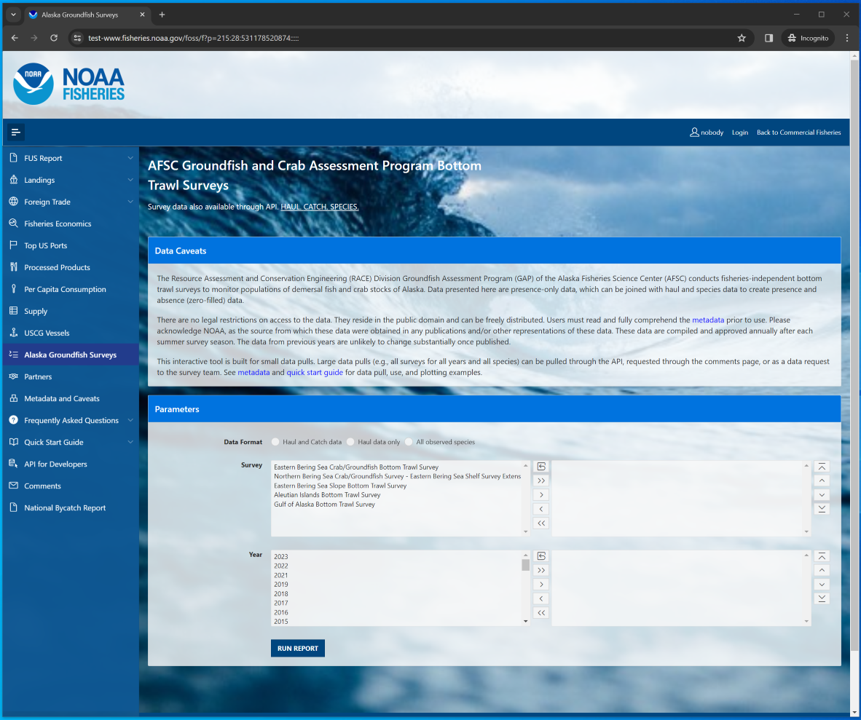
\includegraphics[width=6.24in,height=\textheight]{content/../img/foss_1_interface.png}

}

\caption{AFSC Groundfish and Crab Assessment Program Bottom Trawl Survey
data interface on the Fisheries One Stop Shop platform.}

\end{figure}

\hypertarget{select-and-filter}{%
\section{Select and filter}\label{select-and-filter}}

Select, filter, and package this and other NOAA Fisheries data from the
\href{https://www.fisheries.noaa.gov/foss}{Fisheries One Stop Shop
(FOSS)} platform. A user guide for the FOSS platform can be found
\href{https://www.fisheries.noaa.gov/foss/f?p=215:7:7542600605674:::::}{here}.
To begin a report, select options from the boxes what you need data for.

For a given box, select one or a few options from the ``options box''
(list on the left) to query by highlighting them. To select multiple
options, hold down the CTRL key while clicking on the options of
interest, or click and drag down the list. Once the options you wish to
be included in your query are highlighted, click the right-pointing
arrow (\texttt{\textgreater{}}) to move them into the ``selection box''
(list on the right). If you accidentally select an option that you do
not want to query, simply select the unwanted option from the selection
box and click the left-pointing arrow (\texttt{\textless{}}).

If you wish to select all options from the options box and send them to
the selection box, simply click the double right-pointing arrow
(\texttt{\textgreater{}\textgreater{}}). If you want to unselect all
options from the selection box, use the double left-pointing arrow
(\texttt{\textless{}\textless{}}) or the reset icon.

To find a specific species or group more quickly you can use the
\texttt{Search\ Species} option to quickly narrow the options. Search
for parts of species common names in the \texttt{Search\ Species} box by
entering a term and clicking the \texttt{search} button. The platform
will return a shorter list in the \texttt{Speices} options box of only
species that contain a match to that search term.

Use the \texttt{Reset\ All\ Parameters} button to reset all parameters
for entire form.

\begin{figure}

{\centering 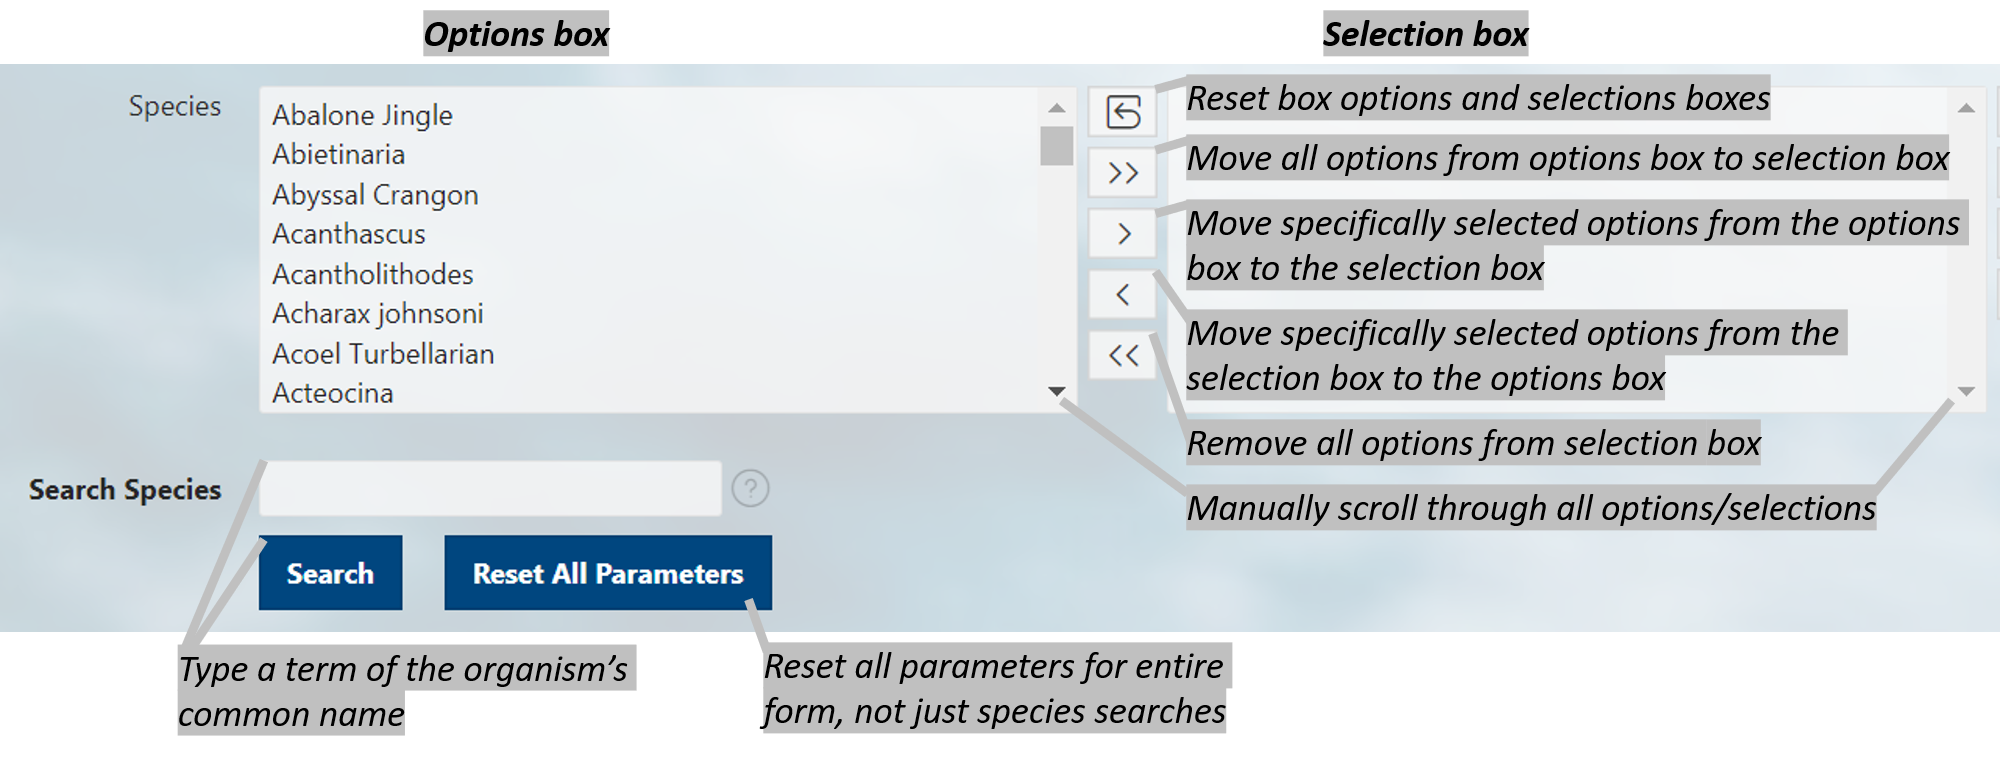
\includegraphics[width=6.67in,height=\textheight]{content/../img/foss_2_select.png}

}

\caption{Diagram of selection and search tools available on the FOSS
platofrom.}

\end{figure}

Filter options:

\begin{itemize}
\tightlist
\item
  \texttt{Survey}: Each survey has different in design, time series, and
  history. More information on each survey and their designs can be
  found in our
  \href{https://www.fisheries.noaa.gov/alaska/science-data/groundfish-assessment-program-bottom-trawl-surveys\#data-products}{annual
  data reports}.
\item
  \texttt{Year}: Surveys are not conducted in all years, so only data
  from the years for which the survey was conducted will be returned.
\item
  \texttt{Species}: Common name of all species ever encountered in the
  survey. Find more information about these species in our
  \href{https://www.fisheries.noaa.gov/resource/document/groundfish-survey-species-code-manual-and-data-codes-manual}{survey
  code books}.
\end{itemize}

\begin{quote}
In this example, we'll select for 2022 eastern Bering Sea Pacific cod
data. Here, we used the \texttt{Search\ Species} box to search for
species with the term ``cod'' in their common names and selected
``Pacific cod'' from that shortened list.
\end{quote}

\begin{figure}

{\centering 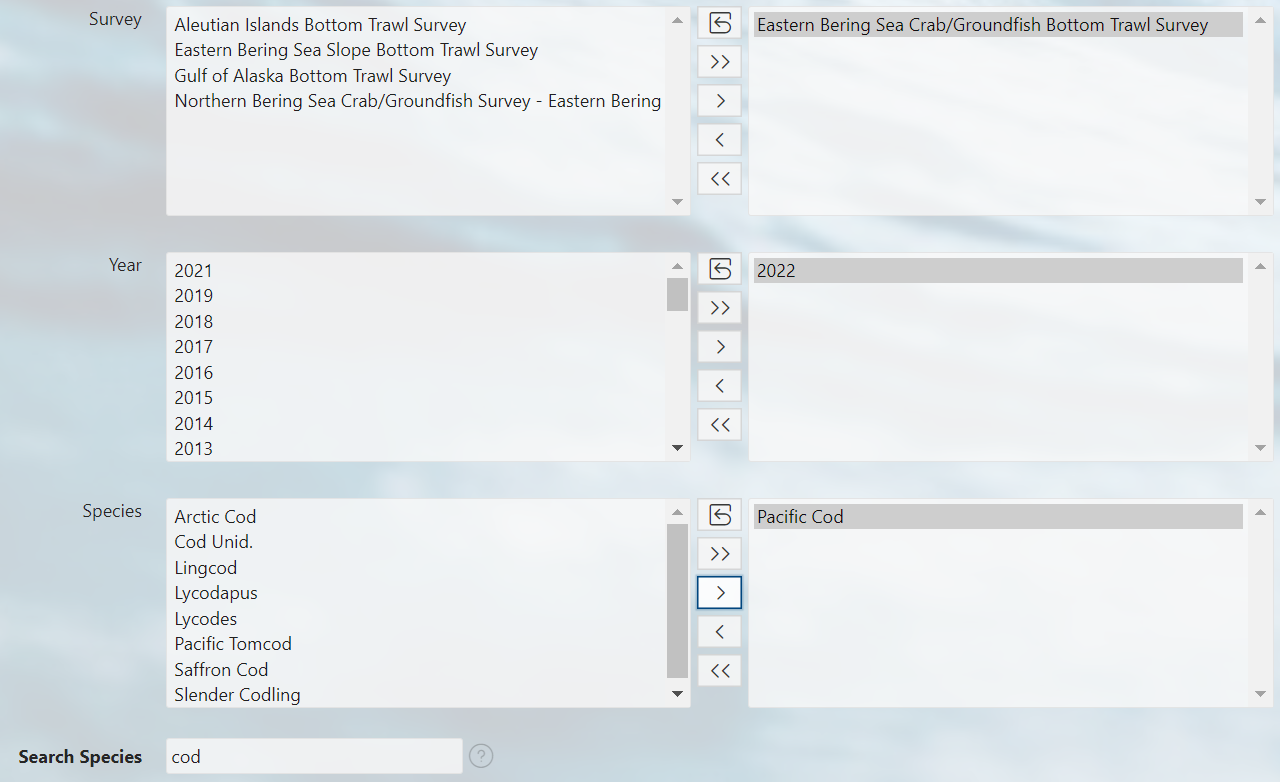
\includegraphics[width=4.27in,height=\textheight]{content/../img/foss_3_selected.png}

}

\caption{Diagram of selection and search tools available on the FOSS
platofrom.}

\end{figure}

\hypertarget{select-data-format}{%
\section{Select data format}\label{select-data-format}}

Select from the below radio list of pre-designed output tables. Once you
run the report, the user can further specify filter data and select
columns of interest. The tables below will only include data from the
selections made in the previous step.

\begin{itemize}
\tightlist
\item
  \texttt{All\ Data\ Fields:\ Presence\ and\ Absence\ (zero-filled)}:
  The most complete version of the data, including species, catch, haul,
  and environmental data. This data will include catch data for where
  species were caught and zeros for where the species were not caught.
  This is important for calculating catch-per-unit-effort data,
  preparing distribution plots (e.g.,
  \href{https://github.com/afsc-gap-products/akgfmaps}{using the
  akgfmaps R package}), and many statistical analyses.
\item
  \texttt{All\ Data\ Fields:\ Presence-only\ (non-zero)}: The second
  most complete version of the data, including species, catch, haul, and
  environmental data. However, this data only includes catch data for
  where species were caught and does not include zeros for where the
  species were not caught. This will return smaller, more focused data
  and can be useful for quickly assessing how many species were caught
  or how many stations species were caught at.
\item
  \texttt{Catch\ data:\ Presence\ and\ Absence\ (zero-filled)}: This
  data set is similar to
  \texttt{All\ Data\ Fields:\ Presence\ and\ Absence\ (zero-filled)},
  but only includes catch and species data columns.
\item
  \texttt{Catch\ data:\ Presence-only\ (non-zero)}: This data set is
  similar to \texttt{All\ Data\ Fields:\ Presence-only\ (non-zero)}, but
  only includes catch and species data columns.
\item
  \texttt{Haul\ Data}: This data set only includes haul and
  environmental data collected from the survey. This data will only
  include one observation per haul event/station.
\end{itemize}

\begin{quote}
In this example, we'll select
\texttt{All\ Data\ Fields:\ Presence\ and\ Absence\ (zero-filled).}
\end{quote}

\begin{figure}

{\centering 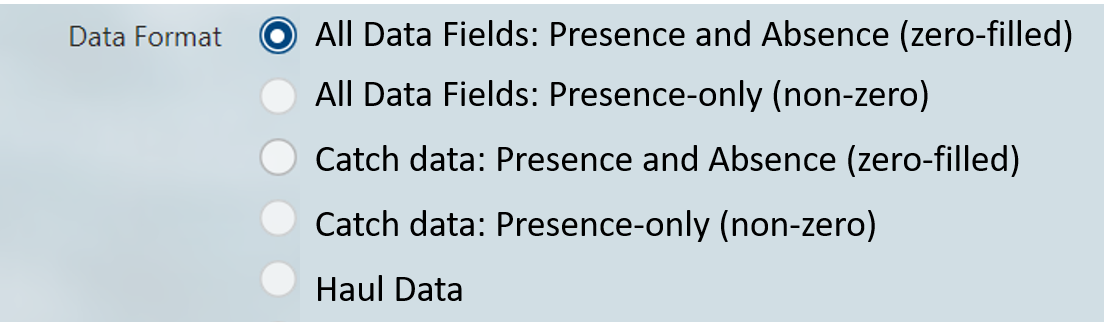
\includegraphics[width=3.68in,height=\textheight]{content/../img/foss_4_data_format.png}

}

\caption{Diagram of the pre-set data format options.}

\end{figure}

\hypertarget{run-report}{%
\section{Run report}\label{run-report}}

Click the \texttt{RUN\ REPORT} button. Below the select and filter area,
the results of your query will appear below the page in the format you
selected. To change the format, make a different selection and run the
report again. Further modifications to your results can be made by
clicking on the \texttt{Actions} button above your data. Here you can
\texttt{download} your data, \texttt{select\ columns} included in your
results, and apply a variety of \texttt{filters} and mathematical tools.

\begin{figure}

{\centering 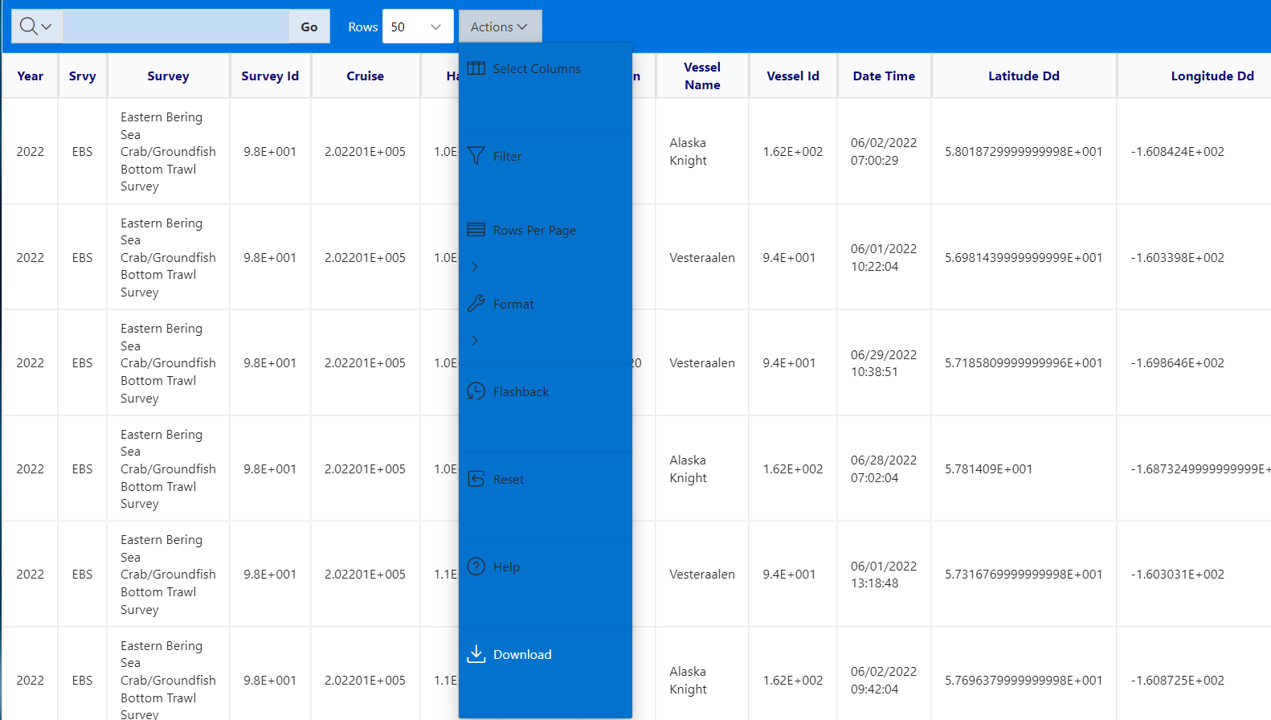
\includegraphics[width=4.24in,height=\textheight]{content/../img/foss_5_run_report.png}

}

\caption{Example data returned from running the report.}

\end{figure}

\hypertarget{access-api-data-using-r}{%
\chapter{Access API data using R}\label{access-api-data-using-r}}

An application programming interface (API) is a way for two or more
computer programs to communicate with each other.

More information about how to amend API links can be found
\href{https://docs.oracle.com/en/database/oracle/oracle-rest-data-services/22.3/books.html\#AELIG90103/}{here}.
Useful introductions to using APIs in \texttt{R} can be found
\href{https://www.dataquest.io/blog/r-api-tutorial/}{here}.

\hypertarget{ex.-1-load-the-first-25-rows-default-of-data}{%
\section{Ex. 1: Load the first 25 rows (default) of
data}\label{ex.-1-load-the-first-25-rows-default-of-data}}

\begin{Shaded}
\begin{Highlighting}[]
 \CommentTok{\# install.packages(c("httr", "jsonlite"))}
\FunctionTok{library}\NormalTok{(httr)}
\FunctionTok{library}\NormalTok{(jsonlite)}
\FunctionTok{library}\NormalTok{(dplyr)}
 \CommentTok{\# link to the API}
\NormalTok{api\_link }\OtherTok{\textless{}{-}} \StringTok{"https://apps{-}st.fisheries.noaa.gov/ods/foss/afsc\_groundfish\_survey/"}

\NormalTok{res }\OtherTok{\textless{}{-}}\NormalTok{ httr}\SpecialCharTok{::}\FunctionTok{GET}\NormalTok{(}\AttributeTok{url =}\NormalTok{ api\_link)}
 \CommentTok{\# res \# Test connection}
\NormalTok{data }\OtherTok{\textless{}{-}}\NormalTok{ jsonlite}\SpecialCharTok{::}\FunctionTok{fromJSON}\NormalTok{(base}\SpecialCharTok{::}\FunctionTok{rawToChar}\NormalTok{(res}\SpecialCharTok{$}\NormalTok{content))}
 \CommentTok{\# names(data)}
\NormalTok{flextable}\SpecialCharTok{::}\FunctionTok{flextable}\NormalTok{(}\FunctionTok{head}\NormalTok{(data}\SpecialCharTok{$}\NormalTok{items, }\DecValTok{3}\NormalTok{)) }
\end{Highlighting}
\end{Shaded}

\global\setlength{\Oldarrayrulewidth}{\arrayrulewidth}

\global\setlength{\Oldtabcolsep}{\tabcolsep}

\setlength{\tabcolsep}{0pt}

\renewcommand*{\arraystretch}{1.5}



\providecommand{\ascline}[3]{\noalign{\global\arrayrulewidth #1}\arrayrulecolor[HTML]{#2}\cline{#3}}

\begin{longtable}[c]{|p{0.75in}|p{0.75in}|p{0.75in}|p{0.75in}|p{0.75in}|p{0.75in}|p{0.75in}|p{0.75in}|p{0.75in}|p{0.75in}|p{0.75in}|p{0.75in}|p{0.75in}|p{0.75in}|p{0.75in}|p{0.75in}|p{0.75in}|p{0.75in}|p{0.75in}|p{0.75in}|p{0.75in}|p{0.75in}|p{0.75in}|p{0.75in}|p{0.75in}|p{0.75in}|p{0.75in}|p{0.75in}|p{0.75in}|p{0.75in}|p{0.75in}|p{0.75in}|p{0.75in}|p{0.75in}|p{0.75in}|p{0.75in}}

\caption{Ex. 1: Load the first 25 rows (default) of data.} \\ 


\ascline{1.5pt}{666666}{1-36}

\multicolumn{1}{>{\raggedleft}m{\dimexpr 0.75in+0\tabcolsep}}{\textcolor[HTML]{000000}{\fontsize{11}{11}\selectfont{year}}} & \multicolumn{1}{>{\raggedright}m{\dimexpr 0.75in+0\tabcolsep}}{\textcolor[HTML]{000000}{\fontsize{11}{11}\selectfont{srvy}}} & \multicolumn{1}{>{\raggedright}m{\dimexpr 0.75in+0\tabcolsep}}{\textcolor[HTML]{000000}{\fontsize{11}{11}\selectfont{survey}}} & \multicolumn{1}{>{\raggedright}m{\dimexpr 0.75in+0\tabcolsep}}{\textcolor[HTML]{000000}{\fontsize{11}{11}\selectfont{survey\_id}}} & \multicolumn{1}{>{\raggedright}m{\dimexpr 0.75in+0\tabcolsep}}{\textcolor[HTML]{000000}{\fontsize{11}{11}\selectfont{cruise}}} & \multicolumn{1}{>{\raggedright}m{\dimexpr 0.75in+0\tabcolsep}}{\textcolor[HTML]{000000}{\fontsize{11}{11}\selectfont{haul}}} & \multicolumn{1}{>{\raggedright}m{\dimexpr 0.75in+0\tabcolsep}}{\textcolor[HTML]{000000}{\fontsize{11}{11}\selectfont{stratum}}} & \multicolumn{1}{>{\raggedright}m{\dimexpr 0.75in+0\tabcolsep}}{\textcolor[HTML]{000000}{\fontsize{11}{11}\selectfont{station}}} & \multicolumn{1}{>{\raggedright}m{\dimexpr 0.75in+0\tabcolsep}}{\textcolor[HTML]{000000}{\fontsize{11}{11}\selectfont{vessel\_name}}} & \multicolumn{1}{>{\raggedright}m{\dimexpr 0.75in+0\tabcolsep}}{\textcolor[HTML]{000000}{\fontsize{11}{11}\selectfont{vessel\_id}}} & \multicolumn{1}{>{\raggedright}m{\dimexpr 0.75in+0\tabcolsep}}{\textcolor[HTML]{000000}{\fontsize{11}{11}\selectfont{date\_time}}} & \multicolumn{1}{>{\raggedright}m{\dimexpr 0.75in+0\tabcolsep}}{\textcolor[HTML]{000000}{\fontsize{11}{11}\selectfont{latitude\_dd}}} & \multicolumn{1}{>{\raggedright}m{\dimexpr 0.75in+0\tabcolsep}}{\textcolor[HTML]{000000}{\fontsize{11}{11}\selectfont{longitude\_dd}}} & \multicolumn{1}{>{\raggedright}m{\dimexpr 0.75in+0\tabcolsep}}{\textcolor[HTML]{000000}{\fontsize{11}{11}\selectfont{species\_code}}} & \multicolumn{1}{>{\raggedright}m{\dimexpr 0.75in+0\tabcolsep}}{\textcolor[HTML]{000000}{\fontsize{11}{11}\selectfont{common\_name}}} & \multicolumn{1}{>{\raggedright}m{\dimexpr 0.75in+0\tabcolsep}}{\textcolor[HTML]{000000}{\fontsize{11}{11}\selectfont{scientific\_name}}} & \multicolumn{1}{>{\raggedright}m{\dimexpr 0.75in+0\tabcolsep}}{\textcolor[HTML]{000000}{\fontsize{11}{11}\selectfont{taxon\_confidence}}} & \multicolumn{1}{>{\raggedright}m{\dimexpr 0.75in+0\tabcolsep}}{\textcolor[HTML]{000000}{\fontsize{11}{11}\selectfont{cpue\_kgha}}} & \multicolumn{1}{>{\raggedright}m{\dimexpr 0.75in+0\tabcolsep}}{\textcolor[HTML]{000000}{\fontsize{11}{11}\selectfont{cpue\_kgkm2}}} & \multicolumn{1}{>{\raggedright}m{\dimexpr 0.75in+0\tabcolsep}}{\textcolor[HTML]{000000}{\fontsize{11}{11}\selectfont{cpue\_kg1000km2}}} & \multicolumn{1}{>{\raggedright}m{\dimexpr 0.75in+0\tabcolsep}}{\textcolor[HTML]{000000}{\fontsize{11}{11}\selectfont{cpue\_noha}}} & \multicolumn{1}{>{\raggedright}m{\dimexpr 0.75in+0\tabcolsep}}{\textcolor[HTML]{000000}{\fontsize{11}{11}\selectfont{cpue\_nokm2}}} & \multicolumn{1}{>{\raggedright}m{\dimexpr 0.75in+0\tabcolsep}}{\textcolor[HTML]{000000}{\fontsize{11}{11}\selectfont{cpue\_no1000km2}}} & \multicolumn{1}{>{\raggedright}m{\dimexpr 0.75in+0\tabcolsep}}{\textcolor[HTML]{000000}{\fontsize{11}{11}\selectfont{weight\_kg}}} & \multicolumn{1}{>{\raggedright}m{\dimexpr 0.75in+0\tabcolsep}}{\textcolor[HTML]{000000}{\fontsize{11}{11}\selectfont{count}}} & \multicolumn{1}{>{\raggedright}m{\dimexpr 0.75in+0\tabcolsep}}{\textcolor[HTML]{000000}{\fontsize{11}{11}\selectfont{bottom\_temperature\_c}}} & \multicolumn{1}{>{\raggedright}m{\dimexpr 0.75in+0\tabcolsep}}{\textcolor[HTML]{000000}{\fontsize{11}{11}\selectfont{surface\_temperature\_c}}} & \multicolumn{1}{>{\raggedright}m{\dimexpr 0.75in+0\tabcolsep}}{\textcolor[HTML]{000000}{\fontsize{11}{11}\selectfont{depth\_m}}} & \multicolumn{1}{>{\raggedright}m{\dimexpr 0.75in+0\tabcolsep}}{\textcolor[HTML]{000000}{\fontsize{11}{11}\selectfont{distance\_fished\_km}}} & \multicolumn{1}{>{\raggedright}m{\dimexpr 0.75in+0\tabcolsep}}{\textcolor[HTML]{000000}{\fontsize{11}{11}\selectfont{net\_width\_m}}} & \multicolumn{1}{>{\raggedright}m{\dimexpr 0.75in+0\tabcolsep}}{\textcolor[HTML]{000000}{\fontsize{11}{11}\selectfont{net\_height\_m}}} & \multicolumn{1}{>{\raggedright}m{\dimexpr 0.75in+0\tabcolsep}}{\textcolor[HTML]{000000}{\fontsize{11}{11}\selectfont{area\_swept\_ha}}} & \multicolumn{1}{>{\raggedright}m{\dimexpr 0.75in+0\tabcolsep}}{\textcolor[HTML]{000000}{\fontsize{11}{11}\selectfont{duration\_hr}}} & \multicolumn{1}{>{\raggedleft}m{\dimexpr 0.75in+0\tabcolsep}}{\textcolor[HTML]{000000}{\fontsize{11}{11}\selectfont{tsn}}} & \multicolumn{1}{>{\raggedleft}m{\dimexpr 0.75in+0\tabcolsep}}{\textcolor[HTML]{000000}{\fontsize{11}{11}\selectfont{ak\_survey\_id}}} & \multicolumn{1}{>{\raggedleft}m{\dimexpr 0.75in+0\tabcolsep}}{\textcolor[HTML]{000000}{\fontsize{11}{11}\selectfont{links}}} \\

\ascline{1.5pt}{666666}{1-36}\endhead



\multicolumn{1}{>{\raggedleft}m{\dimexpr 0.75in+0\tabcolsep}}{\textcolor[HTML]{000000}{\fontsize{11}{11}\selectfont{2,002}}} & \multicolumn{1}{>{\raggedright}m{\dimexpr 0.75in+0\tabcolsep}}{\textcolor[HTML]{000000}{\fontsize{11}{11}\selectfont{AI}}} & \multicolumn{1}{>{\raggedright}m{\dimexpr 0.75in+0\tabcolsep}}{\textcolor[HTML]{000000}{\fontsize{11}{11}\selectfont{Aleutian\ Islands\ Bottom\ Trawl\ Survey}}} & \multicolumn{1}{>{\raggedright}m{\dimexpr 0.75in+0\tabcolsep}}{\textcolor[HTML]{000000}{\fontsize{11}{11}\selectfont{5.2E+001}}} & \multicolumn{1}{>{\raggedright}m{\dimexpr 0.75in+0\tabcolsep}}{\textcolor[HTML]{000000}{\fontsize{11}{11}\selectfont{2.00201E+005}}} & \multicolumn{1}{>{\raggedright}m{\dimexpr 0.75in+0\tabcolsep}}{\textcolor[HTML]{000000}{\fontsize{11}{11}\selectfont{6.0E+000}}} & \multicolumn{1}{>{\raggedright}m{\dimexpr 0.75in+0\tabcolsep}}{\textcolor[HTML]{000000}{\fontsize{11}{11}\selectfont{7.22E+002}}} & \multicolumn{1}{>{\raggedright}m{\dimexpr 0.75in+0\tabcolsep}}{\textcolor[HTML]{000000}{\fontsize{11}{11}\selectfont{307-63}}} & \multicolumn{1}{>{\raggedright}m{\dimexpr 0.75in+0\tabcolsep}}{\textcolor[HTML]{000000}{\fontsize{11}{11}\selectfont{Vesteraalen}}} & \multicolumn{1}{>{\raggedright}m{\dimexpr 0.75in+0\tabcolsep}}{\textcolor[HTML]{000000}{\fontsize{11}{11}\selectfont{9.4E+001}}} & \multicolumn{1}{>{\raggedright}m{\dimexpr 0.75in+0\tabcolsep}}{\textcolor[HTML]{000000}{\fontsize{11}{11}\selectfont{05/17/2002\ 18:56:58}}} & \multicolumn{1}{>{\raggedright}m{\dimexpr 0.75in+0\tabcolsep}}{\textcolor[HTML]{000000}{\fontsize{11}{11}\selectfont{5.3737209999999997E+001}}} & \multicolumn{1}{>{\raggedright}m{\dimexpr 0.75in+0\tabcolsep}}{\textcolor[HTML]{000000}{\fontsize{11}{11}\selectfont{-1.6701570000000001E+002}}} & \multicolumn{1}{>{\raggedright}m{\dimexpr 0.75in+0\tabcolsep}}{\textcolor[HTML]{000000}{\fontsize{11}{11}\selectfont{9.502E+004}}} & \multicolumn{1}{>{\raggedright}m{\dimexpr 0.75in+0\tabcolsep}}{\textcolor[HTML]{000000}{\fontsize{11}{11}\selectfont{feathery\ bryozoan}}} & \multicolumn{1}{>{\raggedright}m{\dimexpr 0.75in+0\tabcolsep}}{\textcolor[HTML]{000000}{\fontsize{11}{11}\selectfont{Eucratea\ loricata}}} & \multicolumn{1}{>{\raggedright}m{\dimexpr 0.75in+0\tabcolsep}}{\textcolor[HTML]{000000}{\fontsize{11}{11}\selectfont{Low}}} & \multicolumn{1}{>{\raggedright}m{\dimexpr 0.75in+0\tabcolsep}}{\textcolor[HTML]{000000}{\fontsize{11}{11}\selectfont{1.7493999999999999E-002}}} & \multicolumn{1}{>{\raggedright}m{\dimexpr 0.75in+0\tabcolsep}}{\textcolor[HTML]{000000}{\fontsize{11}{11}\selectfont{1.7494449999999999E+000}}} & \multicolumn{1}{>{\raggedright}m{\dimexpr 0.75in+0\tabcolsep}}{\textcolor[HTML]{000000}{\fontsize{11}{11}\selectfont{1.7494451079999999E+003}}} & \multicolumn{1}{>{\raggedright}m{\dimexpr 0.75in+0\tabcolsep}}{\textcolor[HTML]{000000}{\fontsize{11}{11}\selectfont{}}} & \multicolumn{1}{>{\raggedright}m{\dimexpr 0.75in+0\tabcolsep}}{\textcolor[HTML]{000000}{\fontsize{11}{11}\selectfont{}}} & \multicolumn{1}{>{\raggedright}m{\dimexpr 0.75in+0\tabcolsep}}{\textcolor[HTML]{000000}{\fontsize{11}{11}\selectfont{}}} & \multicolumn{1}{>{\raggedright}m{\dimexpr 0.75in+0\tabcolsep}}{\textcolor[HTML]{000000}{\fontsize{11}{11}\selectfont{4.3999999999999997E-002}}} & \multicolumn{1}{>{\raggedright}m{\dimexpr 0.75in+0\tabcolsep}}{\textcolor[HTML]{000000}{\fontsize{11}{11}\selectfont{0}}} & \multicolumn{1}{>{\raggedright}m{\dimexpr 0.75in+0\tabcolsep}}{\textcolor[HTML]{000000}{\fontsize{11}{11}\selectfont{4.0999999999999996E+000}}} & \multicolumn{1}{>{\raggedright}m{\dimexpr 0.75in+0\tabcolsep}}{\textcolor[HTML]{000000}{\fontsize{11}{11}\selectfont{5.2999999999999998E+000}}} & \multicolumn{1}{>{\raggedright}m{\dimexpr 0.75in+0\tabcolsep}}{\textcolor[HTML]{000000}{\fontsize{11}{11}\selectfont{1.87E+002}}} & \multicolumn{1}{>{\raggedright}m{\dimexpr 0.75in+0\tabcolsep}}{\textcolor[HTML]{000000}{\fontsize{11}{11}\selectfont{1.5609999999999999E+000}}} & \multicolumn{1}{>{\raggedright}m{\dimexpr 0.75in+0\tabcolsep}}{\textcolor[HTML]{000000}{\fontsize{11}{11}\selectfont{1.6111999999999998E+001}}} & \multicolumn{1}{>{\raggedright}m{\dimexpr 0.75in+0\tabcolsep}}{\textcolor[HTML]{000000}{\fontsize{11}{11}\selectfont{7.25E+000}}} & \multicolumn{1}{>{\raggedright}m{\dimexpr 0.75in+0\tabcolsep}}{\textcolor[HTML]{000000}{\fontsize{11}{11}\selectfont{2.5150831999999994E+000}}} & \multicolumn{1}{>{\raggedright}m{\dimexpr 0.75in+0\tabcolsep}}{\textcolor[HTML]{000000}{\fontsize{11}{11}\selectfont{2.8000000000000003E-001}}} & \multicolumn{1}{>{\raggedleft}m{\dimexpr 0.75in+0\tabcolsep}}{\textcolor[HTML]{000000}{\fontsize{11}{11}\selectfont{155,809}}} & \multicolumn{1}{>{\raggedleft}m{\dimexpr 0.75in+0\tabcolsep}}{\textcolor[HTML]{000000}{\fontsize{11}{11}\selectfont{878,821}}} & \multicolumn{1}{>{\raggedleft}m{\dimexpr 0.75in+0\tabcolsep}}{\textcolor[HTML]{000000}{\fontsize{11}{11}\selectfont{[[data.frame]]}}} \\





\multicolumn{1}{>{\raggedleft}m{\dimexpr 0.75in+0\tabcolsep}}{\textcolor[HTML]{000000}{\fontsize{11}{11}\selectfont{2,002}}} & \multicolumn{1}{>{\raggedright}m{\dimexpr 0.75in+0\tabcolsep}}{\textcolor[HTML]{000000}{\fontsize{11}{11}\selectfont{AI}}} & \multicolumn{1}{>{\raggedright}m{\dimexpr 0.75in+0\tabcolsep}}{\textcolor[HTML]{000000}{\fontsize{11}{11}\selectfont{Aleutian\ Islands\ Bottom\ Trawl\ Survey}}} & \multicolumn{1}{>{\raggedright}m{\dimexpr 0.75in+0\tabcolsep}}{\textcolor[HTML]{000000}{\fontsize{11}{11}\selectfont{5.2E+001}}} & \multicolumn{1}{>{\raggedright}m{\dimexpr 0.75in+0\tabcolsep}}{\textcolor[HTML]{000000}{\fontsize{11}{11}\selectfont{2.00201E+005}}} & \multicolumn{1}{>{\raggedright}m{\dimexpr 0.75in+0\tabcolsep}}{\textcolor[HTML]{000000}{\fontsize{11}{11}\selectfont{6.0E+000}}} & \multicolumn{1}{>{\raggedright}m{\dimexpr 0.75in+0\tabcolsep}}{\textcolor[HTML]{000000}{\fontsize{11}{11}\selectfont{7.22E+002}}} & \multicolumn{1}{>{\raggedright}m{\dimexpr 0.75in+0\tabcolsep}}{\textcolor[HTML]{000000}{\fontsize{11}{11}\selectfont{307-63}}} & \multicolumn{1}{>{\raggedright}m{\dimexpr 0.75in+0\tabcolsep}}{\textcolor[HTML]{000000}{\fontsize{11}{11}\selectfont{Vesteraalen}}} & \multicolumn{1}{>{\raggedright}m{\dimexpr 0.75in+0\tabcolsep}}{\textcolor[HTML]{000000}{\fontsize{11}{11}\selectfont{9.4E+001}}} & \multicolumn{1}{>{\raggedright}m{\dimexpr 0.75in+0\tabcolsep}}{\textcolor[HTML]{000000}{\fontsize{11}{11}\selectfont{05/17/2002\ 18:56:58}}} & \multicolumn{1}{>{\raggedright}m{\dimexpr 0.75in+0\tabcolsep}}{\textcolor[HTML]{000000}{\fontsize{11}{11}\selectfont{5.3737209999999997E+001}}} & \multicolumn{1}{>{\raggedright}m{\dimexpr 0.75in+0\tabcolsep}}{\textcolor[HTML]{000000}{\fontsize{11}{11}\selectfont{-1.6701570000000001E+002}}} & \multicolumn{1}{>{\raggedright}m{\dimexpr 0.75in+0\tabcolsep}}{\textcolor[HTML]{000000}{\fontsize{11}{11}\selectfont{7.9E+004}}} & \multicolumn{1}{>{\raggedright}m{\dimexpr 0.75in+0\tabcolsep}}{\textcolor[HTML]{000000}{\fontsize{11}{11}\selectfont{squid\ unid.}}} & \multicolumn{1}{>{\raggedright}m{\dimexpr 0.75in+0\tabcolsep}}{\textcolor[HTML]{000000}{\fontsize{11}{11}\selectfont{Decapodiformes}}} & \multicolumn{1}{>{\raggedright}m{\dimexpr 0.75in+0\tabcolsep}}{\textcolor[HTML]{000000}{\fontsize{11}{11}\selectfont{High}}} & \multicolumn{1}{>{\raggedright}m{\dimexpr 0.75in+0\tabcolsep}}{\textcolor[HTML]{000000}{\fontsize{11}{11}\selectfont{2.2266000000000001E-002}}} & \multicolumn{1}{>{\raggedright}m{\dimexpr 0.75in+0\tabcolsep}}{\textcolor[HTML]{000000}{\fontsize{11}{11}\selectfont{2.2265670000000002E+000}}} & \multicolumn{1}{>{\raggedright}m{\dimexpr 0.75in+0\tabcolsep}}{\textcolor[HTML]{000000}{\fontsize{11}{11}\selectfont{2.2265665009999998E+003}}} & \multicolumn{1}{>{\raggedright}m{\dimexpr 0.75in+0\tabcolsep}}{\textcolor[HTML]{000000}{\fontsize{11}{11}\selectfont{3.180809E+000}}} & \multicolumn{1}{>{\raggedright}m{\dimexpr 0.75in+0\tabcolsep}}{\textcolor[HTML]{000000}{\fontsize{11}{11}\selectfont{3.1808092900000003E+002}}} & \multicolumn{1}{>{\raggedright}m{\dimexpr 0.75in+0\tabcolsep}}{\textcolor[HTML]{000000}{\fontsize{11}{11}\selectfont{3.1808092869500001E+005}}} & \multicolumn{1}{>{\raggedright}m{\dimexpr 0.75in+0\tabcolsep}}{\textcolor[HTML]{000000}{\fontsize{11}{11}\selectfont{5.6000000000000001E-002}}} & \multicolumn{1}{>{\raggedright}m{\dimexpr 0.75in+0\tabcolsep}}{\textcolor[HTML]{000000}{\fontsize{11}{11}\selectfont{8.0E+000}}} & \multicolumn{1}{>{\raggedright}m{\dimexpr 0.75in+0\tabcolsep}}{\textcolor[HTML]{000000}{\fontsize{11}{11}\selectfont{4.0999999999999996E+000}}} & \multicolumn{1}{>{\raggedright}m{\dimexpr 0.75in+0\tabcolsep}}{\textcolor[HTML]{000000}{\fontsize{11}{11}\selectfont{5.2999999999999998E+000}}} & \multicolumn{1}{>{\raggedright}m{\dimexpr 0.75in+0\tabcolsep}}{\textcolor[HTML]{000000}{\fontsize{11}{11}\selectfont{1.87E+002}}} & \multicolumn{1}{>{\raggedright}m{\dimexpr 0.75in+0\tabcolsep}}{\textcolor[HTML]{000000}{\fontsize{11}{11}\selectfont{1.5609999999999999E+000}}} & \multicolumn{1}{>{\raggedright}m{\dimexpr 0.75in+0\tabcolsep}}{\textcolor[HTML]{000000}{\fontsize{11}{11}\selectfont{1.6111999999999998E+001}}} & \multicolumn{1}{>{\raggedright}m{\dimexpr 0.75in+0\tabcolsep}}{\textcolor[HTML]{000000}{\fontsize{11}{11}\selectfont{7.25E+000}}} & \multicolumn{1}{>{\raggedright}m{\dimexpr 0.75in+0\tabcolsep}}{\textcolor[HTML]{000000}{\fontsize{11}{11}\selectfont{2.5150831999999994E+000}}} & \multicolumn{1}{>{\raggedright}m{\dimexpr 0.75in+0\tabcolsep}}{\textcolor[HTML]{000000}{\fontsize{11}{11}\selectfont{2.8000000000000003E-001}}} & \multicolumn{1}{>{\raggedleft}m{\dimexpr 0.75in+0\tabcolsep}}{\textcolor[HTML]{000000}{\fontsize{11}{11}\selectfont{}}} & \multicolumn{1}{>{\raggedleft}m{\dimexpr 0.75in+0\tabcolsep}}{\textcolor[HTML]{000000}{\fontsize{11}{11}\selectfont{878,822}}} & \multicolumn{1}{>{\raggedleft}m{\dimexpr 0.75in+0\tabcolsep}}{\textcolor[HTML]{000000}{\fontsize{11}{11}\selectfont{[[data.frame]]}}} \\





\multicolumn{1}{>{\raggedleft}m{\dimexpr 0.75in+0\tabcolsep}}{\textcolor[HTML]{000000}{\fontsize{11}{11}\selectfont{2,002}}} & \multicolumn{1}{>{\raggedright}m{\dimexpr 0.75in+0\tabcolsep}}{\textcolor[HTML]{000000}{\fontsize{11}{11}\selectfont{AI}}} & \multicolumn{1}{>{\raggedright}m{\dimexpr 0.75in+0\tabcolsep}}{\textcolor[HTML]{000000}{\fontsize{11}{11}\selectfont{Aleutian\ Islands\ Bottom\ Trawl\ Survey}}} & \multicolumn{1}{>{\raggedright}m{\dimexpr 0.75in+0\tabcolsep}}{\textcolor[HTML]{000000}{\fontsize{11}{11}\selectfont{5.2E+001}}} & \multicolumn{1}{>{\raggedright}m{\dimexpr 0.75in+0\tabcolsep}}{\textcolor[HTML]{000000}{\fontsize{11}{11}\selectfont{2.00201E+005}}} & \multicolumn{1}{>{\raggedright}m{\dimexpr 0.75in+0\tabcolsep}}{\textcolor[HTML]{000000}{\fontsize{11}{11}\selectfont{6.0E+000}}} & \multicolumn{1}{>{\raggedright}m{\dimexpr 0.75in+0\tabcolsep}}{\textcolor[HTML]{000000}{\fontsize{11}{11}\selectfont{7.22E+002}}} & \multicolumn{1}{>{\raggedright}m{\dimexpr 0.75in+0\tabcolsep}}{\textcolor[HTML]{000000}{\fontsize{11}{11}\selectfont{307-63}}} & \multicolumn{1}{>{\raggedright}m{\dimexpr 0.75in+0\tabcolsep}}{\textcolor[HTML]{000000}{\fontsize{11}{11}\selectfont{Vesteraalen}}} & \multicolumn{1}{>{\raggedright}m{\dimexpr 0.75in+0\tabcolsep}}{\textcolor[HTML]{000000}{\fontsize{11}{11}\selectfont{9.4E+001}}} & \multicolumn{1}{>{\raggedright}m{\dimexpr 0.75in+0\tabcolsep}}{\textcolor[HTML]{000000}{\fontsize{11}{11}\selectfont{05/17/2002\ 18:56:58}}} & \multicolumn{1}{>{\raggedright}m{\dimexpr 0.75in+0\tabcolsep}}{\textcolor[HTML]{000000}{\fontsize{11}{11}\selectfont{5.3737209999999997E+001}}} & \multicolumn{1}{>{\raggedright}m{\dimexpr 0.75in+0\tabcolsep}}{\textcolor[HTML]{000000}{\fontsize{11}{11}\selectfont{-1.6701570000000001E+002}}} & \multicolumn{1}{>{\raggedright}m{\dimexpr 0.75in+0\tabcolsep}}{\textcolor[HTML]{000000}{\fontsize{11}{11}\selectfont{2.4191E+004}}} & \multicolumn{1}{>{\raggedright}m{\dimexpr 0.75in+0\tabcolsep}}{\textcolor[HTML]{000000}{\fontsize{11}{11}\selectfont{shortfin\ eelpout}}} & \multicolumn{1}{>{\raggedright}m{\dimexpr 0.75in+0\tabcolsep}}{\textcolor[HTML]{000000}{\fontsize{11}{11}\selectfont{Lycodes\ brevipes}}} & \multicolumn{1}{>{\raggedright}m{\dimexpr 0.75in+0\tabcolsep}}{\textcolor[HTML]{000000}{\fontsize{11}{11}\selectfont{High}}} & \multicolumn{1}{>{\raggedright}m{\dimexpr 0.75in+0\tabcolsep}}{\textcolor[HTML]{000000}{\fontsize{11}{11}\selectfont{3.5784000000000003E-002}}} & \multicolumn{1}{>{\raggedright}m{\dimexpr 0.75in+0\tabcolsep}}{\textcolor[HTML]{000000}{\fontsize{11}{11}\selectfont{3.5784099999999999E+000}}} & \multicolumn{1}{>{\raggedright}m{\dimexpr 0.75in+0\tabcolsep}}{\textcolor[HTML]{000000}{\fontsize{11}{11}\selectfont{3.5784104480000001E+003}}} & \multicolumn{1}{>{\raggedright}m{\dimexpr 0.75in+0\tabcolsep}}{\textcolor[HTML]{000000}{\fontsize{11}{11}\selectfont{7.9520199999999996E-001}}} & \multicolumn{1}{>{\raggedright}m{\dimexpr 0.75in+0\tabcolsep}}{\textcolor[HTML]{000000}{\fontsize{11}{11}\selectfont{7.9520231999999993E+001}}} & \multicolumn{1}{>{\raggedright}m{\dimexpr 0.75in+0\tabcolsep}}{\textcolor[HTML]{000000}{\fontsize{11}{11}\selectfont{7.9520232174000004E+004}}} & \multicolumn{1}{>{\raggedright}m{\dimexpr 0.75in+0\tabcolsep}}{\textcolor[HTML]{000000}{\fontsize{11}{11}\selectfont{8.9999999999999997E-002}}} & \multicolumn{1}{>{\raggedright}m{\dimexpr 0.75in+0\tabcolsep}}{\textcolor[HTML]{000000}{\fontsize{11}{11}\selectfont{2.0E+000}}} & \multicolumn{1}{>{\raggedright}m{\dimexpr 0.75in+0\tabcolsep}}{\textcolor[HTML]{000000}{\fontsize{11}{11}\selectfont{4.0999999999999996E+000}}} & \multicolumn{1}{>{\raggedright}m{\dimexpr 0.75in+0\tabcolsep}}{\textcolor[HTML]{000000}{\fontsize{11}{11}\selectfont{5.2999999999999998E+000}}} & \multicolumn{1}{>{\raggedright}m{\dimexpr 0.75in+0\tabcolsep}}{\textcolor[HTML]{000000}{\fontsize{11}{11}\selectfont{1.87E+002}}} & \multicolumn{1}{>{\raggedright}m{\dimexpr 0.75in+0\tabcolsep}}{\textcolor[HTML]{000000}{\fontsize{11}{11}\selectfont{1.5609999999999999E+000}}} & \multicolumn{1}{>{\raggedright}m{\dimexpr 0.75in+0\tabcolsep}}{\textcolor[HTML]{000000}{\fontsize{11}{11}\selectfont{1.6111999999999998E+001}}} & \multicolumn{1}{>{\raggedright}m{\dimexpr 0.75in+0\tabcolsep}}{\textcolor[HTML]{000000}{\fontsize{11}{11}\selectfont{7.25E+000}}} & \multicolumn{1}{>{\raggedright}m{\dimexpr 0.75in+0\tabcolsep}}{\textcolor[HTML]{000000}{\fontsize{11}{11}\selectfont{2.5150831999999994E+000}}} & \multicolumn{1}{>{\raggedright}m{\dimexpr 0.75in+0\tabcolsep}}{\textcolor[HTML]{000000}{\fontsize{11}{11}\selectfont{2.8000000000000003E-001}}} & \multicolumn{1}{>{\raggedleft}m{\dimexpr 0.75in+0\tabcolsep}}{\textcolor[HTML]{000000}{\fontsize{11}{11}\selectfont{165,258}}} & \multicolumn{1}{>{\raggedleft}m{\dimexpr 0.75in+0\tabcolsep}}{\textcolor[HTML]{000000}{\fontsize{11}{11}\selectfont{878,823}}} & \multicolumn{1}{>{\raggedleft}m{\dimexpr 0.75in+0\tabcolsep}}{\textcolor[HTML]{000000}{\fontsize{11}{11}\selectfont{[[data.frame]]}}} \\

\ascline{1.5pt}{666666}{1-36}



\end{longtable}



\arrayrulecolor[HTML]{000000}

\global\setlength{\arrayrulewidth}{\Oldarrayrulewidth}

\global\setlength{\tabcolsep}{\Oldtabcolsep}

\renewcommand*{\arraystretch}{1}

\hypertarget{ex.-2-load-the-first-10000-rows-of-data}{%
\section{Ex. 2: Load the first 10000 rows of
data}\label{ex.-2-load-the-first-10000-rows-of-data}}

\begin{Shaded}
\begin{Highlighting}[]
\CommentTok{\# Not run because too big:}
\NormalTok{res }\OtherTok{\textless{}{-}}\NormalTok{ httr}\SpecialCharTok{::}\FunctionTok{GET}\NormalTok{(}\AttributeTok{url =} \FunctionTok{paste0}\NormalTok{(api\_link, }\StringTok{"?offset=0\&limit=10000"}\NormalTok{))}
\NormalTok{data }\OtherTok{\textless{}{-}}\NormalTok{ jsonlite}\SpecialCharTok{::}\FunctionTok{fromJSON}\NormalTok{(base}\SpecialCharTok{::}\FunctionTok{rawToChar}\NormalTok{(res}\SpecialCharTok{$}\NormalTok{content))}
\FunctionTok{print}\NormalTok{(}\FunctionTok{paste0}\NormalTok{(}\StringTok{"rows: "}\NormalTok{, }\FunctionTok{dim}\NormalTok{(data}\SpecialCharTok{$}\NormalTok{items)[}\DecValTok{1}\NormalTok{], }\StringTok{"; cols: "}\NormalTok{, }\FunctionTok{dim}\NormalTok{(data}\SpecialCharTok{$}\NormalTok{items)[}\DecValTok{2}\NormalTok{]))}
\end{Highlighting}
\end{Shaded}

\begin{verbatim}
[1] "rows: 10000; cols: 36"
\end{verbatim}

\hypertarget{ex.-3-filter-by-year}{%
\section{Ex. 3: Filter by Year}\label{ex.-3-filter-by-year}}

Show all the data greater than the year 2020.

\begin{Shaded}
\begin{Highlighting}[]
\NormalTok{res }\OtherTok{\textless{}{-}}\NormalTok{ httr}\SpecialCharTok{::}\FunctionTok{GET}\NormalTok{(}\AttributeTok{url =} \FunctionTok{paste0}\NormalTok{(api\_link, }\StringTok{\textquotesingle{}?q=\{"year":\{"$gt":2020\}\}\textquotesingle{}}\NormalTok{))}
\NormalTok{data }\OtherTok{\textless{}{-}}\NormalTok{ jsonlite}\SpecialCharTok{::}\FunctionTok{fromJSON}\NormalTok{(base}\SpecialCharTok{::}\FunctionTok{rawToChar}\NormalTok{(res}\SpecialCharTok{$}\NormalTok{content))}
\NormalTok{flextable}\SpecialCharTok{::}\FunctionTok{flextable}\NormalTok{(}
\NormalTok{  data}\SpecialCharTok{$}\NormalTok{items[}\DecValTok{1}\SpecialCharTok{:}\DecValTok{3}\NormalTok{, }\FunctionTok{c}\NormalTok{(}\StringTok{"year"}\NormalTok{, }\StringTok{"srvy"}\NormalTok{, }\StringTok{"stratum"}\NormalTok{, }\StringTok{"species\_code"}\NormalTok{, }\StringTok{"cpue\_kgkm2"}\NormalTok{)]) }\SpecialCharTok{\%\textgreater{}\%} 
\NormalTok{  flextable}\SpecialCharTok{::}\FunctionTok{theme\_zebra}\NormalTok{()}
\end{Highlighting}
\end{Shaded}

\global\setlength{\Oldarrayrulewidth}{\arrayrulewidth}

\global\setlength{\Oldtabcolsep}{\tabcolsep}

\setlength{\tabcolsep}{0pt}

\renewcommand*{\arraystretch}{1.5}



\providecommand{\ascline}[3]{\noalign{\global\arrayrulewidth #1}\arrayrulecolor[HTML]{#2}\cline{#3}}

\begin{longtable}[c]{|p{0.75in}|p{0.75in}|p{0.75in}|p{0.75in}|p{0.75in}}

\caption{Ex. 3: Filter by Year.} \\ 


\hhline{>{\arrayrulecolor[HTML]{000000}\global\arrayrulewidth=0pt}->{\arrayrulecolor[HTML]{000000}\global\arrayrulewidth=0pt}->{\arrayrulecolor[HTML]{000000}\global\arrayrulewidth=0pt}->{\arrayrulecolor[HTML]{000000}\global\arrayrulewidth=0pt}->{\arrayrulecolor[HTML]{000000}\global\arrayrulewidth=0pt}-}

\multicolumn{1}{>{\cellcolor[HTML]{CFCFCF}\raggedleft}m{\dimexpr 0.75in+0\tabcolsep}}{\textcolor[HTML]{000000}{\fontsize{11}{11}\selectfont{\textbf{year}}}} & \multicolumn{1}{>{\cellcolor[HTML]{CFCFCF}\raggedright}m{\dimexpr 0.75in+0\tabcolsep}}{\textcolor[HTML]{000000}{\fontsize{11}{11}\selectfont{\textbf{srvy}}}} & \multicolumn{1}{>{\cellcolor[HTML]{CFCFCF}\raggedright}m{\dimexpr 0.75in+0\tabcolsep}}{\textcolor[HTML]{000000}{\fontsize{11}{11}\selectfont{\textbf{stratum}}}} & \multicolumn{1}{>{\cellcolor[HTML]{CFCFCF}\raggedright}m{\dimexpr 0.75in+0\tabcolsep}}{\textcolor[HTML]{000000}{\fontsize{11}{11}\selectfont{\textbf{species\_code}}}} & \multicolumn{1}{>{\cellcolor[HTML]{CFCFCF}\raggedright}m{\dimexpr 0.75in+0\tabcolsep}}{\textcolor[HTML]{000000}{\fontsize{11}{11}\selectfont{\textbf{cpue\_kgkm2}}}} \\

\noalign{\global\arrayrulewidth 0pt}\arrayrulecolor[HTML]{000000}

\endhead



\multicolumn{1}{>{\cellcolor[HTML]{EFEFEF}\raggedleft}m{\dimexpr 0.75in+0\tabcolsep}}{\textcolor[HTML]{000000}{\fontsize{11}{11}\selectfont{2,022}}} & \multicolumn{1}{>{\cellcolor[HTML]{EFEFEF}\raggedright}m{\dimexpr 0.75in+0\tabcolsep}}{\textcolor[HTML]{000000}{\fontsize{11}{11}\selectfont{AI}}} & \multicolumn{1}{>{\cellcolor[HTML]{EFEFEF}\raggedright}m{\dimexpr 0.75in+0\tabcolsep}}{\textcolor[HTML]{000000}{\fontsize{11}{11}\selectfont{7.22E+002}}} & \multicolumn{1}{>{\cellcolor[HTML]{EFEFEF}\raggedright}m{\dimexpr 0.75in+0\tabcolsep}}{\textcolor[HTML]{000000}{\fontsize{11}{11}\selectfont{1.0261E+004}}} & \multicolumn{1}{>{\cellcolor[HTML]{EFEFEF}\raggedright}m{\dimexpr 0.75in+0\tabcolsep}}{\textcolor[HTML]{000000}{\fontsize{11}{11}\selectfont{6.7332582200000002E+002}}} \\

\noalign{\global\arrayrulewidth 0pt}\arrayrulecolor[HTML]{000000}





\multicolumn{1}{>{\raggedleft}m{\dimexpr 0.75in+0\tabcolsep}}{\textcolor[HTML]{000000}{\fontsize{11}{11}\selectfont{2,022}}} & \multicolumn{1}{>{\raggedright}m{\dimexpr 0.75in+0\tabcolsep}}{\textcolor[HTML]{000000}{\fontsize{11}{11}\selectfont{AI}}} & \multicolumn{1}{>{\raggedright}m{\dimexpr 0.75in+0\tabcolsep}}{\textcolor[HTML]{000000}{\fontsize{11}{11}\selectfont{7.93E+002}}} & \multicolumn{1}{>{\raggedright}m{\dimexpr 0.75in+0\tabcolsep}}{\textcolor[HTML]{000000}{\fontsize{11}{11}\selectfont{8.054E+004}}} & \multicolumn{1}{>{\raggedright}m{\dimexpr 0.75in+0\tabcolsep}}{\textcolor[HTML]{000000}{\fontsize{11}{11}\selectfont{3.6112E-001}}} \\

\noalign{\global\arrayrulewidth 0pt}\arrayrulecolor[HTML]{000000}





\multicolumn{1}{>{\cellcolor[HTML]{EFEFEF}\raggedleft}m{\dimexpr 0.75in+0\tabcolsep}}{\textcolor[HTML]{000000}{\fontsize{11}{11}\selectfont{2,022}}} & \multicolumn{1}{>{\cellcolor[HTML]{EFEFEF}\raggedright}m{\dimexpr 0.75in+0\tabcolsep}}{\textcolor[HTML]{000000}{\fontsize{11}{11}\selectfont{AI}}} & \multicolumn{1}{>{\cellcolor[HTML]{EFEFEF}\raggedright}m{\dimexpr 0.75in+0\tabcolsep}}{\textcolor[HTML]{000000}{\fontsize{11}{11}\selectfont{7.22E+002}}} & \multicolumn{1}{>{\cellcolor[HTML]{EFEFEF}\raggedright}m{\dimexpr 0.75in+0\tabcolsep}}{\textcolor[HTML]{000000}{\fontsize{11}{11}\selectfont{2.1347E+004}}} & \multicolumn{1}{>{\cellcolor[HTML]{EFEFEF}\raggedright}m{\dimexpr 0.75in+0\tabcolsep}}{\textcolor[HTML]{000000}{\fontsize{11}{11}\selectfont{7.5809130500000003E+002}}} \\

\noalign{\global\arrayrulewidth 0pt}\arrayrulecolor[HTML]{000000}





\end{longtable}



\arrayrulecolor[HTML]{000000}

\global\setlength{\arrayrulewidth}{\Oldarrayrulewidth}

\global\setlength{\tabcolsep}{\Oldtabcolsep}

\renewcommand*{\arraystretch}{1}

\hypertarget{ex.-4-filter-by-species-name}{%
\section{Ex. 4: Filter by species
name}\label{ex.-4-filter-by-species-name}}

Show all the data where the product name contains pollock Please note
that here the word pollock is case sensitive.

The notation for finding a string is to use \% around it. Since \% is a
reserved character in a URL, you have to replace \texttt{\%} with
\texttt{\%25}.

\begin{Shaded}
\begin{Highlighting}[]
\NormalTok{res }\OtherTok{\textless{}{-}}\NormalTok{ httr}\SpecialCharTok{::}\FunctionTok{GET}\NormalTok{(}
  \AttributeTok{url =} \FunctionTok{paste0}\NormalTok{(api\_link, }\StringTok{\textquotesingle{}?q=\{"common\_name":\{"$like":"\%25pollock\%25"\}\}\textquotesingle{}}\NormalTok{))}
\NormalTok{data }\OtherTok{\textless{}{-}}\NormalTok{ jsonlite}\SpecialCharTok{::}\FunctionTok{fromJSON}\NormalTok{(base}\SpecialCharTok{::}\FunctionTok{rawToChar}\NormalTok{(res}\SpecialCharTok{$}\NormalTok{content))}
\NormalTok{flextable}\SpecialCharTok{::}\FunctionTok{flextable}\NormalTok{(}
\NormalTok{  data}\SpecialCharTok{$}\NormalTok{items[}\DecValTok{1}\SpecialCharTok{:}\DecValTok{3}\NormalTok{, }\FunctionTok{c}\NormalTok{(}\StringTok{"year"}\NormalTok{, }\StringTok{"srvy"}\NormalTok{, }\StringTok{"stratum"}\NormalTok{, }\StringTok{"species\_code"}\NormalTok{, }\StringTok{"cpue\_kgkm2"}\NormalTok{)]) }\SpecialCharTok{\%\textgreater{}\%} 
\NormalTok{  flextable}\SpecialCharTok{::}\FunctionTok{theme\_zebra}\NormalTok{()}
\end{Highlighting}
\end{Shaded}

\global\setlength{\Oldarrayrulewidth}{\arrayrulewidth}

\global\setlength{\Oldtabcolsep}{\tabcolsep}

\setlength{\tabcolsep}{0pt}

\renewcommand*{\arraystretch}{1.5}



\providecommand{\ascline}[3]{\noalign{\global\arrayrulewidth #1}\arrayrulecolor[HTML]{#2}\cline{#3}}

\begin{longtable}[c]{|p{0.75in}|p{0.75in}|p{0.75in}|p{0.75in}|p{0.75in}}

\caption{Ex. 4: Filter by species name.} \\ 


\hhline{>{\arrayrulecolor[HTML]{000000}\global\arrayrulewidth=0pt}->{\arrayrulecolor[HTML]{000000}\global\arrayrulewidth=0pt}->{\arrayrulecolor[HTML]{000000}\global\arrayrulewidth=0pt}->{\arrayrulecolor[HTML]{000000}\global\arrayrulewidth=0pt}->{\arrayrulecolor[HTML]{000000}\global\arrayrulewidth=0pt}-}

\multicolumn{1}{>{\cellcolor[HTML]{CFCFCF}\raggedleft}m{\dimexpr 0.75in+0\tabcolsep}}{\textcolor[HTML]{000000}{\fontsize{11}{11}\selectfont{\textbf{year}}}} & \multicolumn{1}{>{\cellcolor[HTML]{CFCFCF}\raggedright}m{\dimexpr 0.75in+0\tabcolsep}}{\textcolor[HTML]{000000}{\fontsize{11}{11}\selectfont{\textbf{srvy}}}} & \multicolumn{1}{>{\cellcolor[HTML]{CFCFCF}\raggedright}m{\dimexpr 0.75in+0\tabcolsep}}{\textcolor[HTML]{000000}{\fontsize{11}{11}\selectfont{\textbf{stratum}}}} & \multicolumn{1}{>{\cellcolor[HTML]{CFCFCF}\raggedright}m{\dimexpr 0.75in+0\tabcolsep}}{\textcolor[HTML]{000000}{\fontsize{11}{11}\selectfont{\textbf{species\_code}}}} & \multicolumn{1}{>{\cellcolor[HTML]{CFCFCF}\raggedright}m{\dimexpr 0.75in+0\tabcolsep}}{\textcolor[HTML]{000000}{\fontsize{11}{11}\selectfont{\textbf{cpue\_kgkm2}}}} \\

\noalign{\global\arrayrulewidth 0pt}\arrayrulecolor[HTML]{000000}

\endhead



\multicolumn{1}{>{\cellcolor[HTML]{EFEFEF}\raggedleft}m{\dimexpr 0.75in+0\tabcolsep}}{\textcolor[HTML]{000000}{\fontsize{11}{11}\selectfont{2,002}}} & \multicolumn{1}{>{\cellcolor[HTML]{EFEFEF}\raggedright}m{\dimexpr 0.75in+0\tabcolsep}}{\textcolor[HTML]{000000}{\fontsize{11}{11}\selectfont{AI}}} & \multicolumn{1}{>{\cellcolor[HTML]{EFEFEF}\raggedright}m{\dimexpr 0.75in+0\tabcolsep}}{\textcolor[HTML]{000000}{\fontsize{11}{11}\selectfont{7.21E+002}}} & \multicolumn{1}{>{\cellcolor[HTML]{EFEFEF}\raggedright}m{\dimexpr 0.75in+0\tabcolsep}}{\textcolor[HTML]{000000}{\fontsize{11}{11}\selectfont{2.174E+004}}} & \multicolumn{1}{>{\cellcolor[HTML]{EFEFEF}\raggedright}m{\dimexpr 0.75in+0\tabcolsep}}{\textcolor[HTML]{000000}{\fontsize{11}{11}\selectfont{6.3989099999999999E-001}}} \\

\noalign{\global\arrayrulewidth 0pt}\arrayrulecolor[HTML]{000000}





\multicolumn{1}{>{\raggedleft}m{\dimexpr 0.75in+0\tabcolsep}}{\textcolor[HTML]{000000}{\fontsize{11}{11}\selectfont{2,002}}} & \multicolumn{1}{>{\raggedright}m{\dimexpr 0.75in+0\tabcolsep}}{\textcolor[HTML]{000000}{\fontsize{11}{11}\selectfont{AI}}} & \multicolumn{1}{>{\raggedright}m{\dimexpr 0.75in+0\tabcolsep}}{\textcolor[HTML]{000000}{\fontsize{11}{11}\selectfont{7.22E+002}}} & \multicolumn{1}{>{\raggedright}m{\dimexpr 0.75in+0\tabcolsep}}{\textcolor[HTML]{000000}{\fontsize{11}{11}\selectfont{2.174E+004}}} & \multicolumn{1}{>{\raggedright}m{\dimexpr 0.75in+0\tabcolsep}}{\textcolor[HTML]{000000}{\fontsize{11}{11}\selectfont{7.7532226400000002E+002}}} \\

\noalign{\global\arrayrulewidth 0pt}\arrayrulecolor[HTML]{000000}





\multicolumn{1}{>{\cellcolor[HTML]{EFEFEF}\raggedleft}m{\dimexpr 0.75in+0\tabcolsep}}{\textcolor[HTML]{000000}{\fontsize{11}{11}\selectfont{2,002}}} & \multicolumn{1}{>{\cellcolor[HTML]{EFEFEF}\raggedright}m{\dimexpr 0.75in+0\tabcolsep}}{\textcolor[HTML]{000000}{\fontsize{11}{11}\selectfont{AI}}} & \multicolumn{1}{>{\cellcolor[HTML]{EFEFEF}\raggedright}m{\dimexpr 0.75in+0\tabcolsep}}{\textcolor[HTML]{000000}{\fontsize{11}{11}\selectfont{7.22E+002}}} & \multicolumn{1}{>{\cellcolor[HTML]{EFEFEF}\raggedright}m{\dimexpr 0.75in+0\tabcolsep}}{\textcolor[HTML]{000000}{\fontsize{11}{11}\selectfont{2.174E+004}}} & \multicolumn{1}{>{\cellcolor[HTML]{EFEFEF}\raggedright}m{\dimexpr 0.75in+0\tabcolsep}}{\textcolor[HTML]{000000}{\fontsize{11}{11}\selectfont{1.0685806397E+004}}} \\

\noalign{\global\arrayrulewidth 0pt}\arrayrulecolor[HTML]{000000}





\end{longtable}



\arrayrulecolor[HTML]{000000}

\global\setlength{\arrayrulewidth}{\Oldarrayrulewidth}

\global\setlength{\tabcolsep}{\Oldtabcolsep}

\renewcommand*{\arraystretch}{1}

\hypertarget{ex.-5-combination-of-year-and-name-filters}{%
\section{Ex. 5: Combination of year and name
filters}\label{ex.-5-combination-of-year-and-name-filters}}

Show all the data where years \textgreater{} 2020 and the product name
contains pollock

\begin{Shaded}
\begin{Highlighting}[]
\NormalTok{res }\OtherTok{\textless{}{-}}\NormalTok{ httr}\SpecialCharTok{::}\FunctionTok{GET}\NormalTok{(}
  \AttributeTok{url =} \FunctionTok{paste0}\NormalTok{(api\_link, }
               \StringTok{\textquotesingle{}?q=\{"year":\{"$gt":2020\},"common\_name":\{"$like":"\%25pollock\%25"\}\}\textquotesingle{}}\NormalTok{))}
\NormalTok{data }\OtherTok{\textless{}{-}}\NormalTok{ jsonlite}\SpecialCharTok{::}\FunctionTok{fromJSON}\NormalTok{(base}\SpecialCharTok{::}\FunctionTok{rawToChar}\NormalTok{(res}\SpecialCharTok{$}\NormalTok{content))}
\NormalTok{flextable}\SpecialCharTok{::}\FunctionTok{flextable}\NormalTok{(}
\NormalTok{  data}\SpecialCharTok{$}\NormalTok{items[}\DecValTok{1}\SpecialCharTok{:}\DecValTok{3}\NormalTok{, }\FunctionTok{c}\NormalTok{(}\StringTok{"year"}\NormalTok{, }\StringTok{"srvy"}\NormalTok{, }\StringTok{"stratum"}\NormalTok{, }\StringTok{"species\_code"}\NormalTok{, }\StringTok{"cpue\_kgkm2"}\NormalTok{)]) }\SpecialCharTok{\%\textgreater{}\%} 
\NormalTok{  flextable}\SpecialCharTok{::}\FunctionTok{theme\_zebra}\NormalTok{()}
\end{Highlighting}
\end{Shaded}

\global\setlength{\Oldarrayrulewidth}{\arrayrulewidth}

\global\setlength{\Oldtabcolsep}{\tabcolsep}

\setlength{\tabcolsep}{0pt}

\renewcommand*{\arraystretch}{1.5}



\providecommand{\ascline}[3]{\noalign{\global\arrayrulewidth #1}\arrayrulecolor[HTML]{#2}\cline{#3}}

\begin{longtable}[c]{|p{0.75in}|p{0.75in}|p{0.75in}|p{0.75in}|p{0.75in}}

\caption{Ex. 5: Combination of year and name filters.} \\ 


\hhline{>{\arrayrulecolor[HTML]{000000}\global\arrayrulewidth=0pt}->{\arrayrulecolor[HTML]{000000}\global\arrayrulewidth=0pt}->{\arrayrulecolor[HTML]{000000}\global\arrayrulewidth=0pt}->{\arrayrulecolor[HTML]{000000}\global\arrayrulewidth=0pt}->{\arrayrulecolor[HTML]{000000}\global\arrayrulewidth=0pt}-}

\multicolumn{1}{>{\cellcolor[HTML]{CFCFCF}\raggedleft}m{\dimexpr 0.75in+0\tabcolsep}}{\textcolor[HTML]{000000}{\fontsize{11}{11}\selectfont{\textbf{year}}}} & \multicolumn{1}{>{\cellcolor[HTML]{CFCFCF}\raggedright}m{\dimexpr 0.75in+0\tabcolsep}}{\textcolor[HTML]{000000}{\fontsize{11}{11}\selectfont{\textbf{srvy}}}} & \multicolumn{1}{>{\cellcolor[HTML]{CFCFCF}\raggedright}m{\dimexpr 0.75in+0\tabcolsep}}{\textcolor[HTML]{000000}{\fontsize{11}{11}\selectfont{\textbf{stratum}}}} & \multicolumn{1}{>{\cellcolor[HTML]{CFCFCF}\raggedright}m{\dimexpr 0.75in+0\tabcolsep}}{\textcolor[HTML]{000000}{\fontsize{11}{11}\selectfont{\textbf{species\_code}}}} & \multicolumn{1}{>{\cellcolor[HTML]{CFCFCF}\raggedright}m{\dimexpr 0.75in+0\tabcolsep}}{\textcolor[HTML]{000000}{\fontsize{11}{11}\selectfont{\textbf{cpue\_kgkm2}}}} \\

\noalign{\global\arrayrulewidth 0pt}\arrayrulecolor[HTML]{000000}

\endhead



\multicolumn{1}{>{\cellcolor[HTML]{EFEFEF}\raggedleft}m{\dimexpr 0.75in+0\tabcolsep}}{\textcolor[HTML]{000000}{\fontsize{11}{11}\selectfont{2,022}}} & \multicolumn{1}{>{\cellcolor[HTML]{EFEFEF}\raggedright}m{\dimexpr 0.75in+0\tabcolsep}}{\textcolor[HTML]{000000}{\fontsize{11}{11}\selectfont{AI}}} & \multicolumn{1}{>{\cellcolor[HTML]{EFEFEF}\raggedright}m{\dimexpr 0.75in+0\tabcolsep}}{\textcolor[HTML]{000000}{\fontsize{11}{11}\selectfont{7.22E+002}}} & \multicolumn{1}{>{\cellcolor[HTML]{EFEFEF}\raggedright}m{\dimexpr 0.75in+0\tabcolsep}}{\textcolor[HTML]{000000}{\fontsize{11}{11}\selectfont{2.174E+004}}} & \multicolumn{1}{>{\cellcolor[HTML]{EFEFEF}\raggedright}m{\dimexpr 0.75in+0\tabcolsep}}{\textcolor[HTML]{000000}{\fontsize{11}{11}\selectfont{2.2754334435000001E+004}}} \\

\noalign{\global\arrayrulewidth 0pt}\arrayrulecolor[HTML]{000000}





\multicolumn{1}{>{\raggedleft}m{\dimexpr 0.75in+0\tabcolsep}}{\textcolor[HTML]{000000}{\fontsize{11}{11}\selectfont{2,022}}} & \multicolumn{1}{>{\raggedright}m{\dimexpr 0.75in+0\tabcolsep}}{\textcolor[HTML]{000000}{\fontsize{11}{11}\selectfont{AI}}} & \multicolumn{1}{>{\raggedright}m{\dimexpr 0.75in+0\tabcolsep}}{\textcolor[HTML]{000000}{\fontsize{11}{11}\selectfont{7.93E+002}}} & \multicolumn{1}{>{\raggedright}m{\dimexpr 0.75in+0\tabcolsep}}{\textcolor[HTML]{000000}{\fontsize{11}{11}\selectfont{2.174E+004}}} & \multicolumn{1}{>{\raggedright}m{\dimexpr 0.75in+0\tabcolsep}}{\textcolor[HTML]{000000}{\fontsize{11}{11}\selectfont{7.8536315350000004E+003}}} \\

\noalign{\global\arrayrulewidth 0pt}\arrayrulecolor[HTML]{000000}





\multicolumn{1}{>{\cellcolor[HTML]{EFEFEF}\raggedleft}m{\dimexpr 0.75in+0\tabcolsep}}{\textcolor[HTML]{000000}{\fontsize{11}{11}\selectfont{2,022}}} & \multicolumn{1}{>{\cellcolor[HTML]{EFEFEF}\raggedright}m{\dimexpr 0.75in+0\tabcolsep}}{\textcolor[HTML]{000000}{\fontsize{11}{11}\selectfont{AI}}} & \multicolumn{1}{>{\cellcolor[HTML]{EFEFEF}\raggedright}m{\dimexpr 0.75in+0\tabcolsep}}{\textcolor[HTML]{000000}{\fontsize{11}{11}\selectfont{7.21E+002}}} & \multicolumn{1}{>{\cellcolor[HTML]{EFEFEF}\raggedright}m{\dimexpr 0.75in+0\tabcolsep}}{\textcolor[HTML]{000000}{\fontsize{11}{11}\selectfont{2.174E+004}}} & \multicolumn{1}{>{\cellcolor[HTML]{EFEFEF}\raggedright}m{\dimexpr 0.75in+0\tabcolsep}}{\textcolor[HTML]{000000}{\fontsize{11}{11}\selectfont{7.2350103259999996E+003}}} \\

\noalign{\global\arrayrulewidth 0pt}\arrayrulecolor[HTML]{000000}





\end{longtable}



\arrayrulecolor[HTML]{000000}

\global\setlength{\arrayrulewidth}{\Oldarrayrulewidth}

\global\setlength{\tabcolsep}{\Oldtabcolsep}

\renewcommand*{\arraystretch}{1}

\hypertarget{ex.-6-combination-of-year-srvy-stratum}{%
\section{Ex. 6: Combination of year, srvy,
stratum}\label{ex.-6-combination-of-year-srvy-stratum}}

Show all the data where year = 1989, srvy = ``EBS'', and stratum is not
equal to 81

\begin{Shaded}
\begin{Highlighting}[]
\NormalTok{res }\OtherTok{\textless{}{-}}\NormalTok{ httr}\SpecialCharTok{::}\FunctionTok{GET}\NormalTok{(}
  \AttributeTok{url =} \FunctionTok{paste0}\NormalTok{(api\_link, }\StringTok{\textquotesingle{}?q=\{"year":1989,"srvy":"EBS","stratum":\{"$ne":"81"\}\}\textquotesingle{}}\NormalTok{))}
\NormalTok{data }\OtherTok{\textless{}{-}}\NormalTok{ jsonlite}\SpecialCharTok{::}\FunctionTok{fromJSON}\NormalTok{(base}\SpecialCharTok{::}\FunctionTok{rawToChar}\NormalTok{(res}\SpecialCharTok{$}\NormalTok{content))}
\NormalTok{flextable}\SpecialCharTok{::}\FunctionTok{flextable}\NormalTok{(}
\NormalTok{  data}\SpecialCharTok{$}\NormalTok{items[}\DecValTok{1}\SpecialCharTok{:}\DecValTok{3}\NormalTok{, }\FunctionTok{c}\NormalTok{(}\StringTok{"year"}\NormalTok{, }\StringTok{"srvy"}\NormalTok{, }\StringTok{"stratum"}\NormalTok{, }\StringTok{"species\_code"}\NormalTok{, }\StringTok{"cpue\_kgkm2"}\NormalTok{)]) }\SpecialCharTok{\%\textgreater{}\%} 
\NormalTok{  flextable}\SpecialCharTok{::}\FunctionTok{theme\_zebra}\NormalTok{()}
\end{Highlighting}
\end{Shaded}

\global\setlength{\Oldarrayrulewidth}{\arrayrulewidth}

\global\setlength{\Oldtabcolsep}{\tabcolsep}

\setlength{\tabcolsep}{0pt}

\renewcommand*{\arraystretch}{1.5}



\providecommand{\ascline}[3]{\noalign{\global\arrayrulewidth #1}\arrayrulecolor[HTML]{#2}\cline{#3}}

\begin{longtable}[c]{|p{0.75in}|p{0.75in}|p{0.75in}|p{0.75in}|p{0.75in}}

\caption{Ex. 6: Combination of year, srvy, stratum.} \\ 


\hhline{>{\arrayrulecolor[HTML]{000000}\global\arrayrulewidth=0pt}->{\arrayrulecolor[HTML]{000000}\global\arrayrulewidth=0pt}->{\arrayrulecolor[HTML]{000000}\global\arrayrulewidth=0pt}->{\arrayrulecolor[HTML]{000000}\global\arrayrulewidth=0pt}->{\arrayrulecolor[HTML]{000000}\global\arrayrulewidth=0pt}-}

\multicolumn{1}{>{\cellcolor[HTML]{CFCFCF}\raggedleft}m{\dimexpr 0.75in+0\tabcolsep}}{\textcolor[HTML]{000000}{\fontsize{11}{11}\selectfont{\textbf{year}}}} & \multicolumn{1}{>{\cellcolor[HTML]{CFCFCF}\raggedright}m{\dimexpr 0.75in+0\tabcolsep}}{\textcolor[HTML]{000000}{\fontsize{11}{11}\selectfont{\textbf{srvy}}}} & \multicolumn{1}{>{\cellcolor[HTML]{CFCFCF}\raggedright}m{\dimexpr 0.75in+0\tabcolsep}}{\textcolor[HTML]{000000}{\fontsize{11}{11}\selectfont{\textbf{stratum}}}} & \multicolumn{1}{>{\cellcolor[HTML]{CFCFCF}\raggedright}m{\dimexpr 0.75in+0\tabcolsep}}{\textcolor[HTML]{000000}{\fontsize{11}{11}\selectfont{\textbf{species\_code}}}} & \multicolumn{1}{>{\cellcolor[HTML]{CFCFCF}\raggedright}m{\dimexpr 0.75in+0\tabcolsep}}{\textcolor[HTML]{000000}{\fontsize{11}{11}\selectfont{\textbf{cpue\_kgkm2}}}} \\

\noalign{\global\arrayrulewidth 0pt}\arrayrulecolor[HTML]{000000}

\endhead



\multicolumn{1}{>{\cellcolor[HTML]{EFEFEF}\raggedleft}m{\dimexpr 0.75in+0\tabcolsep}}{\textcolor[HTML]{000000}{\fontsize{11}{11}\selectfont{1,989}}} & \multicolumn{1}{>{\cellcolor[HTML]{EFEFEF}\raggedright}m{\dimexpr 0.75in+0\tabcolsep}}{\textcolor[HTML]{000000}{\fontsize{11}{11}\selectfont{EBS}}} & \multicolumn{1}{>{\cellcolor[HTML]{EFEFEF}\raggedright}m{\dimexpr 0.75in+0\tabcolsep}}{\textcolor[HTML]{000000}{\fontsize{11}{11}\selectfont{1.0E+001}}} & \multicolumn{1}{>{\cellcolor[HTML]{EFEFEF}\raggedright}m{\dimexpr 0.75in+0\tabcolsep}}{\textcolor[HTML]{000000}{\fontsize{11}{11}\selectfont{4.05E+004}}} & \multicolumn{1}{>{\cellcolor[HTML]{EFEFEF}\raggedright}m{\dimexpr 0.75in+0\tabcolsep}}{\textcolor[HTML]{000000}{\fontsize{11}{11}\selectfont{9.6200360000000007E+000}}} \\

\noalign{\global\arrayrulewidth 0pt}\arrayrulecolor[HTML]{000000}





\multicolumn{1}{>{\raggedleft}m{\dimexpr 0.75in+0\tabcolsep}}{\textcolor[HTML]{000000}{\fontsize{11}{11}\selectfont{1,989}}} & \multicolumn{1}{>{\raggedright}m{\dimexpr 0.75in+0\tabcolsep}}{\textcolor[HTML]{000000}{\fontsize{11}{11}\selectfont{EBS}}} & \multicolumn{1}{>{\raggedright}m{\dimexpr 0.75in+0\tabcolsep}}{\textcolor[HTML]{000000}{\fontsize{11}{11}\selectfont{1.0E+001}}} & \multicolumn{1}{>{\raggedright}m{\dimexpr 0.75in+0\tabcolsep}}{\textcolor[HTML]{000000}{\fontsize{11}{11}\selectfont{6.8578E+004}}} & \multicolumn{1}{>{\raggedright}m{\dimexpr 0.75in+0\tabcolsep}}{\textcolor[HTML]{000000}{\fontsize{11}{11}\selectfont{9.6200360000000007E+000}}} \\

\noalign{\global\arrayrulewidth 0pt}\arrayrulecolor[HTML]{000000}





\multicolumn{1}{>{\cellcolor[HTML]{EFEFEF}\raggedleft}m{\dimexpr 0.75in+0\tabcolsep}}{\textcolor[HTML]{000000}{\fontsize{11}{11}\selectfont{1,989}}} & \multicolumn{1}{>{\cellcolor[HTML]{EFEFEF}\raggedright}m{\dimexpr 0.75in+0\tabcolsep}}{\textcolor[HTML]{000000}{\fontsize{11}{11}\selectfont{EBS}}} & \multicolumn{1}{>{\cellcolor[HTML]{EFEFEF}\raggedright}m{\dimexpr 0.75in+0\tabcolsep}}{\textcolor[HTML]{000000}{\fontsize{11}{11}\selectfont{1.0E+001}}} & \multicolumn{1}{>{\cellcolor[HTML]{EFEFEF}\raggedright}m{\dimexpr 0.75in+0\tabcolsep}}{\textcolor[HTML]{000000}{\fontsize{11}{11}\selectfont{2.1313E+004}}} & \multicolumn{1}{>{\cellcolor[HTML]{EFEFEF}\raggedright}m{\dimexpr 0.75in+0\tabcolsep}}{\textcolor[HTML]{000000}{\fontsize{11}{11}\selectfont{1.8179039E+001}}} \\

\noalign{\global\arrayrulewidth 0pt}\arrayrulecolor[HTML]{000000}





\end{longtable}



\arrayrulecolor[HTML]{000000}

\global\setlength{\arrayrulewidth}{\Oldarrayrulewidth}

\global\setlength{\tabcolsep}{\Oldtabcolsep}

\renewcommand*{\arraystretch}{1}

\hypertarget{ex.-7-visualize-cpue-data-in-distribution-map}{%
\section{Ex. 7: Visualize CPUE data in distribution
map}\label{ex.-7-visualize-cpue-data-in-distribution-map}}

Pacific cod catch-per-unit-effort estimates for NBS in 2021 and map
constructed using
\href{https://github.com/afsc-gap-products/akgfmaps}{\texttt{akgfmaps}}.

\begin{Shaded}
\begin{Highlighting}[]
\CommentTok{\# res \textless{}{-} httr::GET(}
\CommentTok{\#   url = paste0(api\_link, "?offset=0\&limit=10000"), }
\CommentTok{\#   query = list(year = 2021, srvy = "EBS", species\_code = 30060))}
\NormalTok{res }\OtherTok{\textless{}{-}}\NormalTok{ httr}\SpecialCharTok{::}\FunctionTok{GET}\NormalTok{(}
  \AttributeTok{url =} \FunctionTok{paste0}\NormalTok{(api\_link, }\StringTok{\textquotesingle{}?q=\{"year":2021,"srvy":"NBS","species\_code":21720\}\textquotesingle{}}\NormalTok{))}
\NormalTok{data\_catch }\OtherTok{\textless{}{-}}\NormalTok{ jsonlite}\SpecialCharTok{::}\FunctionTok{fromJSON}\NormalTok{(base}\SpecialCharTok{::}\FunctionTok{rawToChar}\NormalTok{(res}\SpecialCharTok{$}\NormalTok{content))}\SpecialCharTok{$}\NormalTok{items }\SpecialCharTok{\%\textgreater{}\%} 
\NormalTok{  dplyr}\SpecialCharTok{::}\FunctionTok{select}\NormalTok{(stratum, station, cpue\_kgkm2) }

\CommentTok{\# zero{-}fill data (imperfectly, but effective for this example)}
\NormalTok{res }\OtherTok{\textless{}{-}}\NormalTok{ httr}\SpecialCharTok{::}\FunctionTok{GET}\NormalTok{(}
  \AttributeTok{url =} \FunctionTok{paste0}\NormalTok{(api\_link, }\StringTok{\textquotesingle{}?q=\{"year":2021,"srvy":"NBS"\}offset=0\&limit=10000\textquotesingle{}}\NormalTok{))}
\NormalTok{data\_haul }\OtherTok{\textless{}{-}}\NormalTok{ jsonlite}\SpecialCharTok{::}\FunctionTok{fromJSON}\NormalTok{(base}\SpecialCharTok{::}\FunctionTok{rawToChar}\NormalTok{(res}\SpecialCharTok{$}\NormalTok{content))}\SpecialCharTok{$}\NormalTok{items }\SpecialCharTok{\%\textgreater{}\%} 
\NormalTok{  dplyr}\SpecialCharTok{::}\FunctionTok{select}\NormalTok{(stratum, station, latitude\_dd, longitude\_dd) }\SpecialCharTok{\%\textgreater{}\%}
\NormalTok{  dplyr}\SpecialCharTok{::}\FunctionTok{distinct}\NormalTok{()}

\NormalTok{data }\OtherTok{\textless{}{-}}\NormalTok{ dplyr}\SpecialCharTok{::}\FunctionTok{left\_join}\NormalTok{(data\_haul, data\_catch) }\SpecialCharTok{\%\textgreater{}\%} 
\NormalTok{  dplyr}\SpecialCharTok{::}\FunctionTok{mutate}\NormalTok{(}\AttributeTok{cpue\_kgkm2 =} \FunctionTok{ifelse}\NormalTok{(}\FunctionTok{is.na}\NormalTok{(cpue\_kgkm2), }\DecValTok{0}\NormalTok{, cpue\_kgkm2), }
\NormalTok{                dplyr}\SpecialCharTok{::}\FunctionTok{across}\NormalTok{(dplyr}\SpecialCharTok{::}\FunctionTok{everything}\NormalTok{(), as.numeric)) }

\NormalTok{flextable}\SpecialCharTok{::}\FunctionTok{flextable}\NormalTok{(data[}\DecValTok{1}\SpecialCharTok{:}\DecValTok{3}\NormalTok{,]) }\SpecialCharTok{\%\textgreater{}\%} 
\NormalTok{  flextable}\SpecialCharTok{::}\FunctionTok{theme\_zebra}\NormalTok{()}
\end{Highlighting}
\end{Shaded}

\global\setlength{\Oldarrayrulewidth}{\arrayrulewidth}

\global\setlength{\Oldtabcolsep}{\tabcolsep}

\setlength{\tabcolsep}{0pt}

\renewcommand*{\arraystretch}{1.5}



\providecommand{\ascline}[3]{\noalign{\global\arrayrulewidth #1}\arrayrulecolor[HTML]{#2}\cline{#3}}

\begin{longtable}[c]{|p{0.75in}|p{0.75in}|p{0.75in}|p{0.75in}|p{0.75in}}

\caption{Ex. 7: Visualize CPUE data in distribution map.} \\ 


\hhline{>{\arrayrulecolor[HTML]{000000}\global\arrayrulewidth=0pt}->{\arrayrulecolor[HTML]{000000}\global\arrayrulewidth=0pt}->{\arrayrulecolor[HTML]{000000}\global\arrayrulewidth=0pt}->{\arrayrulecolor[HTML]{000000}\global\arrayrulewidth=0pt}->{\arrayrulecolor[HTML]{000000}\global\arrayrulewidth=0pt}-}

\multicolumn{1}{>{\cellcolor[HTML]{CFCFCF}\raggedleft}m{\dimexpr 0.75in+0\tabcolsep}}{\textcolor[HTML]{000000}{\fontsize{11}{11}\selectfont{\textbf{stratum}}}} & \multicolumn{1}{>{\cellcolor[HTML]{CFCFCF}\raggedleft}m{\dimexpr 0.75in+0\tabcolsep}}{\textcolor[HTML]{000000}{\fontsize{11}{11}\selectfont{\textbf{station}}}} & \multicolumn{1}{>{\cellcolor[HTML]{CFCFCF}\raggedleft}m{\dimexpr 0.75in+0\tabcolsep}}{\textcolor[HTML]{000000}{\fontsize{11}{11}\selectfont{\textbf{latitude\_dd}}}} & \multicolumn{1}{>{\cellcolor[HTML]{CFCFCF}\raggedleft}m{\dimexpr 0.75in+0\tabcolsep}}{\textcolor[HTML]{000000}{\fontsize{11}{11}\selectfont{\textbf{longitude\_dd}}}} & \multicolumn{1}{>{\cellcolor[HTML]{CFCFCF}\raggedleft}m{\dimexpr 0.75in+0\tabcolsep}}{\textcolor[HTML]{000000}{\fontsize{11}{11}\selectfont{\textbf{cpue\_kgkm2}}}} \\

\noalign{\global\arrayrulewidth 0pt}\arrayrulecolor[HTML]{000000}

\endhead



\multicolumn{1}{>{\cellcolor[HTML]{EFEFEF}\raggedleft}m{\dimexpr 0.75in+0\tabcolsep}}{\textcolor[HTML]{000000}{\fontsize{11}{11}\selectfont{71}}} & \multicolumn{1}{>{\cellcolor[HTML]{EFEFEF}\raggedleft}m{\dimexpr 0.75in+0\tabcolsep}}{\textcolor[HTML]{000000}{\fontsize{11}{11}\selectfont{}}} & \multicolumn{1}{>{\cellcolor[HTML]{EFEFEF}\raggedleft}m{\dimexpr 0.75in+0\tabcolsep}}{\textcolor[HTML]{000000}{\fontsize{11}{11}\selectfont{63.70028}}} & \multicolumn{1}{>{\cellcolor[HTML]{EFEFEF}\raggedleft}m{\dimexpr 0.75in+0\tabcolsep}}{\textcolor[HTML]{000000}{\fontsize{11}{11}\selectfont{-171.0225}}} & \multicolumn{1}{>{\cellcolor[HTML]{EFEFEF}\raggedleft}m{\dimexpr 0.75in+0\tabcolsep}}{\textcolor[HTML]{000000}{\fontsize{11}{11}\selectfont{1.183039}}} \\

\noalign{\global\arrayrulewidth 0pt}\arrayrulecolor[HTML]{000000}





\multicolumn{1}{>{\raggedleft}m{\dimexpr 0.75in+0\tabcolsep}}{\textcolor[HTML]{000000}{\fontsize{11}{11}\selectfont{81}}} & \multicolumn{1}{>{\raggedleft}m{\dimexpr 0.75in+0\tabcolsep}}{\textcolor[HTML]{000000}{\fontsize{11}{11}\selectfont{}}} & \multicolumn{1}{>{\raggedleft}m{\dimexpr 0.75in+0\tabcolsep}}{\textcolor[HTML]{000000}{\fontsize{11}{11}\selectfont{61.68600}}} & \multicolumn{1}{>{\raggedleft}m{\dimexpr 0.75in+0\tabcolsep}}{\textcolor[HTML]{000000}{\fontsize{11}{11}\selectfont{-173.0776}}} & \multicolumn{1}{>{\raggedleft}m{\dimexpr 0.75in+0\tabcolsep}}{\textcolor[HTML]{000000}{\fontsize{11}{11}\selectfont{13,256.716473}}} \\

\noalign{\global\arrayrulewidth 0pt}\arrayrulecolor[HTML]{000000}





\multicolumn{1}{>{\cellcolor[HTML]{EFEFEF}\raggedleft}m{\dimexpr 0.75in+0\tabcolsep}}{\textcolor[HTML]{000000}{\fontsize{11}{11}\selectfont{81}}} & \multicolumn{1}{>{\cellcolor[HTML]{EFEFEF}\raggedleft}m{\dimexpr 0.75in+0\tabcolsep}}{\textcolor[HTML]{000000}{\fontsize{11}{11}\selectfont{}}} & \multicolumn{1}{>{\cellcolor[HTML]{EFEFEF}\raggedleft}m{\dimexpr 0.75in+0\tabcolsep}}{\textcolor[HTML]{000000}{\fontsize{11}{11}\selectfont{61.34965}}} & \multicolumn{1}{>{\cellcolor[HTML]{EFEFEF}\raggedleft}m{\dimexpr 0.75in+0\tabcolsep}}{\textcolor[HTML]{000000}{\fontsize{11}{11}\selectfont{-172.2251}}} & \multicolumn{1}{>{\cellcolor[HTML]{EFEFEF}\raggedleft}m{\dimexpr 0.75in+0\tabcolsep}}{\textcolor[HTML]{000000}{\fontsize{11}{11}\selectfont{600.958261}}} \\

\noalign{\global\arrayrulewidth 0pt}\arrayrulecolor[HTML]{000000}





\end{longtable}



\arrayrulecolor[HTML]{000000}

\global\setlength{\arrayrulewidth}{\Oldarrayrulewidth}

\global\setlength{\tabcolsep}{\Oldtabcolsep}

\renewcommand*{\arraystretch}{1}

\begin{Shaded}
\begin{Highlighting}[]
\CommentTok{\# devtools::install\_github("afsc{-}gap{-}products/akgfmaps", build\_vignettes = TRUE)}
\FunctionTok{library}\NormalTok{(akgfmaps)}

\NormalTok{figure }\OtherTok{\textless{}{-}}\NormalTok{ akgfmaps}\SpecialCharTok{::}\FunctionTok{make\_idw\_map}\NormalTok{(}
  \AttributeTok{CPUE\_KGHA =}\NormalTok{ data}\SpecialCharTok{$}\NormalTok{cpue\_kgkm2, }\CommentTok{\# calculates the same, regardless of units.  }
  \AttributeTok{LATITUDE =}\NormalTok{ data}\SpecialCharTok{$}\NormalTok{latitude\_dd, }
  \AttributeTok{LONGITUDE =}\NormalTok{ data}\SpecialCharTok{$}\NormalTok{longitude\_dd, }
  \AttributeTok{region =} \StringTok{"bs.north"}\NormalTok{, }\CommentTok{\# Predefined EBS area}
  \AttributeTok{set.breaks =} \StringTok{"jenks"}\NormalTok{, }\CommentTok{\# Gets Jenks breaks from classint::classIntervals()}
  \AttributeTok{in.crs =} \StringTok{"+proj=longlat"}\NormalTok{, }\CommentTok{\# Set input coordinate reference system}
  \AttributeTok{out.crs =} \StringTok{"EPSG:3338"}\NormalTok{, }\CommentTok{\# Set output coordinate reference system}
  \AttributeTok{grid.cell =} \FunctionTok{c}\NormalTok{(}\DecValTok{20000}\NormalTok{, }\DecValTok{20000}\NormalTok{), }\CommentTok{\# 20x20km grid}
  \AttributeTok{key.title =} \StringTok{"Pacific Ocean perch"}\NormalTok{) }\CommentTok{\# Include in the legend title}
\end{Highlighting}
\end{Shaded}

\begin{verbatim}
[inverse distance weighted interpolation]
[inverse distance weighted interpolation]
\end{verbatim}

\begin{Shaded}
\begin{Highlighting}[]
\NormalTok{figure}\SpecialCharTok{$}\NormalTok{plot }\SpecialCharTok{+} 
\NormalTok{  ggplot2}\SpecialCharTok{::}\FunctionTok{guides}\NormalTok{(}\AttributeTok{fill=}\FunctionTok{guide\_legend}\NormalTok{(}\AttributeTok{title =} \StringTok{"Pacific cod}\SpecialCharTok{\textbackslash{}n}\StringTok{CPUE (kg/km2)"}\NormalTok{))}
\end{Highlighting}
\end{Shaded}

\begin{figure}[H]

{\centering 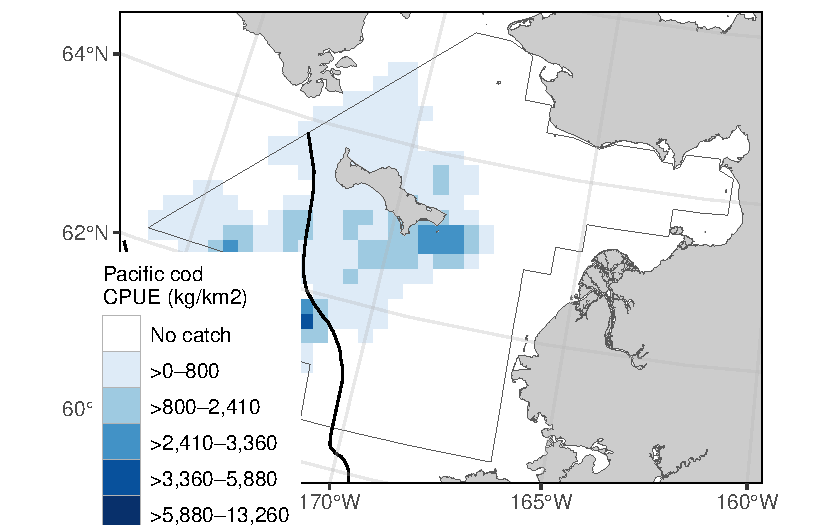
\includegraphics{content/foss-api-r_files/figure-pdf/test-7-fig-1.pdf}

}

\caption{Ex. 7: Visualize CPUE data in distribution map.}

\end{figure}

\hypertarget{access-api-data-using-python}{%
\chapter{Access API data using
Python}\label{access-api-data-using-python}}

\hypertarget{afscgap-library-installation}{%
\subsection{\{afscgap\} Library
Installation}\label{afscgap-library-installation}}

\begin{quote}
author: Sam Pottinger (sam.pottinger@berkeley.edu; GitHub::sampottinger)
date: May 13, 2023
\end{quote}

The third-party \texttt{afscgap} Python package interfaces with FOSS to
access AFSC GAP data. It can be installed via pip:

\begin{Shaded}
\begin{Highlighting}[]
\CommentTok{\#The reticulate package provides a comprehensive set of tools for interoperability between Python and R. }
\FunctionTok{library}\NormalTok{(reticulate)}
\end{Highlighting}
\end{Shaded}

\begin{Shaded}
\begin{Highlighting}[]
\NormalTok{pip install afscgap}
\NormalTok{pip install git}\SpecialCharTok{+}\NormalTok{https}\SpecialCharTok{:}\ErrorTok{//}\NormalTok{github.com}\SpecialCharTok{/}\NormalTok{SchmidtDSE}\SpecialCharTok{/}\NormalTok{afscgap.git}\SpecialCharTok{@}\NormalTok{main}
\end{Highlighting}
\end{Shaded}

For more information on installation and deployment, see the
\href{https://pyafscgap.org}{library documentation}.

\hypertarget{basic-query}{%
\subsection{Basic query}\label{basic-query}}

This first example queries for Pacific glass shrimp (\emph{Pasiphaea
pacifica}) in the Gulf of Alaska in 2021. The library will automatically
generate HTTP queries, converting from Python types to
\href{https://www.oracle.com/database/technologies/appdev/rest.html}{ORDS}
query syntax.

\begin{Shaded}
\begin{Highlighting}[]
\NormalTok{import afscgap}

\NormalTok{query }\OtherTok{=} \FunctionTok{afscgap.Query}\NormalTok{()}
\FunctionTok{query.filter\_year}\NormalTok{(}\AttributeTok{eq=}\DecValTok{2021}\NormalTok{)}
\FunctionTok{query.filter\_srvy}\NormalTok{(}\AttributeTok{eq=}\StringTok{\textquotesingle{}GOA\textquotesingle{}}\NormalTok{)}
\FunctionTok{query.filter\_scientific\_name}\NormalTok{(}\AttributeTok{eq=}\StringTok{\textquotesingle{}Pasiphaea pacifica\textquotesingle{}}\NormalTok{)}

\NormalTok{results }\OtherTok{=} \FunctionTok{query.execute}\NormalTok{()}
\end{Highlighting}
\end{Shaded}

The \texttt{results} variable in this example is an iterator that will
automatically perform pagination behind the scenes.

\hypertarget{iterating-with-a-for-loop}{%
\subsection{Iterating with a for loop}\label{iterating-with-a-for-loop}}

The easiest way to interact with results is a simple for loop. This next
example determines the frequency of different catch per unit effort
where Pacific glass shrimp were reported:

\begin{Shaded}
\begin{Highlighting}[]
\NormalTok{import afscgap}

\CommentTok{\# Mapping from CPUE to count}
\NormalTok{count\_by\_cpue }\OtherTok{=}\NormalTok{ \{\}}

\CommentTok{\# Build query}
\NormalTok{query }\OtherTok{=} \FunctionTok{afscgap.Query}\NormalTok{()}
\FunctionTok{query.filter\_year}\NormalTok{(}\AttributeTok{eq=}\DecValTok{2021}\NormalTok{)}
\FunctionTok{query.filter\_srvy}\NormalTok{(}\AttributeTok{eq=}\StringTok{\textquotesingle{}GOA\textquotesingle{}}\NormalTok{)}
\FunctionTok{query.filter\_scientific\_name}\NormalTok{(}\AttributeTok{eq=}\StringTok{\textquotesingle{}Pasiphaea pacifica\textquotesingle{}}\NormalTok{)}
\NormalTok{results }\OtherTok{=} \FunctionTok{query.execute}\NormalTok{()}

\CommentTok{\# Iterate through results and count}
\ControlFlowTok{for}\NormalTok{ record }\ControlFlowTok{in}\NormalTok{ results}\SpecialCharTok{:}
\NormalTok{  cpue }\OtherTok{=} \FunctionTok{record.get\_cpue\_weight}\NormalTok{(}\AttributeTok{units=}\StringTok{\textquotesingle{}kg/ha\textquotesingle{}}\NormalTok{)}
\NormalTok{  cpue\_rounded }\OtherTok{=} \FunctionTok{round}\NormalTok{(cpue)}
\NormalTok{  count }\OtherTok{=} \FunctionTok{count\_by\_cpue.get}\NormalTok{(cpue\_rounded, }\DecValTok{0}\NormalTok{) }\SpecialCharTok{+} \DecValTok{1}
\NormalTok{  count\_by\_cpue[cpue\_rounded] }\OtherTok{=}\NormalTok{ count}

\CommentTok{\# Print the result}
\FunctionTok{print}\NormalTok{(count\_by\_cpue)}
\end{Highlighting}
\end{Shaded}

Note that, in this example, only records with Pacific glass shrimp are
included (``presence-only'' data). See zero catch inference below. In
other words, it reports on CPUE only for hauls in which Pacific glass
shrimp were recorded, excluding some hauls like those in which Pacific
glass shrimp were not found at all.

\hypertarget{iterating-with-functional-programming}{%
\subsection{Iterating with functional
programming}\label{iterating-with-functional-programming}}

A for loop is not the only option for iterating through results. List
comprehensions and other functional programming methods can be used as
well.

\begin{Shaded}
\begin{Highlighting}[]
\NormalTok{import statistics}

\NormalTok{import afscgap}

\CommentTok{\# Build query}
\NormalTok{query }\OtherTok{=} \FunctionTok{afscgap.Query}\NormalTok{()}
\FunctionTok{query.filter\_year}\NormalTok{(}\AttributeTok{eq=}\DecValTok{2021}\NormalTok{)}
\FunctionTok{query.filter\_srvy}\NormalTok{(}\AttributeTok{eq=}\StringTok{\textquotesingle{}GOA\textquotesingle{}}\NormalTok{)}
\FunctionTok{query.filter\_scientific\_name}\NormalTok{(}\AttributeTok{eq=}\StringTok{\textquotesingle{}Pasiphaea pacifica\textquotesingle{}}\NormalTok{)}
\NormalTok{results }\OtherTok{=} \FunctionTok{query.execute}\NormalTok{()}

\CommentTok{\# Get temperatures in Celsius}
\NormalTok{temperatures }\OtherTok{=}\NormalTok{ [}\FunctionTok{record.get\_bottom\_temperature}\NormalTok{(}\AttributeTok{units=}\StringTok{\textquotesingle{}c\textquotesingle{}}\NormalTok{) }\ControlFlowTok{for}\NormalTok{ record }\ControlFlowTok{in}\NormalTok{ results]}

\CommentTok{\# Take the median}
\FunctionTok{print}\NormalTok{(}\FunctionTok{statistics.median}\NormalTok{(temperatures))}
\end{Highlighting}
\end{Shaded}

This example reports the median temperature in Celcius for when Pacific
glass shrimp was reported.

\hypertarget{load-into-pandas}{%
\subsection{Load into Pandas}\label{load-into-pandas}}

The results from the \texttt{afscgap} package are serializable and can
be loaded into other tools like
\href{https://pandas.pydata.org/}{Pandas}. This example loads Pacific
glass shrimp from 2021 Gulf of Alaska into a data frame.

\begin{Shaded}
\begin{Highlighting}[]
\NormalTok{import pandas}

\NormalTok{import afscgap}

\NormalTok{query }\OtherTok{=} \FunctionTok{afscgap.Query}\NormalTok{()}
\FunctionTok{query.filter\_year}\NormalTok{(}\AttributeTok{eq=}\DecValTok{2021}\NormalTok{)}
\FunctionTok{query.filter\_srvy}\NormalTok{(}\AttributeTok{eq=}\StringTok{\textquotesingle{}GOA\textquotesingle{}}\NormalTok{)}
\FunctionTok{query.filter\_scientific\_name}\NormalTok{(}\AttributeTok{eq=}\StringTok{\textquotesingle{}Pasiphaea pacifica\textquotesingle{}}\NormalTok{)}
\NormalTok{results }\OtherTok{=} \FunctionTok{query.execute}\NormalTok{()}

\FunctionTok{pandas.DataFrame}\NormalTok{(}\FunctionTok{results.to\_dicts}\NormalTok{())}
\end{Highlighting}
\end{Shaded}

Specifically, \texttt{to\_dicts} provides an iterator over a dictionary
form of the data that can be read into tools like Pandas.

\hypertarget{advanced-filtering}{%
\subsection{Advanced filtering}\label{advanced-filtering}}

Queries so far have focused on filters requiring equality but range
queries can be built as well.

\begin{Shaded}
\begin{Highlighting}[]
\NormalTok{import afscgap}

\CommentTok{\# Build query}
\NormalTok{query }\OtherTok{=} \FunctionTok{afscgap.Query}\NormalTok{()}
\FunctionTok{query.filter\_year}\NormalTok{(}\AttributeTok{min\_val=}\DecValTok{2015}\NormalTok{, }\AttributeTok{max\_val=}\DecValTok{2019}\NormalTok{)   }\CommentTok{\# Note min/max\_val}
\FunctionTok{query.filter\_srvy}\NormalTok{(}\AttributeTok{eq=}\StringTok{\textquotesingle{}GOA\textquotesingle{}}\NormalTok{)}
\FunctionTok{query.filter\_scientific\_name}\NormalTok{(}\AttributeTok{eq=}\StringTok{\textquotesingle{}Pasiphaea pacifica\textquotesingle{}}\NormalTok{)}
\NormalTok{results }\OtherTok{=} \FunctionTok{query.execute}\NormalTok{()}

\CommentTok{\# Sum weight}
\NormalTok{weights }\OtherTok{=} \FunctionTok{map}\NormalTok{(lambda x}\SpecialCharTok{:} \FunctionTok{x.get\_weight}\NormalTok{(}\AttributeTok{units=}\StringTok{\textquotesingle{}kg\textquotesingle{}}\NormalTok{), results)}
\NormalTok{total\_weight }\OtherTok{=} \FunctionTok{sum}\NormalTok{(weights)}
\FunctionTok{print}\NormalTok{(total\_weight)}
\end{Highlighting}
\end{Shaded}

This example queries for Pacific glass shrimp data between 2015 and
2019, summing the total weight caught. Note that most users will likely
take advantage of built-in Python to
\href{https://www.oracle.com/database/technologies/appdev/rest.html}{ORDS}
query generation which dictates how the library communicates with the
API service. However, users can provide raw ORDS queries as well using
\href{https://pyafscgap.org/devdocs/afscgap.html\#manual-filtering}{manual
filtering}.

\hypertarget{zero-catch-inference}{%
\subsection{Zero-catch inference}\label{zero-catch-inference}}

Until this point, these examples use presence-only data. However, the
\texttt{afscgap} package can infer negative or ``zero catch'' records as
well.

\begin{Shaded}
\begin{Highlighting}[]
\NormalTok{import afscgap}

\CommentTok{\# Mapping from CPUE to count}
\NormalTok{count\_by\_cpue }\OtherTok{=}\NormalTok{ \{\}}

\CommentTok{\# Build query}
\NormalTok{query }\OtherTok{=} \FunctionTok{afscgap.Query}\NormalTok{()}
\FunctionTok{query.filter\_year}\NormalTok{(}\AttributeTok{eq=}\DecValTok{2021}\NormalTok{)}
\FunctionTok{query.filter\_srvy}\NormalTok{(}\AttributeTok{eq=}\StringTok{\textquotesingle{}GOA\textquotesingle{}}\NormalTok{)}
\FunctionTok{query.filter\_scientific\_name}\NormalTok{(}\AttributeTok{eq=}\StringTok{\textquotesingle{}Pasiphaea pacifica\textquotesingle{}}\NormalTok{)}
\FunctionTok{query.set\_presence\_only}\NormalTok{(False)  }\CommentTok{\# Added to earlier example}
\NormalTok{results }\OtherTok{=} \FunctionTok{query.execute}\NormalTok{()}

\CommentTok{\# Iterate through results and count}
\ControlFlowTok{for}\NormalTok{ record }\ControlFlowTok{in}\NormalTok{ results}\SpecialCharTok{:}
\NormalTok{  cpue }\OtherTok{=} \FunctionTok{record.get\_cpue\_weight}\NormalTok{(}\AttributeTok{units=}\StringTok{\textquotesingle{}kg/ha\textquotesingle{}}\NormalTok{)}
\NormalTok{  cpue\_rounded }\OtherTok{=} \FunctionTok{round}\NormalTok{(cpue)}
\NormalTok{  count }\OtherTok{=} \FunctionTok{count\_by\_cpue.get}\NormalTok{(cpue\_rounded, }\DecValTok{0}\NormalTok{) }\SpecialCharTok{+} \DecValTok{1}
\NormalTok{  count\_by\_cpue[cpue\_rounded] }\OtherTok{=}\NormalTok{ count}

\CommentTok{\# Print the result}
\FunctionTok{print}\NormalTok{(count\_by\_cpue)}
\end{Highlighting}
\end{Shaded}

This example revisits the earlier snippet for CPUE counts but
\texttt{set\_presence\_only(False)} directs the library to look at
additional data on hauls, determining which hauls did not have Pacific
glass shrimp. This lets the library return records for hauls in which
Pacific glass shrimp were not found. This can be seen in differences in
counts reported:

\begin{longtable}[]{@{}
  >{\raggedright\arraybackslash}p{(\columnwidth - 4\tabcolsep) * \real{0.1609}}
  >{\raggedright\arraybackslash}p{(\columnwidth - 4\tabcolsep) * \real{0.4138}}
  >{\raggedright\arraybackslash}p{(\columnwidth - 4\tabcolsep) * \real{0.4253}}@{}}
\toprule\noalign{}
\begin{minipage}[b]{\linewidth}\raggedright
Rounded CPUE
\end{minipage} & \begin{minipage}[b]{\linewidth}\raggedright
Count with set\_presence\_only(True)
\end{minipage} & \begin{minipage}[b]{\linewidth}\raggedright
Count with set\_presence\_only(False)
\end{minipage} \\
\midrule\noalign{}
\endhead
\bottomrule\noalign{}
\endlastfoot
0 kg/ha & 44 & 521 \\
1 kg/ha & 7 & 7 \\
2 kg/ha & 1 & 1 \\
\end{longtable}

Put simply, while the earlier example showed CPUE counts for hauls in
which Pacific glass shrimp were seen, this revised example reports for
all hauls in the Gulf of Alaska in 2021.

\hypertarget{more-information}{%
\subsection{More information}\label{more-information}}

Please see the \href{https://pyafscgap.org/devdocs/afscgap.html}{API
documentation} for the Python library for additional details.

\hypertarget{access-data-using-r-afsc-only}{%
\chapter{Access data using R (AFSC
only)}\label{access-data-using-r-afsc-only}}

If the user has access to the AFSC \texttt{Oracle} database, the user
can use \texttt{SQL\ developer} to view and pull the FOSS public data
directly from the \texttt{RACEBASE\_FOSS} \texttt{Oracle} schema.

\hypertarget{connect-to-oracle-from-r-1}{%
\subsection{Connect to Oracle from R}\label{connect-to-oracle-from-r-1}}

Many users will want to access the data from \texttt{Oracle} using
\texttt{R}. The user will need to install the \texttt{RODBC} \texttt{R}
package and ask OFIS (IT) connect \texttt{R} to \texttt{Oracle}. Then,
use the following code in \texttt{R} to establish a connection from
\texttt{R} to \texttt{Oracle}:

Here, the user can write in their username and password directly into
the \texttt{RODBC} connect function. Never save usernames or passwords
in scripts that may be intentionally or unintentionally shared with
others. If no username and password is entered in the function, pop-ups
will appear on the screen asking for the username and password.

\begin{Shaded}
\begin{Highlighting}[]
 \CommentTok{\#\textquotesingle{} Define RODBC connection to ORACLE}
 \CommentTok{\#\textquotesingle{}}
 \CommentTok{\#\textquotesingle{} @param schema default = \textquotesingle{}AFSC\textquotesingle{}. }
 \CommentTok{\#\textquotesingle{}}
 \CommentTok{\#\textquotesingle{} @return oracle channel connection}
 \CommentTok{\#\textquotesingle{} @export}
 \CommentTok{\#\textquotesingle{}}
 \CommentTok{\#\textquotesingle{} @examples}
 \CommentTok{\#\textquotesingle{} \# Not run}
 \CommentTok{\#\textquotesingle{} \# channel \textless{}{-} oracle\_connect()}
\NormalTok{oracle\_connect }\OtherTok{\textless{}{-}} \ControlFlowTok{function}\NormalTok{(}
    \AttributeTok{schema=}\StringTok{\textquotesingle{}AFSC\textquotesingle{}}\NormalTok{, }
    \AttributeTok{username =} \ConstantTok{NULL}\NormalTok{, }
    \AttributeTok{passowrd =} \ConstantTok{NULL}\NormalTok{)\{(}\AttributeTok{echo=}\ConstantTok{FALSE}\NormalTok{)}
  
  \FunctionTok{library}\NormalTok{(}\StringTok{"RODBC"}\NormalTok{)}
  \FunctionTok{library}\NormalTok{(}\StringTok{"getPass"}\NormalTok{)}
  \ControlFlowTok{if}\NormalTok{ (}\FunctionTok{is.null}\NormalTok{(username)) \{}
\NormalTok{    username }\OtherTok{\textless{}{-}} \FunctionTok{getPass}\NormalTok{(}\AttributeTok{msg =} \StringTok{"Enter your ORACLE Username: "}\NormalTok{)}
\NormalTok{  \}}
  \ControlFlowTok{if}\NormalTok{ (}\FunctionTok{is.null}\NormalTok{(password)) \{}
\NormalTok{    password }\OtherTok{\textless{}{-}} \FunctionTok{getPass}\NormalTok{(}\AttributeTok{msg =} \StringTok{"Enter your ORACLE Password: "}\NormalTok{)}
\NormalTok{  \}}
\NormalTok{  channel  }\OtherTok{\textless{}{-}}\NormalTok{ RODBC}\SpecialCharTok{::}\FunctionTok{odbcConnect}\NormalTok{(}
    \FunctionTok{paste}\NormalTok{(schema),}
    \FunctionTok{paste}\NormalTok{(username),}
    \FunctionTok{paste}\NormalTok{(password), }
    \AttributeTok{believeNRows=}\ConstantTok{FALSE}\NormalTok{)}
  \FunctionTok{return}\NormalTok{(channel)}
\NormalTok{\}}

\NormalTok{channel }\OtherTok{\textless{}{-}} \FunctionTok{oracle\_connect}\NormalTok{()}
\end{Highlighting}
\end{Shaded}

\hypertarget{ex.-1-join-data}{%
\subsection{Ex. 1: Join data}\label{ex.-1-join-data}}

To join these tables in Oracle, you may use a variant of the following
code:

\hypertarget{ex.-2-subset-data}{%
\subsection{Ex. 2: Subset data}\label{ex.-2-subset-data}}

Once connected, pull and save (if needed) the tables into the \texttt{R}
environment.

To pull a small subset of the data (especially since files like
\texttt{RACEBASE\_FOSS.FOSS\_CPUE\_ZEROFILLED} are so big), use a
variation of the following code. Here, we are pulling EBS Pacific cod
from 2010 - 2021:

\begin{Shaded}
\begin{Highlighting}[]
\CommentTok{\# Pull data}
\NormalTok{a }\OtherTok{\textless{}{-}}\NormalTok{ RODBC}\SpecialCharTok{::}\FunctionTok{sqlQuery}\NormalTok{(}
\AttributeTok{channel =}\NormalTok{ channel, }
\AttributeTok{query =} 
\StringTok{"SELECT * FROM GAP\_PRODUCTS.FOSS\_CATCH cc}
\StringTok{JOIN GAP\_PRODUCTS.FOSS\_HAUL hh}
\StringTok{ON cc.HAULJOIN = hh.HAULJOIN}
\StringTok{WHERE SRVY = \textquotesingle{}EBS\textquotesingle{} }
\StringTok{AND COMMON\_NAME = \textquotesingle{}Pacific cod\textquotesingle{} }
\StringTok{AND YEAR \textgreater{}= 2010 }
\StringTok{AND YEAR \textless{} 2021"}\NormalTok{)}
\CommentTok{\# Save table to local directory}
\FunctionTok{write.csv}\NormalTok{(}\AttributeTok{x =}\NormalTok{ a, }\AttributeTok{file =} \StringTok{"RACEBASE\_FOSS{-}FOSS\_CPUE\_ZEROFILLED{-}ebs\_pcod\_2010{-}2020.csv"}\NormalTok{)}
\end{Highlighting}
\end{Shaded}

\part{Notes}

Thank you for using our data guide!

\hypertarget{production-run-notes}{%
\chapter{Production Run Notes}\label{production-run-notes}}

\hypertarget{r-version-metadata}{%
\chapter{R Version Metadata}\label{r-version-metadata}}

\begin{verbatim}
R version 4.3.0 (2023-04-21 ucrt)
Platform: x86_64-w64-mingw32/x64 (64-bit)
Running under: Windows 10 x64 (build 19045)

Matrix products: default


locale:
[1] LC_COLLATE=English_United States.utf8 
[2] LC_CTYPE=English_United States.utf8   
[3] LC_MONETARY=English_United States.utf8
[4] LC_NUMERIC=C                          
[5] LC_TIME=English_United States.utf8    

time zone: America/Los_Angeles
tzcode source: internal

attached base packages:
[1] stats     graphics  grDevices utils     datasets  methods   base     

loaded via a namespace (and not attached):
 [1] compiler_4.3.0    fastmap_1.1.1     cli_3.6.1         tools_4.3.0      
 [5] htmltools_0.5.5   rstudioapi_0.15.0 yaml_2.3.7        rmarkdown_2.23   
 [9] knitr_1.43        jsonlite_1.8.7    xfun_0.39         digest_0.6.33    
[13] rlang_1.1.1       evaluate_0.21    
\end{verbatim}

\hypertarget{noaa-readme}{%
\subsection{NOAA README}\label{noaa-readme}}

This repository is a scientific product and is not official
communication of the National Oceanic and Atmospheric Administration, or
the United States Department of Commerce. All NOAA GitHub project code
is provided on an `as is' basis and the user assumes responsibility for
its use. Any claims against the Department of Commerce or Department of
Commerce bureaus stemming from the use of this GitHub project will be
governed by all applicable Federal law. Any reference to specific
commercial products, processes, or services by service mark, trademark,
manufacturer, or otherwise, does not constitute or imply their
endorsement, recommendation or favoring by the Department of Commerce.
The Department of Commerce seal and logo, or the seal and logo of a DOC
bureau, shall not be used in any manner to imply endorsement of any
commercial product or activity by DOC or the United States Government.

\hypertarget{noaa-license}{%
\subsection{NOAA License}\label{noaa-license}}

Software code created by U.S. Government employees is not subject to
copyright in the United States (17 U.S.C. §105). The United
States/Department of Commerce reserve all rights to seek and obtain
copyright protection in countries other than the United States for
Software authored in its entirety by the Department of Commerce. To this
end, the Department of Commerce hereby grants to Recipient a
royalty-free, nonexclusive license to use, copy, and create derivative
works of the Software outside of the United States.

\hypertarget{acknowledgments}{%
\chapter{Acknowledgments}\label{acknowledgments}}

\hypertarget{community-acknowledgments}{%
\chapter{Community Acknowledgments}\label{community-acknowledgments}}

We would like to thank the many communities of Alaska and their members
who have helped contribute to this body of work. The knowledge,
experiences, and insights have been instrumental in expanding the scope
of our science and knowledge to encompass the many issues that face this
important ecosystem. We appreciate feedback from those residing in the
region that are willing to share their insights and participation in an
open dialog about how we can improve our collective knowledge of the
ecosystem and the region.

\hypertarget{technical-acknowledgments}{%
\chapter{Technical Acknowledgments}\label{technical-acknowledgments}}

This quarto book is based off the
\href{https://github.com/nmfs-opensci/NOAA-quarto-book}{NOAA-quarto-book}
GitHub repo designed by Eli Holmes.

This repo and GitHub Action was based on the tutorial by Openscapes
\href{https://github.com/Openscapes/quarto-website-tutorial}{quarto-website-tutorial}
by Julia Lowndes and Stefanie Butland.

\hypertarget{partners}{%
\section{Partners}\label{partners}}

Scientists from the Alaska Fisheries Science Center conduct these bottom
trawl surveys with participation from the Alaska Department of Fish \&
Game (ADF\&G), the International Pacific Halibut Commission (IPHC), and
universities. This research is conducted on chartered fishing vessels.

\hypertarget{references}{%
\chapter{References}\label{references}}

\hypertarget{refs}{}
\begin{CSLReferences}{1}{0}
\leavevmode\vadjust pre{\hypertarget{ref-GAPakfin}{}}%
Alaska Fisheries Information Network (AKFIN). (2023). \emph{AFSC
goundfish assessment program design-based production data}. {NOAA
Fisheries Alaska Fisheries Science Center, Goundfish Assessment
Program};
https://www.psmfc.org/program/alaska-fisheries-information-network-akfin;
{U.S. Dep. Commer.}

\leavevmode\vadjust pre{\hypertarget{ref-RN979}{}}%
Hoff, G. R. (2016). \emph{Results of the 2016 eastern {Bering Sea} upper
continental slope survey of groundfishes and invertebrate resources}
(NOAA Tech. Memo. NOAA-AFSC-339). {U.S. Dep. Commer.}
\url{https://doi.org/10.7289/V5/TM-AFSC-339}

\leavevmode\vadjust pre{\hypertarget{ref-2022NEBS2023}{}}%
Markowitz, E. H., Dawson, E. J., Anderson, A. B., Rohan, S. K.,
Charriere, N. E., Prohaska, B. K., and Stevenson, D. E. (2023).
\emph{Results of the 2022 eastern and northern {Bering Sea} continental
shelf bottom trawl survey of groundfish and invertebrate fauna} (NOAA
Tech. Memo. NMFS-AFSC-469; p. 213). {U.S. Dep. Commer.}

\leavevmode\vadjust pre{\hypertarget{ref-FOSSAFSCData}{}}%
NOAA Fisheries Alaska Fisheries Science Center. (2023). \emph{Fisheries
one stop shop public data: RACE division bottom trawl survey data
query}. https://www.fisheries.noaa.gov/foss; {U.S. Dep. Commer.}

\leavevmode\vadjust pre{\hypertarget{ref-GAPProducts}{}}%
NOAA Fisheries Alaska Fisheries Science Center, Goundfish Assessment
Program. (2023). \emph{AFSC goundfish assessment program design-based
production data}.
https://www.fisheries.noaa.gov/alaska/science-data/groundfish-assessment-program-bottom-trawl-surveys;
{U.S. Dep. Commer.}

\leavevmode\vadjust pre{\hypertarget{ref-GOA2018}{}}%
Von Szalay, P. G., and Raring, N. W. (2018). \emph{Data report: 2017
{Gulf of Alaska} bottom trawl survey} (NOAA Tech. Memo. NMFS-AFSC-374).
{U.S. Dep. Commer.} \url{https://doi.org/10.7289/V5/TM-AFSC-374}

\leavevmode\vadjust pre{\hypertarget{ref-AI2018}{}}%
Von Szalay, P. G., and Raring, N. W. (2020). \emph{Data report: 2018
{Aleutian Islands} bottom trawl survey} (NOAA Tech. Memo.
NMFS-AFSC-409). {U.S. Dep. Commer.}
\url{https://doi.org/10.25923/qe5v-fz70}

\end{CSLReferences}

\hypertarget{contact-us}{%
\chapter{Contact us}\label{contact-us}}

\textbf{General questions and more specific data requests} can be sent
to
\href{mailto:afsc.gap.metadata@noaa.gov}{\nolinkurl{afsc.gap.metadata@noaa.gov}}
or submitted as an
\href{https://github.com/afsc-gap-products/data-requests}{issue on our
GitHub Organization}. The version of this data used for stock
assessments can be found through the Alaska Fisheries Information
Network (AKFIN). For questions about the eastern Bering Sea surveys,
contact Duane Stevenson
(\href{mailto:Duane.Stevenson@noaa.gov}{\nolinkurl{Duane.Stevenson@noaa.gov}}).
For questions about the Gulf of Alaska or Aleutian Islands surveys,
contact Ned Laman
(\href{mailto:Ned.Laman@noaa.gov}{\nolinkurl{Ned.Laman@noaa.gov}}). For
questions specifically about crab data in any region, contact Mike
Litzow
(\href{mailto:Mike.Litzow@noaa.gov}{\nolinkurl{Mike.Litzow@noaa.gov}}),
the Shellfish Assessment Program lead.

For questions, comments, and concerns specifically about the
\href{https://www.fisheries.noaa.gov/foss}{Fisheries One Stop Shop
(FOSS)} platform, please contact us using the Comments page on the
\href{https://www.fisheries.noaa.gov/foss}{FOSS} webpage.

Alaska Fisheries Science Center (AFSC)\\
National Oceanic and Atmospheric Administration (NOAA)\\
Resource Assessment and Conservation Engineering Division (RACE)\\
Groundfish Assessment Program (GAP)\\
7600 Sand Point Way, N.E. bldg. 4\\
Seattle, WA 98115 USA

\hypertarget{suggestions-and-comments}{%
\section{Suggestions and comments}\label{suggestions-and-comments}}

If the data or metadata can be improved, please create a pull request,
\href{https://github.com/afsc-gap-products/data-requests/issues}{submit
an issue to the GitHub organization} or
\href{https://github.com/afsc-gap-products/gap_products/issues}{submit
an issue to the code's repository}.


\backmatter

\end{document}
